% Options for packages loaded elsewhere
\PassOptionsToPackage{unicode}{hyperref}
\PassOptionsToPackage{hyphens}{url}
%
\documentclass[
]{scrbook}
\usepackage{lmodern}
\usepackage{amssymb,amsmath}
\usepackage{ifxetex,ifluatex}
\ifnum 0\ifxetex 1\fi\ifluatex 1\fi=0 % if pdftex
  \usepackage[T1]{fontenc}
  \usepackage[utf8]{inputenc}
  \usepackage{textcomp} % provide euro and other symbols
\else % if luatex or xetex
  \usepackage{unicode-math}
  \defaultfontfeatures{Scale=MatchLowercase}
  \defaultfontfeatures[\rmfamily]{Ligatures=TeX,Scale=1}
\fi
% Use upquote if available, for straight quotes in verbatim environments
\IfFileExists{upquote.sty}{\usepackage{upquote}}{}
\IfFileExists{microtype.sty}{% use microtype if available
  \usepackage[]{microtype}
  \UseMicrotypeSet[protrusion]{basicmath} % disable protrusion for tt fonts
}{}
\makeatletter
\@ifundefined{KOMAClassName}{% if non-KOMA class
  \IfFileExists{parskip.sty}{%
    \usepackage{parskip}
  }{% else
    \setlength{\parindent}{0pt}
    \setlength{\parskip}{6pt plus 2pt minus 1pt}}
}{% if KOMA class
  \KOMAoptions{parskip=half}}
\makeatother
\usepackage{xcolor}
\IfFileExists{xurl.sty}{\usepackage{xurl}}{} % add URL line breaks if available
\IfFileExists{bookmark.sty}{\usepackage{bookmark}}{\usepackage{hyperref}}
\hypersetup{
  pdftitle={Simulation Modeling and Arena},
  pdfauthor={Manuel D. Rossetti},
  hidelinks,
  pdfcreator={LaTeX via pandoc}}
\urlstyle{same} % disable monospaced font for URLs
\usepackage{color}
\usepackage{fancyvrb}
\newcommand{\VerbBar}{|}
\newcommand{\VERB}{\Verb[commandchars=\\\{\}]}
\DefineVerbatimEnvironment{Highlighting}{Verbatim}{commandchars=\\\{\}}
% Add ',fontsize=\small' for more characters per line
\usepackage{framed}
\definecolor{shadecolor}{RGB}{248,248,248}
\newenvironment{Shaded}{\begin{snugshade}}{\end{snugshade}}
\newcommand{\AlertTok}[1]{\textcolor[rgb]{0.94,0.16,0.16}{#1}}
\newcommand{\AnnotationTok}[1]{\textcolor[rgb]{0.56,0.35,0.01}{\textbf{\textit{#1}}}}
\newcommand{\AttributeTok}[1]{\textcolor[rgb]{0.77,0.63,0.00}{#1}}
\newcommand{\BaseNTok}[1]{\textcolor[rgb]{0.00,0.00,0.81}{#1}}
\newcommand{\BuiltInTok}[1]{#1}
\newcommand{\CharTok}[1]{\textcolor[rgb]{0.31,0.60,0.02}{#1}}
\newcommand{\CommentTok}[1]{\textcolor[rgb]{0.56,0.35,0.01}{\textit{#1}}}
\newcommand{\CommentVarTok}[1]{\textcolor[rgb]{0.56,0.35,0.01}{\textbf{\textit{#1}}}}
\newcommand{\ConstantTok}[1]{\textcolor[rgb]{0.00,0.00,0.00}{#1}}
\newcommand{\ControlFlowTok}[1]{\textcolor[rgb]{0.13,0.29,0.53}{\textbf{#1}}}
\newcommand{\DataTypeTok}[1]{\textcolor[rgb]{0.13,0.29,0.53}{#1}}
\newcommand{\DecValTok}[1]{\textcolor[rgb]{0.00,0.00,0.81}{#1}}
\newcommand{\DocumentationTok}[1]{\textcolor[rgb]{0.56,0.35,0.01}{\textbf{\textit{#1}}}}
\newcommand{\ErrorTok}[1]{\textcolor[rgb]{0.64,0.00,0.00}{\textbf{#1}}}
\newcommand{\ExtensionTok}[1]{#1}
\newcommand{\FloatTok}[1]{\textcolor[rgb]{0.00,0.00,0.81}{#1}}
\newcommand{\FunctionTok}[1]{\textcolor[rgb]{0.00,0.00,0.00}{#1}}
\newcommand{\ImportTok}[1]{#1}
\newcommand{\InformationTok}[1]{\textcolor[rgb]{0.56,0.35,0.01}{\textbf{\textit{#1}}}}
\newcommand{\KeywordTok}[1]{\textcolor[rgb]{0.13,0.29,0.53}{\textbf{#1}}}
\newcommand{\NormalTok}[1]{#1}
\newcommand{\OperatorTok}[1]{\textcolor[rgb]{0.81,0.36,0.00}{\textbf{#1}}}
\newcommand{\OtherTok}[1]{\textcolor[rgb]{0.56,0.35,0.01}{#1}}
\newcommand{\PreprocessorTok}[1]{\textcolor[rgb]{0.56,0.35,0.01}{\textit{#1}}}
\newcommand{\RegionMarkerTok}[1]{#1}
\newcommand{\SpecialCharTok}[1]{\textcolor[rgb]{0.00,0.00,0.00}{#1}}
\newcommand{\SpecialStringTok}[1]{\textcolor[rgb]{0.31,0.60,0.02}{#1}}
\newcommand{\StringTok}[1]{\textcolor[rgb]{0.31,0.60,0.02}{#1}}
\newcommand{\VariableTok}[1]{\textcolor[rgb]{0.00,0.00,0.00}{#1}}
\newcommand{\VerbatimStringTok}[1]{\textcolor[rgb]{0.31,0.60,0.02}{#1}}
\newcommand{\WarningTok}[1]{\textcolor[rgb]{0.56,0.35,0.01}{\textbf{\textit{#1}}}}
\usepackage{longtable,booktabs}
% Correct order of tables after \paragraph or \subparagraph
\usepackage{etoolbox}
\makeatletter
\patchcmd\longtable{\par}{\if@noskipsec\mbox{}\fi\par}{}{}
\makeatother
% Allow footnotes in longtable head/foot
\IfFileExists{footnotehyper.sty}{\usepackage{footnotehyper}}{\usepackage{footnote}}
\makesavenoteenv{longtable}
\usepackage{graphicx}
\makeatletter
\def\maxwidth{\ifdim\Gin@nat@width>\linewidth\linewidth\else\Gin@nat@width\fi}
\def\maxheight{\ifdim\Gin@nat@height>\textheight\textheight\else\Gin@nat@height\fi}
\makeatother
% Scale images if necessary, so that they will not overflow the page
% margins by default, and it is still possible to overwrite the defaults
% using explicit options in \includegraphics[width, height, ...]{}
\setkeys{Gin}{width=\maxwidth,height=\maxheight,keepaspectratio}
% Set default figure placement to htbp
\makeatletter
\def\fps@figure{htbp}
\makeatother
\setlength{\emergencystretch}{3em} % prevent overfull lines
\providecommand{\tightlist}{%
  \setlength{\itemsep}{0pt}\setlength{\parskip}{0pt}}
\setcounter{secnumdepth}{5}
\usepackage{booktabs}
\usepackage{longtable}
\usepackage[bf,singlelinecheck=off]{caption}
%\usepackage{subcaption}
\usepackage{placeins}
\usepackage{Alegreya}
\usepackage[scale=.7]{sourcecodepro}

\usepackage{framed,color}
\definecolor{shadecolor}{RGB}{248,248,248}

\renewcommand{\textfraction}{0.05}
\renewcommand{\topfraction}{0.8}
\renewcommand{\bottomfraction}{0.8}
\renewcommand{\floatpagefraction}{0.75}

% commended MDR 2-14-2021
%\renewenvironment{quote}{\begin{VF}}{\end{VF}}
\let\oldhref\href
\renewcommand{\href}[2]{#2\footnote{\url{#1}}}

\ifxetex
  \usepackage{letltxmacro}
  \setlength{\XeTeXLinkMargin}{1pt}
  \LetLtxMacro\SavedIncludeGraphics\includegraphics
  \def\includegraphics#1#{% #1 catches optional stuff (star/opt. arg.)
    \IncludeGraphicsAux{#1}%
  }%
  \newcommand*{\IncludeGraphicsAux}[2]{%
    \XeTeXLinkBox{%
      \SavedIncludeGraphics#1{#2}%
    }%
  }%
\fi

\makeatletter
\newenvironment{kframe}{%
\medskip{}
\setlength{\fboxsep}{.8em}
 \def\at@end@of@kframe{}%
 \ifinner\ifhmode%
  \def\at@end@of@kframe{\end{minipage}}%
  \begin{minipage}{\columnwidth}%
 \fi\fi%
 \def\FrameCommand##1{\hskip\@totalleftmargin \hskip-\fboxsep
 \colorbox{shadecolor}{##1}\hskip-\fboxsep
     % There is no \\@totalrightmargin, so:
     \hskip-\linewidth \hskip-\@totalleftmargin \hskip\columnwidth}%
 \MakeFramed {\advance\hsize-\width
   \@totalleftmargin\z@ \linewidth\hsize
   \@setminipage}}%
 {\par\unskip\endMakeFramed%
 \at@end@of@kframe}
\makeatother

\makeatletter
\@ifundefined{Shaded}{
}{\renewenvironment{Shaded}{\begin{kframe}}{\end{kframe}}}
\makeatother

\newenvironment{rmdblock}[1]
  {
  \begin{itemize}
  \renewcommand{\labelitemi}{
    \raisebox{-.7\height}[0pt][0pt]{
      {\setkeys{Gin}{width=3em,keepaspectratio}\includegraphics{images/#1}}
    }
  }
  \setlength{\fboxsep}{1em}
  \begin{kframe}
  \item
  }
  {
  \end{kframe}
  \end{itemize}
  }
\newenvironment{rmdnote}
  {\begin{rmdblock}{note}}
  {\end{rmdblock}}
\newenvironment{rmdcaution}
  {\begin{rmdblock}{caution}}
  {\end{rmdblock}}
\newenvironment{rmdimportant}
  {\begin{rmdblock}{important}}
  {\end{rmdblock}}
\newenvironment{rmdtip}
  {\begin{rmdblock}{tip}}
  {\end{rmdblock}}
\newenvironment{rmdwarning}
  {\begin{rmdblock}{warning}}
  {\end{rmdblock}}

\usepackage{makeidx}
\makeindex

\urlstyle{tt}

\usepackage{amsthm}
\makeatletter
\def\thm@space@setup{%
  \thm@preskip=8pt plus 2pt minus 4pt
  \thm@postskip=\thm@preskip
}

\makeatother

% added by MDR 2-14-2021
\newcommand{\dx}{\ensuremath{\,\mathrm{d}x}}
\newcommand{\DD}[1]{\ensuremath{\,\mathrm{d}#1}}
\newcommand{\RS}[2][n]{\ensuremath{#2_1, #2_2,\ldots, #2_{#1}}}
\newcommand{\RSX}{\RS{X}}
\newcommand{\RSY}{\RS{Y}}
\newcommand{\Xbar}{\ensuremath{\bar{X}}}
\newcommand{\Ybar}{\ensuremath{\bar{Y}}}
\newcommand{\Avg}[2][n]
{\ensuremath{\dfrac{1}{#1}\sum\limits_{i = 1}^{#1}{{#2_i}} }}
\newcommand{\Var}[2][n]
{\ensuremath{\dfrac{1}{{#1 - 1}}\sum\limits_{i = 1}^{#1} {{{\left( {{#2_i} - \bar{#2}} \right)}^2}}}}
\newcommand{\Prb}[1]{\ensuremath{\operatorname{P}\lbrace #1 \rbrace}}
\newcommand{\E}[1]{\ensuremath{\operatorname{E}\lbrack #1 \rbrack}}
\newcommand{\Esub}[2]{\ensuremath{\operatorname{E}_{#1}\lbrack #2 \rbrack}}
\newcommand{\V}[1]{\ensuremath{\operatorname{Var}\lbrack #1 \rbrack}}
\newcommand{\COR}[2]{\ensuremath{\operatorname{Corr}\lbrack #1, #2 \rbrack}}
\newcommand{\COV}[2]{\ensuremath{\operatorname{Cov}\lbrack #1, #2 \rbrack}}
% end added by MDR 2-14-2021

\frontmatter

\usepackage[ruled,vlined,linesnumbered]{algorithm2e}
\usepackage{subfig}
\usepackage{booktabs}
\usepackage{longtable}
\usepackage{array}
\usepackage{multirow}
\usepackage{wrapfig}
\usepackage{float}
\usepackage{colortbl}
\usepackage{pdflscape}
\usepackage{tabu}
\usepackage{threeparttable}
\usepackage{threeparttablex}
\usepackage[normalem]{ulem}
\usepackage{makecell}
\usepackage{xcolor}
\ifluatex
  \usepackage{selnolig}  % disable illegal ligatures
\fi
\usepackage[]{natbib}
\bibliographystyle{apalike}

\title{Simulation Modeling and Arena}
\author{Manuel D. Rossetti}
\date{2021-09-05}

\usepackage{amsthm}
\newtheorem{theorem}{Theorem}[chapter]
\newtheorem{lemma}{Lemma}[chapter]
\newtheorem{corollary}{Corollary}[chapter]
\newtheorem{proposition}{Proposition}[chapter]
\newtheorem{conjecture}{Conjecture}[chapter]
\theoremstyle{definition}
\newtheorem{definition}{Definition}[chapter]
\theoremstyle{definition}
\newtheorem{example}{Example}[chapter]
\theoremstyle{definition}
\newtheorem{exercise}{Exercise}[chapter]
\theoremstyle{remark}
\newtheorem*{remark}{Remark}
\newtheorem*{solution}{Solution}
\begin{document}
\maketitle

%\cleardoublepage\newpage\thispagestyle{empty}\null
%\cleardoublepage\newpage\thispagestyle{empty}\null
%\cleardoublepage\newpage
\thispagestyle{empty}
\begin{center}
%\includegraphics{images/dedication.pdf}
\end{center}

\setlength{\abovedisplayskip}{-5pt}
\setlength{\abovedisplayshortskip}{-5pt}

{
\setcounter{tocdepth}{2}
\tableofcontents
}
\hypertarget{preface}{%
\chapter*{Preface}\label{preface}}



\includegraphics{figures2/by-nc-nd.png}\\
This work is licensed under the \href{http://creativecommons.org/licenses/by-nc-nd/4.0/}{Creative Commons Attribution-NonCommercial-NoDerivatives 4.0 International License}.

Cover art image based on \href{https://pixabay.com/illustrations/time-clock-watches-wave-time-of-2132452/}{Time} by \href{https://pixabay.com/users/geralt-9301/?utm_source=link-attribution\&utm_medium=referral\&utm_campaign=image\&utm_content=2132452}{Gerd Altmann} from \href{https://pixabay.com/?utm_source=link-attribution\&utm_medium=referral\&utm_campaign=image\&utm_content=2132452}{Pixabay}

Welcome to the open text edition. Similarly to the previous two editions, the book is intended as an introductory textbook for a first course in discrete-event simulation modeling and analysis for upper-level undergraduate students as well as entering graduate students. While the text is focused towards engineering students (primarily industrial engineering) it could also be utilized by advanced business majors, computer science majors, and other disciplines where simulation is practiced. Practitioners interested in learning simulation and Arena could also use this book independently of a course.

\href{https://uark.libwizard.com/f/UA_OER_Adoption}{Adopt this book!} for your classes. We would appreciate it if you decide to adopt this book for use in courses that you let us know. Thanks!

When citing this book, please use the following format:

Rossetti, M.D.~(2021). Simulation Modeling and Arena, 3rd and Open Text Edition. Retrieved from \url{https://rossetti.github.io/RossettiArenaBook/} licensed under the \href{https://creativecommons.org/licenses/by-nc-nd/4.0/}{Creative Commons Attribution-NonCommercial-NoDerivatives 4.0 International License}.

\textbf{Release History}

You are reading the 3rd edition of \emph{Simulation Modeling and Arena} by Dr.~Manuel D. Rossetti. Because of its on-line nature, updated versions of the book will be released, as needed, to correct issues and possibly add new material that would not warrant a new edition. This section summarizes noteworthy updates.

\begin{itemize}
\tightlist
\item
  3rd Edition, Version 1.0, released June 14, 2021

  \begin{itemize}
  \tightlist
  \item
    first main release of text book
  \item
    files and supporting materials are related to Arena, version 16.0
  \end{itemize}
\end{itemize}

If you find typographical errors or other issues related to the text or supporting files, then please use the \href{https://github.com/rossetti/RossettiArenaBook}{repository's} issue tracking system to create a new issue. You should first check if the same or similar issue has already been submitted. The issue tracking system is for filing issues about the correctness of the text or files. It is \textbf{not} about general questions about simulation concepts, solutions to homework, how to do something in Arena, etc. Such issues will not be considered and will be deleted as needed.

\hypertarget{book-support-files}{%
\section*{Book Support Files}\label{book-support-files}}


By cloning the repository or downloading the zip archive, you can have a local copy of the entire book. Thus, if you do not have regular access to internet services, you can still read and utilize the materials. I encourage students within a class setting to clone the repository using a program such as Github desktop.

The example models and related files associated with the textbook are also copyrighted under the \emph{Creative Commons Attribution-NonCommercial-NoDerivatives 4.0 International License}. You may use the model files and other supporting data and spreadsheet files at your discretion. The files come as-is, with no warranty or other obligations implied. You can find the book support files at the following links.

\begin{itemize}
\tightlist
\item
  \href{https://uark.box.com/v/RossettiBookChapterFiles}{Chapter Files}
\item
  \href{https://uark.box.com/v/RossettiBookChapterSlides}{Chapter Slides}
\item
  Welch Plot Application

  \begin{itemize}
  \tightlist
  \item
    \href{https://uark.box.com/v/RossettiWelchPlotMacVersion}{Mac OS Version}
  \item
    \href{https://uark.box.com/v/RossettiWelchAppWindowsVersion}{Windows Version}
  \end{itemize}
\end{itemize}

A solutions manual is available for formal adopters of the textbook. Naturally, instructors must prove that they have adopted the book for the course. The solutions manual and associated files are copyrighted materials and should not be released to students in any form. Instructors can guess what happens when solutions become readily available to students! Contact me if you need further details.

\hypertarget{acknowledgments}{%
\section*{Acknowledgments}\label{acknowledgments}}


Special thanks to the \href{https://libraries.uark.edu/oer/}{Open Educational Resources} team at the University of Arkansas. This work was supported in part by a grant from the OER Course Materials Conversion Faculty Funding program at the University of Arkansas.

I would like to thank John Wiley and Sons, Inc.~for their flexibility in returning to me my copyrights from previous editions of this text. This allowed this open textbook to exist. Thanks also to Rockwell Automation, Inc.~for their flexibility in granting some problem materials and for cooperating with my requests to make this text open. I would like to thank colleagues that have used the previous editions of this work and their valuable feedback. I would also like to thank the students in my classes who tested version of my work and provided feedback, suggestions, and comments.

Lastly, I would like to thank my children Joseph, and Maria, who gave me their support and understanding and my wife, Amy, who not only gave me support, but also helped with creating figures, diagrams, and with proof-reading. Thanks so much!

\hypertarget{usage-of-arena}{%
\section*{Usage of Arena}\label{usage-of-arena}}


Arena\(^{TM}\) is a registered trademark of Rockwell Automation, Inc and copyrighted by Rockwell Automation Technologies, Inc.~This publication is not sponsored by Rockwell Automation, Inc.~and Dr.~Manuel Rossetti is not affiliated with Rockwell Automation, Inc.~Rockwell is not responsible for providing Arena support for the textbook.

\hypertarget{intended-audience}{%
\section*{Intended Audience}\label{intended-audience}}


This is an introductory textbook for a first course in discrete-event
simulation modeling and analysis for upper-level undergraduate students
as well as entering graduate students. While the text is focused towards
engineering students (primarily industrial engineering) it could also be
utilized by advanced business majors, computer science majors, and other
disciplines where simulation is practiced. Practitioners interested in
learning simulation and Arena could also use this book independently of
a course.

Discrete-event simulation is an important tool for the modeling of
complex system. It is used to represent manufacturing, transportation,
and service systems in a computer program for the purpose of performing
experiments. The representation of the system via a computer program
enables the testing of engineering design changes without disruption to
the system being modeled. Simulation modeling involves elements of
system modeling, computer programming, probability and statistics, and
engineering design. Because simulation modeling involves these
individually challenging topics, the teaching and learning of simulation
modeling can be difficult for both instructors and students. Instructors
are faced with the task of presenting computer programming concepts,
probability modeling, and statistical analysis all within the context of
teaching how to model complex systems such as factories and supply
chains. In addition, because of the complexity associated with
simulation modeling, specialized computer languages are needed and thus
must be taught to students for use during the model building process.
This book is intended to help instructors with this daunting task.

Traditionally, there have been two primary types of simulation textbooks
1) those that emphasize the theoretical (and mostly statistical) aspects
of simulation, and 2) those that emphasize the simulation language or
package. The intention of this book is to blend these two aspects of
simulation textbooks together while adding and emphasizing the art of
model building. Thus the book contains chapters on modeling and chapters
that emphasize the statistical aspects of simulation. However, the
coverage of statistical analysis is integrated with the modeling in such
a way to emphasize the importance of both topics.

This book utilizes the Arena Simulation Environment as the primary
modeling tool for teaching simulation. Arena is one of the leading
simulation modeling packages in the world and has a strong and active
user base. While the book uses Arena as the primary modeling tool, the
book is not intended to be a ``user's guide to Arena''. Instead, Arena is
used as the vehicle for explaining important simulation concepts.

I feel strongly that simulation is best learned by doing. The book is
structured to enable and encourage students to get engaged in the
material. The overall approach to presenting the material is based on a
hands-on concept for student learning. The style of writing is informal,
tutorial, and centered around examples that students can implement while
reading the chapters. The book assumes a basic knowledge of probability
and statistics, and an introductory knowledge of computer programming.
Even though these topics are assumed, the book provides integrated
material that should refresh students on the basics of these topics.
Thus, instructors who use this book should not have to formally cover
this material, and can be assured that students who read the book will
be aware of these concepts within the context of simulation.

\hypertarget{organization-of-the-book}{%
\section*{Organization of the Book}\label{organization-of-the-book}}


Chapter 1 is an introduction to the field of simulation modeling. After
Chapter 1 the student should know what simulation is and be able to put
the different types of simulation into context. Chapter 2 introduces the
basics of Monte Carlso simulation and discrete event systems. It also
emphasizes the important concept of how a discrete-event clock ``ticks''
and sets the stage for process modeling using activity diagramming.
Finally, a simple (but comprehensive) example of Arena is presented so
that students will feel comfortable with the tool.

Chapter 3 reviews issues in statistical concepts for the case of finite
horizon simulation studies. This chapter should provide a refresher for
students on statistical concepts. Chapter 4 dives deeper into
process-oriented modeling. The Basic Process template within Arena is
thoroughly covered. Important concepts within process-oriented modeling
(e.g.~entities, attributes, activities, state variables, etc.) are
emphasized within the context of a number of examples. In addition, a
deeper understanding of Arena is developed including flow of control,
input/output, variables, arrays, and debugging. After finishing Chapter
4, student should be able to model interesting systems from a process
viewpoint using Arena. Chapter 5 returns to statistical issues within
the context of infinite horizon simulation. In addition, the concepts of
verification and validation are discussed.

Chapters 6 and 7 present more advanced concepts within simulation and
especially how Arena facilitates the modeling. In particular,
non-stationary arrivals and resource staffing are introduced in Chapter
6, as well as constructs for generic station modeling, picking up and
dropping off entities. Chapter 7 presents a thorough treatment of the
entity transfer and material handling constructs within Arena. Students
learn the fundamentals of resource-constrained transfers, free path
transporters, conveyors, and fixed path transporters. The animation of
models containing these elements is also emphasized.

Finally, Chapter 8 presents a detailed case study using Arena. An
IIE/Rockwell Software Arena Contest problem is solved in its entirety.
This chapter ensures that students will be ready to solve such a problem
if assigned as a project for the course. The chapter wraps up with some
practical advice for performing simulation projects.

Adopters of previous editions of this textbook will notice that the
topics of random number generation, random variate generation, input
distribution modeling, and queueing theory have been moved to the
appendix. The material in those chapters is presented in a manner that
is as independent as possible from the tool of Arena. This allows
instructors to form a natural progression on Arena (through chapters
1-8), but also have the flexibility to cover random number generation,
random variate generation and input distribution modeling if those
topics are not covered in another course.

\hypertarget{course-syllabus-suggestion}{%
\section*{Course Syllabus Suggestion}\label{course-syllabus-suggestion}}


Earlier editions of this textbook have been used for multiple semesters
in my course at the University of Arkansas. The course that I teach is
to junior/senior level undergraduate industrial engineering students. In
addition, graduate students that have never had a course in simulation
may take the course. Graduate students are given extra homework
assignments and are tested over some of the more theoretical aspects
presented in the text (e.g.~acceptance/rejection, etc.). I am able to
cover Chapter 1-7 within a typical 16 week semester offering. A typical
topic outline is as follows:

\begin{longtable}[]{@{}llc@{}}
\toprule
Week & Topics & Readings\tabularnewline
\midrule
\endhead
1 & Introduction, Generating Pseudo-Random Numbers & Chapter 1, Appendix\tabularnewline
2 & Generating Random Variates & Appendix\tabularnewline
3 & Probability Distribution Modeling & Appendix\tabularnewline
4 & Introduction to Simulation and Arena & Chapter 2\tabularnewline
5 & Introduction to Simulation and Arena & Chapter 2\tabularnewline
6 & Statistical Analysis for Finite Horizon Simulation & Chapter 3\tabularnewline
7 & Processes and Basic Entity Flow & Chapter 4\tabularnewline
8 & Processes and Basic Entity Flow & Chapter 4\tabularnewline
9 & Statistical Analysis for Infinite Horizon Simulation & Chapter 5\tabularnewline
10 & Advanced Process Concepts & Chapter 6\tabularnewline
11 & Advanced Process Concepts & Chapter 6\tabularnewline
12 & Entity Movement and Material Handling Constructs & Chapter 7\tabularnewline
13 & Entity Movement and Material Handling Constructs & Chapter 7\tabularnewline
14 & Project work &\tabularnewline
15 & Project work &\tabularnewline
16 & Project due &\tabularnewline
\bottomrule
\end{longtable}

I use smaller quizzes on the individual topics/chapters, team
activities, homework, and a project. Note that the material is
compressed to allow dedicated time for a project at the end of the
semester. For instructors that do not require a project, then a less
aggressive schedule can be easily achieved.

\hypertarget{about-the-author}{%
\chapter*{About the Author}\label{about-the-author}}


\textbf{Dr.~\href{https://rossetti.uark.edu/}{Manuel Rossetti}, P.E.} Dr.~Rossetti is a University Professor of \href{https://industrial-engineering.uark.edu/}{Industrial Engineering} and the Director of the inter-disciplinary Bachelor of Science degree in \href{https://datascience.uark.edu/}{Data Science} at the University of Arkansas. He previously served as the Director for the \href{https://celdi.org/}{Center for Excellence in Logistics and Distribution} a graduated National Science Foundation Industry/University Cooperative Research Center. Dr.~Rossetti has published over 120 journal and conference articles in the areas of simulation, logistics/inventory, and healthcare and has been the PI or Co-PI on funded research projects totaling over 6.4 million dollars. He was selected as a Lilly Teaching Fellow in 1997/98 and was voted Best IE Teacher by IE students in 2007, 2009, and 2017. He won the IE Department Outstanding Teacher Award in 2001-02, 2007-08, and 2010-11. He received the College of Engineering Imhoff Teaching Award in 2012 and was elected an IISE Fellow. In 2013, the UA Alumni Association awarded Dr.~Rossetti the Charles and Nadine Baum Faculty Teaching Award, the highest award for teaching at the university. In 2015, Dr.~Rossetti served as Program Chair for the \href{https://www.wintersim.org}{Winter Simulation Conference} and will be the General Chair in 2024. He is also the author of the book, \href{https://www.wiley.com/en-us/Simulation+Modeling+and+Arena\%2C+2nd+Edition-p-9781118607916}{Simulation Modeling and Arena}, published by John Wiley \& Sons.

Dr.~Rossetti grew up in Canton, Ohio and is an ardent Cleveland sports fan. He received his PhD and MSIE degrees in Industrial and Systems Engineering from The Ohio State University and his BSIE degree from the University of Cincinnati. He is a registered professional engineer in the State of Arkansas.

\mainmatter

\hypertarget{ch1}{%
\chapter{Simulation Modeling}\label{ch1}}

\textbf{\textsc{Learning Objectives}}

\begin{itemize}
\item
  To be able to describe what computer simulation is
\item
  To be able to discuss why simulation is an important analysis tool
\item
  To be able to list and describe the various types of computer
  simulations
\item
  To be able to describe a simulation methodology
\end{itemize}

In this book, you will learn how to model systems within a computer
environment in order to analyze system design configurations. The models
that you will build and exercise are called simulation models. When
developing a simulation model, the modeler attempts to represent the
system in such a way that the representation assumes or mimics the
pertinent outward qualities of the system. This representation is called
a simulation model. When you execute the simulation model, you are
performing a simulation. In other words, simulation is an instantiation
of the act of simulating. A simulation is often the next best thing to
observing the real system. If you have confidence in your simulation,
you can use it to infer how the real system will operate. You can then
use your inference to understand and improve the system's performance.

\hypertarget{simulation-modeling}{%
\section{Simulation Modeling}\label{simulation-modeling}}

\index{simulation}
In general, simulations can take on many forms. Almost everyone is
familiar with the board game Life. In this game, the players imitate
life by going to college, getting a job, getting married, etc.~and
finally retiring. This board game is a simulation of life. As another
example, the military performs war game exercises which are simulations
of battlefield conditions. Both of these simulations involve a physical
representation of the thing being simulated. The board game, the rules,
and the players represent the simulation model. The battlefield, the
rules of engagement, and the combatants are also physical
representations. No wishful thinking will make the simulations that you
develop in this book real. This is the first rule to remember about
simulation. A simulation is only a model (representation) of the real
thing. You can make your simulations as realistic as time and technology
allows, but they are not the real thing. As you would never confuse a
toy airplane with a real airplane, you should never confuse a simulation
of a system with the real system. You may laugh at this analogy, but as
you apply simulation to the real world you will see analysts who forget
this rule. Don't be one.

All the previous examples involved a physical representation or model
(real things simulating other real things). In this book, you will
develop computer models that simulate real systems. \citet{ravindran1987and}
define computer simulation as: ``A numerical technique for conducting
experiments on a digital computer which involves logical and
mathematical relationships that interact to describe the behavior of a
system over time.'' \index{simulation!definition} Computer simulations provide an extra layer of
abstraction from reality that allows fuller control of the progression
of and the interaction with the simulation. In addition, even though
computer simulations are one step removed from reality, they are often
capable of providing constructs which cannot be incorporated into
physical simulations. For example, an airplane flight simulator can have
emergency conditions for which it would be too dangerous or costly to
provide in a physical based simulation training scenario. This
representational power of computer modeling is one of the main reasons
why computer simulation is used.

\hypertarget{why-simulate}{%
\section{Why Simulate?}\label{why-simulate}}

Imagine trying to analyze the following situation. Patients arrive at an
emergency room. The arrival of the patients to the emergency department
occurs randomly and may vary with the day of the week and even the hour
of the day. The hospital has a triage station, where the arriving
patient's condition is monitored. If the patient's condition warrants
immediate attention, the patient is expedited to an emergency room bed
to be attended by a doctor and a nurse. In this case, the patient's
admitting information may be obtained from a relative. If the patient
does not require immediate attention, the patient goes through the
admitting process, where the patient's information is obtained. The
patient is then directed to the waiting room, to wait for allocation to
a room, a doctor, and a nurse. The doctors and nurses within the
emergency department must monitor the health of the patients by
performing tests and diagnosing the patient's symptoms. This occurs on a
periodic basis. As the patient receives care, the patient may be moved
to and require other facilities (MRI, X-ray, etc.). Eventually, the
patient is either discharged after receiving care or admitted to the
main hospital. The hospital is interested in conducting a study of the
emergency department in order to improve the care of the patients while
better utilizing the available resources. To investigate this situation,
you might need to understand the behavior of certain measures of
performance:

\begin{itemize}
\item
  The average number of patients that are waiting.
\item
  The average waiting time of the patients and their average total
  time in the emergency department.
\item
  The average number rooms required per hour.
\item
  The average utilization of the doctors and nurses (and other
  equipment).
\end{itemize}

Because of the importance of emergency department operations, the
hospital has historical records available on the operation of the
department through its patient tracking system. With these records, you
might be able to estimate the current performance of the emergency
department. Despite the availability of this information, when
conducting a study of the emergency department you might want to propose
changes to how the department will operate (e.g.~staffing levels) in the
future. Thus, you are faced with trying to predict the future behavior
of the system and its performance when making changes to the system. In
this situation, you cannot realistically experiment with the actual
system without possibly endangering the lives or care of the patients.
Thus, it would be better to model the system and to test the effect of
changes on the model. If the model has acceptable fidelity, then you can
infer how the changes will affect the real system. This is where
simulation techniques can be utilized.

If you are familiar with operations research and industrial engineering
techniques, you may be thinking that the emergency department can be
analyzed by using queueing models. Later chapters of this book will
present more about queueing models; however, for the present situation,
the application of queueing models will most likely be inadequate due to
the complex policies for allocating nurses, doctors, and beds to the
patients. In addition, the dynamic nature of this system (the
non-stationary arrivals, changing staffing levels, etc.) cannot be well
modeled with current analytical queueing models. Queueing models might
be used to analyze portions of the system, but a total analysis of the
dynamic behavior of the entire system is beyond the capability of these
types of models. But, a total analysis of the system is not beyond
simulation modeling.

Simulation may be the preferred modeling methodology if the understanding gained from
developing and using a simulation model is worth the time and cost
associated with developing and using the model. Good uses of simulation
include:

\begin{itemize}
\item
  Understanding how complex interactions in the system effect
  performance.
\item
  Understanding how randomness effects performance.
\item
  Comparing a fixed set of design alternatives to determine which
  design meets the performance goals under which conditions
\item
  Training people to prepare them for dealing with events that may be
  disruptive to the actual system.
\item
  The model will be used repeatedly for decision making.
\item
  When the decision associated with the problem has a high cost so
  that the cost of building the model and evaluating the design is
  worth its development.
\item
  When the current system does not yet exist and you need to ensure
  that the chosen design will meet specifications.
\end{itemize}

Simulation modeling activities encapsulate all three major modeling methods of data analytics: descriptive, predictive, and prescriptive. Descriptive modeling uses historical data to describe what happened in order to understand past behavior of a system. Predictive modeling uses
historical data to develop models that help us understand future
behavior in order the answer what \emph{may} happen. Descriptive modeling
summarizes past data for understanding. Predictive modeling uses past
data to predict future behavior. Prescriptive modeling indicates what should be done and is integral to answering questions involving system design.

A simulation model is both a descriptive and predictive model. In addition, when coupled with stochastic optimization methods or a rigorous design process that evaluates and recommends designs, a simulation model becomes an integral part of the prescriptive modeling process. A
simulation model \emph{describes} how a system works by encapsulating that
description within the operating runs/constructs of the model. A
simulation model uses descriptive models (input models, summary
statistics). A simulation model \emph{predicts} future system response. A simulation model can be used to predict future behavior through running what-if scenarios. Simulation is inherently a predictive modeling methodology. Unlike other predictive modeling techniques found in data analytics, such as regression, neural networks, random forests, etc., simulation explicitly incorporates \emph{domain} knowledge into the modeling activity by incorporating system operating behavior. The behavior is modeled through the physical and logical rules that apply to the relationships between the components of the system. Unlike pure statistical predictive models, simulation has the advantage of explicitly representing relationships rather than just relying on discovering relationships.
\index{simulation!advantages}
A key advantage of simulation modeling is that it has the capability of
modeling the entire system and its complex inter-relationships. The
representational power of simulation provides the flexible modeling that
is required for capturing complex processes. As a result, all the
important interactions among the different components of the system can
be accounted for within the model. The modeling of these interactions is
inherent in simulation modeling because simulation imitates the behavior
of the real system (as closely as necessary). The prediction of the
future behavior of the system is then achieved by monitoring the
behavior of different modeling scenarios as a function of simulated
time.

Real world systems are often too complex for analytical models and
often too expensive to experiment with directly. Simulation models allow
the modeling of this complexity and enable low cost experimentation to
make inferences about how the actual system might behave.

\hypertarget{types-of-systems-and-simulation-models}{%
\section{Types of Systems and Simulation Models}\label{types-of-systems-and-simulation-models}}

The main purpose of a simulation model is to allow observations about a
particular system to be collected as a function of time. So far the word
\emph{system} has been used in much of the discussion, without formally
discussing what a system is. According to \citep{blanchard1990systems} a
system is a set of inter-related components working together towards a
common objective. The standard for systems engineering provides a deeper
definition: \index{system} \index{system!definition}

\begin{quote}
"A system is a composite of people, products, and processes that
provide a capability to satisfy stated needs. A complete system
includes the facilities, equipment (hardware and software), materials,
services, data, skilled personnel, and techniques required to achieve,
provide, and sustain system effectiveness." \citep{command1991asd}
\end{quote}

Figure\ref{fig:ch1SystemConcept} illustrates the fact that a system is
embedded within an environment and that typically a system requires
inputs and produces output using internal components. How you model a
particular system will depend upon the intended use of the model and how
you perceive the system. The modeler's view of the system colors how
they conceptualize it. For example, for the emergency room situation,
"What are the system boundaries? Should the ambulance dispatching and
delivery process be modeled? Should the details of the operating room be
modeled?" Clearly, the emergency room has these components, but your
conceptualization of it as a system may or may not include these items,
and thus, your decisions regarding how to conceptualize the system will
drive the level of abstraction within your modeling. An important point
to remember is that two perfectly logical and rational people can look
at the same thing and conceptualize that thing as two entirely different
systems based on their "Weltanschauung" or world view. \index{world view}

\begin{figure}

{\centering 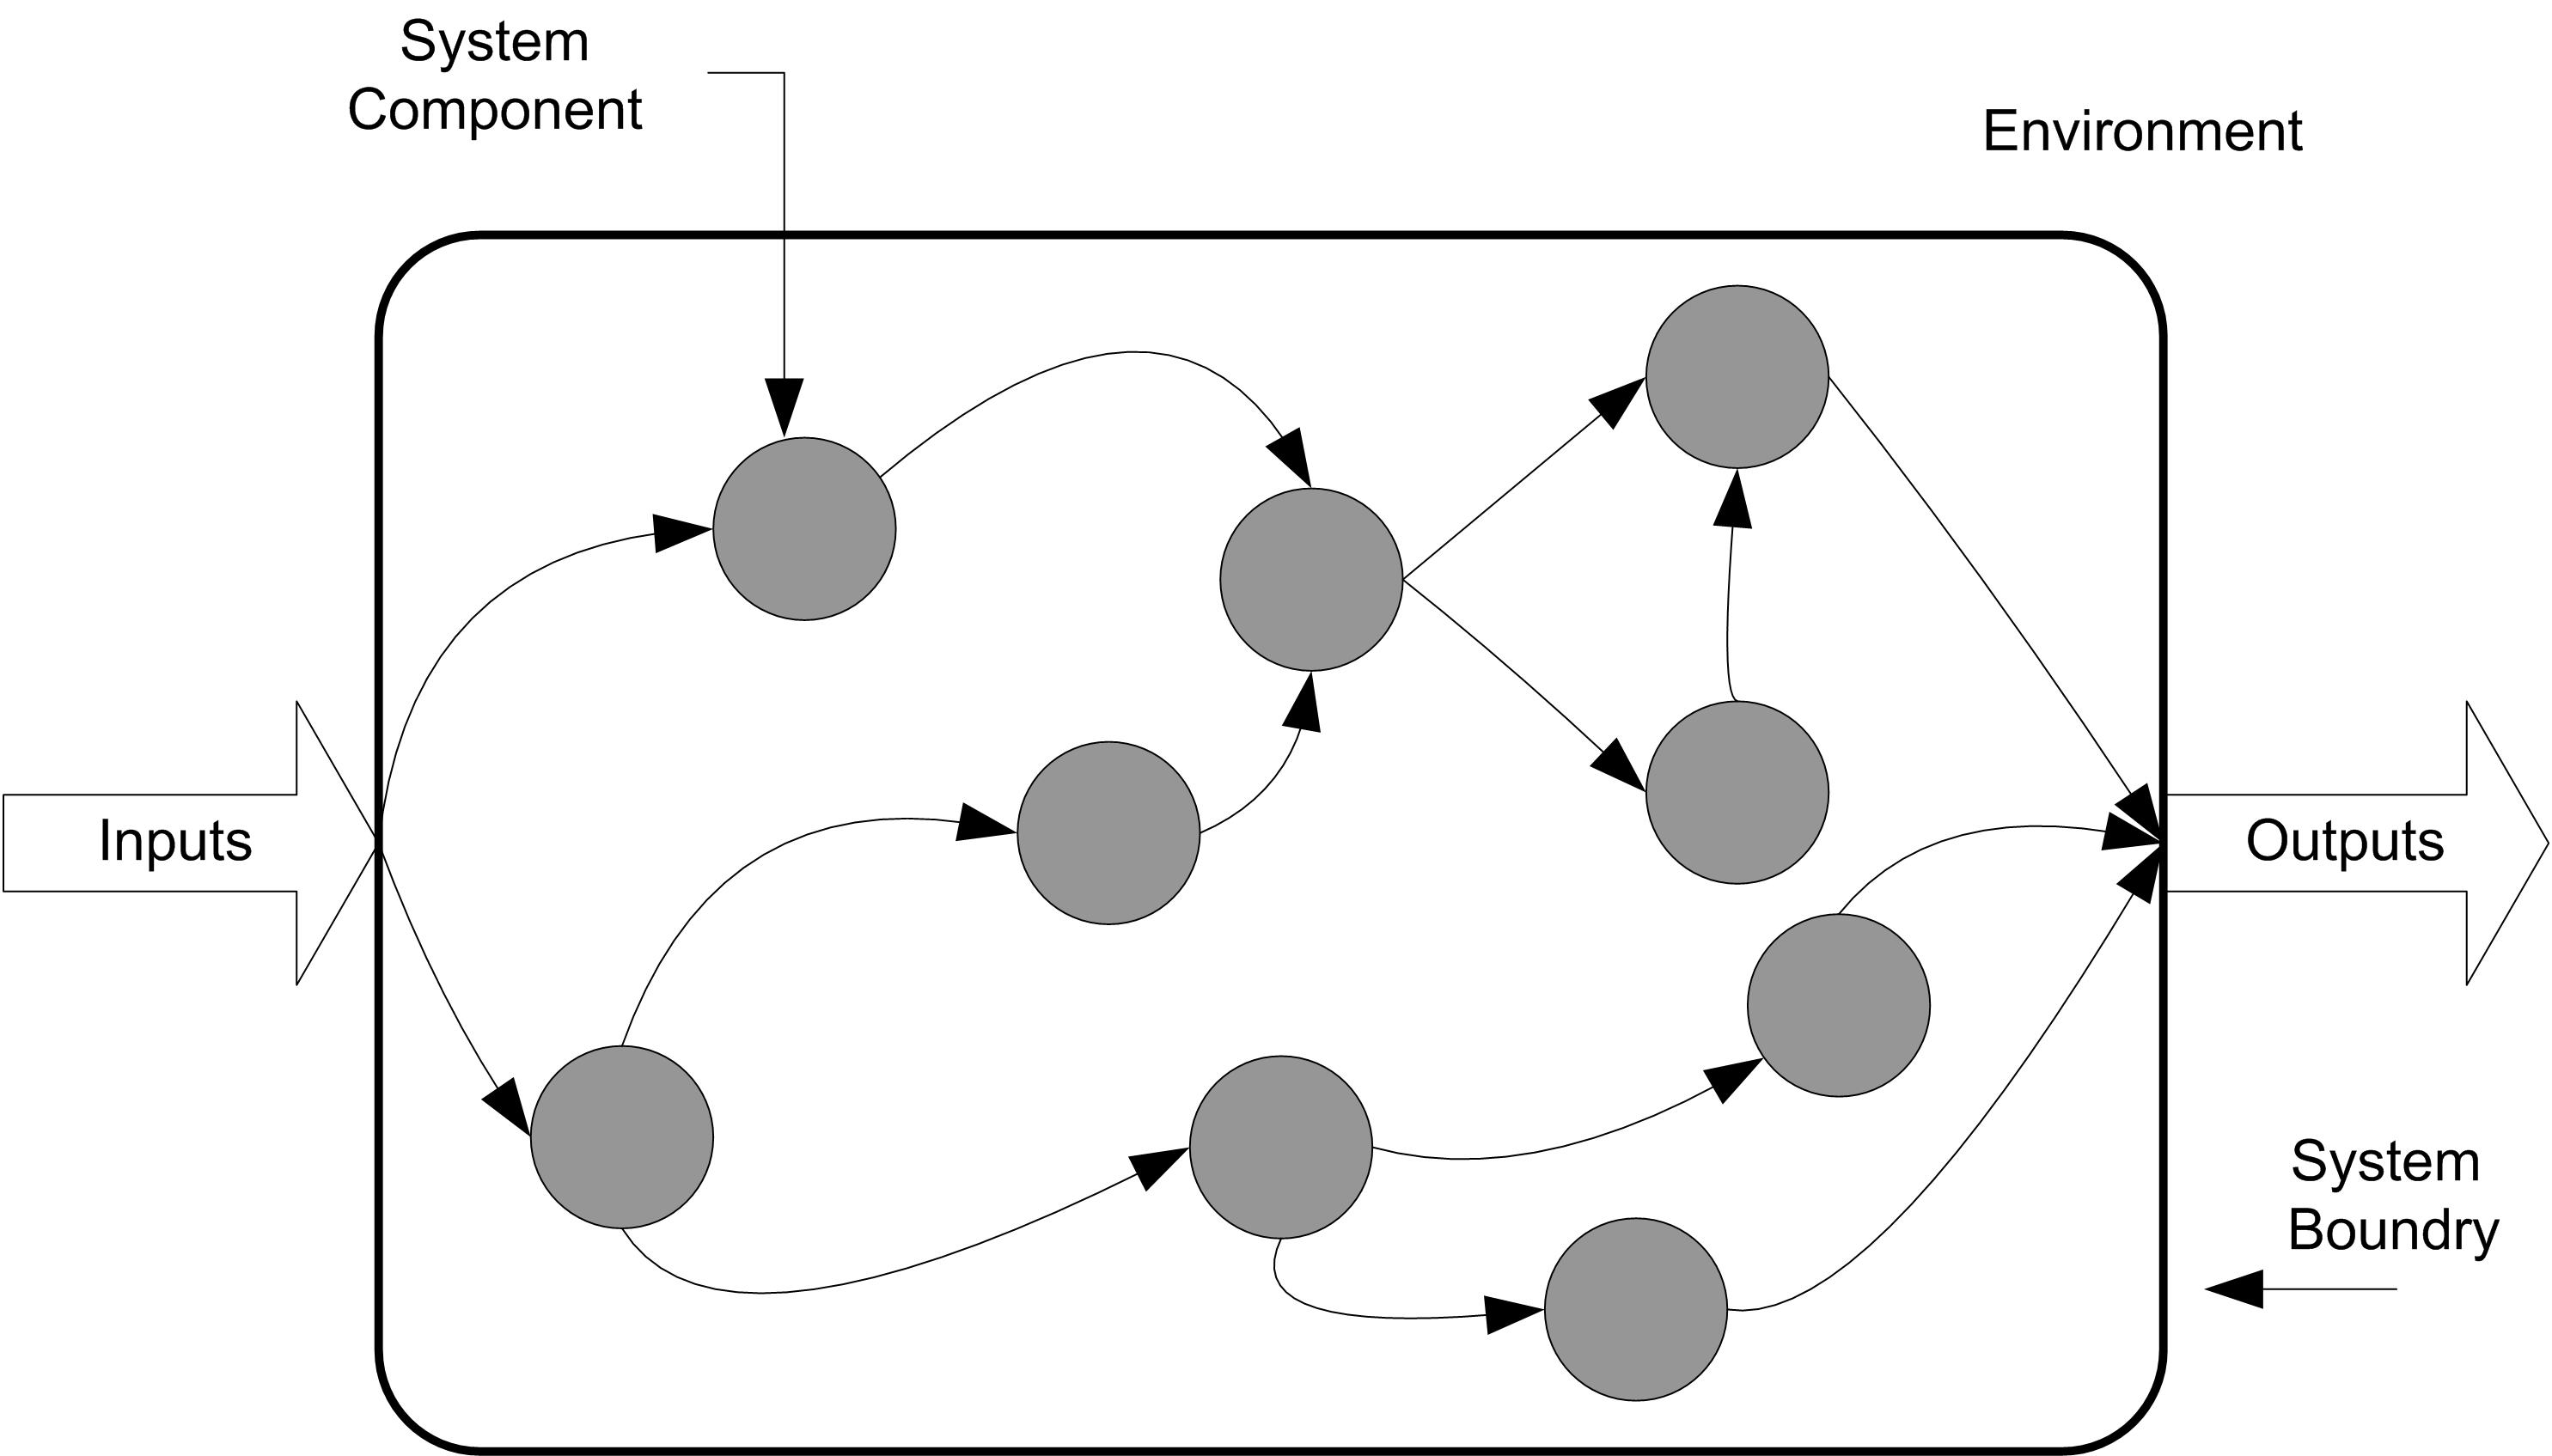
\includegraphics[width=0.9\linewidth,height=0.9\textheight]{./figures2/ch1/ch1fig1} 

}

\caption{Conceptualization of a system}\label{fig:ch1SystemConcept}
\end{figure}

Because how you conceptualize a system drives your modeling, it is
useful to discuss some general system classifications. Systems might be
classified by whether or not they are man-made (e.g.~manufacturing
system) or whether they are natural (e.g.~solar system). A system can be
physical (e.g.~an airport) or conceptual (e.g.~a system of equations).
If stochastic or random behavior is an important component of the system
then the system is said to be stochastic, if not then it is considered
deterministic. One of the more useful ways to look at a system is
whether it changes with respect to time. If a system does not change
significantly with respect to time it is said to be static, else it is
called dynamic. If a system is dynamic, you might want to consider how
it evolves with respect to time. A dynamic system is said to be discrete
if the state of the system changes at discrete points in time. A dynamic
system is said to be continuous if the state of the system changes
continuously with time. This dichotomy is purely a function of your
level of abstraction. If conceptualizing a system as discrete, serves
our purposes then you can call the system discrete.
Figure \ref{fig:ch1SystemTypes} illustrates this classification of
systems. This book primarily examines stochastic, dynamic, discrete
systems. \index{system!conceptualization} \index{system!types}

\begin{figure}

{\centering 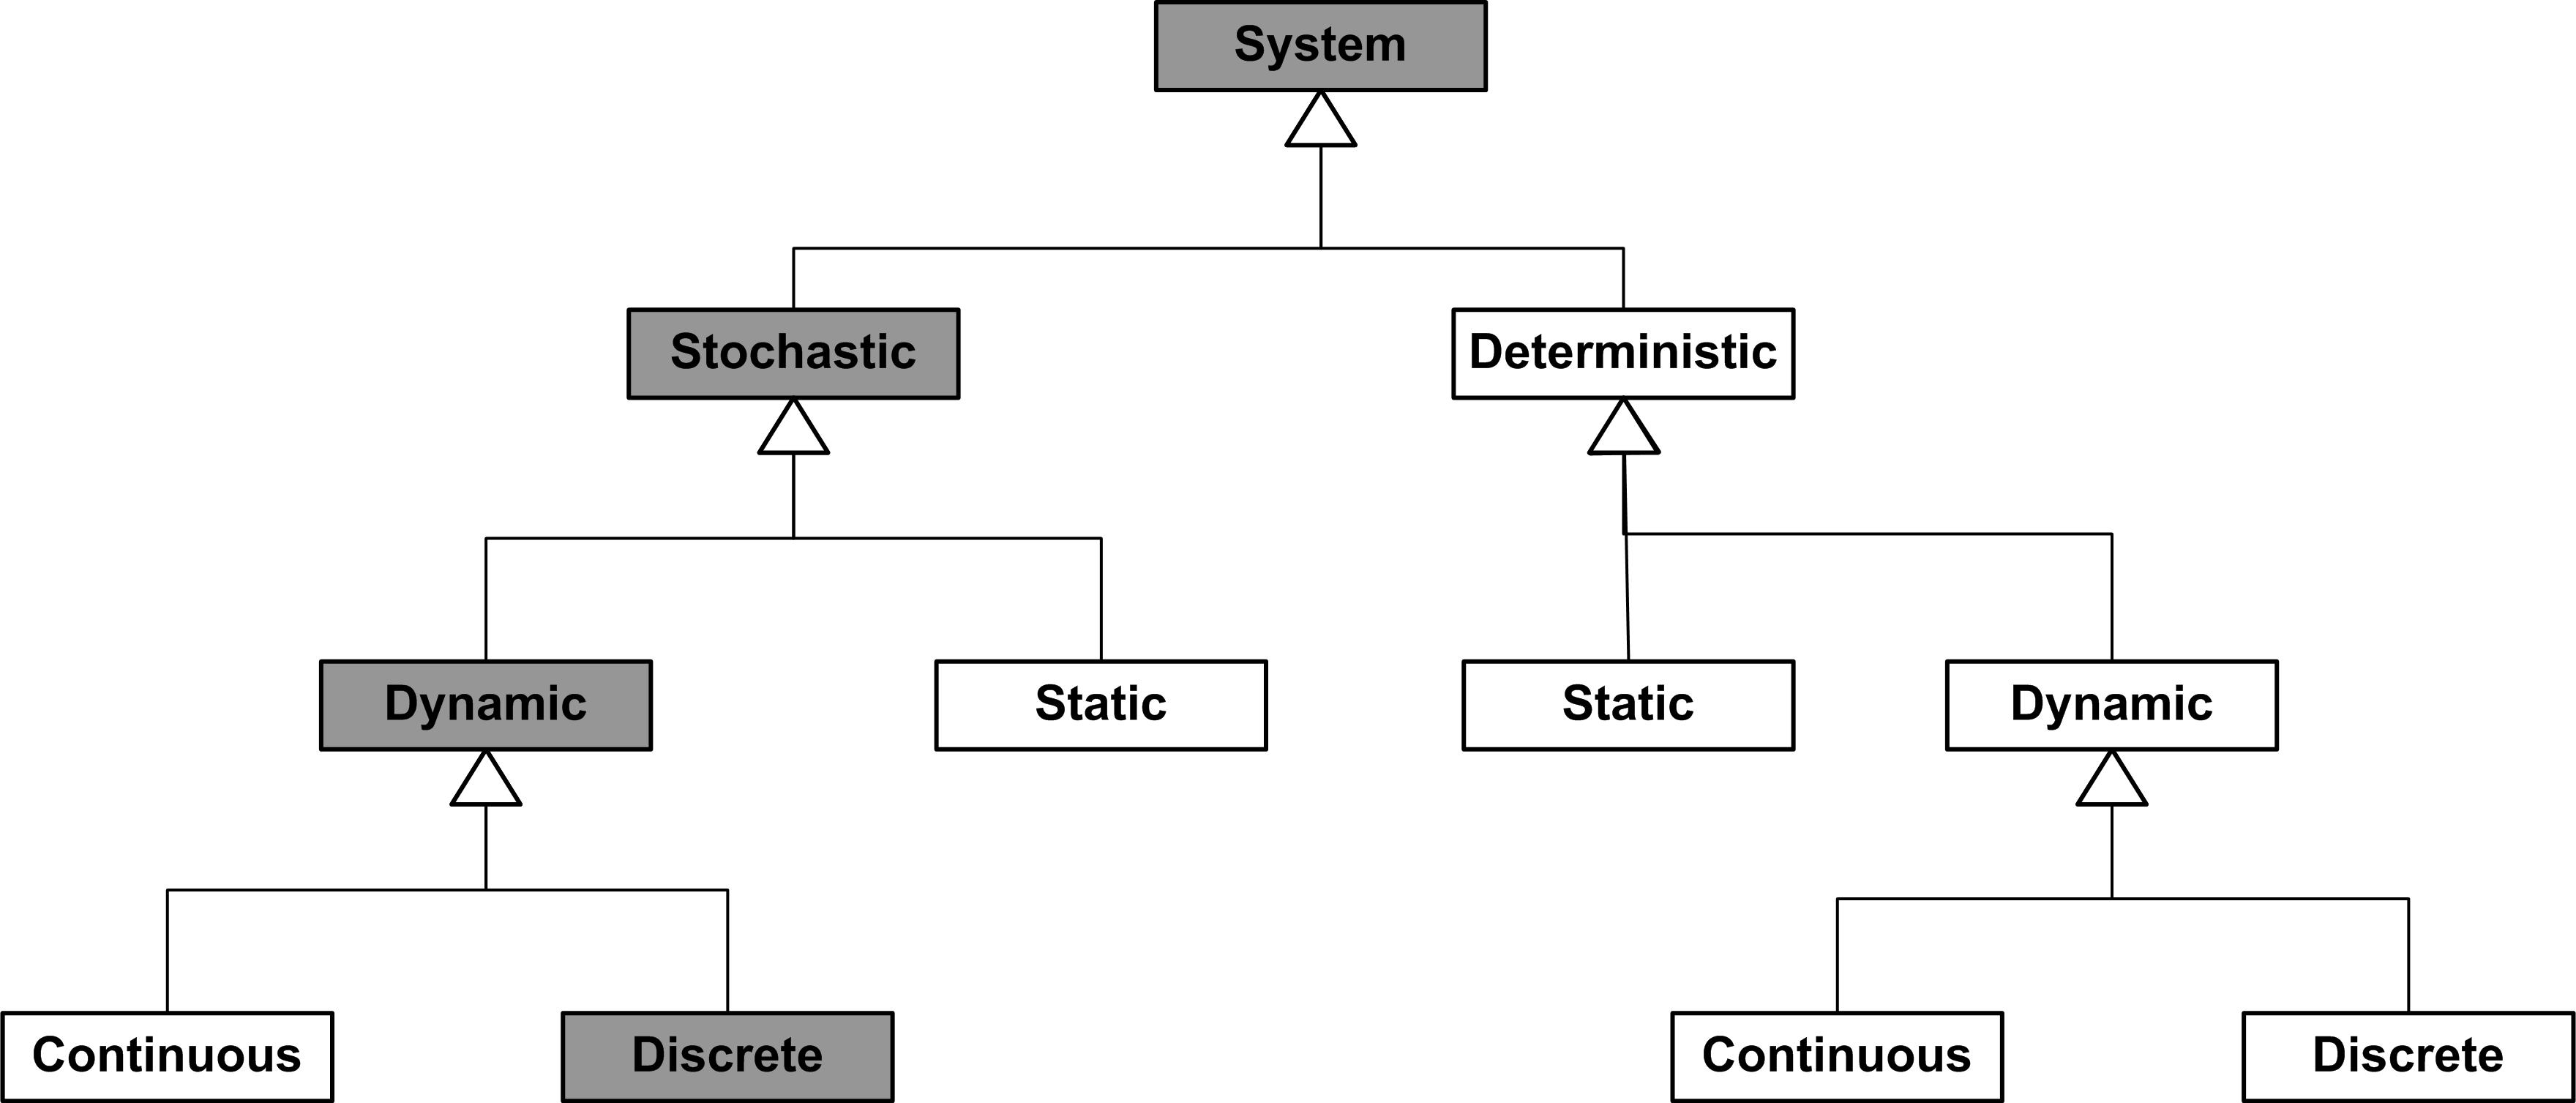
\includegraphics[width=0.9\linewidth,height=0.9\textheight]{./figures2/ch1/ch1fig2} 

}

\caption{General types of systems}\label{fig:ch1SystemTypes}
\end{figure}

\index{system!stochastic} \index{system!deterministic} \index{system!discrete} \index{system!continuous} \index{system!static} \index{system!dynamic}
The main purpose of a simulation model is to allow observations about a
particular system to be gathered as a function of time. From that
standpoint, there are two distinct types of simulation: 1) discrete
event and 2) continuous.

Just as discrete systems change at discrete points in time, in discrete
event simulation observations are gathered at selected points in time
when certain changes take place in the system. These selected points in
time are called events. On the other hand, continuous simulation
requires that observations be collected continuously at every point in
time (or at least that the system is described for all points in time).
The types of models to be examined in this book are called
discrete-event simulation models.

To illustrate the difference between the two types of simulation,
contrast a fast food service counter with that of oil loading facility
that is filling tankers. In the fast food service counter system,
changes in the status of the system occur when a customer either arrives
to place an order or when the customer receives their food. At these two
events, measures such as queue length and waiting time will be affected.
At all the other points in time, these measures remain either unchanged
(e.g.~queue length) or not yet ready for observation (e.g.~waiting time
of the customer). For this reason, the system does not need to be
observed on a continuous basis. The system need only be observed at
selected discrete points in time, resulting in the applicability of a
discrete-event simulation model.

In the case of the oil tanker loading example, one of the measures of
performance is the amount of oil in each tanker. Because the oil is a
liquid, it cannot be readily divided into discrete components. That is,
it flows continuously into the tanker. It is not necessary (or
practical) to track each molecule of oil individually, when you only
care about the level of the oil in the tanker. In this case, a model of
the system must describe the rate of flow over time and the output of
the model is presented as a function of time. Systems such as these are
often modeled using differential equations. The solution of these
equations involves numerical methods that integrate the state of the
modeled system over time. This, in essence, involves dividing time into
small equal intervals and stepping through time.\index{system!continuous}

Often both the discrete and continuous viewpoints are relevant in
modeling a system. For example, if oil tanker arrives at the port to be
filled, we have an arrival event that changes the state of the system.
This type of modeling situation is called combined continuous discrete
modeling.

A system and our resulting model depends on how we characterize the state of the system. The \textbf{state} of a system is the set of properties/variables that
describe the system at any time \(\{x_1(t), x_2(t), \dots\}\) where \(x_1(t)\) is a
variable that represents a system property value at time \(t\). Variables that take
on a countable set of values are \textbf{discrete}. Variables that take on an
uncountable set of values are said to be \textbf{continuous}. For discrete
variables, we can define a mapping from the set of integers to each
possible value. Even in the discrete case, there may be an infinite number of values. Continuous
variables are represented by the set of real numbers. That is, there are
an unaccountably infinite number of possible values that the variable can take on.
\index{system!discrete}
A discrete system has all discrete variables in its state. A continuous
system has all continuous variables in its state. A combined
continuous-discrete system has both types of variables in defining its
state. Consider an airplane:

\begin{itemize}
\item
  If we are interested in the number of parts operating to
  specification at any time t, then the state is \(\{N_1(t), N_2(t), \dots \}\)
  where \(N_1(t) = 1\) if part 1 is operating and 0 if part 1 is not
  operating to specification. The state vector consists of all
  discrete variables. This is a discrete system.
\item
  If we are interested in the temperature of each part at time \(t\), then
  the state is \(\{T_1(t), T_2(t), \dots \}\), where \(T_1(t)\) is the temperature
  in Celsius of part 1 at time \(t\), etc. The state vector consists of
  all continuous variables. This is continuous system.
\item
  If we are interested in the velocity of a plane at time \(t\) and the
  number of wheels deployed at time \(t\), then the state is \(\{v(t), n(t)\}\)
  where \(v(t)\) is the velocity of the plane in meters/second and \(n(t)\) is
  \(\{0,1,2,3,4\}\) wheels. Then the state vector consists of both
  continuous and discrete variables that change with time. This is a
  combined continuous/discrete system.
\end{itemize}

Static systems are systems for which time is not a significant factor. In other words, that the
state does not evolve over time. Dynamic systems are systems for which
system state changes with respect to time. In a deterministic system, the variables
are not governed by underlying random processes. In a stochastic
system, some of the variables are governed by underlying random
processes. Time can change continuously or at discrete points. When time
changes only at discrete points in time, we call these points, events.

Some simulation languages have modeling constructs for both
continuous and discrete modeling; however, this book does not cover the
modeling of continuous or combined continuous discrete systems. There are
many useful references on this topic. We will be modeling discrete-event dynamic stochastic systems in this textbook.

\hypertarget{simulation-descriptive-or-prescriptive-modeling}{%
\section{Simulation: Descriptive or Prescriptive Modeling?}\label{simulation-descriptive-or-prescriptive-modeling}}

A descriptive model describes how a system behaves. Simulation is at its
heart a descriptive modeling technique. Simulation is used to depict the
behaviors or characteristics of existing or proposed systems. However, a
key use of simulation is to convey the \emph{required} behaviors or
properties of a proposed system. In this situation, simulation is used
to prescribe a solution. A prescriptive model tells us what to do. In
other words, simulation can also be used for prescriptive modeling.
Figure \ref{fig:ch1PrescriptiveSimulation} illustrates the concept of
using simulation to recommend a solution.

\begin{figure}

{\centering 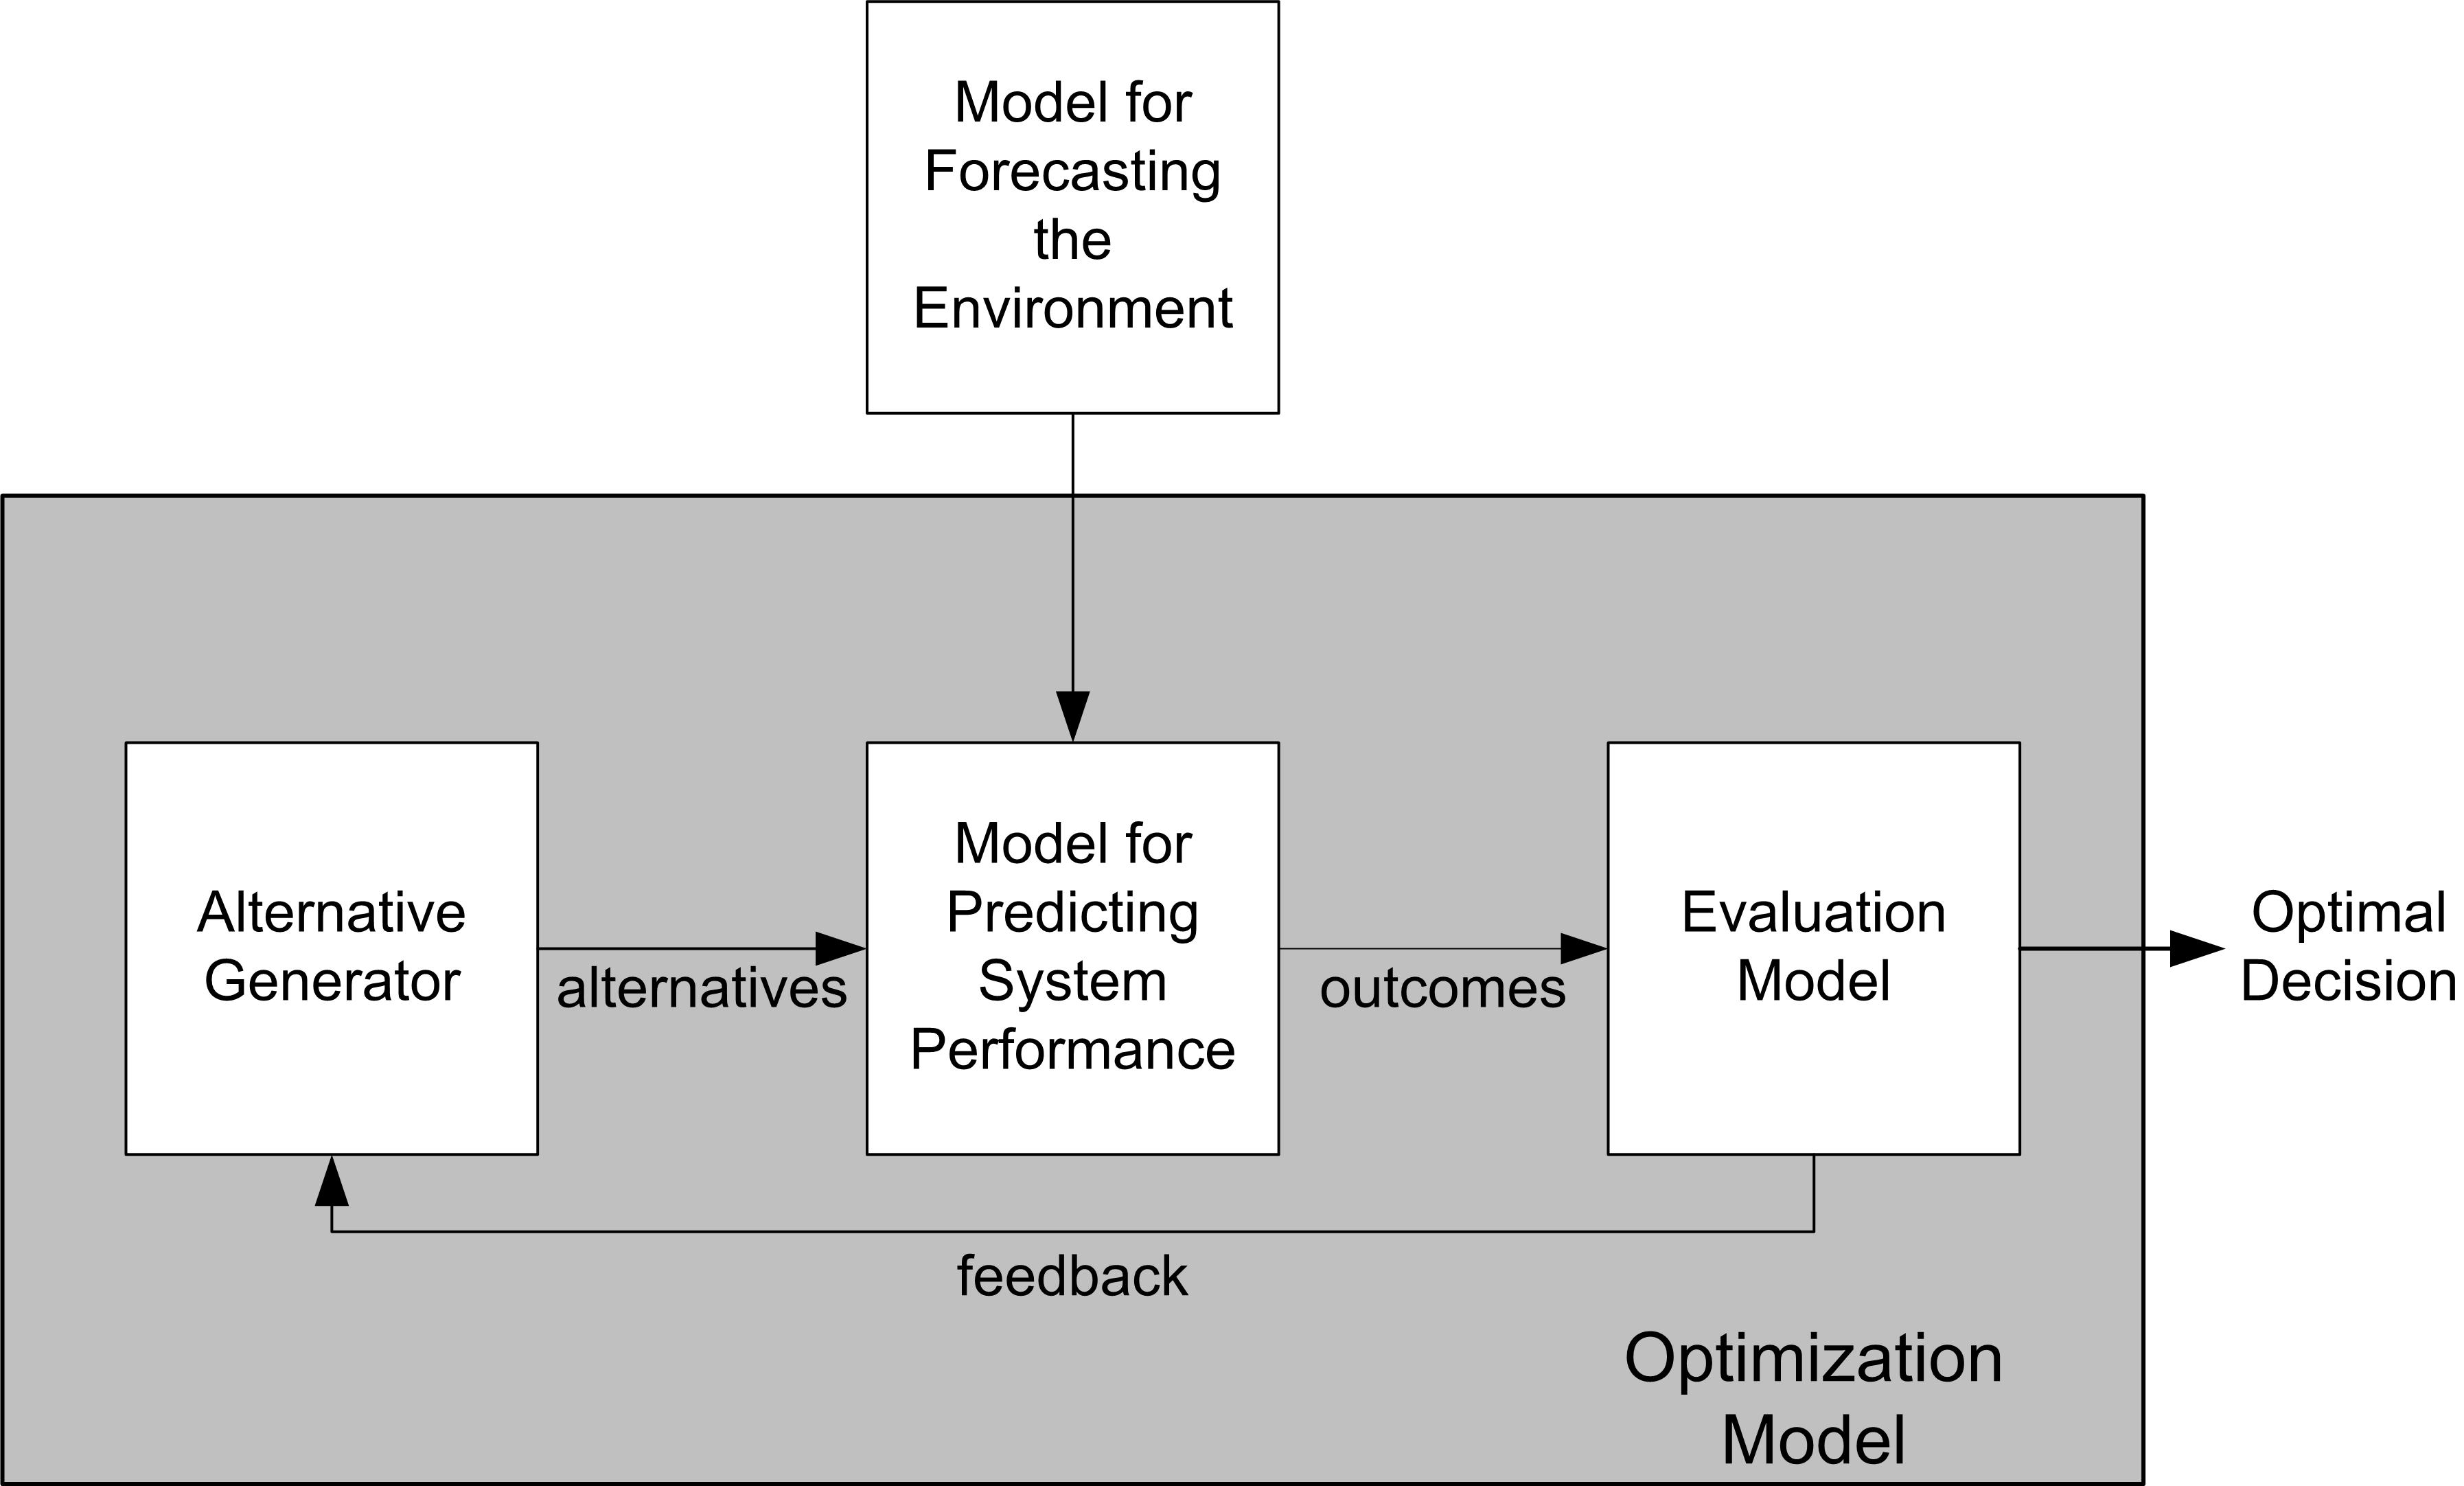
\includegraphics[width=0.9\linewidth,height=0.9\textheight]{./figures2/ch1/ch1fig3} 

}

\caption{Using simulation for prescriptive analysis}\label{fig:ch1PrescriptiveSimulation}
\end{figure}

\index{model!descriptive} \index{model!prescriptive} \index{model!predictive}
In the figure, a simulation model is used for predicting the behavior of
the system. Input models are used to characterize the system and its
environment. An evaluative model is used to evaluate the output of the
simulation model to understand how the output compares to desired goals.
The alternative generator is used to generate different scenarios to be
feed into the simulation model for evaluation. Through a feedback
mechanism the inputs can be changed based on the evaluation of the
outputs and eventually a recommended solution can be achieved.

For example, in the modeling a drive up pharmacy, suppose that the
probability of a customer waiting longer than 3 minutes in line had to
be less than 10\%. To form design alternatives, the inputs (e.g.~number
of pharmacists, possibly the service process) can be varied. Each
alternative can then be evaluated to see if the waiting time criteria is
met. In this simple situation, you might act as your own alternative
generator and the evaluative model is as simple as meeting a criteria;
however, in more complex models, there will often be hundreds of inputs
to vary and multiple competing objectives. In such situations,
simulation optimization and heuristic search methods are often used.
This is an active and important area of research within simulation.

\hypertarget{randomness-in-simulation}{%
\section{Randomness in Simulation}\label{randomness-in-simulation}}

\index{randomness}
In most real-life situations, the arrival process and the service
process occur in a random fashion. Even though the processes may be
random, it does not mean that you cannot describe or model the
randomness. To have any hope of simulating the situation, you must be
able to model the randomness. One of the ways to model this randomness
is to describe the phenomenon as a random variable governed by a
particular probability distribution. For example, if the arrivals to the
bank occur according to a Poisson process, then from probability theory
it is known that the distribution of inter-arrival times is an
exponential distribution. In general, information about how the
customers arrive must be secured either through direct observation of
the system or by using historical data. If neither source of information
is available, then some plausible assumptions must be made to describe
the random process by a probability model.

If historical data is available, there are two basic choices for how to
handle the modeling. The first choice is to develop a probability model
given the data. The second choice is to try to drive the simulation
directly from the historical data. The latter approach is not
recommended. First of all, it is extremely unlikely that the captured
data will be in a directly usable form. Secondly, it is even more
unlikely that the data will be able to adequately represent all the
modeling scenarios that you will need through the course of
experimenting with the model. For example, suppose that you only have 1
day's worth of arrival data, but you need to simulate a month's worth of
system operation. If you simply re-drive your simulation using the 1
day's worth of data, you are not simulating different days! It is much
more advisable to develop probability models either from historical data
or from data that you capture in developing your model. Appendix \ref{app:idm}
discusses some of the tools and techniques for modeling probability
distributions.

Once a probability model has been developed, statistical theory provides
the means for obtaining random samples based on the use of uniformly
distributed random numbers on the interval (0,1). These random samples
are then used to map the future occurrence of an event on the time
scale. For example, if the inter-arrival time is exponential then a
random sample drawn from that distribution would represent the time
interval until the occurrence of the next arrival. The process of
generating random numbers and random variables within simulation is
presented in Appendix \ref{app:rnrv}.

\hypertarget{simulation-languages}{%
\section{Simulation Languages}\label{simulation-languages}}

\index{simulation!languages}
Discrete event simulation normally involves a tremendous volume of
computation. Consequently, the use of computers to carry out these
computations is essential; however, the volume of computations is not
the only obstacle in simulation. If you consider the bank teller example
discussed in the previous sections, you will discover that it involves a
complex logical structure that requires special expertise before it can
be translated into a computer model. Attempting to implement the
simulation model, from scratch, in a general purpose language such as
FORTRAN, Visual Basic, C/C++, or Java will require above average
programming skills. In the absence of specialized libraries for these
languages that try to relieve the user from some of the burden,
simulation as a tool would be relegated to "elite" programmers.
Luckily, the repetitive nature of computations in simulation allows the
development of computer libraries that are applicable to simulation
modeling situations. For example, libraries or packages must be
available for ordering and processing events chronologically, as well as
generating random numbers and automatically collecting statistics. Such
a \href{https://git.uark.edu/jslfork/JSL}{library} for simulating discrete-event systems in Java is available from the author, see \citep{Rossetti2008aa} and the related \href{https://rossetti.git-pages.uark.edu/jslbookdownbook/}{book}.

The computational power and storage capacity of computers has motivated
the development of specialized simulation languages. Some languages have
been developed for continuous or discrete simulations. Others can be
used for combined continuous and discrete modeling. All simulation
languages provide certain standard programming facilities and will
differ in how the user will take advantage of these facilities. There is
normally some trade-off between how flexible the language is in
representing certain modeling situations. Usually, languages that are
highly flexible in representing complex situations require more work
(and care) by the user to account for how the model logic is developed.
Some languages are more programming oriented (e.g.~SIMSCRIPT) and others
are more "drag and drop" (e.g.~ProModel, Arena, etc. ).

The choice of a simulation language is a difficult one. There are many
competing languages, each having their own advantages and disadvantages.
The Institute for Operations Research and Management Science (INFORMS)
often has a yearly product review covering commercial simulation
languages, see for example (\url{http://lionhrtpub.com/orms/}). In addition to
this useful comparison, you should examine the Winter Simulation
Conference (www.wintersim.org). The conference has hands on exhibits of
simulation software and the conference proceedings often have tutorials
for the various software packages. Past proceedings have been made
available electronically through the generous support of the INFORMS
Society for Simulation (\url{http://www.informs-sim.org/wscpapers.html}).

was chosen for this textbook because of the author's experience
utilizing the software, its ease of use, and the availability of student
versions of the software. While all languages have flaws, using a
simulation language is essential in performing high performance
simulation studies. Most, if not all simulation companies have strong
support to assist the user in learning their software. has a strong
academic and industrial user base and is very competitive in the
simulation marketplace. Once you learn one simulation language well, it
is much easier to switch to other languages and to understand which
languages will be more appropriate for certain modeling situations.

is fundamentally a process description based language. That is, when
using , the modeler describes the process that an "entity" experiences
while flowing through or using the elements of the system. You will
learn about how facilitates process modeling throughout this textbook.

\hypertarget{ch1:sec:simMeth}{%
\section{Simulation Methodology}\label{ch1:sec:simMeth}}

\index{simulation!methodology}
This section presents a brief overview of the steps of simulation
modeling by discussing the process in the context of a methodology. A
methodology is simply a series of steps to follow. Since simulation
involves systems modeling, a simulation methodology based on the general
precepts of solving a problem through systems analysis is presented
here. A general methodology for solving problems can be stated as
follows: \index{DEGREE}

\begin{enumerate}
\def\labelenumi{\arabic{enumi}.}
\item
  Define the problem
\item
  Establish measures of performance for evaluation
\item
  Generate alternative solutions
\item
  Rank alternative solutions
\item
  Evaluate and Iterate during process \index{iteration}
\item
  Execute and evaluate the solution
\end{enumerate}

This methodology can be referred to by using the first letter of each
step. The DEGREE methodology for problem solving represents a series of
steps that can be used during the problem solving process. The first
step helps to ensure that you are solving the right problem. The second
step helps to ensure that you are solving the problem for the right
reason, i.e.~your metrics must be coherent with your problem. Steps 3
and 4 ensure that the analyst looks at and evaluates multiple solutions
to the problem. In other words, these steps help to ensure that you
develop the right solution to the problem. A good methodology recognizes
that the analyst needs to evaluate how well the methodology is doing. In
step 5, the analyst evaluates how the process is proceeding and allows
for iteration. Iteration is an important concept that is foreign to many
modelers. The concept of iteration recognizes that the problem solving
process can be repeated until the desired degree of modeling fidelity
has been achieved. Start the modeling at a level that allows it to be
initiated and do not try to address the entire situation in each of the
steps. Start with small models that work and build them up until you
have reached your desired goals. It is important to get started and get
something established on each step and continually go back in order to
ensure that the model is representing reality in the way that you
intended. The final step is often over looked. Simulation is often used
to recommend a solution to a problem. Step 6 indicates that if you have
the opportunity you should execute the solution by implementing the
decisions. Finally, you should always follow up to ensure that the
projected benefits of the solution were obtained.

The DEGREE problem solving methodology should serve you well; however,
simulation involves certain unique actions that must be performed during
the general overall problem solving process. When applying DEGREE to a
problem that may require simulation, the general DEGREE approach needs
to be modified to explicitly consider how simulation will interact with
the overall problem solving process.

Figure \ref{fig:ch1SimMethodology} represents a refined general
methodology for applying simulation to problem solving.

\begin{enumerate}
\def\labelenumi{\arabic{enumi}.}
\item
  Problem Formulation \index{problem formulation}

  \begin{enumerate}
  \def\labelenumii{\arabic{enumii}.}
  \item
    Define the problem
  \item
    Define the system
  \item
    Establish performance metrics
  \item
    Build conceptual model
  \item
    Document model assumptions
  \end{enumerate}
\item
  Simulation Model Building

  \begin{enumerate}
  \def\labelenumii{\arabic{enumii}.}
  \item
    Model translation
  \item
    Input data modeling
  \item
    Verification \index{verification}
  \item
    Validation \index{validation}
  \end{enumerate}
\item
  Experimental Design and Analysis \index{experimental design}

  \begin{enumerate}
  \def\labelenumii{\arabic{enumii}.}
  \item
    Preliminary Runs
  \item
    Final experiments
  \item
    Analysis of results
  \end{enumerate}
\item
  Evaluate and Iterate

  \begin{enumerate}
  \def\labelenumii{\arabic{enumii}.}
  \item
    Documentation
  \item
    Model manual
  \item
    User manual
  \end{enumerate}
\item
  Implementation
  \index{problem formulation}
  The first phase, problem formulation, captures the essence of the first
  two steps in the DEGREE process. The second phase, model building,
  captures the essence of step 3 of the DEGREE process. When building
  models, you are either explicitly or implicitly developing certain
  design alternatives. The third phase, experimental design and analysis,
  encapsulates some of steps 3 and 4 of the DEGREE process. In designing
  experiments, design alternatives are specified and when analyzing
  experiments their worth is being evaluated with respect to problem
  objectives. The fourth phase, evaluate and iterate, captures the notion
  of iteration. Finally, the fifth and sixth phases, documentation and
  implementation complete the simulation process. Documentation is
  essential when trying to ensure the ongoing and future use of the
  simulation model, and implementation recognizes that simulation projects
  often fail if there is no follow through on the recommended solutions.
\end{enumerate}

\begin{figure}

{\centering 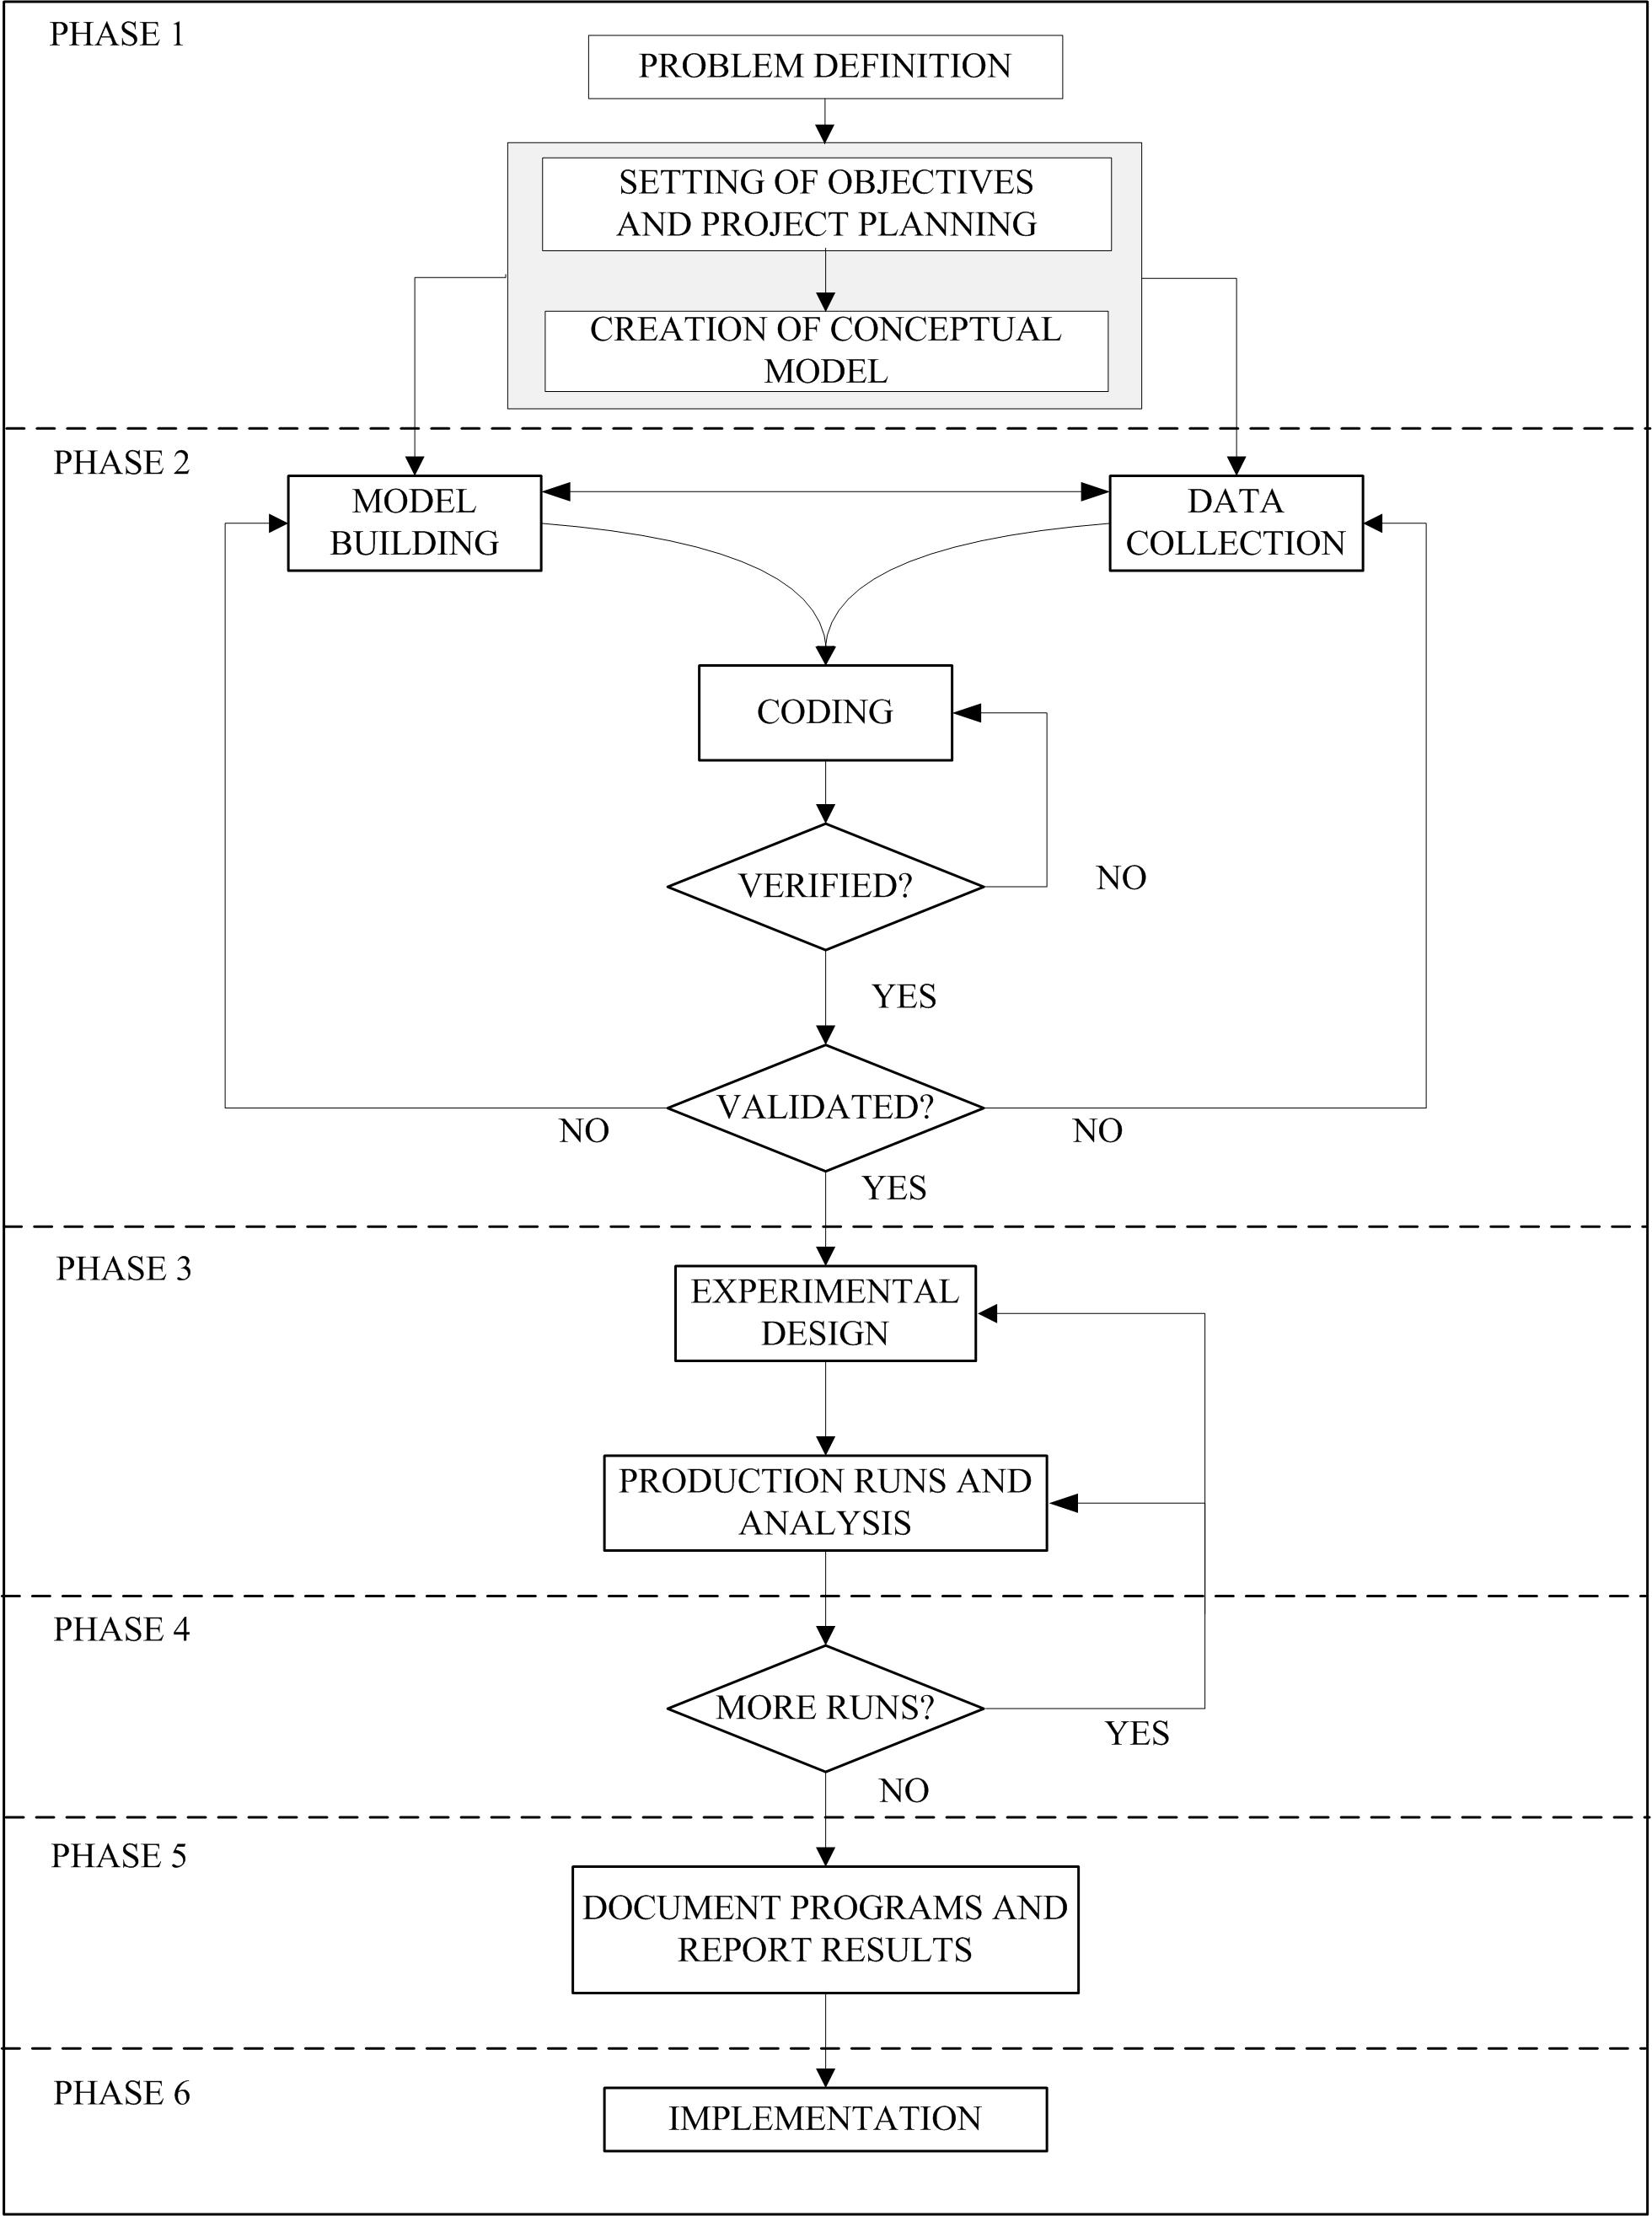
\includegraphics[width=0.9\linewidth,height=0.9\textheight]{./figures2/ch1/ch1fig4} 

}

\caption{General simulation project methodology}\label{fig:ch1SimMethodology}
\end{figure}

The problem formulation phase of the study consists of five primary
activities:

\begin{enumerate}
\def\labelenumi{\arabic{enumi}.}
\item
  Defining the problem
\item
  Defining the system
\item
  Establishing performance metrics.
\item
  Building conceptual models
\item
  Documenting modeling assumptions
\end{enumerate}

A problem starts with a perceived need. These activities are useful in
developing an appreciation for and an understanding of what needs to be
solved. The basic output of the problem definition activity is a problem
definition statement. A problem definition statement is a narrative
discussion of the problem. A problem definition statement is necessary
to accurately and concisely represent the problem for the analyst and
for the problem stakeholders. This should include all the required
assumptions made during the modeling process. It is important to
document your assumptions so that you can examine their effect on the
model during the verification, validation, and experimental analysis
steps of the methodology. This ensures that the problem is well
understood and that all parties agree upon the nature of the problem and
the goals of the study. The general goals of a simulation study often
include:

\begin{itemize}
\item
  Comparison: To compare system alternatives and their performance
  measures across various factors (decision variables) with respect to
  some objectives
\item
  Optimization: This is a special case of comparison in which you try
  to find the system configuration that optimizes performance subject
  to constraints.
\item
  Prediction: To predict the behavior of the system at some future
  point in time.
\item
  Investigation: To learn about and gain insight into the behavior of
  the system given various inputs.
\end{itemize}

These general goals will need to be specialized to the problem under
study. The problem definition should include a detailed description of
the objectives of the study, the desired outputs from the model, and the
types of scenarios to be examined or decisions to be made.
\index{system!definition}
The second activity of this phase produces a definition of the system. A
system definition statement is necessary to accurately and concisely
define the system, particularly its boundaries. The system definition
statement is a narrative, which often contains a pictorial
representation of the major elements of the system. This ensures that
the simulation study is focused on the appropriate areas of interest to
the stakeholders and that the scope of the project is well understood.

When defining the problem and the system, one should naturally begin to
develop an understanding of how to measure system performance. The third
activity of problem formulation makes this explicit by encouraging the
analyst to define the required performance measures for the model. To
meaningfully compare alternative scenarios, objective and measurable
metrics describing the performance of the system are necessary. The
performance metrics should include quantitative statistical measures
from any models used in the analysis (e.g.~simulation models),
quantitative measures from the systems analysis, (e.g.~cost/benefits),
and qualitative assessments (e.g.~technical feasibility, human,
operational feasibility). The focus should be placed on the performance
measures that are considered to be the most important to system
decision-makers and tied directly to the objectives of the simulation
study. Evaluation of alternatives can then proceed in an objective and
unbiased manner to determine which system scenario performs the best
according to the decision maker's preferences.

The problem definition statement, the system definition statement, and
explicit performance metrics set the stage for more detailed modeling.
These activities should be captured in a written form. Within this text,
you will develop models of certain ``ready-made'' book problems. One way
to accomplish the problem formulation phase of a simulation study is to
consider writing yourself a "book problem". You will need enough
detail in these documents that a simulation analyst (you) can develop a
model in any simulation language for the given situation. The example
problem in Chapter \ref{ch8} represents an excellent sample of problem and system
definition statements. If you have the opportunity to do a ``real-life''
project as part of your study of simulation, you might want to utilize
the book problems in this text and the example in
Chapter \ref{ch8} for how
to write reasonable problem/system definition statements.

With a good understanding of the problem and of the system under study,
you should be ready to begin your detailed model formulations. Model
formulation does not mean a computer program. You should instead use
conceptual modeling tools: conceptual diagrams, flow charts, etc. prior
to any use of software to implement a model. The purpose of conceptual
modeling tools is to convey a more detailed system description so that
the model may be translated into a computer representation. General
descriptions help to highlight the areas and processes of the system
that the model will simulate. Detailed descriptions assist in simulation
model development and coding efforts. Some relevant diagramming
constructs include:

\begin{enumerate}
\def\labelenumi{\arabic{enumi}.}
\item
  Context Diagrams: A context diagram assists in conveying the general
  system description. The diagram is a pictorial representation of the
  system that often includes flow patterns typically encountered.
  Context diagrams are often part of the system description document.
  There are no rules for developing context diagrams. If you have an
  artistic side, here is your opportunity to shine!
\item
  Activity Diagrams: An activity diagram is a pictorial representation
  of the process for an entity and its interaction with resources
  while within the system. If the entity is a temporary entity (i.e.
  it flows through the system) the activity diagram is called an
  activity flow diagram. If the entity is permanent (i.e.~it remains
  in the system throughout its life) the activity diagram is called an
  activity cycle diagram. Activity diagrams will be used extensively
  within this text. \index{activity diagram}
\item
  Software engineering diagrams: Because simulation entails software
  development, the wide-variety of software engineering diagramming
  techniques can be utilized to provide information for the model
  builder. Diagrams such as flow charts, database diagrams, IDEF (ICAM
  DEFinition language) diagrams, UML (unified modeling language)
  diagrams, state charts, etc are all useful in documenting complex
  modeling situations. These techniques assist development and coding
  efforts by focusing attention on describing, and thus understanding,
  the elements within the system. Within this text, activity diagrams
  will be augmented with some simple flow chart symbols and some
  simple state diagrams will be used to illustrate a variety of
  concepts.
\end{enumerate}

In your modeling, you should start with an easy conceptual model that
captures the basic aspects and behaviors of the system. Then, you should
begin to add details, considering additional functionality. Finally, you
should always remember that the complexity of the model has to remain
proportional to the quality of the available data and the degree of
validity necessary to meet the objectives of the study. In other words,
don't try to model the world! \index{conceptual model}

After developing a solid conceptual model of the situation, simulation
model building can begin. During the simulation model building phase,
alternative system design configurations are developed based on the
previously developed conceptual models. Additional project planning is
also performed to yield specifications for the equipment, resources, and
timing required for the development of the simulation models. The
simulation models used to evaluate the alternative solutions are then
developed, verified, validated, and prepared for analysis. Within the
context of a simulation project this process includes:

\begin{itemize}
\item
  Input Data Preparation: Input data is analyzed to determine the
  nature of the data and to determine further data collection needs.
  Necessary data is also classified into several areas. This
  classification establishes different aspects of the model that are
  used in model development.
\item
  Model Translation: Description of the procedure for coding the
  model, including timing and general procedures and the translation
  of the conceptual models into computer simulation program
  representations.
\item
  Verification: Verification of the computer simulation model is
  performed to determine whether or not the program performs as
  intended. To perform model verification, model debugging is
  performed to locate any errors in the simulation code. Errors of
  particular importance include improper flow control or entity
  creation, failure to release resources, and logical/arithmetic
  errors or incorrectly observed statistics. Model debugging also
  includes scenario repetition utilizing identical random number
  seeds, "stressing" the model through a sensitivity analysis
  (varying factors and their levels) to ensure compliance with
  anticipated behavior, and testing of individual modules within the
  simulation code. \index{verification}
\item
  Validation: Validation of the simulation model is performed to
  determine whether or not the simulation model adequately represents
  the real system. The simulation model is shown to personnel (of
  various levels) associated with the system in question. Their input
  concerning the realism of the model is critical in establishing the
  validity of the simulation. In addition, further observations of the
  system are performed to ensure model validity with respect to actual
  system performance. A simple technique is to statistically compare
  the output of the simulation model to the output from the real
  system and to analyze whether there is a significant (and practical)
  difference between the two. \index{validation}
  \index{model translation}
  Model translation will be a large component of each chapter as you learn
  how to develop simulation models. Verification and validation techniques
  will not be a major component of this text, primarily because the models
  will be examples made for educational purposes. This does not mean that
  you should ignore this important topic. You are encouraged to examine
  many of the useful references on validation, see for example
  \citep{balci1997principles} and \citep{balci1998verification}.
\end{itemize}

After you are confident that your model has been verified and validated
to suit your purposes, you can begin to use the model to perform
experiments that investigate the goals and objectives of the project.
Preliminary simulation experiments should be performed to set the
statistical parameters associated with the main experimental study. The
experimental method should use the simulation model to generate
benchmark statistics of current system operations. The simulation model
is then altered to conform to a potential scenario and is re-run to
generate comparative statistics. This process is continued, cycling
through suggested scenarios and generating comparative statistics to
allow evaluation of alternative solutions. In this manner, objective
assessments of alternative scenarios can be made.

For a small set of alternatives, this ``one at a time'' approach is
reasonable; however, often there are a significant number of design
factors that can affect the performance of the model. In this situation,
the analyst should consider utilizing formal experimental design
techniques. This step should include a detailed specification of the
experimental design (e.g.~factorial, etc) and any advanced output
analysis techniques (e.g.~batching, initialization bias prevention,
variance reduction techniques, multiple comparison procedures, etc.)
that may be required during the execution of the experiments. During
this step of the process, any quantitative models developed during the
previous steps are exercised. Within the context of a simulation
project, the computer simulation model is exercised at each of the
design points within the stipulated experimental design.

Utilizing the criteria specified by system decision-makers, and
utilizing the simulation model's statistical results, alternative
scenarios should then be analyzed and ranked. A methodology should be
used to allow the comparison of the scenarios that have multiple
performance measures that trade-off against each other. \index{trade-off}

If you are satisfied that the simulation has achieved your objectives
then you should document and implement the recommended solutions. If
not, you can iterate as necessary and determine if any additional data,
models, experimentation, or analysis is needed to achieve your modeling
objectives. Good documentation should consist of at least two parts: a
technical manual, which can be used by the same analyst or by other
analysts, and a user manual. A good technical manual is very useful when
the project has to be modified, and it can be a very important
contribution to software reusability and portability. The approach to
documenting the example models in this text can be used as an example
for how to document your models. In addition to good model development
documentation, often the simulation model will be used by non-analysts.
In this situation, a good user manual for how to use and exercise the
model is imperative. The user manual is a product for the user who may
not be an expert in programming or simulation issues; therefore
clearness and simplicity should be its main characteristics. If within
the scope of the project, the analyst should also develop implementation
plans and follow through with the installation and integration of the
proposed solutions. After implementation, the project should be
evaluated as to whether or not the proposed solution met the intended
objectives.

\hypertarget{organization-of-the-book-1}{%
\section{Organization of the Book}\label{organization-of-the-book-1}}

This chapter introduced some of the basic concepts in simulation. Chapter \ref{ch2} will begin our exploration of discrete event simulation and introduce you to the key modeling tool, Arena. Chapter \ref{ch3} introduces the basic statistical concepts that you will need to begin to understand output generated from a simulation. Chapter \ref{ch4} presents intermediate process modeling within Arena. After these first four chapters, you will have a solid understanding of how to apply Arena to model many realistic situations via simulation. Then, Chapter \ref{ch5} returns to a statistical concept within simulation in order to prepare you to analyze the results of a infinite horizon simulation. Chapter \ref{ch6} presents more advanced process modeling, including an introduction to modeling non-stationary situations. Chapter \ref{ch7} includes the modeling of material handling and movement of within a system. Finally, Chapter \ref{ch8}, the final chapter, illustrates the use of simulation on a practical case
study. Through this study you will have a solid foundation for
understanding what it takes to model more realistic systems found in
practice.

Along with the basic modeling chapters a number of useful appendices have been provided. Appendix \ref{app:rnrv} presents the mathematical basis for random number generation and for generating random variables from probability distributions. Appendix \ref{app:idm} describes the basic processes for fitting probability distributions. Because simulation often involves the modeling of waiting systems, Appendix \ref{app:qtAndInvT} provides an overview of the analytical analysis of single queue systems and many of the important formulas that an analyst may need, especially if they use queueing theory to verify and validate their simulation models. A number of other useful appendices are provided to cover probability distributions, common Arena constructs, and aspects of programming within Arena.

Example models using are used throughout this text. The models are
supplied with the files that accompany the text. You should explore the
completed models as they are discussed within the text; however, in
order to get the most out of these examples, you should try to follow
along and attempt to build the models. In some cases, you can start from
scratch. In other cases, a starting model might be given so that you can
perform the enhancements. Working through these examples is very
important to developing a good understanding of the material.

Simulation is a tool that can assist analysts in improving
system performance. There are many other aspects of simulation besides
that will be considered within this text. I hope that you will find this
a useful and interesting experience.

\clearpage

\hypertarget{exercises}{%
\section{Exercises}\label{exercises}}

\begin{center}\rule{0.5\linewidth}{0.5pt}\end{center}

\begin{exercise}
\protect\hypertarget{exr:ch1P1}{}{\label{exr:ch1P1} }Using the resources at
(\url{http://www.informs-sim.org/wscpapers.html}) find an application of
simulation to a real system and discuss why simulation was important to
the analysis.
\end{exercise}

\begin{center}\rule{0.5\linewidth}{0.5pt}\end{center}

\begin{exercise}
\protect\hypertarget{exr:ch1P2}{}{\label{exr:ch1P2} }Customers arrive to a gas
station with two pumps. Each pump can reasonably accommodate a total of
two cars. If all the space for the cars is full, potential customers
will balk (leave without getting gas). What measures of performance will
be useful in evaluating the effectiveness of the gas station? Describe
how you would collect the inter-arrival and service times of the
customers necessary to simulate this system.
\end{exercise}

\begin{center}\rule{0.5\linewidth}{0.5pt}\end{center}

\begin{exercise}
\protect\hypertarget{exr:ch1P3}{}{\label{exr:ch1P3} }Classify the systems as either being discrete or continuous:

\begin{itemize}
\item
  Electrical Capacitor (You are interested in modeling the amount of
  current in a capacitor at any time \(t\)).
\item
  On-line gaming system. (You are interested in modeling the number of
  people playing Halo 4 at any time \(t\).)
\item
  An airport. (You are interested in modeling the percentage of flights
  that depart late on any given day).
\end{itemize}
\end{exercise}

\begin{center}\rule{0.5\linewidth}{0.5pt}\end{center}

\begin{exercise}
\protect\hypertarget{exr:ch1P4}{}{\label{exr:ch1P4} }Classify the systems as either being discrete or continuous:

\begin{itemize}
\item
  Parking lot
\item
  Level of gas in Fayetteville shale deposit
\item
  Printed circuit board manufacturing facility
\end{itemize}
\end{exercise}

\begin{center}\rule{0.5\linewidth}{0.5pt}\end{center}

\begin{exercise}
\protect\hypertarget{exr:ch1P5}{}{\label{exr:ch1P5} }Classify the systems as either being discrete or continuous:

\begin{itemize}
\item
  Elevator system (You are interested in modeling the number of people
  waiting on each floor and traveling within the elevators.)
\item
  Judicial system (You are interested in modeling the number of cases
  waiting for trial.)
\item
  The in-air flight path of an airplane as it moves from an origin to a
  destination.
\end{itemize}
\end{exercise}

\begin{center}\rule{0.5\linewidth}{0.5pt}\end{center}

\begin{exercise}
\protect\hypertarget{exr:ch1P6}{}{\label{exr:ch1P6} }What is model conceptualization? Give an example of something that might
be produced during model conceptualization.
\end{exercise}

\begin{center}\rule{0.5\linewidth}{0.5pt}\end{center}

\begin{exercise}
\protect\hypertarget{exr:ch1P7}{}{\label{exr:ch1P7} }The act of implementing the model in computer code, including timing and
general procedures and the representation of the conceptual model into a
computer simulation program is called: \(\underline{\hspace{2in}}\).
\end{exercise}

\begin{center}\rule{0.5\linewidth}{0.5pt}\end{center}

\begin{exercise}
\protect\hypertarget{exr:ch1P8}{}{\label{exr:ch1P8} }Which of the following does the problem formulation phase of simulation
not include?
- Define the system
- Establish performance metrics
- Verification
- Build conceptual models
\end{exercise}

\begin{center}\rule{0.5\linewidth}{0.5pt}\end{center}

\begin{exercise}
\protect\hypertarget{exr:ch1P9}{}{\label{exr:ch1P9} }\emph{Fill in the blank} The general goals of a simulation include the \(\underline{\hspace{2in}}\) of system alternatives and their
performance measures across various factors (decision variables) with
respect to some objectives.
\end{exercise}

\begin{center}\rule{0.5\linewidth}{0.5pt}\end{center}

\begin{exercise}
\protect\hypertarget{exr:ch1P10}{}{\label{exr:ch1P10} }\emph{Fill in the blank} The general goals of a simulation include the \(\underline{\hspace{2in}}\) of system behavior at some future point
in time.
\end{exercise}

\begin{center}\rule{0.5\linewidth}{0.5pt}\end{center}

\begin{exercise}
\protect\hypertarget{exr:ch1P11}{}{\label{exr:ch1P11} }\emph{True} or \emph{False} Verification of the simulation model is performed to
determine whether the simulation model adequately represents the real
system.
\end{exercise}

\begin{center}\rule{0.5\linewidth}{0.5pt}\end{center}

\hypertarget{ch2}{%
\chapter{Introduction to Simulation and Arena}\label{ch2}}

\textbf{\textsc{LEARNING OBJECTIVES}}

\begin{itemize}
\item
  To understand the basic components of the Arena Environment
\item
  To be able to perform simple Monte Carlo simulations in Arena
\item
  To be able to recognize and define the characteristics of a
  discrete-event dynamic system (DEDS)
\item
  To be able to explain how time evolves in a DEDS
\item
  To be able to develop and read an activity flow diagram
\item
  To be able to create, run, animate, and examine the results of an
  model of a simple DEDS
\end{itemize}

In this chapter, we explore the Arena simulation software platform for
developing and executing simulation models. After highlighting the Arena
modeling environment, we will consider some small models for both static and dynamic simulation. The coverage of static simulation will allow us to introduce the modeling environment without having to introduce the notion of the discrete-event clock. Then, we will begin our study of the major
emphasis of this textbook: modeling discrete-event dynamic systems. As
defined in Chapter~\ref{ch1}, a discrete-event dynamic system (DEDS) is a system
that evolves dynamically through time. This chapter will introduce how
time evolves for DEDSs and illustrate how to develop a model
for a simple queuing system. Let's jump into Arena.

\hypertarget{ch2:ArenaEnv}{%
\section{The Arena Environment}\label{ch2:ArenaEnv}}

Arena is a commercial software program that facilitates the development and
execution of computer simulation models. The provides access to an
underlying simulation language called SIMAN through an environment that
permits the building of models using a drag and drop flow chart
methodology. The environment has panels that provide access to language
modeling constructs. In addition, the environment provides toolbar and
menu access to common simulation activities, such as animating the
model, running the model, and viewing the results.

Figure \ref{fig:ArenaEnvironment} illustrates the Arena Environment with the
View, Draw, Animate, and Animate Transfer toolbars detached (floating)
within the environment. In addition, the Project Bar contains the
project templates (Advanced Transfer, Advanced Process, Basic Process,
Flow Process), the report, and the navigate panels. By right-clicking
within the project template area, you can access the context menu for
attaching/detaching project templates. The project templates, indicated
by the diamond flowchart symbol are used to build models in the model
window. Normally, the Advanced Transfer and Flow Process panels are not
attached. Additional modeling constructs can be accessed by attaching
these templates to the project bar. In addition, you can control the
size and view option for the modules. For example, you can change the
view of the modules to see them as large icons, small icons, or as text
only.

The report panel allows you to drill down into the reports that are
generated after a simulation run. The navigation panel allows the
definition and use of links (bookmarks) to pre-specified areas of the
model window. The Arena Environment normally has the toolbars docked allowing
unobstructed access to the model window and the spreadsheet (data)
window. The flow chart oriented symbols from the project templates are
``dragged and dropped'' into the model window. The flow chart symbols are
called \emph{modules}.

The spreadsheet view presents a row/column format for the currently
selected module in the model window. In addition, the spreadsheet view
allows data entry for those modules (e.g.~VARIABLE) that are used in the
model but for which there is not a flow chart oriented representation.
You will learn about the various characteristics of flow chart modules
and data modules as you proceed throughout this text.

To hide or view the toolbars, you can right-click within the gray
toolbar area and check the desired toolbars within the contextual pop-up
menu. In addition, you can also drag the toolbars to the desired
location within the environment. Figure \ref{fig:ArenaToolbarsDocked} illustrates the Arena Environment with the toolbars and project bar docked in their typical standard locations. The
model window has modules (CREATE, PROCESS, DISPOSE) from the basic
process panel and the spreadsheet (data) window is showing the
spreadsheet view for the CREATE module. Throughout the text, I will use
all capital letters to represent the names of modules. This is only a
convention of this textbook to help you to identify the constructs. We will
also use these module names when we write text based pseudo-code to
represent our conceptual understanding of the problem to be modeled.

\begin{figure}

{\centering 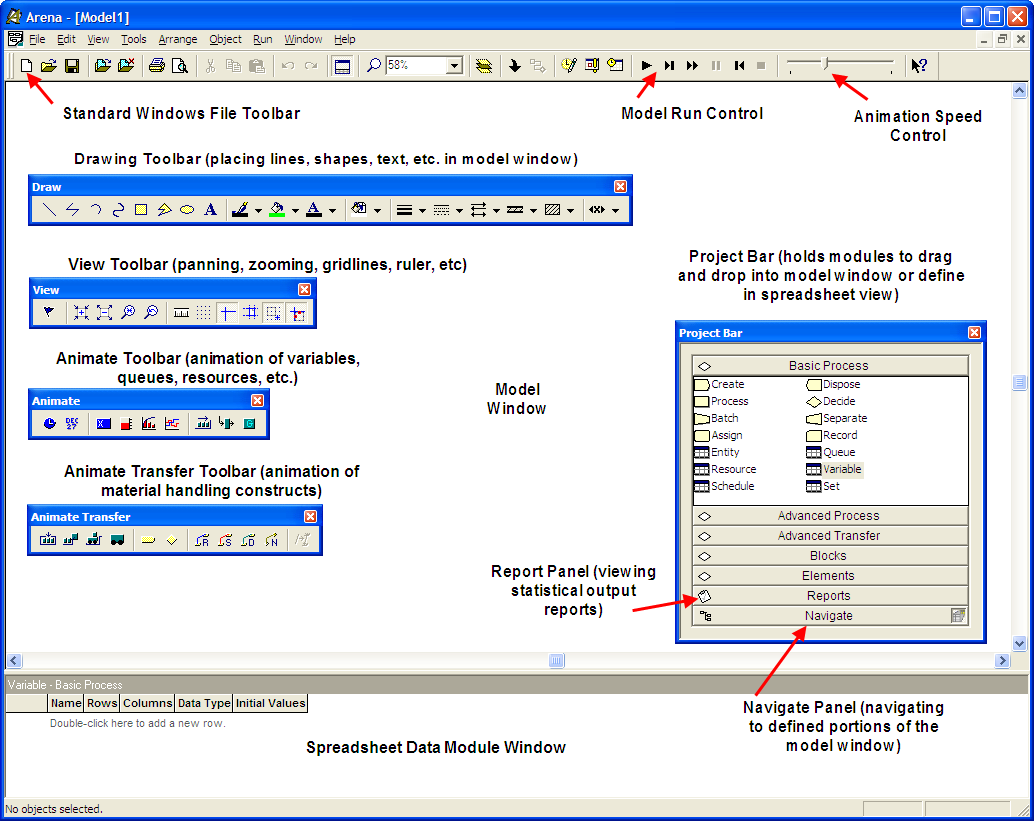
\includegraphics[width=0.8\linewidth,height=0.8\textheight]{./figures2/ch2/fig1ArenaEnvironment} 

}

\caption{The Arena Environment}\label{fig:ArenaEnvironment}
\end{figure}

\begin{figure}

{\centering 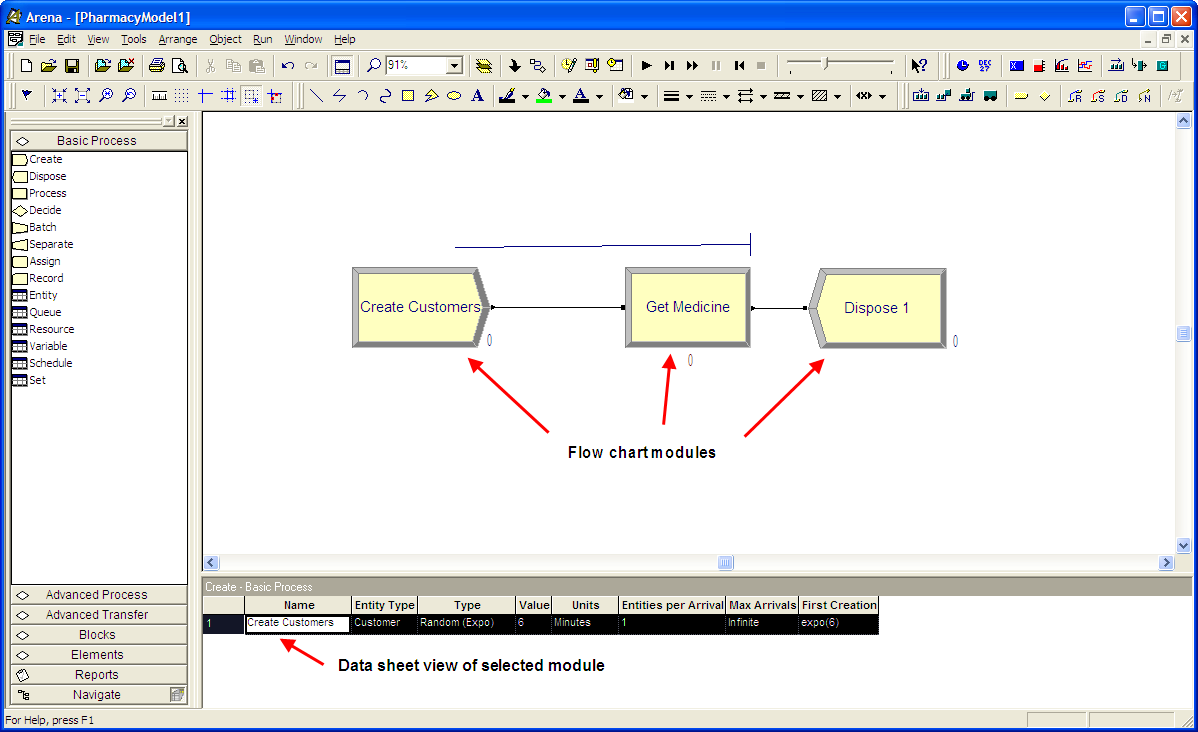
\includegraphics[width=0.8\linewidth,height=0.8\textheight]{./figures2/ch2/fig2ArenaToolbarsDocked} 

}

\caption{Arena environment with toolbars docked}\label{fig:ArenaToolbarsDocked}
\end{figure}

\hypertarget{MCinArena}{%
\section{Performing Simple Monte-Carlo Simulations using Arena}\label{MCinArena}}

The term Monte Carlo generally refers to the set of methods and
techniques predicated on estimating quantities by repeatedly sampling
from models/equations represented in a computer. As such, this
terminology is somewhat synonymous with computer simulation itself. The
term Monte Carlo gets its origin from the Monte Carlo casino in the
Principality of Monaco, where gambling and games of chance are well
known. There is no one Monte Carlo method. Rather there is a collection
of algorithms and techniques. In fact, the ideas of random number
generation and random variate generation previously discussed form the
foundation of Monte Carlo methods.

For the purposes of this chapter, we limit the term Monte Carlo methods
to those techniques for generating and estimating the expected values of
random variables, especially in regards to static simulation. In static
simulation, the notion of time is relatively straightforward with
respect to system dynamics. For a static simulation, time `ticks' in a
regular pattern and at each `tick' the state of the system changes (new
observations are produced). This should be contrasted with dynamic
simulation, where the state of the system evolves over time and the
state changes at irregularly (randomly occurring) points in time.
Dynamic simulation (specifically discrete-event simulation) will be the
subject of subsequent sections of this chapter and other chapters in the book.

\hypertarget{ssMC}{%
\subsection{Simple Monte Carlo Integration}\label{ssMC}}

In this section, we will illustrate one of the fundamental uses of Monte Carlo
methods: estimating the area of a function. Suppose we have some
function, \(g(x)\), defined over the range \(a \leq x \leq b\) and we want
to evaluate the integral:

\[\theta = \int\limits_{a}^{b} g(x)\mathrm{d}x\]

Monte Carlo methods allow us to evaluate this integral by couching the
problem as an estimation problem. It turns out that the problem can be
translated into estimating the expected value of a well-chosen random
variable. While a number of different choices for the random variable
exist, we will pick one of the simplest for illustrative purposes.
Define \(Y\) as follows with \(X \sim U(a,b)\):

\begin{equation}
Y = \left(b-a\right)g(X) 
\label{eq:Y}
\end{equation}

Notice that \(Y\) is defined in terms of \(g(X)\), which is also a random
variable. Because a function of a random variable is also a random
variable, this makes \(Y\) a random variable. Thus, the expectation of
\(Y\) can be computed as follows:

\begin{equation}
E[Y] = E[\left(b-a\right)g(X)] = \left(b-a\right)E[g(X)]
\label{eq:mcEY}
\end{equation}

Now, let us derive, \(E[g(X)]\). By definition,

\[E_{X}[g(X)] = \int\limits_{a}^{b} g(x)f_{X}(x)\mathrm{d}x\]

And, the probability density function for a \(X \sim U(a,b)\) random
variable is:

\[f_{X}(x) =
\begin{cases}
\frac{1}{b-a} & a \leq x \leq b\\
0   & \text{otherwise}
\end{cases}\]

Therefore,

\[E_{X}[g(X)] = \int\limits_{a}^{b} g(x)f_{X}(x)\mathrm{d}x = \int\limits_{a}^{b} g(x)\frac{1}{b-a}\mathrm{d}x\]

Substituting this result into Equation \eqref{eq:mcEY}, yields,

\begin{equation}
\begin{aligned}
E[Y] & = E[\left(b-a\right)g(X)] = \left(b-a\right)E_{X}[g(X)]\\
      & =  \left(b-a\right)\int\limits_{a}^{b} g(x)\frac{1}{b-a}\mathrm{d}x \\
      & = \int\limits_{a}^{b} g(x)\mathrm{d}x= \theta
\end{aligned}
\label{eq:mcEY2}
\end{equation}

Therefore, by estimating the expected value of \(Y\), we can estimate the
desired integral. From basic statistics, we know that a good estimator
for \(E[Y]\) is the sample average of observations of \(Y\). Let \((Y_1, Y_2,\ldots, Y_n)\) be a
random sample of observations of \(Y\). Let \(X_{i}\) be the \(i^{th}\)
observation of the variable \(X\). Substituting each \(X_{i}\) into Equation \eqref{eq:Y}
yields the \(i^{th}\) observation of \(Y\),

\begin{equation}
Y_{i} = \left(b-a\right)g(X_{i})
\label{eq:Yi}
\end{equation}

Then, the sample average of is:

\[\begin{aligned}
\bar{Y}(n) & = \frac{1}{n}\sum\limits_{i=1}^{n} Y_i = \left(b-a\right)\frac{1}{n}\sum\limits_{i=1}^{n}\left(b-a\right)g(X_{i})\\
  & = \left(b-a\right)\frac{1}{n}\sum\limits_{i=1}^{n}g(X_{i})\\\end{aligned}\]

where \(X_{i} \sim U(a,b)\). Thus, by simply generating
\(X_{i} \sim U(a,b)\), plugging the \(X_{i}\) into the function of interest,
\(g(x)\), taking the average over the values and multiplying by
\(\left(b-a\right)\), we can estimate the integral. This works for any
integral and it works for multi-dimensional integrals. While this
discussion is based on a single valued function, the theory scales to
multi-dimensional integration through the use of multi-variate
distributions. Now, let's illustrate the estimation of the area under a
curve for a simple function.

\begin{center}\rule{0.5\linewidth}{0.5pt}\end{center}

\begin{example}
\protect\hypertarget{exm:exMC}{}{\label{exm:exMC} }Suppose that we want to estimate
the area under \(f(x) = x^{\frac{1}{2}}\) over the range from \(1\) to \(4\)
as illustrated in Figure~\ref{fig:areaEst}. That is, we want to evaluate the integral:

\[\theta = \int\limits_{1}^{4} x^{\frac{1}{2}}\mathrm{d}x = \dfrac{14}{3}=4.6\bar{6}\]
\end{example}

\begin{center}\rule{0.5\linewidth}{0.5pt}\end{center}

\begin{figure}

{\centering 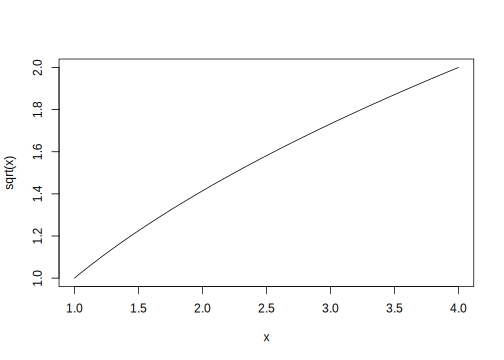
\includegraphics[width=0.7\linewidth]{02-Chapter2_files/figure-latex/areaEst-1} 

}

\caption{f(x) over the range from 1 to 4 }\label{fig:areaEst}
\end{figure}

According to the previously presented theory, we need to generate
\(X_i \sim U(1,4)\) and then compute \(\bar{Y}\), where
\(Y_i = (4-1)\sqrt{X{_i}}= 3\sqrt{X{_i}}\). This can be readily
accomplished using Arena. In addition, for this simple example,
we can easily check if our Monte Carlo approach is working because we
know the true area.

Example \ref{exm:exMC} estimates the area under a very simple function. In
fact, we know from basic calculus that the area is
\(\theta = 14/3 = 4.6\bar{6}\). As will be seen in the following solution. the result of the simulation is very close to the true value. The
difference between the estimated result and the true value is due to
\emph{sampling error}. We will discuss more about this important topic in Section \ref{ch3StatReview}.

Even though this example is rather simple, the basic idea can be used
for any complicated function and can be readily adapted for
multi-dimensional integrals. Now, let's solve this problem using Arena.

\hypertarget{ch2:staticArena}{%
\subsection{Arena Modules Needed for Static Simulation Examples}\label{ch2:staticArena}}

In this section we will implement the Monte Carlo area estimation problem using Arena. First, we need to introduce four programming modules that we will use to
develop these simulations.

\begin{itemize}
\item
  CREATE - This module creates entities that go through other modules
  causing their logic to be executed.
\item
  ASSIGN - This module allows us to assign values to variables with a
  model.
\item
  RECORD - This module permits the collection of statistics on
  expressions.
\item
  DISPOSE - This module disposes of entities after they are done
  executing within the model.
\item
  VARIABLE - This module is used to define variables within the model
  and to initialize their values.
\end{itemize}

These modules (VARIABLE, CREATE, ASSIGN, RECORD, and DISPOSE) all have
additional functionality that will be described later in the text;
however, the above definitions will suffice to get us started for this
example.

Second, we need to have a basic understanding of the mathematical and
distribution function modeling that is available within Arena. While Arena has a
wide range of mathematical and distribution modeling capabilities, only
the subset necessary for the Monte Carlo examples will be
illustrated in this section.

Here is a overview of the mathematical and distribution functions that
we will be using:

\begin{itemize}
\tightlist
\item
  UNIF(a,b) - This function will return a random variate from a
  uniform distribution over the range from a to b.
\end{itemize}

\begin{itemize}
\item
  DISC(\(cp_1\), \(v_1\), \(cp_2\), \(v_2\), ...) - This function returns a
  random variate from a discrete empirical cumulative distribution
  function, where \(cp_i\), \(v_i\) are the the pairs
  \(cp_i = P\left\{X \leq v_i\right\}\) for the CDF.
\item
  SQRT(x) - This function returns the square root of x.
\item
  MN(x1, x2,...) - This function returns the minimum of the values
  presented.
\item
  MX(x1, x2,...) - This function returns the maximum of the values
  presented.
\end{itemize}

In the following sections, we will put these modules and functions into practice.

\hypertarget{ch2:areaArena}{%
\subsection{Area Estimation via Arena}\label{ch2:areaArena}}

In the example, we are interested in estimating
the area under \(f(x) = x^{\frac{1}{2}}\) over the range from \(1\) to \(4\).
The following pseudo-code outlines the basic code that will be used for estimating
the area of the function within Arena.

\begin{verbatim}
CREATE 1 entity
BEGIN ASSIGN
  vXi = UNIF(1,4) 
  vFx = SQRT(vXi) 
  vY = (4.0 - 1.0)*vFx
END ASSIGN
RECORD vY 
DISPOSE
\end{verbatim}

This pseudo-code is very self-explanatory. It outlines the modeling approach using syntax that is similar to constructs that appear in Arena. We will define more carefully the use of pseudo-code in the modeling process starting in Chapter \ref{ch3}. The CREATE statement generates 1 entity, which then executes the rest of the code. We will learn more about the concept of an entity when we use entities in the DEDS modeling in later sections of the book. For the purposes of this example, think of the entity as representing an
observation that will invoke the subsequent listed commands. The ASSIGN
represents the assignments that generate the value of \(x\), evaluate
\(f(x)\), and compute \(y\). The RECORD indicates that statistics should be
collected on the value of \(y\). Finally, the DISPOSE indicates that the
generated entity should be disposed (removed from the program). This is
only pseudo-code! It does not represent a functioning Arena model. However, it
is useful to conceptualize the program in this fashion so that you can
more readily implement it within the Arena environment.

\begin{figure}

{\centering 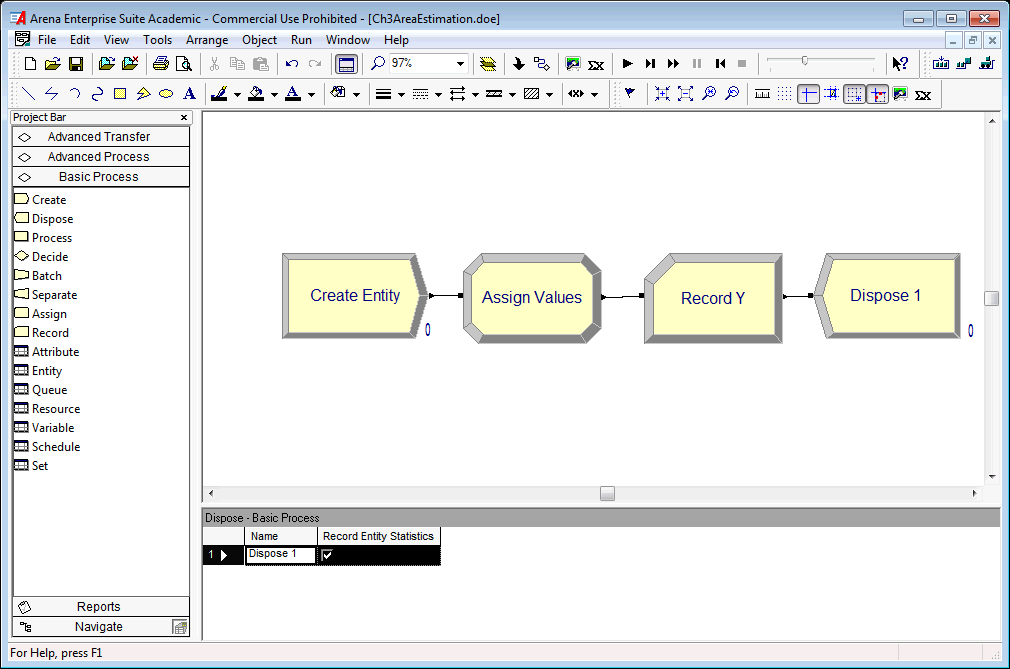
\includegraphics[width=0.8\linewidth,height=0.8\textheight]{./figures2/ch2/fig3AreaEstArena} 

}

\caption{Arena model for estimating the area of f(x)= sqrt(x)}\label{fig:AreaEstArena}
\end{figure}

Figure~\ref{fig:AreaEstArena} represent the flow chart solution
within the environment. Notice the CREATE, ASSIGN, RECORD, and DISPOSE
modules laid out in the model window. A CREATE module creates entities
that flow through other modules. Figure \ref{fig:AreaEstCreate} illustrates the creating of 1 entity by setting the maximum number of entities field to the value 1. Since the First Creation field has a value of 0.0, there will be 1 entity that
is created at time 0. The CREATE module will be discussed in further
detail, later in this chapter. The created entity will move to the next
module (ASSIGN) and cause its logic to be executed.

\begin{figure}

{\centering 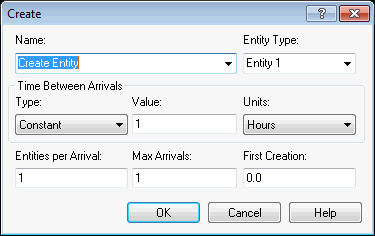
\includegraphics[width=0.6\linewidth,height=0.6\textheight]{./figures2/ch2/fig4AreaEstCreate} 

}

\caption{Creating 1 entity with a CREATE module}\label{fig:AreaEstCreate}
\end{figure}

An ASSIGN module permits the assignment of values to various quantities
of interest in the model. In
Figure~\ref{fig:AreaEstAssign}, a listing of the assignments for
generating the value of \(x\), computing \(f(x)\), and \(y\) are provided.
Each assignment is executed in the order listed. It is important to get
the order correct when you write your programs!

\begin{figure}

{\centering 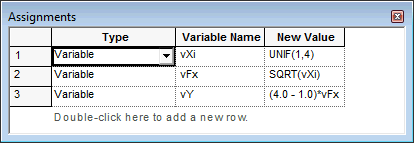
\includegraphics[width=0.6\linewidth,height=0.6\textheight]{./figures2/ch2/fig5AreaEstAssign} 

}

\caption{Making assignments using an ASSIGN module}\label{fig:AreaEstAssign}
\end{figure}

Figure~\ref{fig:AreaEstRecord} shows the RECORD module for this
situation. The value of the variable \(vY\) is in the Value text field.
Because the Type of the record is set at Expression, the value of this
variable will be observed every time an entity passes through the
module. The observations will be tabulated so that the sample average
and 95\% half-width will be reported automatically on the output reports,
labeled by the text in the Tally Name field. The results are illustrated
in Figure~\ref{fig:AreaEstResults}.

\begin{figure}

{\centering 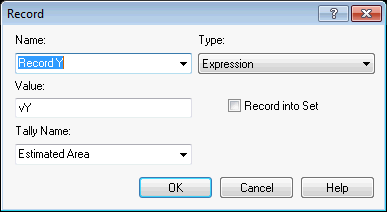
\includegraphics[width=0.6\linewidth,height=0.6\textheight]{./figures2/ch2/fig6AreaEstRecord} 

}

\caption{Recording statistics on an expression using a RECORD module}\label{fig:AreaEstRecord}
\end{figure}

\begin{figure}

{\centering 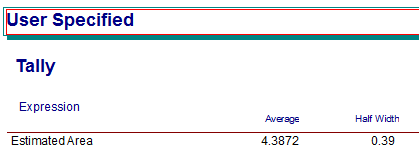
\includegraphics[width=0.6\linewidth,height=0.6\textheight]{./figures2/ch2/fig7AreaEstResults} 

}

\caption{Results from the area estimation model}\label{fig:AreaEstResults}
\end{figure}

In order to run the model, you must indicate the required number of
observations. Since each run of the model produces 1 entity and thus 1
observation, you need to specify the number of times that you want to
run the model. This is accomplished using the Run Setup menu item.
Figure~\ref{fig:AreaEstRunSetup} shows that the model is set to run
for 20 replications. Replications will be discussed later in the text, but
for now, you can think of a replication as a running of the model to
produce observations. Each replication is independent of other
replications. Thus, the observations across replications form a random
sample of the observations. Arena will automatically report the statistics across the
replications.

\begin{figure}

{\centering 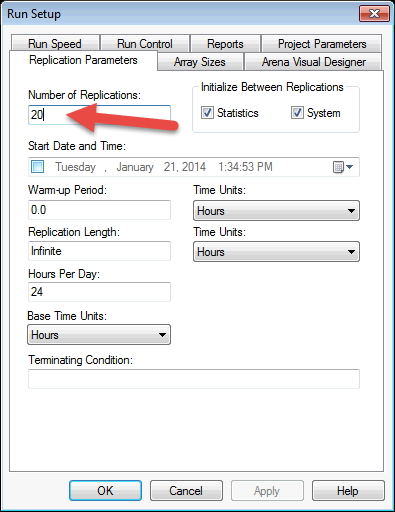
\includegraphics[width=0.55\linewidth,height=0.55\textheight]{./figures2/ch2/fig8AreaEstRunSetup} 

}

\caption{Setting up the simulation to replicate 20 observations}\label{fig:AreaEstRunSetup}
\end{figure}

Figure~\ref{fig:AreaEstResults} shows the results of estimating the
area of the curve. Notice that the average value (4.3872) reported for
the variable observed in the RECORD module is close to the true value of
\(4.6\bar{6}\) computed for Example \ref{exm:exMC}. The difference between the estimated value and the true value is due to sampling error. We will discuss how to control sampling error within Chapter \ref{ch3}. The area estimation model can be found within this Chapter's files as \emph{AreaEstimation.doe}.

Now let's look at a slightly more complex static simulation.

\FloatBarrier

\hypertarget{the-news-vendor-problem}{%
\subsection{The News Vendor Problem}\label{the-news-vendor-problem}}

The news vendor model is a classic inventory model that allows for the
modeling of how much to order for a decision maker facing uncertain
demand for an upcoming period of time. It takes on the news vendor
moniker because of the context of selling newspapers at a newsstand. The
vendor must anticipate how many papers to have on hand at the beginning
of a day so as to not run short or have papers left over. This idea can
be generalized to other more interesting situations (e.g.~air plane
seats). Discussion of the news vendor model is often presented in
elementary textbooks on inventory theory. The reader is referred to
\citep{Muckstadt2010aa} for a discussion of this model.

The basic model is considered a single period model; however, it can be
extended to consider an analysis covering multiple (or infinite) future
periods of demand. The representation of the costs within the modeling
offers a number of variations.

Let \(D\) be a random variable representing the demand for the period. Let
\(F(d)= P[D \leq d]\) be the cumulative distribution function for the
demand. Define \(G(q,D)\) as the profit at the end of the period when \(q\)
units are ordered at the start of the period with \(D\) units of demand.
The parameter \(q\) is the decision variable associated with this model.
Depending on the value of \(q\) chosen by the news vendor, a profit or
loss will occur.

There are two cases to consider \(D \geq q\) or \(D < q\). That is, when
demand is greater than or equal to the amount ordered at the start of
the period and when demand is less than the amount ordered at the start
of the period. If \(D \geq q\) the news vendor runs out of items, and if
\(D < q\) the news vendor will have items left over.

In order to develop a profit model for this situation, we need to define
some model parameters. In addition, we need to determine the amount that
we might be short and the amount we might have left over in order to
determine the revenue or loss associated with a choice of \(q\). Let \(c\)
be the purchase cost. This is the cost that the news vendor pays the
supplier for the item. Let \(s\) be the selling price. This is the amount
that the news vendor charges customers. Let \(u\) be the salvage value
(i.e.~the amount per unit that can be received for the item after the
planning period). For example, the salvage value can be the amount that
the news vendor gets when selling a left over paper to a recycling
center. We assume that selling price \(>\) purchase cost \(>\) salvage
value.

Consider the context of a news vendor planning for the day. What is the
possible amount sold? If \(D\) is the demand for the day and we start with
\(q\) items, then the most that can be sold is \(\min(D, q)\). That is, if
\(D\) is bigger than \(q\), you can only sell \(q\). If \(D\) is smaller than
\(q\), you can only sell \(D\).

What is the possible amount left over (available for salvage)? If \(D\) is
the demand and we start with \(q\), then there are two cases: 1) demand is
less than the amount ordered (\(D < q\)) or 2) demand is greater than or
equal to the amount ordered (\(D \geq q\)). In case 1, we will have \(q-D\)
items left over. In case 2, we will have \(0\) left over. Thus, the amount
left over at the end of the day is \(\max(0, q-D)\). Since the news vendor
buys \(q\) items for \(c\), the cost of the items for the day is
\(c \times q\). Thus, the profit has the following form:

\begin{equation}
G(D,q) = s \times \min(D, q) + u \times \max(0, q-D) - c \times q
\label{eq:ExpRev}
\end{equation}

In words, the profit is equal to the sales revenue plus the salvage
revenue minus the ordering cost. The sales revenue is the selling price
times the amount sold. The salvage revenue is the salvage value times
the amount left over. The ordering cost is the cost of the items times
the amount ordered. To find the optimal value of \(q\), we should try to
maximize the expected profit. Since \(D\) is a random variable, \(G(D,q)\)
is also a random variable. Taking the expected value of both sides of
Equation~\eqref{eq:ExpRev}, yields:

\[g(q) = E[G(D,q)] =  sE[\min(D, q)] + uE[\max(0, q-D)] - cq\]

Whether or not this equation can be optimized depends on the form of the
distribution of \(D\); however, simulation can be used to estimate this
expected value for any given \(q\). Let's look at an example.

\begin{center}\rule{0.5\linewidth}{0.5pt}\end{center}

\begin{example}
\protect\hypertarget{exm:BBQWing}{}{\label{exm:BBQWing} }Sly's convenience store sells BBQ wings for 25 cents a piece. They cost 15
cents a piece to make. The BBQ wings that are not sold on a given day
are purchased by a local food pantry for 2 cents each. Assuming that Sly
decides to make 30 wings a day, what is the expected revenue for the
wings provided that the demand distribution is as show in
Table~\ref{tab:BBQWingDemand}.
\end{example}

\begin{center}\rule{0.5\linewidth}{0.5pt}\end{center}

\hypertarget{tab:BBQWingDemand}{}
\begin{longtable}[]{@{}cccccccc@{}}
\caption{\label{tab:BBQWingDemand} Distribution of BBQ wing demand}\tabularnewline
\toprule
\(d_{i}\) & 5 & 10 & 40 & 45 & 50 & 55 & 60\tabularnewline
\midrule
\endfirsthead
\toprule
\(d_{i}\) & 5 & 10 & 40 & 45 & 50 & 55 & 60\tabularnewline
\midrule
\endhead
\(f(d_{i})\) & 0.1 & 0.2 & 0.3 & 0.2 & 0.1 & 0.05 & 0.05\tabularnewline
\(F(d_{i})\) & 0.1 & 0.3 & 0.6 & 0.8 & 0.9 & 0.95 & 1.0\tabularnewline
\bottomrule
\end{longtable}

The pseudo-code for the news vendor
problem will require the generation of the demand from BBQ Wing demand distribution. In order to generate from this distribution, the DISC() function should be used. Since the cumulative distribution has already been computed, it
is straight forward to write the inputs for the DISC() function. The
function specification is:

\[\textit{DISC}(0.1,5,0.3,10,0.6,40,0.8,45,0.9,50,0.95,55,1.0,60)\]

Notice the pairs (\(F(d_{i})\), \(d_{i}\)). The final value of \(F(d_{i})\)
must be the value 1.0.

First, let us define some variables to be used in the modeling: demand,
amount sold, amount left at the end of the day, sales revenue, salvage
revenue, price per unit, cost per unit, salvage per unit, and order
quantity.

\begin{itemize}
\item
  Let vDemand represent the daily demand
\item
  Let vAmtSold represent the amount sold
\item
  Let vAmtLeft represent the amount left at the end of the day
\item
  Let vSalesRevenue represent the sales revenue
\item
  Let vSalvageRevenue represent the salvage revenue
\item
  Let vPricePerUnit = 0.25 represent the price per unit
\item
  Let vCostPerUnit = 0.15 represent the cost per unit
\item
  Let vSalvagePerUnit = 0.02 represent the salvage value per unit
\item
  Let vOrderQty = 30 represent the amount ordered each day
\end{itemize}

The pseudo-code for this situation is as follows.

\begin{verbatim}
CREATE 1 entity
BEGIN ASSIGN
  vDemand = DISC(0.1,5,0.3,10,0.6,40,0.8,45,0.9,50,0.95,55,1.0,60) 
  vAmtSold = MN(vDemand, vOrderQty) 
  vAmtLeft = MX(0, vOrderQty - vDemand)
  vSalesRevenue = vAmtSold*vPricePerUnit 
  vSalvageRevenue = vAmtLeft*vSalvagePerUnit 
  vOrderingCost = vCostPerUnit*vOrderQty
  vProfit = vSalesRevenue + vSalvageRevenue - vOrderingCost
END ASSIGN
RECORD vProfit
DISPOSE
\end{verbatim}

The CREATE module creates the an entity to
represent the day. The ASSIGN modules implement the logic associated
with the news vendor problem. The MN() function is used to compute the
minimum of the demand and the amount ordered. The MX() function
determines the amount unsold. The DISC() function implements the CDF of
the demand in order to generate the daily demand. The rest of the
equations follow directly from the previous discussion. The flow
chart solution is illustrated in Figure \ref{fig:NewsVendorArena} and uses the same flow chart modules (CREATE, ASSIGN, RECORD, DISPOSE) as in the last example.

\begin{figure}

{\centering 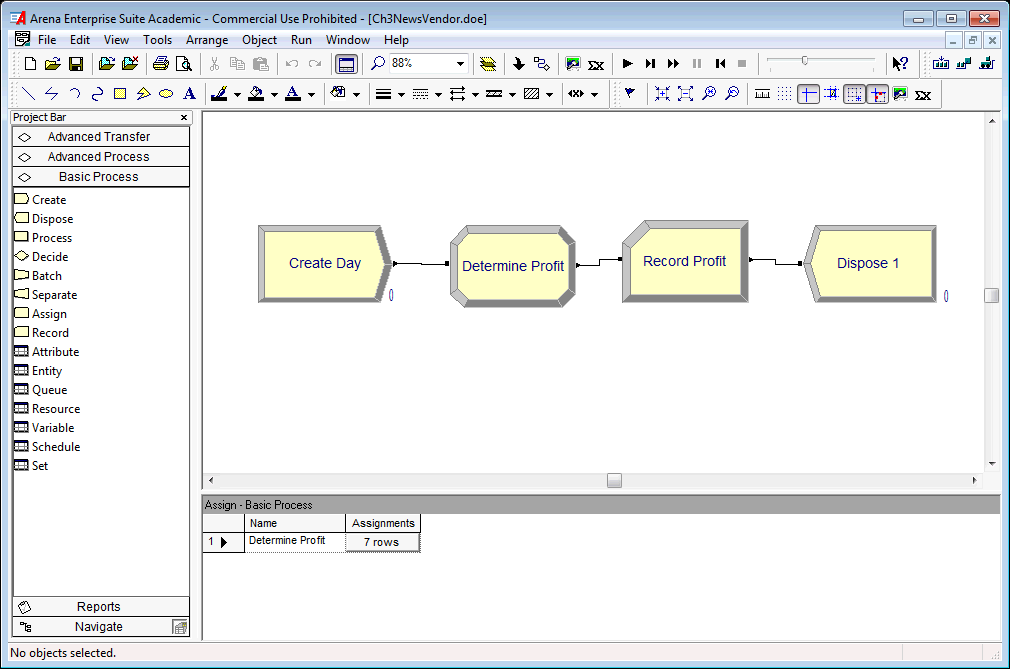
\includegraphics{./figures2/ch2/fig9NewsVendorArena} 

}

\caption{Model for news vendor problem}\label{fig:NewsVendorArena}
\end{figure}

To implement the variable definitions from the pseudo-code, you need to
use a VARIABLE module to provide the initial values of the variables.
Notice in Figure~\ref{fig:VendorVariables} the definition of each variable
and how the initial value of the variable \emph{vCostPerUnit} is showing. The
CREATE module is setup exactly as in the last example. The created
entity will move to the next module (ASSIGN) illustrated in
Figure~\ref{fig:NewsVendorAssignments}. The assignments follow
exactly the previously illustrate pseudo-code. Running the model for 100
days results in the output illustrated in Figure~\ref{fig:NewsVendorResults}.

\begin{figure}

{\centering 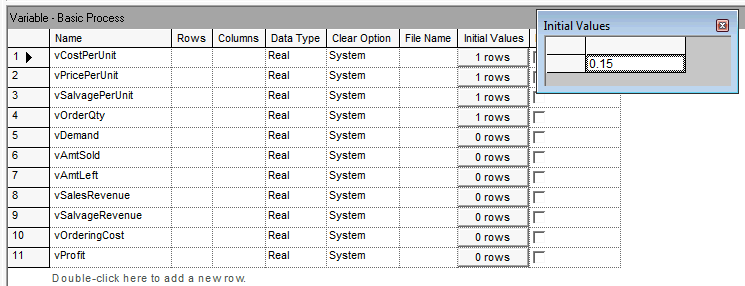
\includegraphics{./figures2/ch2/fig10NewsVendorVariables} 

}

\caption{Variable definitions used in the news vendor solution}\label{fig:VendorVariables}
\end{figure}

\begin{figure}

{\centering 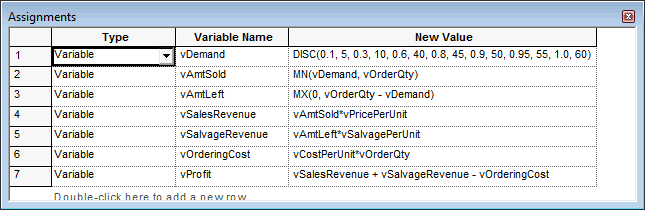
\includegraphics{./figures2/ch2/fig11NewsVendorAssignments} 

}

\caption{Assignments used in the news vendor solution}\label{fig:NewsVendorAssignments}
\end{figure}

\begin{figure}

{\centering 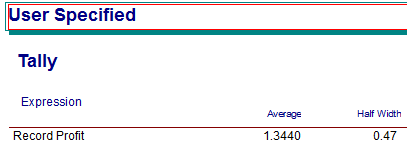
\includegraphics{./figures2/ch2/fig12NewsVendorResults} 

}

\caption{Results based on 100 replications of the news vendor model}\label{fig:NewsVendorResults}
\end{figure}

The news vendor model can be found within this Chapter's files as \emph{NewsVendor.doe}.

In this section, we explored how to develop models in for which time is
not a significant factor. In the case of the news vendor problem, where
we simulated each day's demand, time advanced at regular intervals. In
the case of the area estimation problem, time was not a factor in the simulation.
These types of simulations are often termed static simulation. In the
next section, we begin our exploration of simulation where time is an
integral component in driving the behavior of the system. In addition,
we will see that time will not necessarily advance at regular intervals
(e.g.~hour 1, hour 2, etc.). This will be the focus of the rest of the
book.

\hypertarget{HowDEDSClockWorks}{%
\section{How the Discrete-Event Clock Works}\label{HowDEDSClockWorks}}

This section introduces the concept of how time evolves in a discrete
event simulation. This topic will also be revisited in future chapters
after you have developed a deeper understanding for many of the
underlying elements of simulation modeling.

In discrete-event dynamic systems, an event is something that happens at
an instant in time which corresponds to a change in system state. An
event can be conceptualized as a transmission of information that causes
an action resulting in a change in system state. Let's consider a simple
bank which has two tellers that serve customers from a single waiting
line. In this situation, the system of interest is the bank tellers
(whether they are idle or busy) and any customers waiting in the line.
Assume that the bank opens at 9 am, which can be used to designate time
zero for the simulation. It should be clear that if the bank does not
have any customers arrive during the day that the state of the bank will
not change. In addition, when a customer arrives, the number of
customers in the bank will increase by one. In other words, an arrival
of a customer will change the state of the bank. Thus, the arrival of a
customer can be considered an event.

\begin{figure}

{\centering 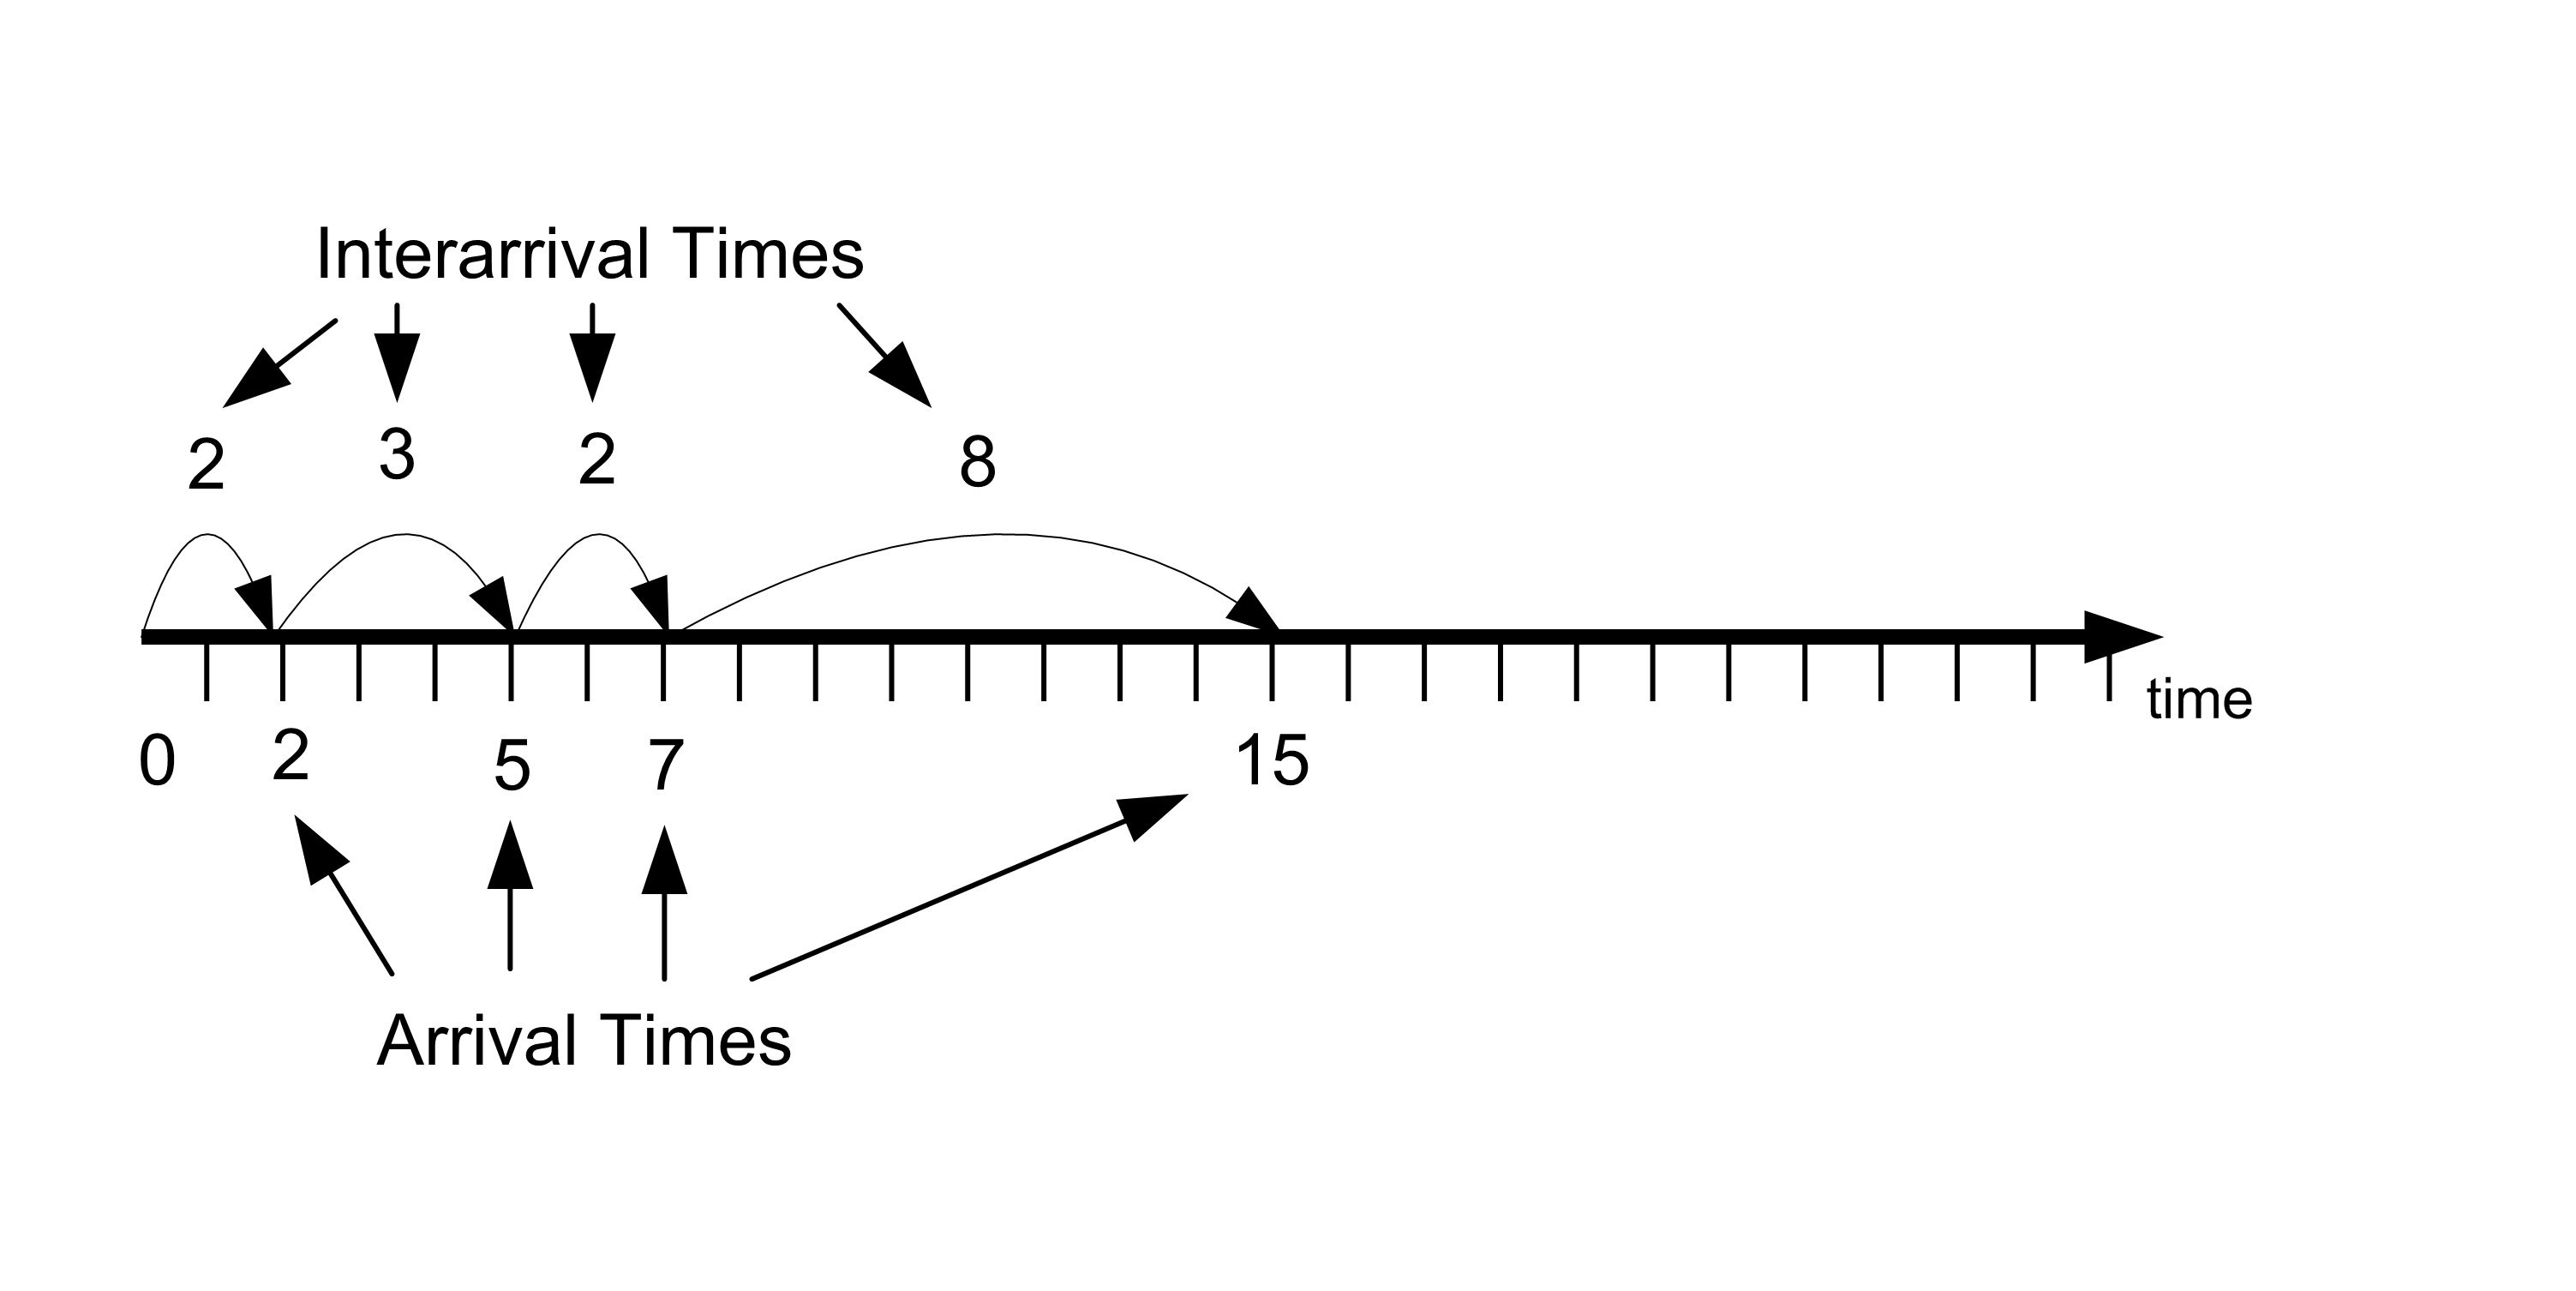
\includegraphics{./figures2/ch2/fig13ArrivalProcess} 

}

\caption{Customer arrival process}\label{fig:ArrivalProcess}
\end{figure}

\hypertarget{tab:CustArrivals}{}
\begin{longtable}[]{@{}ccc@{}}
\caption{\label{tab:CustArrivals} Customer time of arrivals}\tabularnewline
\toprule
Customer & Time of arrival & Time between arrival\tabularnewline
\midrule
\endfirsthead
\toprule
Customer & Time of arrival & Time between arrival\tabularnewline
\midrule
\endhead
1 & 2 & 2\tabularnewline
2 & 5 & 3\tabularnewline
3 & 7 & 2\tabularnewline
4 & 15 & 8\tabularnewline
\bottomrule
\end{longtable}

Figure~\ref{fig:ArrivalProcess} illustrates a time line of customer
arrival events. The values for the arrival times in Table \ref{tab:CustArrivals} have been rounded to
whole numbers, but in general the arrival times can be any real valued
numbers greater than zero. According to the figure, the first customer
arrives at time two and there is an elapse of three minutes before
customer 2 arrives at time five. From the discrete-event perspective,
\emph{nothing} is happening in the bank from time \([0,2)\); however, at time 2, an
arrival event occurs and the subsequent actions associated with this
event need to be accounted for with respect to the state of the system. An event denotes an instance of time that changes the state of the system. Since an event causes actions that result in a change of system state,
it is natural to ask: What are the actions that occur when a customer arrives to the
bank?

\begin{itemize}
\item
  The customer enters the waiting line.
\item
  If there is an available teller, the customer will immediately exit
  the line and the available teller will begin to provide service.
\item
  If there are no tellers available, the customer will remain waiting
  in the line until a teller becomes available.
\end{itemize}

Now, consider the arrival of the first customer. Since the bank opens at
9 am with no customer and all the tellers idle, the first customer will
enter and immediately exit the queue at time 9:02 am (or time 2) and
then begin service. After the customer completes service, the customer
will exit the bank. When a customer completes service (and departs the
bank) the number of customers in the bank will decrease by one. It
should be clear that some actions need to occur when a customer
completes service. These actions correspond to the second event
associated with this system: the customer service completion event. What
are the actions that occur at this event?

\begin{itemize}
\item
  The customer departs the bank.
\item
  If there are waiting customers, the teller indicates to the next
  customer that he/she will serve the customer. The customer will exit
  the waiting line and will begin service with the teller.
\item
  If there are no waiting customers, then the teller will become idle.
\end{itemize}

Figure~\ref{fig:ServiceProcess} contains the service times for each
of the four customers that arrived in
Figure~\ref{fig:ArrivalProcess}. Examine the figure with respect to
customer 1. Based on the figure, customer 1 can enter service at time
two because there were no other customers present in the bank. Suppose
that it is now 9:02 am (time 2) and that the service time of customer 1
is known \emph{in advance} to be 8 minutes as indicated in Table \ref{tab:CustServiceTimes}. From this information, the time that customer 1 is going to complete service can be pre-computed. From
the information in the figure, customer 1 will complete service at time
10 (current time + service time = 2 + 8 = 10). Thus, it should be
apparent, that for you to recreate the bank's behavior over a time
period that you must have knowledge of the customer's service times. The
service time of each customer coupled with the knowledge of when the
customer began service allows the time that the customer will complete
service and depart the bank to be computed in advance. A careful
inspection of Figure~\ref{fig:ServiceProcess} and knowledge of how banks operate
should indicate that a customer will begin service either immediately
upon arrival (when a teller is available) or coinciding with when
another customer departs the bank after being served. This latter
situation occurs when the queue is not empty after a customer completes
service. The times that service completions occur and the times that
arrivals occur constitute the pertinent events for simulating this
banking system.

\begin{figure}

{\centering 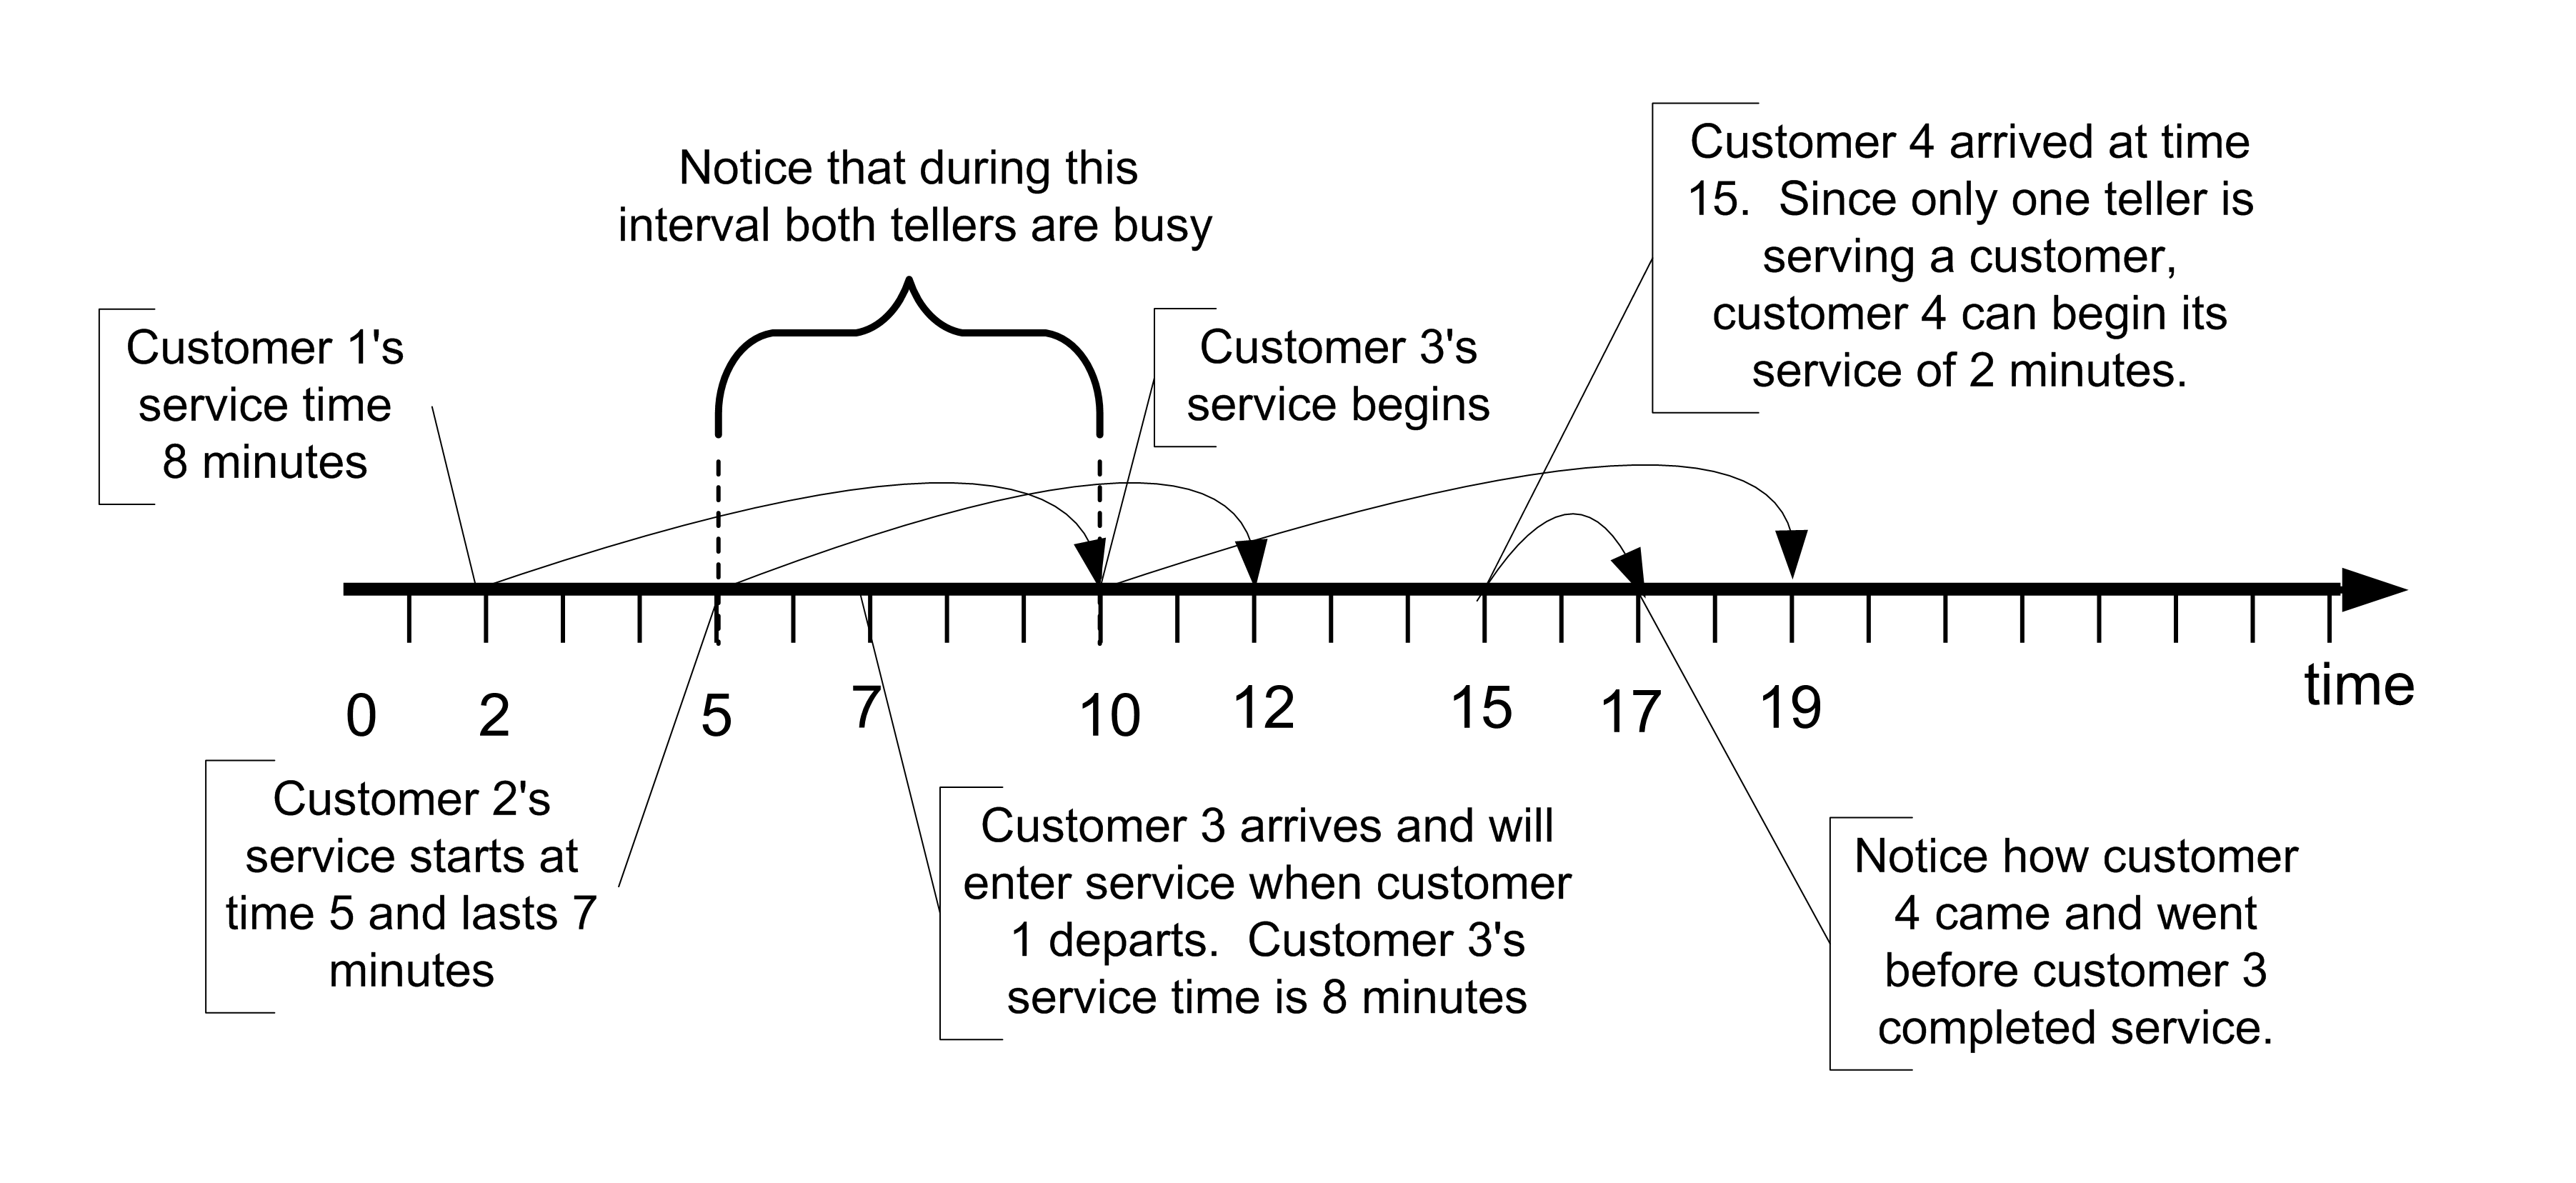
\includegraphics{./figures2/ch2/fig14ServiceProcess} 

}

\caption{Customer service process}\label{fig:ServiceProcess}
\end{figure}

\hypertarget{tab:CustServiceTimes}{}
\begin{longtable}[]{@{}cccc@{}}
\caption{\label{tab:CustServiceTimes} Service time for first four customers}\tabularnewline
\toprule
Customer & Service Time Started & Service Time & Service Time Completed\tabularnewline
\midrule
\endfirsthead
\toprule
Customer & Service Time Started & Service Time & Service Time Completed\tabularnewline
\midrule
\endhead
1 & 2 & 8 & 10\tabularnewline
2 & 5 & 7 & 12\tabularnewline
3 & 10 & 9 & 19\tabularnewline
4 & 15 & 2 & 17\tabularnewline
\bottomrule
\end{longtable}

If the arrival and the service completion events are combined, then the
time ordered sequence of events for the system can be determined.
Figure~\ref{fig:TimeOrderedProcess} illustrates the events ordered by time
from smallest event time to largest event time. Suppose you are standing
at time two. Looking forward, the next event to occur will be at time 5
when the second customer arrives. When you simulate a system, you must
be able to generate a sequence of events so that, at the occurrence of
each event, the appropriate actions are invoked that change the state of
the system.

\begin{figure}

{\centering 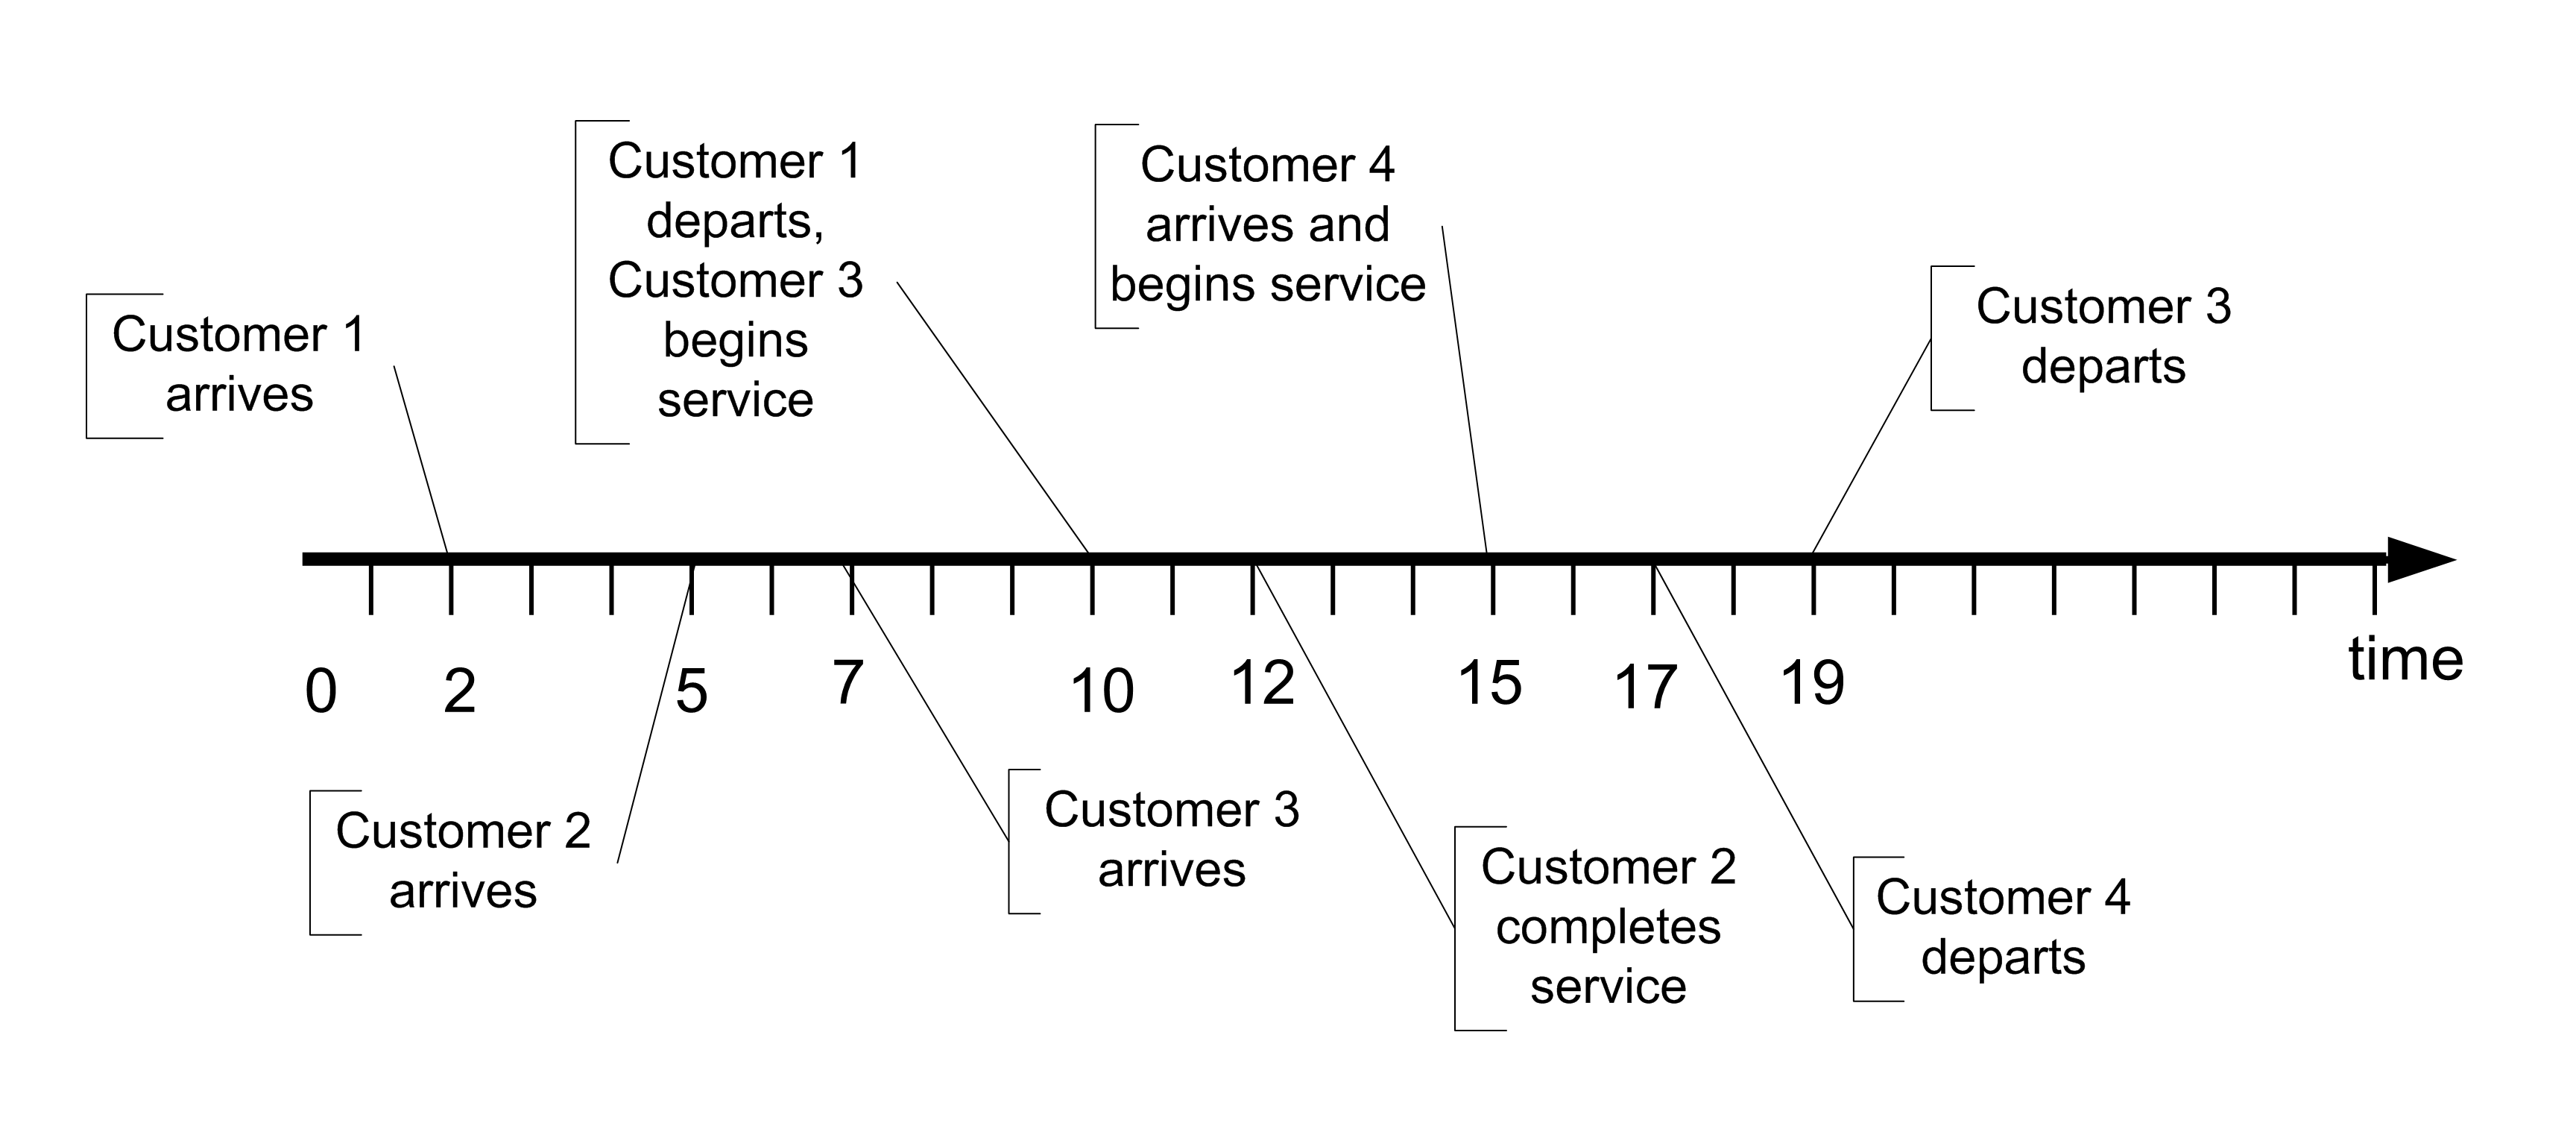
\includegraphics{./figures2/ch2/fig15TimeOrderedProcess} 

}

\caption{Events ordered by time}\label{fig:TimeOrderedProcess}
\end{figure}

In the following table, \(c_i\) represents the \(i^{th}\) customer and \(s_j\) represents the \(j^{th}\) teller.

\begin{longtable}[]{@{}ccl@{}}
\toprule
Time & Event & Comment\tabularnewline
\midrule
\endhead
0 & Bank 0pens &\tabularnewline
2 & Arrival & \(c_1\) arrives, enters service for 8 min., \(s_1\) becomes busy\tabularnewline
5 & Arrival & \(c_2\) arrives, enters service for 7 min., the \(s_2\) becomes busy\tabularnewline
7 & Arrival & \(c_3\) arrives, waits in queue\tabularnewline
10 & Service Completion & \(c_1\) completes service, \(c_3\) exits queue, enters service for 9 min.\tabularnewline
12 & Service Completion & \(c_2\) completes service, queue is empty, \(s_2\) becomes idle\tabularnewline
15 & Arrival & \(c_4\) arrives, enters service for 2 min., \(s_2\) becomes busy\tabularnewline
17 & Service Completion & \(c_4\) completes service, \(s_2\) becomes idle\tabularnewline
19 & Service Completion & \(c_3\) completes service, \(s_1\) becomes idle\tabularnewline
\bottomrule
\end{longtable}

\hfill\break

The real system will simply evolve over time; however, a simulation of
the system must recreate the events. In simulation, events are created
by adding additional logic to the normal state changing actions. This
additional logic is responsible for scheduling future events that are
implied by the actions of the current event. For example, when a
customer arrives, the time to the next arrival can be generated and
scheduled to occur at some future time. This can be done by generating
the time until the next arrival and adding it to the current time to
determine the actual arrival time. Thus, all the arrival times do not
need to be pre-computed prior to the start of the simulation. For
example, at time two, customer 1 arrived. Customer 2 arrives at time 5.
Thus, the time between arrivals (3 minutes) is added to the current time
and customer 2's arrival at time 5 is scheduled to occur. Every time an
arrival occurs this additional logic is invoked to ensure that more
arrivals will continue within the simulation.

Adding additional scheduling logic also occurs for service completion
events. For example, since customer 1 immediately enters service at time
2, the service completion of customer 1 can be scheduled to occur at
time 12 (current time + service time = 2 + 10 = 12). Notice that other
events may have already been scheduled for times less than time 12. In
addition, other events may be inserted before the service completion at
time 12 actually occurs. From this, you should begin to get a feeling
for how a computer program can implement some of these ideas.

Based on this intuitive notion for how a computer simulation may
execute, you should realize that computer logic processing need only
occur at the event times. That is, the state of the system does not
change between events. Thus, it is \emph{not necessary} to step incrementally
through time checking to see if something happens at time 0.1, 0.2, 0.3,
etc. (or whatever time scale you envision that is fine enough to not
miss any events). Thus, in a discrete-event dynamic system simulation the clock does not
``tick'' at regular intervals. Instead, the simulation clock jumps from
event time to event time. As the simulation moves from the current event
to the next event, the current simulation time is updated to the time of
the next event and any changes to the system associated with the next
event are executed. This allows the simulation to evolve over time.

\hypertarget{simulating-a-queueing-system-by-hand}{%
\section{Simulating a Queueing System By Hand}\label{simulating-a-queueing-system-by-hand}}

This section builds on the concepts discussed in the previous section in order to provide insights into how discrete event simulations operate. In order to do this, we will simulate a simple queueing system by hand. That is, we will process each of the events that occur as well as the state changes in order to trace the operation of the system through time.

Consider again the simple banking system described in the previous
section. To simplify the situation, we assume that there is only one
teller that is available to provide service to the arriving customers.
Customers that arrive while the teller is already helping a customer
form a single waiting line, which is handled in a first come, first
served manner. Let's assume that the bank opens at 9 am with no
customers present and the teller idle. The time of arrival of the first
eight customers is provided in the following Table \ref{tab:ArrServTime}

\hypertarget{tab:ArrServTime}{}
\begin{longtable}[]{@{}lll@{}}
\caption{\label{tab:ArrServTime} Time of arrivals and service times for 8 customers}\tabularnewline
\toprule
Customer Number & Time of Arrival & Service Time\tabularnewline
\midrule
\endfirsthead
\toprule
Customer Number & Time of Arrival & Service Time\tabularnewline
\midrule
\endhead
1 & 3 & 4\tabularnewline
2 & 11 & 4\tabularnewline
3 & 13 & 4\tabularnewline
4 & 14 & 3\tabularnewline
5 & 17 & 2\tabularnewline
6 & 19 & 4\tabularnewline
7 & 21 & 3\tabularnewline
8 & 27 & 2\tabularnewline
\bottomrule
\end{longtable}

We are going to process these customers in order to recreate the
behavior of this system over from time 0 to 31 minutes. To do this, we
need to be able to perform the ``bookkeeping'' that a computer simulation
model would normally perform for us. Thus, we will need to define some
variables associated with the system and some attributes associated with
the customers. Consider the following system variables.

System Variables

\begin{itemize}
\item
  Let \(t\) represent the current simulation clock time.
\item
  Let \(N(t)\) represent the number of customers in the system (bank) at
  any time \(t\).
\item
  Let \(Q(t)\) represent the number of customers waiting in line for the
  teller at any time \(t\).
\item
  Let \(B(t)\) represent whether or not the teller is busy (1) or
  idle (0) at any time \(t\).
\end{itemize}

Because we know the number of tellers available, we know that the
following relationship holds between the variables:

\[N\left( t \right) = Q\left( t \right) + B(t)\]

Note also that, knowledge of the value of \(N(t)\) is sufficient to
determine the values of \(Q(t)\) and \(B(t)\) at any time \(t.\) For example,
if we know that there are 3 customers in the bank, then
\(N\left( t \right) = 3\), and since the teller must be serving 1 of those
customers, \(B\left( t \right) = 1\) and there must be 2 customers
waiting, \(Q\left( t \right) = 2\). In this situation, since
\(N\left( t \right)\), is sufficient to determine all the other system
variables, we can say that \(N\left( t \right)\) is the system's \emph{state
variable}. The state variable(s) are the minimal set of system
variables that are necessary to represent the system's behavior over
time. We will keep track of the values of all of the system variables
during our processing in order to collect statistics across time.

Attributes are properties of things that move through the system. In the parlance of simulation, we call the things that move through the system entity instances or entities. In this situation, the entities are the customers, and we can define a number of attributes for each customer. Here, customer is a type of entity or entity type. If we have other things that flow through the system, we identity the different types (or entity types). The attributes of the customer entity type are as follows. Notice that each attribute is subscripted by \(i\), which indicates the \(i^{th}\) customer instance.

\FloatBarrier

Entity Attributes

\begin{itemize}
\item
  Let \(\mathrm{ID}_{i}\) be the identity number of the customer.
  \(\mathrm{ID}_{i}\) is a unique number assigned to each customer that
  identifies the customer from other customers in the system.
\item
  Let \(A_{i}\) be the arrival time of the \(i^{\mathrm{th}}\) customer.
\item
  Let \(S_{i}\) be the time the \(i^{\mathrm{th}}\) customer started
  service.
\item
  Let \(D_{i}\) be the departure time of the \(i^{\mathrm{th}}\) customer.
\item
  Let \(\mathrm{ST}_{i}\) be the service time of the \(i^{\mathrm{th}}\)
  customer.
\item
  Let \(T_{i}\) be the total time spent in the system of the
  \(i^{\mathrm{th}}\) customer.
\item
  Let \(W_{i}\) be the time spent waiting in the queue for the
  \(i^{\mathrm{th}}\) customer.
\end{itemize}

Clearly, there are also relationships between these attributes. We can
compute the total time in the system for each customer from their
arrival and departure times:

\[T_{i} = D_{i} - A_{i}\]

In addition, we can compute the time spent waiting in the queue for each
customer as:

\[W_{i} = T_{i} - \mathrm{ST}_{i} = S_{i} - A_{i}\]

As in the previous section, there are two types of events: arrivals and
departures. Let \(E(t)\) be (A) for an arrival event at time \(t\) and be
(D) for a departure event at time \(t\). As we process each event, we will
keep track of when the event occurs and the type of event. We will also
keep track of the state of the system after each event has been
processed. To make this easier, we will keep track of the system
variables and the entity attributes within a table as follows.

\begin{table}

\caption{\label{tab:SQBH1}Bank by hand simulation bookkeeping table.}
\centering
\fontsize{10}{12}\selectfont
\begin{tabular}[t]{rlrrrrrrrrrrl}
\toprule
\multicolumn{5}{c}{System Variables} & \multicolumn{7}{c}{Entity Attributes} & \multicolumn{1}{c}{ } \\
\cmidrule(l{3pt}r{3pt}){1-5} \cmidrule(l{3pt}r{3pt}){6-12}
t & E(t) & N(t) & B(t) & Q(t) & ID(i) & A(i) & S(i) & ST(i) & D(i) & T(i) & W(i) & Pending E(t)\\
\midrule
0 & NA & 0 & 0 & 0 & NA & NA & NA & NA & NA & NA & NA & NA\\
\bottomrule
\end{tabular}
\end{table}

In the table, we see that the initial state of the system is empty and
idle. Since there are no customers in the bank, there are no tabulated
attribute values within the table. Reviewing the provided information,
we see that customer 1 arrives at \(t = 3\) and has a service time of 4
minutes. Thus,\(\ \text{ID}_{1} = 1\), \(A_{1} = 3\), and
\(\text{ST}_{1} = 4\). We can enter this information directly into our
bookkeeping table. In addition, because the bank was empty and idle when
the customer arrived, we can note that the time that customer 1 starts
service is the same as the time of their arrival and that they did not
spend any time waiting in the queue. Thus, \(S_{1} = 3\) and \(W_{1} = 0\).
The table has been updated as follows.

\begin{table}

\caption{\label{tab:SQBH2}Bank by hand simulation bookkeeping table.}
\centering
\fontsize{10}{12}\selectfont
\begin{tabular}[t]{rlrrrrrrrrrrl}
\toprule
\multicolumn{5}{c}{System Variables} & \multicolumn{7}{c}{Entity Attributes} & \multicolumn{1}{c}{ } \\
\cmidrule(l{3pt}r{3pt}){1-5} \cmidrule(l{3pt}r{3pt}){6-12}
t & E(t) & N(t) & B(t) & Q(t) & ID(i) & A(i) & S(i) & ST(i) & D(i) & T(i) & W(i) & Pending E(t)\\
\midrule
0 & NA & 0 & 0 & 0 & NA & NA & NA & NA & NA & NA & NA & NA\\
3 & A & 1 & 1 & 0 & 1 & 3 & 4 & 3 & NA & NA & 0 & E(7) = D(1), E(11) = A(2)\\
\bottomrule
\end{tabular}
\end{table}

Because customer 1 arrived to an empty system, they immediately started
service at time 3. Since we know the service time of the customer,
\(\text{ST}_{1} = 4\), and the current time, \(t = 3\), we can determine
that customer 1, will depart from the system at time 7
(\(t = 3 + 4 = 7\)). That means we will have a departure event for
customer 1 at time 7. According to the provided data, the next customer,
customer 2, will arrive at time 11. Thus, we have two pending events, a
departure of customer 1 at time 7 and the arrival of customer 2 at time
11. This fact is noted in the column labeled ``Pending E(t)'' for pending events. Here
E(7) = D(1), E(11) = A(2) indicates that customer 1 with
depart,\(\ D_{1},\) at time 7, \(E\left( 7 \right)\) and customer 2 will
arrive, \(A_{2}\), at the event at time 11, \(E(11)\). Clearly, the next
event time will be the minimum of 7 and 11, which will be the departure
of the first customer. Thus, our bookkeeping table can be updated as
follows.

\begin{table}

\caption{\label{tab:SQBH3}Bank by hand simulation bookkeeping table.}
\centering
\fontsize{10}{12}\selectfont
\begin{tabular}[t]{rlrrrrrrrrrrl}
\toprule
\multicolumn{5}{c}{System Variables} & \multicolumn{7}{c}{Entity Attributes} & \multicolumn{1}{c}{ } \\
\cmidrule(l{3pt}r{3pt}){1-5} \cmidrule(l{3pt}r{3pt}){6-12}
t & E(t) & N(t) & B(t) & Q(t) & ID(i) & A(i) & S(i) & ST(i) & D(i) & T(i) & W(i) & Pending E(t)\\
\midrule
0 & NA & 0 & 0 & 0 & NA & NA & NA & NA & NA & NA & NA & NA\\
3 & A & 1 & 1 & 0 & 1 & 3 & 4 & 3 & NA & NA & 0 & E(7) = D(1), E(11) = A(2)\\
7 & D & 0 & 0 & 0 & 1 & 3 & 4 & 3 & 7 & 4 & 0 & E(11) = A(2)\\
\bottomrule
\end{tabular}
\end{table}

Since there are no customers in the bank and only the one pending event,
the next event will be the arrival of customer 2 at time 11. The table
can be updated as follows.

\begin{table}

\caption{\label{tab:SQBH4}Bank by hand simulation bookkeeping table.}
\centering
\fontsize{10}{12}\selectfont
\begin{tabular}[t]{rlrrrrrrrrrrl}
\toprule
\multicolumn{5}{c}{System Variables} & \multicolumn{7}{c}{Entity Attributes} & \multicolumn{1}{c}{ } \\
\cmidrule(l{3pt}r{3pt}){1-5} \cmidrule(l{3pt}r{3pt}){6-12}
t & E(t) & N(t) & B(t) & Q(t) & ID(i) & A(i) & S(i) & ST(i) & D(i) & T(i) & W(i) & Pending E(t)\\
\midrule
0 & NA & 0 & 0 & 0 & NA & NA & NA & NA & NA & NA & NA & NA\\
3 & A & 1 & 1 & 0 & 1 & 3 & 4 & 3 & NA & NA & 0 & E(7) = D(1), E(11) = A(2)\\
7 & D & 0 & 0 & 0 & 1 & 3 & 4 & 3 & 7 & 4 & 0 & E(11) = A(2)\\
11 & A & 1 & 1 & 0 & 2 & 11 & 4 & 11 & NA & NA & 0 & E(13) = A(3), E(15) = D(2)\\
\bottomrule
\end{tabular}
\end{table}

Since the pending event set is E(13) = A(3), E(15) = D(2) the next event
will be the arrival of the third customer at time 13 before the
departure of the second customer at time 15. We will now have a queue
form. Updating our bookkeeping table, yields:

\begin{table}

\caption{\label{tab:SQBH5}Bank by hand simulation bookkeeping table.}
\centering
\fontsize{10}{12}\selectfont
\begin{tabular}[t]{rlrrrrrrrrrrl}
\toprule
\multicolumn{5}{c}{System Variables} & \multicolumn{7}{c}{Entity Attributes} & \multicolumn{1}{c}{ } \\
\cmidrule(l{3pt}r{3pt}){1-5} \cmidrule(l{3pt}r{3pt}){6-12}
t & E(t) & N(t) & B(t) & Q(t) & ID(i) & A(i) & S(i) & ST(i) & D(i) & T(i) & W(i) & Pending E(t)\\
\midrule
0 & NA & 0 & 0 & 0 & NA & NA & NA & NA & NA & NA & NA & NA\\
3 & A & 1 & 1 & 0 & 1 & 3 & 4 & 3 & NA & NA & 0 & E(7) = D(1), E(11) = A(2)\\
7 & D & 0 & 0 & 0 & 1 & 3 & 4 & 3 & 7 & 4 & 0 & E(11) = A(2)\\
11 & A & 1 & 1 & 0 & 2 & 11 & 4 & 11 & NA & NA & 0 & E(13) = A(3), E(15) = D(2)\\
13 & A & 2 & 1 & 1 & 3 & 13 & 4 & 15 & NA & NA & 2 & E(14) = A(4), E(15) = D(2)\\
\bottomrule
\end{tabular}
\end{table}

Notice that in the last table update, we did not update \(S_{i}\) and
\(W_{i}\) because customer 3 had to wait in queue and did not start
service. Customer 3 will start service, when customer 2 departs.
Reviewing the pending event set, we see that the next event will be the
arrival of customer 4 at time 14, which yields the following bookkeeping
table.

\begin{table}

\caption{\label{tab:SQBH6}Bank by hand simulation bookkeeping table.}
\centering
\fontsize{10}{12}\selectfont
\begin{tabular}[t]{rlrrrrrrrrrrl}
\toprule
\multicolumn{5}{c}{System Variables} & \multicolumn{7}{c}{Entity Attributes} & \multicolumn{1}{c}{ } \\
\cmidrule(l{3pt}r{3pt}){1-5} \cmidrule(l{3pt}r{3pt}){6-12}
t & E(t) & N(t) & B(t) & Q(t) & ID(i) & A(i) & S(i) & ST(i) & D(i) & T(i) & W(i) & Pending E(t)\\
\midrule
0 & NA & 0 & 0 & 0 & NA & NA & NA & NA & NA & NA & NA & NA\\
3 & A & 1 & 1 & 0 & 1 & 3 & 4 & 3 & NA & NA & 0 & E(7) = D(1), E(11) = A(2)\\
7 & D & 0 & 0 & 0 & 1 & 3 & 4 & 3 & 7 & 4 & 0 & E(11) = A(2)\\
11 & A & 1 & 1 & 0 & 2 & 11 & 4 & 11 & NA & NA & 0 & E(13) = A(3), E(15) = D(2)\\
13 & A & 2 & 1 & 1 & 3 & 13 & 4 & 15 & NA & NA & 2 & E(14) = A(4), E(15) = D(2)\\
\addlinespace
14 & A & 3 & 1 & 2 & 4 & 14 & 3 & 19 & NA & NA & 5 & E(15) = D(2), E(17) = A(5)\\
\bottomrule
\end{tabular}
\end{table}

Notice that we now have 3 customers in the system, 1 in service and 2
waiting in the queue. Reviewing the pending event set, we see that
customer 2 will finally complete service and depart at time 15.

\begin{table}

\caption{\label{tab:SQBH7}Bank by hand simulation bookkeeping table.}
\centering
\fontsize{10}{12}\selectfont
\begin{tabular}[t]{rlrrrrrrrrrrl}
\toprule
\multicolumn{5}{c}{System Variables} & \multicolumn{7}{c}{Entity Attributes} & \multicolumn{1}{c}{ } \\
\cmidrule(l{3pt}r{3pt}){1-5} \cmidrule(l{3pt}r{3pt}){6-12}
t & E(t) & N(t) & B(t) & Q(t) & ID(i) & A(i) & S(i) & ST(i) & D(i) & T(i) & W(i) & Pending E(t)\\
\midrule
0 & NA & 0 & 0 & 0 & NA & NA & NA & NA & NA & NA & NA & NA\\
3 & A & 1 & 1 & 0 & 1 & 3 & 4 & 3 & NA & NA & 0 & E(7) = D(1), E(11) = A(2)\\
7 & D & 0 & 0 & 0 & 1 & 3 & 4 & 3 & 7 & 4 & 0 & E(11) = A(2)\\
11 & A & 1 & 1 & 0 & 2 & 11 & 4 & 11 & NA & NA & 0 & E(13) = A(3), E(15) = D(2)\\
13 & A & 2 & 1 & 1 & 3 & 13 & 4 & 15 & NA & NA & 2 & E(14) = A(4), E(15) = D(2)\\
\addlinespace
14 & A & 3 & 1 & 2 & 4 & 14 & 3 & 19 & NA & NA & 5 & E(15) = D(2), E(17) = A(5)\\
15 & D & 2 & 1 & 1 & 2 & 11 & 4 & 11 & 15 & 4 & 0 & E(17) = A(5), E(19) = D(3)\\
\bottomrule
\end{tabular}
\end{table}

Because customer 2 completes service at time 15 and customer 3 is
waiting in the line, we see that customer 3's attributes for \(S_{i}\) and
\(W_{i}\) were updated within the table. Since customer 3 has started
service and we know their service time of 4 minutes, we know that they
will depart at time 19. The pending events set has been updated
accordingly and indicates that the next event will be the arrival of
customer 5 at time 17.

\begin{table}

\caption{\label{tab:SQBH8}Bank by hand simulation bookkeeping table.}
\centering
\fontsize{10}{12}\selectfont
\begin{tabular}[t]{rlrrrrrrrrrrl}
\toprule
\multicolumn{5}{c}{System Variables} & \multicolumn{7}{c}{Entity Attributes} & \multicolumn{1}{c}{ } \\
\cmidrule(l{3pt}r{3pt}){1-5} \cmidrule(l{3pt}r{3pt}){6-12}
t & E(t) & N(t) & B(t) & Q(t) & ID(i) & A(i) & S(i) & ST(i) & D(i) & T(i) & W(i) & Pending E(t)\\
\midrule
0 & NA & 0 & 0 & 0 & NA & NA & NA & NA & NA & NA & NA & NA\\
3 & A & 1 & 1 & 0 & 1 & 3 & 4 & 3 & NA & NA & 0 & E(7) = D(1), E(11) = A(2)\\
7 & D & 0 & 0 & 0 & 1 & 3 & 4 & 3 & 7 & 4 & 0 & E(11) = A(2)\\
11 & A & 1 & 1 & 0 & 2 & 11 & 4 & 11 & NA & NA & 0 & E(13) = A(3), E(15) = D(2)\\
13 & A & 2 & 1 & 1 & 3 & 13 & 4 & 15 & NA & NA & 2 & E(14) = A(4), E(15) = D(2)\\
\addlinespace
14 & A & 3 & 1 & 2 & 4 & 14 & 3 & 19 & NA & NA & 5 & E(15) = D(2), E(17) = A(5)\\
15 & D & 2 & 1 & 1 & 2 & 11 & 4 & 11 & 15 & 4 & 0 & E(17) = A(5), E(19) = D(3)\\
17 & A & 3 & 1 & 2 & 5 & 17 & 2 & 22 & NA & NA & 5 & E(19) = D(3), E(19) = A(6)\\
\bottomrule
\end{tabular}
\end{table}

Now, we have a very interesting situation with the pending event set. We
have two events that are scheduled to occur at the same time, the
departure of customer 3 at time 19 and the arrival of customer 6 at time
19. In general, the order in which events are processed that occur at
the same time may affect how future events are processed. That is, the
order of event processing may change the behavior of the system over
time and thus the order of processing is, in general, important.
However, in this particular simple system, the order of processing will
not change what happens in the future. We will simply have an update of
the state variables at the same time. In this instance, we will process
the departure event first and then the arrival event. If you are not
convinced that this will not make a difference, then I encourage you to
change the ordering and continue the processing. In more complex system
simulations, a priority indicator is attached to the events so that the
events can be processed in a consistent manner. Rather than continuing
the step-by-step processing of the events through time 31, we will
present the completed table. We leave it as an exercise for the reader
to continue the processing of the customers. The completed bookkeeping table at
time 31 is as follows.

\begin{table}

\caption{\label{tab:SQBHFull}Bank by hand simulation bookkeeping table.}
\centering
\fontsize{10}{12}\selectfont
\begin{tabular}[t]{rlrrrrrrrrrrl}
\toprule
\multicolumn{5}{c}{System Variables} & \multicolumn{7}{c}{Entity Attributes} & \multicolumn{1}{c}{ } \\
\cmidrule(l{3pt}r{3pt}){1-5} \cmidrule(l{3pt}r{3pt}){6-12}
t & E(t) & N(t) & B(t) & Q(t) & ID(i) & A(i) & S(i) & ST(i) & D(i) & T(i) & W(i) & Pending E(t)\\
\midrule
0 & NA & 0 & 0 & 0 & NA & NA & NA & NA & NA & NA & NA & NA\\
3 & A & 1 & 1 & 0 & 1 & 3 & 4 & 3 & NA & NA & 0 & E(7) = D(1), E(11) = A(2)\\
7 & D & 0 & 0 & 0 & 1 & 3 & 4 & 3 & 7 & 4 & 0 & E(11) = A(2)\\
11 & A & 1 & 1 & 0 & 2 & 11 & 4 & 11 & NA & NA & 0 & E(13) = A(3), E(15) = D(2)\\
13 & A & 2 & 1 & 1 & 3 & 13 & 4 & 15 & NA & NA & 2 & E(14) = A(4), E(15) = D(2)\\
\addlinespace
14 & A & 3 & 1 & 2 & 4 & 14 & 3 & 19 & NA & NA & 5 & E(15) = D(2), E(17) = A(5)\\
15 & D & 2 & 1 & 1 & 2 & 11 & 4 & 11 & 15 & 4 & 0 & E(17) = A(5), E(19) = D(3)\\
17 & A & 3 & 1 & 2 & 5 & 17 & 2 & 22 & NA & NA & 5 & E(19) = D(3), E(19) = A(6)\\
19 & D & 2 & 1 & 1 & 3 & 13 & 4 & 15 & 19 & 6 & 2 & E(19) = A(6)\\
19 & A & 3 & 1 & 2 & 6 & 19 & 4 & 24 & NA & NA & 5 & E(21) = A(7), E(22) = D(4)\\
\addlinespace
21 & A & 4 & 1 & 3 & 7 & 21 & 3 & 28 & NA & NA & 7 & E(22) = D(4), E(24) = D(5)\\
22 & D & 3 & 1 & 2 & 4 & 14 & 3 & 19 & 22 & 8 & 5 & E(24) = D(5), E(27) = A(8)\\
24 & D & 2 & 1 & 1 & 5 & 17 & 2 & 22 & 24 & 7 & 5 & E(27) = A(8), E(28) = D(6)\\
27 & A & 3 & 1 & 2 & 8 & 27 & 2 & 31 & NA & NA & 4 & E(28) = D(6), E(31) = D(7)\\
28 & D & 2 & 1 & 1 & 6 & 19 & 4 & 24 & 28 & 9 & 5 & E(31) = D(7)\\
\addlinespace
31 & D & 1 & 1 & 0 & 7 & 21 & 3 & 28 & 31 & 10 & 7 & E(33) = D(8)\\
\bottomrule
\end{tabular}
\end{table}

Given that we have simulated the bank over the time frame from 0 to 31
minutes, we can now compute performance statistics for the bank and
measure how well it is operating. Two statistics that we can easily
compute are the average time spent waiting in line and the average time
spent in the system.

Let \(n\) be the number of customers observed to depart during the
simulation. In this simulation, we had \(n = 7\) customers depart during
the time frame of 0 to 31 minutes. The time frame over which we analyze
the performance of the system is call the simulation time horizon. In
this case, the simulation time horizon is fixed and known in advance.
When we perform a computer simulation experiment, the time horizon is
often referred to as the \emph{simulation run length} (or simulation
\emph{replication length}). To estimate the average time spent waiting in
line and the average time spent in the system, we can simply compute the
sample averages ( \(\overline{T}\) and \(\bar{W})\) of the observed
quantities (\(T_{i}\) and \(W_{i}\))for each departed customer.

\[\overline{T} = \frac{1}{7}\sum_{i = 1}^{7}T_{i} = \frac{4 + 4 + 6 + 8 + 7 + 9 + 10}{7} = \frac{48}{7} \cong 6.8571\]

\[\overline{W} = \frac{1}{7}\sum_{i = 1}^{7}W_{i} = \frac{0 + 0 + 2 + 5 + 5 + 5 + 7}{7} = \frac{24}{7} \cong 3.4286\]

Besides the average time spent in the system and the average time spent
waiting, we might also want to compute the average number of customers
in the system, the average number of customers in the queue, and the
average number of busy tellers. You might be tempted to simply average
the values in the \(N(t)\), \(B(t)\), and \(Q(t)\) columns of the bookkeeping table.
Unfortunately, that will result in an incorrect estimate of these values
because a simple average will not take into account how long each of the
variables persisted with its values over time. In this situation, we are
really interested in computed a time average. This is because the
variables, \(N(t)\), \(B(t)\), and \(Q(t)\) are time-based variables. This type of
variable is always encountered in discrete event simulations.

To make the discussion concrete, let's focus on the number of customers
in the queue, \(Q(t)\). Notice the number of customers in the queue, \(Q(t)\)
takes on constant values during intervals of time corresponding to when
the queue has a certain number of customers.
\(Q(t) = \{ 0,1,2,3,\ldots\}\). The values of \(Q(t)\) form a step
function in this particular case. The following figure illustrates the
step function nature of this type of variable. A realization of the
values of variable is called a sample path.

\begin{figure}

{\centering 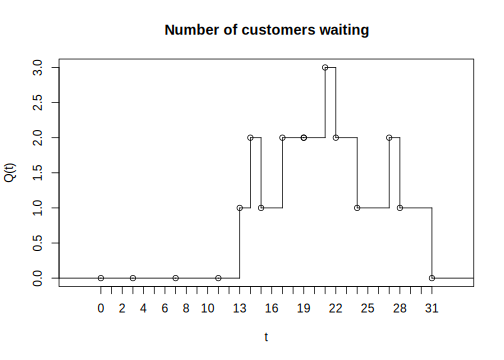
\includegraphics[width=0.7\linewidth]{02-Chapter2_files/figure-latex/NCInQ-1} 

}

\caption{Number of customers waiting in queue for the bank simulation}\label{fig:NCInQ}
\end{figure}

That is, for a given (realized) sample path, \(Q(t)\) is a function that
returns the number of customers in the queue at time \(t\). The mean value
theorem of calculus for integrals states that given a function,
\(f( \bullet )\), continuous on an interval \((a, b)\), there exists a
constant, c, such that

\[\int_{a}^{b}{f\left( x \right)\text{dx}} = f(c)(b - a)\]

\[f\left( c \right) = \frac{\int_{a}^{b}{f\left( x \right)\text{dx}}}{(b - a)}\]

The value, \(f(c)\), is called the mean value of the function. A similar
function can be defined for \(Q(t)\) This function is called the
time-average (and represents the \emph{mean value} of the \(Q(t)\)
function):

\[\overline{Q}\left( n \right) = \frac{\int_{t_{0}}^{t_{n}}{Q\left( t \right)\text{dt}}}{t_{n} - t_{0}}\]

This function represents the \emph{average with respect to time} of the given
state variable. This type of statistical variable is called time-based
because \(Q(t)\) is a function of time.

In the particular case where \(Q(t)\) represents the number of customers
in the queue, \(Q(t)\) will take on constant values during intervals of
time corresponding to when the queue has a certain number of customers. Let \(Q\left( t \right) = \ q_{k}\ \)for\(\ t_{k - 1} \leq t \leq t_{k}\). Then, the time-average can be rewritten as follows:

\[\overline{Q}\left( t \right) = \frac{\int_{t_{0}}^{t_{n}}{Q\left( t \right)\text{dt}}}{t_{n} - t_{0}} = \sum_{k = 1}^{n}\frac{q_{k}(t_{k} - t_{k - 1})}{t_{n} - t_{0}}\]
Note that \(q_{k}(t_{k} - t_{k - 1})\) is the area under the curve, \(Q\left( t \right)\) over the interval \(t_{k - 1} \leq t \leq t_{k}\) and because \[t_{n} - t_{0} = \left( t_{1} - t_{0} \right) + \left( t_{2} - t_{1} \right) + \left( t_{3} - t_{2} \right) + \ \cdots + \left( t_{n - 1} - t_{n - 2} \right) + \ \left( t_{n} - t_{n - 1} \right)\]
we can write,
\[t_{n} - t_{0} = \sum_{k = 1}^{n}{t_{k} - t_{k - 1}}\]

The quantity \(t_{n} - t_{0}\) represents the total time over which the variable is observed. Thus, the time average is simply the area under the curve divided by the amount of time
over which the curve is observed. From this equation, it should be noted
that each value of \(q_{k}\) is weighted by the length of time that the
variable has the value. If we define, \(w_{k} = (t_{k} - t_{k - 1})\),
then we can re-write the time average as:

\[\overline{Q}\left( t \right) = \frac{\int_{t_{0}}^{t_{n}}{Q\left( t \right)\text{dt}}}{t_{n} - t_{0}} = \sum_{k = 1}^{n}\frac{q_{k}(t_{k} - t_{k - 1})}{t_{n} - t_{0}} = \frac{\sum_{k = 1}^{n}{q_{k}w_{k}}}{\sum_{i = 1}^{n}w_{k}}\]

This form of the equation clearly shows that each value of \(q_{k}\) is
weighted by:

\[\frac{w_{k}}{\sum_{i = 1}^{n}w_{k}} = \frac{w_{k}}{t_{n} - t_{0}} = \frac{(t_{k} - t_{k - 1})}{t_{n} - t_{0}}\]

This is why the time average is often called the time-weighted average.
If \(w_{k} = 1\), then the time-weighted average is the same as the sample
average.

Now we can compute the time average for
\(Q\left( t \right),\ N\left( t \right)\) and \(B(t)\). Using the following
formula and noting that \(t_{n} - t_{0} = 31\)

\[\overline{Q}\left( t \right) = \sum_{k = 1}^{n}\frac{q_{k}(t_{k} - t_{k - 1})}{t_{n} - t_{0}}\]

We have that the numerator computes as follows:

\[\sum_{k = 1}^{n}{q_{k}\left( t_{k} - t_{k - 1} \right)} = 0\left( 13 - 0 \right) + \ 1\left( 14 - 13 \right) + \ 2\left( 15 - 14 \right) + \ 1\left( 17 - 15 \right) + \ 2\left( 19 - 17 \right)\]

\[\  + 1\left( 19 - 19 \right) + \ 2\left( 21 - 19 \right) + \ 3\left( 22 - 21 \right) + \ 2\left( 24 - 22 \right) + \ \]

\[1\left( 27 - 24 \right) + \ 2\left( 28 - 27 \right) + \ 1\left( 31 - 28 \right) = 28\]

And, the final time-weighted average number in the queue ss:

\[\overline{Q}\left( t \right) = \frac{28}{31} \cong 0.903\]

The average number in the system and the average number of busy tellers
can also be computed in a similar manner, resulting in:

\[\overline{N}\left( t \right) = \frac{52}{31} \cong 1.677\]

\[\overline{B}\left( t \right) = \frac{24}{31} \cong 0.7742\]

The value of \(\overline{B}\left( t \right)\) is most interesting for this
situation. Because there is only 1 teller, the fraction of the tellers
that are busy is 0.7742. This quantity represents the \emph{utilization} of
the teller. The utilization of a resource represents the proportion of
time that the resource is busy. Let c represent the number of units of a
resource that are available. Then the utilization of the
resource is defined as:

\[\overline{U} = \frac{\overline{B}\left( t \right)}{c} = \frac{\int_{t_{0}}^{t_{n}}{B\left( t \right)\text{dt}}}{c(t_{n} - t_{0})}\]

Notice that the numerator of this equation is simply the total time that
the resource is busy. So, we are computing the total time that the
resource is busy divided by the total time that the resource could be
busy, \(c(t_{n} - t_{0})\), which is considered the utilization.

In the following section, we will explore the basic elements of a process-oriented simulation.

\hypertarget{ch2:ProcessModeling}{%
\section{Elements of Process-Oriented Simulation}\label{ch2:ProcessModeling}}

Chapter \ref{ch1} described
a system as a set of inter-related components that work together to
achieve common objectives. In this chapter, a method for modeling the
operation of a system by describing its processes is presented. In the
simplest sense, a process can be thought of as a sequence of activities,
where an activity is an element of the system that takes an interval of
time to complete. In the bank teller example, the service of the customer
by the teller was an activity. The representation of the dynamic
behavior of the system by describing the process flows of the entities
moving through the system is called process-oriented modeling. When
developing a simulation model using the process-view, there are a number
of terms and concepts that are often used. Before learning some of these
concepts in more detail, it is important that you begin with an
understanding of some of the vocabulary used within simulation. The
following terms will be used throughout the text:

\begin{description}
\item[System]
A set of inter-related components that act together over time to
achieve common objectives.
\item[Parameters]
Quantities that are properties of the system that do not change.
These are typically quantities (variables) that are part of the
environment that the modeler feels cannot be controlled or changed.
Parameters are typically model inputs in the form of variables.
\item[Variables]
Quantities that are properties of the system (as a whole) that
change or are determined by the relationships between the components
of the system as it evolves through time.
\item[System State]
A "snap shot" of the system at a particular point in time
characterized by the values of the variables that are necessary for
determining the future evolution of the system from the present
time. The minimum set of variables that are necessary to describe
the future evolution of the system is called the system's state
variables.
\item[Entity Type]
A class of things (objects) that interact with the system elements. Entity types describe entity instances.
\item[Entity or Entity Instance]
An object of interest in the system whose movement or operation
within the system may cause the occurrence of events. Entities are instances of an Entity Type.
\item[Attribute]
A named property or variable that is associated with an entity type. The value of the attribute is associated with the entity instance described by the entity type.
\item[Event]
An instantaneous occurrence or action that changes the state of the
system at a particular point in time.
\item[Activity]
An interval of time bounded by two events (start event and end
event).
\item[Resource]
A limited quantity of items that are used (e.g.~seized and released)
by entities as they proceed through the system. A resource has a
capacity that governs the total quantity of items that may be
available. All the items in the resource are homogeneous, meaning
that they are indistinguishable. If an entity attempts to seize a
resource that does not have any units available it must wait in a
queue.
\item[Queue]
A location that holds entities when their movement is constrained
within the system.
\item[Future Event List]
A list that contains the time ordered sequence of events for the
simulation.
\end{description}

When developing models, it will be useful to identify the elements of
the system that fit some of these definitions. An excellent place to
develop your understanding of these concepts is with entities because
process-oriented modeling is predicated on describing the life of an
entity as it moves through the system.

\hypertarget{ch2:EntitiesAttributesVariables}{%
\subsection{Entities, Attributes, and Variables}\label{ch2:EntitiesAttributesVariables}}

When modeling a system, there are often many entity types. For
example, consider a retail store. Besides customers, the products might
also be considered as entity types. The products (instances of the entity type) are received by the store
and wait on the shelves until customers select them for purchase.
Entities (entity instances) may come in groups and then are processed individually or they
might start out as individual units that are formed into groups. For
example, a truck arriving to the store may be an entity that consists of
many pallets that contain products. The customers select the products
from the shelves and during the check out process the products are
placed in bags. The customers then carry their bags to their cars.
Entities are uniquely identifiable within the system. If there are two
customers in the store, they can be distinguished by the \emph{values} of
their attributes. For example, considering a product as an entity type, it
may have attributes \emph{serial number}, \emph{weight}, \emph{category}, and \emph{price}.
The set of attributes for a type of entity is called its \emph{attribute
set}. While all products might have these attributes, they do not
necessarily have the same values for each attribute. For example,
consider the following two products:

\begin{itemize}
\item
  (serial number = 12345, weight = 8 ounces, category = green beans,
  price = \$0.87)
\item
  (serial number = 98765, weight = 8 ounces, category = corn, price =
  \$1.12)
\end{itemize}

The products carry or retain these attributes and their values as they
move through the system. In other words, attributes are attached to or
associated with entity types. The values of the attributes for particular entity instances might change
during the operation of the system. For example, a mark down on the
price of green beans might occur after some period of time. Attributes
can be thought of as variables that are attached to entity types.

Not all information in a system is local to the entity types. For example,
the number of customers in the store, the number of carts, and the
number of check out lanes are all characteristics of the system. These
types of data are called \emph{system attributes}. In simulation models, this
information can be modeled with global \emph{variables} or other data modules
(e.g.~resources) to which all entity instances can have access. By making these
quantities visible at the system level, the information can be shared
between the entity instances within the model and between the components of the
system.

Figure~\ref{fig:WarehouseSystem} illustrates the difference between
global (system) variables and entities with their attributes in the
context of a warehouse. In the figure, the trucks are entities with
attributes: arrival time, type of product, amount of product, and load
tracking number. Notice that both of the trucks have these attributes,
but each truck has different \emph{values} for their attributes. The figure
also illustrates examples of global variables, such as, number of trucks
loading, number of trucks unloading, number of busy forklifts, etc. This
type of information belongs to the whole system.

\begin{figure}

{\centering \includegraphics{./figures2/ch2/fig16WarehouseSystem} 

}

\caption{Global variables and attributes within a system}\label{fig:WarehouseSystem}
\end{figure}

Once a basic understanding of the system is accomplished through
understanding system variables, the entities, and their attributes, you
must start to understand the processes within the system. Developing the
process description for the various types of entities within a system
and connecting the flow of entities to the changes in state variables of
the system is the essence of process-oriented modeling. In order for
entities to flow through the model and experience processes, you must be
able to create (and dispose of) the entities. The following section
describes how allows the modeler to create and dispose of entities.

\hypertarget{creating-and-disposing-of-entities}{%
\subsection{Creating and Disposing of Entities}\label{creating-and-disposing-of-entities}}

The basic mechanism by which entity instances are introduced into a model is
the CREATE module. An entity (entity instance) is an object that flows within the model.
As an entity flows through the model it causes the \emph{execution of each
module through which it flows}. Because of this, nothing will happen in
a model unless entities are created. Entities can be used to
represent instances of actual physical objects that move through the
system. For example, in a model of a manufacturing system, entities that
represent the parts that are produced by the system will need to be
created. Sometimes entities do not have a physical representation in the
system and are simply used to represent some sort of logical use. For
example, an entity, whose sole purpose is to generate random numbers or
to read data from an input file, may be created within a model. You will
learn various ways to model with entities as you proceed through the
text.

Figure~\ref{fig:CreateModuleDialog} illustrates the CREATE module
dialog box that opens when double-clicking on the flow chart symbol
within the model window. Understanding what the dialog box entries mean
is essential to writing models. Each dialog box has a Help button
associated with it. Clicking on this button will reveal help files that
explain the basic functionality of the module. In addition, the text
field prompts are explained within the help system.

\begin{figure}

{\centering 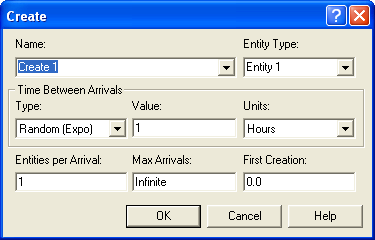
\includegraphics[width=0.55\linewidth,height=0.55\textheight]{./figures2/ch2/fig17CREATEModule} 

}

\caption{CREATE module dialog box}\label{fig:CreateModuleDialog}
\end{figure}

According to the help files, the basic dialog entries are as follows:

\begin{description}
\item[Type]
Type of arrival stream to be generated. Types include: \emph{Random}
(uses an Exponential distribution, user specifies the mean of the
distribution), \emph{Schedule} (specifies a non-homogeneous Poisson
process with rates determined from the specified Schedule module),
\emph{Constant} (user specifies a constant value, e.g., 100), or
\emph{Expression} (pull down list of various distributions or general
expressions written by the user).
\item[Value]
Determines the mean of the exponential distribution (if \emph{Random} is
used) or the constant value (if \emph{Constant} is used) for the time
between arrivals. Applies only when Type is \emph{Random} or \emph{Constant}.
Can be a general expression when the type is specified as
Expression.
\item[Entities per Arrival]
Number of entities that will enter the system at a given time with
each arrival. This allows for the modeling of batch arrivals.
\item[Max Arrivals]
Maximum number of entities that the module will generate. When this
value is reached, the creation of new entities by the module ceases.
\item[First Creation]
Starting time for the first entity to arrive into the system. Does
not apply when Type is \emph{Schedule}.
\end{description}

The CREATE module defines a repeating pattern for an arrival process.
The time between arrivals is governed by the specification of the type
of arrival stream. The time between arrivals specifies an ordered
sequence of events in time at which entities are created and introduced
to the model. At each event, a number of entities can be created. The
number of entities created is governed by the ``Entities per Arrival''
field, which may be stochastic. The first arrival is governed by the
specification of the ``First Creation'' time, which also may be
stochastic. The maximum number of arrival events is governed by the ``Max
Arrivals'' entry. Figure~\ref{fig:TBAPlot} illustrates an arrival process where the
time of the first arrival is given by T1, the time of the second arrival
is given by T1 + T2, and the time of the third arrival is given by T1 +
T2 + T3. In the figure, the number of arriving entities at each arriving
event is given by N1, N2, and N3 respectively.

\begin{figure}

{\centering 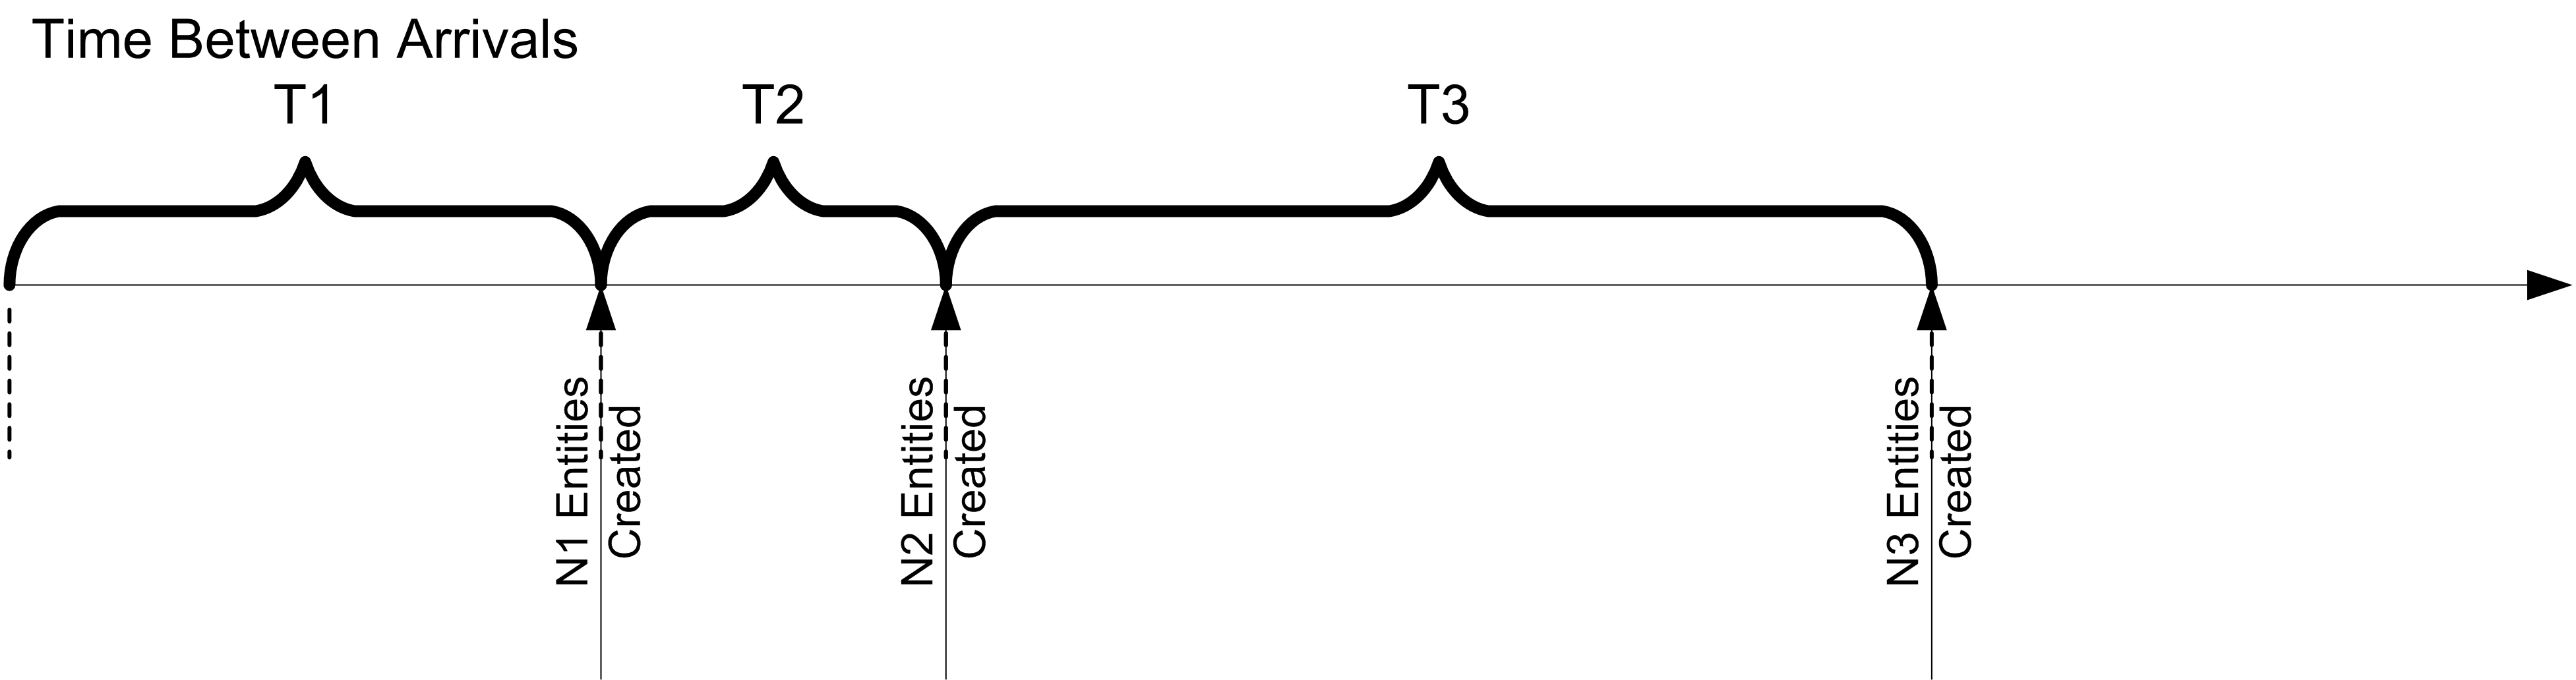
\includegraphics{./figures2/ch2/fig18TBAPlot} 

}

\caption{Example arrival process}\label{fig:TBAPlot}
\end{figure}

A CREATE module works by scheduling a future event to occur according to the specified pattern. At each occurrence of the event, a new instance of the entity type is created. The instance is called an entity. The entity instance then executes additional modules until the entity instance hits a module that blocks its progress. More details of how this process works is provided in Section \ref{ch2:howArenaWorks}. The CREATE module continues scheduling the next creation event until the maximum number of creation events is reached or the simulation ends. A common creation process is the Poisson arrival process.

To specify a Poisson arrival process with mean rate
\(\lambda\), a CREATE module as shown in
Figure~\ref{fig:PoissonCreateModule} can be used. Why does this specify a Poisson
arrival process? Because the time between arrivals for a Poisson process
with rate \(\lambda\) is exponentially distributed with the mean of the
exponential distribution being \(1/\lambda\).

\begin{figure}

{\centering 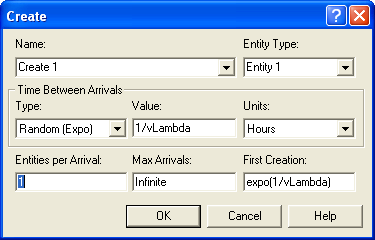
\includegraphics[width=0.55\linewidth,height=0.55\textheight]{./figures2/ch2/fig19PoissonCreateModule} 

}

\caption{CREATE module for Poisson process}\label{fig:PoissonCreateModule}
\end{figure}

To specify a compound arrival process, use the ``Entities per Arrival''
field. For example, suppose you have a compound Poisson process
where the distribution for the number created at each arrival is
governed by a discrete distribution. See \citep{ross1997introduction} for more information on the theory of compound Poisson processes.

\[P(X = x) = \left\{ 
   \begin{array}{ll}
     0.2 & \quad \text{x = 1}\\
     0.3 & \quad \text{x = 2}\\
     0.5 & \quad \text{x = 3}
   \end{array} \right.\]

Figure~\ref{fig:CompoundPoissonCreateModule} shows the CREATE module for this
compound Poisson process with the entities per arrival field using the
DISC(0.2, 1, 0.5, 2, 1.0, 3) discrete empirical distribution function.

When developing models, it is often useful to create one entity and use
that entity to trigger other actions in the model. For example, to read
in information from a file, a logical entity can be created at time zero
and used to execute a READ module. To create one and only one entity at
time zero, specify the \emph{Max Arrivals} field as one, the \emph{First Creation}
field as 0.0, the \emph{Entities per Arrival} as one, and the type field as
Constant. The value specified for the constant will be immaterial since
only one entity will be created.

\begin{figure}

{\centering 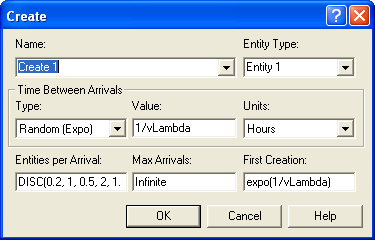
\includegraphics[width=0.55\linewidth,height=0.55\textheight]{./figures2/ch2/fig20CompoundPoissonCreate} 

}

\caption{CREATE module for compound Poisson process}\label{fig:CompoundPoissonCreateModule}
\end{figure}

Each entity that is created allocates memory for the entity. Once the
entity has traveled through its process within the model, the entity
should be disposed. The DISPOSE module acts as a ``sink'' to dispose of
entities when they are no longer needed within the model.

\begin{figure}

{\centering 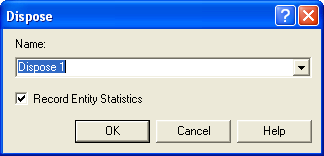
\includegraphics[width=0.5\linewidth,height=0.5\textheight]{./figures2/ch2/fig21DisposeModule} 

}

\caption{DISPOSE module dialog box}\label{fig:DisposeModule}
\end{figure}

Figure~\ref{fig:DisposeModule} illustrates the dialog box for the
DISPOSE module. The DISPOSE module indicates the number of entities that
are disposed by the module within the animation. In addition, the
default action is to record the entity statistics prior to disposing the
entity. If the Entities Statistics Collection field is checked within
the Project Parameters tab of the Run/Setup dialog, the entity
statistics will include VA Time (value added time), NVA Time (non-value
added time), Wait Time, Transfer Time, Other Time and entity Total Time.
If the Costing Statistics Collection field is also checked within the
Project Parameters tab of the Run/Setup dialog, additional entity
statistics include VA Cost (value added cost), NVA Cost (non-value added
cost), Wait Cost, Transfer Cost, Other Cost, and Total Cost.
Additionally, the number of entities leaving the system (for a given
entity type) and currently in the system (WIP, work in process) will be
tabulated. These cost allocations assume an activity based costing model which is beyond the scope of this chapter.

You now know how to introduce entities into a model and how to dispose
of entities after you are done with them. To make use of the entities
within the model, you must first understand how to define and use
variables and entity attributes within a model.

\hypertarget{defining-variables-and-attributes}{%
\subsection{Defining Variables and Attributes}\label{defining-variables-and-attributes}}

In a programming language like C, variables must first be defined before
using them in a program. For example, in C, a variable named x can be
defined as type float and then used in assignment statements such as:
\emph{float x; x = x + 2;}

Variables in standard programming languages have a specific scope
associated with their execution. For example, variables defined within a
function are limited to use within that function. Global variables that
can be used throughout the entire program may also be defined.

In , \emph{all variables are global}. You can think of variables as belonging
to the system being modeled. Everything in the system can have access to
the variables of the system. Variables provide a named location in
computer memory that persists until changed during execution. The naming
conventions for declaring variables in are quite liberal. This can be
both a curse and a blessing. Because of this, you should adopt a
standard naming convention when defining variables. The models in this
text try to start the name of all variables with the letter ``v''. For
example, in the previously discussed CREATE module examples, the
variable \emph{vLambda} was used to represent the arrival rate of the Poisson
process. This makes it easy to distinguish variables from other
constructs when reviewing, debugging, and documenting the model.

In addition, the naming rules allow the use of spaces within a variable
name, e.g.~\emph{This is a legal name} is a legally named variable.
Suppose you needed to count the number of parts and decided to name your
variable \emph{Part Count}. The use of spaces in this manner should be
discouraged because woe unto you if you have this problem: \emph{Part Count}
and \emph{Part Count}. Can you see the problem? The second variable \emph{Part
Count} has extra spaces between \emph{Part} and \emph{Count}. Try searching
through every dialog box to find that in a model!

According to the naming convention recommended here, you would name this
variable \emph{vPartCount}, concatenating and capitalizing the individual
components of the name. Of course you are free to name your variables
whatever you desire as long as the names do not conflict with already
existing variables or keywords within Arena. To learn more about the
specialized variables available within Arena, you should refer to the
portable document file (PDF) document \emph{Variables Guide}, which comes
with the installation. Reading this document should give you a better
feeling for the functional capabilities of Arena.

To declare variables, you use the VARIABLE module found in the Basic
Process template. The VARIABLE module is a data module and is accessed
either through the spreadsheet view (Figure~\ref{fig:VariableSheetView}) or through a dialog box (Figure~\ref{fig:VariableDialogBox}).

\begin{figure}

{\centering 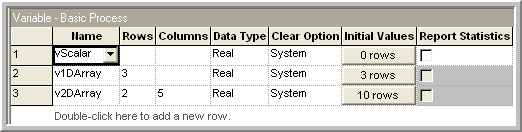
\includegraphics[width=0.8\linewidth,height=0.8\textheight]{./figures2/ch2/fig22VariableSheetView} 

}

\caption{Data sheet view of VARIABLE data module}\label{fig:VariableSheetView}
\end{figure}

\begin{figure}

{\centering 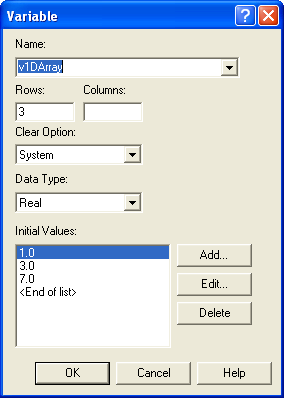
\includegraphics[width=0.45\linewidth,height=0.45\textheight]{./figures2/ch2/fig23VariableDialogBox} 

}

\caption{Dialog box for defining variables}\label{fig:VariableDialogBox}
\end{figure}

Variables can be scalars or can be defined as arrays. The
arrays can be either 1-dimensional or 2-dimensional. For 1-dimensional
arrays, you specify either the number of rows or the number of columns.
There is no difference between an array specified with, say 3 rows, or
an array specified with 3 columns. The net effect is that there will be
three variables defined which can be indexed by the numbers 1, 2, and 3.
When defining a 2-dimensional array of variables (see Figure \ref{fig:SpreadSheetArray}), you specify the number
of rows and columns. Array indexes start at 1 and run through the size
of the specified dimension. A runtime error will occur if the index used
to access an array is not within the bounds of the array's dimensions.

\begin{figure}

{\centering 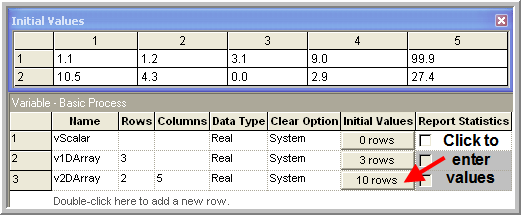
\includegraphics[width=0.8\linewidth,height=0.8\textheight]{./figures2/ch2/fig24SpreadSheetArray} 

}

\caption{Data sheet view for 2-D variable array}\label{fig:SpreadSheetArray}
\end{figure}

When defining a variable or an array of variables, you may specify the initial value(s). The default initial value for all variables is
zero. By using the spreadsheet view within the Data window, see
Figure~\ref{fig:VariableSheetView}, you can easily enter the initial
values for variables and arrays. All variables are treated as real
numbers. If you need to represent an integer, e.g.~\emph{vPartCount},
you simply represent it as a variable. There is no specific integer data type.

It is important to remember that all variables or arrays are global
within Arena. Variables are used to share information across all modules
within the model. You should think of variables as characteristics or
properties of the model as a whole. Variables belong to the entire
system being modeled.

Arena has another data type that is capable of holding values called an
attribute. An attribute is a named property or characteristic of an
entity. For example, suppose the time to produce a part depends on the
dimensions or area associated with the part. A CREATE module can be used
to create entities that represent the parts. After the parts are
created, the area associated with each part needs to be set. Each part
created could have different values for its area attribute.

\begin{itemize}
\item
  Part 1: area = 5 square inches
\item
  Part 2: area = 10 square inches
\end{itemize}

Part 1 and part 2 have the same named attribute, area, but the value for
this attribute is different for each part.

For those readers familiar with object-oriented programming, attributes
in are similar in \emph{concept} to attributes associated with objects in
languages such as VB.Net, Java, and C++. If you understand the use of
attributes in those languages, then you have a basis for how attributes
can be used within . When an instance of an entity is created within ,
it is like creating an object in an object-oriented language. The object
instance has attributes associated with it. You can think of an entity
as a record or a row of data that is associated with that particular
object instance. Each row represents a different entity.

\hypertarget{tab:EntityRecords}{}
\begin{longtable}[]{@{}lcccc@{}}
\caption{\label{tab:EntityRecords} Entities conceptualized as records}\tabularnewline
\toprule
IDENT & Entity.SerialNumber & Size & Weight & ProcessingTime\tabularnewline
\midrule
\endfirsthead
\toprule
IDENT & Entity.SerialNumber & Size & Weight & ProcessingTime\tabularnewline
\midrule
\endhead
1 & 1001 & 2 & 33 & 20\tabularnewline
2 & 1002 & 3 & 22 & 55\tabularnewline
3 & 1003 & 1 & 11 & 44\tabularnewline
4 & 1001 & 2 & 33 & 20\tabularnewline
5 & 1004 & 5 & 10 & 14\tabularnewline
6 & 1005 & 4 & 14 & 10\tabularnewline
\bottomrule
\end{longtable}

Table~\ref{tab:EntityRecords} presents six entities conceptualized as
records in a table. You can think of the creation and disposing of entities as
adding and deleting records within the model's ``entity table''. The column IDENT represents the IDENT attribute, which uniquely identifies each entity (instance). IDENT is a special pre-defined
attribute that is used to uniquely track entities currently in the model.
The IDENT attribute is assigned when the entity is created. When an
entity is created, memory is allocated for the entity and all of
its attributes. A different value for IDENT is assigned to each entity
that currently exists within the model. When an entity is disposed, the
memory associated with that entity is released and the \emph{values} for
IDENT will be reused for newly created entities. Thus, the IDENT
attribute uniquely identifies entities \emph{currently} in the model. No two
entities currently in the model have the same value for the IDENT
attribute. Think of IDENT as the primary key into the entity record table.

Every entity in the model has a unique row in the table to store its attribute
values. \emph{Entity.SerialNumber} is just one of those attributes. The
\emph{Entity.SerialNumber} attribute is also a number assigned to an
entity instance when it is created; however, if the entity is ever duplicated
(cloned) in the model, the clones will have the same value for the
\emph{Entity.SerialNumber} attribute. When an entity is cloned (duplicated) all attributes \emph{except} IDENT are duplicated. Entity.SerialNumber will not be unique when entities are
cloned. IDENT can be used to uniquely identify an entity.
Entity.SerialNumber can be used to identity entities that have the same
serial number. In other words, all duplicates of an entity instance. In the table, there are two entities (1 and 4) that are duplicates of each other. The duplication of entities
will be discussed later in this chapter. The size, weight, and
processing time attributes are three \emph{user defined} attributes
associated with each of the entities. To find a description of the full
list of pre-defined entity attributes, do a search on "Attributes and
Entity-Related Variables" in the Help system.

When you define a user-defined attribute, you are adding another
``column'' to the ``entity table''. The implication of this statement is
very important. The defining of a user-defined attribute associates that
attribute with \emph{every} entity type. This is quite different than what
you see in object-oriented languages where you can associate specific
attributes with specific classes (types) of objects. Within Arena, an entity type is an
entity type. You can specify attributes that can allow you to conceptualize
them as being different. This is conceptually defining the attribute set
for the entity type that was previously mentioned. For example, you
might create entities and think of them as parts flowing in a
manufacturing system. Within a manufacturing system, there might also be
entities that represent pallets that assist in material handling within
the system. A part may have a processing time attribute and a pallet may
have a move time attribute.

\hypertarget{tab:EntityTypeRecords}{}
\begin{longtable}[]{@{}lccccc@{}}
\caption{\label{tab:EntityTypeRecords} Different types of entities conceptualized as records}\tabularnewline
\toprule
IDENT & Type & Size & Weight & MoveTime & ProcessingTime\tabularnewline
\midrule
\endfirsthead
\toprule
IDENT & Type & Size & Weight & MoveTime & ProcessingTime\tabularnewline
\midrule
\endhead
1 & 1 & 2 & 33 & ------- & 20\tabularnewline
2 & 1 & 3 & 22 & ------- & 55\tabularnewline
3 & 2 & 1 & 11 & 23 & -------\tabularnewline
\bottomrule
\end{longtable}

In Table~\ref{tab:EntityTypeRecords}, the type attribute indicates the
type of entity (part = 1, pallet = 2). Notice that all entities have the
move time and processing time attributes \emph{defined}. These attributes can
be used regardless of the actual type of entity. In using attributes
within Arena, it is up to the modeler to provide the appropriate context
(understanding of the attribute set) for an entity instance and then to use the
attributes and their values appropriately within that context.

There are two ways to distinguish between different types of entities.
Each entity has a pre-defined attribute, called \emph{Entity.Type}, which can be used to
set the type of the entity. In addition, you can specify a user defined
attribute to indicate the type of the entity. Arena's on-line help has
this to say about the \emph{Entity.Type} attribute:

\begin{quote}
\emph{Entity.Type} This attribute refers to one of the types (or names) of
entities defined in the Entities element. Entity type is used to set
initial values for the entity picture and the cost attributes. It is
also used for grouping entity statistics (e.g.~each entity's
statistics will be reported as part of all statistics for entities of
the same type).
\end{quote}

The Entity module in the Basic process panel allows you to define entity
types. The dialog box shown in
Figure~\ref{fig:EntityModule} shows the basic text fields for
defining an entity type. The most important field is the "Entity Type"
field, which gives the name of the entity type. The \emph{Initial Picture}
field allows a picture to be assigned to the \emph{Entity.Picture} attribute
when entities of this type are created. The other fields refer to how
costs are tabulated for the entity when applying activity based costing
(ABC) functionality. This functionality is discussed in Section \ref{app:ArenaMisc:ArenaCosting}.

\begin{figure}

{\centering 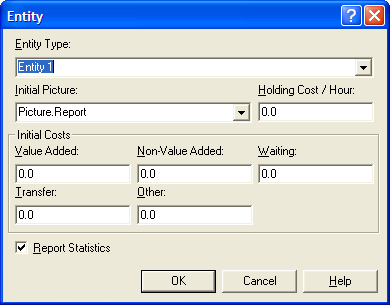
\includegraphics[width=0.55\linewidth,height=0.55\textheight]{./figures2/ch2/fig25EntityModule} 

}

\caption{Entity module dialog box}\label{fig:EntityModule}
\end{figure}

The advantage of using the \emph{Entity.Type} attribute is that some automated
functions become easier, such as collecting statistics by entity type
(via the DISPOSE module), activity based costing, and displaying the
entity picture. Using the \emph{Entity.Type} attribute makes it a little more
difficult to randomly assign an entity type to an entity, although this
can still be done using the set concept, which will be discussed in a later chapter.\\
By using a user defined attribute, you can change and interpret the
attribute very easily by mapping a number to the type as was done in
Table~\ref{tab:EntityTypeRecords}.

Now that a basic understanding of the concept of an entity attribute has
been developed, you still need to know how to declare and use the
attributes. The declaration and use of attributes in is similar to how
variables can be declared and used in Visual Basic. Unless you have the
\emph{Option Explicit} keyword specified for Visual Basic, any variables can
be declared upon their first use. For attributes in this also occurs.
For example, to make an attribute called \emph{myArea} available simply use
it in a module, such as an ASSIGN module. This does cause difficulties
in debugging. It is also recommended that you adopt a naming convention
for your attributes. This text uses the convention of placing ``my'' in
front of the name of the attribute, as in \emph{myArea}. This little mnemonic
indicates that the attribute belongs to the entity. In addition, spaces
within the name are not used, and the convention of the concatenation
and the capitalization of the words within the name is used. Of course,
you are free to label your attributes whatever you desire as long as the
names do not conflict with already existing attributes or keywords
within Arena. Attributes can also be formally declared using the ATTRIBUTES
module. This also allows the user to define attributes that are arrays. Using the ATTRIBUTEs module is the preferred method for defining attributes because comments can be provided for the attribute and pre-defining attributes facilitates their selection within drop down text fields or when using the expression builder. This approach tends to avoid annoying syntax errors.

\hypertarget{modeling-a-simple-discrete-event-dynamic-system}{%
\section{Modeling a Simple Discrete-Event Dynamic System}\label{modeling-a-simple-discrete-event-dynamic-system}}

This section presents how to model a system in which the state changes
at discrete events in time as discussed in the previous section.

\hypertarget{ch2:DriveThruPharmacy}{%
\subsection{A Drive through Pharmacy}\label{ch2:DriveThruPharmacy}}

This example considers a small pharmacy that has a single line for
waiting customers and only one pharmacist. Assume that customers arrive
at a drive through pharmacy window according to a Poisson distribution
with a mean of 10 per hour. The time that it takes the pharmacist to
serve the customer is random and data has indicated that the time is
well modeled with an exponential distribution with a mean of 3 minutes.
Customers who arrive to the pharmacy are served in the order of arrival
and enough space is available within the parking area of the adjacent
grocery store to accommodate any waiting customers.

The drive through pharmacy system can be conceptualized as a single
server waiting line system, where the server is the pharmacist. An
idealized representation of this system is shown in
Figure~\ref{fig:DriveThru}. If the pharmacist is busy serving a
customer, then additional customers will wait in line. In such a
situation, management might be interested in how long customers wait in
line, before being served by the pharmacist. In addition, management
might want to predict if the number of waiting cars will be large.
Finally, they might want to estimate the utilization of the pharmacist
in order to ensure that the pharmacist is not too busy.

\begin{figure}

{\centering 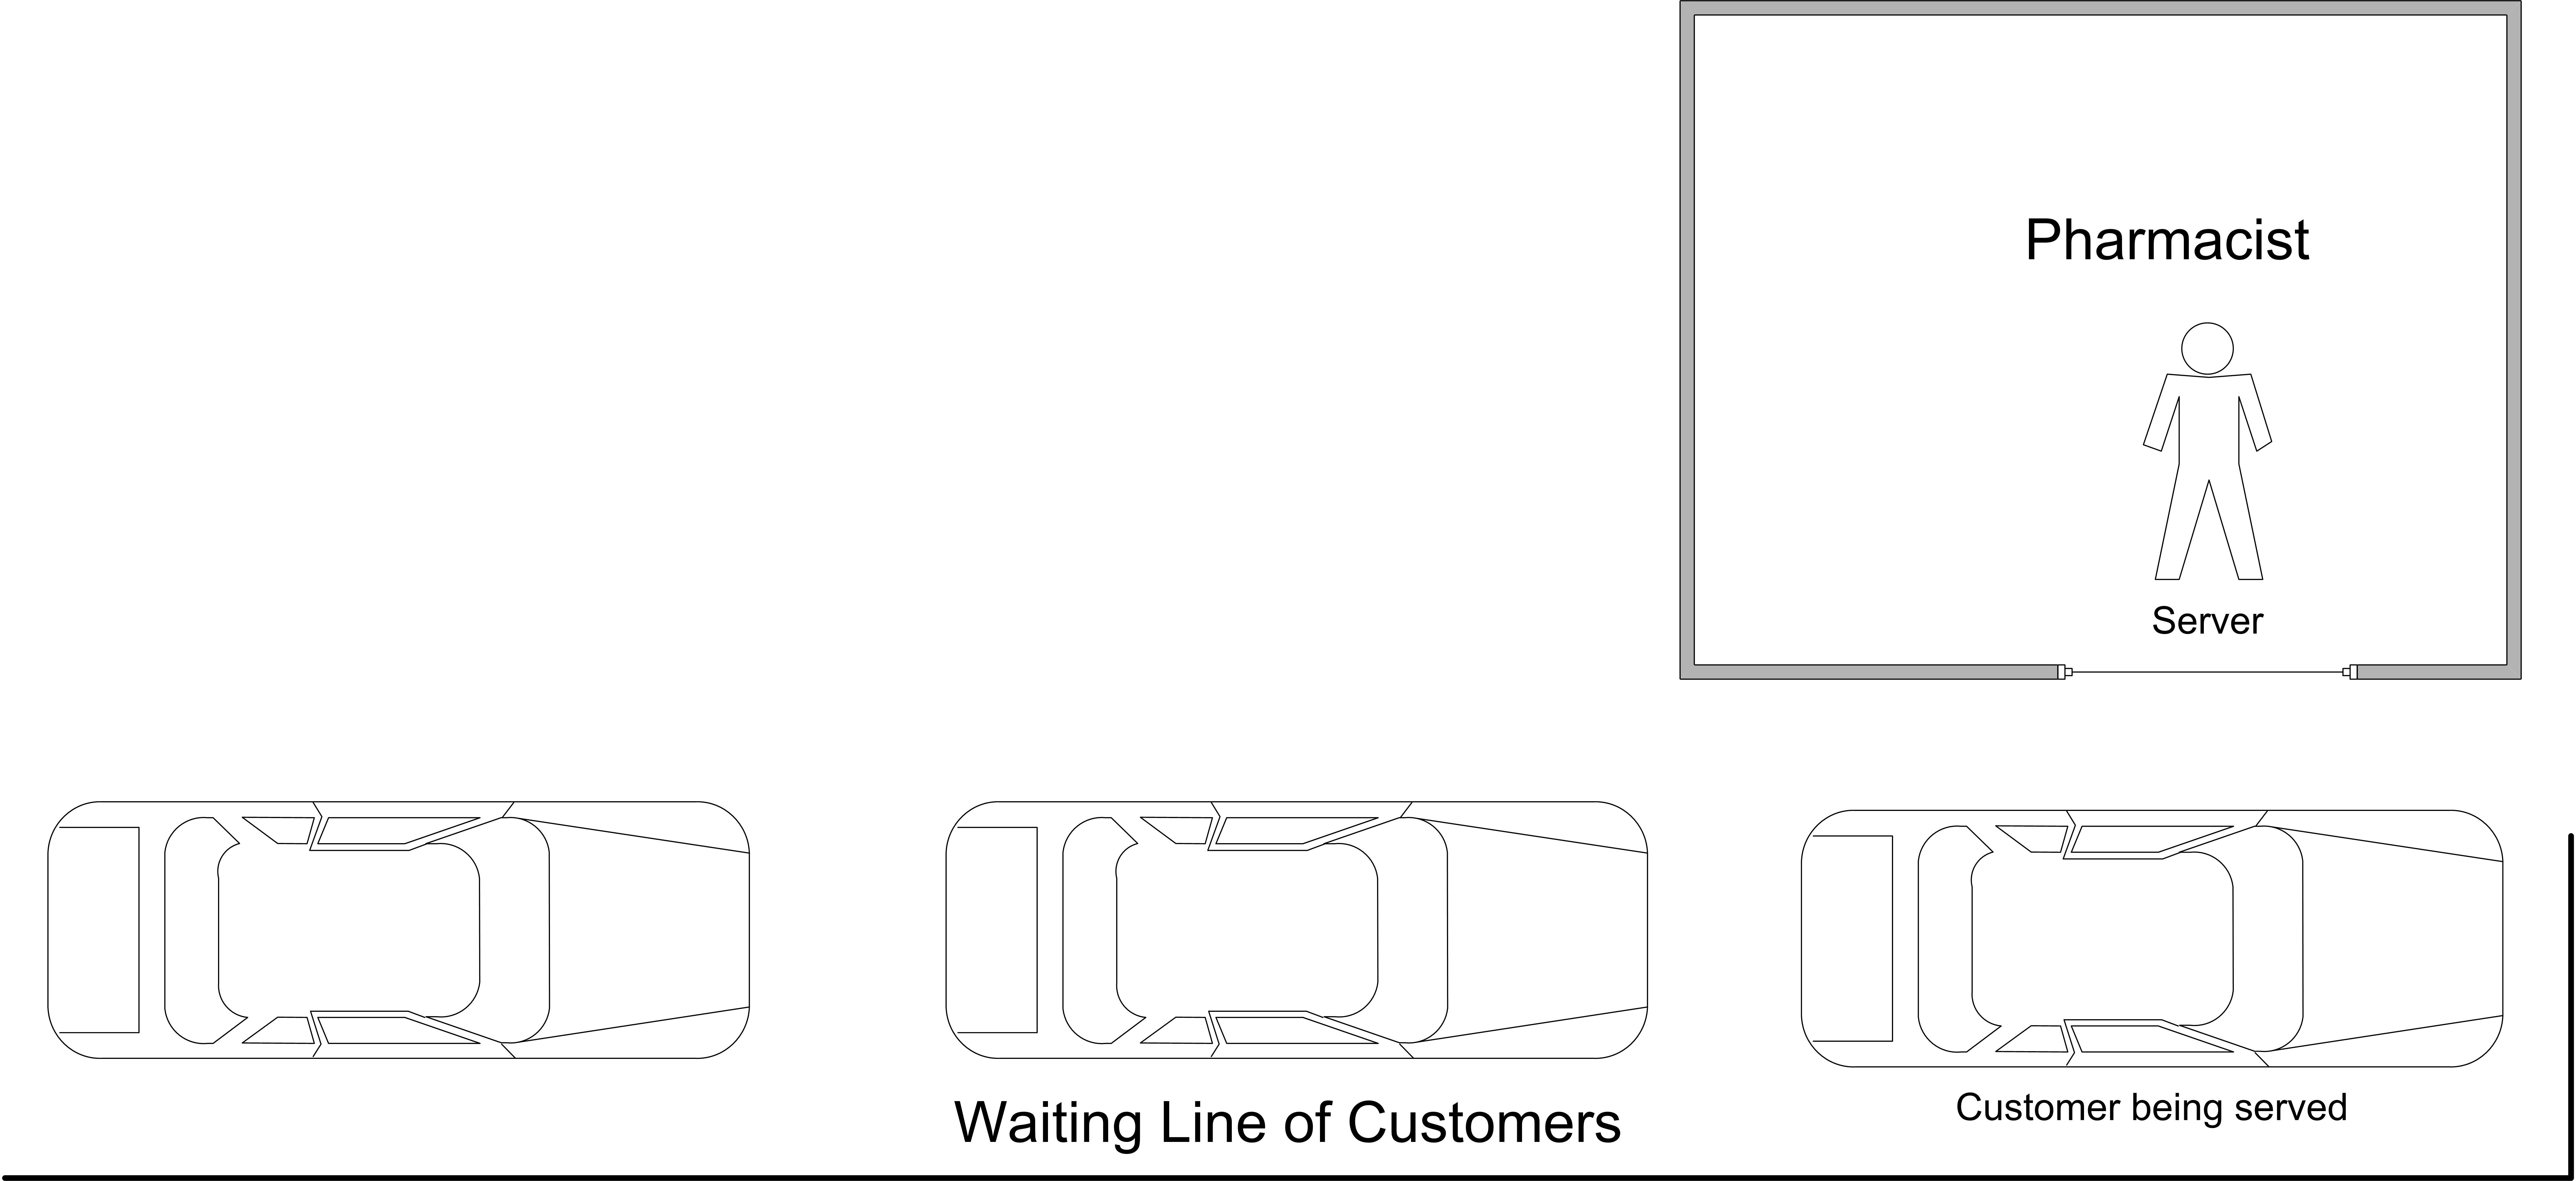
\includegraphics[width=0.8\linewidth,height=0.8\textheight]{./figures2/ch2/fig26DriveThruPharmacy} 

}

\caption{Simple drive through pharmacy}\label{fig:DriveThru}
\end{figure}

\hypertarget{ch2:ModelingThePharmacy}{%
\subsection{Modeling the System}\label{ch2:ModelingThePharmacy}}

Process modeling is predicated on modeling the process flow of "entities" through a
system. Thus, the first question to ask is: \emph{What is the system}? In
this situation, the system is the pharmacist and the potential customers
as idealized in Figure~\ref{fig:DriveThru}. Now you should consider the entities of
the system. An entity is a conceptual thing of importance that flows
through a system potentially using the resources of the system.
Therefore, one of the first questions to ask when developing a model
is: \emph{What are the entities}? In this situation, the entities are the
customers that need to use the pharmacy. This is because customers are
discrete things that enter the system, flow through the system, and then
depart the system.

Since entities often use things as they flow through the system, a
natural question is to ask: \emph{What are the resources that are used by the
entities}? A resource is something that is used by the entities and that
may constrain the flow of the entities within the system. Another way to
think of resources is to think of the things that provide service in the
system. In this situation, the entities ``use'' the pharmacist in order to
get their medicine. Thus, the pharmacist can be modeled as a resource.

Since we are modeling the process flows of the entities
through a system, it is natural to ask: \emph{What are the process flows}? In
answering this question, it is conceptually useful to pretend that you
are an entity and to ask: \emph{What to I do}? In this situation, you can
pretend that you are a pharmacy customer. \emph{What does a customer do}?
Arrive, get served, and leave. As you can see, initial modeling involves
identifying the elements of the system and what those elements do. The
next step in building a simulation model is to enhance your conceptual
understanding of the system through conceptual modeling. For this simple
system, very useful conceptual model has already been given in
Figure~\ref{fig:DriveThru}. As you proceed through this text, you will
learn other conceptual model building techniques. From the conceptual
modeling, you might proceed to more logical modeling in preparation for
using . A useful logical modeling tool is to develop pseudo-code for the
situation. Here is some potential pseudo-code for this situation.

\begin{itemize}
\item
  Create customers according to Poisson arrival process
\item
  Process the customers through the pharmacy
\item
  Dispose of the customers as they leave the system
\end{itemize}

The pseudo-code represents the logical flow of an entity (customer)
through the drive through pharmacy: Arrive (create), get served
(process), leave (dispose).

Another useful conceptual modeling tool is the \emph{activity diagram}. An
\emph{activity} is an operation that takes time to complete. An activity is
associated with the state of an object over an interval of time.
Activities are defined by the occurrence of two events which represent
the activity's beginning time and ending time and mark the entrance and
exit of the state associated with the activity. An activity diagram is a
pictorial representation of the process (steps of activities) for an
entity and its interaction with resources while within the system. If
the entity is a temporary entity (i.e.~it flows through the system) the
activity diagram is called an activity flow diagram. If the entity is
permanent (i.e.~it remains in the system throughout its life) the
activity diagram is called an activity cycle diagram. The notation of an
activity diagram is very simple, and can be augmented as needed to
explain additional concepts:

\begin{description}
\item[Queues]
shown as a circle with queue labeled inside
\item[Activities]
shown as a rectangle with appropriate label inside
\item[Resources]
shown as small circles with resource labeled inside
\item[Lines/arcs]
indicating flow (precedence ordering) for engagement of entities in
activities or for obtaining resources. Dotted lines are used to
indicate the seizing and releasing of resources.
\item[zigzag lines]
indicate the creation or destruction of entities
\end{description}

Activity diagrams are especially useful for illustrating how entities
interact with resources. Activity diagrams are easy to build by hand and
serve as a useful communication mechanism. Since they have a simple set
of symbols, it is easy to use an activity diagram to communicate with
people who have little simulation background. Activity diagrams are an
excellent mechanism to document your conceptual model of the system
before building the model in .

\begin{figure}

{\centering 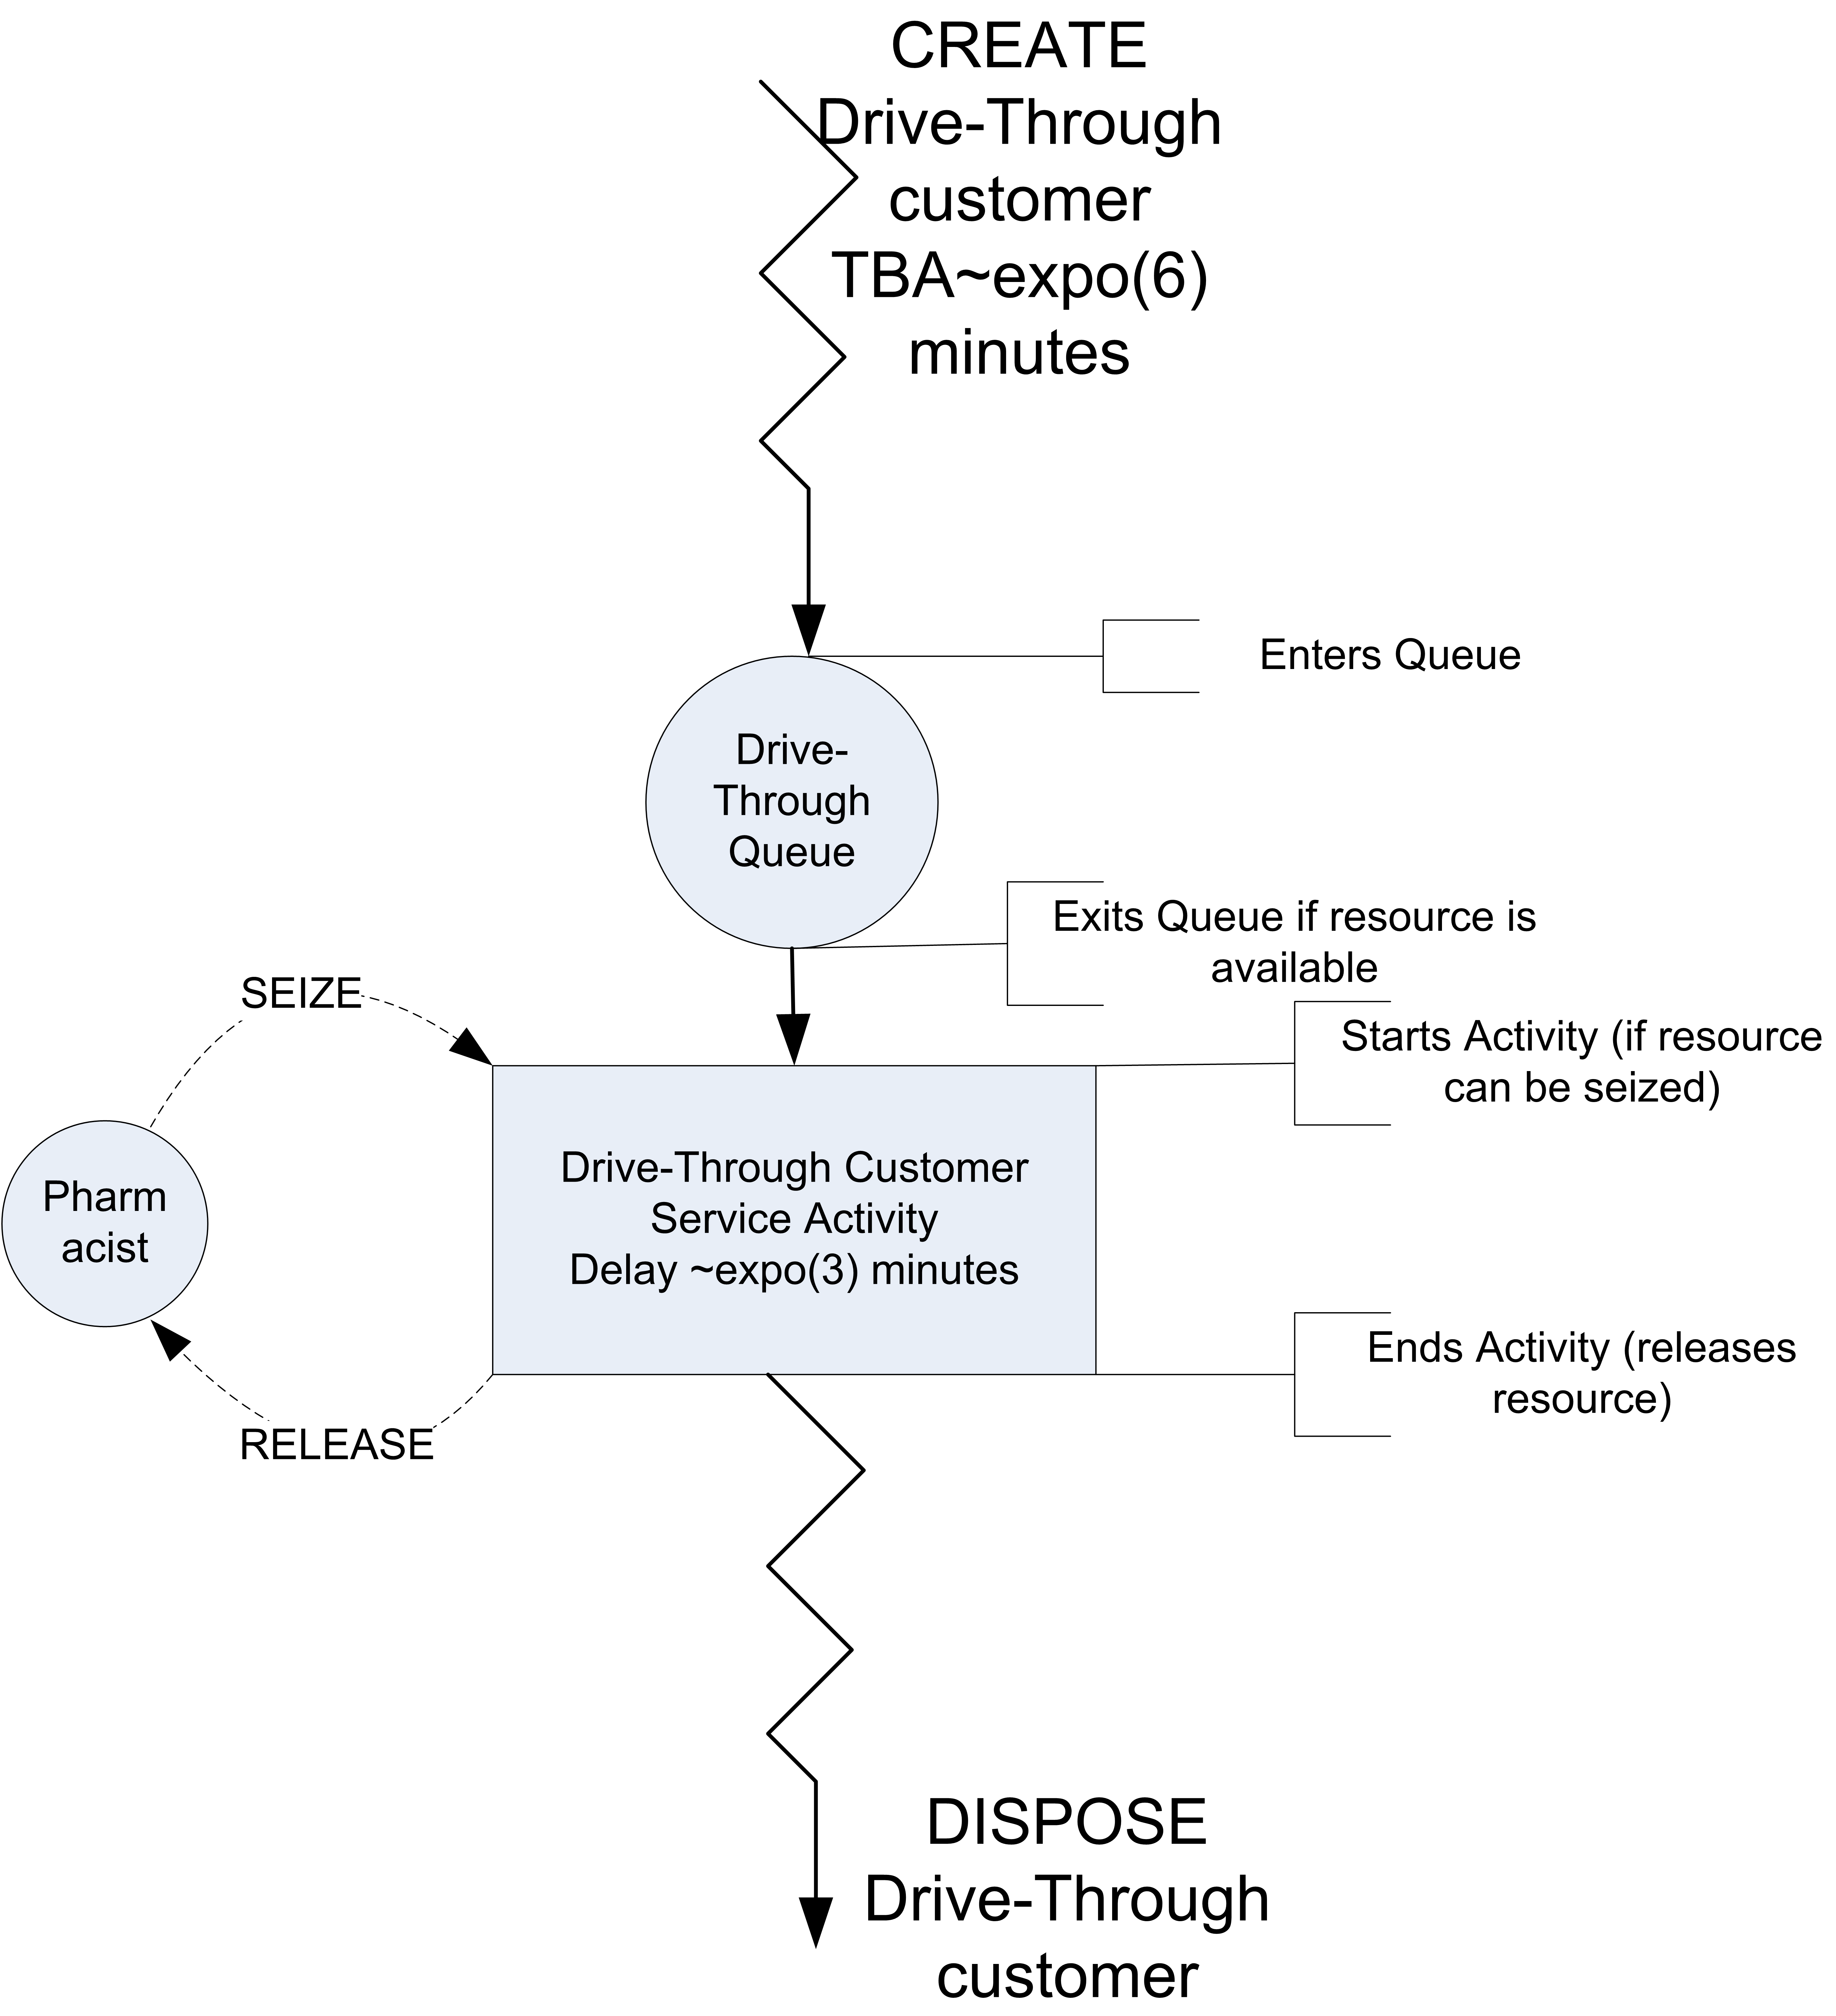
\includegraphics[width=0.6\linewidth,height=0.6\textheight]{./figures2/ch2/fig27ActivityDiagram} 

}

\caption{Activity diagram for drive through pharmacy}\label{fig:ActivityDiagram}
\end{figure}

Figure~\ref{fig:ActivityDiagram} shows the activity diagram for the
pharmacy situation. This diagram was built using Visio software and the
drawing is available with the supplemental files for this chapter. You
can use this drawing to copy and paste from, in order to form other
activity diagrams, but I recommend just drawing activity diagrams free-hand.

An activity diagram describes the life of an entity within
the system. The zigzag lines at the top of the diagram indicate the
creation of an entity. While not necessary, the diagram has been
augmented with like pseudo-code to represent the CREATE statement.
Consider following the life of the customer through the pharmacy.
Following the direction of the arrows, the customers are first created
and then enter the queue. Notice that the diagram clearly shows that
there is a queue for the drive-through customers. You should think of
the entity flowing through the diagram. As it flows through the queue,
the customer attempts to start an activity. In this case, the activity
requires a resource. The pharmacist is shown as a resource (circle) next
to the rectangle that represents the service activity.

The customer requires the resource in order to start its service
activity. This is indicated by the dashed arrow from the pharmacist
(resource) to the top of the service activity rectangle. If the customer
does not get the resource, they wait in the queue. Once they receive the
number of units of the resource requested, they proceed with the
activity. The activity represents a delay of time and in this case the
resource is used throughout the delay. After the activity is completed,
the customer releases the pharmacist (resource). This is indicated by
another dashed arrow, with the direction indicating that the resource is
"being put back" or released. After the customer completes its service
activity, the customer leaves the system. This is indicated with the
zigzag lines going to no-where and augmented with the keyword DISPOSE.
The dashed arrows of a typical activity diagram have also been augmented
with the like pseudo-code of SEIZE and RELEASE. The conceptual model of
this system can be summarized as follows:

\begin{description}
\item[System]
The system has a pharmacist that acts as a resource, customers that
act as entities, and a queue to hold the waiting customers. The
state of the system includes the number of customers in the system,
in the queue, and in service.
\item[Events]
Arrivals of customers to the system, which occur within an
inter-event time that is exponentially distributed with a mean of 6
minutes.
\item[Activities]
The service time of the customers are exponentially distributed with
a mean of 3 minutes.
\item[Conditional delays]
A conditional delay occurs when an entity has to wait for a
condition to occur in order to proceed. In this system, the customer
may have to wait in a queue until the pharmacist becomes available.
\end{description}

With an activity diagram and pseudo-code such as this available to
represent a solid conceptual understanding of the system, you can begin
the model development process.

\begin{figure}

{\centering 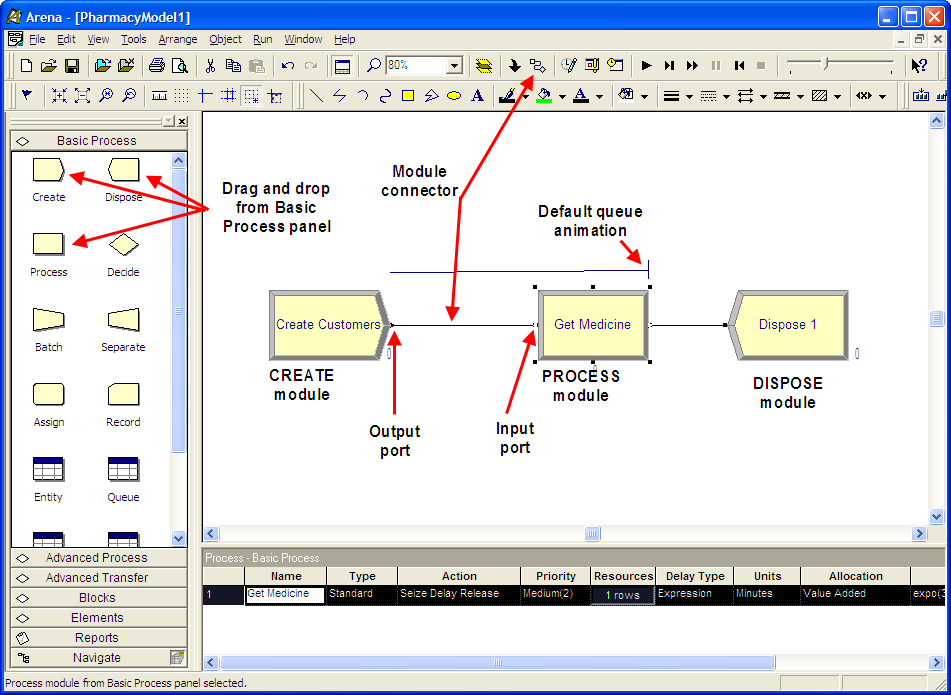
\includegraphics[width=0.8\linewidth,height=0.8\textheight]{./figures2/ch2/fig28OverviewDriveThruArenaModel} 

}

\caption{Overview of pharmacy model}\label{fig:DriveThruOverview}
\end{figure}

\hypertarget{ch2:PM:Implementation}{%
\subsection{Pharmacy Model Implementation}\label{ch2:PM:Implementation}}

Now, you are ready to implement the conceptual model. If you
haven't already done so, open up the Arena Environment. Using the Basic
Process Panel template, drag the CREATE, PROCESS, and DISPOSE modules
into the model window and make sure that they are connected as shown in
Figure~\ref{fig:DriveThruOverview}. In order to drag and drop the modules,
simply select the module within the Basic Process template and drag the
module into the model window, letting go of the mouse when you have
positioned the module in the desired location. If the module within the
model window is highlighted (selected), the next dragged module will
automatically be connected. If you placed the modules and they weren't
automatically connected, then you can use the connect toolbar icon.
Select the icon and then select the ``from" module near the connection
exit point and then holding the mouse button down drag to form a
connection line to the entry point of the''to" module. The names of the
modules will not match what is shown in the figure. You will name the
modules as you fill out their dialog boxes.

\hypertarget{ch2:PM:Arrivals}{%
\subsection{Specify the Arrival Process}\label{ch2:PM:Arrivals}}

Within Arena nothing happens unless entities enter the model. This is done
through the use of the CREATE module. Actually, this statement is not quite true and not quite false. You don't necessarily have to have a CREATE module in the model to get things to happen, but this requires the use of advanced techniques that are beyond the scope of this book. In the current example, pharmacy
customers arrive according to a Poisson process with a mean of \(\lambda\)
= 10 per hour. According to probability theory, this implies that the
time between arrivals is exponentially distributed with a mean of
(\(1/\lambda\)). Thus, for this situation, the mean time between arrivals is 6 minutes.

\begin{equation}
\frac{1}{\lambda} = \frac{\text{1 hour}}{\text{10 customers}} \times \frac{\text{60 minutes}}{\text{1 hour}} = \frac{\text{6 minutes}}{\text{customer}}
\label{eq:rateConversion}
\end{equation}

\begin{rmdwarning}
\textbf{Do not make the mistake of using the arrival rate within the CREATE module} The CREATE module uses the time between arrivals. Convert your arrival rate to the time between arrivals as shown in Equation \eqref{eq:rateConversion}.
\end{rmdwarning}

Open up the CREATE module (by double clicking on it) and fill it in as
shown in Figure \ref{fig:PMCreateModule}. The distribution for the ``Time Between
Arrivals'' is by default Exponential, Random (expo) in the figure. In
this instance, the ``Value" textbox refers to the mean time between
arrivals.''Entities per Arrival" specifies how many customers arrive at
each arrival. Since more than one customer does not arrive at a time,
the value is set to 1. ``Max Arrivals'' specifies the total number of
arrival events that will occur for the CREATE module. This is set at the
default ``Infinite'' since a fixed number of customers to arrive is not
specified for this example. The ``First Creation'' specifies the time of
the first arrival event. Technically, the time to the first event for a
Poisson arrival process is exponentially distributed. Hence, expo(6) has
been used with the appropriate mean time, where expo(\emph{mean}) is a
function within that generates random variables according to the
exponential distribution function with the supplied mean.

\begin{figure}

{\centering 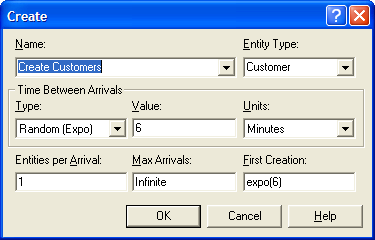
\includegraphics[width=0.6\linewidth,height=0.6\textheight]{./figures2/ch2/fig29PMCreateModule} 

}

\caption{Pharmacy model CREATE module}\label{fig:PMCreateModule}
\end{figure}

Make sure that you specify the units for time as minutes and be sure to
press OK; otherwise, your work within the module will be lost. In
addition, as you build models you never know what could go wrong;
therefore, you should save your models often as you proceed through the
model building process. Take the opportunity to save your model before
proceeding.

Before proceeding there is one last thing that you should do related to
the entities. Since the customers drive cars, you will change the
picture associated with the customer entity that was defined in the
CREATE module. To do this you will use the ENTITY module within the
Basic Process panel. The ENTITY module is a data module. A data module
cannot be dragged and dropped into the model window. Data modules
require the model builder to enter information in either the spreadsheet
window or in a dialog box. To see the dialog box, select the row from
the spreadsheet view, right-click and choose the edit via dialog option.
You will use the spreadsheet view here. Select the ENTITY module in the
Basic Process panel and use the corresponding spreadsheet view to select
the picture for the entity as shown in
Figure~\ref{fig:PMEntityModule}.

\begin{figure}

{\centering 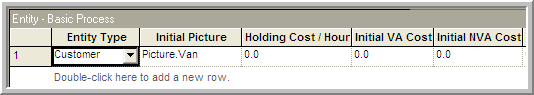
\includegraphics[width=0.8\linewidth,height=0.8\textheight]{./figures2/ch2/fig30PMEntityModule} 

}

\caption{Pharmacy model ENTITY module}\label{fig:PMEntityModule}
\end{figure}

\hypertarget{ch2:PM:Resources}{%
\subsection{Specifying the Resources}\label{ch2:PM:Resources}}

Go to the Basic Process Panel and select the RESOURCE module. This
module is also a data module. As you selected the RESOURCE module, the
data sheet window (Figure \ref{fig:PMResourceDM}) should have changed to reflect this selection.
Double-click on the row in the spreadsheet module for the RESOURCE
module to add a resource to the model.

\begin{figure}

{\centering 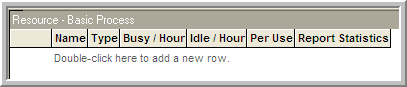
\includegraphics[width=0.75\linewidth,height=0.75\textheight]{./figures2/ch2/fig31PMResourceDM} 

}

\caption{RESOURCE module in data sheet view}\label{fig:PMResourceDM}
\end{figure}

After the resource row has been added, select the row and right-click.
This will bring up a context menu. From this context menu, select edit
via dialog box. Make the resulting dialog box look like
Figure~\ref{fig:PMResourceDB} You can also type in the same
information that you typed in the dialog box from within the spreadsheet
view. This defines a resource that can be used in the model. The
resource's name is Pharmacist and it has a capacity of one. Now, you
have to indicate how the customers will use this resource within a
process.

\begin{figure}

{\centering 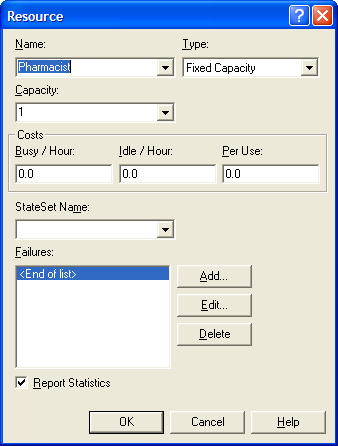
\includegraphics[width=0.45\linewidth,height=0.45\textheight]{./figures2/ch2/fig32PMResourceDialog} 

}

\caption{RESOURCE dialog box}\label{fig:PMResourceDB}
\end{figure}

\hypertarget{ch2:PM:Process}{%
\subsection{Specify the Process}\label{ch2:PM:Process}}

A process can be thought of as a set of activities experienced by an
entity. There are two basic ways in which processing can occur: resource
constrained and resource unconstrained. In the current situation,
because there is only one pharmacist and the customer will need to wait
if the pharmacist is busy, the situation is resource constrained. A
PROCESS module provides for the basic modeling of processes within an
model. You specify this within a PROCESS module by having the entity
\emph{seize} the resource for the specified usage time. After the usage time
has elapsed, you specify that the resource is \emph{released}. The basic
pseudo-code can now be modified to capture this concept as illustrated
in the following pseudo-code.

\begin{verbatim}
CREATE customers with EXPO(6) time between arrivals
SEIZE 1 pharmacist 
DELAY for EXPO(3) minutes 
RELEASE 1 pharmacist
DISPOSE customer
\end{verbatim}

Open up the PROCESS module and fill it out as indicated in
Figure~\protect\hyperlink{fig:ch4ProcessModule}{1.23}. Change the ``Action'' drop down dialog
box to the (Seize, Delay, Release) option. Use the ``Add'' button within the
``Resources'' area to indicate which resources the customer will use. In
the pop up Resources dialog, indicate the name of the resource and the
number of units desired by the customer. Within the ``Delay Type'' area,
choose Expression as the type of delay and type in expo(3) as the
expression. This indicates that the delay, which represents the service
time, will be randomly distributed according to an exponential
distribution with a mean of 3 minutes. Make sure to change the units
accordingly. When a PROCESS module uses the (Seize, Delay, Release) option, Arena automatically translates this to individual SEIZE, DELAY, and RELEASE modules, just like outlined in the pseudo-code. These modules (SEIZE, DELAY, RELEASE) are executed individually as the entities experience the process. It is very useful to understand what happens when these modules are executed.

\begin{figure}

{\centering 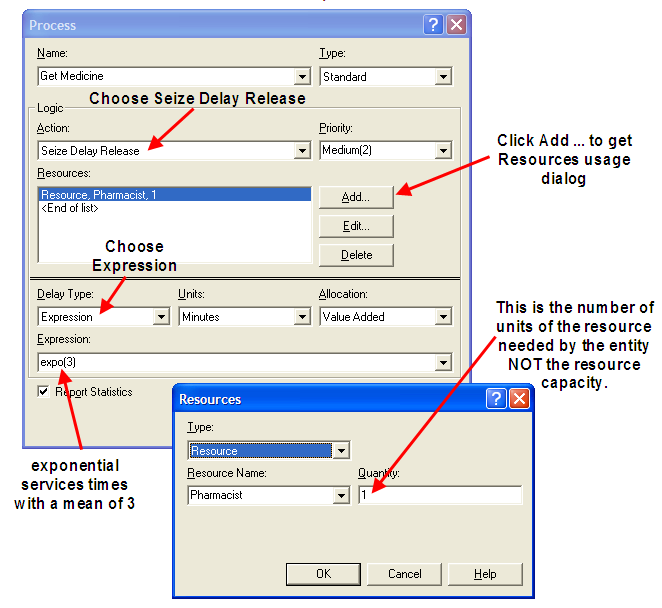
\includegraphics[width=0.65\linewidth,height=0.65\textheight]{./figures2/ch2/fig34PMProcessModule} 

}

\caption{PROCESS module seize, delay, release option}\label{fig:PMProcessModule}
\end{figure}

When an entity seizes a resource, the number of units available of the resource's capacity is (automatically) checked against the amount of units requested by the entity. There is a global variable (function) defined for each resource called, NR(\texttt{Resource\ ID}), that returns the number of units of the resource that have been allocated to entity requests. For example, suppose a resource called, \texttt{rBankTeller}, has \emph{capacity}, 3, and one of the 3 units (tellers) has already been allocated to a customer for use. That is, one of the tellers is currently serving a customer. In this case, NR(\texttt{rBankTeller}), will have the value 1. There is also a global variable (function) called MR(\texttt{Resource\ ID}) that holds the number of units of capacity defined for the resource. In this example, MR(\texttt{rBankTeller}) has the value 3. In the drive through pharmacy example the value of MR() is 1. Again, MR() holds the current \emph{capacity} of the resource. Obviously, resources can have capacity value of various amounts.

The number of available units of the resource is always the difference, MR(\texttt{Resource\ ID}) - NR(\texttt{Resource\ ID}). In this bank example, the value of MR(\texttt{rBankTeller}) - NR(\texttt{rBankTeller}) is currently 2 (3 - 1 = 2) because a customer is in service. Thus, an arriving customer that wants one teller will not have to wait in the queue associated with the SEIZE module and will be immediately allocated one of the available tellers. The value of NR(\texttt{rBankTeller}) will be incremented by 1 unit and the number of available units, MR(\texttt{rBankTeller}) - NR(\texttt{rBankTeller}), will decrease by 1. If an entity requests more than the current number of available units of the resource, the entity will be \emph{automatically} placed in the queue associated with the SEIZE module.

The units of a resource that have been allocated to an entity by a successful SEIZE will remain allocated to that entity until those units are released via a RELEASE module. An entity can release 1 or more units of the allocated resource when executing a RELEASE module. When an entity executes a RELEASE module the allocated units of the resource are given back to the resource and NR(\texttt{Resource\ ID}) is \emph{decremented} by the amount released. When the units of the resource are released, the queue associated with the seize (with the highest seize priority) is checked to see if any entities are waiting and if so, those entities are processed to check if their number of units requested of the resource can be allocated. The processing of the queue is based on the queue processing rule (e.g.~FIFO (first in, first out), LIFO (last in, first out), random, and priority ranking).

Suppose that a resource has capacity of 1 unit. If there are 2 processes
(or seizes) that seize the same resource and entities are waiting in
separate queues, the entity that activated the seize with the highest
priority will get the resource first. If both seize requests have the
same priority, then the entity that activated its seize first will go
first (first come first served). The priority field for the seize
controls the priority of the seize. It can be anything that evaluates to
a number. A resource is considered busy if \emph{at least 1 unit} of its
capacity has been allocated. A resource is considered idle when \emph{all}
units are idle and the resource is not failed or inactive. The failed and inactive states of resources are discussed in Section \ref{ch6:AdvResModeling}.

\begin{rmdnote}
A common misunderstanding by novice modelers is to think that they must continually check MR(\texttt{Resource\ ID}) - NR(\texttt{Resource\ ID}) to see if the resource is available. Do not think this way. The purpose of the SEIZE and RELEASE constructs is to manage the allocation and deallocation of resource units. While there can be legitimate reasons for using the values of NR(\texttt{Resource\ ID}) and MR(\texttt{Resource\ ID}) within a model, you should not make the mistake of polling resources for availability. The resource allocation process is done automatically using SEIZE and RELEASE. If you do not like how the resource units are being allocated, then you should use more advanced concepts as discussed in Chapter \ref{ch6}.
\end{rmdnote}

Now we are ready to specify how to execute the pharmacy model.

\FloatBarrier

\hypertarget{ch2:PM:RunParameters}{%
\subsection{Specify Run Parameters}\label{ch2:PM:RunParameters}}

Let's assume that the pharmacy is open 24 hours a day, 7 days a week. In
other words, it is always open. In addition, assume that the arrival
process does not vary with respect to time. Finally, assume that
management is interested in understanding the long term behavior of this
system in terms of the average waiting time of customers, the average
number of customers, and the utilization of the pharmacist. This kind of simulation is called an infinite horizon simulation and will be discussed in more detail in Chapter \ref{ch5}.

To simulate this situation over time, you must specify how long to run
the model. Ideally, since management is interested in long run
performance, you should run the model for an infinite amount of time to
get long term performance; however, you probably don't want to wait that
long! For the sake of simplicity, assume that 10,000 hours of operation
is long enough. Within the environment, go to the Run menu item and
choose Setup. After the Setup dialog box appears, select the Replication
parameters tab and fill it out as shown in
Figure \ref{fig:PMRunParameters}. The \emph{Replication Length} text box
specifies how long the simulation will run. Notice that the base time
units were changed to minutes. This ensures that information reported by
the model is converted to minutes in the output reports.

\begin{figure}

{\centering 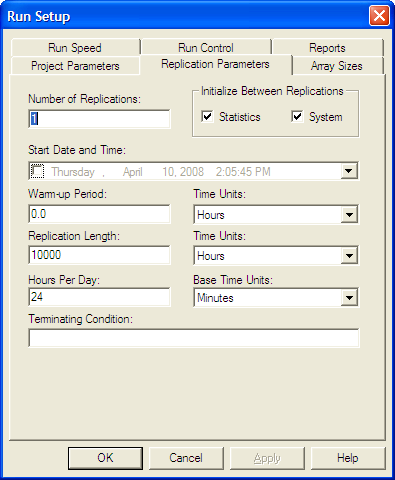
\includegraphics[width=0.6\linewidth,height=0.6\textheight]{./figures2/ch2/fig35PMRunParameters} 

}

\caption{Run setup replication parameters tab}\label{fig:PMRunParameters}
\end{figure}

The fully completed model is available within this chapter's files as file, \emph{PharmacyModel.doe}.

Now, the model is ready to be executed. You can use the Run menu to do
this or you can use the convenient "VCR" like run toolbar (Figure \ref{fig:PMRunToolbar}). The Run
button causes the simulation to run until the stopping condition is met.
The Fast Forward button runs the simulation without animation until the
stopping condition is met. The Pause button suspends the simulation run.
The Start Over button stops the run and starts the simulation again. The
Stop button causes the simulation to stop. The animation slider causes
the animation to slow down (to the left) or speed up (to the right).

\begin{figure}

{\centering 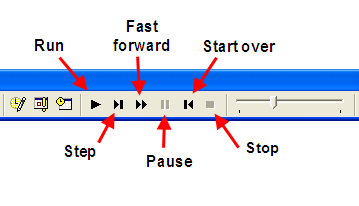
\includegraphics[width=0.5\linewidth,height=0.5\textheight]{./figures2/ch2/fig36PMRunToolbar} 

}

\caption{Run toolbar}\label{fig:PMRunToolbar}
\end{figure}

\begin{figure}

{\centering 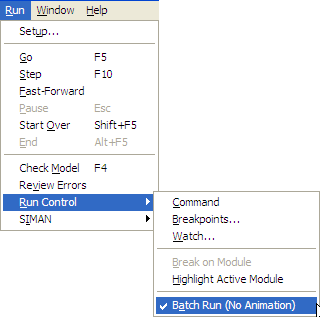
\includegraphics[width=0.45\linewidth,height=0.45\textheight]{./figures2/ch2/fig37PMBatchRun} 

}

\caption{Batch run no animation option}\label{fig:PMBatchRun}
\end{figure}

When you run the model, you will see the animation related to the
customers waiting in line. Because the length of this run is very long,
you should use the fast forward button on the "VCR" run toolbar to
execute the model to completion without the animation. Instead of using
the fast forward button, you can significantly speed up the execution of
your model by running the model in batch mode without animation. To do
this, you can use the Run menu as shown in
Figure~\ref{fig:PMBatchRun} and then when you use the VCR Run button
the model will run much faster without animation.

\FloatBarrier

\hypertarget{ch2:PM:Results}{%
\subsection{Analyze the Results}\label{ch2:PM:Results}}

After running the model, you will see a dialog (Figure \ref{fig:PMRunCompletion}) indicating that the
simulation run is completed and that the simulation results are ready.
Answer yes to open up the report viewer.

\begin{figure}

{\centering 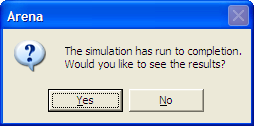
\includegraphics[width=0.35\linewidth,height=0.35\textheight]{./figures2/ch2/fig38PMRunCompletion} 

}

\caption{Run completion dialog}\label{fig:PMRunCompletion}
\end{figure}

\begin{figure}

{\centering 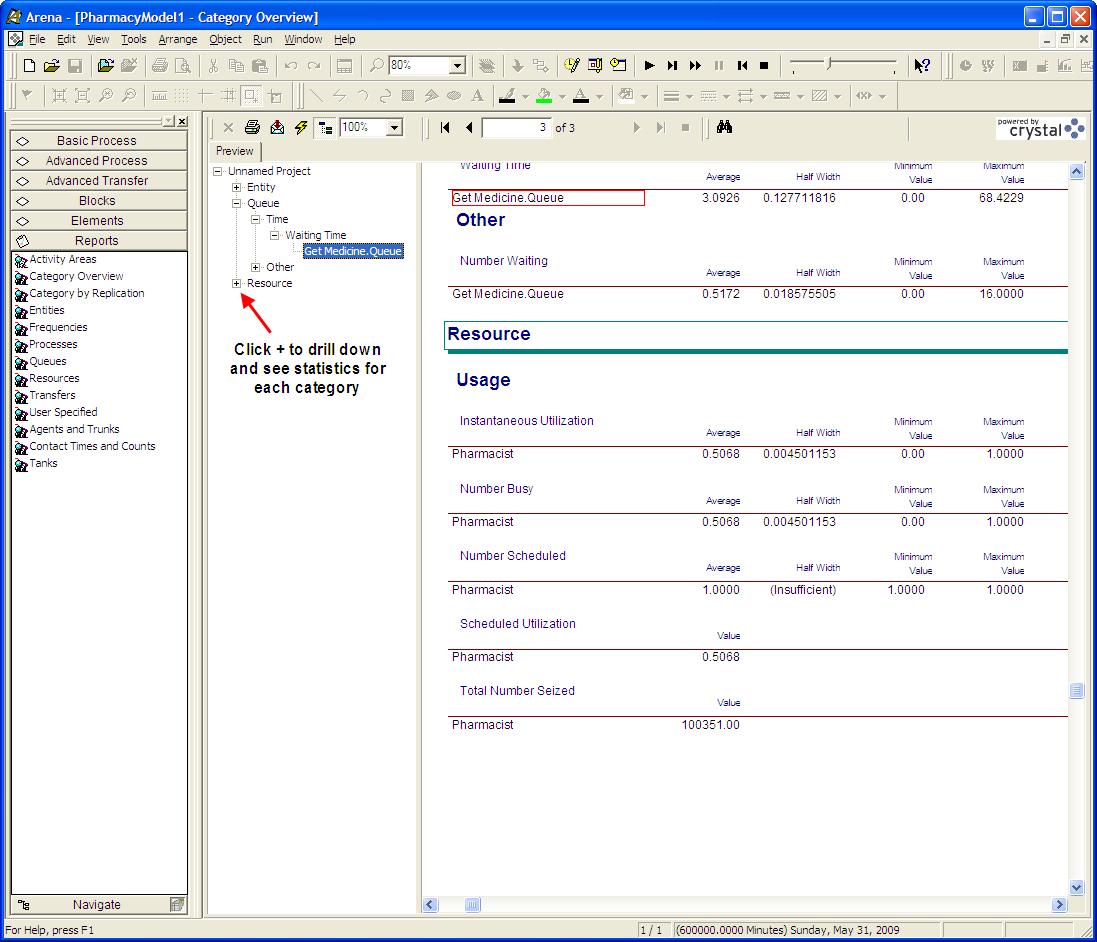
\includegraphics[width=0.9\linewidth,height=0.9\textheight]{./figures2/ch2/fig39PMResults} 

}

\caption{Results for pharmacy model}\label{fig:PMResults}
\end{figure}

In the reports preview area, you can drill down to see the statistics
that you need. Go ahead and do this so that you have the report window
as indicated in Figure~\ref{fig:PMResults}. The reports indicate that customers wait
about 3 minutes on average in the line. reports the average of the
waiting times in the queue as well as the associated 95\% confidence
interval half-width. In addition, reports the minimum and maximum of the
observed values. These results indicate that the maximum a customer
waited to get service was 16 minutes. The utilization of the pharmacist
is about 50\%. This means that about 50\% of the time the pharmacist was
busy. For this type of system, this is probably not a bad utilization,
considering that the pharmacist probably has other in-store duties. The
reports also indicate that there was less than one customer on average
waiting for service. Using the Reports panel in the Project Bar you can
also select specific reports.

also produces a text-based version of these reports in the directory
associated with the model. Within the Windows File Explorer, select the
\emph{modelname.out} file, see
Figure~\protect\hyperlink{fig:ch4Files}{1.30}. This file can be read with any text editor
such as Notepad, see Figure \ref{fig:PMTextResults}.

\begin{figure}

{\centering 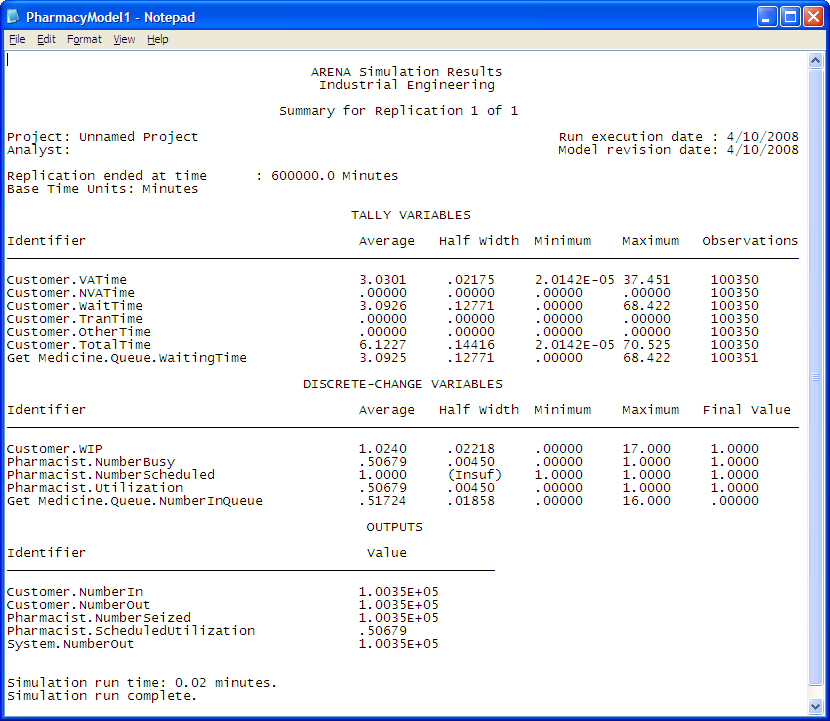
\includegraphics[width=0.9\linewidth,height=0.9\textheight]{./figures2/ch2/fig41PMTextResults} 

}

\caption{Text file summary results}\label{fig:PMTextResults}
\end{figure}

Also as indicated in Figure \ref{fig:PMWindowsExplorer}, Arena generates additional files when you run the
model. The \emph{modelname.accdb} file is a Microsoft Access database that
holds the information displayed by the report writer. The \emph{modelname.p}
file is generated when the model is checked or run. If you have errors
or warnings when you check your model, the error file will also show up
in the directory of your \emph{modelname.doe} file

\begin{figure}

{\centering 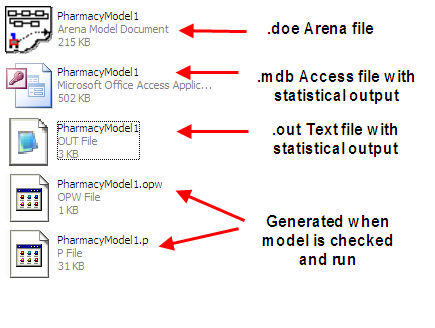
\includegraphics[width=0.6\linewidth,height=0.6\textheight]{./figures2/ch2/fig40PMWidowsExplorer} 

}

\caption{Files generated when running Arena}\label{fig:PMWindowsExplorer}
\end{figure}

This single server waiting line system is a very common situation in
practice. In fact, this exact situation has been studied mathematically
through a branch of operations research called queuing theory. As will
be covered in Appendix \ref{app:qtAndInvT} for specific modeling situations, formulas for the
long term performance of queuing systems can be derived. This particular
pharmacy model happens to be an example of an M/M/1 queuing model. The
first M stands for Markov arrivals, the second M stands for Markov
service times, and the 1 represents a single server. Markov was a famous
mathematician who examined the exponential distribution and its
properties. According to queuing theory, the expected number of customer
in queue, \(L_q\), for the M/M/1 model is:

\begin{equation}
\begin{aligned}
L_q & = \dfrac{\rho^2}{1 - \rho} \\
\rho & = \lambda/\mu \\
\lambda & = \text{arrival rate to queue} \\
\mu & = \text{service rate}
\end{aligned}
\label{eq:mm1}
\end{equation}

In addition, the expected waiting time in queue is given by
\(W_q = L_q/\lambda\). In the pharmacy model, \(\lambda\) = 1/6, i.e.~1
customer every 6 minutes on average, and \(\mu\) = 1/3, i.e.~1 customer
every 3 minutes on average. The quantity, \(\rho\), is called the
utilization of the server. Using these values in the formulas for \(L_q\)
and \(W_q\) results in:

\[
\begin{aligned}
\rho & = 0.5 \\
L_q  & = \dfrac{0.5 \times 0.5}{1 - 0.5} = 0.5  \\
W_q & = \dfrac{0.5}{1/6} = 3 \: \text{minutes}
\end{aligned}
\]

In comparing these analytical results with the simulation results, you
can see that they match to within statistical error. Later in this text,
the analytical treatment of queues and the simulation of queues will be
developed. These analytical results are available for this special case
because the arrival and service distributions are exponential; however,
simple analytical results are not available for many common
distributions, e.g.~lognormal. With simulation, you can easily estimate
the above quantities as well as many other performance measures of
interest for wide ranging queuing situations. For example, through
simulation you can easily estimate the chance that there are 3 or more
cars waiting.

\hypertarget{ch2:PM:Extension}{%
\section{Extending the Drive Through Pharmacy Model}\label{ch2:PM:Extension}}

The drive through pharmacy model presents a very simple process for the
customer: enter, get served, and depart. To make the model a little more
realistic consider that a customer my decide not to wait in line if
there is a long line of waiting customers. Let's assume that if there
are four or more customers in the line when a customer arrives that they
decide to go to different pharmacy. To model this situation we need to
be able to direct the customer along different paths in the model. This
can be accomplished using the DECIDE module. The DECIDE module shown in
Figure \ref{fig:PMDecideSymbol} has one input port and possibly two or more
output ports. Thus, an entity that enters in the input port side of the
DECIDE module can take different paths out of the module. The path can
be chosen based on a condition or set of conditions, or based on a
probability distribution.

\begin{figure}

{\centering 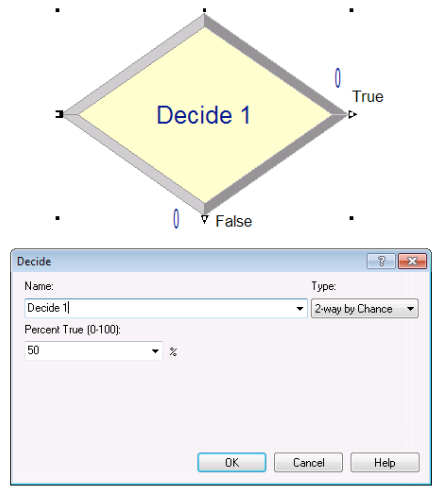
\includegraphics[width=0.4\linewidth,height=0.4\textheight]{./figures2/ch2/fig42PMDecideSymbol} 

}

\caption{DECIDE flowchart symbol and module dialog}\label{fig:PMDecideSymbol}
\end{figure}

To model the situation that an arriving pharmacy customer may decide to
go to a different pharmacy, we need to use a condition within the DECIDE
module. The decision to go to a different pharmacy depends upon how many
customers are in the waiting line. Thus, we need a method to determine
how many customers are in the pharmacy queue at any time. This can be
accomplished using the \texttt{NQ(queue\ name)} function. The \texttt{NQ(queue\ name)}
function returns the number of entities being held in the named queue.
In the model, the queue that holds the customers is call \emph{Get
Medicine.Queue}. The name of the queue for a PROCESS module takes on the
name of the PROCESS module with the word Queue appended. Therefore, the
following condition can be used to test whether or not the arriving
customer should go somewhere else is: \texttt{NQ(Get\ Medicine.Queue)\ \textless{}=\ 3}.
The following pseudo-code illustrates these ideas.

\begin{verbatim}
CREATE customers with EXPO(6) time between arrivals
DECIDE IF NQ(Get Medicine.Queue) <= 3 customers
SEIZE 1 pharmacist 
DELAY for EXPO(3) minutes 
RELEASE 1 pharmacist 
DISPOSE customer
\end{verbatim}

Based on this pseudo-code, the customer only enters the PROCESS module
if there are 3 or less cars waiting in line. The overall model is
illustrated in Figure \ref{fig:PMExtensionOverview}. Notice that there are now two
DISPOSE modules, one for customers who do not enter (balk) and one for
those that enter and complete service.
Figure \ref{fig:PMDecideModule} shows the use of the \texttt{NQ()} function
to chose the correct path.

\begin{figure}

{\centering \includegraphics[width=0.85\linewidth,height=0.85\textheight]{./figures2/ch2/fig43PMWithDecideOverview} 

}

\caption{Overview of pharmacy model with DECIDE module}\label{fig:PMExtensionOverview}
\end{figure}

\begin{figure}

{\centering \includegraphics[width=0.6\linewidth,height=0.6\textheight]{./figures2/ch2/fig44PMDecideModule} 

}

\caption{DECIDE module dialog with condition specified}\label{fig:PMDecideModule}
\end{figure}

Running the model using the same conditions as before results less
waiting and utilization as show in Figure \ref{fig:PMDecideResults}. This is because less customers
enter the system. In the next chapter, we will learn how to quantify the
probability of losing customers due to long lines.

\begin{figure}

{\centering \includegraphics[width=0.6\linewidth,height=0.6\textheight]{./figures2/ch2/fig45PMDecideResults} 

}

\caption{Results for pharmacy model with DECIDE module}\label{fig:PMDecideResults}
\end{figure}

\FloatBarrier

\hypertarget{ch2:PM:Animate}{%
\section{Animating the Drive Through Pharmacy Model}\label{ch2:PM:Animate}}

While running the pharmacy model with the animation on, you saw some of
Arena's basic animation capabilities. Positioned over the PROCESS module
is an animation queue, which shows the cars that are waiting for the
pharmacist. has many other animation features that can be added to a
model. Animation is important for helping to verify that the model is
working as intended and for validating the model's representation of the
real system. This section will illustrate a few of Arena's simpler
animation features by having you augment the basic pharmacy model. In
particular, you will change the entity picture from a van to a car, draw
the pharmacy building, and show the state of the pharmacist (idle or
busy). You will also animate the number of cars waiting in the line
(both visually and numerically).

When defining the entity type, a picture of a van was originally
selected for the entity. has a number of other predefined graphical
pictures that can be used within the model. The available entity
pictures can be found from the Edit menu as shown in
Figure \ref{fig:PMAEntityPictures}. You can select different picture files by navigating to where they are installed within your Arena installation. See Figure \ref{fig:PMAEntityPictFolder} This may vary by installation. For example, the picture library can be found at the following location in my installation \texttt{C:\textbackslash{}Users\textbackslash{}Public\textbackslash{}Documents\textbackslash{}Rockwell\ Software\textbackslash{}Arena\textbackslash{}PictureLibraries}.

\begin{figure}

{\centering \includegraphics[width=0.35\linewidth,height=0.35\textheight]{./figures2/ch2/fig46PMAEntityPictures} 

}

\caption{Accessing entity pictures}\label{fig:PMAEntityPictures}
\end{figure}

\begin{figure}

{\centering \includegraphics[width=0.6\linewidth,height=0.6\textheight]{./figures2/ch2/fig47PMAEntityPictFolder} 

}

\caption{Entity pictures folder}\label{fig:PMAEntityPictFolder}
\end{figure}

Once you have selected Edit \(>\) Entity Pictures, you should see the
entity picture placement dialog as shown in
Figure \ref{fig:PMAPictPlacement}. The entity picture placement
dialog is divided into two functions: the picture list (on the left of
dialog) and the picture library (on the right of the dialog). The
picture list represents the entity pictures that are listed in the
ENTITY module. If you scroll down you will find the picture of the van
in the list. By navigating to the picture libraries within the
distribution folder on your hard-drive (see Figure \ref{fig:PMAEntityPictFolder} you can select the \emph{Vehicles.plb}
file. When selected as the current library, your entity picture
placement dialog should look as shown in Figure \ref{fig:PMAPictPlacement}.

\begin{figure}

{\centering \includegraphics[width=0.8\linewidth,height=0.8\textheight]{./figures2/ch2/fig48PMAPicturePlacement} 

}

\caption{Entity picture placement dialog}\label{fig:PMAPictPlacement}
\end{figure}

Scroll down in the vehicle library and select the red car, then select
the ``\(<<\)'' button to move the picture to the picture list. Finally, you
should give the picture a name in the list (e.g.~Red Car). Now, go back
to the ENTITY module and associate the picture with your entity. At the
time of this writing, the name does not appear on the Entity module drop
down list, but the picture is available. Just type in the correct name
in the Entity module to have the entity picture represented by the red
car.

Now, you will use Arena's drawing tools to draw the outline of the
pharmacy building. has standard drawing tools (e.g.~lines, rectangles,
polygons, etc) as well as way to add text, fill options etc. These tools
are available through the Drawing toolbar as shown in
Figure \ref{fig:PMADrawingToolbar}. You can also turn on the drawing grid and
the ruler, which are useful in placing the drawing objects. In this
situation, drawing will be kept to a rather simple/crude representation
of the pharmacy. Essentially, the pharmacy will be represented as a box,
the drive through lane as a line with the road line pattern, and the
pass through service window as two lines with 3pt thickness.

\begin{figure}

{\centering \includegraphics[width=0.8\linewidth,height=0.8\textheight]{./figures2/ch2/fig49PMADrawingToolbar} 

}

\caption{Basic drawing toolbar}\label{fig:PMADrawingToolbar}
\end{figure}

Figure \ref{fig:PMASimpleDrawing} illustrates the background drawing for
the pharmacy. The drawing editor works like most computer based drawing
editors. You should just drag and drop the items, set the fill options,
thickness, and line pattern as you go. This portion of this example is
available in the \emph{PharmacyModelWithAnimationS1.doe} file.

\begin{figure}

{\centering \includegraphics[width=0.9\linewidth,height=0.9\textheight]{./figures2/ch2/fig50PMASimpleDrawing} 

}

\caption{Simple pharmacy drawing within Arena model Window}\label{fig:PMASimpleDrawing}
\end{figure}

In the next part of the example, you will animate the resource so that
you can see when the pharmacist is busy or idle, provide a location to
show the customer currently being served, and better represent the
waiting cars in the drawing.

Within a resource can be in one of four default states (idle, busy,
inactive, and failed). The inactive and failed states will be discussed
later in the text. The idle state represents the situation that at least
1 unit of the resource is available. In the pharmacy model, there is
only 1 pharmacist, so if the pharmacist is not serving the customer, the
pharmacist is considered idle. The busy state represents the situation
where all available units of the resource are currently seized. In the
case of the pharmacy model, since there is only 1 resource unit (the
pharmacist), the resource is busy when the sole pharmacist is seized. In
the animation, you will visibly represent the state of the pharmacist.
This can be done through Arena's animate toolbar and in particular the
animate resource button.

\begin{enumerate}
\def\labelenumi{\arabic{enumi}.}
\item
  Click the Resource button on the Animate toolbar.
\item
  The Resource Placement dialog box appears. Use the open button to
  navigate to the \emph{people.plb} picture library.
\item
  Select the over head person view picture from the library's list of
  pictures, see Figure \ref{fig:PMAResourceAnimation} Then, select the Copy button.
  This will cause a copy of the picture to be made in the library.
\item
  After copying the picture, double-click on the picture. This will
  put you in the resource editor. This is like a drawing editor. For
  simplicity, just select the picture and change the fill color to
  green. If you want to make it look just like the picture in the
  text, you need to un-group the picture elements and change their
  appearance as necessary.
\item
  Assign the white over head person view picture to the idle state and
  the green picture that was just made to the busy state. To change
  the idle picture: Click the Idle button in the table on the left.
  Select from the picture library table on the right the picture of
  the white over head view person picture. Click the Transfer button
  between the tables to use the picture for the Idle resource state.
  To change the busy picture: Click the Busy button in the table on
  the left. Select from the picture library table on the right the
  picture of green worker that was just made. Click the Transfer
  button between the tables to use the selected picture when the
  pharmacist is busy.
\item
  Now you need to rotate the picture so that the person is facing
  down. Double-click on the new Idle resource picture to open the
  resource editor. Then, you should select the whole picture and
  choose Arrange \(>\) Rotate in order to rotate the picture so that the
  pharmacist is facing down. Close the editor and do this for the Busy
  state also.
\item
  Click on the Seize Area check box. This will be discussed shortly.
\item
  Click OK to close the dialog box. (All other fields can be left with
  their default values.) will ask about whether you want to save the
  changes to picture library. If you want to keep the green over head
  view person for use in later models, answer yes during the saving
  process. The cursor will appear as a cross hair. Move it to the
  model window and click to place the pharmacist resource animation
  picture within the pharmacy.
\end{enumerate}

Now that the pharmacist is placed in the pharmacy, it would be nice to
show the pharmacist serving the current customer. This can be done by
using the seize area for a resource. The seize area animates the
entities that have seized the resource. By default the seize area is not
shown on the animation of a resource. The checking of the Seize Area
check box allows the seize area to be visible. After placing the
resource, zoom in on the resource and notice a small double circle. This
is the seize area. Select the seize area and drag it so that it is
positioned in the road adjacent to the pharmacy.

Now, you need to place the queue of waiting cars on the road. Select the animation queue on top
of the Get Medicine PROCESS module and delete it. Now, go to the Queue
button on the Animate toolbar and select it. This will allow you to
create a new queue animation element that is not physically attached to
the Get Medicine PROCESS module and place it in the road. Fill in the
Queue animation dialog as shown in Figure \ref{fig:PMAQueueAnimation}. Once you press OK, the cursor will
turn in to a cross-hair and allow you to place the animation queue.

\begin{figure}

{\centering \includegraphics[width=0.8\linewidth,height=0.8\textheight]{./figures2/ch2/fig51PMAResourceAnimation} 

}

\caption{Resource animation state picture assignment}\label{fig:PMAResourceAnimation}
\end{figure}

\begin{figure}

{\centering \includegraphics[width=0.5\linewidth,height=0.5\textheight]{./figures2/ch2/fig52PMAQueueAnimation} 

}

\caption{Queue animation dialog}\label{fig:PMAQueueAnimation}
\end{figure}

The final piece of animation that you will perform is to show the
current number of waiting cars within the pharmacy. Select the Variable
button on the Animate toolbar and fill out the resulting dialog as per
Figure \ref{fig:PMAVariableAnimation}. The cursor should turn to
cross-hairs and you should place the variable animation inside the
pharmacy as shown in Figure \ref{fig:PMAFinalAnimation}.

\begin{figure}

{\centering \includegraphics[width=0.45\linewidth,height=0.45\textheight]{./figures2/ch2/fig53PMAVariableAnimation} 

}

\caption{Variable animation dialog}\label{fig:PMAVariableAnimation}
\end{figure}

\begin{figure}

{\centering \includegraphics[width=0.9\linewidth,height=0.9\textheight]{./figures2/ch2/fig54PMAFinalAnimation} 

}

\caption{Final animation for pharmacy example}\label{fig:PMAFinalAnimation}
\end{figure}

The last thing to do before running the animation will be to turn off
the animation associated with the flow chart connectors. This will stop
the animation of the customers within the flow chart modules and be less
of a distraction. The Object menu contains the option to disable/enable
the animation of the connectors as shown in Figure \ref{fig:PMADisablingConnector}.

\begin{figure}

{\centering \includegraphics[width=0.4\linewidth,height=0.4\textheight]{./figures2/ch2/fig55PMADisableConnectorAnimation} 

}

\caption{Disabling connector animation}\label{fig:PMADisablingConnector}
\end{figure}

The final version of the animated pharmacy model is available in the
file, \emph{PharmacyModleWithAnimationS2.doe}. If you run the model with the
animation on, you will see the pharmacist indicated as busy or idle, the
car currently in service, any cars lined up waiting, and the current
number of cars waiting as part of the animation.

\begin{rmdnote}
\textbf{How can I animate a resource that has capacity \textgreater{} 1}
This question is commonly asked because you want to show each unit of
the resource being busy. Unfortunately, this isn not easy to do because a
resource is considered busy if at least 1 unit of its capacity is busy. You
could animate the \texttt{NR(resource\ name)} variable, see Section \ref{ch6:AdvResModeling}, to show how many are busy (either numerically or with a level animation). Also, by showing the
seize point and adding multiple points you can show each entity as it is
using the resource. There is also something called a storage, see Section \ref{ch4:RevisedJFE:NewModules}, which will do just about the same thing. You can also animate 1-D variable by
having the variable indicate whether each unit is busy or not. All of
these methods are illustrated in the attached Arena model. This should
approximate what you are trying to do. The variable method is probably
the best but takes the most work. If you are going to use the variable
method, then you might just look at using a resource set instead. If you
want to use a resource animation and show each separately, then you need
to define a different resource to represent each unit of the overall
resource, put them in a set and seize/delay/release from the set. Then,
you can animate each of the individual resources in the standard manner. Please see the Arena file, \emph{ResourceAnimations.doe} that accompanies this chapter's files for an example.
\end{rmdnote}

Animation is an important part of the simulation process. It is
extremely useful for showing to decision makers and experts to explain
and ensure that the model is accepted. With this example, you have
actually learned a great deal about animating a model. One of the
standard practices is to rely on the default animation that is available
with the flow chart modules. Then, when animation is important for
validation and for convincing decision makers, the simulation analyst
can devote time to making the animation more worthy. Often, the
animation is developed in one area of the model which can be easily
accessed via the Navigate bar. Many detailed examples of what is
possible with animation come as demo models with the distribution. For
example, you should explore the models in the Examples folder (e.g.
\emph{FlexibleManufacturing.doe}). If you find that the drawing tools are
limiting, then you can use other drawing programs to make the
drawings and import them as background for your model. Arena also has the
capability for developing 3D animation; however, this is not discussed
in this text.

The first part of this text primarily uses the default animation that
comes with the placement of flow chart modules and concentrates on the
analysis of simulation models; however, Chapter \ref{ch7} returns to
more on the topic of animation, when material handling constructs (e.g.
conveyors and transporters) are examined.

\hypertarget{ch2:AttVariablesIO}{%
\section{Attributes, Variables, and Some I/O}\label{ch2:AttVariablesIO}}

In this section, we will dig deeper into the concepts of attributes and
variables. In addition, an introduction to some additional statistical collection will be discussed. Finally, we will see how to write data to a
file. To illustrate these concepts, we will expand upon the pharmacy model.

\hypertarget{ch2:ModifiedPharmacyModel}{%
\subsection{Modifying the Pharmacy Model}\label{ch2:ModifiedPharmacyModel}}

Suppose that customers who arrive to the pharmacy have either 1, 2, or 3
prescriptions to be filled. There is a 50\% chance that they have 1
prescription to fill, a 30\% chance that they have 2 prescriptions to
fill, and a 20\% chance that they have 3 prescriptions to fill. The time
to service a customer is still exponentially distributed but the mean
varies according to how many prescriptions that they need filled as shown
in Table \ref{tab:PresData}.

\hypertarget{tab:PresData}{}
\begin{longtable}[]{@{}lcc@{}}
\caption{\label{tab:PresData} Prescription related data}\tabularnewline
\toprule
\# Prescription & Chance & Service Time Mean\tabularnewline
\midrule
\endfirsthead
\toprule
\# Prescription & Chance & Service Time Mean\tabularnewline
\midrule
\endhead
1 & 50\% & 3 minutes\tabularnewline
2 & 30\% & 4 minutes\tabularnewline
3 & 20\% & 5 minutes\tabularnewline
\bottomrule
\end{longtable}

For illustrative purposes, current number of customers having 1, 2, or 3
prescriptions in system is needed within the animation of the model. In
addition, the total number of prescriptions in the system should also be
displayed. Statistics should be collected on the average number of
prescriptions in the system and on the average time a customer spends in
the system. For diagnostic purposes, the following information should be
captured to a file:

\begin{itemize}
\item
  When a customer arrives: The current simulation time, the entity
  number (IDENT), the entity's serial number, the number of
  prescriptions for the customer
\item
  When a customer departs: The current simulation time, the entity
  number (IDENT), the entity's serial number, the number of
  prescriptions for the customer, and the time of arrival, and the
  total time spent in the system
\end{itemize}

In addition to the above information, each of the above two cases should
be denoted in the output. The simulation should be run for only 30
customers.

As we saw earlier in the chapter, you should follow a
basic modeling recipe and address the following steps:

\begin{itemize}
\item
  \emph{What is the system?}

  \begin{itemize}
  \item
    \emph{What are the elements of the system?}
  \item
    \emph{What information is known by the system?}
  \end{itemize}
\item
  \emph{What are the required performance measures?}
\item
  \emph{What are the entity types?}

  \begin{itemize}
  \item
    \emph{What information must be recorded or remembered for each entity
    instance?}
  \item
    \emph{How are entities (entity instances) introduced into the
    system?}
  \end{itemize}
\item
  \emph{What are the resources that are used by the entity types?}

  \begin{itemize}
  \tightlist
  \item
    \emph{Which entity types use which resources and how?}
  \end{itemize}
\item
  \emph{What are the process flows? Sketch the process or make an activity
  flow diagram}
\item
  \emph{Develop pseudo-code for the situation}
\item
  \emph{Implement the model in Arena}
\end{itemize}

By considering each of these questions in turn, you should have a good
start in modeling the system.

In this example, the system is again the pharmacy and its waiting line.
The system knows about the chance for each prescription amount, the
inter-arrival time distribution, and the service time distributions with
their means by prescription amount. The system must also keep track of
how many prescriptions of each type are in the pharmacy and the total
number of prescriptions in the pharmacy. The performance of the system
will be measured by using the average number of prescriptions in the
system and the average time a customer spends in the system. As in the
previous model, the entity will be the customers. Each customer must
know the number of prescriptions needed. As before, each customer
requires a pharmacist to have their prescription filled. The activity
diagram will be exactly the same as shown in Figure \ref{fig:ActivityDiagram} because
the activity and use of resources of the customer has not changed.

When implementing this model, the following modules will be
used:

\begin{itemize}
\item
  CREATE This module will be used to create the 30 customers
\item
  ASSIGN This module will be used to assign values to variables and
  attributes.
\item
  READ/WRITE This module will be used to write out the necessary
  information from the customers.
\item
  PROCESS This module will be used to implement the prescription
  filling activity with the required pharmacist.
\item
  RECORD This module will be used to record statistics on the system
  time of the customers
\item
  DISPOSE This module will be used to dispose of the entities that
  were created.
\item
  FILE This data module defines the characteristics of the operating
  system file used by the READ/WRITE module.
\item
  VARIABLE This data module will be used to define variables to track
  the number of customers having the different amounts of
  prescriptions and to track the total number of prescriptions.
\item
  ATTRIBUTE This data module will be used to define attributes associated with the customer.
\end{itemize}

Thus, the new modules are the READ/WRITE module, the FILE module, and the RECORD module.

To start the modeling, the variables and attributes necessary for the
problem need to be understood. In the problem, the system needs to keep
track of the total number of prescriptions and the number of customers
that need 1, 2, or 3 prescriptions filled. Therefore, variables to keep
track of each of these items are required. A scalar variable can be used
to track the number of prescriptions (\texttt{vNumPrescriptions}) in the system
and a 1-D variable (\texttt{vNP}) with 3 elements can be used to track the
number of customers requiring each of the 3 prescription amounts.

In the example, each customer needs to know how many prescriptions that
he/she needs to have filled. Therefore, the number of prescriptions
(\texttt{myNP}) needs to be an entity attribute. In addition, the arrival time of
each customer and the customer's total time in the system must be
written out to a file. Thus, each entity representing a customer must
remember when it arrived to the pharmacy. Do real customers need to
remember this information? No! However, the \emph{modeling} requires this
information. Thus, attributes (and variables) can be additional
characteristics required by the modeler that are not necessarily part of
the real system. Thus, the arrival time (\texttt{myArriveTime}) of each
customer should be modeled as an entity attribute.

To understand why this information must be stored in an attribute
consider what would happen if you tried to use a variable to store the
number of prescriptions of the incoming customer. Entities move from one
block to another during the simulation. In general, entities may delay
their progress due to simulation logic. When this happens, other
entities are allowed to move. If the number of prescriptions for a specific
customer instance was stored in a (global) variable, then during the movement
cycle of the other entities (customers), some other entity instance might change the value
of the variable. Thus, the information concerning the current customer's
number of prescriptions would be over written by the next customer that
enters the system. Thus, this information must be carried with the
entity and not stored globally. Global variables are very useful for communicating information
between entities; however, as in any programming language care must be
taken to use them correctly.

\begin{rmdnote}
\textbf{What is the difference between attributes and variables?}
The key difference is that a variable is global. A variable
belongs to the system. Attributes are attached to an entity instance. Variables
define a place in memory in which data can be stored. Since the memory
is global to the model, any module or entity can read/write/use the
value of the variable. Memory allocated to an attribute is stored in the \emph{entity table} with the specific entity instance as discussed in Section \ref{ch2:EntitiesAttributesVariables}. If you have experience with a programming language like Java, then Arena variables are like static class variable, which is shared by all instances of the class. Arena attributes are like Java fields of the class, which are attached only to the object instances.
\end{rmdnote}

The information in Table \ref{tab:PresData} also needs to be modeled. Does this
information belong to the system or to each customer? While the
information is \emph{about} customers (in general), each customer does not need to "carry"
this information. The information is really about how to create the
customers. In other words, it is about the entity type not the entity instance. The system must know how to create the customers, thus this
information belongs to the system. The number of prescriptions per
customer can be modeled as a random variable with a discrete
distribution. The information about the mean of the service time
distributions can be kept in a 1-D variable with 3 elements representing
the mean of each distribution. The basic pseudo-code for this situation
is given in the following pseudo-code.

\begin{verbatim}
CREATE customers with EXPO(6) time between arrivals
BEGIN ASSIGN
  myNP = DISC(0.5, 1, 0.8, 2, 1.0, 3)
  vNumPrescriptions = vNumPrescriptions + myNP
  vNP(myNP) = vNP(myNP) + 1
  myArriveTime = TNOW  //TNOW represents the current simulation time
END ASSIGN
WRITE customer arrival information to a file
BEGIN PROCESS
  SEIZE 1 pharmacist
  DELAY for EXPO(3) minutes
  RELEASE 1 pharmacist
END PROCESS
RECORD (TNOW - myArriveTime)
WRITE customer departure information to a file
DISPOSE customer
\end{verbatim}

In what follows, the previously developed pharmacy model will be used as
a basis for making the necessary changes for this situation. If you want
to follow along with the construction of the model, then make a copy of
the pharmacy model of Section \ref{ch2:ModelingThePharmacy}. You should start by defining the variables for the example. With your copy of the model open, go to the Basic Panel and
select the VARIABLE data module and define the following variables:

\begin{itemize}
\item
  \texttt{vNumPrescriptions} This scalar variable should count the total
  number of prescriptions in the system. This variable should be
  initialized at the value 0.0.
\item
  \texttt{vNP} This 1-D variable should have 3 rows and should count the
  number of customers having 1, 2, 3 prescriptions currently in the
  system. The index into the array is the prescription quantity. Each
  element of this variable should be initialized at the value 0.0.
\item
  \texttt{vServiceMean} This 1-D variable should have 3 rows representing the
  mean of the service distributions for the 3 prescription quantities.
  The index into the array is the prescription quantity. The elements
  (1, 2, 3) of this variable should be initialized at the values 3, 4,
  5 respectively.
\end{itemize}

Given the information concerning the variables, the variables can be
defined as shown in Figure \ref{fig:PMEDefiningVariables}. For scalar variables, you can tell Arena to automatically report statistics on the time average value of the
variable. Chapter \ref{ch3} will more formally define time-average statistics, but for now you can think of them as computing the average value of the variable over time. The initial values can be easily defined using the spreadsheet view.

\begin{figure}

{\centering \includegraphics[width=0.8\linewidth,height=0.8\textheight]{./figures2/ch2/fig56PMEDefiningVariables} 

}

\caption{Defining the variables}\label{fig:PMEDefiningVariables}
\end{figure}

Now, you are ready to modify the modules from the previous model within
the model window. The CREATE module is already in the model. In what
follows, you will be inserting some modules between the CREATE module
and the PROCESS module and inserting some modules between the PROCESS
module and the DISPOSE module. You should select and delete the
connector links between these modules. You should then drag an ASSIGN
module from the Basic Process panel to the model window so that you can
connect it to the CREATE module.

\hypertarget{ch2:AttVariablesIO:Assign}{%
\subsection{Using the ASSIGN Module}\label{ch2:AttVariablesIO:Assign}}

Because the ASSIGN module is directly connected to the CREATE module,
each entity that is created will pass through the ASSIGN module causing
each assignment statement to be executed in the order in which the
assignments are listed in the module. The ASSIGN module simply
represents a series of logical assignment, e.g.~Let X = 2, as you would
have in any common programming language.
Figure \ref{fig:PMENumPrescriptions} illustrates the dialog boxes
associated with the ASSIGN module. Using the Add button, you can add a
new assignment to the list of assignments for the module. Add an
attribute named, \texttt{myNP} and assign it the value returned from \texttt{DISC(0.5,\ 1,\ 0.8,\ 2,\ 1.0,\ 3)}.

\begin{figure}

{\centering \includegraphics[width=0.9\linewidth,height=0.9\textheight]{./figures2/ch2/fig57PMENumPrescriptions} 

}

\caption{Assigning the number of prescriptions}\label{fig:PMENumPrescriptions}
\end{figure}

The function DISC(\(cp_1, v_1, cp_2, v_2, \cdots, cp_n, v_n\)) will supply
a random number according to a discrete probability function, where
\(cp_i\) are cumulative probabilities and \(v_i\) is the value, i.e.
\(P(X = v_i) = cp_{i+1} - cp_i\) with \(cp_0\) = 0 and \(cp_n\) = 1. The last
cumulative value must be 1.0 since it must define a probability
distribution. For this situation, there is a 50\% chance of having 1
prescription, a (80 -- 50 = 30\%) chance for 2 prescriptions, and (100 --
80 = 20\%) chance for 3 prescriptions.

The Expression Builder can be using to build complicated expressions by
right-clicking in the text field and choosing Build Expression.
Figure \ref{fig:PMEExpressionBuilder} illustrates the Expression Builder
with the DISC distribution function and shows a list of available
probability distributions. Once the number of prescriptions has been
assigned to the incoming customer, you can update the variables that
keep track of the number of customers with the given number of
prescriptions and the total number of prescriptions. As an alternative
to the dialog view of the ASSIGN module, you can use the spreadsheet
view as illustrated in Figure \ref{fig:PMESpreadsheetAssign}.

\begin{figure}

{\centering \includegraphics[width=0.65\linewidth,height=0.65\textheight]{./figures2/ch2/fig58PMEExpressionBuilder} 

}

\caption{Using the expression builder}\label{fig:PMEExpressionBuilder}
\end{figure}

\begin{figure}

{\centering \includegraphics[width=0.8\linewidth,height=0.8\textheight]{./figures2/ch2/fig59PMESpreadsheetAssign} 

}

\caption{Data sheet view of ASSIGN module}\label{fig:PMESpreadsheetAssign}
\end{figure}

You should complete your ASSIGN module as shown in
Figure \ref{fig:PMESpreadsheetAssign}. The data sheet view of
Figure \ref{fig:PMESpreadsheetAssign} clearly shows the order of the
assignments within the ASSIGN module. The order of the assignments is
important! The first assign is to the attribute \texttt{myNP}. This attribute
will have a value 1, 2, or 3 depending on the random draw caused by the
\texttt{DISC} function. This value represents the current customer's number of
prescriptions and is used in the second assignment to increment the
variable that represents the total number of prescriptions in the
system. In the third assignment the attribute \texttt{myNP} is used to index
into the variable array that counts the number of customers in the
system with the given number of prescriptions. The fourth assignment
uses the variable \texttt{TNOW} to assign the current simulation time to the
attribute \texttt{myArriveTime}. \texttt{TNOW} holds the current simulation time. Thus,
the attribute, \texttt{myArriveTime} will contain the value associated with
\texttt{TNOW} when the customer arrived, so that when the customer departs the
total elapsed time in the system can be computed. The last assignment is
to a variable that will be used to denote the type of event 1 for
arrival, 2 for departure when writing out the customer's information.

\hypertarget{ch2:AttVariablesIO:ReadWrite}{%
\subsection{Using the READWRITE Module}\label{ch2:AttVariablesIO:ReadWrite}}

As with any programming language, has the ability to read and write
information from files. Often the READWRITE module is left to the
coverage of miscellaneous topics; however, in this section, the
READWRITE module is introduced so that you can be aware that it is
available and possibly use it when debugging your models. The READWRITE
module is very useful for writing information from a simulation and for
capturing values from the simulation, for post processing, and other
analysis.

This example uses the READWRITE module to write out the arriving and
departing customer's information to a text file. The information can be
used to trace the customer's actions through time. There are better ways
to trace entities with , but this example uses the READWRITE module so
that you can gain an understanding of how processes entities. In order
to use the READWRITE module, you must first define the file to which the
data will be written. You do this by using the FILE data module in the
Advanced Process panel. To get the FILE dialog, insert a row into the
file area and then choose edit via dialog from the right click context
menu. Open the FILE dialog and make it look like FILE module shown in
Figure \ref{fig:PMEFileModule}. This will define a file within the
operating system to which data can be written or from which data can be
read. Arena's FILE module allows the user to work with text files, Excel
files, Access files, as well as the other access types available in the
\emph{Access Type} drop down menu dialog. In this case, the \emph{Sequential}
option has been chosen, which indicates to that the file will be a text
file for which the records will be in the same sequence that they were
written. In addition, the \emph{Free Format} option has been selected, which
essentially writes each value to the file separated by a space. You
should review the help file on the FILE module for additional
information on the other access types.

\begin{figure}

{\centering \includegraphics[width=0.5\linewidth,height=0.5\textheight]{./figures2/ch2/fig60PMEFileModule} 

}

\caption{The FILE module}\label{fig:PMEFileModule}
\end{figure}

Now, open the READWRITE module and make it look like the READ/WRITE
module given in Figure \ref{fig:PMEReadWriteModule}. Use the drop down menu to select
the file that you just defined and use the \emph{Add} button to tell the
module what data to write out. After selecting the Add button, you
should use the \emph{Type} drop-down to select the data type of the item that
you want to write out to the file and the item to write out. For the
data type Other, you must type in the name of the item to be written out
(it will not be available in a drop down context). In this case, the
following is being written to the file:

\FloatBarrier

\begin{itemize}
\item
  \texttt{TNOW} the current simulation time
\item
  \texttt{vEventType} the type of event 1 for arrival, 2 for departure
\item
  \texttt{IDENT} the entity identity number of the customer
\item
  \texttt{Entity.SerialNumber} the serial number of the customer entity
\item
  \texttt{myNP} the number of prescriptions for the customer
\end{itemize}

This information is primarily about the current (active) entity. The
active entity is the entity that is currently moving through the model's
modules. In addition to writing out information about the active entity
or the state of the system, the READ/WRITE module is quite useful for
reading in parameter values at the beginning of the simulation and for
writing out statistical values at the end of a simulation.

\begin{figure}

{\centering \includegraphics[width=0.55\linewidth,height=0.55\textheight]{./figures2/ch2/fig61PMEReadWriteModule} 

}

\caption{The READWRITE module}\label{fig:PMEReadWriteModule}
\end{figure}

After writing out the values to the file, the customer entity proceeds
to the PROCESS module. Because the mean of the service time distribution
depends on the number of prescriptions, we need to change the PROCESS
module. In Figure \ref{fig:PMEChangedProcess}, we use the 1-D array,
\texttt{vServiceMean}, and the attribute, \texttt{myNP}, to select the appropriate
mean for the exponential distribution in the PROCESS module. Remember
that the attribute \texttt{myNP} has a value 1, 2, or 3 depending on the number
of prescriptions for the customer. This value is used as the index into
the \texttt{vServiceMean} 1-D variable to select the appropriate mean. Since
has limited data structures, the ability to use arrays in this manner is
quite common.

\begin{figure}

{\centering \includegraphics[width=0.6\linewidth,height=0.6\textheight]{./figures2/ch2/fig62PMEChangedProcess} 

}

\caption{Changed PROCESS module}\label{fig:PMEChangedProcess}
\end{figure}

Now, that the customer has received service, you can update the
variables that keep track of the number of prescriptions in the system
and the number of customers having 1, 2, and 3 prescriptions. This can
be done with an ASSIGN module placed after the PROCESS module.
Figure \ref{fig:PMEUpdatingVariables} shows the assignments for after a
customer completes service. The first assignment decrements the global
variable, \texttt{vNumPrescriptions}, by the amount of prescriptions, \texttt{myNP},
denoted by the current customer. Then, this same attribute is used to
index into the array that is counting the number of customers that have
1, 2, or 3 prescriptions to reduce the number by 1 since a customer of
the designated type is leaving. In preparation for writing the departing
customer's information to the file, you should set the variable,
\texttt{vEventType}, to 2 to designate a departure.

\begin{figure}

{\centering \includegraphics[width=0.8\linewidth,height=0.8\textheight]{./figures2/ch2/fig63PMEUpdatingVariables} 

}

\caption{Updating variables after service}\label{fig:PMEUpdatingVariables}
\end{figure}

\FloatBarrier

\hypertarget{ch2:AttVariablesIO:RECORD}{%
\subsection{Using the RECORD Module}\label{ch2:AttVariablesIO:RECORD}}

The problem states that the average time in the system must be computed.
To do this, the RECORD module can be used. The RECORD module is found on
the Basic Process panel. The RECORD module tabulates information each
time an entity passes through it. The options include:

\begin{itemize}
\item
  \emph{Count} will increase or decrease the value of the named counter by
  the specified value.
\item
  \emph{Entity Statistics} will generate general entity statistics, such as
  time and costing/duration information.
\item
  \emph{Time Interval} will calculate and record the difference between a
  specified attribute's value and the current simulation time.
\item
  \emph{Time Between} will track and record the time between entities
  entering the module.
\item
  \emph{Expression} will record the value of the specified expression.
\end{itemize}

Drag and drop the RECORD module after the previous ASSIGN module. Open
the record module and make it look like the RECORD module shown in
Figure \ref{fig:PMERecordModule}. Make sure to choose the Expression
option. The RECORD module evaluates the expression given in the Value
text box field and passes the value to an internal function that
automatically tallies statistics (min, max, average, standard deviation,
count) on the value passed. Since the elapsed time in system is desired,
the current time minus when the customer arrived must be computed. The
results of the statistics will be shown on the default reports labeled
with the name of the tally, e.g.~\emph{SystemTime}. The Time Interval option
could also have been used by supplying the \texttt{myArriveTime} attribute. You
should explore and try out this option to see that the two options
produce the same results.

\begin{figure}

{\centering \includegraphics[width=0.6\linewidth,height=0.6\textheight]{./figures2/ch2/fig64PMERecordModule} 

}

\caption{Using the RECORD module to capture system time}\label{fig:PMERecordModule}
\end{figure}

The final model change is to include another READWRITE module to write
out the information about the departing customer. The READWRITE module
also has a spreadsheet view for assigning the information that is to be
read in or written out. Figure \ref{fig:PMEReadWriteDeparting} shows the spreadsheet view for
the departing customer's READWRITE module.

\begin{figure}

{\centering \includegraphics[width=0.8\linewidth,height=0.8\textheight]{./figures2/ch2/fig65PMEReadWriteDeparting} 

}

\caption{READWRITE module for departing customers}\label{fig:PMEReadWriteDeparting}
\end{figure}

The module is set to first write out the simulation time via the
variable \texttt{TNOW}, then the type of event, \texttt{vEventType}, which was set to 2
in the previous ASSIGN module. Then, it writes out the information about
the departing entity (\texttt{IDENT}, \texttt{Entity.SerialNumber}, \texttt{myNP}, \texttt{myArriveTime}).
Finally, the system time for the customer is written out to the file.

\hypertarget{ch2:AttVariablesIO:AnimatingVariables}{%
\subsection{Animating a Variable}\label{ch2:AttVariablesIO:AnimatingVariables}}

The problem asks to have the value of the number of prescriptions
currently in the system displayed in the model window. This can be done
by using the variable animation features in Arena.
Figure \ref{fig:PMEAnimateToolbar} shows the animation toolbar within .
If the toolbar is not showing in your Environment, then you can
right-click in the toolbar area and make sure that the Animate option is
checked as shown in Figure \ref{fig:PMEAnimateToolbar}.

\begin{figure}

{\centering \includegraphics[width=0.6\linewidth,height=0.6\textheight]{./figures2/ch2/fig66PMEAnimateToolbar} 

}

\caption{The Animate toolbar}\label{fig:PMEAnimateToolbar}
\end{figure}

You will use the Animate Variables option of the animate toolbar to
display the current number of prescriptions in the system. Click on the
button with the 0.0 on the toolbar. The animate variable dialog will
appear. See Figure \ref{fig:PMEAnimateVariable}. By using the drop down box labeled
Expression, you can select the appropriate item to display. After
filling out the dialog box and selecting OK, your cursor will change
from the arrow selection form to the cross-hairs form. By placing your
cursor in the model window and clicking you can indicate where you want
the animation to appear within the model window. After the first click,
drag over the area where you want the animation to size the animation
and then click again. After completing this process, you should have
something that looks like Figure \ref{fig:PMEAnimatingPrescriptions}. During the simulation run,
this area will display the variable \texttt{vNumPrescriptions} as it changes
with respect to time.

\begin{figure}

{\centering \includegraphics[width=0.45\linewidth,height=0.45\textheight]{./figures2/ch2/fig67PMEAnimateVariable} 

}

\caption{Animate variable dialog}\label{fig:PMEAnimateVariable}
\end{figure}

\begin{figure}

{\centering \includegraphics[width=0.5\linewidth,height=0.5\textheight]{./figures2/ch2/fig68PMEAnimatingPrescriptions} 

}

\caption{Animation of the prescriptions}\label{fig:PMEAnimatingPrescriptions}
\end{figure}

\hypertarget{ch2:AttVariablesIO:RunModel}{%
\subsection{Running the Model}\label{ch2:AttVariablesIO:RunModel}}

Two final changes to the model are necessary to prepare the model to run
only 30 customers. First, the maximum number of arrivals for the CREATE
module must be set to 30. This will ensure that only 30 customers are
created by the CREATE module. Second, the Run Setup \(>\) Replication
Parameters dialog needs to indicate an infinite replication length.

\begin{figure}

{\centering \includegraphics[width=0.6\linewidth,height=0.6\textheight]{./figures2/ch2/fig69PMECreating30Customers} 

}

\caption{Creating only 30 customers}\label{fig:PMECreating30Customers}
\end{figure}

\begin{figure}

{\centering \includegraphics[width=0.6\linewidth,height=0.6\textheight]{./figures2/ch2/fig70PMENoReplications} 

}

\caption{Run setup with no replication length}\label{fig:PMENoReplications}
\end{figure}

These two changes (shown in Figure\ref{fig:PMECreating30Customers} and
Figure\ref{fig:PMENoReplications}) ensure that the simulation will stop
after 30 customers are created. If you do not specify a replication
length for the simulation, will process whatever entities are created
within the model until there are no more entities to process. If a
maximum number of arrivals for the CREATE module is not specified and
the replication length was infinite, then the simulation would never end

After completing all these changes to the model, use Run Setup \(>\) Check
Model to check if there are any syntax errors in your model. If there
are, you should carefully go back through the dialog boxes to make sure
that you typed and specified everything correctly. The final file,
\emph{PharmacyModelRevised.doe}, is available in the supporting files for this
chapter. To see the animation, you should make sure that you unchecked
the Batch Run (No animation) option in the Run \(>\) Run Control menu. You
should run your model and agree to see the simulation report. When you
do, you should see that 30 entities passed through the system. By
clicking on the User Specified area of the report you will see the
statistics collected for the RECORD module and the VARIABLE module that
was specified when constructing the model.

\begin{figure}

{\centering \includegraphics[width=0.9\linewidth,height=0.9\textheight]{./figures2/ch2/fig71PMESysTimeResults} 

}

\caption{System time output report}\label{fig:PMESysTimeResults}
\end{figure}

Figure \ref{fig:PMESysTimeResults} indicates that the average system time of
the 30 customers that departed the system was about 7.1096. Since the
system time was written out for each departing customer, Arena's
calculations can be double-checked. After running the model, there
should be a text file called \emph{customerTrace.txt} in the same directory
as where you ran the model. Table~\ref{tab:ReadWriteData} shows the data from the first 5 customers through the system.

\hypertarget{tab:ReadWriteData}{}
\begin{longtable}[]{@{}lclcccc@{}}
\caption{\label{tab:ReadWriteData} Data from output file in tabular form}\tabularnewline
\toprule
\endhead
& Event & & Serial & Number & Arrive & System\tabularnewline
TNOW & Type & IDENT & Number & Prescriptions & Time & Time\tabularnewline
2.076914 & 1 & 2 & 1 & 1 & &\tabularnewline
2.257428 & 2 & 2 & 1 & 1 & 2.076914 & 0.180514\tabularnewline
4.74824 & 1 & 3 & 2 & 1 & &\tabularnewline
5.592303 & 1 & 4 & 3 & 3 & &\tabularnewline
10.34295 & 1 & 5 & 4 & 1 & &\tabularnewline
13.31427 & 2 & 3 & 2 & 1 & 4.74824 & 8.566026\tabularnewline
21.39914 & 1 & 6 & 5 & 1 & &\tabularnewline
21.89796 & 2 & 4 & 3 & 3 & 5.592303 & 16.30566\tabularnewline
23.79078 & 2 & 5 & 4 & 1 & 10.342949 & 13.447826\tabularnewline
26.0986 & 2 & 6 & 5 & 1 & 21.399139 & 4.699463\tabularnewline
\bottomrule
\end{longtable}

The table indicates that the first customer arrived at time 2.076914
with 1 prescription and was given the IDENT value 2 and serial number 1.
The customer then departed, event type = 2, at time 2.257428 with a
total system time of (2.257428 -- 2.076914 = 0.180514). There were then
three consecutive arrivals before the 2nd customer, (IDENT = 3, serial
number 2) departed at time 13.31427. Thus, the 3rd and 4th customers had
to wait in the queue. If you compute the average of the values of the
system time column in the file, you would get the same value as that
shown on the output reports.

In this example, you have learned more about the CREATE module and you
have seen how you can define variables and attributes within your
models. With the use of the ASSIGN module you can easily change the
values of variables and attributes as entities move through the model.
In addition, the RECORD module allows you to target specific quantities
within the model for statistical analysis. Finally, the READWRITE module
was used to write out information concerning the state of the system and
the current entity when specific events occurred within the model. This
is useful when diagnosing problems with the model or for capturing
specific values to files for further analysis. The simple variable
animation feature of was also demonstrated.

This example had a simple linear flow, with each module directly
connected to the previous module. Complex systems often have more
complicated flow patterns. Future chapters will illustrate these more complex flow processes. In the next section, we will study how Arena processes entities and events. This will provide a deeper understanding of what is going on ``under the hood''.

\hypertarget{ch2:howArenaWorks}{%
\section{How Arena Manages Entities and Events}\label{ch2:howArenaWorks}}

This section will provide a conceptual model for how Arena processes the
entities. The discussion in this section is based in large part on the
discussion found in \citep{Schriber1998aa}. To get a more detailed step by step view of Arena's operation, I recommend using the Arena Run Controller as noted in Appendix \ref{app:ArenaMisc:RunController}. The Arena Run Controller facilitates the tracking and tracing of entities as they move through the system. This section should help build a solid conceptual understanding for how entities are processed.

The processing of entities within Arena is based on a process-oriented view.
The modeler describes the life of an entity as it moves through the
system. In some sense, the system processes the entities. The entities
enter the system (via CREATE modules), get processed (via various flow
chart modules), and then depart the system (via DISPOSE modules). The
entities act as transactions or units of work that must be processed. As
the entities move through the processing they cause events to occur that
change the state of the system. In addition, the entities cause future
events to be scheduled.

There is a direct mapping of entity movement to event processing.
Simulation languages have a construct called the event calendar that
holds the events that are scheduled to occur in the future. This is
similar to your own personal work calendar. Future events are placed on
the calendar and as time passes, the event's alarm goes off, then the
event is processed. In discrete event modeling, the clock gets updated
only when an event happens, causing the system to move through time. The
movement of entities cause the events to be scheduled and processed.

According to \citep{Schriber1998aa} there are two phases for processing
events: the entity movement phase (EMP) and the clock update phase
(CUP). The clock update phase is straightforward: when all events have
been processed at the current time, update the simulation time to the
time of the next scheduled event and process any events at this new
updated time. The processing of an event corresponds to the entity
movement phase. Thus, a key to understanding how this works is to
understand how entities move within a model. One thing to keep in mind
throughout this discussion is that only one event can be processed at a
time. That is, only one entity can be moving at a time. It may seem
obvious but if only one entity can be moving at a time, then all the
other entities are not moving. However, the entities that are not moving
have different reasons, given their current state.

\citep{Schriber1998aa} divide the life of an entity into five states:

\begin{enumerate}
\def\labelenumi{\arabic{enumi}.}
\item
  \textbf{Active State} The active state represents the entity that is
  currently being processed. The entity that is currently moving is in
  the active state. We call the entity in the active state, the
  \emph{active entity}. To use a rugby analogy, the active entity is the
  one with the ball. The active entity keeps running through the model
  (with the ball) until it encounters some kind of delay. The active
  entity then gives up the ball to another entity and transitions into
  an alternative state. The new active entity (with the ball) then
  starts moving through the model.
\item
  \textbf{Ready State} Entities in the ready state are ready to move at the
  current simulation time. In the rugby analogy, they are ready to
  receive the ball so that they can start running through the model.
  There can be more than one entity in the ready state. Thus, a key
  issue that must be understood is how to determine which of the ready
  entities will receive the ball, i.e.~start moving next. Ready state
  entities transition into the active state.
\item
  \textbf{Time Delayed State} Entities in the time delayed state are
  entities that are scheduled to transition into the ready state at
  some known future time. Time delayed entities have an event
  scheduled in the event calendar. The purpose of the event is to
  cause the entity to transition into the ready state. When the active
  entity executes an operation that causes a delay, such as the delay
  within a PROCESS module, an event is scheduled and the active entity
  is placed in the time delayed state.
\item
  \textbf{Condition Delayed State} Entities in the condition delayed state
  are waiting for a specific condition within the model to become true
  so that they can move into the ready state. For example, an entity
  that is waiting for a unit of a resource to become available is in
  the condition delayed state. When the condition causing the waiting
  is removed, the entity movement phase logic will evaluate whether or
  not the condition delayed entity becomes a ready state entity. This
  processing will occur automatically.
\item
  \textbf{Dormant State} The dormant state represents the situation where
  the an entity is not waiting on time or a condition that can be
  automatically processed within the model. The dormant state
  represents the situation where specialized logic must be added to
  the model in order to cause the entity to transition from the
  dormant state to the ready state.
\end{enumerate}

Figure \ref{fig:EntityStateTransitions} illustrates how an entity can
transition between the five states, based on Figure 24.9 of \citep{Schriber1998aa}. As illustrated in the figure, when an entity is created, it is placed in the Ready state or the Time
Delayed state. CREATE modules place entities in the Time Delayed state
and the SEPARATE module place entities in the READY state. An entity
in the Ready state can only become active. The active entity can
transition into the Ready state, any of the three delay states (Time
Delayed, Condition Delayed, and Dormant), or be destroyed (DISPOSE). Any
of the three delay states (Time Delayed, Condition Delayed, and Dormant)
may transition to the Ready state.

\begin{figure}

{\centering \includegraphics[width=0.8\linewidth,height=0.8\textheight]{./figures2/ch2/fig72EntityStates} 

}

\caption{Illustration of entity state transitions}\label{fig:EntityStateTransitions}
\end{figure}

\FloatBarrier

When an entity is not the active entity, it must be held somewhere in
memory. Entities that are in the ready state are held in the current
events list (CEL). The current events list holds all the entities that
are candidates to start moving at the current time. The list is
processed in a first in first out manner. Entities can be placed on the
CEL in four major ways:

\begin{enumerate}
\def\labelenumi{\arabic{enumi}.}
\item
  The entity was a time delayed entity and they are now scheduled to
  move at the current time
\item
  The entity was a condition delayed entity and the blocking condition
  has been removed.
\item
  The entity was in the dormant state and the user executed logic to
  move the entity to the CEL.
\item
  The entity executed a SEPARATE module that duplicates the active
  entity. The duplicates are automatically placed on the CEL and
  become ready state entities.
\end{enumerate}

Entities that are in the time delayed state are in the future events
list (FEL). When an entity executes a module that schedules a future
event, the entity is placed in the delayed state and held in the FEL.
Entities in the condition delayed state are held in a delay list (DL)
that is tied to the condition. Delay lists map to queue constructs
within the model. For example, the PROCESS module with the SEIZE, DELAY,
RELEASE option automatically defines a QUEUE that holds the entities
that are waiting for the resource. There can be many delay lists within
the model at any time. For example, the BATCH module's queue is also
a delay list.

Finally, entities that are in the dormant state are held in user managed
lists (UML). In these are queues that are not tied to a specific
condition. HOLD modules allow for an ``infinite hold'' option, which
defines a user managed list. Thus, the entities within the model can be
in a number of different states and be held in different lists as they
are processed. Table \ref{tab:EntityRecordsAndState} illustrates that many entities can be in the
model at the same time in and each entity will be in a state and a list.

\hypertarget{tab:EntityRecords}{}
\begin{longtable}[]{@{}ccccclc@{}}
\caption{\label{tab:EntityRecordsAndState} Entities conceptualized as records}\tabularnewline
\toprule
IDENT & Entity.SerialNumber & Size & Weight & ProcessingTime & State & List\tabularnewline
\midrule
\endfirsthead
\toprule
IDENT & Entity.SerialNumber & Size & Weight & ProcessingTime & State & List\tabularnewline
\midrule
\endhead
1 & 1001 & 2 & 33 & 20 & Active & -\tabularnewline
2 & 1002 & 3 & 22 & 55 & Ready & CEL\tabularnewline
3 & 1003 & 1 & 11 & 44 & Time Delayed & FEL\tabularnewline
4 & 1001 & 2 & 33 & 20 & Ready & CEL\tabularnewline
5 & 1004 & 5 & 10 & 14 & Condition Delayed & DL\tabularnewline
6 & 1005 & 4 & 14 & 10 & Dormant & UML\tabularnewline
\bottomrule
\end{longtable}

The entity movement phase and clock update phase within can be
summarized with the following steps:

\begin{enumerate}
\def\labelenumi{\arabic{enumi}.}
\item
  Remove entity at the top of the CEL and make it active
\item
  Allow active entity to move through model

  \begin{itemize}
  \item
    If the active entity makes any duplicates, they are placed on
    the top of CEL. They will be last in first out among the ready
    state entities, but first in first out among themselves.
  \item
    If the active entity removes any entities from user defined
    lists they will be placed last in first out order on the CEL
  \end{itemize}
\item
  When the active entity stops moving, the entities on the CEL are
  processed, the top entity is selected and made active and allowed to
  move. This repeats until there are no more active entities in the
  CEL.
\item
  When there are no more entities on the CEL, the EMP logic checks to
  see if any conditions have changed related to entities that are in
  the condition delayed state. Any qualifying condition delayed
  entities are transferred to the CEL and it is processed as
  previously described. When there are no more entities on the CEL and
  no qualifying condition delayed entities, the clock update phase
  begins.
\item
  The clock update phase causes simulated time to be advanced to the
  next event on the FEL and initiates the processing of the FEL.
\item
  When processing the FEL, the logic removes any entities on the FEL
  that are scheduled to occur at the current time. The time delayed
  entities are moved from the FEL to the CEL. If there is more than
  one entity scheduled to move at the current time the entities are
  placed last in first out on the CEL. There is one caveat here. may
  use an internal entity to effect logic within the model. An example
  internal entity is the entity that is scheduled to cause the
  simulation to end. Internal entities will be processed immediately,
  without being placed on the CEL.
\item
  When there are no more entities to process, the simulation will
  automatically stop.
\end{enumerate}

This discussion should provide you with a basic understanding of how
entities are processed. If you can better conceptualize what is
happening to each entity, then you can better verify that your model is
working as intended.

Why does understanding entity processing matter? There are some common
modeling situations that happen automatically, for which you may need to
understand the default processing logic. \citep{Schriber1998aa}
discuss three of these modeling situations. Here we will just mention
one case. Suppose that a customer releases a resource and then
immediately tries to seize the resource again. What happens? As outlined
in \citep{Schriber1998aa} there are three logical possibilities:

\begin{enumerate}
\def\labelenumi{\arabic{enumi}.}
\item
  Immediately upon the release, the resource is allocated to a waiting
  customer. Since the active entity is not a waiting customer, it
  cannot be allocated to the resource.
\item
  The allocation of the resource does not occur until the active
  entity stops moving. Thus, it would be a contender for the resource.
\item
  The releasing entity recaptures the resource immediately, without
  regard to any other waiting entities.
\end{enumerate}

These three possibilities seem perfectly reasonable. What does Arena do? The
first option is done automatically in Arena. If this is not the behavior that
you desire then you may have to implement special logic.

\hypertarget{ch2:Summary}{%
\section{Summary}\label{ch2:Summary}}

This chapter introduced the Arena Environment. Using this environment, you can
build simulation models using a drag and drop construction process. The Arena
Environment facilitates the model building process, the model running
process, and the output analysis process.

The Arena modules covered included:

\begin{description}
\item[CREATE]
Used to create and introduce entities into the model according to a
pattern.
\item[DISPOSE]
Used to dispose of entities once they have completed their
activities within the model.
\item[PROCESS]
Used to allow an entity to experience an activity with the possible
use of a resource.
\item[ASSIGN]
Used to make assignments to variables and attributes within the
model
\item[RECORD]
Used to capture and tabulate statistics within the model.
\item[DECIDE]
Used to provide alternative flow paths for an entity based on
probabilistic or condition based branching.
\item[VARIABLE]
Used to define variables to be used within the model.
\item[RESOURCE]
Used to define a quantity of units of a resource that can be seized
and released by entities.
\item[QUEUE]
Used to define a waiting line for entities whose flow is currently
stopped within the model.
\item[ENTITY]
Used to define different entity types for use within the model.
\end{description}

In addition to Arena's Basic Process panel, the following constructs
have been introduced:

\begin{description}
\item[READWRITE]
From the Advanced Process panel, this module allows input and output
to occur within the model.
\item[FILE]
From the Advanced Process panel, this module defines the
characteristics of the operating system file used within a READWRITE
module.
\end{description}

Arena has many other facets that have yet to be touched upon. Not only does
allow the user to build and analyze simulation models, but it also makes
experimentation easier with the Process Analyzer, which will run
multiple simulation runs in one batch run, and allow the comparison of
these scenarios. In addition, Arena has the Input Analyzer to help fit
models for the probability distributions. Finally,
through its integration with OptQuest, can assist in finding optimal
design configurations via simulation.

The next chapter will dive deeper into the statistical aspects associated with simulation experiments.

\clearpage

\hypertarget{exercises-1}{%
\section{Exercises}\label{exercises-1}}

\begin{center}\rule{0.5\linewidth}{0.5pt}\end{center}

\begin{exercise}
\protect\hypertarget{exr:ch2P1}{}{\label{exr:ch2P1} }\emph{True} or \emph{False}: The simulation clock for a discrete event dynamic
stochastic model jumps in equal increments of time in the defined time
units. For example, 1 second, 2 seconds, 3 seconds, etc.
\end{exercise}

\begin{center}\rule{0.5\linewidth}{0.5pt}\end{center}

\begin{exercise}
\protect\hypertarget{exr:ch2P2}{}{\label{exr:ch2P2} }
\end{exercise}
a. The \(\underline{\hspace{3cm}}\) of a system is defined to be that
collection of variables necessary to describe the system at any time,
relative to the objectives of study.

\begin{enumerate}
\def\labelenumi{\alph{enumi}.}
\setcounter{enumi}{1}
\item
  An \(\underline{\hspace{3cm}}\) is defined as an instantaneous
  occurrence that may change the state of the system.
\item
  An \(\underline{\hspace{3cm}}\) describes the properties of entities by
  data values.
\end{enumerate}

\begin{center}\rule{0.5\linewidth}{0.5pt}\end{center}

\begin{exercise}
\protect\hypertarget{exr:ch2P3}{}{\label{exr:ch2P3} }Provide the missing concept or definition concerning an activity
diagram.
\end{exercise}

\begin{longtable}[]{@{}ll@{}}
\toprule
Concept & Definition\tabularnewline
\midrule
\endhead
(a) & Represented as a circle with a queue name labeled inside\tabularnewline
(b) & Shown as a rectangle with an appropriate label inside\tabularnewline
Resource & (c)\tabularnewline
Lines/arcs & (d)\tabularnewline
(e) & Indicates the creation or destruction of an entity\tabularnewline
\bottomrule
\end{longtable}

\begin{center}\rule{0.5\linewidth}{0.5pt}\end{center}

\begin{exercise}
\protect\hypertarget{exr:ch2P4}{}{\label{exr:ch2P4} }The service
times for a automated storage and retrieval system has a shifted
exponential distribution. It is known that it takes a minimum of 15
seconds for any retrieval. The rate parameter of the exponential distribution
is \(\lambda = 45\) retrievals per second. Setup a model that will generate 20 observations of
the retrieval times. Report the minimum, maximum, sample average, and 95\%
confidence interval half-width of the observations.
\end{exercise}

\begin{center}\rule{0.5\linewidth}{0.5pt}\end{center}

\begin{exercise}
\protect\hypertarget{exr:ch2P5}{}{\label{exr:ch2P5} }The time to failure for a computer printer fan has a Weibull
distribution with shape parameter \(\alpha = 2\) and scale parameter
\(\beta = 3\). Setup a model that will generate 50 observations of the
failure times. Report the minimum, maximum, sample average, and 95\%
confidence interval half-width of the observations.
\end{exercise}

\begin{center}\rule{0.5\linewidth}{0.5pt}\end{center}

\begin{exercise}
\protect\hypertarget{exr:ch2P6}{}{\label{exr:ch2P6} }The time to failure for a computer
printer fan has a Weibull distribution with shape parameter \(\alpha = 2\)
and scale parameter \(\beta = 3\). Testing has indicated that the
distribution is limited to the range from 1.5 to 4.5. Set up a model to
generate 100 observations from this truncated distribution. Report the
minimum, maximum, sample average, and 95\% confidence interval half-width
of the observations.
\end{exercise}

\begin{center}\rule{0.5\linewidth}{0.5pt}\end{center}

\begin{exercise}
\protect\hypertarget{exr:ch2P7}{}{\label{exr:ch2P7} }The
interest rate for a capital project is unknown. An accountant has
estimated that the minimum interest rate will between 2\% and 5\% within
the next year. The accountant believes that any interest rate in this
range is equally likely. You are tasked with generating interest rates
for a cash flow analysis of the project. Set up a model to generate 100
observations of the interest rate values for the capital project
analysis. Report the minimum, maximum, sample average, and 95\%
confidence interval half-width of the observations.
\end{exercise}

\begin{center}\rule{0.5\linewidth}{0.5pt}\end{center}

\begin{exercise}
\protect\hypertarget{exr:ch2P8}{}{\label{exr:ch2P8} }Develop a model to generate 30 observations from the following probability density
function:

\[
f(x) = 
  \begin{cases}
     \dfrac{3x^2}{2} & -1 \leq x \leq 1\\
     0 & \text{otherwise} \\
  \end{cases}
\]
Report the minimum, maximum, sample average, and 95\% confidence interval half-width of the observations.
\end{exercise}

\begin{center}\rule{0.5\linewidth}{0.5pt}\end{center}

\begin{exercise}
\protect\hypertarget{exr:ch2P9}{}{\label{exr:ch2P9} }Suppose that the service time for a patient consists of two distributions. There
is a 25\% chance that the service time is uniformly distributed with
minimum of 20 minutes and a maximum of 25 minutes, and a 75\% chance that
the time is distributed according to a Weibull distribution with shape
of 2 and a scale of 4.5.

Setup a model to generate 100 observations of the service time. Compute
the theoretical expected value of the distribution. Estimate the expected
value of the distribution and compute a 95\% confidence interval on the
expected value. Did your confidence interval contain the theoretical
expected value of the distribution?
\end{exercise}

\begin{center}\rule{0.5\linewidth}{0.5pt}\end{center}

\begin{exercise}
\protect\hypertarget{exr:ch2P10}{}{\label{exr:ch2P10} }Suppose that \(X\) is
a random variable with a \(N(\mu = 2, \sigma = 1.5)\) normal distribution.
Generate 100 observations of \(X\) using a simulation model.

Estimate the mean from your observations. Report a 95\% confidence interval for your point estimate.

Estimate the variance from your observations. Report a 95\% confidence interval for
your point estimate.

Estimate the \(P(X>3)\) from your observations. Report a 95\% confidence interval for your point estimate.
\end{exercise}

\begin{center}\rule{0.5\linewidth}{0.5pt}\end{center}

\begin{exercise}
\protect\hypertarget{exr:ch2P11}{}{\label{exr:ch2P11} }Samples of 20 parts
from a metal grinding process are selected every hour. Typically 2\% of
the parts need rework. Let \(X\) denote the number of parts in the sample
of 20 that require rework. A process problem is suspected if \(X\) exceeds
its mean by more than 3 standard deviations. Simulate 30
hours of the process, i.e.~30 samples of size 20, and estimate the
chance that \(X\) exceeds its expected value by more than 3 standard
deviations.
\end{exercise}

\begin{center}\rule{0.5\linewidth}{0.5pt}\end{center}

\begin{exercise}
\protect\hypertarget{exr:ch2P12}{}{\label{exr:ch2P12} }Consider the following discrete distribution of the random variable \(X\) whose
probability mass function is \(p(x)\). Setup a model to generate 30 observations of the random variable \(X\). Report the minimum, maximum, sample average, and 95\% confidence interval half-width of the observations.
\end{exercise}

\begin{longtable}[]{@{}cccccc@{}}
\toprule
\(x\) & 0 & 1 & 2 & 3 & 4\tabularnewline
\midrule
\endhead
\(p(x)\) & 0.3 & 0.2 & 0.2 & 0.1 & 0.2\tabularnewline
\bottomrule
\end{longtable}

\begin{center}\rule{0.5\linewidth}{0.5pt}\end{center}

\begin{exercise}
\protect\hypertarget{exr:ch2P13}{}{\label{exr:ch2P13} }The demand for parts
at a repair bench per day can be described by the following discrete
probability mass function. Setup a model to generate 30 observations of the demand. Report the minimum, maximum, sample average, and 95\% confidence interval half-width
of the observations.
\end{exercise}

\begin{longtable}[]{@{}cccc@{}}
\toprule
Demand & 0 & 1 & 2\tabularnewline
\midrule
\endhead
Probability & 0.3 & 0.2 & 0.5\tabularnewline
\bottomrule
\end{longtable}

\begin{center}\rule{0.5\linewidth}{0.5pt}\end{center}

\begin{exercise}
\protect\hypertarget{exr:ch2P14}{}{\label{exr:ch2P14} }Using and the Monte Carlo method estimate the following integral with 95\% confidence
to within \(\pm 0.01\).

\[\int\limits_{1}^{4} \left( \sqrt{x} + \frac{1}{2\sqrt{x}}\right) \mathrm{d}x\]
\end{exercise}

\begin{center}\rule{0.5\linewidth}{0.5pt}\end{center}

\begin{exercise}
\protect\hypertarget{exr:ch2P15}{}{\label{exr:ch2P15} }Using and the Monte Carlo method estimate the following integral with 99\% confidence
to within \(\pm 0.01\).

\[\int\limits_{0}^{\pi} \left( \sin (x) - 8x^{2}\right) \mathrm{d}x\]
\end{exercise}

\begin{center}\rule{0.5\linewidth}{0.5pt}\end{center}

\begin{exercise}
\protect\hypertarget{exr:ch2P16}{}{\label{exr:ch2P16} }Using and the
Monte Carlo method estimate the following integral with 99\% confidence
to within \(\pm 0.01\).

\[\theta = \int\limits_{0}^{1} \int\limits_{0}^{1} \left( 4x^{2}y + y^{2}\right) \mathrm{d}x \mathrm{d}y\]
\end{exercise}

\begin{center}\rule{0.5\linewidth}{0.5pt}\end{center}

\begin{exercise}
\protect\hypertarget{exr:ch2P17}{}{\label{exr:ch2P17} }A firm is trying to decide whether or not it should purchase a new scale
to check a package filling line in the plant. The scale would allow for
better control over the filling operation and result in less
overfilling. It is known for certain that the scale costs \$800
initially. The annual cost has been estimated to be normally distributed
with a mean of \$100 and a standard deviation of \$10. The extra savings
associated with better control of the filling process has been estimated
to be normally distributed with a mean of \$300 and a standard deviation
of \$50. The salvage value has been estimated to be uniformly
distributed between \$90 and \$100. The useful life of the scale varies
according to the amount of usage of the scale. The manufacturing has
estimated that the useful life can vary between 4 to 7 years with the
chances given in the following table.
\end{exercise}

\begin{longtable}[]{@{}ccccc@{}}
\toprule
years & 4 & 5 & 6 & 7\tabularnewline
\midrule
\endhead
f(years) & 0.3 & 0.4 & 0.1 & 0.2\tabularnewline
F(years) & 0.3 & 0.7 & 0.8 & 1.0\tabularnewline
\bottomrule
\end{longtable}

The interest rate has been varying recently and the firm is unsure of
the rate for performing the analysis. To be safe, they have decided that
the interest rate should be modeled as a beta random variable over the
range from 6 to 9 percent with alpha = 5.0 and beta = 1.5. Given all the
uncertain elements in the situation, they have decided to perform a
simulation analysis in order to assess the expected present value of the
decision and the chance that the decision has a negative return.

We desire to be 95\% confident that our estimate of the true expected
present value is within \(\pm\) 10 dollars. Develop a model for this
situation.

\begin{center}\rule{0.5\linewidth}{0.5pt}\end{center}

\begin{exercise}
\protect\hypertarget{exr:ch2P18}{}{\label{exr:ch2P18} }A firm is trying to decide whether or not to invest in two proposals A
and B that have the net cash flows shown in the following table, where
\(N(\mu, \sigma)\) represents that the cash flow value comes from a normal
distribution with the provided mean and standard deviation.
\end{exercise}

\begin{longtable}[]{@{}cccccc@{}}
\toprule
End of Year & 0 & 1 & 2 & 3 & 4\tabularnewline
\midrule
\endhead
A & \(N(-250, 10)\) & \(N(75, 10)\) & \(N(75, 10)\) & \(N(175, 20)\) & \(N(150, 40)\)\tabularnewline
B & \(N(-250, 5)\) & \(N(150, 10)\) & \(N(150, 10)\) & \(N(75, 20)\) & \(N(75, 30)\)\tabularnewline
\bottomrule
\end{longtable}

The interest rate has been varying recently and the firm is unsure of
the rate for performing the analysis. To be safe, they have decided that
the interest rate should be modeled as a beta random variable over the
range from 2 to 7 percent with \(\alpha_1 = 4.0\) and \(\alpha_2 = 1.2\).
Given all the uncertain elements in the situation, they have decided to
perform a simulation analysis in order to assess the situation. Use to
answer the following questions:

Compare the expected present worth of the two alternatives. Estimate the
probability that alternative A has a higher present worth than
alternative B.

Determine the number of samples needed to be 95\% confidence that you
have estimated the \(P[PW(A) > PW(B)]\) to within \(\pm\) 0.10.

\begin{center}\rule{0.5\linewidth}{0.5pt}\end{center}

\begin{exercise}
\protect\hypertarget{exr:ch2P19}{}{\label{exr:ch2P19} }A U-shaped component is to be formed from
the three parts A, B, and C. The picture is shown in the figure below.
The length of A is lognormally distributed with a mean of 20 millimeters
and a standard deviation of 0.2 millimeter. The thickness of parts B and
C is uniformly distributed with a minimum of 4.98 millimeters and a
maximum of 5.02 millimeters. Assume all dimensions are independent.

Develop a model to estimate the probability that the gap \(D\) is less
than 10.1 millimeters with 95\% confidence to within plus or minus 0.01
millimeters.
\end{exercise}

\begin{figure}

{\centering \includegraphics{./figures2/ch2/exrUShapedComponentProblem} 

}

\caption{U-Shaped Component}\label{fig:UShappedComponent}
\end{figure}

\begin{center}\rule{0.5\linewidth}{0.5pt}\end{center}

\begin{exercise}
\protect\hypertarget{exr:ch2P20}{}{\label{exr:ch2P20} }Shipments can be transported by rail or trucks between New York and Los
Angeles. Both modes of transport go through the city of St.~Louis. The
mean travel time and standard deviations between the major cities for
each mode of transportation are shown in the following figure.
\end{exercise}

\begin{figure}

{\centering \includegraphics{./figures2/ch2/exrTruckProblem} 

}

\caption{Truck Paths}\label{fig:TruckPaths}
\end{figure}

Assume that the travel times (in either direction) are lognormally
distributed as shown in the figure. For example, the time from NY to St.
Louis (or St.~Louis to NY) by truck is 30 hours with a standard
deviation of 6 hours. In addition, assume that the transfer time in
hours in St.~Louis is triangularly distributed with parameters (8, 10,
12) for trucks (truck to truck). The transfer time in hours involving
rail is triangularly distributed with parameters (13, 15, 17) for rail
(rail to rail, rail to truck, truck to rail). We are interested in
determining the shortest total shipment time combination from NY to LA.
Develop an simulation for this problem.

\begin{enumerate}
\def\labelenumi{\alph{enumi}.}
\item
  How many shipment combinations are there?
\item
  Write an expression for the total shipment time of the truck only
  combination.
\item
  We are interested in estimating the average shipment time for each
  shipment combination and the probability that the shipment combination
  will be able to deliver the shipment within 85 hours.
\item
  Estimate the probability that a shipping combination will be the
  shortest.
\end{enumerate}

\begin{center}\rule{0.5\linewidth}{0.5pt}\end{center}

\begin{exercise}
\protect\hypertarget{exr:ch2P21}{}{\label{exr:ch2P21} }A firm produces YBox
gaming stations for the consumer market. Their profit function is:
\[\text{Profit} = (\text{unit price} - \text{unit cost})\times(\text{quantity sold}) - \text{fixed costs}\]

Suppose that the unit price is \$200 per gaming station, and that the
other variables have the following probability distributions:
\end{exercise}

\begin{longtable}[]{@{}ccccc@{}}
\toprule
Unit Cost & 80 & 90 & 100 & 110\tabularnewline
\midrule
\endhead
Probability & 0.20 & 0.40 & 0.30 & 0.10\tabularnewline
Quantity Sold & 1000 & 2000 & 3000 &\tabularnewline
Probability & 0.10 & 0.60 & 0.30 &\tabularnewline
Fixed Cost & 50000 & 65000 & 80000 &\tabularnewline
Probability & 0.40 & 0.30 & 0.30 &\tabularnewline
\bottomrule
\end{longtable}

Use a simulation model to generate 1000 observations of the profit.

Estimate the mean profit from your sample and compute a 95\% confidence
interval for the mean profit. Estimate the probability that the profit
will be positive.

\begin{center}\rule{0.5\linewidth}{0.5pt}\end{center}

\begin{exercise}
\protect\hypertarget{exr:ch2P22}{}{\label{exr:ch2P22} }T. Wilson operates a sports magazine stand before each game. He can buy
each magazine for 33 cents and can sell each magazine for 50 cents.
Magazines not sold at the end of the game are sold for scrap for 5 cents
each. Magazines can only be purchased in bundles of 10. Thus, he can buy
10, 20, and so on magazines prior to the game to stock his stand. The
lost revenue for not meeting demand is 17 cents for each magazine
demanded that could not be provided. Mr.~Wilson's profit is as follows:

\[\begin{aligned}
\text{Profit} & = (\text{revenue from sales}) - (\text{cost of magazines}) \\
 & - (\text{lost profit from excess demand}) \\
 & + (\text{salvage value from sale of scrap magazines})
 \end{aligned}
\]

Not all game days are the same in terms of potential demand. The type of
day depends on a number of factors including the current standings, the
opponent, and whether or not there are other special events planned for
the game day weekend. There are three types of game days demand: high,
medium, low. The type of day has a probability distribution associated
with it.
\end{exercise}

\begin{longtable}[]{@{}cccc@{}}
\toprule
Type of Day & High & Medium & Low\tabularnewline
\midrule
\endhead
Probability & 0.35 & 0.45 & 0.20\tabularnewline
\bottomrule
\end{longtable}

The amount of demand for magazines then depends on the type of day
according to the following distributions:
~

\begin{longtable}[]{@{}ccccccc@{}}
\toprule
\endhead
Demand & PMF & CDF & PMF & CDF & PMF & CDF\tabularnewline
40 & 0.03 & 0.03 & 0.1 & 0.1 & 0.44 & 0.44\tabularnewline
50 & 0.05 & 0.08 & 0.18 & 0.28 & 0.22 & 0.66\tabularnewline
60 & 0.15 & 0.23 & 0.4 & 0.68 & 0.16 & 0.82\tabularnewline
70 & 0.2 & 0.43 & 0.2 & 0.88 & 0.12 & 0.94\tabularnewline
80 & 0.35 & 0.78 & 0.08 & 0.96 & 0.06 & 1.0\tabularnewline
90 & 0.15 & 0.93 & 0.04 & 1.0 & &\tabularnewline
100 & 0.07 & 1.0 & & & &\tabularnewline
\bottomrule
\end{longtable}

Let \(Q\) be the number of units of magazines purchased (quantity on hand)
to setup the stand. Let \(D\) represent the demand for the game day. If
\(D > Q\), Mr.~Wilson sells only \(Q\) and will have lost sales of \(D-Q\). If
\(D < Q\), Mr.~Wilson sells only \(D\) and will have scrap of \(Q-D\). Assume
that he has determined that \(Q = 50\).

Make sure that you can estimate the average profit and the probability
that the profit is greater than zero for Mr.~Wilson. Develop a model to
estimate the average profit based on 100 observations.

\begin{center}\rule{0.5\linewidth}{0.5pt}\end{center}

\begin{exercise}
\protect\hypertarget{exr:ch2P23}{}{\label{exr:ch2P23} }The time for an automated storage and retrieval system in a warehouse to
locate a part consists of three movements. Let \(X\) be the time to travel
to the correct aisle. Let \(Y\) be the time to travel to the correct
location along the aisle. And let \(Z\) be the time to travel up to the
correct location on the shelves. Assume that the distributions of \(X\),
\(Y\), and \(Z\) are as follows:

\(X \sim\) lognormal with mean 20 and standard deviation 10 seconds

\(Y \sim\) uniform with minimum 10 and maximum 15 seconds

\(Z \sim\) uniform with minimum of 5 and a maximum of 10 seconds

Develop a model that can estimate the average total time that it takes
to locate a part and can estimate the probability that the time to
locate a part exceeds 60 seconds. Base your analysis on 1000
observations.
\end{exercise}

\begin{center}\rule{0.5\linewidth}{0.5pt}\end{center}

\begin{exercise}
\protect\hypertarget{exr:ch2P24}{}{\label{exr:ch2P24} }Lead-time demand may occur in an inventory system when the lead-time is other than
instantaneous. The lead-time is the time from the placement of an order
until the order is received. The lead-time is a random variable. During
the lead-time, demand also occurs at random. Lead-time demand is thus a
random variable defined as the sum of the demands during the lead-time,
or LDT = \(\sum_{i=1}^T D_i\) where \(i\) is the time period of the
lead-time and \(T\) is the lead-time. The distribution of lead-time demand
is determined by simulating many cycles of lead-time and the demands
that occur during the lead-time to get many realizations of the random
variable LDT. Notice that LDT is the \emph{convolution} of a random number of
random demands. Suppose that the daily demand for an item is given by
the following probability mass function:
\end{exercise}

\begin{longtable}[]{@{}cccccc@{}}
\toprule
Daily Demand (items) & 4 & 5 & 6 & 7 & 8\tabularnewline
\midrule
\endhead
Probability & 0.10 & 0.30 & 0.35 & 0.10 & 0.15\tabularnewline
\bottomrule
\end{longtable}

The lead-time is the number of days from placing an order until the firm
receives the order from the supplier.

Assume that the lead-time is a constant 10 days. Develop a model to
simulate 1000 instances of LDT. Report the summary statistics for the
1000 observations. Estimate the chance that LDT is greater than or equal
to 10. Report a 95\% confidence interval on your estimate.

Assume that the lead-time has a shifted geometric distribution with
probability parameter equal to 0.2 Use a model to simulate 1000
instances of LDT. Report the summary statistics for the 1000
observations. Estimate the chance that LDT is greater than or equal to
10. Report a 95\% confidence interval on your estimate.

\begin{center}\rule{0.5\linewidth}{0.5pt}\end{center}

\begin{exercise}
\protect\hypertarget{exr:ch2P25}{}{\label{exr:ch2P25} }If \(Z \sim N(0,1)\), and \(Y = \sum_{i=1}^k Z_i^2\) then \(Y \sim \chi_k^2\),
where \(\chi_k^2\) is a chi-squared random variable with \(k\) degrees of
freedom. Setup a model to generate 50 \(\chi_5^2\) random variates.
Report the minimum, maximum, sample average, and 95\% confidence interval
half-width of the observations.
\end{exercise}

\begin{center}\rule{0.5\linewidth}{0.5pt}\end{center}

\begin{exercise}
\protect\hypertarget{exr:ch2P26}{}{\label{exr:ch2P26} }Setup a model that
will generate 30 observations from the following probability density
function using the Acceptance-Rejection algorithm for generating random
variates.

\[f(x) = 
  \begin{cases}
     \dfrac{3x^2}{2} & -1 \leq x \leq 1\\
     0 & \text{otherwise} \\
  \end{cases}\]
\end{exercise}

\begin{center}\rule{0.5\linewidth}{0.5pt}\end{center}

\begin{exercise}
\protect\hypertarget{exr:ch2P27}{}{\label{exr:ch2P27} }This procedure is due to \citep{box1958note}. Let \(U_1\) and \(U_2\) be two independent uniform (0,1) random variables and define:

\[\begin{aligned}
X_1 & = \cos (2 \pi U_2) \sqrt{-2 ln(U_1)}\\
X_2 & = \sin (2 \pi U_2) \sqrt{-2 ln(U_1)}\end{aligned}\]

It can be shown that \(X_1\) and \(X_2\) will be independent standard normal
random variables, i.e.~\(N(0,1)\). Use to implement the Box and Muller
algorithm for generating normal random variables. Generate 1000
\(N(\mu = 2, \sigma = 0.75)\) random variables via this method. Report the
minimum, maximum, sample average, and 95\% confidence interval half-width
of the observations.
\end{exercise}

\begin{center}\rule{0.5\linewidth}{0.5pt}\end{center}

\begin{exercise}
\protect\hypertarget{exr:ch2P28}{}{\label{exr:ch2P28} }Using the supplied
data set, draw the sample path for the state variable, \(Y(t)\). Assume
that the value of \(Y(t)\) is the value of the state variable just after
time \(t\). Compute the time average over the supplied time range.
\end{exercise}

\begin{longtable}[]{@{}ccccccccccccc@{}}
\toprule
\endhead
\(t\) & 0 & 1 & 6 & 10 & 15 & 18 & 20 & 25 & 30 & 34 & 39 & 42\tabularnewline
\(Y(t)\) & 1 & 2 & 1 & 1 & 1 & 2 & 2 & 3 & 2 & 1 & 0 & 1\tabularnewline
\bottomrule
\end{longtable}

\begin{center}\rule{0.5\linewidth}{0.5pt}\end{center}

\begin{exercise}
\protect\hypertarget{exr:ch2P29}{}{\label{exr:ch2P29} }Using the supplied data set, draw the sample path for the state
variable, \(N(t)\). Give a formula for estimating the time average number
in the system, \(N(t)\), and then use the data to compute the time average
number in the system over the range from 0 to 25. Assume that the value
of \(N(t\) is the value of the state variable just after time \(t\).
\end{exercise}

\begin{longtable}[]{@{}cccccccccc@{}}
\toprule
\endhead
\(t\) & 0 & 2 & 4 & 5 & 7 & 10 & 12 & 15 & 20\tabularnewline
\(N(t)\) & 0 & 1 & 0 & 1 & 2 & 3 & 2 & 1 & 0\tabularnewline
\bottomrule
\end{longtable}

\begin{center}\rule{0.5\linewidth}{0.5pt}\end{center}

\begin{exercise}
\protect\hypertarget{exr:ch2P30}{}{\label{exr:ch2P30} }Consider the banking situation described within the chapter.
A simulation analyst observed the operation of the bank and recorded the
information given in the following table. The information was recorded
right after the bank opened during a period of time for which there was
only one teller working. From this information, you would like to
re-create the operation of the system.
\end{exercise}

\begin{longtable}[]{@{}ccc@{}}
\toprule
\endhead
Customer & Time of & Service\tabularnewline
Number & Arrival & Time\tabularnewline
1 & 3 & 4\tabularnewline
2 & 11 & 4\tabularnewline
3 & 13 & 4\tabularnewline
4 & 14 & 3\tabularnewline
5 & 17 & 2\tabularnewline
6 & 19 & 4\tabularnewline
7 & 21 & 3\tabularnewline
8 & 27 & 2\tabularnewline
9 & 32 & 2\tabularnewline
10 & 35 & 4\tabularnewline
11 & 38 & 3\tabularnewline
12 & 45 & 2\tabularnewline
13 & 50 & 3\tabularnewline
14 & 53 & 4\tabularnewline
15 & 55 & 4\tabularnewline
\bottomrule
\end{longtable}

Complete a table similar to that used in the chapter and compute the average of
the system times for the customers. What percentage of the total time was the teller idle? Compute the percentage of time that there were 0, 1, 2, and 3 customers in the queue.

\begin{center}\rule{0.5\linewidth}{0.5pt}\end{center}

\begin{exercise}
\protect\hypertarget{exr:ch2P31}{}{\label{exr:ch2P31} }Consider the following inter-arrival and service times for the first 25
customers to a single server queuing system.
\end{exercise}

\begin{longtable}[]{@{}cccc@{}}
\toprule
\endhead
Customer & Inter-Arrival & Service & Time of\tabularnewline
Number & Time & Time & Arrival\tabularnewline
1 & 22 & 74 & 22\tabularnewline
2 & 89 & 105 & 111\tabularnewline
3 & 21 & 34 & 132\tabularnewline
4 & 26 & 38 & 158\tabularnewline
5 & 80 & 23 &\tabularnewline
6 & 81 & 26 &\tabularnewline
7 & 78 & 90 &\tabularnewline
8 & 20 & 26 &\tabularnewline
9 & 32 & 37 &\tabularnewline
10 & 13 & 88 &\tabularnewline
11 & 28 & 38 &\tabularnewline
12 & 18 & 73 &\tabularnewline
13 & 29 & 93 &\tabularnewline
14 & 19 & 25 &\tabularnewline
15 & 20 & 93 &\tabularnewline
16 & 23 & 5 &\tabularnewline
17 & 78 & 37 &\tabularnewline
18 & 20 & 51 &\tabularnewline
19 & 109 & 28 &\tabularnewline
20 & 78 & 85 &\tabularnewline
\bottomrule
\end{longtable}

We are given the inter-arrival times. Determine the time of arrival of
each customer. Complete the event and state variable change table
associated with this situation. Draw a sample path graph for the
variable \(N(t)\) which represents the number of customers in the system
at any time \(t\). Compute the average number of customers in the system
over the time period from 0 to 700. Draw a sample path graph for the
variable \(NQ(t)\) which represents the number of customers waiting for
the server at any time \(t\). Compute the average number of customers in
the queue over the time period from 0 to 700. Draw a sample path graph
for the variable \(B(t)\) which represents the number of servers busy at
any time t. Compute the average number of busy servers in the system
over the time period from 0 to 700. Compute the average time spent in
the system for the customers.

\begin{center}\rule{0.5\linewidth}{0.5pt}\end{center}

\begin{exercise}
\protect\hypertarget{exr:ch2P32}{}{\label{exr:ch2P32} }Parts arrive at a station with a single machine according to a Poisson
process with the rate of 1.5 per minute. The time it takes to process
the part has an exponential distribution with a mean of 30 second. There
is no upper limit on the number of parts that wait for process. Setup an
model to estimate the expected number of parts waiting in the queue and
the utilization of the machine. Run your model for 10000 seconds for 30
replications and report the results. Use M/M/1 queueing results from the
chatper to verify that your simulation is working as intended.
\end{exercise}

\begin{center}\rule{0.5\linewidth}{0.5pt}\end{center}

\begin{exercise}
\protect\hypertarget{exr:ch2P33}{}{\label{exr:ch2P33} }A large car dealer has a policy of providing cars for its customers that
have car problems. When a customer brings the car in for repair, that
customer has use of a dealer's car. The dealer estimates that the dealer
cost for providing the service is \$10 per day for as long as the
customer's car is in the shop. Thus, if the customer's car was in the
shop for 1.5 days, the dealer's cost would be \$15. Arrivals to the shop
of customers with car problems form a Poisson process with a mean rate
of one every other day. There is one mechanic dedicated to the
customer's car. The time that the mechanic spends on a car can be
described by an exponential distribution with a mean of 1.6 days. Setup
a model to estimate the expected time within the shop for the cars and
the utilization of the mechanic. Run your model for 10000 days for 30
replications and report the results. Estimate the total cost per day to
the dealer for this policy. Use the M/M/1 queueing results from the chapter
to verify that your simulation is working as intended.
\end{exercise}

\begin{center}\rule{0.5\linewidth}{0.5pt}\end{center}

\begin{exercise}
\protect\hypertarget{exr:ch2P34}{}{\label{exr:ch2P34} }YBox video game players arrive according to a Poisson process with rate
10 per hour to a two-person station for inspection. The inspection time
per YBox set is EXPO(10) minutes. On the average 82\% of the sets pass
inspection. The remaining 18\% are routed to an adjustment station with a
single operator. Adjustment time per YBox is UNIF(7,14) minutes. After
adjustments are made, the units depart the system. The company is
interested in the total time spent in the system. Run your model for
10000 minutes for 30 replications and report the results.
\end{exercise}

\begin{center}\rule{0.5\linewidth}{0.5pt}\end{center}

\begin{exercise}
\protect\hypertarget{exr:ch2P35}{}{\label{exr:ch2P35} }Suppose that the customers arriving to the drive through pharmacy can decide to enter the
store instead of entering the drive through lane. Assume a 90\% chance
that the arriving customer decides to use the drive through pharmacy and
a 10\% chance that the customer decides to use the store. Model this
situation with and discuss the effect on the performance of the drive
through lane. Run your model for 1 year, with 20 replications.
\end{exercise}

\begin{center}\rule{0.5\linewidth}{0.5pt}\end{center}

\begin{exercise}
\protect\hypertarget{exr:ch2P36}{}{\label{exr:ch2P36} }The lack of memory property of the exponential distribution states that given
\(\Delta t\) is the time period that elapsed since the occurrence of the
last event, the time \(t\) remaining until the occurrence of the next
event is independent of \(\Delta t\). This implies that,
\(P \lbrace X > \Delta t + t|X > t \rbrace = P \lbrace X > t \rbrace\).
Describe a simulation experiment that would allow you to test the lack
of memory property empirically. Implement your simulation experiment in
and test the lack of memory property empirically. Explain in your own
words what lack of memory means.
\end{exercise}

\begin{center}\rule{0.5\linewidth}{0.5pt}\end{center}

\begin{exercise}
\protect\hypertarget{exr:ch2P37}{}{\label{exr:ch2P37} }SQL queries arrive to a
database server according to a Poisson process with a rate of 1 query
every minute. The time that it takes to execute the query on the server
is typically between 0.6 and 0.8 minutes uniformly distributed. The
server can only execute 1 query at a time. Develop a simulation model to
estimate the average delay time for a query
\end{exercise}

\begin{center}\rule{0.5\linewidth}{0.5pt}\end{center}

\hypertarget{ch3}{%
\chapter{Statistical Analysis for Finite Horizon Simulation Models}\label{ch3}}

\textbf{\textsc{LEARNING OBJECTIVES}}

\begin{itemize}
\item
  To be able to recognize which type of planning horizon is applicable to a simulation study
\item
  To be able to recognize the different types of statistical
  quantities used within and produced by the execution of simulation models
\item
  To review statistical concepts and apply them to the analysis of finite horizon simulation studies
\item
  To be able to analyze finite horizon simulations via the method of
  replications
\item
  Introduce new Arena modeling constructs and how to use them in more complex modeling situations
\item
  To be able to analyze and compare the results from two or more design configuration via simulation
\end{itemize}

As discussed in Chapter \ref{ch1} and seen in Chapter \ref{ch2} discrete event simulation is a very useful tool when randomness is an important aspect of the system environment and thus needs to be included in the simulation modeling. Because
the inputs to the simulation are random, the outputs from the simulation
are also random. This concept is illustrated in
Figure~\ref{fig:RandomInput}. You can think of a simulation model as
a function that maps inputs to outputs. This chapter presents the
statistical analysis of the outputs from simulation models, specifically that of finite horizon simulations.

In addition, a number of issues that are related to the proper execution
of simulation experiments are presented. For example, the simulation
outputs are dependent upon the input random variables, input parameters,
and the initial conditions of the model.

\begin{figure}

{\centering \includegraphics[width=0.7\linewidth,height=0.7\textheight]{./figures2/ch3/fig1RandomInput} 

}

\caption{Random input implies tandom output}\label{fig:RandomInput}
\end{figure}

Input parameters are related to the controllable and uncontrollable
factors associated with the system. For a simulation model, \emph{all} input
parameters are controllable; however, in the system being modeled you
typically have control over only a limited set of parameters. Thus, in
simulation you have the unique ability to control the random inputs into
your model. Chapter \ref{ch4} will discuss how to take advantage of
controlling the random inputs.

Input parameters can be further classified as decision variables. That
is, those parameters of interest that you want to change in order to
test model configurations for decision-making. The structure of the
model itself may be considered a decision variable when you are trying
to optimize the performance of the system. When you change the input
parameters for the simulation model and then execute the simulation, you
are simulating a different design alternative.

This chapter describes how to analyze the output from a single design
alternative and how to analyze the results of multiple design
alternatives. Before addressing these important concepts, we need to understand how the time horizon of a simulation study is determined and how it might affect the statistical methods that will be required during the analysis.

\hypertarget{ch3:finiteVsInfinite}{%
\section{Finite versus Infinite Horizon Simulation Studies}\label{ch3:finiteVsInfinite}}

When modeling a system, specific measurement goals for the simulation
responses are often required. The goals, coupled with how the system
operates, will determine how you execute and analyze the simulation
experiments. In planning the experimental analysis, it is useful to
think of simulations as consisting of two main categories related to the
period of time over which a decision needs to be made:

\begin{description}
\item[Finite horizon]
In a finite-horizon simulation, a well define ending time or ending
condition can be specified which clearly defines the end of the
simulation. Finite horizon simulations are often called
\emph{terminating} simulations, since there are clear terminating
conditions.
\item[Infinite horizon]
In an infinite horizon simulation, there is no well defined ending
time or condition. The planning period is over the life of the
system, which from a conceptual standpoint lasts forever. Infinite
horizon simulations are often called \emph{steady state} simulations
because in an infinite horizon simulation you are often interested
in the long-term or steady state behavior of the system.
\end{description}

For a finite horizon simulation, an event or condition associated with
the system is present which indicates the end of each simulation
replication. This event can be specified in advance or its time of
occurrence can be a random variable. If it is specified in advance, it
is often because you do not want information past that point in time
(e.g.~a 3 month planning horizon). It might be a random variable in the
case of the system stopping when a condition is met. For example, an
ending condition may be specified to stop the simulation when there are
no entities left to process. Finite horizon simulations are very common since most planning processes are finite. A few example systems involving a finite horizon include:

\begin{itemize}
\item
  Bank: bank doors open at 9am and close at 5pm
\item
  Military battle: simulate until force strength reaches a critical
  value
\item
  Filling a customer order: suppose a new contract is accepted to
  produce 100 products, you might simulate the production of the 100
  products to see the cost, delivery time, etc.
\end{itemize}

For a finite horizon situation, we want to observe the behavior of the system over the specified time horizon and report on its performance. The observations available over one time horizon create a sample of performance. This sample of performance is sometimes referred to as a sample path because it is based on the trajectory of the performance measures over time. When we repeatedly run the simulation over multiple instances of the time horizon, we are observing different samples (sample paths). If each of the generated sample paths are independent and identically distributed, we call an instance a \emph{replication}, and the set of instances as \emph{replications}. The length of each sample path or \emph{replication} corresponds to the finite horizon of interest. For example, in modeling a bank that opens at 9 am and closes at 5 pm, the length of the replication would be 8 hours.

In contrast to a finite horizon simulation, an infinite horizon
simulation has no natural beginning point or ending point. In the case of infinite horizon simulation studies, we are almost always interested in reporting on the long-run performance of the system. Thus, the desired starting conditions of interest are sometime in the far off future. In addition, because we want long run performance there is no natural ending point of interest. Thus, we consider the horizon infinite. Of course, when you actually
simulate an infinite horizon situation, a finite replication length must
be specified. Hopefully, the replication length will be long enough to
satisfy the goal of observing long run performance. Examples of infinite
horizon simulations include:

\begin{itemize}
\item
  A factory where you are interested in measuring the steady state
  throughput
\item
  A hospital emergency room which is open 24 hours a day, 7 days of
  week
\item
  A telecommunications system which is always operational
\end{itemize}

Infinite horizon simulations are often tied to systems that operate
continuously and for which the long-run or steady state behavior needs
to be estimated.

Because infinite horizon simulations often model situations where the
system is always operational, they often involve the modeling of
non-stationary processes. In such situations, care must be taken in
defining what is meant by long-run or steady state behavior. For
example, in an emergency room that is open 24 hours a day, 365 days per
year, the arrival pattern to such a system probably depends on time.
Thus, the output associated with the system is also non-stationary. The
concept of steady state implies that the system has been running so long
that the system's behavior (in the form of performance measures) no
longer depends on time; however, in the case of the emergency room since
the inputs depend on time so do the outputs. In such cases it is often
possible to find a period of time or cycle over which the non-stationary
behavior repeats. For example, the arrival pattern to the emergency room
may depend on the day of the week, such that every Monday has the same
characteristics, every Tuesday has the same characteristics, and so on
for each day of the week. Thus, on a weekly basis the non-stationary
behavior repeats. You can then define your performance measure of
interest based on the appropriate non-stationary cycle of the system.
For example, you can define \(Y\) as the expected waiting time of patients
\emph{per week}. This random variable may have performance that can be
described as long-term. In other words, the long-run weekly performance of
the system may be stationary. This type of simulation has been termed
steady state cyclical parameter estimation within \citep{law2007simulation}.

Of the two types of simulations, finite horizon simulations are easier
to analyze. Luckily they are the more typical type of simulation found
in practice. In fact, when you think that you are faced with an infinite
horizon simulation, you should very carefully evaluate the goals of your
study to see if they can just as well be met with a finite planning
horizon. The analysis of finite horizon simulation studies will be discussed in this chapter while the discussion of infinite horizon simulation is presented in Chapter \ref{ch5}.

In the next section, we will examine in more detail the concepts of samples, sample paths, and replications by defining the types of statistical quantities observed within a simulation.

\hypertarget{ch3s1}{%
\section{Types of Statistical Quantities in Simulation}\label{ch3s1}}

A simulation experiment occurs when the modeler sets the input
parameters to the model and executes the simulation. This causes events
to occur and the simulation model to evolve over time. This execution generates a sample path of the behavior of the system. During the
execution of the simulation, the generated sample path is observed and
various statistical quantities computed. When the simulation reaches its
termination point, the statistical quantities are summarized in the form
of output reports.

A simulation experiment may be for a single replication of the model or
may have multiple replications. As previously noted, a \emph{replication} is the generation of one
sample path which represents the evolution of the system from its
initial conditions to its ending conditions. If you have multiple
replications within an experiment, each replication represents a
different sample path, starting from the \emph{same} initial conditions and
being driven by the \emph{same} input parameter settings. Because the
randomness within the simulation can be controlled, the underlying
random numbers used within each replication of the simulation can be
made to be independent. Thus, as the name implies, each replication is
an independently generated ``repeat'' of the simulation.
Figure~\protect\hyperlink{fig:ch7Replication}{1.2} illustrates the concept of replications
being repeated (independent) sample paths.

\begin{figure}

{\centering \includegraphics[width=0.75\linewidth,height=0.75\textheight]{./figures2/ch3/fig2ReplicationConcept} 

}

\caption{The concept of replicated sample paths}\label{fig:ReplicationConcept}
\end{figure}

\hypertarget{within-replication-observations}{%
\subsection{Within Replication Observations}\label{within-replication-observations}}

Within a single sample path (replication), the statistical behavior of
the model can be observed. The statistical quantities collected during a replication are called \emph{within replication statistics}. \index{within replication statistics}

\emph{Within replication statistics} are collected based on the observation
of the sample path and include observations on entities, state changes,
etc. that occur during a single sample path execution. The observations used to
form within replication statistics are not likely to be independent and
identically distributed.

For within replication statistical collection there are two primary
types of observations: \emph{tally} and \emph{time-persistent}. Tally observations
represent a sequence of equally weighted data values that do not persist
over time. This type of observation is associated with the duration or
interval of time that an object is in a particular state or how often
the object is in a particular state. As such it is observed by marking
(tallying) the time that the object enters the state and the time that
the object exits the state. Once the state change takes place, the
observation is over (it is gone, it does not persist, etc.). If we did
not observe the state change when it occurred, then we would have missed the observation.
The time spent in queue, the count of the number of customers served,
whether or not a particular customer waited longer than 10 minutes are
all examples of tally observations. The vast majority of tally based data concerns the entities that flow through the system.

Time-persistent observations represent a sequence of values that persist
over some specified amount of time with that value being weighted by the
amount of time over which the value persists. These observations are
directly associated with the values of the state variables within the
model. The value of a time-persistent observation persists in time. For
example, the number of customers in the system is a common state
variable. If we want to collect the average number of customers in the
system \emph{over time}, then this will be a time-persistent statistic. While
the value of the number of customers in the system changes at discrete
points in time, it holds (or persists with) that value over a duration
of time. This is why it is called a time-persistent variable.

\begin{figure}

{\centering \includegraphics[width=0.75\linewidth,height=0.75\textheight]{./figures2/ch3/fig3SamplePathExample} 

}

\caption{Sample path for tally and time-persistent data}\label{fig:SamplePathExample}
\end{figure}

Figure \ref{fig:SamplePathExample} illustrates a single sample path for the
number of customers in a queue over a period of time. From this sample
path, events and subsequent statistical quantities can be observed. Let's define some variables based on the data within Figure \ref{fig:SamplePathExample}.

\begin{itemize}
\item
  Let \(A_i \; i = 1 \ldots n\) represent the time that the \(i^{th}\)
  customer enters the queue
\item
  Let \(D_i \; i = 1 \ldots n\) represent the time that the \(i^{th}\)
  customer exits the queue
\item
  Let \(W_i = D_i - A_i \; i = 1 \ldots n\) represent the time that the
  \(i^{th}\) customer spends in the queue
\end{itemize}

Thus, \(W_i \; i = 1 \ldots n\) represents the sequence of wait times for
the queue, each of which can be individually observed and tallied. This
is tally type data because the customer enters a state (the queued
state) at time \(A_i\) and exits the state at time \(D_i\). When the
customer exits the queue at time \(D_i\), the waiting time in queue,
\(W_i = D_i - A_i\) can be observed or tallied. \(W_i\) is only observable
at the instant \(D_i\). This makes \(W_i\) tally based data and, once
observed, its value never changes again with respect to time. Tally data
is most often associated with an entity that is moving through states
that are implied by the simulation model. An observation becomes
available each time the entity enters and subsequently exits the state.

With tally data it is natural to compute the sample average as a measure
of the central tendency of the data. Assume that you can observe \(n\)
customers entering and exiting the queue, then the average waiting time
across the \(n\) customers is given by:

\[\bar{W}(n) = \frac{1}{n}\sum_{i=1}^{n}W_{i}\]

Many other statistical quantities, such as the minimum, maximum, and
sample variance, etc. can also be computed from these observations.
Unfortunately, within replication data is often (if not always)
correlated with respect to time. In other words, within replication
observations like, \(W_i \, i = 1 \ldots n\), are not statistically
independent. In fact, they are likely to also not be identically
distributed. Both of these issues will be discussed when the analysis of
infinite horizon or steady state simulation models is presented in Chapter \ref{ch5}.

The other type of statistical quantity encountered within a replication
is based on time-persistent observations. Let \(q(t), t_0 < t \leq t_n\)
be the number of customers in the queue at time \(t\). Note that
\(q(t) \in \lbrace 0,1,2,\ldots\rbrace\). As illustrated in
Figure \ref{fig:SamplePathExample}, \(q(t)\) is a function of time (a step
function in this particular case). That is, for a given (realized)
sample path, \(q(t)\) is a function that returns the number of customers
in the queue at time \(t\).

The mean value theorem of calculus for integrals states that given a
function, \(f(\cdot)\), continuous on an interval \([a, b]\), there exists a
constant, \(c\), such that

\[\int_a^b f(x)\mathrm{d}x = f(c)(b-a)\]

The value, \(f(c)\), is called the mean value of the function. A similar
function can be defined for \(q(t)\). In simulation, this function is
called the time-average or time-weighted average:

\[\bar{L}_q(n) = \frac{1}{t_n - t_0} \int_{t_0}^{t_n} q(t)\mathrm{d}t\]

This function represents the average with respect to time of the given
state variable. This type of statistical variable is called
time-persistent because \(q(t)\) is a function of time (i.e.~it persists
over time).

In the particular case where \(q(t)\) represents the number of customers
in the queue, \(q(t)\) will take on constant values during intervals of
time corresponding to when the queue has a certain number of customers.
Let \(q(t)\) = \(q_k\) for \(t_{k-1} \leq t \leq t_k\) and define
\(v_k = t_k - t_{k-1}\) then the time-average number in queue can be
rewritten as follows:

\[\begin{aligned}
\bar{L}_q(n) &= \frac{1}{t_n - t_0} \int_{t_0}^{t_n} q(t)\mathrm{d}t\\
 & = \frac{1}{t_n - t_0} \sum_{k=1}^{n} q_k (t_k - t_{k-1})\\
 & = \frac{\sum_{k=1}^{n} q_k v_k}{t_n - t_0} \\
 & = \frac{\sum_{k=1}^{n} q_k v_k}{\sum_{k=1}^{n} v_k}\end{aligned}\]

Note that \(q_k (t_k - t_{k-1})\) is the area under \(q(t)\) over the
interval \(t_{k-1} \leq t \leq t_k\) and

\[t_n - t_0 = \sum_{k=1}^{n} v_k = (t_1 - t_0) + (t_2 - t_1) + \cdots (t_{n-1} - t_{n-2}) + (t_n - t_{n-1})\]

is the total time over which the variable is observed. Thus, the time
average is simply the area under the curve divided by the amount of time
over which the curve is observed. From this equation, it should be noted
that each value of \(q_k\) is weighted by the length of time that the
variable has the value. This is why the time average is often called the
time-weighted average. If \(v_k = 1\), then the time average is the same
as the sample average.

With time-persistent data, you often want to estimate the percentage of
time that the variable takes on a particular value. Let \(T_i\) denote the
\emph{total} time during \(t_0 < t \leq t_n\) that the queue had \(q(t) = i\)
customers. To compute \(T_i\), you sum all the rectangles corresponding to
\(q(t) = i\), in the sample path. Because
\(q(t) \in \lbrace 0,1,2,\ldots\rbrace\) there are an infinite number of
possible value for \(q(t)\) in this example; however, within a finite
sample path you can only observe a finite number of the possible values.
The ratio of \(T_i\) to \(T = t_n - t_0\) can be used to estimate the
percentage of time the queue had \(i\) customers. That is, define
\(\hat{p}_i = T_i/T\) as an estimate of the proportion of time that the
queue had \(i\) customers during the interval of observation. Let's take a look at an example.

\begin{center}\rule{0.5\linewidth}{0.5pt}\end{center}

\begin{example}
\protect\hypertarget{exm:exQueueStats}{}{\label{exm:exQueueStats} }Consider Figure \ref{fig:SamplePathExample}, which shows the changes in queue
length over a simulated period of 25 time units. Compute the time average number in queue over the interval of time from 0 to 25. Compute the percentage of time that the queue had \(\lbrace 0, 1, 2, 3, 4\rbrace\) customers.
\end{example}
***

Reviewing Figure \ref{fig:SamplePathExample} indicates the changes in queue
length over a simulated period of 25 time units. Since the queue length
is a time-persistent variable, the time average queue length can be
computed as:

\[\begin{aligned}
\bar{L}_q & = \frac{0(2-0) + 1(7-2) + 2(10-7) + 3(13-10) + 2(15-13) + 1(16-15)}{25}\\
 & + \frac{4(17-16) + 3(18-17) + 2(21-18) + 1(22-21) + 0(25-22)}{25} \\
 & = \frac{39}{25} = 1.56\end{aligned}\]

To estimate the percentage of time that the queue had
\(\lbrace 0, 1, 2, 3, 4\rbrace\) customers, the values of
\(v_k = t_k - t_{k-1}\) need to be summed for whenever
\(q(t) \in \lbrace 0, 1, 2, 3, 4 \rbrace\). This results in the following:

\[\hat{p}_0 = \dfrac{T_0}{T} = \dfrac{(2-0) + (25-22)}{25} = \dfrac{2 + 3}{25} = \dfrac{5}{25} = 0.2\]

\[\hat{p}_1 = \dfrac{T_1}{T} = \dfrac{(7-2) + (16-15) + (22-21)}{25} = \dfrac{5 + 1 + 1}{25} = \dfrac{7}{25} = 0.28\]

\[\hat{p}_2 = \dfrac{T_2}{T} = \dfrac{3 + 2 + 3)}{25} = \dfrac{8}{25} = 0.28\]

\[\hat{p}_3 = \dfrac{T_3}{T} = \dfrac{3 + 1}{25} = \dfrac{4}{25} = 0.16\]

\[\hat{p}_4 = \dfrac{T_4}{T} = \dfrac{1}{25} = \dfrac{1}{25} = 0.04\]

Notice that the sum of the \(\hat{p}_i\) adds to one. To compute the
average waiting time in the queue, use the supplied values for each
waiting time.

\[\bar{W}(8) = \frac{\sum_{i=1}^n W_i}{n} =\dfrac{0 + 11 + 8 + 7 + 2 + 5 + 6 + 0}{8} = \frac{39}{8} = 4.875\]

Notice that there were two customers, one at time 1.0 and another at
time 23.0 that had waiting times of zero. The state graph did not move
up or down at those times. Each unit increment in the queue length is
equivalent to a new customer entering (and staying in) the queue. On the
other hand, each unit decrement of the queue length signifies a
departure of a customer from the queue. If you assume a first-in,
first-out (FIFO) queue discipline, the waiting times of the six
customers that entered the queue (and had to wait) are shown in the
figure.

The examples presented in this section were all based on within replication observations. When we collect statistics on within replication observations, we get within replication statistics. the two most natural statistics to collect during a replication are the sample average and the time-weighted average. Arena computes these quantities using the \texttt{TAVG(tally\ ID)} and the \texttt{DAVG(dstat\ ID)} functions. Let's take a closer look at how these functions operate.

We will start with a discussion of collecting statistics for
observation-based data.

Let \(\left( x_{1},\ x_{2},x_{3},\cdots{,x}_{n(t)} \right)\) be a sequence
of observations up to and including time \(t\).

Let \(n(t)\) be the number of observations up to and including time \(t\).

Let \(\mathrm{sum}\left( t \right)\) be the cumulative sum of the
observations up to and including time \(t\). That is,

\[\mathrm{sum}\left( t \right) = \sum_{i = 1}^{n(t)}x_{i}\]

Let \(\bar{x}\left( t \right)\) be the cumulative average of the
observations up to and including time \(t\). That is,

\[\bar{x}\left( t \right) = \frac{1}{n(t)}\sum_{i = 1}^{n(t)}x_{i} = \frac{\mathrm{sum}\left( t \right)}{n(t)}\]

Similar to the observation-based case, we can define the following
notation. Let \(\mathrm{area}\left( t \right)\) be the cumulative area under
the state variable curve, \(y(t)\).

\[\mathrm{area}\left( t \right) = \int_{0}^{t}{y\left( t \right)\text{dt}}\]

Define \(\bar{y}(t)\) as the cumulative average up to and including
time \(t\) of the state variable \(y(t)\), such that:

\[\bar{y}\left( t \right) = \frac{\int_{0}^{t}{y\left( t \right)\text{dt}}}{t} = \frac{\mathrm{area}\left( t \right)}{t}\]
The \texttt{TAVG(tally\ ID)} function will collect \(\bar{x}\left( t \right)\) and the \texttt{DAVG(dstat\ ID)} function collects \(\bar{y}(t)\). The tally ID is the name of the corresponding
tally variable, typically defined within the RECORD module and \texttt{dstat\ ID} is the name of the corresponding time-persistent variable defined via a TIME PERSISTENT module. Using the previously defined notation, we can note the following Arena functions:

\begin{itemize}
\tightlist
\item
  \texttt{TAVG(tally\ ID)} = \(\bar{x}\left( t \right)\)
\item
  \texttt{TNUM(tally\ ID)} = \(n(t)\).
\end{itemize}

Thus, we can compute \(sum(t)\) for some tally variable via:

\(\mathrm{sum}(t)\) = \texttt{TAVG(tally\ ID)}*\texttt{TNUM(tally\ ID)}

We have the ability to observe \(n(t)\) and \(\mathrm{sum}(t)\) via
these functions during a replication and at the end of a replication.

To compute the time-persistent averages within Arena we can
proceed in a very similar fashion as previously described by using the
\texttt{DAVG(dstat\ ID)} function. The \texttt{DAVG(dstat\ ID)} function is
\(\bar{y}\left( t \right)\) the cumulative average of a
time-persistent variable. Thus, we can easily compute
\(\mathrm{area}\left( t \right) = t \times \overline{y}\left( t \right)\)
via \texttt{DAVG(dstat\ ID)}*\texttt{TNOW.} The special variable \texttt{TNOW} provides the current time of the simulation.

Thus, at the end of a replication we can observe \texttt{TAVG(tally\ ID)} and \texttt{DAVG(dstat\ ID)} giving us one observation per replication for these statistics. This is exactly what Arena does automatically when it reports the Category Overview Statistics, which are, in fact, averages across replications.

\hypertarget{across-replication-observations}{%
\subsection{Across Replication Observations}\label{across-replication-observations}}

The statistical quantities collected across replications are called \emph{across replication
statistics}. \emph{Across replication statistics} are collected based on the
observation of the final value of a within replication statistic. \index{across replication statistics} Since across replication statistics are formed
from the final value of a within replication statistic (e.g.~\texttt{TAVG(tally\ ID)} or \texttt{DAVG(dstat\ ID)}), one observation per replication for each performance measure is available. Since each replication is considered independent, the observations that form the sample of an across
replication statistic should be independent and identically
distributed. As previously noted, the observations that form the sample path for within replication statistics are, in general, neither independent nor identically distributed. Thus, the statistical properties of within and across replication
statistics are inherently different and require different methods of
analysis. Of the two, within replication statistics are the more
challenging from a statistical standpoint.

Finite horizon simulations can be analyzed by
traditional statistical methodologies that assume a random sample, i.e.
independent and identically distributed random variables by using across replication observations. A simulation experiment is the collection of experimental design points (specific
input parameter values) over which the behavior of the model is
observed. For a particular design point, you may want to repeat the
execution of the simulation multiple times to form a sample at that
design point. To get a random sample, you execute the simulation
starting from the same initial conditions and ensure that the random
numbers used within each replication are independent. Each replication
must also be terminated by the same conditions. It is very important to
understand that independence is achieved across replications, i.e.~the
replications are independent. The data \emph{within} a replication may or may
not be independent.

The method of \emph{independent replications} is used to analyze finite
horizon simulations. Suppose that \(n\) replications of a simulation are
available where each replication is terminated by some event \(E\) and
begun with the same initial conditions. Let \(Y_{rj}\) be the \(j^{th}\)
observation on replication \(r\) for \(j = 1,2,\cdots,m_r\) where \(m_r\) is
the number of observations in the \(r^{th}\) replication, and
\(r = 1,2,\cdots,n\), and define the sample average for each replication
to be:

\[\bar{Y}_r = \frac{1}{m_r} \sum_{j=1}^{m_r} Y_{rj}\]

If the data are time-based then,

\[\bar{Y}_r = \frac{1}{T_E}  \int_0^{T_E} Y_r(t)\mathrm{d}t\]

\(\bar{Y}_r\) is the sample average based on the observation within the
\(r^{th}\) replication. Arena observes \(\bar{Y}_r\) via the \texttt{TAVG()} and \texttt{DAVG()}functions at the end of every replication for every performance measure. Thus, \(\bar{Y}_r\) is a random variable that is observed at the end of each replication, therefore, \(\bar{Y}_r\) for
\(r = 1,2,\ldots,n\) forms a random sample, \((\bar{Y}_1, \bar{Y}_2,..., \bar{Y}_n)\). This sample holds \emph{across replication observations} and statistics computed on these observations are called \emph{across replication statistics}. Because across replication observations are independent and identically distributed, they form a random sample and therefore standard statistical
analysis techniques can be applied. Another nice aspect of the across replication observations, \((\bar{Y}_1, \bar{Y}_2,..., \bar{Y}_n)\), is the fact that they are often the average of many within replication observations. Because of the central limit theorem, the sampling distribution of the average tends be normally distributed. This is good because many statistical analysis techniques assume that the random sample is normally distributed.

To make this concrete, suppose that you are examining a bank that opens
with no customers at 9 am and closes its doors at 5 pm to prevent
further customers from entering. Let, \(W_{rj} j = 1,\ldots,m_r\),
represents the sequence of waiting times for the customers that entered
the bank between 9 am and 5 pm on day (replication) \(r\) where \(m_r\) is
the number of customers who were served between 9 am and 5 pm on day
\(r\). For simplicity, ignore the customers who entered before 5 pm but
did not get served until after 5 pm. Let \(N_r (t)\) be the number of
customers in the system at time \(t\) for day (replication) \(r\). Suppose
that you are interested in the mean daily customer waiting time and the
mean number of customers in the bank on any given 9 am to 5 pm day, i.e.
you are interested in \(E[W_r]\) and \(E[N_r]\) for any given day. At the
end of each replication, the following can be computed:

\[\bar{W}_r = \frac{1}{m_r} \sum_{j=1}^{m_r} W_{rj}\]

\[\bar{N}_r = \dfrac{1}{8}\int_0^8 N_r(t)\mathrm{d}t\]

At the end of all replications, random samples: \(\bar{W}_{1}, \bar{W}_{2},...\bar{W}_{n}\) and
\(\bar{N}_{1}, \bar{N}_{2},...\bar{N}_{n}\) are available from which sample averages, standard
deviations, confidence intervals, etc. can be computed. Both of these
samples are based on observations of within replication data that are averaged to form across replication observations.

Both \(\bar{W_r}\) and \(\bar{N_r}\) are averages of many observations
within the replication. Sometimes, there may only be one observation
based on the entire replication. For example, suppose that you are
interested in the probability that someone is still in the bank when the
doors close at 5 pm, i.e.~you are interested in
\(\theta = P\left\{N(t = 5 pm) > 0\right\}\). In order to estimate this probability,
an indicator variable can be defined within the simulation and observed
each time the condition was met or not at the end of the replication. For this situation, an indicator variable,\(I_r\), for each replication can be defined as follows:

\[I_r = 
   \begin{cases}
     1 & N(t = 5 pm) > 0\\
     0 & N(t = 5 pm) \leq 0 \\
  \end{cases}\]

Therefore, at the end of the replication, the simulation must tabulate
whether or not there are customers in the bank and record the value of
this indicator variable. Since this happens only once per replication, a
random sample of the \(I_{1}, I_{2},...I_{n}\) will be available after all
replications have been executed. We can use
the observations of the indicator variable to estimate the desired
probability. Technically, the observation of \(I_r\) occurs within (at the end) of the replication. The collection of the \(I_r\) for \(r=1, 2, ...n\) are the across replication observations and the estimator for the probability:

\[
\hat{p}=\dfrac{1}{n}\sum_{r=1}^{n}I_r
\]
is our across replication statistic. Clearly, in this situation, the sample \((I_1, I_2,..., I_n)\) would not be normally distributed; however, the observations would still be independent and identically distributed.

Using the method of replication, the analysis of the system will be based on a random sample. A key decision for the experiment will be the required number of
replications. In other words, you need to determine the sample size.

Because confidence intervals may form the basis for decision making, you
can use the confidence interval half-width in determining the sample
size. For example, in estimating \(E[W_r]\) for the bank example, you
might want to be 95\% confident that you have estimated the true waiting
time to within \(\pm 2\) minutes. A review of these and other statistical concepts will be the focus of the next section.

\hypertarget{ch3StatReview}{%
\section{Review of Statistical Concepts}\label{ch3StatReview}}

The simulation models that have been illustrated have
estimated the quantity of interest with a point estimate (i.e.
\(\bar{X}\)). For example, in Example \ref{exm:exMC}, we knew that the true area under the curve
is \(4.6\bar{6}\); however, the point estimate returned by the simulation was a value of 4.3872, based on 20 samples. Thus, there is
sampling error in our estimate. The key question examined in this
section is how to control the sampling error in a simulation experiment.
The approach that we will take is to determine the number of samples so
that we can have high confidence in our point estimate. In order to
address these issues, we need to review some basic statistical concepts in order to understand the meaning of sampling error.

\hypertarget{point-estimates-and-confidence-intervals}{%
\subsection{Point Estimates and Confidence Intervals}\label{point-estimates-and-confidence-intervals}}

Let \(x_{i}\) represent the \(i^{th}\) observations in a sample, \(x_{1}, x_{2},...x_{n}\) of size \(n\). Represent the random variables in the sample as \(X_{1}, X_{2},...X_{n}\). The
random variables form a random sample, if 1) the \(X_{i}\) are independent
random variables and 2) every \(X_{i}\) has the same probability
distribution. Let's assume that these two assumptions have been
established. Denote the unknown cumulative distribution function of \(X\)
as \(F(x)\) and define the unknown expected value and variance of \(X\) with
\(E[X] = \mu\) and \(Var[X] = \sigma^2\), respectively.

A statistic is any function of the random variables in a sample. Any
statistic that is used to estimate an unknown quantity based on the
sample is called an estimator. What would be a good estimator for the
quantity \(E[X] = \mu\)? Without going into the details of the meaning of
statistical goodness, one should remember that the sample average is
generally a good estimator for \(E[X] = \mu\). Define the sample average
as follows:

\begin{equation}
\bar{X} = \frac{1}{n}\sum_{i=1}^{n}X_i
  \label{eq:sampleAvg}
\end{equation}

Notice that \(\bar{X}\) is a function of the
random variables in the sample and therefore it is also a random
variable. This makes \(\bar{X}\) a statistic, since it is a function of the
random variables in the sample.

Any random variable has a corresponding probability distribution. The
probability distribution associated with a statistic is called its
sampling distribution. The sampling distribution of a statistic can be
used to form a confidence interval on the point estimate associated with
the statistic. The point estimate is simply the value obtained from the
statistic once the data has been realized. The point estimate for the
sample average is computed from the sample:

\[\bar{x} = \frac{1}{n}\sum_{i=1}^{n}x_i\]

A confidence interval expresses a degree of certainty associated with a
point estimate. A specific confidence interval does not imply that the
parameter \(\mu\) is inside the interval. In fact, the true parameter is
either in the interval or it is not within the interval. Instead you
should think about the confidence level \(1-\alpha\) as an assurance about
the procedure used to compute the interval. That is, a confidence
interval procedure ensures that if a large number of confidence
intervals are computed each based on \(n\) samples, then the proportion of
the confidence intervals that actually contain the true value of \(\mu\)
should be close to \(1-\alpha\). The value \(\alpha\) represents risk that
the confidence interval procedure will produce a specific interval that
does not contain the true parameter value. Any one particular confidence
interval will either contain the true parameter of interest or it will
not. Since you do not know the true value, you can use the confidence
interval to assess the risk of making a bad decision based on the point
estimate. You can be confident in your decision making or conversely
know that you are taking a risk of \(\alpha\) of making a bad decision.
Think of \(\alpha\) as the risk that using the confidence interval
procedure will get you fired. If we know the sampling distribution of
the statistic, then we can form a confidence interval procedure.

Under the assumption that the sample size is large enough such that the
distribution of \(\bar{X}\) is normally distributed then you can form an
approximate confidence interval on the point estimate, \(\bar{x}\).
Assuming that the sample variance:

\begin{equation}
S^{2}(n) = \frac{1}{n-1}\sum_{i=1}^{n}(X_i-\bar{X})^2
  \label{eq:sampleVar}
\end{equation}

is a good estimator for \(Var[X] = \sigma^2\), then a \((1-\alpha)100\%\)
two-sided confidence interval estimate for \(\mu\) is:

\begin{equation}
\bar{x} \pm t_{1-(\alpha/2), n-1} \dfrac{s}{\sqrt{n}}
  \label{eq:ci}
\end{equation}

where \(t_{p, \nu}\) is the \(100p\) percentage
point of the Student t-distribution with \(\nu\) degrees of freedom. The spreadsheet
function T.INV(p, degrees freedom) computes the \emph{left-tailed}
Student-t distribution value for a given probability and degrees of
freedom. That is, \(t_{p, \nu} = T.INV(p,\nu)\). The spreadsheet tab labeled \emph{Student-t} in
the spreadsheet that accompanies this chapter illustrates functions related to the Student-t distribution. Thus, in order to compute \(t_{1-(\alpha/2), n-1}\), use the following formula:

\[t_{1-(\alpha/2), n-1} = T.INV(1-(\alpha/2),n-1)\]
The T.INV.2T(\(\alpha\), \(\nu\)) spreadsheet function directly computes the \emph{upper two-tailed} value. That is,

\[
t_{1-(\alpha/2), n-1} =T.INV.2T(\alpha, n-1)
\]
Within the statistical package R, this computation is straight-forward by using the \(t_{p, n} = qt(p,n)\) function.

\[
t_{p, n} = qt(p,n)
\]

\begin{Shaded}
\begin{Highlighting}[]
\CommentTok{\#\textquotesingle{}qt(0.975, 5)}
\KeywordTok{qt}\NormalTok{(}\FloatTok{0.975}\NormalTok{,}\DecValTok{5}\NormalTok{)}
\end{Highlighting}
\end{Shaded}

\begin{verbatim}
## [1] 2.570582
\end{verbatim}

\begin{Shaded}
\begin{Highlighting}[]
\CommentTok{\#\textquotesingle{} set alpha}
\NormalTok{alpha =}\StringTok{ }\FloatTok{0.05}
\CommentTok{\#\textquotesingle{}qt(1{-}(alpha/2, 5)}
\KeywordTok{qt}\NormalTok{(}\DecValTok{1}\OperatorTok{{-}}\NormalTok{(alpha}\OperatorTok{/}\DecValTok{2}\NormalTok{),}\DecValTok{5}\NormalTok{)}
\end{Highlighting}
\end{Shaded}

\begin{verbatim}
## [1] 2.570582
\end{verbatim}

\hypertarget{sample-size-determination}{%
\subsection{Sample Size Determination}\label{sample-size-determination}}

The confidence interval for a point estimator can serve as the basis for
determining how many observations to have in the sample. From Equation (\eqref{eq:ci}), the quantity:

\begin{equation}
h = t_{1-(\alpha/2), n-1} \dfrac{s}{\sqrt{n}}
  \label{eq:hw}
\end{equation}

is called the half-width of the confidence interval. You can place a
bound, \(\epsilon\), on the half-width by picking a sample size that satisfies:

\begin{equation}
h = t_{1-(\alpha/2), n-1} \dfrac{s}{\sqrt{n}} \leq \epsilon
  \label{eq:hwBound}
\end{equation}

We call \(\epsilon\) the margin of error for the bound. Unfortunately, \(t_{1-(\alpha/2), n-1}\) depends on \(n\), and thus
Equation~(\eqref{eq:hwBound}) is an iterative equation. That is, you must try different values of \(n\) until the condition is satisfied. Within this text, we call this method for determining the sample size the \emph{Student-T iterative method}.

Alternatively, the required sample size can be approximated using the
normal distribution. Solving Equation (\eqref{eq:hwBound}) for \(n\) yields:

\[n \geq \left(\dfrac{t_{1-(\alpha/2), n-1} \; s}{\epsilon}\right)^2\]

As \(n\) gets large, \(t_{1-(\alpha/2), n-1}\) converges to the
\(100(1-(\alpha/2))\) percentage point of the standard normal distribution
\(z_{1-(\alpha/2)}\). This yields the following approximation:

\begin{equation}
n \geq \left(\dfrac{z_{1-(\alpha/2)} s}{\epsilon}\right)^2
  \label{eq:zSampleSize}
\end{equation}

Within this text, we refer to this method for determining the sample size as the \emph{normal approximation} method. This approximation generally works well for large \(n\), say \(n > 50\). Both of these methods require an initial value for the standard deviation.

In order to use either the \emph{normal approximation} method or the \emph{Student-T iterative} method, you must have an initial value for, \(s\), the sample standard deviation. The simplest way to get an initial estimate of \(s\) is to make a small initial pilot sample
(e.g.~\(n_0=5\)). Given a value for \(s\) you can then set a desired bound and
use the formulas. The bound is problem and performance measure dependent
and is under your subjective control. You must determine what bound is
reasonable for your given situation. One thing to remember is that the
bound is squared in the denominator for evaluating \(n\). Thus, very small
values of \(\epsilon\) can result in very large sample sizes.

\begin{center}\rule{0.5\linewidth}{0.5pt}\end{center}

\begin{example}
\protect\hypertarget{exm:exSampleSize}{}{\label{exm:exSampleSize} }Suppose we are required to estimate the output from a simulation so that we are 99\% confidence that we are within \(\pm 0.1\) of the true population
mean. After taking a pilot sample of size \(n=10\), we have estimated \(s=6\). What is the required sample size?
\end{example}

\begin{center}\rule{0.5\linewidth}{0.5pt}\end{center}

We will use Equation (\eqref{eq:zSampleSize}) to determine the sample size requirement. For a 99\% confidence interval, we have
\(\alpha = 0.01\) and \(\alpha/2 = 0.005\). Thus, \(z_{1-0.005} = z_{0.995} = 2.576\). Because the margin of error, \(\epsilon\) is \(0.1\), we have that,

\[n \geq \left(\dfrac{z_{1-(\alpha/2)}\; s}{\epsilon}\right)^2 = \left(\dfrac{2.576 \times 6}{0.1}\right)^2 = 23888.8 \approx 23889\]

If the quantity of interest is a proportion, then a different method can
be used. In particular, a \(100\times(1 - \alpha)\%\) large sample two sided
confidence interval for a proportion, \(p\), has the following form:

\begin{equation}
\hat{p} \pm z_{1-(\alpha/2)} \sqrt{\dfrac{\hat{p}(1 - \hat{p})}{n}}
  \label{eq:propCI}
\end{equation}

where \(\hat{p}\) is the estimate for \(p\). From this, you can determine
the sample size via the following equation:

\begin{equation}
n = \left(\dfrac{z_{1-(\alpha/2)}}{\epsilon}\right)^{2} \hat{p}(1 - \hat{p})
  \label{eq:pSampleSize}
\end{equation}

Again, a pilot run is necessary for obtaining an initial estimate of \(\hat{p}\), for use in determining the sample size. If no pilot run is
available, then \(\hat{p} =0.5\) is often assumed as a worse case approximation.

If you have more than one performance measure of interest, you can use
these sample size techniques for each of your performance measures and
then use the maximum sample size required across the performance
measures. Now, let's illustrate these methods based on a small Arena simulation.

\hypertarget{determining-the-sample-size-for-an-arena-simulation}{%
\subsection{Determining the Sample Size for an Arena Simulation}\label{determining-the-sample-size-for-an-arena-simulation}}

To facilitate some of the calculations related to determining the sample size for a simulation experiment, I have constructed a spreadsheet called \emph{SampleSizeDetermination.xlsx}, which is found in the book support files for this chapter. You may want to utilize that spreadsheet as you go through this an subsequent sections.

Using a simple example, we will illustrate how to determine the sample size necessary to estimate a quantity of interest with a high level of confidence.

\begin{center}\rule{0.5\linewidth}{0.5pt}\end{center}

\begin{example}
\protect\hypertarget{exm:exArenaSampleSize}{}{\label{exm:exArenaSampleSize} }Suppose that we want to simulate a normally distributed random variable, \(X\), with \(E[X] = 10\) and \(Var[X] = 16\). From the simulation, we want to estimate the true population mean with 99 percent confidence for a half-width \(\pm 0.50\) margin of error. In addition to estimating the population mean, we want to estimate the probability that the random variable exceeds 8. That is, we want to estimate, \(p= P[X>8]\). We want to be 95\% confident that our estimate of \(P[X>8]\) has a margin of error of \(\pm 0.05\). What are the sample size requirements needed to meet the desired margins of error?\\
\end{example}

\begin{center}\rule{0.5\linewidth}{0.5pt}\end{center}

Using simulation for this example is for illustrative purposes. Naturally, we actually know the true population mean and we can easily compute the \(p= P[X>8]\). for this situation. However, the example will illustrate sample size determination, which is an important planning requirement for simulation experiments, and the example reinforces how to use the RECORD module.

Let \(X\) represent the unknown random variable of interest. Then, we are
interested in estimating \(E[X]=\mu\) and \(p = P[X > 8]\). To estimate
these quantities, we generate a random sample, \((X_1,X_2,...,X_n)\). \(E[X]\) can be
estimated using \(\bar{X}\). To estimate a probability it is useful to define an indicator variable. An indicator variable has the value 1 if the condition associated with the probability is true and has the value 0 if it is false. To estimate \(p\), define the following indicator
variable:

\[
Y_i = 
   \begin{cases}
     1 & X_i > 8\\
     0 & X_i \leq 8 \\
  \end{cases}
\]
This definition of the indicator variable \(Y_i\) allows \(\bar{Y}\) to be
used to estimate \(p\). Recall the definition of the sample average
\(\bar{Y}\). Since \(Y_{i}\) is a \(1\) only if \(X_i > 8\), then the
\(\sum \nolimits_{i=1}^{n} Y_{i}\) simply adds up the number of \(1\)'s in
the sample. Thus, \(\sum\nolimits_{i=1}^{n} Y_{i}\) represents the count
of the number of times the event \(X_i > 8\) occurred in the sample. Call
this \(\#\lbrace X_i > 8\rbrace\). The ratio of the number of times an
event occurred to the total number of possible occurrences represents
the proportion. Thus, an estimator for \(p\) is:

\[
\hat{p} = \bar{Y} = \frac{1}{n}\sum_{i=1}^{n}Y_i = \frac{\#\lbrace X_i  > 8\rbrace}{n}
\]
Therefore, computing the average of an indicator variable will estimate
the desired probability. The pseudo-code for this situation is quite simple:

\begin{verbatim}
CREATE 1 entity
ASSIGN myX = NORM(10, 4)
Begin RECORD
    myX as EstimatedX
    (myX > 8) as EstimatedProb
End RECORD
DISPOSE
\end{verbatim}

In the pseudo-code, the RECORD module is recording observations of the quantity \((myX > 8)\). This quantity is actually a logical condition which will evaluate to true (1) or false (0) given the value of \(myX\). Thus, the RECORD module will be recording observations of 1's and 0's. Because the RECORD module computes that average of the values that it ``records'', we will get an estimate of the probability. Thus, the quantity, \((myX > 8)\) is an indicator variable for the desired event. Using a RECORD module to estimate a probability in this manner is quite effective.

Now, in more realistic simulation situations, we would not know the true population mean and variance. Thus, in solving this problem, we will ignore that information. To apply the previously discussed sample size determination methods, we need estimates of \(\sigma = \sqrt{Var[X]}\) and \(p = P[X>8]\). In order to get estimates of these quantities, we need to run our simulation experiment; however, in order to run our simulation experiment, we need to know how many observations to make. This is quite a catch-22 situation!

To proceed, we need to run our simulation model for a pilot experiment. From a small number of samples (called a pilot experiment, pilot run or pilot study), we will estimate \(\sigma\) and \(p = P[X>8]\) and then use those estimates to determine how many samples we need to meet the desired margins of error. We will then re-run the simulation using the recommended sample size.

The natural question to ask is how big should your pilot sample be? In general, this depends on how much it costs for you to collect the sample. Within a simulation experiment context, generally, cost translates into how long your simulation model takes to execute. For this small problem, the execution time is trivial, but for large and complex simulation models the execution time may be in hours or even days. A general rule of thumb is between 10 and 30 observations. For this example, we will use an initial pilot sample size, \(n_0 = 20\).

The Arena model can be easily built by following the pseudo-code. You can find the Arena model as part of the files associated with the chapter. Running the model for the 20 replications yields the following results.

\begin{longtable}[]{@{}lll@{}}
\caption{\label{tab:exResults} Arena results for \(n_0 = 20\) replications}\tabularnewline
\toprule
Performance Measures & Average & 95\% Half-Width\tabularnewline
\midrule
\endfirsthead
\toprule
Performance Measures & Average & 95\% Half-Width\tabularnewline
\midrule
\endhead
EstimatedProb & 0.70 & 0.22\tabularnewline
EstimatedX & 10.3224 & 2.24\tabularnewline
\bottomrule
\end{longtable}

Notice that the confidence interval for the true mean is \((8.0824,12.5624)\) with a half-width of \(2.24\), which exceeds the desired margin of error, \(\epsilon = 0.5\). Notice also that this particular confidence interval happens to contain the true mean \(E[X] = 10\). To determine the sample size so that we get a half-width that is less than \(\epsilon = 0.1\) with 99\% confidence, we can use Equation \eqref{eq:zSampleSize}. In order to do this, we must first have an estimate of the sample standard deviation, \(s\). Since Arena reports a half-width for a 95\% confidence interval, we need to use Equation \eqref{eq:hw} and solve for \(s\) in terms of \(h\). Rearranging Equation \eqref{eq:hw} yields,

\begin{equation} 
s = \dfrac{h\sqrt{n}}{t_{1-(\alpha/2), n-1}}
  \label{eq:sInTermsOfh}
\end{equation}

Using the results from Table \ref{tab:exResults} and \(\alpha = 0.05\) in Equation \eqref{eq:sInTermsOfh} yields,

\[
s_0 = \dfrac{h\sqrt{n_0}}{t_{1-(\alpha/2), n_0-1}} = \dfrac{2.24\sqrt{20}}{t_{0.975, 19}}= \dfrac{2.24\sqrt{20}}{2.093}=4.7862
\]

Now, we can use Equation \eqref{eq:zSampleSize} to determine the sample size requirement. For a 99\% confidence interval, we have
\(\alpha = 0.01\) and \(\alpha/2 = 0.005\). Thus, \(z_{0.995} = 2.576\). Because the margin of error, \(\epsilon\) is \(0.5\), we have that,

\[n \geq \left(\dfrac{z_{1-(\alpha/2)}\; s}{\epsilon}\right)^2 = \left(\dfrac{2.576 \times 4.7862}{0.5}\right)^2 = 608.042 \approx 609\]
To determine the sample size for estimating \(p=P[X>8]\) with 95\% confidence to \(\pm 0.1\), we can use Equation \eqref{eq:pSampleSize}

\[
n = \left(\dfrac{z_{1-(\alpha/2)}}{\epsilon}\right)^{2} \hat{p}(1 - \hat{p})=\left(\dfrac{z_{0.975}}{0.1}\right)^{2} (0.22)(1 - 0.22)=\left(\dfrac{1.96}{0.1}\right)^{2} (0.22)(0.78) =65.92 \approx 66
\]
By using the maximum of \(\max{(66, 609)=609}\), we can re-run the simulation this number of replications. Doing so, yields,

\begin{longtable}[]{@{}lll@{}}
\caption{\label{tab:exResultsn609} Arena Results for \(n=609\) Replications}\tabularnewline
\toprule
Performance Measures & Average & 95\% Half-Width\tabularnewline
\midrule
\endfirsthead
\toprule
Performance Measures & Average & 95\% Half-Width\tabularnewline
\midrule
\endhead
EstimatedProb & 0.69 & 0.04\tabularnewline
EstimatedX & 9.9032 & 0.32\tabularnewline
\bottomrule
\end{longtable}

As can be seen in Table \ref{tab:exResultsn609}, the half-width values meet the desire margins of error. It may be possible that the margins of error might not be met. This suggests that more than \(n = 609\) observations is needed to meet the margin of error criteria. Equation \eqref{eq:zSampleSize} and Equation \eqref{eq:pSampleSize} are only approximations and based on a pilot sample. Thus, if there was considerable sampling error associated
with the pilot sample, the approximations may be inadequate.

As can be noted from this example in order to apply the normal approximation method for determining the sample size based on the pilot run of an Arena model, we need to compute the initial sample standard deviation, \(s_0\), from the initial reported half-width, \(h\), that appears on the Arena report. This requires the use of Equation \eqref{eq:sInTermsOfh} to first compute the value of \(s\) from \(h\). We can avoid this calculation by using the \emph{half-width ratio} method for determining the sample size.

Let \(h_0\) be the initial value for the half-width from the pilot run of
\(n_0\) replications. Then, rewriting Equation \eqref{eq:hw} in terms of the pilot data yields:

\[
h_0 = t_{1-(\alpha/2), n_0 - 1} \dfrac{s_0}{\sqrt{n_0}}
\]
Solving for \(n_0\) yields:

\begin{equation} 
n_0 = t_{1-(\alpha/2), n_0 -1}^{2} \dfrac{s_{0}^{2}}{h_{0}^{2}}
  \label{eq:nNottsh}
\end{equation}

Similarly for any \(n\), we have:

\begin{equation} 
n = t_{1-(\alpha/2), n-1}^{2} \dfrac{s^{2}}{h^{2}}
  \label{eq:ntsh}
\end{equation}

Taking the ratio of \(n_0\) to \(n\) (Equations \eqref{eq:nNottsh} and \eqref{eq:ntsh}) and assuming
that \(t_{1-(\alpha/2), n-1}\) is approximately equal to
\(t_{1-(\alpha/2), n_0 - 1}\) and \(s^2\) is approximately equal to \(s_0^2\),
yields,

\[n \cong n_0 \dfrac{h_0^2}{h^2} = n_0 \left(\frac{h_0}{h}\right)^2\]

This is the half-width ratio equation.

\begin{equation} 
n \geq n_0 \left(\frac{h_0}{h}\right)^2
  \label{eq:hwratio}
\end{equation}

The issue that we face when applying Equation \eqref{eq:hwratio} is that Arena only reports the
95\% confidence interval half-width on its reports. Thus, to apply Equation \eqref{eq:hwratio} the value of \(h_0\) will be based on an \(\alpha = 0.05\). If the desired half-width, \(h\), is required for a different confidence level, e.g.~a 99\% confidence interval, then you must first translate \(h_0\) to be based on the desired confidence level. This requires computing \(s\) from Equation \eqref{eq:sInTermsOfh} and then recomputing the actual half-width, \(h\), for the desired confidence level.

Using the results from Table \ref{tab:exResults} and \(\alpha = 0.05\) in Equation \eqref{eq:sInTermsOfh} we already know that \(s_0 = 4.7862\) for a 95\% confidence interval. Thus, for a 99\% confidence interval, where \(\alpha = 0.01\) and \(\alpha/2 = 0.005\), we have:

\[
h_0 = t_{1-(\alpha/2), n_0-1} \dfrac{s_0}{\sqrt{n_0}}= t_{0.995, 19}\dfrac{4.7862}{\sqrt{20}}=2.861\dfrac{4.7862}{\sqrt{20}}=3.0618
\]
Now, we can apply Equation \eqref{eq:hwratio} to this problem with the desire half-width bound \(\epsilon = 0.5 = h\):

\[
n \geq n_0 \left(\frac{h_0}{h}\right)^2=20\left(\frac{3.0618}{h}\right)^2=20\left(\frac{3.0618}{0.5}\right)^2=749.98 \cong 750
\]
We see that for this pilot sample, the half-width ratio method recommends a substantially large sample size, \(750\) versus \(609\). In practice, the half-width ratio method tends to be conservative by recommending a larger sample size. We will see another example of these methods within the next section.

Based on these examples, you should have a basic understanding of how
simulation can be performed to meet a desired margin of error. In general, simulation models are much more interesting than this simple example. To deepen your knowledge, we will model a more interesting situation in the next section.

\hypertarget{modeling-a-stem-career-mixer}{%
\section{Modeling a STEM Career Mixer}\label{modeling-a-stem-career-mixer}}

In this section, we will model the operation of a STEM Career Fair mixer
during a six-hour time period. The purpose of the example is to
illustrate the following concepts:

\begin{itemize}
\item
  Probabilistic flow of entities using the DECIDE module with the by
  chance option
\item
  Additional options of the PROCESS module
\item
  Using the Label module to direct the flow of entities
\item
  Collecting statistics on observational (tally) data using the RECORD
  module
\item
  Collecting statistics on time-persistent data using the Statistics
  panel
\item
  Analysis of a finite horizon model to ensure a pre-specified
  half-width requirement
\end{itemize}

\begin{center}\rule{0.5\linewidth}{0.5pt}\end{center}

\begin{example}
\protect\hypertarget{exm:exSTEMCareerFair}{}{\label{exm:exSTEMCareerFair} }Students arrive to a STEM career mixer event according to a Poisson
process at a rate of 0.5 student per minute. The students first go to
the name tag station, where it takes between 10 and 45 seconds uniformly
distributed to write their name and affix the tag to themselves. We
assume that there is plenty of space at the tag station, as well has
plenty of tags and markers, such that a queue never forms.

After getting a name tag, 50\% of the students wander aimlessly around,
chatting and laughing with their friends until they get tired of
wandering. The time for aimless students to wander around is
triangularly distributed with a minimum of 10 minutes, a most likely
value of 15 minutes, and a maximum value of 45 minutes. After wandering
aimlessly, 90\% decide to buckle down and visit companies and the
remaining 10\% just are too tired or timid and just leave. Those that
decide to buckle down visit the MalWart station and then the JHBunt
station as described next.

The remaining 50\% of the original, newly arriving students (call
them non-aimless students), first visit the MalWart company station
where there are 2 recruiters taking resumes and chatting with
applicants. At the MalWart station, the student waits in a single line
(first come first served) for 1 of the 2 recruiters. After getting 1 of
the 2 recruiters, the student and recruiter chat about the opportunities
at MalWart. The time that the student and recruiter interact is
exponentially distributed with a mean of 3 minutes. After visiting the
MalWart station, the student moves to the JHBunt company station, which
is staffed by 3 recruiters. Again, the students form a single line and
pick the next available recruiter. The time that the student and
recruiter interact at the JHBunt station is also exponentially
distribution, but with a mean of 6 minutes. After visiting the JHBunt
station, the student departs the mixer.
\end{example}

\begin{center}\rule{0.5\linewidth}{0.5pt}\end{center}

The organizer of the mixer is interested in collecting statistics on the
following quantities within the model:

\begin{itemize}
\item
  number of students attending the mixer at any time t
\item
  number of students wandering at any time t
\item
  utilization of the recruiters at the MalWart station
\item
  utilization of the recruiters at the JHBunt station
\item
  number of students waiting at the MalWart station
\item
  number of students waiting at the JHBunt station
\item
  the waiting time of students waiting at the MalWart station
\item
  the waiting time of students waiting at the JHBunt station
\item
  total time students spend at the mixer broken down in the following
  manner

  \begin{itemize}
  \item
    all students regardless of what they do and when they leave
  \item
    students that wander and then visit recruiters
  \item
    students that do not wander
  \end{itemize}
\end{itemize}

The STEM mixer organizer is interested in estimating the average time
students spend at the mixer (regardless of what they do) to within plus
or minus 1 minute with a 95\% confidence level.

\hypertarget{conceptualizing-the-system}{%
\subsection{Conceptualizing the System}\label{conceptualizing-the-system}}

When developing a simulation model, whether you are an experienced
analyst or a novice, you should follow a modeling recipe. I recommend
developing answers to the following questions:

\begin{itemize}
\item
  \emph{What is the system?}

  \begin{itemize}
  \item
    \emph{What are the elements of the system?}
  \item
    \emph{What information is known by the system?}
  \end{itemize}
\item
  \emph{What are the required performance measures?}
\item
  \emph{What are the entity types?}

  \begin{itemize}
  \item
    \emph{What information must be recorded or remembered for each entity
    instance?}
  \item
    \emph{How are entities (entity instances) introduced into the
    system?}
  \end{itemize}
\item
  \emph{What are the resources that are used by the entity types?}

  \begin{itemize}
  \tightlist
  \item
    \emph{Which entity types use which resources and how?}
  \end{itemize}
\item
  \emph{What are the process flows? Sketch the process or make an activity
  flow diagram}
\item
  \emph{Develop pseudo-code for the situation}
\item
  \emph{Implement the model in Arena}
\end{itemize}

We will apply each of these questions to the STEM mixer example. The
first set of questions: \emph{What is the system? What information is known
by the system?} are used to understand what should be included in the
modeling and what should not be included. In addition, understanding the
system to be modeled is essential for validating your simulation model.
If you have not clearly defined what you are modeling (i. e. the
system), you will have a very difficult time validating your simulation
model.

The first thing that I try to do when attempting to understand the
system is to draw a picture. A hand drawn picture or sketch of the
system to be modeled is useful for a variety of reasons. First, a
drawing attempts to put down ``on paper'' what is in your head. This aids
in making the modeling more concrete and it aids in communicating with
system stakeholders. In fact, a group stakeholder meeting where the
group draws the system on a shared whiteboard helps to identify
important system elements to include in the model, fosters a shared
understanding, and facilitates model acceptance by the potential
end-users and decision makers.

You might be thinking that the system is too complex to sketch or that
it is impossible to capture all the elements of the system within a
drawing. Well, you are probably correct, but drawing an idealized
version of the system helps modelers to understand \emph{that you do not have
to model reality} to get good answers. That is, drawing helps to
\emph{abstract} out the important and essential elements that need to be
modeled. In addition, you might think, why not take some photographs of
the system instead of drawing? I say, go ahead, and take photographs. I
say, find some blueprints or other helpful artifacts that represent the
system and its components. These kinds of things can be very helpful if
the system or process already exists. However, do not stop at
photographs, drawing facilitates free flowing ideas, and it is an
active/engaging process. Do not be afraid to draw. The art of
abstraction is essential to good modeling practice.

Alright, have I convinced you to make a drawing? So, your next question
is, what should my drawing look like and what are the rules for making a
drawing? Really? My response to those kinds of questions is that you
have not really bought into the benefits of drawing and are looking for
reasons to not do it. There are no concrete rules for drawing a picture
of the system. I like to suggest that the drawing can be like one of
your famous kindergarten pictures you used to share with your
grandparents. In fact, if your grandparents could look at the drawing
and be able to describe back to you what you will be simulating, you
will be on the right track! There are not really any rules.

Well, I will take that back. I have one rule. The drawing should not
look like an engineer drew it. Try not to use engineering shapes,
geometric shapes, finely drawn arrows, etc. You are not trying to make a
blueprint. You are not trying to reproduce the reality of the system by
drawing it to perfect scale. You are attempting to conceptualize the
system in a form that facilitates communication. Don't be afraid to put
some labels and text on the drawing. Make the drawing a picture that is
\href{http://www.mspguide.org/tool/rich-picture}{rich} in the elements that are in the
system. Also, the drawing does not have to be perfect, and it does not
have to be complete. Embrace the fact that you may have to circle back
and iterate on the drawing as new modeling issues arise. You have made
an excellent drawing if another simulation analyst could take your
drawing and write a useful narrative description of what you are
modeling.

\begin{figure}

{\centering \includegraphics[width=0.9\linewidth,height=0.9\textheight]{./figures2/ch3/JFERichPicture} 

}

\caption{Rich picture system drawing of STEM Career Mixer}\label{fig:JFERichPicture}
\end{figure}

Figure \ref{fig:JFERichPicture} illustrates a drawing for the STEM mixer problem. As you can
see in the drawing, we have students arriving to a room that contains
some tables for conversation between attendees. In addition, the two
company stations are denoted with the recruiters and the waiting
students. We also see the wandering students and the timid students'
paths through the system. At this point, we have a narrative description
of the system (via the problem statement) and a useful drawing of the
system. We are ready to answer the following questions:

\begin{itemize}
\item
  \emph{What are the elements of the system?}
\item
  \emph{What information is known by the system?}
\end{itemize}

When answering the question ``what are the elements?'', your focus should
be on two things: 1) the concrete structural things/objects that are
required for the system to operate and 2) the things that are operated
on by the system (i.e.~the things that flow through the system).

\FloatBarrier

What are the elements?

\begin{itemize}
\item
  students (non-wanderers, wanderers, timid)
\item
  recruiters: 2 for MalWart and 3 for JHBunt
\item
  waiting lines: one line for MalWart recruiters, one line for JHBunt
  recruiters
\item
  company stations: MalWart and JHBunt
\item
  The paths that students may take.
\end{itemize}

Notice that the answers to this question are mostly things that we can
point at within our picture (or the real system).

When answering the question ``what information is known at the system
level?'', your focus should be identifying facts, input parameters, and
environmental parameters. Facts tend to relate to specific elements
identified by the previous question. Input parameters are key variables,
distributions, etc. that are typically under the control of the analyst
and might likely be varied during the use of the model. Environmental
parameters are also a kind of input parameter, but they are less likely
to be varied by the modeler because they represent the operating
environment of the system that is most likely not under control of the
analyst to change. However, do not get hung up on the distinction
between input parameters and environmental parameters, because their
classification may change based on the objectives of the simulation
modeling effort. Sometimes innovative solutions come from questioning
whether or not an environmental parameter can really be changed.

What information is known at the system level?

\begin{itemize}
\item
  students arrive according to a Poisson process with mean rate 0.5
  students per minute or equivalently the time between arrivals is
  exponentially distributed with a mean of 2 minutes
\item
  time to affix a name tag \textasciitilde{} UNIF(20, 45) seconds
\item
  50\% of students are go-getters and 50\% are wanderers
\item
  time to wander \textasciitilde{} TRIA(10, 15, 45) minutes
\item
  10\% of wanderers become timid/tired, 90\% visit recruiters
\item
  number of MalWart recruiters = 2
\item
  time spent chatting with MalWart recruiter \textasciitilde{} EXPO(3) minutes
\item
  number of JHBunt recruiters = 3
\item
  time spent chatting with JHBunt recruiter \textasciitilde{} EXPO(6) minutes
\end{itemize}

A key characteristic of the answers to this question is that the
information is ``global''. That is, it is known at the system level. We
will need to figure out how to represent the storage of this information
when implementing the model within software.

The next question to address is "\emph{What are the required performance
measures?"} For this situation, we have been given as part of the
problem a list of possible performance measures, mostly related to time
spent in the system and other standard performance measures related to
queueing systems. In general, you will not be given the performance
measures. Instead, you will need to interact with the stakeholders and
potential users of the model to identify the metrics that they need in
order to make decisions based on the model. Identifying the metrics is a
key step in the modeling effort. If you are building a model of an
existing system, then you can start with the metrics that stakeholders
typically use to character the operating performance of the system.
Typical metrics include cost, waiting time, utilization, work in
process, throughput, and probability of meeting design criteria.

Once you have a list of performance measures, it is useful to think
about how you would collect those statistics \emph{if you were an observer
standing within the system}. Let's pretend that we need to collect the
total time that a student spends at the career fair and we are standing
somewhere at the actual mixer. How would you physically perform this
data collection task? In order to record the total time spent by each
student, you would need to note when each student arrived and when each
student departed. Let \(A_{i}\) be the arrival time of the \(i^{\text{th}}\)
student to arrive and let \(D_{i}\) be the departure time of the
\(i^{\text{th}}\) student. Then, the system time (T) of the
\(i^{\text{th}}\) student is \({T_{i} = D}_{i} - A_{i}\). How could we keep
track of \(A_{i}\) for each student? One simple method would be to write
the time that the student arrived on a sticky note and stick the note on
the student's back. Hey, this is pretend, right? Then, when the student
leaves the mixer, you remove the sticky note from their back and look at
your watch to get \(D_{i}\) and thus compute, \(T_{i}\). Easy! We will
essentially do just that when implementing the collection of this
statistic within the simulation model. Now, consider how you would keep
track of the number of students attending the mixer. Again, standing
where you can see the entrance and the exit, you would increment a
counter every time a student entered and decrement the counter every
time a student left. We will essentially do this within the simulation
model.

Thus, identifying the performance measures to collect and how you will
collect them will answer the 2\textsuperscript{nd} modeling question. You should think
about and document how you would do this for every key performance
measure. However, you will soon realize that simulation modeling
languages, like Arena, have specific constructs that automatically
collect common statistical quantities such as resource utilization,
queue waiting time, queue size, etc. Therefore, you should concentrate
your thinking on those metrics that will not automatically be collected
for you by the simulation software environment. In addition to
identifying and describing the performance measures to be collected, you
should attempt to classify the underlying data needed to compute the
statistics as either observation-based (tally) data or time-persistent
(time-weighted) data. This classification will be essential in
determining the most appropriate constructs to use to capture the
statistics within the simulation model. The following table summarizing
the type of each performance measure requested for the STEM mixer
simulation model.

\begin{longtable}[]{@{}ll@{}}
\toprule
\textbf{Performance Measure} & \textbf{Type}\tabularnewline
\midrule
\endhead
Average number of students attending the mixer at any time t & Time persistent\tabularnewline
Average number of students wandering within the mixer at any time t & Time persistent\tabularnewline
Average utilization of the recruiters at the MalWart station & Time persistent\tabularnewline
Average utilization of the recruiters at the MalWart station & Time persistent\tabularnewline
Average utilization of the recruiters at the JHBunt station & Time persistent\tabularnewline
Average number of students waiting at the MalWart station & Time persistent\tabularnewline
Average number of students waiting at the JHBunt station & Time persistent\tabularnewline
Average waiting time of students waiting at the MalWart station & Tally\tabularnewline
Average waiting time of students waiting at the JHBunt station & Tally\tabularnewline
Average system time for students regardless of what they do & Tally\tabularnewline
Average system time for students that wander and then visit recruiters & Tally\tabularnewline
Average system time for students that do not wander & Tally\tabularnewline
\bottomrule
\end{longtable}

Now, we are ready to answer the rest of the questions. When performing a
process-oriented simulation, it is important to identify the entity
types and the characteristics of their instances. An entity type is a
classification or indicator that distinguishes between different entity
instances. If you are familiar with object-oriented programming, then an
entity type is a class, and an entity instance is an object of that
class. Thus, an entity type describes the entity instances (entities)
that are in its class. An entity instance (or just entity) is something
that flows through the processes within the system. Entity instances (or
just entities) are realizations of objects within the entity type
(class). Different entity types may experience different processes
within the system. The next set of questions are about understanding
entity types and their instances: \emph{What are the entity types? What
information must be recorded or remembered for each entity (entity
instance) of each entity type? How are entities (entity instances) for
each entity type introduced into the system?}

Clearly, the students are a type of entity. We could think of having
different sub-types of the student entity type. That is, we can
conceptualize three types of students (non-wanderers, wanderers, and
timid/tired). However, rather than defining three different classes or
types of students, we will just characterize one general type of entity
called a Student and denote the different types with an attribute that
indicates the type of student. An attribute is a named property of an
entity type and can have different values for different instances. We
will use the attribute, myType, to denote the type of student (1=
non-wanders, 2 = wanderers, 3 = timid). Then, we will use this type
attribute to help in determining the path that a student takes within
the system and when collecting the required statistics.

We are basically told how the students (instances of the student entity
type) are introduced to the system. That is, we are told that the
arrival process for students is Poisson with a mean rate of 0.5 students
per minute. Thus, we have that the time between arrivals is exponential
with a mean of 2 minutes. \emph{What information do we need to record or be
remembered for each student?} The answer to this question identifies the
attributes of the entity. Recall that an attribute is a named property
of an entity type which can take on different values for different
entity instances. Based on our conceptualization of how to collect the
total time in the system for the students, it should be clear that each
entity (student) needs to remember the time that the student arrived.
That is our sticky note on their backs. In addition, since we need to
collect statistics related to how long the different types of students
spend at the STEM fair, we need each student (entity) to remember what
type of student they are (non-wanderer, wanderer, and timid/tired). So,
we can use the, myType, attribute to note the type of the student.

After identifying the entity types, you should think about identifying
the resources. Resources are system elements that entity instances need
in order to proceed through the system. The lack of a resource causes an
entity to wait (or block) until the resource can be obtained. By the
way, if you need help identifying entity types, you should identify the
things that are waiting in your system. It should be clear from the
picture that students wait in either of two lines for recruiters. Thus,
we have two resources: MalWart Recruiters and JHBunt Recruiters. We
should also note the capacity of the resources. The capacity of a
resource is the total number of units of the resource that may be used.
Conceptually, the 2 MalWart recruiters are identical. There is no
difference between them (as far as noted in the problem statement).
Thus, the capacity of the MalWart recruiter resource is 2 units.
Similarly, the JHBunt recruiter resource has a capacity of 3 units.

In order to answer the ``and how'' part of the question, I like to
summarize the entities, resources and activities experienced by the
entity types in a table. Recall that an activity is an interval of time
bounded by two events. Entities experience activities as they move
through the system. The following table summarizes the entity types, the
activities, and the resources. This will facilitate the drawing of an
activity diagram for the entity types.

\begin{longtable}[]{@{}lll@{}}
\toprule
\textbf{Entity Type} & \textbf{Activity} & \textbf{Resource Used}\tabularnewline
\midrule
\endhead
Student (all) & time to affix a name tag \textasciitilde{} UNIF(20, 45) seconds & None\tabularnewline
Student (wanderer) & Wandering time \textasciitilde{} TRIA(10, 15, 45) minutes & None\tabularnewline
Student (not timid) & Talk with MalWart \textasciitilde{} EXPO(3) minutes & 1 of the 2 MalWart recruiters\tabularnewline
Student (not timid) & Talk with JHBunt \textasciitilde{} EXPO(6) minutes & 1 of the 3 JHBunt recruiters\tabularnewline
\bottomrule
\end{longtable}

Now we are ready to document the processes experienced by the entities.
A good way to do this is through an activity flow diagram. As described
in the Chapter \ref{ch2}, an activity diagram will have boxes that show
the activities, circles to show the queues and resources, and arrows, to
show the paths taken. Figure \ref{fig:JFEActivityDiagram} presents the activity diagram for this
situation.

\begin{figure}

{\centering \includegraphics[width=0.9\linewidth,height=0.9\textheight]{./figures2/ch3/JFEActivityDiagram} 

}

\caption{Activity diagram for STEM Career Mixer}\label{fig:JFEActivityDiagram}
\end{figure}

In Figure \ref{fig:JFEActivityDiagram}, we see that the students are created according to a time between arrival (TBA) process that is exponentially distributed with a
mean of 2 minutes and they immediately experience the activity
associated with affixing the name tag. Note that the activity does not
require any resources and thus has no queue in front of it. Then, the
students follow one of two paths, with 50\% becoming ``non-wanderers'' and
50\% becoming ``wanderers''. The wandering students, wander aimlessly, for
period of time, which is represented by another activity that does not
require any resources. Then, the 90\% of the students follow the
non-wanderer path and the remaining 10\% of the students, the timid/tired
students, leave the system. The students that decide to visit the
recruiting stations, first visit the MalWart station, where in the
diagram we see that there is an activity box for their talking time with
the recruiter. During this talking time, they require one of the
recruiters and thus we have a resource circle indicating the usage of
the resource. In addition, we have a circle with a queue denoted before
the activity to indicate that the students visiting the station may need
to wait. The JHBunt station is represented in the same fashion. After
visiting the JHBunt station, the students depart the mixer. Now, we are
ready to represent this situation using some pseudo-code.

Pseudo-code is simply a computer language like construct for
representing the programming elements of a computer program. In this
text, we will use pseudo-code that has elements of Arena-like syntax to
help document the coding logic, before we use Arena. Let me state that
again. Write pseudo-code, before opening up Arena and laying down Arena
modules. Why? Pseudo-code facilitates communication of the logic,
without a person having to know Arena. Often, other simulation
programming environments will have constructs similar to those available
within Arena. Thus, your coding logic is more generic. Secondly,
pseudo-code is compact and concise. Lastly, having pseudo-code before
using Arena has proven over many years to result in better organized
models that tend to work correctly.

The following table is an initial listing of pseudo-code syntax that we
will utilize within this example. Notice that in the table, I have noted
some of the naming conventions that I recommend and some comments about
the usage of the construct.

\FloatBarrier

\begin{longtable}[]{@{}lll@{}}
\toprule
\begin{minipage}[b]{0.28\columnwidth}\raggedright
\textbf{Keyword}\strut
\end{minipage} & \begin{minipage}[b]{0.29\columnwidth}\raggedright
\textbf{Purpose}\strut
\end{minipage} & \begin{minipage}[b]{0.29\columnwidth}\raggedright
\textbf{Comments}\strut
\end{minipage}\tabularnewline
\midrule
\endhead
\begin{minipage}[t]{0.28\columnwidth}\raggedright
ATTRIBUTES\strut
\end{minipage} & \begin{minipage}[t]{0.29\columnwidth}\raggedright
To provide a list of
attributes and their
usage\strut
\end{minipage} & \begin{minipage}[t]{0.29\columnwidth}\raggedright
Attribute names
should start with
``my''\strut
\end{minipage}\tabularnewline
\begin{minipage}[t]{0.28\columnwidth}\raggedright
VARIABLES\strut
\end{minipage} & \begin{minipage}[t]{0.29\columnwidth}\raggedright
To provide a list of
variables and their
usage\strut
\end{minipage} & \begin{minipage}[t]{0.29\columnwidth}\raggedright
Variable names
should start with
``v''\strut
\end{minipage}\tabularnewline
\begin{minipage}[t]{0.28\columnwidth}\raggedright
RESOURCES\strut
\end{minipage} & \begin{minipage}[t]{0.29\columnwidth}\raggedright
To provide a list of
resources and their
capacity\strut
\end{minipage} & \begin{minipage}[t]{0.29\columnwidth}\raggedright
Resource names
should start with
``r''\strut
\end{minipage}\tabularnewline
\begin{minipage}[t]{0.28\columnwidth}\raggedright
CREATE\strut
\end{minipage} & \begin{minipage}[t]{0.29\columnwidth}\raggedright
To define a
creational pattern\strut
\end{minipage} & \begin{minipage}[t]{0.29\columnwidth}\raggedright
Indicate what is
being created and
the timing of the
creation\strut
\end{minipage}\tabularnewline
\begin{minipage}[t]{0.28\columnwidth}\raggedright
ASSIGN\strut
\end{minipage} & \begin{minipage}[t]{0.29\columnwidth}\raggedright
To represent the
assignment of a
value to a variable,
attribute, or other
construct\strut
\end{minipage} & \begin{minipage}[t]{0.29\columnwidth}\raggedright
BEGIN ASSIGN

Multiple assignment
statements

END ASSIGN\strut
\end{minipage}\tabularnewline
\begin{minipage}[t]{0.28\columnwidth}\raggedright
DECIDE IF\strut
\end{minipage} & \begin{minipage}[t]{0.29\columnwidth}\raggedright
To represent
conditional logic or
path choice\strut
\end{minipage} & \begin{minipage}[t]{0.29\columnwidth}\raggedright
DECIDE IF
(condition)

Executed if
condition is true

ELSE

Executed if
condition is false

END DECIDE\strut
\end{minipage}\tabularnewline
\begin{minipage}[t]{0.28\columnwidth}\raggedright
DECIDE with chance\strut
\end{minipage} & \begin{minipage}[t]{0.29\columnwidth}\raggedright
To represent
probabilistic path
choice\strut
\end{minipage} & \begin{minipage}[t]{0.29\columnwidth}\raggedright
DECIDE with chance:

p:

Executed with
probability p

1-p:

Executed with
probability 1-p

END DECIDE\strut
\end{minipage}\tabularnewline
\begin{minipage}[t]{0.28\columnwidth}\raggedright
DELAY\strut
\end{minipage} & \begin{minipage}[t]{0.29\columnwidth}\raggedright
To represent a
scheduled passage of
time for an activity\strut
\end{minipage} & \begin{minipage}[t]{0.29\columnwidth}\raggedright
Indicate the time or
distribution
associated with the
delay and name of
activity\strut
\end{minipage}\tabularnewline
\begin{minipage}[t]{0.28\columnwidth}\raggedright
SEIZE\strut
\end{minipage} & \begin{minipage}[t]{0.29\columnwidth}\raggedright
To represent the
need for a resource\strut
\end{minipage} & \begin{minipage}[t]{0.29\columnwidth}\raggedright
Indicate the name of
the resource and the
number of units
required\strut
\end{minipage}\tabularnewline
\begin{minipage}[t]{0.28\columnwidth}\raggedright
RELEASE\strut
\end{minipage} & \begin{minipage}[t]{0.29\columnwidth}\raggedright
To represent the
release of units of
a resource\strut
\end{minipage} & \begin{minipage}[t]{0.29\columnwidth}\raggedright
Indicate the name of
the resource and the
number of units
released\strut
\end{minipage}\tabularnewline
\begin{minipage}[t]{0.28\columnwidth}\raggedright
GOTO: Label\strut
\end{minipage} & \begin{minipage}[t]{0.29\columnwidth}\raggedright
To direct the
execution to a
particular label\strut
\end{minipage} & \begin{minipage}[t]{0.29\columnwidth}\raggedright
Provide the name of
the label\strut
\end{minipage}\tabularnewline
\begin{minipage}[t]{0.28\columnwidth}\raggedright
Label: Name\strut
\end{minipage} & \begin{minipage}[t]{0.29\columnwidth}\raggedright
To indicate a label
where to go\strut
\end{minipage} & \begin{minipage}[t]{0.29\columnwidth}\raggedright
Provide the name of
the label\strut
\end{minipage}\tabularnewline
\begin{minipage}[t]{0.28\columnwidth}\raggedright
RECORD (expression)\strut
\end{minipage} & \begin{minipage}[t]{0.29\columnwidth}\raggedright
To indicate the
collection of
statistics\strut
\end{minipage} & \begin{minipage}[t]{0.29\columnwidth}\raggedright
BEGIN RECORD

Multiple expression
statements

END RECORD\strut
\end{minipage}\tabularnewline
\begin{minipage}[t]{0.28\columnwidth}\raggedright
DISPOSE\strut
\end{minipage} & \begin{minipage}[t]{0.29\columnwidth}\raggedright
To represent the
disposal of the
entity that was
executing the code\strut
\end{minipage} & \begin{minipage}[t]{0.29\columnwidth}\raggedright
Implies the release
of memory associated
with the entity\strut
\end{minipage}\tabularnewline
\bottomrule
\end{longtable}

These pseudo-code constructs will represent specific modules or
programming constructs within the Arena environment. There are a lot more
possibilities and variations of these constructs that will be explored
throughout the textbook. One such variation is in describing a process.
The SEIZE, DELAY, RELEASE combination is so prevalent, you will see that
Arena has defined a PROCESS module that provides common variations of
usage of these three constructs. Syntactically, we might indicate the
usage of a PROCESS module as follows:

\begin{verbatim}
BEGIN PROCESS: SEIZE, DELAY, RELEASE
   Resource: worker
   Amount needed: 1
   Delay time: 5 minutes
END PROCESS
\end{verbatim}

This is conceptually the same as writing:

\begin{verbatim}
SEIZE 1 worker
DELAY for 5 minutes
RELEASE 1 worker
\end{verbatim}

You decide which you prefer to write. Either case indicates to me that
we would use the Arena PROCESS module. I tend to write my pseudo-code in
the lowest level of syntax and without worrying about matching perfectly
to Arena constructs. The model translation and building phase of the
recipe will take care of those worries.

If you have made a rigorous effort to answer the questions and follow
the suggested modeling recipe, then the pseudo-code will be a more
straightforward exercise than if you did not follow the recipe.

Students often ask, ``how do you come up with the pseudo-code so easily?''. The
answer is that I put in the effort before starting the pseudo-code and I
point out that they are seeing the end result. That is, there may be a
number of iterations of the pseudo-code before I feel that it is a
satisfactory representation of what I will need to build the simulation
model. In addition, the pseudo-code does not have to be perfect. You
should attempt to capture the essence of what needs to be done and not
worry that you have an exact listing for the model building stage.

To start the pseudo-code, it is useful to define some of the structural
modeling elements that you will use throughout the code such as the
attributes, variables, and resources.

\begin{verbatim}
Pseudo-Code Definition Elements

ATTRIBUTES:
myType // represents the type of the student (1= non-wanders, 2 =
wanderers, 3 = timid).
myArrivalTime // the time that the student arrived to the mixer

VARIABLES:
vNumInSys // represents the number of students attending the mixer at
any time t

RESOURCES:
rMalWartRecruiters, 2 // the MalWart recruiters with capacity 2
rJHBuntRecruiters, 3 // the JHBunt recruiters with capacity 3
\end{verbatim}

Considering the pseudo-code for the STEM Fair Mixer example problem, we
see the use of ATTRIBUTES, VARIABLES, and RESOURCES to define some
elements that will be used throughout the code. Notice the use of ``my''
and ``v'' and ``r'' in the naming of the attributes, variables, and
resources.

After defining some of the structural elements needed within the pseudo-code, I then start with
introducing the entities into the simulation. That is, I start with the
CREATE modules. In addition, I use the activity diagram to assist in
determining the logical flow of the pseudo-code and to consider the
constructs that will be needed to represent that logical flow.

\begin{verbatim}
Pseudo-Code Modeling Elements

CREATE students every EXPO(2) minutes with the first arriving at time
EXPO(2)
BEGIN ASSIGN
   myArrivalTime = TNOW // save the current time in the myArrivalTime attribute
   vNumInSys = vNumInSys + 1
END ASSIGN
DELAY UNIF(15,45) seconds to get name tag
DECIDE with chance:
50%:
   ASSIGN: myType = 1 // non-wandering student
   Goto: Recruiting Stations
50%:
   ASSIGN: myType = 2 // wandering student
   Goto: Wandering
END DECIDE

Label: Wandering
DELAY TRIA(15, 20, 45) minutes for wandering
DECIDE with chance:
10%: Goto: Recruiting Stations
90%:
   ASSIGN: myType = 3 // timid student
   Goto: Exit Mixer
END DECIDE

Label: Recruiting Stations
SEIZE 1 MalWart recruiter
DELAY for EXPO(3) minutes for interaction
RELEASE 1 MalWart recruiter
SEIZE 1 JHBunt recruiter
DELAY for EXPO(6) minutes for interaction
RELEASE 1 JHBunt recruiter
Goto: Exit Mixer

Label: Exit Mixer
ASSIGN: vNumInSys = vNumInSys - 1
ASSIGN: mySysTime = TNOW - myArrivalTime
RECORD mySysTime, as System Time regardless of type
DECIDE IF (myType == 1)
   RECORD mySysTime, as Non-Wandering System Time
ELSE IF (myType ==2)
   RECORD mySysTime, as Wandering System Time
ELSE // myType == 3
   RECORD mySysTime, as Timid Student System Time
END DECIDE
DISPOSE
\end{verbatim}

The modeling code starts off with a CREATE statement that
indicates the Poisson process for the arriving students. Then, we assign
the current simulation clock time, \texttt{TNOW}, to the attribute \texttt{myArrvalTime.}
\texttt{TNOW} is a global, non-user assignable variable that contains the current
simulation time represented in the base time units of the simulation.
After getting marked with their arrival time, we increment the number of
students attending the mixer. Then, the student entity performs the name
tag activity for the designated time. Because there is a 50-50 chance
associated with wandering or not wandering, we use a DECIDE with chance
construct and set the type of the student via the \texttt{myType} attribute
before sending the student on the rest of their path. Notice the use of
labels to denote where to send the entity (student). If the student is a
wanderer, there is a delay to indicate the time spent wandering, and
then another DECIDE with chance to determine if the student timid or
decides to visit the recruiting stations. At the recruiting stations, we
see the common SEIZE-DELAY-RELEASE pattern for utilizing the recruiting
resources for each of the two companies. After visiting the recruiters,
the students exit the mixer. A label is used as a location for exiting
the mixer, decrementing the number of students in the
system and recording the statistics by type of student. Finally, the
student entities are disposed.

\hypertarget{implementing-the-model}{%
\subsection{Implementing the Model}\label{implementing-the-model}}

Now, we are ready to translate the conceptual model into the simulation
model by using the Arena environment. The completed model can be found in the book support files for this chapter entitled, \emph{STEM\_Mixer.doe}. The pseudo-code should be used to
guide the model building process. The following Arena modules will be
used in the implementation.

\begin{itemize}
\item
  ATTRIBUTE -- to define the \texttt{myType}, \texttt{myArrivalTime}, and \texttt{mySysTime}
  attributes
\item
  VARIABLE -- to define the variable, \texttt{vNumInSys}
\item
  RESOURCE -- to define the MalWart and JHBunt resources and their
  capacities
\item
  TIME PERSISTENT -- to define the time-persistent statistical
  collection on the variable tracking the number of students attending
  the mixer
\item
  CREATE -- to specify the arrival pattern of the students
\item
  ASSIGN -- as per the pseudo-code to set the value of attributes or
  variables within the model a particular instances of time
\item
  PROCESS -- for delaying for the name tags, wandering around, and
  talking to the recruiters
\item
  DECIDE -- to decide whether to wander or not, whether to leave
  without visiting the recruiters, and to collect statistics by type
  of student
\item
  Goto Label -- to direct the flow of entities (students) to
  appropriate model logic
\item
  Label -- to define the start of specific model logic
\item
  RECORD -- collect statistics on observation-based (tally) data,
  specifically the system time
\item
  DISPOSE -- to define the end of the processing of the students and
  release the memory associated with the entities
\end{itemize}

Except for the TIME PERSISTENT module, which is found on the Statistics
Panel, all of the other modules are found on the Basic Process Panel.
The first step in the model implementation process is to access the
ATTRIBUTE, VARIABLE, RESOURCE, and TIME PERSISTENT modules. These
modules are all called data modules. They have a tabular layout that
facilitates the addition of rows of information. By right-clicking on a
row, you can also view the dialog box associated with the module. The
``spreadsheet'' view of the data modules is shown in Figures \ref{fig:JFEAttributeModule}, \ref{fig:JFEVariableModule}, \ref{fig:JFEResourceModule}, and \ref{fig:JFETimePersistentModule}.

\begin{figure}

{\centering \includegraphics[width=0.7\linewidth,height=0.7\textheight]{./figures2/ch3/JFEAttributeModule} 

}

\caption{Attribute data module}\label{fig:JFEAttributeModule}
\end{figure}

\begin{figure}

{\centering \includegraphics[width=0.7\linewidth,height=0.7\textheight]{./figures2/ch3/JFEVariableModule} 

}

\caption{Variable data module}\label{fig:JFEVariableModule}
\end{figure}

\begin{figure}

{\centering \includegraphics[width=0.7\linewidth,height=0.7\textheight]{./figures2/ch3/JFEResourceModule} 

}

\caption{Resource data module}\label{fig:JFEResourceModule}
\end{figure}

\begin{figure}

{\centering \includegraphics{./figures2/ch3/JFETimePersistentModule} 

}

\caption{Time persistent data module}\label{fig:JFETimePersistentModule}
\end{figure}

\begin{figure}

{\centering \includegraphics[width=0.55\linewidth,height=0.55\textheight]{./figures2/ch3/JFETimePersistentStatistic} 

}

\caption{Time persistent dialog module view}\label{fig:JFETimePersistentStatistic}
\end{figure}

An example of the Edit by Dialog view is shown in Figure \ref{fig:JFETimePersistentStatistic} for the TIME PERSISTENT
module. Notice that every Edit by Dialog view has a Help button that
allows easy access to the Arena Help associated with the module. The
Arena Help will include information about the text field prompts, the
options associated with the module as well as examples and their
meaning. The TIME PERSISTENT module requires a name for the statistic
being defined as well as an expression that will be observed for
statistical collect over time. In this case, the variable, myNumInSys,
is used as the expression.

\begin{figure}

{\centering \includegraphics{./figures2/ch3/JFECreateStudents} 

}

\caption{Creating students for STEM Career Mixer}\label{fig:JFECreateStudents}
\end{figure}

Figure \ref{fig:JFECreateStudents} shows the module layout for creating the students and getting them flowing into the mixer. These modules follow the pseudo-code very
closely. Notice in Figure \ref{fig:JFECreateModule} the edit by dialog view of the CREATE
module is provided. Since we have a Poisson process with rate 0.5
students per minute, the CREATE module is completed in a similar fashion
as we discussed in Chapter \ref{ch2} by specifying the \emph{time between arrival}
process.

\begin{figure}

{\centering \includegraphics[width=0.6\linewidth,height=0.6\textheight]{./figures2/ch3/JFECreateModule} 

}

\caption{CREATE module for STEM Career Mixer}\label{fig:JFECreateModule}
\end{figure}

\begin{figure}

{\centering \includegraphics[width=0.7\linewidth,height=0.7\textheight]{./figures2/ch3/JFEAssignArrivals} 

}

\caption{ASSIGN arrivals module}\label{fig:JFEAssignArrivals}
\end{figure}

\FloatBarrier

\begin{rmdnote}
\textbf{Why are we not using the Poisson distribution in the CREATE module?}
This is a common point of confusion. The CREATE module requires the \textbf{time
between events}, while a Poisson distribution models the \emph{number} of events. While it is theoretically possible that the Poisson distribution could be used to represent the time between events, it would indeed be a rare occurrence if it was. If you \emph{ever} want to use the Poisson distribution in your CREATE module then you are either wrong in your thinking or you better know exactly what you are doing! The
Poisson distribution models a count of the number of events in a time period. The random variable,
time between arrivals, represents time. As such, it is a continuous random
variable and thus the Poisson distribution (being discrete) would be
highly inappropriate. The confusion stems from the wording of the
problem, which commonly states that we have a Poisson process with mean
rate \(\lambda\) for the arrivals. There is a theorem in probability that
states that if we have a Poisson process with mean rate \(\lambda\), then the
time between events is governed by an exponential distribution with a
mean of \(\theta = 1/\lambda\). Thus, we would use the Random(expo) option in the
CREATE module with the value of \(\theta\) specified for the mean of the
distribution.
\end{rmdnote}

\begin{figure}

{\centering \includegraphics[width=0.6\linewidth,height=0.6\textheight]{./figures2/ch3/JFEDelayForNameTag} 

}

\caption{DELAY for name tags}\label{fig:JFEDelayForNameTag}
\end{figure}

Next, Figure \ref{fig:JFEAssignArrivals} illustrates the first ASSIGN module, which increments the number of students in the system and assigns the arrival
time of the student. Figure \ref{fig:JFEDelayForNameTag} shows the dialog box for a PROCESS module
with the Delay action to implement the delay for putting on the name
tag. Notice that this option does not require a resource as we saw in
the Chapter \ref{ch2}. We simply need to specify the Delay action and type of
the delay with the appropriate distribution (UNIF(15, 45)), in seconds.

\begin{figure}

{\centering \includegraphics[width=0.55\linewidth,height=0.55\textheight]{./figures2/ch3/JFEDecideToWander} 

}

\caption{DECIDE to wander or not}\label{fig:JFEDecideToWander}
\end{figure}

\begin{figure}

{\centering \includegraphics[width=0.7\linewidth,height=0.7\textheight]{./figures2/ch3/JFEGoToRecruiting} 

}

\caption{GOTO Label: Recruiting Stations}\label{fig:JFEGoToRecruiting}
\end{figure}

Continuing along with the modules in Figure \ref{fig:JFECreateStudents}, the DECIDE module (shown in Figure \ref{fig:JFEDecideToWander}) is used with the 2-way by Chance option, where the branching chance is set at 50\%. The two ASSIGN modules simply assign
myType to the value 1 (non-wanders) or 2 (wanderers) depending on the
result of the random path assignment from the DECIDE with chance option.
Finally, we see in Figure \ref{fig:JFEGoToRecruiting}, the GO TO LABEL module, which looks a
little like an arrow and simply contains the specified label to where
the entity will be directed. In this case, the label is the ``Recruiting
Stations''.

\begin{figure}

{\centering \includegraphics[width=0.8\linewidth,height=0.8\textheight]{./figures2/ch3/JFERecruitingStations} 

}

\caption{Recruiting station process logic}\label{fig:JFERecruitingStations}
\end{figure}

\begin{figure}

{\centering \includegraphics[width=0.7\linewidth,height=0.7\textheight]{./figures2/ch3/JFERecruitingStationsLabel} 

}

\caption{Recruiting station label}\label{fig:JFERecruitingStationsLabel}
\end{figure}

\begin{figure}

{\centering \includegraphics[width=0.55\linewidth,height=0.55\textheight]{./figures2/ch3/JFEVisitMalWartProcess} 

}

\caption{Visting MalWart PROCESS module}\label{fig:JFEVisitMalWartProcess}
\end{figure}

Figure \ref{fig:JFERecruitingStations} shows the module layout for the recruiting station logic. Notice that Figure \ref{fig:JFERecruitingStationsLabel} shows the specification of the label marking the start of the logic. Figure \ref{fig:JFEVisitMalWartProcess} show the PROCESS module for the students
visiting the MalWart recruiting station. Similar to its use in Chapter
\ref{ch2}, this module uses the SEIZE-DELAY-RELEASE option, specifies that the
rMalWartRecruiter resource will have one of its two recruiters seized
and provides the time delay, EXPO(3) minutes, for the delay time.

\begin{figure}

{\centering \includegraphics{./figures2/ch3/JFEWanderingStudents} 

}

\caption{Wandering students process logic}\label{fig:JFEWanderingStudents}
\end{figure}

Figure \ref{fig:JFEWanderingStudents} illustrates the module flow logic for the students that wander. Here, we again use a PROCESS module with the DELAY option, a DECIDE with
2-way by Chance option and GO TO LABEL modules to direct the students.
The ASSIGN module in Figure \ref{fig:JFEWanderingStudents} simply sets the attribute, myType, to the value 3, as noted in the pseudo-code.

\begin{figure}

{\centering \includegraphics{./figures2/ch3/JFEExitingLogic} 

}

\caption{Statistics collection exiting logic}\label{fig:JFEExitingLogic}
\end{figure}

Finally, Figure \ref{fig:JFEExitingLogic} presents the model flow logic for collecting
statistics when the students leave the mixer. The ASSIGN module of
Figure \ref{fig:JFEExitingLogic} is shown in Figure \ref{fig:JFEAssignDepartures}.

\begin{figure}

{\centering \includegraphics[width=0.6\linewidth,height=0.6\textheight]{./figures2/ch3/JFEAssignDepartures} 

}

\caption{ASSIGN module for departures}\label{fig:JFEAssignDepartures}
\end{figure}

\begin{figure}

{\centering \includegraphics[width=0.6\linewidth,height=0.6\textheight]{./figures2/ch3/JFERecordSystemTimes} 

}

\caption{RECORD module for system time interval option}\label{fig:JFERecordSystemTimes}
\end{figure}

In the ASSIGN module, first the
number of students in attending the mixer is decremented by 1 and the
value of the attribute, mySysTime, is computed. This holds the value of
TNOW -- myArriveTime, which implements \({T_{i} = D}_{i} - A_{i}\) for
each departing student. Figure \ref{fig:JFERecordSystemTimes} shows the Time Interval option of the RECORD module which, as noted in the dialog box, "\emph{Records the
difference between the current simulation time and the time-stamped
value stored in the Attribute Name for the Tally Name specified."} This
is, TNOW -- myArriveTime, which is the system time.

Since this type of recording is so common
the RECORD module provides this option to facilitate this type of
collection The RECORD module has five different record types:

\FloatBarrier

\begin{description}
\item[Count]
When Count is chosen, the module defines a COUNTER variable. This
variable will be incremented or decremented by the value specified.
\item[Entity Statistics]
This option will cause entity statistics to be recorded.
\item[Time Interval]
When Time Interval is chosen, the module will take the difference
between the current time, TNOW, and the specified attribute.
\item[Time Between]
When Time Between is chosen, the module will take the difference
between the current time, TNOW, and the last time an entity passed
through the RECORD module. Thus, this option represents the time
between arrivals to the module.
\item[Expression]
The Expression option allows statistics to be collected on a general
expression when the entity passes through the module.
\end{description}

\begin{figure}

{\centering \includegraphics[width=0.6\linewidth,height=0.6\textheight]{./figures2/ch3/JFEDecideOnType} 

}

\caption{DECIDE module for checking type of student}\label{fig:JFEDecideOnType}
\end{figure}

Figure \ref{fig:JFEDecideOnType} shows a DECIDE module with the N-way by Condition option. This causes the DECIDE module to have more than two output path ports. The order of
the listed conditions within the module correspond to the output ports
on the module. Thus, entities that come out of the first output port
have the value of attribute myType equal to 1. The entities entering the
DECIDE module must choose one of the paths. Figure \ref{fig:JFERecordType1SystemTime}
shows the RECORD module for collection of system time statistics on the entities that
have the myType attribute equal to 1. Notice that I have elected to use
the Expression option for defining the statistical collection and
specified the value of the attribute, mySysTime, as the recorded value.
This is the same as choosing the Time Interval option and choosing the
myArrivalTime attribute as the time-stamped attribute. This is just
another way to accomplish the same task. In fact, the Time Interval
option of the RECORD module was invented because this is such a very
common modeling task. The rest of the modules in Figure \ref{fig:JFEExitingLogic} are
completed in a similar fashion.

\begin{figure}

{\centering \includegraphics[width=0.6\linewidth,height=0.6\textheight]{./figures2/ch3/JFERecordType1SystemTime} 

}

\caption{Recording statistics on type 1 students}\label{fig:JFERecordType1SystemTime}
\end{figure}

\hypertarget{planning-the-sample-size}{%
\subsection{Planning the Sample Size}\label{planning-the-sample-size}}

Now we are ready to run the model and see the results. Figure \ref{fig:JFERunSetup} shows
the Run Setup configuration to run 5 replications of 6 hours with the
base time units in minutes. This means that the simulation will repeat
the operation of the STEM mixer 5 times. Each replication will be
independent of the others. Thus, we will get a random sample of the
operation of 5 STEM mixers over which we can report statistics.

\begin{figure}

{\centering \includegraphics[width=0.6\linewidth,height=0.6\textheight]{./figures2/ch3/JFERunSetup} 

}

\caption{Run setup dialog for STEM Mixer example}\label{fig:JFERunSetup}
\end{figure}

Running the simulation results in the output for the user defined statistics as
show in Figure \ref{fig:JFEInitialResults}. We see that the average system time is 39.192
minutes with a half-width of 9.09 with 95\% confidence. Notice also that
in Figure \ref{fig:JFEInitialResults} there are two time-persistent statistics reported for the number of students in the system, both reporting the same statistics.
The first one listed is due to our use of the TIME-PERSISTENT module.
The second one listed is because, in the VARIABLE module, the report
statistic option was checked for the variable vNumInSys. These two
approaches result in the same results so using either method is fine. We
will see later in the text that using the TIME PERSISTENT module will
allow the user to save the collected data to a file and also provides
options for collecting statistics over user defined periods of time.

\begin{figure}

{\centering \includegraphics{./figures2/ch3/JFEInitialResults} 

}

\caption{STEM Mixer simulation results for 5 replications}\label{fig:JFEInitialResults}
\end{figure}

Since the STEM mixer organizer wants to estimate the average time
students spend at the mixer, regardless of what they do, to be within
plus or minus 1 minute with a 95\% confidence level, we need to increase
the number of replications. To determine the number of replications to
use we can use the methods of Section 3.4.1. Noting the initial
half-width of \(h_{0} = 9.09\) for \(n_{0} = 5\) replications, the desired
half-width, \(h = 1\) minute, and applying Equation \eqref{eq:hwratio}, we have:

\[
n \cong n_{0}\left( \frac{h_{0}}{h} \right)^{2} = 5\left( \frac{9.09}{1} \right)^{2} = 413.14 \approx 414
\]

Updating the number of replications to run to be 414 and executing the
model again yields the results in Figure \ref{fig:JFEResultsN414}. We see from Figure \ref{fig:JFEResultsN414} that the desired half-width criterion of less than 1 minute is met,
noting that the resulting half-width is less than 0.79 minutes.

\begin{figure}

{\centering \includegraphics{./figures2/ch3/JFEResultsN414} 

}

\caption{STEM Mixer simulation results for 414 replications}\label{fig:JFEResultsN414}
\end{figure}

To use the Normal approximation method of determining the sample size
based on the Arena output, we must first compute the sample standard
deviation for the initial pilot sample and then use Equation \eqref{eq:zSampleSize}:

\[n \geq \left( \frac{z_{1-(\alpha/2)}\;s}{\epsilon} \right)^{2}\]

To compute the sample standard deviation from the half-width, we have:

\[s_{0} = \frac{h_{0}\sqrt{n_{0}}}{t_{1-(\alpha/2),n - 1}} = \frac{9.09 \times \sqrt{5}}{t_{0.975,4}} = \frac{9.09 \times \sqrt{5}}{2.7764} = 7.3208\]

Then, the normal approximation yields:

\[n \geq \left( \frac{z_{1-(\alpha/2)}\;s}{\epsilon} \right)^{2} = \left( \frac{1.9599 \times 7.3208}{1} \right)^{2} = 205.8807 \cong 206
\]

We can also use an iterative approach based on Equation \eqref{eq:hwBound}.

\[
h\left( n \right) = t_{1-(\alpha/2),n - 1}\frac{s(n)}{\sqrt{n}} \leq \varepsilon
\]
Notice that the equation emphasizes the fact that the half-width, \(h(n)\) and the sample standard deviation, \(s(n)\), both depend on \(n\) in th formula. Using goal-seek within the spreadsheet that accompanies this chapter yields \(n \geq 208.02 =209\) as illustrated in Figure \ref{fig:JFEGoalSeek}.

\begin{figure}

{\centering \includegraphics[width=0.7\linewidth,height=0.7\textheight]{./figures2/ch3/JFEGoalSeek} 

}

\caption{Goal Seek Results for Student-t Iterative Method}\label{fig:JFEGoalSeek}
\end{figure}

To summarize, we have the following recommendations for the sample size
based on the three methods.

\hypertarget{tab:JFESSn5}{}
\begin{longtable}[]{@{}lll@{}}
\caption{\label{tab:JFESSn5} Sample size recommendation based on initial sample size, n = 5}\tabularnewline
\toprule
\textbf{Method} & \textbf{Recommended Sample Size} & \textbf{Resulting Half-width}\tabularnewline
\midrule
\endfirsthead
\toprule
\textbf{Method} & \textbf{Recommended Sample Size} & \textbf{Resulting Half-width}\tabularnewline
\midrule
\endhead
Half-Width Ratio & 414 & \textless{} 0.79\tabularnewline
Normal Approximation & 206 & \textless{} 1.16\tabularnewline
Iterative Student T Method & 209 & \textless{} 1.18\tabularnewline
\bottomrule
\end{longtable}

As you can see from the summary in Table \ref{tab:JFESSn5}, the methods all result in different recommendations and different resulting half-widths. Why are the
recommendations different? Because each method makes different
assumptions. In addition, you must remember that the results shown here
are based on an initial pilot run of 5 samples. Using a larger initial
pilot sample size will result in different recommendations. Running the
model for 10 replications yields an initial half-width of 5.4 minutes
and the recommendations in Table \ref{tab:JFESSn10}.

\hypertarget{tab:JFESSn10}{}
\begin{longtable}[]{@{}lll@{}}
\caption{\label{tab:JFESSn10} Sample size recommendation based on initial sample size, n = 10}\tabularnewline
\toprule
\textbf{Method} & \textbf{Recommended Sample Size} & \textbf{Resulting Half-width}\tabularnewline
\midrule
\endfirsthead
\toprule
\textbf{Method} & \textbf{Recommended Sample Size} & \textbf{Resulting Half-width}\tabularnewline
\midrule
\endhead
Half-Width Ratio & 292 & \textless{} 0.96\tabularnewline
Normal Approximation & 219 & \textless{} 1.14\tabularnewline
Iterative Student T Method & 221 & \textless{} 1.14\tabularnewline
\bottomrule
\end{longtable}

Based on these results, we can be pretty certain that the number of
replications needed to get close to 1 minute half-width with 95\%
confidence is somewhere between 219 and 292. So, which method should you
use? Generally, the half-width ratio method is the most conservative of
the approaches and will recommend a larger sample size.

Why does determining the sample size matter? This model takes less than
a second per replication. But what if a single replication required 1
hour of execution time. Then, we will really care about determining to
the extent possible the minimum number of samples needed to provide a
result upon which we can make a confident decision. Thus, there is a
trade-off between the time needed to get a result and the desired
precision of the result. This trade-off motivates the use of
sequentially sampling until the desired half-width is met. This is the
topic of the next section.

\FloatBarrier

\hypertarget{using-sequential-sampling-methods-on-a-finite-horizon-simulation}{%
\section{Using Sequential Sampling Methods on a Finite Horizon Simulation}\label{using-sequential-sampling-methods-on-a-finite-horizon-simulation}}

In this section, we will discuss how to determine the sample size for a
finite horizon simulation by using a sequential sampling method. The
new concepts introduced within this section include:

\begin{itemize}
\item
  Defining an OUTPUT statistic using the Statistics Panel
\item
  Using a ``logical entity'' within a model
\item
  The MREP and NREP global variables
\end{itemize}

The methods discussed for determining the sample size are based on
pre-determining a \emph{fixed} sample size and then making the replications.
If the half-width equation is considered as an iterative function of \(n\).

\[
h(n) = t_{1-(\alpha/2), n - 1} \dfrac{s(n)}{\sqrt{n}} \leq \epsilon
\]

Then, it becomes apparent that additional replications of the simulation
can be executed until the desired half-with bound is met. This is called
sequential sampling. For this method, the sample size of the experiment
is not known in advance. That is, the sample size is actually a random variable. The brute force method for implementing this approach would be to run and rerun the simulation each time increasing the number of replications until the criterion is met. By defining an
OUTPUT statistic and using the \texttt{ORUNHALF(Output\ ID)} function, you can
have the simulation automatically stop when the criterion is met.

The pseudo-code for this concept is provided here.

\begin{verbatim}
CREATE a logical entity at time 0.0
DECIDE IF NREP <= 2 THEN
  DISPOSE
ELSE IF half-width  <= error bound THEN
    ASSIGN MREP = NREP
END DECIDE
DISPOSE
\end{verbatim}

First create a logical entity at time 0.0. Then, use the special variable NREP to check if the current replication executing is less than or equal to 2, if it is dispose of the entity. If
the current replication number is more than 2, then check if the
half-width is less than or equal to the half-width bound. If it is, then
indicate the that maximum number of replications, \texttt{MREP}, has been reached
by setting \texttt{MREP} equal to the current replication number, \texttt{NREP.}

\begin{figure}

{\centering \includegraphics[width=0.55\linewidth,height=0.55\textheight]{./figures2/ch3/JFEOutputStatisticSS} 

}

\caption{Defining an OUTPUT statistic}\label{fig:JFEOutputStatisticSS}
\end{figure}

In order to implement this pseudo-code, you must first define an OUTPUT
statistic. This is done in Figure~\ref{fig:JFEOutputStatisticSS}, where the function TAVG(\emph{Tally ID}) has been used to get the end of replication average for the time spent in both
the make and inspection processes. An OUTPUT statistic collects statistics on the expression indicated at the end of a replication. Thus, a single observation, one for each replication, is observed and standard sample statistics, such as the sample average, minimum, maximum, and

This ensures that you can use the
\texttt{ORUNHALF(Output\ ID)} function. The \texttt{ORUNHALF(Output\ ID)} function
returns the current half-width for the specified OUTPUT statistic based
on all the replications that have been fully completed. This function
can be used to check against the half-width bound.

\begin{figure}

{\centering \includegraphics[width=0.85\linewidth,height=0.85\textheight]{./figures2/ch3/JFESSHalfWidthChecking} 

}

\caption{Implemented half-width checking logic}\label{fig:JFESSHalfWidthChecking}
\end{figure}

Figure \ref{fig:JFESSHalfWidthChecking} illustrates the logic for implementing
sequential sampling. The CREATE module creates a single entity at time
0.0 for each replication. That entity then proceeds to the Check Num
Reps DECIDE module. The special variable, \texttt{NREP}, holds the \emph{current}
replication number. When \texttt{NREP} equals 1, no replications have yet been
completed. When \texttt{NREP} equals 2, the first replication has been completed
and the second replication is in progress. When \texttt{NREP} equals 3, two
replications have been completed. At least two completed replications
are needed to form a confidence interval (since the formula for the
standard deviation has \(n-1\) in its denominator). Since at least two
replications are needed to start the checking, the entity can be
disposed if the number of replications is less than or equal to 2. Once
the simulation is past two replications, the entity will then begin
checking the half-width.

The logic shown in Figure~\ref{fig:JFEORUNHALFCheck} shows that the second DECIDE module uses the function \texttt{ORUNHALF(Output\ ID)} to check the current half-width versus
the error bound, which was 1 minute in this case. If the half-width is
less than or equal to the bound, the entity goes through the ASSIGN
module to trigger the stopping of the replications. If the half-width is
larger than the bound, the entity is disposed.

\begin{figure}

{\centering \includegraphics[width=0.6\linewidth,height=0.6\textheight]{./figures2/ch3/JFEORUNHALFCheck} 

}

\caption{Checking the ORUNHALF function}\label{fig:JFEORUNHALFCheck}
\end{figure}

The special variable called \texttt{MREP} represents the maximum number of
replications to be run for the simulation. When you fill out the Run \(>\)
Setup dialog and specify the number of replications, \texttt{MREP} is set to the
value specified. At the beginning of each replication \texttt{NREP} is checked
against \texttt{MREP.} If \texttt{NREP} equals \texttt{MREP}, that replication will be the final
replication run for the experiment. Therefore, if \texttt{MREP} is set equal to
\texttt{NREP} in the check, the next replication will be the last replication.
This actually causes one more replication to be executed than needed,
but this cannot be avoided because of how the simulation executes. The
only way to make this not happen is to use some VBA code.
Figure \ref{fig:JFESSAssignMREP} shows the ASSIGN module for setting \texttt{MREP} equal
to \texttt{NREP.} Note that the assignment type is Other because \texttt{MREP} is a
special variable and not a standard variable (as defined in the VARIABLE
module).

\begin{figure}

{\centering \includegraphics[width=0.7\linewidth,height=0.7\textheight]{./figures2/ch3/JFESSAssignMREP} 

}

\caption{Assigning MREP to NREP}\label{fig:JFESSAssignMREP}
\end{figure}

This has been implemented in the file \emph{STEM\_Mixer\_Sequential\_Sampling.doe}.
Before running the model, you should set the number of replications
(\texttt{MREP}) in the Run \(>\) Setup \(>\) Replication Parameters dialog to some
arbitrarily large integer. If you execute the model, you will get the
result indicated in Figure~\ref{fig:JFESSResults}.

\begin{figure}

{\centering \includegraphics{./figures2/ch3/JFESSResults} 

}

\caption{Sequential sampling results for N = 280 Replications}\label{fig:JFESSResults}
\end{figure}

In the sequential sampling experiment there were 280 replications. We saw from Table \ref{tab:JFESSn10} that the sample size should be between 219 and 292 in order to meet the half-width criteria based on an initial sample size of 10 replications. The sequential sampling approach iterates to the minimum number of replications to meet the criteria.

\FloatBarrier

\hypertarget{ch2:Frequencies}{%
\section{Tabulating Frequencies using the STATISTIC Module}\label{ch2:Frequencies}}

Time based variables within a simulation take on a particular value for
a duration of time. For example, consider a variable like \texttt{NQ(Queue\ Name)}
which represents the number of entities currently waiting in the named
queue. If \(\mathit{NQ}\) equals zero, the queue is considered empty. You
might want to tabulate the time (and percentage of time) that the queue
was empty. This requires that you record when the queue becomes empty
and when it is not empty. From this, you can summarize the time spent in
the empty state. The ratio of the time spent in the state to the total
time yields the percentage of time spent in the state and under certain
conditions, this percentage can be considered the probability that the
queue is empty.

To facilitate statistical collection of these quantities, the
frequencies option of the STATISTIC module can be used. With the
frequency option, you specify either a value or a range of values over
which you want frequencies tabulated. For example, suppose that you want
to know the percentage of time that the queue is empty, that it has 1 to
5 customers, and 6 to 10 customers. In the first case (empty), you need
to tabulate the total time for which \(\mathit{NQ}\) equals 0. In the
second case, you need to tabulate the total time for which there were 1,
2, 3, 4, or 5 customers in the queue. This second case can be specified
by a range. For the frequency statistics module, the range is specified
such that it does not include the lower limit. For example, if
\(\mathit{LL}\) represents the lower limit of the range and \(UL\)
represents the upper limit of the range the time tabulation occurs for
the values in \((\mathit{LL}, \mathit{UL}]\). Thus, to collect the time
that the queue has 1 to 5 customers, you would be specify a range (0,
5{]}. Frequencies can also be tabulated over the states of a resource,
essentially using the \texttt{STATE(Resource\ Name)} variable.

The file, \emph{STEM\_Mixer\_Frequencies.doe} that
accompanies this chapter illustrates the use the frequencies option.
Figure \ref{fig:JFEFreqJHBuntQFreqModule} and Figure \ref{fig:JFEFreqJHBuntRFreqModule} show how to collect frequencies on a queue and on a resource. In Figure \ref{fig:JFEFreqJHBuntRFreqModule}, the categories for the frequency tabulation on the queue have been specified. There have been
three categories defined (empty, 1 to 5, and 6 to 10). Since the empty
category is defined solely on a single value it is considered as a
constant. The other two categories have been defined as ranges. The user
needs to provide the value in the case of the constant or a range of
values, as in the case of a range. Notice how the range for 1 to 5 has a
low value specified as 0 and a high value specified as 5. This is
because the lower value of the range is not included in the range. The
specification of categories is similar to specifying the bins in
histogram. The frequencies option will collect the time spent in each of these categories and also the percentage of the total time within each category.

\begin{figure}

{\centering \includegraphics{./figures2/ch3/JFEFreqJHBuntQFreqModule} 

}

\caption{Setting up the frequency option for the JHBunt queue using the statistics module}\label{fig:JFEFreqJHBuntQFreqModule}
\end{figure}

In Figure \ref{fig:JFEFreqJHBuntRFreqModule}, the frequency option is used to automatically track the states of the JHBunt recruiter resource. Resources automatically have a default state set defined which include \texttt{BUSY} and \texttt{IDLE}. Chapter \ref{ch6} discusses describes additional resource modeling that includes states \texttt{INACTIVE} and \texttt{FAILED}. Since the frequency option will collect the percentage of time spent in the associated states, this represents another method for collecting the utilization of resources. More generally, you can define any state set and track statistics on time spent in the states based on general model logic.

\begin{figure}

{\centering \includegraphics{./figures2/ch3/JFEFreqJHBuntRFreqModule} 

}

\caption{Setting up the frequency option for the JHBunt resource using the statistics module}\label{fig:JFEFreqJHBuntRFreqModule}
\end{figure}

The following quantities will be tabulated for a frequency (as per the help files).

\FloatBarrier

\begin{description}
\item[FAVG (Frequency ID, Category)]
Average time in category. FAVG is the average time that the
frequency expression has had a value in the specified category
range. FAVG equals FRQTIM divided by FCOUNT.
\item[FCATS (Frequency ID)]
Number of categories. FCATS returns the number of categories of a
frequency, including the out-of-range category. FCATS is an integer
value.
\item[FCOUNT (Frequency ID, Category)]
Frequency category count. FCOUNT is the number of occurrences of
observations for the Frequency Number of values in the Category
number; it is an integer value. Only occurrences of time \(> 0\) are
counted.
\item[FHILIM (Frequency ID, Category)]
Frequency category high limit. FHILIM is the upper limit of a
category range or simply the value if no range is defined for the
particular Category number of Frequency Number. FHILIM is
user-assignable.
\item[FLOLIM (Frequency ID, Category)]
Frequency category low limit. FLOLIM defines the lower limit of a
frequency category range. Values equal to FLOLIM are not included in
the Category; all values larger than FLOLIM and less than or equal
to FHILIM for the category are recorded. FLOLIM is user-assignable.
\item[FSTAND (Frequency ID, Category)]
Standard category percent. FSTAND calculates the percent of time in
the specified category compared to the time in all categories.
\item[FRQTIM (Frequency ID, Category)]
Time in category. FRQTIM stores the total time of the frequency
expression value in the defined range of the Category number.
\item[FRESTR (Frequency ID, Category)]
Restricted category percent. FRESTR calculates the percent of time
in the specified category compared to the time in all restricted
categories.
\item[FTOT (Frequency ID)]
Total frequency time. FTOT records the total amount of time that
frequency statistics have been collected for the specified Frequency
Number.
\item[FTOTR (Frequency ID)]
Restricted frequency time. FTOTR records the amount of time that the
specified Frequency Number has contained values in non-excluded
categories (i.e., categories that have a value in the restricted
percent column).
\item[FVALUE (Frequency ID)]
Last recorded value. FVALUE returns the last recorded value for the
specified frequency. When animating a frequency histogram, it is
FVALUE, not the FAVG, which is typically displayed.
\end{description}

Notice that the number of occurrences or number of times that the
category was observed is tallied as well as the time spent in the
category. The user has the opportunity to include or exclude a
particular category from the total time. This causes two types of
percentages to be reported: standard and restricted. The restricted
percentage is computed based on the total time that has removed any
excluded categories.

\begin{figure}

{\centering \includegraphics{./figures2/ch3/JFEFreqRep1Output} 

}

\caption{Replication 1 frequency output for STEM Mixer}\label{fig:JFEFreqRep1Output}
\end{figure}

Figure \ref{fig:JFEFreqRep1Output} illustrates the results from
running the STEM mixer model for 30 replications of 360 minutes. For the frequency tabulation
on the number students in the JHBunt recruiter queue, there are four not three categories listed. The
last category, OUT OF RANGE, records frequencies any time the value of
the variable is not in one of the previously defined categories. Note
that the categories do not have to define contiguous intervals. As
indicated in the figure, the OUT OF RANGE category is automatically
excluded from the restricted percentage column. If you add up the percentages in the standard percent column (\(34.76 + 39.35 + 18.93 + 6.96 = 100\)), we see that they add up to 100 percent. The restricted percent column excludes the OUT OF RANGE category and redistributes the time accordingly. Figure \ref{fig:JFEFreqExcelOutput} illustrates the spreadsheet tabulation of the frequency results. This file is available in the book support files for this chapter as \emph{FrequenciesCalculations.xlsx}. If the number of observations is multplied by the average time in the category, then we get the total time spent in the category. The total of this time should be equal to the time over which the category was observed, in this case 360 minutes. Notice that the OUT OF RANGE category is restricted from the total time to produce the restricted percentages.

\begin{figure}

{\centering \includegraphics[width=0.7\linewidth,height=0.7\textheight]{./figures2/ch3/JFEFreqExcelTabulation} \includegraphics[width=0.7\linewidth,height=0.7\textheight]{./figures2/ch3/JFEFreqExcelTabulationFormulas} 

}

\caption{Spreadsheet tabulation of frequency data}\label{fig:JFEFreqExcelOutput}
\end{figure}

When using frequencies, the frequencies will be tabulated for each
replication; however, frequency statistics are not automatically
tabulated across replications. To tabulate across replications, you can
define an OUTPUT statistic and use one of the previously discussed
frequency functions (e.g.~\texttt{FRQTIM}, \texttt{FAVG}, etc.). The frequency element
allows finer detail on the time spent in user defined categories. This
can be very useful, especially, when analyzing the effectiveness of
resource staffing schedules. Figure \ref{fig:JFEFreqJHBuntProbEmpty} illustrates how to set up an OUTPUT statistic to collect the percentage of time that the queue is empty across the replications.

\begin{figure}

{\centering \includegraphics{./figures2/ch3/JFEFreqJHBuntProbEmpty} 

}

\caption{Collecting frequency statistics across replications}\label{fig:JFEFreqJHBuntProbEmpty}
\end{figure}

The results from running the model for 30 replications are shown in Figure \ref{fig:JFEFreqAcrossRepResults}. We see that there is about a 38\% of the time the queue is empty.

\begin{figure}

{\centering \includegraphics{./figures2/ch3/JFEFreqAcrossRepResults} 

}

\caption{Across replication results for probability that the queue is empty}\label{fig:JFEFreqAcrossRepResults}
\end{figure}

In the following section, we summarize the coverage of this chapter.

\FloatBarrier

\hypertarget{ch3Summary}{%
\section{Summary}\label{ch3Summary}}

This chapter described many of the statistical aspects of simulation
that will be typically encountered when performing a simulation study. An
important aspect of performing a correct simulation analysis is to
understand the type of data associated with the performance measures
(time-persistent versus tally-based) and how to collect/analyze such
data. Then in your modeling you will be faced with specifying the time
horizon of your simulation. Most situations involve finite-horizons,
which are fortunately easy to analyze via the method of replications.
This allows a random sample to be formed across replications and to
analyze the simulation output via traditional statistical techniques.

In the case of infinite horizon simulations, things are more
complicated. You must first analyze the effect of any warm up period on
the performance measures and decide whether you should use the method of
replication-deletion or the method of batch means. These topics will be covered in Chapter \ref{ch5}.

This chapter also provided additional examples of the following Arena modules:

\begin{itemize}
\tightlist
\item
  CREATE
\item
  ASSIGN
\item
  PROCESS

  \begin{itemize}
  \tightlist
  \item
    SEIZE, DELAY, RELEASE option
  \item
    DELAY option
  \end{itemize}
\item
  DECIDE

  \begin{itemize}
  \tightlist
  \item
    2 way with condition
  \item
    N-way with condition
  \item
    2 way with chance
  \end{itemize}
\item
  GOTO LABEL
\item
  LABEL
\item
  RECORD

  \begin{itemize}
  \tightlist
  \item
    expression option
  \item
    time interval option
  \end{itemize}
\item
  Statistical collection

  \begin{itemize}
  \tightlist
  \item
    OUTPUT
  \item
    TIME PERSISTENT
  \item
    TALLY
  \item
    FREQUENCIES
  \end{itemize}
\end{itemize}

A RECORD module is placed within the model window. It is used to record observations at particular event times as denote by where the module is placed within the flow path of the entity within the model. The RECORD module using the ``expression'' option will compute statistics on the value computed by the expression. The critical thing to remember about the RECORD module is that it is executed when an entity passes through it. Thus, what it observes (records) will be dependent upon where it is placed and when it is executed.

The STATISTIC module is used to define and collect additional statistics that occur during a simulation. The STATISTIC module also allows for the definition of files to store observed values. First, it allows the modeler to pre-define Tallies and Counters, which are what RECORD modules use. This is similar to using the RESOURCE module to define resources that are used in the model window, or pre-defining variables or attributes before using them in the model. Finally, the STATISTIC module allows the user to define OUTPUT statistics. These work in a similar fashion as how RECORD works, except the expression is \emph{observed one time, at the end of the replication}. While a RECORD module can observe values at any simulation time, the OUTPUT statistic option of the STATISTIC module can only observe values at the end of a replication.

The STATISTC module also allows for the definition of Time Persistent statistical collection on variables defined in the model. This functionality is the same as checking the ``collect statistics'' box when defining a variable; however, it also provides additional functionality. First, the modeler can provide their own name for the time persistent statistic and may choose to save the data into a file. Secondly, through the STATISTIC module, the modeler can define periods of time over which statistics can be collected on a variable. This is very useful in simulation situations that have time-varying inputs. Finally, the STATISTIC module allows for the definition of FREQUENCIES to provide finer detailed collect of time persisting variables in states or categories.

This chapter has covered almost all of the most useful aspects of collecting statistics from your simulation model. As a final note, there are other statistics that are automatically collected by Arena, some of which do not add much value to the analysis. For example, when you run your model and view the category reports, the very first item that you see is summary about the number of entities in and out of the model. I strongly recommend \textbf{ignoring} these numbers. They are pretty much useless unless you commit to using Entity Types, for which I have never found a strong use case, except for applications involving activity based costing (See Appendix \ref{app:ArenaMisc}).

Now that you have a solid understanding of how to program and model in Arena
and how to analyze your results, you are ready to explore the
application of simulation to process modeling situations involving more
complex systems. These systems form the building blocks for modeling systems in manufacturing, transportation, and service industries.

\clearpage

\hypertarget{exercises-2}{%
\section{Exercises}\label{exercises-2}}

\begin{center}\rule{0.5\linewidth}{0.5pt}\end{center}

\begin{exercise}
\protect\hypertarget{exr:ch3P1}{}{\label{exr:ch3P1} }\emph{True} or \emph{False}: The Time Between option of the RECORD module will calculate and record the difference between a specified attribute's value and the current simulation time.
\end{exercise}

\begin{center}\rule{0.5\linewidth}{0.5pt}\end{center}

\begin{exercise}
\protect\hypertarget{exr:ch3P2}{}{\label{exr:ch3P2} }Provide the missing information for steps for the modeling questions.
\end{exercise}

\begin{itemize}
\item
  \emph{What is the \(\underline{\hspace{3cm}}\)?}

  \begin{itemize}
  \item
    \emph{What are the elements of the \(\underline{\hspace{3cm}}\)?}
  \item
    \emph{What information is known by the \(\underline{\hspace{3cm}}\)?}
  \end{itemize}
\item
  \emph{What are the required performance \(\underline{\hspace{3cm}}\)?}
\item
  \emph{What are the \(\underline{\hspace{3cm}}\) types?}

  \begin{itemize}
  \item
    \emph{What information must be recorded or remembered for each \(\underline{\hspace{3cm}}\)
    instance?}
  \item
    \emph{How are entities (\(\underline{\hspace{3cm}}\) instances) introduced into the
    system?}
  \end{itemize}
\item
  \emph{What are the \(\underline{\hspace{3cm}}\) that are used by the entity types?}

  \begin{itemize}
  \tightlist
  \item
    \emph{Which entity types use which \(\underline{\hspace{3cm}}\) and how?}
  \end{itemize}
\item
  \emph{What are the process flows? Sketch the process or make an \(\underline{\hspace{3cm}}\)}
\item
  \emph{Develop \(\underline{\hspace{3cm}}\) for the situation}
\item
  \emph{Implement the model in Arena}
\end{itemize}

\begin{center}\rule{0.5\linewidth}{0.5pt}\end{center}

\begin{exercise}
\protect\hypertarget{exr:ch3P3}{}{\label{exr:ch3P3} }The method of \(\underline{\hspace{3cm}}\) assumes that a random sample
is formed when repeatedly running the simulation.
\end{exercise}

\begin{center}\rule{0.5\linewidth}{0.5pt}\end{center}

\begin{exercise}
\protect\hypertarget{exr:ch3P4}{}{\label{exr:ch3P4} }Indicate whether or not the statistical quantity should be classified as tally-based or time-persistent.
\end{exercise}

\begin{longtable}[]{@{}ll@{}}
\toprule
Classification & Description\tabularnewline
\midrule
\endhead
& The number of jobs waiting to be processed by a machine\tabularnewline
& The number of jobs completed during a week\tabularnewline
& The number in customers in queue:\tabularnewline
& The time that the resource spends serving a customer\tabularnewline
& The number of items in sitting on a shelf waiting to be sold\tabularnewline
& The waiting time in a queue\tabularnewline
& The number of patients processed during the first hour of the day\tabularnewline
& The time that it takes a bus to complete its entire route\tabularnewline
& The number of passengers departing the bus at Dickson street\tabularnewline
& The amount of miles that a truck travel empty during a week\tabularnewline
\bottomrule
\end{longtable}

\begin{center}\rule{0.5\linewidth}{0.5pt}\end{center}

\begin{exercise}
\protect\hypertarget{exr:ch3P5}{}{\label{exr:ch3P5} }What module is used to compute statistical results across replications?

\(\underline{\hspace{3cm}}\)
\end{exercise}

\begin{center}\rule{0.5\linewidth}{0.5pt}\end{center}

\begin{exercise}
\protect\hypertarget{exr:ch3P6}{}{\label{exr:ch3P6} }\emph{True} or \emph{False} A replication is the generation of one sample path which represents the evolution of the system from its initial conditions to its ending conditions.
\end{exercise}

\begin{center}\rule{0.5\linewidth}{0.5pt}\end{center}

\begin{exercise}
\protect\hypertarget{exr:ch3P7}{}{\label{exr:ch3P7} }In a \(\underline{\hspace{3cm}}\) horizon simulation, a well defined ending time or ending condition can be specified which clearly demarks the end of the simulation.
\end{exercise}

\begin{center}\rule{0.5\linewidth}{0.5pt}\end{center}

\begin{exercise}
\protect\hypertarget{exr:ch3P8}{}{\label{exr:ch3P8} }\emph{True} or \emph{False} We use the Arena function, TAVG(), for writing out statistics on the average of observation-based variables.
\end{exercise}

\begin{center}\rule{0.5\linewidth}{0.5pt}\end{center}

\begin{exercise}
\protect\hypertarget{exr:ch3P9}{}{\label{exr:ch3P9} }Which of the following are finite horizon situations? Select all that apply.
\end{exercise}
a. Bank: bank doors open at 9 am and close at 5 pm
b. Military battle: simulate until force strength reaches a critical value
c.~A factory where we are interested in measuring the steady state throughput
d.~A hospital emergency room which is open 24 hours a day, 7 days a week

\begin{center}\rule{0.5\linewidth}{0.5pt}\end{center}

\begin{exercise}
\protect\hypertarget{exr:ch3P10}{}{\label{exr:ch3P10} }Compute the required sample size necessary to ensure a 95\% confidence interval with a half-width of no larger than 30 minutes for the total time to produce a part. Given the half-width of the system time after 10 runs is 47.25, compute the sample size using the half-width ratio method. Round the answer to the next highest integer.
\end{exercise}

\begin{center}\rule{0.5\linewidth}{0.5pt}\end{center}

\begin{exercise}
\protect\hypertarget{exr:ch3P11}{}{\label{exr:ch3P11} }Compute the required sample size necessary to ensure a 95\% confidence interval with a half-width of no larger than 30 minutes for the total time to produce a part. Given the half-width of the system time after 10 runs is 47.25. Find the approximate number of replications needed in order to have a 99\% confidence interval that is within plus or minus 2 minutes of the true mean system time using the half-width ratio method.
\end{exercise}

\begin{center}\rule{0.5\linewidth}{0.5pt}\end{center}

\begin{exercise}
\protect\hypertarget{exr:ch3P12}{}{\label{exr:ch3P12} }Assume that the following results represent the summary statistics for a pilot run of 10 replications from a simulation for the system time in minutes. \(\overline{x} = 78.2658 \; \pm 9.39\) with confidence 95\%.
Find the approximate number of \emph{additional} replications in order to have a 99\% confidence interval that is within plus or minus 2 minutes of the true mean system time.
\end{exercise}

\begin{center}\rule{0.5\linewidth}{0.5pt}\end{center}

\begin{exercise}
\protect\hypertarget{exr:ch3P13}{}{\label{exr:ch3P13} }Suppose \(n=10\) observations were collected on the time spent in a manufacturing system for a part. The analysis determined a 95\% confidence interval for the
mean system time of \([18.595, 32.421]\).
\end{exercise}
a. Find the approximate number of samples needed to have a 95\% confidence
interval that is within plus or minus 2 minutes of the true mean system
time.
b. Find the approximate number of samples needed to have a 99\% confidence
interval that is within plus or minus 1 minute of the true mean system
time.

\begin{center}\rule{0.5\linewidth}{0.5pt}\end{center}

\begin{exercise}
\protect\hypertarget{exr:ch3P14}{}{\label{exr:ch3P14} }Suppose a pilot run of a simulation model estimated that the average waiting time for a customer during the day was 11.485 minutes based on an initial sample size of 15 replications with a 95\% confidence interval half-width of 1.04.
Using the half-width ratio sample size determination techniques, recommend a sample size to be 95\% confident that you are within \(\pm\) 0.10 of the true mean waiting time in the queue. The half-width ratio method requires a sample size of what amount?
\end{exercise}

\begin{center}\rule{0.5\linewidth}{0.5pt}\end{center}

\begin{exercise}
\protect\hypertarget{exr:ch3P15}{}{\label{exr:ch3P15} }Assume that the following table represents the summary statistics for a pilot run of 10 replications from a simulation.
\end{exercise}

\begin{longtable}[]{@{}ccc@{}}
\toprule
Simulation Statistics & NPV & P(NPV \(<\) 0)\tabularnewline
\midrule
\endhead
Sample Average & 83.54 & 0.4\tabularnewline
Standard Deviation & 39.6 & 0.15\tabularnewline
Count & 10 & 10\tabularnewline
\bottomrule
\end{longtable}

\begin{enumerate}
\def\labelenumi{\alph{enumi}.}
\item
  Find the approximate number of additional replications to execute in order to have a 99\% confidence interval that is within plus or minus 20 dollars of the true mean net present value using the normal approximation method.
\item
  Find the number of replications necessary to be 99\% confident that you have an interval within plus or minus 2\% of the true probability of negative present value.
\end{enumerate}

\begin{center}\rule{0.5\linewidth}{0.5pt}\end{center}

\begin{exercise}
\protect\hypertarget{exr:ch3P16}{}{\label{exr:ch3P16} }Consider a manufacturing system comprising two different machines and
two operators. Each operator is assigned to run a single machine. Parts
arrive with an exponentially distributed inter-arrival time with a mean
of 3 minutes. The arriving parts are one of two types. Sixty percent of
the arriving parts are Type 1 and are processed on Machine 1. These
parts require the assigned operator for a one-minute setup operation.
The remaining 40 percent of the parts are Type 2 parts and are processed
on Machine 2. These parts require the assigned operator for a 1.5-minute
setup operation. The service times (excluding the setup time) are
lognormally distributed with a mean of 4.5 minutes and a standard
deviation of 1 minute for Type 1 parts and a mean of 7.5 minutes and a
standard deviation of 1.5 minutes for Type 2 parts. The operator of the machine is required to both setup and operate the machine.

Run your model for 20000 minutes, with 10 replications. Report the utilization of the
machines and operators. In addition, report the total time spent in the
system for each type of part.
\end{exercise}

\begin{center}\rule{0.5\linewidth}{0.5pt}\end{center}

\begin{exercise}
\protect\hypertarget{exr:ch3P17}{}{\label{exr:ch3P17} }Incoming phone calls arrive according to a Poisson process with a rate of 1 call per hour.
Each call is either for the accounting department or for the customer
service department. There is a 30\% chance that a call is for the
accounting department and a 70\% chance the call is for the customer
service department. The accounting department has one accountant
available to answer the call, which typically lasts uniformly between 30
minutes to 90 minutes. The customer service department has three
operators that handle incoming calls. Each operator has their own queue.
An incoming call designated for customer service is routed to operator
1, operator 2, or operator 3 with a 25\%, 45\%, and 30\% chance,
respectively. Operator 1 typically takes uniformly between 30 and 90
minutes to answer a call. The call-answering time of Operator 2 is
distributed according to a triangular distribution with a minimum of 30
minutes, a mode of 60 minutes, and a maximum of 90 minutes. Operator 3
typically takes exponential 60 minutes to answer a call. Run your
simulation for 8 hours and estimate the average queue length for calls
at the accountant, operator 1, operator 3, and operator 3. Develop an
simulation for this situation. Simulate 30 days of operation, where each
day is 10 hours long. Report the utilization of the accountant and the
operators as well as the average time that calls wait within the
respective queues.
\end{exercise}

\begin{center}\rule{0.5\linewidth}{0.5pt}\end{center}

\begin{exercise}
\protect\hypertarget{exr:ch3P18}{}{\label{exr:ch3P18} }Parts arrive to a small manufacturing cell at a rate of one part every 30 \(\pm\) 20 seconds. Forty percent of the parts go to drill press, where one worker drills the hole in 60 \(\pm\) 30 seconds. The rest of the parts go to the hole punch where one worker punches the hole in 45 \(\pm\) 30 seconds. All parts must go to a deburring station, which takes 25 \(\pm\) 10 seconds with one operator. For all parts, they then go through a heat treatment operation for 20 \(\pm\) 10 minutes. For the purposes of this problem, there is always room within the heat treatment area to hold as many parts as necessary. The notation X \(\pm\) Y indicates that the random variable is uniformly distributed over the range (X-Y, X+Y). Build a model that can estimate the following performance measures: 1) average number of parts in the manufacturing cell, and 2) average time spent in the manufacturing cell. Run your model for 20 replications of 100 parts.
\end{exercise}

\begin{center}\rule{0.5\linewidth}{0.5pt}\end{center}

\begin{exercise}
\protect\hypertarget{exr:ch3P19}{}{\label{exr:ch3P19} }Referring to Exercise \ref{exr:ch3P16}. Determine the number of replications to ensure that you are 95\% confident that the true expected system time for part type 2 has a half-width of 0.5 minutes or less.
\end{exercise}

\begin{center}\rule{0.5\linewidth}{0.5pt}\end{center}

\begin{exercise}
\protect\hypertarget{exr:ch3P20}{}{\label{exr:ch3P20} }Referring to Exercise \ref{exr:ch3P17}. Determine the number of replications to ensure that you are 95\% confident that the true waiting time for the accountant is within \(\pm\) 2 minutes.
\end{exercise}

\begin{center}\rule{0.5\linewidth}{0.5pt}\end{center}

\begin{exercise}
\protect\hypertarget{exr:ch3P21}{}{\label{exr:ch3P21} }Referring to Exercise \ref{exr:ch3P18}. Determine the number of replications to ensure that you are 95\% confident that the average number of parts within the system is within \(\pm\) 1 units.
\end{exercise}

\begin{center}\rule{0.5\linewidth}{0.5pt}\end{center}

\begin{exercise}
\protect\hypertarget{exr:ch3P22}{}{\label{exr:ch3P22} }Referring to Exercise \ref{exr:ch2P20}. Determine the sample size necessary to estimate the mean shipment time for the truck only combination to within 0.5 hours with 95\% confidence
\end{exercise}

\begin{center}\rule{0.5\linewidth}{0.5pt}\end{center}

\begin{exercise}
\protect\hypertarget{exr:ch3P23}{}{\label{exr:ch3P23} }Referring to Exercise \ref{exr:ch2P22}. Develop an model to estimate the average profit with 95\% confidence to within plus or minus \$0.5.
\end{exercise}

\begin{center}\rule{0.5\linewidth}{0.5pt}\end{center}

\hypertarget{ch4}{%
\chapter{Modeling Systems with Processes and Basic Entity Flow}\label{ch4}}

\textbf{\textsc{LEARNING OBJECTIVES}}

By the end of this chapter, students should be able to:

\begin{itemize}
\item
  Gain a deeper understanding of the application of attributes and variables within models
\item
  Understand what expressions are and how they can be applied within models
\item
  Understand when ROUTE, STATION, and SEQUENCE modules can be used and apply them effectively for simple network modeling situations
\item
  To be able to understand and model shared resources
\item
  To be able to understand and model the duplication and batching of entities
\end{itemize}

Recall from Chapter \ref{ch2} that a process is a sequence of activities experienced by entities as they move through a system. Activities represent tasks that take time and may require resources. We saw in Chapter \ref{ch3} how to expand on process modeling by building a model of a STEM mixer. In that modeling, there were a number of activities (getting the name tag, wandering around, visiting with recruiters) that were modeled with basic modeling constructs such as SEIZE, DELAY, RELEASE. In addition, we saw how to use the DECIDE and LABEL modules to direct the flow of entities within a model. Chapter \ref{ch3} also introduced the common statistical quantities produced by simulation models and provided an overview for how to plan for the execution of the model by determining the size of the sample for the experiments. In this chapter, the basic modeling concepts of Chapter \ref{ch2} and \ref{ch3} will be expanded on to allow you to model situations involving the movement of entities within a system. Specifically, we will introduce, through an expanded version of the STEM mixer, the notion of modeling locations in the physical world where processing occurs. This will be based on the use of the STATION module. Then, we will be able to model movement between locations (stations) via the transfer of entities by the ROUTE module. These modules will essentially replace the LABEL and GOTO LABEL modules of Chapter \ref{ch3}. Some additional animation elements will also be introduced. Finally, in additional models, we will see how to model processes that occur in parallel and how to share resources between activities. We will start with the enhanced STEM Career Mixer example.

\hypertarget{ch4:RevisedJFE}{%
\section{Enhancing the STEM Career Mixer Example}\label{ch4:RevisedJFE}}

In Chapter \ref{ch3}, we discussed the implementation of an Arena model for the
STEM Career Fair Mixer of Example \ref{exm:exSTEMCareerFair}. In this section, we are going to
embellish the system to add a few modeling issues that will make the
model a bit more realistic. This will also allow for the introduction of
the following new Arena modules.

\begin{itemize}
\item
  EXPRESSION
\item
  ROUTE
\item
  STATION
\item
  STORAGE
\item
  STORE
\item
  UNSTORE
\end{itemize}

We will also re-examine how the CREATE module works and see how to
collect additional performance metrics. Finally, we will learn how to
control the underlying random number streams used when generating random
variables within Arena.

The following issues will be addressed in the new model.

\begin{itemize}
\item
  In reality, those students that wander around before deciding to
  visit the recruiters actually visit the conversation area associated
  with the mixer. The organizer of the event has asked alumni to
  volunteer to be available within the conversation area to chat with
  students and discuss their career development. After all, it is a
  mixer. The organizer of the mixer would like to plan for the size of
  the conversation area.
\item
  The STEM Fair is scheduled for 6 hours; however, currently, the
  simulation simply ends ``abruptly'' at 6 hours. How should we handle
  those students that are attending the mixer when the mixer ends? In
  this section, we will model a more realistic approach to ending the
  mixer and handling the students in progress.
\end{itemize}

After discussing with the STEM Fair organizer, the following additional
facts were discovered. Generally, near the end of the scheduled mixer
time, an announcement is made to everyone in the facility through the
public address (PA) system that the mixer will be ending soon. For the
purposes of this modeling enhancement, we can assume that the
announcement goes out 15 minutes before the end of the mixer. At that
time, we can assume the following:

\begin{itemize}
\item
  The doors to the mixture are closed to new arrivals. In other words,
  a closed sign goes up so that no new students are admitted to the
  mixer.
\item
  Any students that were chatting within the conversation area finish
  up their conversations and then head for the exit, without visiting
  the recruiting stations.
\item
  Any student walking to the name tag area, the conversation area or
  to the recruiting area proceed to the exit.
\item
  Any students already at the recruiting stations, either in line
  waiting, or talking with the recruiter are allowed to finish up
  their visit and then depart the mixer.
\end{itemize}

Based on additional observations and discussion with the STEM mixer
organizer, the following changes can be assumed:

\begin{itemize}
\item
  Because the distances between the stations in the hall are now
  important an enhanced drawing of the system has been made that
  better illustrates the standard layout that has been used in the
  past for the mixer. The distances shown in the drawing are rough
  estimates.
\item
  New data suggest that 60\% of the arriving students do not visit the
  conversation area, but instead go directly to the recruiting area to
  pick one of the two recruiting stations to visit, with equal
  probability.
\item
  The remaining 40\% of students will first visit the conversation
  area. The time spent within the conversation area is a little less
  than previously noted to exclude the time spent walking. The
  conversation time is triangularly distribution with a minimum of 10
  minutes, a most likely value of 15 minutes, and a maximum value of
  30 minutes. After having their conversations, 90\% of the students
  decide to visit one of the two recruiting stations. The other 10\%
  are too tired or timid and decide to leave.
\item
  The speed of people walking can vary greatly, but prior data
  suggests that for short distances within and around buildings,
  people walk between 1 mile per hour and 3 miles per hour, with a
  most likely time of 2 miles per hour, triangularly distributed.
\end{itemize}

After further conversations with students who have attended past mixers,
it was discovered that there really isn't a preference for visiting one
of the recruiters first. Instead, after arriving to the recruiting area,
students decide to visit the recruiter that has the least number of
people (waiting and interacting with the recruiters). If both recruiter
locations have the same total number of students, then the students show
no preference between the two recruiters. After visiting the first
recruiter, if they have already spent more than 45 minutes at the STEM
fair, they decide to depart; otherwise, they visit the recruiter that
they have not yet visited. After visiting both, they depart.

Because of these changes to the modeling assumptions, the STEM organizer
would like to better understand the following aspects of potential
system performance.

\begin{itemize}
\item
  When the PA announcement occurs, how many students on average are:

  \begin{itemize}
  \item
    In the conversation area
  \item
    Attending the MalWart recruiting station
  \item
    Attending the JHBunt recruiting station
  \end{itemize}
\item
  How long after the 6-hour scheduled time does the mixer actually
  end? That is, since all students are permitted to finish up what
  they are currently doing when the PA announcement occurs, how long
  does it take for the hall to be completely empty?
\item
  How many students, on average, are in the conversation area?
\item
  The probability that a student departs because they have already
  spent more than 45 minutes at the mixer after visiting their first
  recruiting station.
\item
  For students that do not visit the conversation area, what is the
  probability that their system time is less than 30 minutes?
\end{itemize}

Given this new description there are two major modeling issues that need
to be addressed:

\begin{enumerate}
\def\labelenumi{\arabic{enumi})}
\item
  how to close the mixer and
\item
  modeling and visualizing the walking.
\end{enumerate}

\hypertarget{ch4:RevisedJFE:TurnOffCreate}{%
\subsection{Turning Off a CREATE Module}\label{ch4:RevisedJFE:TurnOffCreate}}

In order to better model the closing of the mixer, we need to understand
how to turn off a CREATE module. As shown in Figure \ref{fig:ch4JFECreateModule}, the CREATE
module has a field labeled ``Max Arrivals''. For every CREATE module there
is an internal variable that counts how many creation events have
occurred. During the simulation, this variable is automatically compared
to the current value of the field labeled ``Max Arrivals'' and if the internal variable
becomes greater than or equal to the current value of the field ``Max Arrivals'' then the CREATE module stops its creation process. For
example, suppose that the value of Max Arrivals was 10. Then, only 10
creation events will occur.

By using a variable, say vMaxNumArrivals,
the user can specify how many arrivals there should be. When you want to
turn off the CREATE module just set the value of vMaxNumArrivals to 0.
So, to close the door for the STEM mixer we will use another CREATE
module that will cause the value of vMaxNumArrivals to be set to zero,
at time 345 minutes (i.e.~15 minutes before the end of the mixer). This
will also facilitate the collection of the additional performance
measures.

\begin{figure}

{\centering \includegraphics[width=0.6\linewidth,height=0.6\textheight]{./figures2/ch4/JFECreateModule} 

}

\caption{Example CREATE module}\label{fig:ch4JFECreateModule}
\end{figure}

\hypertarget{ch4:RevisedJFE:ModelingWalking}{%
\subsection{Modeling Walking Time}\label{ch4:RevisedJFE:ModelingWalking}}

To model the walking within the mixer, we need to translate the distance
travelled into time. Since we are told the typical velocity for walking
within a building for a person, we can randomly generate the velocity
associated with a walking trip. Then, if we know the distance to walk,
we can determine the time via the following relationship, where \(v\) is
the speed (velocity), \(d\) is the distance, and \(t\) is the time.

\[v = \frac{d}{t}\]

Thus, we can randomly generate the value of \(v\), and use the
relationship to determine the time taken.

\[t = \frac{d}{v}\]

We know that the speed of people walking is triangularly distributed
with a minimum of 1 mile per hour, a mode of 2 miles per hour, and a
maximum of 3 miles per hour. This translates into a minimum of 88 feet
per minute, a mode of 176 feet per minute, and a maximum of 264 feet per
minute. Thus, we represent the speed as a random variable, Speed \textasciitilde{}
TRIA(88, 176, 264) feet per minute and if we know the distance to
travel, we can compute the time.

We have the following distances between the major locations of the
system:

\begin{itemize}
\item
  Entrance to Name Tags, 20 feet
\item
  Name Tags to Conversation Area, 30 feet
\item
  Name Tags to Recruiting Area (either JHBunt or MalMart), 80 feet
\item
  Name Tags to Exit, 140 feet
\item
  Conversation Area to Recruiting Area (either JHBunt or MalMart), 50
  feet
\item
  Conversation Area to Exit, 110 feet
\item
  Recruiting Area (either JHBunt or MalMart) to Exit, 60 feet
\end{itemize}

For simplicity, we assume that the distance between the JHBunt and
MalWart recruiting locations within the recruiting area can be ignored.

\hypertarget{ch4:RevisedJFE:Expressions}{%
\subsection{Using Expressions within an Arena Model}\label{ch4:RevisedJFE:Expressions}}

Within Arena mathematical expressions may be formed using combinations
of integers, constants, attributes, variables, or random distributions.
Conditional statements may also be used. Conditional expressions are
evaluated as numerical expressions; a true condition is assigned a value
of 1, and a false condition is assigned a value of 0. We have already
used many expressions within the example models. Suppose we have some
distribution (e.g.~walking speed distribution) that we need to use in
many places within the model. That is, we will need to enter the
mathematical expression in many different fields within different
modules within the model. Now suppose, after about a month of using the
model, we decide that the expression needs to be updated because of some
new data. Since the mathematical expression is used throughout the
model, we need to find it everywhere that it is used. Of course, we
could use the search and find capability associated with the Arena
environment to make the edits; however, a much better approach is to use
the EXPRESSION module found on the Advanced Process panel.

The EXPRESSION module permits the definition of a named expression.
Then, the name of the expression can be used throughout the model,
similar to how variables and attributes are used. The EXPRESSION module
defines expressions and their associated values. An expression can
contain any Arena-supported expression logic, including real values,
Arena distributions, Arena or user-defined system variables, and
combinations of these. Expressions can be single elements or one- or
two-dimensional arrays. By defining and naming an expression, you can
use that name throughout your model. Then, if there is an update of the
expression, you need only edit the expression within the EXPRESSION
module to change it everywhere that it is used in the model. Expressions
are extremely useful, especially arrayed expressions. We will use an
expression defined within the EXPRESSION module to represent the speed
distribution within the new implementation of the model. As a naming
convention, I append the letter ``e'' to the beginning of any of my
expressions. For example, we will use the name ``eWalkingSpeedRV'' to
represent the walking speed within the new implementation. By appending
the letter ``e'' to the name of your expressions, you will know that it is
a defined expression when you see it used within various modules.

\hypertarget{ch4:RevisedJFE:NewModules}{%
\subsection{Introducing the STATION, ROUTE, STORAGE, and SET Modules}\label{ch4:RevisedJFE:NewModules}}

Because the model stakeholders desire improved animation, we will also
need to introduce some new Arena constructs: STATION, ROUTE, and
STORAGE.

\begin{description}
\item[STATION]
The STATION module represents a named location to which entities can
be transferred. Initially, one can think of stations as the label
part of the Go To -- Label construct found in standard programming
languages; however, stations are more powerful than a simple label.
Stations can be placed in sets and held within sequences. Stations
are also necessary for mapping model logic transfers to a physical
(spatial) representation of the world.
\item[ROUTE]
The ROUTE module causes an entering entity to be transferred to a
station with a possible time delay that accompanies the transfer.
The entity leaves the route module and after the specified time
delay reappears in the model at the specified station.
\end{description}

The STATION module is found on the Advanced Transfer panel. See
Figure \ref{fig:fig1StationModule} for the edit by dialog view of the STATION module. For our current purposes, we can think of a STATION module as a fancy label. A
STATION denotes a location within the model to and from which entity
instances can be transferred. Stations work very much like labels;
however, special entity transfer modules are needed to send the entities
to and from stations. Those modules are found on the Advanced Transfer
panel, one of which is the ROUTE module, as shown in Figure \ref{fig:fig2RouteModule}. For our current purposes, a ROUTE module can be thought of as a Goto Label
module, where we specify a station as the destination rather than a
named label. ROUTE modules allow for the specification of a time delay
associated with the transfer from the current location to the
destination. The nice thing about this is that there are convenient
animation constructs available for showing the entities as they
experience the transfer delay. We will use this capability to show the
people walking between the areas within the STEM mixer. The other
modules associated with the Advanced Transfer panel will be discussed in
Chapter \ref{ch7}.

\begin{figure}

{\centering \includegraphics[width=0.7\linewidth,height=0.7\textheight]{./figures2/ch4/fig1StationModule} 

}

\caption{The STATION module}\label{fig:fig1StationModule}
\end{figure}

\begin{figure}

{\centering \includegraphics[width=0.7\linewidth,height=0.7\textheight]{./figures2/ch4/fig2RouteModule} 

}

\caption{The ROUTE module}\label{fig:fig2RouteModule}
\end{figure}

Finally, we will use the STORAGE module found on the Advanced Process
panel to model the conversation areas associated with the STEM mixer.
Figure \ref{fig:fig3StorageModule} shows the STORAGE module as a data definition module on the
Advanced Process panel. The STORAGE module is also a named location
within the model. The STORAGE module simply creates and defines a
storage that can be used within the model. The primary purpose of a
storage is for animation; however, every storage has a special variable
accessed through the function, NSTO(Storage Name), that returns the
current number of entities associated with the storage. To place an
entity in a storage, we use the STORE module and to take an entity out
of storage, we use the UNSTORE module. The STORE and UNSTORE modules are
also found on the Advanced Process Panel as illustrated in Figures \ref{fig:fig4StoreModule}
and \ref{fig:fig5UnstoreModule}. The STORE module automatically increments the number of entities
in the associated storage by one and the UNSTORE module automatically
decrements the number of entities in the associated storage by one.
Thus, the variable, NSTO(Storage Name) can be used to collect statistics
on the number of entities associated with the storage at any time. The
nice thing about storages is that animated storages can be associated with the storage in order to display the entities currently in the storage during the animation. This capability could be use to show the students that are in the conversation area. In fact, a storage can be useful in animating the time that an entity is in the time delayed state.

\begin{figure}

{\centering \includegraphics[width=0.7\linewidth,height=0.7\textheight]{./figures2/ch4/fig3StorageModule} 

}

\caption{The STORAGE module}\label{fig:fig3StorageModule}
\end{figure}

\begin{figure}

{\centering \includegraphics[width=0.7\linewidth,height=0.7\textheight]{./figures2/ch4/fig4StoreModule} 

}

\caption{The STORE module}\label{fig:fig4StoreModule}
\end{figure}

\begin{figure}

{\centering \includegraphics[width=0.7\linewidth,height=0.7\textheight]{./figures2/ch4/fig5UnstoreModule} 

}

\caption{The UNSTORE module}\label{fig:fig5UnstoreModule}
\end{figure}

The last new modeling construct that we will use within the
implementation of the enhanced STEM Career Fair Mixer model is that of
sets. Sets represent a set of similar elements held in an indexed list.
Sets are an incredibly useful construct for implementing many useful
modeling situations, especially the random selection of elements from
the list. We will demonstrate the use of set by introducing tally sets
(sets that hold tally statistics) and a station set (a set that holds a
list of station). In the case of the station set, we will randomly
select a station from the set and then send an entity to the station.

\FloatBarrier

\hypertarget{controlling-randomness-by-specifying-stream-numbers}{%
\subsection{Controlling Randomness by Specifying Stream Numbers}\label{controlling-randomness-by-specifying-stream-numbers}}

Random number generators in computer simulation languages come with a default set of streams that divide a sequence of random numbers into independent sets (or sequences). The streams are only independent if you do not use up all the random numbers within the subsequence. These streams allow the randomness associated with a simulation to be controlled. During the simulation, you can associate a specific stream with specific random processes in the model. This has the advantage of allowing you to check if the random numbers are causing significant differences in the outputs. In addition, this allows the random numbers used across alternative simulations to be better synchronized.

Now a common question using simulation languages such as Arena can be answered. That is, \emph{``If the simulation is using random numbers, why to I get the same results each time I run my program?''} The corollary to this question is, \emph{``If I want to get different random results each time I run my program, how do I do it?''} The answer to the first question is that the underlying random number generator is starting with the same seed each time you run your program. Thus, your program will use the same pseudo random numbers today as it did yesterday and the day before, etc. The answer to the corollary question is that you must tell the random number generator to use a different seed (or alternatively a different stream) if you want different invocations of the program to produce different results. The latter is not necessarily a desirable goal. For example, when developing your simulation programs, it is desirable to have repeatable results so that you can know that your program is working correctly.

Since a random number stream is a sub-sequence of pseudo-random numbers that
start at particular place with a larger sequence of pseudo-random
numbers, it is useful to have a starting point for the sequence. The starting point of a sequence of pseudo-random numbers is
called the seed. A seed allows us to pick a particular stream. Having
multiple streams is useful to assign different streams to different
sources of randomness within a model. This facilitates the control of
the use of pseudo-random numbers when performing experiments. Every
distribution in Arena has an extra \emph{optional} parameter for the stream.
For example, EXPO(mean, stream\#), LOGN(mean, sd, stream\#), DISC( cp1,
v1, cp2, v2, .\ldots, 1.0, vn, stream\#), where stream\# is some integer
representing the stream you want to use for that distribution. Arena
associates an integer number, 1, 2, 3, etc. with the seed associated
with a particular random number stream. For all intents and purposes, we
can assume that each stream produces independent random numbers.

\begin{rmdnote}
A random number stream is a sub-sequence of pseudo-random numbers that start at particular place with a larger sequence of pseudo-random numbers. The starting point of a sequence of pseudo-random numbers is called the \emph{seed}. A seed allows us to pick a particular stream. Having multiple streams is useful to assign different streams to different sources of randomness within a model. Streams can be further divided into sub-streams. This facilitates the control of the use of pseudo-random numbers when performing experiments.
\end{rmdnote}

To specify the stream in the CREATE module, use the "Expression"
option for the type and then specify the distribution, e.g.~EXPO(mean,
2). Use the expression option to specify the exact required expression.
To control the stream associated with a DECIDE, use the DISC() function
to assign an attribute, and then use a DECIDE module to check that
attribute. For example:

\begin{verbatim}
// 40% chance for path 1, 60% chance for path 2, using stream 9
ASSIGN: myFlag = DISC(0.4, 1, 1.0, 2, 9)
DECIDE: If myFlag == 1, 
   go to path 1
Else 
   goto path 2
\end{verbatim}

To prepare the STEM Mixer model for better control of the underlying
randomness due to random number generation, the following stream
assignments should be made.

\begin{itemize}
\item
  Arrival process, stream 1
\item
  Name tag activity, stream 2
\item
  Choice to visit conversation area, stream 3
\item
  Choice between conversation areas, stream 4
\item
  Conversation time, stream 5
\item
  Deciding to visit recruiters after visiting conversation area, stream 6
\item
  Choice between MalMart and JHBunt, stream 7
\item
  MalMart interaction time, stream 8
\item
  JHBunt interaction time, stream 9
\item
  Walking speed, stream 10
\end{itemize}

Using streams to control the randomness will allow us to better implement a variance reduction technique called common random numbers when we make comparisons between system configurations. This will be discussed in Section \ref{ch4:StatIssuesTwoSystems}.

\begin{rmdnote}
If the simulation uses the same underlying pseudo-random numbers, \textbf{how come my simulation results are sometimes unexpectedly different?}.
Sometimes by changing the order of modules you change the sequence of random numbers that are assigned to various things that happen in the model (e.g.~entity attribute, service times, paths taken, etc.). Now, the result can sometimes be radically different if different random numbers are used for different purposes. By using streams dedicated to different random processes, you reduce this possibility and increase the likelihood that two models that have different configurations will have differences due to the change and not due to the random numbers used.
\end{rmdnote}

Further details about how to generate random numbers and random variates are provided in Appendix \ref{app:rnrv}. The next section presents the pseudo-code for the revised STEM Mixer example.

\hypertarget{pseudo-code-for-the-revised-stem-mixer-example}{%
\subsection{Pseudo-code for the Revised STEM Mixer Example}\label{pseudo-code-for-the-revised-stem-mixer-example}}

Now we are ready to update the pseudo-code from Chapter \ref{ch3} to address the
previously discussed enhancements. The first thing to do is to define in
the pseudo-code the modeling constructs that we will utilize. For this
situation, we will define six new variables. The variable vClosed will
be used to indicate that the mixer is closed. Then, we will have two new
variables to keep track of how many students are visiting the MalWart
and JHBunt recruiters, vNumAtMalWart and vNumAtJHBunt. Finally, we have
three variables relate to the closing of the mixer: vMaxNumArrivals (to
shut off the CREATE module), vWarningTime (to represent the time
interval to the end of the mixer) and vMixerTimeLength (to represent the
total time available for the mixer). These variables are defined in the
following pseudo-code.

\begin{verbatim}
// Model Definition Pseudo-Code
ATTRIBUTES:
myType // represents the type of the student (1= recruiters first, 2 =
conversation first, 3 = timid).
myArrivalTime // the time that the student arrived to the mixer
myFirstRecruiter // the recruiter visited first
myNumVisits // the number of recruiters visited

VARIABLES:
vNumInSys // represents the number of students attending the mixer at any time t
vClosed = 0// represents that the STEM fair has closed its doors, 1 = closed, 0 = open
vNumAtJHBunt // number of students visiting JHBunt recruiters
vNumAtMalWart // number of students visiting MalWart recruiters
vMaxNumArrivals = 10000// used to control creation of students
vWarningTime = 15 // minutes, used to control when to close the STEM Mixer
vMixerTimeLength = 360 minutes

EXPRESSIONS:
eDoorClosingTime = vMixerTimeLength - vWarningTime
eWalkingSpeedRV = TRIA(88, 176, 264, 10)
eEntranceToNameTagsTimeRV = 20.0/eWalkingSpeedRV
eNameTagsToConverseAreaTimeRV = 30.0/eWalkingSpeedRV
eNameTagsToRecruitingAreaTimeRV = 80.0/eWalkingSpeedRV
eNameTagsToExitTimeRV = 140.0/eWalkingSpeedRV
eConverseAreaToRecruitingAreaTimeRV = 50.0/eWalkingSpeedRV
eConverseAreaToExitTimeRV = 110.0/eWalkingSpeedRV
eRecruitingAreaToExitTimeRV = 60.0/eWalkingSpeedRV

RESOURCES:
rMalWartRecruiters, 2 // the MalWart recruiters with capacity 2
rJHBuntRecruiters, 3 // the JHBunt recruiters with capacity 3

STORAGES:
stoConversationArea //use to show students in the conversation area

STATIONS:
staEntrance // the entrance to the mixer
staNameTag // the location to get name tags
staConverseArea // the area for holding conversations
staRecruitingArea // the area for visiting recruiters
staJHBunt // the JHBunt recruiting location
staMalWart // the MalMart recruiting location
staExit // the location to exit the mixer

SETS:
RecruiterStationSet (staJHBunt, staMarWart) // hold stations for picking between stations
SystemTimeSet(Type1SysTime, Type2SysTime, Type3SysTime) // to more easily collect statistics
\end{verbatim}

In addition to variables, we have defined nine expressions, eight of
which are related to the walking and time taken for movement between
locations. A STORAGE has been defined to track the number of students in
the conversation area and seven stations have been defined to represent
locations. Finally, two sets are defined. The RecruiterStationSet holds
the stations representing the JHBunt recruiting location and the MalWart
recruiting location. The SystemTimeSet is a tally set that holds the
tally statistical variables for collecting statistics by type of
student. Now, we are ready to represent the model logic.

\begin{verbatim}
// Creating the Students
CREATE vMaxNumArrivals of students every EXPO(2,1) minutes with the
first arriving at time EXPO(2,1)
STATION staEntrance
BEGIN ASSIGN
   myArrivalTime = TNOW
   vNumInSys = vNumInSys + 1
END ASSIGN
ROUTE to staNameTag, time = eEntranceToNameTagsTimeRV
\end{verbatim}

The logic for creating the students for the mixer is very similar to
what was done in Chapter \ref{ch3}. The changes include having a variable,
vMaxNumArrivals, to use to turn off the CREATE module and using a
STATION to represent the entrance to the mixer. At the station, we
assign the arrival time of the student for statistical collection and
increment the number of students attending the mixer. Then, we use a
ROUTE module to send the student to the name tag area using the time
expression for modeling the walking from the entrance to the name tag
area.

\begin{verbatim}
// Getting a Name Tag
STATION staNameTag
DECIDE IF vClosed == 1
   ROUTE to staExit, time = eNameTagsToExitTimeRV
END DECIDE
DELAY UNIF(15,45, 2) seconds to get name tag
ASSIGN myType = DISC(0.60, 1, 1.0, 2, 3) // 1 = recruiting only, 2 = conversation area
DECIDE If myType == 1 // recruiting station only student
   ROUTE to staRecruitingArea, time = eNameTagsToRecruitingAreaTimeRV
ELSE // myType = 2, conversation first student
   ROUTE to staConverseArea, time = eNameTagsToConverseAreaTimeRV
END DECIDE
\end{verbatim}

The logic for getting a name tag has been updated to include sending
students that were headed to the name tag area to the exit if the mixer
closing warning occurred during their walk to the name tag area. Notice the specification of the stream number in the UNIF() distribution representing the time to get a name tag. Then, a DISC() distribution is use to determine the type of student and then the student is sent to the
appropriate area via ROUTE modules. The pseudo-code for the conversation area, has the same check for closing during the walk to the location. Then,
we see the use of the STORE and UNSTORE constructs to track how many
students are in the conversation area during the delay for the conversation. Sending the students to the exit or to recruiting is used by assigning their type and then using a DECIDE to send them to the appropriate station.

\begin{verbatim}
// Visiting the Conversation Area
STATION staConverseArea
DECIDE IF vClosed == 1
   ROUTE to staExit, time = eConverseAreaToExitTimeRV
END DECIDE
STORE stoConversationArea
DELAY TRIA(10, 15, 30, 5) minutes for conversation
UNSTORE stoConversationArea
ASSIGN myType = DISC(0.9, 2, 1.0, 3, 6)
DECIDE If myType == 2 // recruiting station student
   ROUTE to staRecruitingArea, time = eConverseAreaToRecruitingAreaTimeRV
ELSE // myType = 3, timid student
   ROUTE to staExit, time = eConverseAreaToExitTimeRV
END DECIDE
\end{verbatim}

After arriving to the recruiting area, we check if the mixer has closed
and if so, send the student to the exit. Then, the logic checks the
variables used to keep track of the number of students visiting JHBunt
and MalWart are checked to determined which recruiter to visit. Notice
the use of the DISC() distribution function in the case of ties. An
attribute, myFirstRecruiter, is used to hold the choice, and then the
appropriate station is selected from the recruiter station set based on
the attribute. The use of a randomly assigned attribute to index into a
set is a very useful pattern. Besides indexing into a set, this same
idea can be used to randomly pick a value from an array or an
expression.

\begin{verbatim}
// Visiting the Recruiting Area
STATION: staRecruitingArea
DECIDE IF vClosed == 1
   ROUTE to staExit, time = eRecruitingAreaToExitTimeRV
END DECIDE
DECIDE IF vNumAtJHBunt == vNumAtMalWart
   ASSIGN myFirstRecruiter = DISC(0.5, 1, 1.0, 2,7)
ELSE IF vNumAtJHBunt < vNumAtMalWart
   ASSIGN myFirstRecruiter = 1
ELSE
   ASSIGN myFirstRecruiter = 2
ENDIF
ROUTE with 0 delay, to RecruiterStationSet(myFirstRecruiter)
\end{verbatim}

The pseudo-code for attending the MalWart or JHBunt recruiting stations is
essentially the same. First we increment the number of students that are
visiting and then process the students at the station.

\begin{verbatim}
// Attending MalWart
STATION: staMalWart
ASSIGN vNumAtMalWart = vNumAtMalWart + 1
SEIZE 1 MalWart recruiter
DELAY for EXPO(3,8) minutes for interaction
RELEASE 1 MalWart recruiter
ASSIGN vNumAtMalWart = vNumAtMalWart - 1
ASSIGN myNumVisits = myNumVisits + 1
DECIDE IF (myNumVisits == 1) AND (TNOW - myArrivalTime) > 45
   ASSIGN my45MinuteFlag = 1
   ROUTE to staExit, time = eRecruitingAreaToExitTimeRV
ELSE IF myNumVisits == 2
   ROUTE to staExit, time = eRecruitingAreaToExitTimeRV
ELSE
   ROUTE with 0 delay to staJHBunt
END DECIDE
\end{verbatim}

The logic for determining which recruiter is visited next is interesting. Using an
attribute, myNumVisits, allows us to determine if one or both recruiters
have been visited. In the case of only one visit, we can determine
whether or not the student has been at the mixer more than 45 minutes.
If so, an attribute is used as an indicator variable to denote this
event for later statistical processing. If both stations have been
visited, then the student exits the mixer. If only one recruiter has
been visited, then the student is sent to the opposite recruiter.

\begin{verbatim}
// Attending JHBunt
STATION: staJHBunt
ASSIGN vNumAtJHBunt = vNumAtJHBunt + 1
SEIZE 1 JHBunt recruiter
DELAY for EXPO(6,9) minutes for interaction
RELEASE 1 JHBunt recruiter
ASSIGN vNumAtJHBunt = vNumAtJHBunt - 1
ASSIGN myNumVisits = myNumVisits + 1
DECIDE IF (myNumVisits == 1) AND (TNOW -- myArrivalTime) > 45
   ASSIGN my45MinuteFlag = 1
   ROUTE to staExit, time = eRecruitingAreaToExitTimeRV
ELSE IF myNumVisits == 2
   ROUTE to staExit, time = eRecruitingAreaToExitTimeRV
ELSE
   ROUTE with 0 delay to staMalWart
END DECIDE
\end{verbatim}

The exit area is primarily used to collect statistics on departing
students. There are three updates to note. First, we can collect
statistics on the probability that the students that do not visit the
conversation have a system time that is less than or equal to 30
minutes. We use an expression (mySysTime \textless= 30) to collect on a logical
indicator of this event. Secondly, we used a tally set to record the
system times by student type (myType). Lastly, we director record on the
indicator attribute, my45MinuteFlag, to collect the probability that the
student exited after visiting only one recruiter because they had
already been at the mixer for more than 45 minutes.

\begin{verbatim}
// Exiting and Collecting Statistics
STATION: staExit
ASSIGN: vNumInSys = vNumInSys - 1
ASSIGN: mySysTime = TNOW -- myArrivalTime
DECIDE IF myType == 1 // no conversation students
   RECORD (mySysTime <= 30)
END DECIDE
RECORD mySysTime, as System Time regardless of type
RECORD mySystTime, using SystemTimeSet by myType
RECORD my45MinuteFlag
DISPOSE
\end{verbatim}

Now we have to model the closing of the STEM Mixer. As previously
mentioned, we can do this by creating a logical entity that is used to
turn off the CREATE module governing the creation of the students. We
create one entity at the door closing time and close the door by
changing the global variable, vClosed. In addition, we collect
observation based statistics via RECORD statement that records the
values of the variables \emph{at this particular instance in time}. These are
observation based statistics, \emph{not} time persistent, because we are
observing the random value at a particular instance of time (not over
time).

\begin{verbatim}
// Model Pseudo-Code Listing for Closing the Mixer
CREATE 1 entity, at time eDoorClosingTime
ASSIGN vMaxNumArrivals = 0
ASSIGN vClosed = 1
RECORD Expressions // observe variables at door closing time
   NSTO(stoConversationArea)
   vNumAtMalWart
   vNumAtJHBunt
   vNumInSys
END RECORD
DISPOSE
\end{verbatim}

Now that all the pseudo-code is specified, implementing the model in Arena is very straight-forward. We implement these ideas in the next section.

\hypertarget{implementing-the-revised-stem-mixer-model-in-arena}{%
\subsection{Implementing the Revised STEM Mixer Model in Arena}\label{implementing-the-revised-stem-mixer-model-in-arena}}

To implement this model within Arena, we can follow the pseudo-code
starting with the model definitions. Figure \ref{fig:ch4JFEAttributeModule} and \ref{fig:ch4JFEAVariableModule} show the revised
attributes and variables for the Arena model. It is best practice to define your modeling constructs first before using them in the Arena flow chart area. This allows you to select the construct from drop-down boxes or from within the expression builder rather than directly typing in the construct. This reduces the number of typos and other syntax errors.

\begin{figure}

{\centering \includegraphics{./figures2/ch4/ch4JFEAttributeModule} 

}

\caption{Defining the attributes for the revised STEM Mixer example}\label{fig:ch4JFEAttributeModule}
\end{figure}

\begin{figure}

{\centering \includegraphics{./figures2/ch4/ch4JFEVariableModule} 

}

\caption{Defining the variables for the revised STEM Mixer example}\label{fig:ch4JFEAVariableModule}
\end{figure}

Notice how the comments section of the spreadsheet view of the ATTRIBUTE
and VARIABLE modules provides an easy way to specify to the modeler the
purpose and use of the attribute or variable. In Figure \ref{fig:ch4JFEExpressionModule}, we see the
definitions of the expressions used throughout the model. The EXPRESSION
module also allows for a comment to indicate information about the
expression. In the figure, we see the eEntranceToNameTagsTimeRV
expression that implements the distance (20 feet) divided by the walking
speed expression. All of the routing time distributions were defined in
terms of eWalkingSpeedRV. Thus, if the distribution changes, it need
only be edit in a single expression. Figure \ref{fig:ch4JFEStationData} presents the station data
and Figure \ref{fig:ch4JFEStationSet} shows the definition of a set to hold the two recruiting
stations. The set definition module available on the Advanced Process panel was used to define the recruiting station set.

\begin{figure}

{\centering \includegraphics{./figures2/ch4/ch4JFEExpressionModule} 

}

\caption{Defining the expressions for the revised STEM Mixer example}\label{fig:ch4JFEExpressionModule}
\end{figure}

\begin{figure}

{\centering \includegraphics[width=0.85\linewidth,height=0.85\textheight]{./figures2/ch4/ch4JFEStationData} 

}

\caption{Defining the stations for the revised STEM Mixer example}\label{fig:ch4JFEStationData}
\end{figure}

\begin{figure}

{\centering \includegraphics[width=0.7\linewidth,height=0.7\textheight]{./figures2/ch4/ch4JFEStationSet} 

}

\caption{Defining the station set for the revised STEM Mixer example}\label{fig:ch4JFEStationSet}
\end{figure}

To implement the flow chart modules, we can start with the creation of
the students and the logical entity to shut off the creation of students
at the appropriate time.

\begin{figure}

{\centering \includegraphics[width=0.7\linewidth,height=0.7\textheight]{./figures2/ch4/ch4JFECreate} 

}

\caption{Creating the students and closing the doors}\label{fig:ch4JFECreate}
\end{figure}

\begin{figure}

{\centering \includegraphics{./figures2/ch4/ch4JFECreateModules} 

}

\caption{Data for CREATE modules}\label{fig:ch4JFECreateModules}
\end{figure}

Figure \ref{fig:ch4JFECreate} shows the flow chart modules for creating the students and the
door closing entity, which map almost directly to the pseudo-code
listings. Figure \ref{fig:ch4JFECreateModules} shows the data view of the CREATE modules. Notice
the use of the stream number in specifying the mean time between
arrivals of the students and the use of the variable, vMaxArrivals, in
the ``Max Arrivals'' field. The expression, eDoorClosingTime, is used to
specify the time of the first creation for the door closing entity. Why use an expression for this time? As noted in Figure \ref{fig:ch4JFEExpressionModule}, the eDoorClosingTime expression is computed from the two variables, vWarningTime and vMixerTimeLength. Defining these as parameters to the model facilitates their use when performing experiments. This is also good model building practice. To the extent possible define parameters as variables or expressions. Do not embedded magic numbers (undocumented constants) within the text fields of the dialog boxes.
After being created, the students go to the name tag are as illustrated
in Figure \ref{fig:ch4JFENameTagModules}. As noted in the pseudo-code, first we check if the mixer
closed during the time that it took for the entity to get to the name
tag area. If the mixer has not closed, the student decides whether or
not to directly visit the recruiting area or the conversation area.

\begin{figure}

{\centering \includegraphics{./figures2/ch4/ch4JFENameTagModules} 

}

\caption{Name tag station and modules}\label{fig:ch4JFENameTagModules}
\end{figure}

\begin{figure}

{\centering \includegraphics{./figures2/ch4/ch4JFEConversationModules} 

}

\caption{Conversation area station and modules}\label{fig:ch4JFEConversationModules}
\end{figure}

Those students that first go to the conversation area proceed to the
logic illustrated in Figure \ref{fig:ch4JFEConversationModules}. The other students go directly to the
logic shown in Figure \ref{fig:ch4JFERecruitingAreaModules}. Notice the use of the STORE and UNSTORE
modules in Figure \ref{fig:ch4JFERecruitingAreaModules}.

\begin{figure}

{\centering \includegraphics{./figures2/ch4/ch4JFERecruitingAreaModules} 

}

\caption{Recruiting area station and modules}\label{fig:ch4JFERecruitingAreaModules}
\end{figure}

Figure \ref{fig:ch4JFERecruitingAreaModules} shows the use of the DECIDE module to implement the logic
associated with determining which recruiter is visited first. If there
is a tie between the two recruiters, one of stations associated with the
recruiters is randomly selected; otherwise, the station with the lower
number of students is selected. Figure \ref{fig:ch4JFERouteModules} shows the data view for all
of the ROUTE modules in the model. Notice that the already discussed
expressions are used in each of the ROUTE modules. In addition, the
ROUTE module defined on line 11 implements the random selection of the
station to visit by using the MEMBER() function. The Arena MEMBER(set
name, set index) function will return the member of the set indicated by
the index of the set member. In this case, the RecruiterStationSet is
indexed into by the attribute myFirstRecruiter, which was assigned
previously in one of the ASSIGN modules of Figure \ref{fig:ch4JFERecruitingAreaModules}.

\begin{figure}

{\centering \includegraphics{./figures2/ch4/ch4JFERouteModules} 

}

\caption{Data view for ROUTE modules}\label{fig:ch4JFERouteModules}
\end{figure}

\begin{figure}

{\centering \includegraphics{./figures2/ch4/ch4JFERecruitingStations} 

}

\caption{JHBunt and MalWart recruiting station modules}\label{fig:ch4JFERecruitingStations}
\end{figure}

After selecting the recruiter to visit first, the students will go to
either of the two stations shown in Figure \ref{fig:ch4JFERecruitingStations}. The logic associated
with both stations is essentially the same. First the number of students
at the recruiter is incremented, the student enters the recruiting
process, and then the number of students at the recruiter is
decremented. The entries for the two PROCESS modules show in Figure \ref{fig:ch4JFERecruitingStations}
are shown in Figure \ref{fig:ch4JFEProcessModules}. Finally, an N-way by condition is used to
implement the DECIDE logic for exiting or visiting the other recruiter.
Notice that the distributions associated with the delay have been
updated to utilize the required stream numbers.

\begin{figure}

{\centering \includegraphics{./figures2/ch4/ch4JFEProcessModules} 

}

\caption{STEM Mixer PROCESS modules}\label{fig:ch4JFEProcessModules}
\end{figure}

\begin{figure}

{\centering \includegraphics{./figures2/ch4/ch4JFEExitModules} 

}

\caption{STEM Mixer exit station modules}\label{fig:ch4JFEExitModules}
\end{figure}

After visiting the recruiter area, the students will depart. Figure \ref{fig:ch4JFEExitModules}
shows the layout of the modules to collect statistics on departing
students. This logic has been simplified, as compared to, what was
presented in Chapter \ref{ch3} because of the use of tally sets. Figure x15
shows that a record can be defined that can collect statistics on the
system time by type of student. This option is implemented by checking
the ``Record in Set'' option for the RECORD module, designating the set
containing the created tally variables, and defining the attribute that
can be used to select the correct member from the set via the ``Set
Index'' field.

\begin{figure}

{\centering \includegraphics{./figures2/ch4/ch4JFERecordTallySet} 

}

\caption{Recording the system times with a tally set}\label{fig:ch4JFERecordTallySet}
\end{figure}

Running the model for 30 replications, we achieve the results shown in
Figure \ref{fig:ch4JFEClosingStatistics} and Figure \ref{fig:ch4JFESystemTimes}.

\begin{figure}

{\centering \includegraphics{./figures2/ch4/ch4JFEClosingStatistics} 

}

\caption{Results for closing statistics}\label{fig:ch4JFEClosingStatistics}
\end{figure}

\begin{figure}

{\centering \includegraphics{./figures2/ch4/ch4JFESystemTimes} 

}

\caption{Results for system times by student type}\label{fig:ch4JFESystemTimes}
\end{figure}

Figure \ref{fig:ch4JFESystemTimes} shows the system times for the different types of students. A
type 1 student goes directly to the recruiting area. A type 2 student
first visits the conversation area before visiting the recruiting area.
A type 3 student first visits the conversation area and then decides to
directly depart the mixer. Figure \ref{fig:ch4JFEClosingStatistics} shows that there are on average about 15.7 students in the system when the closing starts. The probability that type 1 students spend less than 30 minutes attending the fair is about 77 percent on average.

In this section, we learned about the Arena elements: EXPRESSION, ROUTE, STATION, STORAGE, STORE, and UNSTORE. In particular, we saw how we can define expressions and use them throughout the model and represent the simple transfer of entities between locations with a time delay. In the next section, we build on some prior concepts, especially attributes, variables, and expressions to see how these concepts can be put to use within Arena. So far, our examples have shown situations where entities flow essentially forward through the model, perhaps taking different paths. In the next section, we illustrate how entities can be used to loop through Arena modules to implement coding logic. In addition, we see how arrays can facilitate model building and additional methods for organizing the modules within the flow chart area.

\FloatBarrier

\hypertarget{ch4:IterativeLooping}{%
\section{Example: Iterative Looping, Expressions, and Sub-models}\label{ch4:IterativeLooping}}

In this example, we will work with attributes, variables, and expressions. The model will also introduce modules that facilitate iterative looping (while loops) that you would see in general purpose programming languages. In addition, we will see how Arena facilitates the use of arrays to hold variable values and expressions. The main purpose of this model is to illustrate how to use these programming constructs within an Arena model.

The model introduced in this section will use the following modules:

\begin{itemize}
\item
  CREATE Two instances of this module will be used to have two
  different arrival processes into the model.
\item
  ASSIGN This module will be used to assign values to variables and
  attributes.
\item
  WHILE \& ENDWHILE These modules will be used to loop the entities
  until a condition is true.
\item
  DECIDE This module will also be used to loop entities until a
  condition is true
\item
  PROCESS This module will be used to simulate simple time delays in
  the model.
\item
  DISPOSE This module will be use to dispose of the entities that were
  created.
\item
  VARIABLES This data module will be used to define variables and
  arrays for the model.
\item
  EXPRESSIONS This data module will be used to define named expression
  to be used within the model.
\item
  Sub-models are areas of the model window that contain modules that
  have been aggregated into one module.
\end{itemize}

This example is based partly on Arena's SMARTS file 183. The final model will
look something like that shown in Figure \ref{fig:ch4IterativeLooping}.

\begin{figure}

{\centering \includegraphics[width=0.9\linewidth,height=0.9\textheight]{./figures2/ch4/ch4IterativeLooping} 

}

\caption{Completed model for iterative looping example}\label{fig:ch4IterativeLooping}
\end{figure}

This system produces products. The products have different model
configurations (model 1 and 2) that are being produced within a small
manufacturing system. Model 1 arrives according to a Poisson process
with a mean rate of 1 model every 12 minutes. The second model type also
arrives according to a Poisson arrival process but with a mean arrival
rate of 1 arrival every 22 minutes. Furthermore, within a model
configuration, there are two types of products produced, type A and type B.

Table \ref{tab:IterLoopData} shows the data for this example. In the table, 90\% of model
configuration 1 is of type A. In addition, the base process time for
type A's for model configuration 1 is exponentially distributed with a
mean of 14 minutes. Clearly, the base process time for the products
depends on the model configuration and the type of product A or B. The
actual processing time is the \emph{sum of 10 random draws} from the base
distribution. Processing occurs at two identical sequential locations.
After the processing is complete, the product leaves the system.

\hypertarget{tab:IterLoopData}{}
\begin{longtable}[]{@{}lccc@{}}
\caption{\label{tab:IterLoopData} Data for the iterative looping example}\tabularnewline
\toprule
Model & Mean Rate & Type A(\%, process time) & Type B(\%, process time)\tabularnewline
\midrule
\endfirsthead
\toprule
Model & Mean Rate & Type A(\%, process time) & Type B(\%, process time)\tabularnewline
\midrule
\endhead
1 & 1 every 12 minutes & 90\%, expo(14) minutes & 10\%, expo(12) minutes\tabularnewline
2 & 1 every 22 minutes & 70\%, expo(16) minutes & 30\%, expo(10) minutes\tabularnewline
\bottomrule
\end{longtable}

When building this model, we will display the final processing time for
each product at each of the two locations and display a count of the
number of each configuration and type that was produced.

\hypertarget{ch4s6sb3sub1}{%
\subsubsection{Building the Model}\label{ch4s6sb3sub1}}

Following the basic modeling recipe, consider the question: \emph{What are
the entities?} By definition, entities are things that flow through the
system. They are transient. They are created and disposed. For this
situations, the products are produced by the system. The products flow
through the system. These are definite candidates for entities. In this
problem, there are actually four types of entities: Two main types Model
1 and Model 2, which are further classified into product type A or
product type B. Now, consider how to represent the entity types. This can be done in two ways 1) by using the ENTITY module to define an entity type or 2) by using user defined
attributes. Either method can be used in this situation, but by using
user defined attributes, we can more easily facilitate some of the
answers to some of the other modeling recipe questions.

Now, it is time to address the question: \emph{What are the attributes of the
entities?} This question is partly answered already by the decision to
use user defined attributes to distinguish between the types of
entities. Let's define two attributes, \emph{myModel} and \emph{myType} to
represent the classification by model and by product type for the
entities. For example, if \emph{myModel} = 1 then the entity is of type model
configuration 1. To continue addressing the required attributes, you
need to consider the answers to:

\begin{itemize}
\item
  What data do the entities need as they move through the model? Can
  they carry the data with them as they move or can the information be
  shared across entities?
\item
  What data belongs to the system as a whole?
\end{itemize}

The answer to the first question is that the parts need their processing
times. The answer to the second question can have multiple answers, but
for this model, the distributions associated with the processing times
need to be known and this information doesn't change within the model.
This should be a hint that it can be stored globally. In addition, the
processing time needs to be determined based on different distributions
at each of the two locations.

While you might first think of using variables to represent the
processing time at each location, you will soon realize that there is a
problem with this approach. Assume that a variable holds the processing
time for the entity that is currently processing at location 1. While
that entity is processing, another entity can come along and over write
the variable. This is clearly a problem. The better approach is to
realize that the entities can carry their processing times with them
after the processing times have been computed. This should push you
toward the use of an attribute to hold the processing time. Let's decide
to have an attribute called \emph{myProcessingTime} that can be used to hold
the computed processing time for the entity before it begins processing.
If data is not to be carried by the entities, but it still needs to be
accessed, then this is a hint that it belongs to the system as a whole.
In this case, the processing time distributions need to be accessed by
any potential entity.

How can the entities be created? The problem description gives
information about two Poisson arrival processes. While there are other
ways to proceed, the most straightforward approach is to use a CREATE
module for each arrival process. If this is done, one CREATE module will
create the entities having model configuration 1 and the other CREATE
module will create the entities having model configuration 2. How do you
assign data to the entities? An ASSIGN module can be used for this task,
but more importantly, the model configuration, the product type, and the
processing time all will need to be assigned. In particular, the product
type can be randomly assigned according to a given distribution based on
the model configuration. In addition, the processing time is the sum of
10 draws from the processing time distribution. Thus, a way to compute
the final processing time for the entity before it starts processing
must be determined.

The following pseudo-code for the example is as follows. First, we define the attributes, variables and expressions. For variables, we see something new. We have defined a 2-dimensional variable called vMTCount that will be used to count the number of parts of each model and type combination that are produced. This 2-dimensional variable can be used just like in other programming languages. Similarly, we define a 2-dimensional \emph{expression}. Just like was illustrated in the last example, an expression can hold any valid Arena expression; however, in this case, we have defined an arrayed expression from which we can look up the appropriate distribution associated with a particular model and product type combination. This is an extremely useful method to store information.

\begin{verbatim}
// Model Definition Pseudo-Code
ATTRIBUTES:
myType // represents the type of product, 1 = type A, 2 = type B
myModel // represents the type of model, 1 = Model Type 1, 2 = Model Type 2
myProcessingTime // holds the total processing time based on the model/product type
VARIABLES:
vCounter = 0 // used to count the number of iterations in a loop
vNumIterations = 10 // represents the total number of iterations in a loop
vMTCount: 2-D Array, rows = 2 (model type), columns = 2 (product type)
  vMTCount(1,1) = 0, vMCount(1,2) = 0
  vMTCount(2,1) = 0, vMCount(2,2) = 0
vPTLocation1: 2-D Array, rows = 2 (model type), columns = 2 (product type)
  vPTLocation1(1,1) = 0, vPTLocation1(1,2) = 0
  vPTLocation1(2,1) = 0, vPTLocation1(2,2) = 0
vPTLocation2: 2-D Array, rows = 2 (model type), columns = 2 (product type)
  vPTLocation2(1,1) = 0, vPTLocation2(1,2) = 0
  vPTLocation2(2,1) = 0, vPTLocation2(2,2) = 0

EXPRESSIONS:
// represents the processing time distribution for model and product type combinations
ePTIme: 2-D Array, rows = 2 (model type), columns = 2 (product type)
  ePTime(1,1) = EXPO(14), ePTime(1,2) = EXPO(12)
  ePTime(2,1) = EXPO(16), ePTime(2,2) = EXPO(10)
\end{verbatim}

After defining the constructs to use, we can then outline the processes within pseudo-code. We start with the creation of the two types of model configurations and the assignment of the product types. After creation the entities will have their model and type assigned.
Then, they will proceed for processing. Prior to processing at the first
station, the processing time is determined. In the pseudo-code, a
WHILE-ENDWHILE construct is used to sum up the processing time. After
the processing time has been determined, the entity delays for the
processing time. After the processing is done at the first station, the
processing time for the second station is computed. Here the processing time
is determined in an iterative fashion by using a go to construct coupled
with an if statement. After the processing time has been determined, the
entity again delays for the processing before being disposed.

\begin{verbatim}
CREATE 10 entities with TBA EXPO(12) 
ASSIGN model 1 attributes 
  myModel = 1
  myType = DISC(.9,1,1,2)
END ASSIGN
GOTO label A 

CREATE 10 entities with TBA EXPO(22)
ASSIGN model 2 attributes 
   myModel = 2 
   myType = DISC(.7,1,1,2)
END ASSIGN
GOTO label A

Label A: determine the processing time for first station 
BEGIN ASSIGN //initialize the loop
  vCounter = 1 
  vNumIterations = 10
  myProcessingTime = 0
END ASSIGN
WHILE (vCounter <= vNumIterations)
  BEGIN ASSIGN
    // sum up the processing time by model and product type
    myProcessingTime = myProcessingTime + ePTime(myModel, myType)
    vCounter=vCounter + 1 //increment the counter
  END ASSIGN
ENDWHILE
DELAY for myProcessingTime
BEGIN ASSIGN //initialize the loop for second station
  vCounter = 0 
  vNumIterations = 10
  myProcessingTime = 0
END ASSIGN
Label B:
BEGIN ASSIGN
  // sum up the processing time by model and product type
  myProcessingTime = myProcessingTime + ePTime(myModel, myType)
  vCounter=vCounter + 1 //increment the counter
END ASSIGN
DECIDE IF (vCounter <= vNumIterations)
  GOTO Label B
END DECIDE
DELAY for myProcessingTime
DISPOSE
\end{verbatim}

The model will follow the outline presented within the pseudo-code. To
support the modeling within the environment, you must first define a
number of variables and other data.

\hypertarget{ch4s6sb3sub2}{%
\subsubsection{VARIABLE Module}\label{ch4s6sb3sub2}}

Begin by defining the variables to be used in the model. Open the
environment and define following variables using the VARIABLE module as shown in Figure \ref{fig:ch4IterativeLoopingVariables}.

\begin{itemize}
\item
  \texttt{vCounter} used to count the number of times the entity goes through
  the WHILE-ENDWHILE loop, a scalar variable. This WHILE-ENDWHILE loop
  will be used to compute the processing time at each location.
\item
  \texttt{vNumIterations} used to indicate the total number of times to go
  through the WHILE-ENDWHILE loop, a scalar variable. This should be
  initialized to the value 10.
\item
  \texttt{vMTCount} used to assist with counting and displaying the number of
  entities of each model/type combination, a 2-dimensional variable (2
  rows, 2 columns)
\item
  \texttt{vPTLocation1} used to assist with displaying the processing time of
  each model/type combination, a 2-dimensional variable (2 rows, 2
  columns)
\item
  \texttt{vPTLocation2} used to assist with displaying the processing time of
  each model/type combination, a 2-dimensional variable (2 rows, 2
  columns)
\end{itemize}

\begin{figure}

{\centering \includegraphics[width=0.7\linewidth,height=0.7\textheight]{./figures2/ch4/ch4IterativeLoopingVariables} 

}

\caption{Variable definitions for iterative looping example}\label{fig:ch4IterativeLoopingVariables}
\end{figure}

The example specifies that there is a different distribution for each
model/product type combination. Thus, we need to be able to store these
distributions. A distribution is considered a mathematical
expression. A list of distributions is found in Table \ref{tab:ArenaDistributions} in
Appendix \ref{app:ArenaOFD}. In the table, the function name is given
along with the parameters required by the function. The \texttt{Stream} parameter
indicates an optional parameter which helps in controlling the
randomness of the distribution. In addition to using distributions in
expressions, you can use logical constructs and mathematical operators
to build expressions. Table \ref{tab:MathLogicOperators} of
Appendix \ref{app:ArenaOFD} provides a list of mathematical functions
available. To represent the model/product type
distributions, the EXPRESSION data module can be used.

\hypertarget{ch4s6sb3sub3}{%
\subsubsection{EXPRESSION Module}\label{ch4s6sb3sub3}}

While you can build expressions using the previously mentioned functions
and operators, a mechanism is needed to 'hold the expressions in memory,
and in particular, for this problem, the appropriate distribution must
be looked up based on the model type and the product type. The
EXPRESSION module found on the Advanced Process template allows just
this functionality. Expressions as defined in an EXPRESSION module are
names or labels assigned to expressions. An expression defined in an
EXPRESSION module is substituted wherever the named expression
appears in the model. The EXPRESSION module also allows for the modeler
to define an array of expressions.

Go to the Advanced Process panel and define the expressions used in the
model by clicking on the EXPRESSION module in the project bar, defining
the name of the expression, \texttt{ePTime}, to have two rows and two columns,
where the row designates the model type and the column designates the
product type. Use the spreadsheet view to enter the exponential
distribution with the appropriate mean values as indicated in Figure \ref{fig:ch4IterativeLoopingExpressions}.

\begin{figure}

{\centering \includegraphics[width=0.7\linewidth,height=0.7\textheight]{./figures2/ch4/ch4IterativeLoopingExpressions} 

}

\caption{Expression definitions for iterative looping example}\label{fig:ch4IterativeLoopingExpressions}
\end{figure}

This creates an arrayed expression. This is similar to an arrayed
variable, except that the value stored in the array element can be any
valid expression. Now that you have the basic data predefined for the
model you can continue with the model building by starting with the
CREATE modules. Since the model is large, you will begin by laying down
the first part of the model. You should place the two CREATE modules and
the two ASSIGN modules into the model window as shown in Figure \ref{fig:ch4IterativeLooping}. Fill in the create modules as
indicated in Figure \ref{fig:ch4IterativeLoopingCreateModules}. For this example, there will only be 10 products of each model configuration created.

\begin{figure}

{\centering \includegraphics[width=0.7\linewidth,height=0.7\textheight]{./figures2/ch4/ch4IterativeLoopingCreateModules} 

}

\caption{Creating the products for iterative looping example}\label{fig:ch4IterativeLoopingCreateModules}
\end{figure}

The ASSIGN modules can be used to define the attributes and to assign
their values. In the ASSIGN modules, the values of the \texttt{myModel} and
\texttt{myType} attributes are assigned. There are two different models 1 and
2. Also, each model is assigned a type, dependent upon a specific
probability distribution for that model. The \texttt{DISC()} function can be used
to represent the model type. Open up the first ASSIGN module for model
type 1 and make it look like the ASSIGN module show in
Figure \ref{fig:ch4IterativeLoopingAssign1}.

\begin{figure}

{\centering \includegraphics[width=0.55\linewidth,height=0.55\textheight]{./figures2/ch4/ch4IterativeLoopingAssign1} 

}

\caption{ASSIGN module dialog box for model type 1}\label{fig:ch4IterativeLoopingAssign1}
\end{figure}

For variety, you can use the spreadsheet view to fill out the second
ASSIGN module. Click on the ASSIGN module in the model window. The
corresponding ASSIGN module will be selected in the data sheet view.
Click on the assignment rows to get the assignments window and fill it
in as indicated in Figure \ref{fig:ch4IterativeLoopingAssign2}.

\begin{figure}

{\centering \includegraphics[width=0.6\linewidth,height=0.6\textheight]{./figures2/ch4/ch4IterativeLoopingAssign2} 

}

\caption{Second ASSIGN module in data sheet view}\label{fig:ch4IterativeLoopingAssign2}
\end{figure}

\FloatBarrier

\hypertarget{ch4s6sb3sub4}{%
\subsubsection{Hierarchical Sub-models}\label{ch4s6sb3sub4}}

In this section, the middle portion of the model as indicated in
Figure \ref{fig:ch4IterativeLoopingFirstLocation}, which includes a sub-model will be
built. A sub-model in is a named collection of modules that is used to
organize the main model. Go to the Object menu and choose Sub-model \(>\)
Add Sub-model. Place the cross-haired cursor that appears in the model
window at the desired location and connect your ASSIGN modules to it as
indicated in the figure. By right-clicking on the sub-model and
selecting the properties menu item, you can give the sub-model a name.
This sub-model will demonstrate the use of a WHILE-ENDWHILE loop.
The WHILE-ENDWHILE construct will be used as an iterative looping
technique to compute the total processing time according to the number
of iterations (10) for the given model/type combination.

\begin{figure}

{\centering \includegraphics[width=0.85\linewidth,height=0.85\textheight]{./figures2/ch4/ch4IterativeLoopingFirstLocation} 

}

\caption{First location processing}\label{fig:ch4IterativeLoopingFirstLocation}
\end{figure}

\hypertarget{ch4s6sb3sub5}{%
\subsubsection{WHILE-ENDWHILE Blocks}\label{ch4s6sb3sub5}}

Open up the sub-model by double clicking on it and add the modules
(ASSIGN, WHILE, ASSIGN, and ENDWHILE) to the sub-model as indicated in
Figure~\ref{fig:ch4IterativeLoopingSubModel1}. You will find the WHILE and ENDWHILE
blocks on the BLOCKS panel. If you haven't already done so you should
attach the BLOCKS panel by going to the Basic Process panel and right
clicking, choose Attach, and then select the file called \emph{Blocks.tpo}. A
new panel of blocks will appear for use.

\begin{figure}

{\centering \includegraphics[width=0.85\linewidth,height=0.85\textheight]{./figures2/ch4/ch4IterativeLoopingSubModel1} 

}

\caption{First location processing sub-model}\label{fig:ch4IterativeLoopingSubModel1}
\end{figure}

Now we implement the pseudo-code logic within the sub-model. We will initialize the counter in the first Assign block:

\begin{enumerate}
\def\labelenumi{\arabic{enumi}.}
\item
  The counter can be an attribute or a variable
\item
  If the counter is an attribute, then every entity has this attribute
  and the value will persist with the entity as it moves through the
  model. It may be preferable to have the counter as an attribute for
  the reason given in item (3) below.
\item
  If the counter is a (global) variable, then it is accessible from
  anywhere in the model. If the WHILE-ENDWHILE loop contains a block
  that can cause the entity to stop moving (e.g.~DELAY, HOLD, etc.
  then it may be possible for another entity to change the value of
  the counter when the entity in the loop is in the delayed state. This may cause
  unintended side effects, e.g.~resetting the counter would cause an
  infinite loop. Since there are no time delays within this
  WHILE-ENDWHILE loop example, there is no danger of this. Remember,
  there can only be one entity moving (being processed by the
  simulation engine) at anytime while the simulation is running.
\end{enumerate}

Open up the first ASSIGN module and make it look like that shown in
Figure~\ref{fig:ch4IterativeLoopingSubModel1Assign}. Notice how the variables are
initialized prior to the WHILE. In addition, the \texttt{myProcessingTime}
attribute has been defined and initialized to zero.

\begin{figure}

{\centering \includegraphics[width=0.7\linewidth,height=0.7\textheight]{./figures2/ch4/ch4IterativeLoopingSubModel1Assign} 

}

\caption{Initializing the looping counter}\label{fig:ch4IterativeLoopingSubModel1Assign}
\end{figure}

Now the counter must be checked in the condition expression of the WHILE
block. The WHILE and ENDWHILE blocks can be found on the Blocks Panel.
Open up the WHILE block and make it look like that shown in
Figure~\ref{fig:ch4IterativeLoopingWHILE}. When the variable \texttt{vCounter} is
greater than \texttt{vNumIterations}, the WHILE condition will evaluate to
false and the entity will exit the WHILE-ENDWHILE loop.

\begin{figure}

{\centering \includegraphics[width=0.6\linewidth,height=0.6\textheight]{./figures2/ch4/ch4IterativeLoopingWHILE} 

}

\caption{WHILE block within first sub-model}\label{fig:ch4IterativeLoopingWHILE}
\end{figure}

Make sure to update the value of the counter variable or the evaluation
expression within the body of the WHILE and ENDWHILE loop; otherwise you
may end up with an infinite loop. Open up the second ASSIGN module and
make the assignments as shown in
Figure \ref{fig:ch4IterativeLoopingSubModel1Assign2}. In the first assignment, the
attributes \texttt{myModel} and \texttt{myType} are used to index into the \texttt{ePTime}
array of expressions. Each time the entity hits this assignment
statement, the value of the \texttt{myProcessingTime} attribute is updated
based on the previous value, resulting in a summation. The variable
\texttt{vCounter} is incremented each time to ensure that the WHILE loop will
eventually end.

\begin{figure}

{\centering \includegraphics[width=0.7\linewidth,height=0.7\textheight]{./figures2/ch4/ch4IterativeLoopingSubModel1Assign2} 

}

\caption{Second ASSIGN module with first sub-model}\label{fig:ch4IterativeLoopingSubModel1Assign2}
\end{figure}

There is nothing to fill in for the ENDWHILE block. Just make sure that
it is connected to the last ASSIGN module and to the exit point
associated with the sub-model. Right clicking within the sub-model will
give you a context menu for closing the sub-model. After the entity has
exited the sub-model, the appropriate amount of processing time has been
computed within the attribute, \texttt{myProcessingTime.} You now need to
implement the delay associated with processing the entity for the
computed processing time.

\hypertarget{ch4s6sb3sub6}{%
\subsubsection{PROCESS Module Delay Option}\label{ch4s6sb3sub6}}

Within only the active entity is moving through the modules at any time.
The active entity is the entity that the simulation executive has
determined is associated with the current event. At the current event
time, the active entity executes the modules along its flow path until
it is delayed or cannot proceed due to a condition in the model. When
the active entity is time delayed, an event is placed on the event
calendar that represents the time that the delay will end. In other
words, a future event is scheduled to occur at the end of the delay. The
active entity is placed in the future events list and yields control to
the next entity that is scheduled to move within the model. The
simulation executive then picks the next event and the associated entity
and tells that entity to continue executing modules. Thus, only one
entity is executing model statements at the current time and that module
execution only occurs at event times. moves from event time to event
time, executing the associated modules. This concept is illustrated in
Figure~ \ref{fig:ch4IterativeLoopingDelay} where a simple delay is scheduled to
occur in the future. It is important to remember that while the entity
associated with the delay is waiting for its delay to end, other events
may occur causing other entities to move.

\begin{figure}

{\centering \includegraphics[width=0.7\linewidth,height=0.7\textheight]{./figures2/ch4/ch4IterativeLoopingDelay} 

}

\caption{Scheduling a selay}\label{fig:ch4IterativeLoopingDelay}
\end{figure}

There are two basic ways to cause a delay for an entity, the PROCESS
module and the DELAY module. We have already used the delay option of the PROCESS module. The DELAY module is found on the Advanced Process
template panel. This example illustrates the use of the DELAY module.
The next step in building the model is to place the DELAY module after
the sub-model as shown in Figure~\ref{fig:ch4IterativeLoopingFirstLocation}. In this case, you want to delay by the amount of time computed for the processing time. This value
is stored in the \texttt{myProcessingTime} attribute. Within the expression text field fill in
\texttt{myProcessingTime} as shown in Figure~\ref{fig:ch4IterativeLoopingDelayModule}. Be careful to appropriately set the time units (minutes) associated with the delay. A common mistake is to
not set the units and have too long or too short a delay. The too long a
delay is often caught during debugging because the entities take such a
long time to leave the module.

\begin{figure}

{\centering \includegraphics{./figures2/ch4/ch4IterativeLoopingDelayModule} 

}

\caption{The DELAY module}\label{fig:ch4IterativeLoopingDelayModule}
\end{figure}

Now you will add an ASSIGN module to facilitate the displaying of the
values of variables in the model window during the simulation. This will
also illustrate how arrays can be used within a model. Using the
data sheet view, make the ASSIGN module look like that show in
Figure~\ref{fig:ch4IterativeLoopingAssignArrays}.

\begin{figure}

{\centering \includegraphics[width=0.7\linewidth,height=0.7\textheight]{./figures2/ch4/ch4IterativeLoopingAssignArrays} 

}

\caption{ASSIGN module with arrays}\label{fig:ch4IterativeLoopingAssignArrays}
\end{figure}

The values of \emph{attributes} cannot be displayed using the variable
animation constructs. So, in this ASSIGN module, an array
variable is used to temporarily assign the value of the attribute to the
proper location of the array variable so that it can be displayed. Go to
the toolbar area in and right click. Make sure that the Animate toolbar
is available. From the Animate toolbar, choose the button that has a 0.0
indicated on it. You will get a dialog for entering the variable to
display. Fill out the dialog box so that it looks like
Figure~\ref{fig:ch4IterativeLoopingAnimateVariables}. After filling out the dialog and
choosing OK, you will need to place the cross-hair somewhere near the
ASSIGN module in the model window. In fact, the element can be placed
anywhere in the model window. Repeat this process for the other elements
of the \texttt{vPTLocation1} array.

\begin{figure}

{\centering \includegraphics[width=0.45\linewidth,height=0.45\textheight]{./figures2/ch4/ch4IterativeLoopingAnimateVariables} 

}

\caption{Animate variable dialog box}\label{fig:ch4IterativeLoopingAnimateVariables}
\end{figure}

Now, the model can be completed. Lay down the modules indicated in
Figure~\ref{fig:ch4IterativeLooping} to complete the model. In
Figure~\ref{fig:ch4IterativeLooping}, the second sub-model uses a PROCESS
based sub-model. It looks like a PROCESS module and is labeled "GOTO
Iterative Loop Sub Model", see
Figure~\ref{fig:ch4IterativeLoopingProcessSubModel}. To create this sub-model, lay down
a PROCESS module and change its type to sub-model. In what follows, you
will examine a different method for looping within the second sub-model.
Other than that, the rest of the model is similar to what has already
been completed. The second sub-model has the modules given in
Figure~\ref{fig:ch4IterativeLoopingSubModel2}. Place and connect the ASSIGN,
DECIDE, and ASSIGN modules as indicated in
Figure~\ref{fig:ch4IterativeLoopingSubModel2Assign} and
Figure~\ref{fig:ch4IterativeLoopingSubModel2Decide}. In this logic, the entity
initializes a counter for counting the number of times through the loop
and updates the counter. An If/Then DECIDE module is used to redirect
the entity back through the loop the appropriate number of times. This
is GOTO programming!

\begin{figure}

{\centering \includegraphics[width=0.6\linewidth,height=0.6\textheight]{./figures2/ch4/ch4IterativeLoopingProcessSubModel} 

}

\caption{PROCESS based sub-model}\label{fig:ch4IterativeLoopingProcessSubModel}
\end{figure}

\begin{figure}

{\centering \includegraphics[width=0.7\linewidth,height=0.7\textheight]{./figures2/ch4/ch4IterativeLoopingSubModel2} 

}

\caption{Second sub-model modules}\label{fig:ch4IterativeLoopingSubModel2}
\end{figure}

\begin{figure}

{\centering \includegraphics[width=0.7\linewidth,height=0.7\textheight]{./figures2/ch4/ch4IterativeLoopingSubModel2Assign} 

}

\caption{ASSIGN modules in second sub-model}\label{fig:ch4IterativeLoopingSubModel2Assign}
\end{figure}

\begin{figure}

{\centering \includegraphics[width=0.7\linewidth,height=0.7\textheight]{./figures2/ch4/ch4IterativeLoopingSubModel2Decide} 

}

\caption{ASSIGN modules in second sub-model}\label{fig:ch4IterativeLoopingSubModel2Decide}
\end{figure}

Again, be sure to use logic that will change the tested condition (in
this case \texttt{vCounter}) so that you do not get an infinite loop. I prefer
the use of the WHILE-ENDWHILE blocks instead of this ``go to'' oriented
implementation, but it is ultimately a matter of taste.

In general, you should be careful when implementing logic in which the
entity simply loops around to check a condition. As mentioned, you must
ensure that the condition can change to prevent an infinite loop. A
common error is to have the entity check a condition that can be changed
from somewhere else in the model, e.g.~a queue becomes full. Suppose you
have the entity looping around to check if the queue is not full so that
when the queue becomes full the entity can perform other logic. This
seems harmless enough; however, if the looping entity does not change
the status of the queue then it will be in an infinite loop! Why? While
you might have many entities in the model at any given simulated time,
only \emph{one} entity can be active at any time. You might think that one of
the other entities in the model may enter the queue and thus change its
status. If the looping entity does not enter a module that causes it to
``hand off the ball'' to another entity then no other entity will be able
to move to change the queue condition. If this occurs, you will have an
infinite loop.

If the looping entity does not explicitly change the checked condition,
then you must ensure that the looping entity passes control to another
entity. How can this be achieved? The looping entity must enter a
blocking module that allows another entity to get to the beginning
of the future events list and become the active entity. A blocking module is a module that causes the forward movement ofan entity to stop in some manner. There are a
variety of modules which will cause this, e.g.~HOLD, SEIZE, DELAY, etc.
Another thing to remember, even if the looping entity enters a blocking
module, your other simulation logic must ensure that it is at least
possible to have the condition change. If you have a situation where an
entity needs to react to a particular condition changing in the model,
then you should consider investigating the HOLD and SIGNAL modules,
which were designed specifically for these types of situations.

The second DELAY module is exactly the same as the first DELAY
module. In fact, you can just copy the first DELAY module and paste
the copy into the model at the appropriate location. If you do copy and
paste a module in this fashion, you should make sure to change the name
of the module because module names must be unique. The last
ASSIGN module is just like the previously explained example. Complete
the ASSIGN module as shown in
Figure~\ref{fig:ch4IterativeLoopingLastAssign}. Complete the animation of the model in a
similar fashion as you did to show the processing time at the first
location, except in this case show the counts captured by the variable
\texttt{vMTCount.}

\begin{figure}

{\centering \includegraphics[width=0.7\linewidth,height=0.7\textheight]{./figures2/ch4/ch4IterativeLoopingLastAssign} 

}

\caption{Last ASSIGN module for animation purposes}\label{fig:ch4IterativeLoopingLastAssign}
\end{figure}

To run the model, execute the model using the ``VCR'' run button. It is
useful to use the step command to track the entities as they progress
through model. You will be able to see that the values of the variables
change as the entities go through the modules. The completed model can be found in the files associated with this chapter as file \emph{AttributesVariablesExpressionsLooping.doe}.

To recap, in this example you learned about attributes and how they are
attached to entities. In addition, you saw how to share global
information through the use of arrays of variables and arrays of
expressions. The concept of scheduling events via the use of the DELAY module was also introduced. Finally, you also refreshed your memory on basic programming constructs such as decision logic and iterative processing.

\FloatBarrier

\hypertarget{ch4:BatchSeparate}{%
\section{Batching and Separating Entities}\label{ch4:BatchSeparate}}

Of the flow chart modules on the Basic Process panel, there are two
remaining modules to discuss: BATCH and SEPARATE. The BATCH module
allows entities to be grouped together into a temporary or permanent
representative entity. A representative entity is an entity that
consists of a group of entities that can travel together and be
processed as if there was only one entity. A temporary representative
entity can be split apart, by a SEPARATE module, so that the individual
entities can again be processed. For a permanent representative entity,
the batched individual entities cannot be separated. You can use a
permanent entity when you no longer need the information associated with
the individual entities within the group. You can think of a temporary
entity as having an open bag that holds the batched members in the
group, and a permanent entity as having a closed bag. Temporary entities
are useful for modeling a manufacturing system when items are assembled
and disassembled during processing. A permanent entity is useful in
modeling a situation where the assembly is complete.

The batching of entities can be performed based on a number of criteria.
For example, the batch might form when at least 10 entities are
available. Thus, an important consideration in batching is how to
determine the size of the batch. In addition, batches might be formed
based on entities that have similar attributes. For example, suppose red
and blue paper folders are being manufactured in batches of 5 of a
specific color for sale by color. The batching of entities is also
useful in synchronizing the movement of entities. As indicated above,
when potential members of a batch enter the BATCH module, they wait
until the batching conditions have occurred before they continue their
movement with the representative entity in the model. Because of this,
the BATCH module has a queue that holds the entities that are waiting to
be batched. In the case of a temporary representative entity, the
SEPARATE module provides the functionality to split apart the
representative entity into the individual entities. The SEPARATE module
also can \emph{duplicate or clone} the incoming entity. This provides an
additional mechanism to introduce new entities into the model, i.e.
another way of creating entities. In the following examples, the BATCH
and SEPARATE modules will be examined to investigate some of the rules
involved in the use of these modules.

\begin{center}\rule{0.5\linewidth}{0.5pt}\end{center}

\begin{example}
\protect\hypertarget{exm:exTieDyeTShirts}{}{\label{exm:exTieDyeTShirts} }Suppose production orders for tie-dye T-shirts arrive to a production
facility according to a Poisson process with a mean rate of 1 per hour.
There are two basic psychedelic designs involving either red or blue
dye. For some reason the blue shirts are a little more popular than the
red shirts so that when an order arrives about 70\% of the time it is for
the blue dye designs. In addition, there are two different package sizes
for the shirts, 3 and 5 units. There is a 25\% chance that the order will
be for a package size of 5 and a 75\% chance that the order will be for a
package size of 3. Each of the shirts must be individually hand made to
the customer's order design specifications. The time to produce a shirt
(of either color) is uniformly distributed within the range of 15 to 25
minutes. There are currently two workers who are setup to make either
shirt. When an order arrives to the facility, its type (red or blue) is
determined and the pack size is determined. Then, the appropriate number
of white (un-dyed) shirts are sent to the shirt makers with a note
pinned to the shirt indicating the customer order, its basic design, and
the pack size for the order. Meanwhile, the paperwork for the order is
processed and a customized packaging letter and box is prepared to hold
the order. It takes another worker between 8 to 10 minutes to make the
box and print a custom thank you note. After the packaging is made it
waits prior to final inspection for the shirts associated with the
order. After the shirts are combined with the packaging, they are
inspected by the packaging worker which is distributed according to a
triangular distribution with a minimum of 5 minutes, a most likely value
of 10 minutes, and a maximum value of 15 minutes. Finally, the boxed
customer order is sent to shipping.
\end{example}

\begin{center}\rule{0.5\linewidth}{0.5pt}\end{center}

\hypertarget{ch4:TieDyeTShirtsSub1}{%
\subsection{Conceptualizing the Model}\label{ch4:TieDyeTShirtsSub1}}

Before proceeding you might want to jot down your answers to the
modeling recipe questions and then you can compare how you are doing
with respect to what is presented in this section. The modeling recipe
questions are:

\begin{itemize}
\item
  What is the system? What information is known by the system?
\item
  What are the required performance measures?
\item
  What are the entities? What information must be recorded or
  remembered for each entity? How are entities introduced into the
  system?
\item
  What are the resources that are used by the entities? Which entities
  use which resources and how?
\item
  What are the process flows? Sketch the process or make an activity
  flow diagram
\item
  Develop pseudo-code for the situation
\item
  Implement the model
\end{itemize}

The entities can be conceptualized as the arriving orders. Since the
shirts are processed individually, they should also be considered
entities. In addition, the type of order (red or blue) and the size of
the order (3 or 5) must be tracked. Since the type of the order and the
size of the order are properties of the order, attributes can be used to
model this information. The resources are the two shirt makers and the
packager. The flow is described in the scenario statement: orders
arrive, shirts made, meanwhile packaging is made. Then, orders are
assembled, inspected, and finally shipped. It should be clear that a
CREATE module, setup to generate Poisson arrivals can create the orders,
but if shirts are entities, how should they be created? To do this, a
SEPARATE module can be used to make the number of shirts required based
on the size of the order. After this, there will be two types of
entities in the model, the orders and the shirts. The shirts can be made
and meanwhile the order can be processed. When the shirts for an order
are made, they need to be combined together and then matched for the
order. This implies that a method is required to uniquely identify the
order. This is another piece of information that both the order and the
shirt require. Thus, an attribute will be used to note the order number.

The activity diagram for this situation is given in
Figure~\ref{fig:ch4TieDyeTShirtsActivityDiagram}. After the order is created, the
process separates into the order making process and the shirt making
process. Notice that the orders and shirts must be synchronized together
after each of these processes. In addition, the order making process and
the final packaging process share the packager as a resource.

\begin{figure}

{\centering \includegraphics[width=0.7\linewidth,height=0.7\textheight]{./figures2/ch4/ch4TieDyeTShirtsActivityDiagram} 

}

\caption{Activity diagram for Tie Dye T-Shirts example}\label{fig:ch4TieDyeTShirtsActivityDiagram}
\end{figure}

To prepare to represent this situation in pseudo-code, let's define the structural elements of the model.

\begin{verbatim}
Pseudo-Code Definition
ATTRIBUTES:
  myOrderNumber // assigned to provide a unique number to each order
  myOrderType // assigned based on the type of order
  myOrderSize // represents the order size (number of shirts in the order)
  
VARIABLES:
  vOrderNumber // to count the orders and assign a unique number to each order
  
RESOURCES:
  Packager (1)
  ShirtMakers (2)
\end{verbatim}

The following pseudo-code represents the activity diagram. In the pseudo-code, a variable is incremented each time an order is created and then the value of the
variable is assigned to the attribute representing the order. In
addition, the order type and the order size are both assigned based on
the probability distribution information that was given in the problem.
The parallel processing is represented by the two pseudo-code segments
labeled A and B.

\begin{verbatim}
CREATE orders every hour exponentially
BEGIN ASSIGN
   vOrderNumber = vOrderNumber + 1
     myOrderNumber = vOrderNumber
     myOrderType = DISC(0.7, 1, 1.0, 2)
     myOrderSize = DISC(0.75, 3,1.0, 5)
END ASSIGN
SEPARATE into order and shirts based on myOrderSize
    Original: Shirts GOTO Label A order making
  Duplicates: Order GOTO Label B shirt making
END SEPARATE       
    
Label A: Order Making
SEIZE packager
DELAY UNIF(8,10) minutes 
RELEASE packager
GOTO Label C, Final Packaging

Label B: Shirt Making
SEIZE shirt maker
DELAY UNIF(15,20) minutes 
RELEASE shirt maker
BATCH myOrderSize shirts based on myOrderNumber, together
GOTO Label C, Final packaging

Label C: Final Packaging
BATCH order and shirts together, based on myOrderNumber
SEIZE packager
DELAY TRIA(5,10,15) minutes
RELEASE packager
DISPOSE: Ship order out of the system
\end{verbatim}

\hypertarget{ch4s7sb1sub2}{%
\subsection{Building the Model}\label{ch4s7sb1sub2}}

The completed model is given in Figure~\ref{fig:ch4TieDyeTShirtsOverview} and can be found in the files associated with this chapter as \emph{TieDyeShirts.doe}. Notice how there is a parallel structure in the middle of the model. This is where the orders are processed separately from the shirts. Parallel processing is quite a common pattern in simulation modeling.

\begin{figure}

{\centering \includegraphics{./figures2/ch4/ch4TieDyeTShirtsOverview} 

}

\caption{Overall Tie Dye T-Shirt model}\label{fig:ch4TieDyeTShirtsOverview}
\end{figure}

Take the time now to drag and drop the necessary modules to your model
area. Each of the modules will be discussed in what follows.The CREATE module is essentially the same as you have already seen. Open up your CREATE module and fill it out as shown in
Figure~\ref{fig:ch4TieDyeTShirtsCreateModule}.

\begin{figure}

{\centering \includegraphics[width=0.6\linewidth,height=0.6\textheight]{./figures2/ch4/ch4TieDyeTShirtsCreateModule} 

}

\caption{CREATE module for Tie Dye T-Shirt model}\label{fig:ch4TieDyeTShirtsCreateModule}
\end{figure}

In the ASSIGN module of
Figure~\ref{fig:ch4TieDyeTShirtsAssignModule}, a variable is used to count each order as it
arrives. This unique number is then assigned to the \texttt{myOrderNumber}
attribute. This attribute will be used to uniquely identify the order
within the model. Then, the \texttt{DISC()} random distribution function is used
to assign the type of order (Blue = 1, Red = 2) according the given
probabilities. Notice the concept of blue and red are mapped to the
numbers 1 and 2, respectively. This is often the case within , since
attributes and variables can only be real numbers. The DISC()
distribution is used to randomly assign the size of the order. This will
be remembered by the entity within the \texttt{myOrderSize} attribute.

\begin{figure}

{\centering \includegraphics[width=0.7\linewidth,height=0.7\textheight]{./figures2/ch4/ch4TieDyeTShirtsAssignModule} 

}

\caption{Assigning the order number, type, and size}\label{fig:ch4TieDyeTShirtsAssignModule}
\end{figure}

After you have filled in the dialog boxes as shown, you can proceed to
the SEPARATE module. The SEPARATE module has two options \emph{Split Existing Batch} and \emph{Duplicate Original}. The \emph{Duplicate Original} option is used
here. The entity that enters the SEPARATE module is an order; however,
after proceeding through the module both orders and shirts will depart
from the module. Open up the SEPARATE module and notice the text box
labeled \emph{\# of Duplicates} as shown in
Figure~\ref{fig:ch4TieDyeTShirtsSeparate}. This field indicates how many
entities will be created by the SEPARATE module. It can be any valid
expression. The size of the order should be used to indicate how many
entities to create. For example, if the \texttt{myOrderSize} attribute was set
to 3, then three additional entities will be cloned or duplicated from
the original entering entity. For modeling purposes, these entities will
be conceptualized as the shirts. Don't worry about the text field in the
dialog box relating to cost attributes at this time.

\begin{figure}

{\centering \includegraphics[width=0.6\linewidth,height=0.6\textheight]{./figures2/ch4/ch4TieDyeTShirtsSeparate} 

}

\caption{SEPARATE module for creating shirts from orders}\label{fig:ch4TieDyeTShirtsSeparate}
\end{figure}

When an entity enters the SEPARATE module, the original will exit along
the original exit point, and the duplicate (or split off) entities will
exit along the duplicate exit point. Since the created entities are
duplicates, they will have the same values for all attributes as the
original. Thus, each shirt will know its order type (\texttt{myOrderType}) and
its order size (\texttt{myOrderSize}). In addition, each shirt will also know
which order it belongs to through the (\texttt{myOrderNumber}) attribute. These
shirt attributes will be used when combining the orders with their
shirts after all the processing is complete.

Next, you should define and use the resources in the model. First you
should add the resources to the model using the resource data sheet view
as shown in Figure~\ref{fig:ch4TieDyeTShirtsResources}. Notice here that there are two units of capacity for the shirt maker resource to represent the two workers
involved in this process.

\begin{figure}

{\centering \includegraphics[width=0.7\linewidth,height=0.7\textheight]{./figures2/ch4/ch4TieDyeTShirtsResources} 

}

\caption{Defining the resources for Tie Dye T-Shirts example}\label{fig:ch4TieDyeTShirtsResources}
\end{figure}

The packager is used to process the orders along the original entity
path. Figure~\ref{fig:ch4TieDyeTShirtsOrderFormingProcess} shows the dialog box for using the
packager. This is similar to how the pharmacist was implemented in the
drive through pharmacy model. Fill out both PROCESS modules as shown in
Figure~\ref{fig:ch4TieDyeTShirtsOrderFormingProcess} and
Figure~\ref{fig:ch4TieDyeTShirtsShirtMakingProcess}.

\begin{figure}

{\centering \includegraphics[width=0.6\linewidth,height=0.6\textheight]{./figures2/ch4/ch4TieDyeTShirtsOrderFormingProcess} 

}

\caption{Seizing, delaying, and releasing the packager}\label{fig:ch4TieDyeTShirtsOrderFormingProcess}
\end{figure}

\begin{figure}

{\centering \includegraphics[width=0.6\linewidth,height=0.6\textheight]{./figures2/ch4/ch4TieDyeTShirtsShirtMakingProcess} 

}

\caption{Seizing,delaying, and releasing the shirt makers}\label{fig:ch4TieDyeTShirtsShirtMakingProcess}
\end{figure}

After the order's packaging is complete, it must wait until the shirts
associated with the order are made. As seen in
Figure~\ref{fig:ch4TieDyeTShirtsOverview}, the orders go to a BATCH module, where they
will be batched by the attribute \texttt{myOrderNumber} with the associated
batch of shirts that exit the BATCH module named \emph{Batch Shirts}. Open up
the BATCH module that you previously placed and fill it out as shown in
Figure~\ref{fig:ch4TieDyeTShirtsBatchingShirts}. This BATCH module creates a permanent
entity because the shirts do not need to be process individually after
being combined into the size of the order. The entities that enter this
module are shirts. They can be red or blue. The shirts enter the module
and wait until there are \texttt{myOrderSize} other entities also in the batch
queue that have the same indicated attribute. Then these entities are
combined together and leave as a permanent entity.

\begin{figure}

{\centering \includegraphics[width=0.6\linewidth,height=0.6\textheight]{./figures2/ch4/ch4TieDyeTShirtsBatchingShirts} 

}

\caption{Batching the shirts in an order together}\label{fig:ch4TieDyeTShirtsBatchingShirts}
\end{figure}

The attributes of the representative entity are determined by the
selection indicated in the \emph{Save Criterion} text box field. All the
user-defined attributes of the representative entity are assigned based
on the Save Criterion.

\begin{description}
\item[First or Last]
assigns the user-defined attributes based on the first/last entity
forming the batch.
\item[Product]
multiplies the value of each user-defined attribute among all
entities in the batch and assigns the product to the corresponding
attribute of the representative entity.
\item[Sum]
performs the same action, adding instead of multiplying.
\end{description}

For a detailed discussion of how Arena handles the assigning of its special
purpose attributes, you should refer to the help files on the BATCH
module. In fact, reading the help files for this important module is
extremely useful. In this example \emph{First} or \emph{Last} can be used. When an
entity leaves the BATCH module, it will be a group of \texttt{myOrderSize}
shirts for specified order number. The group of shirts will exit the
BATCH and then enter the second BATCH module (Figure \ref{fig:ch4TieDyeTShirtsSecondBatch}) where they will be combined with their associated order. Since the order number is
unique and the batch size is 2, the result of this BATCH module will be
to combine the group of shirts and the order/packaging together into a
permanent entity. After the order is completed, it is sent to a PROCESS
module (Figure~\ref{fig:ch4TieDyeTShirtsInspectionAndPackaging}) where it is inspected and then sent to a DISPOSE module, which represents shipping.

\begin{figure}

{\centering \includegraphics[width=0.6\linewidth,height=0.6\textheight]{./figures2/ch4/ch4TieDyeTShirtsSecondBatch} 

}

\caption{Batching the shirts and the order together}\label{fig:ch4TieDyeTShirtsSecondBatch}
\end{figure}

\begin{figure}

{\centering \includegraphics[width=0.6\linewidth,height=0.6\textheight]{./figures2/ch4/ch4TieDyeTShirtsInspectionAndPackaging} 

}

\caption{Using the packager to do inspection and packaging}\label{fig:ch4TieDyeTShirtsInspectionAndPackaging}
\end{figure}

The only items that have not been discussed are the two ASSIGN modules
labeled \emph{Assign 2} and \emph{Assign 3}. In these modules, the animation
picture of the entities is changed so that the operation of the
SEPARATE and BATCH modules will be more visible in the
animation. To do this, a SET is used to hold the pictures for each type
of entity.

The SET module is found on the Basic Process panel as a data module. A
set is a group of related (similar) objects that are held in a list
within . In this instance, a set is defined to hold a list of animation
pictures. Click on the SET module and use the edit via dialog option to
add the picture of the blue ball and the red ball to a set with its type
set to Entity Picture as shown in
Figure~\ref{fig:ch4TieDyeTShirtsPictureSet}. The order of the entries in the set
matters. The first location in the set is associated with the blue ball
and the second location in the set is associated with the red ball. This
is done because the numbers 1 and 2 have been mapped to the type of
order, Blue = 1 and Red = 2. The order type attribute can be used to
index into the set to assign the appropriate picture to the entity.

\begin{figure}

{\centering \includegraphics[width=0.5\linewidth,height=0.5\textheight]{./figures2/ch4/ch4TieDyeTShirtsPictureSet} 

}

\caption{Defining a picture set}\label{fig:ch4TieDyeTShirtsPictureSet}
\end{figure}

In Figure~\ref{fig:ch4TieDyeTShirtsAssignPicture}, an assignment of type ``Other'' has
been made to the Entity.Picture special purpose attribute. The
expression builder was used to build the appropriate expression for
indexing into the set as shown in
Figure~\ref{fig:ch4TieDyeTShirtsExpressionBuilder}. The resulting ASSIGN module is
shown in Figure~\ref{fig:ch4TieDyeTShirtsAssignPicture}.
Figure~\ref{fig:ch4TieDyeTShirtsAssignBox} indicates the ASSIGN module for directly
assigning a picture to an entity. In this case, since the shirts and
packaging have been combined, the combined entity is shown as a box.

\begin{figure}

{\centering \includegraphics[width=0.6\linewidth,height=0.6\textheight]{./figures2/ch4/ch4TieDyeTShirtsExpressionBuilder} 

}

\caption{Using the expression builder to index into a set}\label{fig:ch4TieDyeTShirtsExpressionBuilder}
\end{figure}

\begin{figure}

{\centering \includegraphics[width=0.7\linewidth,height=0.7\textheight]{./figures2/ch4/ch4TieDyeTShirtsAssignPicture} 

}

\caption{Assigning an animation picture based on a set index}\label{fig:ch4TieDyeTShirtsAssignPicture}
\end{figure}

\begin{figure}

{\centering \includegraphics[width=0.55\linewidth,height=0.55\textheight]{./figures2/ch4/ch4TieDyeTShirtsAssignBox} 

}

\caption{Directly assigning an animation picture}\label{fig:ch4TieDyeTShirtsAssignBox}
\end{figure}

You should run the model for 8 hours and set the base time unit to
minutes. When you run the model use the animation slider bar to slow
down the speed of the animation. You will see in the animation how the
SEPARATE, MATCH, and BATCH modules operate. For this short period of
time, it took about 75 minutes on average to produce an order. You are
asked to further explore the operation of this system in the exercises.

In this example, you learned that parallel processing can be easily
accomplished within by using a SEPARATE module. This facilitates the
creation of other entity (types) with the model and allows them to
proceed in parallel. The BATCH module shows how you can combine (and
synchronize) the movement of a group of entities. Finally,
you saw that that also has another data structure for holding
information (besides variables and attributes) called a set. A set acts
as a list of similar items and can be indexed to return the items in the
set. The use of the set allowed an index to be used in an animation
picture set to assign different pictures to the entities as they move
through the model. This is especially useful in debugging and
interpreting the actions of modules within Arena.

\begin{rmdnote}
\textbf{What is the difference between a DECIDE module and a SEPARATE module?}
It seems like DECIDE and SEPARATE control the flow of the entities. There are two ouput ports on each of the modules. However, these modules function quite differently. The DECIDE module allows for decision-making processes in the model. One entity enters and the \emph{same} entity exits on one of the output ports. For the SEPARATE module, one entity enters and potentially \emph{multiple} entities exit. The original entity exits the port labeled ``original'' and duplicates exit the port labeled ``duplicates''. A SEPARATE module can also be used to split an entity that has been batched together. The CLONE module also has similar functionality.
\end{rmdnote}

In the next section, we will review some statistical concepts related to comparing two random samples. Then, we will examine another modeling situation that uses the SEPARATE module and then use that model to compare two design configurations.

\hypertarget{ch4:StatIssuesTwoSystems}{%
\section{Statistical Issues When Comparing Two Systems}\label{ch4:StatIssuesTwoSystems}}

The previous sections have concentrated on estimating the performance of
a system through the execution of a single simulation model. The running
of the model requires the specification of the input variables (e.g.
mean time between arrivals, service distribution, etc.) and the
structure of the model (e.g.~FIFO queue, process flow, etc.) The
specification of a set of inputs (variables and/or structure) represents
a particular system configuration, which is then simulated to estimate
performance. To be able to simulate design configurations, you may have
to build different models or you may be able to use the same model
supplied with different values of the program inputs. In either
situation, you now have different design configurations that can be
compared. This allows the performance of the system to be estimated
under a wide-variety of controlled conditions. It is this ability to
easily perform these what-if simulations that make simulation such a
useful analysis tool.
Figure \ref{fig:MultipleInputsMultipleOutput} represents the notion of using
different inputs to get different outputs.

\begin{figure}

{\centering \includegraphics[width=0.6\linewidth,height=0.6\textheight]{./figures2/ch4/figMultipleInputsMultipleOutputs} 

}

\caption{Changing inputs on models represent different system configurations}\label{fig:MultipleInputsMultipleOutput}
\end{figure}

Naturally, when you have different design configurations, you would like
to know which configurations are better than the others. Since the
simulations are driven by random variables, the outputs from each
configuration (e.g.~\(Y^1, Y^2\)) are also random variables. The estimate
of the performance of each system must be analyzed using statistical
methods to ensure that the differences in performance are not simply due
to sampling error. In other words, you want to be confident that one
system is statistically better (or worse) than the other system.

The techniques for comparing two systems via simulation are essentially
the same as that found in books that cover the statistical analysis of
two samples (e.g.~\citep{montgomery2006applied}). This section begins with a
review of these methods. Assume that samples from two different
populations (system configurations) are available:

\[X_{11}, X_{12},\ldots, X_{1 n_1} \ \ \text{a sample of size $n_1$ from system configuration 1}\]

\[X_{21}, X_{22},\ldots, X_{2 n_2} \ \ \text{a sample of size $n_2$ from system configuration 2}\]

The samples represent a performance measure of the system that will be
used in a decision regarding which system configuration is preferred.
For example, the performance measure may be the average system
throughput per day, and you want to pick the design configuration that
has highest throughput.

Assume that each system configuration has an unknown population mean for
the performance measure of interest, \(E[X_1] = \theta_1\) and
\(E[X_2] = \theta_2\). Thus, the problem is to determine, with some
statistical confidence, whether \(\theta_1 < \theta_2\) or alternatively
\(\theta_1 > \theta_2\). Since the system configurations are different, an
analysis of the situation of whether \(\theta_1 = \theta_2\) is of less
relevance in this context.

Define \(\theta = \theta_1 - \theta_2\) as the mean difference in
performance between the two systems. Clearly, if you can determine
whether \(\theta >\) 0 or \(\theta <\) 0 you can determine whether
\(\theta_1 < \theta_2\) or \(\theta_1 > \theta_2\). Thus, it is sufficient
to concentrate on the difference in performance between the two systems.

Given samples from two different populations, there are a number of ways
in which the analysis can proceed based on different assumptions
concerning the samples. The first common assumption is that the
observations within each sample for each configuration form a random
sample. That is, the samples represent independent and identically
distributed random variables. Within the context of simulation, this can
be easily achieved for a given system configuration by performing
replications. For example, this means that
\(X_{11}, X_{12},\ldots, X_{1 n_1}\) are the observations from \(n_1\)
replications of the first system configuration. A second common
assumption is that both populations are normally distributed or that the
central limit theorem can be used so that sample averages are at least
approximately normal.

To proceed with further analysis, assumptions concerning the population
variances must be made. Many statistics textbooks present results for
the case of the population variance being known. In general, this is not
the case within simulation contexts, so the assumption here will be that
the variances associated with the two populations are unknown. Textbooks
also present cases where it is assumed that the population variances are
equal. Rather than making that assumption it is better to test a
hypothesis regarding equality of population variances.

The last assumption concerns whether or not the two samples can be
considered independent of each other. This last assumption is very
important within the context of simulation. Unless you take specific
actions to ensure that the samples will be independent, they will, in
fact, be dependent because of how simulations use (re-use) the same
random number streams. The possible dependence between the two samples
is not necessarily a bad thing. In fact, under certain circumstance it
can be a good thing.

The following sections first presents the methods for analyzing the case
of unknown variance with independent samples. Then, we focus on the case
of dependence between the samples. Finally, how to use to do the work of
the analysis will be illustrated.

\hypertarget{ch4:2indepSamples}{%
\subsection{Analyzing Two Independent Samples}\label{ch4:2indepSamples}}

Although the variances are unknown, the unknown variances are either
equal or not equal. In the situation where the variances are equal, the
observations can be pooled when developing an estimate for the variance.
In fact, rather than just assuming equal or not equal variances, you can
(and should) use an F-test to test for the equality of variance. The
F-test can be found in most elementary probability and statistics books
(see \citep{montgomery2006applied}).

The decision regarding whether \(\theta_1 < \theta_2\) can be addressed by
forming confidence intervals on \(\theta = \theta_1 - \theta_2\). Let
\(\bar{X}_1\), \(\bar{X}_2\), \(S_1^2\), and \(S_2^2\) be the sample averages
and sample variances based on the two samples (k = 1,2):

\[\bar{X}_k = \dfrac{1}{n_k} \sum_{j=1}^{n_k} X_{kj}\]

\[S_k^2 = \dfrac{1}{n_k - 1} \sum_{j=1}^{n_k} (X_{kj} - \bar{X}_k)^2\]

An estimate of \(\theta = \theta_1 - \theta_2\) is desired. This can be
achieved by estimating the difference with
\(\hat{D} = \bar{X}_1 - \bar{X}_2\). To form confidence intervals on
\(\hat{D} = \bar{X}_1 - \bar{X}_2\) an estimator for the variance of
\(\hat{D} = \bar{X}_1 - \bar{X}_2\) is required. Because the samples are
independent, the computation of the variance of the difference is:

\[Var(\hat{D}) = Var(\bar{X}_1 - \bar{X}_2) = \dfrac{\sigma_1^2}{n_1} + \dfrac{\sigma_2^2}{n_2}\]

where \(\sigma_1^2\) and \(\sigma_2^2\) are the unknown population
variances. Under the assumption of equal variance,
\(\sigma_1^2 = \sigma_2^2 =\sigma^2\), this can be written as:

\[Var(\hat{D}) = Var(\bar{X}_1 - \bar{X}_2) = \dfrac{\sigma_1^2}{n_1} + \dfrac{\sigma_2^2}{n_2} = \sigma^2 (\dfrac{1}{n_1} + \dfrac{1}{n_2})\]

where \(\sigma^2\) is the common unknown variance. A pooled estimator of
\(\sigma^2\) can be defined as:

\[S_p^2 = \dfrac{(n_1 - 1)S_1^2 + (n_2 - 1)S_2^2}{n_1 + n_2 - 2}\]

Thus, a (\(1 - \alpha\))\% confidence interval on
\(\theta = \theta_1 - \theta_2\) is:

\[\hat{D} \pm t_{1-(\alpha/2) , v} s_p \sqrt{\dfrac{1}{n_1} + \dfrac{1}{n_2}}\]

where \(v = n_1 + n_2 - 2\). For the case of unequal variances, an
approximate (\(1 - \alpha\))\% confidence interval on
\(\theta = \theta_1 - \theta_2\) is given by:

\[\hat{D} \pm t_{1-(\alpha/2) , v} \sqrt{S_1^2/n_1 + S_2^2/n_2}\]

where
\[v = \Biggl\lfloor \frac{(S_1^2/n_1 + S_2^2/n_2)^2}{\frac{(S_1^2/n_1)^2}{n_1 +1} + \frac{(S_2^2/n_2)^2}{n_2 + 1}} - 2 \Biggr\rfloor\]

Let \([l, u]\) be the resulting confidence interval where \(l\) and \(u\)
represent the lower and upper limits of the interval with by
construction \(l < u\). Thus, if \(u < 0\), you can conclude with
(\(1 - \alpha\))\% confidence that \(\theta = \theta_1 - \theta_2 < 0\) (i.e.
that \(\theta_1 < \theta_2\)). If \(l > 0\), you can conclude with
(\(1 - \alpha\))\% that \(\theta = \theta_1 - \theta_2 > 0\) (i.e.~that
\(\theta_1 > \theta_2\)). If \([l, u]\) contains 0, then no conclusion can
be made at the given sample sizes about which system is better. This
does not indicate that the system performance is the same for the two
systems. You \emph{know} that the systems are different. Thus, their
performance will be different. This only indicates that you have not
taken enough samples to detect the true difference. If sampling is
relatively cheap, then you may want to take additional samples in order
to discern an ordering between the systems.

Two configurations are under consideration for the design of an airport
security checkpoint. A simulation model of each design was made. The
replication values of the throughput per minute for the security station
for each design are provided in Table \ref{tab:TwoDesigns}.

\hypertarget{tab:TwoDesigns}{}
\begin{longtable}[]{@{}lcc@{}}
\caption{\label{tab:TwoDesigns} Comparing two designs}\tabularnewline
\toprule
& Design 1 & Design 2\tabularnewline
\midrule
\endfirsthead
\toprule
& Design 1 & Design 2\tabularnewline
\midrule
\endhead
1 & 10.98 & 8.93\tabularnewline
2 & 8.87 & 9.82\tabularnewline
3 & 10.53 & 9.27\tabularnewline
4 & 9.40 & 8.50\tabularnewline
5 & 10.10 & 9.63\tabularnewline
6 & 10.28 & 9.55\tabularnewline
7 & 8.86 & 9.30\tabularnewline
8 & 9.00 & 9.31\tabularnewline
9 & 9.99 & 9.23\tabularnewline
10 & 9.57 & 8.88\tabularnewline
11 & & 8.05\tabularnewline
12 & & 8.74\tabularnewline
\(\bar{x}\) & 9.76 & 9.10\tabularnewline
\(s\) & 0.74 & 0.50\tabularnewline
\(n\) & 10 & 12\tabularnewline
\bottomrule
\end{longtable}

Assume that the two simulations were run independently of each other,
using different random numbers. Recommend the better design with 95\%
confidence.

According to the results:

\[\hat{D} = \bar{X}_1 - \bar{X}_2 = 9.76 - 9.1 = 0.66\]

In addition, we should test if the variances of the samples are equal.
This requires an \(F\) test, with \(H_0: \sigma_{1}^{2} = \sigma_{2}^{2}\)
versus \(H_1: \sigma_{1}^{2} \neq \sigma_{2}^{2}\). Based on elementary
statistics, the test statistic is: \(F_0 = S_{1}^{2}/S_{1}^{2}\). The
rejection criterion is to reject \(H_0\) if
\(F_0 > f_{\alpha/2, n_1-1, n_2 -1}\) or
\(F_0 < f_{1-(\alpha/2), n_1-1, n_2 -1}\), where \(f_{p, u, v}\) is the upper
percentage point of the \(F\) distribution. Assuming a 0.01 significance
level for the \(F\) test, we have \(F_0 = (0.74)^{2}/(0.50)^{2} = 2.12\).
Since \(f_{0.005, 9, 11} = 5.54\) and \(f_{0.995, 9, 11} = 0.168\), there is
not enough evidence to conclude that the variances are different at the
0.01 significance level. The value of \(f_{p, u, v}\) can be determined in
as F.INV.RT(p, u, v) within Excel. Note also that \(f_{1-p, u, v} = 1/f_{p, v, u}\). In
\(R\), the formula is \(f_{p, u, v} = qf(1-p, u,v)\), since \(R\) provides the
quantile function, not the upper right tail function.

Since the variances can be assumed equal, we can use the pooled
variance, which is:

\[\begin{aligned}
S_p^2 & = \dfrac{(n_1 - 1)S_1^2 + (n_2 - 1)S_2^2}{n_1 + n_2 - 2}\\
  & = \dfrac{(10 - 1)(0.74)^2 + (12 - 1)(0.5)^2}{12 + 10 - 2} \\
  & = 0.384\end{aligned}\]

Thus, a (\(1 -0.05\))\% confidence interval on
\(\theta = \theta_1 - \theta_2\) is:

\[\begin{aligned}
\hat{D} & \pm t_{1-(\alpha/2), v} s_p \sqrt{\dfrac{1}{n_1} + \dfrac{1}{n_2}} \\
0.66 &  \pm t_{1-0.025 , 20} (\sqrt{0.384}) \sqrt{\dfrac{1}{10} + \dfrac{1}{12}} \\
0.66 & \pm (2.086)(0.6196)(0.428) \\
0.66 & \pm 0.553\end{aligned}\]

where \(v = n_1 + n_2 - 2 = 10 + 12 - 2 = 20\). Since this results in an
interval \([0.10, 1.21]\) that does not contain zero, we can conclude that
design 1 has the higher throughput with 95\% confidence.

The confidence interval can assist in making decisions regarding
relative performance of the systems from a \emph{statistically significant}
standpoint. However, if you make a conclusion about the ordering of the
system, it still may not be practically significant. That is, the
difference in the system performance is statistically significant but
the actual difference is of no practical use. For example, suppose you
compare two systems in terms of throughput with resulting output
\(\bar{X}_1\) = 5.2 and \(\bar{X}_2\) = 5.0 with the difference
statistically significant. While the difference of 0.2 may be
statistically significant, you might not be able to achieve this in the
actual system. After all, you are making a decision based on a \emph{model of
the system} not on the real system. If the costs of the two systems are
significantly different, you should prefer the cheaper of the two
systems since there is no practical difference between the two systems.
The fidelity of the difference is dependent on your modeling
assumptions. Other modeling assumptions may overshadow such a small
difference.

The notion of practical significance is model and performance measure
dependent. One way to characterize the notion of practical significance
is to conceptualize a zone of performance for which you are indifferent
between the two systems.
Figure \ref{fig:IndifferenceZone} illustrates the concept of an indifference zone
around the difference between the two systems. If the difference between
the two systems falls in this zone, you are indifferent between the two
systems (i.e.~there is no practical difference).

\begin{figure}

{\centering \includegraphics[width=0.7\linewidth,height=0.7\textheight]{./figures2/ch4/figIndifferenceZone} 

}

\caption{Concept of an indifference zone}\label{fig:IndifferenceZone}
\end{figure}

Using the indifference zone to model the notion of practical
significance, if \(u < -\Delta\), you can conclude confidence that
\(\theta_1 < \theta_2\), and if \(l > \Delta\), you can conclude with
confidence that \(\theta_1 > \theta_2\). If \(l\) falls within the
indifference zone and \(u\) does not (or vice versa), then there is not
enough evidence to make a confident conclusion. If \([l,u]\) is totally
contained within the indifference zone, then you can conclude with
confidence that there is no practical difference between the two
systems.

\hypertarget{ch4:2depSamples}{%
\subsection{Analyzing Two Dependent Samples}\label{ch4:2depSamples}}

In this situation, continue to assume that the observations within a
sample are independent and identically distributed random variables;
however, the samples themselves are not independent. That is, assume
that the \((X_{11}, X_{12},\), \(\ldots, X_{1n_1})\) and
\((X_{21}, X_{22}, \ldots, X_{2n_2})\) from the two systems are dependent.

For simplicity, suppose that the difference in the configurations can be
implemented using a simple parameter change within the model. For
example, the mean processing time is different for the two
configurations. First, run the model to produce
\((X_{11}, X_{12}, \ldots, X_{1n_1})\) for configuration 1. Then, change
the parameter and re-executed the model to produce
\((X_{21}, X_{22}, \ldots, X_{2n_2})\) for configuration 2.

Assuming that you did nothing with respect to the random number streams,
the second configuration used the same random numbers that the first
configuration used. Thus, the generated responses will be correlated
(dependent). In this situation, it is convenient to assume that each
system is run for the same number of replications, i.e.~\(n_1\) = \(n_2\) =
n.~Since each replication for the two systems uses the same random
number streams, the correlation between \((X_{1,j}, X_{2,j})\) will not be
zero; however, each pair will still be independent \emph{across} the
replications. The basic approach to analyzing this situation is to
compute the difference for each pair:

\[D_j = X_{1j} - X_{2j} \ \ \text{for} \; j = 1,2,\ldots,n\]

The \((D_1, D_2, \ldots, D_n)\) will form a random sample, which can be
analyzed via traditional methods. Thus, a (\(1 - \alpha\))\% confidence
interval on \(\theta = \theta_1 - \theta_2\) is:

\[\bar{D} = \dfrac{1}{n} \sum_{j=1}^n D_j\]

\[S_D^2 = \dfrac{1}{n-1} \sum_{j=1}^n (D_j - \bar{D})^2\]

\[\bar{D} \pm t_{1-\alpha/2, n-1} \dfrac{S_D}{\sqrt{n}}\]

The interpretation of the resulting confidence interval \([l, u]\) is the
same as in the independent sample approach. This is the paired-t
confidence interval presented in statistics textbooks.

Assume that the two simulations were run dependently using common random
numbers. Recommend the better design with 95\% confidence.

According to the results:

\[\bar{D} = \bar{X}_1 - \bar{X}_2 = 50.88 - 48.66 = 2.22\]

Also, we have that \(S_D^2 = (0.55)^2\). Thus, a (\(1 -0.05\))\% confidence
interval on \(\theta = \theta_1 - \theta_2\) is:

\[\begin{aligned}
\hat{D} & \pm t_{1-(\alpha/2), n-1} \dfrac{S_D}{\sqrt{n}}\\
2.22 &  \pm t_{1-0.025 , 9}  \dfrac{0.55}{\sqrt{10}}\\
2.22 & \pm (2.261)(0.1739)\\
2.22 & \pm 0.0.393\end{aligned}\]

Since this results in an interval \([1.827, 2.613]\) that does not contain
zero, we can conclude that design 1 has the higher cost with 95\%
confidence.

Of the two approaches (independent versus dependent) samples, the latter
is much more prevalent in simulation contexts. The approach is called
the method of \emph{common random numbers (CRN)} and is a natural by product
of how most simulation languages handle their assignment of random
number streams.

To understand why this method is the preferred method for comparing two
systems, you need to understand the method's affect on the variance of
the estimator. In the case of independent samples, the estimator of
performance was \(\hat{D} = \bar{X}_1 - \bar{X}_2\). Since

\[\begin{aligned}
\bar{D} & = \dfrac{1}{n} \sum_{j=1}^n D_j \\
 & =  \dfrac{1}{n} \sum_{j=1}^n (X_{1j} - X_{2j}) \\
 & = \dfrac{1}{n} \sum_{j=1}^n X_{1j} - \dfrac{1}{n} \sum_{j=1}^n X_{2j} \\
 & = \bar{X}_1 - \bar{X}_2 \\
 & = \hat{D}\end{aligned}\]

The two estimators are the same, when \(n_1 = n_2 = n\); however, their
variances are not the same. Under the assumption of independence,
computing the variance of the estimator yields:

\[V_{\text{IND}} = Var(\bar{X}_1 - \bar{X}_2) = \dfrac{\sigma_1^2}{n} + \dfrac{\sigma_2^2}{n}\]

Under the assumption that the samples are not independent, the variance
of the estimator is:

\[V_{\text{CRN}} = Var(\bar{X}_1 - \bar{X}_2) = \dfrac{\sigma_1^2}{n} + \dfrac{\sigma_2^2}{n} - 2\text{cov}(\bar{X}_1, \bar{X}_2)\]

If you define \(\rho_{12} = corr(\bar{X}_1, \bar{X}_2)\), the variance for
the common random number situation is:

\[V_{\text{CRN}} = V_{\text{IND}} - 2\sigma_1 \sigma_2 \rho_{12}\]

Therefore, whenever there is positive correlation \(\rho_{12} > 0\) within
the pairs we have that, \(V_{\text{CRN}} < V_{\text{IND}}\).

If the variance of the estimator in the case of common random numbers is
smaller than the variance of the estimator under independent sampling,
then a \emph{variance reduction} has been achieved. The method of common
random numbers is called a variance reduction technique. If the variance
reduction results in a confidence interval for \(\theta\) that is tighter
than the independent case, the use of common random numbers should be
preferred. The variance reduction needs to be big enough to overcome any
loss in the number of degrees of freedom caused by the pairing. When the
number of replications is relatively large (\(n > 30\)) this will
generally be the case since the student-t value does not vary
appreciatively for large degrees of freedom. Notice that the method of
common random numbers might backfire and cause a variance increase if
there is negative correlation between the pairs. An overview of the
conditions under which common random numbers may work is given in
\citep{law2007simulation}.

This notion of pairing the outputs from each replication for the two
system configurations makes common sense. When trying to discern a
difference, you want the two systems to experience the same randomness
so that you can more readily infer that any difference in performance is
due to the inherent difference between the systems and not caused by the
random numbers.

\begin{rmdnote}
Use common random numbers when comparing two alternatives to block out the factor of the assigned random numbers and reduce the variance of your estimates for the difference between the system configurations.
\end{rmdnote}

In experimental design settings, this is called blocking on a factor.
For example, if you wanted to perform and experiment to determine
whether a change in a work method was better than the old method, you
should use the same worker to execute both methods. If instead, you had
different workers execute the methods, you would not be sure if any
difference was due to the workers or to the proposed change in the
method. In this context, the worker is the factor that should be
blocked. In the simulation context, the random numbers are being blocked
when using common random numbers.

In the next section, we introduce a modeling situation involving the production of rings. We will then apply the methods of this section to compare two design configurations involving this system.

\hypertarget{ch4:LOTRExample}{%
\section{The LOTR Makers, Inc.~Example}\label{ch4:LOTRExample}}

In this section, we will develop a model for a small manufacturing system. The purpose of the model is to illustrate how to model with a variety of different distributions, illustrate a common entity creation pattern, and cover the use of resource sets. In a future section we will build on this model in order to compare two system design configurations in a statistically valid manner. We start by introducing the modeling situation. The situation is fictitious but has a number of interesting modeling issues.

\begin{center}\rule{0.5\linewidth}{0.5pt}\end{center}

\begin{example}
\protect\hypertarget{exm:exLOTR}{}{\label{exm:exLOTR} }Every morning the sales force at LOTR Makers, Inc.~makes a number of confirmation
calls to customers who have previously been visited by the sales force.
They have tracked the success rate of their confirmation calls over time
and have determined that the chance of success varies from day to day.
They have modeled the probability of success for a given day as a beta
random variable with parameters \(\alpha_1 = 5\) and \(\alpha_2 = 1.5\) so
that the mean success rate is about 77\%. They always make 100 calls
every morning. Each sales call will or will not result in an order for a
pair of magical rings for that day. Thus, the number of pairs of rings
to produce every day is a binomial random variable, with \(p\) determined
by the success rate for the day and \(n = 100\) representing the total
number of calls made. Note that \(p\) is random in this modeling.

The sale force is large enough and the time to make the confirmation
calls small enough so as to be able to complete all the calls before
releasing a production run for the day. In essence, ring production does
not start until all the orders have been confirmed, but the actual
number of ring pairs produced every day is unknown until the sales call
confirmation process is completed. The time to make the calls is
negligible when compared to the overall production time.

Besides being magical, one ring is smaller than the other ring so that
the smaller ring must fit snuggly inside the larger ring. The pair of
rings is produced by a master ring maker and takes uniformly between 5
to 15 minutes. The rings are then scrutinized by an inspector with the
time (in minutes) being distributed according to a triangular
distribution with parameters (2, 4, 7) for the minimum, the mode, and
the maximum. The inspection determines whether the smaller ring is too
big or too small when fit inside the bigger outer ring. The inside
diameter of the bigger ring, \(D_b\), is normally distributed with a mean
of 1.5 cm and a standard deviation of 0.002. The outside diameter of the
smaller ring, \(D_s\), is normally distributed with a mean of 1.49 and a
standard deviation of 0.005. If \(D_s > D_b\), then the smaller ring will
not fit in the bigger ring; however, if \(D_b - D_s > tol\), then the
rings are considered too loose. The tolerance is currently set at 0.02 cm.

If there are no problems with the rings, the rings are sent to a packer
for custom packaging for shipment. A time study of the packaging time
indicates that it is distributed according to a log-normal distribution
with a mean of 7 minutes and a standard deviation of 1 minute. If the
inspection shows that there is a problem with the pair of rings they are
sent to a rework craftsman. The minimum time that it takes to rework the
pair of rings has been determined to be 5 minutes plus some random time
that is distributed according to a Weibull distribution with a scale
parameter of 15 and a shape parameter of 5. After the rework is
completed, the pair of rings is sent to packaging.
\end{example}

\begin{center}\rule{0.5\linewidth}{0.5pt}\end{center}

LOTR Makers, Inc.~is interested in estimating the daily production time.
In particular, management is interested in estimating the probability of
overtime. Currently, the company runs two shifts of 480 minutes each.
Time after the end of the second shift is considered overtime. Use 30
simulated days to investigate the situation.

\hypertarget{conceptualizing-the-model}{%
\subsection{Conceptualizing the Model}\label{conceptualizing-the-model}}

Now let's proceed with the modeling of
Example \ref{exm:exLOTR}. We start with answering the basic model
building questions.

\begin{itemize}
\tightlist
\item
  \emph{What is the system? What information is known by the system?}
\end{itemize}

The system is the LOTR Makers, Inc.~sales calls and ring production
processes. The system starts every day with the initiation of sales
calls and ends when the last pair of rings produced for the day is
shipped. The system knows the following:

\begin{itemize}
\item
  Sales call success probability distribution:
  \(p \sim BETA(\alpha_1 = 5,\alpha_2 = 1.5)\)
\item
  Number of calls to be made every morning: \(n = 100\)
\item
  Distribution of time to make the pair of rings: \texttt{UNIF(5,15)}
\item
  Distributions associated with the big and small ring diameters:
  \texttt{NORM(1.5,\ 0.002)} and \texttt{NORM(1.49,\ 0.005)}, respectively
\item
  Distribution of ring-inspection time: \texttt{TRIA(2,4,7)}
\item
  Distribution of packaging time: \texttt{LOGN(7,1)}
\item
  Distribution of rework time, \texttt{5\ +\ WEIB(15,\ 3)}
\item
  Length of a shift: 480 minutes
\end{itemize}

\begin{itemize}
\tightlist
\item
  \emph{What are the entities? What information must be recorded for each
  entity?}
\end{itemize}

Possible entities are the sales calls and the production job (pair of
rings) for every successful sales call. Each sales call knows whether it
is successful. For every pair of rings, the diameters must be known.

\begin{itemize}
\tightlist
\item
  \emph{What are the resources that are used by the entities?}
\end{itemize}

The sales calls do not use any resources. The production job uses a
master craftsman, an inspector, and a packager. It might also use a
rework craftsman.

\begin{itemize}
\tightlist
\item
  \emph{What are the process flows? Write out or draw sketches of the
  process.}
\end{itemize}

There are two processes: sales order and production. An outline of the
sales order process should look like this:

\begin{enumerate}
\def\labelenumi{\arabic{enumi}.}
\item
  Start the day.
\item
  Determine the likelihood of calls being successful.
\item
  Make the calls.
\item
  Determine the total number of successful calls.
\item
  Start the production jobs.
\end{enumerate}

An outline of the production process should look like this:

\begin{enumerate}
\def\labelenumi{\arabic{enumi}.}
\item
  Make the rings (determine sizes).
\item
  Inspect the rings.
\item
  If rings do not pass inspection, perform rework
\item
  Package rings and ship.
\end{enumerate}

The next step in the modeling process is to develop pseudo-code for the
situation.

Each of the above-described processes needs to be modeled. Note that in
the problem statement there is no mention that the sales calls take any
significant time. In addition, the sales order process does not use any
resources. The calls take place before the production shifts. The major
purpose of the sales order process is to determine the number of rings
to produce for the daily production run. This type of situation is best
modeled using a logical entity. In essence, the logical entity
represents the entire sales order process and must determine the number
of rings to produce. From the problem statement, this is a binomial
random variable with \(n= 100\) and
\(p \sim BETA(\alpha_1 = 5,\alpha_2 = 1.5)\). does not have a binomial
distribution. The easiest way to accomplish this is to use the
convolution property of Bernoulli random variables to generate the
binomial random variable.

In the following pseudo-code for the sales order process, the logical
entity is first created and then assigned the values of p.~Then, 100
Bernoulli random variables are generated to represent the success (or
not) of a sales call. The successes are summed so that the appropriate
number of production jobs can be determined. In the pseudo-code, the
method of summing up the number of successes is done with a looping flow
of control construct.

\begin{verbatim}
CREATE 1 order process logical entity
BEGIN ASSIGN
 vSalesProb = BETA (5, 1.5)
 myCallNum = 1
END ASSIGN
WHILE myCallNum <= 100
 BEGIGN ASSIGN
    myCallNum = myCallNum + 1
    mySale = DISC(vSalesProb,1,1.0,0)
    myNumSales = myNumSales + mySale
 END ASSIGN
ENDWHILE
SEPARATE
  Original: dispose of original order logical entity
  Duplicate: create myNumSales duplicates, send to LABEL Production
END SEPARATE
\end{verbatim}

The production process pseudo-code describes what happens to a pair of
rings as it moves through production.

\begin{verbatim}
LABEL: Production
BEGIN PROCESS Ring Making
    SEIZE master ring maker
    DELAY for ring making
    RELEASE master ring maker
END PROCESS
BEGIN ASSIGN
    myIDBigRing = NORM(1.49, 0.005)
    myODSmallRing = NORM(1.5, 0.002)
    myGap = myIDBigRing - myODSmallRing
END ASSIGN
BEGIN PROCESS Inspection
    SEIZE inspector
    DELAY for inspection
    RELEASE inspector
END PROCESS
DECIDE IF myODSmallRing > myIDBigRing
        RECORD too big
        GOTO LABEL: Rework
ELSE
        RECORD not too big
        IF myGap > 0.02
            RECORD too small
            GOTO LABEL: Rework
        ELSE
            RECORD not too small
        ENDIF
END DECIDE
LABEL: Packaging
BEGIN PROCESS Packaging
    SEIZE packager
    DELAY for packaging
    RELEASE packager
END PROCESS
DISPOSE

LABEL: REWORK
BEGIN PROCESS Rework
    SEIZE rework craftsman
    DELAY for rework
    RELEASE rework craftsman
END PROCESS
GOTO LABEL: Packaging
\end{verbatim}

\hypertarget{implementing-the-model-1}{%
\subsection{Implementing the Model}\label{implementing-the-model-1}}

Thus far, the system has been conceptualized in terms of entities,
resources, and processes. This provides a good understanding of the
information that must be represented in the simulation model. In
addition, the logical flow of the model has been represented in
pseudo-code. Now it is time to implement these ideas. The following
describes an implementation for these processes. Before proceeding, you
might want to try to implement the logic yourself so that you can check
how you are doing against what is presented here. If not, you should try
to implement the logic as you proceed through the example.

\begin{figure}

{\centering \includegraphics[width=0.9\linewidth,height=0.9\textheight]{./figures2/ch4/figLOTRSalesProcess} 

}

\caption{Sales confirmation process}\label{fig:LOTRSalesProcess}
\end{figure}

To implement the sales order process, you first need to decide how to
represent the required data. In the pseudo-code, there is only one
entity and no passage of time. In this situation, only 1 entity is
needed to execute the associated modules. Thus, either variables or
attributes can be used to implement the logic. A variable can be used
because there is no danger of another entity changing the global value
of the represented variables. In this model, the looping has been
implemented using a looping DECIDE construct as discussed in
section \ref{ch4:IterativeLooping}. An
overview of the sales order portion of the model is given in
Figure \ref{fig:LOTRSalesProcess}. If you are building the model as you
follow along, you should take the time to lay down the modules shown in
the figure. Each of the modules will be illustrated in what follows.

The CREATE module is very straightforward. Because the Max Arrivals
field is 1 and the First Creation field is 0.0, only 1 entity will be
created at time 0.0. The fields associated with the label Time between
Arrivals are irrelevant in this situation since there will not be any
additional arrivals generated from this CREATE module. Fill out your
CREATE module as shown in
Figure \ref{fig:LOTRCreateModule}.

\begin{figure}

{\centering \includegraphics[width=0.55\linewidth,height=0.55\textheight]{./figures2/ch4/figLOTRCreateModule} 

}

\caption{Initiating the sales call confirmation process}\label{fig:LOTRCreateModule}
\end{figure}

In the first ASSIGN module, the probability of success for the day is
determined. The variable (\texttt{vSalesProb}) has been used to represent the
probability as drawn from the BETA() distribution function
(Figure \ref{fig:LOTRAssign1}. The attribute (\texttt{myCallNum}) is
initialized to 1, prior to starting the looping logic. This attribute is
going to count the number of calls made.

\begin{figure}

{\centering \includegraphics[width=0.6\linewidth,height=0.6\textheight]{./figures2/ch4/figLOTRAssign1} 

}

\caption{Determining the probability of success}\label{fig:LOTRAssign1}
\end{figure}

\begin{figure}

{\centering \includegraphics[width=0.6\linewidth,height=0.6\textheight]{./figures2/ch4/figLOTRSPDecide} 

}

\caption{Checking that all calls have been made}\label{fig:LOTRSPDecide}
\end{figure}

The DECIDE module in Figure \ref{fig:LOTRSPDecide} uses the attribute (\texttt{myCallNum}) to check the variable \texttt{vNumCalls}. The variable (\texttt{vNumCalls}) is defined
in the VARIABLE module (not shown here) and has been initialized to 100.
Because the total number of calls has been represented as a variable,
the desired number of calls can be easily changed in the VARIABLE
module, without editing the DECIDE module.

\begin{figure}

{\centering \includegraphics[width=0.6\linewidth,height=0.6\textheight]{./figures2/ch4/figLOTRAssign2} 

}

\caption{Tracking the call results}\label{fig:LOTRAssign2}
\end{figure}

Figure \ref{fig:LOTRAssign2} presents the ASSIGN module in the
looping logic. In this ASSIGN, the attribute \texttt{myCallNum} is incremented.
Then, according to the pseudo-code, you must implement a Bernoulli
trial. This can easily be accomplished by using the \texttt{DISC()} distribution
function with only two outcomes, 1 and 0, to assign to the attribute
\texttt{mySale.} You can set the probability of success for the value 1 to
\texttt{vSalesProb}, which was determined via the call to the BETA function.
Note that the function \texttt{DISC(BETA(5,\ 1.5),\ 1,\ 1.0,\ 0)} would not work in
this situation. \texttt{DISC(BETA(5,\ 1.5)} will draw a new probability from the
\texttt{BETA()} function every time \texttt{DISC()}is called. Thus, each trial will have
a different probability of success. This is not what is required for the
problem and this is why the variable \texttt{vSaleProb} was determined outside
the looping logic. The attribute (\texttt{myNumSales}) is incremented with the
value from \texttt{mySale}, which essentially counts up all the successful
sales calls (marked with a 1).

When the DECIDE module evaluates to false, all the sales calls have been
made, and the attribute \texttt{myNumSales} has recorded how many successful
calls there have been out of the 100 calls made. The order process
entity is directed to the SEPARATE module where it creates
(\texttt{myNumSales}) duplicates and sends them to the production process
(Figure~ \ref{fig:LOTRSeparateModule}. The original order process logic
entity is sent to a DISPOSE, which has its collect entity statistics box
unchecked (not shown). By not checking this box, no statistics will be
collected for entities that exit through this DISPOSE module. Since the
problem does not require anything about the statistics for the order
process logic entity, this is advisable.

\begin{figure}

{\centering \includegraphics[width=0.55\linewidth,height=0.55\textheight]{./figures2/ch4/figLOTRSeparateModule} 

}

\caption{Creating the jobs for production}\label{fig:LOTRSeparateModule}
\end{figure}

The production process is too long for one screen shot so this
discussion is divided into three parts: the making and inspection
processes, the decision concerning too big/too small, and the repair and
packaging operations.
Figure \ref{fig:LOTRMakeAndInspect} presents the making and
inspection processes which are implemented with PROCESS modules using
the SEIZE, DELAY, RELEASE option.
Figure \ref{fig:LOTRMakeProcess} and
Figure \ref{fig:LOTRInspectProcess} show the PROCESS modules and the
appropriate delay distributions using the uniform and triangular
distributions.

\begin{figure}

{\centering \includegraphics[width=0.7\linewidth,height=0.7\textheight]{./figures2/ch4/figLOTRMakeAndInspect} 

}

\caption{Making and inspecting the rings}\label{fig:LOTRMakeAndInspect}
\end{figure}

\begin{figure}

{\centering \includegraphics[width=0.55\linewidth,height=0.55\textheight]{./figures2/ch4/figLOTRMakeProcess} 

}

\caption{PROCESS module for making the rings}\label{fig:LOTRMakeProcess}
\end{figure}

\begin{figure}

{\centering \includegraphics[width=0.55\linewidth,height=0.55\textheight]{./figures2/ch4/figLOTRInspectProcess} 

}

\caption{PROCESS module for inspecting the rings}\label{fig:LOTRInspectProcess}
\end{figure}

The ASSIGN module between the two processes is used to determine the
diameters of the rings.
Figure \ref{fig:LOTRDiameters} shows that attributes (\texttt{myIDBigRing}
and \texttt{myODSmallRing}) are both set using the normal distribution. The
parameters of the \texttt{NORM()} functions are defined by variables in the
VARIABLE module (not shown here).

\begin{figure}

{\centering \includegraphics[width=0.65\linewidth,height=0.65\textheight]{./figures2/ch4/figLOTRDiameters} 

}

\caption{Determining the ring diameters}\label{fig:LOTRDiameters}
\end{figure}

After inspection, the rings must be checked to see whether rework is
necessary. An overview of this checking is given in
Figure \ref{fig:LOTRDiameters}. The RECORD modules are used to
collect statistics on the probability of the smaller ring being too big
or the smaller ring being too small.

\begin{figure}

{\centering \includegraphics[width=0.7\linewidth,height=0.7\textheight]{./figures2/ch4/figLOTRCheckDiameters} 

}

\caption{Checking ring diameters}\label{fig:LOTRCheckDiameters}
\end{figure}

Figure \ref{fig:LOTRCheckSmallRingTooBig} shows the DECIDE module for
checking if the ring is too big. The 2-way by condition option was used
to check if the attribute (\texttt{myODSmallRing}) is larger than the attribute
(\texttt{myIDBigRing}). If the smaller ring's outer diameter is larger than the
bigger ring's inner diameter, then the smaller ring will not fit inside
the bigger ring and the rings will require rework.

Figure\ref{fig:LOTRCheckSmallRingTooLoose} shows the DECIDE module
for checking if the smaller ring is too loose. In this DECIDE module,
the two-way by condition option is used to check the expression
\texttt{(myIDBigRing\ -\ myODSmallRin)\ \textgreater{}\ vTol}. If the difference between
the diameters of the rings is too large (larger than the tolerance),
then the rings are too loose and need rework. If the rings fit properly,
then they go directly to packaging.

\begin{figure}

{\centering \includegraphics[width=0.6\linewidth,height=0.6\textheight]{./figures2/ch4/figLOTRCheckSmallRingTooBig} 

}

\caption{Checking to determine whether small ring is too big}\label{fig:LOTRCheckSmallRingTooBig}
\end{figure}

\begin{figure}

{\centering \includegraphics[width=0.6\linewidth,height=0.6\textheight]{./figures2/ch4/figLOTRCheckSmallRingTooLoose} 

}

\caption{Checking to determine whether small ring is too small}\label{fig:LOTRCheckSmallRingTooLoose}
\end{figure}

Figure \ref{fig:LOTRReworkPackaging} shows the rework and packaging
processes. Again, the PROCESS module is used to represent these
processes.

\begin{figure}

{\centering \includegraphics[width=0.7\linewidth,height=0.7\textheight]{./figures2/ch4/figLOTRReworkPackaging} 

}

\caption{Rework and packaging processes}\label{fig:LOTRReworkPackaging}
\end{figure}

Figures \ref{fig:LOTRReworkProcess} and
Figure \ref{fig:LOTRPackagingProcess} show the rework and packaging
process modules. Note that the delay type has been changed to expression
so that \texttt{5\ +\ WEIB(15,\ 3)} and \texttt{LOGN(7,\ 1)} can be specified for each of the
respective processing times.

\begin{figure}

{\centering \includegraphics[width=0.6\linewidth,height=0.6\textheight]{./figures2/ch4/figLOTRReworkProcess} 

}

\caption{Rework PROCESS module}\label{fig:LOTRReworkProcess}
\end{figure}

\begin{figure}

{\centering \includegraphics[width=0.6\linewidth,height=0.6\textheight]{./figures2/ch4/figLOTRPackagingProcess} 

}

\caption{Packaging PROCESS module}\label{fig:LOTRPackagingProcess}
\end{figure}

\hypertarget{running-the-model}{%
\subsection{Running the Model}\label{running-the-model}}

The completed model for Example \ref{exm:exLOTR} can be found in the chapter files as \emph{LOTRExample.doe}. In this section, we will setup and run the model. In Arena, a simulation can end based on three situations:

\begin{enumerate}
\def\labelenumi{\arabic{enumi}.}
\item
  A scheduled run length
\item
  A terminating condition is met
\item
  No more events (entities) to process
\end{enumerate}

The problem statement requests the estimation of the probability of
overtime work. The sales order process determines the number of rings to
produce. The production process continues until there are no more rings
to produce for that day. The number of rings to produce is a binomial
random variable as determined by the sales order confirmation process.
Thus, there is no clear run length for this simulation.

Because the production for the day stops when all the rings are
produced, the third situation applies for this model. The simulation
will end automatically after all the rings are produced. In essence, a
day's worth of production is simulated. Because the number of rings to
produce is random and it takes a random amount of time to make, inspect,
rework, and package the rings, the time that the simulation will end is
a random variable. If this time is less than 960 (the time of two
shifts), there will not be any overtime. If this time is greater than
960, production will have lasted past two shifts and thus overtime will
be necessary. To assess the chance that there is overtime, you need to
record statistics on how often the end of the simulation is past 960.

Thus, when the simulation ends, \texttt{TNOW} will be the time that the
simulation ended. In this case, \texttt{TNOW} will represent the time that the
last ring completed processing. To estimate the chance that there is
overtime, the Advanced Process Panel's Statistic module can be used. In
particular, you need to define what is called an OUTPUT statistic.

An OUTPUT statistic records the final value of some system or
statistical value at the end of a replication. An OUTPUT statistic can
be defined by any valid expression involving system variables,
variables, statistical functions, and so on. In
Figure \ref{fig:LOTROutputStatistics}, an OUTPUT statistic called
\texttt{TimeToMakeOrderStat} has been defined, which records the value of
\texttt{TNOW}. This will cause the collection of statistics (across
replication) for the ending value of \texttt{TNOW}. The OUTPUT statistic will
record the average, minimum, maximum, and half-width across the
replications for the defined expression. You can also use the Output
File field to write out the observed values to a file if necessary.

\begin{figure}

{\centering \includegraphics[width=0.8\linewidth,height=0.8\textheight]{./figures2/ch4/figLOTROutputStatistics} 

}

\caption{Defining OUTPUT statistics for overtime}\label{fig:LOTROutputStatistics}
\end{figure}

The second OUTPUT statistic in
Figure \ref{fig:LOTROutputStatistics} defines an OUTPUT statistic called
\texttt{ProbOfOT} to represent the chance that the production lasts longer than
960 minutes. In this case, the expression is the Boolean value of
\texttt{(TNOW\ \textgreater{}\ 960)}. The expression \texttt{(TNOW\ \textgreater{}\ 960)} will be evaluated. If
it is true, it will evaluate to 1.0; otherwise, it will evaluate to a
0.0. This is just like an indicator variable on the desired condition.
The OUTPUT statistic will compute the average of the 1's and 0's, which
is an estimate of the probability of the condition. Thus, you will get
an estimate of the likelihood of overtime.

Figure \ref{fig:LOTRRunSetup} shows how to set up the run parameters
of the simulation. You should run the simulation with a base time unit
of minutes. This is important to set up here so that \texttt{TNOW} can now be
interpreted in minutes. This ensures that the expression \texttt{(TNOW\ \textgreater{}\ 960)} makes sense in terms of the desired units. There is no replication
length specified nor is there a terminating condition specified. As
previously mentioned, the simulation end when there are no more events
(entities) to process. If the model is not set up correctly (i.e., an
infinite number of entities are processed), then the simulation will
never terminate. This is a logical situation that the modeler is
responsible for preventing. The number of replications has been
specified to 30 to represent the 30 days of production.

\begin{figure}

{\centering \includegraphics[width=0.55\linewidth,height=0.55\textheight]{./figures2/ch4/figLOTRRunSetup} 

}

\caption{Specifying the number of replications in run setup}\label{fig:LOTRRunSetup}
\end{figure}

Running the model results in the user defined statistics for the
probability of overtime and the average time to produce the orders as
shown in Figure \ref{fig:LOTRResults}. The probability of overtime appears to
be about 6\%, but the 95\% half-width is wide for these 30 replications.
The average time to produce an order is about 780.68 minutes. While the
average is under 960, there still appears to be a reasonable chance of
overtime occurring. In the exercises, you are asked to explore the
reasons behind the overtime and to recommend an alternative to reduce
the likelihood of overtime.

\begin{figure}

{\centering \includegraphics[width=0.8\linewidth,height=0.8\textheight]{./figures2/ch4/figLOTRResults} 

}

\caption{LOTR model results across 30 replicated days}\label{fig:LOTRResults}
\end{figure}

In this example, you have learned how to model a small system involving
random components and to translate the conceptual model into an
simulation. The following explores how independent sampling and common random
numbers can be implemented. This example returns to the LOTR Makers
system. This example also illustrates the use of resources sets.

\hypertarget{comparing-two-alternative-configurations-for-the-lotr-makers}{%
\section{Comparing Two Alternative Configurations for the LOTR Makers}\label{comparing-two-alternative-configurations-for-the-lotr-makers}}

Suppose LOTR Makers is interested in
reducing the amount of overtime. They have noticed that a bottleneck
forms at the ring making station early in the production release and
that the rework station is not sufficiently utilized. Thus, they would
like to test the sharing of the rework worker between the two stations.
The rework worker should be assigned to both the rework station and the
ring making station. If a pair of rings arrives to the ring making
station either the master ring maker or the rework worker can make the
rings. If both ring makers are available, the master ring maker should
be preferred. If a pair of rings needs rework, the rework worker should
give priority to the rework. The rework worker is not as skilled as the
master ring maker and the time to make the rings varies depending on the
maker. The master ring maker still takes a UNIF(5,15) minutes to make
rings; however, the shared rework worker has a much more variable
process time. The rework worker can make rings in 30 minutes according
to an exponential distribution. In addition, the rework worker must walk
from station to station to perform the tasks and needs a bit more time
to change from one task to the next. It is estimated that it will take
the rework work an extra 10 minutes per task. Thus, the rework worker's
ring making time is on average 10 + EXPO(30) minutes, and the rework
worker's time to process rework is now 15+WEIB(15,3) minutes.

In addition to the sharing of the rework craftsman, management has noted
that the release of the jobs at the beginning of the day is not well
represented by the previous model. In fact, after the jobs are released
the jobs go through an additional step before reaching the ring making
station. After being released all the paperwork and raw materials for
the job are found and must travel to the ring station for the making of
the rings. The process takes 12 minutes on average according to an
exponential distribution for each pair of rings. There are always
sufficient workers available to move the rings to the ring station at
the beginning of the day. LOTR Makers Inc.~would like an analysis of the
time to complete the orders for each of the following systems:

\begin{itemize}
\item
  Configuration 1: The system with ring preparation/travel delay with
  no sharing of the rework craftsman.
\item
  Configuration 2: The system with ring preparation/travel delay and
  the sharing of the rework craftsman.
\end{itemize}

Figure \ref{fig:LOTRTwoAlternatives} illustrates the two system configurations
in the form of activity diagrams. Configuration two illustrates that the
two resources (master craftsman and rework craftsman) are shared at the
make ring activity by placing the two resources in a larger oval. This
oval represents the fact that these two resources are in a set. Notice
how the SEIZE and RELEASE arrows from the make ring activity go to the
boundary of the oval. This indicates that the make ring activity pulls
resources from this set of resources.

\begin{figure}

{\centering \includegraphics[width=0.8\linewidth,height=0.8\textheight]{./figures2/ch4/figLOTRTwoAlternatives} 

}

\caption{Two LOTR alternative configurations}\label{fig:LOTRTwoAlternatives}
\end{figure}

The rework activity still uses the rework craftsman. In particular, the
SEIZE and RELEASE arrows go directly to the rework craftsman. The SEIZE
arrows have been augmented to indicate that the master craftsman is to
be preferred and that the rework activity has higher priority for the
rework craftsman. In both activity diagrams the preparation/travel time
has been represented with an activity that does not use any resources.
This can be modeled with a DELAY module. The implementation of
configuration 1 poses no additional modeling challenges; however, for
configuration 2, the resource sharing must be modeled.

\hypertarget{resource-sets}{%
\subsection{Resource Sets}\label{resource-sets}}

The diagram indicates that the master craftsman and the rework craftsman
are within the same set. has the capability of defining sets to hold
various object types (e.g.~resources, queues, etc.). Thus, the set
construct can be used to model the sharing of the resources. The set
construct is simply a named \emph{list} of objects of the same type. Thus, a
resource set is a list of resources. Each resource listed in the set is
called a member of the set. Unlike the mathematical set concept, these
sets are ordered lists. Each member of the set is associated with an
index representing its order in the list. The first member has an index
of 1, the 2nd has an index of 2, and so forth. If you know the index,
you can look up which member of the set is associated with the index. In
this sense, a set is like an array of objects found in other programming
languages. The following illustrates the resource set concept to hold
the ring makers.

\begin{longtable}[]{@{}cc@{}}
\toprule
Index & Member\tabularnewline
\midrule
\endhead
1 & RingMakerR\tabularnewline
2 & ReworkR\tabularnewline
\bottomrule
\end{longtable}

A set named, \emph{RingMakers}, can be defined with the two previously
defined resources as members of the set. In this case, the resource
representing the master craftsman (\texttt{RingMakerR}) is placed first in the
set and the resource representing the rework craftsman (\texttt{ReworkR}) is
placed second in the set. The name of the set can be used to return the
associated object:

\begin{itemize}
\item
  \texttt{RingMakers(1)} will return the resource \texttt{RingMakerR}
\item
  \texttt{RingMakers(2)} will return the resource \texttt{ReworkR}
\end{itemize}

There are three useful functions for working with sets:

\begin{description}
\item[MEMBER(Set ID, Index)]
The \texttt{MEMBER} function returns the construct number of a particular set
member. Set ID identifies the set to be examined and index is the
index into the set. Using the name of the set with the index number
is functionally equivalent to the \texttt{MEMBER} function.
\item[MEMIDX(Set ID, Member ID)]
The \texttt{MEMIDX} function returns the index value of a construct within
the specified \texttt{Set\ ID}. \texttt{Member\ ID} is the name of the construct.
\item[NUMMEM(Set ID)]
The \texttt{NUMMEM} function returns the number of members in the specified
\texttt{Set\ ID}.
\end{description}

The ordering of the members in the set may be important to the modeling
because of how the rules for selecting members from the set are defined.
When an entity attempts to seize a member of the resource set, a
resource selection rule may be invoked. The rule will be invoked if
there is more than one resource idle at the time that the entity
attempts to seize a member of the resource set. There are 7 default
rules and 2 ways to specify user defined rules:

\begin{description}
\item[CYC]
Selects the first available resource beginning with the successor of
the last resource selected. This has the effect of cycling through
the resources. For example, if there are 5 members in the set
1,2,3,4,5 and 3 was the last resource selected then 4 will be the
next resource selected if it is available.
\item[POR]
Selects the first resource for which the required resource units are
available. Each member of the set is checked in the order listed.
The order of the list specifies the preferred order of selection.
\item[LNB]
Selects the resource that has the largest number of resource units
busy, any ties are broken using the POR rule.
\item[LRC]
Selects the resource that has the largest remaining resource
capacity, any ties are broken using the POR rule.
\item[SNB]
Selects the resource that has the smallest number of resource units
busy, any ties are broken using the POR rule.
\item[SRC]
Select the resource that has the smallest remaining resource
capacity, any ties are broken using the POR rule.
\item[RAN]
Selects randomly from the resources of the set for which the
required resource units are available.
\item[ER(User Rule)]
Selects the resource based on rule User Rule defined in the
experiment frame.
\item[UR(User Rule)]
Selects the UR\(^{th}\) resource where UR is computed in a user-coded
rule function.
\end{description}

Since the master ring maker should be preferred if both are available,
the \texttt{RingMakerR} resource should be listed first in the set and the \texttt{POR}
resource selection rule should used. The only other modeling issue that
must be handled is the fact that the rework worker should show priority
for rework jobs.

From the activity diagram, you can see that there will be two SEIZE
modules attempting to grab the rework worker. If the rework worker
becomes idle, which SEIZE should have preference? According to the
problem, the SEIZE related to the rework activity should be given
preference. In the module, you can specify a priority level associated
with the SEIZE to handle this case. A lower number results in the SEIZE
having a higher priority.

Now, you are ready to implement this situation by modifying the file,
\emph{LOTRExample.doe}. The files related to this section are available in the book support files for this chapter in a folder called, \emph{CompartingTwoSystemsCRN}. Open up the submodel named, \emph{Ring Processing}, and
insert a DELAY module at the beginning of the process as shown in
Figure \ref{fig:LOTRConfig1DelayModule}. The DELAY module can be found on the
Advanced Process panel. Specify an \texttt{expo(12)} distribution for the delay
time. After making this change, you should save the model under the
name, \emph{LOTRConfig1.doe}, to represent the first system configuration.
You will now edit this model to create the second system configuration.

\begin{figure}

{\centering \includegraphics[width=0.6\linewidth,height=0.6\textheight]{./figures2/ch4/figLOTRConfig1DelayModule} 

}

\caption{DELAY module for preparation and travel time}\label{fig:LOTRConfig1DelayModule}
\end{figure}

The first step will be to define the resource set. This can be done
using the SET module on the Basic Process panel. Within the SET module,
double click on a row to start a new set. Then, you should name the set
RingMakers and indicate that the type of set is Resource as shown in
Figure \ref{fig:LOTRConfig2ResourceSet}.
Now, you can click on the Members area to add rows for each member. Do
this as shown in Figure \ref{fig:LOTRConfig2ResourceSet} and make sure to place RingMakerR and ReworkR as
the first and second members in the set. Since the resources had already
been defined it is a simple matter of using the drop down textbox to
select the proper resources. If you define a set of resources before
defining the resources using the RESOURCE module, the programming
environment will automatically create the listed resources in the
RESOURCE module. You will still have to edit the RESOURCE module.

\begin{figure}

{\centering \includegraphics[width=0.5\linewidth,height=0.5\textheight]{./figures2/ch4/figLOTRConfig2ResourceSet} 

}

\caption{Adding members to a resource set}\label{fig:LOTRConfig2ResourceSet}
\end{figure}

After defining and adding the resources to the set, you should save your
model as \emph{LOTRConfig2.doe}. You are now ready to specify how to use
the sets within model. Open up the PROCESS module named, Make Ring
Process, in order to edit the previously defined resource specification
for the SEIZE, DELAY, RELEASE logic. In
Figure \ref{fig:LOTRConfig2ProcessResourceSet}, the resource type has been specified as
Set. Then, you should select the \texttt{RingMakers} set using the \texttt{Preferred\ Order} resource selection rule. You should close up the PROCESS module
and save your model.

\begin{figure}

{\centering \includegraphics[width=0.6\linewidth,height=0.6\textheight]{./figures2/ch4/figLOTRConfig2ProcessResourceSet} 

}

\caption{Using a resource set in a PROCESS module}\label{fig:LOTRConfig2ProcessResourceSet}
\end{figure}

Now, you must handle the fact that the processing time to make a ring
depends on which resource is selected. In
Figure \ref{fig:LOTRConfig2ProcessResourceSet}, there is a text field labeled Save
Attribute. This attribute will hold the index number of the resource
that was selected by the SEIZE. In the current situation, this attribute
can be used to have the rings (entity) remember which resource was
selected. This index will have the value 1 or 2 according to whichever
member of the \texttt{RingMakers} set was selected. This index can then be used
to determine the appropriate processing time.

\begin{figure}

{\centering \includegraphics[width=0.5\linewidth,height=0.5\textheight]{./figures2/ch4/figLOTRConfig2Expressions} 

}

\caption{Expressions for ring making time by type of worker}\label{fig:LOTRConfig2Expressions}
\end{figure}

Since there are only two
ring makers, an arrayed EXPRESSION can be defined, see
Figure \ref{fig:LOTRConfig2Expressions}, to represent the different processing
times. The first expression represents the processing time for the
master ring maker and the second expression represents the ring making
time of the rework worker. The Save Attribute index can be used to
select the appropriate processing time distribution within this arrayed
expression. After defining your expressions as shown in
Figure \ref{fig:LOTRConfig2Expressions}, open up your Make Ring Process module
and edit it according to
Figure \ref{fig:LOTRConfig2RingProcessingTime}. Notice how an attribute has been
used to remember the index and then that attribute is used to select the
appropriate processing time from the EXPRESSION array.

\begin{figure}

{\centering \includegraphics[width=0.6\linewidth,height=0.6\textheight]{./figures2/ch4/figLOTRConfig2RingProcessingTime} 

}

\caption{Using the save attribute to remember the selected resource and index into the expression}\label{fig:LOTRConfig2RingProcessingTime}
\end{figure}

The next required model change is to ensure that the rework craftsman
gives priority to rework jobs. This can be done by editing the PROCESS
module for the rework process as shown in
Figure \ref{fig:LOTRConfig2SeizePriority}. In addition, you need to add an
additional 15 minutes for the rework worker's time to perform the rework
due to the job sharing. You are now almost ready to run the models.

\begin{figure}

{\centering \includegraphics[width=0.6\linewidth,height=0.6\textheight]{./figures2/ch4/figLOTRConfig2SeizePriority} 

}

\caption{Adjusting the priority when seizing the resource}\label{fig:LOTRConfig2SeizePriority}
\end{figure}

The final change to the model will enable the time to produce the rings
to be captured to a file for analysis within the Output Analyzer. Go to
the STATISTICS module and add a file name (\emph{prodTimeC2.dat}) to the
OUTPUT statistic for the time to make the order statistics as shown in Figure \ref{fig:LOTRConfig2CaptureOutput}. The time to
make the orders will be written to the file so that the analysis tools
within the Output Analyzer can be used. You should then open up the
model file for the first configuration and add an output file (e.g.
\emph{prodTimeC1.dat}) to capture the statistics for the first configuration.
You should then run each model for 30 replications.

\begin{figure}

{\centering \includegraphics[width=0.5\linewidth,height=0.5\textheight]{./figures2/ch4/figLOTRConfig2CaptureOutput} 

}

\caption{Capturing total production time across replication results to a file}\label{fig:LOTRConfig2CaptureOutput}
\end{figure}

After running the models, open up the Output Analyzer and add the two
generated files to a new data group. Use the Analyze \(>\) Compare Means
option of the Output Analyzer to develop a paired confidence interval
for the case of common random numbers.
Figure \ref{fig:LOTRSetupCRNCompare} illustrates how to set up the Compare
Means options. Note that configuration 1 is associated with data file A
and configuration 2 is associated with data file B. The default behavior
is to compute the difference between A and B
(\(\theta = \theta_1 - \theta_2\)). Thus, if \(l > 0\) , you can conclude
that configuration 1 has the higher mean time to produce the rings. If
this is the case, then configuration 2 would be preferred (shorter
production time is better).

\begin{figure}

{\centering \includegraphics[width=0.6\linewidth,height=0.6\textheight]{./figures2/ch4/figLOTRSetupCRNCompare} 

}

\caption{Setup paired difference analysis in Output Analyzer}\label{fig:LOTRSetupCRNCompare}
\end{figure}

From the results shown in Figure \ref{fig:LOTRCRNResults}, you can clearly see that system configuration 2 has the smaller production time. In fact, you can be 95\%
confident that the true difference between the systems is 92 minutes.
This is a practical difference by most standards.

\begin{figure}

{\centering \includegraphics[width=0.65\linewidth,height=0.65\textheight]{./figures2/ch4/figLOTRCRNResults} 

}

\caption{Results for the paired difference analysis}\label{fig:LOTRCRNResults}
\end{figure}

Based on these results, LOTR Makers Inc should consider sharing the
rework worker between the work stations. If you check the other
performance measures as per Figures \ref{fig:figLOTRConfig1Utilization} and \ref{fig:figLOTRConfig2Utilization}, you will see that the utilization of the rework
worker is increased significantly (near 97\%) in configuration 2.

\begin{figure}

{\centering \includegraphics[width=0.6\linewidth,height=0.6\textheight]{./figures2/ch4/figLOTRConfig1Utilization} 

}

\caption{Configuration 1 resource utilization}\label{fig:figLOTRConfig1Utilization}
\end{figure}

\begin{figure}

{\centering \includegraphics[width=0.6\linewidth,height=0.6\textheight]{./figures2/ch4/figLOTRConfig2Utilization} 

}

\caption{Configuration 2 resource utilization}\label{fig:figLOTRConfig2Utilization}
\end{figure}

There is also a larger waiting line at the rework station. Such a high
utilization for both the ring makers (especially the rework worker) is a
bit worrisome. For example, suppose the quality of the work suffered in
the new configuration. Then, there would be even more work for the
rework worker and possibly a bottleneck at the rework station.
Certainly, such a high utilization is troublesome from a human factors
standpoint, since worker breaks have not even been modeled! These and
other trade-offs can be examined using simulation.

In order to try to ensure a stronger variance reduction when using
common random numbers, there are a number of additional implementation
techniques that can be applied. For example, to help ensure that the
same random numbers are used for the same processes within each of the
simulation alternatives you should dedicate a different stream number to
each random process in the model. To do this use a different stream
number in each probability distribution used within the model. In
addition, to help with the synchronization of the use of the random
numbers, you can generate the random numbers that each entity will need
upon entering the model. Then each entity carries its own random numbers
and uses them as it proceeds through the model. In the example, neither
technique was done in order to simplify the exposition.

\hypertarget{ch4:INDSamplingResults}{%
\subsubsection{Implementing Independent Sampling}\label{ch4:INDSamplingResults}}

This section outlines how to perform the independent sampling case
within a model. The completed model files are available as
\emph{LOTRConfig1IND.doe} and \emph{LOTRConfig2IND.doe} in the folder called \emph{ComparingTwoSystemsIND} in the book support files for this chapter.

The basic approach to implementing independent sampling is to utilize different random
number streams for each configuration. There are a number of different
ways to implement the models so that independent sampling can be
achieved. The simplest method is to use a variable to represent the
stream number in each of the distributions within the model. In
\emph{LOTRConfig1IND.doe}, every distribution was changed as follows:

\begin{itemize}
\item
  Sales probability distribution: \texttt{BETA(5,1.5,\ vStream)}
\item
  Success of sale distribution: \texttt{DISC(vSalesProb,1,1.0,0,\ vStream)}
\item
  Preparation and travel time distribution: \texttt{EXPO(12,vStream)}
\item
  Master ring make processing time: \texttt{UNIF(5,15,vStream)}
\item
  Inner ring diameter: \texttt{NORM(vIDM,\ vIDS,\ vStream)}
\item
  Outer ring diameter: \texttt{NORM(vODM,\ vODS,\ vStream)}
\item
  Inspection time distribution: \texttt{TRIA(2,4,7,vStream)}
\item
  Rework time distribution: \texttt{5+WEIB(15,3,\ vStream)}
\item
  Packaging time distribution: \texttt{LOGN(7,1,\ vStream)}
\end{itemize}

The same procedure was used for \emph{LOTRConfig2IND.doe}. Then, the
variable, \texttt{vStream}, was set to different stream numbers so that each
model uses different random number streams. Both models were executed
first using \texttt{vStream} equal to 1 for configuration 1 and \texttt{vStream} equal to
2 for configuration 2. The Output Analyzer can again be used to compare
the results using the Analyze \(>\) Compare Means \(>\) Two sample t-test
option. Figure \ref{fig:LOTRINDResults} presents the results from the analysis.

\begin{figure}

{\centering \includegraphics[width=0.7\linewidth,height=0.7\textheight]{./figures2/ch4/figLOTRINDResults} 

}

\caption{Independent two sample analysis from Output Analyzer}\label{fig:LOTRINDResults}
\end{figure}

The results indicate that configuration 2 has a smaller production time.
Notice that the confidence interval for the independent analysis is
\emph{wider} than in the case of common random numbers. This indicates that there is more variability in the independent analysis than in the analysis that used common random numbers.

Since comparing two systems through independent samples takes additional
work in preparing the model, one may wonder when it should be applied.
If the results from one of the alternatives are already available, but
the individual replication values are unavailable to perform the
pairing, then the independent sample approach might be used. For
example, this might be the case if you were comparing to already
published results. In addition, suppose the model takes a very long time
to execute and only the summary statistics are available for one of the
system configurations. You might want to ensure that the running of the
second alternative is independent of the first so that you do not have
to re-execute the first alternative. Finally, even though the situation
of comparing two simulation runs has been the primary focus of this
section, you might have the situation of comparing the results of the
simulation to the performance of the actual system. In this case, you
can use the data gathered on the actual system and use the two sample
independent analysis to compare the results. This is useful in the
context of validating the results of the model against the actual
system.

This section presented the results for how to compare two alternatives;
however, in many situations, you might have many more than two
alternatives to analyze. For a small number of alternatives, you might
take the approach of making all pair-wise comparisons to develop an
ordering. This approach has its limitations which will be discussed in
the next section along with how to handle the multiple comparison of
alternative.

The last few sections discussed systems that involved queues. In fact, almost all of the models that have been presented within the previous chapters involved queueing lines of some kind. In the next section, we will look at ways to leverage the STATION and ROUTE modules to model more complex networks of queues. This will allow the scaling up of models and facilitate many common modeling situations, found especially in manufacturing environments.

\hypertarget{ch4:RoutingSequences}{%
\section{Modeling Systems with Routing Sequences}\label{ch4:RoutingSequences}}

A network of queues can be thought of as a set of stations, where each
station represents a service facility. In the simple case, each service
facility might have a single queue feeding into a resource. In the most
general case, customers may arrive to any station within the network
from outside the system. Customers then proceed from station to station
to receive service. After receiving all of their service requirements,
the customers depart the system.

In general the customers, do not take the same path through the network
and for a given customer type, the path may be deterministic or
stochastic in nature. For example, consider the case of a job shop
manufacturing setting. Each product that is manufactured may require a
different set of manufacturing processes, which are supplied by
particular stations (e.g.~drilling, milling, etc.). As another example,
consider a telecommunications network where packets are sent from some
origin to some destination through a series of routers. In each of these
cases, understanding how many resources to supply so that the customer
can efficiently traverse the network at some minimum cost is important.
As such, queuing networks are an important component of the efficient
design of manufacturing, transportation, distribution,
telecommunication, computer, and service systems.
Figure \ref{fig:NetworkOfQueues} illustrates the concept of a network of
stations for producing a vacuum cleaner.

\begin{figure}

{\centering \includegraphics[width=0.9\linewidth,height=0.9\textheight]{./figures2/ch4/figNetworkOfQueues} 

}

\caption{Vaccum cleaner manufacturing system as a network of stations}\label{fig:NetworkOfQueues}
\end{figure}

The analytical treatment of the theory associated with networks of
queues has been widely examined and remains an active area for
theoretical research. It is beyond the scope of this text to discuss the
enormous literature on queuing networks. The interested reader is
referred to the following texts as a starting point,
\citep{gross1998fundamentals}, \citep{kelly1979reversibility},
\citep{buzacott1993stochastic}, or \citet{bolch2006queueing}.

A number of examples have already been examined that can be considered
queuing networks (e.g.~the Tie-Dye T-Shirts and the LOTR's Ring Making
examples). The purpose of this section will be to introduce some
constructs that facilitate the simulation of queuing networks.
Since a queuing network involves the movement of entities between
stations, the use of the STATION, ROUTE, and SEQUENCE modules from the
Advanced Transfer template panel will be emphasized.

\hypertarget{computer-test-and-repair-shop-example}{%
\subsection{Computer Test and Repair Shop Example}\label{computer-test-and-repair-shop-example}}

Consider a test and repair shop for computer parts (e.g.~circuit boards,
hard drives, etc.) The system consists of an initial diagnostic station
through which all newly arriving parts must be processed. Currently,
newly arriving parts arrive according to a Poisson arrival process with
a mean rate of 3 per hour. The diagnostic station consists of 2
diagnostic machines that are fed the arriving parts from a single queue.
Data indicates that the diagnostic time is quite variable and follows an
exponential distribution with a mean of 30 minutes. Based on the results
of the diagnostics, a testing plan is formulated for the parts. There
are currently three testing stations 1. 2, 3 which consist of one
machine each. The testing plan consists of an ordered sequence of
testing stations that must be visited by the part prior to proceeding to
a repair station. Because the diagnosis often involves similar problems,
there are common sequences that occur for the parts. The company
collected extensive data on the visit sequences for the parts and found
that the sequences in Table \ref{tab:TestPlans} constituted the vast majority of test plans for the parts.

\hypertarget{tab:TestPlans}{}
\begin{longtable}[]{@{}lcc@{}}
\caption{\label{tab:TestPlans} Test plan sequences}\tabularnewline
\toprule
Test Plan & \% of Parts & Sequence\tabularnewline
\midrule
\endfirsthead
\toprule
Test Plan & \% of Parts & Sequence\tabularnewline
\midrule
\endhead
1 & 25\% & 2,3,2,1\tabularnewline
2 & 12.5\% & 3,1\tabularnewline
3 & 37.5\% & 1,3,1\tabularnewline
4 & 25\% & 2,3\tabularnewline
\bottomrule
\end{longtable}

For example, 25\% of the newly arriving parts follow test plan 1, which
consists of visiting test stations 2, 3, 2, and 1 prior to proceeding to
the repair station.

The testing of the parts at each station takes time that may depend upon
the sequence that the part follows. That is, while parts that follow
test plan's 1 and 3 both visit test station 1, data shows that the time
spent processing at the station is not necessarily the same. Data on the
testing times indicate that the distribution is well modeled with a
lognormal distribution with mean, \(\ \mu\), and standard deviation,
\(\sigma\) in minutes. Table \ref{tab:TestDist} presents the mean and standard
deviation for each of the testing time distributions for each station in
the test plan.

\hypertarget{tab:TestDist}{}
\begin{longtable}[]{@{}lcc@{}}
\caption{\label{tab:TestDist} Testing and repair distributions}\tabularnewline
\toprule
Test Plan & Testing Time Parameters & Repair Time Parameters\tabularnewline
\midrule
\endfirsthead
\toprule
Test Plan & Testing Time Parameters & Repair Time Parameters\tabularnewline
\midrule
\endhead
1 & (20,4.1), (12,4.2), (18,4.3), (16,4.0) & (30,60,80)\tabularnewline
2 & (12,4), (15,4) & (45,55,70)\tabularnewline
3 & (18,4.2), (14,4.4), (12,4.3) & (30,40,60)\tabularnewline
4 & (24,4), (30,4) & (35,65,75)\tabularnewline
\bottomrule
\end{longtable}

For example, the first pair of parameters, (20, 4.1), for test plan 1
indicates that the testing time at test station 2 has a lognormal
distribution with mean,\(\mu = 20\), and standard deviation,\(\sigma = 4.1\)
minutes.

The repair station has 3 workers that attempt to complete the repairs
based on the tests. The repair time also depends on the test plan that
the part has been following. Data indicates that the repair time can be
characterized by a triangular distribution with the minimum, mode, and
maximum as specified in the previous table. After the repairs, the parts
leave the system. When the parts move between stations assume that there
is always a worker available and that the transfer time takes between 2
to 4 minutes uniformly distributed.
Figure \ref{fig:TestAndRepairSystem} illustrates the arrangement of the
stations and the flow of the parts following Plan 2 in the test and
repair shop.

\begin{figure}

{\centering \includegraphics[width=0.8\linewidth,height=0.8\textheight]{./figures2/ch4/figTestAndRepairSystem} 

}

\caption{Overview of the test and repair shop}\label{fig:TestAndRepairSystem}
\end{figure}

The company is considering accepting a new contract that will increase
the overall arrival rate of jobs to the system by 10\%. They are
interested in understanding where the potential bottlenecks are in the
system and in developing alternatives to mitigate those bottlenecks so
that they can still handle the contract. The new contract stipulates
that 80\% of the time the testing and repairs should be completed within
480 minutes. The company runs 2 shifts each day for each 5 day work
week. Any jobs not completed at the end of the second shift are carried
over to first shift of the next working day. Assume that the contract is
going to last for 1 year (52 weeks). Build a simulation model that can
assist the company in assessing the risks associated with the new
contract.

\hypertarget{conceptualizing-the-model-1}{%
\subsection{Conceptualizing the Model}\label{conceptualizing-the-model-1}}

Before implementing the model, you should prepare by conceptualizing
the process flow.
Figure \ref{fig:TestAndRepairActivityDiagram} illustrates the activity diagram
for the test and repair system. Parts are created and flow first to the
diagnostic station where they seize a diagnostic machine while the
diagnostic activity occurs. Then, the test plan is assigned. The flow
for the visitation of the parts to the test station is shown with a loop
back to the transfer time between the stations. It should be clear that
the activity diagram is representing any of the three test stations.
After the final test station in the test plan has been visited, the part
goes to the repair station, where 1 of 3 repair workers is seized for
the repair activity. After the repair activity, the part leaves the
system.

\begin{figure}

{\centering \includegraphics[width=0.65\linewidth,height=0.65\textheight]{./figures2/ch4/figTestAndRepairActivityDiagram} 

}

\caption{Activity diagram for test and repair system}\label{fig:TestAndRepairActivityDiagram}
\end{figure}

The following pseudo-code represent the main concepts for modeling the test and repair system. This is a straight forward representation of the flow presented in the activity
diagram. From the activity diagram and the pseudo-code, it should be
clear that with the current modeling constructs you should be able to
model this situation. In order to model the situation, you need some way
to represent where the part is currently located in the system (e.g.~the
current station). Secondly, you need some way to indicate where the part
should go to next. And finally, you need some way to model the transfer
and the time of the transfer of the part between stations. This type of
modeling is very common. Because of this, there are special modules that
are specifically designed to handle situations like this.

\begin{verbatim}
CREATE part
BEGIN PROCESS Diagnostics
    SEIZE 1 diagnostic machine
    DELAY for diagnostic time
    RELEASE diagnostic machine
END PROCESS
BEGIN ASSIGN
    determine test plan type
    determine SEQUENCE for test plan type
END ASSIGN
ROUTE for transfer time by SEQUENCE to STATION Test

STATION Test
BEGIN PROCESS Testing 
    SEIZE appropriate test machine
    DELAY for testing time
    RELEASE test machine
END PROCESS
DECIDE IF not at last station
        ROUTE for transfer time by SEQUENCE to STATION Test
ELSE
        ROUTE for transfer time by SEQUENCE to STATION Repair
END DECIDE

STATION Repair
BEGIN PROCESS Repair Process 
    SEIZE repair worker from repair worker set
    DELAY for repair time
    RELEASE repair worker
END PROCESS
RECORD statistics
DISPOSE
\end{verbatim}

The pseudo-code introduces some new concepts involving sequences, routes, and stations. The next section introduces these very useful constructs.

\hypertarget{ch4:Sequences}{%
\subsection{STATION, ROUTE, and SEQUENCE Modules}\label{ch4:Sequences}}

Entities typically represent the things that are flowing through the system. \emph{Entity transfer} refers to the various ways by which entities can move
between modules. As we have previously seen, the STATION and ROUTE modules facilitate the transfer of entities between stations with a transfer delay. The SEQUENCE module
defines a list of stations to be visited.

\begin{description}
\item[SEQUENCE]
The SEQUENCE module is a data module that defines an ordered list of
stations. The list represents the natural order in which the
stations will be visited, if transferred using the ROUTE module with
the \emph{By Sequence} option. In addition to defining a list of
stations, a SEQUENCE permits the listing of a set of assignments
(e.g.~ASSIGN modules) to be executed when the transfer occurs.
\end{description}

Unlike our previous use of the STATION and ROUTE module, we may need to know where (at which station) the entities are in order to provide appropriate processing logic. Entities have a number of special purpose attributes that are useful
when modeling with the SEQUENCE, STATION, and ROUTE modules. The
\texttt{Entity.Station} and \texttt{Entity.CurrentStation} keep track of the location
of the entity within the model. The attribute, \texttt{Entity.CurrentStation}
is updated to the current station whenever the entity passes through the
STATION module. This attribute is not user assignable, but can be used
(read) in the model. It will return the station number for the current
station of the entity or 0 if the entity is not currently at a station.
In addition, every entity has an \texttt{Entity.Station} attribute, which
returns the entity's station or destination. The \texttt{Entity.Station}
attribute is user assignable. It is (automatically) set to the intended
destination station when an entity is transferred (e.g.~via a ROUTE
module). It will remain equal to the current station after the transfer
or until either changed by the user or affected by another transfer type
module (e. g. ROUTE module). Thus, the modules attached to a STATION
module are conceptually at the station location.

In many modeling contexts, entities will follow a specific path through
the system. In a manufacturing job shop, this is often called the
process plan. In a bus system, this called a bus route. In the test and
repair system, this is referred to as the test plan. To model a specify
path through the system, the SEQUENCE module can be used. A sequence
consists of an ordered list of \emph{job steps}. Each job step must indicate
the STATION associated with the step and may indicate a series of
assignments that must take place when the entity reaches the station
associated with the job step. Each job step can have an optional name
and can give the name of the next step in the sequence. Thus, a sequence
is built by simply providing the list of stations that must be visited.

Each entity has a number of special purpose attributes that facilitate
the use of sequences. The \texttt{Entity.Sequence} attribute holds the sequence
that the entity is currently following or 0 if no sequence has been
assigned. The ASSIGN module can be used to assign a specific sequence to
an entity. In addition, the entity has the attribute, \texttt{Entity.JobStep},
which indicates the current step within the sequence that the entity is
executing. \texttt{Entity.JobStep} is user assignable and is automatically
incremented when a transfer type module (e.g.~ROUTE) is used with the
\emph{By Sequence} option. Finally, the attribute (\texttt{Entity.PlannedStation})
is available and represents the number of the station associated with
the next job step in the sequence. \texttt{Entity.PlannedStation} is not
user-assignable. It is automatically updated whenever \texttt{Entity.Sequence}
or \texttt{Entity.JobStep} changes, or whenever the entity enters a station.

In the test and repair example, STATION modules will be associated with
the diagnostic station, each of three test stations, and with the repair
station. The work performed at each station will be modeled with a
PROCESS module using the (SEIZE, DELAY, and RELEASE) option. The four
different test plans will be modeled with four sequences. Finally, ROUTE
modules, using the \emph{By Sequence} transfer option will be used to
transfer the entities between the stations with a \texttt{UNIF(2,4)} transfer
delay time distribution in minutes. Other than the new modules for
entity transfer this model is similar to previous models. This model can
be built by following these steps:

\begin{enumerate}
\def\labelenumi{\arabic{enumi}.}
\item
  Define 5 different resources (\texttt{DiagnosticMachine}, \texttt{TestMachine1},
  \texttt{TestMachine2}, \texttt{TestMachine3}, \texttt{RepairWorkers}) with capacity (2, 1, 1,
  1, 3) respectively.
\item
  Define 2 variables (\texttt{vContractLimit}, \texttt{vMTBA}) with initial values
  (480 and 20) respectively. These variables represent the length of
  the contract and the mean time between arrivals, respectively.
\item
  Define 3 expressions (\texttt{eDiagnosticTime}, \texttt{eTestPlanCDF}, and
  \texttt{eRepairTimeCDFs}). \texttt{eDiagnosticTime} should be expo(30),
  \texttt{eTestPlanCDF} should be DISC(0.25, 1, 0.375, 2, 0.75,3, 1.0,4). In
  this distribution 1, 2, 3, 4 represents the four test plans.
  Finally, \texttt{eRepairTimeCDFs} should be an arrayed expression with four
  rows. Each row should specify a triangular distribution according to
  the information given concerning the repair time distributions (e.g.
  TRIA(30,60,80).
\item
  Use the SEQUENCE module on the Advanced Transfer panel to define
  four different sequences. This is illustrated in
  Figure \ref{fig:TestAndRepairJobSteps}. First, double click on the SEQUENCE
  module to add a new sequence (row). The first sequence is called
  \texttt{TestPlan1Seq.} Then, add job steps to the sequence by clicking on
  the Steps button. Figure \ref{fig:TestAndRepairJobSteps}
  shows the five job steps for test plan
  1 (\texttt{TestStation2}, \texttt{TestStation3}, \texttt{TestStation2}, \texttt{TestStation1}, and
  \texttt{RepairStation}). Typing in a station name defines a station for use
  in the model window. Since every part must visit the repair station
  before exiting the system, \texttt{RepairStation} has been listed last in
  all the sequences.

  For each job step, define an assignment that will happen when the
  entity is transferred to the step. In the test and repair system,
  the testing time depends upon the job step. Thus, an attribute,
  \texttt{myTestingTime}, can be defined so that the value from the pertinent
  lognormally distributed test time distribution can be assigned. In
  the case illustrated, \texttt{myTestingTime} will be set equal to a random
  number from a LOGN(20, 4.1) distribution, which represents the
  distribution for test station 2 on the first test plan. The
  \texttt{myTestingTime} attribute is used to specify the delay time for each
  of the PROCESS modules that represent the testing processes.
\item
  Finally, define a set to hold the sequences so that they can be
  randomly assigned to the parts after they visit the diagnostic
  machine. To define a Sequence set, you must use the Advance Set
  module on the Advance Process panel. Each of the sequences should be
  listed in the set as shown in
  Figure \ref{fig:TestAndRepairSequenceSet}. The set type should be specified
  as \emph{Other}. Unfortunately, the build expression option is not
  available here and each sequence name must be carefully typed into
  the dialog box. The order of the sequences is important.
\end{enumerate}

\begin{figure}

{\centering \includegraphics[width=0.7\linewidth,height=0.7\textheight]{./figures2/ch4/figTestAndRepairJobSteps} 

}

\caption{Defining sequences, job steps, and assignments}\label{fig:TestAndRepairJobSteps}
\end{figure}

\begin{figure}

{\centering \includegraphics[width=0.55\linewidth,height=0.55\textheight]{./figures2/ch4/figTestAndRepairSequenceSet} 

}

\caption{Defining an advanced set to hold the sequences}\label{fig:TestAndRepairSequenceSet}
\end{figure}

Now that all the data modules have been specified, you can easily build
the model using the flow chart modules. The completed model can be found in the book support files associated with chapter called, \emph{RepairShop.doe}. Figure \ref{fig:TestAndRepairModelOverview} presents an overview of the model. The
pink colored modules in the figure are the STATION and ROUTE modules. A
CREATE module is used to generate the parts needing testing and repair
with a mean time between arrivals of 20 minutes exponentially
distributed. Then, the entity proceeds through an ASSIGN module where
the attribute, \texttt{myArriveTime}, is set to \texttt{TNOW.} This will be used to
record the job's system time. The next module is a STATION module that
represents the diagnostic station, see
Figure \ref{fig:TestAndRepairDiagnosticStation}.

\begin{figure}

{\centering \includegraphics[width=0.8\linewidth,height=0.8\textheight]{./figures2/ch4/figTestAndRepairModelOverview} 

}

\caption{Overview of the test and repair model}\label{fig:TestAndRepairModelOverview}
\end{figure}

\begin{figure}

{\centering \includegraphics[width=0.5\linewidth,height=0.5\textheight]{./figures2/ch4/figTestAndRepairDiagnosticStation} 

}

\caption{Modeling the diagnostics station with a STATION module}\label{fig:TestAndRepairDiagnosticStation}
\end{figure}

After passing through the STATION module, the entity goes through the
diagnostic process. Following the diagnostic process, the part is
assigned a test plan.
Figure \ref{fig:TestAndRepairTestPlanAssign} shows that the test plan expression holding
the DISC distribution across the test plans is used to assign a number
1, 2, 3, or 4 to the attribute \texttt{myTestPlan.} Then, the attribute is used
to select the appropriate sequence from our previously defined set of
test plan sequences. The sequence returned from the set is assigned to
the special purpose attribute, \texttt{Entity.Sequence}, so that the entity can
now follow this sequence.

\begin{figure}

{\centering \includegraphics[width=0.7\linewidth,height=0.7\textheight]{./figures2/ch4/figTestAndRepairTestPlanAssign} 

}

\caption{Assigning the test plans}\label{fig:TestAndRepairTestPlanAssign}
\end{figure}

The part then enters the ROUTE module for sending the parts to the
testing stations. Figure \ref{fig:TestAndRepairRouteModule} illustrates the ROUTE module. This module allows a time delay in the route time field and allows the user to
select the method by which the entity will be transferred. Choosing the
\emph{By Sequence} option indicates that the entity should use its assigned
sequence (via the \texttt{Entity.Sequence} attribute) to determine the
destination station for the route. The entity's sequence and its current
job step are used. When the entity goes into the ROUTE module,
\texttt{Entity.JobStep} is incremented to the next step. The entity's
\texttt{Entity.Station} attribute is set equal to the station associated with
the step and all attributes associated with the step are executed. Then,
the entity is transferred (starts the delay associated with the
transfer). After the entity completes the transfer and enters the
destination station, the entity's \texttt{Entity.CurrentStation} attribute is
updated.

\begin{figure}

{\centering \includegraphics[width=0.6\linewidth,height=0.6\textheight]{./figures2/ch4/figTestAndRepairRouteModule} 

}

\caption{Selecting the By Sequence option within the ROUTE module}\label{fig:TestAndRepairRouteModule}
\end{figure}

In the example, the part is sent to the appropriate station on its
sequence. Each of the stations used to represent the testing stations
follow the same pattern (STATION, PROCESS (seize, delay, release), and
ROUTE). The PROCESS module (Figure \ref{fig:TestAndRepairTestingProcessModule}) uses the attribute, \texttt{myTestingTime}, to
determine the delay time for the testing process. This attribute was set
when the entity's job step attributes were executed.

\begin{figure}

{\centering \includegraphics[width=0.6\linewidth,height=0.6\textheight]{./figures2/ch4/figTestAndRepairTestingProcessModule} 

}

\caption{PROCESS module for the testing process}\label{fig:TestAndRepairTestingProcessModule}
\end{figure}

After proceeding through its testing plan, the part is finally routed to
the \texttt{RepairStation}, since it was the station associated with the last
job step. At the repair station, the part goes through its repair
process by using the expression \texttt{eRepairTimeCDFs} and its attribute,
\texttt{myTestPlan}, as shown in Figure \ref{fig:TestAndRepairRepairProcess}.

\begin{figure}

{\centering \includegraphics[width=0.6\linewidth,height=0.6\textheight]{./figures2/ch4/figTestAndRepairRepairProcess} 

}

\caption{PROCESS module for the repair process}\label{fig:TestAndRepairRepairProcess}
\end{figure}

The ASSIGN module after the repair process module simply computes the
entity's total system time in the attribute, \texttt{mySysTime}, so that the
following two RECORD modules can compute the appropriate statistics as
indicated in Figure \ref{fig:TestAndRepairRecordModules}.

\begin{figure}

{\centering \includegraphics[width=0.75\linewidth,height=7.5\textheight]{./figures2/ch4/figTestAndRepairRecordModules} 

}

\caption{RECORD modules for test and repair model}\label{fig:TestAndRepairRecordModules}
\end{figure}

\hypertarget{running-the-test-and-repair-model}{%
\subsection{Running the Test and Repair Model}\label{running-the-test-and-repair-model}}

Now the model is ready to set up and run. According to the problem, the
purpose of the simulation is to evaluate the risk associated with the
contract. The life of the contract is specified as 1 year (52 weeks
\(\times\) 5 days/week \(\times\) 2 shifts/day \(\times\) 480 minutes/shift =
249,600 minutes). Since the problem states that any jobs not completed
at the end of a shift are carried over to the next working day, it is as
if there are 249,600 minutes or 4,160 hours of continuous operation
available for the contract. This is also a terminating simulation since
performance during the life of the contract is the primary concern. The
only other issue to address is how to initialize the system. The
analysis of the two situations (current contract versus contract with
10\% more jobs) can be handled via a relative comparison. Thus, to
perform a \emph{relative} comparison you need to ensure that both
alternatives start under the same initial conditions. For simplicity,
assume that the test and repair shop starts each contract alternative
under empty and idle conditions. Let's assume that 10 replications of
4,160 hours will be sufficient as illustrated in
Figure \ref{fig:TestAndRepairRunSetup}.

\begin{figure}

{\centering \includegraphics[width=0.6\linewidth,height=0.6\textheight]{./figures2/ch4/figTestAndRepairRunSetup} 

}

\caption{Run setup specification for test and repair shop model}\label{fig:TestAndRepairRunSetup}
\end{figure}

As shown in Figure \ref{fig:TestAndRepairResults}, for the current situation, the
probability that a job completes its testing and repair within 480
minutes is about 82\%. The addition of more jobs should increase the risk
of not meeting the contract specification. You are asked to analyze the
new contract's risks and make a recommendation to the company on how to
proceed within the exercises.

\begin{figure}

{\centering \includegraphics[width=0.65\linewidth,height=0.65\textheight]{./figures2/ch4/figTestAndRepairResults} 

}

\caption{User defined statistics for current contract}\label{fig:TestAndRepairResults}
\end{figure}

In the test and repair example, the time that it took to transfer the
parts between the stations was a simple stochastic delay (e.g.~UNIF
(2,4) minutes). The STATION, ROUTE, and SEQUENCE modules make the
modeling of entity movement between stations in this case very
straightforward. In some systems, the modeling of the movement is much
more important because material handling devices (e.g.~people to carry
the parts, fork lifts, conveyors, etc.) may be required during the
transfer. These will require an investigation of the modules within the
Advanced Transfer Panel. This topic will be taken up in
Chapter \ref{ch7}.

\hypertarget{ch4:Summary}{%
\section{Summary}\label{ch4:Summary}}

In this chapter, you have learned a great deal about modeling processes within discrete-event dynamic systems using simulation. All of the modules found in Arena's Basic Process panel, except for the SCHEDULE module have been discussed. The modules covered included:

\begin{description}
\item[CREATE]
Used to create and introduce entities into the model according to a
pattern.
\item[DISPOSE]
Used to dispose of entities once they have completed their
activities within the model.
\item[PROCESS]
Used to allow an entity to experience an activity with the possible
use of a resource.
\item[ASSIGN]
Used to make assignments to variables and attributes within the
model
\item[RECORD]
Used to capture and tabulate statistics within the model.
\item[BATCH]
Used to combine entities into a permanent or temporary
representative entity.
\item[SEPARATE]
Used to create duplicates of an existing entity or to split a
batched group of entities.
\item[DECIDE]
Used to provide alternative flow paths for an entity based on
probabilistic or condition based branching.
\item[VARIABLE]
Used to define variables to be used within the model.
\item[RESOURCE]
Used to define a quantity of units of a resource that can be seized
and released by entities.
\item[QUEUE]
Used to define a waiting line for entities whose flow is currently
stopped within the model.
\item[ENTITY]
Used to define different entity types for use within the model.
\item[SET]
Used to define a list of elements within that can be indexed by the
location in the list.
\end{description}

In addition to Arena's Basic Process panel, the following constructs from the Advanced Process Panel
have been introduced:

\begin{description}
\item[READWRITE]
From the Advanced Process panel, this module allows input and output
to occur within the model.
\item[FILE]
From the Advanced Process panel, this module defines the
characteristics of the operating system file used within a READWRITE
module.
\item[EXPRESSION]
From the Advanced Process panel, this module allows the user to
define named logical/mathematical expressions that can be used
throughout the model.
\item[DELAY]
From the Advanced Process panel, this module allows an entity to
experience a delay in movement via the scheduling of an event.
\end{description}

We also saw how to access the basic programming blocks available on the BLOCKS panel via the WHILE-ENDWHILE blocks.

\begin{description}
\item[WHILE-ENDWHILE]
From the Blocks panel, these modules allow for iterative looping.
\end{description}

Finally, we illustrated the following modules from the Advanced Transfer Panel.

\begin{description}
\item[STATION module]
Allows the marking in the model for a location to which entities can
be directed for processing.
\item[SEQUENCE module]
Allows for pre-specified routes of stations to be defined and
attributes to be assigned when entities are transferred to the
stations.
\item[ROUTE module]
Facilitates the movement between stations with a time delay.
\end{description}

With all these modules, you can already model very complex systems.

In addition to systems modeling, we learned that when developing a simulation model, we are really developing software programs. To develop a program in Arena, you used data modules to define the elements to be used in the model and flow chart modules to specify the logical flow of the model. The flow chart style that facilitates has its
advantages and disadvantages. The primary advantage is that you can
quickly build useful models within the environment without really
knowing how to program. This is a great boon to the use of simulation
technology. The primary disadvantage is that the flow chart paradigm
makes it difficult to organize and develop code that is well structured.

Because of this disadvantage, I strongly encourage you to plan your
simulation model carefully (on paper) prior to entering it into the
computer. If you just sit down and try to program at the computer,
the effort can result in confusing spaghetti code. You should have a
plan for defining your variables and use a naming convention for things
that you use in the model. For example, attach an ``r'' to the beginning of your
resource names or add a ``v'' to the beginning of your variables. Also,
you should fill in the description property for your modules and use
good common sense module names. In addition, you should list out the
logic of your model in some sort of pseudo-code. Examples of pseudo-code
were provided within the chapter. Additional examples of this will be
given in future chapters of this text. Finally, you should use the LABELS, STATIONS, and
sub-models to organize your code into manageable and logically
consistent pieces. You should treat simulation model development
more like a programming effort than you might have first thought.

The next couple of chapters will build upon the modeling foundations
learned in this chapter. Chapter \ref{ch5} will return to some statistical concepts as we learn how to simulate infinite horizon systems. will concentrate on building models that incorporate randomness and how facilitates modeling random processes. Then, we will explore some of the more advanced modules within Arena. Along the way, more of the modules and concepts needed to build more realistic simulation models will be presented.

\clearpage

\hypertarget{ch4:Exercises}{%
\section{Exercises}\label{ch4:Exercises}}

\begin{center}\rule{0.5\linewidth}{0.5pt}\end{center}

\begin{exercise}
\protect\hypertarget{exr:ch4P10}{}{\label{exr:ch4P10} }The \(\underline{\hspace{3cm}}\) attribute is a unique number assigned
to an entity when it is created; however, if the entity is ever
duplicated (cloned) in the model, the clones will have the same value
for the attribute.
\end{exercise}

\begin{center}\rule{0.5\linewidth}{0.5pt}\end{center}

\begin{exercise}
\protect\hypertarget{exr:ch4P20}{}{\label{exr:ch4P20} }Groups of customers arrive to a Blues, Bikes, and BBQ T-Shirt Concession
Stand according to a Poisson process with a mean rate of 10 per hour.
There is a 10\% chance that a family of 4 will want T-Shirts, a 30\%
chance that a family of 3 will want T-Shirts, a 20\% chance that a couple
will want matching T-Shirts, and a 40\% chance that an individual person
will want a T-Shirt.
\end{exercise}

\begin{figure}

{\centering \includegraphics[width=0.55\linewidth,height=0.55\textheight]{./figures2/ch4/exrCreateProblem} 

}

\caption{CREATE Module}\label{fig:CreateProblem}
\end{figure}

Specify expressions for A, B, C, and D in the above CREATE module to
properly generate customers for the T-Shirt Stand.

\begin{itemize}
\item
  A: \(\underline{\hspace{3cm}}\)
\item
  B: \(\underline{\hspace{3cm}}\)
\item
  C: \(\underline{\hspace{3cm}}\)
\item
  D: \(\underline{\hspace{3cm}}\)
\end{itemize}

\begin{center}\rule{0.5\linewidth}{0.5pt}\end{center}

\begin{exercise}
\protect\hypertarget{exr:ch4P30}{}{\label{exr:ch4P30} }Suppose that a customer arriving to the drive through pharmacy will decide to balk if
the number of cars waiting in line is 4 or more. A customer is said to
\emph{balk} if he or she refuses to enter the system and simply departs
without receiving service. Model this situation using and estimate the
probability that a customer will balk because the line is too long. Run
your model for 1 year, with 20 replications. \emph{Hint} Use the NQ() function.
\end{exercise}

\begin{center}\rule{0.5\linewidth}{0.5pt}\end{center}

\begin{exercise}
\protect\hypertarget{exr:ch4P40}{}{\label{exr:ch4P40} }Samples of 20 parts from a metal grinding process are selected every hour. Typically 2\% of
the parts need rework. Let X denote the number of parts in the sample of
20 that require rework. A process problem is suspected if X exceeds its
mean by more than 3 standard deviations. Using simulate 30 hours of the
process, i.e.~30 samples of size 20, and estimate the chance that X
exceeds its expected value by more than 1 standard deviation.
\end{exercise}

\begin{center}\rule{0.5\linewidth}{0.5pt}\end{center}

\begin{exercise}
\protect\hypertarget{exr:ch4P50}{}{\label{exr:ch4P50} }Samples of 20 parts
from a metal grinding process are selected every hour. Typically 2\% of
the parts need rework. Let X denote the number of parts in the sample of
20 that require rework. A process problem is suspected if X exceeds its
mean by more than 1 standard deviations. Each time X exceeds its mean by
more than 1 standard deviations all X of the parts requiring rework are
sent to a rework station. Each part consists of two subcomponents, which
are split off and repaired separately. The splitting process takes 1
worker and lasts U(10, 20) minutes per part. After the subcomponents
have been split, they are repaired in different processes. Subcomponent
1 takes U(5, 10) minutes to repair with 1 worker at its repair process
and subcomponent 2 takes expo(7.5) minutes to repair with 1 worker at
its repair process. Once both of the subcomponents have been repaired,
they are joined back together to form the original part. The joining
process takes 5 minutes with 1 worker. The part is then sent back to the
main production area, which is outside the scope of this problem.
Simulate 8 hours of production and estimate the average time that it
takes a part to be repaired.
\end{exercise}

\begin{center}\rule{0.5\linewidth}{0.5pt}\end{center}

\begin{exercise}
\protect\hypertarget{exr:ch4P60}{}{\label{exr:ch4P60} }TV sets arrive at a two-inspector station for testing. The time between
arrivals is exponential with a mean of 15 minutes. The inspection time
per TV set is exponential with a mean of 10 minutes. On the average, 82
percent of the sets pass inspection. The remaining 18\% are routed to an
adjustment station with a single operator. Adjustment time per TV set is
uniform between 7 and 14 minutes. After adjustments are made, sets are
routed back to the inspection station to be retested. We are interested
in estimating the total time a TV set spends in the system before it is
released.

Develop a model for this situation. Report the average system
time for the TV sets based on 20 replications of 4800 minutes. Also
report statistics for the average number of times a given TV is
adjusted.
\end{exercise}

\begin{center}\rule{0.5\linewidth}{0.5pt}\end{center}

\begin{exercise}
\protect\hypertarget{exr:ch4P70}{}{\label{exr:ch4P70} }A simple manufacturing system is staffed by 3 operators. Parts arrive
according to a Poisson process with a mean rate of 2 per minute to a
workstation for a drilling process at one of three identical drill
presses. The parts wait in a single queue until a drill press is
available. Each part has a particular number of holes that need to be
drilled. Each hole takes a Lognormal time to be drilled with an
approximate mean of 1 minute and a standard deviation of 30 seconds.
Once the holes are drilled, the part goes to the grinding operation. At
the grinding operation, one of the 3 available operators grinds out the
burrs on the part. This activity takes approximately 5 minutes plus or
minus 30 seconds. After the grinding operation the part leaves the
system.

Develop model for this situation. Report the average system
time for the parts based on 20 replications of 4800 minutes.
\end{exercise}

\begin{center}\rule{0.5\linewidth}{0.5pt}\end{center}

\begin{exercise}
\protect\hypertarget{exr:ch4P80}{}{\label{exr:ch4P80} }The Hog BBQ Joint is interested in understanding the flow of customers
for diner (5 pm to 9 pm). Customers arrive in parties of 2, 3, 4, or 5
with probabilities 0.4, 0.3, 0.2, 0.1, respectively. The time between
arrivals is exponentially distributed with a mean of 1.4 minutes.
Customers must arrive prior to 9 pm in order to be seated. The dining
area has 50 tables. Each table can seat 2 people. For parties, with more
than 2 customers, the tables are moved together. Each arriving group
gets in line to be seated. If there are already 6 parties in line, the
arriving group will leave and go to another restaurant. The time that it
takes to be served is triangularly distributed with parameters (14, 19,
24) in minutes. The time that it takes to eat is lognormally distributed
with a mean of 24 minutes and a standard deviation of 5 minutes. When
customers are finished eating, they go to the cashier to pay their bill.
The time that it takes the cashier to process the customers is gamma
distributed with a mean of 1.5 minutes and a standard deviation of 0.5
minutes.

Develop an model for this situation. Simulate 30 days of operation. Make
a table like the following to summarize your results.
\end{exercise}

\begin{longtable}[]{@{}lcc@{}}
\toprule
& Average & Half-width\tabularnewline
\midrule
\endhead
Number of customers served & &\tabularnewline
Number of busy tables & &\tabularnewline
Number of waiting parties & &\tabularnewline
Number of parties that depart without eating & &\tabularnewline
Utilization of cashier & &\tabularnewline
Customer System Time (in minutes) & &\tabularnewline
Probability of waiting to be seated \(>\) 5 minutes & &\tabularnewline
\bottomrule
\end{longtable}

\begin{center}\rule{0.5\linewidth}{0.5pt}\end{center}

\begin{exercise}
\protect\hypertarget{exr:ch4P90}{}{\label{exr:ch4P90} }In the Tie-Dye T-Shirt model, the owner is expecting the business to grow during the
summer season. The owner is interested in estimating the average time to
produce an order and the utilization of the workers if the arrival rate
for orders increases. Re-run the model for 30 eight hour days with the
arrival rate increased by 20, 40, 60, and 80 percent. Will the system
have trouble meeting the demand? Use the statistics to justify your conclusions.
\end{exercise}

\begin{center}\rule{0.5\linewidth}{0.5pt}\end{center}

\begin{exercise}
\protect\hypertarget{exr:ch4P100}{}{\label{exr:ch4P100} }Suppose that the inspection and packaging process has been split into two processes for
the Tie-Dye T-Shirt system and assume that there an additional worker to
perform inspection. The inspection process is uniformly distributed
between 2 and 5 minutes. After inspection there is a 4 percent chance
that the whole order will have to be scrapped (and redone). If the order
fails inspection, the scrapped order should be counted and a new order
should be initiated into the system. \emph{Hint}: Consider redirecting the
order back to the original SEPARATE module. If the order passes
inspection, it goes to packaging where the packaging time is distributed
according to a triangular distribution with parameters (2, 4, 10) all in
minutes. Re-run the model for 30, 8-hour days, with the arrival rate
increased by 20, 40, 60, and 80\%. Will the system have trouble meeting
the demand? In other words, how does the throughput (number of shirts
produced per day) change in response to the increasing demand rate?
\end{exercise}

\begin{center}\rule{0.5\linewidth}{0.5pt}\end{center}

\begin{exercise}
\protect\hypertarget{exr:ch4P110}{}{\label{exr:ch4P110} }Hungry customers arrive to a Mickey R's drive through restaurant at a
mean rate of 10 per hour according to a Poisson process. Management is
interested in improving the total time spent within the system (i.e.
from arrival to departure with their food).

Management is considering a proposed system that splits the order
taking, payment activity and the order delivery processes. The first
worker will take the orders from an order-taking speaker. This takes on
average 1 minute plus or minus 20 seconds uniformly distributed. When
the order taking activity is completed, the making of the order will
start. It takes approximately 3 minutes (plus or minus 20 seconds) to
make the customer's order, uniformly distributed. Meanwhile, the
customer will be instructed to drive to the first window to pay for the
order. Assume that the time that it takes the customer to move forward
is negligible. The first worker accepts the payment from the customer.
This takes on average 45 seconds plus or minus 20 seconds uniformly
distributed. After paying for the order the customer is instructed to
pull forward to the second window, where a second worker delivers the
order. Assume that the time that it takes the customer to move forward
is negligible.

If the order is not completed by the time the customer reaches the
second window, then the customer must wait for the order to be
completed. If the order is completed before the customer arrives to the
2nd window, then the order must wait for the customer. After both the
order and the customer are at the 2nd window, the 2nd worker packages
the customer's order and gives it to the customer. This takes
approximately 30 seconds with a standard deviation of 10 seconds,
lognormally distributed. After the customer receives their order they
depart.

Simulate this system for the period from 10 am to 2 pm. Report the total
time spent in the system for the customers based on 30 days.
\end{exercise}

\begin{center}\rule{0.5\linewidth}{0.5pt}\end{center}

\begin{exercise}
\protect\hypertarget{exr:ch4P120}{}{\label{exr:ch4P120} }The city is considering improving its hazardous waste and bulk item drop
off area to improve service. Cars arrive to the drop off area at a rate
of 10 per hour according to a Poisson process. Each car contains items
for drop off. There is a 10\% chance that the car will contain 1 item, a
50\% chance that the car will contain 2 items, and a 40\% chance that the
car will contain 3 items. There is an 80\% chance that an item will be
hazardous (e.g.~chemicals, light bulbs, electronic equipment, etc.) and
a 20\% chance that the item will be a bulk item, which cannot be picked
up in the curbside recycling program. Of the 80\% of items that have
hazardous waste, about 10\% are for electronic equipment that must be
inspected and taken apart.

A single worker assists the citizen in taking the material out of their
car and moving the material to the recycling center. This typically
takes between 0.5 to 1.5 minutes per item (uniformly distributed) if the
item is not a bulk item. If the item is a bulk item, then the time takes
a minimum of 1 minute, most likely 2.5 minutes, with a maximum of 4
minutes per item triangularly distributed. The worker finishes all items
in a car before processing the next car.

Another worker will begin sorting the items immediately after the item
is unloaded. This process takes 1-2 minutes per item uniformly
distributed. If the item is electronic equipment, the items are placed
in front of a special disassembly station to be taken apart.

The same worker that performs sorting also performs the disassembly of
the electronic parts. Items that require sorting take priority over
items that require disassembly. Each electronic item takes between 8 to
16 minutes uniformly distributed to disassemble.

The hazardous waste recycling center is open for 7 hours per day, 5 days
per week. Simulate 12 weeks of performance and estimate the following
quantities:
\end{exercise}

\begin{itemize}
\item
  Utilization of the workers
\item
  Average waiting time for items waiting to be unloaded
\item
  Average number of items waiting to be unloaded
\item
  Average number of items waiting to be sorted
\item
  Average waiting time of items to be sorted
\item
  Average number of items waiting to be disassembled
\item
  Average waiting time for items waiting to be disassembled.
\end{itemize}

\begin{center}\rule{0.5\linewidth}{0.5pt}\end{center}

\begin{exercise}
\protect\hypertarget{exr:ch4P130}{}{\label{exr:ch4P130} }Orders for street lighting poles require the production of the tapered pole, the base
assembly, and the wiring/lighting assembly package. Orders are released
to the shop floor with an exponential time between arrival of 20
minutes. Assume that all the materials for the order are already
available within the shop floor.

Once the order arrives, the production of the pole begins. Pole
production requires that the sheet metal be cut to a trapezoidal shape.
This process takes place on a cutting shear. After cutting, the pole is
rolled using a press brake machine. This machine rolls the sheet to an
almost closed form. After rolling, the pole is sealed on an automated
welding machine. Each of these processes are uniformly distributed with
ranges \([3, 5]\), \([6,10]\), and \([4,8]\) minutes respectively.

While the pole is being produced, the base is being prepared. The base
is a square metal plate with four holes drilled for bolting the place to
the mounting piece and a large circular hole for attaching the pole to
the base. The base plates are in stock so that only the holes need to be
cut. This is done on a water jet cutting machine. This process takes
approximately 20 minutes plus or minus 2 minutes, triangularly
distributed. After the holes are cut, the plate goes to a
grinding/deburring station, which takes between 10 minutes,
exponentially distributed.

Once the plate and the pole are completed, they are transported to the
inspection station. Inspection takes 20 minutes, exponentially
distributed with 1 operator. There could be a quality problem with the
pole or with the base (or both). The chance that the problem is with the
base is 0.02 and the chance that the problem is with the pole is 0.01.
If either or both have a quality issue, the pole and base go to a rework
station for rework. Rework is performed by a single operator and
typically takes between 100 minutes, exponentially distributed. After
rework, the pole and base are sent to final assembly. If no problems
occur with the pole or the base, the pole and base are sent directly to
final assembly.

At the assembly station, the pole is fixed to the base plate and the
wiring assembly is placed within the pole. This process takes 1 operator
approximately 30 minutes with a standard deviation of 4 minutes
according to a lognormal distribution. After assembly, the pole is sent
to the shipping area for final delivery.

The shop is interested in taking on additional orders which would
essentially double the arrival rate. Estimate the utilization of each
resource and the average system time to produce an order for a lighting
pole. Assume that the system runs 5 days per week, with two, eight hours
shifts per day. Any production that is not completed within 5 days is
continued on the next available shift. Run the model for 10 years
assuming 52 weeks per year to report your results.
\end{exercise}

\begin{center}\rule{0.5\linewidth}{0.5pt}\end{center}

\begin{exercise}
\protect\hypertarget{exr:ch4P140}{}{\label{exr:ch4P140} }Patients arrive at an emergency room where they are treated and then
depart. Arrivals are exponentially distributed with a mean time between
arrivals of 0.3 hours. Upon arrival, patients are assigned a rating of 1
to 5, depending on the severity of their ailments. Patients in Category
1 are the most severe, and they are immediately sent to a bed where they
await medical attention. All other patients must first wait in the
receiving room until a basic registration form and medical record are
completed. They then proceed to a bed.

The emergency room has three beds, one registration nurse, and two
doctors. In all cases, the priority for allocating these resources is
based on the severity of the ailment. Hint: Read the help for the QUEUE
module and rank the queue by the severity attribute. The registration
time for patients in Categories 2 through 5 is Uniform (0.1, 0.2) hours.
The treatment time for all patients is triangularly distributed with the
minimum, most likely, and maximum values differing according to the
patient's category. The distribution of patients by category and the
corresponding minimum, most likely, and maximum treatment times are
summarized below.
\end{exercise}

\begin{longtable}[]{@{}cccccc@{}}
\toprule
Category & 1 & 2 & 3 & 4 & 5\tabularnewline
\midrule
\endhead
Percent & 6 & 8 & 18 & 33 & 35\tabularnewline
Minimum & 0.8 & 0.7 & 0.4 & 0.2 & 0.1\tabularnewline
Most Likely & 1.2 & 0.95 & 0.6 & 0.45 & 0.35\tabularnewline
Maximum & 1.6 & 1.1 & 0.75 & 0.6 & 0.45\tabularnewline
\bottomrule
\end{longtable}

The required responses for this simulation include:

\begin{itemize}
\item
  Average number of patients waiting for registration
\item
  Utilization of beds
\item
  System time of each type of patient and overall (across patient
  types)
\end{itemize}

Using a run length of 30 days, develop a model to estimate the required responses. Report
the responses based on estimating the system time of a patient
regardless of type based on 50 replications.

\begin{center}\rule{0.5\linewidth}{0.5pt}\end{center}

\begin{exercise}
\protect\hypertarget{exr:ch4P150}{}{\label{exr:ch4P150} }Customers enter a fast-food restaurant according to an exponential
inter-arrival time with a mean of 0.7 minutes (use stream 1). Customers
have a choice of ordering one of three kinds of meals: (1) a soft drink,
(2) fries, or (3) soft drink, fries, and a burger. Upon arrive to the
restaurant, the customer enters a single queue, awaits the availability
of a cashier, gives the order to the cashier, then the customer pays the
cashier. After the order is placed, the cooking can begin. The customer
then waits until their order is ready. After receiving the order, the
customer exits. A cashier may not take any additional orders until the
current customer has paid. In this system, there are two cooks and two
cashiers. The time to order and pay is represented by a triangular
distribution with parameters (0.4, 0.8, 1.2) minutes and (0.2, 0.4, 0.6)
minutes, respectively. The cooking time depends on the order as follows:
\end{exercise}

\begin{longtable}[]{@{}ccc@{}}
\toprule
Type & Percentage & Cooking Time\tabularnewline
\midrule
\endhead
1 & 30\% & Uniform(0.3,0.8)\tabularnewline
2 & 15\% & Uniform(0.8,1.1)\tabularnewline
3 & 55\% & Uniform(1.0, 1.4)\tabularnewline
\bottomrule
\end{longtable}

Model the system for 8 hours of operation with 30 replications. Make a
table like the following to summarize your answers for your
replications.

\begin{longtable}[]{@{}lcc@{}}
\toprule
& Average & Half-width\tabularnewline
\midrule
\endhead
Type 1 Throughput & &\tabularnewline
Type 2 Throughput & &\tabularnewline
Type 3 Throughput & &\tabularnewline
Utilization of cashiers & &\tabularnewline
Utilization of cooks & &\tabularnewline
Customer System Time (in minutes) & &\tabularnewline
Customer Waiting Time (in minutes) & &\tabularnewline
Probability of wait \(>\) 5 minutes & &\tabularnewline
\bottomrule
\end{longtable}

\begin{center}\rule{0.5\linewidth}{0.5pt}\end{center}

\begin{exercise}
\protect\hypertarget{exr:ch4P160}{}{\label{exr:ch4P160} }Create a model to simulate observations from a \(N(\mu, \sigma^2)\) random variable. Use your
simulation to generate two independent samples of size \(n_1 = 20\) and
\(n_2 = 30\) from normal distributions
having \(\mu_1 = 2\), \(\sigma_1^2 = 0.64\) and \(\mu_2 = 2.2, \sigma_2^2 = 0.64\).
Assume that you don't know the true means and variances. Use the method
of independent samples to test whether \(\mu_2 > \mu_1\).
\end{exercise}

\begin{center}\rule{0.5\linewidth}{0.5pt}\end{center}

\begin{exercise}
\protect\hypertarget{exr:ch4P170}{}{\label{exr:ch4P170} }Create a model to simulate observations from a \(N(\mu, \sigma^2)\) random variable. Use your
simulation to generate two independent samples of size \(n_1 = 20\) and
\(n_2=30\) from normal distributions having
\(\mu_1 = 2\), \(\sigma_1^2 = 0.64\), and \(\mu_2 = 2.2\), \(\sigma_2^2 = 0.36\). Assume
that you don't know the true means and variances. Use the method of
independent samples to test whether \(\mu_2 > \mu_1\).
\end{exercise}

\begin{center}\rule{0.5\linewidth}{0.5pt}\end{center}

\begin{exercise}
\protect\hypertarget{exr:ch4P180}{}{\label{exr:ch4P180} }Create a model to simulate observations from a \(N(\mu, \sigma^2)\) random variable. Use your
simulation to generate two independent samples of size \(n_1 = 30\) and
\(n_2 = 30\) from normal distributions having
\(\mu_1 = 2\), \(\sigma_1^2 = 0.64\) and \(\mu_2 = 2.2\), \(\sigma_2^2 = 0.36\). Assume
that you don't know the true means and variances. Use the paired-t
method to test whether \(\mu_2 > \mu_1\).
\end{exercise}

\begin{center}\rule{0.5\linewidth}{0.5pt}\end{center}

\begin{exercise}
\protect\hypertarget{exr:ch4P190}{}{\label{exr:ch4P190} }Create a model to simulate observations from a \(N(\mu, \sigma^2)\) random variable. Use your
simulation to generate two dependent samples of size \(n_1 = 30\) and
\(n_2 = 30\) from normal distributions having
\(\mu_1 = 2\), \(\sigma_1^2 = 0.64\) and \(\mu_2 = 2.2\), \(\sigma_2^2 = 0.36\). Use the method of common random number. Assume that you don't know the true means and variances. Use the paired-t
method to test whether \(\mu_2 > \mu_1\).
\end{exercise}

\begin{center}\rule{0.5\linewidth}{0.5pt}\end{center}

\begin{exercise}
\protect\hypertarget{exr:ch4P200}{}{\label{exr:ch4P200} }Jobs arrive in batches of ten items each. The inter-arrival time is EXPO(2) hours. The
machine shop contains 2 milling machines and one drill press. About 30\%
of the items require drilling before being processed on the milling
machine. Drilling time per item is UNIF(10, 15) minutes. The milling
time is EXPO(15) minutes for items that do not require drilling, and
UNIF(15,20) for items that do. Assume that the shop has two 8-hour
shifts each day and that you are only interested in the \emph{first} shift's
performance. Any jobs left over at the end of the first shift are left
to be processed by the second shift. Estimate the average number of jobs
left for the second shift to complete at the end of the first shift to
within plus or minus 5 jobs with 95\% confidence. What is your
replication length? Number of replications? Determine the utilization of
the drill press and the milling machines as well as the average time an
item spends in the system.
\end{exercise}

\begin{center}\rule{0.5\linewidth}{0.5pt}\end{center}

\begin{exercise}
\protect\hypertarget{exr:ch4P210}{}{\label{exr:ch4P210} }A repair and inspection facility consists of two stations, a repair station with two
technicians, and an inspection station with 1 inspector. Each repair
technician works at a rate of 3 items per hour, while the inspector can
inspect 8 items per hour each exponentially distributed. Approximately
10\% of all items fail inspection and are sent back to the repair station
(this percentage holds even for items that have been repaired two to
three times). If an item fails inspection three times then it is
scrapped. When an item is scrapped, the item is sent to a disassembly
station to recover the usable parts. At the disassembly station, the
items wait in a queue until a technician is available. The disassembly
time is distributed according to a Lognormal distribution with a mean of
20 minutes and a standard deviation of 10 minutes. Assume that items
arrive according to a Poisson arrival process with a rate of 4 per hour.
The weekly performance of the system is the key objective of this
simulation analysis. Assume that the system starts empty and idle on
Monday mornings and runs continuously for 2 shifts per day for 5 days.
Any jobs not completed by the end of \(2^{nd}\) shift are carried over to
the \(1^{st}\) shift of the next day. Any jobs left over at the end of the
week are handled by a separate weekend staff that is not of concern to
the current study. Estimate the following:
\end{exercise}

\begin{itemize}
\item
  The average system time of items that pass inspection on the first
  attempt. Measure this quantity such that you are 95\% confident to
  within +/- 3 minutes.
\item
  The average number of jobs completed per week.
\end{itemize}

\begin{enumerate}
\def\labelenumi{\alph{enumi}.}
\item
  Sketch an activity diagram for this situation.
\item
  Assume that there are 2 technicians at the repair station, 1 inspector at the
  inspection station, and 1 technician at the disassembly station. Develop
  a model for this situation.
\item
  Assume that there are 2 technicians at the repair station and 1 inspector at the
  inspection station. The disassembly station is also staffed by the 2
  technicians that are assigned to the repair station. Develop a model for this situation.
\end{enumerate}

\begin{center}\rule{0.5\linewidth}{0.5pt}\end{center}

\begin{exercise}
\protect\hypertarget{exr:ch4P220}{}{\label{exr:ch4P220} }As part of a diabetes prevention program, a clinic is considering
setting up a screening service in a local mall. They are considering two
designs: Design A: After waiting in a single line, each walk-in patient
is served by one of three available nurses. Each nurse has their own
booth, where the patient is first asked some medical health questions,
then the patient's blood pressure and vitals are taken, finally, a
glucose test is performed to check for diabetes. In this design, each
nurse performs the tasks in sequence for the patient. If the glucose
test indicates a chance of diabetes, the patient is sent to a separate
clerk to schedule a follow-up at the clinic. If the test is not
positive, then the patient departs.

Design B: After waiting in a single line, each walk-in is served in
order by a clerk who takes the patient's health information, a nurse who
takes the patient's blood pressure and vitals, and another nurse who
performs the diabetes test. If the glucose test indicates a chance of
diabetes, the patient is sent to a separate clerk to schedule a
follow-up at the clinic. If the test is not positive, then the patient
departs. In this configuration, there is no room for the patient to wait
between the tasks; therefore, a patient who as had their health
information taken cannot move ahead unless the nurse taking the vital
signs is available. Also, a patient having their glucose tested must
leave that station before the patient in blood pressure and vital
checking can move ahead.

Patients arrive to the system according to a Poisson arrival process at
a rate of 9.5 per hour (stream 1). Assume that there is a 5\% chance
(stream 2) that the glucose test will be positive. For design A, the
time that it takes to have the paperwork completed, the vitals taken,
and the glucose tested are all log-normally distributed with means of
6.5, 6.0, and 5.5 minutes respectively (streams 3, 4, 5). They all have
a standard deviation of approximately 0.5 minutes. For design B, because
of the specialization of the tasks, it is expected that the mean of the
task times will decrease by 10\%.

Assume that the clinic is open from 10 am to 8 pm (10
hours each day) and that any patients in the clinic before 8 pm are
still served. The distribution used to model the time that it takes to
schedule a follow up visit is a WEIB(2.6, 7.3) distribution using stream 6.

Make a statistically valid recommendation as to the best design based on
the average system time of the patients. We want to be 95\% confident of
our recommendation to within 2 minutes.
\end{exercise}

\begin{center}\rule{0.5\linewidth}{0.5pt}\end{center}

\begin{exercise}
\protect\hypertarget{exr:ch4P230}{}{\label{exr:ch4P230} }A copy center has one fast copier
and one slow copier. The copy time per page for the fast copier is
thought to be lognormally distributed with a mean of 1.6 seconds and a
standard deviation of 0.3 seconds. A co-op Industrial Engineering
student has collected some time study data on the time to copy a page
for the slow copier. The times, in seconds, are given in the data set associated with Exercise \ref{exr:AppDistFitP13}.

The copy times for the slow and fast copiers are given on a per page
basis. Thus, the total time to perform a copy job of N pages is the sum
of the copy times for the N individual pages. Each individual page's
time is random.

Customers arrive to the copy center according to a Poisson process with
a mean rate of 1 customer every 40 seconds. The number of copies
requested by each customer is equally likely over the range of 10 and 50
copies. The customer is responsible for filling out a form that
indicates the number of copies to be made. This results in a copy job
which is processed by the copying machines in the copy center. The
copying machines work on the entire job at one time.

The policy for selecting a copier is as follows: If the number of copies
requested is less than or equal to 30, the slow copier will be used. If
the number of copies exceeds 30, the fast copier will be used, with one
exception: If no jobs are in queue on the slow copier and the number
of jobs waiting for the fast copier is at least two, then the customer
will be served by the slow copier. After the customer gives the
originals for copying, the customer proceeds to the service counter to
pay for the copying. Assume that giving the originals for copying
requires no time and thus does not require action by the copy center
personnel. In addition, assume that one cashier handles the payment
counter only so that sufficient workers are available to run the copy
machines. The time to complete the payment transaction is lognormally
distributed with a mean of 20 seconds and a standard deviation of 10
seconds. As soon as both the payment and the copying job are finished,
the customer takes the copies and departs the copying center. The copy
center starts out a day with no customers and is open for 10 hours per
day.

Management has requested that the co-op Industrial Engineer develop a
model because they are concerned that customers have to wait too long
for copies. Recently, several customers complained about long waits.
Their standard is that the probability that a customer waits longer than
4 minutes should be no more than 10\%. They define a customer's waiting
time as the time interval from when the customer enters the store to the
time the customer leaves the store with their completed copy job. If the
waiting time criteria is not met, several options are available: The
policy for allocating jobs to the fast copier could be modified or the
company could purchase an additional copier which could be either a slow
copier or a fast copier.

Develop a model for this problem. Based on 25 replications, report in
table form, the appropriate statistics on the waiting time of customers,
the daily throughput of the copy center, and the utilization of the
payment clerk. In addition estimate the probability that a customer
spends in the system is longer than 4 minutes.
\end{exercise}

\begin{center}\rule{0.5\linewidth}{0.5pt}\end{center}

\begin{exercise}
\protect\hypertarget{exr:ch4P240}{}{\label{exr:ch4P240} }Passengers arrive at
an airline terminal according to an exponential distribution for the
time between arrivals with a mean of 1.5 minutes (stream 1). Of the
arriving passengers 7\% are frequent flyers (stream 2). The time that it
takes the passenger to walk from the main entrance to the check-in
counter is uniform between 2.5 and 3.5 minutes (stream 3). Once at the
counter the travellers must wait in a single line until one of four
agents is available to serve them. The check-in time (in minutes) is
Gamma distributed with a mean of 5 minutes and a standard deviation of 4
minutes (stream 4). When their check-in is completed, passengers with
carry-on only go directly to security. Those with a bag to check, walk
to another counter to drop their bag. The time to walk to bag check is
uniform(1,2) minutes (stream 9). Since the majority of the flyers are
business, only 25\% of the travellers have a bag to check (stream 5). At
the baggage check, there is a single line served by one agent. The time
to drop off the bag at the bag check stations is lognormally distributed
with a mean of 2 minutes and a standard deviation of 1 minute (stream
6). After dropping off their bags, the traveller goes to security. The
time to walk to security (either after bag check or directly from the
check in counter) is exponentially distributed with a mean of 8 minutes
(stream 10). At the security check point, there is a single line, served
by two TSA agents. The TSA agents check the boarding passes of the
passengers. The time that it takes to check the boarding pass is
triangularly distributed with parameters (2, 3, 4) minutes (stream 7).
After getting their identity checked, the travellers go through the
screening process. We are not interested in the screening process.
However, the time that it takes to get through screening is distributed
according to a triangular distribution with parameters (5, 7, 9) minutes
(stream 8). After screening, the walking time to the passenger's gate is
exponentially distributed with a mean of 5 minutes (stream 11).

We are interested in estimating the average time it takes from arriving
at the terminal until a passenger gets to their gate. This should be
measured overall and by type (frequent flyer versus non-frequent flyer).

Assume that the system should be studied for 16 hours per day.
\end{exercise}

\begin{enumerate}
\def\labelenumi{\alph{enumi}.}
\tightlist
\item
  Report the average and 95\% confidence interval half-width on the following based on
  the simulation of 10 days of operation. Report all time units in
  minutes.
\end{enumerate}

\begin{longtable}[]{@{}lcc@{}}
\toprule
Statistic & Average & Half-Width\tabularnewline
\midrule
\endhead
Utilization of the check-in agents & &\tabularnewline
Utilization of the TSA agents & &\tabularnewline
Utilization of the Bag Check agent & &\tabularnewline
Frequent Flyer Total time to Gate & &\tabularnewline
Non-Frequent Flyer Total time to Gate & &\tabularnewline
Total time to Gate regardless of type & &\tabularnewline
Number of travellers in the system & &\tabularnewline
Number of travellers waiting for check-in & &\tabularnewline
Number of travellers waiting for security & &\tabularnewline
Time spent waiting for check-in & &\tabularnewline
Time spent waiting for security & &\tabularnewline
\bottomrule
\end{longtable}

\begin{enumerate}
\def\labelenumi{\alph{enumi}.}
\setcounter{enumi}{1}
\tightlist
\item
  Based on the results of part (a) determine the number of replications
  necessary to estimate the total time to reach their gate regardless of
  type to within \(\pm\) 1 minute with 95\% confidence.
\end{enumerate}

\begin{center}\rule{0.5\linewidth}{0.5pt}\end{center}

\begin{exercise}
\protect\hypertarget{exr:ch4P250}{}{\label{exr:ch4P250} }Consider the testing and repair
shop. Suppose instead of increasing the overall arrival rate of jobs to
the system, the new contract will introduce a new type of component into
the system that will require a new test plan sequence. The following two
tables represent the specifics associated with the new testing plan.
\end{exercise}

\begin{longtable}[]{@{}lcc@{}}
\toprule
Test Plan & \% of parts & Sequence\tabularnewline
\midrule
\endhead
1 & 20\% & 2,3,2,1\tabularnewline
2 & 12.5\% & 3,1\tabularnewline
3 & 37.5\% & 1,3,1\tabularnewline
4 & 20\% & 2,3\tabularnewline
5 & 10\% & 2,1,3\tabularnewline
\bottomrule
\end{longtable}

\begin{longtable}[]{@{}lcc@{}}
\toprule
Test Plan & Testing Time Parameters & Repair Time Parameters\tabularnewline
\midrule
\endhead
1 & (20,4.1), (12,4.2), (18,4.3), (16,4.0) & (30,60,80)\tabularnewline
2 & (12,4), (15,4) & (45,55,70)\tabularnewline
3 & (18,4.2), (14,4.4), (12,4.3) & (30,40,60)\tabularnewline
4 & (24,4), (30,4) & (35,65,75)\tabularnewline
5 & (20,4.1), (15,4), (12,4.2) & (20,30,40)\tabularnewline
\bottomrule
\end{longtable}

Management is interested in understanding where the potential bottlenecks are
in the system and in developing alternatives to mitigate those
bottlenecks so that they can still handle the contract. The new contract
stipulates that 80\% of the time the testing and repairs should be
completed within 480 minutes. The company runs 2 shifts each day for
each 5 day work week. Any jobs not completed at the end of the second
shift are carried over to first shift of the next working day. Assume
that the contract is going to last for 1 year (52 weeks). Build a
simulation model that can assist the company in assessing the risks
associated with the new contract.

\begin{center}\rule{0.5\linewidth}{0.5pt}\end{center}

\begin{exercise}
\protect\hypertarget{exr:ch4P260}{}{\label{exr:ch4P260} }Parts arrive at a 4 workstation
system according to an exponential inter-arrival distribution with a
mean of 10 minutes. The workstation A has 2 machines. The three
workstations (B, C, D) each have a single machine. There are 3 part
types, each with an equal probability of arriving. The process plan for
the part types are given below. The entries are for exponential
distributions with the mean processing time (MPT) parameter given.
\end{exercise}

\begin{longtable}[]{@{}lcc@{}}
\toprule
\endhead
Workstation, MPT & Workstation, MPT & Workstation, MPT\tabularnewline
A, 9.5 & C, 14.1 & B, 15\tabularnewline
A, 13.5 & B, 15 & C, 8.5\tabularnewline
A, 12.6 & B, 11.4 & D, 9.0\tabularnewline
\bottomrule
\end{longtable}

Assume that the transfer time between arrival and the first station,
between all stations, and between the last station and the system exit
is 3 minutes.Using the ROUTE, SEQUENCE, and STATION modules, simulate
the system for 30000 minutes and discuss the potential bottlenecks in
the system.

\begin{center}\rule{0.5\linewidth}{0.5pt}\end{center}

\hypertarget{ch5}{%
\chapter{Statistical Analysis for Infinite Horizon Simulation Models}\label{ch5}}

\textbf{\textsc{LEARNING OBJECTIVES}}

\begin{itemize}
\item
  To understand the concept of steady state analysis and the implications of modeling an infinite horizon system.
\item
  To be able to analyze infinite horizon simulations via the method of replication-deletion
\item
  To be able to analyze infinite horizon simulations via the method of batch means
\item
  To be able to perform sequential sampling for an infinite horizon model
\item
  To be able to apply verification and validation methods
\end{itemize}

This chapter discusses how to plan and analyze infinite horizon
simulations. When analyzing infinite horizon simulations, the primary
difficulty is the nature of observations from within a replication. In the finite
horizon case, the statistical analysis is based on three basic
requirements:

\begin{enumerate}
\def\labelenumi{\arabic{enumi}.}
\item
  Observations are independent
\item
  Observations are sampled from identical distributions
\item
  Observations are drawn from a normal distribution (or enough
  observations are present to invoke the central limit theorem)
\end{enumerate}

In Chapter \ref{ch3}, these requirements were met by performing independent replications of
the simulation to generate a random sample. Simulating independent replications is natural when performing an analysis of a finite horizon model. In the case of a finite horizon model, there are very well determined initial and ending conditions. Initial conditions refer to the
starting conditions for the model, i.e.~whether or not the system starts
"empty and idle". The challenge of performing an infinite horizon simulation is that there are, in essence, no initial and ending conditions. We often call infinite horizon simulation by the term steady state simulation. This is because, in this context, we want to measure the performance of the system after a long time (i.e.~under steady state conditions). The effect of initial conditions on steady state performance measures will be discussed in this chapter.

In a direct sense, the outputs from within a replication do not satisfy the requirements of producing a random sample (IID observations); however, certain procedures can be imposed on the manner in which the observations are gathered to ensure that these statistical assumptions
are not grossly violated. The following section will first explain why within
replication observations typically violate these assumptions and then we will
explore some methods for mitigating the violations within the context of
infinite horizon simulations.

The chapter ends with an illustration of methods to verify and validate a simulation model. The analysis will rely on concepts of queueing theory (see Appendix \ref{app:qtAndInvT}) and the use of analytical formulas that apply to steady state queueing systems.

\hypertarget{ch5:MM1Spreadsheet}{%
\section{A Spreadsheet Example}\label{ch5:MM1Spreadsheet}}

To illustrate the challenges related to infinite horizon simulations, a
simple spreadsheet simulation was developed for a M/M/1 queue as introduced in Chapter \ref{ch2}. The spreadsheet model is provided in the spreadsheet file
\emph{MM1-QueueingSimulation.xlsm} that accompanies this chapter. The
immediate feedback from a spreadsheet model should facilitate
understanding the concepts. Consider a single server queuing system as
illustrated Figure~\ref{fig:SingleServerQ}.

\begin{figure}

{\centering \includegraphics[width=0.6\linewidth,height=0.6\textheight]{./figures2/ch5/figSingleServerQueue} 

}

\caption{Single server queueing system}\label{fig:SingleServerQ}
\end{figure}

For a single server queueing system, there is an equation that allows
the computation of the waiting times of each of the customers based on
knowledge of the arrival and service times. Let \(X_1, X_2, \ldots\)
represent the successive service times and \(Y_1, Y_2, \ldots\) represent
the successive inter-arrival times for each of the customers that visit
the queue. Let \(E[Y_i] = 1/\lambda\) be the mean of the inter-arrival
times so that \(\lambda\) is the mean arrival rate. Let \(E[Y_i] = 1/\mu\)
be the mean of the service times so that \(\mu\) is the mean service rate.
Let \(W_i\) be the waiting time in the queue for the \(i^{th}\) customer.
That is, the time between when the customer arrives until they enter
service.

Lindley's equation, see \citep{gross1998fundamentals}, relates the waiting
time to the arrivals and services as follows:

\[W_{i+1} = max(0, W_i + X_i - Y_i)\]

The relationship says that the time that the \((i + 1)^{st}\) customer
must wait is the time the \(i^{th}\) waited, plus the \(i^{th}\) customer's
service time, \(X_i\) (because that customer is in front of the \(i^{th}\)
customer), less the time between arrivals of the \(i^{th}\) and
\((i + 1)^{st}\) customers, \(Y_i\). If \(W_i + X_i - Y_i\) is less than zero,
then the (\((i + 1)^{st}\) customer arrived after the \(i^{th}\) finished
service, and thus the waiting time for the \((i + 1)^{st}\) customer is
zero, because his service starts immediately.

Suppose that \(X_i \sim exp(E[X_i] = 0.7)\) and
\(Y_i \sim exp(E[Y_i] = 1.0)\). This is a M/M/1 queue with \(\lambda\) = 1
and \(\mu\) = 10/7. Thus, using the equations given in
Chapter~\ref{ch2} or Appendix \ref{app:qtAndInvT}, yields:

\[\rho = 0.7\]

\[L_q = \dfrac{0.7 \times 0.7}{1 - 0.7} = 1.6\bar{33}\]

\[W_q = \dfrac{L_q}{\lambda} = 1.6\bar{33} \; \text{minutes}\]

The spreadsheet model involves generating \(X_i\) and \(Y_i\) as well as
implementing Lindley's equation within the rows of the spreadsheet.
Figure~\ref{fig:SpreadsheetLindley} shows some sample output from the
simulation. The simulation was initialized with \(X_0\) = 0 and random
draws for \(X_0\) and \(Y_0\). The generated values for \(X_i\) and \(Y_i\) are
based on the inverse transform technique for exponential random
variables with the cell formulas given in cells D24 and E24, as shown in
Figure~\ref{fig:SpreadsheetLindleyFormulas}.

\begin{figure}

{\centering \includegraphics[width=0.8\linewidth,height=0.8\textheight]{./figures2/ch5/figSpreadsheetLindley} 

}

\caption{Spreadsheet for Lindley's equation}\label{fig:SpreadsheetLindley}
\end{figure}

\begin{figure}

{\centering \includegraphics[width=0.8\linewidth,height=0.8\textheight]{./figures2/ch5/figSpreadsheetLindleyFormulas} 

}

\caption{Spreadsheet formulas for queueing simulation}\label{fig:SpreadsheetLindleyFormulas}
\end{figure}

Figure~\ref{fig:SpreadsheetLindleyFormulas} shows that cell F25 is based on
the value of cell F24. This implements the recursive nature of Lindley's
formula. Column G holds the cumulative sum:

\[\sum_{i=1}^n W_i \; \text{for} \; n = 1,2,\ldots\]

and column H holds the cumulative average

\[\dfrac{1}{n} \sum_{i=1}^n W_i \; \text{for} \; n = 1,2,\ldots\]

Thus, cell H26 is the average of the first two customers, cell H27 is
the average of the first 3 customers, and so forth. The final cell of
column H represents the average of all the customer waiting times.

Figure \ref{fig:Results1000} shows the results of the simulation
across 1000 customers. The analytical results indicate that the true
long-run expected waiting time in the queue is 1.633 minutes. The
average over the 1000 customers in the simulation is 1.187 minutes.
Figure \ref{fig:Results1000} indicates that the sample average is
significantly lower than the true expected average.
Figure \ref{fig:CumAvgWait1000} presents the cumulative average plot
of the first 1000 customers. As seen in the plot, the cumulative average
starts out low and then eventually trends towards 1.2 minutes.

\begin{figure}

{\centering \includegraphics[width=0.4\linewidth,height=0.4\textheight]{./figures2/ch5/figResults1000} 

}

\caption{Results across 1000 customers}\label{fig:Results1000}
\end{figure}

\begin{figure}

{\centering \includegraphics[width=0.7\linewidth,height=0.7\textheight]{./figures2/ch5/figCumAvgWait1000} 

}

\caption{Cumulative average waiting time of 1000 customers}\label{fig:CumAvgWait1000}
\end{figure}

The first issue to consider with this data is independence. To do this
you should analyze the 1000 observations in terms of its
autocorrelation. From Figure \ref{fig:ACFPlot}, it is readily apparent that the
data has strong positive correlation using the methods discussed in
Appendix \ref{app:idm}. The lag-1
correlation for this data is estimated to be about 0.9.
Figure \ref{fig:Lag1Dependence} clearly indicates the strong first
order linear dependence between \(W_i\) and \(W_{i-1}\). This positive
dependence implies that if the previous customer waited a long time the
next customer is likely to wait a long time. If the previous customer
had a short wait, then the next customer is likely to have a short wait.
This makes sense with respect to how a queue operates.

\begin{figure}

{\centering \includegraphics[width=0.8\linewidth,height=0.8\textheight]{./figures2/ch5/figACFPlot} 

}

\caption{Autocorrelation plot for waiting times}\label{fig:ACFPlot}
\end{figure}

\begin{figure}

{\centering \includegraphics[width=0.8\linewidth,height=0.8\textheight]{./figures2/ch5/figLag1Dependence} 

}

\caption{Lag 1 dependence for waiting times}\label{fig:Lag1Dependence}
\end{figure}

Strong positive correlation has serious implications when developing
confidence intervals on the mean customer waiting time because the usual
estimator for the sample variance:

\[S^2(n) = \dfrac{1}{n - 1} \sum_{i=1}^n (X_i - \bar{X})^2\]

is a \textbf{biased} estimator for the true population variance when there is
correlation in the observations. This issue will be re-examined when
ways to mitigate these problems are discussed.

The second issue that needs to be discussed is that of the
non-stationary behavior of the data. As discussed in
Appendix \ref{app:idm},
non-stationary data indicates some dependence on time. More generally,
non-stationary implies that the \(W_1, W_2,W_3, \ldots, W_n\) are not
obtained from identical distributions.

Why should the distribution of \(W_1\) not be the same as the distribution
of \(W_{1000}\)? The first customer is likely to enter the queue with no
previous customers present and thus it is very likely that the first
customer will experience little or no wait (the way \(W_0\) was initialize
in this example allows a chance of waiting for the first customer).
However, the \(1000^{th}\) customer may face an entirely different
situation. Between the \(1^{st}\) and the \(1000^{th}\) customer there might
likely be a line formed. In fact from the M/M/1 formula, it is known
that the steady state expected number in the queue is 1.633. Clearly,
the conditions that the \(1^{st}\) customer faces are different than those faced by the
\(1000^{th}\) customer. Thus, the distributions of their waiting times are
likely to be different.

Recall the definition of covariance stationary from
Appendix \ref{app:idm}. A time
series, \(W_1, W_2,W_3, \ldots, W_n\) is said to be \emph{covariance
stationary} if:

\begin{itemize}
\item
  The mean exists and \(\theta = E[X_i]\), for i = 1,2,\(\ldots\), n
\item
  The variance exists and \(Var[X_i] = \sigma^2\) \(>\) 0, for i =
  1,2,\(\ldots\), n
\item
  The lag-k autocorrelation, \(\rho_k = cor(X_i, X_{i+k})\), is not a
  function of \emph{i}, i.e.~the correlation between any two points in the
  series does not depend upon where the points are in the series, it
  depends only upon the distance between them in the series.
\end{itemize}

In the case of the customer waiting times, you should conclude from the
discussion that it is very likely that \(\theta \neq E[X_i]\) and
\(Var[X_i] \neq \sigma^2\) for \emph{each} i = 1,2,\(\ldots\), n for the time
series.

Do you think that is it likely that the distributions of \(W_{9999}\) and
\(W_{10000}\) will be similar? The argument, that the \(9999^{th}\) customer
is on average likely to experience similar conditions as the
\(10000^{th}\) customer, sure seems reasonable.
Figure \ref{fig:MultipleSamplePaths} shows 10 different replications of
the cumulative average for a 10000 customer simulation. This was
developed using the sheet labeled 10000-Customers.

\begin{figure}

{\centering \includegraphics[width=0.8\linewidth,height=0.8\textheight]{./figures2/ch5/figMultipleSamplePaths} 

}

\caption{Multiple sample paths of queueing simulation}\label{fig:MultipleSamplePaths}
\end{figure}

From the figure, you can see that the cumulative average plots can vary
significantly over the 10000 customers with the average tracking above
the true expected value, below the true expected value, and possibly
towards the true expected value. Each of these plots was generated by
pressing the F9 function key to have the spreadsheet recalculate with
new random numbers and then capturing the observations onto another
sheet for plotting. Essentially, this is like running a new replication.
You are encouraged to try generating multiple sample paths using the
provided spreadsheet. For the case of 10000 customers, you should notice
that the cumulative average starts to approach the expected value of the
steady state mean waiting time in the queue with increasing number of
customers. This is the law of large numbers in action. It appears that
it takes a period of time for the performance measure to \emph{warm up}
towards the true mean. Determining the warm up time will be the basic
way to mitigate the problem of non-identical distributions.

From this discussion, you should conclude that the second basic
statistical assumption of identically distributed data is not valid for
within replication data. From this, you can also conclude that it is
very likely that the data are not normally distributed. In fact, for the
M/M/1 queue, it can be shown that the steady state distribution for the waiting
time in the queue is not a normal distribution. Thus, all three of the
basic statistical assumptions are violated for the within replication
observations generated for this example. The problems associated with observations from within a replication need to be addressed in order to properly analyze infinite horizon simulation experiments.

\hypertarget{statistical-analysis-techniques-for-warmup-detection}{%
\section{Statistical Analysis Techniques for Warmup Detection}\label{statistical-analysis-techniques-for-warmup-detection}}

There are two basic methods for performing infinite horizon simulations.
The first is to perform multiple replications. This approach addresses
independence and normality in a similar fashion as the finite horizon
case, but special procedures will be needed to address the
non-stationary aspects of the data. The second basic approach is to work
with one very long replication. Both of these methods depend on first
addressing the problem of the non-stationary aspects of the data. The
next section looks at ways to mitigate the non-stationary aspect of
within-replication data for infinite horizon simulations.

\hypertarget{ch5s4sb1}{%
\subsection{Assessing the Effect of Initial Conditions}\label{ch5s4sb1}}

Consider the output stochastic process \(X_i\) of the simulation. Let
\(F_i(x|I)\) be the conditional cumulative distribution function of \(X_i\)
where \(I\) represents the initial conditions used to start the simulation
at time 0. If \(F_i(x|I) \rightarrow F(x)\) when \(i \rightarrow \infty\),
for all initial conditions \(I\), then \(F(x)\) is called the steady state
distribution of the output process. \citep{law2007simulation}.

In infinite horizon simulations, estimating parameters of the steady
state distribution, \(F(x)\), such as the steady state mean, \(\theta\), is
often the key objective. The fundamental difficulty associated with
estimating steady state performance is that unless the system is
initialized using the steady state distribution (which is not known),
there is no way to directly observe the steady state distribution.

It is true that if the steady state distribution exists and you run the
simulation long enough the estimators will tend to converge to the
desired quantities. Thus, within the infinite horizon simulation
context, you must decide on how long to run the simulations and how to
handle the effect of the \emph{initial conditions} on the estimates of
performance. The initial conditions of a simulation represent the state
of the system when the simulation is started. For example, in simulating
the pharmacy system, the simulation was started with no customers in
service or in the line. This is referred to as \emph{empty and idle}. The
initial conditions of the simulation affect the rate of convergence of
estimators of steady state performance.

Because the distributions \(F_i(x|I)\) at the start of the replication
tend to depend more heavily upon the initial conditions, estimators of
steady state performance such as the sample average, \(\bar{X}\), will
tend to be \emph{biased}. A point estimator, \(\hat{\theta}\), is an \emph{unbiased}
estimator of the parameter of interest, \(\theta\), if
\(E[\hat{\theta}] = \theta\). That is, if the expected value of the
sampling distribution is equal to the parameter of interest then the
estimator is said to be unbiased. If the estimator is biased then the
difference, \(E[\hat{\theta}] - \theta\), is called the bias of the
estimator \(\hat{\theta}\).

Note that any individual difference between the true parameter,
\(\theta\), and a particular observation, \(X_i\), is called error,
\(\epsilon_i = X_i -\theta\). If the expected value of the errors is not
zero, then there is bias. A particular observation is not biased. Bias
is a property of the estimator. Bias is analogous to being consistently
off target when shooting at a bulls-eye. It is as if the sights on your
gun are crooked. In order to estimate the bias of an estimator, you must
have multiple observations of the estimator. Suppose that you are
estimating the mean waiting time in the queue as per the previous
example and that the estimator is based on the first 20 customers. That
is, the estimator is:

\[\bar{W}_r = \dfrac{1}{20}\sum_{i=1}^{20} W_{ir}\]

and there are \(r = 1, 2, \ldots 10\) replications.
Table \ref{tab:IBTable20Cust}
shows the sample average waiting time for the first 20 customers for 10
different replications. In the table, \(B_r\) is an estimate of the bias
for the \(r^{th}\) replication, where \(W_q = 1.6\bar{33}\). Upon averaging
across the replications, it can be seen that \(\bar{B}= -0.9536\), which
indicates that the estimator based only on the first 20 customers has
significant negative bias, i.e.~on average it is less than the target
value.

\hypertarget{tab:IBTable20Cust}{}
\begin{longtable}[]{@{}ccc@{}}
\caption{\label{tab:IBTable20Cust} Ten replications of 20 customers}\tabularnewline
\toprule
r & \(\bar{W}_r\) & \(B_r = \bar{W}_r - W_q\)\tabularnewline
\midrule
\endfirsthead
\toprule
r & \(\bar{W}_r\) & \(B_r = \bar{W}_r - W_q\)\tabularnewline
\midrule
\endhead
1 & 0.194114 & -1.43922\tabularnewline
2 & 0.514809 & -1.11852\tabularnewline
3 & 1.127332 & -0.506\tabularnewline
4 & 0.390004 & -1.24333\tabularnewline
5 & 1.05056 & -0.58277\tabularnewline
6 & 1.604883 & -0.02845\tabularnewline
7 & 0.445822 & -1.18751\tabularnewline
8 & 0.610001 & -1.02333\tabularnewline
9 & 0.52462 & -1.10871\tabularnewline
~10 & 0.335311 & -1.29802\tabularnewline
& \(\bar{\bar{W}}\) = 0.6797 & \(\bar{B}\) = -0.9536\tabularnewline
\bottomrule
\end{longtable}

This is the so called \emph{initialization bias problem} in steady state
simulation. Unless the initial conditions of the simulation can be
generated according to \(F(x)\), which is not known, you must focus on
methods that detect and/or mitigate the presence of initialization bias.

One strategy for initialization bias mitigation is to find an index,
\(d\), for the output process, \({X_i}\), so that \({X_i; i = d + 1, \ldots}\)
will have substantially similar distributional properties as the steady
state distribution \(F(x)\). This is called the simulation warm up
problem, where \(d\) is called the warm up point, and \({i = 1,\ldots,d}\)
is called the warm up period for the simulation. Then the estimators of
steady state performance are based only on \({X_i; i = d + 1, \ldots}\).

For example, when estimating the steady state mean waiting time for each
replication \(r\) the estimator would be:

\[\bar{W_r} = \dfrac{1}{n-d}\sum_{i=d+1}^{n} W_{ir}\]

For time-based performance measures, such as the average number in
queue, a time \(T_w\) can be determined past which the data collection
process can begin. Estimators of time-persistent performance such as the
sample average are computed as:

\[\bar{Y}_r = \dfrac{1}{T_e - T_w}\int_{T_w}^{T_e} Y_r(t)\mathrm{d}t\]

\begin{figure}

{\centering \includegraphics[width=0.6\linewidth,height=0.6\textheight]{./figures2/ch5/figWarmUpPeriod} 

}

\caption{The concept of the warm up period}\label{fig:WarmUpPeriod}
\end{figure}

Figure \ref{fig:WarmUpPeriod} show the concept of a warm up period for a
simulation replication. When you perform a simulation, you can easily
specify a time-based warm up period using the Run \(>\) Setup \(>\)
Replication Parameters panel. In fact, even for observation based data,
it will be more convenient to specify the warm up period in terms of
time. A given value of \(T_w\) implies a particular value of \(d\) and vice
a versa. Specifying a warm up period, causes an event to be scheduled
for time \(T_w\). At that time, all the accumulated statistical counters
are cleared so that the net effect is that statistics are only collected
over the period from \(T_w\) to \(T_e\). The problem then becomes that of
finding an appropriate warm up period.

Before proceeding with how to assess the length of the warm up period,
the concept of steady state needs to be further examined. This subtle
concept is often misunderstood or misrepresented. Often you will hear
the phrase: \emph{The system has reached steady state}. The correct
interpretation of this phrase is that the distribution of the desired
performance measure has reached a point where it is sufficiently similar
to the desired steady state distribution. Steady state is a concept
involving the \textbf{performance measures} generated by the system as time goes
to infinity. However, sometimes this phrase is interpreted incorrectly
to mean that the system \emph{itself} has reached steady state. \textbf{Let me state
emphatically that the system never reaches steady state}. If the system
itself reached steady state, then by implication it would never change
with respect to time. It should be clear that the system continues to
evolve with respect to time; otherwise, it would be a very boring
system! Thus, it is incorrect to indicate that the system has reached
steady state. Because of this, \textbf{do not} to use the phrase: \emph{The system has
reached steady state}.

Understanding this subtle issue raises an interesting implication
concerning the notion of deleting data to remove the initialization
bias. Suppose that the state of the system at the end of the warm up
period, \(T_w\), is exactly the same as at \(T = 0\). For example, it is
certainly possible that at time \(T_w\) for a particular replication that
the system will be empty and idle. Since the state of the system at \(T_w\) is
the same as that of the initial conditions, there will be no effect of
deleting the warm up period for this replication. In fact there will be
a negative effect, in the sense that data will have been thrown away for
no reason. Deletion methods are predicated on the likelihood that the
state of the system seen at \(T_w\) is more representative of steady state
conditions. At the end of the warm up period, the system can be in \emph{any
of the possible} states of the system. Some states will be more likely
than others. If multiple replications are made, then at \(T_w\), each
replication will experience a different set of conditions at \(T_w\). Let
\(I_{T_w}^r\) be the initial conditions (state) at time \(T_w\) on
replication \(r\). By setting a warm up period and performing multiple
replications, you are in essence sampling from the distribution
governing the state of the system at time \(T_w\). If \(T_w\) is long
enough, then on average across the replications, you are more likely to
start collecting data when the system in states that are more
representative over the long term (rather than just empty and idle).

Many methods and rules have been proposed to determine the warm up
period. The interested reader is referred to \citep{wilson1978a}, \citet{lada2003a},
\citep{Litton:2002aa}, \citet{white2000a}, \citet{cash1992}, and \citep{rossetti1995control} for
an overview of such methods. This discussion will concentrate on the
visual method proposed in \citep{welch1983a} called the Welch Plot.

\hypertarget{using-a-welch-plot-to-detect-the-warmup-period}{%
\subsection{Using a Welch Plot to Detect the Warmup Period}\label{using-a-welch-plot-to-detect-the-warmup-period}}

The basic idea behind Welch's graphical procedure is simple:

\begin{itemize}
\item
  Make \(R\) replications. Typically, \(R \geq 5\) is recommended.
\item
  Let \(Y_{rj}\) be the \(j^{th}\) observation on replication \(r\) for
  \(j = 1,2,\cdots,m_r\) where \(m_r\) is the number of observations in
  the \(r^{th}\) replication, and \(r = 1,2,\cdots,n\),
\item
  Compute the averages across the replications for each
  \(j = 1, 2, \ldots, m\), where \(m = min(m_r)\) for \(r = 1,2,\cdots,n\).

  \[\bar{Y}_{\cdot j} = \dfrac{1}{n}\sum_{r=1}^n Y_{rj}\]
\item
  Plot, \(\bar{Y}_{\cdot j}\) for each \(j = 1, 2, \ldots, m\)
\item
  Apply smoothing techniques to \(\bar{Y}_{\cdot j}\) for
  \(j = 1, 2, \ldots, m\)
\item
  Visually assess where the plots start to converge
\end{itemize}

Let's apply Welch's procedure to the replications generated from the
Lindley equation simulation. Using the 10 replications stored on sheet
\emph{10Replications}, compute the average across each replication for each
customer. In Figure \ref{fig:ComputingWelchPlot}, cell B2 represents the average across the
10 replications for the \(1^{st}\) customer. Column D represents the
cumulative average associated with column B.

\begin{figure}

{\centering \includegraphics[width=0.8\linewidth,height=0.8\textheight]{./figures2/ch5/figComputingWelchPlot} 

}

\caption{Computing the averages for the Welch plot}\label{fig:ComputingWelchPlot}
\end{figure}

Figure \ref{fig:CumAvgWelchPlot} is the plot of the cumulative average
(column D) superimposed on the averages across replications (column B).
The cumulative average is one method of smoothing the data. From the
plot, you can infer that after about customer 3000 the cumulative
average has started to converge. Thus, from this analysis you might
infer that \(d = 3000\).

\begin{figure}

{\centering \includegraphics[width=0.6\linewidth,height=0.6\textheight]{./figures2/ch5/figCumAvgWelchPlot} 

}

\caption{Welch plot with superimposed cumulative average Line}\label{fig:CumAvgWelchPlot}
\end{figure}

When you perform an infinite horizon simulation by specifying a warm up
period and making multiple replications, you are using the method of
\emph{replication-deletion.} If the method of replication-deletion with
\(d = 3000\) is used for the current example, a slight reduction in the
bias can be achieved as indicated in
Table \ref{tab:WarmUp3000}.

\hypertarget{tab:WarmUp3000}{}
\begin{longtable}[]{@{}ccccc@{}}
\caption{\label{tab:WarmUp3000} Replication-Deletion results, d = 3000}\tabularnewline
\toprule
\(r\) & \(\bar{W}_r\) \((d = 0)\) & \(\bar{W}_r(d = 3000)\) & \(B_r(d = 0)\) & \(B_r(d = 3000)\)\tabularnewline
\midrule
\endfirsthead
\toprule
\(r\) & \(\bar{W}_r\) \((d = 0)\) & \(\bar{W}_r(d = 3000)\) & \(B_r(d = 0)\) & \(B_r(d = 3000)\)\tabularnewline
\midrule
\endhead
1 & 1.594843 & 1.592421 & -0.03849 & -0.04091\tabularnewline
2 & 1.452237 & 1.447396 & -0.1811 & -0.18594\tabularnewline
3 & 1.657355 & 1.768249 & 0.024022 & 0.134915\tabularnewline
4 & 1.503747 & 1.443251 & -0.12959 & -0.19008\tabularnewline
5 & 1.606765 & 1.731306 & -0.02657 & 0.097973\tabularnewline
6 & 1.464981 & 1.559769 & -0.16835 & -0.07356\tabularnewline
7 & 1.621275 & 1.75917 & -0.01206 & 0.125837\tabularnewline
8 & 1.600563 & 1.67868 & -0.03277 & 0.045347\tabularnewline
9 & 1.400995 & 1.450852 & -0.23234 & -0.18248\tabularnewline
10 & 1.833414 & 1.604855 & 0.20008 & -0.02848\tabularnewline
& \(\bar{\bar{W}}\) = 1.573617 & \(\bar{\bar{W}}\) = 1.603595 & \(\bar{B}\) = -0.05972 & \(\bar{B}\) = -0.02974\tabularnewline
& s = 0.1248 & s = 0.1286 & s = 0.1248 & s = 0.1286\tabularnewline
95\% LL & 1.4843 & 1.5116 & -0.149023 & -0.121704\tabularnewline
95\% UL & 1.6629 & 1.6959 & -0.029590 & 0.062228\tabularnewline
\bottomrule
\end{longtable}

While not definitive for this simple example, the results suggest that
deleting the warm up period helps to reduce initialization bias. This
model's warm up period will be further analyzed using additional tools
available in the next section.

In performing the method of replication-deletion, there is a fundamental
trade-off that occurs. Because data is deleted, the variability of the
estimator will tend to increase while the bias will tend to decrease.
This is a trade-off between a reduction in bias and an increase in
variance. That is, accuracy is being traded off against precision when
deleting the warm up period. In addition to this trade off, data from
each replication is also being thrown away. This takes computational
time that could be expended more effectively on collecting usable data.
Another disadvantage of performing replication-deletion is that the
techniques for assessing the warm up period (especially graphical) may
require significant data storage. The Welch plotting procedure requires
the saving of data points for post processing after the simulation run.
In addition, significant time by the analyst may be required to perform
the technique and the technique is subjective.

When a simulation has many performance measures, you may have to perform
a warm up period analysis for every performance measure. This is
particularly important, since in general, the performance measures of
the same model may converge towards steady state conditions at different
rates. In this case, the length of the warm up period must be
sufficiently long enough to cover all the performance measures. Finally,
replication-deletion may simply compound the bias problem if the warm up
period is insufficient relative to the length of the simulation. If you
have not specified a long enough warm up period, you are potentially
compounding the problem for \(n\) replications.

Despite all these disadvantages, replication-deletion is very much used
in practice because of the simplicity of the analysis after the warm up
period has been determined. Once you are satisfied that you have a good
warm up period, the analysis of the results is the same as that of
finite horizon simulations. Replication-deletion also facilitates the
use of experimental design techniques that rely on replicating design
points.

In addition, replication-deletion facilitates the use of such tools as
the Process Analyzer and OptQuest. The Process Analyzer and OptQuest will be
discussed in Chapter \ref{ch8}. The next section illustrates how to perform the method of
replication-deletion on this simple M/M/1 model.

\FloatBarrier

\hypertarget{ch5:RepDeletion}{%
\section{Performing the Method of Replication-Deletion}\label{ch5:RepDeletion}}

The first step in performing the method of replication-deletion is to
determine the length of the warm up period. This example illustrates how
to:

\begin{itemize}
\item
  Save the values from observation and time-based data to files for post processing
\item
  Setup and run the multiple replications
\item
  Make Welch plots based on the saved data
\item
  Interpret the results
\end{itemize}

The file \emph{MM1-ReplicationDeletionCSV.doe} contains the M/M/1 model for
with the time between arrivals \(exp (E[Y_i] = 1.0)\) and the service
times \(exp(E[Y_i] = 0.7)\) set in the CREATE and DELAY modules
respectively. Figure \ref{fig:MM1RDArenaModel} shows the overall flow of the model. Since the
waiting times in the queue need to be captured, an ASSIGN module has
been used to mark the time that the customer arrives to the queue. Once
the customer exits the SEIZE module they have been removed from the
queue to start service. At that point a RECORD module is used to capture
the time interval representing the queueing time.

\begin{figure}

{\centering \includegraphics[width=0.8\linewidth,height=0.8\textheight]{./figures2/ch5/figMM1RDCSVArenaModel} 

}

\caption{MM1 Arena model}\label{fig:MM1RDArenaModel}
\end{figure}

Using the STATISTIC data module, the statistics collected within the
replications can be captured to files for post processing by the Output
Analyzer. This example will collect the queue time of each customer and
the number of customers in the queue over time.
Figure \ref{fig:MM1RDCSVStatisicsModule} shows how to add a statistic using the
STATISTIC data module that will capture observation-based data (e.g.
queue time) to a file. The Type of the statistic is Tally and the Tally
Name corresponds to the name specified in the RECORD module used to
capture the observations. When a name for the output file is specified,
the model will store every observation and the time of the observation
to a file with the extension (\emph{.dat}). These files are not
human-readable, but can be processed by Arena's Output Analyzer. However, we have set the extension to (\emph{.csv}) because we will post process the files using other programs.

\begin{figure}

{\centering \includegraphics[width=0.7\linewidth,height=0.7\textheight]{./figures2/ch5/figMM1RDCSVStatisicsModule} 

}

\caption{STATISTIC Module with CSV extension added}\label{fig:MM1RDCSVStatisicsModule}
\end{figure}

\begin{rmdimportant}
Changing the extension of the output file is \textbf{not} sufficient to change the actual data type of the file that is written. We have set the extension in the STATISTIC module simply to ensure that the file name has the csv extension when saved to a file. Many programs will automatically recognize the CSV extension. In a moment, we will use the Run Setup \(>\) Run Control Advanced Settings (Figure \ref{fig:MM1RDCSVWritingStatsAsText}) tab to ensure that the files are written out as text.
\end{rmdimportant}

Figure \ref{fig:MM1RDCSVStatisicsModule} also shows how to create a statistic to capture
the number in queue over time to a file. The type of the statistic is
indicated as Time-Persistent and an expression must be given that
represents the value of the quantity to be observed through time. In
this case, the expression builder has been used to select the current
number of entities in the Seize Server.Queue (using the \texttt{NQ(queue\ ID)}
function). When the Output File is specified, the value of the
expression and the time of the observation are written to a file.

When performing a warm-up period analysis, the first decision to make is
the length of each replication. In general, there is very little
guidance that can be offered other than to try different run lengths and
check for the sensitivity of your results. Within the context of
queueing simulations, the work by \citep{whitt1989planning} offers some ideas
on specifying the run length, but these results are difficult to
translate to general simulation models.

Since the purpose here is to determine the length of the warm up period,
then the run length should be bigger than what you suspect the warm up
period to be. In this analysis, it is better to be conservative. You
should make the run length as long as possible given your time and data
storage constraints. \citet{banks2005discreteevent} offer the rule of thumb
that the run length should be at least 10 times the amount of data
deleted. That is, \(n \geq 10d\), where \(d\) is the number of observations deleted from the series. In terms of time, \(T_e \geq 10T_w\), where \(T_w\) is the length of the warm up period in the time units of the simulation. Of course, this is a ``catch 22'' situation because you need to specify \(n\)
or equivalently \(T_e\) in order to assess \(T_w\). Setting \(T_e\) very large
is recommended when doing a preliminary assessment of \(T_w\). Then, you
can use the rule of thumb of 10 times the amount of data deleted when
doing a more serious assessment of \(T_w\) (e.g.~using Welch plots etc.)

A preliminary assessment of the current model has already been performed
based on the previously described Excel simulation. That assessment
suggested a deletion point of at least \(d = 3000\) customers. This can be
used as a starting point in the current effort. Now, \(T_w\) needs to be
determined based on \(d\). The value of \(d\) represents the customer number
for the end of the warm up period. To get \(T_w\), you need to answer the
question: How long (on average) will it take for the simulation to
generate \(d\) observations. In this model, the mean number of arrivals is 1
customer per minute. Thus, the initial \(T_w\) is

\[3000 \; \text{customers} \times \frac{\text{minute}}{\text{1 customer}} \; = 3000 \; \text{minutes}\]

and therefore the initial \(T_e\) should be 30,000 minutes. Thus, in general, if we let \(\eta\) be the rate of occurrence of the observations, \(\delta = 1/\eta\) be the time between occurrence, and \(d\) the desired number of observations to delete, we have that the length of the warm up period should be:

\begin{equation}
T_w = \frac{d}{\eta} = d \times \delta
\label{eq:TwViaRate}
\end{equation}

Specify 30,000 minutes for the replication length and 10 replications on the Run \(>\)
Setup \(>\) Replication Parameters as shown in Figure \ref{fig:MM1RDCSVRepParameters}.

\begin{figure}

{\centering \includegraphics[width=0.6\linewidth,height=0.6\textheight]{./figures2/ch5/figMM1RDCSVRepParameters} 

}

\caption{Replication parameters for the warm up analysis}\label{fig:MM1RDCSVRepParameters}
\end{figure}

The replication length, \(T_e\), is the time when the simulation will end. The
Base Time Units can be specified for how the statistics on the
default reports will be interpreted and represents the units for TNOW. The Time Units for
the Warm-up Period and the Replication Length can also be set. The
Warm-up period is the time where the statistics will be cleared. Thus,
data will be reported over a net (Replication Length -- Warm-up Period)
time units.

In order to process the recorded data from the simulation outside of Arena,
you \textbf{must specify that the program produce a text file} rather than a \emph{dat}
file. To make this happen we need to indicated to Arena that output files should be written as text
using the Run Setup \(>\) Run Control \(>\) Advanced dialog as shown in
Figure \ref{fig:MM1RDCSVWritingStatsAsText}. If this option is checked, all statistical data saved to files will be in a CSV format. Since we already ensured that the name of the file had the (\emph{.csv}) extension this will facilitate Excel recognizing the file as a comma separate
variable (CSV) file. Thus, when you double-click on the file, the file will be opened within programs that recognize the CSV format, such as Excel.

\begin{figure}

{\centering \includegraphics[width=0.65\linewidth,height=0.65\textheight]{./figures2/ch5/figMM1RDCSVWritingStatsAsText} 

}

\caption{Writing statistics output files as text.}\label{fig:MM1RDCSVWritingStatsAsText}
\end{figure}

Running the simulation will generate two files \emph{numInQ.csv}
and \emph{qtime.csv} within the current working directory for the model.

Figure \ref{fig:MM1RDCSVExcelSnapshot} illustrates the structure of the
resulting text file that is produced when using the \emph{Write Statistics
Output Files as Text} option. Each time a new observation is recorded
(either time-based or observation based), the time of the observation
and the value of the observation is written to the file. When multiple
replications are executed, the number (-1) is used in the time field to
indicate that a replication has ended. Using these file characteristics,
software can be written to post-process the \emph{csv} files in any fashion
that is required for the analysis.

\begin{figure}

{\centering \includegraphics[width=0.55\linewidth,height=0.55\textheight]{./figures2/ch5/figMM1RDCSVExcelSnapshot} 

}

\caption{Resulting CSV file as shown in Excel.}\label{fig:MM1RDCSVExcelSnapshot}
\end{figure}

There is one caveat with respect to using Excel. Excel is limited to
1,048,576 rows of data. If you have \(m\) observations per replication and
\(r\) replications then \(m \times r + (r + 7)\) needs to be less than
1,048,576. Thus, you may easily exceed the row limit of Excel by having too many replications and too many observations per replication. Regardless of whether or not the file can be \emph{opened} in Excel, it still is a valid \emph{csv} file and can be post processed.

To facilitate the making of Welch plots from Arena output files, I created a program that will read in the Arena text output file and allow the user to make a Welch plot as well as reformat the data to a more convenient CSV structure. The next section will overview the use of that software.

\hypertarget{ch5:WelchPlotAnalyzer}{%
\subsection{Looking for the Warm up Period in the Welch Plot Analyzer}\label{ch5:WelchPlotAnalyzer}}

As previously discussed, the Welch plot is a reasonable approach to
assessing the warm up period. Unfortunately, the Arena does
not automatically perform a Welch plot analysis. Before proceeding making Welch plots, there is still one more technical challenge related to the post-processing of time-persistent data that must be addressed.

Time-persistent observations are saved within a file from within the
model such that the time of the observation and the value of the state
variable at the time of change are recorded. Thus, the observations are
not equally spaced in time. In order to make a Welch plot, we need to discretize the observations into intervals of time that are equally spaced on the time axis.

Suppose that you divide \(T_e\) into \(k\)
intervals of size \(\Delta t\), so that \(T_e = k \times \Delta t\). The
time average over the \(j^{th}\) interval is given by:

\[\bar{Y}_{rj} = \dfrac{1}{\Delta t} \int_{j-1) \Delta t}^{j \Delta t} Y_r(t)\mathrm{d}t\]

Thus, the overall time average can be computed from the time average
associated with each interval as shown below:

\[\begin{aligned}
\bar{Y}_{r} & = \dfrac{\int_0^{T_e} Y_r (t)dt}{T_e} =\dfrac{\int_0^{T_e} Y_r (t)dt}{k \Delta t} \\
& = \dfrac{\sum_{j=1}^{k}\int_{(j-1) \Delta t}^{j \Delta t} Y_r (t)dt}{k \Delta t} = \dfrac{\sum_{j=1}^{k} \bar{Y}_{rj}}{k}\end{aligned}\]

Each of the \(\bar{Y}_{rj}\) are computed over intervals of time that are
equally spaced and can be treated as if they are tally based data. Figure \ref{fig:DiscretizingTimePersistentData} illustrates the concept of discretizing time-persistent data.

\begin{figure}

{\centering \includegraphics[width=0.8\linewidth,height=0.8\textheight]{./figures2/ch5/figDiscretizingTimePersistentData} 

}

\caption{Discretizing time persistent observations}\label{fig:DiscretizingTimePersistentData}
\end{figure}

The computation of the \(\bar{Y}_{rj}\) for time-persistent data can be
achieved when processing the text file written by Arena.

Recall that the data for the Welch analysis is as follows, \(Y_{rj}\) is the \(j^{th}\) observation on replication \(r\) for \(j = 1,2,\cdots,m_r\) where \(m_r\) is the number of observations in the \(r^{th}\) replication, and \(r = 1,2,\cdots,n\). The the Welch averages are computed across the replications for each \(j = 1, 2, \ldots, m\), where \(m = min(m_r)\) for \(r = 1,2,\cdots,n\).

\[
\bar{Y}_{\cdot j} = \dfrac{1}{n}\sum_{r=1}^n Y_{rj}
\]

Welch plot data has two components, the Welch averages (\(\bar{Y}_{\cdot j}\) for \(j = 1, 2, \ldots, m\)), and the cumulative average over the observations of the Welch averages:

\[ 
\overline{\overline{Y}}_{k} = \dfrac{1}{k}\sum_{j=1}^{k} \bar{Y}_{\cdot j} 
\]
for \(k = 1, 2, \ldots, m\)).

The Welch Plot Analyzer is a program that I created to facilitate making Welch plots from Arena data. You may find the Welch Plot Analyzer program files in the \protect\hyperlink{book-support-files}{book support files}. The Welch Plot Analyzer has an option for batching the data before making the Welch plot. Figure \ref{fig:WelchPlotAnalyzerOverview} presents the main dialog for the Welch Plot Analyzer. The user can perform four basic tasks:

\begin{enumerate}
\def\labelenumi{\arabic{enumi}.}
\tightlist
\item
  Importing and batching observation or time-persistent data from an Arena generated CSV data file
\item
  Plotting an already processed Welch data file
\item
  Writing Welch plot data to a CSV file. The pairs \((\bar{Y}_{\cdot k},\bar{\bar{Y}}_{k})\) are written to the CSV file for each observation, \(k = 1, 2, \ldots, m\)).
\item
  Writing all Welch data to a CSV file. The CSV file will contain each individual replication as a column, with the Welch average and cumulative average as the last two columns.
\end{enumerate}

\begin{figure}

{\centering \includegraphics[width=0.85\linewidth,height=0.85\textheight]{./figures2/ch5/figWelchPlotAnalyzerOverview} 

}

\caption{Welch Plot Analyzer main dialog}\label{fig:WelchPlotAnalyzerOverview}
\end{figure}

To begin using the Welch Plot Analyzer, use the top most \emph{Browse} button to select the Arena CSV file that you want to process. After selecting the file, you should specify the type of statistic, either Tally or Time-Persistent. This choice will affect how the batching of the observations is performed.

If the data is tally based, then the batch size is interpreted as the number of observations within each batch. The total number observations, \(m\), is divided into \(k\) batches of size \(b\), where \(b\) is the batch size. It may be useful to batch the observations if \(m\) is very large. However, it is not critical that you specify a batch size other than the default of \(b=1\) for tally based data.

For time-persistent data, the batch size is interpreted as \(\Delta\) as per Figure \ref{fig:DiscretizingTimePersistentData}. It is useful to specify a \(\Delta\) for discretizing the time-persistent data. The value of \(\Delta\) will default to 1 time unit, which may not be adequate based on the rate of occurrence of the state changes for the time-persistent data. I recommend that \(\Delta\) be set so that about 10 \emph{observations} on average will fall within each interval. To get an idea for this you can simply open up the Arena generated CSV file and look at the first few rows of the data. By scanning the rows, you can quickly estimate about how much time there needs to be to get about 10 state changes.

\begin{figure}

{\centering \includegraphics[width=0.55\linewidth,height=0.55\textheight]{./figures2/ch5/figNumInQExcelSnapshot} 

}

\caption{Initial rows of number in queue data set.}\label{fig:NumInQExcelSnapshot}
\end{figure}

Reviewing the data for the time-persistent number in queue data as shown in Figure \ref{fig:NumInQExcelSnapshot} indicates that about 10 observations have occurred by time 5. Thus, it seems like having \(\Delta = 5\) would be a reasonable setting.

After setting the batch size, the processing can be set up using the \emph{Setup Processing} button. This will prepare the data for processing and check if the CSV file is a valid Arena text file. Then, the file can be processed by using the \emph{Process CSV File} button. Depending on the size of the files, this action may take some time to complete. A dialog will appear when the operation is completed. The processing of the CSV file prepares the data for analysis actions by automatically populating the file for analysis. This file is a JSON file that holds meta-data (data about the data). A second file with a (\emph{.wdf}) extension is produced that holds the underlying observations in a non-human readable form. The analysis action functionality of the Welch Plot Analyzer allows you to translate the data in the \emph{wdf} file into a plot or into better organized \emph{csv} files. Once the file has been processed, the actions within the Analysis Actions section become available. By using the \emph{Run} button to plot the Welch averages and cumulative averages we produce Figures \ref{fig:QTimeWelchPlot} and \ref{fig:NumInQWelchPlot}. The Welch Plot Analyzer will automatically open up a web browser and display the plots. The plots are based on the \href{https://plotly.com/}{plotly} open source java script plotting library. In addition, the plots are saved as \emph{html} to a folder called \emph{PlotDir}. You can open the \emph{html} files at any time to review the plots.

Figures \ref{fig:QTimeWelchPlot} and \ref{fig:NumInQWelchPlot} provide the Welch plots for the time and queue and number in queue data. Notice that the title of the plot contains information that will convert each observation on the x-axis to units of time. For example, on Figure \ref{fig:NumInQWelchPlot}, we have that each observation is equivalent to 5 time units. That is because we discretized the data with \(\Delta = 5\). Looking at the plot, it appears that the cumulative average converges after observation number 1000. Thus, to set the warm up period, we take \(d=1000\) and \(\Delta=5\) for \(T_w = d \times \Delta = 1000 \times 5 = 5000\). In Figure \ref{fig:QTimeWelchPlot}, we see that their is a 1 to 1 correspondence between the observation number and time. This is because we get an arrival about every minute. Thus, looking at the plot, it seems that \(d=6000\) is a good deletion point, which translated to \(T_w = 6000\). We will set the warm up period of the simulation to the larger of the two \(T_w\) values (i.e.~\(T_w = 6000\))

\begin{figure}

{\centering \includegraphics{./figures2/ch5/figQTimeWelchPlot} 

}

\caption{Welch plot for time in queue data.}\label{fig:QTimeWelchPlot}
\end{figure}

\begin{figure}

{\centering \includegraphics{./figures2/ch5/figNumInQWelchPlot} 

}

\caption{Welch plot for number in queue data.}\label{fig:NumInQWelchPlot}
\end{figure}

Once you have performed the warm up analysis, you still need to use your
simulation model to estimate system performance. Because the process of
analyzing the warm up period involves saving the data you could use the
already saved data to estimate your system performance after truncating
the initial portion of the data from the data sets. If re-running the simulation is relatively inexpensive,
then you can simply set the warm up period in the Run Setup \(>\)
Replication Parameters dialog and execute the model. Following the rule
of thumb that the length of the run should be at least 10 times the warm
up period, the simulation was re-run with the settings given in
Figure \ref{fig:MM1RDCSVRunSetup} (30 replications, 6000 minute warm up
period, 60,000 minute replication length). Since the true waiting time in the queue is \(1.6\bar{33}\), it is clear that the 95\% confidence interval contains this value. Thus, the results shown in
Figure \ref{fig:MM1RDCSVResultsAfterWarmup} indicate that there does not appear to be any
significant bias with these replication settings.

\begin{figure}

{\centering \includegraphics[width=0.7\linewidth,height=0.7\textheight]{./figures2/ch5/figMM1RDCSVResultsAfterWarmup} 

}

\caption{Results based on 30 replications.}\label{fig:MM1RDCSVResultsAfterWarmup}
\end{figure}

\begin{figure}

{\centering \includegraphics[width=0.6\linewidth,height=0.6\textheight]{./figures2/ch5/figMM1RDCSVRunSetup} 

}

\caption{Replication-Deletion settings for the example.}\label{fig:MM1RDCSVRunSetup}
\end{figure}

The process described here for determining the warm up period for steady
state simulation is tedious and time consuming. Research into automating
this process is still an active area of investigation. The recent work
by \citep{robinson2005automated} and \citet{Rossetti2005aa} holds some promise in
this regard; however, there remains the need to integrate these methods
into computer simulation software. Even though determining the warm up
period is tedious, some consideration of the warm up period should be
done for infinite horizon simulations.

Once the warm up period has been found, you can set the Warm-up Period
field in the Run Setup \(>\) Replication Parameters dialog to the time of
the warm up. Then, you can use the method of replication-deletion to
perform your simulation experiments. Thus, all the discussion previously
presented on the analysis of finite horizon simulations can be applied.

When determining the number of replications, you can apply the fixed
sample size procedure after performing a pilot run. If the analysis
indicates that you need to make more runs to meet your confidence
interval half-width you have two alternatives: 1) increase the number of
replications or 2) keep the same number of replications but increase the
length of each replication. If \(n_0\) was the initial number of
replications and \(n\) is the number of replications recommended by the
sample size determination procedure, then you can instead set \(T_e\)
equal to \((n/n_0)T_e\) and run \(n_0\) replications. Thus, you will still
have approximately the same amount of data collected over your
replications, but the longer run length may reduce the effect of
initialization bias.

As previously mentioned, the method of replication-deletion causes each
replication to delete the initial portion of the run. As an alternative,
you can make one long run and delete the initial portion only once. When
analyzing an infinite horizon simulation based on one long replication,
a method is needed to address the correlation present in the within
replication data. The method of batch means is often used in this case
and has been automated in many simulation packages. The next section discusses the statistical basis for the batch means method and addresses some of the practical
issues of using it within Arena.

\hypertarget{ch5:BatchMeansMethod}{%
\section{The Batch Means Method}\label{ch5:BatchMeansMethod}}

In the batch mean method, only one simulation run is executed. After
deleting the warm up period, the remainder of the run is divided into
\emph{k} batches, with each batch average representing a single observation
as illustrated in Figure \ref{fig:BatchConcept}. In fact, this is essentially the same concept as previously discussed when processing the data using the Welch Plot Analyzer.

\begin{figure}

{\centering \includegraphics[width=0.8\linewidth,height=0.8\textheight]{./figures2/ch5/figBatchConcept} 

}

\caption{Illustration of the batch means concept}\label{fig:BatchConcept}
\end{figure}

The advantages of the batch means method are that it entails a long
simulation run, thus dampening the effect of the initial conditions. The
disadvantage is that the within replication data are correlated and
unless properly formed the batches may also exhibit a strong degree of
correlation.

The following presentation assumes that a warm up analysis has already
been performed and that the data that has been collected occurs after
the warm up period. For simplicity, the presentation assumes observation
based data. The discussion also applies to time-based data that has been
cut into discrete equally spaced intervals of time as described in
Section \ref{ch5:WelchPlotAnalyzer}.
Therefore, assume that a series of observations,
\((X_1, X_2, X_3, \ldots, X_n)\), is available from within the one long
replication after the warm up period. As shown earlier at the beginning
of Section \ref{ch5:MM1Spreadsheet}, the
within replication data can be highly correlated. In that section, it
was mentioned that standard confidence intervals based on the regular formula for the sample variance

\[S^2(n) = \dfrac{1}{n - 1}\sum_{i=1}^n (X_i - \bar{X})^2\]

are not appropriate for this type of data. Suppose you were to ignore
the correlation, what would be the harm? In essence, a confidence
interval implies a certain level of confidence in the decisions based on
the confidence interval. When you use \(S^2(n)\) as defined above, you
will not achieve the desired level of confidence because \(S^2(n)\) is a
biased estimator for the variance of \(\bar{X}\) when the data are
correlated. Under the assumption that the data are covariance
stationary, an assessment of the harm in ignoring the correlation can be
made. For a series that is covariance stationary, one can show that

\[Var(\bar{X}) = \dfrac{\gamma_0}{n}\left[1 + 2 \sum_{k=1}^{n-1} (1 - \dfrac{k}{n}) \rho_k\right]\]

where \(\gamma_0 = Var(X_i)\), \(\gamma_k = Cov(X_i, X_{i + k})\), and
\(\rho_k = \gamma_k/\gamma_0\) for \(k = 1, 2, \ldots, n - 1\).

When the data are correlated, \(S^2/n\) is a biased estimator of
\(Var(\bar{X})\). To show this, you need to compute the expected value of
\(S^2/n\) as follows:

\[E\left[S^2/n\right] = \dfrac{\gamma_0}{n} \left[1 - \dfrac{2R}{n - 1}\right]\]

where

\[R = \sum_{k=1}^{n-1} (1 - \dfrac{k}{n}) \rho_k\]

Bias is defined as the difference between the expected value of the
estimator and the quantity being estimated. In this case, the bias can
be computed with some algebra as:

\[\text{Bias} = E\left[S^2/n\right] - Var(\bar{Y}) = \dfrac{-2 \gamma_0 R}{n - 1}\]

Since \(\gamma_0 > 0\) and \(n > 1\) the sign of the bias depends on the
quantity \emph{R} and thus on the correlation. There are three cases to
consider: zero correlation, negative correlation, and positive
correlation. Since \(-1 \leq \rho_k \leq 1\), examining the limiting
values for the correlation will determine the range of the bias.

For positive correlation, \(0 \leq \rho_k \leq 1\), the bias will be
negative, (\(- \gamma_0 \leq Bias \leq 0\)). Thus, the bias is negative if
the correlation is positive, and the bias is positive if the correlation
is negative. In the case of positive correlation, \(S^2/n\) underestimates
the \(Var(\bar{X})\). Thus, using \(S^2/n\) to form confidence intervals
will make the confidence intervals too short. You will have unjustified
confidence in the point estimate in this case. The true confidence will
not be the desired \(1 - \alpha\). Decisions based on positively
correlated data will have a higher than planned risk of making an error
based on the confidence interval.

One can easily show that for negative correlation,
\(-1 \leq \rho_k \leq 0\), the bias will be positive
(\(0 \leq Bias \leq \gamma_0\)). In the case of negatively correlated
data, \(S^2/n\) over estimates the \(Var(\bar{X})\). A confidence interval
based on \(S^2/n\) will be too wide and the true quality of the estimate
will be better than indicated. The true confidence coefficient will not
be the desired \(1 - \alpha\); it will be greater than \(1 - \alpha\).

Of the two cases, the positively correlated case is the more severe in
terms of its effect on the decision making process; however, both are
problems. Thus, the naive use of \(S^2/n\) for dependent data is highly
unwarranted. If you want to build confidence intervals on \(\bar{X}\) you
need to find an unbiased estimator of the \(Var(\bar{X})\).

The method of batch means provides a way to develop (at least
approximately) an unbiased estimator for \(Var(\bar{X})\). Assuming that
you have a series of data point, the method of batch means method
divides the data into subsequences of contiguous batches:

\[\begin{gathered}
\underbrace{X_1, X_2, \ldots, X_b}_{batch 1} \cdots 
\underbrace{X_{b+1}, X_{b+2}, \ldots, X_{2b}}_{batch 2} \cdots \\
\underbrace{X_{(j-1)b+1}, X_{(j-1)b+2}, \ldots, X_{jb}}_{batch j}  \cdots 
\underbrace{X_{(k-1)b+1}, X_{(k-1)b+2}, \ldots, X_{kb}}_{batch k}\end{gathered}\]

and computes the sample average of the batches. Let \(k\) be the number of
batches each consisting of \(b\) observations, so that
\(k = \lfloor n/b \rfloor\). If \(b\) is not a divisor of \(n\) then the last
\((n - kb)\) data points will not be used. Define \(\bar{X}_j(b)\) as the
\(j^{th}\) batch mean for \(j = 1, 2, \ldots, k\), where,

\[\bar{X}_j(b) = \dfrac{1}{b} \sum_{i=1}^b X_{(j-1)b+i}\]

Each of the batch means are treated like observations in the batch means
series. For example, if the batch means are re-labeled as
\(Y_j = \bar{X}_j(b)\), the batching process simply produces another
series of data, (\(Y_1, Y_2, Y_3, \ldots, Y_k\)) which may be more like a
random sample. To form a \(1 - \alpha\)\% confidence interval, you simply
treat this new series like a random sample and compute approximate
confidence intervals using the sample average and sample variance of the
batch means series:

\[\bar{Y}(k) = \dfrac{1}{k} \sum_{j=1}^k Y_j\]

\[S_b^2 (k) = \dfrac{1}{k - 1} \sum_{j=1}^k (Y_j - \bar{Y})^2\]

\[\bar{Y}(k) \pm t_{\alpha/2, k-1} \dfrac{S_b (k)}{\sqrt{k}}\]

Since the original X's are covariance stationary, it follows that the
resulting batch means are also covariance stationary. One can show, see
\citep{alexopoulos1998output}, that the correlation in the batch means
reduces as both the size of the batches, \(b\) and the number of data
points, \(n\) increases. In addition, one can show that \(S_b^2 (k)/k\)
approximates \(\text{Var}(\bar{X})\) with error that reduces as both \(b\)
and \(n\) increase towards infinity.

The basic difficulty with the batch means method is determining the
batch size or alternatively the number of batches. Larger batch sizes
are good for independence but reduce the number of batches, resulting in
higher variance for the estimator. \citep{schmeiser1982batch} performed an
analysis that suggests that there is little benefit if the number of
batches is larger than 30 and recommended that the number of batches
remain in the range from 10 to 30. However, when trying to access
whether or not the batches are independent it is better to have a large
number of batches (\(>\) 100) so that tests on the lag-k correlation have
better statistical properties.

There are a variety of procedures that have been developed that will
automatically batch the data as it is collected, see for example
\citep{fishman1997an}, \citep{steiger2002an}, and \citet{banks2005discreteevent}. has its
own batching algorithm. The batching algorithm is described in
\citet{kelton2004simulation} page 311. See also \citep{fishman2001discreteevent}
page 254 for an analysis of the effectiveness of the algorithm.

The discussion here is based on the description in
\citet{kelton2004simulation}. When the algorithm has recorded a sufficient
amount of data, it begins by forming k = 20 batches. As more data is
collected, additional batches are formed until k = 40 batches are
collected. When 40 batches are formed, the algorithm collapses the
number of batches back to 20, by averaging each pair of batches. This
has the net effect of doubling the batch size. This process is repeated
as more data is collected, thereby ensuring that the number of batches
is between 20 and 39. The algorithm begins the formation of batches when
it has at least 320 observations of tally-based data.

For time-persistent data, The algorithm requires that there were at
least 5 time units during which the time-based variable changed 320
times. If there are not enough observations within a run then
\emph{Insufficient} is reported for the half-width value on the output
reports. In addition, the algorithm also tests to see if the lag-1
correlation is significant by testing the hypothesis that the batch
means are uncorrelated using the following test statistic, see
\citep{alexopoulos1998output}:

\[C = \sqrt{\dfrac{k^2 - 1}{k - 2}}\biggl[ \hat{\rho}_1 + \dfrac{[Y_1 - \bar{Y}]^2 + [Y_k - \bar{Y}]^2}{2 \sum_{j=1}^k (Y_j - \bar{Y})^2}\biggr]\]

\[\hat{\rho}_1 = \dfrac{\sum_{j=1}^{k-1} (Y_j - \bar{Y})(Y_{j+1} - \bar{Y})}{\sum _{j=1}^k (Y_j - \bar{Y})^2}\]

The hypothesis is rejected if \(C > z_\alpha\) for a given confidence
level \(\alpha\). If the batch means do not pass the test, \emph{Correlated} is
reported for the half-width on the statistical reports.

\hypertarget{ch5:bmInArena}{%
\subsection{Performing the Method of Batch Means}\label{ch5:bmInArena}}

Performing the method of batch means in is relatively straight forward.
The following assumes that a warm up period analysis has already been
performed. Since batches are formed during the simulation run and the
confidence intervals are based on the batches, the primary concern will
be to determine the run length that will ensure a desired half-width on
the confidence intervals. A fixed sampling based method and a sequential
sampling method will be illustrated.

The analysis performed to determine the warm up period should give you
some information concerning how long to make this single run and how
long to set it's warm up period. Assume that a warm up analysis has been
performed using \(n_0\) replications of length \(T_e\) and that the analysis
has indicated a warm up period of length \(T_w\).

As previously discussed, the method of replication deletion spreads the
risk of choosing a bad initial condition across multiple replications.
The method of batch means relies on only one replication. If you were
satisfied with the warm up period analysis based on \(n_0\) replications
and you were going to perform replication deletion, then you are willing
to throw away the observations contained in at least \(n_0 \times T_w\)
time units and you are willing to use the data collected over
\(n_0 \times (T_e - T_w)\) time units. Therefore, the warm up period for
the single replication can be set at \(n_0 \times T_w\) and the run length
can be set at \(n_0 \times T_e\).

For example, suppose your warm up analysis was based on the initial
results shown in Section \ref{ch5:MM1Spreadsheet}, i.e.~\(n_0\) = 10, \(T_e\) = 30000, \(T_w\) = 3000.
Thus, your starting run length would be
\(n_0 \times T_e = 10 \times 30,000 = 300,000\) and the warm period will
be \(n_0 \times T_w = 30,000\). For these setting, the results shown in
Figure \ref{fig:InitialBatchMeansResults} are very close to the results for
the replication-deletion example.

\begin{figure}

{\centering \includegraphics[width=0.7\linewidth,height=0.7\textheight]{./figures2/ch5/figInitialBatchMeansResults} 

}

\caption{Initial batch means results.}\label{fig:InitialBatchMeansResults}
\end{figure}

Suppose now you want to ensure that the half-widths from a single
replication are less than a given error bound. The half-widths reported
by the simulation for a single replication are based on the \emph{batch
means}. You can get an approximate idea of how much to increase the
length of the replication by using the functions: \texttt{TNUMBAT(Tally\ ID)} and
\texttt{TBATSIZ(Tally\ ID)} for observation based statistics or \texttt{DNUMBAT(DSTAT\ ID)}
and \texttt{DBATSIZ(DSTAT\ ID)} in conjunction with the half-width sample size
determination formula.

\[n \cong n_0 \left(\dfrac{h_0}{h}\right)^2\]

In this case, you interpret \(n\) and \(n_0\) as the number of batches.
OUTPUT statistics can be added to the model to observe the number of
batches for the waiting time in queue and for the size of each batch, as
shown in Figure \ref{fig:OUTPUTStatBatchSizes}. The resulting values for the number of
batches formed for the waiting times and the size of the batches are
given in Figure \ref{fig:BatchSizeResults} Using this information in the half-width
based sample size formula with \(n_0 = 32\), \(h_0 = 0.06\), and \(h = 0.02\),
yields:

\[n \cong n_0 \dfrac{h_0^2}{h^2} = 32 \times \dfrac{(0.06)^2}{(0.02)^2} = 288 \ \ \text{batches}\]

\begin{figure}

{\centering \includegraphics[width=0.7\linewidth,height=0.7\textheight]{./figures2/ch5/figOUTPUTStatBatchSizes} 

}

\caption{OUTPUT Statistics to get number of batches and batch size.}\label{fig:OUTPUTStatBatchSizes}
\end{figure}

\begin{figure}

{\centering \includegraphics[width=0.7\linewidth,height=0.7\textheight]{./figures2/ch5/figBatchSizeResults} 

}

\caption{Results for number of batches and batch size.}\label{fig:BatchSizeResults}
\end{figure}

Since each batch in the run had 8192 observations, this yields the need
for additional observations for the waiting time in the queue. Since, in
this model, customers arrive at a mean rate of 1 per minute, this
requires about 2,359,296 additional time units of simulation. Because of
the warm up period, you therefore need to set \(T_e\) equal to (2,359,296
+ 30,000 = 2389296). Re-running the simulation yields the results shown
in Figure \ref{fig:FinalBatchMeansResults}. The results show that the
half-width meets the desired criteria. This approach is approximate
since you do not know how the observations will be batched when making
the final run.

\begin{figure}

{\centering \includegraphics[width=0.7\linewidth,height=0.7\textheight]{./figures2/ch5/figFinalBatchMeansResults} 

}

\caption{Batch means results for fixed sample size.}\label{fig:FinalBatchMeansResults}
\end{figure}

Rather than trying to fix the amount of sampling, you might instead try
to use a sequential sampling technique that is based on the half-width
computed during the simulation run. This is easy to do by supplying the
appropriate expression within the Terminating Condition field on the Run
Setup \(>\) Replication Parameters dialog.

Figure \ref{fig:SequentialSamplingInfHorizon} illustrates that you can use a Boolean
expression within the Terminating Condition field. In this case, the
\texttt{THALF(Tally\ ID)} function is used to specify that the simulation should
terminate when the half-width criteria is met. The batching algorithm
computes the value of \texttt{THALF(Tally\ ID)} after sufficient data has been
observed. This expression can be expanded to include other performance
measures in a compound Boolean statement.

\begin{figure}

{\centering \includegraphics[width=0.7\linewidth,height=0.7\textheight]{./figures2/ch5/figSequentialSamplingInfHorizon} 

}

\caption{Sequential sampling using terminating condition.}\label{fig:SequentialSamplingInfHorizon}
\end{figure}

The results of running the simulation based on the sequential method are
given in Figure \ref{fig:InfHorizonSeqSamplingResults}. In this case, the simulation run
ended at approximately time 1,928,385. This is lower than the time
specified for the fixed sampling procedure (but the difference is not
excessive).

\begin{figure}

{\centering \includegraphics[width=0.7\linewidth,height=0.7\textheight]{./figures2/ch5/figInfHorizonSeqSamplingResults} 

}

\caption{Results for infinite horizon sequential sampling method.}\label{fig:InfHorizonSeqSamplingResults}
\end{figure}

Once the warm up period has been analyzed, performing infinite horizon
simulations using the batch means method is relatively straight forward.
A disadvantage of this method is that it will be more difficult to use
the statistical methods available within the Process Analyzer or within
OptQuest because they assume a replication-deletion approach.

If you are faced with an infinite horizon simulation, then you can use either the
replication-deletion approach or the batch means method. In either case, you should investigate if there may be any problems related to initialization bias. If you use the
replication-deletion approach, you should play it safe when specifying
the warm up period. Making the warm up period longer than you think it
should be is better than replicating a poor choice. When performing an
infinite horizon simulation based on one long run, you should make sure
that your run length is long enough. A long run length can help to ``wash
out'' the effects of initial condition bias.

Ideally, in the situation where you have to make many simulation
experiments using different parameter settings of the same model, you
should perform a warm up analysis for each design configuration. In
practice, this is not readily feasible when there are a large number of
experiments. In this situation, you should use your common sense to pick
the design configurations (and performance measures) that you feel will
most likely suffer from initialization bias. If you can determine long
enough warm up periods for these configurations, the other
configurations should be relatively safe from the problem by using the
longest warm up period found.

There are a number of other techniques that have been developed for the
analysis of infinite horizon simulations including the standardized time
series method, the regenerative method, and spectral methods. An
overview of these methods and others can be found in
\citep{alexopoulos1998output} and in \citep{law2007simulation}.

When performing an infinite horizon simulation analysis, we are most interested in the estimation of long-run (steady state) performance measures. In this situation, it can be useful to apply analytical techniques such as queueing theory to assist with determining whether or not the model is producing credible results. Even in the case of a finite horizon simulation, the steady state performance results from analytical models of queueing and inventory systems can be very helpful in understanding if the results produced by the simulation model make sense. In the next section, we apply the results of analytical queueing models from Appendix \ref{app:qtAndInvT} to the simulation of a small manufacturing system in order to check the results of a simulation model. Being able to verify and validate a simulation model is a crucial skill to get your simulation models used in practice.

\hypertarget{ch5:VandV}{%
\section{Applying Queueing Theory Results to Verify and Validate a Simulation}\label{ch5:VandV}}

In this section, we overview some verification and validation methods to apply when developing and testing a simulation model.

Verification is about checking if the model meets the desired output. In
other words, does the model work correctly as designed? In verifying a
model, you select a sample of test cases with known results and show
that the model produces the expected output across the test cases. It is
important to select the test cases in an unbiased manner and that the
test cases encompass a large portion of the space that will be relevant
when using the model. The test cases form the standard that the model
must meet and thus are critical in convincing others that the
verification process was of high quality.

Validation is whether or not the model meets it intended purpose. When
validating a model, we are trying to build credibility that the model
can be used as intended. In other words, that the model adequately
represents the system for its intended purpose. Obviously, verification
is a necessary but not sufficient step in validation. Validation is
predicated on how the model is intended to be used and what it is
supposed to represent.

In the following, we will illustrate a basic approach to verifying and
validating the results of a simulation model by using some analytical
approximations based on queueing theory and common sense. Let's start
with an example system to be simulated.

\begin{center}\rule{0.5\linewidth}{0.5pt}\end{center}

\begin{example}[Small Manufacturing System]
\protect\hypertarget{exm:exSmallMfgSys}{}{\label{exm:exSmallMfgSys} \iffalse (Small Manufacturing System) \fi{} }A small manufacturing system produces parts. The parts arrive from an
upstream Poisson process with a rate of arrival of 1 part every 5
minutes. All parts that enter the system must go through a preparation
station where there are 2 preparation workers. A part requires only 1 of
the 2 workers during preparation. The preparation time is exponentially
distributed with means of 8 minutes. If all the workers at the
preparation station are busy, then the part waits for the next available
preparation worker.

After preparation, the parts are processed on two different production
lines. There is a 30\% chance that the parts are built on line 1 and a
70\% chance that they go to line 2. Line 1 has a build station staffed by
2 workers. Line 2 has a build station staffed by 3 workers. The time to
build a part on line 1 is triangularly distributed with a (min = 2, mode
= 6, max = 8) minutes. The time to build a part on line 2 is
triangularly distributed with a (min = 3, mode = 6, max = 7) minutes.
The build operation on the part only requires 1 of the workers available
at the station. If all the workers at the station are busy, then the
part waits for the next available worker.

After the parts are built, they go to a packaging station. The packaging
station is staffed by 2 workers. Only 1 of the 2 workers is needed
during packaging. If all the workers at the packaging station are busy,
then the part waits for the next available packaging worker. The time to
individually wrap a part is exponential with a mean of 2 minutes. After
each individual part is wrapped, the worker fills a box with packing
peanuts, and places the part into a box for shipping. The time to fill
the box with peanuts and seal the box is uniformly distribution between
1 and 2 minutes. After the packaging, the box is placed on a pallet
building machine. Once 10 boxes accumulate, the pallet machine wraps the
pallet. The wrapping time takes 2 minutes. After the wrapping is
completed, the pallet leaves the system.

The production team believes that a batch run of production over 30
days of operation is the best way to produce these parts. Thus, at the
beginning of a month there are currently no parts in production.
Simulate the system for 100 replications of one month (30 days) of
operation. The base time unit for the simulation should be in minutes.
We want to simulate this system in order to measure the following
performance metrics with some high degree of confidence.
\end{example}

\begin{longtable}[]{@{}l@{}}
\toprule
\textbf{Performance Measures}\tabularnewline
\midrule
\endhead
System time for parts regardless of which build line prior to palletizer\tabularnewline
Prob. that the system time before palletizing of a part is less than 60 minutes\tabularnewline
Utilization of preparation workers\tabularnewline
Utilization of packaging workers\tabularnewline
Utilization of line 1 build workers\tabularnewline
Utilization of line 2 build workers\tabularnewline
Utilization of the palletizer\tabularnewline
Total number of parts produced in 30 days\tabularnewline
Total number of pallets completed in 30 days\tabularnewline
\bottomrule
\end{longtable}

\begin{center}\rule{0.5\linewidth}{0.5pt}\end{center}

Suppose you build a simulation model for this situation and get the
following results. The building of the model is left as an exercise for
the reader.

\begin{longtable}[]{@{}lcc@{}}
\toprule
\textbf{Performance Measures} & \textbf{Average} & \textbf{Half-width}\tabularnewline
\midrule
\endhead
System time for parts regardless of which build line prior to palletizer & 31.73 & 0.44\tabularnewline
Prob. that the system time before palletizing of a part is less than 60 minutes & 0.89 & 0.01\tabularnewline
Utilization of preparation workers & 0.80 & 0.00\tabularnewline
Utilization of packaging workers & 0.35 & 0.00\tabularnewline
Utilization of line 1 build workers & 0.16 & 0.00\tabularnewline
Utilization of line 2 build workers & 0.25 & 0.00\tabularnewline
Utilization of the palletizer & 0.039 & 0.00\tabularnewline
Total number of parts produced in 30 days & 8623.36 & 17.75\tabularnewline
Total number of pallets completed in 30 days & 861.85 & 1.77\tabularnewline
\bottomrule
\end{longtable}

How do you know if these results seem reasonable? You can use basic
queueing analysis and some simple math to help verify and validate your
results.

\begin{figure}

{\centering \includegraphics{./figures2/ch5/MfgFlowDiagram} 

}

\caption{Small manufacturing system with flow rates}\label{fig:MfgFlowDiagram}
\end{figure}

By examining Figure \ref{fig:MfgFlowDiagram} and using a little flow analysis, we
can get a pretty good approximation of the results. In the figure, we see each station (preparation, line 1, line 2, packaging, and the palletizer). The flow rate of
the parts to each of the stations has also been noted. In what follows each of the stations
will be analyzed (individually) and then the overall system will be
analyzed using some basic queueing analysis using the results of Appendix \ref{app:qtAndInvT}.

The approach is based on
determining the rate of flow between the stations and using simple
queueing formulas. Let's start with the preparation station.

\hypertarget{analyzing-the-preparation-station}{%
\subsection{Analyzing the Preparation Station}\label{analyzing-the-preparation-station}}

Let \(\lambda_{0}\) be the arrival rate to the preparation station. Let
\(\mu_{0}\) be the service rate at the preparation station. This is the
rate at which an individual preparation worker works. Let
\(\text{MTBA}_{0}\) be the mean time between arrivals for the preparation
station and let \(E\lbrack\text{ST}_{0}\rbrack\) be the mean service time
at the preparation station. Clearly from the problem description, we
have:

\[\lambda_{0} = \frac{1}{\text{MTBA}_{0}} = \frac{1}{5\ \min} \times \frac{60\ \min}{1\ \text{hour}} = 12/\text{hour}\]

\[\mu_{0} = \frac{1}{E\lbrack\text{ST}_{0}\rbrack} = \frac{1}{8\ \min} \times \frac{60\ \min}{1\ \text{hour}} = 7.5/\text{hour}\]

Based on queueing theory, we have that the utilization, \(\rho,\) is:

\[\rho = \frac{\lambda}{c*\mu} = \frac{E\lbrack\text{ST}\rbrack}{c*\text{MTBA}}\]

where \(c\) is the number of servers at the station. For the preparation
station, we have:

\[\rho_{0} = \frac{\lambda_{0}}{c\mu_{0}} = \frac{12}{2 \times 7.5} = 0.8\]

From the simulation output results, we see that the utilization of the
simulation is exactly that as predicted from the basic flow analysis.
Let's examine the build lines.

\hypertarget{analyzing-the-build-lines}{%
\subsection{Analyzing the Build Lines}\label{analyzing-the-build-lines}}

In this case, we need to determine the arrival rate to each of the
lines. First, we assume that the rate of arrivals out of the preparation
station will be the same as the rate of arrivals into the preparation
station. Since there is a probabilistic split of the flow to the lines,
we can split the rate of parts flowing to line 1 and line 2 based on the
probability of selecting the lines. Thus, we have that each line
experiences the input rates as follows.

\begin{itemize}
\item
  Let \(\lambda_{1}\) be the arrival rate to the line 1 station and let
  \(\lambda_{2}\) be the arrival rate to the line 2 station.
\item
  Let \(p_{1}\) be the probability that line 1 is selected and let
  \(p_{2}\) be the probability that line 2 is selected.
\end{itemize}

Thus, \(\lambda_{1} = p_{1} \times\)
\(\lambda_{0} = 0.3 \times 12 = 3.6\) per hour and
\(\lambda_{2} = p_{2} \times\)
\(\lambda_{0} = 0.7 \times 12 = 8.4\) per hour. Now, we need to get the
mean service time for the build lines. Because the service time
distribution is triangular, we have that the mean of the triangular
random variable, X, is:

\[E\left\lbrack X \right\rbrack = \frac{(\min{+ \ \text{mode} + \max)}}{3}\]

Therefore, we can compute the service rate for each of the lines, where
\(\text{ST}_{1}\) and \(\text{ST}_{2}\) represent the service time random
variable for line 1 and 2, respectively, as follows:

\[\mu_{1} = \frac{1}{E\left\lbrack \text{ST}_{1} \right\rbrack} = \frac{(2 + 6 + 8)}{3} = 5.3\overline{3}\ \min \times \frac{60\ \min}{1\ \text{hour}} = 11.25/\text{hour}\]

\[\mu_{2} = \frac{1}{E\left\lbrack \text{ST}_{2} \right\rbrack} = \frac{(3 + 6 + 7)}{3} = 5.3\overline{3}\ \min \times \frac{60\ \min}{1\ \text{hour}} = 11.25/\text{hour}\]

And, then we can compute the utilization for each of the lines.

\[\rho_{1} = \frac{\lambda_{1}}{c\mu_{1}} = \frac{3.6}{2 \times 11.25} = 0.16\]

\[\rho_{2} = \frac{\lambda_{2}}{c\mu_{2}} = \frac{8.4}{3 \times 11.25} = 0.24\overline{8}\]

Again, these results, match very closely the results from the simulation
model. We can also approximate the results for packaging in the same
manner.

\hypertarget{analyzing-the-packaging-station}{%
\subsection{Analyzing the Packaging Station}\label{analyzing-the-packaging-station}}

Again, we need to compute the incoming flow rate to the packaging
station in order to compute the utilization at the station. Let
\(\lambda_{3}\) be the arrival rate to the packaging station. If we assume
that everything that arrives to each of the two build lines eventually
gets to packaging, we can see that
\(\lambda_{3} = \lambda_{1} + \lambda_{2} = \lambda_{0} = 12\) per hour.

The mean service time at the packaging station is the sum of the mean
wrapping process time and the mean box filling time. The wrapping
process has an exponential distribution with a mean of 2 minutes while
the filling process has a continuous uniform distribution on the range
of 1 to 2 minutes. Thus, using the expected values for these respective
distributions, we have:

\[E\left\lbrack ST_{w} \right\rbrack = 2\ \min\]

\[E\left\lbrack ST_{f} \right\rbrack = 1.5\ \min\]

Let \(ST_{3}\) be the service time at the packaging station. Because the
time in service at the packaging station include both processing times,
we have a utilization calculation as follows:

\[E\left\lbrack ST_{3} \right\rbrack = \ E\left\lbrack ST_{w} \right\rbrack + E\left\lbrack ST_{f} \right\rbrack = 3.5\ \min\]

\[\mu_{3} = \frac{1}{E\left\lbrack \text{ST}_{3} \right\rbrack} = \frac{1}{3.5\ \min} \times \frac{60\ \min}{1\ \text{hour}} = 17.1428\ \text{per}\ \text{hour}\]

\[\rho_{3} = \frac{\lambda_{3}}{c\mu_{3}} = \frac{12}{2 \times 17.1428} = 0.35\]

Again, the results match very closely to the simulation results. With
some additional thinking, we can even approximate the utilization of the
palletizer.

\hypertarget{analyzing-the-palletizing-station}{%
\subsection{Analyzing the Palletizing Station}\label{analyzing-the-palletizing-station}}

Assuming that all parts that arrive to packaging also arrive to the
palletizer, we have a rate of arrivals to the palletizer of 12 per hour.
However, we have to wait until there are 10 parts before they are sent
to the palletizer. The rate of 12 per hour is a mean time between
arrivals of 1 part every 5 minutes. To get 10 parts, it will take on
average 50 minutes. Thus, the mean time between arrivals to the
palletizer is 50 minutes. Let \(\lambda_{4}\) be the arrival rate to the
palletizer. Thus, the arrival rate to the palletizer is

\[\lambda_{4} = \frac{1}{\text{MTBA}_{4}} = \frac{1}{50\ \min}\]

Thus, the utilization for the palletizer should be:

\[\rho_{4} = \frac{\lambda_{4}}{c\mu_{4}} = \frac{E\lbrack ST_{4}\rbrack}{c*\text{MTBA}_{4}} = \frac{2}{1 \times 50} = 0.04\]

Again, this matches quite well with the simulation results. In general,
as long as \(\lambda < c\mu\ \)the approximation of utilization will be
quite accurate.

\hypertarget{analyzing-the-total-system-time}{%
\subsection{Analyzing the Total System Time}\label{analyzing-the-total-system-time}}

We can go even further and approximate the total time spent in the
system. If there is no waiting in any of the queues, the approximation
is quite simple. We just need to total the time spent in service for the
parts. Let \(E\lbrack ST\rbrack\) be the total time spent in service. To
compute this value, we can simply add up all of the mean service times
for the stations visited. In the case of line 1 and line 2, we can take
the weighted average based on the probability that the line is selected
as follows:

\[E\left\lbrack \text{ST} \right\rbrack = E\left\lbrack \text{ST}_{0} \right\rbrack + p_{1}E\left\lbrack \text{ST}_{1} \right\rbrack + p_{2}E\left\lbrack \text{ST}_{2} \right\rbrack + E\left\lbrack \text{ST}_{3} \right\rbrack + E\lbrack ST_{4}\rbrack\]

\[E\left\lbrack \text{ST} \right\rbrack = 8 + 0.3 \times 5.3\overline{3} + 0.7 \times 5.3\overline{3} + 3.5 + 2.0 = 18.8\overline{3}\ \text{minutes}\]

This can be easily tested within the simulation model by setting all the
resource capacities to ``infinite''. If you do this, the results will
indicate that the expected time in the system is \(18.8951 \pm 0.06\) with
95\% confidence. Clearly, these results are close enough to provide even
more credibility to the simulation results.

By using additional queueing theory, we can approximate total time spent
at each station by approximating the time spent within the queues and
then adding up the total time. This will require additional
approximations. For a random variable, \(X\), the squared coefficient of
variation is given by:

\[c_{X}^{2} = \frac{\text{Var}(X)}{{(E\left\lbrack X \right\rbrack)}^{2}}\]

Whitt (1983) suggests the following approximation for the queuing time
in a GI/G/c queue, where GI is some general independent inter-arrival
distribution, G is some general service distribution and c is the number
of servers. The approximation has the following form:

\[W_{q}(\text{GI}/G/c) \cong \left( \frac{c_{a}^{2} + c_{s}^{2}}{2} \right)W_{q}(M/M/c)\]

Where \(c_{a}^{2}\) and \(c_{s}^{2}\) represent the squared coefficient of
variation of the inter-arrival time distribution and the service time
distribution respectively and \(W_{q}(M/M/c)\) is the expected waiting
time in a M/M/c queue.

The main difficulty with applying this approximation is determining the
variance of the inter-arrival time distribution. In what follows, we
will simplify the approach even further and assume that the
inter-arrival process at each station is a Poisson process. Thus, the
inter-arrival distribution will be assumed to be exponential. Since the
variance of an exponential distribution is the square of its mean, the
squared coefficient of variation for all the arrival processes will be
\(c_{a}^{2} = 1.\) We will just need to compute the squared coefficient of
variation for each of the service time distributions associated with
each station. To determine the waiting time in queue, we will need the
waiting time in queue equations for the M/M/c queueing model. The
following table summarizes the formulas for the cases of 1, 2, and 3
servers.

\hypertarget{tab:MMCFormulas}{}
\begin{longtable}[]{@{}ll@{}}
\caption{\label{tab:MMCFormulas} Formulas for expected waiting time for M/M/c queue \(\rho = \lambda/c \mu\)}\tabularnewline
\toprule
c = \# servers & \(W_{q} =\)Expected Waiting time in Queue\tabularnewline
\midrule
\endfirsthead
\toprule
c = \# servers & \(W_{q} =\)Expected Waiting time in Queue\tabularnewline
\midrule
\endhead
1 & \(\frac{\rho^{2}}{\lambda\left( 1 - \rho \right)}\)\tabularnewline
2 & \(\frac{{2\rho}^{3}}{\lambda\left( 1 - \rho^{2} \right)}\)\tabularnewline
3 & \(\frac{{9\rho}^{4}}{\lambda\left( 2 + 2\rho - \rho^{2} - 3\rho^{3} \right)}\)\tabularnewline
\bottomrule
\end{longtable}

We can now tabulate the waiting time in the queue for each of the
stations. By using the variance associated with each service time
distribution, as well as the mean, we can compute the squared
coefficient of variation for the service time distribution for each
station. The following table summarizes the results. The calculations
are left to the reader.

\hypertarget{tab:MMCResults}{}
\begin{longtable}[]{@{}lllcrrrr@{}}
\caption{\label{tab:MMCResults} Summary queueing results for each station}\tabularnewline
\toprule
Station & c & \(\rho = \frac{\lambda}{\text{c}\mu}\) & \(W_{q}(M/M/c)\) & \(c_{a}^{2}\) & \(c_{s}^{2}\) & \(\frac{\left( c_{a}^{2} + c_{s}^{2} \right)}{2}\) & \(W_{q}(\text{GI}/G/c)\)\tabularnewline
\midrule
\endfirsthead
\toprule
Station & c & \(\rho = \frac{\lambda}{\text{c}\mu}\) & \(W_{q}(M/M/c)\) & \(c_{a}^{2}\) & \(c_{s}^{2}\) & \(\frac{\left( c_{a}^{2} + c_{s}^{2} \right)}{2}\) & \(W_{q}(\text{GI}/G/c)\)\tabularnewline
\midrule
\endhead
Preparation & 2 & \(0.8\) & \(14.\overline{22}\) & 1 & 1 & 1 & \(14.\overline{22}\)\tabularnewline
Line 1 Build & 2 & \(0.16\) & \(0.0420\) & 1 & 0.0547 & 0.5274 & 0.0221\tabularnewline
Line 2 Build & 3 & \(0.24\overline{8}\) & \(0.0722\) & 1 & 0.0254 & 0.5127 & 0.0370\tabularnewline
Packaging & 2 & \(0.35\) & \(0.4886\) & 1 & 0.3333 & 0.6666 & 0.3259\tabularnewline
Palletizing & 1 & \(0.04\) & \(0.0722\) & 1 & 0 & 0.5 & 0.0361\tabularnewline
\bottomrule
\end{longtable}

\FloatBarrier

From these results, we can tabulate an approximation for the total time
in the system. Let \(E\lbrack TW_{q}\rbrack\) be the total expected
waiting time of a part and \(E\lbrack T\rbrack\) be the expected total
time spent in the system for a part. Clearly, we have that,
\(E\left\lbrack T \right\rbrack = E\lbrack TW_{q}\rbrack\)
+\(\ E\left\lbrack \text{ST} \right\rbrack\), where \(E\lbrack ST\rbrack\)
is the total time spent in service for a part. Using the results of the
table and taking a weighted average across the waiting time for the two
build lines, we can see that the total expected waiting time in queue
is:

\[E\left\lbrack TW_{q} \right\rbrack = 14.22 + \left( 0.3 \right)*\left( 0.420 \right) + \left( 0.7 \right)*\left( 0.0722 \right) + 0.4886 + 0.0722 =14.957\]

Thus, the total expected time spent in the system should be
approximately, \(E\left\lbrack T \right\rbrack = E\lbrack TW_{q}\rbrack\)
+\(\ E\left\lbrack \text{ST} \right\rbrack = 18.83 + 14.957 = 33.79\)
minutes. We can compare this value to the simulation result
(\(31.73 \pm 0.44\)) with 95\% confidence.

Based on this comparison, we can see that the approximation is very
good. Again, this should add a great deal of credibility to the reported
results. You might think that, in general, simulation models will be
``too complex'' for such validation methods. Well, sure, I agree that
there can be very complex simulation models, but that does not mean that
parts of the model would not lend themselves to a simple analysis as
demonstrated here. If the individual parts of a simulation model can be
validated. Then, as long as we believe that when putting the parts
together to form the entire model, it is still valid, then why wouldn't
the overall results not be valid? By verifying and validating individual
components of the model, we can build up the credibility in the overall
model.

\hypertarget{other-issues-for-verification-and-validation}{%
\subsection{Other Issues for Verification and Validation}\label{other-issues-for-verification-and-validation}}

As previously noted, verification is about checking if the model or algorithm produces its desired output. Verification is an issue of software quality control. Since computer simulation relies on representing a system within software, we must ensure that we produce software (code) that is error-free. While it is beyond the scope of this book to fully discuss quality control issues within software development, we will not two major approaches that should be applied to simulation model development: 1) testing and 2) debugging.

The test cases should be designed from simple tests to more complicated
tests. Test cases can be designed to test individual components of the
model. If each component passes its test, then testing all components
together should occur. For a stochastic simulation, testing can be
performed using statistical tests over the set of test cases that
indicate with a high level of confidence that the model produces results
that are not significantly different than the expected output. In
addition, you might show that the model converges to the expected
result. Here, error and relative error, their statistical properties,
etc. are important metrics to use to provide overall confidence in the
verification process.

Testing a simulation model begins by developing the model \emph{in stages}. You should first identify the key modeling issues and develop pseudo-code to address those issues. Then, you should map out a logical development process by which the components of the model can be constructed as independently of each other as possible. For example, for the small manufacturing system, the first stage of the model building process would be to simulate the preparation station. We can use DISPOSE modules to dispose of those parts that leave the preparation station and analyze whether or not the preparation station is working correctly. You should identify parts of the system that can be analyzes with very little dependence on the other components. If we only want to check if the logic of the component is working correctly, we can use a simple CREATE module that causes a simpler deterministic arrival pattern and step through the model logic. For example, create a single entity and send it through the model. Does it do what you intended? Force the entity to take a particular path through the system by setting appropriate attributes or changing appropriate DECIDE modules. Does the entity do what it is supposed to do for the test? As noted in Example \ref{exm:exSmallMfgSys} another approach is to set the capacity of all resources to infinity and run the model. Then, you can check if the basic flow time is as expected without any queueing. A staged development process that starts with pseudo-code and tests each stage is critical to ensuring that the model works as intended. Start small. Build small. Test small. And, then integrate the components.

The second recommended method of verification is debugging the model. Use the debugging capability of your software and step through the model. Check edge cases and debug the model. Run the model with watches on variables that stop the model if an
invalid condition occurs, trace output through the debugger or by printing out data, watch well designed animation examples that have expected behavior. Animation can be essential to showing that your model is working as intended. Add animation elements that help you determine if your model logic is working. Regardless of whether or not your simulation requires a beautiful animation, you should utilize the basic animation capabilities to verify that your model works. Document what you did for the debugging. State what you did and what you found. The fact that you performed these verification steps is the essential first step in validating your model. Validation is whether or not the model meets its intended purpose. Validation cannot be accomplished unless verification steps have occurred.

Validation cannot be done without convincing the user that the key
conceptual elements of the system have been adequately represented in
the model. This includes the modeling of the inputs to the system and
how the conceptual model has been translated to a computerized
representation. This is why documenting the input models and the
conceptual model is so important. The old axiom, garbage in equals
garbage out is pertinent here. The user must believe that the inputs
have been well-modeled. The user must understand what is being modeled.

It is also important that everyone agrees on how the model is intended
to be used. If there is no agreement on the conceptual representation or
on the model's use, then validation will be unsuccessful. Validation is
predicated on the model representing the system. Thus, validation often
involves comparing the output of the model to the output of the real
system. If the user of the model cannot tell the difference between
model output and real system output, then the model's representational
power is quite high. If you have data from the real system, especially system output performance measures (e.g.~throughput, system time, etc.), then you can compare the results of the simulation model to the actual results from the system. You can perform statistical tests to show that the results from the simulation model are not statistically different from the actual system. Again, a staged approach can be used. Do not feel that you have to validate the whole model against the whole system. Perhaps you can collect data on some critical sub-component of the system being modeled. You can then compare the results of your simulation of that critical sub-component to the actual results from that sub-component. Validating each sub-component goes a long way to validating the overall model. It may be easier to collect data from the actual system in stages or in these smaller components. Besides checking if the output matches the actual system output, you should check if the simulation model behaves as expected. The output of the model should react in the same
manner as that expected for the real system or the conceptual understanding
of how the system works. If you increase the arrial rate, does congestion go up? If not, it is likely something may be misrepresented within your model.

In many situations, the real system does not exist yet. Thus, you will
not have real data for validation purposes. This is often the case when
simulation is being used to design a system. In such situations, you may
be able to approximate the expected performance via ``hand'' calculations.
In this context, you can and should approximation the performance of the
simulation model using analytical methods, such as queuing theory. This
can provide bounds on the expected performance and add to the
credibility of the results. In addition, even if the whole system may not yet exist, perhaps sub-components of the real system exist. If so, you can test output from the sub-components to the associated sub-components of your model. Do not think like you have validate the whole model! Think about how you can validate parts of the model, with the validation of each part contributing the validation of the whole.

Carefully documenting your conceptual model and your assumptions is also
an important task for validation. If the user of your model does not
understand it through its careful documentation, then they are less
likely to believe the results from the model. Performing sensitivity
analysis on a set of representative test cases can build credibility in
the usage of the model. Validation is ultimately about believability.
Does the user believe the results of the model?
Validation is whether or not the model/algorithm meets it intended
purpose. Verification is about checking if the model/algorithm meets the
desired output. You must perform these functions when building a simulation model.

\hypertarget{summary}{%
\section{Summary}\label{summary}}

Based on the discussion in this chapter and in Chapter \ref{ch3}, we have introduced many of the statistical aspects of simulation modeling and analysis. The first issue that you face is determining whether or not the simulation has a finite or an infinite horizon. Based on that determination, you must determine how much to sample in terms of the number of replications or in the case of batch means the length of the simulation run. We have discussed using the normal approximation method and the half-width ratio method with Chapter \ref(ch3). In the case of an infinite horizon simulation the same concepts reappear when using the method of replication deletion or when performing a batch means analysis. After determining your statistical environment you can better plan out how you will execute the simulation to make decisions. The same techniques that were discussed in Section \ref{ch4:StatIssuesTwoSystems} of Chapter \ref{ch4} can still be used when comparing systems that have an infinite horizon. If you use the method replication-deletion, then there no conceptual difference in comparing of two design alternatives. If you choose to use the batch means method, then the approach is to utilize the batch means from each of the two design configurations as if they were random samples. Unfortunately, batching complicates the use of common random numbers. Thus, I recommend utilizing the method of replication-deletion when your infinite horizon simulation scenarios must be compared.

The next chapter will address more advanced modeling techniques for process modeling. Specifically, non-stationary arrivals, additional concepts in resource modeling, and other miscellaneous modeling techniques. At this point, you should be able to model a wide variety of interesting systems and perform the basic statistical analysis on those models that are required to make valid statistical conclusions.

\clearpage

\hypertarget{exercises-3}{%
\section{Exercises}\label{exercises-3}}

\begin{center}\rule{0.5\linewidth}{0.5pt}\end{center}

\begin{exercise}
\protect\hypertarget{exr:ch5P10}{}{\label{exr:ch5P10} }The batch means method for analyzing 1 long simulation run is needed
because within replication data are often (a)
\(\underline{\hspace{3cm}}\) and (b)\(\underline{\hspace{3cm}}\).
\end{exercise}

\begin{center}\rule{0.5\linewidth}{0.5pt}\end{center}

\begin{exercise}
\protect\hypertarget{exr:ch5P20}{}{\label{exr:ch5P20} }The (a)\(\underline{\hspace{3cm}}\) conditions of a simulation represent
the state of the system when the simulation is started. If we are
interested in steady state performance, then there may be
(b)\(\underline{\hspace{3cm}}\) in our estimates if we don't account for
these conditions. One method to mitigate this problem is to perform a
(c)\(\underline{\hspace{3cm}}\) analysis to determine an appropriate
(d)\(\underline{\hspace{3cm}}\) period.
\end{exercise}

\begin{center}\rule{0.5\linewidth}{0.5pt}\end{center}

\begin{exercise}
\protect\hypertarget{exr:ch5P30}{}{\label{exr:ch5P30} }\emph{True} or \emph{False}: The concept of steady state implies that after a long
enough time the system will not change with respect to time.
\end{exercise}

\begin{center}\rule{0.5\linewidth}{0.5pt}\end{center}

\begin{exercise}
\protect\hypertarget{exr:ch5P40}{}{\label{exr:ch5P40} }Name two key statistical aspects associated with the waiting times
generated from within a replication of a simple queuing situation (e.g.
M/M/1) that make standard confidence interval calculation using the
student-t distribution inappropriate.
\end{exercise}

\begin{center}\rule{0.5\linewidth}{0.5pt}\end{center}

\begin{exercise}
\protect\hypertarget{exr:ch5P50}{}{\label{exr:ch5P50} }Figure \ref{fig:QueueCalcExercise} shows the changes in queue length for a single server model over a run
length of 35 time units. The first 5 time units are estimated to
represent the warm-up period. The remaining 30 time units are divided
equally among 5 batches. The mean and variance of queue length is of
interest. For each batch, compute the time average batch mean of the
queue length. Use your results to estimate the mean and variance of
queue length.
\end{exercise}

\begin{figure}

{\centering \includegraphics[width=0.7\linewidth,height=0.7\textheight]{./figures2/ch5/figQueueCalcExercise} 

}

\caption{Queue length sample path}\label{fig:QueueCalcExercise}
\end{figure}

\FloatBarrier

\begin{center}\rule{0.5\linewidth}{0.5pt}\end{center}

\begin{exercise}
\protect\hypertarget{exr:ch5P60}{}{\label{exr:ch5P60} }Using the supplied data set, draw the sample path for the state
variable, \(N(t)\). Using a batching interval of 5, apply the batch means method to estimate
the average number of customers in the system over the range from 0 to
25. Give a formula for estimating the mean rate of arrivals over the
interval from 0 to 25 and then use the data to estimate the mean arrival
rate. Estimate the average time in the system (waiting and in service)
for the customers indicated in the diagram.
\end{exercise}

\begin{longtable}[]{@{}cccccccccc@{}}
\toprule
\endhead
\(t\) & 0 & 2 & 4 & 5 & 7 & 10 & 12 & 15 & 20\tabularnewline
\(N(t)\) & 0 & 1 & 0 & 1 & 2 & 3 & 2 & 1 & 0\tabularnewline
\bottomrule
\end{longtable}

\begin{center}\rule{0.5\linewidth}{0.5pt}\end{center}

\begin{exercise}
\protect\hypertarget{exr:ch5P70}{}{\label{exr:ch5P70} }Using the Lindley
equation spreadsheet simulation, perform the following:
\end{exercise}

\begin{enumerate}
\def\labelenumi{\alph{enumi}.}
\item
  Develop a 95\% confidence interval for your estimate of the mean waiting time based on
  the data from 1 replication. Discuss why this is inappropriate. How does
  your simulation estimate compare to the theoretical value?
\item
  How does your running average track the theoretical value? What would happen if you
  increased the number of customers?
\item
  Construct a Welch plot using 5 replications of the 1000 customers. Determine a warm up
  point for this simulation. Do you think that 1000 customers are enough?
\item
  Make an autocorrelation plot of your 1000 customer wait times using your
  favorite statistical analysis package. What are the assumptions for
  forming the confidence interval in part (a). Is this data independent
  and identically distributed? What is the implication of your answer for
  your confidence interval in part (a)?
\item
  Use your warm up period from part (c) and generate an addition 1000 customers after the
  warm up point. Use the method of batch means to batch the 1000
  observations into 40 batches of size 25. Make an autocorrelation plot of
  the 40 batch means. Compute a 95\% confidence interval for the mean
  waiting time using the 40 batches.
\item
  Use the method of replication deletion to develop a 95\% confidence interval for the mean
  waiting time. Use your warm period from part (c). Compare the result
  with that of (a) and (e) and discuss.
\end{enumerate}

\begin{center}\rule{0.5\linewidth}{0.5pt}\end{center}

\begin{exercise}
\protect\hypertarget{exr:ch5P80}{}{\label{exr:ch5P80} }YBox video game players arrive at a two-person station for testing. The inspection time
per YBox set is EXPO(10) minutes. On the average 82\% of the sets pass
inspection. The remaining 18\% are routed to an adjustment station with a
single operator. Adjustment time per YBox is UNIF(7,14) minutes. After
adjustments are made, the units are routed back to the inspection
station to be retested. Build an simulation model of this system. Use a
replication length of 30,000 minutes.
\end{exercise}

\begin{enumerate}
\def\labelenumi{\alph{enumi}.}
\item
  Perform a warm up analysis of the total time a set spends in the system and estimate the
  system time to within 2 minutes with 95\% confidence.
\item
  Collect statistics to estimate the average number of times a given job is adjusted.
\item
  Suppose that any one job is not allowed more than two adjustments, after which time the
  job must be discarded. Modify your simulation model and estimate the
  number of discarded jobs.
\end{enumerate}

\begin{center}\rule{0.5\linewidth}{0.5pt}\end{center}

\begin{exercise}
\protect\hypertarget{exr:ch5P90}{}{\label{exr:ch5P90} }Cars arrive every EXPO(18) minutes at a car-wash facility that also offers vacuum
cleaning. It takes EXPO(12) minutes to wash and EXPO(15) minutes to
vacuum clean. When a car arrives, it can go to either wash or vacuum
cleaning, depending on which queue is shorter. After the first activity
(wash or clean), the car must go to the remaining activity (clean or
wash). Assuming infinite queue sizes, determine the average time a car
spends in washing and the average time a car spends in cleaning, as well
as the time it spends in the system using a simulation model built using
. Include a warm up analysis of the system time and estimate the system
time to within 2 minutes with 95\% confidence.
\end{exercise}

\begin{center}\rule{0.5\linewidth}{0.5pt}\end{center}

\begin{exercise}
\protect\hypertarget{exr:ch5P100}{}{\label{exr:ch5P100} }A small
manufacturing system produces three types of parts. There is a 30\%
chance of getting a Type 1 part, a 50\% chance of getting a Type 2 part
and a 20\% chance of getting a Type 3 part. The parts arrive from an
upstream process such that the time between arrivals is exponentially
distributed with a mean of 3 minutes. All parts that enter the system
must go through a preparation station where there are 2 preparation
workers. The preparation time is exponentially distributed with means 3,
5, and 7 for part types 1, 2, and 3, respectively.

There is only space for 6 parts in the preparation queue. Any parts that
that arrive to the system when there are 6 or more parts in the
preparation queue cannot enter the system. These parts are shunted to a
re-circulating conveyor, which takes 10 minutes to re-circulate the
parts before they can try again to enter the preparation queue. Hint:
Model the re-circulating conveyor as a simple deterministic delay.

After preparation, the parts are processed on two different production
lines. A production line is dedicated to type 1 parts and a production
line is dedicated to type 2 and 3 parts. Part types 2 and 3 are built
one at a time on their line by 1 of 4 operators assigned to the build
station. The time to build a part type 2 or 3 part is triangularly
distributed with a (min = 5, mode = 10, max = 15) minutes. After the
parts are built they leave the system.

Part type 1 has a more complicated process because of some special
tooling that is required during the build process. In addition, the
build process is separated into two different operations. Before
starting operation 1, the part must have 1 of 10 special tooling
fixtures. It takes between 1 and 2 minutes uniformly distributed to
place the part in the tooling fixture. An automated machine places the
part in the tooling so that the operator at operation 1 does not have to
handle the part. There is a single operator at operation 1 which takes 3
minutes on average exponentially distributed. The part remains in the
tooling fixture after the first operation and proceeds to the second
operation. There is 1 operator at the second operation which takes
between 3 and 6 minutes uniformly distributed. After the second
operation is complete, the part must be removed from the tooling
fixture. An automated machine removes the part from the tooling so that
the operator at operation 2 does not have to handle the part. It takes
between 20 and 30 seconds uniformly distributed to remove the part from
the tooling fixture. After the part is built, it leaves the system.

In this problem, the steady state performance of this system is required
in order to identify potential long-term bottlenecks in this process.
For this analysis, collect statistics on the following quantities:
\end{exercise}

\begin{itemize}
\item
  Queue statistics for all stations. Utilization statistics for all
  resources.
\item
  The system time of parts by part type. The system time should not
  include the time spent on the re-circulating conveyor.
\item
  The average number of parts on the conveyor.
\end{itemize}

Perform a warm up analysis on the system time of a part regardless of type.

\begin{center}\rule{0.5\linewidth}{0.5pt}\end{center}

\begin{exercise}
\protect\hypertarget{exr:ch5P110}{}{\label{exr:ch5P110} }Reconsider
Exercise~\ref{exr:ch5P100}. A process change is being recommended for
the build station for part type 2 and 3. In particular, a machine change
will cause the processing time to be log-normally distributed with a
mean of 10 and a standard deviation of 2 minutes. Use the Output
Analyzer to compare the system time of the old configuration and the new
configuration based on 30 replications of length 1000 hours with a warm
up of 200 hours. Which configuration would you recommend?
\end{exercise}

\begin{center}\rule{0.5\linewidth}{0.5pt}\end{center}

\begin{exercise}
\protect\hypertarget{exr:ch5P120}{}{\label{exr:ch5P120} }A patient arrives at the Emergency Room about every 20 \(\pm\) 10 minutes
(stream 1). The notation X \(\pm\) Y means uniformly distributed with
minimum \(X-Y\) and maximum \(X+Y\). They will be treated by either of two
doctors.

Twenty percent of the patients are classified as NIA (need immediate
attention) and the rest as CW (can wait). NIA patients are given the
highest priority, 3, see a doctor as soon as possible for 40 \(\pm\) 37
minutes (stream 2), then have their priority reduced to 2 and wait until
a doctor is free again, when they receive further treatment for 30 \(\pm\)
25 minutes (stream 3) and are discharged.

CW patients initially receive a priority of 1 and are treated (when
their turn comes) for 15 \(\pm\) 14 minutes (stream 4); their priority is
then increased to 2, they wait again until a doctor is free, receive 10
\(\pm\) 8 minutes (stream 5) of final treatment, and are discharged.

An important aspect of this system is that patients that have already
seen the doctor once compete with newly arriving patients that need a
doctor. As indicated, patients who have already seen the doctor once,
have a priority level of 2 (either increased from 1 to 2 or decreased
from 3 to 2). Thus, there is one shared queue for the first treatment
activity and the final treatment activity. Hint: While there are a
number of ways to address this issue you might want to look up Shared
Queue in the Help files. In addition, we assume that the doctors are
interchangeable. That is, it does not matter which of the 2 doctors
performs the first or final treatment. Assume that the initial treatment
activity has a higher priority over the final treatment for a doctor.

Simulate for 20 days of continuous operation, 24 hours per day. Precede
this by a 2-day initialization period to load the system with patients.

Measure the average queue length of NIA patients from arrival to first
seeing a doctor. What percent have to wait to see the doctor for the
first treatment? Report statistics on the initial waiting time for NIA
patients. What percent wait less than 5 minutes before seeing a doctor
for the first time? Report statistics on the time in system for the
patients. Report statistics on the remaining time in system from after
the first treatment to discharge, for all patients. Discuss what changes
to your model are necessary if the doctors are not interchangeable. That
is, suppose there are two doctors: Dr.~House and Dr.~Wilson. The patient
must get the same doctor for their final treatment as for their first
treatment. For example, if a patient gets Dr.~House for their first
treatment, they must see Dr.~House for their final treatment. You do not
have to implement the changes.
\end{exercise}

\begin{center}\rule{0.5\linewidth}{0.5pt}\end{center}

\begin{exercise}
\protect\hypertarget{exr:ch5P130}{}{\label{exr:ch5P130} }Consider the M/G/1 queue with
the following variation. The server works continuously as long as there
is at least one customer in the system. The customers are processed
FIFO. When the server finishes serving a customer and finds the system
empty, the server goes away for a length of time called a vacation. At
the end of the vacation the server returns and begins to serve the
customers, if any, who have arrived during the vacation. If the server
finds no customers waiting at the end of a vacation, it immediately
takes another vacation, and continues in this manner until it finds at
least one waiting customer upon return from a vacation. Assume that the
time between customer arrivals is exponentially distributed with mean of
3 minutes. The service distribution for each customer is a gamma
distribution with a mean of 4.5 seconds and a variance of 3.375. The
length of a vacation is a random variable uniformly distributed between
8 and 12 minutes. Run the simulation long enough to adequately develop a
95\% confidence interval on the expected wait time in the queue for a
arbitrary customer arriving in steady state. In addition, develop an
empirical distribution for the number of customers waiting upon the
return of the server from vacation. In other words, estimate the
probability that \(j = 0, 1, 2\), etc, where \(j\) is the number of waiting
customers in the queue upon the return of the server from a vacation.
This queue has many applications, for example, consider how a bus stop
operates.
\end{exercise}

\begin{center}\rule{0.5\linewidth}{0.5pt}\end{center}

\begin{exercise}
\protect\hypertarget{exr:ch5P140}{}{\label{exr:ch5P140} }An airline ticket office has two ticket agents answering incoming phone calls for flight reservations. In addition, six callers can be put on hold until one of the agents is
available to take the call. If all eight phone lines (both agent lines
and the hold lines) are busy, a potential customer gets a busy signal,
and it is assumed that the call goes to another ticket office and that
the business is lost. The calls and attempted calls occur randomly (i.e.
according to Poisson process) at a mean rate of 15 per hour. The length
of a telephone conversation has an exponential distribution with a mean
of 4 minutes.

In addition, the ticket office has instituted an automated caller identification system that
automatically places First Class Business (FCB) passengers at the head
of the queue, waiting for an agent. Of the original 15 calls per hour,
they estimate that roughly one-third of these come from FCB customers.
They have also noticed that FCB customers take approximately 3 minutes
on average for the phone call, still exponentially distributed. Regular
customers still take on average 4 minutes, exponentially distributed.
Simulate this system with and without the new prioritization scheme and
compare the average waiting time for the two types of customers.
\end{exercise}

\begin{center}\rule{0.5\linewidth}{0.5pt}\end{center}

\begin{exercise}
\protect\hypertarget{exr:ch5P150}{}{\label{exr:ch5P150} }Consider a system having 6
machines tended by 2 operators. In this system, there are two types of
stoppages. Type 1 stoppage occurs after a fixed constant amount of
machine running time, \(1/\lambda_1\) = 30 minutes, and has a constant
value of \(1/\mu_1\) = 10 minutes as the service time for the stoppage.
Type 2 stoppages occur after random intervals of time, negatively
exponentially distributed, with a mean of \(1/\lambda_2\) = 10 minutes.
Service times for type 2 stoppages are negative exponentially
distributed with a mean of \(1/\mu_2\) = 4 minutes. Both of the operators
have the same skills and can handle either type of stoppage. The
machines wait for service from the operators in a first come first
served queue with no priority given to either type of stoppage. Simulate
this system for 10000 minutes to estimate the average number of waiting
machines by type of stoppage, the average utilization of the operator,
the average utilization of the machines, and the average waiting time of
the machines by type of stoppage.
\end{exercise}

\begin{center}\rule{0.5\linewidth}{0.5pt}\end{center}

\begin{exercise}
\protect\hypertarget{exr:ch5P160}{}{\label{exr:ch5P160} }Suppose a service facility
consists of two stations in series (tandem), each with its own FIFO
queue. Each station consists of a queue and a single server. A customer
completing service at station 1 proceeds to station 2, while a customer
completing service at station 2 leaves the facility. Assume that the
inter-arrival times of customers to station 1 are IID exponential random
variables with a mean of 1 minute. Service times of customers at station
1 are exponential random variables with a mean of 0.7 minute, and at
station 2 are exponential random variables with mean 0.9 minute. Develop
an model for this system using the STATION and ROUTE modules.
\end{exercise}
a. Run the simulation for exactly 20000 minutes and estimate for each station the expected average delay in queue for the customer, the expected time-average number of customers in
queue, and the expected utilization. In addition, estimate the average
number of customers in the system and the average time spent in the
system.

\begin{enumerate}
\def\labelenumi{\alph{enumi}.}
\setcounter{enumi}{1}
\item
  Use the results of queueing theory to verify and validate your results for
  part (a)
\item
  Suppose now there is a travel time from the exit of station 1 to the arrival to station 2. Assume that this travel time is distributed uniformly between 0 and 2 minutes. Modify your simulation and rerun it under the same conditions as in part (a).
\end{enumerate}

\begin{center}\rule{0.5\linewidth}{0.5pt}\end{center}

\begin{exercise}
\protect\hypertarget{exr:ch5P170}{}{\label{exr:ch5P170} }Parts arrive to a machine shop according to an exponential distribution
with a mean of 10 minutes. Before the parts go into the main machining
area they must be prepped. The preparation area has two preparation
machines that are tended by 2 operators. Upon arrival parts are assigned
to either of the two preparation machines with equal probability. Except
for processing times the two preparation machines operate in the same
manner. When a part enters a preparation machine's area, it requires the
attention of an operator to setup the part on the machine. After the
machine is setup, the machine can process without the operator. Upon
completion of the processing, the operator is required to remove the
part from the machine. The same operator does all the setups and part
removals. The operator attends to the parts in a first come, first
served manner. The times for the preparation machines are given in the
table below according to a triangular distribution with the provided
parameters:
\end{exercise}

\begin{longtable}[]{@{}cccc@{}}
\toprule
Prep Machine & Setup Time & Process Time & Removal Time\tabularnewline
\midrule
\endhead
1 & (8,11,16) & (15,20,23) & (7,9,12)\tabularnewline
2 & (6,8,14) & (11,15,20) & (4,6,8)\tabularnewline
\bottomrule
\end{longtable}

After preparation the parts must visit the machine shop. There are 4
machines in the machine shop. The parts follow a specific sequence of
machines within the shop. This is determined after they have been
prepped. The percentage for each sequence is given in the table below.
The \#,(min, mode, max) provides the machine number, \#, and the
parameters for the processing times for a triangular distribution in
minutes.

\begin{longtable}[]{@{}cccccc@{}}
\toprule
Sequence & \% & \#,(min, mode, max) & \#,(min, mode, max) & \#,(min, mode, max) & \#,(min, mode, max)\tabularnewline
\midrule
\endhead
1 & 12 & 1,(10.5,11.9,13.2) & 2, (7.1,8.5,9.8) & 3,(6.7,8,10) & 4, (1,8.9,10.3)\tabularnewline
2 & 14 & 1,(7.3,8.6,10.1) & 3,(5.4,7.2, 11.3) & 2,(9.6, 11.4, 15.3) &\tabularnewline
3 & 31 & 2,(8.7,9.9,12) & 4,(8.6,10.3,12.8) & 1,(10.3, 12.4, 14.8) & 3,(8.4,9.7,11)\tabularnewline
4 & 24 & 3,(7.9,9.3, 10.9) & 4,(7.6,8.9,10.3) & 3,(6.5,8.3,9.7) & 2,(6.7,7.8,9.4)\tabularnewline
5 & 19 & 2,(5.6,7.1,8.8) & 1,(8.1, 9.4, 11.7) & 4,(9.1, 10.7, 12.8) &\tabularnewline
\bottomrule
\end{longtable}

The transfer time between the prep area and the first machine in the
sequence, between all machines, and between the last machine and the
system exit follows a triangular distribution with parameters 2, 4, 6
minutes.

\begin{enumerate}
\def\labelenumi{\alph{enumi}.}
\item
  Run the model for 200,000 minutes. Report average and 95\% half-width
  statistics on the utilization of the preparation operator, the
  utilization of the preparation machines, the utilization of the job shop
  machines 1-4, number of parts in the system, and time spent in the
  system (in minutes).
\item
  Recommend a warm up period for the total time spent in the system. Show
  your work to justify your recommendation.
\item
  Where is the bottleneck for this system? What would you recommend to
  improve the performance of this system?
\end{enumerate}

\begin{center}\rule{0.5\linewidth}{0.5pt}\end{center}

\begin{exercise}
\protect\hypertarget{exr:ch5P180}{}{\label{exr:ch5P180} }Consider the simple three-workstation flow line. Parts entering the system are placed at a
staging area for transfer to the first workstation. The staging area can
be thought as the place where the parts enter the system prior to going
to the first workstation. No processing takes place at the staging area,
other than preparation to be directed to the appropriate stations. After
the parts have completed processing at the first workstation, they are
transferred to a paint station manned by a second worker, and then to a
packaging station where they are packed by a third worker, and then to a
second staging area where they exit the system.

The time between part arrivals at the system is exponentially
distributed with a mean of 28 minutes (stream 1). The processing time at
the first workstation is uniformly distributed between 21 and 25 minutes
(stream 2). The paint time is log-normally distributed with a mean of 22
minutes and a standard deviation of 4 (stream 3). The packing time
follows a triangular distribution with a minimum of 20, mode of 22, and
a maximum of 26 (stream 4). The transfers are unconstrained, in that
they do not require a vehicle or resource, but all transfer times are
exponential with a mean of 2 or 3 minutes (stream 5). Transfer times
from the staging to the workstation and from pack to exit are 3 minutes.
Transfer times from the workstation to paint and from paint to pack are
2 minutes. The performance measures of interest are the utilization and
Work-In-Progress (WIP) at the workstation, paint and packaging
operations. Figure \ref{fig:SMPaintsExercise} provides an illustration of the system.
\end{exercise}

\emph{(This problem is based on an example on page 209 and continues on page 217 of \citep{pegden1995introduction}. Used with permission)}

\begin{figure}

{\centering \includegraphics[width=0.7\linewidth,height=0.7\textheight]{./figures2/ch5/figSMPaintsExercise} 

}

\caption{Simple painting flow line}\label{fig:SMPaintsExercise}
\end{figure}

Suppose that statistics on the part flow time, i.e.~the total time a
part spends in the system need to be collected. However, before
simulating this process, it is discovered that a new part needs to be
considered. This part will be painted a different color. Because the new
part replaces a portion of the sales of the first part, the arrival
process remains the same, but 30 percent of the arriving parts are
randomly designated as the new type of part (stream 10). The remaining
parts (70\% of the total) are produced in the same manner as described
above. However, the new part requires the addition of a different
station with a painting time that is log-normally distributed with a
mean of 49 minutes and a standard deviation of 7 minutes (stream 6).
Assume that an additional worker is available at the new station. The
existing station paints only the old type of part and the new station
paints only the new parts. After the painting operation, the new part is
transferred to the existing packing station and requires a packing time
that follows a triangular distribution with a minimum value of 21, a
mode of 23, and a maximum of 26 (stream 7). Run the model for 600,000
minutes with a 50,000 minute warm up period. If you were to select a
resource to add capacity, which would it be?

\begin{center}\rule{0.5\linewidth}{0.5pt}\end{center}

\begin{exercise}
\protect\hypertarget{exr:ch5P190}{}{\label{exr:ch5P190} }Consider the small manufacturing system of Example \ref{exm:exSmallMfgSys} build a simulation model that produces the results shown in Section \ref{ch5:VandV}. What happens if the arrival rate of the parts to the system increases by 50\%?
\end{exercise}

\begin{center}\rule{0.5\linewidth}{0.5pt}\end{center}

\hypertarget{ch6}{%
\chapter{Modeling Systems with Advanced Process Concepts}\label{ch6}}

\textbf{\textsc{LEARNING OBJECTIVES}}

\begin{itemize}
\item
  To be able to model non-stationary arrivals using arrival schedules.
\item
  To be able to model the staffing/scheduling and failure/repair of
  resources using resource capacity schedules and failures.
\item
  To be able to capture statistics over specific periods of time.
\item
  To be able to model balking and reneging within queuing situations.
\item
  To be able to model situations involving holding and signaling entities.
\item
  To be able to model situations involving picking
  stations, picking up entities into groups, dropping off entities
  from groups, and generic station modeling.
\end{itemize}

This chapter tackles a number of miscellaneous topics that can enhance
your modeling capabilities. The chapter first examines the modeling of
non-stationary arrival processes. This will motivate the exploration of
additional concepts in resource modeling, including how to incorporate
time varying resource staffing schedules. This will enable you to better
model and tabulate the effects of realistic staff changes within
systems. Because non-stationary arrivals affect how statistics should be interpreted, we will also study how to collect statistics over specific periods of time.

The chapter also covers some useful modeling situation involving how entities interact within Arena. The first situation that we will see is that of reneging from a queue. This will introduce the SEARCH and REMOVE modules within Arena. Then, we will study advanced concepts involving how to signal entities based on general conditions within the system. In my opinion, this is one of the most useful modeling constructs that you will need within practice. Finally, the chapter covers some miscellaneous (but useful) topics. Specifically, as entities move through the model, they often are formed into groups. Arena's constructs for grouping and un-grouping entities will be
presented. Grouping entities is similar in some respects to batching entities, but we will see that Arena's grouping/ungrouping functionality can lead to additional modeling flexibility. Let's get started by looking at how time dependent arrivals can be generated.

\hypertarget{ch6:sec:NSPP}{%
\section{Non-stationary Processes}\label{ch6:sec:NSPP}}

If a process does not depend on time, it is said to be stationary. When
a process depends on time, it is said to be non-stationary. The more
formal definitions of stationary/non-stationary are avoided in the
discussion that follows.

There are many ways in which you can model non-stationary (time varying)
processes in your simulation models. Many of these ways depend entirely
on the system being studied and through that study appropriate modeling
methods will become apparent. For example, suppose that workers
performing a task learn how to more efficiently perform the task every
time that they repeat the task. The task time will depend on the time
(number of previously performed tasks). For this situation, you might
use a learning curve model as a basis for changing the task times as the
number of repetitions of the task increases.

As another example, suppose the worker's availability depends on a
schedule, such as having a 30-minute break after accumulating so much
time. In this situation, the system's resources are dependent on time.
Modeling this situation is described later in this chapter.

Let's suppose that the following situation needs to be modeled. Workers
are assigned a shift of 8 hours and have a quota to fill. Do you think
that it is possible that their service times would, on average, be less
during the latter part of the shift? Sure. They might work faster in
order to meet their quota during the latter part of the shift. If you
did not suspect this phenomenon and performed a time study on the
workers in the morning and fit a distribution to these data, you would
be developing a distribution for the service times during the morning.
If you applied this distribution to the entire shift, then you may have
a problem matching your simulation throughput numbers to the real
throughput.

As you can see, if you suspect that a non-stationary process is
involved, then it is critical that you also record the time that the
observation was made. The time series plot that was discussed for input
modeling helps in assessing non-stationary behavior; however, it only
plots the order in which the data were collected. If you collect 25
observations of the service time every morning, you might not observe
non-stationary behavior. To observe non-stationary behavior it is
important to collect observations across periods of time.

One way to better plan your observations is to randomize when you will
take the observations. Work sampling methods often require this. The day
is divided into intervals of time and the intervals randomly selected in
which to record an activity. By comparing the behavior of the data
across the intervals, you can begin to assess whether time matters in
the modeling as demonstrated in Section \ref{AppDisFit:PoissonFit}. Even if
you do not divide time into logical intervals, it is good practice to
record the date and time for each of the observations that you make so that
the observations can later be placed into logical intervals. As you may
now be thinking, modeling a non-stationary process will take a lot of
care and more observations than a stationary process.

A very common non-stationary process that you have probably experienced
is a non- stationary arrival process. In a non-stationary arrival
process, the arrival process to the system will vary by time (e.g., by
hour of the day). Because the arrival process is a key input to the
system, the system will thus become non-stationary. For example, in the
drive-through pharmacy example, the arrival of customers occurred
according to a Poisson process with mean rate \(\lambda\) per hour.

As a reminder, \(\lambda\) represents the mean arrival rate or the
expected number of customers per unit time. Suppose that the expected
arrival rate is five per hour. This does not mean that the pharmacy will
get five customers every hour, but rather that on average five customers
will arrive every hour. Some hours will get more than five customers and
other hours will get less. The implication for the pharmacy is that they
should expect about five per hour (every hour of the day) regardless of
the time of day. Is this realistic? It could be, but it is more likely
that the mean number of arriving customers will vary by time of day. For
example, would you expect to get five customers per hour from 4 a.m. to
5 a.m., from 12 noon to 1 p.m., from 4 p.m. to 6 p.m.? Probably not! A
system like the pharmacy will have peaks and valleys associated with the
arrival of customers. Thus, the mean arrival rate of the customers may
vary with the time of day. That is, \(\lambda\) is really a function of
time, \(\lambda(t)\).

To more realistically model the arrival process to the pharmacy, you
need to model a non-stationary arrival process. Let's think about how
data might be collected in order to model a non-stationary arrival
process. First, as in the previous service time example, you need to
think about dividing the day into logical periods of time. A pilot study
may help in assessing how to divide time, or you might simply pick a
convenient time division such as hours. You know that the CREATE module
requires a distribution that represents the time between arrivals.
Ideally, you should collect the time of every arrival, \(T_i\), throughout
the day. Then, you can take the difference among consecutive arrivals,
\(T_i - T_{i-1}\) and fit a distribution to the inter-arrival times.
Looking at the \(T_i\) over time may help to assess whether you need
different distributions for different time periods during the day.
Suppose that you do collect the observations and find that three
different distributions are reasonable models given the following data:

\begin{itemize}
\item
  Exponential, \(E[X] = 60\), for midnight to 8 a.m.
\item
  Lognormal, \(E[X] = 12\), \(Var[X] = 4\), for 8 a.m. to 4 p.m.
\item
  Triangular, min = 10; mode = 16; max = 20, for 4 p.m. to midnight
\end{itemize}

One simple method for implementing this situation is to CREATE a logical
entity that selects the appropriate distribution for the current time.
In other words, schedule a logical entity to arrive at midnight so that
the time between arrival distribution can be set to exponential,
schedule an entity to arrive at 8 a.m. to switch to lognormal, and
schedule an entity to arrive at 4 p.m. to switch to triangular. This can easily be accomplished by holding the distributions within an arrayed expression and using a clock entity to determine which period of time is active and indexing into the arrayed expression accordingly. Clearly, this varies the arrival process in a time-varying manner. There is
nothing wrong with this modeling approach if it works well for the
situation. In taking such an approach, you need a lot of data. Not only
do you need to record the time of every arrival, but you need enough
arrivals in order to adequately fit distributions to the time between
events for various time periods. This may or may not be feasible in
practice.

Often in modeling arrival processes, you cannot readily collect the
actual times of the arrivals. If you can, you should try, but sometimes
you just cannot. Instead, you are limited to a count of the number of
arrivals in intervals of time. For example, a computer system records
the number of people arriving every hour but not their individual
arrival times. This is not uncommon since it is much easier to store
summary counts than it is to store all individual arrival times. Suppose
that you had count data as shown in Table \ref{tab:ExArrivalCounts}.

\hypertarget{tab:ExArrivalCounts}{}
\begin{longtable}[]{@{}cccccccc@{}}
\caption{\label{tab:ExArrivalCounts} Example arrival counts}\tabularnewline
\toprule
Interval & Mon & Tue & Wed & Thurs & Fri & Sat & Sun\tabularnewline
\midrule
\endfirsthead
\toprule
Interval & Mon & Tue & Wed & Thurs & Fri & Sat & Sun\tabularnewline
\midrule
\endhead
12 am -- 6 am & 3 & 2 & 1 & 2 & 4 & 2 & 1\tabularnewline
6 am - 9 am & 6 & 4 & 6 & 7 & 8 & 7 & 4\tabularnewline
9 am - 12 pm & 10 & 6 & 4 & 8 & 10 & 9 & 5\tabularnewline
12 pm - 2 pm & 24 & 25 & 22 & 19 & 26 & 27 & 20\tabularnewline
2 pm - 5 pm & 10 & 16 & 14 & 16 & 13 & 16 & 15\tabularnewline
5 pm - 8 pm & 30 & 36 & 26 & 35 & 33 & 32 & 18\tabularnewline
8 pm - 12 am & 14 & 12 & 8 & 13 & 12 & 15 & 10\tabularnewline
\bottomrule
\end{longtable}

Of course, how the data are grouped into intervals will affect how the
data can be modeled. Grouping is part of the modeling process. Let's
accept these groups as appropriate for this situation. Looking at the
intervals, you see that more arrivals tend to occur from 12 pm to 2 pm
and from 5 pm to 8 pm. As discussed in
Section \ref{AppDisFit:PoissonFit}, we could
test for this non-stationary behavior and check if the counts depend on
the time of day. It is pretty clear that this is the case for this
situation. Perhaps this corresponds to when people who visit the
pharmacy can get off of work. Clearly, this is a non-stationary
situation. What kinds of models can be used for this type of count data?

A simple and often reasonable approach to this situation is to check
whether the number of arrivals in \emph{each} interval occurs according to a
Poisson distribution. If so, then you know that the time between
arrivals in an interval is exponential. When you can divide time so that
the number of events in the intervals is Poisson (with different mean
rates), then you can use a non-stationary or non-homogeneous Poisson
process as the arrival process.

Consider the first interval to be 12 am to 6 am; to check if the counts
are Poisson in this interval, there are seven data points (one for every
day of the week for the given period). This is not a lot of data to use to perform
a chi-square goodness-of-fit test for the Poisson distribution. So, to
do a better job at modeling the situation, many more days of data are
needed. The next question is: Are all the days the same? It looks like
Sunday may be a little different than the rest of the days. In
particular, the counts on Sunday appear to be a little less on average
than the other days of the week. In this situation, you should also
check whether the day of the week matters to the counts. As we
illustrated in Section \ref{AppDisFit:PoissonFit}, one method of doing this is to perform a contingency table test.

Let's assume for simplicity that there is not enough evidence to suggest
that the days are different and that the count data in each interval is
well modeled with a Poisson distribution. In this situation, you can
proceed with using a non-stationary Poisson process. From the data you
can calculate the average arrival rate for each interval and the rate
per hour for each interval as shown in
Table \ref{tab:MeanArrivalRates}. In the table, 2.14 is the average of the
counts across the days for the interval 12 am to 6 pm. In the rate per
hour column, the interval rate has been converted to an hourly basis by
dividing the rate for the interval by the number of hours in the
interval. Figure~\ref{fig:NSArrivals} illustrates the time-varying
behavior of the mean arrival rates over the course of a day.

\hypertarget{tab:MeanArrivalRates}{}
\begin{longtable}[]{@{}cccc@{}}
\caption{\label{tab:MeanArrivalRates} Mean arrival rates for each time interval}\tabularnewline
\toprule
Interval & Avg. & Length (hrs) & Rate per hour\tabularnewline
\midrule
\endfirsthead
\toprule
Interval & Avg. & Length (hrs) & Rate per hour\tabularnewline
\midrule
\endhead
12 am -- 6 am & 2.14 & 6 & 0.36\tabularnewline
6 am - 9 am & 6.0 & 3 & 2.0\tabularnewline
9 am - 12 pm & 7.43 & 3 & 2.48\tabularnewline
12 pm - 2 pm & 23.29 & 2 & 11.645\tabularnewline
2 pm - 5 pm & 14.29 & 3 & 4.76\tabularnewline
5 pm - 8 pm & 30.0 & 3 & 10\tabularnewline
8 pm - 12 am & 12.0 & 4 & 3.0\tabularnewline
\bottomrule
\end{longtable}

\begin{figure}

{\centering \includegraphics[width=0.7\linewidth,height=0.7\textheight]{./figures2/ch6/ch6NSArrivals} 

}

\caption{Arrival rate per hour for time intervals}\label{fig:NSArrivals}
\end{figure}

The two major methods by which a non-stationary Poisson process can be
generated are thinning and rate inversion. Both methods will be briefly
discussed; however, the interested reader is referred to
\citep{leemis2006discreteevent} or \citep{ross1997introduction} for more of the
theory underlying these methods. Before these methods are discussed, it
is important to point out that the naive method of using different
Poisson processes for each interval and subsequently different
exponential distributions to represent the inter-arrival times could be
used to model this situation by switching the distributions as
previously discussed. However, the switching method is not technically
correct for generating a non-stationary Poisson process. This is because
it will not generate a non-stationary Poisson process with the correct
probabilistic underpinnings. Thus, if you are going to model a process
with a non-stationary Poisson process, you should use either thinning or
rate inversion to be technically correct.

\hypertarget{thinning-method}{%
\subsection{Thinning Method}\label{thinning-method}}

For the thinning method, a stationary Poisson process with a constant
rate,\(\lambda^{*}\), and arrival times, \(t_{i}^{*}\), is first generated,
and then potential arrivals, \(t_{i}^{*}\), are rejected with probability:

\[p_r = 1 - \frac{\lambda(t_{i}^{*})}{\lambda^{*}}\]

where \(\lambda(t)\) is the mean arrival rate as a function of time.
Often, \(\lambda^{*}\) is set as the maximum arrival rate over the time
horizon, such as:

\[\lambda^{*} = \max\limits_{t} \lbrace \lambda(t) \rbrace\]

In the example, \(\lambda^{*}\) would be the mean of the 5 pm to 8 pm
interval, \(\lambda^{*} = 11.645\). The following pseudo-code for
implementing the thinning method creates entities at the maximum rate
and thins them according to which period is currently active.

CREATE entities, mean time between arrivals, EXPO(\(1/\lambda^{*}\))\\
DECIDE with chance, \(1 - \frac{\lambda(t_{i}^{*})}{\lambda^{*}}\)\\
\hspace*{0.333em}IF accepted THEN\\
\hspace*{0.333em}\hspace*{0.333em}\hspace*{0.333em}Go to Label B\\
\hspace*{0.333em}ELSE\\
\hspace*{0.333em}\hspace*{0.333em}\hspace*{0.333em}DISPOSE\\
\hspace*{0.333em}END IF\\
END DECIDE\\
B: enter model and use arrival

An array stores each arrival rate for the intervals, and a variable is used to
hold the maximum arrival rate over the time horizon. To implement the
arrival rate function, the code creates a logical entity that keeps
track of the current interval as a variable that can be used to index
the array of arrival rates. If the simulation lasts past the time
horizon of the arrival rate function, then the variable that keeps track
of the interval should be reset to start counting from the first period.

CREATE 1 logical entity\\
A: ASSIGN vPeriod = vPeriod + 1\\
DECIDED IF vPeriod \textless{} vNumPeriods THEN\\
\hspace*{0.333em}DELAY for period length\\
ELSE\\
\hspace*{0.333em}vPeriod = 0\\
END DECIDE\\
GO TO Label A:

One of the exercises in this chapter requires implementing the thinning
algorithm in . The theoretical basis for why thinning works can be found
in \citep{ross1997introduction}.

\hypertarget{rate-inversion-method}{%
\subsection{Rate Inversion Method}\label{rate-inversion-method}}

The second method for generating a non-stationary Poisson process is
through the rate inversion algorithm. In this method, a \(\lambda = 1\)
Poisson process is generated, and the inverse of the mean arrival rate
function is used to re-scale the times of arrival to the appropriate
scale. This section does not discuss the theory behind this algorithm.
Instead, see \citep{leemis2006discreteevent} for further details of the
theory, fitting, and the implementation of this method in simulation.
This method is available for piece-wise constant-rate functions in by
using an Arrivals Schedule associated with a CREATE module. Let's see
how to implement the example using an Arrivals Schedule.

The following is available in the file \emph{PharmacyModelNSPP.doe} that
accompanies this chapter. The first step in implementing a
non-stationary Poisson process in is to define the intervals and compute
the rates per hour as per Table~\ref{tab:MeanArrivalRates}. It is extremely important to have the rates on a per hour basis. The SCHEDULE module is a data module on the
Basic Process panel.

\begin{figure}

{\centering \includegraphics[width=0.6\linewidth,height=0.6\textheight]{./figures2/ch6/ch6ScheduleDataModule} 

}

\caption{SCHEDULE data module}\label{fig:ScheduleDataModule}
\end{figure}

Figure~\ref{fig:ScheduleDataModule} illustrates where to find the SCHEDULE in
the Basic Process panel. To use the SCHEDULE module, double-click on the
data module area to add a new schedule. Schedules can be of type
Capacity, Arrival, and Other. Right-clicking on the row and using Edit
via Dialog will give you the SCHEDULE dialog window. The text boxes for
the SCHEDULE dialog follow:

\begin{description}
\item[Format Type]
Schedules can be defined as a collection of value, duration pairs
(Duration) or they can be defined using the calendar editor. The
calendar editor allows for the input of a complex schedule that can
be best described by a Gregorian calendar (i.e., days, months,
etc.).
\item[Type]
Capacity refers to time varying schedules for resources. Arrival
refers to non- stationary Poisson arrivals. Other can be used to
represent other types of time delayed schedules.
\item[Time Units]
This field represents how the time units for the durations will be
interpreted. The field only refers to the durations, not the arrival
rates.
\item[Scale Factor]
This field can be used to easily change all the values in the
duration value pairs.
\item[Durations]
The length of time of the interval for the associated value. Once
all the durations have been executed, the schedule will repeat
unless the last duration is left infinite.
\item[Value]
This field represents either the capacity to be used for the
resource or the arrival rate (in entities per hour), depending on
which type of schedule was specified.
\item[Name]
Name of the module.
\end{description}

The SCHEDULE module offers a number of ways in which to enter the
information required for the schedule. The most straightforward method
is to enter each value and duration pair using the Add button on the
dialog box. You will be prompted for each pair. In this case, the
arrival rate (per hour) and the duration that the arrival rate will last
should be entered. The completed dialog entries are shown in
Figure~\ref{fig:ScheduleDialog}.

\begin{figure}

{\centering \includegraphics[width=0.45\linewidth,height=0.45\textheight]{./figures2/ch6/ch6ScheduleDialog} 

}

\caption{SCHEDULE dialog}\label{fig:ScheduleDialog}
\end{figure}

Note that the arrival rates are given per hour. Not entering the arrival
rates per hour is a common error in using this module. Even if you
specify the time units of the dialog as minutes, \emph{the arrival rates must
be per hour}. The time units only refer to the duration values. The duration
values can also be entered using a spreadsheet like view.

Once the schedule has been defined, the last step is to indicate in the
CREATE module that it should use the SCHEDULE. This is shown in
Figure~\ref{fig:CREATEwithSchedule} where the Time Between Arrivals Type
has been specified as Schedule with the appropriate Schedule Name. The
schedule as in Figure~\ref{fig:ScheduleDialog} shows that the duration values add up to 24 hours so that a full day's worth of arrival rates are specified. If you
simulate the system for more than one day, what will happen on the
second day? Because the schedule has a duration, value pair for each
interval, the schedule will repeat after the last duration occurs. If
the schedule is specified with an infinite last duration, the value
specified will be used for the rest of the simulation and the schedule
will not repeat.

\begin{figure}

{\centering \includegraphics[width=0.6\linewidth,height=0.6\textheight]{./figures2/ch6/ch6CREATEwithSchedule} 

}

\caption{CREATE module with schedule type}\label{fig:CREATEwithSchedule}
\end{figure}

As indicated in this limited example, it is relatively easy to model a
non-stationary Poisson arrival process within Arena. If the arrival process to
the system is non-stationary, then it is probably a good idea to vary
the resources available in they system according to the arrival pattern.
The next section discusses how to extend the modeling of resources to
include time varying behavior as well as the ability to fail at random
points in time.

\hypertarget{ch6:AdvResModeling}{%
\section{Advanced Resource Modeling}\label{ch6:AdvResModeling}}

From previous modeling, a resource can be something that an entity uses
as it flows through the system. If the required units of the resource
are available for the entity, then the units are allocated to the
entity. If the required units are unavailable for allocation, the
entity's progress through the model stops until the required units
become available. So far, the only way in which the units could become
unavailable was for the units to be seized by an entity. The seizing of
at least one unit of a resource causes the resource to be considered
busy. A resource is considered to be in the idle state when all units
are idle (no units are seized). Thus, in previous modeling a resource
could be in one of two states: Busy or Idle. This section discusses the
other two default states that permits for resources: Failed and
Inactive.

When specifying a resource, its capacity must be given. The capacity
represents the maximum number of units of the resource that can be
seized at any time. In previous modeling, the capacity of the resource
was \emph{fixed}. That is, the capacity did not vary as a function of time.
When the capacity of a resource was set, the resource had that same
capacity for the entire simulation; however, in many situations, the
capacity of a resource can vary with time. For example, in the pharmacy
model, you might want to have two or more pharmacists staffing the
pharmacy during peak business hours. This type of capacity change is
predictable and can be managed via a staffing schedule. Alternatively,
the changes in capacity of a resource might be unpredictable or random.
For example, a machine being used to produce products on a manufacturing
line may experience random failures that require repair. During the
repair time, the machine is not available for production. The situations
of scheduled capacity change and random capacity change define the
Inactive and Failed states within modeling.

There are two key resource variables for understanding resources and
their states.

\begin{description}
\item[MR(Resource ID)]
Resource capacity. MR returns the number of capacity units currently
defined for the specified resource. This value can be changed by the
user via resource schedule or through the use of the ALTER block.
\item[NR(Resource ID)]
Number of busy resource units. Each time an entity seizes or
preempts capacity units of a resource, the NR variable changes
accordingly. NR is not user-assignable; it is an integer value.
\end{description}

The index Resource ID should be the unique name of the resource or its
construct number. These variables can change over time for a resource.
The changing of these variables along with the possibility of a resource
failing defines the possible states of a resource. These states are:

\begin{description}
\item[Idle]
A resource is in the idle state when all units are idle and the
resource is not failed or inactive. This state is represented by the
constant, IDLE\_RES, which evaluates to the number (-1).
\item[Busy]
A resource is in the busy state when it has one or more busy
(seized) units. This state is represented by the constant, BUSY\_RES,
which evaluates to the number (-2).
\item[Inactive]
A resource is in the inactive state when it has zero capacity and is
not failed. This state is represented by the constant, INACTIVE\_RES,
which evaluates to the number (-3).
\item[Failed]
A resource is in the failed state when a failure is currently acting
on the resource. This state is represented by the constant,
FAILED\_RES, which evaluates to the number (-4).
\end{description}

The special function \texttt{STATE(Resource\ ID)} indicates the current state of
the resource. For example, STATE(Pharmacist) = = BUSY\_RES will return
true if the resource named \emph{Pharmacist} is currently busy. Thus, the
\texttt{STATE()} function can be used in conditional statements and within the
environment (e.g.~variable animation) to check the state of a resource.

\begin{rmdnote}
\textbf{How do we check if a resource is busy?} You can use either of the two following expressions to check if a
resource is busy: 1) STATE(Resource ID ) == BUSY\_RES, or 2) NR(Resource ID ) \textgreater{} 0, where Resource ID is the name of your resource that you want to check.
\end{rmdnote}

The function \texttt{STATE(\ Resource\ ID)} returns the current state of the specified Resource ID as defined in the \emph{Statesets} option for the resource. The STATE variable returns an integer number corresponding to the position within the specified Resource ID's associated stateset. It also may be used to assign a new state to the resource.
To vary the capacity of a resource, you can use the SCHEDULE module on
the Basic Process panel, the Calendar Schedules builder, or the ALTER
block on the Blocks panel. Only resource schedules will be presented in
this text. The Calendar Schedule builder (Edit \(>\) Calendar Schedule)
allows the user to define resource capacities in relation to a Gregorian
calendar. For more information on this, please refer to the help system.
The ALTER block can be used within the model window to invoke capacity
changes based on specialized control logic. The ALTER block allows the
capacity of the resource to be increased or decreased by a specified
amount.

\hypertarget{scheduled-capacity-changes}{%
\subsection{Scheduled Capacity Changes}\label{scheduled-capacity-changes}}

In the pharmacy model, suppose that there were two pharmacists available
at the beginning of the day to serve the drive through window. During
the first 2 hours of the day, there were 2 pharmacists, then during the
next 4 hours one of the pharmacists was not scheduled to work. In
addition, suppose that this on and off pattern of availability repeated
itself every 6 hours. This situation can be modeled with an activity
diagram by indicating that the resource capacity is decreased or
increased at the appropriate times.
Figure~\ref{fig:CapChangeActDiagram} illustrates this concept. The
diagram has been augmented with the ALTER keyword, to indicate the
capacity change. Conceptually, a ``schedule entity'' is created in order
to cycle through the pharmacist's schedule. At the end of the first 2
hour period the capacity is decreased to 1 pharmacist. Then, after the 4
hour delay, the capacity is increased back up to the 2 pharmacists. This
is essentially how you utilize the ALTER block within a model. Please
refer to 1 and the help system for further
information on the ALTER block. As can be seen in the figure, this
pattern can be easily extended for multiple capacity changes and
duration. This is what the SCHEDULE module does in an easier to use
form.

\begin{figure}

{\centering \includegraphics[width=0.7\linewidth,height=0.7\textheight]{./figures2/ch6/ch6CapChangeActivityDiagram} 

}

\caption{Activity diagram for scheduled capacity Changes}\label{fig:CapChangeActDiagram}
\end{figure}

As an example, consider the following illustration of the SCHEDULE
module based on a modified version of
\emph{Smarts139-ResourceScheduleExample.doe}, an SMART file. In this system,
customers arrive according to a Poisson process with a rate of 1
customer per minute. The service times of the customers are distributed
according to a triangular distribution with parameters (3, 4, 5) in
minutes. Each arriving customer requires 1 unit of a single resource
when receiving service; however, the capacity of the resource varies
with time. Let's suppose that two, 480 minute shifts, of operation will
be simulated. Assuming that the first shift starts at time zero, each
shift is staffed with the same pattern, which varies according to the
values shown in Table~\ref{tab:ExStaffingSched}. With this information, you can easily setup the resource in to follow the staffing plan for the two shifts. This is done
by first defining the schedule using the SCHEDULE module and then
indicating that the resource should follow the schedule within the
appropriate RESOURCE module.

\hypertarget{tab:ExStaffingSched}{}
\begin{longtable}[]{@{}ccccc@{}}
\caption{\label{tab:ExStaffingSched} Example staffing schedule}\tabularnewline
\toprule
Shift & Start time & Stop time & \# Available & Duration\tabularnewline
\midrule
\endfirsthead
\toprule
Shift & Start time & Stop time & \# Available & Duration\tabularnewline
\midrule
\endhead
1 & 0 & 60 & 2 & 60\tabularnewline
1 & 60 & 180 & 3 & 120\tabularnewline
1 & 180 & 360 & 9 & 180\tabularnewline
1 & 360 & 480 & 6 & 120\tabularnewline
2 & 480 & 540 & 2 & 60\tabularnewline
2 & 540 & 660 & 3 & 120\tabularnewline
2 & 660 & 840 & 9 & 180\tabularnewline
2 & 840 & 960 & 6 & 120\tabularnewline
\bottomrule
\end{longtable}

\begin{figure}

{\centering \includegraphics[width=0.65\linewidth,height=0.65\textheight]{./figures2/ch6/ch6ResCapSpreadsheetView} 

}

\caption{Resource schedule value, duration data sheet view}\label{fig:ResCapSpreadsheetView}
\end{figure}

To setup the schedule, there are a number of schedule editing formats
available. Figure~\ref{fig:ResCapSpreadsheetView} shows the schedule spreadsheet editor
for this example. In the data sheet, you can enter (value, duration)
pairs that represent the capacity and the duration of time that the
capacity will be available. The schedule must be given a name, format
type (Duration), type (Capacity for resources), and time units (hours in
this case). The scale factor field does not apply to capacity type
schedules.

The Schedule dialog box is also useful in entering a schedule. The method of schedule editing is entirely your preference. Arena also allows schedules to be read in from Excel.

In the SCHEDULE module, only the schedule for the first 480 minute shift
was entered. What happens when the duration specified by the schedule
are completed? The default action is to repeat the schedule indefinitely
until the simulation run length is completed. If you want a specific
capacity to remain for entire run you can enter a blank duration. This
defaults the duration to infinite. The schedule will not repeat so that
the capacity will remain at the specified value when the duration is
invoked.

Once the schedule has been defined, you need to specify that the
resource will follow the schedule by changing its Type to "Based on
Schedule" as shown in Figure~\ref{fig:ResourceWithSchedule}. In addition, you must specify the rule that the resource will use if there is a schedule change and it is currently seized by entities. This is called the Schedule Rule. There are three rules available:

\FloatBarrier

\begin{description}
\item[Ignore]
starts the time duration of the schedule change or failure
immediately, but allows the busy resource to finish processing the
current entity before effecting the capacity change.
\item[Wait]
waits until the busy resource has finished processing the current
entity before changing the resource capacity or starting the failure
and starting the time duration of the schedule change/failure.
\item[Preempt]
interrupts the currently-processing entity, changes the resource
capacity and starts the time duration of the schedule change or
failure immediately. The resource will resume processing the
preempted entity as soon as the resource becomes available (after
schedule change/failure).
\end{description}

The wait rule has been used in Figure~\ref{fig:ResourceWithSchedule}. Let's discuss a bit more on how these rules function with an example.

\begin{figure}

{\centering \includegraphics[width=0.5\linewidth,height=0.5\textheight]{./figures2/ch6/ch6ResourceWithSchedule} 

}

\caption{RESOURCE module dialog with schedule capacity}\label{fig:ResourceWithSchedule}
\end{figure}

Let's suppose that your simulation professor has office hours throughout
the day, except from 12-12:30 pm for lunch. In addition, since your
professor teaches simulation using , he or she follows Arena's rules for
capacity changes. What happens for each rule if you arrive at 11:55 am
with a question?

\FloatBarrier

\textbf{Ignore Case 1:}

\begin{itemize}
\item
  You arrive at 11:55 am with a 10 minute question and begin service.
\item
  At Noon, the professor gets up and hangs a Lunch in Progress sign.
\item
  Your professor continues to answer your question for the remaining
  service time of 5 minutes.
\item
  You leave at 12:05 pm.
\item
  Whether or not there are any students waiting in the hallway, the
  professor still starts lunch.
\item
  At 12:30 pm the professor finishes lunch and takes down the lunch in
  progress sign. If there were any students waiting in the hallway,
  they can begin service.
\end{itemize}

The net effect of case 1 is that the professor lost 5 minutes of lunch
time. During the 30 minute schedule break, the professor was busy for 5
minutes and inactive for 25 minutes.

\textbf{Ignore Case 2:}

\begin{itemize}
\item
  You arrive at 11:55 am with a 45 minute question and begin service.
\item
  At Noon, the professor gets up and hangs a Lunch in Progress sign.
\item
  Your professor continues to answer your question for the remaining
  service time of 40 minutes.
\item
  At 12:30 pm the professor gets up and takes down the lunch in
  progress sign and continues to answer your question.
\item
  You leave at 12:40 pm
\end{itemize}

The net effect of case 2 is that the professor did not get to eat lunch
that day. During the 30 minute scheduled break, the professor was busy
for 30 minutes.

This rule is called Ignore since the scheduled break may be \emph{ignored} by
the resource if the resource is busy when the break occurs. Technically,
the scheduled break actually occurs and the time that was scheduled is
considered as unscheduled (inactive) time.

Let's assume that the professor is at work for 8 hours each day
(including the lunch break). But because of the scheduled lunch break,
the total time available for useful work is 450 minutes. In case 1, the
professor worked for 5 minutes more than they were scheduled. In case 2,
the professor worked for 30 minutes more than they were scheduled. As
will be indicated shortly, this extra work time, must be factored into
how the utilization of the resource (professor) is computed. Now, let's
examine what happens if the rule is Wait.

\FloatBarrier

\textbf{Wait Case 1:}

\begin{itemize}
\item
  You arrive at 11:55 am with a 10 minute question and begin service.
\item
  At Noon, the professor's lunch reminder rings on his or her
  computer. The professor recognizes the reminder but doesn't act on
  it, yet.
\item
  Your professor continues to answer your question for the remaining
  service time of 5 minutes.
\item
  You leave at 12:05 pm. The professor recalls the lunch reminder and
  hangs a Lunch in Progress sign. Whether or not there are any
  students waiting in the hallway, the professor still hangs the sign
  and starts a 30 minute lunch.
\item
  At 12:35 pm the professor finishes lunch and takes down the lunch in
  progress sign. If there were any students waiting in the hallway,
  they can begin service.
\end{itemize}

\textbf{Wait Case 2:}

\begin{itemize}
\item
  You arrive at 11:55 am with a 45 minute question and begin service.
\item
  At Noon, the professor's lunch reminder rings on his or her
  computer. The professor recognizes the reminder but doesn't act on
  it, yet.
\item
  Your professor continues to answer your question for the remaining
  service time of 40 minutes.
\item
  You leave at 12:40 pm. The professor recalls the lunch reminder and
  hangs a Lunch in Progress sign. Whether or not there are any
  students waiting in the hallway, the professor still hangs the sign
  and starts a 30 minute lunch.
\item
  At 1:10 pm the professor finishes lunch and takes down the lunch in
  progress sign. If there were any students waiting in the hallway,
  they can begin service.
\end{itemize}

The net effect of both these cases is that the professor does not miss
lunch (unless the student's question takes the rest of the afternoon !).
Thus, in this case the resource will experience the scheduled break
after \emph{waiting} to complete the entity in progress. Again, in this case,
the tabulation of the amount of busy time may be affected by when the
rule is invoked. Now, let's consider the situation of the Preempt rule.

\textbf{Preempt Case 1:}

\begin{itemize}
\item
  You arrive at 11:55 am with a 10 minute question and begin service.
\item
  At Noon, the professor's lunch reminder rings on his or her
  computer. The professor gets up, pushes you into the corner of the
  office, hangs the Lunch in Progress sign and begins a 30 minute
  lunch. If there are any students waiting in the hallway, they
  continue to wait.
\item
  You wait patiently in the corner of the office until 12:30 pm.
\item
  At 12:30 pm the professor finishes lunch, takes down the lunch in
  progress sign, and tells you that you can get out of the corner. You
  continue your question for the remaining 5 minutes.
\item
  At 12:35 pm, you finally finish your 10 minute question and depart
  the system, wondering what the professor had to eat that was so
  important.
\end{itemize}

As you can see from the handling of case 1, the professor always gets
the lunch break. The customer's service is preempted and resumed after
the scheduled break. The result for case 2 is essentially the same, with
the student finally completing service at 12:55 pm. While this rule may
seem a bit rude in a service situation, it is quite reasonable for many
situations where the service can be restarted (e.g.~parts on a machine).

The example involving the professor involved a resource with 1 unit of
capacity. But what happens if the resource has a capacity of more than 1
and what happens if the capacity change is more than 1. The rules work
essentially the same. If the scheduled change (decrease) is less than or
equal to the current number of idle units, then the rules are not
invoked. If the scheduled change will require busy units, then any idle
units are first taken away and then the rules are invoked. In the case
of the ignore rule, the units continue serving, the inactive sign goes
up, and whichever unit is released first becomes inactive first.

Now, that you understand the consequences of the rules, let's run the
example model. The final model including the animation is shown in
Figure~\ref{fig:SchedChangeModel}. When you run the model, the
variable animation boxes will display the current time (in minutes), the
current number of scheduled resource units (MR), the current number of
busy resource units (NR), and the state of the resource (as per the
resource state constants). After running the model for 960 minutes the
resource statistics results can be seen in
Figure~\ref{fig:SchedChangeModelResults}. Now, you should notice something
new. In all prior work, the instantaneous utilization was the same as
the scheduled utilization. In this case, these quantities are not the
same. The tabulation of the amount of busy time as per the scheduled
rules accounts for the difference. Let's take a more detailed look at
how these quantities are computed.

\begin{figure}

{\centering \includegraphics[width=0.9\linewidth,height=0.9\textheight]{./figures2/ch6/ch6SchedChangeModel} 

}

\caption{Scheduled capacity change model}\label{fig:SchedChangeModel}
\end{figure}

\begin{figure}

{\centering \includegraphics[width=0.65\linewidth,height=0.65\textheight]{./figures2/ch6/ch6SchedChangeModelResults} 

}

\caption{Scheduled capacity change model results}\label{fig:SchedChangeModelResults}
\end{figure}

\hypertarget{calculating-utilization}{%
\subsection{Calculating Utilization}\label{calculating-utilization}}

The calculation of instantaneous and scheduled utilization depends upon
the two variables \(\mathit{NR}\) and \(\mathit{MR}\) for a resource. The
instantaneous utilization is defined as the time weighted average of the
ratio of these variables. Let \(\mathit{NR}(t)\) be the number of busy
resource units at time \(t\). Then, the time average number of busy
resources is:

\[\overline{\mathit{NR}} = \frac{1}{T}\int\limits_0^T \mathit{NR}(t) \mathrm{d}t\]

Let \(\mathit{MR}(t)\) be the number of scheduled resource units at time
\(t\). Then, the time average number of scheduled resource units is:

\[\overline{\mathit{MR}} = \frac{1}{T}\int\limits_0^T \mathit{MR}(t) \mathrm{d}t\]

Now, we can define the instantaneous utilization at time \(t\) as:

\[IU(t) =
\begin{cases}
    0 & \mathit{NR}(t) = 0\\
    1 & \mathit{NR}(t) \geq \mathit{MR}(t)\\
    \mathit{NR}(t)/\mathit{MR}(t) &   \text{otherwise}  
\end{cases}\]

Thus, the time average instantaneous utilization is:

\[\overline{\mathit{IU}} = \frac{1}{T}\int\limits_0^T \mathit{IU}(t)\mathrm{d}t\]

The scheduled utilization is the time average number of busy resources
divided by the time average number scheduled. As can be seen in
Equation \eqref{eq:SchedUtil},
this is the same as the total time spent busy divided by the total time
available for all resource units.

\begin{equation}
\overline{\mathit{SU}} = \frac{\overline{\mathit{NR}}}{\overline{\mathit{MR}}} = \frac{\frac{1}{T}\int\limits_0^T \mathit{NR}(t)dt}{\frac{1}{T}\int\limits_0^T \mathit{MR}(t)dt} = \frac{\int\limits_0^T \mathit{NR}(t)dt}{\int\limits_0^T \mathit{MR}(t)dt}
\label{eq:SchedUtil}
\end{equation}

If \(\mathit{MR}(t)\) is constant, then
\(\overline{\mathit{IU}} = \overline{\mathit{SU}}\). The function,
RESUTIL(Resource ID) returns \(\mathit{IU}(t)\). Caution should be used in
interpreting \(\overline{\mathit{IU}}\) when \(\mathit{MR}(t)\) varies with
time.

Now let's return to the example of the professor holding office hours.
Let's suppose that the ignore option is used and consider case 2 and the
45 minute question. Let's also assume for simplicity that the professor
had a take home exam due the next day and was therefore busy all day
long. What would be the average instantaneous utilization and the
scheduled utilization of the professor?
Table~\ref{tab:ProfUtil} illustrates the calculations.

\hypertarget{tab:ProfUtil}{}
\begin{longtable}[]{@{}lccccc@{}}
\caption{\label{tab:ProfUtil} Example Calculation for professor utilization}\tabularnewline
\toprule
Time interval & Busy time & Scheduled time & \(\mathit{NR}(t)\) & \(\mathit{MR}(t)\) & \(\mathit{IU}(t)\)\tabularnewline
\midrule
\endfirsthead
\toprule
Time interval & Busy time & Scheduled time & \(\mathit{NR}(t)\) & \(\mathit{MR}(t)\) & \(\mathit{IU}(t)\)\tabularnewline
\midrule
\endhead
8 am - noon & 240 & 240 & 1.0 & 1.0 & 1.0\tabularnewline
12 - 12:30 pm & 30 & 0 & 1.0 & 0 & 1.0\tabularnewline
12:30 - 4 pm & 210 & 210 & 1.0 & 1.0 & 1.0\tabularnewline
& 480 & 450 & & &\tabularnewline
\bottomrule
\end{longtable}

From Table~\ref{tab:ProfUtil} we can compute \(\overline{\mathit{NR}}\) and
\(\overline{\mathit{MR}}\) as:

\[\begin{aligned}
\overline{\mathit{NR}} & = \frac{1}{480}\int\limits_{0}^{480} 1.0 \mathrm{d}t = \frac{480}{480} = 1.0 \\
\overline{\mathit{MR}} & = \frac{1}{480}\int\limits_{0}^{480} \mathit{MR(t)} \mathrm{d}t = \frac{1}{480}\biggl\lbrace\int\limits_{0}^{240} 1.0 \mathrm{d}t + \int\limits_{270}^{480} 1.0 \mathrm{d}t \biggr\rbrace = 450/480 = 0.9375\\
\overline{\mathit{IU}} & = \frac{1}{480}\int\limits_{0}^{480} 1.0 \mathrm{d}t = \frac{480}{480} = 1.0\\
\overline{\mathit{SU}} & = \frac{\overline{\mathit{NR}}}{\overline{\mathit{MR}}} = \frac{1.0}{0.9375} = 1.0\bar{6}\end{aligned}\]

Table~\ref{tab:ProfUtil} indicates that \(\overline{IU}\) = 1.0 (or 100\%) and \(\overline{SU}\) = 1.06 (or 106\%). Who says that professors don't give their all! Thus,
with scheduled utilization, a schedule can result in the resource having
its scheduled utilization higher than 100\%. There is nothing wrong with
this result, and if it is the case that the resource is busy for more
time than it is scheduled, you would definitely want to know.

The help system has an excellent discussion of how it calculates
instantaneous and scheduled utilization (as well as what they mean) in
its help files, see
Figure~\ref{fig:ArenaUtilHelp}. The interested read should search
under, \emph{resource statistics: Instantaneous Utilization Vs. Scheduled
utilization}.

\begin{figure}

{\centering \includegraphics[width=0.9\linewidth,height=0.9\textheight]{./figures2/ch6/ch6ArenaUtilHelp} 

}

\caption{Utilization example from Help files}\label{fig:ArenaUtilHelp}
\end{figure}
\FloatBarrier

\hypertarget{resource-failure-modeling}{%
\subsection{Resource Failure Modeling}\label{resource-failure-modeling}}

As mentioned, a resource has 4 states that it can be in: idle, busy,
inactive, and failed. The SCHEDULE module is used to model planned
capacity changes. The FAILURES module is used to model unplanned or
random capacity changes that place the resource in the failed state. The
failed state represents the situation of a breakdown for the \emph{entire}
resource. When a failure occurs for a resource, all units of the
resource become unavailable and the resource is placed in the failed
state. For example, imagine standing in line at a bank with 3 tellers.
For some reason, the computer system goes down and all tellers are thus
unable to perform work. This situation is modeled with the FAILURES
module of the Advanced Process panel. A more common application of
failure modeling occurs in manufacturing settings to model the failure
and repair of production equipment.

There are two ways in which a failure can be initiated for a resource:
time based and usage (count) based. The concept of time based failures
is illustrated in
Figure~\ref{fig:ActDiagFailures}. Notice the similarity to
scheduled capacity changes. You can think of this situation as a failure
"clock" ticking. The up-time delay is governed by the time to failure
distribution and the downtime delay is governed by the time to repair
distribution. When the time of failure occurs, the resource is placed in
the failed state. If the resource has busy units, then the rules for
capacity change (ignore, wait, and preempt) are invoked.

\begin{figure}

{\centering \includegraphics[width=0.8\linewidth,height=0.8\textheight]{./figures2/ch6/ch6ActivityDiagramFailures} 

}

\caption{Activity diagram for failure modeling}\label{fig:ActDiagFailures}
\end{figure}

Usage based failures occur \emph{after} the resource has been released. Each
time the resource is released a count is incremented, when it reaches
the specified number until failure value, the resource fails. Again, if
the resource has busy units the capacity change rules are invoked. A
resource can have multiple failures (both time and count based) defined
to govern its behavior. In the case of multiple failures that occur
before the repair, the failures queue up and cause the repair times to
be acted on consecutively.

Figure~\ref{fig:CountFailures} and
Figure~\ref{fig:TimeFailures} illustrate how to define count based
and time based failures within the FAILURES module.

\begin{figure}

{\centering \includegraphics[width=0.45\linewidth,height=0.45\textheight]{./figures2/ch6/ch6CountFailures} 

}

\caption{Count cased failure dialog}\label{fig:CountFailures}
\end{figure}

\begin{figure}

{\centering \includegraphics[width=0.45\linewidth,height=0.45\textheight]{./figures2/ch6/ch6TimeFailures} 

}

\caption{Time based failure dialog}\label{fig:TimeFailures}
\end{figure}

In both cases, the up-time, downtime, or count fields can all be
expressions. In the case of the time based failure
(Figure~\ref{fig:TimeFailures}) the field \emph{up-time in this State only}
requires special mention. A time based failure defines a failure event
that is scheduled to occur when the failure occurs. After the failure is
repaired, the event is re-scheduled and the time to failure starts
again. The up-time in this state field forms the basis for the time to
failure. If nothing is specified, then simulation clock time is used as
the basis. However, you can specify a state (from a STATESET or auto
state (Idle, Busy, etc)) to use as the basis for accumulating the time
until failure. The most common situation is to choose the Busy state. In
this fashion, the resource only accumulates time until failure during
its busy time.
Figure~\ref{fig:FailureAttached} and
Figure~\ref{fig:ResFailureSpreadsheetView} illustrate how to attach the
failures to resources.

\begin{figure}

{\centering \includegraphics[width=0.5\linewidth,height=0.5\textheight]{./figures2/ch6/ch6ResourceFailuresAttached} 

}

\caption{Resource with failure attached}\label{fig:FailureAttached}
\end{figure}

\begin{figure}

{\centering \includegraphics[width=0.8\linewidth,height=0.8\textheight]{./figures2/ch6/ch6ResourceFailureSpreadsheetView} 

}

\caption{Resource with failures data sheet view}\label{fig:ResFailureSpreadsheetView}
\end{figure}

Notice that in the case of
Figure~\ref{fig:ResFailureSpreadsheetView}\}, you can clearly see that a
resource can have multiple failures. In addition, the same failure can
be attached to different resources. These figures are all based on the
file, \emph{Smarts112-TimeAndCountFailures.doe}, which accompanies this
chapter. In this file, resource animation is used to indicate that the
resource is in the failed state. You are encouraged to run the model.
You might also look at the \emph{Smarts123.doe} file for other ideas about
displaying failures.

The next section illustrates how to use resource scheduled capacity changes to effectively model a system with non-stationary arrivals.

\FloatBarrier

\hypertarget{ch6:sec:jobfair}{%
\section{Job Fair Example with Non-Stationary Arrivals}\label{ch6:sec:jobfair}}

In Chapter \ref{ch3}, we modeled a STEM Career Fair Mixer and illustrated some
of the basic modeling techniques associated with process modeling. For
example, we saw how to generate entities (students) and have them
experience simple processes before leaving the system. In Chapter \ref{ch4}, we
embellished the STEM Mixer model by more realistically modeling the
closing of the mixer and illustrated how to route entities within a
system. In this section, we return to the STEM Career Fair Mixer model
in order to illustrate the modeling of non-stationary arrivals and the
collection of statistics for such situations. We will first update the
system description to reflect the new situation and then discuss the
building and analysis of the new model. In this new modeling situation,
we will see how to utilize the SCHEDULE module for the case of varying the mean arrival rate and varying the resource capacity.

\begin{center}\rule{0.5\linewidth}{0.5pt}\end{center}

\begin{example}[Non-Stationary STEM Fair Mixer]
\protect\hypertarget{exm:NSJFE}{}{\label{exm:NSJFE} \iffalse (Non-Stationary STEM Fair Mixer) \fi{} }Suppose new data on the arrival behavior of the students have become
available. Over the course of the 6 hours that the mixer is open, the
new data indicates that, while on average, the arrival rate is still 30
per hour, the rate varies significantly by the time of day. Let's assume
that the Mixer opens at 2 pm and lasts until 8 pm. Data was collected
over 30 minute intervals during the 6 hours of the mixer and it showed
that there was a larger arrival rate during the middle hours of the
operating hours than during the beginning or ending hours of the data.
The Table \ref{tab:STEMArrivals} summarizes the arrival rate for each 30 minute period throughout
the 6 hour period.
\end{example}

\hypertarget{tab:STEMArrivals}{}
\begin{longtable}[]{@{}llll@{}}
\caption{\label{tab:STEMArrivals} Student hourly arrival rates by 30 minute periods}\tabularnewline
\toprule
Period & Time Frame & Duration & Mean Arrival Rate per Hour\tabularnewline
\midrule
\endfirsthead
\toprule
Period & Time Frame & Duration & Mean Arrival Rate per Hour\tabularnewline
\midrule
\endhead
1 & 2 - 2:30 pm & 30 & 5\tabularnewline
2 & 2:30 -- 3 pm & 30 & 10\tabularnewline
3 & 3 - 3:30 pm & 30 & 15\tabularnewline
4 & 3:30 -- 4 pm & 30 & 25\tabularnewline
5 & 4 - 4:30 pm & 30 & 40\tabularnewline
6 & 4:30 -- 4 pm & 30 & 50\tabularnewline
7 & 5 - 5:30 pm & 30 & 55\tabularnewline
8 & 5:30 -- 6 pm & 30 & 60\tabularnewline
9 & 6 - 6:30 pm & 30 & 60\tabularnewline
10 & 6:30 -- 7 pm & 30 & 30\tabularnewline
11 & 7 - 7:30 pm & 30 & 5\tabularnewline
12 & 7:30 -- 8 pm & 30 & 5\tabularnewline
\bottomrule
\end{longtable}

Because of the time varying nature of the arrival of students, the STEM
mixer organizers have noticed that during the peak period of the
arrivals there are substantially longer lines of students waiting to
speak to a recruiter and often there are not enough tables within the
conversation area for students. Thus, the mixer organizers would like to
advise the recruiters as to how to staff their recruiting stations
during the event. As part of the analysis, they want to ensure that 90
percent of the students experience an average system time of 35 minutes
or less during the 4:30-6:30 pm time frame. They would also like to
measure the average number of students waiting for recruiters during
this time frame as well as the average number of busy recruiters at the
MalWart and JHBunt recruiting stations. You should first perform an
analysis based on the current staffing recommendations from the previous
modeling and then compare those results to a staffing plan that allows
the recruiters to change their assigned number of recruiters by hour.
Everything else about the operation of the system remains the same as
described in Chapter \ref{ch4}.

\begin{center}\rule{0.5\linewidth}{0.5pt}\end{center}

The solution to this modeling situation will put into practice the
concepts introduced in the last two sections involving arrival schedules
and resource schedules. That aspect of the modeling will turn out to be
relatively straightforward. However, the requirement to collect
statistics over the peak attendance period from 4:30 -- 6:30 pm will
require some new concepts on how to collect statistics by time periods.

\hypertarget{collecting-statistics-by-time-periods}{%
\subsection{Collecting Statistics by Time Periods}\label{collecting-statistics-by-time-periods}}

For some modeling situations, we need to be able to collect statistics
during specific intervals of time. To be able to do this, we need to be
able to observe what happens during those intervals. In general, to collect statistics during a particular interval of time will
require the scheduling of events to observe the system (and its
statistics) at the start of the period and then again at the end of the
period in order to record what happened during the period. Let's define
some variables to clarify the concepts. We will start with a discussion
of collecting statistics for tally-based data.

Let \(\left( x_{1},\ x_{2},x_{3},\cdots{,x}_{n(t)} \right)\) be a sequence
of observations up to and including time \(t\).

Let \(n(t)\) be the number of observations up to and including time \(t\).

Let \(s\left( t \right)\) be the cumulative sum of the observations up to
and including time \(t\). That is,

\[s\left( t \right) = \sum_{i = 1}^{n(t)}x_{i}\]

Let \(\overline{x}\left( t \right)\) be the cumulative average of the
observations up to and including time \(t\). That is,

\[\overline{x}\left( t \right) = \frac{1}{n(t)}\sum_{i = 1}^{n(t)}x_{i} = \frac{s\left( t \right)}{n(t)}\]

We should note that we have
\(s\left( t \right) = \overline{x}\left( t \right) \times n(t)\). Let \(t_{b}\) be
the time at the beginning of a period (interval) of interest and let
\(t_{e}\) be the time at the end of a period (interval) of interest such
that \(t_{b} \leq t_{e}\). Define \(s(t_{b},t_{e}\rbrack\) as the sum of the
observations during the interval, \((t_{b},t_{e}\rbrack\). Clearly, we
have that,

\[s\left( t_{b},t_{e} \right\rbrack = s\left( t_{e} \right) - s\left( t_{b} \right)\]

Define \(n(t_{b},t_{e}\rbrack\) as the count of the observations during
the interval, \((t_{b},t_{e}\rbrack\). Clearly, we have that,

\[n\left( t_{b},t_{e} \right\rbrack = n\left( t_{e} \right) - n\left( t_{b} \right)\]

Finally, we have that the average during the interval,
\((t_{b},t_{e}\rbrack\) as

\[\overline{x}\left( t_{b},t_{e} \right\rbrack = \frac{s\left( t_{b},t_{e} \right\rbrack}{n\left( t_{b},t_{e} \right\rbrack}\]

Thus, if during the simulation we can observe,
\(s\left( t_{b},t_{e} \right\rbrack\) and
\(n\left( t_{b},t_{e} \right\rbrack\), we can compute the average during a
specific time interval. To do this in a simulation, we can schedule an
event for time, \(t_{b}\), and observe, \(s\left( t_{b} \right)\) and
\(n\left( t_{b} \right)\). Then, we can schedule an event for time,
\(t_{e}\), and observe, \(s\left( t_{e} \right)\) and
\(n\left( t_{e} \right)\). Once these values are captured, we can compute
\(\overline{x}\left( t_{b},t_{e} \right\rbrack\). If we observe this
quantity across multiple replications, we will have the average that
occurs during the defined period.

So far, the discussion has been about tally-based data. The process is
essentially the same for time-persistent data. Recall that a
time-persistent variable typically takes on the form of a step function.
For example, let \(y(t)\) represents the value of some state variable at
any time \(t\). Here \(y(t)\) will take on constant values during intervals
of time corresponding to when the state variable changes, for example.
\(y(t)\) = \{0, 1, 2, 3, \ldots\}. \(y(t)\) is a curve (a step function in this
particular case) and we compute the time average over the interval
\((t_{b},t_{e}\rbrack\).as follows.

\[\overline{y}\left( t_{b},t_{e} \right) = \frac{\int_{t_{b}}^{t_{e}}{y\left( t \right)\text{dt}}}{t_{e} - t_{b}}\]

Similar to the tally-based case, we can define the following
notation. Let \(a\left( t \right)\) be the cumulative area under the state
variable curve.

\[a\left( t \right) = \int_{0}^{t}{y\left( t \right)\text{dt}}\]

Define \(\overline{y}(t)\) as the cumulative average up to and including
time \(t\), such that:

\[\overline{y}\left( t \right) = \frac{\int_{0}^{t}{y\left( t \right)\text{dt}}}{t} = \frac{a\left( t \right)}{t}\]

Thus, \(a\left( t \right) = t \times \overline{y}\left( t \right)\). So,
if we have a function to compute \(\overline{y}\left( t \right)\) we have
the ability to compute,

\[\overline{y}\left( t_{b},t_{e} \right) = \frac{\int_{t_{b}}^{t_{e}}{y\left( t \right)\text{dt}}}{t_{e} - t_{b}} = \frac{a\left( t_{e} \right) - a\left( t_{b} \right)}{t_{e} - t_{b}}\]

Again, a strategy of scheduling events for \(t_{e}\) and \(t_{e}\) can allow
you to observe the required quantities at the beginning and end of the
period and then observe the desired average.

The key to collecting the statistics on observation-based over an
interval of time within Arena is the usage of the \texttt{TAVG(tally\ ID)} and the \texttt{TNUM(tally\ ID)} functions within Arena. The tally ID is the name of the corresponding
tally variable, typically defined within the RECORD module or when
defining a Tally set. Using the previously defined notation, we can note
the following: \texttt{TAVG(tally\ ID)} = \(\overline{x}\left( t \right)\) and
\texttt{TNUM(tally\ ID)} = \(n(t)\). Thus, we can compute s(t) for some tally
variable via:

\(s(t)\)=\texttt{TAVG(tally\ ID)*TNUM(tally\ ID)}

Given that we have the ability to observe \(n(t)\) and \(s(t)\) via these
functions, we have the ability to collect the period statistics for any
interval.

To make this more concrete, let's collect statistics for every hour of
the day for an 8-hour simulation. In what follows, we will outline via
pseudo-code how to implement this situation. Suppose we are interested
in collecting the average time customers spend in a queue for a simple
single server queueing system (e.g.~a M/M/1 queue) for each hour of an 8
hour day. Let's call the queue, \texttt{ServerQ} and define a tally variable
called \texttt{QTimeTally} that collects the average time in the queue.

The first step is to define a clock entity that can keep track of each
hour of the day. We will use the clock entity to schedule the events and
record the desired statistics for each period. The clock entity will
loop after delaying for the period length and increment the period
indicator. At the end of the period, we will tabulate \(n(t)\) and \(s(t)\)
using \texttt{TAVG()} and \texttt{TNUM()}, compute the average during the period and then
prepare for the next hour by saving the cumulative statistics.

First, we define the variables, attributes and sets that we are going to
use.

\begin{verbatim}
VARIABLES:
// to keep track of the current hour, the 0th hour is the 1st period
vPeriod 

Attributes:
mySum// the cumulative sum at the beginning of the period
myNum // the cumulative number at the beginning of the period
myPeriodSum // the sum during the period
myPeriodNum // the count during the period
myPeriodAvg // the average computed within the period

Sets:
WaitTimeTallySet as a tally set with 8 elements, 1 for each period
(hour) of the day
\end{verbatim}

Then, the pseudo-code for the clock-entity operation is as follows:

\begin{verbatim}
CREATE 1 entity at time 0.0
A: ASSIGN vPeriod = vPeriod + 1
mySum = 0.0 
myNum = 0 
DELAY for 1 hour
BEGIN ASSIGN
// collect the cumulative sum and count
myPeriodSum = TAVG(QTimeTally)*TNUM(QTimeTally) - mySum
myPeriodNum = TNUM(QTimeTally) - myNum
// save the current sum again for next period
mySum = TAVG(QTimeTally)*TNUM(QTimeTally)
myNum = TNUM(QTimeTally)
END ASSIGN
DECIDE IF myPeriodNum > 0
 RECORD (myPeriodSum/myPeriodNum) by Set: WaitTimeTallySet using index, vPeriod
END DECIDE
Go To: A
\end{verbatim}

If there are multiple performance measures that need collecting, then
this kind of logic can be repeated. In addition, by using sets, arrays,
or arrayed expressions, you could define many variables and loop through
all that are necessary to compute many performance measures for the
periods. This can become quite tedious for a large number of performance
measures. Also, note that the above logic assumes that we are simulating
the system of interest for 8 hours, such that the replication length is
set at 8 hours and the simulation will stop at that time. If you are
collecting statistics for periods of time that do not span the entire
simulation run length, then you need to provide additional logic for the
clock-entity so that you ensure valid collection intervals.

Finally, to compute the time-persistent averages within Arena we can
proceed in a very similar fashion as previously described by using the
\texttt{DAVG(Dstat\ ID)} function. The \texttt{DAVG(Dstat\ ID)} function is
\(\overline{y}\left( t \right)\) the cumulative average of a
time-persistent variable. Thus, we can easily compute
\(a\left( t \right) = t \times \overline{y}\left( t \right)\) via
\texttt{DAVG(Dstat\ ID)*TNOW}. Therefore, we can use the same strategy as noted
in the illustrative pseudo-code to compute the time average over a given
period of time, \(\overline{y}\left( t_{b},t_{e} \right).\)

Fortunately, Arena has a method to automate this approach within the
STATISTIC module on the Advanced Process Panel. Within the module you
can define a time-persistent statistic and then provide a pattern for
collecting the average over user defined periods. The Smarts file,
``Statistics Capturing Variable Metric over a specified Time Period.doe''
illustrates the use of this option. In the dialog shown here, the
variable, \texttt{vMoney\_in\_the\_Bank}, is observed starting at time 3 hours after
the simulation starts, with an observation period of 3 hours. In
addition, the observation is repeated every 8 hours. That is, after an
8-hour period, we start the observation period of 3 hours again. For
additional details, the interested reader should refer to the Arena Help
on these options, which will provide more of the technical details of
the meaning of the various options. We will illustrate the use of this
functionality when developing the updated STEM Mixer model.

\begin{figure}

{\centering \includegraphics[width=0.5\linewidth,height=0.5\textheight]{./figures2/ch6/ch6SmartsTPbyPeriod} 

}

\caption{Capturing variable metric over a specified time period}\label{fig:SmartsTPbyPeriod}
\end{figure}

\hypertarget{modeling-the-statistical-collection}{%
\subsection{Modeling the Statistical Collection}\label{modeling-the-statistical-collection}}

Now that we have a better understanding of the statistical collection
requirements for the revised STEM mixer situation, we can build the
model. First, we will outline the collection of the statistics during the
peak period using the concepts from the last section. Then, we will
implement the model using Arena.

The pseudo-code for this situation is actually simpler than illustrated
in the last section because we only have to collect statistics during
the peak period and it occurs only once during the 6 hour operating
horizon. In what follows, we will collect both the system time
and the average number of students waiting for a recruiter during the
peak period. We will also see how to collect the average number waiting
during the peak period using Arena's STATISTIC module.

Define the following additional variables, attributes, and statistics to add to the existing STEM Mixer model of Chapter \ref{ch4}.

\begin{verbatim}
VARIABLES:
// time that the period starts, e. g. 4:30
vTimeOfPeriodStart = 150 minutes
// the length of the peak period
vPeakPeriodLength = 120 minutes

ATTRIBUTES:
// cumulative sum for system time at the beginning of the peak period
myCumSumSysTime
// cumulative number of system time observations at the beginning of the peak period
myCumNumSysTime
// cumulative area of the number of students waiting at the beginning of the peak period
myCumAreaWaitingStudents

TALLIES:
Tally System Time

TIME PERSISTENT Statistics:
NumStudentsWaitingTP, NQ(MalMart) + NQ(JHBunt)
\end{verbatim}

Now, we can outline the modeling to collect the statistics by period.

\begin{verbatim}
CREATE 1 entity at time vTimeOfPeriodStart
BEGIN ASSIGN
  myCumSumSysTime = TAVG(Tally System Time)*TNUM(Tally System Time)
  myCumNumSysTime = TNUM(Tally System Time)
  myCumAreaWaitingStudents = DSTAT(NumStudentsWaitingTP)*TNOW
END ASSIGN
DELAY vPeakPeriodLength minutes
BEGIN ASSIGN
  myPeriodSum = TAVG(Tally System Time)*TNUM(Tally System Time) - myCumSumSysTime
  myPeriodNum = TNUM(Tally System Time) - myCumNumSysTime
  myPeriodArea = DSTAT(NumStudentsWaitingTP)*TNOW - myCumAreaWaitingStudents
END ASSIGN
DECIDE IF myPeriodNum > 0
 RECORD (myPeriodSum/myPeriodNum) as SystemTimeDuringPeriod
END DECIDE
RECORD (myPeriodArea/vPeakPeriodLength) as TimeAvgNumWaitingDuringPeriod
DISPOSE
\end{verbatim}

Notice that within this pseudo-code, we only have the two events (one at
the beginning and one at the end) of the delay representing the
observation period in which to capture the statistics. Before the period
delay, we capture the statistics at the beginning of the period. Then,
after the period, we can compute what happened during the period and
then record the statistics for the period. Also notice the use of
variables to represent the peak period length and when the period
starts. This allows these variables to be changed more easily if you
decide to experiment with the parameter settings.

\hypertarget{implementing-the-model-in-arena}{%
\subsection{Implementing the Model in Arena}\label{implementing-the-model-in-arena}}

Now we are ready to implement the changes to the model developed in Chapter \ref{ch4} section \ref{ch4:RevisedJFE}. There are really just two major changes to make 1) implementing the non-stationary arrivals and 2) implementing the statistical collection for the peak period. To start, we need to take the mean arrival rate information found in Example \ref{exm:NSJFE} and define a schedule for the arrival of students to the mixer.

\begin{figure}

{\centering \includegraphics[width=0.6\linewidth,height=0.6\textheight]{./figures2/ch6/ch6JFEArrivalSchedule} 

}

\caption{Student arrival schedule for 30 minute intervals}\label{fig:JFEArrivalSchedule}
\end{figure}

Figure \ref{fig:JFEArrivalSchedule} shows the Arena arrival schedule data sheet view. Because the time units are set to minutes, the (value, duration) pairs are entered with the duration values as 30 minutes. Also, because the arrival rate data is already per hour, we can simply enter the mean arrival rates. If the provide mean arrival rate data was not per hour, then we would have needed to convert them to a per hour basis before entering them into the arrival schedule. Next, the arrival schedule must be connected to the CREATE module used to create the student entities.

\begin{figure}

{\centering \includegraphics[width=0.6\linewidth,height=0.6\textheight]{./figures2/ch6/ch6JFEUpdatedCreateModule} 

}

\caption{Updated CREATE module with arrival schedule}\label{fig:JFEUpdatedCreateModule}
\end{figure}

Figure \ref{fig:JFEUpdatedCreateModule} illustrates the updated CREATE module. Notice that the type of arrival has been designated as \emph{Schedule} and the name of the schedule from Figure \ref{fig:JFEArrivalSchedule} has been supplied. As discussed in Chapter \ref{ch4}, we still turn off the CREATE module by setting \texttt{vMaxArrivals} to 0 by using an entity scheduled to occur at the end of the mixer. However, because we used an arrivals schedule we could also have specified one extra interval in the arrival schedule with the (rate, duration) pair as (0, ). A blank duration is interpreted as infinity. Thus, rate would be set the mean arrival rate to 0 when that interval occurs and it would remain at 0 for the remainder of the simulation. This would effectively shut off the CREATE module.

Now we will implement the pseudo-code of the last section within Arena. An overview of the Arena flow chart modules can be found in Figure \ref{fig:JFEPeriodStatCollection}.

\begin{figure}

{\centering \includegraphics[width=0.9\linewidth,height=0.9\textheight]{./figures2/ch6/ch6JFEPeriodStatCollection} 

}

\caption{Overview of statistical collection logic}\label{fig:JFEPeriodStatCollection}
\end{figure}

To implement this logic, we will first update the variables, attributes, and time persistent variables. Figure \ref{fig:JFEUpdatedAttributes} and \ref{fig:JFEUpdatedVariables} show the updated attributes and variables to be used in the revised model. The variables and attribute names match what was presented in the pseudo-code.

\begin{figure}

{\centering \includegraphics{./figures2/ch6/ch6JFEUpdatedAttributes} 

}

\caption{Updated attributes}\label{fig:JFEUpdatedAttributes}
\end{figure}

\begin{figure}

{\centering \includegraphics{./figures2/ch6/ch6JFEUpdatedVariables} 

}

\caption{Updated variables}\label{fig:JFEUpdatedVariables}
\end{figure}

Figure \ref{fig:JFEUpdatedTimePersistentStats} illustrates the updated definition of additional time persistent variables to collect statistics during various time periods. The two definitions on rows 2 and 3 collect the same performance measure, the average number of students waiting for either recruiter during the peak period. The definition on row 2 is used within the implementation of the previously discussed pseudo-code. The definition on row 3 will use Arena's enhance statistical collect by period functionality to start the collection at time 150 and last for 120 minutes. We will see that the results of both methods for collecting this performance measure will match exactly.

\begin{figure}

{\centering \includegraphics{./figures2/ch6/ch6JFEUpdatedTimePersistentStats} 

}

\caption{Updated time persistent statistic definitions}\label{fig:JFEUpdatedTimePersistentStats}
\end{figure}

Then, there are additional time-persistent performance measures defined for the peak period and for the collection of hourly statistics. Rows 4 and 5 of Figure \ref{fig:JFEUpdatedTimePersistentStats} collect the utilization of the resources used to model the JHBunt and MalMart recruiters using the \texttt{ResUtil()} function. This will allow us to note the utilization during the peak period. Then, rows 6 through 17 simply collect the average number of busy units of resource for JHBunt and MalMart for each hour of operation of the mixer. These statistics will facilitate determining how many recruiters to staff during each hour of operation.

To implement the modules found in Figure \ref{fig:JFEPeriodStatCollection}, we need to use CREATE, ASSIGN, DELAY, DECIDE, and RECORD modules that follow the previously described pseudo-code. Figure \ref{fig:JFECreatePeriodObserver} shows the creating of the logical entity to collect statistics for the peak period.

\begin{figure}

{\centering \includegraphics[width=0.6\linewidth,height=0.6\textheight]{./figures2/ch6/ch6JFECreatePeriodObserver} 

}

\caption{Creating the period observer}\label{fig:JFECreatePeriodObserver}
\end{figure}

Figure \ref{fig:JFEAssignBeginAndEndPeriod} shows the ASSIGN modules used to capture the statistics at the beginning and end of the period. Notice the use of the \texttt{TAVG()}, \texttt{TNUM()}, and \texttt{DAVG()} functions as discussed in the pseudo-code.

\begin{figure}

{\centering \includegraphics{./figures2/ch6/ch6JFEStartPeriodAssign} \includegraphics{./figures2/ch6/ch6JFEEndPeriodAssign} 

}

\caption{Assign logic to capture period Statistics}\label{fig:JFEAssignBeginAndEndPeriod}
\end{figure}

Figure \ref{fig:JFEUDecideCheck} illustrates the use of a DECIDE module to check if there were no observations during the peak period in order to avoid a divide by zero error when computing the system time for the peak period.

\begin{figure}

{\centering \includegraphics[width=0.6\linewidth,height=0.6\textheight]{./figures2/ch6/ch6JFEDecide} 

}

\caption{Checking for zero in the denominator}\label{fig:JFEUDecideCheck}
\end{figure}

Figures \ref{fig:JFESysTimePeriodRecord} and \ref{fig:JFENumWaitingPeriodRecord} present the RECORD modules for capturing the peak period system time and average number of students waiting for either recruiter.

\begin{figure}

{\centering \includegraphics[width=0.6\linewidth,height=0.6\textheight]{./figures2/ch6/ch6JFESysTimePeriodRecord} 

}

\caption{Updated time persistent statistic definitions}\label{fig:JFESysTimePeriodRecord}
\end{figure}

\begin{figure}

{\centering \includegraphics[width=0.6\linewidth,height=0.6\textheight]{./figures2/ch6/ch6JFENumWaitingPeriodRecord} 

}

\caption{Updated time persistent statistic definitions}\label{fig:JFENumWaitingPeriodRecord}
\end{figure}

The entire Arena model is found in the file \emph{STEM\_MixerArrivalsScheduleOnly.doe}. This implementation has not yet considered the resource schedule constructs that were previously discussed. We will run this model and review the statistics to understand how to set up the resource capacity change. The base case scenario that we will perform is to run the model using the previously specified capacity of 3 units for JHBunt and 2 units for MalMart. We will see how the non-stationary arrivals affect the performance of the system.

\begin{figure}

{\centering \includegraphics{./figures2/ch6/ch6JFEBaseRunTallyStats} 

}

\caption{Base scenario tally results for non-stationary arrivals and no resource capacity change}\label{fig:JFEBaseRunTallyStats}
\end{figure}

\begin{figure}

{\centering \includegraphics{./figures2/ch6/ch6JFEBaseRunTimePersistentStats} 

}

\caption{Base scenario time persistent results for non-stationary arrivals and no resource capacity change}\label{fig:JFEBaseRunTimePersistentStats}
\end{figure}

Examining Figure \ref{fig:JFEBaseRunTallyStats}, the first thing to note is that the overall system time for the students has increased to about 52 minutes versus the 27.6 minutes in Chapter \ref{ch4}. Clearly, the non-stationary arrival behavior of the students has a significant affect on the system and should be accounted for within the modeling. By looking at Figure \ref{fig:JFEBaseRunTimePersistentStats}, the reason for the increase in system time becomes clear. The utilization of the recruiting stations is nearly 100 percent (99\% and 97\%) during the peak period. Utilization this high will cause a significant line that will take some time to be worked down as the arrival rate eventually decreases. This can be better noted by reviewing the average number of busy units by hour of operation within Figure \ref{fig:JFEBaseRunTimePersistentStats}. Clearly, hours 4, 5, and 6 all have the reported average number busy very near or at the capacity limit of the resources. This indicates that we should increase the capacity during those time periods. Finally, please note the value of the statistic, \texttt{TimeAvgNumWaitingDuringPeriod} on Figure \ref{fig:JFEBaseRunTallyStats} of 25.9556. In addition, note on Figure \ref{fig:JFEBaseRunTimePersistentStats}, the value of time-persistent statistic, \texttt{NumStudentsWaitingTP2}, as also 25.9556. We see that the two methods of capturing this statistic via the \emph{by hand} method and by enhanced functionality for period based collection of time-persistent statistics resulted in exactly the same estimates. Now you can better understand what Arena is doing to collect period based statistics.

A easy way to further analyze this situation is to set the capacity of the resources to infinity and review the estimated number of busy resources by hour of the day. Then, we can specify a capacity by hour that results in a desired utilization for each hour of the day.

\begin{figure}

{\centering \includegraphics{./figures2/ch6/ch6JFEInfRunTimePersistentStats} 

}

\caption{Base scenario time persistent results for non-stationary arrivals and infinite resource capacity}\label{fig:JFEBaseRunInfCapacity}
\end{figure}

Figure \ref{fig:JFEBaseRunInfCapacity} shows the result of running the non-stationary arrival schedule with infinite capacity for the recruiting resources. Notice how the estimated number busy units for the resources track the arrival pattern. Now considering the JHBunt recruiting station during the fourth hour of the day, we see an average number of recruiters busy of 5.2991. Thus, if we set the resource capacity of the JHBunt recruiting station to 6 recruiters during the fourth hour of the day, we would expect to achieve a utilization of about 88\%, (\(5.2991/6 = 0.8832\)). With this thinking in mind we can determine the capacity for each hour of the day and the expected utilization.

\begin{figure}

{\centering \includegraphics[width=0.6\linewidth,height=0.6\textheight]{./figures2/ch6/ch6JFEResourceSchedule} 

}

\caption{Possible resource capacity schedule for STEM Mixer}\label{fig:JFEResourceSchedule}
\end{figure}

\begin{figure}

{\centering \includegraphics[width=0.8\linewidth,height=0.8\textheight]{./figures2/ch6/ch6JFEUpdatedResourceModules} 

}

\caption{Using the resource schedules in the resource module}\label{fig:JFEUpdatedResourceModules}
\end{figure}

Figure \ref{fig:JFEResourceSchedule} illustrates a possible resource capacity change schedule for the MalMart recruiting station. For simplicity the same schedule will be used for the JHBunt recruiting station. The Arena file for this change can be found in the chapter files as \emph{STEM\_MixerBothSchedules.doe}. Figure \ref{fig:JFEUpdatedResourceModules} illustrates how to connect the defined resource schedule to the resource module so that the resource uses the schedule during the simulation. Figure \ref{fig:JFEScheduleTallyResults} and Figure \ref{fig:JFEScheduleTimePersistentResults} present the results when using the resource schedule defined in Figure \ref{fig:JFEResourceSchedule}.

\begin{figure}

{\centering \includegraphics[width=0.9\linewidth,height=0.9\textheight]{./figures2/ch6/ch6JFEScheduleTallyResults} 

}

\caption{Tally results for non-stationary arrivals and time varying resource capacity}\label{fig:JFEScheduleTallyResults}
\end{figure}

\begin{figure}

{\centering \includegraphics[width=0.9\linewidth,height=0.9\textheight]{./figures2/ch6/ch6JFEScheduleTimePersistentResults} 

}

\caption{=Time persistent results for non-stationary arrivals and time varying resource capacity}\label{fig:JFEScheduleTimePersistentResults}
\end{figure}

The first thing to notice is in Figure \ref{fig:JFEScheduleTallyResults} the substantial drop in overall system time from the near 52 minutes down to about 22 minutes. Also, from Figure \ref{fig:JFEScheduleTimePersistentResults}, we see that the utilization of the JHBunt recruiting station is still a bit high (90\%) during the peak arrival period. Thus, it may be worth exploring the addition of an additional recruiter during hour 5. We leave the further exploration of this model to the interested reader.

Non-stationary arrival patterns are a fact of life in many systems that handle people. The natural daily processes of waking up, working, etc. all contribute to processes that depend on time. This section illustrated how to model non-stationary arrival processes and illustrated some of the concepts necessary when developing staffing plans for such systems. Incorporating these modeling issues into your simulation models allows for more realistic analysis; however, this also necessitates much more complex statistical analysis of the input distributions and requires careful capture of meaningful statistics. Capturing statistics by time periods is especially important because the statistical results that do not account for the time varying nature of the performance measures may mask what may be actually happening within the model. The overall average across the entire simulation time horizon may be significantly different than what occurs during individual periods of time that correspond to non-stationary situations. A good design must reflect these variations due to time.

In the next section, we continue the exploration of advanced process modeling techniques by illustrating how to model the balking and reneging of entities within queues.

\hypertarget{ch6s1sb4sub3}{%
\section{Modeling Balking and Reneging}\label{ch6s1sb4sub3}}

This situation has multiple types of customers with different
priorities, different service times, and in the case of one type of
customer, the desire (or ability) to renege from the system. You can find the completed model file for this section in the chapter files under the name, \emph{ClinicExample.doe}.

\begin{center}\rule{0.5\linewidth}{0.5pt}\end{center}

\begin{example}[Walk-in health care clinic]
\protect\hypertarget{exm:exWinHCC}{}{\label{exm:exWinHCC} \iffalse (Walk-in health care clinic) \fi{} }A walk-in care
clinic has analyzed their operations and they have found that they can
classify their walk-in patients into three categories: high priority
(urgent need of medical attention), medium priority (need standard
medical attention), and low priority (non-urgent need of medical
attention). On a typical day during the period of interest there are
about 15 arrivals per hour with (25\% being high priority, 60\% being
medium priority, and the remaining being low priority). The clinic is
interested in understanding the waiting time for patients at the clinic.
Upon arrival to the clinic the patients are triaged by a nurse into one
of the three types of patients. This takes only 2-3 minutes uniformly
distributed. Then, the patients wait in the waiting room based on their
priority. Patients with higher priority are placed at the front of the
line. Patients with the same priority are ordered based on a first-come
first served basis. The service time distributions of the customers are
given as follows.
\end{example}

\begin{longtable}[]{@{}ll@{}}
\toprule
Priority & Service Time Distribution (in minutes)\tabularnewline
\midrule
\endhead
High & Lognormal(38, 8)\tabularnewline
Medium & Triangular(16, 22, 28)\tabularnewline
Low & Lognormal(12, 2)\tabularnewline
\bottomrule
\end{longtable}

The clinic has 4 doctors on staff to attend to the patients during the
period of interest. They have found through a survey that if there are
more than 10 people waiting for service an arriving low priority patient
will exit before being triaged. Finally, they have found that the
non-urgent (low priority) patients may depart if they have to wait
longer than \(15 \pm 5\) minutes after triage. That is, a non-urgent
patient may enter the clinic and begin waiting for a doctor, but if they
have to wait more than \(15 \pm 5\) minutes (uniformly distributed) they
will decide to renege and leave the clinic without getting service. The
clinic would like to estimate the following:

\begin{enumerate}
\def\labelenumi{\arabic{enumi}.}
\item
  the average system time of each type of patient
\item
  the probability that low priority patients balk
\item
  the probability that low priority patients renege
\item
  the distribution of the number of customers waiting in the doctor
  queue
\end{enumerate}

\begin{center}\rule{0.5\linewidth}{0.5pt}\end{center}

\textbf{Solution to Example \ref{exm:exWinHCC}}

For this problem, the system is the walk-in clinic, which includes
doctors and a triage nurse who serve three types of patients. The system
must know how the patients arrive (time between arrival distribution),
how to determine the type of the patient, the triage time, the service
time by type of patient, and the amount of time that a low priority
patient is willing to wait.

To determine the type of the patient, a discrete distribution (DISC) can
be used. The service time distributions depend on the patient type and
can be easily held in an arrayed EXPRESSION. In fact, this information
can be held in expressions as illustrated in
Figure \ref{fig:WinHCCExpressionModule}. In the DISC() distribution, 1 equals
high priority, 2 equals medium priority, and 3 equals low priority. In
addition, the system must know the balk criteria for the low priority
patients. This information is modeled with variables as illustrated in
Figure \ref{fig:WinHCCVariableModule}.

\begin{figure}

{\centering \includegraphics[width=0.7\linewidth,height=0.7\textheight]{./figures2/ch6/figWinHCCExpressionModule} 

}

\caption{Expressions for walk-in clinic model}\label{fig:WinHCCExpressionModule}
\end{figure}

\begin{figure}

{\centering \includegraphics[width=0.8\linewidth,height=0.8\textheight]{./figures2/ch6/figWinHCCVariableModule} 

}

\caption{Walk-in clinic VARIABLE module}\label{fig:WinHCCVariableModule}
\end{figure}

The entity for this model is the patient. Patients are created according
to a particular type, enter the system and then depart. Thus, a key
attribute for patients should be their type. In addition, the required
performance measures require that the arrival time of the patient be
stored so that the total time in the system can later be calculated.
There are two resources for this system: triage nurse and doctors, with
1 and 4 units respectively.

The process flow for this system is straightforward, except for the
reneging of low priority patients as illustrated in the following pseudo-code.

\begin{verbatim}
CREATE patients
ASSIGN myType = PatientTypeDist
DECIDE
    IF (myType == 3) and (NQ(Doctor’s Q) >= vBalkCriteria)
        RECORD balk
        DISPOSE patient
    ELSE
        SEIZE 1 unit of triage nurse
        DELAY for UNIF(2,3) minutes
        RELEASE 1 unit of triage nurse
        // handle reneging patients
        SEIZE 1 unit of Doctors
        DELAY for service based on patient type
        RELEASE 1 unit of Doctors
        RECORD patient’s system time
        DISPOSE
    ENDIF
END DECIDE
\end{verbatim}

In the pseudo-code, the patient is created
and then the type is assigned. If the type of patient is of low priority
and the doctor's queue has become to large, then the low priority
patient balks. Otherwise, the patient is triaged by the nurse. After
triage the patient will wait in the doctor's queue until their renege
time is up or they get served. After the doctor serves the patient
statistics are recorded and the patient departs the system.

Modeling the reneging of the patients within requires additional effort.
There are no magic dialog boxes or modules that directly handle
reneging. The key to modeling the reneging is to remember how Arena processes entities. In particular, from your study in Chapter \ref{ch2},
you saw that no model logic is executed unless an entity is moving
through the model. In addition, you know that an entity that is in a
queue is no longer moving. Thus, an entity within a queue \emph{cannot remove
itself} from the queue! While this presents a difficulty, it also
indicates the solution to the problem.

If the entity that represents the low priority patient cannot remove
itself from the queue, then \emph{some other} entity must do the removal. The
only other entities in the system are other patients and it seems both
unrealistic and illogical to have another patient remove the reneging
patient. Thus, you can only conclude that another (logical) entity needs
to be created to somehow implement the removal of the reneging patient.

As you have learned, there are two basic ways to create entities: the
CREATE module and the SEPARATE module. Since there is no clear pattern
associated with when the patient will renege, this leaves the SEPARATE
module as the prime candidate for implementing reneging. Recall that the
SEPARATE module works by essentially cloning the entity that goes
through it in order to create the specified number of clones. Now the
answer should be clear. The low priority patient should clone himself
prior to entering the queue. The clone will be responsible for removing
the cloned patient from the queue if the delay for service is too long.

Figure \ref{fig:WinHCCActivityDiagram} illustrates the basic ideas for
modeling reneging in the form of an activity diagram. Using a SEPARATE
module, the patient entity can be duplicated prior to the entity
entering the doctor's queue. Now the two flows can be conceptualized as
acting in parallel. The (original) patient enters the doctor queue. If
it has to wait, it stops being the active entity, stops moving, and
gives control back the event scheduler. At this point, the duplicate
(clone) entity begins to move.

\begin{figure}

{\centering \includegraphics[width=0.8\linewidth,height=0.8\textheight]{./figures2/ch6/figWinHCCActivityDiagram} 

}

\caption{Activity diagram for modeling reneging}\label{fig:WinHCCActivityDiagram}
\end{figure}

Within the simulation, no actual simulation time has advanced. That is, the clone moves at the same simulated time because it was put in the \emph{ready} state before becoming the \emph{active} entity. The now active clone
then enters the delay module that represents the time until reneging.
This schedules an event to represent this delay and the clone's progress
stops. The event scheduler then allows other entities to proceed through
their process flows. One of those other entities might be the original
patient entity. If the original entity continues its movement and gets
out of the queue before the clone finishes its delay, then it will
automatically be removed from the queue by the doctor resource and be
processed. If the clone's delay completes before the original exits the
queue, then when the clone becomes the active entity, it will remove the
original from the queue and proceed to being disposed. If the clone does
not find the original in the queue, then the original must have
proceeded and the clone can simply be disposed. One can think of this as
the patient, setting an alarm clock (the event scheduled by the
duplicate) for when to renege. To implement these ideas within you will
need to use the SEPARATE, SEARCH, and REMOVE modules. Now, let's take a
look at the entire model within .

Figure \ref{fig:WinHCCModelOverview} provides an overview of the walk-in clinic
model that follows closely the previously discussed pseudo-code. The
CREATE module has a time between arrival specified as Random(expo) with
a mean of 6 minutes. The next ASSIGN module simply assigns the arrival
time and the type of patient and then changes the Entity Type and Entity
Picture based on some sets that have been defined for each type of
patient. This is shown in Figure \ref{fig:WinHCCAssignPatientTypes}.

\begin{figure}

{\centering \includegraphics[width=0.8\linewidth,height=0.8\textheight]{./figures2/ch6/figWinHCCModelOverview} 

}

\caption{Overview of walk-in clinic model}\label{fig:WinHCCModelOverview}
\end{figure}

\begin{figure}

{\centering \includegraphics[width=0.7\linewidth,height=0.7\textheight]{./figures2/ch6/figWinHCCAssignPatientTypes} 

}

\caption{Assigning the type of patient}\label{fig:WinHCCAssignPatientTypes}
\end{figure}

The Triage and Doctor PROCESS modules are done similarly to how you have
implemented many of the prior models. In order to implement the priority
for the patients by type, the QUEUE module can be used. In this case the
\texttt{myType} attribute can be used with the lowest attribute value as shown
in Figure \ref{fig:WinHCCQueueModule}. You should attempt to build this model
or examine the supplied file for all the details.

\begin{figure}

{\centering \includegraphics[width=0.7\linewidth,height=0.7\textheight]{./figures2/ch6/figWinHCCQueueModule} 

}

\caption{Using the QUEUE module to rank order the queue}\label{fig:WinHCCQueueModule}
\end{figure}

The balking and reneging logic have been placed inside two different
sub-models. Balking only occurs for non-urgent patients, so the type of
patient is first checked. If the patient is of type non-urgent, whether
a balk will occur can be recorded with the expression,
\texttt{NQ(DoctorProcess.Queue)\ \textgreater{}=\ vBalkCriteria}. This expression evaluates
to 1 for true or 0 for false. Thus, the probability of balking can be
estimated. The patients who actually balk are then disposed. This is illustrated in Figure \ref{fig:WinHCCBalkingLogic}.

\begin{figure}

{\centering \includegraphics[width=0.8\linewidth,height=0.8\textheight]{./figures2/ch6/figWinHCCBalkingLogic} 

}

\caption{Balking logic sub-model}\label{fig:WinHCCBalkingLogic}
\end{figure}

The reneging logic is more complicated.
Figure \ref{fig:WinHCCRenegingLogic} presents an overview of the sub-model
logic for reneging.

\begin{figure}

{\centering \includegraphics[width=0.8\linewidth,height=0.8\textheight]{./figures2/ch6/figWinHCCRenegingLogic} 

}

\caption{Reneging logic sub-model}\label{fig:WinHCCRenegingLogic}
\end{figure}

In the logic, the patient's type is checked to see if the patient is of
type non-urgent. If so, the entity is sent to a SEPARATE module. The
original entity simply exits the sub-model (to proceed to the queue for
the doctor resource). The duplicate then enters the DELAY module that
schedules the time until reneging. After exiting the reneging delay, an
ASSIGN module is used to set a variable (\texttt{vSearchNumber}) equal to
\texttt{Entity.SerialNumber}. Recall that
\texttt{Entity.SerialNumber} is a unique number given to each entity when
created. When the original entity was duplicated by the SEPARATE module,
the duplicate also has this same number assigned. Thus, you can use this
number to have the clone search for the original entity within the
queue. The SEARCH module allows the searching of a batch, queue, or
expression for a particular expression.

\begin{figure}

{\centering \includegraphics[width=0.5\linewidth,height=0.5\textheight]{./figures2/ch6/figWinHCCSearchModule} 

}

\caption{SEARCH module for reneging logic}\label{fig:WinHCCSearchModule}
\end{figure}

As illustrated in Figure \ref{fig:WinHCCSearchModule}, the \texttt{DoctorProcess.Queue} is searched starting at the first entity in the queue (rank 1) to last entity in
queue(the entity at rank NQ). The search proceeds to find the first
entity where \texttt{vSearchNumber\ ==\ Entity.SerialNumber}. As the SEARCH
module indicates, if the search condition is true the global variable,
\(J\), is set to the rank of the first entity satisfying the condition.
Thus, after the SEARCH module completes the variable, \(J\), can be used
to see if an entity was found. An entity will have been found if \(J > 0\)
and not found if \(J = 0\). The SEARCH module has two exit points: one for
if the search found something, the other for the case of not finding
something. If no entity was found, then the duplicate can simply be
disposed because the original is no longer in the queue. If an entity
was found then the variable, \(J\), can be used within the REMOVE module
to remove the appropriate entity from the queue. The two RECORD modules
on both paths after the SEARCH modules use the fact that the Boolean
expression, \(J > 0\), will indicate whether or not there was a renege.
This is can be observed as an expression in the RECORD modules to
collect the probability of reneging as illustrated in
Figure \ref{fig:WinHCCRecordReneging}.

\begin{figure}

{\centering \includegraphics[width=0.6\linewidth,height=0.6\textheight]{./figures2/ch6/figWinHCCRecordReneging} 

}

\caption{Recording whether reneging occurred}\label{fig:WinHCCRecordReneging}
\end{figure}

If \(J > 0\), then the entity at rank \(J\) can be removed from the
\texttt{DoctorProcess.Queue}as illustrated in
Figure \ref{fig:WinHCCRemoveModule}. The rest of the model is relatively
straightforward and you are encouraged to explore the final dialog
boxes.

\begin{figure}

{\centering \includegraphics[width=0.55\linewidth,height=0.55\textheight]{./figures2/ch6/figWinHCCRemoveModule} 

}

\caption{REMOVE module for removing reneging patient}\label{fig:WinHCCRemoveModule}
\end{figure}

Assuming that the clinic opens at 8 am and closes at 6 pm, the
simulation was set up for 30 replications to yield the results shown in
Figure \ref{fig:WinHCCResults}. It appears that there is a relatively
high chance (about 29\%) that a non-urgent patient will renege. This may
or may not be acceptable in light of the other performance measures for
the system. The reader is asked to further explore this model in the
exercises, including the implementation to collect statistics on the
number of customers waiting in the doctor queue.

\begin{figure}

{\centering \includegraphics[width=0.65\linewidth,height=0.65\textheight]{./figures2/ch6/figWinHCCResults} 

}

\caption{Example output for walk-in clinic model}\label{fig:WinHCCResults}
\end{figure}

While some analytical work has been done for queuing systems involving
balking and reneging, simulation allows for the modeling of more
realistic types of queueing situations as well as even more complicated
systems. In the next section, we introduce a very useful construct that
enables condition based signaling and control of entity movement. When
the entity waits for the condition, it waits in a queue. This permits a
wider variety of modeling involving queues.

\hypertarget{ch6:sec:holdSignal}{%
\section{Holding and Signaling Entities}\label{ch6:sec:holdSignal}}

In this section we will explore the use of two new modules: HOLD and
SIGNAL. The HOLD module allows entities to be held in a queue based on
three different options: 1) wait for signal, 2) infinite hold, and 3)
scan for condition. The SIGNAL module broadcasts a signal to any HOLD
modules that are listening for the specified signal.

To understand the usage of the HOLD module, we must better understand
the three possible options:

\begin{enumerate}
\def\labelenumi{\arabic{enumi}.}
\item
  \emph{Wait for Signal} -- The wait for signal option holds the entities
  in a queue until a specific numerical value is broadcast via a
  SIGNAL module. The numerical value is specified via the \emph{Wait for
  Value} field of the module. This field can be a constant, an
  expression (that evaluates to a number), or even an attribute of an
  entity. In the case of an attribute, each incoming entity can wait
  for a different numerical value. Thus, when entities waiting for a
  specific number are signaled with that number, they exit the HOLD
  module. The other entities stay in the queue.
\item
  \emph{Infinite Hold} -- The infinite hold option causes the entities to
  wait in the queue until they are physically removed (via a REMOVE
  module).
\item
  \emph{Scan for Condition} -- The scan for condition option holds the
  entities in the queue until a specific condition becomes true within
  the model. Every time an event occurs within the model, \emph{all} of the
  scan for conditions are evaluated. If the condition is true, the
  waiting entities are permitted to leave the module immediately (at
  the current time). Since moving entities may cause conditions to
  change, the check of the condition is performed until no entities
  can move at the current time. As discussed in
  Chapter \ref{ch2}, this
  essentially allows entities to move from the waiting state into the
  ready state. Then the next event is executed. Because of the
  condition checking overhead, models that rely on scan for condition
  logic may execute more slowly.
\end{enumerate}

In the wait for signal option, the entities wait in a single queue, even
though the entities may be waiting on different signal values. The
entities are held in the queue according to the queue discipline
specified in the QUEUE module. In Figure \ref{fig:EntityStateTransitions} of
Chapter \ref{ch2}, the
entities are in the condition delayed state, waiting on the condition of
particular signal. The default discipline of the queue is first in,
first out. There can be many different HOLD modules that have entities
listening for the same signal within a model. The SIGNAL is broadcast
globally and any entities waiting on the signal are released and moved
into the ready state. The order of release is essentially arbitrary if
there is more than one HOLD module with entities waiting on the signal.
If you need a precise ordering of release, then send all entities to
another queue that has the desired ordering (and then release them
again), or use a HOLD/REMOVE combination instead.

The infinite hold option places the entities in the dormant state
discussed in Chapter \ref{ch2}. The entities will remain in the queue of the HOLD
module until they are removed by the active entity via a REMOVE or
PICKUP module. An example of this is presented in
Section \ref{ch6:PickAndDrop}.

The scan for condition option is similar in some respects to the wait
for signal option. In the scan for condition option, the entities are
held in the queue (in the condition delayed state) until a specific
condition becomes true. However, rather than another entity being
required to signal the waiting entities, the simulation engine notifies
waiting entities if the condition become true. This eases the burden on
the modeler but causes more computational time during the simulation. In
almost all instances, a HOLD with a scan for condition option can be
implemented with a HOLD and a wait for signal option by carefully
thinking about when the desired condition will change and using an
entity to send a signal at that time.

\begin{rmdnote}
In my opinion, modelers that use the scan for condition option are ill-informed. You can always replace a scan for condition HOLD module with the wait and signal option if you can identify where the condition changes. This is \emph{always} more efficient. The only time that I would use a the scan for condition option is if there were many (more than 5) locations in the model where the condition could change. Do not fall in love with the scan for condition option. If you \emph{know} what you are doing, you almost never need to use the scan for condition option and using the scan for condition option almost always indicates that you do not know what you are doing!
\end{rmdnote}

\hypertarget{ch6:sub:sec:mm1HoldSignal}{%
\subsection{Redoing the M/M/1 Model with HOLD/SIGNAL}\label{ch6:sub:sec:mm1HoldSignal}}

In this section, we will take the very familiar single server queue and
utilize the HOLD/SIGNAL combination to implement it in a more general
manner. This modeling will illustrate how the coordination of HOLD and
SIGNAL must be carefully constructed. Recall that in a single server
queueing situation customers arrive and request service from the server.
If the server is busy, the customer must wait in the queue; otherwise,
the customer enters service. After completing service the customer then
departs.

Assume that we have a single server that performs service according to an exponential
distribution with a mean of 0.7 hours. The time between arrival of
customers to the server is exponential with mean of 1 hour. If the
server is busy, the customer waits in the queue until the server is
available. The queue is processed according to a first in, first out
rule.

\hypertarget{ch6:ex:mm1HS:soln1}{%
\subsubsection{First Solution to M/M/1 with HOLD/SIGNAL Example}\label{ch6:ex:mm1HS:soln1}}

In this solution, we will not use a RESOURCE module. Instead, we will use
a variable, \texttt{vServer}, that will represent whether or not the server is
busy. When the customer arrives, we will check if the server is busy. If
so, the customer will wait until signaled that the server is available.

The pseudo-code for this example is given in the following pseudo-code.

\begin{verbatim}
CREATE customer every EXPO(1)
ASSIGN myArriveTime = TNOW
DECIDE
    IF vServer == 1
        BEGIN HOLD Server Queue
            Wait for End Service Signal
      END HOLD
    ENDIF
END DECIDE
ASSIGN vServer = 1
DELAY for EXPO(0.7)
ASSIGN vServer = 0
DECIDE
    IF Server Queue is not empty
        BEGIN SIGNAL End Service
            Signal Limit = 1
        END SIGNAL
    ENDIF
END DECIDE
RECORD TNOW - myArriveTime
DISPOSE
\end{verbatim}

The customer is created and then the time of
arrival is recorded in the attribute \texttt{myArriveTime.} If the server is
busy, \texttt{vServer\ ==\ 1}, then the customer goes into the HOLD queue to wait
for an end of service signal. If the server is not busy, the customer,
makes the server busy and then delays for the service time. After the
service is complete, the server is indicated as idle \texttt{(vServer\ =\ 0)}.
Then, the queue is checked. If there are any customers waiting, a signal
is sent to the HOLD queue to release one customer. Finally, the system
time is recorded before the customer departs the system.

\begin{figure}

{\centering \includegraphics{./figures2/ch6/figmm1HS1} 

}

\caption{First implementation of M/M/1 system with HOLD and SIGNAL}\label{fig:mm1HS1}
\end{figure}

Figure \ref{fig:mm1HS1} illustrates the flow chart for the
implementation. The model represents the pseudo-code almost verbatim.
The new HOLD and SIGNAL modules are shown in
Figure \ref{fig:mm1HS1HOLD} and Figure \ref{fig:mm1HS1SIGNAL}, respectively. The completed model can be found in file \emph{FirstMM1HoldSignal.doe} found in the chapter files.

\begin{figure}

{\centering \includegraphics[width=0.45\linewidth,height=0.45\textheight]{./figures2/ch6/figmm1HS1HOLD} 

}

\caption{HOLD module for first M/M/1 implemenation}\label{fig:mm1HS1HOLD}
\end{figure}

Notice that the HOLD module has an option drop down menu that allows the user to select one
of the aforementioned hold options. In addition, the \emph{Wait For Value}
field indicates the value on which the entities will wait. Here is it a
variable called \texttt{vEndService}. It can be any valid expression that
evaluates to an integer. The Limit field (blank in this example) can be
used to set to limit how many entities will be released when the signal
is received.

\begin{figure}

{\centering \includegraphics[width=0.45\linewidth,height=0.45\textheight]{./figures2/ch6/figmm1HS1SIGNAL} 

}

\caption{SIGNAL module for first M/M/1 implemenation}\label{fig:mm1HS1SIGNAL}
\end{figure}

Figure \ref{fig:mm1HS1SIGNAL} shows the SIGNAL module. The \emph{Signal
Value} field indicates the signal that will be broadcast. The Limit
field indicates the number of entities to be released when the signal is
completed. In this case, because the server works on 1 customer at at
time, the limit value is set to 1. This causes 1 customer to be released
from the HOLD, whenever the signal is sent.

Figure \ref{fig:mm1HS1Results} presents the result from running the
model for 30 replications with warm up of 30,000 hours and a run length
of 80,000. The results match very closely the theoretical results for
this M/M/1 situation.

\begin{figure}

{\centering \includegraphics[width=0.6\linewidth,height=0.6\textheight]{./figures2/ch6/figmm1HS1Results} 

}

\caption{Results for first M/M/1 implemenation}\label{fig:mm1HS1Results}
\end{figure}

There is one key point to understand in this implementation. What would
happen if we did not first check if the server was busy before going
into the HOLD queue? If we did not do this, then no customers would ever
get signaled! This is because, the signal comes at the end of service
and no customers would ever reach the SIGNAL (because they would all be waiting for the signal that is never coming). This is a common modeling
error when first using the HOLD/SIGNAL combination.

A fundamental aspect of the HOLD/SIGNAL modeling constructs is that
entities waiting in the HOLD module are signaled from a SIGNAL module.
In the last example, the departing entity signaled the waiting entity to
proceed. In the next implementation, we are going to have two types of
entities. One entity will represent the customer. The second entity will
represent the server. We will use the HOLD/SIGNAL constructs to
communicate between the two processes.

\hypertarget{ch6:ex:mm1HS:soln2}{%
\subsubsection{Second Solution to M/M/1 with HOLD/SIGNAL Example}\label{ch6:ex:mm1HS:soln2}}

In this implementation, we will have two process flows, one for the
customers and one for the server. At first, this will seem very strange.
However, this approach will enable a great deal of modeling flexibility.
Especially important is the notion of modeling a resource, such as a
server, with its own process. Modeling a resource as an active component
of the system (rather than just passively being called) provides great
flexibility. Flexibility that will serve you well when approaching some
complicated modeling situations. The key to using to two process flows
for this modeling is to communicate between the two processes via the
use of signals.

Figure \ref{fig:mm1HS2} presents the model for this second
implementation. Note the two process flows in the figure. The file \emph{SecondMM1HoldSignal.doe} contains
the details.

\begin{figure}

{\centering \includegraphics{./figures2/ch6/figmm1HS2} 

}

\caption{Second implementation of the M/M/1 with HOLD and SIGNAL}\label{fig:mm1HS2}
\end{figure}

The logic follow very closely the pseudo-code provided in the following pseudo-code.

\begin{verbatim}
CREATE customer every EXPO(1)
ASSIGN myArriveTime = TNOW
SIGNAL server of arrival
    Signal Value = vArrivalSignal
END SIGNAL
HOLD in Server Queue
    Wait for Begin Service Signal
END HOLD
HOLD in Service Queue
    Wait for End Service Signal
END HOLD    
RECORD TNOW - myArriveTime
DISPOSE of customer

CREATE 1 server at time 0.0
LABEL: A
ASSIGN vServerStatus = 0 
HOLD Wait for Customer arrival signal
  Wait for Value = vArrivalSignal
END HOLD
LABEL: B
SIGNAL Start Service
    Signal Value = vStartService
    Signal Limit = 1
END SIGNAL
ASSIGN vServerStatus = 1
DELAY for EXPO(0.7)
SIGNAL End Service
    Signal Value = vEndService
    Signal Limit = 1
END SIGNAL
DECIDE
    IF Server Queue is not empty
        GOTO to LABEL B:
    ELSE
        GOTO to LABEL A:
    ENDIF
END DECIDE
\end{verbatim}

In the pseudo-code, the first CREATE module creates customers
according to the exponential time between arrivals and then the time of
arrival is noted in order to later record the system time. Next, the
customer signals that there has been an arrival. Think of it as the
customer ringing the customer service bell at the counter. The customer
then goes into the HOLD to await the beginning of service. If the server
was busy when the signal went off, the customer just continues to wait.
If the server was idle (waiting for a customer to arrive), then the
server moves forward in their process to signal the customer to start
service. When the customer gets the start service signal, the customer
moves immediately into another HOLD queue. This second hold queue provides a
place for the customer to wait while the server is performing the
service. When the end of service signal occurs the customer departs
after recording the system time.

The second CREATE module, creates a single entity that represents the
server. Essentially, the server will cycle through being idle and busy.
After being created the server sets its status to idle (0) and then goes
into a HOLD queue to await the first customer's arrival. When the
customer arrives, the customer sends a signal. The server can then
proceed with service. First, the server signals the customer that
service is beginning. This allows the customer to proceed to the hold
queue for service. Then, the server delays for the service time. After
the service time is complete, the server signals the customer that the
end of service has occurred. This allows the customer to depart the
system. After signaling the end of service, the server checks if there
are any waiting customers, if there are waiting customers, the entity
representing the server is sent to Label B to signal a start of service.
If there are no customers waiting, then the entity representing the
server is sent to Label A, to wait in a hold queue for the next customer
to arrive.

This signaling back and forth must seem overly complicated. However,
this example illustrates how two entities can communicate with signals.
In addition, the notion of modeling a server as a process should open up
some exciting possibilities. The modeling of a server as a process
permits very complicated resource allocation rules to be embedded in a
model.

\begin{rmdnote}
Consider modeling resources as entities. This allows logic to be used to model how the resource behaves given the state of the system. This is an excellent way to model resources as intelligent agents.
\end{rmdnote}

\hypertarget{using-wait-and-signal-to-release-entities}{%
\subsection{Using Wait and Signal to Release Entities}\label{using-wait-and-signal-to-release-entities}}

In many situations, entities will need to wait until a specific time or
condition occurs within a system. One classic example of this is order
picking waves within a distribution facility. In this situation, orders
(the entities) will arrive throughout the day and be held until a
particular time that they can be released. The release of sets of the
orders is timed to correspond to particular periods of time. In the
parlance of distribution center picking operations, these periods are
called waves, like waves hitting a beach.

The length and timing of the waves is typically determined by some
optimization algorithm that ensures that the picking operations can be
completed in an optimal manner in time for the subsequent shipping of
the items. In addition, each order is assigned (again according to some
optimization method) to a particular period (wave). For simplicity, we
will assume that the periods (waves) are one hour long and that the
orders are randomly assigned to each wave. Again, these assignments are
often much more complex.

In this section, we will examine how to release picking orders within a distribution center under the following assumptions:

\begin{itemize}
\item
  Assume that at the beginning of a shift there are a number of orders
  that need to be picked within the warehouse
\item
  Let N be the number of orders to pick
\item
  Assume that N \textasciitilde{} Poisson (mean rate = 100 orders/day)
\item
  Assume that the warehouse has 4 picking periods (1, 2, 3, 4)

  \begin{itemize}
  \item
    The first picking period starts at time 0.0
  \item
    Each picking period lasts 60 minutes
  \end{itemize}
\item
  Assume that the orders are equally likely to be assigned to any of
  the four periods
\item
  After the orders are released, they proceed to pickers who pick the
  orders and send them to be shipped.

  \begin{itemize}
  \tightlist
  \item
    Assume that the time to pick the entire order is TRIA(5, 10, 15)
    minutes
  \end{itemize}
\item
  Build and Arena model to simulate this system over the picking
  periods

  \begin{itemize}
  \tightlist
  \item
    Determine the number of pickers needed to satisfactorily
    complete the picking operations.
  \end{itemize}
\end{itemize}

The purpose of this example is to illustrate the basic ideas of using
the wait and signal functionality of Arena to release the orders. The
basic strategy will be to assign to each order a number that indicates
when it should be released. In other words, we assign its release period
(or wave). Then, the arriving order will wait in a HOLD module for the
appropriate signal representing the start of its period. At which time,
the order will be released to pickers for processing.

The first modeling issue is to represent is the creation of the orders.
In a typical distribution center setting the customer orders may arrive
throughout the day; however, they are typically not processed
immediately upon arrival. In most situations, they are processed by the
order processing systems of the distribution center (human or computer)
and made ready for release. There is typically a random number of orders
to be processed. For simplicity in this example, we will assume that the
number of orders per day is well modeled with a Poisson distribution
with a mean rate of 100 per day. Thus, at the beginning of the day all
orders are available and assigned their release period. Let's assume
that there will be four release periods, each spaced 1 hour apart with
the first period starting at time 0.0 and lasting one hour. Thus, the
second period starts at time 1.0, and lasts an hour, etc. We will number
the (waves) periods 1, 2, 3, 4.

Because of our assumption that orders are randomly assigned to waves, we
need a distribution to represent this assignment. To keep it simple, we
will assume that the orders are equally likely to be assigned any of the
periods 1, 2, 3, 4. Thus, we need to generate a discrete uniform random
variate over the range from 1 to 4. Recall that the Arena formula for
generating a DU(a,b) random variate, X, is:

\texttt{X\ =\ a\ +\ AINT((b\ -\ a\ +\ 1)*UNIF(0,1))}

Thus, to generate DU(1,4), we have,

\texttt{1\ +\ AINT((4\ -\ 1\ +\ 1)*UNIF(0,1))\ =\ 1\ +\ AINT(4*UNIF(0,1))}

Again, in general, the assignment of orders to particular picking
periods (waves) is often a much more complex process that takes into
account the order due dates, the work associated with the orders, and
the locations of the items to be picked.

Let's take a look at the pseudo-code to create and hold the orders for
later release.

\begin{verbatim}
ATTRIBUTES: myWave // to hold which picking wave to listen for
--
CREATE POIS(100) entities with 1 event at time 0.0
ASSIGN myWave = 1 + AINT(4*UNIF(0,1))
HOLD wait for signal myWave
Go To: Label Picking Process
\end{verbatim}

That's it! This will create the orders, assign their wave number and
cause them to wait within a HOLD module for a signal that is specified
by the value of the attribute, myWave. When this signal (number) is
broadcast by a SIGNAL module all the entities (orders) waiting in the
HOLD queue for that corresponding wave number will be released and proceed for further processing.

The second modeling issue is to represent the timing and signaling of
the picking waves. To implement this situation, we will create a
``clock-entity'' that determines the period and makes the signal. For this
situation we will use a global variable, vPeriod, that keeps track of
the current period and is used to signal the start of the period.

Now, we have one tricky issue to address. The start of the first wave
happens at time 0.0, but as noted in the previous pseudo-code, the
orders for the day are also created at time 0.0. We need to coordinate
between two CREATE modules to ensure that the clock-entity allows the
orders to be created first. We must ensure that the orders are in the
HOLD module before the signal for the first wave occurs; otherwise, the
orders associated with the first wave will not be in the HOLD queue when
the signal occurs. Thus, they will miss the first signal and not be
released.

While there are number of ways to address this issue, the simplest is to
cause the clock-entity to be created infinitesimally after time 0.0.
This will allow all the entities (orders) from the order creation
process to be created and go into the HOLD module queue before the
clock-entity signals the start of the first wave. Let's take a look at
the pseudo-code for this situation.

We will use three variables to represent the time periods.

\begin{verbatim}
VARIABLES:
vPeriod = 0 // to track the current period
vPeriodLength = 60 // minutes per period
vLastPeriod = 4 // the number of periods
\end{verbatim}

Then, we will use a logical entity, call it the \emph{clock-entity}, that will
loop around signaling the appropriate period. In essence, it is ticking
off the periods through time. This is a very common modeling pattern.

\begin{verbatim}
CREATE 1 entity at time 0.0001
A:
ASSIGN vPeriod = vPeriod + 1
If vPeriod \> vLastPeriod
DISPOSE
ELSE
SIGNAL vPeriod
DELAY vPeriodLength minutes
Go to: Label A
\end{verbatim}

Notice that in this pseudo-code there are two defined variables
(\texttt{vPeriodLength} and \texttt{vLastPeriod}) to make the code more generic. Using
these variables, we can easily vary the number of periods and the length
of each period. Notice also that the CREATE module indicates that the
clock entity is created at time 0.0001. This ensures that the CREATE
module associated with creating the orders goes first (at time 0.0) and
allows the orders to fill up the HOLD queue. The clock-entity then
increments the variable, \texttt{vPeriod}, so that the current period (wave) is
noted. We then check if the current period is greater than the last
period to simulate. If so, the clock-entity is disposed.

If the last period has not happened, we need to signal the start of the
period. When the clock-entity executes the SIGNAL module, the value of
the signal (\texttt{vPeriod}) is broadcast globally throughout the model. \emph{Any}
entities in \emph{any} HOLD modules that are waiting for that particular
number as their signal will be removed from the HOLD queue and placed in
the ready state to be processed at the current time. Since the
clock-entity immediately enters a DELAY module, it is placed in the
time-delayed state to become the active entity 60 minutes later. Thus,
all the entities that were signaled can now be processed. According to
our previous pseudo-code, they will go to the label Picking Process.

As noted previously, there are a number of other ways to coordinate the
timing of the order process and the wave process to ensure that the
orders are placed in the HOLD queue before the clock-entity makes the
first signal. Rather than using an infinitesimal delay as illustrated
here, you could remove the CREATE module for the clock-entity. To ensure
that the clock-entity is made after the orders are made, you can have
the order making process create the clock-entity. One way to do this is
to have the first order created go through a SEPARATE module. The
duplicate entity will be the clock entity and it would be sent to the
logic that signals the waves (pseudo code labeled A). Because a SEPARATE
module places the duplicate entities in the ready state, the
clock-entity will not proceed until the orders are all waiting. The interested reader is encouraged to test their knowledge by implementing this approach. The implementation and analysis of this example within Arena is left as an exercise.

In the next section, we see how essential the wait and signal constructs are to the modeling of an important situation within inventory systems.

\hypertarget{modeling-a-reorder-point-reorder-quantity-inventory-policy}{%
\subsection{Modeling a Reorder Point, Reorder Quantity Inventory Policy}\label{modeling-a-reorder-point-reorder-quantity-inventory-policy}}

In an inventory system, there are units of an item (e.g.~computer
printers, etc.) for which customers make demands. If the item is
available (in stock) then the customer can receive the item and depart.
If the item is not on hand when a demand from a customer arrives then
the customer may depart without the item (i.e.~lost sales) or the
customer may be placed on a list for when the item becomes available
(i.e.~back ordered). In a sense, the item is like a resource that is
consumed by the customer. Unlike the previous notions of a resource,
inventory can be replenished. The proper control of the replenishment
process is the key to providing adequate customer service. There are two
basic questions that must be addressed when controlling the inventory
replenishment process: 1) When to order? and 2) How much to order?. If
the system does not order enough or does not order at the right time,
the system not be able to fill customer demand in a timely manner.
Figure \ref{fig:Inventory} illustrates a simple inventory system.

\begin{figure}

{\centering \includegraphics[width=0.9\linewidth,height=0.9\textheight]{./figures2/ch6/figInventory} 

}

\caption{A simple reorder point, reorder quantity inventory system}\label{fig:Inventory}
\end{figure}

There are a number of different ways to manage the replenishment process
for an inventory item. These different methods are called
\emph{inventory control policies}. An inventory control policy must determine (at the
very least) when to place a replenishment order and how much to order.
This section examines the use of a reorder point (\(r\)), reorder quantity
(\(Q\)) inventory policy. This is often denoted as an \((r, Q)\) inventory
policy. The modeling of a number of other inventory control policies
will be explored as exercises. After developing a basic understanding of
how to model an \((r, Q)\) inventory system, the modeling can be expanded
to study supply chains. A supply chain can be thought of as a network
of locations that hold inventory in order to satisfy end customer
demand.

The topic of inventory systems has been well studied. A full exposition of the
topic of inventory systems is beyond the scope of this text, but the
reader can consult a number of texts within the area, such as
\citep{hadley1963analysis}, \citep{2006inventory}, \citet{silver1998inventory}, or
\citep{zipkin2000foundations} for more details. The reader interested in
supply chain modeling might consult \citep{nahmias2001production},
\citep{askin2002design}, \citep{chopra2007supply}, or \citep{ballou2004business}.

Within this section we will develop a model of a continuous review \((r, Q)\) inventory
system with back-ordering. In a continuous review \((r, Q)\) inventory
control system, demand arrives according to some stochastic process.
When a demand (customer order) occurs, the amount of the demand is
determined, and then the system checks for the availability of stock. If
the stock on-hand is enough for the order, the demand is filled and the
quantity on-hand is decreased. On the other hand, if the stock on-hand
is not enough to fill the order, the entire order is back-ordered. The
back-orders are accumulated in a queue and they will be filled after the
arrival of a replenishment order. Assume for simplicity that the
back-orders are filled on a first come first served basis. The inventory
position (inventory on-hand plus on-order minus back-orders) is checked
each time after a regular customer demand and the occurrence of a
back-order. If the inventory position reaches or falls under the reorder
point, a replenishment order is placed. The replenishment order will
take a possibly random amount of time to arrive and fill any back-orders
and increase the on-hand inventory. The time from when a replenishment
order is placed until the time that it arrives to fill any back-orders
is often called the lead time for the item.

There are three key state variables that are required to model this
situation. Let \(I(t)\), \(\mathit{IO}(t)\), and \(\mathit{BO}(t)\) be the
amount of inventory on hand, on order, and back-ordered, respectively at
time \(t\). The net inventory, \(\mathit{IN}(t) = I(t) - \mathit{BO}(t)\),
represents the amount of inventory (positive or negative). Notice that
if \(I(t) > 0\), then \(\mathit{BO}(t) = 0\), and that if
\(\mathit{BO}(t) > 0\), then \(I(t) = 0\). These variables compose the
inventory position, which is defined as:

\[\mathit{IP}(t) = I(t) + \mathit{IO}(t) - \mathit{BO}(t)\]

The inventory position represents both the current amount on hand,
\(I(t)\), the amounted back ordered, \(\mathit{BO}(t)\), and the amount
previously ordered, \(\mathit{IO}(t)\). Thus, when placing an order, the
inventory position can be used to determine whether or not a
replenishment order needs to be placed. Since, \(\mathit{IO}(t)\), is
included in \(\mathit{IP}(t)\), the system will only order, when
outstanding orders are not enough to get \(\mathit{IP}(t)\) above the
reorder point.

In the continuous review \((r, Q)\) policy, the inventory position must be
checked against the reorder point as demands arrive to be filled. After
filling (or back-ordering) a demand, either \(I(t)\) or \(\mathit{BO}(t)\)
will have changed (and thus \(\mathit{IP}(t)\) will change). If
\(\mathit{IP}(t)\) changes, it must be checked against the reorder point.
If \(\mathit{IP}(t) \leq r\), then an order for the amount \(Q\) is placed.

For simplicity, assume that each demand that arrives is for 1 unit. This
simplifies how the order is processed and the processing of any back
orders. The pseudo-code for this situation is given the following pseudo-code.

\begin{verbatim}
CREATE demand
ASSIGN myAmtDemanded = 1
Send to LABEL: Order Fulfillment

LABEL: Order Fulfillment
DECIDE 
    IF I(t) >= myAmtDemanded THEN //fill the demand
        ASSIGN I(t) = I(t) - myAmtDemanded
    ELSE // handle the backorder
        ASSIGN BO(t) = BO(t) + myAmtDemanded
        SEPARATE Duplicate 1 entiy
            Send duplicate to LABEL: Handle Back Order
    ENDIF
  ASSIGN IP(t) = I(t) + IO(t) - BO(t)$
  Send to LABEL: Replenishment Ordering
END DECIDE

LABEL: Handle Back Order
HOLD Back order queue: wait for signal
    On Signal: release all from queue
END HOLD
ASSIGN BO(t) = BO(t) - myAmtDemanded
Send to LABEL: Order Fulfillment
 
LABEL: Replenishment Ordering
IF IP(t) <= r 
    ASSIGN IO(t) = IO(t) + Q //place the order
    DELAY for lead time
    ASSIGN IO(t) = IO(t) - Q //receive the order
    ASSIGN I(t) = I(t) + Q
    SIGNAL: Hold back order queue
ENDIF
DISPOSE
\end{verbatim}

Referring to the pseudo-code, the entity being created is a customer demand.
The amount of the demand should be an attribute (\texttt{myAmtDemanded}) of the
entity having value 1. After the customer arrives, the customer is sent
to order fulfillment. Notice the use of a label to indicate the order
filling logic.

At order fulfillment, we need to check if there is inventory available
to satisfy the demand. If the amount required can be satisfied
\(I(t) \geq \mathit{myAmtDemanded}\). Then, the on hand inventory is
decremented by the amount of the demand. If the demand cannot be
satisfied \(I(t) < \mathit{myAmtDemanded}\)). In this case, the amount
waiting in the back order queue, \(\mathit{BO}(t)\), is incremented by the
amount demanded. Then, a duplicate is made so that the duplicate can be
sent to the back order queue.

In either case of filling the demand or not filling the demand, the
inventory position must be updated. This is because either \(I(t)\) or
\(\mathit{BO}(t)\) changed. Since the inventory position changed, we must
check if a replenishment order is necessary. The entity is sent to the
replenishment logic.

At the replenishment logic, the inventory position is checked against
the reorder point. If the inventory position is less than or equal to
the reorder point, an order is placed. If no order is placed, the entity
skips over the order placement logic and is disposed. If an order is
placed, the on order variable is incremented by the reorder quantity and
the delay for the lead time started. Once the lead time activity is
completed, the on order and on hand variables are updated and a signal
is sent to the back-order queue. A signal is sent to the back order
queue so that if there are any demands waiting in the back order queue,
the demands can try to be filled.

The key performance measures for this type of system are the average
amount of inventory on hand, the average amount of inventory
back-ordered, the percentage of time that the system is out of stock,
and the average number of orders made per unit time.

Let's discuss these performance measures before indicating how to
collect them within a simulation. The average inventory on hand and the
average amount of inventory back-ordered can be defined as follows:

\[\begin{aligned}
\bar{I} & = \frac{1}{T}\int_0^T I(t)\mathrm{d}t \\
\overline{\mathit{BO}} & = \frac{1}{T}\int_0^T \mathit{BO}(t)\mathrm{d}t\end{aligned}\]

As can be seen from the definitions, both \(I(t)\) and \(\mathit{BO}(t)\)
are time-persistent variables and their averages are time averages. Under
certain conditions as \(T\) goes to infinity, these time averages will
converge to the steady state performance for the \((r, Q)\) inventory
model. The percentage of time that the system is out of stock can be
defined based on \(I(t)\) as follows:

\[SO(t) = 
   \begin{cases}
     1 & I(t) = 0\\
     0 & I(t) > 0
  \end{cases}\]

\[\overline{\mathit{SO}} = \frac{1}{T}\int_0^T \mathit{SO}(t)\mathrm{d}t\]

Thus, the variable \(SO(t)\) indicates whether or not there is no stock on
hand at any time. A time average value for this variable can also be
defined and interpreted as the percentage of time that the system is out
of stock. One minus \(\overline{\mathit{SO}}\) can be interpreted as the
proportion of time that the system has stock on hand. Under certain
conditions (but not always), this can also be interpreted as the fill
rate of the system (i.e.~the fraction of demands that can be filled
immediately). Let \(Y_i\) be an indicator variable that indicates 1 if the
\(i^{th}\) demand is immediately filled (without back ordering) and 0 if
the \(i^{th}\) demand is back ordered upon arrival. Then, the fill rate is
defined as follows.

\[\overline{\mathit{FR}} = \frac{1}{n} \sum_{i=1}^{n} Y_i\]

Thus, the fill rate is just the average number of demands that are
directly satisfied from on hand inventory. The variables
\(\overline{\mathit{SO}}\) and \(\overline{\mathit{FR}}\) are measures of
customer service.

To understand the cost of operating the inventory policy, the average
number of replenishment orders made per unit time or the \emph{average order
frequency} needs to be measured. Let \(N(t)\) be the number of
replenishment orders placed in \((0,t]\), then the average order frequency
over the period \((0,t]\) can be defined as:

\[\overline{\mathit{OF}} = \frac{N(T)}{T}\]

Notice that the average order frequency is a rate (units/time).

In order to determine the best settings of the reorder point and reorder
quantity, we need an objective function that trades-off the key
performance measures within the system. This can be achieved by
developing a total cost equation on a per time period basis. Let \(h\) be
the holding cost for the item in terms of \$/unit/time. That is, for
every unit of inventory held, we accrue \(h\) dollars per time period. Let
\(b\) be the back order cost for the item in terms of \$/unit/time. That
is, for every unit of inventory back ordered, we accrue \(b\) dollars per
time period. finally, let \(k\) represent the cost in dollars per order
whenever an order is placed. The settings of the reorder point and
reorder quantity depend on these cost factors. For example, if the cost
per order is very high, then we should not want to order very often.
However, this means that we would need to carry a lot of inventory to
prevent a high chance of stocking out. If we carry more inventory, then
the inventory holding cost is high.

The average total cost per time period can be formulated as follows:

\[\overline{\mathit{TC}} = k\overline{\mathit{OF}} + h\bar{I} + b\overline{\mathit{BO}}\]

A discussion of the technical issues and analytical results related to
these variables can be found in Chapter~6 of \citep{zipkin2000foundations}.
Let's take a look at an example that illustrates an inventory situation.

\begin{center}\rule{0.5\linewidth}{0.5pt}\end{center}

\begin{example}
\protect\hypertarget{exm:exRQModel}{}{\label{exm:exRQModel} }An inventory manager is
interested in understanding the cost and service trade-offs related to
the inventory management of computer printers. Suppose customer demand
occurs according to a Poisson process at a rate of 3.6 units per month
and the lead time is 0.5 months. The manager has estimated that the
holding cost for the item is approximately \$0.25 per unit per month. In
addition, when a back-order occurs, the estimate cost will be \$1.75 per
unit per month. Every time that an order is placed, it costs
approximately \$0.15 to prepare and process the order. The inventory
manager has set the reorder point to 1 units and the reorder quantity to
2 units. Develop a simulation model that estimates the following
quantities:
\end{example}

\begin{enumerate}
\def\labelenumi{\arabic{enumi}.}
\item
  Average inventory on hand and back ordered
\item
  Average frequency at which orders are placed
\item
  Probability that an arriving customer does not have their demand
  immediately filled
\item
  Average total cost per time
\end{enumerate}

\begin{center}\rule{0.5\linewidth}{0.5pt}\end{center}

The Arena model will follow closely the previously discussed pseudo-code. To develop this model, first define the variables to be used as per
Figure \ref{fig:InventoryArena}. The reorder point and reorder
quantity have been set to (\(r = 1\)) and (\(Q = 2\)), respectively. The
costs have be set based on the example. Notice that the report
statistics check boxes have been checked for the on hand inventory and
the back-ordered inventory. This will cause time-based statistics to be
collected on these variables.

\begin{figure}

{\centering \includegraphics[width=0.7\linewidth,height=0.7\textheight]{./figures2/ch6/figInventoryArena} 

}

\caption{Defining the inventory model variables}\label{fig:InventoryArena}
\end{figure}

Figure \ref{fig:InventoryOrderArrivalFilling} illustrates the logic for
creating incoming demands and for order fulfillment. First, an entity is
created to represent the demand. This occurs according to a time between
arrivals with an exponential distribution with a mean of (1.0/0.12) days
(3.6 units/month * (1 month/30 days) = 0.12 units/day).

\begin{figure}

{\centering \includegraphics[width=0.7\linewidth,height=0.7\textheight]{./figures2/ch6/figInventoryOrderArrivalFilling} 

}

\caption{Initial order filling logic for the (r, Q) inventory model}\label{fig:InventoryOrderArrivalFilling}
\end{figure}

\begin{figure}

{\centering \includegraphics[width=0.45\linewidth,height=0.45\textheight]{./figures2/ch6/figInventoryAssigningDemand} 

}

\caption{Assigning the amount of demand}\label{fig:InventoryAssigningDemand}
\end{figure}

The ASSIGN module in Figure \ref{fig:InventoryAssigningDemand} shows the amount demanded set to 1 and a stock out indicator set to zero. This will be used to tally the
probability that an incoming demand is not filled immediately from on
hand inventory. This is called the probability of stocking out. This is
the complement of the fill rate. Then, a ROUTE module with zero transfer
delay is used to send the demand to a station to handle the order
fulfillment. Note that a STATION was used here to represent a logical
label to which an entity can be sent.

At the order fulfillment station, the DECIDE module is used to check if
the amount demanded is less than or equal to the inventory on hand. If
true, the demand is filled using the ASSIGN module to decrement the
inventory on hand. The RECORD module is used to collect statistics for
the probability of stock out. The inventory position is updated and then
the demand is sent to the reordering logic. If false, the demand is
back-ordered. The ASSIGN module labeled Backorder increments the number
of back orders. Then the SEPARATE module creates a duplicate, which goes
to the station than handles back orders. The original is sent to update
the inventory position before being sent to the reordering logic via a
ROUTE module.

The Fill Demand, BackOrder, and Update Inventory Position ASSIGN modules
have the form shown in
Figure \ref{fig:InventoryAssignModules}. The amount on hand or the amount
back-ordered is decreased or increased accordingly. In addition, the
inventory position is updated. In the back-ordering ASSIGN module, the
stock out flag is set to 1 to indicate that this particular demand did
not get an immediate fill.

\begin{figure}

{\centering \includegraphics[width=0.65\linewidth,height=0.65\textheight]{./figures2/ch6/figInventoryAssignModules} 

}

\caption{ASSIGN modules for filling, backordering, and updating inventory position}\label{fig:InventoryAssignModules}
\end{figure}

When the demand is ultimately filled, it will pass through the RECORD
module within
Figure \ref{fig:InventoryOrderArrivalFilling}. Notice, that in the RECORD
module, the expression option is used to record on the attribute, which
has a value of 1 if the demand had been back-ordered upon arrival and
the value 0 if it had not been back-ordered upon initial arrival. This
indicator variable will estimate the probability that an arriving
customer will be back-ordered. In inventory analysis parlance, this is
called the probability of stock out. One minus the probability of stock
out is called the fill rate for the inventory system. Under Poisson
arrivals, it can be shown that the probability of an arriving customer
being back-ordered will be the same as \(\overline{\mathit{SO}}\), the
percentage of time that the system is stocked out. This is due to a
phenomenon called PASTA (Poisson Arrivals See Time Averages) and is
discussed in \citep{zipkin2000foundations} as well as many texts on
stochastic processes (e.g.~\citep{tijms2003first})

\begin{figure}

{\centering \includegraphics[width=0.55\linewidth,height=0.55\textheight]{./figures2/ch6/figInventoryRecordFillRate} 

}

\caption{Recording the initial fill indicator variable}\label{fig:InventoryRecordFillRate}
\end{figure}

The logic representing the back ordering and replenishment ordering
process is given in
Figure \ref{fig:InventoryBOReorderLogic}. Notice how STATION modules have
been used to denote the start of the logic. In the case of back
ordering, the Handle Back Order station has a HOLD module, which will
hold the demands waiting to be filled in a queue. See Figure \ref{fig:InventoryBackorderHoldModule}. When the HOLD module
is signaled (value = 1), the waiting demands are released. The release
will be triggered after a replenishment order arrives. The number of
waiting back orders is decremented in the ASSIGN module and the demands
are sent via a ROUTE module for order fulfillment.

\begin{figure}

{\centering \includegraphics[width=0.75\linewidth,height=0.75\textheight]{./figures2/ch6/figInventoryBOReorderLogic} 

}

\caption{Back ordering and replenishment logic}\label{fig:InventoryBOReorderLogic}
\end{figure}

\begin{figure}

{\centering \includegraphics[width=0.45\linewidth,height=0.45\textheight]{./figures2/ch6/figInventoryBackorderHoldModule} 

}

\caption{Backorder queue as a HOLD module}\label{fig:InventoryBackorderHoldModule}
\end{figure}

At the Reorder Logic station, the DECIDE module checks if the inventory
position is equal to or below the reorder point. If this is true, then
the amount on order is updated. After the amount of the order is
determined, the order entity experiences the delay representing the lead
time. After the lead time, the order has essentially arrived to
replenish the inventory. The corresponding ordering and replenishment
ASSIGN modules and the subsequent SIGNAL modules are given in
Figure \ref{fig:InventoryOrderingAndReplenishment} and
Figure \ref{fig:InventorySignalling}, respectively.

\begin{figure}

{\centering \includegraphics[width=0.7\linewidth,height=0.7\textheight]{./figures2/ch6/figInventoryOrderingAndReplenishment} 

}

\caption{Ordering and replenishment ASSIGN modules}\label{fig:InventoryOrderingAndReplenishment}
\end{figure}

\begin{figure}

{\centering \includegraphics[width=0.45\linewidth,height=0.45\textheight]{./figures2/ch6/figInventorySignalling} 

}

\caption{Signalling the backorder queue}\label{fig:InventorySignalling}
\end{figure}

The basic model structure is now completed; however, there are a few
issues related to the collection of the performance measures that must
be discussed. The average order frequency must be collected. Recall
\(\bar{OF} = N(T)/T\) that . Thus, the number of orders placed within the
time interval of interest must be observed. This can be done by creating
a logic entity that will observe the number of orders that have been
placed since the start of the observation period. In
Figure \ref{fig:InventoryOrderArrivalFilling}, there is a variable called,
\texttt{vNumOrders}, which is incremented each time an order is placed. This
is, in essence, \(N(T)\).
Figure \ref{fig:InventoryOrderFrequency} shows the order frequency collection
logic. First an entity is created every, \(T\), time units. In this case,
the interval is monthly (every 30 days).

\begin{figure}

{\centering \includegraphics[width=0.7\linewidth,height=0.7\textheight]{./figures2/ch6/figInventoryOrderFrequency} 

}

\caption{Order frequency collection logic}\label{fig:InventoryOrderFrequency}
\end{figure}

Then the RECORD module, shown in Figure \ref{fig:InventoryRecordOrders}, observes the value of \texttt{vNumOrders}. The following
ASSIGN module sets \texttt{vNumOrders} equal to zero. Thus, \texttt{vNumOrders}
represents the number of orders accumulated during the 30 day period.

\begin{figure}

{\centering \includegraphics[width=0.55\linewidth,height=0.55\textheight]{./figures2/ch6/figInventoryRecordOrders} 

}

\caption{Recording the number of orders placed}\label{fig:InventoryRecordOrders}
\end{figure}

To close out the statistical collection of the performance measures, the
collection of \(\overline{\mathit{SO}}\) as well as the cost of the policy
needs to be discussed. To collect \(\overline{\mathit{SO}}\), a
time-persistent statistic needs to be defined using the Statistic module
of the Advanced Process panel as in
Figure \ref{fig:InventoryStatisticsModule}. The expression \texttt{(vOnHand\ ==\ 0)} is
a boolean expression, which evaluates to 1.0 if true and 0.0 if false.
By creating a time-persistent statistic on this expression, the
proportion of time that the on-hand is equal to 0.0 can be tabulated.

\begin{figure}

{\centering \includegraphics[width=0.75\linewidth,height=0.75\textheight]{./figures2/ch6/figInventoryStatisticsModule} 

}

\caption{Statistic module for (r, Q) inventory model}\label{fig:InventoryStatisticsModule}
\end{figure}

To record the costs associated with the policy, three Output statistics
are needed. Recall that these are designed to be observed at the end of
each replication. For the inventory holding cost, the time-average of
the on-hand inventory variable, \texttt{DAVG(vOnHand\ Value)}, should be
multiplied by the holding cost per unit per time. The back-ordering cost
is done in a similar manner. The ordering cost is computed by taking the
cost per order times the average order frequency. Recall that this was
captured via a RECORD module every month. The average from the RECORD
module is available through the \texttt{TAVG()} function. Finally, the total
cost is tabulated as the sum of the back-ordering cost, the holding
cost, and the ordering cost. In
Figure \ref{fig:InventoryStatisticsModule}, this was accomplished by using the
\texttt{OVALUE()} function for OUTPUT statistics. This function returns the
last observed value of the OUTPUT statistic. In this case, it will
return the value observed at the end of the replication. Each of these
statistics will be shown on the reports as user-defined statistics. The completed model is found in file \emph{rQInventoryModel.doe} in the chapter files.

The case of (r = 1, Q = 2) was run for 30 replications with a warm up
period of 3600 days and a run length of 39,600 days.
Figure \ref{fig:InventoryArenaResults} indicates that the total cost is
about 1.03 per month with a probability of stocking out close to 40\%.
Notice that the stock out probability is essentially the same as the
percentage of time the system was out of stock. This is an indication
that the PASTA property of Poisson arrivals is working according to
theory.

\begin{figure}

{\centering \includegraphics[width=0.55\linewidth,height=0.55\textheight]{./figures2/ch6/figInventoryArenaResults} 

}

\caption{Results for the (r, Q) inventory model}\label{fig:InventoryArenaResults}
\end{figure}

This example should give you a solid basis for developing more
sophisticated inventory models. While analytical results are available
for this example, small changes in the assumptions necessitate the need
for simulation. For example, what if the lead times are stochastic or
the demand is not in units of 1. In the latter case, the filling of the
back-order queue should be done in different ways. For example, suppose
customers wanting 5 and 3 items respectively were waiting in the queue.
Now suppose a replenishment of 4 items comes in. Do you give 4 units of
the item to the customer wanting 5 units (partial fill) or do you choose
the customer wanting 3 units and fill their entire back-order and give
only 1 unit to the customer wanting 5 units. The more realism needed,
the less analytical models can be applied, and the more simulation
becomes useful.

In the next section, we will expand our modeling capabilities by looking at a number of useful constructs related to how entities behave within a model.

\hypertarget{ch6s4}{%
\section{Miscellaneous Modeling Concepts}\label{ch6s4}}

This section discusses a number of additional constructs available
within that facilitate common modeling situations that have not been
previously described. The first topic allows for finer control of the
routing of entities to stations for processing. The second situation
involves improving the scalability of your models by making stations
generic. Lastly, the use of the active entity to pick up and drop off
other entities will be presented. This allows for another way to form
groups of entities that travel together that is different than the
functionality available in the BATCH module.

\hypertarget{ch6s4sb1}{%
\subsection{Picking Between Stations}\label{ch6s4sb1}}

Imagine that you have just finished your grocery shopping and that you
are heading towards the check-out area. You look ahead and scan the
checkout stations in order to pick what you think will be the line that
will get your check out process completed the fastest. This is a very
common situation in many modeling instances: the entity is faced with
selecting from a number of available stations based on the state of the
system. While this situation can be handled with the use of DECIDE
modules, the implementation of many criteria to check can be tedious
(and error prone). In addition, there are often a set of common criteria
to check (e.g.~shortest line, least busy resource, etc.). Because of
this has available the PICKSTATION module on the Advanced Transfer
panel. The PICKSTATION module combines the ability to check conditions
prior to transferring the entity out of a station.

SMARTS file, \emph{Smarts113.doe}, represents a good example for this
situation In the model, entities are created according to a Poisson
process with a rate of 1 every minute. The arriving entities then must
choose between two stations for service. In this case, their choice
should be based on the number of entities en route to the stations and
the current number of entities waiting at the stations. After receiving
processing at the stations, the entities then depart the system.

As can be seen in Figure \ref{fig:PickStation}, the entity is created and then
immediately enters the Entry station. From the Entry station, the entity
will be routed via the PICKSTATION module to one of the two processing
stations. The processing is modeled with the classic SEIZE, DELAY,
RELEASE logic. After the processing, the entity is routed to the Later
(exit) station where it is disposed. The only new modeling construct
required for this situation is the PICKSTATION module.

\begin{figure}

{\centering \includegraphics[width=0.7\linewidth,height=0.7\textheight]{./figures2/ch6/figPickStation} 

}

\caption{Overview of PICKSTATION  example}\label{fig:PickStation}
\end{figure}

\begin{figure}

{\centering \includegraphics[width=0.5\linewidth,height=0.5\textheight]{./figures2/ch6/figPickStationModule} 

}

\caption{PICKSTATION module}\label{fig:PickStationModule}
\end{figure}

The PICKSTATION module is very similar to a ROUTE module as shown in
Figure \ref{fig:PickStationModule}. The top portion of the module
defines the criteria by which the stations will be selected. The bottom
portion of the module defines the transfer out mechanism. In the figure,
the module has been set to select based on the minimum of the number in
queue and the number en route to the station. The Test Condition field
allows the user to pick according to the minimum or the maximum. The
Selection Based On section specifies the constructs that will be
included in the selection criterion. The user must provide the list of
stations and the relevant construct to test at each station (e.g.~the
process queue). The selection of the construct is dependent on criteria
that were selected in the Selection Based On area.

\begin{figure}

{\centering \includegraphics[width=0.35\linewidth,height=0.35\textheight]{./figures2/ch6/figPickStationAddStation} 

}

\caption{Adding a station to the PICKSTATION module}\label{fig:PickStationAddStation}
\end{figure}

Figure \ref{fig:PickStationAddStation} illustrates the dialog box for
adding a station to the list when all criteria have been selected.
Notice that the specification is based on the station. In the figure,
the user can select the station, a queue at the station, a resource at
the station or a general expression to be evaluated based on the
station. scans the list to find the station that has the minimum (or
maximum) according to the criteria selected. In the case of ties, will
pick the station that is listed first according the Stations list. After
the station has been selected, the entity will be routed according to
the standard route options (transport, route, convey, and connect). In
the case of the connect option, the user is given the option to save the
picked station in an attribute, which can then be used to specify the
station in a transfer module (e.g.~CONVEY). In addition, since the
choice of transport or convey requires that the entity has control over
a transporter or has accessed the conveyor, the entity must first have
used the proper modules to gain control of the material handling
construct (e.g.~REQUEST) prior to entering the PICKSTATION.

As you can see, the specification and operation of the PICKSTATION
module is relatively straight forward. The only difficulty lies in
properly using the Expression option.

Let's consider a modification to the example to illustrate the use of an
expression. Let's suppose that the two resources within the example
follow a schedule such that every hour the resources take a 10 minute
break, with the first resource taking the break at the beginning of the
hour and the second resource taking a break at the middle of the hour.
This ensures that both resources are not on break at the same time. In
this situation, arriving customers would not want to choose the station
with the resource on break; however, if the station is picked based
solely on the number in queue and the number en route, the entities may
be sent to the station on break. This is because the number in queue and
the number en route will be small (if not zero) when the resource is on
break. Therefore some way is needed to ensure that the station on break
is not chosen during the break time. This can be done by testing to see
if the resource is inactive. If it is inactive, the criteria can be
multiplied by a large number so that it will not be chosen.

To implement this idea, two schedules were created, one for each
resource to follow.
Figure \ref{fig:PickStationSchedules} shows the two schedules. In
the schedule for resource 1, the capacity is 0 for the first 10 minutes
and is then 1 for the last 50 minutes of the hour. The schedule then
repeats. For the second resource's schedule, the resource is available
for 30 minutes and then the break starts and lasts for 10 minutes. The
resource is then available for the rest of the hour. This allows the
schedule to repeat hourly.

\begin{figure}

{\centering \subfloat[(a) Schedule for resource 1\label{fig:PickStationSchedules-1}]{\includegraphics[width=0.25\linewidth,height=0.25\textheight]{./figures2/ch6/figPickStationLeftSchedule} }\subfloat[(b) Schedule for resource 2\label{fig:PickStationSchedules-2}]{\includegraphics[width=0.25\linewidth,height=0.25\textheight]{./figures2/ch6/figPickStationRightSchedule} }

}

\caption{Schedules for PICKSTATION extension for resource 1 and 2}\label{fig:PickStationSchedules}
\end{figure}

Now the PICKSTATION module needs to be adjusted so that the entity does
not pick the station with the resource that is on break. This
implementation can be accomplished with the expression: \texttt{(STATE(resource\ name)\ ==\ INACTIVE\_RES)*vBigNumber}. In this case, if the named
resource's state is inactive the Boolean expression yields a 1 for true.
Then the 1 is multiplied by a big number (e.g.~10000), which would yield
the value 10000 if the state is inactive. Since the station with minimum
criteria is to be selected, this will penalize any station that is
currently inactive. The implementation of this in the PICKSTATION module
is shown in Figure \ref{fig:PickStationInactive}. If you run the model,
\emph{Smarts113-PickStation-ResourceStaffing.doe}, that accompanies this
chapter, you can see that the entity does not pick the station that is
on break.

\begin{figure}

{\centering \includegraphics[width=0.5\linewidth,height=0.5\textheight]{./figures2/ch6/figPickStationInactive} 

}

\caption{Preventing a station from being chosen while inactive}\label{fig:PickStationInactive}
\end{figure}

In many models (including this one), the station logic is essentially
the same, SEIZE, DELAY, RELEASE. The next section considers the
possibility of replacing many stations with a generic station that can
handle any entity intended for a number of stations.

\hypertarget{ch6s4sb2}{%
\subsection{Generic Station Modeling}\label{ch6s4sb2}}

A generic station is a station (and its accompanying modules) that can
handle the processing for any number of designated stations. To
accomplish this, sets must be used to their fullest. Generic stations
allow a series of commonly repeating modules to be replaced by a set of
modules, sort of like a subroutine. However, the analogy to subroutines
is not very good because of the way Arena handles variables and attributes.
The trick to converting a series of modules to using generic stations is to
properly index into sets. An example is probably the best way to
demonstrate this idea.

Let's reconsider the test and repair shop from
Chapter \ref{ch4} and shown
in Figure \ref{fig:TestAndRepair2}. Notice that the three testing stations
in the middle of the model all have the same structure. In fact, the
only difference between them is that the processing occurs at different
stations. In addition, the parts are routed via sequences and have their
processing times assigned within the SEQUENCE module. These two facts
will make it very easy to replace those 9 modules with 4 modules that
can handle any part intended for any of the test stations.

\begin{figure}

{\centering \includegraphics[width=0.8\linewidth,height=0.8\textheight]{./figures2/ch6/figTestAndRepair} 

}

\caption{Overview of test and repair model}\label{fig:TestAndRepair2}
\end{figure}

Figure \ref{fig:TestAndRepairGeneric} show the generic version of the test
and repair model. As shown in the figure, the testing stations have been
replaced by the station name Generic Station. Notice that the generic
modeling is: STATION, SEIZE, DELAY, RELEASE, ROUTE. The real trick of
this model begins with set modeling.

\begin{figure}

{\centering \includegraphics[width=0.8\linewidth,height=0.8\textheight]{./figures2/ch6/figTestAndRepairGeneric} 

}

\caption{Generic station version of test and repair model}\label{fig:TestAndRepairGeneric}
\end{figure}

Three sets must be defined for this model: a set to hold the test
stations, a set to hold the test machine resources, and a set to hold
the processing queues for the test machines.

There are two ways to define a set of stations: 1) using the Advanced
Set module or 2) using the set option within the STATION module. Since a
generic station is being built, it is a bit more convenient to use the
set option within the STATION module.

Figure \ref{fig:TestAndRepairGenericStationSet} illustrates the generic station
module. Notice how the station type field has been specified as ``Set''.
This allows a set to be defined to hold the stations to be represented
by this station set. The station set members for the test stations have
all been added. will use this one module to handle any entity that is
transferred to any of the listed stations. A very important issue in
this modeling is the order of the stations listed. In the other sets
that will be used, you need to make sure that the resources and queues
associated with the stations are listed in the same order.

\begin{figure}

{\centering \includegraphics[width=0.45\linewidth,height=0.45\textheight]{./figures2/ch6/figTestAndRepairGenericStationSet} 

}

\caption{Generic station module with set option}\label{fig:TestAndRepairGenericStationSet}
\end{figure}

When an entity is sent to one of the stations listed, which station the
generic station is currently representing must be known. This is
accomplished with the Save Attribute. The saved attribute will record
the \emph{index} of the station in its set. That's important enough to
repeat. It does not hold the station selected. It holds the index for
the station in the station set. This index can be used to reference into
a queue set and a resource set to make the processing generic.
Figure \ref{fig:GenericSets} illustrates the resource and queue
sets needed for the model. The resource set is defined using the SET
module on the Basic Process panel, and the queue set is defined using
the Advanced SET module on the Advanced Process panel. With these sets
defined, they can be used in the SEIZE and RELEASE modules.

\begin{figure}

{\centering \subfloat[(a) Set for tester resources\label{fig:GenericSets-1}]{\includegraphics[width=0.3\linewidth,height=0.3\textheight]{./figures2/ch6/figTestAndRepairGenericResourceSet} }\subfloat[(b) Set for queues\label{fig:GenericSets-2}]{\includegraphics[width=0.3\linewidth,height=0.3\textheight]{./figures2/ch6/figTestAndRepairGenericQueueSet} }

}

\caption{Resource and queue sets for generic station modeling}\label{fig:GenericSets}
\end{figure}

In the original model, a PROCESS module was used to represent the
testing processes. In this generic model, the PROCESS module will be
replaced with the SEIZE, DELAY, and RELEASE modules from the Advanced
Process panel. The primary reason for doing this is so that the queue
set can be accessed when seizing the resource.

Figure \ref{fig:TestAndRepairGenericSeizeModule} illustrates the SEIZE module for the
generic test and repair model. When seizing the resource the set option
has been used by selecting a specific member from the \texttt{TestMachineSet}
as specified by the \texttt{myStationIndex.} Thus, if the entity had been sent
to the test station 2, the \texttt{myStationIndex} would have the value 2. This
value is then used as the index into the \texttt{TestMachineSet.} Now you
should see why the order of the sets matters. In addition, if the entity
must wait for the resource it needs to know which queue to wait in. The
SEIZE module has an option to allow the queue to be selected from a set.
In this case, the \texttt{TestMachineQSet} can be accessed by using the
\texttt{myStationIndex}. Since there are multiple queues being handled by this
one SEIZE module takes away the default queue animation. You can add
back the animation queues using the Animate toolbar when you develop an
animation for your model.

\begin{figure}

{\centering \includegraphics[width=0.55\linewidth,height=0.55\textheight]{./figures2/ch6/figTestAndRepairGenericSeizeModule} 

}

\caption{SEIZE module for generic station model}\label{fig:TestAndRepairGenericSeizeModule}
\end{figure}

The DELAY module for the generic station is shown in
Figure \ref{fig:TestAndRepairGenericDelayModule}. It is simple to make generic because
the SEQUENCE module is being used to assign to the \texttt{myTestingTime}
attribute when the entity is routed to the station.

\begin{figure}

{\centering \includegraphics[width=0.55\linewidth,height=0.55\textheight]{./figures2/ch6/figTestAndRepairGenericDelayModule} 

}

\caption{DELAY module for generic station model}\label{fig:TestAndRepairGenericDelayModule}
\end{figure}

The RELEASE module for the generic station is shown in
Figure \ref{fig:TestAndRepairGenericReleaseModule}. In this case, the set option has
been used to specify which resource to release. The \texttt{myStationIndex} is
used to index into the \texttt{TestMachineSet} to release a specific member.
The ROUTE module is just like the ROUTE module used in the original test
and repair model. It routes the part using the sequence option.

\begin{figure}

{\centering \includegraphics[width=0.55\linewidth,height=0.55\textheight]{./figures2/ch6/figTestAndRepairGenericReleaseModule} 

}

\caption{RELEASE module for generic station model}\label{fig:TestAndRepairGenericReleaseModule}
\end{figure}

If you run this model, found in the file \emph{GenericRepairShop.doe}, the
results will be exactly as seen in
Chapter \ref{ch4}. Now, you
might be asking yourself: ``This generic stuff seems like a lot of work.
Is it worth it?'' Well, in this case 4 flow chart modules were saved (5
in the generic versus 9 in the original model). Plus, three additional
sets were added in the generic model. This doesn't seem like much of a
savings. Now, imagine a realistically sized model with many more test
stations, e.g.~10 or more. In the original model, to add more testing
stations you could cut and paste the STATION, PROCESS, ROUTE combination
as many times as needed, updating the modules accordingly. In the
generic model, all that is needed is to add more members to the sets.
You would not need to change the flow chart modules. All the changes
that would need to take place to run a bigger model would be in data
modules (e.g.~sets, sequences, etc). This can be a big advantage when
experimenting and running different model configurations. The generic
model will be much more scalable.

Until you feel comfortable with generic modeling, I recommend the
following. First, you should develop the model without the generic
modeling. Once the model has been tested and is working as you intended,
then look for opportunities to make the model generic. Consider making
it generic if you think you can take advantage of the generic components
during experimentation and if you think reuse of the model is an
important aspect of the modeling effort. If the model is only going to
be used once to answer a specific question, then you probably don't need
to consider generic modeling. Even in the case of a one time model, if
the model is very large, replacing parts of it with generic components
can be a real benefit when working with the model. In this simple
example, the generic modeling was easy because of the structure of the
model. This will not always be the case. Thus, generic modeling will
often require more thinking and adjustments than illustrated in this
example; however, I have found it very useful in my modeling.

\hypertarget{ch6:PickAndDrop}{%
\subsection{Picking up and Dropping Off Entities}\label{ch6:PickAndDrop}}

In many situations, entities must be synchronized so that they flow
together within the system. Chapter \ref{ch4} presented how the BATCH and SEPARATE modules
can be used to handle these types of situations. Recall that the BATCH
module allows entities to wait in queue until the number of desired
entities enter the BATCH module. Once the batch is formed, a single
representative entity leaves the BATCH module. The batch representative
entity can be either permanent or temporary. In the case of a temporary
entity, the SEPARATE module is used to split the representative entity
into its constituent parts.

What exactly is a \emph{representative entity}? The representative entity is
an entity created to hold the entities that form the batch in an \emph{entity
group}. An entity group is simply a list of entities that have been
attached to a representative entity. The BATCH module is not the only
way to form entity groups. In the case of a BATCH module, a new entity
is created to hold the group. The newly created entity serves as the
representative entity. In contrast, the PICKUP module causes the active
entity (the one passing through the PICKUP module) to add entities from
a queue to its entity group, thereby becoming a representative entity.

To get entities out of the entity group, the DROPOFF module can be used.
When the active entity passes through the DROPOFF module, the user can
specify which entities in the group are to be removed (dropped off) from
the group. Since the entities are being removed from the group, the user
must also specify where to send the entities once they have been
removed. Since the entities that are dropped off were represented in the
model by the active entity holding their group, the user can also
specify how to handle the updating/specification of the attributes of
the dropped off entities.

The PICKUP and DROPOFF modules are found on the Advanced Process Panel.
Figure \ref{fig:PickupModule}, \ref{fig:DropoffModule}, \ref{fig:DropoffModuleDialog} illustrate the PICKUP and DROPOFF modules.
In the PICKUP module, the quantity field specifies how many entities to
remove from the specified queue starting at the given rank. For example,
to pick up all the entities in the queue, you can use \texttt{NQ(queue\ name)} in
the quantity field.

\begin{figure}

{\centering \includegraphics[width=0.5\linewidth,height=0.5\textheight]{./figures2/ch6/figPickupModule} 

}

\caption{The PICKUP module}\label{fig:PickupModule}
\end{figure}

\begin{figure}

{\centering \includegraphics[width=0.3\linewidth,height=0.3\textheight]{./figures2/ch6/figDropoffModule} 

}

\caption{The DROPOFF module}\label{fig:DropoffModule}
\end{figure}

\begin{figure}

{\centering \includegraphics[width=0.5\linewidth,height=0.5\textheight]{./figures2/ch6/figDropoffModuleDialog} 

}

\caption{The DROPOFF module dialog}\label{fig:DropoffModuleDialog}
\end{figure}

The number of entities picked up cannot be more than the number of
entities in the queue or a run time error will result. Thus, it is very
common to place a DECIDE module in front of the PICKUP module to check
how many entities are in the queue. This is very useful when picking up
1 entity at a time. When an entity is picked up from the specified
queue, it is added to the group of the entity executing the PICKUP
module. The entities that are picked up are added to the end of the list
representing the group.

Since entities can hold other entities within a group, you may need to
get access to the entities within the group during model execution.
There are a number of special purpose functions/variables that
facilitate working with entity groups. From the help system information
on the following functions is available:

\begin{description}
\item[AG(\emph{Rank, Attribute Number})]
AG returns the value of general-purpose attribute Attribute Number
of the entity at the specified Rank in the active entity's group.
The function NSYM may be used to translate an attribute name into
the desired Attribute Number.
\item[ENTINGROUP(\emph{Rank \texttt{{[},\ Entity\ Number}{]}})]
ENTINGROUP returns the entity number (i.e., IDENT value) of the
entity at the specified Rank in the group of entity representative
Entity Number.
\item[GRPTYPE(\emph{Entity Number})]
When referencing the representative of a group formed at a BATCH
module, GrpType returns 1 if it is a temporary group and 2 if it is
a permanent group. If there is no group, then a 0 will be returned.
\item[ISG(\emph{Rank})]
This function returns the special-purpose jobstep (Entity.Jobstep,
or IS) attribute value of the entity at the specified Rank of the
active entity's group.
\item[MG(\emph{Rank})]
This function returns the special-purpose station (Entity.Station,
or M) attribute value of the entity at the specified Rank of the
active entity's group.
\item[NSG(\emph{Rank})]
This function returns the special-purpose sequence (Entity.Sequence,
or NS) attribute value of the entity at the specified Rank of the
active entity's group.
\item[NG(\emph{Entity Number})]
NG returns the number of entities in the group of representative
Entity Number. If Entity Number is defaulted, NG returns the size of
the active entity's group.
\item[SAG(\emph{Attribute Number})]
SAG adds the values of the specified Attribute Number of all members
of the active entity's group. The data type of the specified
attribute must be numeric. The function NSYM may be used to
translate an attribute name into the desired Attribute Number.
\end{description}

Notice that many of the functions require the rank of the entity in the
group. That is, the location in the list holding the group of entities.
For example, \texttt{AG(1,\ NSYM(myArrivalTime))} returns the value of the
attribute named \texttt{myArrivalTime} for the first entity in the group. Often
a SEARCH module is used to search the group to find the index of the
required entity.

The DROPOFF module is the counterpart to the PICKUP module. The DROPOFF
module removes the quantity of entities starting at the provided rank
from the entity's group. The original entity exits the exit point
labeled \emph{Original}. Any members dropped off exit the module through the
point labeled \emph{Members}. If there are no members in the group, then the
original simply exits. Note that, similar to the case of SEPARATE, you
can specify how the entities being dropped will handle their attributes.
The option to \emph{Take Specific Representative Values} causes an additional
dialog box to become available that allows the user to specify which
attributes the entities will get from the representative entity. The
functions discussed earlier can be used on the members of the group to
find the rank of specific members to be dropped off. Thus, entities can
be dropped off singly or in the quantity specified. The representative
entity will continue to hold the other members in the group. The special
variable \texttt{NG} is very useful in determining how many entities are in the
group. Again, the SEARCH module can be useful to search the group to
find the rank of the entities that need to be dropped off.

To illustrate the PICKUP and DROPOFF modules, the modeling of a simple
shuttle bus system will be examined. In this system, there are two bus
stops and one bus. Passengers arrive to bus stop 1 according to a
Poisson arrival process with a mean rate of 6 per hour. Passengers
arrive to bus stop 2 according to a Poisson arrival process with a mean
rate of 10 per hour. Passengers arriving at bus stop 1 desire to go to
bus stop 2, and passengers arriving to bus stop 2 desire to go to bus
stop 1. The shuttle bus has 10 seats. When the bus arrives to a stop, it
first drops off all passengers for the stop. The passenger disembarking
time is distributed according to a lognormal distribution with a mean of
8 seconds and a standard deviation of 2 seconds per passenger. After all
the passengers have disembarked, the passengers waiting at the stop
begin the boarding process. The per passenger boarding time (getting on
the bus and sitting down) is distributed according to a lognormal
distribution with a mean of 12 seconds and a standard deviation of 3
seconds. Any passengers that cannot get on the bus remain at the stop
until the next bus arrival. After the bus has completed the unloading
and loading of the passengers, it travels to the next bus stop. The
travel time between bus stops is distributed according to a triangular
distribution with parameters (16, 20, 24) in minutes. This system should
be simulated for 8 hours of operation to estimate the average waiting
time of the passengers, the average system time of the passengers, and
the average number of passengers left at the stop because the bus was
full.

Upon first analysis of this situation, it might appear that the way to
model this situation is with a transporter to model the bus; however,
the mechanism for dispatching transporters does not facilitate the
modeling of a bus route. In standard transporter modeling, the
transporter is requested by an entity. As you know, most bus systems do
not have the passengers request a bus pick up. Instead, the bus driver
drives the bus along its route stopping at the bus stops to pick up and
drop off passengers. The trick to modeling this system is to model the
bus as an entity. The bus entity will execute the PICKUP and DROPOFF
modules. The passengers will also be modeled as entities. This will
allow the tabulation of the system time for the passengers. In addition,
since the passengers are entities, a HOLD module with an \emph{infinite hold}
option can be used to model the bus stops. That is really all there is
to it! Actually, since the logic that occurs at each bus stop is the
same, the bus stops can also be modeled using generic stations. Let's
start with the modeling of the passengers.

Figure \ref{fig:BusSystemOverview} presents an overview of the bus system
model. The entire model can be found in the file \emph{BusSystem.doe}
associated with this chapter. In the figure, the top six modules
represent the arrival of the passengers. The pseudo-code is
straightforward:

\begin{itemize}
\item
  CREATE passenger with time between arrivals exponential with mean 10
  minutes
\item
  ASSIGN arrival time
\item
  HOLD until removed
\end{itemize}

\begin{figure}

{\centering \includegraphics[width=0.8\linewidth,height=0.8\textheight]{./figures2/ch6/figBusSystemOverview} 

}

\caption{Overview of the bus system model}\label{fig:BusSystemOverview}
\end{figure}

The next four modules in
Figure \ref{fig:BusSystemOverview} represent the creation of the bus. The
bus entity is created at time zero and assigned the sequence that
represents the bus route. A sequence module was used called \texttt{BusRoute.}
It has two job steps representing the bus stops, \texttt{BusStation1} and
`BusStation2'. Then the bus is routed using a ROUTE module according to
the By Sequence option. Since these are all modules that have been
previously covered, all the details will not be presented; however, the
completed dialogs can be found in the accompanying model file. Now let's
discuss the details of the bus station modeling.

As previously mentioned, a generic station can be used to represent each
bus stop. Figure \ref{fig:BusSystemStationModule} shows the generic station for the
bus stops. The station type has been defined as "Set" and the stations
representing the bus stops, \texttt{BusStation1} and \texttt{BusStation2} have been
added to the station set. The key to the generic modeling will be the
attribute, \texttt{myBusStop}, which will hold the index of the current
station. In Figure \ref{fig:BusSystemOverview}, three sub-models have been used to
represent the drop off logic, the pick up logic, and the logic to decide
on the next bus stop to visit.

\begin{figure}

{\centering \includegraphics[width=0.45\linewidth,height=0.45\textheight]{./figures2/ch6/figBusSystemStationModule} 

}

\caption{Generic station for bus stops}\label{fig:BusSystemStationModule}
\end{figure}

The logic for dropping off passengers is shown in
Figure \ref{fig:BusSystemDroppingOff}. This is a perfect place to utilize the
WHILE-ENDWHILE blocks. Since the variable NG represents the number of
entities in the active entity's group, it can be used in the logic test
to decide whether to continue to drop-off entities. This works
especially well in this case since all the entities in the group will be
dropped off. If the active entity (bus) has picked up any entities
(passengers), then NG will be greater than zero and the statements in
the while construct will be executed. The bus experiences a DELAY to
represent the disembarking time of the passenger and then the DROPOFF
module, see Figure \ref{fig:BusSystemDropoffModule}, is executed. Notice that in this case,
since the system time of the passengers must be captured, the \emph{Retain
Original Entity Values} option should be used.

\begin{figure}

{\centering \includegraphics[width=0.8\linewidth,height=0.8\textheight]{./figures2/ch6/figBusSystemDroppingOff} 

}

\caption{Dropping off passengers sub-model}\label{fig:BusSystemDroppingOff}
\end{figure}

\begin{figure}

{\centering \includegraphics[width=0.55\linewidth,height=0.55\textheight]{./figures2/ch6/figBusSystemDropoffModule} 

}

\caption{DROPOFF module for passengers}\label{fig:BusSystemDropoffModule}
\end{figure}

The details of the rest of the modules can be found in the accompanying
model file. In the case of a bus system with more stops, logic would be
needed to search the group for passengers that want to get off at the
current stop. The reader will be asked to explore this idea in the
exercises.

\begin{figure}

{\centering \includegraphics[width=0.9\linewidth,height=0.9\textheight]{./figures2/ch6/figBusSystemPickingUp} 

}

\caption{Picking up passengers sub-model}\label{fig:BusSystemPickingUp}
\end{figure}

The logic to pick up passengers is very similar to the logic for
dropping off the passengers. In this case, a WHILE-ENDWHILE construct
will again be used, as shown in
Figure \ref{fig:BusSystemPickingUp}; however, there are a couple of issues that
need to be handled carefully in this sub-model.

In the drop-off passenger sub-model, the bus stop queues did not need to
be accessed; however, when picking up the passengers, the passengers
must be removed from the appropriate bus stop waiting queue. Let's take
a careful look at the logical test condition for the WHILE block:

\texttt{(NG\ \textless{}\ vNumSeats)\ \&\&\ (NQ(MEMBER(BusStopQSet,myBusStop))\ \textgreater{}\ 0)}

A variable, \texttt{vNumSeats}, has been defined which represents the capacity
of the bus. The special purpose group variable, \texttt{NG}, is compared to the
capacity, as long as \texttt{NG} is less than the capacity the next passenger
can be picked up from the bus stop queue. What about the second part of
the test? Recall that it is a logical error to try to pick up an entity
from an empty queue. Thus, the statement, \texttt{NQ(queue\ name)\ \textgreater{}\ 0}, tests to
see if the queue holds any entities. Since generic modeling is being
used here, the implementation must determine which queue to check based
on the bus stop that the bus is currently serving. A Queue Set called
\texttt{BusStopQSet} has been defined to hold the bus stop waiting queues. The
queues have been added to this set in the same order as the bus stop
stations were added to the bus stop station set. This ensures that the
index into the set will return the queue for the appropriate station.

The function, \texttt{MEMBER(set\ name,\ index)} returns the member of the set for
the supplied index. Thus, in the case of
\texttt{MEMBER(BusStopQSet,myBusStop)}, the queue for the current bus stop will
be returned. In this case, both \texttt{NG} and \texttt{NQ} need to be checked so that
passengers are picked up as long as there are waiting passengers and the
bus has not reached its capacity. If a passenger can be picked up, the
bus delays for the boarding time of the passenger and then the PICKUP
block is used to pick up the passenger from the appropriate queue. The
PICKUP block, shown in
Figure \ref{fig:BusSystemPickupBlock}, is essentially the same as the PICKUP
module from the Advanced Process panel; however, with one important
exception. The PICKUP block allows an expression to be supplied in the
\texttt{Queue\ ID} dialog field that evaluates to a queue. The PICKUP module from
the Advance Process panel does not allow this functionality, which is
critical for the generic modeling.

\begin{figure}

{\centering \includegraphics[width=0.45\linewidth,height=0.45\textheight]{./figures2/ch6/figBusSystemPickupBlock} 

}

\caption{The PICKUP Block}\label{fig:BusSystemPickupBlock}
\end{figure}

In this situation, the \texttt{MEMBER(BusStopQSet,myBusStop)} is used to return
the proper queue in order to pick up the passengers. Each time the
PICKUP block is executed, it removes the first passenger in the queue.

After the passengers are picked up at the stop, the logic to record the
number left waiting is executed. In this case, a snap shot view of the
queue at this particular moment in time is required. This is an
observation based statistic on the number in queue.
Figure \ref{fig:BusSystemRecording} shows the appropriate RECORD module. In this
case, a tally set can be used so that the statistics can be collected by
bus stop. The expression to be observed is:
\texttt{NQ(MEMBER(BusStopQSet,myBusStop))}.

\begin{figure}

{\centering \includegraphics[width=0.55\linewidth,height=0.55\textheight]{./figures2/ch6/figBusSystemRecording} 

}

\caption{Recording the number of passengers not picked up}\label{fig:BusSystemRecording}
\end{figure}

Running the model for 10 replications of 8 hours yields the results
shown in Figure \ref{fig:BusSystemResults}. Notice that the waiting time for the
passengers is a little over 20 minutes for the two queues. In addition,
the results indicate that on average, there is less than one passenger
left waiting because the bus is full. The reader will be asked to
explore this model further in the exercises.

\begin{figure}

{\centering \includegraphics[width=0.6\linewidth,height=0.6\textheight]{./figures2/ch6/figBusSystemResults} 

}

\caption{Results for the bus system model}\label{fig:BusSystemResults}
\end{figure}

Based on this example, modeling with the PICKUP and DROPOFF modules is
not too difficult. The additional functions, e.g.~AG() etc., which have
been not illustrated, are especially useful when implementing more
complicated decision logic that can select specific entities to be
picked up or dropped off. In addition, with the generic representation
for the bus system, it should be clear that adding additional bus stops
can be readily accomplished.

The coverage of the major modeling constructs within Arena has been completed.
The next section summarizes this chapter.

\hypertarget{ch6:sec:summary}{%
\section{Summary}\label{ch6:sec:summary}}

This chapter provided a discussion of miscellaneous modeling constructs
that can improve your modeling. The modeling of non-stationary arrivals
was discussed and it motivated the exploration of advanced resource
modeling constructs. The advanced resource modeling constructs allow for
resources to be subjected to either scheduled or random capacity
changes. Then, we learned about how the HOLD and SIGNAL constructs can allow for significant flexibility in representing complex control logic. Multiple examples of the usage of HOLD and SIGNAL modules were presented that can serve as the basis for very advanced modeling. Finally, a few interesting and useful miscellaneous modeling constructs were presented. For example,
the PICKSTATION allows for an entity to use criteria to select from a
set of listed stations. In addition, the PICKUP and DROPOFF modules
provide another mechanism by which entities can be added to or removed
from the active entity's group. With all of these concepts within your simulation toolkit, you are now prepared to model very advanced situations.

\clearpage

\hypertarget{exercises-4}{%
\section{Exercises}\label{exercises-4}}

\begin{center}\rule{0.5\linewidth}{0.5pt}\end{center}

\begin{exercise}
\protect\hypertarget{exr:ch6P1}{}{\label{exr:ch6P1} }As part of a diabetes prevention program, a clinic is considering
setting up a screening service in a local mall. They are considering two
designs: Design A: After waiting in a single line, each walk-in patient
is served by one of three available nurses. Each nurse has their own
booth, where the patient is first asked some medical health questions,
then the patient's blood pressure and vitals are taken, finally, a
glucose test is performed to check for diabetes. In this design, each
nurse performs the tasks in sequence for the patient. If the glucose
test indicates a chance of diabetes, the patient is sent to a separate
clerk to schedule a follow-up at the clinic. If the test is not
positive, then the patient departs.

Design B: After waiting in a single line, each walk-in is served in
order by a clerk who takes the patient's health information, a nurse who
takes the patient's blood pressure and vitals, and another nurse who
performs the diabetes test. If the glucose test indicates a chance of
diabetes, the patient is sent to a separate clerk to schedule a
follow-up at the clinic. If the test is not positive, then the patient
departs. In this configuration, there is no room for the patient to wait
between the tasks; therefore, a patient who as had their health
information taken cannot move ahead unless the nurse taking the vital
signs is available. Also, a patient having their glucose tested must
leave that station before the patient in blood pressure and vital
checking can move ahead.

Patients arrive to the clinic according to non-stationary Poisson process. Assume that there is a 5\% chance
(stream 2) that the glucose test will be positive. For design A, the
time that it takes to have the paperwork completed, the vitals taken,
and the glucose tested are all log-normally distributed with means of
6.5, 6.0, and 5.5 minutes respectively (streams 3, 4, 5). They all have
a standard deviation of approximately 0.5 minutes. For design B, because
of the specialization of the tasks, it is expected that the mean of the
task times will decrease by 10\%.

Assume that the mall opens at 10 am and that the system operates until 8
pm. During the time from 10 am to 12 noon the arrivals are less than the
overall arrival rate. From 10 am to noon, the rate is only 6.5 per hour.
From noon to 2 pm, the rate increases to 12.5 per hour. From 2 pm to 4
pm the traffic lightens up again, back to 6.5 per hour. From 4 pm to 6
pm, the rate is 12.5 per hour and finally from 6 pm to 8 pm, the rate is
9.5 per hour. Assume that the clinic is open from 10 am to 8 pm (10
hours each day) and that any patients in the clinic before 8 pm are
still served. The distribution used to model the time that it takes to
schedule a follow up visit is a WEIB(2.6, 7.3) distribution (use stream 6).

Make a statistically valid recommendation as to the best design based on
the average system time of the patients. We want to be 95\% confident of
our recommendation to within 2 minutes.
\end{exercise}

\begin{center}\rule{0.5\linewidth}{0.5pt}\end{center}

\begin{exercise}
\protect\hypertarget{exr:ch6P2}{}{\label{exr:ch6P2} }Consider the M/G/1 queue with
the following variation. The server works continuously as long as there
is at least one customer in the system. The customers are processed
FIFO. When the server finishes serving a customer and finds the system
empty, the server goes away for a length of time called a vacation. At
the end of the vacation the server returns and begins to serve the
customers, if any, who have arrived during the vacation. If the server
finds no customers waiting at the end of a vacation, it immediately
takes another vacation, and continues in this manner until it finds at
least one waiting customer upon return from a vacation. Assume that the
time between customer arrivals is exponentially distributed with mean of
3 minutes. The service distribution for each customer is a gamma
distribution with a mean of 4.5 seconds and a variance of 3.375. The
length of a vacation is a random variable uniformly distributed between
8 and 12 minutes. Run the simulation long enough to adequately develop a
95\% confidence interval on the expected wait time in the queue for a
arbitrary customer arriving in steady state. In addition, develop an
empirical distribution for the number of customers waiting upon the
return of the server from vacation. In other words, estimate the
probability that \(j = 0, 1, 2\), etc, where \(j\) is the number of waiting
customers in the queue upon the return of the server from a vacation.
This queue has many applications, for example, consider how a bus stop
operates.
\end{exercise}

\begin{center}\rule{0.5\linewidth}{0.5pt}\end{center}

\begin{exercise}
\protect\hypertarget{exr:ch6P3}{}{\label{exr:ch6P3} }Suppose a service facility
consists of two stations in series (tandem), each with its own FIFO
queue. Each station consists of a queue and a single server. A customer
completing service at station 1 proceeds to station 2, while a customer
completing service at station 2 leaves the facility. Assume that the
inter-arrival times of customers to station 1 are IID exponential random
variables with a mean of 1 minute. Service times of customers at station
1 are exponential random variables with a mean of 0.7 minute, and at
station 2 are exponential random variables with mean 0.9 minute.

Suppose that there is limited space at the second
station. In particular, there is room for 1 customer to be in service at
the second station and room for only 1 customer to wait at the second
station. A customer completing service at the first station will not
leave the service area at the first station unless there is a space
available for it to wait at the second station. In other words, the
customer will not release the server at the first station unless it can
move to the second station.

Develop a model for this system using the STATION and ROUTE modules.Run the simulation for exactly 20000 minutes and estimate for each station the expected average delay in queue for the customer, the expected time-average number of customers in queue, and the expected utilization. In addition, estimate the average
number of customers in the system and the average time spent in the
system.
\end{exercise}

\begin{enumerate}
\def\labelenumi{\alph{enumi}.}
\item
  Use a resource to model the waiting
  space at the second station. Ensure that a customer leaving the first
  station does not release its resource until it is able to seize the
  space at the second station.
\item
  Use a HOLD module with the wait and signal option to model this situation. Compare your results to those obtained in part (a).
\item
  Use a HOLD module with the scan for
  condition option to model this situation. Compare your results to parts (a) and (b).
\item
  Suppose now there is a travel time from the exit of station 1 to the arrival to station 2. Assume that this travel time is distributed uniformly between 0 and 2 minutes. Modify your simulation for part (a) and rerun it under the same conditions as in part (a).
\end{enumerate}

\begin{center}\rule{0.5\linewidth}{0.5pt}\end{center}

\begin{exercise}
\protect\hypertarget{exr:ch6P4}{}{\label{exr:ch6P4} }Assume that we have a single server
that performs service according to an exponential distribution with a
mean of 0.7 hours. The time between arrival of customers to the server
is exponential with mean of 1 hour. If the server is busy, the customer
waiting in the queue until the server is available. The queue is
processed according to a first in, first out rule. Use HOLD/SIGNAL to
model this situation. Unlike in the second implementation of the M/M/1 illustrated in Section \ref{ch6:ex:mm1HS:soln2} develop your model so that the customer has the delay for service in its process flow.
\end{exercise}

\begin{center}\rule{0.5\linewidth}{0.5pt}\end{center}

\begin{exercise}
\protect\hypertarget{exr:ch6P5}{}{\label{exr:ch6P5} }A particular stock keeping unit
(SKU) has demand that averages 14 units per year and is Poisson
distributed. That is, the time between demands is exponentially
distributed with a mean a 1/14 years. Assume that 1 year = 360 days. The
inventory is managed according to a \((r, Q)\) inventory control policy
with \(r = 3\) and \(Q = 4\). The SKU costs \$150. An inventory carrying
charge of 0.20 is used and the annual holding cost for each unit has
been set at 0.2 * \$150 = \$30 per unit per year. The SKU is purchased
from an outside supplier and it is estimated that the cost of time and
materials required to place a purchase order is about \$15. It takes 45
days to receive a replenishment order. The cost of back-ordering is very
difficult to estimate, but a guess has been made that the annualized
cost of a back-order is about \$25 per unit per year.
\end{exercise}

\begin{enumerate}
\def\labelenumi{\alph{enumi}.}
\item
  Using simulate the performance of this
  system using \(Q = 4\) and \(r =3\). Report the average inventory on hand,
  the cost for operating the policy, the average number of back-orders,
  and the probability of a stock out for your model.
\item
  Now suppose that the lead-time is
  stochastic and governed by a lognormal distribution with a mean of 45
  days and a standard deviation of 7 days. What assumptions do you have to
  make to simulate this situation? Simulate this situation and
  compare/contrast the results with part (a).
\item
  Verify your results for part (a) using results from analytical inventory theory.
\end{enumerate}

\begin{center}\rule{0.5\linewidth}{0.5pt}\end{center}

\begin{exercise}
\protect\hypertarget{exr:ch6P7}{}{\label{exr:ch6P7} }The Super Ready Auto Club has been
serving customers for many years. The Super Ready Auto Club provides
club, travel, and financial services to its members. One of its most
popular services includes auto touring and emergency road service.
Travel provides cruise packages, airline travel, and other vacation
packages with special discounts for members. Finally, the financial
services issues credit cards for members at special interest rates.

Super Ready Auto Club has regional call centers that handle incoming
calls from members within a given region of the country.
Table \ref{tab:SRAC1} presents the mean of the number of calls, recorded on an hourly basis
over a period of 7 days, aggregated over a three state region.

The three types of service calls occur with 60\% for auto service, 35\%
for credit card services, and 15\% for travel services during the 8 am to
8 pm time frame. For the other hours of the day, the proportion changes
to 90\% for auto service, 10\% for credit card services, and 0\% for travel
services. A sample of call service times were recorded for each of the
types as shown in Tables \ref{tab:SRAC1}, \ref{tab:SRAC2}, (\ref{tab:SRAC3}, and (\ref{tab:SRAC3}. You can find this data in the chapter files that accompany this chapter in the spreasheet called \emph{Super Ready Auto Club.xlsx}.

Call center operators cost \$18 per hour including fringe benefits. It
is important that the probability of a call waiting more than 3 minutes
for an operator be less than 10\%. Find a minimum cost staffing plan for
each hour of the day for each day of the week that on-average meets the
call probability waiting criteria. Measure the waiting time for a call,
the average number of calls waiting, and the utilization of the
operators. In addition, measure the waiting time of the calls by type. The data for this exercise is available within the files associated with this chapter.
\end{exercise}

\begin{enumerate}
\def\labelenumi{\alph{enumi}.}
\item
  What happens to the waiting times if
  road-side assistance calls are given priority over the credit card and
  travel service calls?
\item
  Consider how you would handle the
  following work rules. The operators should get a 10 minute break every 2
  hours and a 30 minute food/beverage break every 4 hours. Discuss how you
  would staff the center under these conditions ensuring that there is
  always someone present (i.e.~they are not all on break at the same
  time).
\end{enumerate}

\hypertarget{tab:SRAC1}{}
\begin{longtable}[]{@{}lccccccc@{}}
\caption{\label{tab:SRAC1} Mean Number of Calls Received for each Hour}\tabularnewline
\toprule
Hour & Mon & Tue & Wed & Thur & Fri & Sat & Sun\tabularnewline
\midrule
\endfirsthead
\toprule
Hour & Mon & Tue & Wed & Thur & Fri & Sat & Sun\tabularnewline
\midrule
\endhead
1 & 6.7 & 6.1 & 8.7 & 8.9 & 5.6 & 6.2 & 9.4\tabularnewline
2 & 9.7 & 9.4 & 9.3 & 7.1 & 1.4 & 7.0 & 8.8\tabularnewline
3 & 8.5 & 6.0 & 70.4 & 8.6 & 7.9 & 7.8 & 13.4\tabularnewline
4 & 9.0 & 10.0 & 6.8 & 8.3 & 6.4 & 6.3 & 6.7\tabularnewline
5 & 6.8 & 9.2 & 10.9 & 44.9 & 8.2 & 6.5 & 7.5\tabularnewline
6 & 8.5 & 4.2 & 1.4 & 6.3 & 7.5 & 7.8 & 8.0\tabularnewline
7 & 6.7 & 6.9 & 9.0 & 8.9 & 6.7 & 46.2 & 9.8\tabularnewline
8 & 38.2 & 35.0 & 75.8 & 57.8 & 37.2 & 82.5 & 78.8\tabularnewline
9 & 20.0 & 77.6 & 48.7 & 25.9 & 67.1 & 28.1 & 99.2\tabularnewline
10 & 76.2 & 75.4 & 71.1 & 51.3 & 86.2 & 106.9 & 42.0\tabularnewline
11 & 92.5 & 105.4 & 28.2 & 100.2 & 90.9 & 92.4 & 43.6\tabularnewline
12 & 76.4 & 37.3 & 37.3 & 77.8 & 60.3 & 37.9 & 68.9\tabularnewline
13 & 79.1 & 64.2 & 25.4 & 76.8 & 65.1 & 77.9 & 116.6\tabularnewline
14 & 75.2 & 102.2 & 64.1 & 48.7 & 93.3 & 64.5 & 39.5\tabularnewline
15 & 117.9 & 26.8 & 43.8 & 80.1 & 86.4 & 96.8 & 52.1\tabularnewline
16 & 100.2 & 85.9 & 54.3 & 144.7 & 70.9 & 167.9 & 153.5\tabularnewline
17 & 52.7 & 64.7 & 94.7 & 94.6 & 152.2 & 98.0 & 63.7\tabularnewline
18 & 65.3 & 114.9 & 124.9 & 213.9 & 91.5 & 135.7 & 79.8\tabularnewline
19 & 126.1 & 69.6 & 89.4 & 43.7 & 62.7 & 111.9 & 180.5\tabularnewline
20 & 116.6 & 70.2 & 116.8 & 99.6 & 113.0 & 84.3 & 64.1\tabularnewline
21 & 38.6 & 20.5 & 7.6 & 3.8 & 58.6 & 50.8 & 68.5\tabularnewline
22 & 8.5 & 17.1 & 8.8 & 13.5 & 8.2 & 68.1 & 7.8\tabularnewline
23 & 9.8 & 48.9 & 8.9 & 95.4 & 40.8 & 58.5 & 44.1\tabularnewline
24 & 9.6 & 1.3 & 28.5 & 9.6 & 32.2 & 74.5 & 46.7\tabularnewline
\bottomrule
\end{longtable}

\hypertarget{tab:SRAC2}{}
\begin{longtable}[]{@{}lccccccccc@{}}
\caption{\label{tab:SRAC2} Road Side Service Call Times in Minutes}\tabularnewline
\toprule
\endhead
33.6 & 34.0 & 33.2 & 31.3 & 32.3 & 32.1 & 39.0 & 35.2 & 37.6 & 37.4\tabularnewline
32.3 & 37.2 & 39.3 & 32.1 & 34.7 & 35.1 & 33.6 & 32.8 & 32.8 & 40.0\tabularnewline
37.8 & 38.0 & 42.4 & 37.4 & 36.6 & 36.6 & 33.3 & 34.7 & 30.2 & 33.1\tabularnewline
36.8 & 34.4 & 36.4 & 35.9 & 32.6 & 37.6 & 36.7 & 32.3 & 40.0 & 37.0\tabularnewline
36.0 & 34.6 & 33.9 & 31.7 & 33.8 & 39.3 & 37.8 & 33.7 & 35.2 & 38.2\tabularnewline
34.6 & 33.5 & 36.3 & 38.9 & 35.5 & 35.2 & 35.0 & 33.8 & 35.8 & 35.8\tabularnewline
38.2 & 38.8 & 35.7 & 38.7 & 30.0 & 33.6 & 33.4 & 34.7 & 35.1 & 35.5\tabularnewline
34.0 & 33.2 & 33.7 & 32.5 & 28.9 & 34.4 & 34.2 & 31.4 & 38.7 & 35.3\tabularnewline
35.5 & 39.4 & 32.6 & 36.2 & 33.2 & 39.3 & 41.1 & 34.3 & 38.6 & 33.0\tabularnewline
35.3 & 38.1 & 33.5 & 34.0 & 36.4 & 33.6 & 43.1 & 37.2 & 35.6 & 36.0\tabularnewline
\bottomrule
\end{longtable}

\hypertarget{tab:SRAC3}{}
\begin{longtable}[]{@{}lccccccccc@{}}
\caption{\label{tab:SRAC3} Vacation Package Service Call Times in Minutes}\tabularnewline
\toprule
\endhead
52.2 & 23.7 & 33.9 & 30.5 & 18.2 & 45.2 & 38.4 & 49.8 & 53.9 & 38.8\tabularnewline
33.4 & 44.2 & 28.4 & 49.0 & 24.9 & 46.4 & 35.8 & 40.3 & 16.3 & 41.4\tabularnewline
63.1 & 37.5 & 33.5 & 48.0 & 27.6 & 38.2 & 28.6 & 35.2 & 24.5 & 42.9\tabularnewline
38.9 & 19.8 & 32.7 & 41.4 & 42.7 & 27.4 & 38.7 & 30.1 & 39.6 & 53.5\tabularnewline
28.8 & 42.2 & 42.4 & 29.2 & 22.7 & 50.9 & 34.2 & 53.1 & 18.5 & 26.5\tabularnewline
40.9 & 20.7 & 36.6 & 33.7 & 26.4 & 32.8 & 25.1 & 39.7 & 30.9 & 34.2\tabularnewline
35.5 & 31.8 & 27.2 & 28.6 & 26.9 & 30.6 & 26.1 & 23.2 & 33.3 & 35.0\tabularnewline
29.6 & 31.6 & 29.9 & 28.5 & 29.3 & 30.6 & 31.2 & 26.7 & 25.7 & 41.2\tabularnewline
27.5 & 52.0 & 27.3 & 69.0 & 34.2 & 31.4 & 21.9 & 29.8 & 31.4 & 46.1\tabularnewline
23.8 & 35.9 & 41.5 & 51.0 & 17.9 & 33.9 & 32.2 & 26.5 & 25.0 & 54.6\tabularnewline
\bottomrule
\end{longtable}

\hypertarget{tab:SRAC4}{}
\begin{longtable}[]{@{}lccccccccc@{}}
\caption{\label{tab:SRAC4} Credit Card Service Call Times in Minutes}\tabularnewline
\toprule
\endhead
13.5 & 10.1 & 14.4 & 13.9 & 14.2 & 11.4 & 11.0 & 14.4 & 12.0 & 14.4\tabularnewline
14.4 & 13.5 & 13.4 & 14.5 & 14.8 & 14.9 & 13.2 & 11.0 & 14.9 & 15.0\tabularnewline
14.7 & 14.3 & 12.3 & 14.8 & 12.4 & 14.9 & 15.0 & 14.0 & 14.6 & 14.6\tabularnewline
15.0 & 10.3 & 11.3 & 15.0 & 15.0 & 15.0 & 14.9 & 14.8 & 11.5 & 11.9\tabularnewline
13.5 & 14.9 & 11.0 & 10.8 & 15.0 & 13.8 & 13.8 & 14.5 & 14.3 & 14.0\tabularnewline
14.9 & 10.9 & 13.9 & 13.5 & 15.0 & 14.4 & 13.2 & 15.0 & 14.5 & 14.4\tabularnewline
15.0 & 14.5 & 14.5 & 14.9 & 11.6 & 13.6 & 12.4 & 11.9 & 11.6 & 15.0\tabularnewline
11.1 & 13.7 & 13.9 & 14.6 & 11.5 & 14.4 & 15.0 & 10.7 & 10.4 & 14.5\tabularnewline
12.3 & 13.8 & 14.7 & 13.8 & 14.7 & 14.8 & 14.9 & 14.2 & 12.9 & 14.3\tabularnewline
14.5 & 11.5 & 12.1 & 14.3 & 13.6 & 14.1 & 12.6 & 11.7 & 14.7 & 13.4\tabularnewline
\bottomrule
\end{longtable}

\begin{center}\rule{0.5\linewidth}{0.5pt}\end{center}

\begin{exercise}
\protect\hypertarget{exr:ch6P8}{}{\label{exr:ch6P8} }The test and repair system
described in Chapter \ref{ch4} has 3 testing stations, a diagnostic station, and a
repair station. Suppose that the machines at the test station are
subject to random failures. The time between failures is distributed
according to an exponential distribution with a mean of 240 minutes and
is based on busy time. Whenever, a test station fails, the testing
software must be reloaded, which takes between 10 and 15 minutes
uniformly distributed. The diagnostic machine is also subject to usage
failures. The number of uses to failure is distributed according to a
geometric distribution with a mean of 100. The time to repair the
diagnostic machine is uniformly distributed in the range of 15 to 25
minutes. Examine the effect of explicitly modeling the machine failures
for this system in terms of risks associated with meeting the terms of
the contract.
\end{exercise}

\begin{center}\rule{0.5\linewidth}{0.5pt}\end{center}

\begin{exercise}
\protect\hypertarget{exr:ch6P9}{}{\label{exr:ch6P9} }A proposal for a remodeled Sly's
Convenience Store has 6 gas pumps each having their own waiting line.
The inter-arrival time distribution of the arriving cars is Poisson with
a mean of 1.25 per minute. The time to fill up and pay for the purchase is
exponentially distributed with a mean of 6 minutes. Arriving customers
choose the pump that has the least number of cars (waiting or using the
pump). Each pump has room to handle 3 cars (1 in service and 2 waiting).
Cars that cannot get a pump wait in an overall line to enter a line for
a pump. The long run performance of the system is of interest.
\end{exercise}

\begin{enumerate}
\def\labelenumi{\alph{enumi}.}
\item
  Estimate the average time in the
  system for a customer, the average number of customers waiting in each
  line, the overall line, and in the system, and estimate the percentage
  of time that there are 1, 2, 3 customers waiting in each line. In
  addition, the percentage of time that there are 1, 2, 3, 4 or more
  customers waiting to enter a pump line should be estimated. Assume that
  each car is between 16 and 18 feet in length. About how much space in
  the overall line would you recommend for the convenience store.
\item
  Occasionally, a pump will fail. The
  time between pump failures is distributed according to an exponential
  distribution with a mean of 40 hours and is based on clock time (not
  busy time). The time to service a pump is exponentially distributed with
  a mean of 4 hours. For simplicity assume that when a pump fails the
  customer using the pump is able to complete service before the pump is
  unusable and ignore the fact that some customers may be in line when the
  pump fails. Simulate the system under these new conditions and estimate
  the same quantities as requested in
  part (a). In addition, estimate the percentage of time that each pump spends idle,
  busy, or failed. Make sure that newly arriving customers do not decide
  to enter the line of a pump that has failed.
\item
  The assumption that a person waiting
  in line when a pump fails stays in line is unrealistic. Still assume
  that a customer receiving service when the pump fails can complete
  service, but now allow waiting customers to exit their line and rejoin
  the overall line if a pump fails while they are in line. Compare the
  results of this new model with those of part (b).
\end{enumerate}

\begin{center}\rule{0.5\linewidth}{0.5pt}\end{center}

\begin{exercise}
\protect\hypertarget{exr:ch6P10}{}{\label{exr:ch6P10} }Apply the concepts of generic
station modeling to the system described in Exercise \ref{exr:ch5P180}. Be sure to show that your results are essentially the same with and without generic modeling.
\end{exercise}

\begin{center}\rule{0.5\linewidth}{0.5pt}\end{center}

\begin{exercise}
\protect\hypertarget{exr:ch6P11}{}{\label{exr:ch6P11} }Suppose the shuttle bus system
described in Section \ref{ch6:PickAndDrop} now has 3 bus stops. Passengers arrive to bus
stop 1 according to a Poisson arrival process with a mean rate of 6 per
hour. Passengers arrive to bus stop 2 according to a Poisson arrival
process with a mean rate of 10 per hour. Passengers arrive to bus stop 3
according to a Poisson arrival process with a mean rate of 12 per hour.
Thirty percent of customers arrive to stop 1 desire to go to stop 2 with
the remaining going to stop 3. For those passengers arriving to stop 2,
75\% want to go to stop 1 and 25\% want to go to stop 3. Finally, for
those passengers that originate at stop 3, 40\% want to go to stop 1 and
60\% want to go to stop 2. The shuttle bus now has 20 seats. The loading
and unloading times per passenger are still the same as in the example
and the travel time between stops is still the same. Simulate this
system for 8 hours of operation and estimate the average waiting time of
the passengers, the average system time of the passengers, and the
average number of passengers left at the stop because the bus was full.
\end{exercise}

\begin{center}\rule{0.5\linewidth}{0.5pt}\end{center}

\begin{exercise}
\protect\hypertarget{exr:ch6P12}{}{\label{exr:ch6P12} }Reconsider the STEM Career Fair Mixer Example \ref{exm:NSJFE}. The results indicated that the utilization of the JHBunt recruiters was still high, around 90\%, and the MalWart recruiters was low, around 50\% after making the resource schedule changes. Design a schedule that gets both recruiting stations to about 80\% during the peak period.
\end{exercise}

\begin{center}\rule{0.5\linewidth}{0.5pt}\end{center}

\begin{exercise}
\protect\hypertarget{exr:kanban}{}{\label{exr:kanban} }This problem examines a single
item, multi-stage, serial production system using a kanban control
system. The word kanban is Japanese for card. A kanban is simply a card
that authorizes production. Kanban based control systems are designed to
limit the amount of inventory in production. While there are many
variations of kanban control, this problem considers a simplified system
with the following characteristics.
\end{exercise}

\begin{itemize}
\item
  A series of work centers
\item
  Each work center consists of one or more identical machines with an
  input queue feeding the machines that is essentially infinite.
\item
  Each work center also has an output queue where completed parts are
  held to await being sent to the next work center.
\item
  Each work center has a schedule board where requests for new parts
  are posted
\item
  Customer orders arrive randomly at the last work center to request
  parts. If there are no parts available then the customers will wait
  in a queue until a finished part is placed in the output buffer of
  the last work center.
\end{itemize}

Figure \ref{fig:figKanbanExercise} illustrates a production flow line consisting of
kanban based work centers.

\begin{figure}

{\centering \includegraphics[width=0.9\linewidth,height=0.9\textheight]{./figures2/ch6/figKanbanExercise} 

}

\caption{Kanban workcenter}\label{fig:figKanbanExercise}
\end{figure}

Raw parts enter at the first work center and proceed, as needed, through
each work center until eventually being completed as finished parts at
the last work center. Finished parts are used to satisfy end customer
demand.

A detailed view of an individual kanban based work center is also shown
in the figure. Here parts from the previous work center are matched with
an available kanban to proceed through the machining center. Parts
completed by the machining center are placed in the output buffer (along
with their kanban) to await demand from the next work center.

An individual work center works as follows:

\begin{itemize}
\item
  Each work center has a finite number of kanbans, \(K_n \geq 1\)
\item
  Every part must acquire one of these kanbans in order to enter a
  given work center and begin processing at the machining center. The
  part holds the kanban throughout it stay in the work center
  (including the time it is in the output buffer).
\item
  Unattached kanbans are stored on the schedule board and are
  considered as requests for additional parts from the previous work
  center.
\item
  When a part completes processing at the machines, the system checks
  to see if there is a free kanban at the next work center. If there
  is a free kanban at the next work center, the part releases its
  current kanban and seizes the available kanban from the next work
  center. The part then proceeds to the next work center to begin
  processing at the machines. If a kanban is not available at the next
  work center, the part is place in the output buffer of the work
  center to await a signal that there is a free kanban available at
  the next station.
\item
  Whenever a kanban is released at the work center it signals any
  waiting parts in the output buffer of its feeder work center. If
  there is a waiting part in the output buffer when the signal occurs,
  the part leaves the output buffer, releasing it current kanban, and
  seizing the kanban of the next station. It then proceeds to the next
  work center to be processed by the machines.
\end{itemize}

For the first work center in the line, whenever it needs a part (i.e.
when one of its kanbans are released) a new part is created and
immediately enters the work center. For the last work center, a kanban
in its output buffer is not released until a customer arrives and takes
away the finished part to which the kanban was attached. Consider a
three work center system. Let \(K_N\) be the number of Kanbans and let
\(c_n\) be the number of machines at work center \(n, n = 1,2,3\). Let's
assume that each machine's service time distribution is an exponential
distribution with service rate \(\mu_n\). Demands from customers arrive to
the system according to a Poisson process with rate \(\lambda\). As an
added twist assume that the queue of arriving customers can be limited.
In other words, the customer queue has a finite waiting capacity, say
\(C_q\). If a customer arrives when there are \(C_q\) customers already in
the customer queue they do not enter the system. Build a simulation
model to simulate the following case:

\begin{longtable}[]{@{}lcc@{}}
\toprule
\(c_1\) & \(c_2\) & \(c_3\)\tabularnewline
\midrule
\endhead
1 & 1 & 1\tabularnewline
\(k_1\) & \(k_2\) & \(k_3\)\tabularnewline
2 & 2 & 2\tabularnewline
\(\mu_1\) & \(\mu_2\) & \(\mu_3\)\tabularnewline
3 & 3 & 3\tabularnewline
\bottomrule
\end{longtable}

where \(\lambda = 2\) and \(C_q = \infty\) with all rates per hour. Estimate
the average hourly throughput for the production line. That is, the
number of items produced per hour. Run the simulation for 10
replications of length 15000 hours with a warm up period of 5000 hours.
Suppose \(C_q = 5\), what is the effect on the system.

\begin{center}\rule{0.5\linewidth}{0.5pt}\end{center}

\hypertarget{ch7}{%
\chapter{Modeling Systems with Entity Movement and Material Handling Constructs}\label{ch7}}

\textbf{\textsc{LEARNING OBJECTIVES}}

\begin{itemize}
\item
  To be able to model constrained entity transfer with resources
\item
  To be able to model constrained entity transfer with transporters
\item
  To be able to model systems involving conveyors
\item
  To be able to model systems involving automatic guided vehicles
\item
  To be able to perform basic animation for entity transfer situations
\end{itemize}

Chapter \ref{ch4} introduced
the concept of unconnected entity movement through the use of the ROUTE
and STATION modules. The ROUTE module models entity movement between
stations as a simple time delay. The entities can be imagined as ``having
little feet'' that allow them to move from one station to another. That
is, the entity is able to move itself. If the entity is a person (e.g.~a
patient in a clinic), this representation makes sense; however, if the
entity is a part in a manufacturing system, this representation begins
to breakdown. For example, in the test and repair situation of
Chapter \ref{ch4}, the parts
moved between stations with a time delay. But how did they physically
move? One way to think about this is that there were workers always
available to move the parts between the stations. If there is \emph{always} a
worker available, then it is as if there is an infinite supply of
workers. Thus, whenever a part must be moved from one station to another
the part uses one of the workers to make the movement. Since there is an
infinite supply of workers, this is the same as the part moving itself
(i.e.~having little feet) and only the time delay for moving between the
stations is relevant.

In many situations, modeling transfers with a delay is perfectly
reasonable, especially if you are not interested in how the entities
moved (only that they moved). However, in many situations, the movement
of entities can become constrained by the lack of availability of the
transfer mechanism. For example, the movement of parts may require that
the parts be placed on a pallet and that a fork lift be used to move the
parts. At any point in time, there may not be enough fork lifts
available and thus the parts may have to wait for a fork lift to become
available. When the potential for waiting for transport is significant,
you might want to model with more detail the ``how'' behind the entity
transfer. In addition, since movement can be a significant part of an
operation, the design of the material movement system may be the main
focus of the modeling effort.

This chapter explores the various constructs available within to
facilitate the modeling of the physical movement of entities between
stations. The chapter begins by describing how to model transfers using
resources. In this case, the transfer delay is accompanied by the use of
a resource. Then, Section \ref{ch7:sec:transporters} presents how facilitates resource
constrained movement using the TRANSPORTER module and its accompanying
constructs. A transporter is a special kind of resource in that can
move. Since not all movement is as freely moving through space as people
walking or fork trucks moving, provides constructs for modeling entity
movement when the space between the locations becomes an important
aspect of the modeling.
Section \ref{ch7:sec:conveyors} indicates how conveyors can be
represented within and how they represent the space between stations.
Then, in Section \ref{ch7:sec:AGVs}, the modeling of transporters will be
revisited to understand how to model the situation where the
transporters may compete for space while moving. This will involve the
modeling of the space between stations as a fixed path (i.e.~like a road
network with intersections, etc.) As usual, these concepts will be
illustrated with example models.

\hypertarget{ch7:sec:RCT}{%
\section{Resource Constrained Transfer}\label{ch7:sec:RCT}}

When an entity requires the use something to complete the movement
between stations, Arena's RESOURCE module can be used to model the
situation. In this situation, the physical (e.g.~distance) aspects of
the movement are not of interest, only the time that may be constrained
by the availability of the transport mechanism. To illustrate this
modeling, let's revisit the test and repair shop from Chapter \ref{ch4}.

Recall that in the test and repair shop, parts follow 1 of 4 different
test plans through the shop. Each part first goes to the diagnostic
station where it determines the sequence of stations that it will visit
via an assignment of a test plan. After being diagnosed, it then
proceeds to the first station in its test plan. In the example of
Chapter \ref{ch4}, it was
assumed that a worker (from somewhere) was always available to move the
entity to the next station and that the transfer time took between 2-4
minutes uniformly distributed. The diagnostic station had two diagnostic
machines and each test station had 1 testing machine. Finally, the
repair station had 3 workers that performed the necessary repairs on the
parts after testing. An \emph{implicit} assumption in the model was that
there was a worker staffing each of the two diagnostic machines (1
worker for each machine) and that there was a worker assigned to each
test station. The modeling of the workers was not a key component of the
modeling so that such an implicit assumption was fine.

In this section, the use of the workers to move the entities and to
staff the stations will be explicitly modeled. Assume that there are 2
workers at the diagnostic station, 1 worker per testing station, and 3
workers at the repair station. Thus, there are a total of 8 workers in
the system. For simplicity, assume that any of these 8 workers are
capable of moving parts between the stations. For example, when a part
completes its operation at the diagnostic station, any worker in the
system can carry the part to the next station. In reality, it may be
useful to assign certain workers to certain transfers (e.g.~diagnostic
workers move parts to the part's first station); however, for simplicity
these issues will be ignored and any worker will be allowed to do any
transport in this example. This also requires that any worker is capable
of noticing that a part needs movement. For example, perhaps the part is
put in a basket and a light goes on indicating that the part needs
movement. When a part requires movement, it will wait for the next
available idle worker to complete the movement. In this situation, a
worker may be busy tending to a part in process at a station or the
worker may be busy moving a part between stations.
Figure \ref{fig:ch7fig1} illustrates the new situation for the test
and repair shop involving the use of workers.

\begin{figure}

{\centering \includegraphics{./figures2/ch7/ch7fig1} 

}

\caption{Test and repair shop with workers providing the movement}\label{fig:ch7fig1}
\end{figure}

Since workers are required for the processing of parts at the stations
and they might have to perform the movement of parts between stations,
the workers must be shared between two activities. Thus, when a worker
completes one activity a mechanism is needed to indicate which activity
should proceed next. A simple mechanism is to assign a priority to one
of the tasks. Thus, it seems reasonable to assume that parts waiting for
processing at a station are given priority over parts that require
movement between stations.

Figure \ref{fig:ch7fig2} illustrates an activity diagram for
the situation where the workers are called for the transport. In the
figure, each worker is indicated individually. For example, DW1 refers
to worker 1 at the diagnostic station. In the figure, the visitation of
each part to a different test station is illustrated with a loop back to
the transfer time after the testing delay. Thus, the figure represents
all three test stations with the test station queue, testing delay, and
test machine combination. Unfortunately, this does not explicitly
indicate that a test worker is assigned to each test station
individually. In particular, the other resources marked TW2 and TW3
should technically have seize and release arrows associated with them
for the testing activity at a particular station.

\begin{figure}

{\centering \includegraphics[width=0.8\linewidth,height=0.8\textheight]{./figures2/ch7/ch7fig2} 

}

\caption{Activity diagram for revised test and repair situation}\label{fig:ch7fig2}
\end{figure}

It should be clear from the figure that three sets of resources will be
required in this model. A resource set should be defined for the
diagnostic workers with two members. A resource set should be defined
for the three repair workers. Finally, a resource set should be defined
to hold each of the workers DW1, DW2, TW1, TW2, TW3, RW1, RW2, RW3 that
are available for transporting parts. When a part requires diagnostics,
it will seize one of the workers in the diagnostic workers set. When a
part requires testing, it will seize the appropriate test worker for its
current station. Finally, at the repair station, the part will seize one
of the repair workers. In order to receive transport, the part will
seize from the entire worker set.

\hypertarget{ch7s1sb1}{%
\subsection{Implementing Resource Constrained Transfer}\label{ch7s1sb1}}

Based on Figure \ref{fig:ch7fig2}, the basic pseudo-code for resource
constrained transfer should be something like that shown in
the following pseudo-code.

\begin{verbatim}
CREATE part
SEIZE 1 diagnostic machine
SEIZE 1 diagnostic worker from diagnostic worker set
DELAY for diagnostic time
RELEASE diagnostic machine
RELEASE diagnostic worker
ASSIGN test plan sequence
SEIZE 1 worker from worker set
ROUTE for transfer time by sequence to STATION Test

STATION Test
RELEASE worker
SEIZE appropriate test machine
SEIZE appropriate test worker 
DELAY for testing time
RELEASE test machine
RELEASE test worker
SEIZE 1 worker from worker set
DECIDE
    IF not at last station
        ROUTE for transfer time by sequence to STATION Test
    ELSE
        ROUTE for transfer time by sequence to STATION Repair
    ENDIF
END DECIDE

STATION Repair
RELEASE worker
SEIZE repair worker from repair worker set
DELAY for repair time
RELEASE repair worker
RECORD statistics
DISPOSE
\end{verbatim}

This logic assumes that each worker has been placed in the appropriate
sets. At the diagnostic station both the machine and a diagnostic worker
are required. When the part completes the processing at the diagnostic
station, the part seizes a worker from the overall set of workers and
routes with a transfer delay to the appropriate testing station.

After arriving at the test station, the part releases the worker that
performed the transport and proceeds with the seizing of the test
machine and worker. Again, prior to the routing to the next station, a
worker from the overall set of workers is seized. Notice also that the
worker is released after the part is transferred to the repair station.

The combination of logic (SEIZE, ROUTE, STATION, RELEASE) is very common
in entity transfer modeling. While this logic can be directly
implemented with the corresponding modules, has provided two additional
modules that enable a wide range of transfer modeling options through
dialog box entries. These modules are the ENTER and LEAVE modules of the
Advanced Transfer panel. The ENTER module represents a number of
different modules based on how its dialog box entries are completed.
Essentially, an ENTER module represents the concepts of a STATION, a
delay for unloading, and the releasing of the transfer method. Within
the LEAVE module, the user can specify a delay for loading, how the
entity will be transferred out (e.g.~resource, conveyor, transporter),
and the routing of the entity. Now let's take a look at how to modify
the test and repair model from Chapter \ref{ch4} to use these new constructs.

Starting with a copy of the \emph{RepairShop.doe} file from
Chapter \ref{ch4}, the first
step is to define 8 individual resources for the diagnostic workers (2),
the test workers (1 for each station), and the repair workers (3). This
is illustrated in Figure \ref{fig:ch7fig3}, where the workers have been added to the
RESOURCE module. Notice that the repair workers have been changed from
having a single resource with capacity 3 to three resources each with
capacity 1. This will enable all eight workers represented as resources
to be placed in an overall worker(resource)set.

\begin{figure}

{\centering \includegraphics[width=0.55\linewidth,height=0.55\textheight]{./figures2/ch7/ch7fig3} 

}

\caption{Resources for test and repair shop}\label{fig:ch7fig3}
\end{figure}

Use the SET module on the Basic Process panel to define each of the
three sets required for this problem.
Figure \ref{fig:ch7fig4} illustrates the Workers set within the
SET module. The \emph{DiagnosticWorkers} and \emph{RepairWorkers} sets are defined
in a similar manner using the appropriate resources. Since there was no
preference given in the use of the resources within the sets just listed
them as shown. Recall that for the preferred resource selection rule,
the order of the resources matters. The cyclical rule is used in this
model.

\begin{figure}

{\centering \includegraphics[width=0.55\linewidth,height=0.55\textheight]{./figures2/ch7/ch7fig4} 

}

\caption{Resource sets for test and repair shop}\label{fig:ch7fig4}
\end{figure}

Now that the new resources and their sets have been defined, you need to
update each of the PROCESS modules in order to ensure that the
appropriate resources are seized and released. This is illustrated in
Figure \ref{fig:ch7fig5}. In the Diagnostic Process dialog,
the SEIZE-DELAY-RELEASE option has been used with the \emph{list} of
resources required. In this case, the part needs both 1 unit of the
diagnostic machine and 1 unit of from the \emph{DiagnosticWorkers} set. Each
of the testing stations is done in a similar manner by first seizing the
test machine and then seizing the test worker. The repair station is
done in a similar fashion, except there is only the seizing of 1 unit
from the \emph{RepairWorkers} set. In all cases, the cyclical rule is used
with the level of medium for the seize priority. If you are following
along with the model building process, you should update each of the
PROCESS modules as described. The completed model is found in the file
\emph{RepairShopResourceConstrained.doe} that accompanies this chapter.

\begin{figure}

{\centering \includegraphics[width=0.6\linewidth,height=0.6\textheight]{./figures2/ch7/ch7fig5} 

}

\caption{Seizing with the diagnostic process}\label{fig:ch7fig5}
\end{figure}

Now the ENTER and LEAVE modules can be specified. The STATION modules
associated with the 3 testing stations and the repair station will be
replaced with appropriately configured ENTER modules. In addition, the
ROUTE modules will be replaced with LEAVE modules for routing to the
testing stations, between the testing stations, and to the repair
station. Let's start with specifying how to leave the diagnostic
station. Delete the ROUTE module associated with the diagnostic station
and drag a LEAVE module into its place. Then fill out the LEAVE module
as shown in Figure \ref{fig:ch7fig6}.

\begin{figure}

{\centering \includegraphics[width=0.6\linewidth,height=0.6\textheight]{./figures2/ch7/ch7fig6} 

}

\caption{LEAVE module for test and repair shop}\label{fig:ch7fig6}
\end{figure}

When you first open the LEAVE module, it will not look as shown in the
figure. As can be seen in the figure, it is divided into three
components: Delay, Logic (Transfer Out), and Connect Type. The Delay
text field allows a time delay to be specified after getting the
transfer out option. This can be used to represent a loading time. In
this case, the loading time will be ignored (it takes negligible time
for the worker to pick up the part). The transfer out logic allows the
specification of the use of a transporter, a conveyor, a resource, or no
constrained transfer (none). In this case, the seize resource option is
required.

After selecting one of the resource constrained transfer options,
additional options will become available. Because the transfer is
constrained, the entity must have a place to wait for the transfer if
the resource is not immediately available. Thus, there is the option to
specify a queue for the entity. You can think of this queue as the
output bin for the station. Just like in the PROCESS module, you can
directly seize a resource or seize a resource from a resource set. In
this case, one worker will be seized from the Workers set. Notice that a
low seize priority has been specified. Since this priority is lower than
that used by the parts when seizing with the PROCESS modules, the
PROCESS modules will have higher priority when parts are waiting for
processing over those waiting for transfer.

Finally, the Connect Type option within the LEAVE module is just like
the corresponding options in the ROUTE module. In this case, the entity
can be routed by sequence with a routing delay of UNIF(2,4) minutes.
Each of the other ROUTE modules in the previous model should be replaced
with LEAVE modules like that shown in
Figure \ref{fig:ch7fig6}. To do this replacement quicker, you can
simply delete the ROUTE modules and copy/paste LEAVE modules as per
Figure \ref{fig:ch7fig6}. You should make sure to change the name
of the modules after the cut/paste operation, since no two modules can
have the same name.

\begin{figure}

{\centering \includegraphics[width=0.65\linewidth,height=0.65\textheight]{./figures2/ch7/ch7fig7} 

}

\caption{ENTER module for test and repair shop}\label{fig:ch7fig7}
\end{figure}

Now, the ENTER module can be specified. The ENTER module for test
station 1 is given in Figure \ref{fig:ch7fig7}. Again, the ENTER module allows a
composition of a number of other modules by having a Station Name and
Logic options. Within the Logic options, you can specify a delay and the
transfer in options. The Delay option represents a delay that occurs
prior to the transfer in option. This is commonly used to represent a
delay for unloading the transferring device. In this model, the time to
unload (put down the part) is assumed to be negligible for the worker.

The transfer in option indicates how the entity should react with
respect to the transfer mechanism. There are four options (Free
Transporter, Exit Conveyor, Release Resource, and None). A simple
unconstrained transfer uses the \emph{None} option. In this model, the
release resource option should be used. Since the worker that was seized
for the transfer was part of a set, you can select the set option for
the resource type. The release rule specifies how the resource will be
released. In this case, the last member seized option should be used.
This means that the most recent member of the Workers set that the part
seized will be released.

Similar to what was done in Chapter \ref{ch4}, the model was run for 10 replications of 4160 hours to
examine the effect on the performance measures. As can be seen in
Figure \ref{fig:ch7fig8}, the probability of meeting the
contract specification has been reduced by about 10\% (from 82.51\% in
Chapter~ \ref{ch4} to 72.04\% in this example). This is due to the increase in the average
system time.

\begin{figure}

{\centering \includegraphics[width=0.6\linewidth,height=0.6\textheight]{./figures2/ch7/ch7fig8} 

}

\caption{Probability of meeting the contract requirements}\label{fig:ch7fig8}
\end{figure}

As can be seen in
Figure \ref{fig:ch7fig9}, the time spent waiting in the
station's output buffer for pick up ranges from 13-15 minutes. Since
there are 4 queues, this time has added significantly to the system time
of the parts. In Figure \ref{fig:ch7fig10}, the utilization of the resources is
relatively high (near 90\% in most cases).

\begin{figure}

{\centering \includegraphics[width=0.6\linewidth,height=0.6\textheight]{./figures2/ch7/ch7fig9} 

}

\caption{Queue statistics for test and repair shop with resource constrained transfer}\label{fig:ch7fig9}
\end{figure}

\begin{figure}

{\centering \includegraphics[width=0.6\linewidth,height=0.6\textheight]{./figures2/ch7/ch7fig10} 

}

\caption{Utilization statistics for test and repair shop with resource constrained transfer}\label{fig:ch7fig10}
\end{figure}

Because of the increased risk of not meeting the contract specifications
for the system modeled with the more realistic use of workers to
transfer parts, it might be useful to consider alternative ways to
transfer the parts between stations. The next section examines the use
of dedicated workers modeled as transporters to perform this work.
Before proceeding with that modeling, the animation needs to be
enhanced.

\hypertarget{ch7s1sb2}{%
\subsection{Animating Resource Constrained Transfer}\label{ch7s1sb2}}

If you ran the model of the previous section with the animation turned
on you would notice the queues for the PROCESS modules and for the ROUTE
modules. Unfortunately, you cannot see the entities during the transfer
between stations. In this section, you will augment the basic flow chart
animation with route animation, so that the flow of the entities between
the stations will be visible. The animation of the stations will also be
updated. Unfortunately, to really represent the use of the resources
well within the animation, more effort would need to be expended on the
animation than is useful at this time. For example, workers can be busy
tending a process or walking. To properly represent this, the definition
of additional resource states and their animation would need to be
discussed. As will be covered in the next section, the use of
transporters will greatly assist in that regard. Thus, for simplicity,
the movement of the entities between the stations and will have a rather
crude representation of the resource usage.

Figure \ref{fig:ch7fig11} shows the final animation for
the model. The completed model is available in the file,
\emph{RepairShopResourceConstrainedTransferWithAnimation.doe.} The key new
animation concept that needs to be introduced is the Animate Transfer
toolbar. Notice that in the figure, the toolbar has been detached. The
two key buttons that will be used are the Station Marker button and the
Route connector button.

\begin{figure}

{\centering \includegraphics[width=0.9\linewidth,height=0.9\textheight]{./figures2/ch7/ch7fig11} 

}

\caption{Final animation for resource constrained transfer}\label{fig:ch7fig11}
\end{figure}

An overview of how to create this animation starting from the file
\emph{RepairShopResourceConstrainedTransfer.doe} is as follows:

\begin{enumerate}
\def\labelenumi{\arabic{enumi}.}
\item
  Use Arena's drawing toolbar to place the dark lines for the outline
  of the repair shop and for the dark rectangles to represent the
  stations. Use the text label button to label each of the station
  areas.
\item
  Use the Resource button on the Basic Animate toolbar to place each
  of the resources (Diagnostic machines, test machines, repair
  workers, diagnostic workers, and test workers). In the figure, the
  standard animation for resources was used to represent the
  diagnostic machines, the test machines, and the repair workers. The
  picture library (as described in
  Chapter \ref{ch2}) was
  used to assign a seated worker to the idle picture and a worker that
  looks to be walking to the busy state of the diagnostic and test
  workers.
\item
  Delete the queues from the flow chart area and re-add them using the
  Queue button of the Basic Animate toolbar in the locations indicated
  in the figure. This process is similar to what was described in
  Chapter \ref{ch2}.
\item
  Use the Variable button on the Basic Animate toolbar to place the
  variable animation to show the number of diagnostic machines that
  are currently busy.
\end{enumerate}

Now, the animation of the routes taken by the parts as they move from
station to station can be described. Recall that the test plan sequences
are as shown in Table \ref{tab:DistTesPlans}.

\hypertarget{tab:DistTesPlans}{}
\begin{longtable}[]{@{}lcc@{}}
\caption{\label{tab:DistTesPlans} Distribution of Test Plans}\tabularnewline
\toprule
Test Plan & \% of parts & Sequence\tabularnewline
\midrule
\endfirsthead
\toprule
Test Plan & \% of parts & Sequence\tabularnewline
\midrule
\endhead
1 & 25\% & 2,3,2,1\tabularnewline
2 & 12.5\% & 3,1\tabularnewline
3 & 37\% & 1,3,1\tabularnewline
4 & 25\% & 2,3\tabularnewline
\bottomrule
\end{longtable}

From the test plans, a from/to indicator table can be developed, which
shows whether or not a part will go from a given station to another
station. In Table \ref{tab:FromToTable}, ``Yes'' means that the station sends a part from
the origin station to the destination station. This table indicates
whether or not a route needs to be placed between the indicated
stations.

\hypertarget{tab:FromToTable}{}
\begin{longtable}[]{@{}cllll@{}}
\caption{\label{tab:FromToTable} From/To Indicator Table}\tabularnewline
\toprule
Station & Test 1 & Test 2 & Test 3 & Repair\tabularnewline
\midrule
\endfirsthead
\toprule
Station & Test 1 & Test 2 & Test 3 & Repair\tabularnewline
\midrule
\endhead
Diagnostics & Yes & Yes & Yes & No\tabularnewline
Test 1 & No & No & Yes & Yes\tabularnewline
Test 2 & Yes & No & Yes & No\tabularnewline
Test 3 & Yes & Yes & No & Yes\tabularnewline
\bottomrule
\end{longtable}

To animate the routes between these stations, you need to place station
markers and connect the appropriate stations using the route connectors.
To place a station marker, click on the station button of the Animate
Transfer toolbar. Your cursor will turn into a cross-hair and you can
place the marker in the model window where appropriate. As indicated in
Figure \ref{fig:ch7fig12}, you can place a station marker for
coming into the station and for exiting the station. This helps in
visualizing the flow through the station. Station markers and
connections will have to be placed for all the connections indicated in
Table \ref{tab:FromToTable}.

\begin{figure}

{\centering \includegraphics[width=0.8\linewidth,height=0.8\textheight]{./figures2/ch7/ch7fig12} 

}

\caption{Station markers and route connections}\label{fig:ch7fig12}
\end{figure}

If you miss a connection, you just will not see the part moving between
the associated stations. To connect existing station markers, click on
the Route button. The cursor will turn into a cross-hair and you can
select the appropriate station markers. Notice that the station marker
will become highlighted as you connect. If you do not have existing
station markers, after clicking the Route button your first click will
lay down a station marker and then you move your cursor to the location
for the second station marker. This process takes a little patience and
practice. If you are having trouble selecting stations etc. you should
consider using the View toolbar to zoom in to help with the process. In
addition, if you have to repeat the same step over and over, you can
right-click on the mouse after a step (e.g.~placing a station marker)
and choose the Repeat Last Action item from the pop up menu. By using
this, you do not have to repeatedly press the toolbar button.

If you run the model with the animation on, you will see the parts
moving along the route connectors between the stations, the resource
states changing, and the queues increasing and decreasing. If you watch
the animation carefully, you should notice that the repair workers
become busy when either working on a part or transporting the part. As
previously mentioned, it would be nice to separate that out in the
animation. It can be done, but the STATESET module would need to be used
for the resources. You should consult the Users Guide or help system for
more information on the STATESET module.

Having the workers both tend to the processing on the machines and move
the parts between the stations has caused the system time to increase.
The next section examines the use of dedicated workers to transport the
parts between stations using the TRANSPORTER module.

\hypertarget{ch7:sec:transporters}{%
\section{Constrained Transfer with Transporters}\label{ch7:sec:transporters}}

A \emph{transporter} refers to one or more identical transfer devices that
can be allocated to an entity for the purpose of transferring entities
between stations. Two types of transporters are available:

\begin{description}
\item[free path transporter]
The travel time between stations depends on distance and speed.
\item[guided path transporter]
The travel time between stations depends on distance and speed, and
the movement of the transporter is restricted to a pre-defined
network of intersections and links.
\end{description}

The standard delay option of the ROUTE or LEAVE modules assumes no
resource constrained transfer. As indicated in the last section, the
situation of a general resource being used for the transfer can be
easily modeled. In that situation, the time of the transfer was
specified. In the case of transporters, resource constrained transfer is
still being modeled, but in addition, the physical distance of the
transfer must be modeled. In essence, rather than specifying a time to
transfer, you must specify a velocity and a distance for the transfer.
From the velocity and distance associated with the transfer, the time of
the transfer can be computed. In these situations, the physical device
and its movement (with or without the entity) through the system is of
key interest within the modeling.

To model with transporters, provides the following modules on the
Advanced Transfer Panel:

\begin{description}
\item[ALLOCATE]
Attempts to allocate a unit of the transporter to the entity. This
is like a seize module when using resources. If the transporter is
not immediately available for the request, the entity must wait in a
queue. ALLOCATE only gives a unit of the transporter to the entity.
It does not move the transporter to the entity's location. It
changes the status from idle to busy. This is useful when you want
to perform other activities before or during the time the empty
transporter is moved to the entity's location.
\item[MOVE]
Causes an allocated transporter to move to a particular location.
The controlling entity is not moved during this process.
\item[REQUEST]
Attempts to allocate a transporter and then move the transporter to
the location of the requesting entity. REQUEST has the net effect of
having an ALLOCATE followed by a MOVE module.
\item[TRANSPORT]
Causes the entity to be transported to its destination. To contrast
TRANSPORT and MOVE, MOVE is moving unloaded and TRANSPORT is moving
loaded with the entity. The entity must have possession of the
transporter unit. Before the transporter can be reallocated to
another requesting entity the transporter must be de-allocated using
the FREE module.
\item[FREE]
Causes the entity to de-allocate the transporter. This is similar to
releasing a resource.
\item[HALT]
Causes the transporter to stop moving and become inactive. If the
transporter is currently busy at the time when an entity enters the
Halt module, the status of the transporter is considered busy and
inactive until the entity that controls the transporter frees the
unit. If the transporter is idle at the time when an entity halts
the transporter, it is set to inactive immediately. This is useful
in modeling breakdowns during movement. Once halted, the transporter
can not be allocated until it has been activated.
\item[ACTIVATE]
This module causes a halted transporter to become active so that it
can then continue its use within the model. It increases the
capacity of a previously halted transporter or a transporter that
was initially inactive (as defined in the TRANSPORTER module). The
transporter unit that is activated will reside at the station
location at which it was halted until it is moved or requested by an
entity. If an allocation request is pending for the transporter at
the time the unit is activated, the requesting entity will gain
control of the transporter immediately.
\item[TRANSPORTER]
This data module allows the user to define the characteristics of
the transport device e.g.~number of transporter units, default
velocity, initial location, etc. In addition, the DISTANCE module
associated with the transporter must be specified.
\item[DISTANCE]
This data module allows the user to define the distances (in a
consistent unit of measure, e.g.meters) for all the possible moves
that the transporter may make. The values for the distances must be
non-negative integers. Thus, if the distance is given in decimals
(e.g.~20.2 meters), the distance should either be rounded (e.g.~20
meters) or scaled to integers (202 decameters). In any case, the
units of measure for the distances must be consistent. The DISTANCE
module essentially creates a from/to matrix for the distances
between stations. These are the traveling distances for the
\emph{transporters} not the entities and should include both loaded and
empty moves. For n station locations, you will have to specify at
most n(n-1) possible distances. The distances in the distance matrix
do not have to by symmetrical. In addition, you do not need to
specify a distance if it never occurs (either when the transporter
is loaded or empty). If a distance is not given it is assumed to be
zero. If the distance is symmetric, only one pair needs to be
specified.
\end{description}

Figure \ref{fig:ch7fig13} illustrates the general case of
using a transporter and how it relates to the modules. Since
transporters are used to move entities between two stations, two
stations have been indicated in the figure. At the first station, the
entity performs the standard SEIZE, DELAY, and RELEASE logic. Then, the
entity attempts to allocate a unit of the transporter via the REQUEST
module. Notice that there is a queue for waiting for the transporter to
arrive. The REQUEST also causes the transporter to move to the entity's
location, as indicated with the travel time to origin activity. Then, a
loading activity can occur. After the loading activity has completed,
the entity experiences the delay for the transport to the desired
location. As can be seen in the figure, the LEAVE module facilitates
this modeling. Once the entity arrives at its destination station, there
can be a delay for unloading the transfer devise and then the
transporter is freed. As shown in the figure, conceptually, the HALT and
ACTIVATE modules affect whether or not the transporter is available to
be requested/allocated.

\begin{figure}

{\centering \includegraphics[width=0.8\linewidth,height=0.8\textheight]{./figures2/ch7/ch7fig13} 

}

\caption{Activity diagram for general transporter case}\label{fig:ch7fig13}
\end{figure}

The activity diagram in Figure \ref{fig:ch7fig13} represents very well how the test
and repair system will need to operate with transporters. The next
section discusses how to use transporters to model the dedicated
transport workers in the test and repair shop.

\hypertarget{ch7:TRTransporters}{%
\subsection{Test and Repair Shop with Workers as Transporters}\label{ch7:TRTransporters}}

The results of the constrained resource analysis indicated that modeling
constrained transfer for the parts in the test and repair system can
have a significant effect on the system's ability to meet the contract
requirements. This may be due to having the workers share the roles of
tending the machines and transporting the parts. The following example
investigates whether or not a set of dedicated workers would make sense
for this system. In particular, the number of workers to dedicate to the
transport task needs to be determined. Since there is a lot of walking
involved, the model needs to be more precise in the physical modeling of
the situation. This could also allow different layout configurations to
be simulated if the relocation of the stations would make a difference
in the efficiency of the system.

To model this situation using transporters, the distance between the
stations and a way to model the velocity of transport are required.
Since the workers have a natural variability in the speed of their
walking, a model for human walking speed is needed. Based on some time
study data, the velocity of a worker walking in the facility has been
determined to be distributed according to a triangular distribution with
a minimum of 22.86, a mode of 45.72, and a maximum of 52.5, all in
meters per minute. Since this distribution will be used in many
locations in the model, an EXPRESSION should be defined, called
\texttt{eWalkingTimeCDF}, which will be equal to TRIA(22.86, 45.72, 52.5).

Based on measuring the distance between the stations, the approximate
distance between the stations has been determined as given in
Table \ref{tab:TRDistances}.
Recall that both the loaded and unloaded distances for the transporter
must be specified. For example, even though no parts are routed from
repair to diagnostics, the distance from repair to diagnostics must be
given because the worker (transporter) may be at the repair station when
something needs to be moved from the diagnostic station. Thus, the
worker must walk from the repair station to the diagnostic station
(unloaded) in order to pick up the part. Notice also that the distances
do not have to be symmetric (i.e.~the distance from test 1 to test 2
does not have to be the same as the distance from test 2 to test 1).

\hypertarget{tab:TRDistances}{}
\begin{longtable}[]{@{}clcccc@{}}
\caption{\label{tab:TRDistances} Transporter distances between stations}\tabularnewline
\toprule
Station & Diagnostics & Test 1 & Test 2 & Test 3 & Repair\tabularnewline
\midrule
\endfirsthead
\toprule
Station & Diagnostics & Test 1 & Test 2 & Test 3 & Repair\tabularnewline
\midrule
\endhead
Diagnostics & -- & 40 & 70 & 90 & 100\tabularnewline
Test 1 & 43 & -- & 10 & 60 & 80\tabularnewline
Test 2 & 70 & 15 & -- & 65 & 20\tabularnewline
Test 3 & 90 & 80 & 60 & -- & 25\tabularnewline
Repair & 110 & 85 & 25 & 30 & --\tabularnewline
\bottomrule
\end{longtable}

Starting with the finished model for the resource constrained example
(without the animation) you can make small changes in order to utilize
transporters. The first step is to define the distances.
Figure \ref{fig:ch7fig14} shows the DISTANCE module from the
Advanced Transfer panel. The spreadsheet view allows an easier
specification for the distances as shown in the figure. Multiple
distance sets can be defined and used within the same model. The
distance set must be given a name so that the name can be referenced by
the TRANSPORTER module. Now, the transporters for the model can be
defined using the TRANSPORTER module.

\begin{figure}

{\centering \includegraphics[width=0.8\linewidth,height=0.8\textheight]{./figures2/ch7/ch7fig14} 

}

\caption{DISTANCE module for general transporter case}\label{fig:ch7fig14}
\end{figure}

The TRANSPORTER module, see Figure \ref{fig:ch7fig15}, allows the transporter to be
given a name and various other attributes. The TRANSPORTER module
defines a fleet of identical mobile resources(e.g.~vehicles). You can
specify the number of units of the transporter. In this example, there
will be 3 workers (all identical) that can transport the parts. The type
of transporter in this case is Free Path and the Distance Set has been
specified with the name used in the appropriate distance set from the
DISTANCE module. The velocity within the TRANSPORTER module must be a
real number (it cannot be an expression). The default value of the
velocity will be used in the dialog because the velocity will be
specified for each movement of the transporter within the model. The
initial position specifies where the transporter will be located at the
beginning of the replication. In this case, the workers will start
active at the diagnostics station.

\begin{figure}

{\centering \includegraphics[width=0.55\linewidth,height=0.55\textheight]{./figures2/ch7/ch7fig15} 

}

\caption{TRANSPORTER module for general transporter case}\label{fig:ch7fig15}
\end{figure}

Now that the data modules are defined, let's take a look at the overall
model. Figure \ref{fig:ch7fig16} shows the overall test and repair model
after the modifications needed to use transporters. If you have the
model open you should notice the new blue colored modules. These are
from the Advanced Transfer panel and have replaced the LEAVE modules
from the previous model.

\begin{figure}

{\centering \includegraphics[width=0.9\linewidth,height=0.9\textheight]{./figures2/ch7/ch7fig16} 

}

\caption{Overall test and repair model with transporters}\label{fig:ch7fig16}
\end{figure}

The other change from the previous model involves the updating of the
ENTER modules. The ENTER module change is very straight forward. You
just need to specify that the type of transfer in option is Free
Transporter and indicate what transporter to free.
Figure \ref{fig:ch7fig17} illustrates the changes to the ENTER
module for entering test station 1. By default the transporter unit that
the entity currently has is freed.

\begin{figure}

{\centering \includegraphics[width=0.6\linewidth,height=0.6\textheight]{./figures2/ch7/ch7fig17} 

}

\caption{ENTER module with free transporter option}\label{fig:ch7fig17}
\end{figure}

The changes to the LEAVE module are not as simple. Because a random
velocity value is needed whenever the worker begins moving, the LEAVE
module cannot be used. The LEAVE module relies on the default velocity
for the transporter as defined in the TRANSPORTER module. Since the
default velocity in the TRANSPORTER module must be a real number (not an
expression), the REQUEST and TRANSPORT modules are used in this example.

\begin{figure}

{\centering \includegraphics[width=0.5\linewidth,height=0.5\textheight]{./figures2/ch7/ch7fig18} 

}

\caption{REQUEST module}\label{fig:ch7fig18}
\end{figure}

Figure \ref{fig:ch7fig18} shows the REQUEST module for the
example. In the REQUEST module, you must specify which transporter to
request and give the selection rule. The selection rules are the similar
in concept to the selection rules for resources. The transporter
selection rules are:

\FloatBarrier

\begin{description}
\item[Cyclical]
cyclic priority selects the first available transporter beginning
with the successor of the last transporter allocated (cycles through
the transporters)
\item[Largest Distance]
select the available transporter farthest from the requesting
station
\item[Preferred Order]
select the available transporter unit which has the lowest unit
number
\item[Random]
select randomly from the available transporter units
\item[Smallest Distance]
select the nearest available transporter
\item[Specific Member]
a specific unit of the transporter
\item[ER(Index)]
select based on rule number Index defined in experiment frame
\item[UR(Index)]
select transporter index UR, where UR is computed in a user coded
function UR(LENT,NUR)
\end{description}

\FloatBarrier

The selection rule is only used if one or more units of the transporter
are available to be allocated. An entity arrives at the REQUEST module,
requests the transporter according to the specified selection rule. If a
unit of the transporter is available (active and idle), the transporter
is allocated to the entity; thereby, making the transporter busy (and
allocated). The selected transporter can be saved in the save attribute.
The travel time is calculated from the transporter's present station to
the station of the requesting entity and imposes a time delay
representing the travel time using the velocity argument. If a
transporter is not available the entity waits in queue. This module gets
the transporter to the entity. Now you have to use the transporter to
transport the entity using the TRANSPORT module.

\begin{figure}

{\centering \includegraphics[width=0.6\linewidth,height=0.6\textheight]{./figures2/ch7/ch7fig19} 

}

\caption{TRANSPORT module}\label{fig:ch7fig19}
\end{figure}

Figure \ref{fig:ch7fig19} shows the TRANSPORT module for the
test and repair example. The TRANSPORT module is very similar to the
ROUTE module, except the user specifies the transporter to use by name
(and/or unit number). In most cases, this will be the same transporter
as allocated in the REQUEST module. Then, the user can specify the type
of destination (By Sequence, attribute, station, or expression). In this
case, the By Sequence option should be used. In addition, the velocity
of the transport can be specified. The Guided Tran Destination Type
field allows the user to send the transporter to a location different
than that specified by the entity's destination. This is useful in
guided path transporters to send the transporter through specific
intersections on its way to the final destination. This option will not
be used in this text.

After making these changes, you can run the model with the default
animation and find out how the system operates with the transporters.
Recall that in Figure \ref{fig:ch7fig15} that there was a little check box
to indicate whether or not to collect statistics on the transporter. If
this is checked, and the Transporters check-box is checked on the
Project Parameters tab on the Run Setup dialog, then the number busy and
utilization of the transporters will be reported automatically.

\begin{figure}

{\centering \includegraphics[width=0.7\linewidth,height=0.7\textheight]{./figures2/ch7/ch7fig20} 

}

\caption{Transporter statistics}\label{fig:ch7fig20}
\end{figure}

As can be seen in Figure \ref{fig:ch7fig20}, the utilization of the three
transporters is very low. Less than three workers a probably need for
the transport task. The reader is asked to explore this issue an
exercise.

\FloatBarrier

\hypertarget{ch7s2sb2}{%
\subsection{Animating Transporters}\label{ch7s2sb2}}

A significant advantage of using transporters in this situation rather
than resource constrained transfer is the animation that is available
with transporters. This section converts the previous animation so that
it uses transporters. The basic steps in converting the model are as
follows:

\begin{enumerate}
\def\labelenumi{\arabic{enumi}.}
\item
  Cut and paste the animation from the file,
  \emph{RepairShopResourceConstrainedTransferWithAnimation.doe}, to the
  file \emph{RepairShopWithTransportersNoAnimation.doe} and rename it.
\item
  Select and delete each route connector and station marker from the
  previous animation.
\item
  Delete each animation queue from the flow chart modules. Redefine
  each animation queue with the appropriate name within the copied
  animation.
\item
  Use the Add Distance button on the Animate Transfer toolbar to place
  station markers and distance connectors for every from/to
  combination within the distance set as shown in
  Figure \ref{fig:ch7fig21}. For every station marker,
  make sure that the "Parking" check-box is checked. This will
  indicate that the transporter will be shown at that station when it
  is idle (parked).
\item
  Add a variable animation to show the current number of busy
  transporters. This can be easily done using the expression builder
  to find the transporter variables (\texttt{NT(TransportWorkers)}). To learn
  more about the variables associated with transporters look up
  "Transporter Variables" within Arena's help system.
\item
  Use the transporter button in the Animate Transfer toolbar to define
  a transporter picture. The process is essentially the same as that
  for defining a resource animation picture as shown in
  Figure \ref{fig:ch7fig22}.
\end{enumerate}

\begin{figure}

{\centering \includegraphics[width=0.65\linewidth,height=0.65\textheight]{./figures2/ch7/ch7fig21} 

}

\caption{Placing the distance animation elements}\label{fig:ch7fig21}
\end{figure}

\begin{figure}

{\centering \includegraphics[width=0.65\linewidth,height=0.65\textheight]{./figures2/ch7/ch7fig22} 

}

\caption{Defining the transporter picture}\label{fig:ch7fig22}
\end{figure}

Now the animation involving the transporters is complete. If you run the
model with animation turned on, you will see that there is only about 1
unit of the transporter busy at any time. Also, you will see that the
idle transporters become parked after their transport when no other
transport requests are pending. They will remain at the station where
they last dropped off a part until a new transport request comes in. In
the animation, a picture was used that showed a person sitting for idle
and walking/carrying something to show busy. Another way to show that
the transporter is carrying something is to enable the \emph{ride point} for
the transporter. To place a ride point in the busy transporter picture,
select the Ride Point option from the Object menu after double-clicking
on the busy picture in the transporter animation dialog. If no ride
point is defined, the entity picture will not appear.

In this model, the worker stays at the location where they drop off the
part if no part requires transport. Instead, the worker could go to a
common staging area (e.g.~in the middle of the shop) to wait for the
next transport request. The trick to accomplishing this is to not use
the ENTER module. The basic idea would be implemented as follows:

\begin{verbatim}
STATION
DECIDE
    IF requests are waiting
        FREE the transporter
        continue normal station processing
    ELSE
        SEPARATE 1 duplicate into station
        MOVE to staging area
        FREE the transporter
    ENDIF
END DECIDE
\end{verbatim}

Notice that in the case of no waiting requests, a duplicate of the
entity is used to continue the control of the transporter to move it to
the staging area. The reader is asked to implement this idea as an
extension to this problem in the exercises. The notion of having an
entity control or "drive" the transporter around is very useful in
modeling systems that have complicated transporter allocation rules or
systems that naturally have a driver, e.g.~bus systems.

A distance module allows the physical transport aspects of systems to be
modeled. An important aspect of this type of modeling is the movement of
entities through space. The conveyor constructs allow for a finer
representation of the usage of space between stations. That topic is
taken up in the next section.

\hypertarget{ch7:sec:conveyors}{%
\section{Modeling Systems with Conveyors}\label{ch7:sec:conveyors}}

A conveyor is a track, belt, or some other device that provides movement
over a fixed path. Typically, conveyors are used to transport items that
have high volumes over short to medium range distances. The speeds of
conveyance typically range from 20-80 feet per minute to as fast as 500
feet per minute. Conveyors can be gravity based or powered. The modeling
of conveyors can be roughly classified as follows:

\begin{description}
\item[Accumulating]
Items on the conveyor continue to move forward when there is a
blockage on the conveyor.
\item[Non-accumulating]
Items on the conveyor stop when the conveyor stops
\item[Fixed spacing]
Items on the conveyor have a fixed space between them or the items
ride in a bucket or bin.
\item[Random spacing]
Items are placed on the conveyor in no particular position and take
up space on the conveyor.
\end{description}

You have experienced conveyors in some form. For example, the belt
conveyor at a grocery store is like an accumulating conveyor. An
escalator is like a fixed spaced non-accumulating conveyor (the steps
are like a bucket for the person to ride in. People movers in airports
are like non-accumulating, random spacing conveyors. When designing
systems with conveyors there are a number of performance measures to
consider:

\begin{description}
\item[Throughput capacity]
The number of loads processed per time
\item[Delivery time]
The time taken to move the item from origin to destination
\item[Queue lengths]
The queues to get on the conveyor and for blockages when the
conveyor accumulates
\item[Number of carriers used or the space utilized]
The number of spaces on the conveyor used
\end{description}

The modeling of conveyors does not necessarily require specialized
simulation constructs. For example, gravity based conveyors can be
modeled as a PROCESS or a DELAY with a deterministic delay. The delay is
set to model the time that it takes the entity to fall or slide from one
location to another. One simple way to model multiple items moving on a
conveyor is to use a resource to model the front of the conveyor with a
small delay to load the entity on the conveyor. This allows for spacing
between the items on the conveyor. Once on the conveyor the entity
releases the front of the conveyor and delays for its move time to the
end of the conveyor. At the end of the conveyor, there could be another
resource and a delay to unload the conveyor. As long as the delays are
deterministic, the entities will not pass each other on the conveyor. If
you are not interested in modeling the space taken by the conveyor, then
this type of modeling is very reasonable. \citep{henriksen1986simplified}
discuss a number of ways to approach the simulation modeling of
conveyors. When space becomes an important element of the modeling, then
the simulation language constructs for conveyors become useful. For
example, if there actually is a conveyor between two stations and the
space allocated for the length of the conveyor is important to the
system operation, you might want to use conveyor related modules.

In , a conveyor is a material-handling device for transferring or moving
entities along a pre-determined path having fixed pre-defined loading
and discharge points. Each entity to be conveyed must wait for
sufficient space on the conveyor before it can gain entry and begin its
transfer. In essence, simulation modeling constructs for conveyors model
the travel path via a mapping of space/distance to resources. Space
along the path is divided up into units of resources called cells. The
conveyor is then essentially a set of moving cells of equal length.
Whenever an entity reaches a conveyor entry point it must wait for a
predefined amount of unoccupied and available consecutive cells in order
to get on the conveyor.

Figure \ref{fig:ch7fig23} illustrates the idea of modeling a conveyor
as a set of contiguous cells representing the space on the conveyor. One
way to think of this is like an escalator with each cell being a step.

\begin{figure}

{\centering \includegraphics{./figures2/ch7/ch7fig23} 

}

\caption{A conveyor conceptualized as a set of contiguous cells}\label{fig:ch7fig23}
\end{figure}

In the figure, if each cell represents 1 foot and the total length of
the conveyor is 15 feet, then there will be 15 cells. The cell size of
the conveyor is the smallest portion of a conveyor that an entity can
occupy. In modeling with conveyors, the size of the entity also matters.
For example, think of people riding an escalator. Some people have a
suitcase and take up two steps and others do not have a suitcase an only
take up one step. An entity must acquire enough contiguous cells to hold
their physical size in order to be conveyed.

The key modules for modeling the use of conveyors are:

\begin{description}
\item[ACCESS]
When an entity enters an ACCESS module, it will wait until the
appropriate amount of contiguous cells are available at the access
point. Once the entity has control of the cells, it can then be
conveyed from its current station to a station associated with the
conveyor. This is similar in concept to the ALLOCATE module for
transporters.
\item[CONVEY]
The CONVEY module causes the entity to move from its origin station
to its next station. The time to move is based on the velocity of
the conveyor and the distance between the stations. This similar in
concept to the MOVE module for transporters.
\item[EXIT]
The EXIT module causes the entity to release the cells that it holds
on the conveyor. If another entity is waiting in queue for the
conveyor at the same station where the cells are released, the
waiting entity will then access the conveyor. This is like releasing
a resource or freeing a transporter.
\item[START]
The START module changes the status of the conveyor to active.
Entities may reside on the conveyor while it is stopped. These
entities will maintain their respective positions on the conveyor
once it is started. The entity using the START module does not have
to be on the conveyor.
\item[STOP]
The STOP module changes the status of the conveyor to inactive. The
conveyor will stop immediately, regardless of the number of entities
on the conveyors. This is useful for modeling conveyor failures or
blockages on the conveyor. The entity using the STOP module does not
have to be on the conveyor.
\item[CONVEYOR]
This data module defines whether or not the conveyor is an
accumulating or non-accumulating conveyor, the cell size (in
physical units e.g.~feet), and the velocity. A conveyor consists of
a sequence of segments as defined by the SEGMENT module. The sum of
the distances among the stations on the conveyor (specified by
SEGMENT module) must be divisible by the cell size. If not, an error
will occur when the model is checked.
\item[SEGMENT]
This data module defines the segment network that makes up a
conveyor. Each segment is a directed link between two stations
forming a network. The conveyor path is defined by a beginning
station and a set of next station-distance pairs. The beginning
station of the segment is the beginning station number or name, and
the next station defines the next station name that is a length of
distance units from the previously defined station. The length of
the segment must be specified in integer distance units (feet,
meters, etc.). No station should be repeated within the segment
network unless the conveyor is a loop conveyor. In that case, the
last ending station should be the same as the beginning station for
the segment network.
\end{description}

As was the case for transporters, the ENTER and LEAVE modules of the
advanced transfer template will also provide some conveyor
functionality. LEAVE provides for ACCESS and CONVEY. ENTER provides for
EXIT. The modules work slightly differently for accumulating and
non-accumulating conveyors.

Non-accumulating conveyors travel in a single direction, and the spacing
remains the same between the entities. When an entity is placed on the
conveyor, the entire conveyor is actually disengaged or stopped until
instructions are given to transfer the entity to its destination. When
the entity reaches its destination, the entire conveyor is again
disengaged until instructions are given to remove the entity from the
conveyor, at which time it is engaged or started.

As previously mentioned, the conveyor is divided into a number of cells.
To get on the conveyor and begin moving, the entity must have its
required number of contiguous cells. For example, in
Figure \ref{fig:ch7fig24}, the circle needed 1 cell to get on
the conveyor. Suppose the hexagon was trying to get on the conveyor. As
cell 2 became available, the hexagon would seize it. Then it would wait
for the next cell (cell 1) to become available and seize it. After
having both required cells, it is ``on" the conveyor. But moving on a
conveyor is a bit more continuous than this. Conceptually, you can think
of the hexagon, starting to move on the conveyor when it gets cell 2.
When one cell moves, all cells must move, in lock step. Since entities
are mapped on to the cells by their size, when a cell moves the entity
moves. Reversing this analogy becomes useful. Suppose the cells are
fixed, but the entities can move. In order for an entity to''take a
step" it needs the next cell. As it crosses over to the next cell it
releases the previous cell that it occupied. It is as if the entity's
``step size'' is 1 cell at a time.

\begin{figure}

{\centering \includegraphics[width=0.8\linewidth,height=0.8\textheight]{./figures2/ch7/ch7fig24} 

}

\caption{Different entity sizes on a conveyor}\label{fig:ch7fig24}
\end{figure}

Figure \ref{fig:ch7fig25} illustrates an approximate
activity flow diagram for an entity using a non-accumulating conveyor.
Suppose the entity size is 2 feet and each cell is 1 foot on the
conveyor. There is a queue for the entities waiting to access the
conveyor. The cells of the conveyor act as resources modeling the space
on the conveyor. The movements of the entity through the space of each
cell are activities. For the 2 foot entity, it first seizes the first
cell and then moves through the distance of the cell. After the movement
it seizes the next cell and moves through its length. Because it is 2
feet (cells) long it seizes the 3rd cell and then releases the first
cell before delaying for the move time for the 3rd cell. As cells become
released other entities can seize them and continue their movement. The
repeated pattern of overlapping SEIZE and RELEASE modules that underlie
conveyor modeling clearly depends upon the number of cells and the size
of the entity. Thus, the activity diagram would actually vary by the
size of the entity (number of cells required).

\begin{figure}

{\centering \includegraphics[width=0.8\linewidth,height=0.8\textheight]{./figures2/ch7/ch7fig25} 

}

\caption{Activity diagram for non-accumulating conveyor}\label{fig:ch7fig25}
\end{figure}

The larger the number of cells to model a segment of a conveyor the more
slowly the model will execute; however, a larger number of cells allows
for a more ``continuous" representation of how entities actually exit
and leave the conveyor. Larger cell sizes force entities to delay longer
to move and thus waiting entities must delay for available space longer.
A smaller mapping of cells to distance allows then entity to''creep"
onto the conveyor in a more continuous fashion. For example, suppose the
conveyor was 6 feet long and space was modeled in inches. That is, the
length of the conveyor is 72 inches. Now suppose the entity required 1
foot of space while on the conveyor. If the conveyor is modeled with 72
cells, the entity starts to get on the conveyor after only 1 inch (cell)
and requires 12 cells (inches) when riding on the conveyor. If the
mapping of distance was 1 cell equals 1 foot, the entity would have to
wait until it got a whole cell of 1 foot before it moved onto the
conveyor.

Now you are ready to put these concepts into action.

\hypertarget{ch7s3sb1}{%
\subsection{Test and Repair Shop with Conveyors}\label{ch7s3sb1}}

For simplicity, the test and repair shop will be used for illustrating
the use of conveyors. Figure \ref{fig:ch7fig26} shows the test and repair shop with
the conveyors and the distance between the stations. From the figure,
the distances from each station going in clockwise order are as follows:

\begin{itemize}
\item
  Diagnostic station to test station 1, 20 feet
\item
  Test station 1 to test station 2, 20 feet
\item
  Test station 2 to repair, 15 feet
\item
  Repair to test station 3, 45 feet
\item
  Test station 3 to diagnostics, 30 feet
\end{itemize}

\begin{figure}

{\centering \includegraphics[width=0.9\linewidth,height=0.9\textheight]{./figures2/ch7/ch7fig26} 

}

\caption{Test and repair shop with conveyors}\label{fig:ch7fig26}
\end{figure}

Assume that the conveyor's velocity is 10 feet per minute. These figures
have been provided in this example; however, in modeling a real system,
you will have to tabulate this information. To illustrate the use of
entity sizes, assume the following concerning the parts following the
four test plans:

\begin{itemize}
\item
  Test plan 1 and 2 parts require 1 foot of space while riding on the
  conveyor
\item
  Test plan 3 and 4 parts require 2 feet of space while riding on the
  conveyor
\end{itemize}

The conveyor logic will first be implemented without animation. Then,
the animation for the conveyors will be added. To convert the previous
model so that it uses conveyors, the model,
\emph{RepairShopWithTransportersNoAnimation.doe}, should be changed as
follows:

\begin{enumerate}
\def\labelenumi{\arabic{enumi}.}
\item
  Delete the TRANSPORTER and DISTANCE modules defined for using the
  transporter
\item
  Delete the REQUEST and TRANSPORT modules for leaving the stations
  and replace them with LEAVE modules. The LEAVE modules will be
  filled out in a moment.
\item
  Add a variable array called \texttt{vSizes()} of dimension 4 to hold the
  sizes of the parts following each of the test plans as shown in
  Figure \ref{fig:ch7fig27}.
\item
  Save your file. The completed model can be found in the file
  \emph{RepairShopWithConveyorsWithNoAnimation.doe}.
\end{enumerate}

\begin{figure}

{\centering \includegraphics[width=0.7\linewidth,height=0.7\textheight]{./figures2/ch7/ch7fig27} 

}

\caption{Array for part sizes}\label{fig:ch7fig27}
\end{figure}

Now, you are ready to define the conveyor and its segments. You will
first define the segments for the conveyor, then the conveyor itself.
Figure \ref{fig:ch7fig28} shows the segments to be used on the
conveyor. First, give the segment a name and then specify the station
that represents the \emph{beginning} station. The beginning station is the
station associated with the first segment of the conveyor. Since this is
a loop conveyor, the beginning station is arbitrary. The diagnostic
station is used here since this is where the parts enter the system.

\begin{figure}

{\centering \includegraphics[width=0.6\linewidth,height=0.6\textheight]{./figures2/ch7/ch7fig28} 

}

\caption{SEGMENT module for test and repair conveyor}\label{fig:ch7fig28}
\end{figure}

Then, the next station and the distance to the next station are given
for each part of the conveyor. Notice that the distances have been added
as shown in Figure \ref{fig:ch7fig26}. The lengths specified in
Figure \ref{fig:ch7fig28} are in the actual physical distances
(e.g.~feet). The mapping to cells occurs in the CONVEYOR module.

Figure \ref{fig:ch7fig29} shows the CONVEYOR module. To
associated the conveyor with a segment use the Segment Name drop down
box. The next decision is the type of conveyor. In this case, a
non-accumulating conveyor should be used.

\begin{figure}

{\centering \includegraphics[width=0.6\linewidth,height=0.6\textheight]{./figures2/ch7/ch7fig29} 

}

\caption{CONVEYOR module for test and repair example}\label{fig:ch7fig29}
\end{figure}

The velocity of the conveyor is 10 feet per minute. Now, the cell size
and the maximum cells occupied text-boxes must be completed. The cell
size is the most important decision. Thinking back to
Figure \ref{fig:ch7fig25}, it should be clear that
space must be represented by discrete cells of a specified integral
length. Thus, the total length of the conveyor must be integer valued
and the cell size must result in an integer number of cells for each
segment. The lengths of each distance specified in the SEGMENT module
for the example are all divisible by 5. Thus, you could choose a cell
size of 5. This would mean that each cell would be 5 feet in length.
Since entities access the conveyor by grabbing cells, this hardly seems
appropriate if the parts are 1 and 2 feet in length, respectively. In
the case of a 5 foot cells size, the parts would have a lot of space
between each other as they ride on the conveyor. Instead, the cell size
will be specified as 1 foot. This will always work, since every number
is divisible by 1. It also works well in this case, since the smallest
part is 1 foot and the distances in the SEGMENT module are based on the
units of feet. Now, the maximum number of cells text field is easy. This
represents the size of the biggest entity in terms of cells. This should
be 2 in this case since parts that follow test plans 3 and 4 are 2 feet
in length.

With the CONVEYOR and SEGMENT modules defined, it is an easy matter to
change the ENTER and LEAVE modules to use the conveyors. The first item
to address is to make sure that each created part knows its size so that
the size can be used in the LEAVE module. You can do this with the
"Assign Test Plan" ASSIGN module as shown in
Figure \ref{fig:ch7fig30}.

\begin{figure}

{\centering \includegraphics[width=0.6\linewidth,height=0.6\textheight]{./figures2/ch7/ch7fig30} 

}

\caption{Assigning the size of the parts}\label{fig:ch7fig30}
\end{figure}

The LEAVE modules must be updated to use the conveyor to transfer out
and to indicate the number of cells required by the entity. This is done
in Figure \ref{fig:ch7fig31} using the entity's \texttt{mySize} attribute.
Each of the other LEAVE modules for the other stations should be updated
in a similar fashion. Now, you must update the ENTER module so that the
entity can exit the conveyor after arriving to the desired station.

\begin{figure}

{\centering \includegraphics[width=0.6\linewidth,height=0.6\textheight]{./figures2/ch7/ch7fig31} 

}

\caption{LEAVE module for test and repair example}\label{fig:ch7fig31}
\end{figure}

In Figure \ref{fig:ch7fig32}, the Exit Conveyor option is used when
transferring into the Test 1 Station. In both of the ENTER and LEAVE
modules, the option of delaying the entity is available. This can be
used to represent a loading or an unloading time for the conveyor.

\begin{figure}

{\centering \includegraphics[width=0.6\linewidth,height=0.6\textheight]{./figures2/ch7/ch7fig32} 

}

\caption{ENTER module for test station 1}\label{fig:ch7fig32}
\end{figure}

With the conveyor statistics check-box clicked, the conveyor statistics
will appear on the summary reports. See Figure \ref{fig:ch7fig33}. The utilization is calculated for
the conveyor, regardless of conveyor type. This utilization represents
the length of entities on the conveyor in comparison to the length of
the entire conveyor over the simulation run. Thus, conveyor utilization
is in terms of the space utilized. In addition, there is very little
queuing for getting on the conveyor. The statistics for the conveyor in
this problem indicate that the conveyor is not highly utilized; however,
the chance of meeting the contract limit is up to 80\%. The volumes in
this example may make it difficult to justify the use of conveyors for
the test and repair shop. Ultimately, the decision would come down to a
cost/benefit analysis.

\begin{figure}

{\centering \includegraphics[width=0.6\linewidth,height=0.6\textheight]{./figures2/ch7/ch7fig33} 

}

\caption{Statistics for test and repair shop with conveyors}\label{fig:ch7fig33}
\end{figure}

\FloatBarrier

\hypertarget{ch7s3sb2}{%
\subsection{Animating Conveyors}\label{ch7s3sb2}}

To augment the model with animation, the Animate Transfer toolbar can be
used. To visibly discern the plan that an entity is following within the
animation, you can define a picture set, with appropriately drawn
pictures for each type of plan. This is illustrated in
Figure \ref{fig:ch7fig34} and Figure \ref{fig:ch7fig35}. The assignment to the Entity.Picture
attribute is shown in Figure \ref{fig:ch7fig39}.

\begin{figure}

{\centering \includegraphics[width=0.55\linewidth,height=0.55\textheight]{./figures2/ch7/ch7fig34} 

}

\caption{Enity pictures for test plans}\label{fig:ch7fig34}
\end{figure}

\begin{figure}

{\centering \includegraphics[width=0.55\linewidth,height=0.55\textheight]{./figures2/ch7/ch7fig35} 

}

\caption{Picture set for test plans}\label{fig:ch7fig35}
\end{figure}

To update the previous transporter animation, perform the following
steps.

\begin{enumerate}
\def\labelenumi{\arabic{enumi}.}
\item
  Copy and paste the animation elements from the file,
  \emph{RepairShopWithTransportersWithAnimation.doe} to your own model
  file. The completed model is called,
  \emph{RepairShopWithConveyorsWithAnimation.doe}.
\item
  Delete the transporter picture, station markers, and distance
  connectors.
\item
  Using the Animate Transfer toolbar's Segment button make station
  markers and segment connectors to represent the conveyors as shown
  in Figure \ref{fig:ch7fig26}. The segment animation dialog is
  shown in Figure \ref{fig:ch7fig36}. It works very much like the
  route and distance animation dialog.
\end{enumerate}

\begin{figure}

{\centering \includegraphics[width=0.5\linewidth,height=0.5\textheight]{./figures2/ch7/ch7fig36} 

}

\caption{Segment animation dialog}\label{fig:ch7fig36}
\end{figure}

After the segments have been laid down, you might want to place some
lines to represent the conveyors. This was done in
Figure \ref{fig:ch7fig36} where the roller pattern from the
line patterns button on the drawing toolbar was also used. That's it!
Animating conveyors is very easy. If you run the model with the
animation on you will see that the entities move along the conveyor
segments, getting on and off at the appropriate stations. You will also
clearly see that for the majority of time the conveyor does not have
very many parts. This section concentrated on non-accumulating
conveyors. The next section describes how accumulating conveyors operate
and discusses a number of other conveyor modeling issues.

\hypertarget{ch7s3sb3}{%
\subsection{Miscellaneous Issues in Conveyor Modeling}\label{ch7s3sb3}}

This section discusses accumulating conveyors, how to model merging
conveyors, diverging conveyors, how to allow processing to occur on the
entity while it is still on the conveyor, and re-circulation conveyors.

\hypertarget{ch7s3sb3sub1}{%
\subsubsection{Accumulating Conveyors}\label{ch7s3sb3sub1}}

An accumulating conveyor can be thought of as always running. When an
entity stops moving on the conveyor (e.g.~to unload), other entities are
still allowed on the conveyor since the conveyor continues moving. When
entities on the conveyor meet up with the stopped entity, they stop, and
a queue accumulates behind the stopped entity until the original stopped
entity is removed or transferred to its destination.

As an analogy, imagine wearing a pair of roller blades and being on a
people mover in an airport. Don't ask how you got your roller blades
through security! While on the people mover you aren't skating (you are
standing still, resting, but still moving with the people mover). Up
ahead of you, some seriously deranged simulation book author places a
bar across the people mover. When you reach the bar, you grab on. Since
you are on roller blades, you remain stationary at the bar, while your
roller blades are going like mad underneath you.

Now imagine all the people on the mover having roller blades. The people
following you will continue approaching the bar until they bump into
you. Everyone will pile up behind the bar until the bar is removed. You
are on an accumulating conveyor! Notice that while you were on the
conveyor and there was no blockage, the spacing between the people
remained the same, but that when the blockage occurred the spacing
between the entities decreased until they bump up against each other. To
summarize:

\begin{itemize}
\item
  Accumulating conveyors are always moving.
\item
  If an entity stops to exit or receives processing on the conveyor,
  other entities behind it are blocked and begin to queue up on the
  conveyor.
\item
  Entities in front of the blockage continue moving.
\item
  When a blockage ends, blocked entities, may continue, but must first
  wait for the entities immediately in front of them to move forward.
\end{itemize}

In modeling accumulating conveyors, the main differences occur in the
actions of the ACCESS and CONVEY modules. Instead of disengaging the
conveyor as with non-accumulating conveyors the conveyor continues to
run. ACCESS allocates the required number of cells to any waiting
entities as space becomes available. Any entities that are being
conveyed continue until they reach a blockage. If the blocking entity is
removed or conveyed, the accumulated entities only start to move when
the required number of cells becomes available.

In the ACCESS module the number of cells still refers to the number of
cells required by the entity while moving on the conveyor; however, you
must indicate what the space requirements will be when the entities
experience a blockage. In the CONVEYOR module, if the accumulating
conveyor option is selected, the user must decide on how to fill in the
Accumulation Length text field. The accumulation length specifies the
amount of space required by the entities when accumulating. It does not
need to be the same as the amount of space implied by the number of
cells required when the entity is being conveyed. Also, it doesn't have
to be divisible into an even number of cells. In addition, as can be
seen in Figure \ref{fig:ch7fig37}, the accumulation length can
also be an entity (user defined) attribute. Thus, the accumulation size
can vary by entity. Typically, the space implied by the number of cells
required while moving will be larger than that required when
accumulating. This will allow spacing between the entities when moving
and allow them to get closer to each other when accumulating.

\begin{figure}

{\centering \includegraphics[width=0.55\linewidth,height=0.55\textheight]{./figures2/ch7/ch7fig37} 

}

\caption{Accumulating conveyor dialog}\label{fig:ch7fig37}
\end{figure}

The test and repair example barely required non-accumulating conveyors.
Thus, to illustrate accumulating conveyors, a SMART file,
\emph{(Smarts101.doe)}, will be used. See Figure \ref{fig:ch7fig38}. The SMART files can be found within the
folder within your Arena installation.

\begin{figure}

{\centering \includegraphics[width=0.9\linewidth,height=0.9\textheight]{./figures2/ch7/ch7fig38} 

}

\caption{Arena Smarts101.doe model for accumulating conveyors}\label{fig:ch7fig38}
\end{figure}

In this example, there is 1 segment for the conveyor of length 10, which
(while not specified in the model) can be assumed to be in meters. The
velocity is only 1 meter per hour, the conveyor cell size is 1, and the
maximum size of an entity is 1. The entities, which are bicycles, enter
at the arrival station and access the conveyor, where they are conveyed
to the finishing area. You can think of the bicycles as being assembled
as they move along the conveyor. This type of system often occurs in
assembly lines. Once the bicycles reach the finishing area, they
experience an unload delay prior to exiting the conveyor. Because the
unload delay occurs prior to exiting the conveyor, the entity's movement
is blocked and an accumulation queue will occur behind the entity on the
conveyor. You should run the model and convince yourself that the
bicycles are accumulating.

When modeling with accumulating conveyors, additional statistics are
collected on the average number of accumulating entities if the
conveyors check-box is checked on the Project Parameters tab of the Run
Setup dialog box. You can check out the help system to see all the
statistics.

\hypertarget{ch7s3sb3sub2}{%
\subsubsection{Merging and Diverging Conveyors}\label{ch7s3sb3sub2}}

In conveyor modeling a common situation involves one or more conveyors
feeding another conveyor. For example in a distribution center, there
may be conveyors associated with each unloading dock, which are then
attached to a main conveyor that takes the products to a storage area.
To model this situation within , the feeding conveyors and the main
conveyor can be modeled with different CONVEYOR modules and separate
SEGMENT definitions. In this distribution center example, an item
accesses the unloading dock's conveyor rides the length of the conveyor
and then attempts to get on the main conveyor. After it has accessed the
main conveyor, the entity exits its current unloading dock conveyor.

\begin{figure}

{\centering \includegraphics[width=0.9\linewidth,height=0.9\textheight]{./figures2/ch7/ch7fig39} 

}

\caption{Transferring between conveyors}\label{fig:ch7fig39}
\end{figure}

Arena has two SMART files that illustrate these concepts. Let's first take a
look at \emph{Smarts107.doe}. Figure \ref{fig:ch7fig39} illustrates the overall model.
There are two conveyor lines for area 1 and area 2, respectively. When
the entities arrive to their area, an attribute called \texttt{LineNum} is
assigned to indicate where it came from. The entities access the
appropriate conveyor and then are conveyed to the sorting area. The
sorting area in this example is the station where the main conveyor
begins. Once the parts arrive at the sorting station, they first access
the conveyor to the processing area. Then, the entity exits its current
conveyor. The DECIDE module is used to select the correct conveyor to
exit based on the \texttt{LineNum} attribute. By first accessing the next
conveyor, the entity may have to wait on its current conveyor. Because
of this, it is very natural to model this situation with accumulating
conveyors. The feeder conveyors will back up as entities try to get on
the main conveyor.

\begin{figure}

{\centering \includegraphics[width=0.9\linewidth,height=0.9\textheight]{./figures2/ch7/ch7fig40} 

}

\caption{One conveyor merging into another}\label{fig:ch7fig40}
\end{figure}

A similar example, Figure \ref{fig:ch7fig40}, involves the merging of one conveyor onto anther
conveyor as in SMART file, \emph{Smarts110.doe}. In this example, there are
two conveyors. The main conveyor has two segment lengths associated with
it. For example, the main conveyor goes from Entry A Station to the
Midpoint Station to the EndPoint station, with lengths 5 feet
respectively. The second conveyor is a single conveyor from the Entry B
station to the MidPoint Station with a length of 10 feet. Notice that
the MidPoint station is associated with segments related to the two
conveyors. In other words, they share a common station. The entities
arrive at both the Entry A and Entry B stations. Entities that arrive at
the Entry A station first convey to the MidPoint station and then
immediately convey to the EndPoint station. They do not exit the
conveyor at the MidPoint station. Entities from the Entry B station are
conveyed to the MidPoint station. Once at the MidPoint station they
first ACCESS the main conveyor and then EXIT their conveyor. This causes
entities coming from Entry B to potentially wait for space on the main
conveyor. This basic idea can be expanded to any number of feeder
conveyors along a longer main conveyor.

\begin{figure}

{\centering \includegraphics[width=0.9\linewidth,height=0.9\textheight]{./figures2/ch7/ch7fig41} 

}

\caption{Simple alternating conveyor}\label{fig:ch7fig41}
\end{figure}

Diverging conveyors are often used in system that sort items. The items
come in on one main conveyor and are transferred to any number of other
conveyors based on their attributes (e.g.~destination). Arena's
\emph{Smarts108.doe} file illustrates the basic concepts behind diverging
conveyors. In this example, as shown in
Figure \ref{fig:ch7fig41}, the parts arrive to the arrival
area and access a conveyor to the sorting area. Once an entity reaches
the sorting station, the entity first exits the incoming conveyor and
then there is a small delay for the sorting. The module labeled ``Parts
Enter Sorting Area'' is an ENTER module with the transfer in option used
to exit the conveyor. Then the entity is shunted down one of the lines
based on a DECIDE module. In this model, a variable is used to keep
track of the last line that an entity was sent to so that the other line
will be used in the DECIDE for the next entity. This implements a simple
alternating logic. After being shunted down one of the conveyors, the
entity uses the standard ACCESS, CONVEY, STATION, EXIT logic before
being disposed.

With a little imagination a more sophisticated sorting station can be
implemented. For example, number of conveyors that handle the parts by
destination might be used in the system. When the parts are created they
are given an attribute indicating their destination station. When they
get to the sorting station, a DECIDE module can be used to pick the
correct conveyor handling their destination.

\hypertarget{ch7s3sb3sub3}{%
\subsubsection{Processing while on the Conveyor}\label{ch7s3sb3sub3}}

In the bicycle example from \emph{Smarts101.doe}, the workers can be
conceptualized as moving along with the conveyor as they assemble the
bicycles. In many systems it is common for a machine to be positioned to
use the surface of the conveyor as its work area. For example, in
circuit board manufacturing, the circuit boards ride on a conveyor
through chip placement machines. While in the machine, the conveyor
stops to do the insertion. These types of situations can be easily
modeled in by not exiting the conveyor while undergoing a PROCESS
module.

\begin{figure}

{\centering \includegraphics[width=0.9\linewidth,height=0.9\textheight]{./figures2/ch7/ch7fig42} 

}

\caption{Processing while on a conveyor}\label{fig:ch7fig42}
\end{figure}

Arena's SMART file, \emph{Smarts103.doe}, contains an example of this type of
modeling. In this example, as shown in
Figure \ref{fig:ch7fig42}, packages are created for the
packing area, where they access and convey on a conveyor to the pack and
label station. The conveyor consists of two segments attached at the
pack and label station. Once at the Labeling Area station the entity
enters a PROCESS module, which requires a delay and the labeling
machine. Notice that the entity did not exit the conveyor. The "Loading
Area" module is a simple STATION module. After completing the
processing, the entity proceeds to be conveyed to the shipping area,
where it exits the conveyor. In this example, the conveyor is a
non-accumulating conveyor. If you run the model, you will see that the
whole conveyor stops when the entity is being processed. If an
accumulating conveyor is used, the packages would queue up behind the
labeling machine.

\hypertarget{ch7s3sb3sub4}{%
\subsubsection{Recirculating Conveyors}\label{ch7s3sb3sub4}}

A recirculating conveyor is a loop conveyor in which the entities may
ride on the conveyor until there is adequate space at their desired
location. In essence the conveyor is used as space to hold the entities
that cannot get off due to inadequate space at the necessary station.
For example, suppose that in the test and repair shop there was only
space for one waiting part at test station two. Thus, the size of test
station two's queue can be at most 1.

The previous model can be easily modified to handle this situation by
not using an ENTER module at test station 2.
Figure \ref{fig:ch7fig43} shows the changes to the logic
for test station 2 to handle this situation. As can be seen in the
figure, the ENTER module has been replaced with a combination of
STATION, DECIDE, EXIT, and CONVEY. The DECIDE module checks the queue at
the Testing Process 2 module. If a part is not in the queue, then the
arriving part can exit the station and try to seize the testing
resources. If there is a part waiting, then the arriving part is sent to
the CONVEY module to be conveyed back around to test station 2. As long
as there is a path back to the station, this is perfectly fine (as in
this case). The modified model is available with the files for this
chapter in the file called
\emph{RepairShopWithRecirculatingConveyorsWithAnimation.doe}. If you run the
model and watch the animation, you will see much more parts on the
conveyor because of the re-circulation.

\begin{figure}

{\centering \includegraphics[width=0.9\linewidth,height=0.9\textheight]{./figures2/ch7/ch7fig43} 

}

\caption{Test and repair shop with recirculating conveyor}\label{fig:ch7fig43}
\end{figure}

There are still a number of issues related to conveyor modeling that
have not discussed, especially the use of the specialized variables
defined for conveyors. You should refer to the Arena's Variables Guide
or to Arena's help system under conveyor variables for more information
on this topic. also has a number of other SMART files that illustrate
the use of conveyors. For example, you might want to explore SMART file,
\emph{Smarts105.doe}, to better understand entity size and how it relates to
cells on the conveyor. Conveyors allow the modeling of space through the
used of cells. The next section examines how Arena models space when it is
relevant for transporter modeling.

\hypertarget{ch7:sec:AGVs}{%
\section{Modeling Guided Path Transporters}\label{ch7:sec:AGVs}}

This section presents Arena's modeling constructs for automated guided
vehicle (AGV) systems. An AGV is an autonomous battery powered vehicle
that can be programmed to move between locations along paths. A complete
discussion of AGV systems is beyond the scope of this text. The
interested reader should refer to standard texts on material handling or
manufacturing systems design for a more complete introduction to the
technology. For example, the texts by \citep{askin1993modeling} and
\citep{singh1996systems} have complete chapters dedicated to the modeling of
AGV systems. For the purposes of this section, the discussion will be
limited to AGV systems that follow a prescribed path (e.g.~tape,
embedded wires, etc) to make things simpler. There are newer AGVs that
do not rely on following a path, but rather are capable of navigating
via sensors within buildings, see for example
\citep{rossetti2001multiobjective}.

When modeling with guided transporters, the most important issue to
understand is that the transporters can now compete with each other for
the space along their paths. The space along the path must be explicitly
modeled (like it was for conveyors) and the size of the transporter
matters. Conceptually, a guided transporter is a mobile resource that
moves along a fixed path and competes with other mobile resources for
space along the path. When using a guided transporter, the travel path
is divided into a network of links and intersections. This is called the
vehicle's path network. Figure \ref{fig:ch7fig44} illustrates the major concepts in
guided vehicle modeling: networks, links, intersections, and stations.

\begin{figure}

{\centering \includegraphics[width=0.7\linewidth,height=0.7\textheight]{./figures2/ch7/ch7fig44} 

}

\caption{Relational diagram for guided vehicle networks}\label{fig:ch7fig44}
\end{figure}

A link is a connection between two points in a network. Every link has a
beginning intersection and an ending intersection. The link represents
the space between two intersections. The space on the link is divided
into an integer number of zones. Each zone has a given length as
specified in a consistent unit of measure. All zones have the same
length. The link can also be of a certain type (bidirectional, spur,
unidirectional). A bidirectional link implies that the transporter is
allows to traverse in both directions along the link. A spur is used to
model ``dead ends'', and unidirectional links restrict traffic to one
direction. A velocity change factor can also be associated with a link
to indicate a change in the basic velocity of the vehicle while
traversing the link. For example, for a link going through an area with
many people present, you may want the velocity of the transporter to
automatically be reduced. Figure \ref{fig:ch7fig45} illustrates a simple three link
network.

\begin{figure}

{\centering \includegraphics[width=0.6\linewidth,height=0.6\textheight]{./figures2/ch7/ch7fig45} 

}

\caption{Example three link network}\label{fig:ch7fig45}
\end{figure}

In the figure, Link 1 is bidirectional with a beginning intersection
label I1 and an ending intersection labeled \texttt{I2}. Link 1 consists of 4
zones. There can also be a direction of travel specified. The beginning
direction and the ending direction of the link can be used to define the
direction of the link (in degrees) as it leaves the beginning
intersection and as it enters the ending intersection. The direction
entering the ending intersection defaults to the direction leaving the
link's beginning intersection. Thus, the beginning direction for Link 1
in the figure is 60 degrees. Zero and 360 both represent to the east or
right. The beginning direction for Link 2 is 300 degrees. Think of it
this way, the vehicle has to turn to go onto Link 2. It would have to
turn 60 to get back to zero and then another 60 to head down Link 2.
Since the degrees are specified from the right, this means that the link
2 is 300 degrees relative to an axis going horizontally through
intersection \texttt{I2}. The direction of travel is only relevant if the
acceleration or deceleration of the vehicles as they make turns is
important to the modeling.

In general, an intersection is simply a point in the network; however,
the representation of intersections can be more detailed. An
intersection also models space: the space between two or more links.
Thus, as indicated in Figure \ref{fig:ch7fig44}, an intersection may have a length,
a velocity change factor, and link selection rule. For more information
on the detailed modeling of intersections, you should refer to the
INTERSECTIONS element from Arena's Elements template. Also, the books by
\citet{banks1995introduction} and \citep{pegden1995introduction} cover the SIMAN
blocks and elements that underlie guided path transporter modeling
within . Clearly, a fixed path network consists of a set of links and
the associated intersections. Also from
Figure \ref{fig:ch7fig44}, a station may be associated with an
intersection within the network and an intersection may be associated
with many stations. Transporters within a guided path network can be
sent to specific stations, intersections, or zones. Only the use of
stations will be illustrated here.

\begin{figure}

{\centering \includegraphics[width=0.45\linewidth,height=0.45\textheight]{./figures2/ch7/ch7fig46} 

}

\caption{NETWORK module for guided path modeling}\label{fig:ch7fig46}
\end{figure}

The new constructs that are to be discussed include the NETWORK and
NETWORK LINK modules on the Advanced Transfer template. The NETWORK
module allows the user to specify a set of links for a path network.
Figure \ref{fig:ch7fig46} shows the NETWORK module. To add links,
the user presses the add button or uses the spreadsheet dialog box
entry. The links added to the NETWORK module either must already exist
or must be edited via the NETWORK LINK module. The NETWORK LINK module
permits the definition of the intersections on the links, the
directional characteristics of the links, number of zones, zone length,
and velocity change factor.
Figure \ref{fig:ch7fig47} illustrates the NETWORK LINK module.
Notice that the spreadsheet view of the module makes editing multiple
links relatively easy.

\begin{figure}

{\centering \includegraphics[width=0.7\linewidth,height=0.7\textheight]{./figures2/ch7/ch7fig47} 

}

\caption{NETWORK LINK module}\label{fig:ch7fig47}
\end{figure}

Now, let's take a look at a simple example. In this example, parts
arrive to an entry station every 25 minutes, where they wait for one of
two available AGVs. Once loaded onto the AGV (taking 20 minutes) they
are transported to the exit station. At the exit station, the item is
unloaded, again this takes 20 minutes. The basic layout of the system is
shown in Figure \ref{fig:ch7fig48}. There are seven intersections and seven
links in this example. The distances between the intersections are shown
in the figure.

\begin{figure}

{\centering \includegraphics[width=0.7\linewidth,height=0.7\textheight]{./figures2/ch7/ch7fig48} 

}

\caption{Layout for simple AGV example}\label{fig:ch7fig48}
\end{figure}

In modeling this situation, you need to make a number of decisions
regarding transporter characteristics, the division of space along the
links, the directions of the links, and the zone control of the links.
Let's assume that the item being transported is rather large and heavy.
That's why it takes so long to load and unload. Because of this, the
transporter is a cart that is 6 feet in length and only travels 10 feet
per minute. There are two carts available for transport.
Figure \ref{fig:ch7fig49} shows the TRANSPORTER module for using
guided path transporters. When the ``Guided'' type is selected, additional
options become available.

\begin{figure}

{\centering \includegraphics[width=0.6\linewidth,height=0.6\textheight]{./figures2/ch7/ch7fig49} 

}

\caption{TRANSPORTER module for simple AGV example}\label{fig:ch7fig49}
\end{figure}

Because transporters take space on the path, the choice of initial
position can be important. A transporter can be placed at a station that
has been associated with an intersection, at an intersection, or on a
particular zone on a link. The default option will place the transporter
at the first network link specified in the NETWORK module associated
with the transporter. As long as you place the transporters so that
deadlock (to be discussed shortly) does not happen, everything will be
fine. In many real systems, the initial location of the vehicles will be
obvious. For example, since AGV's are battery powered they typically
have a charging station. Because of this, most systems will be designed
with a set of spurs to act as a ``home base" for the vehicles. For this
simple system, intersections I6 and I7 will be used as the initial
position of the transporters. All that is left is to indicate that the
transporter is active and specify a length for the transporter of 6
(feet). To be consistent, the velocity is specified as 10 feet per
minute. Before discussing the''Zone Control Rule", how to specify the
zones for the links needs to be discussed.

Guided path transporters move from zone to zone on the links. The size
of the zone, the zone control, and the size of the transporter govern
how close the transporters can get to each other while moving. Zones are
similar to the cell concept for conveyors. The selection of the size of
the zones is really governed by the physical characteristics of the
actual system. In this example, assume that the carts should not get too
close to each other during movement (perhaps because the big part
overhangs the cart). In this example, let's choose a zone size of 12
feet. Thus, while the cart is in a zone it essentially takes up half of
the zone. If you think of the cart as sitting at the midpoint of the
zone, then the closest the carts can be is 6 feet (3 feet to the front
and 3 feet to the rear).

In Figure \ref{fig:ch7fig47}, Link 1 consists of 4 zones of 12 feet
in length. Remember the length is whatever unit of measure you want, as
long as you are consistent in your specification. With these values, the
maximum number of vehicles that could be on Link 1 is four. The rest of
the zone specifications are also given in
Figure \ref{fig:ch7fig47}. Now, you need to decide on the
direction of travel permitted on the links. In this system, let's assume
that the AGVs will travel clockwise around the figure.
Figure \ref{fig:ch7fig47} indicates that the direction of travel
from I1 along Link 1 is zero degrees (to the east). Then, Link 2 has a
direction of 270, Link 3 has a direction of 180, and Link 4 has a
direction of 90. The spur link to the exit station has a direction of
270 (to the south). Thus, a clockwise turning of the vehicle around the
network is achieved. In general, unless you specify the
acceleration/deceleration and turning factor for the vehicle, the
specification of these directions does not really matter. It has been
illustrated here just to indicate what the modeling entails. When
working with a real AGV system, these factors can be discerned from the
specification of the vehicle and the physical requirements of the
system.

\begin{figure}

{\centering \includegraphics[width=0.85\linewidth,height=0.85\textheight]{./figures2/ch7/ch7fig50} 

}

\caption{Illustrating zone control}\label{fig:ch7fig50}
\end{figure}

To understand why the direction of travel and spurs are important, you
need to understand how the transporters move from zone to zone and the
concept of deadlock. Zone control governs how the transporter moves from
zone to zone. There are three types of control provided by : Start (of
next zone), End (of next zone), or distance units k (into next zone).
The START rule specifies that the transporter will release its backward
most zone when it starts into its next zone. This allows following
vehicles to immediately begin to move into the released zone.
Figure \ref{fig:ch7fig50} illustrates this concept. In this case,
the vehicle is contained in only one zone. In general, a vehicle could
cover many zones. The END rule specifies that the transporter will
release its backward most zone after it has moved into the next zone (or
reached the end of the next zone). This prevents a following vehicle
from moving into the transporter's current zone until it is fully out of
the zone. This decision is not critical to most system operations,
especially if the vehicle size is specified in terms of zones. The
release at end form of control allows for more separation between the
vehicles when they are moving. In the distance units k (into next zone)
rule, the transporter releases its backward-most zone after traveling
the k distance units through the next zone. Since, in general,
intersections can be modeled with a traversal distance. These rules also
apply to how the vehicles move through intersections and onto links. For
more details about the operation of these rules, you should refer to
1 for a discussion of the underlying SIMAN
constructs.

As indicated in the zone control discussion, guide path transporters
move by seizing and releasing zones. Now consider the possibility of a
bidirectional link with two transporters moving in opposite directions.
What will happen when the transporters meet? They will crash! No, not
really, but they will cause the system to get in a state of deadlock.
Deadlock occurs when one vehicle requires a zone currently under the
control of a second vehicle, and the second vehicle requires the zone
held by the first vehicle. In some cases, can detect when this occurs
during the simulation run. If it is detected, then will stop with a run
time error. In some cases, cannot detect deadlock. For example, suppose
a station was attached to \texttt{I4} and a transporter (\texttt{T1}) was sent directly to
that station for some processing. Also, suppose that the part stays on
transporter (\texttt{T1}) during the processing so that transporter (\texttt{T1}) is not
released at the station. Now, suppose that transporter (\texttt{T2}) has just
dropped off something at the exit point, I5, and that a new part has
just come in at \texttt{I1.} Transporter (\texttt{T2}) will want to go through I4 on its
way to I1 to pick up the new part. Transporter (\texttt{T2}) will wait until
transporter (\texttt{T1}) finishes its processing at \texttt{I4} and if transporter (\texttt{T1})
\emph{eventually} moves there will be no problem. However, suppose
transporter (\texttt{T1}) is released at I4 and no other parts arrive for
processing. Transporter (\texttt{T1}) will become idle at the station attached to
I4 and will continue to occupy the space associated with I4. Since, no
arriving parts will ever cause transporter (\texttt{T1}) to move, transporter
(\texttt{T2}) will be stuck. There will be the one part waiting for transporter
(\texttt{T2}), but transporter (\texttt{T2}) will never get there to pick it up.

Obviously, this situation has been concocted to illustrate a possible
undetected deadlock situation. The point is: care must be taken when
designing guided path networks so that deadlock is prevented by design
or that special control logic is added to detect and react to various
deadlock situations. For novice modelers, deadlock can seem troublesome,
especially if you don't think about where to place the vehicles and if
you have bidirectional links. In most real systems, you should not have
to worry about deadlock because you should design the system not to have
it in the first place! In the simple example, all unidirectional links
were used along with spurs. This prevents many possible deadlock
situations. To illustrate what is meant by design, consider the
concocted undetectable deadlock situation. A simple solution to prevent
it would be to provide a spur for transporter (\texttt{T1}) to receive the
processing that was occurring at the station associated with I4, and
instead associate the processing station with the intersection at the
end of the new spur. Thus, during the processing the vehicle will be out
of the way. If you were designing a real system, wouldn't you do this
common sense thing anyway? Another simple solution would be to always
send idle vehicles to a staging area or home base that gets them out of
the way of the main path network.

To finish up this discussion, let's briefly discuss the operation of
spurs and bidirectional links. This discussion is based in part on
\citep{pegden1995introduction} page 394. Notice that the link from \texttt{I4} to \texttt{I5}
is a spur in the previous example. A spur is a special type of link
designed to help prevent some deadlock situations. A spur models a ``dead
end'' and is bidirectional. If a vehicle is sent to the intersection at
the end of the spur (or to a station attached to the end intersection),
then the vehicle will need to maintain control of the intersection
associated with the entrance to the spur, so that it can get back out.
If the vehicle is too long to fit on the entire spur, then the vehicle
will naturally control the entering intersection. It will block any
vehicles from moving through the intersection. If the spur link is long
enough to accommodate the size of the vehicle, the entering intersection
will be released when the vehicle moves down the spur; however, any
other vehicles that are sent to the end of the spur will not be
permitted to gain access to the entering intersection until all zones in
the spur link are available. This logic only applies to vehicles that
are sent to the end of the spur. Any vehicles sent to or through the
entering intersection of the spur are still permitted to gain access to
the spur's entering intersection. This allows traffic to continue on the
main path while vehicles are down the spur. Unfortunately, if a vehicle
stops at the entering intersection and then never moves, the situation
described in the concocted example occurs.

Bidirectional links work similarly to unidirectional links, but a
vehicle moving on a bidirectional link must have control of both the
entering zone on the link and the direction of travel. If another
vehicle tries to move on the bidirectional link it must be moving in the
same direction as any vehicles currently on the link; otherwise, it will
wait. Unfortunately, if a vehicle (wanting to go down a bidirectional
link) gains control of the intersection that a vehicle traveling on the
bidirectional link needs to exit the link, deadlock may be possible.
Because it is so easy to get in deadlock situations with bidirectional
links, you should think carefully about their use when using them within
your models.

\begin{figure}

{\centering \includegraphics[width=0.9\linewidth,height=0.9\textheight]{./figures2/ch7/ch7fig51} 

}

\caption{Animating guided path transporters}\label{fig:ch7fig51}
\end{figure}

The animation of guided path transporters is very similar to regular
transporters. On the Animation Transfer toolbar the Network Link button
is used to lay down intersections and the links between the
intersections as shown in
Figure \ref{fig:ch7fig51}. will automatically recognize
and fill the pull down text-boxes with the intersections and links that
have been defined in the NETWORK LINK module. Although the diagram is
not to scale, the rule or scale button comes in very handy when laying
out the network links to try to get a good mapping to the physical
distances in the problem. Once the network links have been placed, the
animation works just like you are used to for transporters. The file,
\emph{SimpleAGVExample.doe}, is available for this problem. In the model, the
parts are created and sent to the entry station, where they request a
transporter, delay for the loading, and then transport to the exit
station. At the exit station, there is a delay for the unloading before
the transporter is freed. The REQUEST, TRANSPORT, and FREE modules all
work just like for free path transporters.

You should try running the model. You will see that the two transporters
start at the specified intersections and you will clearly see the
operation of the spur to the exit point as it prevents deadlock. The
second transporter will wait for the transporter already on the spur to
exit the spur before heading down to the exit point. One useful
technique is to use the View \(>\) Layers menu to view the transfer layers
during the animation. This will allow the intersections and links to
remain visible during the model run.

This section has provided a basic introduction to using guided path
transporters in models. There are many more issues related to the use of
these constructs that have not been covered:

\begin{enumerate}
\def\labelenumi{\arabic{enumi}.}
\item
  The construction and use of the shortest path matrix for the guided
  path network. Since there may be multiple paths through the network,
  uses standard algorithms to find the shortest path between all
  intersections in the network. This is used when dispatching the
  vehicles.
\item
  Specialized variables that are used in guided path networks. These
  variables assist with indicating where the vehicle is within the
  network, accessing information about the network within the
  simulation, (e.g.~distances, beginning intersection for a link,
  etc.), status of links, intersections, etc. Arena's help system
  under ``Transporter Variables'' discusses these variables and a
  discussion of their use can also be found in

  \begin{enumerate}
  \def\labelenumii{\arabic{enumii}.}
  \tightlist
  \item
  \end{enumerate}
\item
  Changing of vehicle speeds, handling failures, changing vehicle
  size, redirecting vehicles through portions of the network, and link
  selection rules.
\end{enumerate}

More details on these topics can be found in \citet{banks1995introduction} and
1. Advanced examples are also given in both of
those texts, including within 1 the possible use
of guided path constructs for modeling automated storage and retrieval
systems (AS/RS) and overhead cranes.

\hypertarget{ch7:Summary}{%
\section{Summary}\label{ch7:Summary}}

This chapter provided an introduction to the modeling of entity
transfer. In particular, the use of resource constrained transfer,
transporters, and conveyors from an modeling perspective were all
discussed. Many of these concepts are especially useful in modeling
manufacturing and distribution systems. The animation of entity transfer
was also discussed through a number of embellishments to the test and
repair model. While still somewhat crude, the animation concepts
presented in this chapter are very effective for validating and selling
an model to decision makers. With more time, effort, patience, and
artistic skill you can easily create compelling animations for your
simulations.

A large portion of the modeling concepts within Arena have now been covered.
Thus, in the next chapter, we will apply a full range of modeling constructs to a realistic problem situation.

\clearpage

\hypertarget{exercises-5}{%
\section{Exercises}\label{exercises-5}}

\begin{center}\rule{0.5\linewidth}{0.5pt}\end{center}

\begin{exercise}
\protect\hypertarget{exr:ch7P1}{}{\label{exr:ch7P1} }Suppose a service facility
consists of two stations in series (tandem), each with its own FIFO
queue. Each station consists of a queue and a single server. A customer
completing service at station 1 proceeds to station 2, while a customer
completing service at station 2 leaves the facility. Assume that the
inter-arrival times of customers to station 1 are IID exponential random
variables with a mean of 1 minute. Service times of customers at station
1 are exponential random variables with a mean of 0.7 minute, and at
station 2 are exponential random variables with mean 0.9 minute. Assume that the travel time between the two stations must be modeled. The travel time is distributed according to
a triangular distribution with parameters (1, 2, 4) minutes.
\end{exercise}

\begin{enumerate}
\def\labelenumi{\alph{enumi}.}
\item
  Model the system assuming that the worker from the first station moves the parts to the second station. The movement of the part should be given priority if there is another part
  waiting to be processed at the first station.
\item
  Model the system with a new worker (resource) to move the parts between the stations.
\end{enumerate}

From your models, estimate the total system time for the parts, the utilization of the workers, and the average number of parts waiting for the workers. Run the simulation for
exactly 20000 minutes with a warm up period of 5000 minutes.

\begin{center}\rule{0.5\linewidth}{0.5pt}\end{center}

\begin{exercise}
\protect\hypertarget{exr:ch7P2}{}{\label{exr:ch7P2} }Reconsider part (b) of Exercise \ref{exr:ch7P1}.
Instead of immediately moving the part, the transport worker waits until
a batch of 5 parts has been produced at the first station. When this
occurs, the worker moves the batch of parts to the second station. The
parts are still processed individually at the second station. From your
model, estimate the total system time for the parts, the utilization of
the workers, and the average number of parts waiting for the workers.
Run the simulation for exactly 20000 minutes with a warm up period of
5000 minutes.
\end{exercise}

\begin{center}\rule{0.5\linewidth}{0.5pt}\end{center}

\begin{exercise}
\protect\hypertarget{exr:ch7P3}{}{\label{exr:ch7P3} }Redo Exercise \ref{exr:ch4P250} using resource constrained transfer. Assume that there
are 2 workers at the diagnostic station, 1 worker per testing station,
and 3 workers at the repair station. Thus, there are a total of 8
workers in the system. Furthermore, assume that any of these 8 workers
are capable of moving parts between the stations. For example, when a
part completes its operation at the diagnostic station, any worker in
the system can carry the part to the next station. When a part requires
movement, it will wait for the next available idle worker to complete
the movement. Assume that parts waiting for processing at a station will
be given priority over parts that require movement between stations.
Build a simulation model that can assist the company in assessing the
risks associated with the new contract under this resource constrained
situation.
\end{exercise}

\begin{center}\rule{0.5\linewidth}{0.5pt}\end{center}

\begin{exercise}
\protect\hypertarget{exr:ch7P4}{}{\label{exr:ch7P4} }Redo Exercise \ref{exr:ch4P260} assuming that there is a pool of 3 workers that
perform the transport between the stations. Assume that the transport
time is triangularly distributed with parameters (2, 4, 6) all in
minutes. Make an assessment for the company for the appropriate number
of workers to have in the transport worker pool.
\end{exercise}

\begin{center}\rule{0.5\linewidth}{0.5pt}\end{center}

\begin{exercise}
\protect\hypertarget{exr:ch7P5}{}{\label{exr:ch7P5} }Redo Exercise \ref{exr:ch5P170} assuming that there is a pool of 3 workers that
perform the transport between the stations. Assume that the transport
time is triangularly distributed with parameters (2, 4, 6) all in
minutes. Make an assessment for the company for the appropriate number
of workers to have in the transport worker pool.
\end{exercise}

\begin{center}\rule{0.5\linewidth}{0.5pt}\end{center}

\begin{exercise}
\protect\hypertarget{exr:ch7P6}{}{\label{exr:ch7P6} }In Section~\ref{ch7:TRTransporters} the test and repair system was analyzed with 3
transporters. Re-analyzed this situation and recommend an appropriate
number of transport workers.
\end{exercise}

\begin{center}\rule{0.5\linewidth}{0.5pt}\end{center}

\begin{exercise}
\protect\hypertarget{exr:ch7P7}{}{\label{exr:ch7P7} }Reconsider part (b) of Exercise \ref{exr:ch7P1}
Instead of modeling the problem with a resource, the problem should be
modeled with a transporter. Assume that there is 1 transporter (fork
truck) that must move the parts between the two stations. The distance
between the two stations is 100 meters and the fork truck's velocity
between the stations is triangularly distributed with parameters (25,
50, 60) in meters per minute.
\end{exercise}
a. Model the system and estimate the total
system time for the parts, the utilization of the workers, and the
average number of parts waiting for the fork truck. Run the simulation
for exactly 20000 minutes with a warm up period of 5000 minutes.

\begin{enumerate}
\def\labelenumi{\alph{enumi}.}
\setcounter{enumi}{1}
\tightlist
\item
  Instead of immediately moving the part,
  the fork truck waits until a batch of 5 parts has been produced at the
  first station. When this occurs, the fork truck is called to move the
  batch of parts to the second station. The parts are still processed
  individually at the second station. Redo the analysis of part (a) for
  this situation.
\end{enumerate}

\begin{center}\rule{0.5\linewidth}{0.5pt}\end{center}

\begin{exercise}
\protect\hypertarget{exr:ch7P8}{}{\label{exr:ch7P8} }Reconsider Exercise \ref{exr:ch7P4}. The distances between the four stations (in feet)
are given in the following table. After the parts finish the processing
at the last station of their sequence they are transported to an exit
station, where they begin their shipping process.
\end{exercise}

\begin{longtable}[]{@{}lcccccc@{}}
\toprule
\endhead
& Station & A & B & C & D & Exit\tabularnewline
& A & -- & 50 & 60 & 80 & 90\tabularnewline
& B & 55 & -- & 25 & 55 & 75\tabularnewline
& C & 60 & 20 & -- & 70 & 30\tabularnewline
& D & 80 & 60 & 65 & -- & 35\tabularnewline
& Exit & 100 & 80 & 35 & 40 & --\tabularnewline
\bottomrule
\end{longtable}

There are 2 fork trucks in the system. The velocity of the fork trucks
varies within the facility due to various random congestion effects.
Assume that the fork truck's velocity between the stations is
triangularly distributed with parameters (3, 4, 5) miles per hour.
Simulate the system for 30000 minutes and discuss the potential
bottlenecks in the system.

\begin{center}\rule{0.5\linewidth}{0.5pt}\end{center}

\begin{exercise}
\protect\hypertarget{exr:ch7P9}{}{\label{exr:ch7P9} }Reconsider the Test and Repair
example from Section~\ref{ch7:TRTransporters} In this problem, the workers have a home base that
they return to whenever there are no more waiting requests rather than
idling at their last drop off point. The home base is located at the
center of the shop. The distances from each station to the home base are
given in as follows.
\end{exercise}

\begin{longtable}[]{@{}lccccccc@{}}
\toprule
\endhead
& Station & Diagnostics & Test 1 & Test 2 & Test 3 & Repair & Home base\tabularnewline
& Diagnostics & -- & 40 & 70 & 90 & 100 & 20\tabularnewline
& Test 1 & 43 & -- & 10 & 60 & 80 & 20\tabularnewline
& Test 2 & 70 & 15 & -- & 65 & 20 & 15\tabularnewline
& Test 3 & 90 & 80 & 60 & -- & 25 & 15\tabularnewline
& Repair & 110 & 85 & 25 & 30 & -- & 25\tabularnewline
& Home base & 20 & 20 & 15 & 15 & 25 & --\tabularnewline
\bottomrule
\end{longtable}

Update the animation so that the total number of waiting requests for
movement is animated by making it visible at the home base of the
workers. Rerun the model using the same run parameters as the chapter
example and report the average number of requests waiting for transport.
Give an assessment of the risk associated with meeting the contract
specifications based on this new design.

\begin{center}\rule{0.5\linewidth}{0.5pt}\end{center}

\begin{exercise}
\protect\hypertarget{exr:ch7P10}{}{\label{exr:ch7P10} }Reconsider Exercise \ref{exr:kanban} with transporters to move the parts between the
stations. The stations are arranged sequentially in a flow line with 25
meters between each station, with the distances provided as follows:
\end{exercise}

\begin{longtable}[]{@{}lccccc@{}}
\toprule
\endhead
& Station & 1 & 2 & 3 & Exit\tabularnewline
& 1 & -- & 25 & 50 & 75\tabularnewline
& 2 & 25 & -- & 25 & 50\tabularnewline
& 3 & 50 & 25 & -- & 25\tabularnewline
& Exit & 75 & 50 & 25 & --\tabularnewline
\bottomrule
\end{longtable}

Assume that there are two transporters available to move the parts
between the stations. Whenever a part is required at a down stream
station and a part is available for transport the transporter is
requested. If no part is available, no request is made. If a part
becomes available, and a part is need, then the transporter is
requested. The velocity of the transporter is considered to be
TRIA(22.86, 45.72, 52.5)in meters per minute. By using the run
parameters of Exercise \ref{exr:kanban}, estimate the effect of the transporters on the
throughput of the system.

\begin{center}\rule{0.5\linewidth}{0.5pt}\end{center}

\begin{exercise}
\protect\hypertarget{exr:ch7P11}{}{\label{exr:ch7P11} }Three independent conveyors
deliver 1 foot parts to a warehouse. Once inside the warehouse, the
conveyors merge onto one main conveyor to take the parts to shipping.
Parts arriving on conveyor 1 follow a Poisson process with a rate of 6
parts per minute. Parts arriving on conveyor 2 follow a Poisson process
with a rate of 10 parts per minute. Finally, parts arriving on conveyor
3 have an inter-arrival time uniformly distributed between (0.1 and 0.2)
minutes. Conveyors 1 and 2 are accumulating conveyors and are 15 and 20
feet long respectively. They both run at a velocity of 12 feet per
minute. Conveyor 3 is an accumulating conveyor and is 10 feet long. It
runs at a velocity of 20 feet per minute. The main conveyor is 25 feet
long and is an accumulating conveyor operating at a speed of 25 feet per
minute. Consider the parts as being disposed after they reach the end of
the main conveyor. Simulate this system for 480 minutes and estimate the
accessing times and the average number of parts waiting for the
conveyors.
\end{exercise}

\begin{center}\rule{0.5\linewidth}{0.5pt}\end{center}

\begin{exercise}
\protect\hypertarget{exr:ch7P12}{}{\label{exr:ch7P12} } Reconsider Exercise \ref{exr:kanban} with conveyors to move the parts between the
stations. Suppose that a single non-accumulating conveyor of length 75
meters, with 25 meter segments between each of the stations is used in
the system. When a part is needed by a downstream station, it is loaded
onto the conveyor if available. The load time takes between 15 and 45
seconds, uniformly distributed. The speed of the conveyor is 5 meters
per minute. If a part is produced and the downstream station requires
the part, it is loaded onto the conveyor. By using the run parameters of
Exercise \ref{exr:kanban}, estimate the effect of the conveyors on the
throughput of the system.
\end{exercise}

\begin{center}\rule{0.5\linewidth}{0.5pt}\end{center}

\begin{exercise}
\protect\hypertarget{exr:ch7P13}{}{\label{exr:ch7P13} }This problem considers the use
of AGVs for the Test and Repair System of this chapter. The layout of
the proposed system is given in Figure \ref{fig:ch7fig52} with all measurements in meters.
\end{exercise}

\begin{figure}

{\centering \includegraphics[width=0.7\linewidth,height=0.7\textheight]{./figures2/ch7/ch7fig52} 

}

\caption{Proposed system layout}\label{fig:ch7fig52}
\end{figure}

There is only 1 AGV in this system. It is 1 meter in length and moves at
a velocity of 30 meters per minute. Its home base is at the dead end of
the 9 meter spur. Since there will be only one AGV all links are
bidirectional. The design associates the stations with the nearest
intersection on the path network.

\begin{enumerate}
\def\labelenumi{\alph{enumi}.}
\item
  Simulate the system for 10
  replications of 4160 hours. Estimate the chance that the contract
  specifications are met and the average system time of the jobs. In
  addition, assess the queuing for and the utilization of the AGV.
\item
  Consider the possibility of having a 2
  AGV system. What changes to your design do you recommend? Be specific
  enough that you could simulate your design.
\end{enumerate}

\begin{center}\rule{0.5\linewidth}{0.5pt}\end{center}

\begin{exercise}
\protect\hypertarget{exr:ch7P14}{}{\label{exr:ch7P14} }\emph{(This problem is based on an example on page 223 of \citep{pegden1995introduction}. Used with permission)}
Reconsider Excercise \ref{exr:ch5P180} with the use of transporters. Assume that all parts are
transferred by using two fork trucks that travel at an average speed of
150 feet per minute. The distances (in feet) between the stations are
provided in the table below.
\end{exercise}

\begin{longtable}[]{@{}lcccccc@{}}
\toprule
& Enter & Workstation & Paint & New Paint & Pack & Exit\tabularnewline
\midrule
\endhead
Enter & -- & 325 & 445 & 445 & 565 & 815\tabularnewline
Workstation & & -- & 120 & 130 & 240 & 490\tabularnewline
Paint & & & -- & 250 & 120 & 370\tabularnewline
New Paint & & & & -- & 130 & 380\tabularnewline
Pack & & & & & -- & 250\tabularnewline
Exit & & & & & & --\tabularnewline
\bottomrule
\end{longtable}

The distances are symmetric. Both the drop-off and pickup points at a
station are at the same physical location. Once the truck reaches the
pickup/drop-off station, it requires a load/unload time of two minutes.

Analyze this system to determine any potential bottleneck operations.
Report on the average flow times of the parts as a whole and
individually. Also obtain statistics representing the average number of
parts waiting for allocation of a transporter and the number of busy
transporters. Run the model for 600,000 minutes with a 50,000 minute
warm up period. Develop an animation for this system that illustrates
the transport and queuing within the system.

\begin{center}\rule{0.5\linewidth}{0.5pt}\end{center}

\begin{exercise}
\protect\hypertarget{exr:ch7P15}{}{\label{exr:ch7P15} }\emph{(This problem is based on an example on page 381 of \citep{pegden1995introduction}. Used with permission)}.
Reconsider Exercise \ref{exr:ch7P14} with the use of AGVs. There are now 3 AGVs
that travel at a speed of 100 feet per minute to transport the parts
within the system.

To avoid deadlock situations the guided path network has been designed
for one way travel. In addition, to prevent an idle vehicle from
blocking vehicles performing transports, a staging area (Intersection
12)has been placed on the guided path network. Whenever a vehicle
completes a transport, a check should be made of the number of requests
pending for the transporters. If there are no requests pending, the AGV
should be sent to the staging area. If there are multiple vehicles idle,
they should wait on Link 11. Link 15 is a spur from intersection 6 to
intersection 11. The stations for the operation on the parts should be
assigned to the intersections as shown in the figure. The links should
all be divided into zones of 10 feet each. The initial position of the
vehicles should be along Link 11. Each vehicle is 10 feet in length or 1
zone. The release at start form of zone control should be used.

The guided path network for the AGVs is given in Figure \ref{fig:ch7fig53}:
\end{exercise}

\begin{figure}

{\centering \includegraphics[width=0.8\linewidth,height=0.8\textheight]{./figures2/ch7/ch7fig53} 

}

\caption{AGV system layout}\label{fig:ch7fig53}
\end{figure}

Analyze this system to determine any potential bottleneck operations.
Report on the average flow times of the parts as a whole and
individually. Also obtain statistics representing the average number of
parts waiting for allocation of a transporter and the number of busy
transporters. Run the model for 600,000 minutes with a 50,000 minute
warm up period. Develop an animation for this system that illustrates
the transport and queuing within the system.

\begin{center}\rule{0.5\linewidth}{0.5pt}\end{center}

\begin{exercise}
\protect\hypertarget{exr:ch7P16}{}{\label{exr:ch7P16} }A single automatic guided
vehicle (AGV) is used to pick up finished parts from three machines and
drop them off at a store room. The AGV is designed to carry 5 totes.
Each tote can hold up to 10 parts. The machines produce individual parts
according to a Poisson process with the rates indicated in the table
below. The machines are designed to directly drop the parts into a tote.
When a tote is full, it is released down a gravity conveyor to the AGV
loading area. It takes 2 seconds for the tote to move along the conveyor
to the machine's loading area.
\end{exercise}

\begin{longtable}[]{@{}lccc@{}}
\toprule
Station & Production Rate & Tote Loading Time & Travel distance to next station\tabularnewline
\midrule
\endhead
Machine 1 & 2 per minute & uniform(3,5) seconds & 40 meters\tabularnewline
Machine 2 & 1 per minute & uniform(2,5) seconds & 28 meters\tabularnewline
Machine 3 & 3 per minute & uniform(4,6) seconds & 55 meters\tabularnewline
\bottomrule
\end{longtable}

The AGV moves from station to station in the sequence (Machine 1,
Machine 2, Machine 3, store room). If there are totes waiting at the
machine's loading area, the AGV loads the totes up to its capacity.
After the loading is completed, the AGV moves to the next station. If
there are no totes waiting at the station, the AGV delays for 5 seconds,
if any totes arrive during the delay they are loaded; otherwise, the AGV
proceeds to the next station. After visiting the third machine's
station, the AGV proceeds to the store room. At the storeroom any totes
that the AGV is carrying are dropped off. The AGV is designed to release
all totes at once, which takes between 8 and 12 seconds uniformly
distributed. After completing its visit to the store room, it proceeds
to the first machine. The distance from the storeroom to the first
station is 30 meters. The AGV travels at a velocity of 30 meters per
minute. Simulate the performance of this system over a period of 10,000
minutes.

\newpage

\begin{enumerate}
\def\labelenumi{\alph{enumi}.}
\item
  Estimate the average system time for a
  part. What is the average number of totes carried by the AGV? What is
  the average route time? That is, what is the average time that it takes
  for the AGV to complete one circuit of its route?
\item
  Suppose the sizing of the loading area
  for the totes is of interest. What is the required size of the loading
  area (in terms of the number of totes) such that the probability that
  all totes can wait is virtually 100\%.
\end{enumerate}

\begin{center}\rule{0.5\linewidth}{0.5pt}\end{center}

\hypertarget{ch8}{%
\chapter{Applications of Simulation Modeling}\label{ch8}}

\textbf{\textsc{LEARNING OBJECTIVES}}

\begin{itemize}
\item
  To be able to apply simulation to analyze multiple design alternatives in a statistically valid manner.
\item
  To be able to understand the issues in developing and applying
  simulation to real systems.
\item
  To be able to perform experiments and analysis on practical
  simulation models.
\end{itemize}

Chapter \ref{ch1} presented a set of general steps for problem solving called DEGREE. Those steps
were expanded into a methodology for problem solving within the context
of simulation. As a reminder, the primary steps for a simulation study
can be summarized as follows:

\begin{enumerate}
\def\labelenumi{\arabic{enumi}.}
\item
  Problem Formulation

  \begin{enumerate}
  \def\labelenumii{\arabic{enumii}.}
  \item
    Define the system and the problem
  \item
    Establish performance metrics
  \item
    Build conceptual model
  \item
    Document modeling assumptions
  \end{enumerate}
\item
  Simulation Model Building

  \begin{enumerate}
  \def\labelenumii{\arabic{enumii}.}
  \item
    Model translation
  \item
    Input data modeling
  \item
    Verification and validation
  \end{enumerate}
\item
  Experimental Design and Analysis

  \begin{enumerate}
  \def\labelenumii{\arabic{enumii}.}
  \item
    Preliminary runs
  \item
    Final experiments
  \item
    Analysis of results
  \end{enumerate}
\item
  Evaluate and Iterate
\item
  Documentation
\item
  Implementation of results
\end{enumerate}

To some extent, our study of simulation has followed these general
steps. Chapter \ref{ch2} introduced a basic set of modeling questions and approaches that are
designed to assist with step 1:

\begin{itemize}
\item
  \emph{What is the system? What information is known by the system?}
\item
  \emph{What are the required performance measures?}
\item
  \emph{What are the entities? What information must be recorded or
  remembered for each entity? How should the entities be introduced
  into the system?}
\item
  \emph{What are the resources that are used by the entities? Which
  entities use which resources and how?}
\item
  \emph{What are the process flows? Sketch the process or make activity
  flow diagrams.}
\item
  \emph{Develop pseudo-code for the model.}
\end{itemize}

Answering these questions can be extremely helpful in developing a
conceptual understanding of a problem in preparation for the simulation
model building steps of the methodology.

Chapter \ref{ch4} provided the primary modeling constructs to enable the translation of a
conceptual model to a simulation model within Arena. In addition, Chapters \ref{ch6} and \ref{ch7} delved deeper into a variety of modeling situations to round out the tool set of modeling concepts and constructs that you can bring to bear on a problem.

Since simulation models involve randomness, Appendix \ref{app:idm} showed how input distributions can be formed and presented the major methods for obtaining random values to be used
within a simulation. Since random inputs imply that the outputs from the
simulation will also be random, Chapters \ref{ch3} and \ref{ch5} showed how
to analyze the statistical aspects of simulation. However, there is one topic that we have yet to discuss that is useful when performing realistic simulation studies, comparing multiple alternatives or scenarios. Once you have a practical grasp of how to compare multiple system configurations in a valid manner, you will be all set to analyze realistic models. To prepare you for this topic and the rest of this chapter, we will revisit the LOTR Makers model of Chapter \ref{ch4} in order to apply these new concepts within a familiar situation. Then, we will apply the techniques with a new modeling context on a larger, more realistic system. Let's get started with the topic of comparing multiple systems.

\hypertarget{ch7s5sb2}{%
\section{Analyzing Multiple Systems}\label{ch7s5sb2}}

The analysis of multiple systems stems from a number of objectives.
First, you may want to perform a \emph{sensitivity analysis} on the
simulation model. In a sensitivity analysis, you want to measure the
effect of small changes to key input parameters to the simulation. For
example, you might have assumed a particular arrival rate of customers
to the system and want to examine what would happen if the arrival rate
decreased or increased by 10\%. Sensitivity analysis can help you to
understand how robust the model is to variations in assumptions. When
you perform a sensitivity analysis, there may be a number of factors
that need to be examined in combination with other factors. This may
result in a large number of experiments to run. This section discusses
how to use the Process Analyzer to analyze multiple experiments. Besides
performing a sensitivity analysis, you may want to compare the
performance of multiple alternatives in order to choose the best
alternative. This type of analysis is performed using multiple
comparison statistical techniques. This section will also illustrate how
to perform a multiple comparison with the best analysis using the
Process Analyzer.

\hypertarget{ch7s5sb2sub1}{%
\subsection{Sensitivity Analysis Using the Process Analyzer}\label{ch7s5sb2sub1}}

For illustrative purposes, a sensitivity analysis on the LOTR Makers
Inc.~system will be performed. Suppose that you were concerned about the
effect of various factors on the operation of the newly proposed system
and that you wanted to understand what happens if these factors vary
from the assumed values. In particular, the effects of the following
factors in combination with each other are of interest:

\begin{itemize}
\item
  Number of sales calls made each day: What if the number of calls
  made each day was 10\% higher or lower than its current value?
\item
  Standard deviation of inner ring diameter: What if the standard
  deviation was reduced or increased by 2\% compared to its current
  value?
\item
  Standard deviation of outer ring diameter: What if the standard
  deviation was reduced or increased by 2\% compared to its current
  value?
\end{itemize}

The resulting factors and their levels are given in Table \ref{tab:SALOTR}.

\hypertarget{tab:SALOTR}{}
\begin{longtable}[]{@{}cccccc@{}}
\caption{\label{tab:SALOTR} Sensitivity Analysis Factors/Levels}\tabularnewline
\toprule
Factor & Description & Base Level & \% Change & Low Level & High Level\tabularnewline
\midrule
\endfirsthead
\toprule
Factor & Description & Base Level & \% Change & Low Level & High Level\tabularnewline
\midrule
\endhead
A & \# sales calls per day & 100 & \(\pm\) 10 \% & 90 & 110\tabularnewline
B & Std. Dev. of outer ring diameter & 0.005 & \(\pm\) 2 \% & 0.0049 & 0.0051\tabularnewline
C & Std. Dev. of inner ring diameter & 0.002 & \(\pm\) 2 \% & 0.00196 & 0.00204\tabularnewline
\bottomrule
\end{longtable}

The Process Analyzer allows the setting up and the batch running of
multiple experiments. With the Process Analyzer, you can control certain
input parameters (variables, resource capacities, replication
parameters) and define specific response variables (COUNTERS, DSTATS
(time-persistent statistics), TALLY (tally based statistics), OUTPUT
statistics) for a given simulation model. An important aspect of using
the Process Analyzer is to plan the development of the model so that you
can have access to the items that you want to control.

In the current example, the factors that need to vary have already been
specified as variables; however the Process Analyzer has a 4 decimal
place limit on control values. Thus, for specifying the standard
deviations for the rings a little creativity is required. Since the
actual levels are simply a percentage of the base level, you can specify
the percent change as the level of the factor and multiply accordingly
in the model. For example, for factor (C) the standard deviation of the
inner ring, you can specify 0.98 as the low value since
\(0.98 \times 0.002 = 0.00196\).

Table \ref{tab:SAFL} shows the resulting experimental scenarios
in terms of the multiplying factor. Within the model, you need to ensure
that the variables are multiplied. For example, define three new
variables \texttt{vNCF}, \texttt{vIDF}, and \texttt{vODF} to represent the multiplying factors and
multiply the original variables where ever they are used:

\begin{itemize}
\item
  In Done Calling? DECIDE module: \texttt{vNumCalls*vNCF}
\item
  In Determine Diameters ASSIGN module: \texttt{NORM(vIDM,\ vIDS*vIDF,\ vStream)}
\item
  In Determine Diameters ASSIGN module: \texttt{NORM(vODM,\ vODS*vODF,\ vStream)}
\end{itemize}

Another approach to achieving this would be to define an EXPRESSION and
use the expression within the model. For example, you can define an
expression \texttt{eNumCalls\ =\ vNumCalls*vNCF} and use \texttt{eNumCalls} within the
model. The advantage of this is that you do not have to hunt throughout
the model for all the changes. The definitions can be easily located
within the EXPRESSION module.

\hypertarget{tab:SAFL}{}
\begin{longtable}[]{@{}cccc@{}}
\caption{\label{tab:SAFL} Combinations of Factors and Levels}\tabularnewline
\toprule
Scenario & vNCF (A) & vIDF (B) & vODF (C)\tabularnewline
\midrule
\endfirsthead
\toprule
Scenario & vNCF (A) & vIDF (B) & vODF (C)\tabularnewline
\midrule
\endhead
1 & 0.90 & 0.98 & 0.98\tabularnewline
2 & 0.90 & 0.98 & 1.02\tabularnewline
3 & 0.90 & 1.02 & 0.98\tabularnewline
4 & 0.90 & 1.02 & 1.02\tabularnewline
5 & 1.1 & 0.98 & 0.98\tabularnewline
6 & 1.1 & 0.98 & 1.02\tabularnewline
7 & 1.1 & 1.02 & 0.98\tabularnewline
8 & 1.1 & 1.02 & 1.02\tabularnewline
\bottomrule
\end{longtable}

The Process Analyzer is a separate program that is installed when the
Environment is installed. Since it is a separate program, it has its own
help system, which you can access after starting the program. You can
access the Process Analyzer through your Start Menu or through the Tools
menu within the Environment. The first thing to do after starting the
Process Analyzer is to start a new PAN file via the File \(>\) New menu.
You should then see a screen similar to Figure \ref{fig:ch8fig86}.

\begin{figure}

{\centering \includegraphics[width=0.7\linewidth,height=0.7\textheight]{./figures2/ch8/ch8fig86} 

}

\caption{The Process Analyzer}\label{fig:ch8fig86}
\end{figure}

In the Process Analyzer you define
the scenarios that you want to be executed. A scenario consists of a
model in the form of a (.p) file, a set of controls, and a set of
responses. To generate a (.p) file, you can use Run \(>\) Check Model. If
the check is successful, this will create a (.p) file with the same name
as your model to be located in the same directory as the model. Each
scenario refers to one (.p) file but the set of scenarios can consist of
scenarios that have different (.p) files. Thus, you can easily specify
models with different structure as part of the set of scenarios.

To start a scenario, double-click on the add new scenario row within the
scenario properties area. You can type in the name for the scenario and
the name of the (.p) file (or use the file browser) to specify the
scenario as shown in Figure \ref{fig:ch8fig87}.

\begin{figure}

{\centering \includegraphics[width=0.5\linewidth,height=0.5\textheight]{./figures2/ch8/ch8fig87} 

}

\caption{Adding a new scenario}\label{fig:ch8fig87}
\end{figure}

Then you can use the Insert menu to
insert controls and response variables for the scenario. The insert
control dialog is shown in Figure \ref{fig:ch8fig88}. Using this you should define a
control for \texttt{NREPS} (number of replications), \texttt{vStream} (random number
stream), \texttt{vNCF} (number of sales calls factor), \texttt{vIDF} (standard deviation
of inner ring factor), and \texttt{vODF} (standard deviation of outer ring
factor). For each of the controls, be sure to specify the proper data
type (e.g.~\texttt{vStream} is an Integer, \texttt{vIDF} is a real).

\begin{figure}

{\centering \includegraphics[width=0.6\linewidth,height=0.6\textheight]{./figures2/ch8/ch8fig88} 

}

\caption{Inserting controls}\label{fig:ch8fig88}
\end{figure}

After specifying the first scenario, select the row, right-click and
choose Duplicate Scenario(s) until you have defined 8 scenarios. Then,
you should complete the scenario definitions as shown in
Figure \ref{fig:ch8fig89}. To insert a response, use the
Insert menu and select the appropriate responses. In this analysis, you
will focus on the average time it takes a pair of rings to complete
production (\texttt{PairOfRings.TotalTime}), the throughput per day
(\texttt{Throughput}), and the average time spent waiting at the rework station
(\texttt{Rework.Queue.WaitingTime}).

\begin{figure}

{\centering \includegraphics[width=0.8\linewidth,height=0.8\textheight]{./figures2/ch8/ch8fig89} 

}

\caption{Experimental setup controls and responses}\label{fig:ch8fig89}
\end{figure}

Since a different stream number has been specified for each of the
scenarios, they will all be independent. Within the context of
experimental design, this is useful because traditional experimental
design techniques (such as response surface analysis) depend on the
assumption that the experimental design points are independent. If you
use the same stream number for each of the scenarios then you will be
using common random numbers. From the standpoint of the analysis via
traditional experimental design techniques this poses an extra
complication. The analysis of experimental designs with common random
numbers is beyond the scope of this text. The interested reader should
refer to \citep{kleijnen1988analyzing} and \citep{kleijnen1998experimental}.

To run all the experiments consecutively, select the scenarios that you
want to run and use the Run menu or the VCR like run button. Each
scenario will run the number of specified replications and the results
for the responses will be tabulated in the response area as shown in
Figure \ref{fig:ch8fig90}. After the simulations have been
completed, you can add more responses and the results will be shown.

\begin{figure}

{\centering \includegraphics[width=0.8\linewidth,height=0.8\textheight]{./figures2/ch8/ch8fig90} 

}

\caption{Results after running the scenarios}\label{fig:ch8fig90}
\end{figure}

The purpose in performing a sensitivity analysis is two-fold: 1) to see
if small changes in the factors result in significant changes in the
responses and 2) to check if the expected direction of change in the
response is achieved. Intuitively, if there is low variability in the
ring diameters, then you should expect less rework and thus less queuing
at the rework station. In addition, if there is more variability in the
ring diameters then you might expect more queuing at the rework station.
From the responses for scenarios 1 and 4, this basic intuition is
confirmed. The results in Figure \ref{fig:ch8fig90} indicate that scenario 4 has a
slightly higher rework waiting time and that scenario 1 has the lowest
rework waiting time. Further analysis can be performed to examine the
statistical significance of these differences.

In general, you should examine the other responses to validate that your
simulation is performing as expected for small changes in the levels of
the factors. If the simulation does not perform as expected, then you
should investigate the reasons. A more formal analysis involving
experimental design and analysis techniques may be warranted to ensure
statistical confidence in your analysis.

Again, within a simulation context, you know that there should be
differences in the responses, so that standard ANOVA tests of
differences in means are not really meaningful. In other words, they
simply tell you whether you took enough samples to detect a difference
in the means. Instead, you should be looking at the magnitude and
direction of the responses. A full discussion of the techniques of
experimental design is beyond the scope of this chapter. For a more
detailed presentation of the use of experimental design in simulation,
you are referred to \citep{law2007simulation} and
\citep{kleijnen1998experimental}.

Selecting a particular response cell will cause additional statistical
information concerning the response to appear in the status bar at the
left-hand bottom of the Process Analyzer main window. In addition, if
you place your cursor in a particular response cell, you can build
charts associated with the individual replications associated with that
response. Place your cursor in the cell as shown in
Figure \ref{fig:ch8fig90} and right-click to insert a chart.
The Chart Wizard will start and walk you through the chart building. In
this case, you will make a simple bar chart of the rework waiting times
for each of the 30 replications of scenario 1. In the chart wizard,
select ``Compare the replication values of a response for a single
scenario'' and choose the Column chart type. Proceed through the chart
wizard by selecting Next (and then Finish) making sure that the waiting
time is your performance measure. You should see a chart similar to that
shown in Figure \ref{fig:ch8fig91}.

\begin{figure}

{\centering \includegraphics[width=0.7\linewidth,height=0.7\textheight]{./figures2/ch8/ch8fig91} 

}

\caption{Individual scenario chart for rework waiting time}\label{fig:ch8fig91}
\end{figure}

If you right-click on the chart options pop-up menu, you can gain access
to the data and properties of the chart (Figure \ref{fig:ch8fig92}). From this dialog you can copy
the data associated with the chart. This gives you an easy mechanism for
cutting and pasting the data into another application for additional
analysis.

\begin{figure}

{\centering \includegraphics[width=0.5\linewidth,height=0.5\textheight]{./figures2/ch8/ch8fig92} 

}

\caption{Data within chart options}\label{fig:ch8fig92}
\end{figure}

To create a chart across the scenarios, select the column associated
with the desired response and right-click. Then, select Insert Chart
from the pop up menu. This will bring up the chart wizard with the
``Compare the average values of a response across scenarios'' option
selected. In this example, you will make a box and whisker chart of the
waiting times. Follow the wizard through the process until you have
created a chart as shown in Figure \ref{fig:ch8fig93}.

\begin{figure}

{\centering \includegraphics[width=0.7\linewidth,height=0.7\textheight]{./figures2/ch8/ch8fig93} 

}

\caption{Box-Whiskers chart across scenarios}\label{fig:ch8fig93}
\end{figure}

There are varying definitions of what constitutes a box-whiskers plot.
In the Process Analyzer, the box-whiskers plot shows whiskers (narrow
thin lines) to the minimum and maximum of the data and a box (dark solid
rectangle) which encapsulates the inter-quartile range for the data
(\(3^{rd} \, \text{Quartile} – 1^{st} \, \text{Quartile}\)). Fifty percent
of the data is within the box. This plot can give you an easy way to
compare the distribution of the responses across the scenarios.
Right-clicking on the chart give you access to the data used to build
the chart, and in particular it includes the 95\% half-widths for
confidence intervals on the responses.
Table \ref{tab:BWChart} shows the data copied from the box-whiskers chart.

\hypertarget{tab:BWChart}{}
\begin{longtable}[]{@{}cccccc@{}}
\caption{\label{tab:BWChart} Data from Box-Whiskers Chart}\tabularnewline
\toprule
Scenario & Min (A) & Max & Low & Hi & 95\% CI\tabularnewline
\midrule
\endfirsthead
\toprule
Scenario & Min (A) & Max & Low & Hi & 95\% CI\tabularnewline
\midrule
\endhead
Scenario 1 & 0 & 160.8 & 22.31 & 33.42 & 5.553\tabularnewline
Scenario 2 & 0 & 137.2 & 24.93 & 33.69 & 4.382\tabularnewline
Scenario 3 & 0 & 194.1 & 27.47 & 45.88 & 9.205\tabularnewline
Scenario 4 & 0 & 149.8 & 29.69 & 43.93 & 7.12\tabularnewline
Scenario 5 & 0 & 159.2 & 26.58 & 44.68 & 9.052\tabularnewline
Scenario 6 & 0 & 138.3 & 26.11 & 39.9 & 6.895\tabularnewline
Scenario 7 & 0 & 103.5 & 24 & 38.2 & 7.101\tabularnewline
Scenario 8 & 0 & 193.1 & 28.82 & 44.73 & 7.956\tabularnewline
\bottomrule
\end{longtable}

This section illustrated how to setup experiments to test the
sensitivity of various factors within your models by using the Process
Analyzer. After you are satisfied that your simulation model is working
as expected, you often want to use the model to help to pick the best
design out of a set of alternatives. The case of two alternatives has
already been discussed; however, when there are more than two
alternatives, more sophisticated statistical techniques are required in
order to ensure that a certain level of confidence in the decision
making process is maintained. The next section overviews why more
sophisticated techniques are needed. In addition, the section
illustrates how to facilitate the analysis using the Process Analyzer.

\hypertarget{ch7s5sb2sub2}{%
\subsection{Multiple Comparisons with the Best}\label{ch7s5sb2sub2}}

Suppose that you are interested in analyzing \(k\) systems based on
performance measures \(\theta_i, \, i = 1,2, \ldots, k\). The goals may be
to compare each of the \(k\) systems with a base case (or existing
system), to develop an ordering among the systems, or to select the best
system. In any case, assume that some decision will be made based on the
analysis and that the risk associated with making a bad decision needs
to be controlled. In order to perform an analysis, each \(\theta_i\) must
be estimated, which results in sampling error for each individual
estimate of \(\theta_i\). The decision will be based upon all the
estimates of \(\theta_i\) (for every system). The the sampling error
involves the sampling for each configuration. This compounds the risk
associated with an overall decision. To see this more formally, the
``curse'' of the Bonferroni inequality needs to be understood.

The Bonferroni inequality states that given a set of (not necessarily
independent) events, \(E_i\), which occur with probability, \(1-\alpha_i\),
for \(i = 1,2,\ldots, k\) then a lower bound on the probability of the
intersection of the events is given by:

\[P \lbrace \cap_{i=1}^k E_i \rbrace \geq 1 - \sum_{i=1}^k \alpha_i\]

In words, the Bonferroni inequality states that the probability of all
the events occurring is at least one minus the sum of the probability of
the individual events occurring. This inequality can be applied to
confidence intervals, which are probability statements concerning the
chance that the true parameter falls within intervals formed by the
procedure.

Suppose that you have \(c\) confidence intervals each with confidence
\(1-\alpha_i\). The \(i^{th}\) confidence interval is a statement \(S_i\) that
the confidence interval procedure will result in an interval that
contains the parameter being estimated. The confidence interval
procedure forms intervals such that \(S_i\) will be true with probability
\(1-\alpha_i\). If you define events,
\(E_i = \lbrace S_i \text{is true}\rbrace\), then the intersection of the
events can be interpreted as the event representing all the statements
being true.

\[P\lbrace \text{all} \, S_i \, \text{true}\rbrace = P \lbrace \cap_{i=1}^k E_i \rbrace \geq 1 - \sum_{i=1}^k \alpha_i = 1 - \alpha_E\]

where \(\alpha_E = \sum_{i=1}^k \alpha_i\). The value \(\alpha_E\) is called
the overall error probability. This statement can be restated in terms
of its complement event as:

\[P\lbrace \text{one or more} \, S_i \, \text{are false} \rbrace \leq \alpha_E\]

This gives an upper bound on the probability of a false conclusion based
on the confidence intervals.

This inequality can be applied to the use of confidence intervals when
comparing multiple systems. For example, suppose that you have,
\(c = 10\), 90\% confidence intervals to interpret. Thus,
\(\alpha_i = 0.10\), so that

\[\alpha_E = \sum_{i=1}^{10} \alpha_i = \sum_{i=1}^{10} (0.1) = 1.0\]

Thus, \(P\lbrace \text{all} \, S_i \, \text{true}\rbrace \geq 0\) or
\(P\lbrace\text{one or more} \, S_i \, \text{are false} \rbrace \leq 1\).
In words, this is implying that the chance that all the confidence
intervals procedures result in confidence intervals that cover the true
parameter is greater than zero and less than 1. Think of it this way: If
your boss asked you how confident you were in your decision, you would
have to say that your confidence is somewhere between zero and one. This
would not be very reassuring to your boss (or for your job!).

To combat the ``curse'' of Bonferroni, you can adjust your confidence
levels in the individual confidence statements in order to obtain a
desired overall risk. For example, suppose that you wanted an overall
confidence of 95\% on making a correct decision based on the confidence
intervals. That is you desire, \(\alpha_E\) = 0.05. You can pre-specify
the \(\alpha_i\) for each individual confidence interval to whatever
values you want provided that you get an overall error probability of
\(\alpha_E = 0.05\). The simplest approach is to assume
\(\alpha_i = \alpha\). That is, use a common confidence level for all the
confidence intervals. The question then becomes: What should \(\alpha\) be
to get \(\alpha_E\) = 0.05? Assuming that you have \(c\) confidence
intervals, this yields:

\[\alpha_E = \sum_{i=1}^c \alpha_i = \sum_{i=1}^c \alpha = c\alpha\]

So that you should set \(\alpha = \alpha_E/c\). For the case of
\(\alpha_E = 0.05\) and \(c = 10\), this implies that \(\alpha = 0.005\). What
does this do to the width of the individual confidence intervals? Since
the \(\alpha_i = \alpha\) have gotten smaller, the confidence coefficient
(e.g.~\(z\) value or \(t\) value) used in confidence interval will be
larger, resulting in a wider confidence interval. Thus, you must
trade-off your overall decision error against wider (less precise)
individual confidence intervals.

Because the Bonferroni inequality does not assume independent events it
can be used for the case of comparing multiple systems when common
random numbers are used. In the case of independent sampling for the
systems, you can do better than simply bounding the error. For the case
of comparing \(k\) systems based on independent sampling the overall
confidence is:

\[P \lbrace \text{all}\, S_i \, \text{true}\rbrace = \prod_{i=1}^c (1 - \alpha_i)\]

If you are comparing \(k\) systems where one of the systems is the
standard (e.g.~base case, existing system, etc.), you can reduce the
number of confidence intervals by analyzing the difference between the
other systems and the standard. That is, suppose system one is the base
case, then you can form confidence intervals on \(\theta_1 - \theta_i\)
for \(i = 2,3,\ldots, k\). Since there are \(k - 1\) differences, there are
\(c = k - 1\) confidence intervals to compare.

If you are interested in developing an ordering between all the systems,
then one approach is to make all the pair wise comparisons between the
systems. That is, construct confidence intervals on
\(\theta_j - \theta_i\) for \(i \neq j\). The number of confidence intervals
in this situation is

\[c = \binom{k}{2} = \frac{k(k - 1)}{2}\]

The trade-off between overall error probability and the width of the
individual confidence intervals will become severe in this case for most
practical situations.

Because of this problem a number of techniques have been developed to
allow the selection of the best system (or the ranking of the systems)
and still guarantee an overall pre-specified confidence in the decision.
The Process Analyzer uses a method based on multiple comparison
procedures as described in \citep{goldsman1998comparing} and the references
therein. See also \citep{law2007simulation} for how these methods relate to
other ranking and selection methods.

While it is beyond the scope of this textbook to review multiple comparison with the best (MCB) procedures, it is useful to have a basic understanding of the form of the confidence interval constructed by these procedures. To see how MCB procedures avoid part of the issues with having a large number of confidence intervals, we can note that the confidence interval is based on the difference between the best and the best of the rest. Suppose we have \(k\) system configurations to compare and suppose that somehow you knew that the \(i^{th}\) system \emph{is the best}. Now, consider a confidence interval system's \(i\) performance metric, \(\theta_i\), of the following form:

\[
\theta_i - \max_{j \neq i} \theta_j
\]
This difference is the difference between the best (\(\theta_i\)) and the second best. This is because if \(\theta_i\) is the best, when we find the maximum of those remaining, it will be next best (i.e.~second best). Now, let us suppose that system \(i\) is \emph{not} the best. Reconsider, \(\theta_i - \max_{j \neq i} \theta_j\). Then, this difference will represent the difference between system \(i\), which is not the best, and the best of the remaining systems. In this case, because \(i\) is not the best, the set of systems considered in \(\max_{j \neq i} \theta_j\) will contain the best. Therefore, in either case, this difference:

\[
\theta_i - \max_{j \neq i} \theta_j
\]
tells us exactly what we want to know. This difference allows us to compare the best system with the rest of the best. MCB procedures build \(k\) confidence intervals:

\[
\theta_i - \max_{j \neq i} \theta_j \ \text{for} \ i=1,2, \dots,k
\]
Therefore, only \(k\) confidence intervals need to be considered to determine the best rather than, \(\binom{k}{2}\).

This form of confidence interval has also been combined with the concept of an indifference zone. Indifference zone procedures use a parameter \(\delta\) that indicates that the decision maker is indifferent between the performance of two systems, if the difference is less than \(\delta\). This indicates that even if there is a difference, the difference is not practically significant to the decision maker within this context. These procedures attempt to ensure that the overall probability of correct selection of the best is \(1-\alpha\), whenever, \(\theta_{i^{*}} - \max_{j \neq i^{*}} \theta_j > \delta\), where \(i^{*}\) is the best system and \(\delta\) is the indifference parameter. This assumes that larger is better in the decision making context. There are a number of single stage and multiple stage procedures that have been developed to facilitate decision making in this context.

One additional item of note to consider when using these procedures. The results may not be able to distinguish between the best and others. For example, assuming that we desire the maximum (bigger is better), then let \(\hat{i}\) be the index of the system found to be the largest and let \(\hat{\theta}_{i}\) be the estimated performance for system \(i\), then, these procedures allow the following:

\begin{itemize}
\tightlist
\item
  If \(\hat{\theta}_{i} - \hat{\theta}_{\hat{i}} + \delta \leq 0\), then we declare that system \(i\) not the best.
\item
  If \(\hat{\theta}_{i} - \hat{\theta}_{\hat{i}} + \delta > 0\), then we can declare that system \(i\) is not statistically different from the best. In this case, system \(i\), may in fact be the best.
\end{itemize}

The procedure used by Arena's Process Analyzer allows for the opportunity to provide an indifference parameter and the procedure will highlight via color which systems are best or not statistically different from the best. The statistical software, \(R\), also has a package that facilitates multiple comparison procedures called \href{https://cran.r-project.org/web/packages/multcomp/index.html}{multcomp}. The interested reader can refer to the references for the package for further details.

Using the scenarios that were already defined within the sensitivity
analysis section, the following example illustrates how you can select
the best system with an overall confidence of 95\%. The procedure built
into the Process Analyzer can handle common random numbers. The
previously described scenarios were set up and re-executed as shown in
Figure \ref{fig:ch8fig94}. Notice in the figure that the stream
number for each scenario was set to the same value, thereby, applying
common random numbers. The PAN file for this analysis is called
LOTR-MCB.pan and can be found in the supporting files folder called \emph{SensitivityAnalysis} for this chapter.

\begin{figure}

{\centering \includegraphics[width=0.7\linewidth,height=0.7\textheight]{./figures2/ch8/ch8fig94} 

}

\caption{Results for MCB analysis using common random numbers}\label{fig:ch8fig94}
\end{figure}

Suppose you want to pick the best scenario in terms of the average time
that a pair of rings spends in the system. Furthermore, suppose that you
are indifferent between the systems if they are within 5 minutes of each
other. Thus, the goal is to pick the system that has the smallest time
with 95\% confidences.

To perform this analysis, right-click on the \texttt{PairOfRings.TotalTime}
response column and choose insert chart. Make sure that you have
selected ``Compare the average values of a response across scenarios'' and
select a suitable chart in the first wizard step. This example uses a
Hi-Lo chart which displays the confidence intervals for each response as
well has the minimum and maximum value of each response. The comparison
procedure is available with the other charts as well. On the second
wizard step, you can pick the response that you want
(\texttt{PairOfRings.TotalTime}) and choose next. On the 3rd wizard step you
can adjust your titles for your chart. When you get to the 4th wizard
step, you have the option of identifying the best scenario.
Figure \ref{fig:ch8fig95} illustrates the settings for the
current situation. Select the ``identify the best scenarios option'' with
the smaller is better option, and specify an indifference amount (Error
tolerance) as 5 minutes. Using the Show Best Scenarios button, you can
see the best scenarios listed. Clicking Finish causes the chart to be
created and the best scenarios to be identified in red (scenarios 1, 2,
3, \& 4) as shown in Figure \ref{fig:ch8fig96}.

\begin{figure}

{\centering \includegraphics[width=0.6\linewidth,height=0.6\textheight]{./figures2/ch8/ch8fig95} 

}

\caption{Identifying the best scenario}\label{fig:ch8fig95}
\end{figure}

\begin{figure}

{\centering \includegraphics[width=0.75\linewidth,height=0.75\textheight]{./figures2/ch8/ch8fig96} 

}

\caption{Possible best scenarios}\label{fig:ch8fig96}
\end{figure}

As indicated in Figure \ref{fig:ch8fig96}, four possible scenarios have been
recommended as the best. This means that you can be 95\% confident that
any of these 4 scenarios is the best based on the 5 minute error
tolerance. This analysis has narrowed down the set of scenarios, but has
not recommended a specific scenario because of the variability and
closeness of the responses. To further narrow the set of possible best
scenarios down, you can run additional replications of the identified
scenarios and adjust your error tolerance. Thus, with the Process
Analyzer you can easily screen systems out of further consideration and
adjust your statistical analysis in order to meet the objectives of your
simulation study.

Now that we have a good understanding of how to effectively use the Process Analyzer, we will study how to apply these concepts on an Arena Contest problem.

\hypertarget{ch11s1}{%
\section{SM Testing Contest Problem Description}\label{ch11s1}}

At this point you have learned a great deal concerning the fundamentals
of simulation modeling and analysis. The purpose of this section is to
help you to put your new knowledge into practice by demonstrating the
modeling and analysis of a system in its entirety. Ideally, experience
in simulating a real system would maximize your understanding of what
you have learned; however, a realistic case study should provide this
experience within the limitations of the textbook. During the past
decade, Rockwell Software (the makers of ) and the Institute of
Industrial Engineers (IIE) have sponsored a student contest involving
the use of to model a realistic situation. The contest problems have
been released to the public and can be found on the main Arena \href{https://www.arenasimulation.com/}{web-site}. This section will solve one of the previous
contest problems. This process will illustrate the simulation modeling
steps from conceptualization to final recommendations. After solving the
case study, you should have a better appreciation for and a better
understanding of the entire simulation process.

This section reproduces in its entirety the \(7^{th}\) Annual Contest
Problem entitled: SM Testing. Then, the following sections present a
detailed solution to the problem. As you read through the following
section, you should act as if you are going to be required to solve the
problem. That is, try to apply the simulation modeling steps by jotting
down your own initial solution to the problem. Then, as you study the
detailed solution, you can compare your approach to the solution
presented here.

\textbf{\textsc{Rockwell Software/IIE 7th Annual Contest Problem: SM
Testing}}\\
SM Testing is the parent company for a series of small medical
laboratory testing facilities. These facilities are often located in or
near hospitals or clinics. Many of them are new and came into being as a
direct result of cost-cutting measures undertaken by the medical
community. In many cases, the hospital or clinic bids their testing out
to an external contractor, but provides space for the required
laboratory within their own facility.

SM Testing provides a wide variety of testing services and has long-term
plans to increase our presence in this emerging market. Recently, we
have concentrated on a specific type of testing laboratory and have
undertaken a major project to automate most of these facilities. Several
pilot facilities have been constructed and have proven to be effective
not only in providing the desired service, but also in their
profitability. The current roadblock to a mass offering of these types
of services is our inability to size the automated system properly to
the specific site requirements. Although a method was developed for the
pilot projects, it dramatically underestimated the size of the required
system. Thus, additional equipment was required when capacity problems
were uncovered. Although this trial-and-error approach eventually
provided systems that were able to meet the customer requirements, it is
not an acceptable approach for mass introduction of these automated
systems. The elapsed time from when the systems were initially installed
to when they were finally able to meet the customer demands ranged from
8 to 14 months. During that time, manual testing supplemented the
capacity of the automated system. This proved to be extremely costly.

It is obvious that we could intentionally oversize the systems as a way
of always meeting the projected customer demand, but it is understood
that a design that always meets demand may result in a very expensive
system with reduced profitability. We would like to be able to size
these systems easily so that we meet or exceed customer requirements
while keeping our investment at a minimum. We have explored several
options to resolve this problem and have come to the conclusion that
computer simulation may well provide the technology necessary to size
these systems properly.

Prior to releasing this request for recommendations, our engineering
staff developed a standard physical configuration that will be used for
all future systems. A schematic of this standard configuration is shown
in Figure \ref{fig:ch8fig1}.

\begin{figure}

{\centering \includegraphics[width=0.7\linewidth,height=0.7\textheight]{./figures2/ch8/ch8fig1} 

}

\caption{Schematic of standard configuration}\label{fig:ch8fig1}
\end{figure}

The standard configuration consists of a transportation loop or
racetrack joining six different primary locations: one load/unload area
and five different test cells. Each testing cell will contain one or
more automated testing devices that perform a test specific to that
cell. The load/unload area provides the means for entering new samples
into the system and removing completed samples from the system.

The transportation loop or racetrack can be visualized as a bucket
conveyor or a simple power-and-free conveyor. Samples are transported
through the system on special sample holders that can be thought of as
small pallets or carts that hold the samples. The number of sample
holders depends on the individual system. The transportation loop is 48
feet long, and it can accommodate a maximum of 48 sample holders, spaced
at 1-foot increments. Note that because sample holders can also be
within a test cell or the load/unload area, the total number of sample
holders can exceed 48. The distance between the \emph{Enter} and \emph{Exit}
points at the load/unload area and at each of the test cells is 3 feet.
The distance between the Exit point of one cell and the Enter point of
the next cell is 5 feet.

Let's walk through the movement of a typical sample through the system.
Samples arriving at the laboratory initially undergo a manual
preparation for the automated system. The sample is then placed in the
input queue to the load/unload area. This manual preparation typically
requires about 5 minutes. When the sample reaches the front of the
queue, it waits until an empty sample holder is available. At that
point, the sample is automatically loaded onto the sample holder, and
the unit (sample on a sample holder) enters the transportation loop. The
process of a unit entering the transportation loop is much like a car
entering a freeway from an on ramp. As soon as a vacant space is
available, the unit (or car) merges into the flow of traffic. The
transportation loop moves the units in a counterclockwise direction at a
constant speed of 1 foot per second. There is no passing allowed.

Each sample is bar-coded with a reference to the patient file as well as
the sequence of tests that need to be performed. A sample will follow a
specific sequence. For example, one sequence requires that the sample
visit Test Cells 5 -- 3 -- 1 (in that order). Let's follow one of these
samples and sample holders (units) through the entire sequence. It
leaves Load/Unload at the position marked Exit and moves in a
counterclockwise direction past Test Cells 1 through 4 until it arrives
at the Enter point for Test Cell 5. As the unit moves through the
system, the bar code is read at a series of points in order for the
system to direct the units to the correct area automatically. When it
reaches Test Cell 5, the system checks to see how many units are
currently waiting for testing at Test Cell 5. There is only capacity for
3 units in front of the testers, regardless of the number of testers in
the cell. This capacity is the same for all of the 5 test cells. The
capacity (3) does not include any units currently being tested or units
that have completed testing and are waiting to merge back onto the
transportation loop. If room is not available, the unit moves on and
will make a complete loop until it returns to the desired cell. If
capacity or room is available, the unit will automatically divert into
the cell (much like exiting from a freeway). The time to merge onto or
exit from the loop is negligible. A schematic of a typical test cell is
provided in Figure \ref{fig:ch8fig2}.

\begin{figure}

{\centering \includegraphics[width=0.7\linewidth,height=0.7\textheight]{./figures2/ch8/ch8fig2} 

}

\caption{Test cell schematic}\label{fig:ch8fig2}
\end{figure}

As soon as a tester becomes available, the unit is tested, the results
are recorded, and the unit attempts to merge back onto the loop. Next it
would travel to the Enter point for Test Cell 3, where the same logic is
applied that was used for Test Cell 5. Once that test is complete, it is
directed to Test Cell 1 for the last test. When all of the steps in the
test sequence are complete, the unit is directed to the Enter point for
the Unload area.

The data-collection system has been programmed to check the statistical
validity of each test. This check is not performed until the sample
leaves a tester. If the test results do not fall into accepted
statistical norms, the sample is immediately sent back for the test to
be performed a second time.

Although there can be a variable number of test machines at each of the
test cells, there is only one device at the load/unload area. This area
provides two functions: the loading of newly arrived samples and the
unloading of completed samples. The current system logic at this area
attempts to assure that a newly arrived sample never has to wait for a
sample holder. Thus, as a sample holder on the loop approaches the Enter
point for this area, the system checks to see whether the holder is
empty or if it contains a sample that has completed its sequence. If the
check satisfies either of these conditions, the system then checks to
see if there is room for the sample holder in the load/unload area. This
area has room for 5 sample holders, not including the sample holder on
the load/unload device or any holders waiting to merge back onto the
loop. If there is room, the sample holder enters the area. A schematic
for the load/unload area is shown in Figure \ref{fig:ch8fig3}.

\begin{figure}

{\centering \includegraphics[width=0.7\linewidth,height=0.7\textheight]{./figures2/ch8/ch8fig3} 

}

\caption{Load and unload cell schematic}\label{fig:ch8fig3}
\end{figure}

As long as there are sample holders in front of the load/unload device,
it will continue to operate or cycle. It only stops or pauses if there
are no available sample holders to process. The specific action of this
device depends on the status of the sample holder and the availability
of a new sample. There are four possible actions.

\begin{itemize}
\item
  The sample holder is empty and the new sample queue is empty. In
  this case, there is no action required, and the sample holder is
  sent back to the loop.
\item
  The sample holder is empty and a new sample is available. In this
  case, the new sample is loaded onto the sample holder and sent to
  the loop.
\item
  The sample holder contains a completed sample, and the new sample
  queue is empty. In this case, the completed sample is unloaded, and
  the empty sample holder is sent back to the system.
\item
  The sample holder contains a completed sample, and a new sample is
  available. In this case, the completed sample is unloaded, and the
  new sample is loaded onto the sample holder and sent to the loop.
\end{itemize}

The time for the device to cycle depends on many different factors, but
our staff has performed an analysis and concluded that the cycle time
follows a triangular distribution with parameters 0.18, 0.23, and 0.45
(minutes). A sample is not considered complete until it is unloaded from
its sample holder. At that time, the system will collect the results
from its database and forward them to the individual or area requesting
the test.

The time for an individual test is constant but depends on the testing
cell. These cycle times are given in Table \ref{tab:CycleTimes}.

\hypertarget{tab:CycleTimes}{}
\begin{longtable}[]{@{}cc@{}}
\caption{\label{tab:CycleTimes} Tester cycle times in minutes}\tabularnewline
\toprule
Tester & Time\tabularnewline
\midrule
\endfirsthead
\toprule
Tester & Time\tabularnewline
\midrule
\endhead
1 & 0.77\tabularnewline
2 & 0.85\tabularnewline
3 & 1.03\tabularnewline
4 & 1.24\tabularnewline
5 & 1.7\tabularnewline
\bottomrule
\end{longtable}

Each test performed at Tester 3 requires 1.6 oz of reagent, and 38\% of
the tests at Tester 4 require 0.6 oz of a different reagent. These are
standard reagents and are fed to the testers automatically. Testers
periodically fail or require cleaning. Our staff has collected data on
these activities, which are given in Table \ref{tab:FandRTimes} for four of the testers. The
units for mean time between failures (MTBF) are hours, and the units for
mean time to repair (MTTR) are minutes.

\hypertarget{tab:FandRTimes}{}
\begin{longtable}[]{@{}ccc@{}}
\caption{\label{tab:FandRTimes} Tester failure time (hours) and repair times (minutes)}\tabularnewline
\toprule
Tester & MTBF & MTTR\tabularnewline
\midrule
\endfirsthead
\toprule
Tester & MTBF & MTTR\tabularnewline
\midrule
\endhead
1 & 14 & 11\tabularnewline
3 & 9 & 7\tabularnewline
4 & 15 & 14\tabularnewline
5 & 16 & 13\tabularnewline
\bottomrule
\end{longtable}

The testers for Test Cell 2 rarely fail, but they do require cleaning
after performing 300 tests. The clean time follows a triangular
distribution with parameters (5, 6, 10) (minutes).

The next pilot-testing laboratory will be open 24 hours a day, seven
days a week. Our staff has projected demand data for the site, which are
provided Table \ref{tab:ArrivalRates}. Hour 1 represents the time between midnight and 1 AM.
Hour 24 represents the time between 11 PM and midnight. The rate is
expressed in average arrivals per hour. The samples arrive without
interruption throughout the day at these rates.

\hypertarget{tab:ArrivalRates}{}
\begin{longtable}[]{@{}cccccc@{}}
\caption{\label{tab:ArrivalRates} Sample arrival rates per hour}\tabularnewline
\toprule
Hour & Rate & Hour & Rate & Hour & Rate\tabularnewline
\midrule
\endfirsthead
\toprule
Hour & Rate & Hour & Rate & Hour & Rate\tabularnewline
\midrule
\endhead
1 & 119 & 9 & 131 & 17 & 134\tabularnewline
2 & 107 & 10 & 152 & 18 & 147\tabularnewline
3 & 100 & 11 & 171 & 19 & 165\tabularnewline
4 & 113 & 12 & 191 & 20 & 155\tabularnewline
5 & 123 & 13 & 200 & 21 & 149\tabularnewline
6 & 116 & 14 & 178 & 22 & 134\tabularnewline
7 & 107 & 15 & 171 & 23 & 119\tabularnewline
8 & 121 & 16 & 152 & 24 & 116\tabularnewline
\bottomrule
\end{longtable}

Each arriving sample requires a specific sequence of tests, always in
the order listed. There are nine possible test sequences with the data
given in Table \ref{tab:TestSequences}.

\hypertarget{tab:TestSequences}{}
\begin{longtable}[]{@{}clc@{}}
\caption{\label{tab:TestSequences} Test sequences}\tabularnewline
\toprule
\# & Test Cells & (\%)\tabularnewline
\midrule
\endfirsthead
\toprule
\# & Test Cells & (\%)\tabularnewline
\midrule
\endhead
1 & 1-2-4-5 & 9\tabularnewline
2 & 3-4-5 & 13\tabularnewline
3 & 1-2-3-4 & 15\tabularnewline
4 & 4-3-2 & 12\tabularnewline
5 & 2-5-1 & 7\tabularnewline
6 & 4-5-2-3 & 11\tabularnewline
7 & 1-5-3-4 & 14\tabularnewline
8 & 5-3-1 & 6\tabularnewline
9 & 2-4-5 & 13\tabularnewline
\bottomrule
\end{longtable}

Our contracts generally require that we provide test results within one
hour from receipt of the sample. For this pilot, we also need to
accommodate \emph{Rush} samples for which we must provide test results within
30 minutes. It is estimated that 7\% of incoming samples will be labeled
Rush. These Rush samples are given preference at the load area.

We requested and received cost figures from the equipment manufacturers.
These costs include initial capital, operating, and maintenance costs
for the projected life of each unit. The costs given in Table \ref{tab:TesterCosts} are per month
per unit.

From this simulation study, we would like to know what configuration
would provide the most cost-effective solution while achieving high
customer satisfaction. Ideally, we would always like to provide results
in less time than the contract requires. However, we also do not feel
that the system should include extra equipment just to handle the rare
occurrence of a late report.

\hypertarget{tab:TesterCosts}{}
\begin{longtable}[]{@{}cc@{}}
\caption{\label{tab:TesterCosts} Tester and sample holder costs}\tabularnewline
\toprule
Equipment & Cost \$ per month\tabularnewline
\midrule
\endfirsthead
\toprule
Equipment & Cost \$ per month\tabularnewline
\midrule
\endhead
Tester Type 1 & 10,000\tabularnewline
Tester Type 2 & 12,400\tabularnewline
Tester Type 3 & 8,500\tabularnewline
Tester Type 4 & 9,800\tabularnewline
Tester Type 5 & 11,200\tabularnewline
Sample holder & 387\tabularnewline
\bottomrule
\end{longtable}

During a recent SM Testing meeting, a report was presented on the
observations of a previous pilot system. The report indicated that
completed samples had difficulty entering the load/unload area when the
system was loaded lightly. This often caused the completed samples to
make numerous loops before they were finally able to exit. A concern was
raised that longer-than-necessary test times potentially might cause a
system to be configured with excess equipment.

With this in mind, we have approached our equipment vendor and have
requested a quote to implement alternate logic at the exit point for the
load/unload area only. The proposal gives priority to completed samples
exiting the loop. When a sample holder on the loop reaches the Enter
point for this area, the system checks the holder to see whether it is
empty or contains a sample that has completed its sequence. If the
sample holder contains a completed sample and there is room at
Load/Unload, it leaves the loop and enters the area. If the sample
holder is empty, it checks to see how many sample holders are waiting in
the area. If that number is fewer than some suggested number, say 2, the
sample holder leaves the loop and enters the area. Otherwise, it
continues around the loop. The idea is always to attempt to keep a
sample holder available for a new sample, but not to fill the area with
empty sample holders. The equipment vendor has agreed to provide this
new logic at a one-time cost of \$85,000. As part of your proposal, we
would like you to evaluate this new logic, including determining the
best value of the suggested number.

Your report should include a recommendation for the most cost-effective
system configuration. This should include the number of testers at each
cell, the number of sample holders, and a decision on the proposed
logic. Please provide all cost estimates on a per-month basis.

We are currently proceeding with the construction of this new facility
and will not require a solution until two months from now. Since there
are several groups competing for this contract, we have decided that we
will not provide additional information during the analysis period.
However, you are encouraged to make additional reasonable, documented
assumptions. We look forward to receiving your report on time and
reviewing your proposed solution.

\hypertarget{sec:ModelingQs}{%
\section{Answering the Basic Modeling Questions}\label{sec:ModelingQs}}

From your reading of the contest problem, you should have some initial
ideas for how to approach this modeling effort. The following sections
will walk through the simulation modeling steps in order to develop a
detailed solution to the contest problem. As you proceed through the
sections, you might want to jot down your own ideas and attempt some of
your own analysis. While your approach may be different than what is
presented here, your effort and engagement in the problem will be
important to how much you get out of this process. Let's begin the
modeling effort with a quick iteration through the basic modeling
questions.

\hfill\break
\textbf{\emph{\(\blacksquare\) What is the system? What information is known by the
system?}}\\
The purpose of the system is to process test samples within test cells
carried by sample holders on a conveyor. The system is well described by
the contest problem. Thus, there is no need to repeat the system
description here. In summary, the information known by the system is as
follows:

\begin{itemize}
\item
  Conveyor speed, total length, and spacing around the conveyor of
  entry and exit points for the test cells and the load/unload area
\item
  Load/Unload machine cycle time, TRIA(0.18, 0.23, 0.45) minutes
\item
  Manual preparation time
\item
  Cycle times for each tester. See Table \ref{tab:CycleTimes}.
\item
  Time to failure and repair distributions for testers 1, 3-5. See Table \ref{tab:FandRTimes}.
\item
  Test 2 usage count to cleaning and cleaning time distribution,
  TRIA(5.0, 6.0, 10.0) minutes
\item
  Sample arrival mean arrival rate by hour of the day. See Table \ref{tab:ArrivalRates}.
\item
  Nine different test sequences for the samples along with the
  probability associated with each sequence.
\item
  A distribution governing the probability of rush samples within the
  system and a criteria for rush samples to meet (30 minute testing
  time).
\item
  Equipment costs for testers and sample holders. In addition, the
  cost of implementing additional logic within the model.
\end{itemize}

From this initial review of the information and the contest problem
description, you should be able to develop an initial list of the
modeling constructs that may be required in the model.

The initial list should concentrate on identifying primarily data
modules. This will help in organizing the data related to the problem.
From the list, you can begin to plan (even at this initial modeling
stage) on making the model more data driven. That is, by thinking about
the input parameters in a more general sense (e.g.~expressions and
variables), you can build the model in a manner that can improve its
usability during experimentation. Based on the current information, a
basic list of modeling constructs might contain the following:

\begin{itemize}
\item
  CONVEYOR and SEGMENT Modules: To model the conveyor.
\item
  STATION Modules: To model the entry and exit points on the conveyor
  for the testers and the load/unload cell.
\item
  SEQUENCE Module: To model the test sequences for the samples.
\item
  EXPRESSION Module: To hold the load/unload cycle time and for an
  array of the cycle times for each tester. Can also be used to hold
  an expression for the manual preparation time, the sequence
  probability distribution and the rush sample distribution.
\item
  FAILURE Modules: To model both count based (for Tester 2) and time
  based failures.
\item
  ARRIVAL Schedule Module: To model the non-stationary arrival pattern
  for the samples.
\item
  VARIABLE Module: To include various system wide information such as
  cost information, number of sample holders, load/unload machine
  buffer capacity, test cell buffer capacity, test result criteria,
  etc.
\end{itemize}

Once you have some organized thoughts about the data associated with the
problem, you can proceed with the identification of the performance
measures that will be the major focus of the modeling effort.

\hfill\break
\textbf{\emph{\(\blacksquare\) What are the required performance measures?}}\\
From the contest problem description, the monthly cost of the system
should be considered a performance measure for the system. The cost of
the system will certainly affect the operational performance of the
system. In terms of meeting the customer's expectations, it appears that
the system time for a sample is important. In addition, the contract
specifies that test results need to be available within 60 minutes for
regular samples and within 30 minutes for rush samples. While late
reports do not have to be prevented, they should be rare. Thus, the
major performance measures are:

\begin{itemize}
\item
  Monthly cost
\item
  Average system time
\item
  Probability of meeting contract system time criteria
\end{itemize}

In addition to these primary performance measures, it would be useful to
keep track of resource utilization, queue times, size of queues, etc.,
all of which are natural outputs of a typical model.

\hfill\break
\textbf{\emph{\(\blacksquare\) What are the entities? What information must be
recorded or remembered for each entity? How should the entities be
introduced into the system?}}\\
Going back to the definition of an entity (An object of interest in the
system whose movement or operation within the system may cause the
occurrence of events), there appear to be two natural candidates for
entities within the model:

\begin{itemize}
\item
  Samples -- Arrive according to a pattern and travel through the
  system
\item
  Sample holders -- Move through the system (e.g.~on the conveyor)
\end{itemize}

To further solidify your understanding of these candidate entities, you
should consider their possible attributes. If attributes can be
identified, then this should give confidence that these are entities.
From the problem, every sample must have a priority (rush or not), an
arrival time (to compute total system time), and a sequence. Thus,
priority, arrival time, and sequence appear to be natural attributes for
a sample. Since a sample holder needs to know whether or not it has a
sample, an attribute should be considered to keep track of this for each
sample holder. Because both samples and sample holders have clear
attributes, there is no reason to drop them from the list of candidate
entities.

Thinking about how the candidate entities can enter the model will also
assist in helping to understand their modeling. Since the samples arrive
according to a non-stationary arrival process (with mean rates that vary
by hour of the day), the use of a CREATE module with an ARRIVAL schedule
appears to be appropriate. The introduction of sample holders is more
problematic. Sample holders do not arrive to the system. They are just
in the system when it starts operating. Thus, it is not immediately
clear how to introduce the sample holders. Ask yourself, how can a
CREATE module be used to introduce sample holders so that they are
always in the system? If all the sample holders arrive at time 0.0, then
they will be available when the system starts up. Thus, a CREATE module
can be used to create sample holders.

At this point in the modeling effort, a first iteration on entity
modeling has been accomplished; however, it is important to understand
that this is just a first attempt at modeling and to remember to be open
to future revisions. As you go through the rest of the modeling effort,
you should be prepared to revise your current conceptual model as deeper
understanding is obtained.

To build on the entity modeling, it is natural to ask what resources are
used by the entities. This is the next modeling question.

\hfill\break
\textbf{\emph{\(\blacksquare\) What are the resources that are used by the entities?
Which entities use which resources and how?}}\\
It is useful to reconsider the definition of a resource:

\begin{itemize}
\tightlist
\item
  \emph{Resource} A limited quantity of items that are used (e.g.~seized
  and released) by entities as they proceed through the system. A
  resource has a capacity that governs the total quantity of items
  that may be available. All the items in the resource are
  homogeneous, meaning that they are indistinguishable. If an entity
  attempts to use a resource that does not have units available it
  must wait in a queue.
\end{itemize}

Thus, the natural place to look for resources is where a queue of
entities may form. Sample holders (with a sample) wait for testers. In
addition sample holders, with or without a sample, wait for the
load/unload machine. Thus, the testers and the load/unload machine are
natural candidates for resources within the model. In addition, the
problem states that:

\begin{quote}
Samples arriving at the laboratory initially undergo a manual
preparation for the automated system. The sample is then placed in the
input queue to the load/unload area. This manual preparation typically
requires about 5 minutes. When the sample reaches the front of the
queue, it waits until an empty sample holder is available.
\end{quote}

It certainly appears from this wording that the availability of sample
holders can constrain the movement of samples within the model. Thus,
sample holders are a candidate for resource modeling.

A couple of remarks about this sort of modeling are probably in order.
First, it should be more evident from the things identified as waiting
in the queues that samples and sample holders are even more likely to be
entities. For example, sample holders wait in queue to get on the
conveyor. Now, since sample holders wait to get on a conveyor, does that
mean that the conveyor is a candidate resource? Absolutely, yes! In this
modeling, you are identifying resources with a little ``r''. You are not
identifying RESOURCES (a.k.a. things to put in the RESOURCE module)! Be
aware that there are many ways to model resources within a simulation
(e.g.~inventory as a resource with WAIT/SIGNAL). The RESOURCE module is
just one very specific method. Just because you identify something as a
potential resource, it does not mean you have to use the RESOURCE module
to model how it constrains the flow of entities.

The next step in modeling is to try to better understand the flow of
entities by attempting to give a process description.

\hfill\break
\textbf{\emph{\(\blacksquare\) What are the process flows? Sketch the process or make
an activity flow diagram}}\\
The first thing to remember when addressing process flow modeling is
that you are building a \emph{conceptual} model for the process flow. As you
should recall, one way to do this is to consider an activity diagram (or
some sort of augmented flow chart). Although in many of the previous
modeling examples, there was almost a direct mapping from the conceptual
model to the model, you should not expect this to occur for every
modeling situation. In fact, you should try to build up your conceptual
understanding independent of the modeling language. In addition, the
level of detail included in the conceptual modeling is entirely up to
you! Thus, if you do not know how to model a particular detail then you
can just "black box it" or just omit it to be handled later.

Suppose an entity goes into an area for which a lot of detail is
required. Just put a box on your diagram and indicate in a general
manner what should happen in the box. If necessary, you can come back to
it later. If you have complex decision logic that would really clutter
up the diagram, then omit it in favor of first understanding the big
picture. The complicated control logic for sample holders accessing the
load/unload device and being combined with samples is an excellent
candidate for this technique.

Before proceeding you might want to try to sketch out activity diagrams
for the samples and the sample holders.
Figure \ref{fig:ch8fig4} presents a simplified activity
diagram for the samples. They are created, go through a manual
preparation activity, and then flow into the input queue. Whether they
wait in the input queue depends upon the availability of the sample
holder. Once they have a sample holder, they proceed through the system.
The sample must have a sample holder to move through the system.
Figure \ref{fig:ch8fig5} illustrates a high level
activity cycle diagram for the sample holders. Based on a sequence, they
convey (with the sample) to the next appropriate tester. After each test
is completed, the sample and holder are conveyed to the next tester in
the sequence until they have completed the sequence. At that time, the
sample holder and sample are conveyed to the load/unload machine where
they experience the load/unload cycle time once they have the
load/unload machine. If a sample is not available, the sample holder is
conveyed back to the load/unload area.

\begin{figure}

{\centering \includegraphics[width=0.7\linewidth,height=0.7\textheight]{./figures2/ch8/ch8fig4} 

}

\caption{Activity diagram for samples process}\label{fig:ch8fig4}
\end{figure}

\begin{figure}

{\centering \includegraphics[width=0.7\linewidth,height=0.7\textheight]{./figures2/ch8/ch8fig5} 

}

\caption{Activity cycle diagram for sample holders}\label{fig:ch8fig5}
\end{figure}

One thing to notice from this diagram is that the sequence does not have
to be determined until the sample and holder are being conveyed to the
first appropriate test cell. Also, it is apparent from the diagram that
the load/unload machine is the final location visited by the sample and
sample holder. Thus, the enter load/unload station can be used as the
last location when using the SEQUENCE module. This diagram does not
contain the extra logic for testing if the queue in front of a tester is
full and the logic associated with the buffer at the load/unload
machine.

\hypertarget{sec:DetailedModeling}{%
\section{Detailed Modeling}\label{sec:DetailedModeling}}

Given your conceptual understanding of the problem, you should now be
ready to do more detailed modeling in order to prepare for implementing
the model within . When doing detailed modeling it is often useful to
segment the problem into components that can be more easily addressed.
This is the natural problem solving technique called divide and conquer.
Here you must think of the major system components, tasks, or modeling
issues that need to be addressed and then work on them first separately
and then concurrently in order to have the solution eventually come
together as a whole. The key modeling issues for the problem appear to
be:

\begin{itemize}
\item
  Conveyor and station modeling (i.e.~the physical modeling)
\item
  Modeling samples
\item
  Test Cell modeling including failures
\item
  Modeling sample holders
\item
  Modeling the load/unload area
\item
  Performance measure modeling (cost and statistical collection)
\item
  Simulation horizon and run parameters
\end{itemize}

The following sections will examine each of these issues in turn.

\hypertarget{sec:conveyorStationModeling}{%
\subsection{Conveyor and Station Modeling}\label{sec:conveyorStationModeling}}

Recall that conveyor constructs require that each segment of a conveyor
be associated with stations within the model. From the problem, the
conveyor should be 48 total feet in length. In addition, the problem
gives 5 foot and 3 foot distances between the respective enter and exit
points. Since the samples access the conveyor 3 feet from the location
that they exited the conveyor, a segment is required for this 3 foot
distance for the load/unload area and for each of the test cells. Thus,
a station will be required for each exit and enter point on the
conveyor. Therefore, there are 12 total stations required in the model.
The Exit point for the load/unload machine can be arbitrarily selected
as the first station on the loop conveyor.

\begin{figure}

{\centering \includegraphics[width=0.6\linewidth,height=0.6\textheight]{./figures2/ch8/ch8fig6} 

}

\caption{Modeling the conveyor segments}\label{fig:ch8fig6}
\end{figure}

Figure \ref{fig:ch8fig6} shows the segments for the
conveyor. The test cells as well as the load/unload machine have exit
and enter stations that define the segments. The exit point is for
exiting the cell to access the conveyor. The enter point is for entering
the cell (getting off of the conveyor). Since this is a loop conveyor,
the last station listed on the segments should be the same as the first
station used to start the segments. The problem also indicates that the
sample holder takes up 1 foot when riding on the conveyor. Thus, it
seems natural to model the cell size for the conveyor as 1 foot.

The conveyor module for this situation is shown in
Figure \ref{fig:ch8fig7}. The velocity of the conveyor is 1
foot per second with a cell size of 1 foot. Since a sample holder takes
up 1 foot on the conveyor and the cell size is 1 foot, the maximum
number of cells occupied by an entity on the conveyor is simply 1 cell.

\begin{figure}

{\centering \includegraphics[width=0.6\linewidth,height=0.6\textheight]{./figures2/ch8/ch8fig7} 

}

\caption{Specifying the conveyor module}\label{fig:ch8fig7}
\end{figure}

Since the stations are defined, the sequences within the model can now
be defined. How you implement the sequences depends on how the conveyor
is modeled and on how the physical locations of the work cells are
mapped to the concept of stations. As in any model, there are a number
of different methods to achieve the same objective. With stations
defined for each entry and exit point, the sequences may use each of the
entry and exit points. It should be clear that the entry points must be
on the sequences; however, because the exit points are also stations you
have the option of using them on the sequences as well. By using the
exit point on the sequence, a ROUTE module can be used with the by
sequence option to send a sample/sample holder to the appropriate exit
station after processing. This could also be achieved by a direct
connection, in which case it would be unnecessary to have the exit
stations within the sequences. Figure \ref{fig:ch8fig8} illustrates the sequence of stations
for test sequence 1 for the problem. Notice that the stations alternate
(enter then exit) and that the last station is the station representing
the entry point for the load/unload area.

\begin{figure}

{\centering \includegraphics[width=0.6\linewidth,height=0.6\textheight]{./figures2/ch8/ch8fig8} 

}

\caption{Specifying the job steps for test sequence 1}\label{fig:ch8fig8}
\end{figure}

In order to randomly assign a sequence, the sequences can be placed into
a set and then the index into the set randomly generated via the
appropriate probability distribution.
Figure \ref{fig:ch8fig9} shows the Advanced Set module used to
define the set of sequences for the model. In addition,
Figure \ref{fig:ch8fig10} shows the implementation of
the distribution across the sequences as an expression, called
\texttt{eSeqIndex}, using the DISC() function within the EXPRESSION module.

\begin{figure}

{\centering \includegraphics[width=0.6\linewidth,height=0.6\textheight]{./figures2/ch8/ch8fig9} 

}

\caption{Filling the set for holding the sequences}\label{fig:ch8fig9}
\end{figure}

\begin{figure}

{\centering \includegraphics[width=0.6\linewidth,height=0.6\textheight]{./figures2/ch8/ch8fig10} 

}

\caption{Discrete distribution for assigning random sequences}\label{fig:ch8fig10}
\end{figure}

\FloatBarrier

\hypertarget{ch11s2sb2sub2}{%
\subsection{Modeling Samples and the Test Cells}\label{ch11s2sb2sub2}}

When modeling a large complex problem, you should try to start with a
simplified situation. This allows a working model to be developed
without unnecessarily complicating the modeling effort. Then, as
confidence in the basic model improves, enhancements to the basic model
can take place. It will be useful to do just this when addressing the
modeling of samples and sample holders.

As indicated in the activity diagrams, once a sample has a sample
holder, the sample holder and sample essentially become one entity as
they move through the system. Thus, a sample also follows the basic flow
as laid out in Figure \ref{fig:ch8fig5}. This is essentially what
happens to the sample when it is in the black box of
Figure \ref{fig:ch8fig4}. Thus, to simplify the modeling, it
is useful to assume that a sample holder is always available whenever a
sample arrives. Since sample holders are not being modeled, there is no
need to model the details of the load/unload machine. This assumption
implies that once a sample completes its sequence it can simply exit at
the load/unload area, and that any newly arriving samples simply get on
at the load/unload area. With these assumptions, the modeling of the
sample holders and the load/unload stations (including its complicated
rules) can be by passed for the time being.

From the conceptual model (activity diagram), it should be clear that
the testers can be easily modeled with the RESOURCE module. In addition,
the diagram indicates that the logic at any test cell is essentially the
same. This could lead to the use of generic stations. Based on all these
ideas, you should be able to develop pseudo-code for this situation. If
you are following along, you might want to pause and sketch out your own
pseudo-code for the simplified modeling situation.

Samples are created according to a non-stationary
arrival pattern and then are routed to the exit point for the
load/unload station. Then, the samples access the conveyor and are
conveyed to the appropriate test cell according to their sequence. Once
at a test cell, they test if there is room to get off the conveyor. If
so, they exit the conveyor and then use the appropriate tester (SEIZE,
DELAY, RELEASE). After using the tester, they are routed to the exit
point for the test cell, where they access the conveyor and are conveyed
to the next appropriate station. If space is not available at the test
cell, they do not exit the conveyor, but rather are conveyed back to the
test cell to try again. Once the sample has completed its sequence, the
sample will be conveyed to the enter load/unload area, where it exits
the conveyor and is disposed. The following pseudo-code illustrates these concepts.

\begin{verbatim}
CREATE sample according to non-stationary pattern
BEGIN ASSIGN
    myEnterSystemTime = TNOW
    myPriorityType ~ Priority CDF
END ASSIGN
DELAY  for manual preparation time
ROUTE  to ExitLoadUnloadStation

STATION ExitLoadUnLoadStation
BEGIN ASSIGN
    mySeqIndex ~ Sequence CDF
    Entity.Sequence = MEMBER(SequenceSet, mySeqIndex)
    Entity.JobStep = 0
END ASSIGN
ACCESS Loop Conveyor
CONVEY by Sequence

STATION Generic Testing Cell Enter
DECIDE
    IF NQ at testing cell < cell waiting capacity
        EXIT Loop Conveyor
        SEIZE 1 unit of tester
        DELAY for testing time
        RELEASE 1 unit of tester
        ROUTE to Generic Testing Cell Exit
    ELSE
        CONVEY back to Generic Testing Cell Enter
    ENDIF
END DECIDE

STATION Generic Testing Cell Exit 
ACCESS Loop Conveyor
CONVEY by Sequence

STATION EnterLoadUnloadStation
EXIT Loop Conveyor 
RECORD System time      
DISPOSE
\end{verbatim}

Given the pseudo-code and the previous modeling, you should be able to
develop an initial model for this simplified situation. For practice,
you might try to implement the ideas that have been discussed before
proceeding.

The model (with animation) representing this initial modeling is given
in the file, \emph{SMTestingInitialModeling.doe}. The flow chart modules
corresponding to the pseudo-code are shown in Figure \ref{fig:ch8fig11}.

\begin{figure}

{\centering \includegraphics[width=0.8\linewidth,height=0.8\textheight]{./figures2/ch8/ch8fig11} 

}

\caption{Initial model for samples and test cells}\label{fig:ch8fig11}
\end{figure}

The following approach was taken when developing the initial model for
samples and test cells:

\begin{itemize}
\item
  \emph{Variables} A variable array, \texttt{vTestCellCapacity(5)}, was defined to
  hold the capacity of each test cell. While for this particular
  problem, the cell capacity was the same for each cell, by making a
  variable array, the cell capacity can be easily varied if needed
  when testing the various design configurations.
\item
  \emph{Expressions} An arrayed expression, \texttt{eTestCycleTime(5)}, was defined
  to hold the cycle times for the testing machines. By making these
  expressions, they can be easily changed from one location in the
  model. In addition, expressions were defined for the manual
  preparation time (\texttt{eManualPrepTime}), the priority distribution
  (\texttt{ePriority}), and the sequence distribution (\texttt{eSeqIndex}).
\item
  \emph{Resources} Five separate resources were defined to represent the
  testers (\texttt{Cell1Tester}, \texttt{Cell2Tester}, \texttt{Cell3Tester}, \texttt{Cell4Tester},
  \texttt{Cell5Tester})
\item
  \emph{Sets} A resource set, \texttt{TestCellResourceSet}, was defined to hold the
  test cell resources for use in generic modeling. An entity picture
  set (\texttt{SamplePictSet}) with 9 members was defined to be able to change
  the picture of the sample according to the sequence it was
  following. A queue set, \texttt{TesterQueueSet}, was defined to hold the
  queues in front of each tester for use in generic modeling. In
  addition, a queue set, \texttt{ConveyorQueueSet}, was defined to hold the
  access queue for the conveyor at each test cell. Two station sets
  were defined to hold the enter (\texttt{EnterTestingStationSet}) and the exit
  (\texttt{ExitTestingStationSet}) stations for generic station modeling.
  Finally, a sequence set, SequenceSet, was use to hold the 9
  sequences followed by the samples.
\item
  \emph{Schedules} An ARRIVAL schedule (see
  Figure \ref{fig:ch8fig12}) was defined to hold the
  arrival rates by hour to represent the non-stationary arrival
  pattern for the samples.
\item
  \emph{Failures} Five failure modules were use to model the failure and
  cleaning associated with the test cells. Four failure modules
  (Tester 1 Failure, Tester 3 Failure, Tester 4 Failure, and Tester 5
  Failure) defined time-based failures and the appropriate repair
  times. A count based failure was use to model Tester 2's cleaning
  after 300 uses. The failures are illustrated in
  Figure \ref{fig:ch8fig13}. An important assumption with
  the use of the FAILURE module is that the entire resource becomes
  failed when a failure occurs. It is not clear from the contest
  problem specification what would happen at a test cell that has more
  than one tester when a failure occurs. Thus, for the sake of
  simplicity it will be useful to assume that each unit of a multiple
  unit tester does not fail individually.
\end{itemize}

\begin{figure}

{\centering \includegraphics[width=0.5\linewidth,height=0.5\textheight]{./figures2/ch8/ch8fig12} 

}

\caption{ARRIVAL schedule for samples}\label{fig:ch8fig12}
\end{figure}

\begin{figure}

{\centering \includegraphics[width=0.9\linewidth,height=0.9\textheight]{./figures2/ch8/ch8fig13} 

}

\caption{FAILURE modules for testers}\label{fig:ch8fig13}
\end{figure}

As a first step towards verifying that the model is working as intended,
the initial model, \emph{SMTestingInitialModeling.doe}, can be modified so
that only 1 entity is created. For each of the nine different sequences
the total distance traveled on the sequence and the total time for
testing can be calculated. For example, for the first sequence, the
distance from load/unload exit to the enter location of cell 1 is 5
feet, the distance from cell 1 exit to cell 2 enter is 5 feet, the
distance from cell 2 exit to cell 4 enter is 13 feet, the distance from
cell 4 exit to cell 5 enter is 5 feet, and finally the distance from
cell 5 exit to the enter point for load/unload is 5 feet. This totals 33
feet as shown in Table \ref{tab:SampleSysTime}. The time to travel 33 feet at 1 foot/second is
0.55 minutes. The total testing time for this sequence is (0.77 + 0.85
+1.24 +1.77 = 5.11) minutes. Finally, the preparation time is 5 minutes
for all sequences. Thus, the total time that it should take a sample
following sequence 1 should be 10.11 minutes assuming no waiting and no
failures. To check that the model can reproduce this quantity, nine
different model runs were made such that the single entity followed each
of the nine different sequences. The total system time for the single
entity was recorded and matched exactly those figures given in
Table \ref{tab:SampleSysTime}.
This should give you confidence that the current implementation is
working correctly, especially that there are no problems with the
sequences. The modified model for testing sequence 9 is given in file,
\emph{SMTestingInitialModelingTest1Entity.doe}.

\begin{table}

\caption{\label{tab:SampleSysTime}Single sample system times.}
\centering
\begin{tabular}[t]{rlrrrrr}
\toprule
\multicolumn{1}{c}{ } & \multicolumn{1}{c}{ } & \multicolumn{1}{c}{Feet} & \multicolumn{4}{c}{Time in Minutes} \\
\cmidrule(l{3pt}r{3pt}){3-3} \cmidrule(l{3pt}r{3pt}){4-7}
Sequence & Steps & Distance & Travel & Test & Preparation & Total\\
\midrule
1 & 1-2-4-5 & 33 & 0.55 & 5.11 & 5 & 10.11\\
2 & 3-4-5 & 36 & 0.60 & 3.97 & 5 & 9.57\\
3 & 1-2-3-4 & 33 & 0.55 & 3.89 & 5 & 9.44\\
4 & 4-3-2 & 132 & 2.20 & 3.12 & 5 & 10.32\\
5 & 2-5-1 & 84 & 1.40 & 3.32 & 5 & 9.72\\
\addlinespace
6 & 4-5-2-3 & 81 & 1.35 & 4.82 & 5 & 11.17\\
7 & 1-5-3-4 & 81 & 1.35 & 4.74 & 5 & 11.09\\
8 & 5-3-1 & 132 & 2.20 & 3.50 & 5 & 10.70\\
9 & 2-4-5 & 36 & 0.60 & 3.79 & 5 & 9.39\\
\bottomrule
\end{tabular}
\end{table}

This testing also provides a lower bound on the expected system times
for each of the sequences.

Now that a preliminary working model is available, an initial
investigation of the resources required by the system and further
verification can be accomplished. From the sequences that are given, the
total percentage of the samples that will visit each of the test cells
can be tabulated. For example, test cell 1 is visited in sequences 1, 3,
5, 7, and 8. Thus, the total percentage of the arrivals that must visit
test cell 1 is (0.09 + 0.15 + 0.07 + 0.14 + 0.06 = 0.51). The total
percentage for each of the test cells is given in
Table \ref{tab:PercentTestCellArrivals}.

\begin{table}

\caption{\label{tab:PercentTestCellArrivals}Percentage of arrivals visiting each test cell.}
\centering
\begin{tabular}[t]{rrrrrrrrrrr}
\toprule
\multicolumn{1}{c}{ } & \multicolumn{9}{c}{Proportion from Sequence} & \multicolumn{1}{c}{ } \\
\cmidrule(l{3pt}r{3pt}){2-10}
Cell & 1 & 2 & 3 & 4 & 5 & 6 & 7 & 8 & 9 & Total\\
\midrule
1 & 0.09 & 0.00 & 0.15 & 0.00 & 0.07 & 0.00 & 0.14 & 0.06 & 0.00 & 0.51\\
2 & 0.09 & 0.00 & 0.15 & 0.12 & 0.07 & 0.11 & 0.00 & 0.00 & 0.13 & 0.67\\
3 & 0.00 & 0.13 & 0.15 & 0.12 & 0.00 & 0.07 & 0.11 & 0.13 & 0.00 & 0.71\\
4 & 0.09 & 0.13 & 0.15 & 0.12 & 0.00 & 0.00 & 0.11 & 0.14 & 0.13 & 0.87\\
5 & 0.09 & 0.13 & 0.00 & 0.00 & 0.07 & 0.11 & 0.14 & 0.06 & 0.13 & 0.73\\
\bottomrule
\end{tabular}
\end{table}

Using the total percentages given in
Table \ref{tab:PercentTestCellArrivals},
the mean arrival rate to each of the test cells for each hour of the day
can be computed. From the data given in
Table \ref{tab:ArrivalRates},
you can see that the minimum hourly arrival rate is 100 and that it
occurs in the 3rd hour. The maximum hourly arrival rate of 200 customers
per hour occurs in the \(13^{th}\) hour. From the minimum and maximum
hourly arrival rates, you can get an understanding of the range of
resource requirements for this system. This will not only help when
solving the problem, but will also help in verifying that the model is
working as intended.

Let's look at the peak arrival rate first. From the discussion in
Appendix \ref{app:qtAndInvT}, the
offered load is a dimensionless quantity that gives the average amount
of work offered per time unit to the \(c\) servers in a queuing system.
The offered load is defined as: \(r = \lambda/\mu\). This can be
interpreted as each customer arriving with \(1/\mu\) average units of work
to be performed. It can also be thought of as the expected number of
busy servers if there are an infinite number of servers. Thus, the
offered load can give a good idea of about how many servers might be
utilized. Table \ref{tab:OfferedLoadPeak} calculates the offered load for each of the test
cells under the peak arrival rate.

\begin{table}

\caption{\label{tab:OfferedLoadPeak}Offered load calculation for peak hourly rate.}
\centering
\begin{tabular}[t]{rrrrrr}
\toprule
\multicolumn{1}{c}{Test} & \multicolumn{2}{c}{Testing Time} & \multicolumn{2}{c}{Rate per hour} & \multicolumn{1}{c}{Offered} \\
\cmidrule(l{3pt}r{3pt}){1-1} \cmidrule(l{3pt}r{3pt}){2-3} \cmidrule(l{3pt}r{3pt}){4-5} \cmidrule(l{3pt}r{3pt}){6-6}
Cell & Minutes & Hours & Arrival & Service & Load\\
\midrule
1 & 0.77 & 0.01283 & 102 & 77.92 & 1.31\\
2 & 0.85 & 0.01417 & 134 & 70.59 & 1.90\\
3 & 1.03 & 0.01717 & 142 & 58.25 & 2.44\\
4 & 1.24 & 0.02067 & 174 & 48.39 & 3.60\\
5 & 1.70 & 0.02833 & 146 & 35.29 & 4.14\\
\bottomrule
\end{tabular}
\end{table}

The arrival rate for the first test cell is 0.51 \(\times\) 200 = 102.
Thus, you can see that a little over 1 server can be expected to be busy
at the first test cell under peak loading conditions.

You can confirm these numbers by modifying the model so that the
resource capacities of the test cells are infinite and by removing the
failure modules from the resources. In addition, the CREATE module will
need to be modified so that the arrival rate is 200 samples per hour. If
you run the model for ten, 24 hour days, the results shown in
Figure \ref{fig:ch8fig14} will be produced. As can be seen in the
figure, the results match very closely to that of the offered load
analysis.

\begin{figure}

{\centering \includegraphics[width=0.7\linewidth,height=0.7\textheight]{./figures2/ch8/ch8fig14} 

}

\caption{Results from offered load experiment}\label{fig:ch8fig14}
\end{figure}

These results provide additional evidence that the initial model is
working properly and indicate how many units of each test cell might be
needed under peak conditions. The model is given in the file,
\emph{SMTestingInitialModelingOnResources.doe}.
Table \ref{tab:OfferedLoadMin} indicates the offered load under the minimum arrival rate.

\begin{table}

\caption{\label{tab:OfferedLoadMin}Offered load calculation for minimum hourly rate.}
\centering
\begin{tabular}[t]{rrrrrr}
\toprule
\multicolumn{1}{c}{Test} & \multicolumn{2}{c}{Testing Time} & \multicolumn{2}{c}{Rate per hour} & \multicolumn{1}{c}{Offered} \\
\cmidrule(l{3pt}r{3pt}){1-1} \cmidrule(l{3pt}r{3pt}){2-3} \cmidrule(l{3pt}r{3pt}){4-5} \cmidrule(l{3pt}r{3pt}){6-6}
Cell & Minutes & Hours & Arrival & Service & Load\\
\midrule
1 & 0.77 & 0.01283 & 51 & 77.92 & 0.65\\
2 & 0.85 & 0.01417 & 67 & 70.59 & 0.95\\
3 & 1.03 & 0.01717 & 71 & 58.25 & 1.22\\
4 & 1.24 & 0.02067 & 87 & 48.39 & 1.80\\
5 & 1.70 & 0.02833 & 73 & 35.29 & 2.07\\
\bottomrule
\end{tabular}
\end{table}

Based on the analysis of the offered load, a preliminary estimate of the
resource requirements for each test cell can be determined as in
Table \ref{tab:PrelimCellRes}. The requirements were determined by rounding
up the computed offered load for each test cell. This provides a range
of values since it is not clear that designing to the maximum is
necessary given the non-stationary behavior of the arrival of samples.

\begin{table}

\caption{\label{tab:PrelimCellRes}Preliminary test cell resource requirements.}
\centering
\begin{tabular}[t]{rrr}
\toprule
\multicolumn{1}{c}{ } & \multicolumn{2}{c}{Resource Requirements} \\
\cmidrule(l{3pt}r{3pt}){2-3}
Test Cell & Low & High\\
\midrule
1 & 1 & 2\\
2 & 1 & 2\\
3 & 2 & 3\\
4 & 2 & 4\\
5 & 3 & 5\\
\bottomrule
\end{tabular}
\end{table}

\hypertarget{ch11s2sb2sub3}{%
\subsection{Modeling Sample Holders and the Load/Unload Area}\label{ch11s2sb2sub3}}

Now that a basic working model has been developed and tested, you should
feel comfortable with more detailed modeling involving the sample
holders and the load/unload area. From the previous discussion, the
sample holders appeared to be an excellent candidate for being modeled
as an entity. In addition, it also appeared that the sample holders
could be modeled as a resource because they also constrain the flow of
the sample if a sample holder is not available. There are a number of
modeling approaches possible for addressing this situation. By
considering the functionality of the load/unload machine, the situation
may become more clear. The problem states that:

\begin{quote}
As long as there are sample holders in front of the load/unload
device, it will continue to operate or cycle. It only stops or pauses
if there are no available sample holders to process.
\end{quote}

Since the load/unload machine is clearly a resource, the fact that
sample holders wait in front of it and that it operates on sample
holders indicates that sample holders should be entities. Further
consideration of the four possible actions of the load/unload machine
can provide some insight on how samples and sample holders interact. As
a reminder, the four actions are:

\begin{enumerate}
\def\labelenumi{\arabic{enumi}.}
\item
  \emph{The sample holder is empty and the new sample queue is empty}. In
  this case, there is no action required, and the sample holder is
  sent back to the loop.
\item
  \emph{The sample holder is empty and a new sample is available.} In this
  case, the new sample is loaded onto the sample holder and sent to
  the loop.
\item
  \emph{The sample holder contains a completed sample, and the new sample
  queue is empty}. In this case, the completed sample is unloaded, and
  the empty sample holder is sent back to the system.
\item
  \emph{The sample holder contains a completed sample, and a new sample is
  available.} In this case, the completed sample is unloaded, and the
  new sample is loaded onto the sample holder and sent to the loop.
\end{enumerate}

Thus, if a sample holder contains a sample, it is unloaded during the
load/unload cycle. In addition, if a sample is available, it is loaded
onto the sample holder during the load/unload cycle. The cycle time for
the load/unload machine varies according to a triangular distribution,
but it appears as if both the loading and/or the unloading can happen
during the cycle time. Thus, whether there is a load, an unload, or
both, the time using the load/unload machine is triangularly
distributed. If the sample holder has a sample, then during the
load/unload cycle, they are separated from each other. If a new sample
is waiting, then the sample holder and the new sample are combined
together during the processing. This indicates two possible approaches
to modeling the interaction between sample holders and samples:

\begin{itemize}
\item
  BATCH and SEPARATE The BATCH module can be used to batch the sample
  and the sample holder together. Then the SEPARATE module can be used
  to split them apart.
\item
  PICKUP and DROPOFF The PICKUP module can be used to have the sample
  holder pick up a sample, and the DROPOFF module can be used to have
  the sample holder drop off a completed sample.
\end{itemize}

Of the two methods, the PICKUP/DROPOFF approach is potentially easier
since it puts the sample holder in charge. In the BATCH/SEPARATE
approach, it will be necessary to properly coordinate the movement of
the sample and the sample holder (perhaps through MATCH, WAIT, SIGNAL
modules). In addition, the BATCH module requires careful thought about
how to handle the formation of the representative entity and its
attributes. In what follows the PICKUP/DROPOFF approach will be used. As
an exercise, you might attempt the BATCH/SEPARATE approach.

To begin the modeling of sample holders and samples, you need to think
about how they are created and introduced into the model. The samples
should continue to be created according to the non-stationary arrival
pattern, but after preparation occurs they need to wait until they are
picked up by a sample holder. This type of situation can be modeled very
effectively with a HOLD module with the infinite hold option specified.
In a sense, this is just like the bus system situation of Chapter \ref{ch7}. Now
you should be able to sketch out the pseudo-code for this situation.

The pseudo-code for this situation has been developed as shown in
the following pseudo-code.

\begin{verbatim}
CREATE sample according to non-stationary pattern
BEGIN ASSIGN
    myEnterSystemTime = TNOW
    myPriorityType ~ Priority CDF
END ASSIGN
DELAY for manual preparation time
HOLD until picked up by sample holder

STATION EnterLoadUnloadStation
DECIDE
    IF NQ at load/unload cell >= buffer capacity
        CONVEY back to EnterLoadUnloadStation
    ELSE
        IF sample holder is empty and new sample queue is empty
            CONVEY back to EnterLoadUnloadStation
        ELSE    
      EXIT Loop Conveyor 
      SEIZE load/unload machine
      DROPOFF sample if loaded
      DELAY for load/unload cycle time
      IF new sample queue is not empty
         PICKUP new sample
      ENDIF
      RELEASE load/unload machine
      ROUTE to ExitLoadUnLoadStation
        ENDIF   
    ENDIF
END DECIDE

STATION ExitLoadUnLoadStation
DECIDE
    IF the sample holder has a sample
        BEGIGN ASSIGN  
           mySeqIndex ~ Sequence CDF
           Entity.Sequence = MEMBER(SequenceSet, mySeqIndex)
           Entity.JobStep = 0
        END ASSIGN
    ENDIF
END DECIDE
ACCESS Loop Conveyor
DECIDE
    IF the sample holder has a sample
        CONVEY by Sequence
    ELSE
        CONVEY to EnterLoadUnloadStation
    ENDIF
END DECIDE
\end{verbatim}

As seen in the pseudo-code, as a sample
holder arrives at the enter point for the load/unload station it first
checks to see if there is space in the load/unload buffer. If not, it is
simply conveyed back around. If there is space, it checks to see if it
is empty and there are no waiting samples. If so, it can simply convey
back around the conveyor. Finally, if it is not empty or if there is a
sample waiting, it will exit the conveyor to try to use the load/unload
machine. If the machine is busy, the sample holder must wait in a queue
until the machine is available. Once the machine is seized, it can drop
off the sample (if it has one) and pick up a new sample (if one is
available). After releasing the load/unload machine, the sample holder
possibly with a picked up sample, goes to the exit load/unload station
to try to access the conveyor. If it has a sample, it conveys by
sequence; otherwise, it conveys back around to the entry point of the
load/unload area.

There is one final issue that needs to be addressed concerning the
sample holders. How should the sample holders be introduced into the
model? As mentioned previously, a CREATE module can be used to create
the required number of sample holders at time 0.0. Then, the newly
created sample holders can be immediately sent to the
\emph{ExitLoadUnloadStation}. This will cause the newly created and empty
sample holders to try to access the conveyor. They will ride around on
the conveyor empty until samples start to arrive. At which time, the
logic will cause them to exit the conveyor to pick up samples.

Figure \ref{fig:ch8fig15} provides an overview of the entire model.
The samples are created, have their priority assigned, experience manual
preparation, and then wait in an infinite hold until picked up by the
sample holders. The hold queue for the samples is ranked by the priority
of the sample, in order to give preference to rush samples. The initial
sample holders are created at time 0.0 and routed to the
\emph{ExitLoadUnloadStation}. Two sub-models were used to model the test
cells and the load/unload area. The logic for the test cell sub-model is
exactly the same as described during the initial model development.

\begin{figure}

{\centering \includegraphics[width=0.75\linewidth,height=0.75\textheight]{./figures2/ch8/ch8fig15} 

}

\caption{Overview of entire model}\label{fig:ch8fig15}
\end{figure}

The file, \emph{SMTesting.doe}, contains the completed model. The logic
described in the previous pseudo-code is implemented in the sub-model, Loading
Unloading Submodel. The modeling of the alternate logic is also included
in this model.

Now that the basic model is completed, you can concentrate on issues
related to running and using the results of the model.

\hypertarget{ch11s2sb2sub4}{%
\subsection{Performance Measure Modeling}\label{ch11s2sb2sub4}}

Of the modeling issues identified at the beginning of this section, the
only remaining issues are the collection of the performance statistics
and the simulation run parameters. The key performance statistics are
related to the system time and the probability of meeting the contract
time requirements. These statistics can be readily captured using RECORD
modules. The sub-model for the load/unload area has an additional
sub-model that implements the collection of these statistics using
RECORD modules. Figure \ref{fig:ch8fig16} illustrates this portion of the model. A
variable that keeps track of the number of sample holders in use is
decremented each time a sample holder drops off a sample (and
incremented any time a sample holder picks up a sample). After the
sample is dropped off the number of samples completed is recorded with a
counter and the system time is tallied with a RECORD module. The overall
probability of meeting the 60 minute limit is tallied using a Boolean
expression. Then, the probability is recorded according to whether or
not the sample was a rush or not.

\begin{figure}

{\centering \includegraphics[width=0.85\linewidth,height=0.85\textheight]{./figures2/ch8/ch8fig16} 

}

\caption{System time statistical collection}\label{fig:ch8fig16}
\end{figure}

The cost of each configuration can also be tabulated using output
statistics (Figure \ref{fig:ch8fig17}). Even though there is no randomness in these cost values,
these values can be captured to facilitate the use of the Process
Analyzer and OptQuest.

\begin{figure}

{\centering \includegraphics[width=0.85\linewidth,height=0.85\textheight]{./figures2/ch8/ch8fig17} 

}

\caption{STATISTICS module for collecting cost expressions}\label{fig:ch8fig17}
\end{figure}

For example, Table \ref{tab:HighResCostCase} shows the total monthly cost calculation for
the high resource case assuming the use of 16 sample holders.

\hypertarget{tab:HighResCostCase}{}
\begin{longtable}[]{@{}cccc@{}}
\caption{\label{tab:HighResCostCase} High Resource Case Cost Example}\tabularnewline
\toprule
Equipment & Cost per month (\$) & \# units & Total Cost\tabularnewline
\midrule
\endfirsthead
\toprule
Equipment & Cost per month (\$) & \# units & Total Cost\tabularnewline
\midrule
\endhead
Tester Type 1 & 10,000 & 2 & \$ 20,000\tabularnewline
Tester Type 2 & 12,400 & 2 & \$ 24,800\tabularnewline
Tester Type 3 & 8,500 & 3 & \$ 25,500\tabularnewline
Tester Type 4 & 9,800 & 4 & \$ 39,200\tabularnewline
Tester Type 5 & 11,200 & 5 & \$ 56,000\tabularnewline
Sample Holder & 387 & 16 & \$ 6,192\tabularnewline
& & Total & \$ 171,692\tabularnewline
\bottomrule
\end{longtable}

Now that the model has been set up to collect the appropriate
statistically quantities, the simulation time horizon and run parameters
must be determined for the experiments.

\FloatBarrier

\hypertarget{ch11s2sb2sub5}{%
\section{Simulation Horizon and Run Parameters}\label{ch11s2sb2sub5}}

The setting of the simulation horizon and the run parameters is
challenging within this problem because of lack of guidance on this
point from the problem description. Without specific guidance you will
have to infer from the problem description how to proceed.

It can be inferred from the problem description that SMTesting is
interested in using the new design over a period of time, which may be
many months or years. In addition, the problem states that SMTesting
wants all cost estimates on a per month basis. In addition, the problem
provides that during each day the arrival rate varies by hour of the
day, but in the absence of any other information it appears that each
day repeats this same non-stationary behavior. Because of the
non-stationary behavior during the day, steady-state analysis is
inappropriate based solely on data collected \emph{during} a day. However,
since each day repeats, the \emph{daily} performance of the system may
approach steady-state over many days. If the system starts empty and
idle on the first day, the performance from the initial days of the
simulation may be affected by the initial conditions. This type of
situation has been termed steady-state cyclical parameter estimation by
\citep{law2007simulation} and is a special case of steady state simulation
analysis. Thus, this problem requires an investigation of the effect of
initialization bias.

To make this more concrete, let \(X_i\) be the average performance from
the \(i^{th}\) day. For example, the average system time from the \(i^{th}\)
day. Then, each \(X_i\) is an observation in a time series representing
the performance of the system for a sequence of days. If the simulation
is executed with a run length of, say 30 days, then the \(X_i\) constitute
\emph{within replication} statistical data, as described in Chapter \ref{ch3}. Thus,
when considering the effect of initialization bias, the \(X_i\) need to be
examined over multiple replications. Therefore, the warm up period
should be in terms of days. The challenge then becomes collecting the
daily performance.

There are a number of methods to collect the required daily performance
in order to perform an initialization bias analysis. For example, you
could create an entity each day and use that entity to record the
appropriate performance; however, this would entail special care during
the tabulation and would require you to implement the capturing logic
for each performance measure of interest. The simplest method is to take
advantage of the settings on the Run Setup dialog concerning how the
statistics and the system are initialized for each replication.

Let's go over the implication of these initialization options. Since
there are two check boxes, one for whether or not the statistics are
cleared at the end of the replication and one for whether or not the
system is reset at the beginning of each replication, there are four
possible combinations to consider. The four options and their
implications are as follows:

\begin{itemize}
\item
  \emph{Statistics Checked and System Checked:} This is the default
  setting. With this option, the statistics are reset (cleared) at the
  end of each replication and the system is set back to empty and
  idle. The net effect is that each replication has independent
  statistics collected on it and each replication starts in the same
  (empty and idle) state. If a warm up period is specified, the
  statistics that are reported are only based on the time after the
  warm up period. Up until this point, this option has been used
  throughout the book.
\item
  \emph{Statistics Unchecked and System Checked:} With this option, the
  system is reset to empty and idle at the end of each replication so
  that each replication starts in the same state. Since the statistics
  are unchecked, the statistics will accumulate across the
  replications. That is, the average performance for the \(j^{th}\)
  replication includes the performance for all previous replications
  and the \(j^{th}\) replication. If you were to write out the
  statistics for the \(j^{th}\) replication, it would be the cumulative
  average up to and including that replication. If a warm up period is
  specified, the statistics are cleared at the warm up time and then
  captured for each replication. Since this clears the accumulation,
  the net effect of using a warm up period in this case is that the
  option functions like option 1.
\item
  \emph{Statistics Checked and System Unchecked:} With this option, the
  statistics are reset (cleared) at the end of each replication, but
  the system is not reset. That is, each subsequent replication begins
  its initial state using the final state from the previous
  replication. The value of TNOW is not reset to zero at the end of
  each replication. In this situation, the average performance for
  each replication does not include the performance from the previous
  replication; however, they are not independent observations since
  the state of the system was not reset. If a warm up period is
  specified, a special warm up summary report appears on the standard
  text based report at the warm up time. After the warm up, the
  simulation is then run for the specified number of replications for
  each run length. Based on how option 3 works, an analyst can
  effectively implement their own batch means method based on time
  based batch intervals by specifying the replication length as the
  batching interval. The number of batches is based on the number of
  replications (after the warm up period).
\item
  \emph{Statistics Unchecked and System Unchecked:} With this option, the
  statistics are not reset and the system state is not reset. The
  statistics accumulate across the replications and subsequent
  replications use the ending state from the previous replication. If
  a warm up period is specified a special warm up summary report
  appears on the standard text based report at the warm up time. After
  the warm up, the simulation is then run for the specified number of
  replications for each run length.
\end{itemize}

According to these options, the current simulation can be set up with
option 3 with each replication lasting 24 hours and use the number of
replications to get the desired number of days of simulation. Since the
system is not reset, the variable TNOW is not set back to zero. Thus,
each replication causes additional time to evolve during the simulation.
The effective run length of the simulation will be determined by the
number of days specified for the number of replications. For example, a
specification of 60 replications will result in 60 days of simulated
time. If the statistics are captured to a file for each replication
(day), then the performance by day will be available to analyze for
initialization bias.

One additional problem in determining the warm up period is the fact
that there will be many design configurations to be examined. Thus, a
warm up period will need to be picked that will work on the range of
design configurations that will be considered; otherwise, a warm up
analysis will have to be performed for every design configuration. In
what follows, the effect of initialization bias will be examined to try
to find a warm up period that will work well across a wide variety of
design configurations.

The model was modified to run the high resource case from
Table \ref{tab:HighResCostCase}
using 48 sample holders. In addition, the model was modified so that the
distributions were parameterized by a stream number. This was done so
that separate invocations of the program would generate different sample
paths. An output statistic was defined to capture the average daily
system time for each of the replications and the model was executed 10
different times after adjusting the stream numbers to get 10 independent
sample paths of 60 days in length. The ten sample paths were averaged to
produce a Welch plot as shown in Figure \ref{fig:ch8fig18}. From the plot, there is no discernible initialization bias. Thus, it
appears that if the system has enough resources, there does not seem to be a need for a warm up period.

\begin{figure}

{\centering \includegraphics[width=0.7\linewidth,height=0.7\textheight]{./figures2/ch8/ch8fig18} 

}

\caption{Welch plot for high resource configuration}\label{fig:ch8fig18}
\end{figure}

If we run the low resource case of Table \ref{tab:PrelimCellRes}
under the same conditions, an execution error will occur that
indicates that the maximum number of entities for the professional
version of is exceeded. In this case, the overall arrival rate is too
high for the available resources in the model. The samples build up in
the queues (especially the input queue) and unprocessed samples will be
carried forward each day, eventually building up to a point that exceeds
the number of entities permitted. Thus, it should be clear that in the
under resourced case the performance measures cannot reach steady state.
Whether or not a warm up period is set for these cases, they will
naturally be excluded as design alternatives because of exceptionally
poor performance. Therefore, setting a warm up period for under
capacitated design configurations appears unnecessary. Based on this
analysis, a 1 day warm up period will be used to be very conservative
across all of the design configurations.

The run setup parameter settings for the initialization bias
investigation do not necessarily apply to further experiments. In
particular, with the \(3^{rd}\) option, the days are technically within
replication data. Option 1 appears to be applicable to future
experiments. For option 1, the run length and the number of replications
for the experiments need to be determined. The batch means method based
on 1 long replication of many days or the method of replication deletion
can be utilized in this situation. Because you might want to use the
Process Analyzer and possibly OptQuest during the analysis, the method
of replication deletion may be more appropriate. Based on the rule of
thumb in \citep{banks2005discreteevent}, the run length should be at least 10
times the amount of data deleted. Because 1 day of data is being
deleted, the run length should be set to 11 days so that a total of 10
days of data will be collected. Now, the number of replications needs to
be determined.

\begin{figure}

{\centering \includegraphics[width=0.6\linewidth,height=0.6\textheight]{./figures2/ch8/ch8fig19} 

}

\caption{User defined results for pilot run}\label{fig:ch8fig19}
\end{figure}

Using the high resource case with 48 sample holders a pilot run was made
of 5 replications of 11 days with 1 day warm up. The user-defined
results of this run are shown in Figure \ref{fig:ch8fig19}. As indicated in the figure, there were a large number of samples
completed during each 10 day period and the half-widths of the
performance measures are already very acceptable with only 5
replications. Thus, 5 replications will be used in all the experiments
that follow. Because other configurations may have more variability and
thus require more than 5 replications, a risk is being taken that
adequate decisions will be able to be made across all design
configurations. Thus, a trade-off is being made between the additional
time that pilot runs would entail and the risks associated with making a
valid decision.

\FloatBarrier

\hypertarget{ch11s2sb3}{%
\section{Preliminary Experimental Analysis}\label{ch11s2sb3}}

Before proceeding with a full scale investigation, it will be useful to
do two things. First, an assessment for the number of required sample
holders is needed. This will provide a range of values to consider
during the design alternative search. The second issue is to examine the
lower bounds on the required number testers at each test cell. The
desire is to prevent a woefully under capacitated system from being
examined (either in the Process Analyzer or in an OptQuest run). The
execution of a woefully under capacitated system may cause an execution
error that may require the experiments to have to be re-done. The analysis files associated with this and subsequent sections are available in the chapter files.

Based on Table \ref{tab:PrelimCellRes}, in order to keep the testers busy in the high
resource case, the system would need to have at least (2 + 2 + 3 + 4 + 5
= 16) sample holders, one sample holder to keep each unit of each test
cell busy. To investigate the effect of sample holders on the system, a
set of experiments was run using the Process Analyzer on the high
resource case with the number of sample holders steadily decreasing down
to 16 sample holders. The results from this initial analysis are shown
in Table \ref{tab:InitialResults}. As can be seen in the table, the performance
of the system degrades significantly if the number of sample holders
goes below 16. In addition, it should be clear that for the high
resource settings the system is easily capable of meeting the design
requirements. Also, it is clear that too many sample holders can be
detrimental to the system time. Thus, a good range for the number of
sample holders appears to be from 20 to 36.

The low resource case was also explored for the cases of 16 and 48
sample holders. The system appears to be highly under capacitated at the
low resource setting. Since the models were able to execute for the
entire run length of 10 days, this provides evidence that any scenarios
that have more resources will also be able to execute without any
problems.

\begin{table}

\caption{\label{tab:InitialResults}Initial results for cell and holder scenarios.}
\centering
\begin{tabular}[t]{rrrrrrrrr}
\toprule
\multicolumn{6}{c}{Resource Settings } & \multicolumn{2}{c}{Probability} & \multicolumn{1}{c}{System Time} \\
\cmidrule(l{3pt}r{3pt}){1-6} \cmidrule(l{3pt}r{3pt}){7-8} \cmidrule(l{3pt}r{3pt}){9-9}
Cell 1 & Cell 2 & Cell 3 & Cell 4 & Cell 5 & \#Holders & Non-Rush & Rush & (minutes)\\
\midrule
2 & 2 & 3 & 4 & 5 & 48 & 0.998 & 0.960 & 17.811\\
2 & 2 & 3 & 4 & 5 & 44 & 0.997 & 0.971 & 17.182\\
2 & 2 & 3 & 4 & 5 & 40 & 0.994 & 0.976 & 17.046\\
2 & 2 & 3 & 4 & 5 & 36 & 0.994 & 0.983 & 16.588\\
2 & 2 & 3 & 4 & 5 & 32 & 0.996 & 0.982 & 16.577\\
\addlinespace
2 & 2 & 3 & 4 & 5 & 28 & 0.995 & 0.986 & 16.345\\
2 & 2 & 3 & 4 & 5 & 24 & 0.988 & 0.990 & 16.355\\
2 & 2 & 3 & 4 & 5 & 20 & 0.961 & 0.991 & 21.431\\
2 & 2 & 3 & 4 & 5 & 18 & 0.822 & 0.987 & 32.839\\
2 & 2 & 3 & 4 & 5 & 17 & 0.721 & 0.990 & 39.989\\
\addlinespace
2 & 2 & 3 & 4 & 5 & 16 & 0.494 & 0.989 & 57.565\\
2 & 2 & 3 & 4 & 5 & 12 & 0.000 & 0.988 & 1309.683\\
1 & 1 & 2 & 2 & 3 & 16 & 0.000 & 0.985 & 2525.434\\
1 & 1 & 2 & 2 & 3 & 48 & 0.000 & 0.749 & 2234.676\\
\bottomrule
\end{tabular}
\end{table}

Based on the preliminary results, you should feel confident enough to
design experiments and proceed with an analysis of the problem in order
to make a recommendation. These experiments are described in the next
section.

\hypertarget{ch11s2sb4}{%
\section{Final Experimental Analysis and Results}\label{ch11s2sb4}}

While the high capacity system has no problem achieving good system time
performance, it will also be the most expensive configuration.
Therefore, there is a clear trade off between increased cost and
improved customer service. Thus, a system configuration that has the
minimum cost while also obtaining desired performance needs to be
recommended. This situation can be analyzed in a number of ways using
the Process Analyzer and OptQuest within the environment. Often both
tools are used to solve the problem. Typically, in an OptQuest analysis,
an initial set of screening experiments may be run using the Process
Analyzer to get a good idea on the bounds for the problem. Some of this
analysis has already been done. See for example
Table \ref{tab:InitialResults}. Then, after an OptQuest analysis has been
performed, additional experiments might be made via the Process Analyzer
to hone the solution space. If only the Process Analyzer is to be used,
then a carefully thought out set of experiments can do the job. For
teaching purposes, this section will illustrate how to use both the
Process Analyzer and OptQuest on this problem.

The contest problem also proposes the use of additional logic to improve
the system's performance on rush samples. In a strict sense, this
provides another factor (or design parameter) to consider during the
analysis. The inclusion of another factor can dramatically increase the
number of experiments to be examined. Because of this, an assumption
will be made that the additional logic does not significantly interact
with the other factors in the model. If this assumption is true, the
original system can be optimized to find a basic design configuration.
Then, the additional logic can be analyzed to check if it adds value to
the basic solution. In order to recommend a solution, a trade off
between cost and system performance must be established. Since the
problem specification desires that:

\begin{quote}
From this simulation study, we would like to know what configuration
would provide the most cost-effective solution while achieving high
customer satisfaction. Ideally, we would always like to provide
results in less time than the contract requires. However, we also do
not feel that the system should include extra equipment just to handle
the rare occurrence of a late report.
\end{quote}

The objective is clear here: minimize total cost. In order to make the
occurrence of a late report rare, limits can be set on the probability
that the rush and non-rush sample's system times exceed the contract
limits. This can be done by arbitrarily defining rare as 3 out of 100
samples being late. Thus, at least 97\% of the non-rush and rush samples
must meet the contract requirements.

\hypertarget{ch11s2sb4sub1}{%
\subsection{Using the Process Analyzer on the Problem}\label{ch11s2sb4sub1}}

This section uses the Process Analyzer on the problem within an
experimental design paradigm. Further information on experimental design
methods can be found in \citep{montgomery2006applied}. For a discussion of
experimental design within a simulation context, please see
\citep{law2007simulation} or \citep{kleijnen1998experimental}. There are 6 factors
(\# units for each of the 5 testing cells and the number of sample
holders). To initiate the analysis, a factorial experiment can be used.
As shown in Table \ref{tab:FirstExpFL}, the previously determined resource
requirements can be readily used as the low and high settings for the
test cells. In addition, the previously determined lower and upper range
values for the number of sample holders can be used as the levels for
the sample holders.

\begin{table}

\caption{\label{tab:FirstExpFL}First experiment factors and levels.}
\centering
\begin{tabular}[t]{lrr}
\toprule
\multicolumn{1}{c}{ } & \multicolumn{2}{c}{Levels} \\
\cmidrule(l{3pt}r{3pt}){2-3}
Factor & Low & High\\
\midrule
Cell 1 \# units & 1 & 2\\
Cell 2 \# units & 1 & 2\\
Cell 3 \# units & 2 & 3\\
Cell 4 \# units & 2 & 4\\
Cell 5 \# units & 3 & 5\\
\addlinespace
\# holders & 20 & 36\\
\bottomrule
\end{tabular}
\end{table}

This amounts to \(2^6\) = 64 experiments; however, since sample holders
have a cost, it makes sense to first run the half-fraction of the
experiment associated with the lower level of the number of holders to
see how the test cell resource levels interact. The results for the
first half-fraction are shown in
Table \ref{tab:HalfFraction20}. The first readily apparent conclusion that can
be drawn from this table is that test cells 1 and 2 must have at least
two units of resource capacity. Now, considering cases (2, 2, 2, 4, 5)
and (2, 2, 3, 4, 5) it is very likely that test cell \# 3 requires 3
units of resource capacity in order to meet the contract requirements.
Lastly, it is very clear that the low levels for cell's 4 and 5 are not
acceptable. Thus, the search range can be narrowed down to 3 and 4 units
of capacity for cell 4 and to 4 and 5 units of capacity for cell 5.

The other half-fraction with the number of samples at 36 is presented in
Table \ref{tab:HalfFraction36}. The same basic conclusions concerning the
resources at the test cells can be made by examining the results. In
addition, it is apparent that the number of sample holder can have a
significant effect on the performance of the system. It appears that
more sample holders hurt the performance of the under capacitated
configurations. The effect of the number of sample holders for the
highly capacitated systems is some what mixed, but generally the results
indicate that 36 sample holders are probably too many for this system.
Of course, since this has all been done within an experimental design
context, more rigorous statistical tests can be performed to fully test
these conclusions. These tests will not do that here, but rather the
results will be used to set up another experimental design that can help
to better examine the system's response.

\begin{table}

\caption{\label{tab:HalfFraction20}Half-fraction with number of sample holders = 20.}
\centering
\fontsize{10}{12}\selectfont
\begin{tabular}[t]{rrrrrrrrrr}
\toprule
\multicolumn{5}{c}{Cell Resource Units } & \multicolumn{1}{c}{ } & \multicolumn{2}{c}{Probability} & \multicolumn{1}{c}{System} & \multicolumn{1}{c}{Total} \\
\cmidrule(l{3pt}r{3pt}){1-5} \cmidrule(l{3pt}r{3pt}){7-8} \cmidrule(l{3pt}r{3pt}){9-9} \cmidrule(l{3pt}r{3pt}){10-10}
1 & 2 & 3 & 4 & 5 & \#Holders & Non-Rush & Rush & Time & Cost\\
\midrule
1 & 1 & 2 & 2 & 3 & 20 & 0.000 & 0.963 & 2410.517 & 100340\\
2 & 1 & 2 & 2 & 3 & 20 & 0.000 & 0.966 & 2333.135 & 110340\\
1 & 2 & 2 & 2 & 3 & 20 & 0.000 & 0.980 & 1913.694 & 112740\\
2 & 2 & 2 & 2 & 3 & 20 & 0.000 & 0.973 & 1904.499 & 122740\\
1 & 1 & 3 & 2 & 3 & 20 & 0.000 & 0.966 & 2373.574 & 108840\\
\addlinespace
2 & 1 & 3 & 2 & 3 & 20 & 0.000 & 0.962 & 2407.404 & 118840\\
1 & 2 & 3 & 2 & 3 & 20 & 0.000 & 0.973 & 1902.445 & 121240\\
2 & 2 & 3 & 2 & 3 & 20 & 0.000 & 0.978 & 1865.821 & 131240\\
1 & 1 & 2 & 4 & 3 & 20 & 0.000 & 0.951 & 2332.412 & 119940\\
2 & 1 & 2 & 4 & 3 & 20 & 0.000 & 0.949 & 2365.047 & 129940\\
\addlinespace
1 & 2 & 2 & 4 & 3 & 20 & 0.003 & 0.985 & 496.292 & 132340\\
2 & 2 & 2 & 4 & 3 & 20 & 0.025 & 0.986 & 284.205 & 142340\\
1 & 1 & 3 & 4 & 3 & 20 & 0.000 & 0.956 & 2347.050 & 128440\\
2 & 1 & 3 & 4 & 3 & 20 & 0.000 & 0.956 & 2316.931 & 138440\\
1 & 2 & 3 & 4 & 3 & 20 & 0.019 & 0.984 & 364.081 & 140840\\
\addlinespace
2 & 2 & 3 & 4 & 3 & 20 & 0.122 & 0.987 & 157.798 & 150840\\
1 & 1 & 2 & 2 & 5 & 20 & 0.000 & 0.968 & 2394.530 & 122740\\
2 & 1 & 2 & 2 & 5 & 20 & 0.000 & 0.965 & 2360.751 & 132740\\
1 & 2 & 2 & 2 & 5 & 20 & 0.000 & 0.980 & 1873.405 & 135140\\
2 & 2 & 2 & 2 & 5 & 20 & 0.000 & 0.982 & 1865.020 & 145140\\
\addlinespace
1 & 1 & 3 & 2 & 5 & 20 & 0.000 & 0.963 & 2391.649 & 131240\\
2 & 1 & 3 & 2 & 5 & 20 & 0.000 & 0.965 & 2361.708 & 141240\\
1 & 2 & 3 & 2 & 5 & 20 & 0.000 & 0.974 & 1926.889 & 143640\\
2 & 2 & 3 & 2 & 5 & 20 & 0.000 & 0.980 & 1841.387 & 153640\\
1 & 1 & 2 & 4 & 5 & 20 & 0.000 & 0.951 & 2387.810 & 142340\\
\addlinespace
2 & 1 & 2 & 4 & 5 & 20 & 0.000 & 0.955 & 2352.933 & 152340\\
1 & 2 & 2 & 4 & 5 & 20 & 0.202 & 0.986 & 121.199 & 154740\\
2 & 2 & 2 & 4 & 5 & 20 & 0.683 & 0.991 & 43.297 & 164740\\
1 & 1 & 3 & 4 & 5 & 20 & 0.000 & 0.954 & 2291.880 & 150840\\
2 & 1 & 3 & 4 & 5 & 20 & 0.000 & 0.947 & 2332.031 & 160840\\
\addlinespace
1 & 2 & 3 & 4 & 5 & 20 & 0.439 & 0.985 & 69.218 & 163240\\
2 & 2 & 3 & 4 & 5 & 20 & 0.961 & 0.991 & 21.431 & 173240\\
\bottomrule
\end{tabular}
\end{table}

\begin{table}

\caption{\label{tab:HalfFraction36}Half-fraction with number of sample holders = 36.}
\centering
\fontsize{10}{12}\selectfont
\begin{tabular}[t]{rrrrrrrrrr}
\toprule
\multicolumn{5}{c}{Cell Resource Units } & \multicolumn{1}{c}{ } & \multicolumn{2}{c}{Probability} & \multicolumn{1}{c}{System} & \multicolumn{1}{c}{Total} \\
\cmidrule(l{3pt}r{3pt}){1-5} \cmidrule(l{3pt}r{3pt}){7-8} \cmidrule(l{3pt}r{3pt}){9-9} \cmidrule(l{3pt}r{3pt}){10-10}
1 & 2 & 3 & 4 & 5 & \#Holders & Non-Rush & Rush & Time & Cost\\
\midrule
1 & 1 & 2 & 2 & 3 & 36 & 0.000 & 0.776 & 2319.323 & 106532\\
2 & 1 & 2 & 2 & 3 & 36 & 0.000 & 0.764 & 2260.829 & 116532\\
1 & 2 & 2 & 2 & 3 & 36 & 0.000 & 0.729 & 1816.568 & 118932\\
2 & 2 & 2 & 2 & 3 & 36 & 0.000 & 0.714 & 1779.530 & 128932\\
1 & 1 & 3 & 2 & 3 & 36 & 0.000 & 0.768 & 2238.654 & 115032\\
\addlinespace
2 & 1 & 3 & 2 & 3 & 36 & 0.000 & 0.775 & 2243.560 & 125032\\
1 & 2 & 3 & 2 & 3 & 36 & 0.000 & 0.730 & 1762.579 & 127432\\
2 & 2 & 3 & 2 & 3 & 36 & 0.000 & 0.717 & 1763.306 & 137432\\
1 & 1 & 2 & 4 & 3 & 36 & 0.000 & 0.796 & 2244.243 & 126132\\
2 & 1 & 2 & 4 & 3 & 36 & 0.000 & 0.790 & 2268.549 & 136132\\
\addlinespace
1 & 2 & 2 & 4 & 3 & 36 & 0.202 & 0.900 & 111.232 & 138532\\
2 & 2 & 2 & 4 & 3 & 36 & 0.385 & 0.915 & 72.860 & 148532\\
1 & 1 & 3 & 4 & 3 & 36 & 0.000 & 0.806 & 2255.190 & 134632\\
2 & 1 & 3 & 4 & 3 & 36 & 0.000 & 0.795 & 2251.548 & 144632\\
1 & 2 & 3 & 4 & 3 & 36 & 0.360 & 0.899 & 76.398 & 147032\\
\addlinespace
2 & 2 & 3 & 4 & 3 & 36 & 0.405 & 0.911 & 68.676 & 157032\\
1 & 1 & 2 & 2 & 5 & 36 & 0.000 & 0.771 & 2304.784 & 128932\\
2 & 1 & 2 & 2 & 5 & 36 & 0.000 & 0.771 & 2250.198 & 138932\\
1 & 2 & 2 & 2 & 5 & 36 & 0.000 & 0.738 & 1753.819 & 141332\\
2 & 2 & 2 & 2 & 5 & 36 & 0.000 & 0.717 & 1751.676 & 151332\\
\addlinespace
1 & 1 & 3 & 2 & 5 & 36 & 0.000 & 0.780 & 2251.174 & 137432\\
2 & 1 & 3 & 2 & 5 & 36 & 0.000 & 0.771 & 2252.106 & 147432\\
1 & 2 & 3 & 2 & 5 & 36 & 0.000 & 0.726 & 1781.024 & 149832\\
2 & 2 & 3 & 2 & 5 & 36 & 0.000 & 0.716 & 1794.930 & 159832\\
1 & 1 & 2 & 4 & 5 & 36 & 0.000 & 0.787 & 2243.338 & 148532\\
\addlinespace
2 & 1 & 2 & 4 & 5 & 36 & 0.000 & 0.794 & 2243.558 & 158532\\
1 & 2 & 2 & 4 & 5 & 36 & 0.541 & 0.897 & 54.742 & 160932\\
2 & 2 & 2 & 4 & 5 & 36 & 0.898 & 0.932 & 28.974 & 170932\\
1 & 1 & 3 & 4 & 5 & 36 & 0.000 & 0.791 & 2263.484 & 157032\\
2 & 1 & 3 & 4 & 5 & 36 & 0.000 & 0.799 & 2278.707 & 167032\\
\addlinespace
1 & 2 & 3 & 4 & 5 & 36 & 0.604 & 0.884 & 49.457 & 169432\\
2 & 2 & 3 & 4 & 5 & 36 & 0.994 & 0.983 & 16.588 & 179432\\
\bottomrule
\end{tabular}
\end{table}

Using the initial results in
Table \ref{tab:InitialResults}
and the analysis of the two half-fraction experiments, another set of
experiments were designed to focus in on the capacities for cells 3, 4,
and 5. The experiments are given in
Table \ref{tab:SecondExpFL}. This set of experiments is a \(2^4\) = 16
factorial experiment. The results are shown in Table \ref{tab:SecondResults}. The results
have been sorted such that the systems that have the higher chance of
meeting the contract requirements are at the top of the table. From the
results, it should be clear that cell 3 requires at least 3 units of
capacity for the system to be able to meet the requirements. It is also
very likely that cell 4 requires 4 testers to meet the requirements.
Thus, the search space has been narrowed to either 4 or 5 testers at
cell 5 and between 20 and 24 holders.

\begin{table}

\caption{\label{tab:SecondExpFL}Second experiment factors and levels.}
\centering
\begin{tabular}[t]{lrr}
\toprule
\multicolumn{1}{c}{ } & \multicolumn{2}{c}{Levels} \\
\cmidrule(l{3pt}r{3pt}){2-3}
Factor & Low & High\\
\midrule
Cell 3 \# units & 2 & 3\\
Cell 4 \# units & 3 & 4\\
Cell 5 \# units & 4 & 5\\
\# holders & 20 & 24\\
\bottomrule
\end{tabular}
\end{table}

\begin{table}

\caption{\label{tab:SecondResults}Results for second set of experiments.}
\centering
\begin{tabular}[t]{rrrrrrrrrr}
\toprule
\multicolumn{5}{c}{Cell Resource Settings } & \multicolumn{1}{c}{ } & \multicolumn{2}{c}{Probability} & \multicolumn{1}{c}{System} & \multicolumn{1}{c}{Total} \\
\cmidrule(l{3pt}r{3pt}){1-5} \cmidrule(l{3pt}r{3pt}){7-8} \cmidrule(l{3pt}r{3pt}){9-9} \cmidrule(l{3pt}r{3pt}){10-10}
1 & 2 & 3 & 4 & 5 & \#Holders & Non-Rush & Rush & Time & Cost\\
\midrule
2 & 2 & 3 & 4 & 5 & 24 & 0.988 & 0.990 & 16.355 & 174788\\
2 & 2 & 3 & 4 & 4 & 24 & 0.970 & 0.988 & 19.410 & 163588\\
2 & 2 & 3 & 4 & 5 & 20 & 0.961 & 0.991 & 21.431 & 173240\\
2 & 2 & 3 & 4 & 4 & 20 & 0.945 & 0.989 & 25.270 & 162040\\
2 & 2 & 3 & 3 & 4 & 24 & 0.877 & 0.987 & 30.345 & 153788\\
\addlinespace
2 & 2 & 3 & 3 & 5 & 24 & 0.871 & 0.988 & 31.244 & 164988\\
2 & 2 & 2 & 4 & 5 & 24 & 0.812 & 0.984 & 34.065 & 166288\\
2 & 2 & 2 & 4 & 4 & 24 & 0.782 & 0.986 & 35.289 & 155088\\
2 & 2 & 3 & 3 & 5 & 20 & 0.734 & 0.991 & 39.328 & 163440\\
2 & 2 & 3 & 3 & 4 & 20 & 0.731 & 0.992 & 40.370 & 152240\\
\addlinespace
2 & 2 & 2 & 3 & 4 & 24 & 0.687 & 0.987 & 42.891 & 145288\\
2 & 2 & 2 & 4 & 5 & 20 & 0.683 & 0.991 & 43.297 & 164740\\
2 & 2 & 2 & 3 & 5 & 24 & 0.656 & 0.980 & 46.049 & 156488\\
2 & 2 & 2 & 4 & 4 & 20 & 0.627 & 0.989 & 45.708 & 153540\\
2 & 2 & 2 & 3 & 5 & 20 & 0.561 & 0.987 & 52.710 & 154940\\
\addlinespace
2 & 2 & 2 & 3 & 4 & 20 & 0.492 & 0.985 & 59.671 & 143740\\
\bottomrule
\end{tabular}
\end{table}

To finalize the selection of the best configuration for the current
situation, ten experimental combinations of cell 5 resource capacity (4,
5) and number of sample holders (20, 21, 22, 23, 24) were run in the
Process Analyzer using 10 replications for each scenario. The results of
the experiments are shown in
Table \ref{tab:FinalResults}. In addition, the multiple comparison procedure
was applied to the results based on picking the solution with the best
(highest) non-rush probability. The results of that comparison are shown
in Figure \ref{fig:ch8fig20}. The multiple comparison
procedure indicates with 95\% confidence that scenarios 3, 4, 5, 7, 8, 9,
10 are the best. Since there is essentially no difference between them,
the cheapest configuration can be chosen, which is scenario 3 with
factor levels of (2, 3, 3, 4, 4, and 22) and a total cost of \$162, 814.

Based on the results of this section, a solid solution for the problem
has been determined; however, to give you experience applying OptQuest
to a problem, let us examine its application to this situation.

\begin{table}

\caption{\label{tab:FinalResults}Results for final set of experiments.}
\centering
\begin{tabular}[t]{rrrrrrrrrrr}
\toprule
\multicolumn{1}{c}{ } & \multicolumn{5}{c}{Cell Resource Settings } & \multicolumn{1}{c}{ } & \multicolumn{2}{c}{Probability} & \multicolumn{1}{c}{System} & \multicolumn{1}{c}{Total} \\
\cmidrule(l{3pt}r{3pt}){2-6} \cmidrule(l{3pt}r{3pt}){8-9} \cmidrule(l{3pt}r{3pt}){10-10} \cmidrule(l{3pt}r{3pt}){11-11}
Scenario & 1 & 2 & 3 & 4 & 5 & \#Holders & Non-Rush & Rush & Time & Cost\\
\midrule
1 & 2 & 2 & 3 & 4 & 4 & 20 & 0.917 & 0.987 & 26.539 & 162040\\
2 & 2 & 2 & 3 & 4 & 4 & 21 & 0.942 & 0.987 & 23.273 & 162427\\
3 & 2 & 2 & 3 & 4 & 4 & 22 & 0.976 & 0.989 & 20.125 & 162814\\
4 & 2 & 2 & 3 & 4 & 4 & 23 & 0.974 & 0.988 & 19.983 & 163201\\
5 & 2 & 2 & 3 & 4 & 4 & 24 & 0.979 & 0.989 & 18.512 & 163588\\
\addlinespace
6 & 2 & 2 & 3 & 4 & 5 & 20 & 0.958 & 0.988 & 21.792 & 173240\\
7 & 2 & 2 & 3 & 4 & 5 & 21 & 0.967 & 0.987 & 19.362 & 173627\\
8 & 2 & 2 & 3 & 4 & 5 & 22 & 0.984 & 0.988 & 18.022 & 174014\\
9 & 2 & 2 & 3 & 4 & 5 & 23 & 0.986 & 0.988 & 16.971 & 174401\\
10 & 2 & 2 & 3 & 4 & 5 & 24 & 0.980 & 0.987 & 16.996 & 174788\\
\bottomrule
\end{tabular}
\end{table}

\begin{figure}

{\centering \includegraphics[width=0.7\linewidth,height=0.7\textheight]{./figures2/ch8/ch8fig20} 

}

\caption{Multiple comparison results for non-rush probability}\label{fig:ch8fig20}
\end{figure}

\hypertarget{ch11s2sb4sub2}{%
\subsection{Using OptQuest on the Problem}\label{ch11s2sb4sub2}}

\emph{OptQuest} is an add-on program for Arena which provides heuristic based simulation optimization capabilities. You can find OptQuest on \emph{Tools \(>\) OptQuest}. \emph{OptQuest}
will open up and you should see a dialog asking you whether you want to
browse for an already formulated optimization run or to start a new
optimization run. Select the start new optimization run button.
\emph{OptQuest} will then read your model and start a new optimization model, which may take a few seconds, depending
on the size of your model. \emph{OptQuest} is similar to the Process Analyzer
in some respects. It allows you to define controls and responses for
your model. Then you can develop an optimization function that will be
used to evaluate the system under the various controls. In addition, you
can define a set of constraints that must not be violated by the final
recommended solution to the optimization model. It is beyond the scope
of this example to fully describe simulation optimization and all the
intricacies of this technology. The interested reader should refer to
\citet{april2001simulationoptimization} and \citet{glover1999new} for more information
on this technology. This example will simply illustrate the
possibilities of using this technology. A tutorial on the use of
\emph{OptQuest} is available in the \emph{OptQuest} help files.

As shown in Figure \ref{fig:ch8fig21}, OptQuest for can be used to define
controls and responses and to setup an optimization model to minimize
total cost subject to the probability of non-rush and rush samples
meeting the contract requirements being greater than or equal to 0.97.
When running OptQuest, it is a good idea to try to give OptQuest a good
starting point. Since the high resource case is already known to be
feasible from the pilot experiments, the optimization can be started
using the high resource case and the number of sample holders within the
middle of their range (e.g.~27 sample holders).

\begin{figure}

{\centering \includegraphics[width=0.7\linewidth,height=0.7\textheight]{./figures2/ch8/ch8fig21} 

}

\caption{Defining the objective function in OptQuest}\label{fig:ch8fig21}
\end{figure}

The simulation optimization was executed over a period of about 6 hours
(wall clock time) until it was manually stopped after 79 total
simulations. From Figure \ref{fig:ch8fig22}, the best solution was 2 testers at
cells 1 and 2, 3 testers at cell 3, 4 testers at cells 4 and 5, and 23
sample holders. The total cost of this configuration is \$163, 201. This
solution has 1 more sample holder as compared to the solution based on
the Process Analyzer. Of course, you would not know this if the analysis
was based solely on OptQuest. OptQuest allows top solutions to be saved
to a file. Upon looking at those solutions it becomes clear that the
heuristic in OptQuest has found the basic configuration for the test
cells (2, 2, 3, 4, 4) and is investigating the number of sample holders.
If the optimization had been allowed to run longer it is very likely
that it would have recommended 22 sample holders. At this stage, the
Process Analyzer can be used to hone in on the recommended OptQuest
solution by more closely examining the final set of ``best'' solutions.
Since that has already been done in the previous section, it will not be
included here.

\begin{figure}

{\centering \includegraphics[width=0.7\linewidth,height=0.7\textheight]{./figures2/ch8/ch8fig22} 

}

\caption{Results from the OptQuest run}\label{fig:ch8fig22}
\end{figure}

\hypertarget{ch11s2sb4sub3}{%
\subsection{Investigating the New Logic Alternative}\label{ch11s2sb4sub3}}

Now that a recommended basic configuration is available, the alternative
logic needs to be checked to see if it can improve performance for the
additional cost. In addition, the suggested number for the control logic
should be determined. The basic model can be easily modified to contain
the alternative logic. This was done within the load/unload sub-model.
In addition, a flag variable was used to be able to turn on or turn off
the use of the new logic so that the Process Analyzer can control
whether or not the logic is included in the model. The implementation
can be found in the file, \emph{SMTesting.doe}.

To reduce the number of factors involved in the previous analysis, it
was assumed that the new logic did not interact significantly with the
allocation of the test cell capacity; however, because the suggested
number checks for how many samples are waiting at the load/unload
station, there may be some interaction between these factors. Based on
these assumptions, 10 scenarios with the new logic were designed for the
recommended tester configuration (2, 2, 3, 4, 4) varying the number of
holders between 20 and 24 with the suggested number (SN) set at both 2
and 3. TTable \ref{tab:NewLogicResults} presents the results of these experiments. From
the results, it is clear that the new logic does not have a substantial
impact on the probability of meeting the contract for the non-rush and
rush samples. In fact, looking at scenario 3, the new logic may actually
hurt the non-rush samples. To complete the analysis, a more rigorous
statistical comparison should be performed; however, that task will be
skipped for the sake of brevity.

\begin{table}

\caption{\label{tab:NewLogicResults}Results for analyzing the new logic.}
\centering
\begin{tabular}[t]{rrrrrrrrrrr}
\toprule
\multicolumn{1}{c}{ } & \multicolumn{5}{c}{Cell Resource Settings } & \multicolumn{2}{c}{ } & \multicolumn{2}{c}{Probability} & \multicolumn{1}{c}{System} \\
\cmidrule(l{3pt}r{3pt}){2-6} \cmidrule(l{3pt}r{3pt}){9-10} \cmidrule(l{3pt}r{3pt}){11-11}
Scenario & 1 & 2 & 3 & 4 & 5 & \#Holders & SN & Non-Rush & Rush & Time\\
\midrule
1 & 2 & 2 & 3 & 4 & 4 & 20 & 2 & 0.937 & 0.989 & 23.937\\
2 & 2 & 2 & 3 & 4 & 4 & 21 & 2 & 0.956 & 0.988 & 21.461\\
3 & 2 & 2 & 3 & 4 & 4 & 22 & 2 & 0.957 & 0.989 & 21.159\\
4 & 2 & 2 & 3 & 4 & 4 & 23 & 2 & 0.972 & 0.989 & 19.011\\
5 & 2 & 2 & 3 & 4 & 4 & 24 & 2 & 0.975 & 0.986 & 18.665\\
\addlinespace
6 & 2 & 2 & 3 & 4 & 4 & 20 & 3 & 0.926 & 0.989 & 25.305\\
7 & 2 & 2 & 3 & 4 & 4 & 21 & 3 & 0.948 & 0.988 & 22.449\\
8 & 2 & 2 & 3 & 4 & 4 & 22 & 3 & 0.968 & 0.989 & 20.536\\
9 & 2 & 2 & 3 & 4 & 4 & 23 & 3 & 0.983 & 0.988 & 18.591\\
10 & 2 & 2 & 3 & 4 & 4 & 24 & 3 & 0.986 & 0.987 & 18.170\\
\bottomrule
\end{tabular}
\end{table}

After all the analysis, the results indicate that SMTesting should
proceed with the (2, 2, 3, 4, 4) configuration with 22 sample holders
for a total cost of \$162, 814. The additional one-time purchase of the
control logic is not warranted at this time.

\hypertarget{ch11s3}{%
\subsection{Sensitivity Analysis}\label{ch11s3}}

This realistically sized case study clearly demonstrates the application
of simulation to designing a manufacturing system. The application of
simulation was crucial in this analysis because of the complex, dynamic
relationships between the elements of the system and because of the
inherent stochastic environment (e.g.~arrivals, breakdowns, etc.) that
were in the problem. Based on the analysis performed for the case study,
SMTesting should be confident that the recommended design will suffice
for the current situation. However, there are a number of additional
steps that can (and probably should) be performed for the problem.

In particular, to have even more confidence in the design, simulation
offers the ability to perform a sensitivity analysis on the
"uncontrollable" factors in the environment. While the analysis in the
previous section concentrated on the design parameters that can be
controlled, it is very useful to examine the sensitivity of other
factors and assumptions on the recommended solution. Now that a verified
and validated model is in place, the arrival rates, the breakdown rates,
repair times, the buffer sizes, etc. can all be varied to see how they
affect the recommendation. In addition, a number of explicit and
implicit assumptions were made during the modeling and analysis of the
contest problem. For example, when modeling the breakdowns of the
testers, the FAILURE module was used. This module assumes that when a
failure occurs that all units of the resource become failed. This may
not actually be the case. In order to model individual unit failures,
the model must be modified. After the modification, the assumption can
be tested to see if it makes a difference with respect to the
recommended solution. Other aspects of the situation were also omitted.
For example, the fact that tests may have to be repeated at test cells
was left out due to the fact that no information was given as to the
likelihood for repeating the test. This situation could be modeled and a
re-test probability assumed. Then, the sensitivity to this assumption
could be examined.

In addition to modeling assumptions, assumptions were made during the
experimental analysis. For example, basic resource configuration of (2,
2, 3, 4, 4) was assumed to not change if the control logic was
introduced. This can also be tested within a sensitivity analysis. Since
performing a sensitivity analysis has been discussed in
previously in this chapter the
mechanics of performing sensitivity analysis will not be discussed here.
A number of exercises will ask you to explore these issues.

\hypertarget{ch11s4}{%
\section{Completing the Project}\label{ch11s4}}

A major aspect of the use of simulation is convincing the key decision
makers concerning the recommendations of the study. Developing an
animation for the model is especially useful in this regard. For the
SMTesting model, an animation is available within the file. The
animation (Figure \ref{fig:ch8fig23}) animates the conveyor, the usage
of the resources, queues, and has a number of variables for monitoring
the system. In addition, user defined views were defined for easily
viewing the animation and the model logic.

\begin{figure}

{\centering \includegraphics[width=0.8\linewidth,height=0.8\textheight]{./figures2/ch8/ch8fig23} 

}

\caption{Overview of the simulation animation}\label{fig:ch8fig23}
\end{figure}

A written report is also a key requirement of a simulation project.
\citep{chung2004simulation} provides some guidelines for the report and a
presentation associated with a project. An outline for a simulation
project report is provided here.

\begin{enumerate}
\def\labelenumi{\arabic{enumi}.}
\item
  Executive Summary

  \begin{enumerate}
  \def\labelenumii{\arabic{enumii}.}
  \item
    Provide a brief summary of the problem, method, results, and
    recommendation. It should be oriented towards the decision
    maker.
  \item
    A good executive summary should have the following
    characteristics: Essential facts of problem provided; methods of
    analysis summarized succinctly; recommendations clearly tied to
    results, clear decision recommended; essential trade-offs
    provided in terms of key performance measures; decision maker
    knows what to do after reading the summary.
  \end{enumerate}
\item
  Introduction

  \begin{enumerate}
  \def\labelenumii{\arabic{enumii}.}
  \tightlist
  \item
    Provide a brief overview of the system and problem context.
    Orient the reader as to what should be expected from the report.
  \end{enumerate}
\item
  System and Problem Description

  \begin{enumerate}
  \def\labelenumii{\arabic{enumii}.}
  \tightlist
  \item
    Describe the system under study. The system should be described
    in such a way that an analyst could develop a model from the
    description. Describe the problem to be solved. Indicate the key
    performance metrics to be used to make the decision and the
    major goals/objectives to be achieved. For example, the contest
    problem description given in this chapter is an excellent
    example of describing the system and the problem.
  \end{enumerate}
\item
  Solution and Modeling Approach

  \begin{enumerate}
  \def\labelenumii{\arabic{enumii}.}
  \item
    Describe the modeling issues that needed to be solved. Describe
    the inputs for the model and how they were developed. For each
    major modeling issue you should describe briefly your conceptual
    approach. Relate your description to the system description.
    Provide activity diagrams or pseudo-code and describe how this
    relates to your conceptual model. Describe the major outputs
    from the model and how they are collected.
  \item
    Describe the overall flow of the model and relate this to your
    conceptual model. Give an accounting of important modeling logic
    where the detail is necessary to help the reader understand a
    tricky issue or important modeling issue.
  \item
    State relevant and important assumptions. Discuss their
    potential effect on your answers and any procedures you took to
    test your assumptions.
  \item
    Describe any verification/validation procedures. Describe your
    up-front analysis. You might approximate parts of your model or
    do some basic calculations that give you a ballpark idea of the
    range of your outputs. If you have data from the system
    concerning expected outputs, then you should compare the
    simulation output to the system output using statistical
    techniques. For a more detailed discussion of these techniques,
    please see the excellent discussion in \citep{balci1998verification}.
  \end{enumerate}
\item
  Experimentation and Analysis

  \begin{enumerate}
  \def\labelenumii{\arabic{enumii}.}
  \item
    Describe a typical simulation run. Is the model a finite horizon
    or steady state model? Analyzed by replication method or batch
    means? If it is a steady state simulation, how did you handle
    the initial transient period? How did you determine the run
    length? The number of replications? Describe or reference any
    special statistical methods that you used so that the reader can
    understand your results.
  \item
    Describe your experimental plan and the results. What are your
    factors and the levels? What are you varying in the model? What
    are you capturing as output? Describe the results from your
    experiments. Use figures and tables and refer to them in your
    text to explain the meaning of the results. Discuss the effect
    of assumptions, sensitivity analysis and their effect on the
    model's results.
  \end{enumerate}
\item
  Conclusions and Recommendations

  \begin{enumerate}
  \def\labelenumii{\arabic{enumii}.}
  \tightlist
  \item
    Give the answers to the problem. Back up your recommendations
    based on your results and analysis. If possible, give the
    solution in the form of alternatives. For example: ``Assuming X,
    we recommend Y because of Z'' or ``Given results X, Y, we
    recommend Z''
  \end{enumerate}
\item
  References
\item
  Appendix

  \begin{enumerate}
  \def\labelenumii{\arabic{enumii}.}
  \tightlist
  \item
    Supporting materials. Detailed computer model documentation.
  \end{enumerate}
\end{enumerate}

In addition to the above material, a simulation report might also
contain plans for how to implement the recommendations. A presentation
covering the major issues and recommendations from the report should
also be prepared. You can think of the presentation as a somewhat
expanded version of the executive summary of the report. It should
concentrate on building credibility for your analysis, the results, and
the recommendations. You should consider using your animation during the
presentation as a tool for building credibility and understanding for
what was modeled.

Besides the model, written report, presentation, and animation, it is
extremely useful to provide model/user documentation. To assist with
some of the documentation, you might investigate the Model Documentation
Report available on the Tools menu. This tool produces an organized
listing of the modules within the model. However, this tool is no
substitute for fully describing the model in a language independent
manner within your report. Even if non-simulation oriented users will
not be interacting with the model, it is very useful to have a users
guide to the model of some sort. This document should describe how to
run the model, what inputs to modify, and what outputs to examine, etc.
Often a model built for a single use is re-discovered and used for
additional analysis. A users guide becomes extremely useful in these
situations.

\hypertarget{ch11s5}{%
\section{Some Final Thoughts}\label{ch11s5}}

This chapter presented how to apply simulation to a realistic problem.
The solution involved many of the simulation modeling techniques that
you learned throughout the text. In addition, and its supporting tools
were applied to develop a model for the problem and to analyze the
system under study. Finally, experimental design concepts were applied
in order to recommend design alternatives for the problem. This
comprehensive example should give you a good understanding for how to
apply simulation in the \emph{real} world.

There are a number of other issues in simulation that have not been
given full description within this text. However, based on the material
in this text, you should be well prepared to apply simulation to
problems in engineering and business. To continue your education in
simulation, you should consider reading \citep{chung2004simulation} and
\citep{Banks1998aa}. Chapter 13 of \citep{chung2004simulation} provides a number
of examples of the application simulation, and Chapters 14-21 of
\citep{Banks1998aa} illustrate simulation in areas such as health care, the
military, logistics, and manufacturing. In addition, Chapters 22 and 23
of \citep{Banks1998aa} provide excellent practical advice on how to perform
and manage a successful simulation project.

Finally, you should get involved in professional societies and
organizations that support simulation modeling and analysis, such as:

\begin{itemize}
\item
  American Statistical Association (ASA)
\item
  Association for Computing Machinery: Special Interest Group on
  Simulation (ACM/SIGSIM)
\item
  Institute of Electrical and Electronics Engineers: Systems, Man, and
  Cybernetics Society (IEEE/SMC)
\item
  Institute for Operations Research and the Management Sciences:
  Simulation Society (INFORMS-SIM)
\item
  Institute of Industrial Engineers (IIE)
\item
  National Institute of Standards and Technology (NIST)
\item
  The Society for Modeling and Simulation International (SCS)
\end{itemize}

An excellent opportunity to get involved is through the Winter
Simulation Conference. You can find information concerning these
organizations and the Winter Simulation Conference easily through the
internet.

As a final thought you should try to adhere to the following rules
during your practice of simulation:

\begin{enumerate}
\def\labelenumi{\arabic{enumi}.}
\item
  To only perform simulation studies that have clearly defined
  objectives and performance metrics.
\item
  To never perform a simulation study when the problem can be solved
  through simpler and more direct techniques.
\item
  To always carefully plan, collect, and analyze the data necessary to
  develop good input distributions for simulation models.
\item
  To never accept simulation results or decisions based on a sample
  size of one.
\item
  To always use statistically valid methods to determine the sample
  size for simulation experiments.
\item
  To always check that statistical assumptions (e.g.~independence,
  normality, etc.) are reasonably valid before reporting simulation
  results.
\item
  To always provide simulation results by reporting the sample size,
  the sample average, and a measure of sample variation (e.g.~sample
  variance, sample standard deviation, standard error, sample
  half-width for a specified confidence level, etc.)
\item
  To always perform simulation experiments with a random number
  generator that has been tested and proven to be reliable.
\item
  To always take steps to mitigate the effects of initialization bias
  when performing simulations involving steady-state performance.
\item
  To always verify simulation models through such techniques as
  debugging, event tracing, animation, etc.
\item
  To always validate simulation models through common sense analytical
  thinking techniques, discussions with domain experts, real-data, and
  sensitivity analysis techniques.
\item
  To always carefully plan, perform, and analyze simulation
  experiments using appropriate experimental design techniques.
\end{enumerate}

By following these rules, you should have a successful and professional
simulation career.

\clearpage

\hypertarget{exercises-6}{%
\section{Exercises}\label{exercises-6}}

\begin{center}\rule{0.5\linewidth}{0.5pt}\end{center}

\begin{exercise}
\protect\hypertarget{exr:ch8P1}{}{\label{exr:ch8P1} }Perform a sensitivity analysis
on the recommendation for the SMTesting contest problem by varying the
arrival rate for each hour by plus or minus 10\%. In addition, examine
the effect of decreasing or increasing the time between failures for
test cells 1, 3, 4, 5 by plus or minus 10\% as well as the mean time for
repair.
\end{exercise}

\begin{center}\rule{0.5\linewidth}{0.5pt}\end{center}

\begin{exercise}
\protect\hypertarget{exr:ch8P2}{}{\label{exr:ch8P2} }What solution should be
recommended if the probability of meeting the contract requirements is
specified as 95\% for non-rush and rush samples?
\end{exercise}

\begin{center}\rule{0.5\linewidth}{0.5pt}\end{center}

\begin{exercise}
\protect\hypertarget{exr:ch8P3}{}{\label{exr:ch8P3} }Revise the model to handle the
independent failure of individual testers at each test cell. Does the
more detailed modeling change the recommended solution?
\end{exercise}

\begin{center}\rule{0.5\linewidth}{0.5pt}\end{center}

\begin{exercise}
\protect\hypertarget{exr:ch8P4}{}{\label{exr:ch8P4} }Revise the model to handle the
situation of re-testing at each test cell. Assume that a re-test occurs
with a 3\% chance and then test the sensitivity of this assumption.
\end{exercise}

\begin{center}\rule{0.5\linewidth}{0.5pt}\end{center}

\begin{exercise}
\protect\hypertarget{exr:ch8P5}{}{\label{exr:ch8P5} }How does changing the buffer
capacities for the load/unload area and the test cells affect the
recommended solution?
\end{exercise}

\begin{center}\rule{0.5\linewidth}{0.5pt}\end{center}

\begin{exercise}
\protect\hypertarget{exr:ch8P6}{}{\label{exr:ch8P6} }Develop a model that separates
the load/unload area into two stations, one for loading and one for
unloading with each station having its own machine. Analyze where to
place the stations on the conveyor and compare your design to the
recommended solution for the contest problem.
\end{exercise}

\begin{center}\rule{0.5\linewidth}{0.5pt}\end{center}

\begin{exercise}
\protect\hypertarget{exr:ch8P7}{}{\label{exr:ch8P7} }Revise the model so that it uses
the BATCH/SEPARATE approach to sample holder and sample interaction
rather than the PICKUP/DROPOFF approach. Compare the results of your
model to the results presented in this chapter.
\end{exercise}

\begin{center}\rule{0.5\linewidth}{0.5pt}\end{center}

\begin{exercise}
\protect\hypertarget{exr:ch8P8}{}{\label{exr:ch8P8} }This problem analyzes the cost
associated with the LOTR, Inc.~configurations described in
Example~\ref{exm:exLOTR} of Section \ref{ch4:LOTRExample}. In particular, the master ring maker cost \$30 per hour whether she is busy or idle. Her time is considered value added.
The rework craftsman earns \$22 per hour; however, his time is
considered non-value added since it could be avoided if there were no
rework. Both the master ring maker and the rework craftsman earn \$0.50
for each ring that they work on. The inspector earns \$15 per hour
without any piece work considerations, and the packer earns \$10 per
hour (again with no piece work). The inspection time is considered
non-value added; however, the packing time is considered value-added.
The work rules for the workers include that they should get a 10 minute
break after 2 hours into their shift, a 30 minute lunch after 4 hours
into their shift, a 10 min break 2 hours after the completion of lunch,
and a 15 minute clean up allowance before the end of the shift.

While many would consider a magic ring priceless, LOTR, Inc.~has valued
a pair of rings at approximately \$10,000. The holding charge for a ring
is about 15\% per year. Assume that there are 365 days in a year and that
each day has 24 hours when determining the holding cost per hour for the
pair of rings. Simulate configuration 1 and configuration 2 as given in
Section \ref{ch4:LOTRExample} and report
the entity and resource costs for the configurations. Which
configuration would you recommend?
\end{exercise}

\begin{center}\rule{0.5\linewidth}{0.5pt}\end{center}

\begin{exercise}
\protect\hypertarget{exr:ch8P9}{}{\label{exr:ch8P9} }Reconsider Exercise \ref{exr:ch5P100} of Chapter \ref{ch5}. Suppose that you are interested in checking
the sensitivity of a number of configurations and possibly picking the
best configuration based on the part system time. The factors of
interest are given in the following table.
\end{exercise}

\begin{longtable}[]{@{}ll@{}}
\toprule
Factor & Levels\tabularnewline
\midrule
\endhead
Preparation Space & 4 or 8\tabularnewline
Number of tooling fixtures & 10 or 15\tabularnewline
Part 2 \& 3 processing distribution & TRIA(5, 10, 15) or LOGN(10, 2)\tabularnewline
\bottomrule
\end{longtable}

\begin{enumerate}
\def\labelenumi{(\alph{enumi})}
\item
  Use the Process Analyzer to examine these system configurations within an
  experimental design.
\item
  Based on system time recommend a configuration that has the smallest system time
  with 95\% confidence on your overall decision.
\end{enumerate}

Base your analysis on 30 replications of length 1000 hours and a warm up
period of 200 hours.

\begin{center}\rule{0.5\linewidth}{0.5pt}\end{center}

\begin{exercise}
\protect\hypertarget{exr:ch8P10}{}{\label{exr:ch8P10} }Reconsider Exercise \ref{exr:ch4P240} of Chapter \ref{ch4}. The airport is interested in improving the time spent by the travellers
in the system by considering the following three alternatives:
\end{exercise}

\begin{description}
\item[A]
There are two waiting lines at check-in. One line is dedicated to
frequent flyers and one line is dedicated to non-frequent flyers.
Assign 3 of the current check-in agents to serve non-frequent flyers
only and the remaining agent to serve frequent flyers only.
Customers must enter the appropriate line. There are two lines at
boarding pass review. One line is for frequent flyers and the other
is for non-frequent flyers. One TSA agent is dedicated to
non-frequent flyers. The other TSA agent is shared between the two.
The TSA agent that serves both shows higher priority to frequent
flyers.
\item[B]
There are two waiting lines. One line is dedicated to frequent
flyers and one line is dedicated to non-frequent flyers. There are 3
check-in agents to serve non-frequent flyers and the fourth agent
can serve both frequent flyers and non-frequent flyers. In other
words, the agent dedicated to frequent flyers is shared.
Non-frequent flyer agents should be selected before the frequent
flyer agent when serving the non-frequent flyer line, when more than
on agent is available and a customer is waiting. When there are no
frequent flyers waiting in the frequent-flyer queue, the agent can
serve a non-frequent flyer if one is waiting. The agents serve the
lines with the same priority. There are two lines at boarding pass
review. One line is for frequent flyers and the other is for
non-frequent flyers. One TSA agent is dedicated to non-frequent
flyers. The other TSA agent is shared between the two. The TSA agent
that serves both shows higher priority to frequent flyers.
\item[C]
This alternative is the same as alternative B, except that the
frequent flyer agent serves frequent flyers with higher priority
than waiting non-frequent flyers at check-in.
\end{description}

Report the average and 95\% confidence interval half-width for the
following based on the simulation of 50 days of operation:

\begin{longtable}[]{@{}clcc@{}}
\toprule
Alternative & Statistic & Average & Half-Width\tabularnewline
\midrule
\endhead
A & Frequent Flyer Total time in the system & &\tabularnewline
A & Non-Frequent Flyer Total time in the system & &\tabularnewline
B & Frequent Flyer Total time in the system & &\tabularnewline
B & Non-Frequent Flyer Total time in the system & &\tabularnewline
C & Frequent Flyer Total time in the system & &\tabularnewline
C & Non-Frequent Flyer Total time in the system & &\tabularnewline
\bottomrule
\end{longtable}

Recommend with 95\% confidence the best alternative A, B, or C for
frequent flyers in terms of total time in the system. Use an
indifference parameter of 0 minutes.

Recommend with 95\% confidence the best alternative A, B, or C for
non-frequent flyers in terms of total time in the system. Use an
indifference parameter of 0 minutes.

\begin{center}\rule{0.5\linewidth}{0.5pt}\end{center}

\begin{exercise}
\protect\hypertarget{exr:ch8P20}{}{\label{exr:ch8P20} }In preparation for the vaccination of individuals, a major drug store
chain is planning for the setup and operation of temporary vaccination
clinics. In order to determine an efficient vaccination process, the
company has decided to use discrete-event simulation modeling to
evaluate various design alternatives and develop recommended base
designs for a national roll out. Your project team has been asked to
develop a simulation model that can be used by the company during the
evaluation process and to recommend base configurations that meet some
minimum performance requirements in a cost-effective manner. Alternative
configurations may also be recommended for different operating
conditions.
\end{exercise}

In general, an overview of the vaccination process is as follows:

\begin{itemize}
\item
  Patients (persons requiring a vaccination) arrive to the clinic. Additional details about the arrival process will be presented shortly.
\item
  Upon arrival, the patient's pre-visit paperwork is checked to ensure
  that they have proper identification. If the arriving patient does
  not have the following: photo identification, insurance card, and
  scheduled visit confirmation, the patient will be asked to exit.
  After this check, the patient walks to the pre-vaccination area.
\item
  After arriving to the pre-vaccination area, the patient waits for a
  temperature check, ensures that their paperwork is in order, and
  receives their vaccination lot control number. A staff member at the
  pre-vaccination area assists the patient with these tasks. Patients
  with temperatures above a threshold are asked to get a COVID test
  performed and to reschedule the vaccination, if necessary, on a
  different day. Patients might have arrived without a paper copy of
  their insurance or driver's license. If so, a photocopier is used to
  record a copy before proceeding. The staff member assisting the
  patient with their paperwork does not start on another patient until
  all tasks at the station are completed.
\item
  After getting their pre-vaccination paperwork in order, the patient
  moves to one of the available seats within the pre-vaccination
  seating area, where they must wait in an area that has been set up
  for social distancing for an available vaccination nurse.
\item
  When a vaccination nurse is available, the patient moves to a seat
  with a vaccination nurse. The vaccination includes the following
  time elements:

  \begin{itemize}
  \item
    The nurse receives the patient paperwork, files the consent
    form, and records the pharmacy data and name on the vaccine
    record card.
  \item
    The patient prepares for the injection by baring a preferred
    upper arm.
  \item
    After changing to fresh gloves, the nurse swabs the upper arm of
    the patient.
  \item
    The nurse injects the vaccination.
  \item
    The nurse provides basic information about the vaccination and
    what to do next.
  \item
    After the attending the patient, the nurse ensures that the area
    is clean for the next patient.
  \end{itemize}
\item
  After vaccination the patient collects their belongings and walks to
  the post-vaccination area.
\item
  At the post-vaccination area, a clerk checks if the patient wrote
  their name and date of birth on their vaccination card, informs the
  patient to use the scheduling link to schedule an appointment to
  return for the 2\textsuperscript{nd} dose of the vaccine, and informs the patient
  about the 15-minute post-vaccine waiting period.
\item
  The patient must then sit in a waiting area for a required 15-minute
  time interval to ensure that there are no issues with an allergic
  reaction. The patients in the post-vaccination area must be
  monitored by at least one nurse for every 15 waiting patients.
\item
  If there are no issues during the post-vaccination waiting period,
  the patient can leave the clinic. Patients with an adverse reaction
  within the clinic are helped to a separate area and tended by
  emergency medical technicians.
\end{itemize}

While the vaccination process is relatively straightforward, there are a
number of constraints, uncertainties, and issues that need to be
addressed within the process to ensure that the process operates safely
and effectively for all persons at the clinic.

The first assumption is that the process must be designed to meet a
particular daily throughput. For example, the population, demographics,
and stipulations of the contract may require that at least 600 people
can be vaccinated per day over the period of time that the vaccination
clinic operates. Generally, because of setup and cleaning operations,
the clinics will be able to operate for at least 6 hours per day to
justify operating and to meet their throughput requirement.

The second assumption is that the chain will roll out an on-line
scheduling application that patients will be required to use to schedule
their visit to the clinic. The scheduling application is used to control
the number of people that will be processed throughout the day. The
scheduling application permits the clinics operating hours (e. g. 6
hours) to be divided into time periods that can hold a fixed number of
patients. For example, assuming that 600 people need to be scheduled in
a 6-hour operating day, the 6 hours (360 minutes) can be divided into
36, 10-minute blocks of time for which about 16 or 17 patients can be
scheduled. While the length, number of scheduling blocks, throughput
requirement, and operating hours are input design parameters, the chain
is explicitly interested in testing the following configuration:

\begin{itemize}
\item
  600 patients per day
\item
  6 hours of operating time
\item
  36, 10-minute blocks
\end{itemize}

The design of the clinic should be based on basic service configurations
involving the tables, chairs, and social distancing requirements. Two
basic service table configurations are illustrated in Figures \ref{fig:CovidProject2LineServiceTable} and \ref{fig:CovidProject1LineServiceTable}.

\begin{figure}

{\centering \includegraphics[width=0.5\linewidth,height=0.5\textheight]{./figures2/ch8/figCovidProject2LineServiceTable} 

}

\caption{Basic eight-foot table service station with 2 lines}\label{fig:CovidProject2LineServiceTable}
\end{figure}

\begin{figure}

{\centering \includegraphics[width=0.5\linewidth,height=0.5\textheight]{./figures2/ch8/figCovidProject1LineServiceTable} 

}

\caption{Basic eight-foot table service station with 1 line}\label{fig:CovidProject1LineServiceTable}
\end{figure}

Finally, folding chairs will be used for patients to wait in the
pre-vaccination area as well as the post-vaccination area. The chairs
must be placed at least 6 feet apart. Figure \ref{fig:CovidProjectPreVacWaiting} illustrates 12 folding
chairs arranged for patient waiting. The number of chairs and how they
are arranged are important design considerations. The company would like
recommendations about size and arrangement of the pre-vaccination and
post vaccination areas to ensure patient safety, utilization of the
area, and patient flow. Clearly, a number of different layouts based on
the total number of chairs is possible.

\begin{figure}

{\centering \includegraphics[width=0.5\linewidth,height=0.5\textheight]{./figures2/ch8/figCovidProjectPreVacWaiting} 

}

\caption{Waiting area with 12 folding chairs and 4 seated patients}\label{fig:CovidProjectPreVacWaiting}
\end{figure}

The placement and number of nurse/vaccination stations are of paramount
importance to the operation of the clinic. The basic vaccination station
has two chairs (one for the nurse and one for the patient) and a table
for the nurse to utilize during the vaccination process. A nurse is
dedicated to vaccinating the patient in a particular chair. The company
is willing to consider a number of design configurations.

\begin{figure}

{\centering \includegraphics[width=0.5\linewidth,height=0.5\textheight]{./figures2/ch8/figCovidProjectVacStation} 

}

\caption{Two nurse/vaccination stations supported by one pharmacist}\label{fig:CovidProjectVacStation}
\end{figure}

For a given set of nurse/vaccination stations, pharmacists are available
to support the nurses. The pharmacist is needed to take the vaccine out
of storage, load the hyper-dermic needle, and provide the needle and
supplies to the nurse. In Figure \ref{fig:CovidProjectVacStation}, there is one pharmacist that is
supporting two nurse/vaccination stations. In general, pharmacists
prepare the vaccination dosages that the nurses inject into the
patients. As shown in the figure, pharmacists have their own work area
for performing this task. There can be one large work area with many
pharmacists that support all nursing stations or multiple pharmacy
stations assigned to support specific nursing stations. Because the
number of patients on the schedule is known at the beginning of the day,
the pharmacists will start preparing vaccine dosages for use at the
nurse/vaccination stations when the clinic first opens and continue to
prepare dosages throughout the day. The pharmacists prepare the dosages
based on the number of patients scheduled for the day, regardless of
whether or not the patient actually is processed within the clinic. In
this manner, an inventory of ready-made dosages is built up in the
pharmacy area for use throughout the day. Whenever four dosages are
made, the dosages are transported to the nurse/vaccination station for
use on patients. You can assume that there is always a volunteer
available to move the dosages and that the time is based on the distance
between the stations.

At the nurse/vaccination stations, the supplied vaccination doses are
kept on hand, ready to use on patients. For simplicity, you can assume
that the doses located within the nurse/vaccination area are close
enough that any time to get a dose to a nurse at the station is
negligible. If the quantity of doses at the nurse/vaccination station
runs out, then the patients requiring a vaccination must wait until the
inventory at the nurses/vaccination station is restocked. That is,
patients cannot be vaccinated unless there is a dose ready for them.

Observation times for the pharmacist to fill a dose of the vaccine are
available in a spreadsheet that accompanies this project. Unfortunately,
during the operation of the clinic, incidents may arise that require a
pharmacist's attention such that a pharmacist is needed to resolve the
situation. This happens rarely, but during this time the pharmacist that
handles the incident is no longer available to perform the nurse support
activities. You can assume that during a 6-hour period, there will be on
average 2 incidents, Poisson distributed randomly occurring within the
interval. The time to handle the incident is quite variable and has a
mean of 20 minutes, exponentially distributed. Any of the available
pharmacists can handle the incident and a pharmacist will complete their
current dosage making activity before handling the incident.

A concern for the design is how many pharmacists should support a set of
nurse/vaccination stations. That is, should there be 1 for every two
stations or 2 for 6 stations, or other pharmacist to nurse ratios or
arrangements?

The company is interested in determining the number of basic
nurse/vaccination stations, layout, and support pharmacists that are
necessary to handle various throughput requirements. An example layout
of the key clinic elements is illustrated in Figure @fig(fig:CovidProjectSystemOverview). In the diagram,
there is one station for check-in, temperature checking,
pre-vaccination, pre-vaccination seating, vaccination, and post
vaccination processing. The company would like a more realistic layout
that accommodates the 600-person throughput scenario.

\begin{figure}

{\centering \includegraphics[width=0.8\linewidth,height=0.8\textheight]{./figures2/ch8/figCovidProjectSystemOverview} 

}

\caption{Simplified diagram with key clinic elements}\label{fig:CovidProjectSystemOverview}
\end{figure}

A major constraint for the design of the clinic is the amount of square
footage and how it is allocated to ensure that the social distancing
requirements are met. In general, patients waiting for service during
any part of the process must be able to maintain a 6-foot distance
between themselves and other patients. In addition, workers that provide
service to patients must be placed to ensure at least 6 feet of distance
between each other. Eight-foot tables will be used to facilitate the
placement of workers that are allocated to the check-in process,
temperature checking, pre-vaccination, and post-vaccination checkout. In
addition, small 1 foot tape dots can be placed within the facility to
indicate locations where patients are permitted to stand. You may assume
that you have up to 9000 square-feet of space for any design
configurations you recommend; however, since rented space to operate the
clinic can be expensive, you should try to minimize the amount of space
(in square-feet) for your designs, while ensuring that you do not exceed
9000 square-feet of space. You should specify as part of your design
approximately how many square feet should be dedicated to the major
areas of the clinic (check-in, pre-vaccination, pre-vaccination waiting,
vaccination, post-vaccination, and post-vaccination seating).

Given the company's experience with providing flu vaccinations, they
have acquired some data about the various processes; however, in some
cases, they have only estimated values from domain experts. They are
especially interested in understanding how the quality of the data might
affect the operating projections for the clinics. The available data is
summarized as follows:

\begin{itemize}
\item
  Even though patients may arrive at any time within a scheduling
  block, they tend to arrive near the start of the block, with
  separation between patients primarily due to walking from their
  cars. That is, not all patients scheduled for a particular block
  arrive to the clinic at exactly the start of the block. For
  simplicity, assume that the average distance from the parking lot to
  the clinic is approximately 50 yards.
\item
  The speed of people walking can vary greatly, but prior data
  suggests that for short distances within and around buildings with
  social distancing, people walk between 1 miles per hour and 3 miles
  per hour, with a most likely time of 2 miles per hour.
\item
  Because this is a new vaccine, data on no shows (people who schedule
  but fail to show up for the appointment) is not readily available.
  However, no show rates for general appointments at healthcare
  clinics can be significant, ranging between 12\% to 24\%. While
  the company does not think that no shows will be that high for a
  vaccine, there is some concern about how no shows may affect the
  operation of the clinic. For simplicity, you should assume that
  there is a small chance of a no show, approximately, 1\%, but the
  sensitivity to this assumption should be checked.
\item
  A very small percentage (0.5\%) of patients try to enter the facility
  without the required items. The requirements are explained and those
  that don't have the items need to leave. It is estimated that this
  check takes between 2 to 4 seconds.
\item
  Under the assumption that a person having a high temperature is due
  to COVID, the chance that someone does not pass the temperature
  screening can be estimated based on the per person probability of
  infection. For example, if there are 50,000 new cases in a state of
  10 million, the per-person probability is 0.5 percent. Because this
  can vary significantly by region and many other factors, this
  variable should be an input parameter for the model. For simplicity
  assume that 0.5\% of the arriving patients will not pass the
  temperature screening. The temperature check takes between 5 and 15 seconds,
  uniformly distributed.
\item
  Approximately, 2\% of the arriving patients will not have their
  paperwork in order. It is estimated that it takes between 45 and 90
  seconds uniformly distributed to use a photocopier to ensure
  paperwork compliance.
\item
  Data associated with the pre-vaccination, vaccination and check-out
  processes is available in the provided spreadsheet for analysis and
  use within the modeling.
\item
  Allergic reaction rates to the new vaccine are just beginning to be
  estimated but were extremely rare within the clinical trials. The
  chance of an allergic reaction should also be an input parameter so
  that sensitivity analysis can be performed. For simplicity, assume
  that initial data indicates that 0.002\% of the post-vaccination
  patients will have an allergic reaction to the vaccine.
\end{itemize}

The patient schedule system is proprietary, and it has been difficult to
get data on such a new process. Thus, some rough approximations will be
required to model the demand for scheduling slots. The number of people
expected to schedule an appointment on a given day is quite variable and
is thought to be Poisson with a mean rate that will vary based on the
population served. While the company would like design recommendations
for different arrival rates, they specifically want a configuration for
the case of a mean demand rate of 600 people per day. Data on scheduling
clinics indicates that there are two types of scheduling preferences: 1)
those people that have very flexible schedules and can pick any of the
available slots at random and 2) those people that prefer slots that are
later in the day. The break down between the two types of preferences
really depends on the demographics of the underlying population (e.g.
retirees tend to have more flexible schedules). For simplicity, you can
assume that 60\% of the people prefer late time windows and the remaining
40\% have no preference. For those people that prefer late time windows,
the general pattern has been as shown in Table 1.

\begin{longtable}[]{@{}ll@{}}
\toprule
Time period (hour of the day) & Chance of selection\tabularnewline
\midrule
\endhead
1 & 5\%\tabularnewline
2 & 5\%\tabularnewline
3 & 10\%\tabularnewline
4 & 20\%\tabularnewline
5 & 30\%\tabularnewline
6 & 30\%\tabularnewline
\bottomrule
\end{longtable}

There was no data available on finer time periods. For simplicity, you
can assume that within any of the hourly periods, finer division of the
time periods would be equally likely to be chosen.

While the clinic is scheduled to be open for a fixed time period, e. g.
6 hours, all patients that enter the clinic during its operation must be
processed. In addition, the company is committed to serving all patients
that desire a vaccine on a given day. Thus, no limit is placed on the
number of people that can be scheduled within a block; however, the
company would like this monitored closely and accounted for within any
design or staffing plan.

The company is interested in understanding the statistical properties of
the following metrics:

\begin{itemize}
\item
  The probability that the clinic has to process patients after the
  scheduled operating hours.
\item
  The number of patients in the clinic at the end of its scheduled
  operating length.
\item
  The average time that patients spend waiting for each process.
\item
  The total time that a patient spends in the clinic and how that time
  is broken down into the various waiting and activities.
\item
  The utilization of the vaccination nurses.
\item
  The utilization of the pharmacists.
\item
  The utilization of the workers assigned to check-in, check-out, and
  pre-vaccination.
\item
  The number of patients waiting to be vaccinated.
\item
  The number of patients waiting in the post-vaccination area.
\item
  The probability that arriving patients cannot enter the building due
  to inadequate social distancing space or bottlenecks within the
  process.
\item
  The average waiting time of patients based on the hour of the day
\item
  The utilization of the staff by hour of the day.
\end{itemize}

The company would like to know how to staff each area for demand rates
of 550, 600, 650, 700 patients per day. That is, how many vaccination
stations should they have and how many workers should be allocated to
check-in, temperature checking, pre-vaccination, and post-vaccination.
They would also like to determine the size of the waiting areas (i.e.
the number of seats) and the square footage required for each processing
area based on social distancing requirements. The general goal is to
have 80\% of the patients experience a total vaccination experience time
of less than 35 minutes. In addition, they would like to have 70\% of
patients in any hour of operation experience a total vaccination
experience time of less than 35 minutes.

There has been some debate about how to organize and manage the waiting
lines within the clinic and pre-vaccination waiting area. In particular,
should individual lines be allocated to each nurse at each station or
should a single line be used to feed multiple nurses that operate in
parallel? For the pre-vaccination waiting area, the company is
interested in recommendations that allow for fair and effective movement
of patients waiting for a vaccination nurse. How will patients waiting
within a general seating area know when it is their turn to proceed for
a vaccination? The walking of patients within the facility should be
accounted for within your solution.

While the staffing recommendations are of paramount importance, the
company would like to know if changing the scheduling windows would be
worthwhile. In addition, given the possibility of no shows, the company
would like to understand how much over scheduling they should permit.
That is, if the clinic is designed for mean demand of 600 people per
day, how high can the rate go before the design needs to be changed? For
a base configuration, the company is interested in an animation of the
layout in order to assess the validity of the model and be used to
educate personnel that need to manage the clinics.

\begin{center}\rule{0.5\linewidth}{0.5pt}\end{center}

\cleardoublepage

\hypertarget{appendix-appendix}{%
\appendix \addcontentsline{toc}{chapter}{\appendixname}}


\hypertarget{app:rnrv}{%
\chapter{Generating Pseudo-Random Numbers and Random Variates}\label{app:rnrv}}

\textbf{\textsc{Learning Objectives}}

\begin{itemize}
\item
  To be able to describe and use linear congruential pseudo-random
  number generation methods
\item
  To be aware of current state of the art pseudo-random number
  generation methods
\item
  To be able to define and use key terms in pseudo-random number
  generation methods such as streams, seeds, period, etc.
\item
  To be able to derive and implement an inverse cumulative
  distribution function based random variate generation algorithm
\item
  To be able to explain and implement the convolution algorithm for
  random variate generation
\item
  To be able to explain and implement the acceptance rejection
  algorithm for random variate generation
\end{itemize}

Randomness in simulation is often modeled by using
random variables and probability distributions. Thus, simulation
languages require the ability to generate random variates. A random
variate is an instance (or realization) of a random variable. In this
section, you will learn how simulation languages allow for the
generation of randomness. Generating randomness requires algorithms that
permit sequences of numbers to act as the underlying source of
randomness within the model. Then, given a good
source of randomness, techniques have been established that permit the
sequences to be transformed so that they can represent a wide variety of
random variables (e.g.~normal, Poisson, etc.). The algorithms that
govern these procedures are described in the second part of this chapter.

\hypertarget{app:rnrv:rn}{%
\section{Pseudo Random Numbers}\label{app:rnrv:rn}}

This section indicates how uniformly distributed random numbers over
the range from 0 to 1 are obtained within simulation programs. While
commercial simulation packages provide substantial capabilities for
generating random numbers, we still need to understand how this process
works for the following reasons:

\begin{enumerate}
\def\labelenumi{\arabic{enumi}.}
\item
  The random numbers within a simulation experiment might need to be
  controlled in order to take advantage of them to improve decision
  making.
\item
  In some situations, the commercial package does not have ready made
  functions for generating the desired random variables. In these
  situations, you will have to implement an algorithm to generate the random variates.
\end{enumerate}

In addition, simulation is much broader than just using a commercial
package. You can perform simulation in any computer language and spreadsheets. The
informed modeler should know how the key inputs to simulation models are
generated.

In simulation, large amount of cheap (easily computed) random numbers
are required. In general, consider how random numbers might be obtained:

\begin{enumerate}
\def\labelenumi{\arabic{enumi}.}
\item
  Dice, coins, colored balls
\item
  Specially designed electronic equipment
\item
  Algorithms
\end{enumerate}

Clearly, within the context of computer simulation, it might be best to
rely on algorithms; however, if an algorithm is used to generate the
random numbers then they will not be truly random. For this reason, the
random numbers that are used in computer simulation are called \emph{pseudo
random}.

\begin{center}\rule{0.5\linewidth}{0.5pt}\end{center}

\begin{definition}[Pseudo-Random Numbers]
\protect\hypertarget{def:PRN}{}{\label{def:PRN} \iffalse (Pseudo-Random Numbers) \fi{} }A sequence of pseudo-random numbers, \(U_{i}\), is a deterministic sequence of numbers in \((0,1)\) having the same relevant statistical properties as a sequence of truly
random \(U(0,1)\) numbers.(\citep{ripley1987stochastic})
\end{definition}

\begin{center}\rule{0.5\linewidth}{0.5pt}\end{center}

A set of statistical tests are performed on the pseudo-random numbers
generated from algorithms in order to indicate that their properties are
not significantly different from a true set of \(U(0,1)\) random numbers.
The \emph{algorithms} that produce pseudo-random numbers are called \emph{random number generators}. In addition to passing a battery of statistical tests, the random
number generators need to be fast and they need to be able to reproduce
a sequence of numbers if and when necessary.

The following section discusses random number generation methods. The
approach will be practical, with just enough theory to motivate future
study of this area and to allow you to understand the important
implications of random number generation. A more rigorous treatment of
random number and random variable generation can be found such texts as
\citep{fishman2006first} and \citep{devroye1986nonuniform}.

\hypertarget{app:rnrv:rngs}{%
\subsection{Random Number Generators}\label{app:rnrv:rngs}}

Over the history of scientific computing, there have been a wide variety
of techniques and algorithms proposed and used for generating
pseudo-random numbers. A common technique that has been used (and is
still in use) within a number of simulation environments is discussed in
this text. Some new types of generators that have been recently adopted
within many simulation environments, especially the one used within the
\href{https://rossetti.git-pages.uark.edu/jslbookdownbook/}{JSL} and Arena, will also be briefly discussed.

A linear congruential generator (LCG) is a recursive algorithm for
producing a sequence of pseudo random numbers. Each new pseudo random
number from the algorithm depends on the previous pseudo random number.
Thus, a starting value called the \emph{seed} is required. Given the value of
the seed, the rest of the sequence of pseudo random numbers can be
completely determined by the algorithm. The basic definition of an LCG
is as follows

\begin{center}\rule{0.5\linewidth}{0.5pt}\end{center}

\begin{definition}[Linear Congruential Generator]
\protect\hypertarget{def:LCG}{}{\label{def:LCG} \iffalse (Linear Congruential Generator) \fi{} }A LCG defines a sequence of
integers, \(R_{0}, R_{1}, \ldots\) between \(0\) and \(m-1\) according to the
following recursive relationship:

\[
R_{i+1} = \left(a R_{i} + c\right)\bmod m %) %\left(m\right)
\]

where \(R_{0}\) is called the seed of the sequence, \(a\) is called the
constant multiplier, \(c\) is called the increment, and \(m\) is called the
modulus. \(\left(m, a, c, R_{0}\right)\) are integers with \(a > 0\),
\(c \geq 0\), \(m > a\), \(m > c\), \(m > R_{0}\), and \(0 \leq R_{i} \leq m-1\).

To compute a corresponding pseudo-random uniform number, we use

\[
U_{i} = \frac{R_{i}}{m}
\]
\end{definition}

\begin{center}\rule{0.5\linewidth}{0.5pt}\end{center}

Notice that an LCG defines a sequence of integers and subsequently a
sequence of real (rational) numbers that can be considered pseudo random
numbers. Remember that pseudo random numbers are those that can ``fool'' a
battery of statistical tests. The choice of the seed, constant
multiplier, increment, and modulus, i.e.~the parameters of the LCG, will
determine the properties of the sequences produced by the generator.
With properly chosen parameters, an LCG can be made to produce pseudo
random numbers. To make this concrete, let's look at a simple example of
an LCG.

\begin{center}\rule{0.5\linewidth}{0.5pt}\end{center}

\begin{example}[Simple LCG Example]
\protect\hypertarget{exm:SimpleLCG}{}{\label{exm:SimpleLCG} \iffalse (Simple LCG Example) \fi{} }Consider an LCG
with the following parameters \((m = 8\), \(a = 5\), \(c = 1\), \(R_{0} = 5)\). Compute
the first nine values for \(R_{i}\) and \(U_{i}\) from the defined
sequence.
\end{example}
***

Let's first remember how to compute using the \(\bmod\) operator. The
\(\bmod\) operator is defined as:

\[
z = y \bmod m = y - m \left \lfloor \dfrac{y}{m} \right \rfloor
\]

where \(\lfloor x \rfloor\) is the floor operator, which returns the
greatest integer that is less than or equal to \(x\). For example,

\begin{equation}
\begin{split}
z & = 17 \bmod 3 \\
  & = 17 - 3 \left \lfloor \frac{17}{3} \right \rfloor \\
  & = 17 - 3 \lfloor 5.\overline{66} \rfloor \\
  & = 17 - 3 \times 5 = 2
\end{split}
\end{equation}

Thus, the \(\bmod\) operator returns the integer remainder (including zero) when \(y \geq m\) and \(y\) when \(y < m\). For example,
\(z = 6 \bmod 9 = 6 - 9 \left\lfloor \frac{6}{9} \right\rfloor = 6 - 9 \times 0 = 6\).

Using the parameters of the LCG, the pseudo-random numbers are:

\[
\begin{split}
  {R_1} & = (5{R_0} + 1)\bmod 8 = 26\bmod 8 = 2 \Rightarrow {U_1} = 0.25  \\
  {R_2} & =  (5{R_1} + 1)\bmod 8 = 11\bmod 8 = 3 \Rightarrow {U_2} = 0.375  \\
  {R_3} & =  (5{R_2} + 1)\bmod 8 = 16\bmod 8 = 0 \Rightarrow {U_3} = 0.0  \\
  {R_4} & =  (5{R_3} + 1)\bmod 8 = 1\bmod 8 = 1 \Rightarrow {U_4} = 0.125  \\
  {R_5} & =  6 \Rightarrow {U_5} = 0.75 \\
  {R_6} & =  7 \Rightarrow {U_6} = 0.875 \\
  {R_7} & =  4 \Rightarrow {U_7} = 0.5 \\
  {R_8} & =  5 \Rightarrow {U_8} = 0.625 \\
  {R_9} & =  2 \Rightarrow {U_9} = 0.25
\end{split}
\]

In the previous example, the \(U_{i}\) are simple fractions involving
\(m = 8\). Certainly, this sequence does not appear very random. The
\(U_{i}\) can only take on rational values in the range,
\(0,\tfrac{1}{m}, \tfrac{2}{m}, \tfrac{3}{m}, \ldots, \tfrac{(m-1)}{m}\)
since \(0 \leq R_{i} \leq m-1\). This implies that if \(m\) is small there
will be gaps on the interval \(\left[0,1\right)\), and if \(m\) is large
then the \(U_{i}\) will be more densely distributed on \(\left[0,1\right)\).

Notice that if a sequence generates the same value as a previously
generated value then the sequence will repeat or cycle. An important
property of a LCG is that it has a long cycle, as close to length \(m\) as
possible. The length of the cycle is called the \emph{period} of the LCG.
Ideally the period of the LCG is equal to \(m\). If this occurs, the LCG
is said to achieve its full period. As can be seen in the example, the
LCG is full period. Until recently, most computers were 32 bit machines
and thus a common value for \(m\) is \(2^{31} - 1 = 2,147,483,647\), which
represents the largest integer number on a 32 bit computer using 2's
complement integer arithmetic. This choice of \(m\) also happens to be a
prime number, which leads to special properties.

A proper choice of the parameters of the LCG will allow desirable pseudo
random number properties to be obtained. The following result due to
\citep{hull1962random}, see also \citep{law2007simulation}, indicates how to check
if a LCG will have the largest possible cycle.

\begin{center}\rule{0.5\linewidth}{0.5pt}\end{center}

\begin{theorem}[LCG Theorem]
\protect\hypertarget{thm:LCGThm}{}{\label{thm:LCGThm} \iffalse (LCG Theorem) \fi{} }An LCG has full period if and only if the following three conditions hold: (1) The only positive integer that (exactly) divides both \(m\) and \(c\) is 1 (i.e.~\(c\) and \(m\) have no common factors other than 1), (2) If \(q\) is a prime number that divides \(m\) then \(q\) should divide \((a-1)\). (i.e.~\((a-1)\) is a multiple of every prime number that divides \(m\)), and (3) If 4 divides \(m\), then 4 should divide \((a-1)\). (i.e.~\((a-1)\) is a multiple of 4 if \(m\) is a multiple of 4)
\end{theorem}

\begin{center}\rule{0.5\linewidth}{0.5pt}\end{center}

Now, let's apply this theorem to the example LCG and check whether or
not it should obtain full period. To apply the theorem, you must check if each of the three conditions
holds for the generator.

\begin{itemize}
\item
  Condition 1: \(c\) and \(m\) have no common factors other than 1.\\
  The factors of \(m=8\) are \((1, 2, 4, 8)\), since \(c=1\) (with factor 1)
  condition 1 is true.
\item
  Condition 2: \((a-1)\) is a multiple of every prime number that
  divides \(m\). The first few prime numbers are (1, 2, 3, 5, 7). The
  prime numbers, \(q\), that divide \(m=8\) are \((q =1, 2)\). Since \(a=5\)
  and \((a-1)=4\), clearly \(q = 1\) divides \(4\) and \(q = 2\) divides \(4\).
  Thus, condition 2 is true.
\item
  Condition 3: If \(4\) divides \(m\), then \(4\) should divide \((a-1)\).\\
  Since \(m=8\), clearly \(4\) divides \(m\). Also, \(4\) divides \((a-1)= 4\).
  Thus, condition 3 holds.
\end{itemize}

Since all three conditions hold, the LCG achieves full period.

\begin{rmdnote}
The theorem only tells us when a specification of \((a, c, m)\) will obtain full period. In case (3), it does not tell us anything about what happens if \(4\) does not divide \(m\), If \(4\) divides \(m\), and we pick \(a\) so that it divides \((a-1)\) then the condition will be met. If \(4\) does not divide \(m\), then the theorem really does not tell us one way or the other whether the LCG obtains full period.
\end{rmdnote}

There are some simplifying conditions, see \citet{banks2005discreteevent},
which allow for easier application of the theorem. For \(m = 2^{b}\), (\(m\)
a power of 2) and \(c\) not equal to 0, the longest possible period is \(m\)
and can be achieved provided that \(c\) is chosen so that the greatest
common factor of \(c\) and \(m\) is 1 and \(a=4k+1\) where \(k\) is an integer.
The previous example LCG satisfies this situation.

For \(m = 2^{b}\) and \(c = 0\), the longest possible period is \((m/4)\) and
can be achieved provided that the initial seed, \(R_{0}\) is odd and
\(a=8k + 3\) or \(a=8k + 5\) where \(k = 0, 1, 2,\cdots\).

The case of \(m\) a prime number and \(c = 0\), defines a special case of
the LCG called a \emph{prime modulus multiplicative linear congruential
generator} (PMMLCG). For this case, the longest possible period is \(m-1\)
and can be achieved if the smallest integer, \(k\), such that \(a^{k} -1\)
is divisible by \(m\) is \(m-1\).

Thirty-Two bit computers have been very common for over 20 years. In
addition, \(2^{31} - 1\) = \(2,147,483,647\) is a prime number. Because of
this, \(2^{31} - 1\) has been the choice for \(m\) with \(c=0\). Two common
values for the multiplier, \(a\), have been:

\[
\begin{split}
a & = 630,360,016\\
a & = 16,807\\
\end{split}
\]

The latter of which was used within many simulation packages for a number of years. Notice that for PMMLCG's the full period cannot be achieved (because \(c=0\)), but
with the proper selection of the multiplier, the next best period length
of \(m-1\) can be obtained. In addition, for this case
\(R_{0} \in \lbrace 1, 2,\ldots , m-1\rbrace\) and thus \(U_{i} \in (0,1)\).
The limitation of \(U_{i} \in (0,1)\) is very useful when generating
random variables from various probability distributions, since \(0\)
cannot be realized. When using an LCG, you must supply a starting seed
as an initial value for the algorithm. This seed determines the sequence
that will come out of the generator when it is called within software.
Since generators cycle, you can think of the sequence as a big circular
list as indicated in Figure \ref{fig:LCGCycle}.

\begin{figure}

{\centering \includegraphics[width=0.5\linewidth]{./figures2/AppRNRV/LCGCycle} 

}

\caption{Sequence for Simple LCG Example}\label{fig:LCGCycle}
\end{figure}

Starting with seed \(R_{0} = 5\), you get a sequence
\(\{2, 3, 0, 1, 6, 7, 4, 5\}\). Starting with seed, \(R_{0}=1\), you get the
sequence \(\{6, 7, 4, 5, 2, 3, 0, 1\}\). Notice that these two sequences
overlap with each other, but that the first half \(\{2, 3, 0, 1\}\) and
the second half \(\{6, 7, 4, 5\}\) of the sequence do not overlap. If you
only use 4 random numbers from each of these two \emph{subsequences} then the
numbers will not overlap. This leads to the definition of a stream:

\begin{center}\rule{0.5\linewidth}{0.5pt}\end{center}

\begin{definition}[Stream]
\protect\hypertarget{def:unnamed-chunk-1}{}{\label{def:unnamed-chunk-1} \iffalse (Stream) \fi{} }The subsequence of random numbers generated from a given seed is called a
random number stream.
\end{definition}

\begin{center}\rule{0.5\linewidth}{0.5pt}\end{center}

You can take the sequence produced by the random number generator and
divide it up into subsequences by associating certain seeds with
streams. You can call the first subsequence stream 1 and the second
subsequence stream 2, and so forth. Each stream can be further divided
into subsequences or sub-streams of non-overlapping random numbers.

In this simple example, it is easy to remember that stream 1 is defined
by seed, \(R_{0} = 5\), but when \(m\) is large, the seeds will be large
integer numbers, e.g.~\(R_{0} = 123098345\). It is difficult to remember
such large numbers. Rather than remember this huge integer, an
assignment of stream numbers to seeds is made. Then, the sequence can be
reference by its stream number. Naturally, if you are going to associate
seeds with streams you would want to divide the entire sequence so that
the number of non-overlapping random numbers in each stream is quite
large. This ensures that as a particular stream is used that there is
very little chance of continuing into the next stream. Clearly, you want
\(m\) to be as large as possible and to have many streams that contain as
large as possible number of non-overlapping random numbers. With today's
modern computers even \(m\) is \(2^{31} - 1 = 2,147,483,647\) is not very
big. For large simulations, you can easily run through all these random
numbers.

Random number generators in computer simulation languages come with a
default set of streams that divide the ``circle'' up into independent sets
of random numbers. The streams are only independent if you do not use up
all the random numbers within the subsequence. These streams allow the
randomness associated with a simulation to be controlled. During the
simulation, you can associate a specific stream with specific random
processes in the model. This has the advantage of allowing you to check
if the random numbers are causing significant differences in the
outputs. In addition, this allows the random numbers used across
alternative simulations to be better synchronized.

Now a common question for beginners using random number generators can
be answered. That is, \emph{If the simulation is using random numbers, why to
I get the same results each time I run my program?} The corollary to
this question is, \emph{If I want to get different random results each time I
run my program, how do I do it?} The answer to the first question is
that the underlying random number generator is starting with the same
seed each time you run your program. Thus, your program will use the
same pseudo random numbers today as it did yesterday and the day before,
etc. The answer to the corollary question is that you must tell the
random number generator to use a different seed (or alternatively a
different stream) if you want different invocations of the program to
produce different results. The latter is not necessarily a desirable
goal. For example, when developing your simulation programs, it is
desirable to have repeatable results so that you can know that your
program is working correctly. Unfortunately, many novices have heard
about using the computer clock to ``randomly'' set the seed for a
simulation program. This is a \emph{bad} idea and very much not recommended
in our context. This idea is more appropriate within a gaming
simulation, in order to allow the human gamer to experience different
random sequences.

Given current computing power, the previously discussed PMMLCGs are
insufficient since it is likely that all the 2 billion or so of the
random numbers would be used in performing serious simulation studies.
Thus, a new generation of random number generators was developed that
have extremely long periods. The random number generator described in
\citet{ecuyer2002an} is one example of such a generator. It is based on the
combination of two multiple recursive generators resulting in a period
of approximately \(3.1 \times 10^{57}\). This is the same generator that
is now used in many commercial simulation packages. The generator as
defined in \citep{law2007simulation} is:

\[
\begin{split}
R_{1,i}&=(1,403,580 R_{1,i-2} - 810,728 R_{1,i-3})[\bmod (2^{32}-209)]\\
R_{2,i}&=(527,612R_{2,i-1} - 1,370,589 R_{2,i-3})[\bmod (2^{32}-22,853)]\\
Y_i &=(R_{1,i}-R_{2,i})[\bmod(2^{32}-209)]\\
U_i&=\frac{Y_i}{2^{32}-209}
\end{split}
\]
The generator takes as its initial seed a vector of six initial values
\((R_{1,0}, R_{1,1}, R_{1,2}, R_{2,0}, R_{2,1}, R_{2,2})\). The first
initially generated value, \(U_{i}\), will start at index \(3\). To produce five pseudo random numbers using this generator we need an initial seed vector, such as:
\[\lbrace R_{1,0}, R_{1,1}, R_{1,2}, R_{2,0}, R_{2,1}, R_{2,2} \rbrace = \lbrace 12345, 12345, 12345, 12345, 12345, 12345\rbrace\]

Using the recursive equations, the resulting random numbers are as follows:

\begin{longtable}[]{@{}lcccccll@{}}
\toprule
& i=3 & i=4 & i=5 & i=6 & i=7 & &\tabularnewline
\midrule
\endhead
\(Z_{1,i-3}=\) & 12345 & 12345 & 12345 & 3023790853 & 3023790853 & &\tabularnewline
\(Z_{1,i-2}=\) & 12345 & 12345 & 3023790853 & 3023790853 & 3385359573 & &\tabularnewline
\(Z_{1,i-1}=\) & 12345 & 3023790853 & 3023790853 & 3385359573 & 1322208174 & &\tabularnewline
\(Z_{2,i-3}=\) & 12345 & 12345 & 12345 & 2478282264 & 1655725443 & &\tabularnewline
\(Z_{2,i-2}=\) & 12345 & 12345 & 2478282264 & 1655725443 & 2057415812 & &\tabularnewline
\(Z_{2,i-1}=\) & 12345 & 2478282264 & 1655725443 & 2057415812 & 2070190165 & &\tabularnewline
\(Z_{1,i}=\) & 3023790853 & 3023790853 & 3385359573 & 1322208174 & 2930192941 & &\tabularnewline
\(Z_{2,i}=\) & 2478282264 & 1655725443 & 2057415812 & 2070190165 & 1978299747 & &\tabularnewline
\(Y_i=\) & 545508589 & 1368065410 & 1327943761 & 3546985096 & 951893194 & &\tabularnewline
\(U_i=\) & 0.127011122076 & 0.318527565471 & 0.309186015655 & 0.82584686312 & 0.221629915834 & &\tabularnewline
\bottomrule
\end{longtable}

While it is beyond the scope of this text to explore the theoretical
underpinnings of this generator, it is important to note that the use of
this new generator is conceptually similar to that which has already
been described. The generator allows multiple independent streams to be
defined along with sub-streams.

\begin{rmdnote}
A random number stream is a sub-sequence of pseudo-random numbers that start at particular place with a larger sequence of pseudo-random numbers. The starting point of a sequence of pseudo-random numbers is called the \emph{seed}. A seed allows us to pick a particular stream. Having multiple streams is useful to assign different streams to different sources of randomness within a model. Streams can be further divided into sub-streams. This facilitates the control of the use of pseudo-random numbers when performing experiments.
\end{rmdnote}

The fantastic thing about this generator is the sheer size of the
period. Based on their analysis, \citet{ecuyer2002an} state that it will be
``approximately 219 years into the future before average desktop
computers will have the capability to exhaust the cycle of the
(generator) in a year of continuous computing.'' In addition to the
period length, the generator has an enormous number of streams,
approximately \(1.8 \times 10^{19}\) with stream lengths of
\(1.7 \times 10^{38}\) and sub-streams of length \(7.6 \times 10^{22}\)
numbering at \(2.3 \times 10^{15}\) per stream. Clearly, with these
properties, you do not have to worry about overlapping random numbers
when performing simulation experiments. The generator was subjected to a
rigorous battery of statistical tests and is known to have excellent
statistical properties. The subject of modeling and testing different distributions is deferred to a separate part of this book.

\hypertarget{app:rnrv:rvs}{%
\section{Generating Random Variates from Distributions}\label{app:rnrv:rvs}}

In simulation, pseudo random numbers serve as the foundation for
generating samples from probability distribution models. We will now
assume that the random number generator has been rigorously tested and
that it produces sequences of \(U_{i} \sim U(0,1)\) numbers. We now want
to take the \(U_{i} \sim U(0,1)\) and utilize them to generate from
probability distributions.

The realized value from a probability distribution is called a random
variate. Simulations use many different probability distributions as
inputs. Thus, methods for generating random variates from distributions
are required. Different distributions may require different algorithms due to the challenges of efficiently producing the random variables. Therefore, we need to know how to generate samples from probability distributions. In generating random variates the goal is to produce samples \(X_{i}\) from a distribution \(F(x)\) given a source of random
numbers, \(U_{i} \sim U(0,1)\). There are four basic strategies or methods
for producing random variates:

\begin{enumerate}
\def\labelenumi{\arabic{enumi}.}
\tightlist
\item
  Inverse transform or inverse cumulative distribution function (CDF) method
\item
  Convolution
\item
  Acceptance/Rejection
\item
  Mixture and Truncated Distributions
\end{enumerate}

The following sections discuss each of these methods.

\hypertarget{inverse-transform-method}{%
\subsection{Inverse Transform Method}\label{inverse-transform-method}}

The inverse transform method is the preferred method for generating
random variates provided that the inverse transform of the cumulative
distribution function can be easily derived or computed numerically. The
key advantage for the inverse transform method is that for every \(U_{i}\)
use a corresponding \(X_{i}\) will be generated. That is, there is a one-to-one mapping between the pseudo-random number \(u_i\) and the generated variate \(x_i\).

The inverse transform technique utilizes the inverse of the cumulative
distribution function as illustrated in Figure \ref{fig:InvTrans}, will illustrates simple cumulative distribution function. First, generate a number, \(u_{i}\) between 0
and 1 (along the \(U\) axis), then find the corresponding \(x_{i}\)
coordinate by using \(F^{-1}(\cdot)\). For various values of \(u_{i}\), the
\(x_{i}\) will be properly `distributed' along the x-axis. The beauty of
this method is that there is a one to one mapping between \(u_{i}\) and
\(x_{i}\). In other words, for each \(u_{i}\) there is a unique \(x_{i}\)
because of the monotone property of the CDF.

\begin{figure}

{\centering \includegraphics[width=0.5\linewidth]{./figures2/AppRNRV/invTransFig} 

}

\caption{Inverse Transform Method}\label{fig:InvTrans}
\end{figure}

The idea illustrated in Figure \ref{fig:InvTrans} is based on the following theorem.

\begin{center}\rule{0.5\linewidth}{0.5pt}\end{center}

\begin{theorem}[Inverse Transform]
\protect\hypertarget{thm:InvTransThm}{}{\label{thm:InvTransThm} \iffalse (Inverse Transform) \fi{} }Let \(X\) be a random variable with \(X \sim F(x)\). Define another random variable \(Y\)
such that \(Y = F(X)\). That is, Y is determined by evaluating the
function \(F(\cdot)\) at the value \(X\). If \(Y\) is defined in this manner,
then \(Y \sim U(0,1)\).
\end{theorem}

\begin{center}\rule{0.5\linewidth}{0.5pt}\end{center}

The proof utilizes the definition of the cumulative distribution
function to derive the CDF for \(Y\).

\[
\begin{split}
F(y) & = P\left\{Y \leq y \right\}  \\
    & = P\left\{F(X) \leq y\right\}  \; \text{substitute for } Y \\
    & = P\left\{F^{-1}(F(X)) \leq F^{-1}(y)\right\}  \; \text{apply inverse} \\ 
    & = P\left\{X \leq F^{-1}(y)\right\}  \; \text{definition of inverse} \\ 
    & = F(F^{-1}(y)) \; \text{definition of CDF}\\ 
    & = y \; \text{definition of inverse} 
\end{split}
\]
Since \(P(Y \leq y) = y\) defines a \(U(0,1)\) random variable, the proof is
complete.

This result also works in reverse if you start with a uniformly
distributed random variable then you can get a random variable with the
distribution of \(F(x)\). The idea is to generate \(U_{i} \sim U(0,1)\) and
then to use the inverse cumulative distribution function to transform
the random number to the appropriately distributed random variate.

Let's assume that we have a function, \emph{randU01()}, that will provide
pseudo-random numbers on the range (0,1). Then, the following presents the pseudo-code for the inverse transform algorithm.

1. \(u = rand01()\)\\
2. \(x = F^{-1}(u)\)\\
3. return \(x\)

~

Line 1 generates a uniform number. Line 2 takes the inverse of \(u\) and line 3 returns the random variate. The following example illustrates the inverse transform method for the
exponential distribution.

The exponential distribution is often used to model the time until and event (e.g.~time
until failure, time until an arrival etc.) and has the following probability density function:

\[
f(x) =
\begin{cases}
0.0 & \text{if} \left\{x < 0\right\}\\
\lambda e^{-\lambda x} & \text{if} \left\{x \geq 0 \right\} \\
\end{cases}
\]
with
\[
\begin{split}
E\left[X\right] &= \frac{1}{\lambda} \\
Var\left[X\right] &= \frac{1}{\lambda^2}
\end{split}
\]

\begin{center}\rule{0.5\linewidth}{0.5pt}\end{center}

\begin{example}[Generating Exponential Random Variates]
\protect\hypertarget{exm:ExpInvCDF}{}{\label{exm:ExpInvCDF} \iffalse (Generating Exponential Random Variates) \fi{} }Consider a random variable, \(X\), that represents the time until failure for a machine tool. Suppose \(X\) is exponentially distributed with an expected value of \(1.\overline{33}\). Generate a random variate for the time until the first failure using a uniformly distributed value of \(u = 0.7\).
\end{example}

\begin{center}\rule{0.5\linewidth}{0.5pt}\end{center}

\textbf{Solution for Example \ref{exm:ExpInvCDF}} In order to solve this problem, we must first compute the CDF for the exponential distribution. For any value, \(b < 0\), we have by definition:

\[
F(b) = P\left\{X \le b \right\} = \int_{ - \infty }^b f(x)\;dx = \int\limits_{ - \infty }^b {0 dx} = 0
\]
For any value \(b \geq 0\),

\[
\begin{split}
F(b) & =  P\left\{X \le b \right\} = \int_{ - \infty }^b f(x)dx\\
 &  =  \int_{ - \infty }^0 f(x)dx +  \int\limits_0^b f(x)dx \\
 & =  \int\limits_{0}^{b} \lambda e^{\lambda x}dx = - \int\limits_{0}^{b} e^{-\lambda x}(-\lambda)dx\\
 & =  -e^{-\lambda x} \bigg|_{0}^{b} = -e^{-\lambda b} - (-e^{0}) = 1 - e^{-\lambda b}
 \end{split}
\]
Thus, the CDF of the exponential distribution is:
\[
F(x) =
\begin{cases}
0 & \text{if} \left\{x < 0 \right\}\\
1 - e^{-\lambda x} & \text{if} \left\{x \geq 0\right\}\\
\end{cases}
\]
Now the inverse of the CDF can be derived by setting
\(u = F(x)\) and solving for \(x = F^{-1}(u)\).

\[
\begin{split}
u & = 1 - e^{-\lambda x}\\
x & = \frac{-1}{\lambda}\ln \left(1-u \right) = F^{-1}(u)
\end{split}
\]
For Example \ref{exm:ExpInvCDF}, we have that \(E[X]= 1.\overline{33}\). Since \(E\left[X\right] = 1/\lambda\) for the exponential distribution, we have that \(\lambda = 0.75\). Since \(u=0.7\), then the generated random variate, \(x\), would be:

\[x = \frac{-1}{0.75}\ln \left(1-0.7 \right) = 1.6053\]
Thus, if we let \(\theta = E\left[X\right]\), the formula for generating an exponential random variate is simply:

\begin{equation}
x = \frac{-1}{\lambda}\ln \left(1-u \right) = -\theta \ln{(1-u)}
\label{eq:expRV}
\end{equation}

In the following pseudo-code, we assume that \emph{randU01()} is a function that returns a uniformly distributed random number over the range (0,1).

1. \(u = randU01())\)\\
2. \(x = \frac{-1}{\lambda}\ln \left(1-u \right)\)\\
3. return \(x\)

~

Thus, the key to applying the inverse transform technique for generating random variates is to be able to first derive the cumulative distribution function (CDF) and then to derive its inverse function. It turns out that for many common distributions, the CDF and inverse CDF well known.

The uniform distribution over an interval \((a,b)\) is often used to model situations
where the analyst does not have much information and can only assume
that the outcome is equally likely over a range of values. The uniform
distribution has the following characteristics:

\[X \sim \operatorname{Uniform}(a,b)\]
\[
f(x) =
\begin{cases}
\frac{1}{b-a    } & a \leq x \leq b\\
0   & \text{otherwise}
\end{cases}
\]
\[
\begin{split}
E\left[X\right] &= \frac{a+b}{2}\\
Var\left[X\right] &= \frac{(b-a)^{2}}{12}
\end{split}
\]

\[
F(x) =
\begin{cases}
0.0 &  x < a\\
\frac{x-a}{b-a} & a \leq x \leq b\\
1.0 &  x > b
\end{cases}
\]

\begin{center}\rule{0.5\linewidth}{0.5pt}\end{center}

\begin{example}[Inverse CDF for Uniform Distribution]
\protect\hypertarget{exm:UnifInvCDF}{}{\label{exm:UnifInvCDF} \iffalse (Inverse CDF for Uniform Distribution) \fi{} }Consider a random variable, \(X\), that represents the amount of grass clippings in a mower bag in pounds. Suppose the random variable is uniformly distributed between 5 and 35 pounds. Generate a random variate for the weight using a pseudo-random number of \(u = 0.25\).
\end{example}

\begin{center}\rule{0.5\linewidth}{0.5pt}\end{center}

\textbf{Solution for Example \ref{exm:UnifInvCDF}} To solve this problem, we must determine the inverse CDF algorithm for the \(U(a,b)\) distribution. The inverse of the CDF can be derived by setting \(u = F(x)\) and solving
for \(x = F^{-1}(u)\).
\[
\begin{split}
u & = \frac{x-a}{b-a}\\
u(b-a) &= x-a \\
x & = a + u(b-a) = F^{-1}(u)
\end{split}
\]
For the example, we have that \(a = 5\) and \(b = 35\) and \(u=0.25\), then the generated \(x\) would be:

\[
F^{-1}(u) = x = 5 + 0.25\times(35 - 5) = 5 + 7.5 = 12.5
\]
Notice how the value of \(u\) is first scaled on the range \((0,b-a)\) and then shifted
to the range \((a, b)\). For the uniform distribution this transformation
is linear because of the form of its \(F(x)\).

1. \(u = randU01()\)\\
2. \(x = a + u(b-a)\)\\
3. return \(x\)

~

For the previous distributions a closed form representation of the
cumulative distribution function was available. If the cumulative
distribution function can be inverted, then the inverse transform method
can be easily used to generate random variates from the distribution. If
no closed form analytical formula is available for the inverse
cumulative distribution function, then often we can resort to numerical
methods to implement the function. For example, the normal distribution
is an extremely useful distribution and numerical methods have
been devised to provide its inverse cumulative distribution function.

The inverse CDF method also works for discrete distributions. For a
discrete random variable, \(X\), with possible values \(x_1, x_2, \ldots, x_n\) (\(n\) may be
infinite), the probability distribution is called the probability mass
function (PMF) and denoted:

\[
f\left( {{x_i}} \right) = P\left( {X = {x_i}} \right)
\]

where \(f\left( {{x_i}} \right) \ge 0\) for all \({x_i}\) and

\[
\sum\limits_{i = 1}^n {f\left({{x_i}} \right)}  = 1
\]

The cumulative distribution function is

\[
F(x) = P\left( {X \le x} \right) = \sum\limits_{{x_i} \le x} {f\left( {{x_i}} \right)}
\]
and satisfies, \(0 \le F\left( x \right) \le 1\), and if \(x \le y\) then
\(F(x) \le F(y)\).

In order to apply the inverse transform method to
discrete distributions, the cumulative distribution function can be
searched to find the value of \(x\) associated with the given \(u\). This
process is illustrated in the following example.

\begin{center}\rule{0.5\linewidth}{0.5pt}\end{center}

\begin{example}[Discrete Empirical Distribution]
\protect\hypertarget{exm:DiscreteCDF}{}{\label{exm:DiscreteCDF} \iffalse (Discrete Empirical Distribution) \fi{} }Suppose you have a random variable, \(X\), with the following discrete probability mass
function and cumulative distribution function.
\end{example}

\begin{longtable}[]{@{}ccccc@{}}
\toprule
\(x_{i}\) & 1 & 2 & 3 & 4\tabularnewline
\midrule
\endhead
\(f(x_{i})\) & 0.4 & 0.3 & 0.2 & 0.1\tabularnewline
\bottomrule
\end{longtable}

Plot the probability mass function and cumulative distribution function
for this random variable. Then, develop an inverse cumulative
distribution function for generating from this distribution. Finally,
given \(u_1 = 0.934\) and \(u_2 = 0.1582\) are pseudo-random numbers,
generate the two corresponding random variates from this PMF.

\begin{center}\rule{0.5\linewidth}{0.5pt}\end{center}

\textbf{Solution for Example \ref{exm:DiscreteCDF}} To solve this example, we must understand the functional form of the PMF and CDF, which are given as follows:

\[
P\left\{X=x\right\} = 
\begin{cases}
    0.4 & \text{x = 1}\\
    0.3 & \text{x = 2}\\
    0.2 & \text{x = 3}\\
    0.1 & \text{x = 4}
\end{cases}
\]

\[
F(x) =
\begin{cases}
0.0 & \text{if} \; x < 1\\
0.4 & \text{if} \; 1 \le x < 2\\
0.7 & \text{if} \; 2 \le x < 3\\
0.9 & \text{if} \; 3 \le x < 4\\
1.0 & \text{if} \; x \geq 4
\end{cases}
\]

Figure \ref{fig:EmpiricalCDF} illustrates the CDF for this discrete distribution.

\begin{figure}

{\centering \includegraphics[width=0.5\linewidth]{./figures2/AppRNRV/EmpiricalCDFFig} 

}

\caption{Example Empirical CDF}\label{fig:EmpiricalCDF}
\end{figure}

Examining Figure \ref{fig:EmpiricalCDF} indicates that for any value of \(u_{i}\) in the
interval, \(\left(0.4, 0.7\right]\) you get an \(x_{i}\) of 2. Thus,
generating random numbers from this distribution can be accomplished by
using the inverse of the cumulative distribution function.

\[
F^{-1}(u) =
\begin{cases}
1 & \text{if} \; 0.0 \leq u \leq 0.4\\
2 & \text{if} \; 0.4 < u \leq 0.7 \\
3 & \text{if} \; 0.7 < u \leq 0.9\\
4 & \text{if} \; 0.9 < u \leq 1.0\\
\end{cases}
\]

Suppose \(u_1 = 0.934\), then by \(F^{-1}(u)\),
\(x = 4\). If \(u_2 = 0.1582\), then \(x = 1\). Thus, we use the inverse transform function
to look up the appropriate \(x\) for a given \(u\).

For a discrete distribution, given a value for \(u\), pick \(x_{i}\), such
that \(F(x_{i-1}) < u \leq F(x_{i})\) provides the inverse CDF function.
Thus, for any given value of \(u\) the generation process amounts to a
table lookup of the corresponding value for \(x_{i}\). This simply
involves searching until the condition \(F(x_{i-1}) < u \leq F(x_{i})\) is
true. Since \(F(x)\) is an increasing function in \(x\), only the upper
limit needs to be checked. The following presents these ideas in the form of an algorithm.

1. u = randU01()\\
2. i = 1\\
3. x = \(x_i\)\\
4. WHILE F(x) ≤ u\\
5. i=i+1\\
6. x = \(x_i\)\\
7. END WHILE\\
8. RETURN x

~

In the algorithm, if the test \(F(x) \leq u\) is true, the while loop
moves to the next interval. If the test failed, \(u > F(x_{i})\) must be
true. The while loop stops and \(x\) is the last value checked, which is
returned. Thus, only the upper limit in the next interval needs to be
tested. Other more complicated and possibly more efficient methods for
performing this process are discussed in \citep{fishman2006first} and
\citep{ripley1987stochastic}.

Using the inverse transform method, for discrete random variables, a
Bernoulli random variate can be easily generated as shown in the following.

1. u = randu01()\\
2. IF (\(u \leq p\)) THEN\\
3. x=1\\
4. ELSE\\
5. x=0\\
6. END IF\\
7. RETURN x

~

To generate \emph{discrete uniform} random variables, the inverse transform
method yields the the following algorithm:

1. \(u = randU01()\)\\
2. \(x = a + \lfloor(b-a+1)u\rfloor\)\\
3. return \(x\)

~

Notice how the discrete uniform distribution inverse transform algorithm is different from the case of the continuous uniform distribution associated with Example \ref{exm:DiscreteCDF}. The inverse transform method also works for generating geometric random variables. Unfortunately, the geometric distribution has multiple
definitions. Let \(X\) be the number of Bernoulli trials needed to get one
success. Thus, \(X\) has range \(1, 2, \ldots\) and distribution:

\[
P \left\{X=k\right\} = (1-p)^{k-1}p
\]

We will call this the shifted geometric in this text. The algorithm to
generate a shifted geometric random variables is as follows:

1. \(u = randU01()\)\\
2. \(x = 1 + \left\lfloor \frac{\ln(1-u)}{\ln(1-p)}\right\rfloor\)\\
3. return \(x\)

~

Notice the use of the floor operator \(\lfloor \cdot \rfloor\). If the geometric is defined as the number of failures \(Y = X -1\) before
the first success, then \(Y\) has range \(0, 1, 2, \ldots\) and probability
distribution:

\[P\left\{Y=k\right\} = (1-p)^{k}p\]

We will call this distribution the geometric distribution in this text.
The algorithm to generate a geometric random variables is as follows:

1. \(u = randU01()\)\\
2. \(y = \left\lfloor \frac{\ln(1-u)}{\ln(1-p)}\right\rfloor\)\\
3. return \(y\)

~

The Poisson distribution is often used to model the number of
occurrences within an interval time, space, etc. For example,

\begin{itemize}
\item
  the number of phone calls to a doctor's office in an hour
\item
  the number of persons arriving to a bank in a day
\item
  the number of cars arriving to an intersection in an hour
\item
  the number of defects that occur within a length of item
\item
  the number of typos in a book
\item
  the number of pot holes in a mile of road
\end{itemize}

Assume we have an interval of real numbers, and that incidents occur at
random throughout the interval. If the interval can be partitioned into
sub-intervals of small enough length such that:

\begin{itemize}
\item
  The probability of more than one incident in a sub-intervals is zero
\item
  The probability of one incident in a sub-intervals is the same for
  all intervals and proportional to the length of the sub-intervals,
  and
\item
  The number of incidents in each sub-intervals is independent of
  other sub-intervals
\end{itemize}

Then, we have a Poisson distribution. Let the probability of an incident
falling into a subinterval be \(p\). Let there be \(n\) subintervals. An
incident either falls in a subinterval or it does not. This can be
considered a Bernoulli trial. Suppose there are \(n\) subintervals, then
the number of incidents that fall in the large interval is a binomial
random variable with expectation \(n*p\). Let \(\lambda = np\) be a constant
and keep dividing the main interval into smaller and smaller
subintervals such that \(\lambda\) remains constant. To keep \(\lambda\)
constant, increase \(n\), and decrease \(p\). What is the chance that \(x\)
incidents occur in the \(n\) subintervals?

\[
\binom{n}{x} \left( \frac{\lambda}{n} \right)^{x} \left(1- \frac{\lambda}{n} \right)^{n-x}
\]
Take the limit as \(n\) goes to infinity
\[
\lim\limits_{n\to\infty} \binom{n}{x} \left( \frac{\lambda}{n} \right)^{x} \left(1- \frac{\lambda}{n} \right)^{n-x}
\]
and we get the Poisson distribution:

\[
P\left\{X=x\right\} = \frac{e^{-\lambda}\lambda^{x}}{x!} \quad \lambda > 0, \quad x = 0, 1, \ldots
\]
where \(E\left[X\right] = \lambda\) and \(Var\left[X\right] = \lambda\). If a Poisson random variable represents the number of incidents in some interval, then the mean of
the random variable must equal the expected number of incidents in the
same length of interval. In other words, the units must match. When
examining the number of incidents in a unit of time, the Poisson
distribution is often written as:

\[
P\left\{X(t)=x\right\} = \frac{e^{-\lambda t}\left(\lambda t \right)^{x}}{x!}
\]
where \(X(t)\) is number of events that occur in \(t\) time units. This
leads to an important relationship with the exponential distribution.

Let \(X(t)\) be a Poisson random variable that represents the number of
arrivals in \(t\) time units with \(E\left[X(t)\right] = \lambda t\). What is the
probability of having no events in the interval from \(0\) to \(t\)?

\[
P\left\{X(t) = 0\right\} = \frac{e^{- \lambda t}(\lambda t)^{0}}{0!} = e^{- \lambda t}
\]
This is the probability that no one arrives in the interval \((0,t)\). Let
\(T\) represent the time until an arrival from any starting point in time.
What is the probability that \(T > t\)? That is, what is the probability
that the time of the arrival is sometime after \(t\)? For \(T\) to be bigger
than \(t\), we must not have anybody arrive before \(t\). Thus, these two
events are the same: \(\{T > t\} = \{X(t) = 0\}\). Thus,
\(P\left\{T > t \right\} = P\left\{X(t) = 0\right\} = e^{- \lambda t}\). What is the probability that \(T \le t\)?

\[
P\left\{T \le t\right\} = 1 - P\left\{T > t\right\} =  1 - e^{-\lambda t}
\]

This is the CDF of \(T\), which is an exponential distribution. Thus, if
\(T\) is a random variable that represents the time between events and \(T\)
is exponential with mean \(1/\lambda\), then, the number of events in \(t\)
will be a Poisson process with \(E\left[X(t)\right] = \lambda t\). Therefore, a
method for generating Poisson random variates with mean \(\lambda\) can be
derived by counting the number of events that occur before \(t\) when the
time between events is exponential with mean \(1/\lambda\).

\begin{center}\rule{0.5\linewidth}{0.5pt}\end{center}

\begin{example}[Generate Poisson Random Variates]
\protect\hypertarget{exm:GenPoissonRV}{}{\label{exm:GenPoissonRV} \iffalse (Generate Poisson Random Variates) \fi{} }Let \(X(t)\) represent the number of customers that arrive to a bank in an interval of length \(t\), where \(t\) is measured in hours. Suppose \(X(t)\) has a Poisson
distribution with mean rate \(\lambda = 4\) per hour. Use the the following pseudo-random number (0.971, 0.687, 0.314, 0.752, 0.830) to generate a value of \(X(2)\). That is, generate the number of arrivals in 2 hours.
\end{example}

\begin{center}\rule{0.5\linewidth}{0.5pt}\end{center}

\textbf{Solution for Example \ref{exm:GenPoissonRV}} Because of the relationship between the Poisson distribution and the exponential distribution, the time between events \(T\) will have an
exponential distribution with mean \(0.25 = 1/\lambda\). Thus, we have:

\[T_i = \frac{-1}{\lambda}\ln (1-u_i) = -0.25\ln (1-u_i)\]

\[A_i = \sum\limits_{k=1}^{i} T_k\]

where \(T_i\) represents the time between the \(i-1\) and \(i\) arrivals and
\(A_i\) represents the time of the \(i^{th}\) arrival. Using the provided \(u_i\), we can compute \(T_i\) (via the inverse transform method for the exponential distribution) and \(A_i\) until \(A_i\) goes over 2 hours.

\begin{longtable}[]{@{}cccc@{}}
\toprule
\(i\) & \(u_i\) & \(T_i\) & \(A_i\)\tabularnewline
\midrule
\endhead
1 & 0.971 & 0.881 & 0.881\tabularnewline
2 & 0.687 & 0.290 & 1.171\tabularnewline
3 & 0.314 & 0.094 & 1.265\tabularnewline
4 & 0.752 & 0.349 & 1.614\tabularnewline
5 & 0.830 & 0.443 & 2.057\tabularnewline
\bottomrule
\end{longtable}

Since the arrival of the fifth customer occurs after time 2 hours,
\(X(2) = 4\). That is, there were 4 customers that arrived within the 2
hours. This example is meant to be illustrative of one method for generating Poisson random variates. There are much more efficient methods that have been developed.

The inverse transform technique is general and is used when
\(F^{-1}(\cdot)\) is closed form and easy to compute. It also has the
advantage of using one \(U(0,1)\) for each \(X\) generated, which helps when
applying certain techniques that are used to improve the estimation
process in simulation experiments. Because of this advantage many
simulation languages utilize the inverse transform technique even if a
closed form solution to \(F^{-1}(\cdot)\) does not exist by numerically
inverting the function.

\hypertarget{convolution}{%
\subsection{Convolution}\label{convolution}}

Many random variables are related to each other through some functional
relationship. One of the most common relationships is the convolution
relationship. The distribution of the sum of two or more random
variables is called the \emph{convolution}. Let \(Y_{i} \sim G(y)\) be
independent and identically distributed random variables. Let
\(X = \sum\nolimits_{i=1}^{n} Y_{i}\). Then the distribution of \(X\) is
said to be the \(n\)-fold convolution of \(Y\). Some common random variables
that are related through the convolution operation are:

\begin{itemize}
\item
  A binomial random variable is the sum of Bernoulli random variables.
\item
  A negative binomial random variable is the sum of geometric random
  variables.
\item
  An Erlang random variable is the sum of exponential random
  variables.
\item
  A Normal random variable is the sum of other normal random
  variables.
\item
  A chi-squared random variable is the sum of squared normal random
  variables.
\end{itemize}

The basic convolution algorithm simply generates \(Y_{i} \sim G(y)\) and
then sums the generated random variables. Let's look at a couple of examples. By definition, a negative binomial distribution represents one of the following two random variables:

\begin{itemize}
\item
  The number of failures in sequence of Bernoulli trials before the
  r\textsuperscript{th} success, has range \(\{0, 1, 2, \dots\}\).
\item
  The number of trials in a sequence of Bernoulli trials until the
  r\textsuperscript{th} success, it has range \(\{r, r+1, r+2, \dots\}\)
\end{itemize}

The number of failures before the r\textsuperscript{th} success, has range \(\{0, 1, 2, \dots\}\). This is the sum of geometric random variables with range \(\{0, 1, 2, \dots\}\) with the same success probability.

If \(Y\ \sim\ NB(r,\ p)\) with range \(\{0, 1, 2, \cdots\}\), then

\[Y = \sum_{i = 1}^{r}X_{i}\]

when \(X_{i}\sim Geometric(p)\) with range \(\{0, 1, 2, \dots\}\), and \(X_{i}\)
can be generated via inverse transform with:

\[X_{i} = \left\lfloor \frac{ln(1 - U_{i})}{ln(1 - p)} \right\rfloor\]

Note that \(\left\lfloor \cdot \right\rfloor\) is the \href{https://en.wikipedia.org/wiki/Floor_and_ceiling_functions\#:~:text=In\%20the\%20language\%20of\%20order,the\%20integers\%20into\%20the\%20reals.}{floor
function}.

If we have a negative binomial distribution that represents the number
of trials until the r\textsuperscript{th} success, it has range \(\{r, r+1, r+2, \dots\}\), in
this text we call this a shifted negative binomial distribution.

A random variable from a ``shifted'' negative binomial distribution is the
sum of shifted geometric random variables with range \(\{1, 2, 3, \dots\}\).
with same success probability. In this text, we refer to this geometric distribution as the shifted
geometric distribution.

If \(T\ \sim\ NB(r,\ p)\) with range \(\{r, r+1, r+2, \dots\}\), then

\[T = \sum_{i = 1}^{r}X_{i}\]

when \(X_{i}\sim Shifted\ Geometric(p)\) with range \(\{1, 2, 3, \dots\}\), and
\(X_{i}\) can be generated via inverse transform with:

\[X_{i} = 1 + \left\lfloor \frac{ln(1 - U_{i})}{ln(1 - p)} \right\rfloor\]
Notice that the relationship between these random variables as follows:

Let \(Y\) be the number of failures in a sequence of Bernoulli trials
before the \(r^{th}\) success.

Let \(T\) be the number of trials in a sequence of Bernoulli trials until
the \(r^{th}\) success,

Then, clearly, \(T = Y + r\). Notice that we can generate \(Y\), via
convolution, as previously explained and just add \(r\) to get \(T\).

\[Y = \sum_{i = 1}^{r}X_{i}\]

Where \(X_{i}\sim Geometric(p)\) with range \(\{0, 1, 2, \dots\}\), and \(X_{i}\)
can be generated via inverse transform with:

\begin{equation}
X_{i} = \left\lfloor \frac{ln(1 - U_{i})}{ln(1 - p)} \right\rfloor
\label{eq:geomrv}
\end{equation}

\begin{center}\rule{0.5\linewidth}{0.5pt}\end{center}

\begin{example}[Generate Negative Binomial Variates via Convolution]
\protect\hypertarget{exm:GenNB}{}{\label{exm:GenNB} \iffalse (Generate Negative Binomial Variates via Convolution) \fi{} }Use the following pseudo-random numbers \(u_{1} = 0.35\), \(u_{2} = 0.64\),
\(u_{2} = 0.14\), generate a random variate from Negative Binomial distribution
having parameters \(r=3\) and \(p= 0.3\). Also, using the same pseudo-random numbers, generate a random variate from a \emph{shifted} Negative Binomial distribution having parameters \(r=3\) and \(p=0.3\).
\end{example}

\begin{center}\rule{0.5\linewidth}{0.5pt}\end{center}

\textbf{Solution for Example \ref{exm:GenNB}} To solve this example, we need to apply \eqref{eq:geomrv} to each provided \(u_i\) to compute the three values of \(X_i\).

\[
X_{1} = \left\lfloor \frac{ln(1 - 0.35)}{ln(1 - 0.3)} \right\rfloor = 1
\]
\[
X_{2} = \left\lfloor \frac{ln(1 - 0.64)}{ln(1 - 0.3)} \right\rfloor = 2
\]
\[
X_{3} = \left\lfloor \frac{ln(1 - 0.14)}{ln(1 - 0.3)} \right\rfloor = 0
\]
Thus, we have that \(Y= X_1 + X_2 + X_3\) = \(1 + 2 + 0 = 3\). To generate \(T\) for the shifted negative binomial, we have that \(T = Y + r = Y + 3 = 3 + 3 = 6\). Notice that this all can be easily done within a spreadsheet or within a computer program.

As another example of using convolution consider the requirement to generate random variables from an Erlang distribution. Suppose that \(Y_{i} \sim \text{Exp}(E\left[Y_{i}\right]=1/\lambda)\). That is, \(Y\) is
exponentially distributed with rate parameter \(\lambda\). Now, define \(X\)
as \(X = \sum\nolimits_{i=1}^{r} Y_{i}\). One can show that \(X\) will have
an Erlang distribution with parameters \((r,\lambda)\), where
\(E\left[X\right] = r/\lambda\) and \(Var\left[X\right] = r/\lambda^2\). Thus, an
Erlang\((r,\lambda)\) is an \(r\)-fold convolution of \(r\) exponentially
distributed random variables with common mean \(1/\lambda\).

\begin{center}\rule{0.5\linewidth}{0.5pt}\end{center}

\begin{example}[Generate Erlang Random Variates via Convolution]
\protect\hypertarget{exm:GenErlangRV}{}{\label{exm:GenErlangRV} \iffalse (Generate Erlang Random Variates via Convolution) \fi{} }Use the following pseudo-random numbers \(u_{1} = 0.35\), \(u_{2} = 0.64\),
\(u_{2} = 0.14\), generate a random variate from an Erlang distribution
having parameters \(r=3\) and \(\lambda = 0.5\).
\end{example}

\begin{center}\rule{0.5\linewidth}{0.5pt}\end{center}

\textbf{Solution for Example \ref{exm:GenErlangRV}} This requires generating 3 exponential distributed random variates each
with \(\lambda = 0.5\) and adding them up.

\[
\begin{split}
y_{1} & = \frac{-1}{\lambda}\ln \left(1-u_{1} \right) = \frac{-1}{0.5}\ln \left(1 - 0.35 \right) = 0.8616\\
y_{2} & = \frac{-1}{\lambda}\ln \left(1-u_{2} \right) = \frac{-1}{0.5}\ln \left(1 - 0.64 \right) = 2.0433\\
y_{3} & = \frac{-1}{\lambda}\ln \left(1-u_{3} \right) = \frac{-1}{0.5}\ln \left(1 - 0.14 \right) = 0.3016\\
x & = y_{1} + y_{2} + y_{3} = 0.8616 + 2.0433 + 0.3016 = 3.2065
\end{split}
\]
Because of its simplicity, the convolution method is easy to implement; however, in a number of cases (in particular for a large value of \(n\)), there are more efficient algorithms available.

\hypertarget{acceptancerejection}{%
\subsection{Acceptance/Rejection}\label{acceptancerejection}}

In the acceptance-rejection method, the probability density function
(PDF) \(f(x)\), from which it is desired to obtain a sample is replaced by
a proxy PDF, \(w(x)\), that can be sampled from more easily. The following
illustrates how \(w(x)\) is defined such that the \emph{selected} samples from
\(w(x)\) can be used directly to represent random variates from \(f(x)\).
The PDF \(w(x)\) is based on the development of a majorizing function for
\(f(x)\). A majorizing function, \(g(x)\), for \(f(x)\), is a function such
that \(g(x) \geq f(x)\) for \(-\infty < x < +\infty\).

\begin{figure}

{\centering \includegraphics[width=0.75\linewidth,height=0.75\textheight]{./figures2/AppRNRV/MajorizingFunc} 

}

\caption{Concept of a Majorizing Function}\label{fig:MajorizingFunc}
\end{figure}

Figure \ref{fig:MajorizingFunc} illustrates the concept of a majorizing
function for \(f(x)\), which simply means a function that is bigger than
\(f(x)\) everywhere.

In addition, to being a majorizing function for \(f(x)\), \(g(x)\) must have
finite area. In other words,

\[
c = \int\limits_{-\infty}^{+\infty} g(x) dx
\]

If \(w(x)\) is defined as \(w(x) = g(x)/c\) then \(w(x)\) will be a
probability density function. The acceptance-rejection method starts by
obtaining a random variate \(W\) from \(w(x)\). Recall that \(w(x)\) should be
chosen with the stipulation that it can be easily sampled, e.g.~via the
inverse transform method. Let \(U \sim U(0,1)\). The steps of the
procedure are as provided in the following algorithm. The sampling of
\(U\) and \(W\) continue until \(U \times g(W) \leq f(W)\) and \(W\) is
returned. If \(U \times g(W) > f(W)\), then the loop repeats.

1. REPEAT\\
2. Generate \(W \sim w(x)\)\\
3. Generate \(U \sim U(0,1)\)\\
4. UNTIL \((U \times g(W) \leq f(W))\)\\
5. RETURN \(W\)

~

The validity of the procedure is based on deriving the cumulative
distribution function of \(W\) given that the \(W=w\) was accepted,
\(P\left\{W \leq x \vert W = w \; \text{is accepted}\right\}\).

The efficiency of the acceptance-rejection method is enhanced as the
probability of rejection is reduced. This probability depends directly
on the choice of the majorizing function \(g(x)\). The
acceptance-rejection method has a nice intuitive geometric connotation,
which is best illustrated with an example.

\begin{center}\rule{0.5\linewidth}{0.5pt}\end{center}

\begin{example}[Acceptance-Rejection Example]
\protect\hypertarget{exm:ARExampleRV}{}{\label{exm:ARExampleRV} \iffalse (Acceptance-Rejection Example) \fi{} }Consider the
following PDF over the range \(\left[-1,1\right]\). Develop an
acceptance/rejection based algorithm for \(f(x)\).
\end{example}

\[
f(x) =
\begin{cases}
\frac{3}{4}\left( 1 - x^2 \right) &     -1 \leq x \leq 1\\
0 & \text{otherwise}\\
\end{cases}
\]

\begin{figure}

{\centering \includegraphics[width=0.65\linewidth,height=0.65\textheight]{./figures2/AppRNRV/ARExampleFig} 

}

\caption{Plot of f(x)}\label{fig:ARExampleFig}
\end{figure}

\begin{center}\rule{0.5\linewidth}{0.5pt}\end{center}

\textbf{Solution for Example \ref{exm:ARExampleRV}} The first step in deriving an acceptance/rejection algorithm for the \(f(x)\) in Example \ref{exm:ARExampleRV} is to select an appropriate majorizing function. A simple method to
choose a majorizing function is to set \(g(x)\) equal to the maximum value
of \(f(x)\). As can be seen from the plot of \(f(x)\) the maximum value of
3/4 occurs at \(x\) equal to \(0\). Thus, we can set \(g(x) = 3/4\). In order
to proceed, we need to construct the PDF associated with \(g(x)\). Define
\(w(x) = g(x)/c\) as the PDF. To determine \(c\), we need to determine the
area under the majorizing function:

\[
c = \int\limits_{-1}^{1} g(x) dx  = \int\limits_{-1}^{1} \frac{3}{4} dx = \frac{3}{2}
\]

Thus,

\[
w(x) =
\begin{cases}
\frac{1}{2} &   -1 \leq x \leq 1\\
0 & \text{otherwise}\\
\end{cases}
\]

This implies that \(w(x)\) is a uniform distribution over the range from
\(\left[-1,1\right]\). Based on the discussion of the continuous uniform distribution, a uniform distribution over the range from \(a\)
to \(b\) can be generated with \(a + U(b-a)\). Thus, for this case (\(a= -1\)
and \(b=1\)), with \(b-a = 1 - -1 = 2\). The acceptance rejection algorithm
is as follows:

1. Repeat\\
1.1 Generate \(U_{1} \sim U(0,1)\)\\
1.2 \(W = -1 + 2U_{1}\)\\
1.3 Generate \(U_{2} \sim U(0,1)\)\\
1.4 \(f = \frac{3}{4}(1-W^2)\)\\
2. Until \((U_{2} \times \frac{3}{4} \leq f)\)\\
3. Return \(W\)

~

Steps 1.1 and 1.2 of generate a random variate, \(W\), from \(w(x)\).
Note that \(W\) is in the range \(\left[-1,1\right]\) (the same as the range
of \(X\)) so that step 1.4 is simply finding the height associated with \(W\)
in terms of \(f\). Step 1.3 generates \(U_{2}\). What is the range of
\(U_{2} \times \frac{3}{4}\)? The range is \(\left[0,\frac{3}{4}\right]\).
Note that this range corresponds to the range of possible values for
\(f\). Thus, in step 2, a point between \(\left[0,\frac{3}{4}\right]\) is
being compared to the candidate point's height \(f(W)\) along the vertical
axis. If the point is under \(f(W)\), the \(W\) is accepted; otherwise the
\(W\) is rejected and another candidate point must be generated. In other
words, if a point ``under the curve'' is generated it will be accepted.

As illustrated in the previous, the probability of acceptance is related to
how close \(g(x)\) is to \(f(x)\). The ratio of the area under \(f(x)\) to the
area under \(g(x)\) is the probability of accepting. Since the area under
\(f(x)\) is 1, the probability of acceptance, \(P_{a}\), is:

\[
P_{a} = \frac{1}{\int\limits_{-\infty}^{+\infty} g(x) dx} = \frac{1}{c}
\]

where \(c\) is the area under the majorizing function. For the example, the probability of acceptance is \(P_{a} = 2/3\). Based on this example, it should be clear that the more
\(g(x)\) is similar to the PDF \(f(x)\) the better (higher) the probability
of acceptance. The key to efficiently generating random variates using
the acceptance-rejection method is finding a suitable majorizing
function over the same range as \(f(x)\). In the example, this was easy
because \(f(x)\) had a finite range. It is more challenging to derive an
acceptance rejection algorithm for a probability density function,
\(f(x)\), if it has an infinite range because it may be more challenging
to find a good majorizing function.

\hypertarget{AppRNRV:subsec:MTSRV}{%
\subsection{Mixture Distributions, Truncated Distributions, and Shifted Random Variables}\label{AppRNRV:subsec:MTSRV}}

This section describes three random variate generation methods that
build on the previously discussed methods. These methods allow for more
flexibility in modeling the underlying randomness. First, let's consider
the definition of a mixture distribution and then consider some
examples.

\begin{center}\rule{0.5\linewidth}{0.5pt}\end{center}

\begin{definition}[Mixture Distribution]
\protect\hypertarget{def:unnamed-chunk-2}{}{\label{def:unnamed-chunk-2} \iffalse (Mixture Distribution) \fi{} }The distribution of
a random variable \(X\) is a \emph{mixture distribution} if the CDF of \(X\) has
the form:
\[
F_{X}(x) = \sum\limits_{i=1}^{k} \omega_{i}F_{X_{i}}(x)
\]
where \(0 < \omega_{i} < 1\), \(\sum\nolimits_{i=1}^{k} \omega_{i} = 1\), \(k \geq\)
and \(F_{X_{i}}(x)\) is the CDF of a continuous or discrete random
variable \(X_{i}\), \(i=1, \ldots, k\).
\end{definition}

\begin{center}\rule{0.5\linewidth}{0.5pt}\end{center}

Notice that the \(\omega_{i}\) can be interpreted as a discrete
probability distribution as follows. Let \(I\) be a random variable with
range \(I \in \left\{ 1, \ldots, k \right\}\) where
\(P\left\{I=i\right\} = \omega_{i}\) is the probability that the \(i^{th}\)
distribution \(F_{X_{i}}(x)\) is selected. Then, the procedure for
generating from \(F_{X}(x)\) is to randomly generate \(I\) from
\(g(i) = P\left\{I=i\right\} = \omega_{i}\) and then generate \(X\) from
\(F_{X_{I}}(x)\). The following algorithm presents this procedure.

1. Generate \(I \sim g(i)\)\\
2. Generate \(X \sim F_{X_{I}}(x)\)\\
3. return \(X\)

~

Because mixture distributions combine the characteristics of two or more
distributions, they provide for more flexibility in modeling. For
example, many of the standard distributions that are presented in
introductory probability courses, such as the normal, Weibull,
lognormal, etc., have a single mode. Mixture distributions are often
utilized for the modeling of data sets that have more than one mode.

As an example of a mixture distribution, we will discuss the
hyper-exponential distribution. The hyper-exponential is useful in
modeling situations that have a high degree of variability. The
coefficient of variation is defined as the ratio of the standard
deviation to the expected value for a random variable \(X\). The
coefficient of variation is defined as \(c_{v} = \sigma/\mu\), where \(\sigma = \sqrt{Var\left[X \right]}\) and \(\mu = E\left[X\right]\). For the hyper-exponential
distribution \(c_{v} > 1\). The hyper-exponential distribution is commonly
used to model service times that have different (and mutually exclusive)
phases. An example of this situation is paying with a credit card or
cash at a checkout register. The following example illustrates how to generate from a hyper-exponential distribution.

\begin{center}\rule{0.5\linewidth}{0.5pt}\end{center}

\begin{example}[Hyper-Exponential Random Variate]
\protect\hypertarget{exm:HyperExpRV}{}{\label{exm:HyperExpRV} \iffalse (Hyper-Exponential Random Variate) \fi{} }Suppose the time that it takes to pay with a credit card, \(X_{1}\), is exponentially
distributed with a mean of \(1.5\) minutes and the time that it takes to
pay with cash, \(X_{2}\), is exponentially distributed with a mean of
\(1.1\) minutes. In addition, suppose that the chance that a person pays
with credit is 70\%. Then, the overall distribution representing the
payment service time, \(X\), has an hyper-exponential distribution with
parameters \(\omega_{1} = 0.7\), \(\omega_{2} = 0.3\),
\(\lambda_{1} = 1/1.5\), and \(\lambda_{2} = 1/1.1\).

\[
\begin{split}
F_{X}(x) & = \omega_{1}F_{X_{1}}(x) + \omega_{2}F_{X_{2}}(x)\\
F_{X_{1}}(x) & = 1 - \exp \left( -\lambda_{1} x \right) \\
F_{X_{2}}(x) & = 1 - \exp \left( -\lambda_{2} x \right)
\end{split}
\]
Derive an algorithm for this distribution. Assume that you have two
pseudo-random numbers, \(u_1 = 0.54\) and \(u_2 = 0.12\), generate a random
variate from \(F_{X}(x)\).
\end{example}

\begin{center}\rule{0.5\linewidth}{0.5pt}\end{center}

\textbf{Solution for Example \ref{exm:HyperExpRV}} In order to generate a payment service time, \(X\), we can use the mixture distribution algorithm.

1. Generate \(u \sim U(0,1)\)\\
2. Generate \(v \sim U(0,1)\)\\
3. If \((u \leq 0.7)\)\\
4. \(X = F^{-1}_{X_{1}}(v) = -1.5\ln \left(1-v \right)\)\\
5. else\\
6. \(X = F^{-1}_{X_{2}}(v) = -1.1\ln \left(1-v \right)\)\\
7. end if\\
8. return \(X\)

~

Using \(u_1 = 0.54\), because \(0.54 \leq 0.7\), we have that

\[
X = F^{-1}_{X_{1}}(0.12) = -1.5\ln \left(1- 0.12 \right) = 0.19175
\]

In the previous example, generating \(X\) from \(F_{X_{i}}(x)\) utilizes
the inverse transform method for generating from the two exponential
distribution functions. In general, \(F_{X_{i}}(x)\) for a general mixture
distribution might be any distribution. For example, we might have a
mixture of a Gamma and a Lognormal distribution. To generate from the
individual \(F_{X_{i}}(x)\) one would use the most appropriate generation
technique for that distribution. For example, \(F_{X_{1}}(x)\) might use
inverse transform, \(F_{X_{2}}(x)\) might use acceptance/rejection,
\(F_{X_{3}}(x)\) might use convolution, etc. This provides great
flexibility in modeling and in generation.

In general, we may have situations where we need to control the domain
over which the random variates are generated. For example, when we are
modeling situations that involve time (as is often the case within
simulation), we need to ensure that we do not generate negative values.
Or, for example, it may be physically impossible to perform a task in a
time that is shorter than a particular value. The next two generation
techniques assist with modeling these situations.

A \emph{truncated distribution} is a distribution derived from another
distribution for which the range of the random variable is restricted.
Truncated distributions can be either discrete or continuous. The
presentation here illustrates the continuous case. Suppose we have a
random variable, \(X\) with PDF, \(f(x)\) and CDF \(F(x)\). Suppose that we
want to constrain \(f(x)\) over interval \([a, b]\), where \(a<b\) and the
interval \([a, b]\) is a subset of the original support of \(f(x)\). Note
that it is possible that \(a = -\infty\) or \(b = +\infty\). Constraining
\(f(x)\) in this manner will result in a new random variable,
\(X \vert a \leq X \leq b\). That is, the random variable \(X\) given that
\(X\) is contained in \([a, b]\). Random variables have a probability
distribution. The question is what is the probability distribution of
this new random variable and how can we generate from it.

This new random variable is governed by the conditional distribution of
\(X\) given that \(a \leq X \leq b\) and has the following form:

\[
f(x \vert a \leq X \leq b)  = f^{*}(x) = 
\begin{cases}
\frac{g(x)}{F(b) - F(a)} &  a \leq x \leq b\\
0 & \text{otherwise}\\
\end{cases}
\]

where

\[
g(x) =
\begin{cases}
f(x) &  a \leq x \leq b\\
0 & \text{otherwise}\\
\end{cases}
\]

Note that \(g(x)\) is not a probability density. To convert it to a
density, we need to find its area and divide by its area. The area of \(g(x)\) is:

\[
\begin{split}
\int\limits_{-\infty}^{+\infty} g(x) dx & = \int\limits_{-\infty}^{a} g(x) dx + \int\limits_{a}^{b} g(x) dx + \int\limits_{b}^{+\infty} g(x) dx \\
& = \int\limits_{-\infty}^{a} 0 dx + \int\limits_{a}^{b} f(x) dx + \int\limits_{b}^{+\infty} 0) dx \\
 & = \int\limits_{a}^{b} f(x) dx = F(b) - F(a)
\end{split}
\]

Thus, \(f^{*}(x)\) is simply a ``re-weighting'' of \(f(x)\). The CDF of
\(f^{*}(x)\) is:

\[
F^{*}(x) = 
\begin{cases}
0 & \text{if} \; x < a \\
\frac{F(x) - F(a)}{F(b) - F(a)} &   a \leq x \leq b\\
0 & \text{if} \; b < x\\
\end{cases}
\]

This leads to a straight forward algorithm for generating from
\(f^{*}(x)\) as follows:

1. Generate \(u \sim U(0,1)\)\\
2. \(W = F(a) + (F(b) - F(a))u\)\\
3. \(X = F^{-1}(W)\)\\
4. return \(X\)

~

Lines 1 and 2 of the algorithm generate a random variable \(W\) that is
uniformly distributed on \((F(a), F(b))\). Then, that value is used within
the original distribution's inverse CDF function, to generate a \(X\)
given that \(a \leq X \leq b\). Let's look at an example.

\begin{center}\rule{0.5\linewidth}{0.5pt}\end{center}

\begin{example}[Generating a Truncated Random Variate]
\protect\hypertarget{exm:TruncatedRV}{}{\label{exm:TruncatedRV} \iffalse (Generating a Truncated Random Variate) \fi{} }Suppose \(X\) represents the distance between two cracks in highway. Suppose that \(X\)
has an exponential distribution with a mean of 10 meters. Generate a
distance restricted between 3 and 6 meters using the pseudo-random
number 0.23.
\end{example}

\begin{center}\rule{0.5\linewidth}{0.5pt}\end{center}

\textbf{Solution for Example \ref{exm:TruncatedRV}} The CDF of the exponential distribution with mean 10 is:

\[
F(x) = 1 - e^{-x/10}
\]

Therefore \(F(3) = 1- \exp(-3/10) = 0.259\) and \(F(6) = 0.451\). The
exponential distribution has inverse cumulative distribution function:

\[
F^{-1}(u) = \frac{-1}{\lambda}\ln \left(1-u \right)
\]

First, we generate a random number uniformly distributed between \(F(3)\)
and \(F(6)\) using \(u = 0.23\):

\[
W = 0.259 + (0.451 - 0.259)\times 0.23 = 0.3032
\]

Therefore, in order to generate the distance we have:

\[
X = -10 \times \ln \left(1 - 0.3032 \right) = 3.612
\]

Lastly, we discuss shifted distributions. Suppose \(X\) has a given
distribution \(f(x)\), then the distribution of \(X + \delta\) is termed the
shifted distribution and is specified by \(g(x)=f(x - \delta)\). It is
easy to generate from a shifted distribution, simply generate \(X\)
according to \(F(x)\) and then add \(\delta\).

\begin{center}\rule{0.5\linewidth}{0.5pt}\end{center}

\begin{example}[Generating a Shifted Weibull Random Variate Example]
\protect\hypertarget{exm:ShiftedRV}{}{\label{exm:ShiftedRV} \iffalse (Generating a Shifted Weibull Random Variate Example) \fi{} }Suppose \(X\) represents
the time to setup a machine for production. From past time studies, we
know that it cannot take any less than 5.5 minutes to prepare for the
setup and that the time after the 5.5 minutes is random with a Weibull
distribution with shape parameter \(\alpha = 3\) and scale parameter
\(\beta = 5\). Using a pseudo-random number of \(u= 0.73\) generate a value
for the time to perform the setup.
\end{example}

\begin{center}\rule{0.5\linewidth}{0.5pt}\end{center}

\textbf{Solution for Example \ref{exm:ShiftedRV}} The Weibull distribution has a closed form cumulative distribution
function:

\[
F(x) = 1- e^{-(x/\beta)^\alpha}
\]

Thus, the inverse CDF function is:

\[
F^{-1}(u) = \beta\left[ -\ln (1-u)\right]^{1/\alpha}
\]

Therefore to generate the setup time we have:

\[
5.5 + 5\left[ -\ln (1-0.73)\right]^{1/3} = 5.5+ 5.47= 10.97
\]
Within this section, we illustrated the four primary methods for generating random variates 1) inverse transform, 2) convolution, 3) acceptance/rejection, and 4) mixture and truncated distributions. These are only a starting point for the study of random variate generation methods.

\hypertarget{summary-1}{%
\section{Summary}\label{summary-1}}

This section covered a number of important concepts used within
simulation including:

\begin{itemize}
\item
  Generating pseudo-random numbers
\item
  Generating random variates and processes
\end{itemize}

Appendices \ref{app:DiscreteDistributions} and \ref{app:ContinuousDistributions} summarize many of the properties of common discrete and continuous distributions. These topics provide a solid foundation for modeling random components within simulation models. Not only should you now understand how
random numbers are generated you also know how to transform those
numbers to allow the generation from a wide variety of probability
distributions. To further your study of random variate generation, you should study the generation of multi-variate distributions.

\clearpage

\hypertarget{exercises-7}{%
\section{Exercises}\label{exercises-7}}

\begin{center}\rule{0.5\linewidth}{0.5pt}\end{center}

\begin{exercise}
\protect\hypertarget{exr:AppRNRVP1}{}{\label{exr:AppRNRVP1} }The sequence of random numbers generated from a given seed is called a
random number (a)\(\underline{\hspace{3cm}}\).
\end{exercise}

\begin{center}\rule{0.5\linewidth}{0.5pt}\end{center}

\begin{exercise}
\protect\hypertarget{exr:AppRNRVP2}{}{\label{exr:AppRNRVP2} }State three major methods of generating random variables from any
distribution. (a)\(\underline{\hspace{3cm}}\).
(b)\(\underline{\hspace{3cm}}\).(c)\(\underline{\hspace{3cm}}\).
\end{exercise}

\begin{center}\rule{0.5\linewidth}{0.5pt}\end{center}

\begin{exercise}
\protect\hypertarget{exr:AppRNRVP3}{}{\label{exr:AppRNRVP3} }Consider the multiplicative congruential generator with (\(a = 13\), \(m = 64\), \(c = 0\), and
seeds \(X_0\) = 1,2,3,4). a) Using Theorem \ref{thm:LCGThm}, does this generator achieve its maximum period for these parameters? b) Generate one period's worth of uniform random variables from each of the supplied seeds.
\end{exercise}

\begin{center}\rule{0.5\linewidth}{0.5pt}\end{center}

\begin{exercise}
\protect\hypertarget{exr:AppRNRVP4}{}{\label{exr:AppRNRVP4} }Consider the multiplicative congruential generator with (\(a = 11\), \(m = 64\), \(c = 0\), and
seeds \(X_0\) = 1,2,3,4). a) Using Theorem \ref{thm:LCGThm}, does this generator achieve its maximum period for these parameters? b) Generate one period's worth of uniform random variables from each of the supplied seeds.
\end{exercise}

\begin{center}\rule{0.5\linewidth}{0.5pt}\end{center}

\begin{exercise}
\protect\hypertarget{exr:AppRNRVP5}{}{\label{exr:AppRNRVP5} }Consider the linear congruential generator with (\(a = 11\), \(m = 16\), \(c = 5\), and
seed \(X_0\) = 1). a) Using Theorem \ref{thm:LCGThm}, does this generator achieve its maximum period for these parameters? b) Generate 2 pseudo-random uniform numbers for this generator.
\end{exercise}

\begin{center}\rule{0.5\linewidth}{0.5pt}\end{center}

\begin{exercise}
\protect\hypertarget{exr:AppRNRVP6}{}{\label{exr:AppRNRVP6} }Consider the linear congruential generator with (\(a = 13\), \(m = 16\), \(c = 13\), and
seed \(X_0\) = 37). a) Using Theorem \ref{thm:LCGThm}, does this generator achieve its maximum period for these parameters? b) Generate 2 pseudo-random uniform numbers for this generator.
\end{exercise}

\begin{center}\rule{0.5\linewidth}{0.5pt}\end{center}

\begin{exercise}
\protect\hypertarget{exr:AppRNRVP7}{}{\label{exr:AppRNRVP7} }Consider the linear congruential generator with (\(a = 8\), \(m = 10\), \(c = 1\), and
seed \(X_0\) = 3). a) Using Theorem \ref{thm:LCGThm}, does this generator achieve its maximum period for these parameters? b) Generate 2 pseudo-random uniform numbers for this generator.
\end{exercise}

\begin{center}\rule{0.5\linewidth}{0.5pt}\end{center}

\begin{exercise}
\protect\hypertarget{exr:AppRNRVP8}{}{\label{exr:AppRNRVP8} }Consider the following discrete distribution of the random variable \(X\) whose
probability mass function is \(p(x)\).
\end{exercise}

\begin{longtable}[]{@{}cccccc@{}}
\toprule
\(x\) & 0 & 1 & 2 & 3 & 4\tabularnewline
\midrule
\endhead
\(p(x)\) & 0.3 & 0.2 & 0.2 & 0.1 & 0.2\tabularnewline
\bottomrule
\end{longtable}

\begin{enumerate}
\def\labelenumi{\alph{enumi}.}
\tightlist
\item
  Determine the CDF \(F(x)\) for the random variable, \(X\).
\item
  Create a graphical summary of the CDF. See Example~\ref{exm:DiscreteCDF}.
\item
  Create the inverse CDF that can be used to determine a sample from the discrete
  distribution, \(p(x)\). See Example~\ref{exm:DiscreteCDF}.
\item
  Generate 3 values of \(X\) using the following pseudo-random numbers \(u_1= 0.943, u_2 = 0.398, u_3 = 0.372\)
\end{enumerate}

\begin{center}\rule{0.5\linewidth}{0.5pt}\end{center}

\begin{exercise}
\protect\hypertarget{exr:AppRNRVP9}{}{\label{exr:AppRNRVP9} }Consider the following uniformly distributed random numbers:
\end{exercise}

\begin{longtable}[]{@{}cccccccc@{}}
\toprule
\(U_1\) & \(U_2\) & \(U_3\) & \(U_4\) & \(U_5\) & \(U_6\) & \(U_7\) & \(U_8\)\tabularnewline
\midrule
\endhead
0.9396 & 0.1694 & 0.7487 & 0.3830 & 0.5137 & 0.0083 & 0.6028 & 0.8727\tabularnewline
\bottomrule
\end{longtable}

\begin{enumerate}
\def\labelenumi{\alph{enumi}.}
\tightlist
\item
  Generate an exponentially distributed random number with a mean of 10
  using the 1st random number.
\item
  Generate a random variate from a (12, 22) discrete uniform distribution
  using the 2nd random number.
\end{enumerate}

\begin{center}\rule{0.5\linewidth}{0.5pt}\end{center}

\begin{exercise}
\protect\hypertarget{exr:AppRNRVP10}{}{\label{exr:AppRNRVP10} }Consider the following uniformly distributed random numbers:
\end{exercise}

\begin{longtable}[]{@{}cccccccc@{}}
\toprule
\(U_1\) & \(U_2\) & \(U_3\) & \(U_4\) & \(U_5\) & \(U_6\) & \(U_7\) & \(U_8\)\tabularnewline
\midrule
\endhead
0.9559 & 0.5814 & 0.6534 & 0.5548 & 0.5330 & 0.5219 & 0.2839 & 0.3734\tabularnewline
\bottomrule
\end{longtable}

\begin{enumerate}
\def\labelenumi{\alph{enumi}.}
\tightlist
\item
  Generate a uniformly distributed random number with a minimum of 12 and
  a maximum of 22 using \(U_8\).
\item
  Generate 1 random variate from an Erlang(\(r=2\), \(\beta=3\)) distribution
  using \(U_1\) and \(U_2\)
\item
  The demand for magazines on a given day follows the following
  probability mass function:\\
\end{enumerate}

\begin{longtable}[]{@{}cccccc@{}}
\toprule
\(x\) & 40 & 50 & 60 & 70 & 80\tabularnewline
\midrule
\endhead
\(P(X=x)\) & 0.44 & 0.22 & 0.16 & 0.12 & 0.06\tabularnewline
\bottomrule
\end{longtable}

Using the supplied random numbers for this problem starting at \(U_1\),
generate 4 random variates from the probability mass function.

\begin{center}\rule{0.5\linewidth}{0.5pt}\end{center}

\begin{exercise}
\protect\hypertarget{exr:AppRNRVP11}{}{\label{exr:AppRNRVP11} }Suppose that customers arrive at an ATM via a Poisson process with mean 7 per hour.
Determine the arrival time of the first 6 customers using the following pseudo-random numbers via the inverse transformation method. Start with the first row and read across the table.
\end{exercise}

\begin{longtable}[]{@{}cccccc@{}}
\toprule
\endhead
0.943 & 0.398 & 0.372 & 0.943 & 0.204 & 0.794\tabularnewline
0.498 & 0.528 & 0.272 & 0.899 & 0.294 & 0.156\tabularnewline
0.102 & 0.057 & 0.409 & 0.398 & 0.400 & 0.997\tabularnewline
\bottomrule
\end{longtable}

\begin{center}\rule{0.5\linewidth}{0.5pt}\end{center}

\begin{exercise}
\protect\hypertarget{exr:AppRNRVP12}{}{\label{exr:AppRNRVP12} }The demand, \(D\), for parts at a repair bench per day can be described by the following
discrete probability mass function:
\end{exercise}

\begin{longtable}[]{@{}cccc@{}}
\toprule
\(D\) & 0 & 1 & 2\tabularnewline
\midrule
\endhead
\(p(D)\) & 0.3 & 0.2 & 0.5\tabularnewline
\bottomrule
\end{longtable}

Generate the demand for the first 4 days using the following sequence of U(0,1)
random numbers: 0.943, 0.398, 0.372, 0.943.

\begin{center}\rule{0.5\linewidth}{0.5pt}\end{center}

\begin{exercise}
\protect\hypertarget{exr:AppRNRVP13}{}{\label{exr:AppRNRVP13} }The service times for a automated storage and retrieval system has a shifted
exponential distribution. It is known that it takes a minimum of 15
seconds for any retrieval. The parameter of the exponential distribution
is \(\lambda = 45\). Generate two service times for this distribution using the following sequence of U(0,1) random numbers: 0.943, 0.398, 0.372, 0.943.
\end{exercise}

\begin{center}\rule{0.5\linewidth}{0.5pt}\end{center}

\begin{exercise}
\protect\hypertarget{exr:AppRNRVP14}{}{\label{exr:AppRNRVP14} }The time to failure for a computer
printer fan has a Weibull distribution with shape parameter \(\alpha = 2\)
and scale parameter \(\beta = 3\). Testing has indicated that the
distribution is limited to the range from 1.5 to 4.5. Generate two random variates from this distribution using the following sequence of U(0,1) random numbers: 0.943, 0.398, 0.372, 0.943.
\end{exercise}

\begin{center}\rule{0.5\linewidth}{0.5pt}\end{center}

\begin{exercise}
\protect\hypertarget{exr:AppRNRVP15}{}{\label{exr:AppRNRVP15} }The interest rate for a capital project is unknown. An accountant has
estimated that the minimum interest rate will between 2\% and 5\% within
the next year. The accountant believes that any interest rate in this
range is equally likely. You are tasked with generating interest rates
for a cash flow analysis of the project. Generate two random variates from this distribution using the following sequence of U(0,1) random numbers: 0.943, 0.398, 0.372, 0.943.
\end{exercise}

\begin{center}\rule{0.5\linewidth}{0.5pt}\end{center}

\begin{exercise}
\protect\hypertarget{exr:AppRNRVP16}{}{\label{exr:AppRNRVP16} }Customers arrive at a service location according to a Poisson distribution with mean 10 per
hour. The installation has two servers. Experience shows that 60\% of the
arriving customers prefer the first server. Start with the first row and read across the table determine the arrival times of the first three customers at each server.
\end{exercise}

\begin{longtable}[]{@{}cccccc@{}}
\toprule
\endhead
0.943 & 0.398 & 0.372 & 0.943 & 0.204 & 0.794\tabularnewline
0.498 & 0.528 & 0.272 & 0.899 & 0.294 & 0.156\tabularnewline
0.102 & 0.057 & 0.409 & 0.398 & 0.400 & 0.997\tabularnewline
\bottomrule
\end{longtable}

\begin{center}\rule{0.5\linewidth}{0.5pt}\end{center}

\begin{exercise}
\protect\hypertarget{exr:AppRNRVP17}{}{\label{exr:AppRNRVP17} }Consider the triangular distribution:

\[F(x) = 
  \begin{cases}
     0 & x < a\\
     \dfrac{(x - a)^2}{(b - a)(c - a)} &  a \leq x \leq c\\ 
     1 - \dfrac{(b - x)^2}{(b - a)(b - c)} & c < x \leq b\\
     1 & b < x\\
  \end{cases}\]
\end{exercise}
a. Derive an inverse transform algorithm for this distribution.
b. Using 0.943, 0.398, 0.372, 0.943, 0.204 generate 5 random variates from the triangular
distribution with \(a = 2\), \(c = 5\), \(b = 10\).

\begin{center}\rule{0.5\linewidth}{0.5pt}\end{center}

\begin{exercise}
\protect\hypertarget{exr:AppRNRVP18}{}{\label{exr:AppRNRVP18} }Consider the following probability density function:

\[f(x) = 
  \begin{cases}
     \dfrac{3x^2}{2} & -1 \leq x \leq 1\\
     0 & \text{otherwise} \\
  \end{cases}\]
\end{exercise}
a. Derive an inverse transform algorithm for this distribution.
b. Using 0.943, 0.398 generate two random variates from this distribution.

\begin{center}\rule{0.5\linewidth}{0.5pt}\end{center}

\begin{exercise}
\protect\hypertarget{exr:AppRNRVP19}{}{\label{exr:AppRNRVP19} }Consider the following probability density function:

\[f(x) = 
  \begin{cases}
     0.5x - 1 & 2 \leq x \leq 4\\
     0 & \text{otherwise} \\
  \end{cases}\]
\end{exercise}
a. Derive an inverse transform algorithm for this distribution.
b. Using 0.943, 0.398 generate two random variates from this distribution.

\begin{center}\rule{0.5\linewidth}{0.5pt}\end{center}

\begin{exercise}
\protect\hypertarget{exr:AppRNRVP20}{}{\label{exr:AppRNRVP20} }Consider the following probability density function:

\[f(x) = 
  \begin{cases}
     \dfrac{2x}{25} & 0 \leq x \leq 5\\
     0 & \text{otherwise} \\
  \end{cases}\]
\end{exercise}
a. Derive an inverse transform algorithm for this distribution.
b. Using 0.943, 0.398 generate two random variates from this distribution.

\begin{center}\rule{0.5\linewidth}{0.5pt}\end{center}

\begin{exercise}
\protect\hypertarget{exr:AppRNRVP21}{}{\label{exr:AppRNRVP21} }Consider the following probability density function:

\[f(x) = 
  \begin{cases}
     \dfrac{2}{x^3} & x > 1\\
     0 & x \leq 1\\
  \end{cases}\]
\end{exercise}
a. Derive an inverse transform algorithm for this distribution.
b. Using 0.943, 0.398 generate two random variates from this distribution.

\begin{center}\rule{0.5\linewidth}{0.5pt}\end{center}

\begin{exercise}
\protect\hypertarget{exr:AppRNRVP22}{}{\label{exr:AppRNRVP22} }The times to failure for an automated production process have been found to be
randomly distributed according to a Rayleigh distribution:

\[\ f(x) = 
   \begin{cases}
     2 \beta^{-2} x e^{(-(x/\beta)^2)} & x > 0\\
     0 & \text{otherwise}
  \end{cases}\]
\end{exercise}
a. Derive an inverse transform algorithm for this distribution.
b. Using 0.943, 0.398 generate two random variates from this distribution with \(\beta = 2.0\).

\begin{center}\rule{0.5\linewidth}{0.5pt}\end{center}

\begin{exercise}
\protect\hypertarget{exr:AppRNRVP23}{}{\label{exr:AppRNRVP23} }Starting with the first row, first column and reading by rows use the random numbers from the following table to generate 2 random variates from the negative binomial distribution with parameters \((r = 4, p =0.4)\) using the
convolution method.
\end{exercise}

\begin{longtable}[]{@{}cccccc@{}}
\toprule
\endhead
0.943 & 0.398 & 0.372 & 0.943 & 0.204 & 0.794\tabularnewline
0.498 & 0.528 & 0.272 & 0.899 & 0.294 & 0.156\tabularnewline
0.102 & 0.057 & 0.409 & 0.398 & 0.400 & 0.997\tabularnewline
\bottomrule
\end{longtable}

\begin{center}\rule{0.5\linewidth}{0.5pt}\end{center}

\begin{exercise}
\protect\hypertarget{exr:AppRNRVP24}{}{\label{exr:AppRNRVP24} }Starting with the first row, first column and reading by rows use the random numbers from the following table to generate 2 random variates from the negative binomial distribution with parameters \((r = 4, p =0.4)\) using a sequence of Bernoulli trials to get 4 successes.
\end{exercise}

\begin{longtable}[]{@{}cccccc@{}}
\toprule
\endhead
0.943 & 0.398 & 0.372 & 0.943 & 0.204 & 0.794\tabularnewline
0.498 & 0.528 & 0.272 & 0.899 & 0.294 & 0.156\tabularnewline
0.102 & 0.057 & 0.409 & 0.398 & 0.400 & 0.997\tabularnewline
\bottomrule
\end{longtable}

\begin{center}\rule{0.5\linewidth}{0.5pt}\end{center}

\begin{exercise}
\protect\hypertarget{exr:AppRNRVP25}{}{\label{exr:AppRNRVP25} }Suppose that the processing time for a job consists of two distributions. There
is a 30\% chance that the processing time is lognormally distributed with
a mean of 20 minutes and a standard deviation of 2 minutes, and a 70\%
chance that the time is uniformly distributed between 10 and 20 minutes.
Using the first row of random numbers the following table generate two job processing times. Hint:
\(X \sim LN(\mu, \sigma^2)\) if and only if
\(\ln(X) \sim N(\mu, \sigma^2)\). Also, note that:

\[\begin{aligned}
E[X] & = e^{\mu + \sigma^{2}/2}\\
Var[X] & = e^{2\mu + \sigma^{2}}\left(e^{\sigma^{2}} - 1\right)\end{aligned}\]
\end{exercise}

\begin{longtable}[]{@{}cccccc@{}}
\toprule
\endhead
0.943 & 0.398 & 0.372 & 0.943 & 0.204 & 0.794\tabularnewline
0.498 & 0.528 & 0.272 & 0.899 & 0.294 & 0.156\tabularnewline
0.102 & 0.057 & 0.409 & 0.398 & 0.400 & 0.997\tabularnewline
\bottomrule
\end{longtable}

\begin{center}\rule{0.5\linewidth}{0.5pt}\end{center}

\begin{exercise}
\protect\hypertarget{exr:AppRNRVP26}{}{\label{exr:AppRNRVP26} }Suppose that the service time for a patient consists of two distributions. There
is a 25\% chance that the service time is uniformly distributed with
minimum of 20 minutes and a maximum of 25 minutes, and a 75\% chance that
the time is distributed according to a Weibull distribution with shape
of 2 and a scale of 4.5. Using the first row of random numbers from
the following table generate the service time for two patients.
\end{exercise}

\begin{longtable}[]{@{}cccccc@{}}
\toprule
\endhead
0.943 & 0.398 & 0.372 & 0.943 & 0.204 & 0.794\tabularnewline
0.498 & 0.528 & 0.272 & 0.899 & 0.294 & 0.156\tabularnewline
0.102 & 0.057 & 0.409 & 0.398 & 0.400 & 0.997\tabularnewline
\bottomrule
\end{longtable}

\begin{center}\rule{0.5\linewidth}{0.5pt}\end{center}

\begin{exercise}
\protect\hypertarget{exr:AppRNRVP27}{}{\label{exr:AppRNRVP27} }If \(Z \sim N(0,1)\), and \(Y = \sum_{i=1}^k Z_i^2\) then \(Y \sim \chi_k^2\),
where \(\chi_k^2\) is a chi-squared random variable with \(k\) degrees of
freedom. Using the first two rows of random numbers from
the following table generate two \(\chi_5^2\) random variates.
\end{exercise}

\begin{longtable}[]{@{}cccccc@{}}
\toprule
\endhead
0.943 & 0.398 & 0.372 & 0.943 & 0.204 & 0.794\tabularnewline
0.498 & 0.528 & 0.272 & 0.899 & 0.294 & 0.156\tabularnewline
0.102 & 0.057 & 0.409 & 0.398 & 0.400 & 0.997\tabularnewline
\bottomrule
\end{longtable}

\begin{center}\rule{0.5\linewidth}{0.5pt}\end{center}

\begin{exercise}
\protect\hypertarget{exr:AppRNRVP28}{}{\label{exr:AppRNRVP28} }In the (a)\(\underline{\hspace{3cm}}\) technique for generating random
variates, you want the (b)\(\underline{\hspace{3cm}}\) function to be as
close as possible to the distribution function that you want to generate
from in order to ensure that the (c)\(\underline{\hspace{3cm}}\) is as
high as possible, thereby improving the efficiency of the algorithm.
\end{exercise}

\begin{center}\rule{0.5\linewidth}{0.5pt}\end{center}

\begin{exercise}
\protect\hypertarget{exr:AppRNRVP29}{}{\label{exr:AppRNRVP29} }Prove that the acceptance-rejection method for continuous random variables is valid by
showing that for any \(x\),

\[P\lbrace X \leq x \rbrace = \int_{-\infty}^x f(y)dy\]

Hint: Let E be the event that the acceptance occurs and use conditional
probability.
\end{exercise}

\begin{center}\rule{0.5\linewidth}{0.5pt}\end{center}

\begin{exercise}
\protect\hypertarget{exr:AppRNRVP30}{}{\label{exr:AppRNRVP30} }Consider the following probability density function:
\end{exercise}
\[f(x) = 
  \begin{cases}
     \dfrac{3x^2}{2} & -1 \leq x \leq 1\\
     0 & \text{otherwise} \\
  \end{cases}\]
a. Derive an acceptance-rejection algorithm for this distribution.
b. Using the first row of random numbers from the following table generate 2 random variates using your algorithm.

\begin{longtable}[]{@{}cccccc@{}}
\toprule
\endhead
0.943 & 0.398 & 0.372 & 0.943 & 0.204 & 0.794\tabularnewline
0.498 & 0.528 & 0.272 & 0.899 & 0.294 & 0.156\tabularnewline
0.102 & 0.057 & 0.409 & 0.398 & 0.400 & 0.997\tabularnewline
\bottomrule
\end{longtable}

\begin{center}\rule{0.5\linewidth}{0.5pt}\end{center}

\begin{exercise}
\protect\hypertarget{exr:AppRNRVP31}{}{\label{exr:AppRNRVP31} }This problem is
based on \citep{cheng1977the}, see also \citep{ahrens1972computer}. Consider the
gamma distribution:

\[f(x) = \beta^{-\alpha} x^{\alpha-1} \dfrac{e^{-x/\beta}}{\Gamma(\alpha)}\]

where x \(>\) 0 and \(\alpha >\) 0 is the shape parameter and \(\beta >\) 0 is
the scale parameter. In the case where \(\alpha\) is a positive integer,
the distribution reduces to the Erlang distribution and \(\alpha = 1\)
produces the negative exponential distribution.

Acceptance-rejection techniques can be applied to the cases of
\(0 < \alpha < 1\) and \(\alpha > 1\). For the case of \(0 < \alpha < 1\) see
Ahrens and Dieter (1972). For the case of \(\alpha > 1\), Cheng (1977)
proposed the following majorizing function:

\[g(x) = \biggl[\dfrac{4 \alpha^\alpha e^{-\alpha}}{a \Gamma (\alpha)}\biggr] h(x)\]

where \(a = \sqrt{(2 \alpha - 1)}\), \(b = \alpha^a\), and \(h(x)\) is the
resulting probability distribution function when converting \(g(x)\) to a
density function:

\[h(x) = ab \dfrac{x^{a-1}}{(b + x^a)^2} \ \  \text{for} x > 0\]
\end{exercise}

\begin{enumerate}
\def\labelenumi{\alph{enumi}.}
\item
  Develop an inverse transform algorithm for generating from \(h(x)\)
\item
  Using the first two rows of random numbers from the following table, generate two random variates from a gamma distribution with parameters \(\alpha =2\) and \(\beta = 10\) via the
  acceptance/rejection method.
\end{enumerate}

\begin{longtable}[]{@{}cccccc@{}}
\toprule
\endhead
0.943 & 0.398 & 0.372 & 0.943 & 0.204 & 0.794\tabularnewline
0.498 & 0.528 & 0.272 & 0.899 & 0.294 & 0.156\tabularnewline
0.102 & 0.057 & 0.409 & 0.398 & 0.400 & 0.997\tabularnewline
\bottomrule
\end{longtable}

\begin{exercise}
\protect\hypertarget{exr:AppRNRVP32}{}{\label{exr:AppRNRVP32} }Parts arrive to a machine center with three drill presses according to a Poisson
distribution with mean \(\lambda\). The arriving customers are assigned to
one of the three drill presses randomly according to the respective
probabilities \(p_1\), \(p_2\), and \(p_3\) where \(p_1 + p_2 + p_3 = 1\) and
\(p_i > 0\) for \(i = 1, 2, 3\). What is the distribution of the
inter-arrival times to each drill press? Specify the parameters of the
distribution. Suppose that \(p_1\), \(p_2\), and \(p_3\) equal to 0.25, 0.45, and 0.3
respectively and that \(\lambda\) is equal to 12 per minute.
\end{exercise}

Using the first row of random numbers from the following table generate the first three arrival times.

\begin{longtable}[]{@{}cccccc@{}}
\toprule
\endhead
0.943 & 0.398 & 0.372 & 0.943 & 0.204 & 0.794\tabularnewline
0.498 & 0.528 & 0.272 & 0.899 & 0.294 & 0.156\tabularnewline
0.102 & 0.057 & 0.409 & 0.398 & 0.400 & 0.997\tabularnewline
\bottomrule
\end{longtable}

\begin{center}\rule{0.5\linewidth}{0.5pt}\end{center}

\begin{exercise}
\protect\hypertarget{exr:AppRNRVP33}{}{\label{exr:AppRNRVP33} }Consider the following function:

\[f(x) = 
  \begin{cases}
     cx^{2} & a \leq x \leq b\\
     0 & \text{otherwise} \\
  \end{cases}
\]
\end{exercise}

\begin{enumerate}
\def\labelenumi{\alph{enumi}.}
\tightlist
\item
  Determine the value of \(c\) that will turn \(g(x)\) into a probability density function. The resulting probability density function is called a parabolic distribution.
\item
  Denote the probability density function found in part (a), \(f(x)\). Let \(X\) be a random variable from \(f(x)\). Derive the inverse cumulative distribution function for \(f(x)\).
\end{enumerate}

\begin{center}\rule{0.5\linewidth}{0.5pt}\end{center}

\begin{exercise}
\protect\hypertarget{exr:AppRNRVP34}{}{\label{exr:AppRNRVP34} }Consider the following probability density function:

\[f(x) = 
  \begin{cases}
     \frac{3(c - x)^{2}}{c^{3}} & 0 \leq x \leq c\\
     0 & \text{otherwise} \\
  \end{cases}
\]

Derive an inverse cumulative distribution algorithm for generating from \(f(x)\).
\end{exercise}

\begin{center}\rule{0.5\linewidth}{0.5pt}\end{center}

\cleardoublepage

\hypertarget{app:idm}{%
\chapter{Probability Distribution Modeling}\label{app:idm}}

\textbf{\textsc{Learning Objectives}}

\begin{itemize}
\item
  To be able model discrete distributions based on data
\item
  To be able model continuous distributions based on data
\item
  To be able to explain the key issues in pseudo-random number testing
\item
  To be able to perform basic statistical tests on uniform pseudo-random numbers
\end{itemize}

When performing a simulation study, there is no substitution for
actually observing the system and collecting the data required for the
modeling effort. As outlined in
Section~\ref{ch1:sec:simMeth}, a good simulation methodology recognizes
that modeling and data collection often occurs in parallel. That is,
observing the system allows conceptual modeling which allows for an
understanding of the input models that are needed for the simulation.
The collection of the data for the input models allow further
observation of the system and further refinement of the conceptual
model, including the identification of additional input models.
Eventually, this cycle converges to the point where the modeler has a
well defined understanding of the input data requirements. The data for
the input model must be collected and modeled.

Input modeling begins with data collection, probability, statistics, and
analysis. There are many methods available for collecting data,
including time study analysis, work sampling, historical records, and
automatically collected data. Time study and work sampling methods are
covered in a standard industrial engineering curriculum. Observing the
time an operator takes to perform a task via a time study results in a
set of observations of the task times. Hopefully, there will be
sufficient observations for applying the techniques discussed in this
section.

Work sampling is useful for developing the percentage of time associated
with various activities. This sort of study can be useful in identifying
probabilities associated with performing tasks and for validating the
output from the simulation models. Historical records and automatically
collected data hold promise for allowing more data to be collected, but
also pose difficulties related to the quality of the data collected. In
any of the above mentioned methods, the input models will only be as
good as the data and processes used to collect the data.

One especially important caveat for new simulation practitioners: do not
rely on the people in the system you are modeling to correctly collect
the data for you. If you do rely on them to collect the data, you must
develop documents that clearly define what data is needed and how to
collect the data. In addition, you should train them to collect the data
using the methods that you have documented. Only through careful
instruction and control of the data collection processes will you have
confidence in your input modeling.

A typical input modeling process includes the following procedures:

\begin{enumerate}
\def\labelenumi{\arabic{enumi}.}
\item
  Documenting the process being modeled: Describe the process being
  modeled and define the random variable to be collected. When
  collecting task times, you should pay careful attention to clearly
  defining when the task starts and when the task ends. You should
  also document what triggers the task.
\item
  Developing a plan for collecting the data and then collect the data:
  Develop a sampling plan, describe how to collect the data, perform a
  pilot run of your plan, and then collect the data.
\item
  Graphical and statistical analysis of the data: Using standard
  statistical analysis tools you should visually examine your data.
  This should include such plots as a histogram, a time series plot,
  and an auto-correlation plot. Again, using statistical analysis
  tools you should summarize the basic statistical properties of the
  data, e.g.~sample average, sample variance, minimum, maximum,
  quartiles, etc.
\item
  Hypothesizing distributions: Using what you have learned from steps
  1 - 3, you should hypothesize possible distributions for the data.
\item
  Estimating parameters: Once you have possible distributions in mind
  you need to estimate the parameters of those distributions so that
  you can analyze whether the distribution provides a good model for
  the data. With current software this step, as well as steps 3, 4,
  and 6, have been largely automated.
\item
  Checking goodness of fit for hypothesized distributions: In this
  step, you should assess whether or not the hypothesized probability
  distributions provide a good fit for the data. This should be done
  both graphically (e.g.~histograms, P-P plots and Q-Q plots) and via
  statistical tests (e.g.~Chi-Squared test, Kolmogorov-Smirnov Test).
  As part of this step you should perform some sensitivity analysis on
  your fitted model.
\end{enumerate}

During the input modeling process and after it is completed, you should
document your process. This is important for two reasons. First, much
can be learned about a system simply by collecting and analyzing data.
Second, in order to have your simulation model accepted as useful by
decision makers, they must \emph{believe} in the input models. Even
non-simulation savvy decision makers understand the old adage ``Garbage
In = Garbage Out''. The documentation helps build credibility and allows
you to illustrate how the data was collected.

The following section provides a review of probability and statistical concepts that are useful in distribution modeling.

\hypertarget{app:idm:sec:rvPD}{%
\section{Random Variables and Probability Distributions}\label{app:idm:sec:rvPD}}

This section discusses some concepts in probability and statistics that
are especially relevant to simulation. These will serve you well as you
model randomness in the inputs of your simulation models. When an input
process for a simulation is stochastic, you must develop a probabilistic
model to characterize the process's behavior over time. Suppose that you
are modeling the service times in the pharmacy example. Let \(X_i\) be a
random variable that represents the service time of the \(i^{th}\)
customer. As shown in Figure \ref{fig:fig1RandomVariables}, a random variable is a function that assigns a real number to each outcome, \(s\), in a random process that has a set of possible
outcomes, \(S\).

\begin{figure}

{\centering \includegraphics[width=0.6\linewidth,height=0.6\textheight]{./figures2/AppDistFitting/fig1RandomVariables} 

}

\caption{Random Variables Map Outcomes to Real Numbers}\label{fig:fig1RandomVariables}
\end{figure}

In this case, the process is the service times of the customers and the
outcomes are the possible values that the service times can take on,
i.e.~the range of possible values for the service times.

The determination of the range of the random variable is part of the
modeling process. For example, if the range of the service time random
variable is the set of all possible positive real numbers, i.e.
\(X_i \in \Re^+\) or in other words, \(X_i \geq 0\), then the service time
should be modeled as a \emph{continuous} random variable.

Suppose instead that the service time can only take on one of five
discrete values 2, 5, 7, 8, 10, then the service time random variable
should be modeled as a \emph{discrete} random variable. Thus, the first
decision in modeling a stochastic input process is to appropriately
define a random variable and its possible range of values.

The next decision is to characterize the probability distribution for
the random variable. As indicated in Figure \ref{fig:fig2ProbDist}, a probability distribution for a random variable is a function that maps from the range of the random variable to a real
number, \(p \in [0,1]\). The value of \(p\) should be interpreted as the
probability associated with the event represented by the random
variable.

\begin{figure}

{\centering \includegraphics[width=0.55\linewidth,height=0.55\textheight]{./figures2/AppDistFitting/fig2ProbDist} 

}

\caption{robability Distributions Map Random Variables to Probabilities}\label{fig:fig2ProbDist}
\end{figure}

For a discrete random variable, \(X\), with possible values
\(x_1, x_2, \ldots x_n\) (n may be infinite), the function, \(f(x)\) that
assigned probabilities to each possible value of the random variable is
called the probability mass function (PMF) and is denoted:

\[f(x_i) = P(X = x_i)\]

where \(f(x_i) \geq 0\) for all \(x_i\) and
\(\sum\nolimits_{i = 1}^{n} f(x_i) = 1\). The probability mass function
describes the probability value associated with each discrete value of
the random variable.

For a continuous random variable, \(X\), the mapping from real numbers to
probability values is governed by a probability density function, \(f(x)\)
and has the properties:

\begin{enumerate}
\def\labelenumi{\arabic{enumi}.}
\item
  \(f(x) \geq 0\)
\item
  \(\int_{-\infty}^\infty f(x)dx = 1\) (The area must sum to 1.)
\item
  \(P(a \leq x \leq b) = \int_a^b f(x)dx\) (The area under f(x) between
  a and b.)
\end{enumerate}

The probability density function (PDF) describes the probability
associated with a range of possible values for a continuous random
variable.

A cumulative distribution function (CDF) for a discrete or continuous
random variable can also be defined. For a discrete random variable, the
cumulative distribution function is defined as

\[F(x) = P(X \leq x) = \sum_{x_i \leq x} f(x_i)\]

and satisfies, \(0 \leq F(x) \leq 1\), and for \(x \leq y\) then
\(F(x) \leq F(y)\).

The cumulative distribution function of a continuous random variable is

\[F(x) = P(X \leq x) = \int_{-\infty}^x f(u) du \; \text{for} \; -\infty < x < \infty\]

Thus, when modeling the elements of a simulation model that have
randomness, one must determine:

\begin{itemize}
\item
  Whether or not the randomness is discrete or continuous
\item
  The form of the distribution function (i.e.~the PMF or PDF)
\end{itemize}

To develop an understanding of the probability distribution for the
random variable, it is useful to characterize various properties of the
distribution such as the expected value and variance of the random
variable.

The \emph{expected value} of a discrete random variable \(X\), is denoted by
\(E[X]\) and is defined as:

\[E[X] = \sum_x xf(x)\]

where the sum is defined through all possible values of \(x\). The
\emph{variance} of \(X\) is denoted by \(Var[X]\) and is defined as:

\[\begin{split}
Var[X] & = E[(X - E[X])^2] \\
      & = \sum_x (x - E[X])^2 f(x) \\
      & = \sum_x x^2 f(x) - (E[X])^2 \\
      & = E[X^2] - (E[X])^2
\end{split}\]

Suppose \(X\) is a continuous random variable with PDF, \(f(x)\), then the
expected value of \(X\) is

\[E[X] = \int_{-\infty}^\infty xf(x) dx\]

and the variance of X is

\[Var[X] = \int_{-\infty}^\infty (x - E[X])^2 f(x)dx = \int_{-\infty}^\infty x^2 f(x)dx -(E[X])^2\]

which is equivalent to \(Var[X] = E[X^2] - (E[X])^2\) where

\[E[X^2] = \int_{-\infty}^\infty x^2 f(x)\]

Another parameter that is often useful is the coefficient of variation.
The coefficient of variation is defined as:

\[c_v = \frac{\sqrt{Var[X]}}{E[X]}\]

The coefficient of variation measures the amount of variation relative
to the mean value (provided that \(E\{X\} \neq 0\)).

To estimate \(E\{X\}\), the sample average, \(\bar{X}(n)\),

\[\bar{X}(n) = \frac{1}{n}\sum_{i=1}^{n}X_i\]

is often used. To estimate \(Var[X]\), assuming that the data are
independent, the sample variance, \(S^{2}\),

\[S^{2}(n) = \frac{1}{n-1}\sum_{i=1}^{n}(X_i - \bar{X})^2\]

can be used. Thus, an estimator for the coefficient of variation is:

\[\hat{c}_v = \frac{s}{\bar{x}}\]

A number of other statistical quantities are also useful when trying to
characterize the properties of a distribution:

\begin{itemize}
\item
  skewness - Measures the asymmetry of the distribution about its
  mean.
\item
  kurtosis - Measures the degree of peakedness of the distribution
\item
  order statistics - Used when comparing the sample data to the
  theoretical distribution via P-P plots or Q-Q plots.
\item
  quantiles (1st quartile, median, 3rd quartile) - Summarizes the
  distribution of the data.
\item
  minimum, maximum, and range - Indicates the range of possible values
\end{itemize}

Skewness can be estimated by:

\[\hat{\gamma}_{1} = \frac{\frac{1}{n}\sum\nolimits_{i=1}^{n}\left(X_i - \bar{X}\right)^3}{\left[S^2\right]^{3/2}}\]

For a unimodal distribution, negative skew indicates that the tail on
the left side of the PDF is longer or fatter than the right side.
Positive skew indicates that the tail on the right side is longer or
fatter than the left side. A value of skewness near zero indicates
symmetry.

Kurtosis can be estimated by:

\[\hat{\gamma}_{2} = \frac{n-1}{(n-2)(n-3)}\left((n+1) g_{2} +6\right)\]

where, \(g_{2}\) is:

\[g_{2} = \frac{\frac{1}{n}\sum\nolimits_{i=1}^{n}\left(X_i - \bar{X}\right)^4}{\left(\frac{1}{n}\sum\nolimits_{i=1}^{n}\left(X_i - \bar{X}\right)^2\right)^2} -3\]

Order statistics are just a fancy name for the the sorted data. Let
(\(x_1, x_2, \ldots x_n\)) represent a sample of data. If the data is
sorted from smallest to largest, then the \(i^{th}\) ordered element can
be denoted as,\(x_{(i)}\). For example, \(x_{(1)}\) is the smallest element,
and \(x_{(n)}\) is the largest, so that
(\(x_{(1)}, x_{(2)}, \ldots x_{(n)}\)) represents the ordered data and
these values are called the order statistics. From the order statistics,
a variety of other statistics can be computed:

\begin{enumerate}
\def\labelenumi{\arabic{enumi}.}
\item
  minimum = \(x_{(1)}\)
\item
  maximum = \(x_{(n)}\)
\item
  range = \(x_{(n)} - x_{(1)}\)
\end{enumerate}

The median, \(\tilde{x}\), is a measure of central tendency such that
one-half of the data is above it and one-half of the data is below it.
The median can be estimated as follows:

\[\tilde{x} =
\begin{cases}
x_{((n + 1)/2)} & n \text{ is odd}\\
\dfrac{x_{(n/2)} + x_{((n/2) + 1)}}{2} & n \text{ is even}\\
\end{cases}\]

For example, consider the following data:

\[x_{(1)} = 3, x_{(2)} = 5, x_{(3)} = 7, x_{(4)} = 7, x_{(5)} = 38\]

Because \(n = 5\), we have:

\[\dfrac{n + 1}{2} = \dfrac{5 + 1}{2} = 3\]

\[\tilde{x} = x_{(3)} = 7\]

Suppose we have the following data:
\[x_{(1)} = 3, x_{(2)} = 5, x_{(3)} = 7, x_{(4)} = 7\]

Because \(n=4\), we have:

\[\begin{aligned}
x_{(n/2)} & = x_{(2)}\\
x_{((n/2) + 1)} & = x_{(3)}\\
\tilde{x} & = \dfrac{x_{(2)} + x_{(3)}}{2} = \dfrac{5 + 7}{2} = 6\end{aligned}\]

The first quartile is the first 25\% of the data and can be thought of as
the `median' of the first half of the data. Similarly, the third
quartile is the first 75\% of the data or the `median' of the second half
of the data. Different methods are used to estimate these quantities in
various software packages; however, their interpretation is the same,
summarizing the distribution of the data.

As noted in this section, a key decision in distribution modeling is whether the underlying random variable is discrete or continuous. The next section discusses how to model discrete distributions.

\hypertarget{app:idm:sec:MDD}{%
\section{Modeling with Discrete Distributions}\label{app:idm:sec:MDD}}

There are a wide variety of discrete random variables that often occur
in simulation modeling. Appendix~\ref{app:DiscreteDistributions} summarizes the functions and characteristics some common discrete
distributions. Table \ref{tab:discreteD} provides an overview of some modeling situations for common discrete distributions.

\hypertarget{tab:discreteD}{}
\begin{longtable}[]{@{}ll@{}}
\caption{\label{tab:discreteD} Common Modeling Situations for Discrete Distributions}\tabularnewline
\toprule
Distribution & Modeling Situations\tabularnewline
\midrule
\endfirsthead
\toprule
Distribution & Modeling Situations\tabularnewline
\midrule
\endhead
Bernoulli(p) & independent trials with success probability \(p\)\tabularnewline
Binomial(n,p) & sum of \(n\) Bernoulli trials with success probability \(p\)\tabularnewline
Geometric(p) & number of Bernoulli trials until the first success\tabularnewline
Negative Binomial(r,p) & number of Bernoulli trials until the \(r^{th}\) success\tabularnewline
Discrete Uniform(a,b) & equally likely outcomes over range (a, b)\tabularnewline
Discrete Uniform \(v_1, \cdots, v_n\) & equally likely over values \(v_i\)\tabularnewline
Poisson(\(\lambda\)) & counts of occurrences in an interval, area, or volume\tabularnewline
\bottomrule
\end{longtable}

By understanding the modeling situations that produce data, you can hypothesize the appropriate distribution for the distribution fitting process.

\hypertarget{app:idm:sec:fitDiscrete}{%
\section{Fitting Discrete Distributions}\label{app:idm:sec:fitDiscrete}}

This section illustrates how to model and fit a discrete distribution to
data. Although the steps in modeling discrete and continuous
distributions are very similar, the processes and tools utilized vary
somewhat. The first thing to truly understand is the difference between
discrete and continuous random variables. Discrete distributions are
used to model discrete random variables. Continuous distributions are
used to model continuous random variables. This may seem obvious but it
is a key source of confusion for novice modelers.

Discrete random variables take on any of a specified \emph{countable}
list of values. Continuous random variables take on any numerical value
in an interval or collection of intervals. The source of confusion is
when looking at a file of the data, you might not be able to tell the
difference. The discrete values may have decimal places and then the
modeler thinks that the data is continuous. The modeling starts with
what is being collected and how it is being collected (not with looking
at a file!).

\hypertarget{AppDisFit:PoissonFit}{%
\subsection{Fitting a Poisson Distribution}\label{AppDisFit:PoissonFit}}

Since the Poisson distribution is very important in simulation modeling,
the discrete input modeling process will be illustrated by fitting a
Poisson distribution.
Example~\ref{exm:PoissonFit} presents data collected from an arrival
process. As noted in Table~\ref{tab:discreteD}, the Poisson distribution is a prime candidate
for modeling this type of data.

\begin{center}\rule{0.5\linewidth}{0.5pt}\end{center}

\begin{example}[Fitting a Poisson Distribution]
\protect\hypertarget{exm:PoissonFit}{}{\label{exm:PoissonFit} \iffalse (Fitting a Poisson Distribution) \fi{} }Suppose that we are interested in modeling the demand for a computer laboratory
during the morning hours between 9 am to 11 am on normal weekdays.
During this time a team of undergraduate students has collected the
number of students arriving to the computer lab during 15 minute
intervals over a period of 4 weeks.
\end{example}

Since there are four 15 minute intervals in each hour for each two hour
time period, there are 8 observations per day. Since there are 5 days
per week, we have 40 observations per week for a total of
\(40\times 4= 160\) observations. A sample of observations per 15 minute
interval are presented in Table \ref{tab:CLAdata}.
The full data set is available with the chapter files. Check whether a Poisson distribution is
an appropriate model for this data.

\hypertarget{tab:CLAdata}{}
\begin{longtable}[]{@{}ccccccc@{}}
\caption{\label{tab:CLAdata} Computer Laboratory Arrival Counts by Week, Period, and Day}\tabularnewline
\toprule
Week & Period & M & T & W & TH & F\tabularnewline
\midrule
\endfirsthead
\toprule
Week & Period & M & T & W & TH & F\tabularnewline
\midrule
\endhead
1 & 9:00-9:15 am & 8 & 5 & 16 & 7 & 7\tabularnewline
1 & 9:15-9:30 am & 8 & 4 & 9 & 8 & 6\tabularnewline
1 & 9:30-9:45 am & 9 & 5 & 6 & 6 & 5\tabularnewline
1 & 9:45-10:00 am & 10 & 11 & 12 & 10 & 12\tabularnewline
1 & 10:00-10:15 am & 6 & 7 & 14 & 9 & 3\tabularnewline
1 & 10:15-10:30 am & 11 & 8 & 7 & 7 & 11\tabularnewline
1 & 10:30-10:45 am & 12 & 7 & 8 & 3 & 6\tabularnewline
1 & 10:45-11:00 am & 8 & 9 & 9 & 8 & 6\tabularnewline
2 & 9:00-9:15 am & 10 & 13 & 7 & 7 & 7\tabularnewline
3 & 9:00-9:15 am & 5 & 7 & 14 & 8 & 8\tabularnewline
4 & 9:00-9:15 am & 7 & 11 & 8 & 5 & 4\tabularnewline
4 & 10:45-11:00 am & 8 & 9 & 7 & 9 & 6\tabularnewline
\bottomrule
\end{longtable}

\begin{center}\rule{0.5\linewidth}{0.5pt}\end{center}

The solution to Example~\ref{exm:PoissonFit} involves the following steps:

\begin{enumerate}
\def\labelenumi{\arabic{enumi}.}
\item
  Visualize the data.
\item
  Check if the week, period, or day of week influence the statistical
  properties of the count data.
\item
  Tabulate the frequency of the count data.
\item
  Estimate the mean rate parameter of the hypothesized Poisson
  distribution.
\item
  Perform goodness of fit tests to test the hypothesis that the number
  of arrivals per 15 minute interval has a Poisson distribution versus
  the alternative that it does not have a Poisson distribution.
\end{enumerate}

\hypertarget{visualizing-the-data}{%
\subsection{Visualizing the Data}\label{visualizing-the-data}}

When analyzing a data set it is best to begin with visualizing the data.
We will analyze this data utilizing the R statistical software package.
Assuming that the data is in a comma separate value (csv) file called
\emph{PoissonCountData.csv} in the R working directory, the following
commands will read the data into the R enviroment, plot a histogram,
plot a time series plot, and make an autocorrelation plot of the data.

\begin{verbatim}
p2 = read.csv("PoissonCountData.csv")
hist(p2$N, main="Computer Lab Arrivals", xlab = "Counts")
plot(p2$N,type="b",main="Computer Lab Arrivals", ylab = "Count", xlab = "Observation#")
acf(p2$N, main = "ACF Plot for Computer Lab Arrivals")
\end{verbatim}

Table \ref{tab:PCntData} illustrates the layout of the
data frame in R. The first column indicates the week, the 2nd column
represents the period of the day, the 3rd column indicates the day of
the week, and the last column indicated with the variable, \(N\),
represents the count for the week, period, day combination. Notice that each period of the day is labeled numerically. To access a
particular column within the data frame you use the \$ operator. Thus,
the reference, \(p\$N\) accesses all the counts across all of the week,
period, day combinations. The variable, \(p\$N\), is subsequently used in
the \emph{hist}, \emph{plot}, and \emph{acf} commands.

\begin{table}

\caption{\label{tab:PCntData}Computer Lab Arrival Data.}
\centering
\begin{tabular}[t]{cccc}
\toprule
Week & Period & Day & N\\
\midrule
1 & 1 & M & 8\\
1 & 2 & M & 8\\
1 & 3 & M & 9\\
1 & 4 & M & 10\\
1 & 5 & M & 6\\
\addlinespace
1 & 6 & M & 11\\
1 & 7 & M & 12\\
1 & 8 & M & 8\\
2 & 1 & M & 10\\
2 & 2 & M & 6\\
\addlinespace
2 & 3 & M & 7\\
2 & 4 & M & 11\\
2 & 5 & M & 10\\
2 & 6 & M & 10\\
2 & 7 & M & 5\\
\addlinespace
2 & 8 & M & 13\\
3 & 1 & M & 5\\
3 & 2 & M & 15\\
3 & 3 & M & 5\\
3 & 4 & M & 7\\
\bottomrule
\end{tabular}
\end{table}

As can be seen in Figure~\ref{fig:PCntHist} the data has a somewhat symmetric shape
with nothing unusual appearing in the figure. The shape of the histogram is consistent with possible shapes associated with the Poisson distribution.

\begin{figure}

{\centering \includegraphics[width=0.85\linewidth,height=0.85\textheight]{10-AppDistributionFitting_files/figure-latex/PCntHist-1} 

}

\caption{Histogram of Computer Lab Arrivals}\label{fig:PCntHist}
\end{figure}

The time series plot, shown in Figure \ref{fig:PCntTimeSeries}, illustrates no significant patterns. We see random looking data centered around a common mean value with no trends of increasing or decreasing data points and no cyclical patterns of up and down behavior.

\begin{figure}

{\centering \includegraphics[width=0.85\linewidth,height=0.85\textheight]{10-AppDistributionFitting_files/figure-latex/PCntTimeSeries-1} 

}

\caption{Time Series Plot of Computer Lab Arrivals}\label{fig:PCntTimeSeries}
\end{figure}

An autocorrelation plot allows the dependence within the data to be
quickly examined. An autocorrelation plot is a time series assessment
tool that plots the lag-k correlation versus the lag number. In order to
understand these terms, we need to provide some background on how to
think about a time series. A time series is a sequence of observations
ordered by observation number, \(X_{1}, X_{2},...X_{n}\). A time series, \(X_{1}, X_{2},...X_{n}\), is said to be \emph{covariance stationary} if:

\FloatBarrier

\begin{itemize}
\item
  The mean of \(X_{i}\), \(E[X_{i}]\), exists and is a constant with
  respect to time. That is, \(\mu = E[X_{i}]\) for \$i=1, 2, \dots \$
\item
  The variance of \(X_{i}\), \(Var[X_{i}]\) exists and is constant with
  respect to time. That is, \(\sigma^{2} = Var[X_{i}]\) for \$i=1, 2, \dots \$
\item
  The lag-k autocorrelation, \(\rho_{k} = cor[X_{i},X_{i+k}]\), is not
  a function of time \(i\) but is a function of the distance \(k\) between
  points. That is, the correlation between any two points in the
  series does not depend upon where the points are in the series, it
  depends only upon the distance between them in the series.
\end{itemize}

Recall that the correlation between two random variables is defined as:

\[cor[X,Y] = \frac{cov[X,Y]}{\sqrt{var[X] Var[Y]}}\]

where the covariance, \(cov[X,Y]\) is defined by:

\[cov[X,Y] = E[\left(X-E[X]\right)\left(Y-E[Y]\right)] = E[XY] - E[X]E[Y]\]

The correlation between two random variables \(X\) and \(Y\) measures the
strength of linear association. The correlation has no units of measure
and has a range: \(\left[-1, 1 \right]\). If the correlation between the
random variables is less than zero then the random variables are said to
be \emph{negatively correlated}. This implies that if \(X\) tends to be high
then \(Y\) will tend to be low, or alternatively if \(X\) tends to be low
then \(Y\) will tend to be high. If the correlation between the random
variables is positive, the random variables are said to be \emph{positively
correlated}. This implies that if \(X\) tends to be high then \(Y\) will
tend to be high, or alternatively if \(X\) tends to be low then \(Y\) will
tend to be low. If the correlation is zero, then the random variables
are said to be uncorrelated. If \(X\) and \(Y\) are independent random
variables then the correlation between them will be zero. The converse
of this is not necessarily true, but an assessment of the correlation
should tell you something about the linear dependence between the random
variables.

The autocorrelation between two random variables that are \(k\) time
points apart in a covariance stationary time series is given by:

\[\begin{split}
\rho_{k} & = cor[X_{i},X_{i+k}] = \frac{cov[X_{i},X_{i+k}]}{\sqrt{Var[X_{i}] Var[X_{i+k}]}}\\
 & = \frac{cov[X_{i},X_{i+k}]}{\sigma^2} \; \text{for} \; k = 1,2,\dots \;
\end{split}\]

A plot of \(\rho_{k}\) for increasing values of \(k\) is called an
autocorrelation plot. The autocorrelation function as defined above is
the theoretical function. When you have data, you must estimate the
values of \(\rho_{k}\) from the actual times series. This involves forming
an estimator for \(\rho_{k}\). \citep{law2007simulation} suggests plotting:

\[\hat{\rho}_{k} = \frac{\hat{C}_{k}}{S^{2}(n)}\]

where

\begin{equation}
\hat{C}_{k} = \frac{1}{n-k}\sum\limits_{i=1}^{n-k}\left(X_{i} - \bar{X}(n) \right)\left(X_{i+k} - \bar{X}(n) \right)
\label{eq:CovEst}
\end{equation}

\begin{equation}
S^{2}(n) = \frac{1}{n-1}\sum\limits_{i=1}^{n}\left(X_{i} - \bar{X}(n) \right)^2
\label{eq:SampleVar}
\end{equation}

\begin{equation}
\bar{X}(n) = \frac{1}{n}\sum\limits_{i}^{n} X_{i}
\label{eq:SampleAvg}
\end{equation}

are the sample covariance, sample variance, and sample average
respectively.

Some time series analysis books, see for examples \citet{box1994forecasting},
have a slightly different definition of the sample autocorrelation
function:

\begin{equation}
r_{k} = \frac{c_{k}}{c_{0}} = \frac{\sum\limits_{i=1}^{n-k}\left(X_{i} - \bar{X}(n) \right)\left(X_{i+k} - \bar{X}(n) \right)}{\sum\limits_{i=1}^{n}\left(X_{i} - \bar{X}(n) \right)^2}
\label{eq:CovEst2}
\end{equation}

where

\begin{equation}
c_{k} = \frac{1}{n}\sum\limits_{i=1}^{n-k}\left(X_{i} - \bar{X}(n) \right)\left(X_{i+k} - \bar{X}(n) \right)
\label{eq:csubk}
\end{equation}

Notice that the numerator in Equation \eqref{eq:CovEst2} has \(n-k\) terms and the denominator has \(n\) terms. A plot of \(r_{k}\) versus \(k\) is called a correlogram or sample
autocorrelation plot. For the data to be uncorrelated, \(r_{k}\) should be
approximately zero for the values of \(k\). Unfortunately, estimators of
\(r_{k}\) are often highly variable, especially for large \(k\); however, an
autocorrelation plot should still provide you with a good idea of
independence.

Formal tests can be performed using various time series techniques and
their assumptions. A simple test can be performed based on the
assumption that the series is white noise, \(N(0,1)\) with all
\(\rho_{k} = 0\). \citet{box1994forecasting} indicate that for large \(n\),
\(\text{Var}(r_{k}) \approx \frac{1}{n}\). Thus, a quick test of
dependence is to check if sampled correlations fall within a reasonable
confidence band around zero. For example, suppose \(n = 100\), then
\(\text{Var}(r_{k}) \approx \frac{1}{100} = 0.01\). Then, the standard
deviation is \(\sqrt{0.01} = 0.1\). Assuming an approximate, \(95\%\)
confidence level, yields a confidence band of
\(\pm 1.645 \times 0.1 = \pm 0.1645\) about zero. Therefore, as long as
the plotted values for \(r_{k}\) do not fall outside of this confidence
band, it is likely that the data are independent.

A sample autocorrelation plot can be easily developed once the
autocorrelations have been computed. Generally, the maximum lag should
be set to no larger than one tenth of the size of the data set because
the estimation of higher lags is generally unreliable.

As we can see from Figure \ref{fig:PCntACFPlot}, there does not appear to be any significant correlation with respect to observation number for the computer lab arrival data. The autocorrelation is well-contained within the lag correlation limits denoted with the dashed lines within the plot.

\begin{figure}

{\centering \includegraphics[width=0.85\linewidth,height=0.85\textheight]{10-AppDistributionFitting_files/figure-latex/PCntACFPlot-1} 

}

\caption{Autocorrelation Function Plot for Computer Lab Arrivals}\label{fig:PCntACFPlot}
\end{figure}

Because arrival data often varies with time, it would be useful to
examine whether or not the count data depends in some manner on when it
was collected. For example, perhaps the computer lab is less busy on
Fridays. In other words, the counts may depend on the day of the week.
We can test for dependence on various factors by using a Chi-square
based contingency table test. These tests are summarized in introductory
statistics books. See \citep{montgomery2006applied}.

First, we can try to visualize any patterns based on the factors. We can
do this easily with a scatter plot matrix within the \emph{lattice} package
of R. In addition, we can use the \emph{xtabs} function to tabulate the data
by week, period, and day. The \emph{xtabs} function specifies a modeling
relationship between the observations and factors. In the R listing,
\(N \sim Week + Period + Day\) indicates that we believe that the count
column \(N\) in the data, depends on the \(Week\), \(Period\), and the \(Day\).
This builds a statistical object that can be summarized using the
\emph{summary} command.

\begin{verbatim}
library(lattice)
splom(p2)
mytable = xtabs(N~Week + Period + Day, data=p2)
summary(mytable)
Call: xtabs(formula = N ~ Week + Period + Day, data = p2)
Number of cases in table: 1324 
Number of factors: 3 
Test for independence of all factors:
    Chisq = 133.76, df = 145, p-value = 0.7384
\end{verbatim}

\begin{figure}

{\centering \includegraphics{10-AppDistributionFitting_files/figure-latex/PCntSPLOM-1} 

}

\caption{Scatter Plot Matrix from Lattice Package for Computer Lab Arrivals}\label{fig:PCntSPLOM}
\end{figure}

A scatter plot matrix plots the variables in a matrix format that makes
it easier to view pairwise relationships within the data.
Figure~\ref{fig:PCntSPLOM} presents the results of the
scatter plot. Within the cells, the data looks reasonably `uniform'.
That is, there are no discernible patterns to be found. This provides
evidence that there is not likely to be dependence between these
factors. To formally test this hypothesis, we can use the multi-factor
contingency table test provided by using the \emph{summary} command on the
output object, \emph{myTable} of the \emph{xtabs} command.

The results of using, \emph{summary(mytable)} show that the chi-square test
statistic has a very high p-value, \(0.7384\), when testing if \(N\) depends
on \(Week\), \(Period\), and \(Day\). The null hypothesis,\(H_{0}\), of a
contingency table test of this form states that the counts are
independent of the factors versus the alternative, \(H_{a}\), that the
counts are dependent on the factors. Since the p-value is very high, we
should not reject \(H_{0}\). What does this all mean? In essence, we can
now treat the arrival count observation as 160 independent observations. Thus, we can
proceed with formally testing if the counts come from a Poisson
distribution without worrying about time or factor dependencies within
the data. If the results of the analysis indicated dependence on the
factors, then we might need to fit separate distributions based on the
dependence. For example, if we concluded that the days of the week were
different (but the week and period did not matter), then we could try to
fit a separate Poisson distribution for each day of the week. When the
mean rate of occurrence depends on time, this situation warrants the
investigation of using a non-homogeneous (non-stationary) Poisson
process. The estimation of the parameters of a non-stationary Poisson
process is beyond the scope of this text. The interested reader should
refer to \citep{Leemis1991aa} and other such references.

\hypertarget{estimating-the-rate-parameter-for-the-poisson-distribution}{%
\subsection{Estimating the Rate Parameter for the Poisson Distribution}\label{estimating-the-rate-parameter-for-the-poisson-distribution}}

Testing if the Poisson distribution is a good model for this data can be
accomplished using various statistics tests for a Poisson
distribution. The basic approach is to compare
the hypothesized distribution function in the form of the PDF, PMF, or
the CDF to a fit of the data. This implies that you have hypothesized a
distribution \emph{and} estimated the parameters of the distribution in order
to compare the hypothesized distribution to the data. For example,
suppose that you hypothesize that the Poisson distribution will be a
good model for the count data. Then, you need to estimate the rate
parameter associated with the Poisson distribution.

There are two main methods for estimating the parameters of distribution
functions 1) the method of moments and 2) the method of maximum
likelihood. The method of moments matches the empirical moments to the
theoretical moments of the distribution and attempts to solve the
resulting system of equations. The method of maximum likelihood attempts
to find the parameter values that maximize the joint probability
distribution function of the sample. Estimation of the parameters from
sample data is based on important statistical theory that requires the
estimators for the parameters to satisfy statistical properties (e.g.
unique, unbiased, invariant, and consistency). It is beyond the scope of
this book to cover the properties of these techniques. The interested
reader is referred to \citep{law2007simulation} or to
\citep{casella1990statistical} for more details on the theory of these
methods.

To make concrete the challenges associated with fitting the parameters
of a hypothesized distribution, the maximum likelihood method for
fitting the Poisson distribution will be used on the count data. Suppose
that you hypothesize that the distribution of the count of the number of
arrivals in the \(i^{th}\) 15 minute interval can be modeled with a
Poisson distribution. Let \(N\) be the number of arrivals in a 15 minute
interval. Note that the intervals do not overlap and that we have shown
that they can be considered independent of each other. We are
hypothesizing that \(N\) has a Poisson distribution with rate parameter
\(\lambda\), where \(\lambda\) represents the expected number of arrivals
per 15 minute interval.

\[f(n;\lambda) = P\{N=n\} = \frac{e^{-\lambda}\left(\lambda \right)^{n}}{n!}\]

Let \(N_{i}\) be the number of arrivals in the \(i^{th}\) interval of the
\(k=160\) intervals. The \(N_{1}, N_{2},...,N_{k}\) form a random sample of size \(k\).
Then, the joint probability probability mass function of the sample is:

\[L(\lambda) = g(n_{1}, n_{2},...,n_{k};\lambda) = f(n_1;\lambda)f(n_2;\lambda) \ldots f(n_k;\lambda) = \prod_{i = 1}^{k} f(n_i; \lambda)\]

The \((n_{1}, n_{2},...,n_{k})\) are observed (known values) and \(\lambda\) is unknown.
The function \(L(\lambda)\) is called the likelihood function. To estimate
the value of of \(\lambda\) by the method of maximum likelihood, we must
find the value of \(\lambda\) that maximizes the function \(L(\lambda)\).
The interpretation is that we are finding the value of the parameter
that is maximizing the likelihood that it came from this sample.

Substituting the definition of the Poisson distribution into the
likelihood function yields:

\[\begin{aligned}
L(\lambda) & = \prod_{i = 1}^{k}\frac{e^{-\lambda}\left(\lambda \right)^{n_i}}{n_{i}!}\\
 & = \frac{e^{-k\lambda}\lambda^{\sum_{i=1}^{k}n_{i}}}{\prod_{i = 1}^{k}n_{i}!}\end{aligned}\]

It can be shown that maximizing \(L(\lambda)\) is the same as maximizing
\(ln(L (\lambda))\). This is called the log-likelihood function. Thus,

\[ln(L (\lambda)) = -k \lambda + ln(\lambda)\sum_{i = 1}^{k} n_i - \sum_{i = 1}^{k} ln(n_{i}!)\]

Differentiating with respect to \(\lambda\), yields,

\[\dfrac{dln(L(\lambda))}{d\lambda} = -k + \dfrac{\sum_{i = 1}^{k} n_i}{\lambda}\]

When we set this equal to zero and solve for \(\lambda\), we get

\[0 = -k + \dfrac{\sum_{i = 1}^{k} n_i}{\lambda}\]
\begin{equation}
\hat{\lambda} = \dfrac{\sum_{i = 1}^{k} n_i}{k}
\label{eq:PoissonMLE}
\end{equation}

If the second derivative, \(\dfrac{d^2lnL(\lambda)}{d\lambda^2} < 0\) then
a maximum is obtained.

\[\dfrac{d^2 lnL(\lambda)}{d \lambda^2} = \dfrac{-\sum_{i = 1}^{k} n_i}{\lambda^2}\]

because the \(n_i\) are positive and \(\lambda\) is positive the second
derivative must be negative; therefore the maximum likelihood estimator
for the parameter of the Poisson distribution is given by
Equation \eqref{eq:PoissonMLE}. Notice that this is the sample average of
the interval counts, which can be easily computed using the \emph{mean()} function within R.

While the Poisson distribution has an analytical form for the maximum
likelihood estimator, not all distributions will have this property.
Estimating the parameters of distributions will, in general, involve
non-linear optimization. This motivates the use of software tools such
as R when performing the analysis. Software tools will perform this
estimation process with little difficulty. Let's complete this example
using R to fit and test whether or not the Poisson distribution is a
good model for this data.

\hypertarget{chi-squared-goodness-of-fit-test-for-poisson-distribution}{%
\subsection{Chi-Squared Goodness of Fit Test for Poisson Distribution}\label{chi-squared-goodness-of-fit-test-for-poisson-distribution}}

In essence, a distributional test examines the hypothesis
\(H_{0}: X_{i} \sim F_0\) versus the alternate hypothesis of
\(H_{a}: X_{i} \nsim F_0\). That is, the null hypothesis is that data come from distribution function, \(F_0\) and the alternative hypothesis that the data are not distributed according to \(F_0\).

As a reminder, when using a hypothesis testing framework, we can perform
the test in two ways: 1) pre-specifying the Type 1 error and comparing
to a critical value or 2) pre-specifying the Type 1 error and comparing
to a p-value. For example, in the first case, suppose we let our Type 1
error \(\alpha = 0.05\), then we look up a critical value appropriate for
the test, compute the test statistic, and reject the null hypothesis
\(H_{0}\) if test statistic is too extreme (large or small depending on
the test). In the second case, we compute the p-value for the test based
on the computed test statistic, and then reject \(H_{0}\) if the p-value
is less than or equal to the specified Type 1 error value.

This text emphasizes the p-value approach to hypothesis testing because
computing the p-value provides additional information about the
significance of the result. The p-value for a statistical test is the
smallest \(\alpha\) level at which the observed test statistic is
significant. This smallest \(\alpha\) level is also called the observed
level of significance for the test. The smaller the p-value, the more
the result can be considered statistically significant. Thus, the
p-value can be compared to the desired significance level, \(\alpha\).
Thus, when using the p-value approach to hypothesis testing the testing
criterion is:

\begin{itemize}
\item
  If the p-value \(> \alpha\), then do not reject \(H_{0}\)
\item
  If the p-value \(\leq \alpha\), then reject \(H_{0}\)
\end{itemize}

An alternate interpretation for the p-value is that it is the
probability assuming \(H_{0}\) is true of obtaining a test statistic at
least as \emph{extreme} as the observed value. \emph{Assuming} that \(H_{0}\) is
true, then the test statistic will follow a known distributional model.
The p-value can be interpreted as the chance assuming that \(H_{0}\) is
true of obtaining a more extreme value of the test statistic than the
value actually obtained. Computing a p-value for a hypothesis test
allows for a different mechanism for accepting or rejecting the null
hypothesis. Remember that a Type I error is

\[\alpha = P(\text{Type 1 error}) = P(\text{rejecting the null when it is in fact true})\]

This represents the chance you are willing to take to make a mistake in
your conclusion. The p-value represents the observed chance associated
with the test statistic being more extreme under the assumption that the
null is true. A small p-value indicates that the observed result is rare
under the assumption of \(H_{0}\). If the p-value is small, it indicates
that an outcome as extreme as observed is possible, but not probable
under \(H_{0}\). In other words, chance by itself may not adequately
explain the result. So for a small p-value, you can reject \(H_{0}\) as a
plausible explanation of the observed outcome. If the p-value is large,
this indicates that an outcome as extreme as that observed can occur
with high probability. For example, suppose you observed a p-value of
\(0.001\). This means that assuming \(H_{0}\) is true, there was a 1 in 1000
chance that you would observe a test statistic value at least as extreme
as what you observed. It comes down to whether or not you consider a 1
in 1000 occurrence a rare or non-rare event. In other words, do you
consider yourself that lucky to have observed such a rare event. If you
do not think of this as lucky but you still actually observed it, then
you might be suspicious that something is not ``right with the world''. In
other words, your assumption that \(H_{0}\) was true is likely wrong.
Therefore, you reject the null hypothesis, \(H_{0}\), in favor of the
alternative hypothesis, \(H_{a}\). The risk of you making an incorrect
decision here is what you consider a rare event, i.e.~your \(\alpha\)
level.

For a discrete distribution, the most common distributional test is the Chi-Squared goodness of fit test, which is the subject of the next section.

\hypertarget{subsub:chisqGOF}{%
\subsection{Chi-Squared Goodness of Fit Test}\label{subsub:chisqGOF}}

The Chi-Square Test divides the range of the data into, \(k\), intervals (or classes)
and tests if the number of observations that fall in each interval (or class) is
close the expected number that should fall in the interval (or class) given the
hypothesized distribution is the correct model. In the case of discrete data, the intervals are called classes and they are mapped to groupings along the domain of the random variable. For example, in the case of a Poisson distribution, a possible set of \(k=7\) classes could be \{0\}, \{1\}, \{2\}, \{3\}, \{4\}, \{5\}, \{6 or more\}. As a general rule of thumb, the classes should be chosen so that the expected number of observations in each class is at least 5.

Let \(c_{j}\) be the observed count of the observations contained in
the \(j^{th}\) class. The Chi-Squared test statistic has the form:

\begin{equation}
\chi^{2}_{0} = \sum\limits_{j=1}^{k} \frac{\left( c_{j} - np_{j} \right)^{2}}{np_{j}}
\label{eq:chisq}
\end{equation}

The quantity \(np_{j}\) is the expected number of observations that should
fall in the \(j^{th}\) class when there are \(n\) observations.

For large \(n\), an approximate \(1-\alpha\) level hypothesis test can be
performed based on a Chi-Squared test statistic that rejects the null
hypothesis if the computed \(\chi^{2}_{0}\) is greater than
\(\chi^{2}_{\alpha, k-s-1}\), where \(s\) is the \emph{number of estimated
parameters} for the hypothesized distribution. \(\chi^{2}_{\alpha, k-s-1}\)
is the upper critical value for a Chi-squared random variable \(\chi^{2}\)
such that \(P\{\chi^{2} > \chi^{2}_{\alpha, k-s-1}\} = \alpha\). The
p-value, \(P\{\chi^{2}_{k-s-1} > \chi^{2}_{0}\}\), for this test can be
computed in using the following formula:

\[\text{CHISQ.DIST.RT}(\chi^{2}_{0},k-s-1)\]

In the statistical package \(R\), the formula is:

\[\text{pchisq}(\chi^{2}_{0},k-s-1,lower.tail=FALSE)\]
The null hypothesis is that the data come from the hypothesized
distribution versus the alternative hypothesis that the data do not come
from the hypothesized distribution.

Let's perform a Chi-squared goodness of fit test of computer lab data for the Poisson distribution. A good first step in analyzing discrete data is to summarize the observations in a table. We can do that easily with the R \emph{table()} function.

\begin{Shaded}
\begin{Highlighting}[]
\CommentTok{\# tabulate the counts}
\NormalTok{tCnts =}\StringTok{ }\KeywordTok{table}\NormalTok{(p2}\OperatorTok{$}\NormalTok{N)}
\NormalTok{tCnts}
\end{Highlighting}
\end{Shaded}

\begin{verbatim}
## 
##  1  2  3  4  5  6  7  8  9 10 11 12 13 14 15 16 
##  1  3  2  7 13 16 21 25 20 21 11  7  5  6  1  1
\end{verbatim}

From this analysis, we see that there were no week-period combinations that had 0 observations, 1 that had 1 count, 3 that had 2 counts, and so forth. Now, we will estimate the rate parameter of the hypothesized Poisson distribution using Equation \eqref{eq:PoissonMLE} and tabulate the expected number of observations for a proposed set of classes.

\begin{Shaded}
\begin{Highlighting}[]
\CommentTok{\# get number of observations}
\NormalTok{n =}\StringTok{ }\KeywordTok{length}\NormalTok{(p2}\OperatorTok{$}\NormalTok{N)}
\NormalTok{n}
\end{Highlighting}
\end{Shaded}

\begin{verbatim}
## [1] 160
\end{verbatim}

\begin{Shaded}
\begin{Highlighting}[]
\CommentTok{\# estimate the rate for Poisson from the data}
\NormalTok{lambda =}\StringTok{ }\KeywordTok{mean}\NormalTok{(p2}\OperatorTok{$}\NormalTok{N)}
\NormalTok{lambda}
\end{Highlighting}
\end{Shaded}

\begin{verbatim}
## [1] 8.275
\end{verbatim}

\begin{Shaded}
\begin{Highlighting}[]
\CommentTok{\# setup vector of x\textquotesingle{}s across domain of Poisson}
\NormalTok{x =}\StringTok{ }\DecValTok{0}\OperatorTok{:}\DecValTok{15}
\NormalTok{x}
\end{Highlighting}
\end{Shaded}

\begin{verbatim}
##  [1]  0  1  2  3  4  5  6  7  8  9 10 11 12 13 14 15
\end{verbatim}

\begin{Shaded}
\begin{Highlighting}[]
\CommentTok{\# compute the probability for Poisson}
\NormalTok{prob =}\StringTok{ }\KeywordTok{dpois}\NormalTok{(x, lambda)}
\NormalTok{prob}
\end{Highlighting}
\end{Shaded}

\begin{verbatim}
##  [1] 0.0002548081 0.0021085367 0.0087240706 0.0240638947 0.0497821822
##  [6] 0.0823895116 0.1136288681 0.1343255548 0.1389429957 0.1277503655
## [11] 0.1057134275 0.0795253284 0.0548393410 0.0349073498 0.0206327371
## [16] 0.0113823933
\end{verbatim}

\begin{Shaded}
\begin{Highlighting}[]
\CommentTok{\# view the expected counts for these probabilities}
\NormalTok{prob}\OperatorTok{*}\NormalTok{n}
\end{Highlighting}
\end{Shaded}

\begin{verbatim}
##  [1]  0.04076929  0.33736587  1.39585130  3.85022316  7.96514916 13.18232186
##  [7] 18.18061890 21.49208877 22.23087932 20.44005848 16.91414839 12.72405254
## [13]  8.77429457  5.58517596  3.30123794  1.82118293
\end{verbatim}

We computed the probability associated with the Poisson distribution with \(\hat{\lambda} = 8.275\). Recall that the Possion distribution has the following form:

\[
P\left\{X=x\right\} = \frac{e^{-\lambda}\lambda^{x}}{x!} \quad \lambda > 0, \quad x = 0, 1, \ldots
\]
Then, by multiplying each probability, \(P\left\{X=i\right\} = p_i\) by the number of observations \(n=160\), we can get the expected number, \(n\times p_i\), that we should observed under the hypothesized distribution. Since the expected values for \(x = 0, 1, 2, 3, 4\) are so small, we consolidate them in to one class to have the expected number to be at least 5. We will also consolidate the range \(x \geq 13\) into a single class and the values of 11 and 12 into a class.

\begin{Shaded}
\begin{Highlighting}[]
\CommentTok{\# compute the probability for the classes}
\CommentTok{\# the vector is indexed starting at 1, prob[1] = P(X=0)}
\NormalTok{cProb =}\StringTok{ }\KeywordTok{c}\NormalTok{(}\KeywordTok{sum}\NormalTok{(prob[}\DecValTok{1}\OperatorTok{:}\DecValTok{5}\NormalTok{]), prob[}\DecValTok{6}\OperatorTok{:}\DecValTok{11}\NormalTok{], }\KeywordTok{sum}\NormalTok{(prob[}\DecValTok{12}\OperatorTok{:}\DecValTok{13}\NormalTok{]), }\KeywordTok{ppois}\NormalTok{(}\DecValTok{12}\NormalTok{, lambda, }\DataTypeTok{lower.tail =} \OtherTok{FALSE}\NormalTok{))}
\NormalTok{cProb}
\end{Highlighting}
\end{Shaded}

\begin{verbatim}
## [1] 0.08493349 0.08238951 0.11362887 0.13432555 0.13894300 0.12775037 0.10571343
## [8] 0.13436467 0.07795112
\end{verbatim}

\begin{Shaded}
\begin{Highlighting}[]
\CommentTok{\# compute the expected counts for each of the classes}
\NormalTok{expected =}\StringTok{ }\NormalTok{cProb}\OperatorTok{*}\NormalTok{n}
\NormalTok{expected}
\end{Highlighting}
\end{Shaded}

\begin{verbatim}
## [1] 13.58936 13.18232 18.18062 21.49209 22.23088 20.44006 16.91415 21.49835
## [9] 12.47218
\end{verbatim}

Thus, we will use the following \(k=9\) classes: \{0,1,2,3,4\}, \{5\}, \(\cdots\), \{10\}, \{11,12\}, and \{13 or more \}. Now, we need to summarize the observed frequencies for the proposed classes.

\begin{Shaded}
\begin{Highlighting}[]
\CommentTok{\# transform tabulated counts to data frame}
\NormalTok{dfCnts =}\StringTok{ }\KeywordTok{as.data.frame}\NormalTok{(tCnts)}
\CommentTok{\# extract only frequencies}
\NormalTok{cnts =}\StringTok{ }\NormalTok{dfCnts}\OperatorTok{$}\NormalTok{Freq}
\NormalTok{cnts}
\end{Highlighting}
\end{Shaded}

\begin{verbatim}
##  [1]  1  3  2  7 13 16 21 25 20 21 11  7  5  6  1  1
\end{verbatim}

\begin{Shaded}
\begin{Highlighting}[]
\CommentTok{\# consolidate classes for observed}
\NormalTok{observed =}\StringTok{ }\KeywordTok{c}\NormalTok{(}\KeywordTok{sum}\NormalTok{(cnts[}\DecValTok{1}\OperatorTok{:}\DecValTok{4}\NormalTok{]), cnts[}\DecValTok{5}\OperatorTok{:}\DecValTok{10}\NormalTok{], }\KeywordTok{sum}\NormalTok{(cnts[}\DecValTok{11}\OperatorTok{:}\DecValTok{12}\NormalTok{]), }\KeywordTok{sum}\NormalTok{(cnts[}\DecValTok{13}\OperatorTok{:}\DecValTok{16}\NormalTok{]))}
\NormalTok{observed}
\end{Highlighting}
\end{Shaded}

\begin{verbatim}
## [1] 13 13 16 21 25 20 21 18 13
\end{verbatim}

Now, we have both the observed and expected tabulated and can proceed with the chi-squared goodness of fit test. We will compute the result directly using Equation \eqref{eq:chisq}.

\begin{Shaded}
\begin{Highlighting}[]
\CommentTok{\# compute the observed minus expected components}
\NormalTok{chisq =}\StringTok{ }\NormalTok{((observed }\OperatorTok{{-}}\StringTok{ }\NormalTok{expected)}\OperatorTok{\^{}}\DecValTok{2}\NormalTok{)}\OperatorTok{/}\NormalTok{expected}
\CommentTok{\# compute the chi{-}squared test statistic}
\NormalTok{sumchisq =}\StringTok{ }\KeywordTok{sum}\NormalTok{(chisq)}
\CommentTok{\# chi{-}squared test statistic}
\KeywordTok{print}\NormalTok{(sumchisq)}
\end{Highlighting}
\end{Shaded}

\begin{verbatim}
## [1] 2.233903
\end{verbatim}

\begin{Shaded}
\begin{Highlighting}[]
\CommentTok{\# set the degrees of freedom, with 1 estimated parameter s = 1}
\NormalTok{df =}\StringTok{ }\KeywordTok{length}\NormalTok{(expected) }\OperatorTok{{-}}\StringTok{ }\DecValTok{1} \OperatorTok{{-}}\StringTok{ }\DecValTok{1}
\CommentTok{\# compute the p{-}value}
\NormalTok{pvalue =}\StringTok{ }\DecValTok{1} \OperatorTok{{-}}\StringTok{ }\KeywordTok{pchisq}\NormalTok{(sumchisq, df)}
\CommentTok{\# p{-}value}
\KeywordTok{print}\NormalTok{(pvalue)}
\end{Highlighting}
\end{Shaded}

\begin{verbatim}
## [1] 0.9457686
\end{verbatim}

Based on such a high p-value, we would not reject \(H_0\). Thus, we can conclude that there is not enough evidence to suggest that the lab arrival count data is some other distribution than the Poisson distribution. In this section, we did the Chi-squared test \emph{by-hand}. R has a package that facilitates distribution fitting called, \emph{fitdistrplus}. We will use this package to analyze the computer lab arrival data again in the next section.

\hypertarget{using-the-fitdistrplus-r-package-on-discrete-data}{%
\subsection{Using the fitdistrplus R Package on Discrete Data}\label{using-the-fitdistrplus-r-package-on-discrete-data}}

Fortunately, R has a very useful package for fitting a wide variety of
discrete and continuous distributions call the \emph{fitdistrplus} package.
To install and load the package do the following:

\begin{verbatim}
install.packages('fitdistrplus')
library(fitdistrplus)
plotdist(p2$N, discrete = TRUE)
\end{verbatim}

\begin{figure}

{\centering \includegraphics{10-AppDistributionFitting_files/figure-latex/PCntEmpiricalPMF-1} 

}

\caption{Plot of the Empirical PMF and CDF of the Computer Lab Arrivals}\label{fig:PCntEmpiricalPMF}
\end{figure}

The \emph{plotdist} command will plot the empirical probability mass function
and the cumulative distribution function as illustrated in Figure \ref{fig:PCntEmpiricalPMF}.

To perform the fitting and analysis, you use the \emph{fitdist} and \emph{gofstat}
commands. In addition, plotting the output from the \emph{fitdist} function
will provide a comparison of the empirical distribution to the
theoretical distribution.

\begin{verbatim}
fp = fitdist(p2$N, "pois")
summary(fp)
plot(fp)
gofstat(fp)
\end{verbatim}

\begin{Shaded}
\begin{Highlighting}[]
\NormalTok{fp =}\StringTok{ }\KeywordTok{fitdist}\NormalTok{(p2}\OperatorTok{$}\NormalTok{N, }\StringTok{"pois"}\NormalTok{)}
\KeywordTok{summary}\NormalTok{(fp)}
\end{Highlighting}
\end{Shaded}

\begin{verbatim}
## Fitting of the distribution ' pois ' by maximum likelihood 
## Parameters : 
##        estimate Std. Error
## lambda    8.275  0.2274176
## Loglikelihood:  -393.7743   AIC:  789.5485   BIC:  792.6237
\end{verbatim}

\begin{Shaded}
\begin{Highlighting}[]
\KeywordTok{gofstat}\NormalTok{(fp)}
\end{Highlighting}
\end{Shaded}

\begin{verbatim}
## Chi-squared statistic:  2.233903 
## Degree of freedom of the Chi-squared distribution:  7 
## Chi-squared p-value:  0.9457686 
## Chi-squared table:
##       obscounts theocounts
## <= 4   13.00000   13.58936
## <= 5   13.00000   13.18232
## <= 6   16.00000   18.18062
## <= 7   21.00000   21.49209
## <= 8   25.00000   22.23088
## <= 9   20.00000   20.44006
## <= 10  21.00000   16.91415
## <= 12  18.00000   21.49835
## > 12   13.00000   12.47218
## 
## Goodness-of-fit criteria
##                                1-mle-pois
## Akaike's Information Criterion   789.5485
## Bayesian Information Criterion   792.6237
\end{verbatim}

The output of the \emph{fitdist} and the \emph{summary} commands provides the
estimate of \(\lambda = 8.275\). The result object, \emph{fp}, returned by the
\emph{fitdist} can then subsequently be used to plot the fit, \emph{plot} and
perform a goodness of fit test, \emph{gofstat}.

\begin{figure}

{\centering \includegraphics{10-AppDistributionFitting_files/figure-latex/PCntEmpiricalTheoretical-1} 

}

\caption{Plot of the Empirical and Theoretical CDF of the Computer Lab Arrivals}\label{fig:PCntEmpiricalTheoretical}
\end{figure}

The \emph{gofstat} command performs a chi-squared goodness of fit test and
computes the chi-squared statistic value (here \(2.233903\)) and the
p-value (\(0.9457686\)). These are exactly the same results that we computed in the previous section. Clearly, the chi-squared test statistic p-value
is quite high. Again the null hypothesis is that the observations come
from a Poisson distribution with the alternative that they do not. The
high p-value suggests that we should not reject the null hypothesis and
conclude that a Poisson distribution is a very reasonable model for the
computer lab arrival counts.

\hypertarget{fitting-a-discrete-empirical-distribution}{%
\subsection{Fitting a Discrete Empirical Distribution}\label{fitting-a-discrete-empirical-distribution}}

We are interested in modeling the number of packages delivered on a small parcel truck to a hospital
loading dock. A distribution for this random variable will be used in a
loading dock simulation to understand the ability of the workers to
unload the truck in a timely manner. Unfortunately, a limited sample of
observations is available from 40 different truck shipments as shown in Table \ref{tab:TruckData}

\hypertarget{tab:TruckData}{}
\begin{longtable}[]{@{}cccccccccc@{}}
\caption{\label{tab:TruckData} Loading Dock Data}\tabularnewline
\toprule
\endhead
130 & 130 & 110 & 130 & 130 & 110 & 110 & 130 & 120 & 130\tabularnewline
140 & 140 & 130 & 110 & 110 & 140 & 130 & 140 & 130 & 120\tabularnewline
140 & 150 & 120 & 150 & 120 & 130 & 120 & 100 & 110 & 150\tabularnewline
130 & 120 & 120 & 130 & 120 & 120 & 130 & 130 & 130 & 100\tabularnewline
\bottomrule
\end{longtable}

Developing a probability model will be a challenge for this data set
because of the limited amount of data. Using the following \(R\) commands,
we can get a good understanding of the data. Assuming that the data has
been read into the variable, \emph{packageCnt}, the \emph{hist()}, \emph{stripchart()},
and \emph{table()} commands provide an initial analysis.

\begin{verbatim}
packageCnt = scan("data/AppDistFitting/TruckLoadingData.txt")
hist(packageCnt, main="Packages per Shipment", xlab="#packages")
stripchart(packageCnt,method="stack",pch="o")
table(packageCnt)
\end{verbatim}

\begin{figure}

{\centering \includegraphics{10-AppDistributionFitting_files/figure-latex/PackageHist-1} 

}

\caption{Histogram of Package Count per Shipment}\label{fig:PackageHist}
\end{figure}

\begin{figure}

{\centering \includegraphics{10-AppDistributionFitting_files/figure-latex/PackagesDotPlot-1} 

}

\caption{Dot Plot of Package Countper Shipment}\label{fig:PackagesDotPlot}
\end{figure}

As we can see from the \(R\) output, the range of the data varies between
100 and 150. The histogram, shown in
Figure~\ref{fig:PackageHist}, illustrates the shape of the data. It
appears to be slightly positively skewed.
Figure~\ref{fig:PackagesDotPlot} presents a dot plot of the observed
counts. From this figure, we can clearly see that the only values
obtained in the sample are 100, 110, 120, 130, 140, and 150. It looks as
though the ordering comes in tens, starting at 100 units.

Because of the limited size of the sample and limited variety of data
points, fitting a distribution will be problematic. However, we can fit
a discrete empirical distribution to the proportions observed in the
sample. Using the table() command, we can summarize the counts. Then, by
dividing by 40 (the total number of observations), we can get the
proportions as show in the \(R\) listing.

\begin{Shaded}
\begin{Highlighting}[]
\NormalTok{tp =}\StringTok{ }\KeywordTok{table}\NormalTok{(packageCnt)}
\NormalTok{tp}\OperatorTok{/}\KeywordTok{length}\NormalTok{(packageCnt)}
\end{Highlighting}
\end{Shaded}

\begin{verbatim}
## packageCnt
##   100   110   120   130   140   150 
## 0.050 0.150 0.225 0.375 0.125 0.075
\end{verbatim}

Thus, we can represent this situation with the following probability mass and cumulative
distribution functions.

\[P\{X=x\} = 
\begin{cases}
    0.05 & \text{x = 100}\\
    0.15 & \text{x = 110}\\
    0.225 & \text{x = 120}\\
    0.375 & \text{x = 130}\\
    0.125 & x = 140\\
    0.075 & x = 150
\end{cases}\]

\[F(x) =
\begin{cases}
0.0 & \mathrm{if} \ x < 100\\
0.05 & \mathrm{if} \ 100 \le x < 110\\
0.20 & \mathrm{if} \ 110 \le x < 120\\
0.425 & \mathrm{if} \ 120 \le x < 130\\
0.80 & \mathrm{if} \ 130 \le x < 140\\
0.925 & \mathrm{if} \ 140 \le x < 150\\
1.0 & \mathrm{if} \ x \geq 150
\end{cases}
\]

The previous two examples illustrated the process for fitting a discrete distribution to data for use in a simulation model. Because discrete event dynamic simulation involves modeling the behavior of a system over time, the modeling of distributions that represent the time to perform a task is important. Since the domain of time is on the set of positive real numbers, it is a continuous variable. We will explore the modeling of continuous distributions in the next section.

\hypertarget{app:idm:sec:MCD}{%
\section{Modeling with Continuous Distributions}\label{app:idm:sec:MCD}}

Continuous distributions can be used to model situations where the
set of possible values occurs in an interval or set of intervals. Within
discrete event simulation, the most common use of continuous
distributions is for the modeling of the time to perform a task.
Appendix~\ref{app:ContinuousDistributions} summarizes the properties of common
continuous distributions.

The continuous uniform distribution can be used to model situations in
which you have a lack of data and it is reasonable to assume that
everything is equally likely within an interval. Alternatively, if you have no a priori knowledge that some events are more likely than others, then a uniform distribution seems like a reasonable starting point. The uniform distribution is also commonly used to model machine processing times
that have very precise time intervals for completion. The expected value
and variance of a random variable with a continuous uniform distribution
over the interval (a, b) is:

\[\begin{aligned}
E[X] & = \frac{a+b}{2} \\
Var[X] & = \frac{(b-a)^2}{12}\end{aligned}\]

Often the continuous uniform distribution is specified by indicating the
\(\pm\) around the expected value. For example, we can say that a
continuous uniform over the range (5, 10) is the same as a uniform with
7.5 \(\pm\) 2.5. The uniform distribution is symmetric over its defined
interval.

The triangular distribution is also useful in situations with a lack of
data if you can characterize a most likely value for the random variable
in addition to its range (minimum and maximum). This makes the
triangular distribution very useful when the only data that you might
have on task times comes from interviewing people. It is relatively easy
for someone to specify the most likely task time, a minimum task time,
and a maximum task time. You can create a survey instrument that asks
multiple people familiar with the task to provide these three estimates.
From, the survey you can average the responses to develop an approximate
model. This is only one possibility for how to combine the survey
values.

If the most likely value is equal to one-half the range, then the
triangular distribution is symmetric. In other words, fifty percent of
the data is above and below the most likely value. If the most likely
value is closer to the minimum value then the triangular distribution is
right-skewed (more area to the right). If the most likely value is
closer to the maximum value then the triangular distribution is
left-skewed. The ability to control the skewness of the distribution in
this manner also makes this distribution attractive.

The beta distribution can also be used to model situations where there
is a lack data. It is a bounded continuous distribution over the range
from (0, 1) but can take on a wide variety of shapes and skewness
characteristics. The beta distribution has been used to model the task
times on activity networks and for modeling uncertainty concerning the
probability parameter of a discrete distribution, such as the binomial.
The beta distribution is commonly shifted to be over a range of values
(a, b).

The exponential distribution is commonly used to model the time between
events. Often, when only a mean value is available (from the data or
from a guess), the exponential distribution can be used. A random
variable, \(X\), with an exponential distribution rate parameter \(\lambda\)
has:

\[\begin{aligned}
E[X] & = \frac{1}{\lambda} \\
Var[X] & = \frac{1}{\lambda^2}\end{aligned}\]

Notice that the variance is the square of the expected value. This is
considered to be highly variable. The coefficient of variation for the
exponential distribution is \(c_v = 1\). Thus, if the coefficient of
variation estimated from the data has a value near 1.0, then an
exponential distribution may be possible choice for modeling the
situation.

An important property of the exponential distribution is the lack of
memory property. The lack of memory property of the exponential
distribution states that given \(\Delta t\) is the time period that
elapsed since the occurrence of the last event, the time \(t\) remaining
until the occurrence of the next event is independent of \(\Delta t\).
This implies that,
\(P \lbrace X > \Delta t + t|X > t \rbrace = P \lbrace X > t \rbrace\).
This property indicates that the probability of the occurrence of the
next event is dependent upon the length of the interval since the last
event, but not the absolute time of the last occurrence. It is the
interval of elapsed time that matters. In a sense the process's clock
resets at each event time and the past does not matter when predicting
the future. Thus, it ``forgets'' the past. This property has some very
important implications, especially when modeling the time to failure. In
most situations, the history of the process does matter (such as wear
and tear on the machine). In which case, the exponential distribution
may not be appropriate. Other distributions of the exponential family
may be more useful in these situations such as the gamma and Weibull
distributions. Why is the exponential distribution often used? Two
reasons: 1) it often is a good model for many situations found in nature
and 2) it has very convenient mathematical properties.

While the normal distribution is a mainstay of probability and
statistics, you need to be careful when using it as a distribution for
input models because it is defined over the entire range of real
numbers. For example, within simulation the time to perform a task is
often required; however, time must be a positive real number. Clearly,
since a normal distribution can have negative values, using a normal
distribution to model task times can be problematic. If you attempt to
delay for negative time you will receive an error. Instead of using a
normal distribution, you might use a truncated normal, see
Section~\ref{AppRNRV:subsec:MTSRV}. Alternatively, you can choose from any of the
distributions that are defined on the range of positive real numbers,
such as the lognormal, gamma, Weibull, and exponential distributions.
The lognormal distribution is a convenient choice because it is also
specified by two parameters: the mean and variance.

Table~\ref{tab:contD} lists common modeling situations for various
continuous distributions.

\small

\hypertarget{tab:contD}{}
\begin{longtable}[]{@{}ll@{}}
\caption{\label{tab:contD} Common Modeling Situations for Continuous Distributions}\tabularnewline
\toprule
Distribution & Modeling Situations\tabularnewline
\midrule
\endfirsthead
\toprule
Distribution & Modeling Situations\tabularnewline
\midrule
\endhead
Uniform & when you have no data, everything is equally likely to occur within an interval, machine task times\tabularnewline
Normal & modeling errors, modeling measurements, length, etc., modeling the sum of a large number of other random variables\tabularnewline
Exponential & time to perform a task, time between failures, distance between defects\tabularnewline
Erlang & service times, multiple phases of service with each phase exponential\tabularnewline
Weibull & time to failure, time to complete a task\tabularnewline
Gamma & repair times, time to complete a task, replenishment lead time\tabularnewline
Lognormal & time to perform a task, quantities that are the product of a large number of other quantities\tabularnewline
Triangular & rough model in the absence of data assume a minimum, a maximum, and a most likely value\tabularnewline
Beta & useful for modeling task times on bounded range with little data, modeling probability as a random variable\tabularnewline
\bottomrule
\end{longtable}

\normalsize

Once we have a good idea about the type of random variable (discrete or
continuous) and some ideas about the distribution of the random
variable, the next step is to fit a distributional model to the data. In the following sections, we will illustrate how to fit continuous distributions to data.

\hypertarget{app:idm:sec:fitContinuous}{%
\section{Fitting Continuous Distributions}\label{app:idm:sec:fitContinuous}}

Previously, we examined the modeling of discrete
distributions. In this section, we will look at modeling a continuous
distribution using the functionality available in R. This example starts
with step 3 of the input modeling process. That is, the data has already
been collected. Additional discussion of this topic can be found in
Chapter~6 of \citep{law2007simulation}.

\begin{center}\rule{0.5\linewidth}{0.5pt}\end{center}

\begin{example}[Fitting a Gamma Distribution]
\protect\hypertarget{exm:GammaFit}{}{\label{exm:GammaFit} \iffalse (Fitting a Gamma Distribution) \fi{} }Suppose that we are
interested in modeling the time that it takes to perform a computer
component repair task. The 100 observations are provide below in
minutes. Fit an appropriate distribution to this data.
\end{example}
~

\begin{longtable}[]{@{}lrrrrrrrrrr@{}}
\toprule
& 1 & 2 & 3 & 4 & 5 & 6 & 7 & 8 & 9 & 10\tabularnewline
\midrule
\endhead
1 & 15.3 & 10.0 & 12.6 & 19.7 & 9.4 & 11.7 & 22.6 & 13.8 & 15.8 & 17.2\tabularnewline
2 & 12.4 & 3.0 & 6.3 & 7.8 & 1.3 & 8.9 & 10.2 & 5.4 & 5.7 & 28.9\tabularnewline
3 & 16.5 & 15.6 & 13.4 & 12.0 & 8.2 & 12.4 & 6.6 & 19.7 & 13.7 & 17.2\tabularnewline
4 & 3.8 & 9.1 & 27.0 & 9.7 & 2.3 & 9.6 & 8.3 & 8.6 & 14.8 & 11.1\tabularnewline
5 & 19.5 & 5.3 & 25.1 & 13.5 & 24.7 & 9.7 & 21.0 & 3.9 & 6.2 & 10.9\tabularnewline
6 & 7.0 & 10.5 & 16.1 & 5.2 & 23.0 & 16.0 & 11.3 & 7.2 & 8.9 & 7.8\tabularnewline
7 & 20.1 & 17.8 & 14.4 & 8.4 & 12.1 & 3.6 & 10.9 & 19.6 & 14.1 & 16.1\tabularnewline
8 & 11.8 & 9.2 & 31.4 & 16.4 & 5.1 & 20.7 & 14.7 & 22.5 & 22.1 & 22.7\tabularnewline
9 & 22.8 & 17.7 & 25.6 & 10.1 & 8.2 & 24.4 & 30.8 & 8.9 & 8.1 & 12.9\tabularnewline
10 & 9.8 & 5.5 & 7.4 & 31.5 & 29.1 & 8.9 & 10.3 & 8.0 & 10.9 & 6.2\tabularnewline
\bottomrule
\end{longtable}

\begin{center}\rule{0.5\linewidth}{0.5pt}\end{center}

~

\hypertarget{app:idm:subsec:visualizedata}{%
\subsection{Visualizing the Data}\label{app:idm:subsec:visualizedata}}

The first steps are to visualize the data and check for independence.
This can be readily accomplished using the \emph{hist}, \emph{plot}, and \emph{acf}
functions in R. Assume that the data is in a file called,
\emph{taskTimes.txt} within the R working directory.

\begin{verbatim}
y = scan(file="data/AppDistFitting/taskTimes.txt")
hist(y, main="Task Times", xlab = "minutes")
plot(y,type="b",main="Task Times", ylab = "minutes", xlab = "Observation#")
acf(y, main = "ACF Plot for Task Times")
\end{verbatim}

\begin{figure}

{\centering \includegraphics{10-AppDistributionFitting_files/figure-latex/TaskTimesHist-1} 

}

\caption{Histogram of Computer Repair Task Times}\label{fig:TaskTimesHist}
\end{figure}

As can be seen in Figure~\ref{fig:TaskTimesHist}, the histogram is slightly right skewed.

\begin{figure}

{\centering \includegraphics{10-AppDistributionFitting_files/figure-latex/TaskTimesTimeSeriesPlot-1} 

}

\caption{Time Series Plot of Computer Repair Task Times}\label{fig:TaskTimesTimeSeriesPlot}
\end{figure}

The time series plot, Figure~\ref{fig:TaskTimesTimeSeriesPlot}, illustrates no significant
pattern (e.g.~trends, etc.).

\begin{figure}

{\centering \includegraphics{10-AppDistributionFitting_files/figure-latex/TaskTimesACFPlot-1} 

}

\caption{ACF Plot of Computer Repair Task Times}\label{fig:TaskTimesACFPlot}
\end{figure}

Finally, the autocorrelation plot, Figure~\ref{fig:TaskTimesACFPlot}, shows no significant correlation (the early lags are well within the confidence band) with respect to observation
number.

Based on the visual analysis, we can conclude that the task times are
likely to be independent and identically distributed.

\hypertarget{app:idm:subsec:statsdata}{%
\subsection{Statistically Summarize the Data}\label{app:idm:subsec:statsdata}}

An analysis of the statistical properties of the task times can be
easily accomplished in R using the \emph{summary}, \emph{mean}, \emph{var}, \emph{sd}, and
\emph{t.test} functions. The \emph{summary} command summarizes the distributional properties in terms
of the minimum, maximum, median, and 1st and 3rd quartiles of the data.

\begin{Shaded}
\begin{Highlighting}[]
\KeywordTok{summary}\NormalTok{(y)}
\end{Highlighting}
\end{Shaded}

\begin{verbatim}
##    Min. 1st Qu.  Median    Mean 3rd Qu.    Max. 
##   1.300   8.275  11.750  13.412  17.325  31.500
\end{verbatim}

The \emph{mean}, \emph{var}, \emph{sd} commands compute the sample average, sample
variance, and sample standard deviation of the data.

\begin{Shaded}
\begin{Highlighting}[]
\KeywordTok{mean}\NormalTok{(y)}
\end{Highlighting}
\end{Shaded}

\begin{verbatim}
## [1] 13.412
\end{verbatim}

\begin{Shaded}
\begin{Highlighting}[]
\KeywordTok{var}\NormalTok{(y)}
\end{Highlighting}
\end{Shaded}

\begin{verbatim}
## [1] 50.44895
\end{verbatim}

\begin{Shaded}
\begin{Highlighting}[]
\KeywordTok{sd}\NormalTok{(y)}
\end{Highlighting}
\end{Shaded}

\begin{verbatim}
## [1] 7.102742
\end{verbatim}

Finally, the \emph{t.test} command can be used to form a 95\% confidence interval on the
mean and test if the true mean is significantly different from zero.

\begin{Shaded}
\begin{Highlighting}[]
\KeywordTok{t.test}\NormalTok{(y)}
\end{Highlighting}
\end{Shaded}

\begin{verbatim}
## 
##  One Sample t-test
## 
## data:  y
## t = 18.883, df = 99, p-value < 2.2e-16
## alternative hypothesis: true mean is not equal to 0
## 95 percent confidence interval:
##  12.00266 14.82134
## sample estimates:
## mean of x 
##    13.412
\end{verbatim}

The \emph{descdist} command of the \emph{fitdistrplus} package will also provide a
description of the distribution's properties.

\begin{Shaded}
\begin{Highlighting}[]
\KeywordTok{descdist}\NormalTok{(y, }\DataTypeTok{graph=}\OtherTok{FALSE}\NormalTok{)}
\end{Highlighting}
\end{Shaded}

\begin{verbatim}
## summary statistics
## ------
## min:  1.3   max:  31.5 
## median:  11.75 
## mean:  13.412 
## estimated sd:  7.102742 
## estimated skewness:  0.7433715 
## estimated kurtosis:  2.905865
\end{verbatim}

The median is less than the mean and the skewness is less than 1.0. This
confirms the visual conclusion that the data is slightly skewed to the
right. Before continuing with the analysis, let's recap what has been
learned so far:

\begin{itemize}
\item
  The data appears to be stationary. This conclusion is based on the
  time series plot where no discernible trend with respect to time is
  found in the data.
\item
  The data appears to be independent. This conclusion is from the
  autocorrelation plot.
\item
  The distribution of the data is positively (right) skewed and
  unimodal. This conclusion is based on the histogram and from the
  statistical summary.
\end{itemize}

\hypertarget{app:idm:subsec:hypothDist}{%
\subsection{Hypothesizing and Testing a Distribution}\label{app:idm:subsec:hypothDist}}

The next steps involve the model fitting processes of hypothesizing
distributions, estimating the parameters, and checking for goodness of
fit. Distributions such as the gamma, Weibull, and lognormal should be
candidates for this situation based on the histogram. We will perform
the analysis for the gamma distribution `by hand' so that you can
develop an understanding of the process. Then, the \emph{fitdistrplus}
package will be illustrated.

Here is what we are going to do:

\begin{enumerate}
\def\labelenumi{\arabic{enumi}.}
\item
  Perform a chi-squared goodness of fit test.
\item
  Perform a K-S goodness of fit test.
\item
  Examine the P-P and Q-Q plots.
\end{enumerate}

Recall that the Chi-Square Test divides the range of the data, \((x_1, x_2, \dots, x_n)\), into,
\(k\), intervals and tests if the number of observations that fall in each
interval is close the expected number that should fall in the interval
given the hypothesized distribution is the correct model.

Since a histogram tabulates the necessary counts for the intervals it is
useful to begin the analysis by developing a histogram. Let
\(b_{0}, b_{1}, \cdots, b_{k}\) be the breakpoints (end points) of the
class intervals such that
\(\left(b_{0}, b_{1} \right], \left(b_{1}, b_{2} \right], \cdots, \left(b_{k-1}, b_{k} \right]\)
form \(k\) disjoint and adjacent intervals. The intervals do not have to
be of equal width. Also, \(b_{0}\) can be equal to \(-\infty\) resulting in
interval \(\left(-\infty, b_{1} \right]\) and \(b_{k}\) can be equal to
\(+\infty\) resulting in interval \(\left(b_{k-1}, +\infty \right)\). Define
\(\Delta b_j = b_{j} - b_{j-1}\) and if all the intervals have the same
width (except perhaps for the end intervals), \(\Delta b = \Delta b_j\).

To count the number of observations that fall in each interval, define the following function:

\begin{equation}
c(\vec{x}\leq b) = \#\lbrace x_i \leq b \rbrace \; i=1,\ldots,n
\label{eq:cumSum}
\end{equation}

\(c(\vec{x}\leq b)\) counts the number of observations less than or equal
to \(x\). Let \(c_{j}\) be the observed count of the \(x\) values contained in
the \(j^{th}\) interval \(\left(b_{j-1}, b_{j} \right]\). Then, we can
determine \(c_{j}\) via the following equation:

\begin{equation}
c_{j} = c(\vec{x}\leq b_{j}) - c(\vec{x}\leq b_{j-1})
\label{eq:csubj}
\end{equation}

Define \(h_j = c_j/n\) as the relative frequency for the \(j^{th}\)
interval. Note that \(\sum\nolimits_{j=1}^{k} h_{j} = 1\). A plot of the
cumulative relative frequency, \(\sum\nolimits_{i=1}^{j} h_{i}\), for each
\(j\) is called a cumulative distribution plot. A plot of \(h_j\) should
resemble the true probability distribution in shape because according to
the mean value theorem of calculus.

\[p_j = P\{b_{j-1} \leq X \leq b_{j}\} = \int\limits_{b_{j-1}}^{b_{j}} f(x) \mathrm{d}x = \Delta b \times f(y) \; \text{for} \; y \in \left(b_{j-1}, b_{j} \right)\]

Therefore, since \(h_j\) is an estimate for \(p_j\), the shape of the
distribution should be proportional to the relative frequency, i.e.
\(h_j \approx \Delta b \times f(y)\).

The number of intervals is a key decision parameter and will affect the
visual quality of the histogram and ultimately the chi-squared test
statistic calculations that are based on the tabulated counts from the
histogram. In general, the visual display of the histogram is highly
dependent upon the number of class intervals. If the widths of the
intervals are too small, the histogram will tend to have a ragged shape.
If the width of the intervals are too large, the resulting histogram
will be very block like. Two common rules for setting the number of
interval are:

\begin{enumerate}
\def\labelenumi{\arabic{enumi}.}
\item
  Square root rule, choose the number of intervals, \(k = \sqrt{n}\).
\item
  Sturges rule, choose the number of intervals,
  \(k = \lfloor 1 + \log_{2}(n) \rfloor\).
\end{enumerate}

A frequency diagram in R is very simple by using the \emph{hist()} function.
The \emph{hist()} function provides the frequency version of histogram and
\emph{hist(x, freq=F)} provides the density version of the histogram. The
\emph{hist()} function will automatically determine breakpoints using the
Sturges rule as its default. You can also provide your own breakpoints
in a vector. The \emph{hist()} function will automatically compute the counts
associated with the intervals.

\begin{Shaded}
\begin{Highlighting}[]
\CommentTok{\# make histogram with no plot}
\NormalTok{h =}\StringTok{ }\KeywordTok{hist}\NormalTok{(y, }\DataTypeTok{plot =} \OtherTok{FALSE}\NormalTok{)}
\CommentTok{\# show the histogram object components}
\NormalTok{h}
\end{Highlighting}
\end{Shaded}

\begin{verbatim}
## $breaks
## [1]  0  5 10 15 20 25 30 35
## 
## $counts
## [1]  6 34 25 16 11  5  3
## 
## $density
## [1] 0.012 0.068 0.050 0.032 0.022 0.010 0.006
## 
## $mids
## [1]  2.5  7.5 12.5 17.5 22.5 27.5 32.5
## 
## $xname
## [1] "y"
## 
## $equidist
## [1] TRUE
## 
## attr(,"class")
## [1] "histogram"
\end{verbatim}

Notice how the \emph{hist} command returns a result object. In the example,
the result object is assigned to the variable \(h\). By printing the
result object, you can see all the tabulated results. For example the
variable \emph{h\$counts} shows the tabulation of the counts based on the
default breakpoints.

\begin{Shaded}
\begin{Highlighting}[]
\NormalTok{h}\OperatorTok{$}\NormalTok{counts}
\end{Highlighting}
\end{Shaded}

\begin{verbatim}
## [1]  6 34 25 16 11  5  3
\end{verbatim}

The breakpoints are given by the variable
\emph{h\$breaks}. Note that by default \emph{hist} defines the intervals as
right-closed, i.e.~\(\left(b_{k-1}, b_{k} \right]\), rather than
left-closed, \(\left[b_{k-1}, b_{k} \right)\). If you want left closed
intervals, set the \emph{hist} parameter, \emph{right = FALSE}. The relative
frequencies, \(h_j\) can be computed by dividing the counts by the number
of observations, i.e.~\emph{h\$counts/length(y)}.

The variable \emph{h\$density} holds the relative frequencies divided by the
interval length. In terms of notation, this is, \(f_j = h_j/\Delta b_j\).
This is referred to as the density because it estimates the height of
the probability density curve.

To define your own break points, put them in a vector using the collect
command (for example: \(b = c(0,4,8,12,16,20,24,28,32)\)) and then specify
the vector with the \emph{breaks} option of the \emph{hist} command if you do not
want to use the default breakpoints. The following listing illustrates
how to do this.

\begin{Shaded}
\begin{Highlighting}[]
\CommentTok{\# set up some new break points}
\NormalTok{b =}\StringTok{ }\KeywordTok{c}\NormalTok{(}\DecValTok{0}\NormalTok{,}\DecValTok{4}\NormalTok{,}\DecValTok{8}\NormalTok{,}\DecValTok{12}\NormalTok{,}\DecValTok{16}\NormalTok{,}\DecValTok{20}\NormalTok{,}\DecValTok{24}\NormalTok{,}\DecValTok{28}\NormalTok{,}\DecValTok{32}\NormalTok{)}
\NormalTok{b}
\end{Highlighting}
\end{Shaded}

\begin{verbatim}
## [1]  0  4  8 12 16 20 24 28 32
\end{verbatim}

\begin{Shaded}
\begin{Highlighting}[]
\CommentTok{\# make histogram with no plot for new breakpoints}
\NormalTok{hb =}\StringTok{ }\KeywordTok{hist}\NormalTok{(y, }\DataTypeTok{breaks =}\NormalTok{ b, }\DataTypeTok{plot =} \OtherTok{FALSE}\NormalTok{)}
\CommentTok{\# show the histogram object components}
\NormalTok{hb}
\end{Highlighting}
\end{Shaded}

\begin{verbatim}
## $breaks
## [1]  0  4  8 12 16 20 24 28 32
## 
## $counts
## [1]  6 16 30 17 12  9  5  5
## 
## $density
## [1] 0.0150 0.0400 0.0750 0.0425 0.0300 0.0225 0.0125 0.0125
## 
## $mids
## [1]  2  6 10 14 18 22 26 30
## 
## $xname
## [1] "y"
## 
## $equidist
## [1] TRUE
## 
## attr(,"class")
## [1] "histogram"
\end{verbatim}

You can also use the \emph{cut()} function and the \emph{table()} command to
tabulate the counts by providing a vector of breaks and tabulate the
counts using the \emph{cut()} and the \emph{table()} commands without using the
\emph{hist} command. The following listing illustrates how to do this.

\begin{Shaded}
\begin{Highlighting}[]
\CommentTok{\#define the intervals}
\NormalTok{y.cut =}\StringTok{ }\KeywordTok{cut}\NormalTok{(y, }\DataTypeTok{breaks=}\NormalTok{b)}
\CommentTok{\# tabulate the counts in the intervals}
\KeywordTok{table}\NormalTok{(y.cut)}
\end{Highlighting}
\end{Shaded}

\begin{verbatim}
## y.cut
##   (0,4]   (4,8]  (8,12] (12,16] (16,20] (20,24] (24,28] (28,32] 
##       6      16      30      17      12       9       5       5
\end{verbatim}

By using the \emph{hist} function in R, we have a method for tabulating
the relative frequencies. In order to apply the chi-square test, we need
to be able to compute the following test statistic:

\begin{equation}
\chi^{2}_{0} = \sum\limits_{j=1}^{k} \frac{\left( c_{j} - np_{j} \right)^{2}}{np_{j}}
\label{eq:chisqd}
\end{equation}

where

\begin{equation}
p_j = P\{b_{j-1} \leq X \leq b_{j}\} = \int\limits_{b_{j-1}}^{b_{j}} f(x) \mathrm{d}x = F(b_{j}) - F(b_{j-1})
\label{eq:psubj}
\end{equation}

Notice that \(p_{j}\) depends on \(F(x)\), the cumulative distribution
function of the hypothesized distribution. Thus, we need to hypothesize
a distribution and estimate the parameters of the distribution.

For this situation, we will hypothesize that the task times come from a
gamma distribution. Therefore, we need to estimate the shape (\(\alpha\))
and the scale (\(\beta\)) parameters. In order to do this we can use an
estimation technique such as the method of moments or the maximum
likelihood method. For simplicity and illustrative purposes, we will use
the method of moments to estimate the parameters.

The method of moments is a technique for constructing estimators of the
parameters that is based on matching the sample moments (e.g.~sample
average, sample variance, etc.) with the corresponding distribution
moments. This method equates sample moments to population (theoretical)
ones. Recall that the mean and variance of the gamma distribution are:

\[
\begin{aligned}
E[X] & = \alpha \beta \\
Var[X] & = \alpha \beta^{2}
\end{aligned}
\]

Setting \(\bar{X} = E[X]\) and \(S^{2} = Var[X]\) and solving for \(\alpha\) and
\(\beta\) yields,

\[
\begin{aligned}
\hat{\alpha}  & = \frac{(\bar{X})^2}{S^{2}}\\
\hat{\beta} & = \frac{S^{2}}{\bar{X}}
\end{aligned}
\]

Using the results, \(\bar{X} = 13.412\) and \(S^{2} = 50.44895\), yields,

\[
\begin{aligned}
\hat{\alpha}  & = \frac{(\bar{X})^2}{S^{2}} = \frac{(13.412)^2}{50.44895} = 3.56562\\
\hat{\beta} & = \frac{S^{2}}{\bar{X}} = \frac{50.44895}{13.412} = 3.761478
\end{aligned}
\]

Then, you can compute the theoretical probability of falling in your
intervals. Table~\ref{tab:TaskTimeGOF} illustrates the computations necessary to
compute the chi-squared test statistic.

\hypertarget{tab:TaskTimeGOF}{}
\begin{longtable}[]{@{}ccccccccc@{}}
\caption{\label{tab:TaskTimeGOF} Chi-Squared Goodness of Fit Calculations}\tabularnewline
\toprule
\(j\) & \(b_{j-1}\) & \(b_{j}\) & \(c_{j}\) & \(F(b_{j-1})\) & \(F(b_{j})\) & \(p_j\) & \(np_{j}\) & \(\frac{\left( c_{j} - np_{j} \right)^{2}}{np_{j}}\)\tabularnewline
\midrule
\endfirsthead
\toprule
\(j\) & \(b_{j-1}\) & \(b_{j}\) & \(c_{j}\) & \(F(b_{j-1})\) & \(F(b_{j})\) & \(p_j\) & \(np_{j}\) & \(\frac{\left( c_{j} - np_{j} \right)^{2}}{np_{j}}\)\tabularnewline
\midrule
\endhead
1 & 0.00 & 5.00 & 6.00 & 0.00 & 0.08 & 0.08 & 7.89 & 0.45\tabularnewline
2 & 5.00 & 10.00 & 34.00 & 0.08 & 0.36 & 0.29 & 28.54 & 1.05\tabularnewline
3 & 10.00 & 15.00 & 25.00 & 0.36 & 0.65 & 0.29 & 28.79 & 0.50\tabularnewline
4 & 15.00 & 20.00 & 16.00 & 0.65 & 0.84 & 0.18 & 18.42 & 0.32\tabularnewline
5 & 20.00 & 25.00 & 11.00 & 0.84 & 0.93 & 0.09 & 9.41 & 0.27\tabularnewline
6 & 25.00 & 30.00 & 5.00 & 0.93 & 0.97 & 0.04 & 4.20 & 0.15\tabularnewline
7 & 30.00 & 35.00 & 3.00 & 0.97 & 0.99 & 0.02 & 1.72 & 0.96\tabularnewline
8 & 35.00 & \(\infty\) & 0.00 & 0.99 & 1.00 & 0.01 & 1.03 & 1.03\tabularnewline
\bottomrule
\end{longtable}

Since the 7th and 8th intervals have less than 5 expected counts, we should combine them with the 6th interval. Computing the chi-square test statistic value over the 6 intervals yields:

\[
\begin{aligned}
\chi^{2}_{0} & = \sum\limits_{j=1}^{6} \frac{\left( c_{j} - np_{j} \right)^{2}}{np_{j}}\\
 & = \frac{\left( 6.0 - 7.89\right)^{2}}{7.89} + \frac{\left(34-28.54\right)^{2}}{28.54} + \frac{\left(25-28.79\right)^{2}}{28.79} + \frac{\left(16-18.42\right)^{2}}{218.42} \\
 & + \frac{\left(11-9.41\right)^{2}}{9.41} + \frac{\left(8-6.95\right)^{2}}{6.95} \\
 & = 2.74
\end{aligned}
\]

Since two parameters of the gamma were estimated from the data, the
degrees of freedom for the chi-square test is 3 (\#intervals -
\#parameters - 1 = 6-2-1). Computing the p-value yields
\(P\{\chi^{2}_{3} > 2.74\} = 0.433\). Thus, given such a high p-value, we
would not reject the hypothesis that the observed data is gamma
distributed with \(\alpha = 3.56562\) and \(\beta = 3.761478\).

The following listing provides a script that will compute the chi-square
test statistic and its p-value within R.

\begin{Shaded}
\begin{Highlighting}[]
\NormalTok{a =}\StringTok{ }\KeywordTok{mean}\NormalTok{(y)}\OperatorTok{*}\KeywordTok{mean}\NormalTok{(y)}\OperatorTok{/}\KeywordTok{var}\NormalTok{(y) }\CommentTok{\#estimate alpha}
\NormalTok{b =}\StringTok{ }\KeywordTok{var}\NormalTok{(y)}\OperatorTok{/}\KeywordTok{mean}\NormalTok{(y) }\CommentTok{\#estmate beta}
\NormalTok{hy =}\StringTok{ }\KeywordTok{hist}\NormalTok{(y, }\DataTypeTok{plot=}\OtherTok{FALSE}\NormalTok{) }\CommentTok{\# make histogram}
\NormalTok{LL =}\StringTok{ }\NormalTok{hy}\OperatorTok{$}\NormalTok{breaks }\CommentTok{\# set lower limit of intervals}
\NormalTok{UL =}\StringTok{ }\KeywordTok{c}\NormalTok{(LL[}\OperatorTok{{-}}\DecValTok{1}\NormalTok{],}\DecValTok{10000}\NormalTok{) }\CommentTok{\# set upper limit of intervals}
\NormalTok{FLL =}\StringTok{ }\KeywordTok{pgamma}\NormalTok{(LL,}\DataTypeTok{shape =}\NormalTok{ a, }\DataTypeTok{scale =}\NormalTok{ b) }\CommentTok{\#compute F(LL)}
\NormalTok{FUL =}\StringTok{ }\KeywordTok{pgamma}\NormalTok{(UL,}\DataTypeTok{shape =}\NormalTok{ a, }\DataTypeTok{scale =}\NormalTok{ b)  }\CommentTok{\#compute F(UL)}
\NormalTok{pj =}\StringTok{ }\NormalTok{FUL }\OperatorTok{{-}}\StringTok{ }\NormalTok{FLL }\CommentTok{\# compute prob of being in interval}
\NormalTok{ej =}\StringTok{ }\KeywordTok{length}\NormalTok{(y)}\OperatorTok{*}\NormalTok{pj }\CommentTok{\# compute expected number in interval}
\NormalTok{e =}\StringTok{ }\KeywordTok{c}\NormalTok{(ej[}\DecValTok{1}\OperatorTok{:}\DecValTok{5}\NormalTok{],}\KeywordTok{sum}\NormalTok{(ej[}\DecValTok{6}\OperatorTok{:}\DecValTok{8}\NormalTok{])) }\CommentTok{\#combine last 3 intervals}
\NormalTok{cnts =}\StringTok{ }\KeywordTok{c}\NormalTok{(hy}\OperatorTok{$}\NormalTok{counts[}\DecValTok{1}\OperatorTok{:}\DecValTok{5}\NormalTok{],}\KeywordTok{sum}\NormalTok{(hy}\OperatorTok{$}\NormalTok{counts[}\DecValTok{6}\OperatorTok{:}\DecValTok{7}\NormalTok{])) }\CommentTok{\#combine last 3 intervals}
\NormalTok{chissq =}\StringTok{ }\NormalTok{((cnts}\OperatorTok{{-}}\NormalTok{e)}\OperatorTok{\^{}}\DecValTok{2}\NormalTok{)}\OperatorTok{/}\NormalTok{e }\CommentTok{\#compute chi sq values}
\NormalTok{sumchisq =}\StringTok{ }\KeywordTok{sum}\NormalTok{(chissq) }\CommentTok{\# compute test statistic}
\NormalTok{df =}\StringTok{ }\KeywordTok{length}\NormalTok{(e)}\OperatorTok{{-}}\DecValTok{2{-}1} \CommentTok{\#compute degrees of freedom}
\NormalTok{pvalue =}\StringTok{ }\DecValTok{1} \OperatorTok{{-}}\StringTok{ }\KeywordTok{pchisq}\NormalTok{(sumchisq, df) }\CommentTok{\#compute p{-}value}
\KeywordTok{print}\NormalTok{(sumchisq) }\CommentTok{\# print test statistic}
\end{Highlighting}
\end{Shaded}

\begin{verbatim}
## [1] 2.742749
\end{verbatim}

\begin{Shaded}
\begin{Highlighting}[]
\KeywordTok{print}\NormalTok{(pvalue) }\CommentTok{\#print p{-}value}
\end{Highlighting}
\end{Shaded}

\begin{verbatim}
## [1] 0.4330114
\end{verbatim}

Notice that we computed the same \(\chi^{2}\) value and p-value as when doing the calculations by hand.

\hypertarget{kolmogorov-smirnov-test}{%
\subsection{Kolmogorov-Smirnov Test}\label{kolmogorov-smirnov-test}}

The Kolmogorov-Smirnov (K-S) Test compares the hypothesized
distribution, \(\hat{F}(x)\), to the empirical distribution and does not
depend on specifying intervals for tabulating the test statistic. The
K-S test compares the theoretical cumulative distribution function (CDF)
to the empirical CDF by checking the largest absolute deviation between
the two over the range of the random variable. The K-S Test is described
in detail in \citep{law2007simulation}, which also includes a discussion of
the advantages/disadvantages of the test. For example,
\citep{law2007simulation} indicates that the K-S Test is more powerful than
the Chi-Squared test and has the ability to be used on smaller sample
sizes.

To apply the K-S Test, we must be able to compute the empirical
distribution function. The empirical distribution is the proportion of
the observations that are less than or equal to \(x\). Recalling
Equation~\eqref{eq:cumSum}, we can define the empirical distribution as in
Equation~\eqref{eq:emCDF1}.

\begin{equation}
\tilde{F}_{n} \left( x \right)  = \frac{c(\vec{x} \leq x)}{n}
\label{eq:emCDF1}
\end{equation}

To formalize this definition, suppose we have a sample of data, \(x_{i}\)
for \(i=1, 2, \cdots, n\) and we then sort this data to obtain \(x_{(i)}\)
for \(i=1, 2, \cdots, n\), where \(x_{(1)}\) is the smallest, \(x_{(2)}\) is
the second smallest, and so forth. Thus, \(x_{(n)}\) will be the largest
value. These sorted numbers are called the \emph{order statistics} for the
sample and \(x_{(i)}\) is the \(i^{th}\) order statistic.

Since the empirical distribution function is characterized by the
proportion of the data values that are less than or equal to the
\(i^{th}\) order statistic for each \(i=1, 2, \cdots, n\),
Equation~\eqref{eq:emCDF1} can be re-written as:

\begin{equation}
\tilde{F}_{n} \left( x_{(i)} \right)  = \frac{i}{n}
\label{eq:emCDF12}
\end{equation}

The reason that this revised definition works is because for a given
\(x_{(i)}\) the number of data values less than or equal to \(x_{(i)}\) will
be \(i\), by definition of the order statistic. For each order statistic,
the empirical distribution can be easily computed as follows:

\[
\begin{aligned}
\tilde{F}_{n} \left( x_{(1)} \right) &  =  \frac{1}{n}\\
\tilde{F}_{n} \left( x_{(2)} \right) &  = \frac{2}{n}\\
 \vdots & \\
 \tilde{F}_{n} \left( x_{(i)} \right) &  = \frac{i}{n}\\
  \vdots    & \\
 \tilde{F}_{n} \left( x_{(n)} \right) &  = \frac{n}{n} = 1
\end{aligned}
\]

A continuity correction is often used when defining the empirical
distribution as follows:

\[\tilde{F}_{n} \left( x_{(i)} \right)  = \frac{i - 0.5}{n}\]

This enhances the testing of continuous distributions. The sorting and
computing of the empirical distribution is easy to accomplish in a
spreadsheet program or in the statistical package R.

The K-S Test statistic, \(D_{n}\) is defined as \(D_{n} = \max \lbrace D^{+}_{n}, D^{-}_{n} \rbrace\) where:

\[
\begin{aligned}
D^{+}_{n} & = \underset{1 \leq i \leq n}{\max} \Bigl\lbrace \tilde{F}_{n} \left( x_{(i)} \right) -  \hat{F}(x_{(i)}) \Bigr\rbrace \\
  & = \underset{1 \leq i \leq n}{\max} \Bigl\lbrace \frac{i}{n} -  \hat{F}(x_{(i)}) \Bigr\rbrace \end{aligned}
\]

\[
\begin{aligned}
D^{-}_{n} & = \underset{1 \leq i \leq n}{\max} \Bigl\lbrace \hat{F}(x_{(i)}) - \tilde{F}_{n} \left( x_{(i-1)} \right) \Bigr\rbrace \\
  & = \underset{1 \leq i \leq n}{\max} \Bigl\lbrace \hat{F}(x_{(i)}) - \frac{i-1}{n} \Bigr\rbrace
\end{aligned}
\]

The K-S Test statistic, \(D_{n}\), represents the largest vertical
distance between the hypothesized distribution and the empirical
distribution over the range of the distribution.
Table \ref{tab:ksValues} contains critical values for the K-S test, where you reject the null
hypothesis if \(D_{n}\) is greater than the critical value \(D_{\alpha}\),
where \(\alpha\) is the Type 1 significance level.

Intuitively, a large value for the K-S test statistic indicates a poor
fit between the empirical and the hypothesized distributions. The null
hypothesis is that the data comes from the hypothesized distribution.
While the K-S Test can also be applied to discrete data, special tables
must be used for getting the critical values. Additionally, the K-S Test
in its original form assumes that the parameters of the hypothesized
distribution are known, i.e.~given without estimating from the data.
Research on the effect of using the K-S Test with estimated parameters
has indicated that it will be conservative in the sense that the actual
Type I error will be less than specified.

The following R listing, illustrates how to compute the K-S statistic by
hand (which is quite unnecessary) because you can simply use the
\emph{ks.test} command as illustrated.

\begin{Shaded}
\begin{Highlighting}[]
\NormalTok{j =}\StringTok{ }\DecValTok{1}\OperatorTok{:}\KeywordTok{length}\NormalTok{(y) }\CommentTok{\# make a vector to count y\textquotesingle{}s}
\NormalTok{yj =}\StringTok{ }\KeywordTok{sort}\NormalTok{(y) }\CommentTok{\# sort the y\textquotesingle{}s}
\NormalTok{Fj =}\StringTok{ }\KeywordTok{pgamma}\NormalTok{(yj, }\DataTypeTok{shape =}\NormalTok{ a, }\DataTypeTok{scale =}\NormalTok{ b)  }\CommentTok{\#compute F(yj)}
\NormalTok{n =}\StringTok{ }\KeywordTok{length}\NormalTok{(y)}
\NormalTok{D =}\StringTok{ }\KeywordTok{max}\NormalTok{(}\KeywordTok{max}\NormalTok{((j}\OperatorTok{/}\NormalTok{n)}\OperatorTok{{-}}\NormalTok{Fj),}\KeywordTok{max}\NormalTok{(Fj }\OperatorTok{{-}}\StringTok{ }\NormalTok{((j}\DecValTok{{-}1}\NormalTok{)}\OperatorTok{/}\NormalTok{n))) }\CommentTok{\# compute K{-}S test statistic}
\KeywordTok{print}\NormalTok{(D)}
\end{Highlighting}
\end{Shaded}

\begin{verbatim}
## [1] 0.05265431
\end{verbatim}

\begin{Shaded}
\begin{Highlighting}[]
\KeywordTok{ks.test}\NormalTok{(y, }\StringTok{\textquotesingle{}pgamma\textquotesingle{}}\NormalTok{, }\DataTypeTok{shape=}\NormalTok{a, }\DataTypeTok{scale =}\NormalTok{b) }\CommentTok{\# compute k{-}s test}
\end{Highlighting}
\end{Shaded}

\begin{verbatim}
## 
##  One-sample Kolmogorov-Smirnov test
## 
## data:  y
## D = 0.052654, p-value = 0.9444
## alternative hypothesis: two-sided
\end{verbatim}

Based on the very high p-value of 0.9444, we should not reject the
hypothesis that the observed data is gamma distributed with
\(\alpha = 3.56562\) and \(\beta = 3.761478\).

We have now completed the chi-squared goodness of fit test as well as
the K-S test. The Chi-Squared test has more general applicability than
the K-S Test. Specifically, the Chi-Squared test applies to both
continuous and discrete data; however, it suffers from depending on the
interval specification. In addition, it has a number of other
shortcomings which are discussed in \citep{law2007simulation}. While the K-S
Test can also be applied to discrete data, special tables must be used
for getting the critical values. Additionally, the K-S Test in its
original form assumes that the parameters of the hypothesized
distribution are known, i.e.~given without estimating from the data.
Research on the effect of using the K-S Test with estimated parameters
has indicated that it will be conservative in the sense that the actual
Type I error will be less than specified. Additional advantage and
disadvantage of the K-S Test are given in \citep{law2007simulation}. There
are other statistical tests that have been devised for testing the
goodness of fit for distributions. One such test is Anderson-Darling
Test. \citep{law2007simulation} describes this test. This test detects tail
differences and has a higher power than the K-S Test for many popular
distributions. It can be found as standard output in commercial
distribution fitting software.

\hypertarget{app:idm:subsec:visFit}{%
\subsection{Visualizing the Fit}\label{app:idm:subsec:visFit}}

Another valuable diagnostic tool is to make probability-probability
(P-P) plots and quantile-quantile (Q-Q) plots. A P-P Plot plots the empirical distribution function versus the theoretical distribution evaluated at each order statistic value. Recall
that the empirical distribution is defined as:

\[\tilde{F}_n (x_{(i)}) = \dfrac{i}{n}\]

Alternative definitions are also used in many software packages to
account for continuous data. As previously mentioned

\[\tilde{F}_n(x_{(i)}) = \dfrac{i - 0.5}{n}\]

is very common, as well as,

\[\tilde{F}_n(x_{(i)}) = \dfrac{i - 0.375}{n + 0.25}\]

To make a P-P Plot, perform the following steps:

\begin{enumerate}
\def\labelenumi{\arabic{enumi}.}
\item
  Sort the data to obtain the order statistics:
  \((x_{(1)}, x_{(2)}, \ldots x_{(n)})\)
\item
  Compute \(\tilde{F}_n(x_{(i)}) = \dfrac{i - 0.5}{n} = q_i\) for i= 1,
  2, \(\ldots\) n
\item
  Compute \(\hat{F}(x_{(i)})\) for i= 1, 2, \(\ldots\) n where \(\hat{F}\)
  is the CDF of the hypothesized distribution
\item
  Plot \(\hat{F}(x_{(i)})\) versus \(\tilde{F}_n (x_{(i)})\) for i= 1, 2,
  \(\ldots\) n
\end{enumerate}

The Q-Q Plot is similar in spirit to the P-P Plot. For the Q-Q Plot, the
quantiles of the empirical distribution (which are simply the order
statistics) are plotted versus the quantiles from the hypothesized
distribution. Let \(0 \leq q \leq 1\) so that the \(q^{th}\) quantile of the
distribution is denoted by \(x_q\) and is defined by:

\[q = P(X \leq x_q) = F(x_q) = \int_{-\infty}^{x_q} f(u)du\]

As shown in Figure \ref{fig:Quantile}, \(x_q\) is that value on the measurement axis such that 100q\% of the area under the graph of \(f(x)\) lies to the left of \(x_q\) and 100(1-q)\%
of the area lies to the right. This is the same as the inverse
cumulative distribution function.

\begin{figure}

{\centering \includegraphics[width=0.5\linewidth]{./figures2/AppDistFitting/figQuantile} 

}

\caption{The Quantile of a Distribution}\label{fig:Quantile}
\end{figure}

For example, the z-values for the standard normal distribution tables
are the quantiles of that distribution. The quantiles of a distribution
are readily available if the inverse CDF of the distribution is
available. Thus, the quantile can be defined as:

\[x_q = F^{-1}(q)\]

where \(F^{-1}\) represents the inverse of the cumulative distribution
function (not the reciprocal). For example, if the hypothesized
distribution is N(0,1) then 1.96 = \(\Phi^{-1}(0.975)\) so that
\(x_{0.975}\) = 1.96 where \(\Phi(z)\) is the CDF of the standard normal
distribution. When you give a probability to the inverse of the
cumulative distribution function, you get back the corresponding
ordinate value that is associated with the area under the curve, e.g.
the quantile.

To make a Q-Q Plot, perform the following steps:

\begin{enumerate}
\def\labelenumi{\arabic{enumi}.}
\item
  Sort the data to obtain the order statistics:
  \((x_{(1}, x_{(2)}, \ldots x_{(n)})\)
\item
  Compute \(q_i = \dfrac{i - 0.5}{n}\) for i= 1, 2, \(\ldots\) n
\item
  Compute \(x_{q_i} = \hat{F}^{-1} (q_i)\) for where i = 1, 2, \(\ldots\)
  n is the \(\hat{F}^{-1}\) inverse CDF of the hypothesized distribution
\item
  Plot \(x_{q_i}\) versus \(x_{(i)}\) for i = 1, 2, \(\ldots\) n
\end{enumerate}

Thus, in order to make a P-P Plot, the CDF of the hypothesized
distribution must be available and in order to make a Q-Q Plot, the
inverse CDF of the hypothesized distribution must be available. When the
inverse CDF is not readily available there are other methods to making
Q-Q plots for many distributions. These methods are outlined in
\citep{law2007simulation}. The following example will illustrate how to make
and interpret the P-P plot and Q-Q plot for the hypothesized gamma
distribution for the task times.

The following R listing will make the P-P and Q-Q plots for this
situation.

\begin{verbatim}
plot(Fj,ppoints(length(y))) # make P-P plot
abline(0,1) # add a reference line to the plot
qqplot(y, qgamma(ppoints(length(y)), shape = a, scale = b)) # make Q-Q Plot
abline(0,1) # add a reference line to the plot
\end{verbatim}

The function \emph{ppoints()} in R will generate \(\tilde{F}_n(x_{(i)})\). Then
you can easily use the distribution function (with the ``p'', as in
pgamma()) to compute the theoretical probabilities. In R, the quantile
function can be found by appending a ``q'' to the name of the available
distributions. We have already seen qt() for the student-t distribution.
For the normal, we use qnorm() and for the gamma, we use qgamma().
Search the R help for `distributions' to find the other common
distributions. The function \emph{abline()} will add a reference line between
0 and 1 to the plot. Figure~\ref{fig:PPTaskTimes} illustrates the P-P plot.

\begin{figure}

{\centering \includegraphics{10-AppDistributionFitting_files/figure-latex/PPTaskTimes-1} 

}

\caption{The P-P Plot for the Task Times with gamma(shape = 3.56, scale = 3.76)}\label{fig:PPTaskTimes}
\end{figure}

The Q-Q plot should appear approximately linear with intercept zero and
slope 1, i.e.~a 45 degree line, if there is a good fit to the data. In
addition, curvature at the ends implies too long or too short tails,
convex or concave curvature implies asymmetry, and stragglers at either
ends may be outliers. The P-P Plot should also appear linear with
intercept 0 and slope 1. The abline() function was used to add the
reference line to the plots. Figure~\ref{fig:QQTaskTimes} illustrates the Q-Q plot. As can be seen
in the figures, both plots do not appear to show any significant
departure from a straight line. Notice that the Q-Q plot is a little off
in the right tail.

\begin{figure}

{\centering \includegraphics{10-AppDistributionFitting_files/figure-latex/QQTaskTimes-1} 

}

\caption{The Q-Q Plot for the Task Times with gamma(shape = 3.56, scale = 3.76)}\label{fig:QQTaskTimes}
\end{figure}

Now, that we have seen how to do the analysis `by hand', let's see how
easy it can be using the \emph{fitdistrplus} package. Notice that the
\emph{fitdist} command will fit the parameters of the distribution.

\begin{Shaded}
\begin{Highlighting}[]
\KeywordTok{library}\NormalTok{(fitdistrplus)}
\NormalTok{fy =}\StringTok{ }\KeywordTok{fitdist}\NormalTok{(y, }\StringTok{"gamma"}\NormalTok{)}
\KeywordTok{print}\NormalTok{(fy)}
\end{Highlighting}
\end{Shaded}

\begin{verbatim}
## Fitting of the distribution ' gamma ' by maximum likelihood 
## Parameters:
##        estimate Std. Error
## shape 3.4098479 0.46055722
## rate  0.2542252 0.03699365
\end{verbatim}

Then, the \emph{gofstat} function does all the work to compute the chi-square goodness
of fit, K-S test statistic, as well as other goodness of fit criteria.
The results lead to the same conclusion that we had before: the gamma
distribution is a good model for this data.

\begin{Shaded}
\begin{Highlighting}[]
\NormalTok{gfy =}\StringTok{ }\KeywordTok{gofstat}\NormalTok{(fy)}
\KeywordTok{print}\NormalTok{(gfy)}
\end{Highlighting}
\end{Shaded}

\begin{verbatim}
## Goodness-of-fit statistics
##                              1-mle-gamma
## Kolmogorov-Smirnov statistic  0.04930008
## Cramer-von Mises statistic    0.03754480
## Anderson-Darling statistic    0.25485917
## 
## Goodness-of-fit criteria
##                                1-mle-gamma
## Akaike's Information Criterion    663.3157
## Bayesian Information Criterion    668.5260
\end{verbatim}

\begin{Shaded}
\begin{Highlighting}[]
\KeywordTok{print}\NormalTok{(gfy}\OperatorTok{$}\NormalTok{chisq) }\CommentTok{\# chi{-}squared test statistic}
\end{Highlighting}
\end{Shaded}

\begin{verbatim}
## [1] 3.544766
\end{verbatim}

\begin{Shaded}
\begin{Highlighting}[]
\KeywordTok{print}\NormalTok{(gfy}\OperatorTok{$}\NormalTok{chisqpvalue) }\CommentTok{\# chi{-}squared p{-}value}
\end{Highlighting}
\end{Shaded}

\begin{verbatim}
## [1] 0.8956877
\end{verbatim}

\begin{Shaded}
\begin{Highlighting}[]
\KeywordTok{print}\NormalTok{(gfy}\OperatorTok{$}\NormalTok{chisqdf)  }\CommentTok{\# chi{-}squared degrees of freedom}
\end{Highlighting}
\end{Shaded}

\begin{verbatim}
## [1] 8
\end{verbatim}

Plotting the object returned from the \emph{fitdist} command via (e.g.~plot(fy)), produces a plot
(Figure~\ref{fig:gammafitplot}) of the empirical and theoretical
distributions, as well as the P-P and Q-Q plots.

\begin{figure}

{\centering \includegraphics{10-AppDistributionFitting_files/figure-latex/gammafitplot-1} 

}

\caption{Distribution Plot from fitdistrplus for Gamma Distribution Fit of Computer Repair Times}\label{fig:gammafitplot}
\end{figure}

Figure~\ref{fig:fitPlotUnif} illustrates the P-P and Q-Q plots if we
were to hypothesize a uniform distribution. Clearly, the plots in
Figure~\ref{fig:fitPlotUnif} illustrate that a uniform distribution
is not a good model for the task times.

\begin{figure}

{\centering \includegraphics{10-AppDistributionFitting_files/figure-latex/fitPlotUnif-1} 

}

\caption{Distribution Plot from fitdistrplus for Uniform Distribution Fit of Computer Repair Times}\label{fig:fitPlotUnif}
\end{figure}

\hypertarget{app:idms2sb3}{%
\subsection{Using the Input Analyzer}\label{app:idms2sb3}}

In this section, we will use the Arena Input Analyzer to fit
a distribution to service times collected for the pharmacy example. The Arena Input Analyzer is a separate program hat comes with Arena. It is available as part of the free student edition of Arena.

Let \emph{\(X_i\)} be the service time of the \(i^{th}\) customer, where the service
time is defined as starting when the \((i - 1)^{st}\) customer begins to
drive off and ending when the \(i^{th}\) customer drives off after
interacting with the pharmacist. In the case where there is no customer
already in line when the \(i^{th}\) customer arrives, the start of the
service can be defined as the point where the customer's car arrives to
the beginning of the space in front of the pharmacist's window. Notice
that in this definition, the time that it takes the car to pull up to
the pharmacy window is being included. An alternative definition of
service time might simply be the time between when the pharmacist asks
the customer what they need until the time in which the customer gets
the receipt. Both of these definitions are reasonable interpretations of
service times and it is up to you to decide what sort of definition fits
best with the overall modeling objectives. As you can see, input
modeling is as much an art as it is a science.

One hundred observations of the service time were collected using a
portable digital assistant and are shown in
Table~\ref{tab:PharmacyData} where the first observation is in row 1
column 1, the second observation is in row 2 column 1, the \(21^{st}\)
observation is in row 1 column 2, and so forth. This data is available
in the text file \emph{PharmacyInputModelingExampleData.txt} that accompanies
this chapter.

\hypertarget{tab:PharmacyData}{}
\begin{longtable}[]{@{}ccccc@{}}
\caption{\label{tab:PharmacyData} Pharmacy Service Times}\tabularnewline
\toprule
\endhead
61 & 278.73 & 194.68 & 55.33 & 398.39\tabularnewline
59.09 & 70.55 & 151.65 & 58.45 & 86.88\tabularnewline
374.89 & 782.22 & 185.45 & 640.59 & 137.64\tabularnewline
195.45 & 46.23 & 120.42 & 409.49 & 171.39\tabularnewline
185.76 & 126.49 & 367.76 & 87.19 & 135.6\tabularnewline
268.61 & 110.05 & 146.81 & 59 & 291.63\tabularnewline
257.5 & 294.19 & 73.79 & 71.64 & 187.02\tabularnewline
475.51 & 433.89 & 440.7 & 121.69 & 174.11\tabularnewline
77.3 & 211.38 & 330.09 & 96.96 & 911.19\tabularnewline
88.71 & 266.5 & 97.99 & 301.43 & 201.53\tabularnewline
108.17 & 71.77 & 53.46 & 68.98 & 149.96\tabularnewline
94.68 & 65.52 & 279.9 & 276.55 & 163.27\tabularnewline
244.09 & 71.61 & 122.81 & 497.87 & 677.92\tabularnewline
230.68 & 155.5 & 42.93 & 232.75 & 255.64\tabularnewline
371.02 & 83.51 & 515.66 & 52.2 & 396.21\tabularnewline
160.39 & 148.43 & 56.11 & 144.24 & 181.76\tabularnewline
104.98 & 46.23 & 74.79 & 86.43 & 554.05\tabularnewline
102.98 & 77.65 & 188.15 & 106.6 & 123.22\tabularnewline
140.19 & 104.15 & 278.06 & 183.82 & 89.12\tabularnewline
193.65 & 351.78 & 95.53 & 219.18 & 546.57\tabularnewline
\bottomrule
\end{longtable}

Prior to using the Input Analyzer, you should check the data if the
observations are stationary (not dependent on time) and whether it is
independent. We will leave that analysis as an exercise, since we have
already illustrated the process using R in the previous sections.

After opening the Input Analyzer you should choose New from the File
menu to start a new input analyzer data set. Then, using File \(>\) Data
File \(>\) Use Existing, you can import the text file containing the data
for analysis. The resulting import should leave the Input Analyzer
looking like Figure~\ref{fig:InputAnalyzerImport}.

\begin{figure}

{\centering \includegraphics[width=0.7\linewidth,height=0.7\textheight]{./figures2/AppDistFitting/figInputAnalyzerImport} 

}

\caption{Input Analyzer After Data Import}\label{fig:InputAnalyzerImport}
\end{figure}

You should save the session, which will create a (\emph{.dft}) file. Notice
how the Input Analyzer automatically makes a histogram of the data and
performs a basic statistical summary of the data. In looking at
Figure~\ref{fig:InputAnalyzerImport}, we might hypothesize a distribution
that has long tail to the right, such as the exponential distribution.

The Input Analyzer will fit many of the common distributions that are
available within Arena: Beta, Erlang, Exponential, Gamma, Lognormal, Normal,
Triangular, Uniform, Weibull, Empirical, Poisson. In addition, it will
provide the expression to be used within the Arena model. The fitting process
within the Input Analyzer is highly dependent upon the intervals that
are chosen for the histogram of the data. Thus, it is very important
that you vary the number of intervals and check the sensitivity of the
fitting process to the number of intervals in the histogram.

There are two basic methods by which you can perform the fitting process
1) individually for a specific distribution and 2) by fitting all of the
possible distributions. Given the interval specification the Input
Analyzer will compute a Chi-Squared goodness of fit statistic,
Kolmogorov-Smirnov Test, and squared error criteria, all of which will
be discussed in what follows.

Let's try to fit an exponential distribution to the observations. With
the formerly imported data imported into an input window within the
Input Analyzer, go to the Fit menu and select the exponential
distribution. The resulting analysis is shown in the following listing.

\begin{verbatim}
Distribution Summary
Distribution:   Exponential
Expression: 36 + EXPO(147)
Square Error:   0.003955

Chi Square Test
Number of intervals = 4
Degrees of freedom  = 2
Test Statistic      = 2.01
Corresponding p-value   = 0.387

Kolmogorov-Smirnov Test
Test Statistic  = 0.0445
Corresponding p-value   > 0.15

Data Summary
Number of Data Points   = 100
Min Data Value          = 36.8
Max Data Value          = 782
Sample Mean             = 183
Sample Std Dev          = 142

Histogram Summary
Histogram Range     = 36 to 783
Number of Intervals = 10
\end{verbatim}

The Input Analyzer has made a fit to
the data and has recommended the Arena expression (36 + EXPO(147)). What
is this value 36? The value 36 is called the offset or location
parameter. The visual fit of the data is shown in Figure \ref{fig:InputAnalyzerExpFit}

\begin{figure}

{\centering \includegraphics[width=0.7\linewidth,height=0.7\textheight]{./figures2/AppDistFitting/figInputAnalyzerExpFit} 

}

\caption{Histogram for Exponential Fit to Service Times}\label{fig:InputAnalyzerExpFit}
\end{figure}

Recall the discussion in Section \ref{AppRNRV:subsec:MTSRV} concerning
shifted distributions. Any distribution can have this additional
parameter that shifts it along the x-axis. This can complicate parameter estimation procedures.
The Input Analyzer has an algorithm which will attempt to estimate this
parameter. Generally, a reasonable estimate of this parameter can be computed via the floor of the minimum observed value, \(\lfloor \min(x_i)\rfloor\). Is the model reasonable for the service time data? From the histogram with the exponential distribution overlaid, it appears to be a
reasonable fit.

To understand the results of the fit, you must understand how to
interpret the results from the Chi-Square Test and the
Kolmogorov-Smirnov Test. The null hypothesis is that the data come from
they hypothesized distribution versus the alternative hypothesis that
the data do not come from the hypothesized distribution. The Input
Analyzer shows the p-value of the tests.

The results of the distribution fitting process indicate that the p-value for the
Chi-Square Test is 0.387. Thus, we would not reject the hypothesis that
the service times come from the propose exponential distribution. For
the K-S test, the p-value is greater than 0.15 which also does not
suggest a serious lack of fit for the exponential distribution.

Figure~\ref{fig:InputAnalyzerUnifFit} show the results of fitting a
uniform distribution to the data.

\begin{figure}

{\centering \includegraphics[width=0.7\linewidth,height=0.7\textheight]{./figures2/AppDistFitting/figInputAnalyzerUnifFit} 

}

\caption{Uniform Distribtuion and Histogram for Service Time Data}\label{fig:InputAnalyzerUnifFit}
\end{figure}

The following listing shows the results for the uniform distribution. The results show that the p-value for the K-S Test is smaller than 0.01, which indicates that the uniform distribution is probably not a good model for
the service times.

\begin{verbatim}
Distribution Summary
Distribution:   Uniform      
Expression: UNIF(36, 783)
Square Error:   0.156400

Chi Square Test
  Number of intervals   = 7
  Degrees of freedom    = 6
  Test Statistic        = 164
  Corresponding p-value < 0.005

Kolmogorov-Smirnov Test
  Test Statistic    = 0.495
  Corresponding p-value < 0.01

Data Summary
Number of Data Points   = 100
Min Data Value          = 36.8
Max Data Value          = 782
Sample Mean             = 183
Sample Std Dev          = 142

Histogram Summary
Histogram Range     = 36 to 783
Number of Intervals = 10
\end{verbatim}

In general, you should be cautious of goodness-of-fit tests because they
are unlikely to reject any distribution when you have little data, and
they are likely to reject every distribution when you have lots of data.
The point is, for whatever software that you use for your modeling
fitting, you will need to correctly interpret the results of any
statistical tests that are performed. Be sure to understand how these
tests are computed and how sensitive the tests are to various
assumptions within the model fitting process.

The final result of interest in the Input Analyzer's distribution
summary output is the value labeled \emph{Square Error}. This is the criteria
that the Input Analyzer uses to recommend a particular distribution when
fitting multiple distributions at one time to the data. The squared error is defined as the sum over the intervals of the squared difference between the relative frequency and the probability
associated with each interval:

\begin{equation}
\text{Square Error} = \sum_{j = 1}^k (h_j - \hat{p}_j)^2
\label{eq:SquaredError}
\end{equation}

Table~\ref{tab:SqErrorCalc} shows the square error calculation for the fit of the exponential
distribution to the service time data. The computed square error matches
closely the value computed within the Input Analyzer, with the
difference attributed to round off errors.

\hypertarget{tab:SqErrorCalc}{}
\begin{longtable}[]{@{}cccccc@{}}
\caption{\label{tab:SqErrorCalc} Square Error Calculation}\tabularnewline
\toprule
\(j\) & \(c_j\) & \(b_j\) & \(h_j\) & \(\hat{p_j}\) & \((h_j - \hat{p_j})^2\)\tabularnewline
\midrule
\endfirsthead
\toprule
\(j\) & \(c_j\) & \(b_j\) & \(h_j\) & \(\hat{p_j}\) & \((h_j - \hat{p_j})^2\)\tabularnewline
\midrule
\endhead
1 & 43 & 111 & 0.43 & 0.399 & 0.000961\tabularnewline
2 & 19 & 185 & 0.19 & 0.24 & 0.0025\tabularnewline
3 & 14 & 260 & 0.14 & 0.144 & 1.6E-05\tabularnewline
4 & 10 & 335 & 0.1 & 0.0866 & 0.00018\tabularnewline
5 & 6 & 410 & 0.06 & 0.0521 & 6.24E-05\tabularnewline
6 & 4 & 484 & 0.04 & 0.0313 & 7.57E-05\tabularnewline
7 & 2 & 559 & 0.02 & 0.0188 & 1.44E-06\tabularnewline
8 & 0 & 634 & 0 & 0.0113 & 0.000128\tabularnewline
9 & 1 & 708 & 0.01 & 0.0068 & 1.02E-05\tabularnewline
10 & 1 & 783 & 0.01 & 0.00409 & 3.49E-05\tabularnewline
& & & & Square Error & 0.003969\tabularnewline
\bottomrule
\end{longtable}

When you select the Fit All option within the Input Analyzer, each of the
possible distributions are fit in turn and the summary results computed.
Then, the Input Analyzer ranks the distributions from smallest to
largest according to the square error criteria. As you can see from the
definition of the square error criteria, the metric is dependent upon
the defining intervals. Thus, it is highly recommended that you test the
sensitivity of the results to different values for the number of
intervals.

Using the Fit All function results in the Input Analyzer suggesting that
36 + 747 * BETA(0.667, 2.73) expression is a good fit of the model (Figure \ref{fig:InputAnalyzerFitAllBeta}. The Window \(>\) Fit All Summary menu option will show the squared error
criteria for all the distributions that were fit. Figure \ref{fig:InputAnalyzerFitAllSummary} indicates that the Erlang distribution is second in the fitting process
according to the squared error criteria and the Exponential distribution is third in the rankings. Since the Exponential distribution is a special case of the Erlang distribution we see that their squared error criteria is the same. Thus, in reality, these results reflect the same distribution.

\begin{figure}

{\centering \includegraphics[width=0.7\linewidth,height=0.7\textheight]{./figures2/AppDistFitting/figInputAnalyzerFitAllBeta} 

}

\caption{Fit All Beta Recommendation for Service Time Data}\label{fig:InputAnalyzerFitAllBeta}
\end{figure}

\begin{figure}

{\centering \includegraphics[width=0.4\linewidth,height=0.4\textheight]{./figures2/AppDistFitting/figInputAnalyzerFitAllSummary} 

}

\caption{Fit All Recommendation for Service Time Data}\label{fig:InputAnalyzerFitAllSummary}
\end{figure}

By using Options \(>\) Parameters \(>\) Histogram, the Histogram Parameters dialog can be used to change the parameters associated with the histogram as shown in
Figure \ref{fig:InputAnalyzerHistParameters}.

\begin{figure}

{\centering \includegraphics[width=0.4\linewidth,height=0.4\textheight]{./figures2/AppDistFitting/figInputAnalyzerHistParameters} 

}

\caption{Changing the Histogram Parameters}\label{fig:InputAnalyzerHistParameters}
\end{figure}

Changing the number of intervals to 12 results in the output provided in
Figure~\ref{fig:InputAnalyzerFitAll12Intervals}, which indicates that the exponential
distribution is a reasonable model based on the Chi-Square test, the K-S
test, and the squared error criteria. You are encouraged to check other
fits with differing number of intervals. In most of the fits, the
exponential distribution will be recommended. It is beginning to look
like the exponential distribution is a reasonable model for the service
time data.

\begin{figure}

{\centering \includegraphics[width=0.4\linewidth,height=0.4\textheight]{./figures2/AppDistFitting/figInputAnalyzerFitAll12Intervals} 

}

\caption{Fit All with 12 Intervals}\label{fig:InputAnalyzerFitAll12Intervals}
\end{figure}

\begin{figure}

{\centering \includegraphics[width=0.7\linewidth,height=0.7\textheight]{./figures2/AppDistFitting/figInputAnalyzerExpFitHistChange} 

}

\caption{Exponential Fit with 12 Intervals}\label{fig:InputAnalyzerExpFitHistChange}
\end{figure}

The Input Analyzer is convenient because it has the fit all summary and
will recommend a distribution. However, it does not provide P-P plots
and Q-Q plots. To do this, we can use the \emph{fitdistrplus} package within
R. Before proceeding with this analysis, there is a technical issue that
must be addressed.

The proposed model from the Input Analyzer is: 36 + EXPO(147). That is,
if \(X\) is a random variable that represents the service time then
\(X \sim 36\) + EXPO(147), where 147 is the mean of the exponential
distribution, so that \(\lambda = 1/147\). Since 36 is a constant in this
expression, this implies that the random variable \(W = X - 36\), has
\(W \sim\) EXPO(147). Thus, the model checking versus the exponential
distribution can be done on the random variable \(W\). That is, take the
original data and subtract 36.

The following listing illustrates the R commands to make the fit,
assuming that the data is in a file called \emph{ServiceTimes.txt} within the
R working directory. Figure~\ref{fig:expfitplot} shows that the exponential distribution is a
good fit for the service times based on the empirical distribution, P-P
plot, and the Q-Q plot.

\begin{verbatim}
x = scan(file="ServiceTimes.txt") #read in the file
Read 100 items
w=x-36
library(fitdistrplus)
Loading required package: survival
Loading required package: splines
fw = fitdist(w, "exp")
fw
Fitting of the distribution ' exp ' by maximum likelihood 
Parameters:
        estimate   Std. Error
rate 0.006813019 0.0006662372
1/fw$estimate
    rate 
146.7778 
plot(fw)
\end{verbatim}

\begin{figure}

{\centering \includegraphics{10-AppDistributionFitting_files/figure-latex/expfitplot-1} 

}

\caption{Distribution Plot from fitdistrplus for Service Time Data}\label{fig:expfitplot}
\end{figure}

The P-P and Q-Q plots of the shifted data indicate that the exponential distribution is an excellent fit for the service time data.

\hypertarget{app:distfit:testU01}{%
\section{Testing Uniform (0,1) Pseudo-Random Numbers}\label{app:distfit:testU01}}

Now that we have seen the general process for fitting continuous distributions, this section will discuss the special case of testing for uniform (0,1) random variables. The reason that this is important is because these methods serve the basis for testing if pseudo-random numbers can reasonably be expected to perform as if they are U(0,1) random variates. Thus, this section provides an overview of what is involved in testing
the statistical properties of random number generators. Essentially a
random number generator is supposed to produce sequences of numbers that
appear to be independent and identically distributed (IID) \(U(0,1)\)
random variables. The hypothesis that a sample from the generator is IID
\(U(0,1)\) must be made. Then, the hypothesis is subjected to various
statistical tests. There are standard batteries of test, see for example
\citep{soto1999statistical}, that are utilized. Typical tests examine:

\begin{itemize}
\item
  Distributional properties: e.g.~Chi-Squared and Kolmogorov-Smirnov
  test
\item
  Independence: e.g.~Correlation tests, runs tests
\item
  Patterns: e.g.~Poker test, gap test
\end{itemize}

When considering the quality of random number generators, the higher
dimensional properties of the sequence also need to be considered. For
example, the serial test is a higher dimensional Chi-Squared test. Just like for general continuous distributions, the two major tests that are utilized to examine the
distributional properties of sequences of pseudo-random numbers are the
Chi-Squared Goodness of Fit test and the Kolmogorov-Smirnov test. In the case of testing for \(U(0,1)\) random variates some simplifications can be made in computing the test statistics.

\hypertarget{chi-squared-goodness-of-fit-tests-for-pseudo-random-numbers}{%
\subsection{Chi-Squared Goodness of Fit Tests for Pseudo-Random Numbers}\label{chi-squared-goodness-of-fit-tests-for-pseudo-random-numbers}}

When applying the Chi-Squared goodness of fit to test if the data are \(U(0,1)\), the following is the typical procedure:

\begin{enumerate}
\def\labelenumi{\arabic{enumi}.}
\item
  Divide the interval \((0,1)\) into \(k\) equally spaced classes so that
  \(\Delta b = b_{j} - b_{j-1}\) resulting in \(p_{j} = \frac{1}{k}\) for
  \(j=1, 2, \cdots, k\). This results in the expected number in each
  interval being \(np_{j} = n \times \frac{1}{k} = \frac{n}{k}\)
\item
  As a practical rule, the expected number in each interval \(np_{j}\)
  should be at least 5. Thus, in this case \(\frac{n}{k} \geq 5\) or
  \(n \geq 5k\) or \(k \leq \frac{n}{5}\). Thus, for a given value of \(n\),
  you should choose the number of intervals \(k \leq \frac{n}{5}\),
\item
  Since the parameters of the distribution are known \(a=0\) and \(b=1\),
  then \(s=0\). Therefore, we reject \(H_{0}: U_{i} \sim U(0,1)\) if
  \(\chi^{2}_{0} > \chi^{2}_{\alpha, k-1}\) or if the p-value is less
  than \(\alpha\)
\end{enumerate}

If \(p_{j}\) values are chosen as \(\frac{1}{k}\), then
Equation~\eqref{eq:chisqU01} can be rewritten as:

\begin{equation}
\chi^{2}_{0} = \frac{k}{n}\sum\limits_{j=1}^{k} \left( c_{j} - \frac{n}{k} \right)^{2}
\label{eq:chisqU01}
\end{equation}

Let's apply these concepts to a small example.

\begin{center}\rule{0.5\linewidth}{0.5pt}\end{center}

\begin{example}[Testing 100 Pseudo-Random Numbers]
\protect\hypertarget{exm:TestU01}{}{\label{exm:TestU01} \iffalse (Testing 100 Pseudo-Random Numbers) \fi{} }Suppose we have 100 observations from a pseudo-random number generator. Perform a \(\chi^{2}\)
test that the numbers are distributed \(U(0,1)\).
\end{example}

\begin{longtable}[]{@{}cccccccccc@{}}
\toprule
\endhead
0.971 & 0.668 & 0.742 & 0.171 & 0.350 & 0.931 & 0.803 & 0.848 & 0.160 & 0.085\tabularnewline
0.687 & 0.799 & 0.530 & 0.933 & 0.105 & 0.783 & 0.828 & 0.177 & 0.535 & 0.601\tabularnewline
0.314 & 0.345 & 0.034 & 0.472 & 0.607 & 0.501 & 0.818 & 0.506 & 0.407 & 0.675\tabularnewline
0.752 & 0.771 & 0.006 & 0.749 & 0.116 & 0.849 & 0.016 & 0.605 & 0.920 & 0.856\tabularnewline
0.830 & 0.746 & 0.531 & 0.686 & 0.254 & 0.139 & 0.911 & 0.493 & 0.684 & 0.938\tabularnewline
0.040 & 0.798 & 0.845 & 0.461 & 0.385 & 0.099 & 0.724 & 0.636 & 0.846 & 0.897\tabularnewline
0.468 & 0.339 & 0.079 & 0.902 & 0.866 & 0.054 & 0.265 & 0.586 & 0.638 & 0.869\tabularnewline
0.951 & 0.842 & 0.241 & 0.251 & 0.548 & 0.952 & 0.017 & 0.544 & 0.316 & 0.710\tabularnewline
0.074 & 0.730 & 0.285 & 0.940 & 0.214 & 0.679 & 0.087 & 0.700 & 0.332 & 0.610\tabularnewline
0.061 & 0.164 & 0.775 & 0.015 & 0.224 & 0.474 & 0.521 & 0.777 & 0.764 & 0.144\tabularnewline
\bottomrule
\end{longtable}

\begin{center}\rule{0.5\linewidth}{0.5pt}\end{center}

Since we have \(n = 100\) observations, the number of intervals should be less than or
equal to 20. Let's choose \(k=10\). This means that \(p_{j} = 0.1\) for all
\(j\). The following table summarizes the computations for each interval for computing the chi-squared test statistic.

\begin{longtable}[]{@{}ccccccccc@{}}
\toprule
\(j\) & \(b_{j-1}\) & \(b_{j}\) & \(p_j\) & \(c(\vec{x} \leq b_{j-1})\) & \(c(\vec{x} \leq b_{j})\) & \(c_{j}\) & \(np_{j}\) & \(\frac{\left( c_{j} - np_{j} \right)^{2}}{np_{j}}\)\tabularnewline
\midrule
\endhead
1 & 0 & 0.1 & 0.1 & 0 & 13 & 13 & 10 & 0.9\tabularnewline
2 & 0.1 & 0.2 & 0.1 & 13 & 21 & 8 & 10 & 0.4\tabularnewline
3 & 0.2 & 0.3 & 0.1 & 21 & 28 & 7 & 10 & 0.9\tabularnewline
4 & 0.3 & 0.4 & 0.1 & 28 & 35 & 7 & 10 & 0.9\tabularnewline
5 & 0.4 & 0.5 & 0.1 & 35 & 41 & 6 & 10 & 1.6\tabularnewline
6 & 0.5 & 0.6 & 0.1 & 41 & 50 & 9 & 10 & 0.1\tabularnewline
7 & 0.6 & 0.7 & 0.1 & 50 & 63 & 13 & 10 & 0.9\tabularnewline
8 & 0.7 & 0.8 & 0.1 & 63 & 77 & 14 & 10 & 1.6\tabularnewline
9 & 0.8 & 0.9 & 0.1 & 77 & 90 & 13 & 10 & 0.9\tabularnewline
10 & 0.9 & 1 & 0.1 & 90 & 100 & 10 & 10 & 0\tabularnewline
\bottomrule
\end{longtable}

\hfill\break

Summing the last column yields:
\[\chi^{2}_{0} = \sum\limits_{j=1}^{k} \frac{\left( c_{j} - np_{j} \right)^{2}}{np_{j}} = 8.2\]
Computing the p-value for \(k-s-1=10-0-1=9\) degrees of freedom, yields
\(P\{\chi^{2}_{9} > 8.2\} = 0.514\). Thus, given such a high p-value, we
would not reject the hypothesis that the observed data is \(U(0,1)\). This process can be readily implemented within a spreadsheet or performed using R. Assuming that the file, u01data.txt, contains the PRNs for this example, then the following R commands will
perform the test:\\

\begin{Shaded}
\begin{Highlighting}[]
\NormalTok{data =}\StringTok{ }\KeywordTok{scan}\NormalTok{(}\DataTypeTok{file=}\StringTok{"data/AppDistFitting/u01data.txt"}\NormalTok{) }\CommentTok{\# read in the file}
\NormalTok{b =}\StringTok{ }\KeywordTok{seq}\NormalTok{(}\DecValTok{0}\NormalTok{,}\DecValTok{1}\NormalTok{, }\DataTypeTok{by =} \FloatTok{0.1}\NormalTok{) }\CommentTok{\# set up the break points}
\NormalTok{h =}\StringTok{ }\KeywordTok{hist}\NormalTok{(data, b, }\DataTypeTok{right =} \OtherTok{FALSE}\NormalTok{, }\DataTypeTok{plot =} \OtherTok{FALSE}\NormalTok{) }\CommentTok{\# tabulate the counts}
\KeywordTok{chisq.test}\NormalTok{(h}\OperatorTok{$}\NormalTok{counts) }\CommentTok{\# perform the test}
\end{Highlighting}
\end{Shaded}

\begin{verbatim}
## 
##  Chi-squared test for given probabilities
## 
## data:  h$counts
## X-squared = 8.2, df = 9, p-value = 0.5141
\end{verbatim}

Because we are assuming that the data is \(U(0,1)\), the chisq.test() function within R is simplified because its default is to assume that all data is equally likely. Notice that we get exactly the same result as we computed when doing the calculations manually.

\hypertarget{higher-dimensional-chi-squared-test}{%
\subsection{Higher Dimensional Chi-Squared Test}\label{higher-dimensional-chi-squared-test}}

The pseudo-random numbers should not only be uniformly distributed on
the interval \((0,1)\) they should also be uniformly distributed within
within the unit square,
\(\lbrace (x,y): x\in (0,1), y \in (0,1) \rbrace\), the unit cube, and so
forth for higher number of dimensions \(d\).

The serial test, described in \citep{law2007simulation} can be used to assess
the quality of the higher dimensional properties of pseudo-random
numbers. Suppose the sequence of pseudo-random numbers can be formed
into non-overlapping vectors each of size \(d\). The vectors should be
independent and identically distributed random vectors uniformly
distributed on the d-dimensional unit hyper-cube. This motivates the
development of the serial test for uniformity in higher dimensions. To
perform the serial test:

\begin{enumerate}
\def\labelenumi{\arabic{enumi}.}
\item
  Divide (0,1) into \(k\) sub-intervals of equal size.
\item
  Generate \(n\) vectors of pseudo-random numbers each of size \(d\),

  \[
  \begin{aligned}
  \vec{U}_{1} & = (U_{1}, U_{2}, \cdots, U_{d})\\
  \vec{U}_{2} & = (U_{d+1}, U_{d+2}, \cdots, U_{2d})\\
  \vdots \\
  \vec{U}_{n} & = (U_{(n-1)d+1}, U_{(n-1)d+2}, \cdots, U_{nd})
  \end{aligned}
  \]
\item
  Let \(c_{j_{1}, j_{2}, \cdots, j_{d}}\) be the count of the number of \(\vec{U}_{i}\)'s
  having the first component in subinterval \(j_{1}\), second component
  in subinterval \(j_{2}\) etc.
\item
  Compute
\end{enumerate}

\begin{equation}
\begin{aligned}
    \chi^{2}_{0}(d) = \frac{k^{d}}{n}\sum\limits_{j_{1}=1}^{k} \sum\limits_{j_{2}=1}^{k} \dotso \sum\limits_{j_{d}=1}^{k} \left( c_{j_{1}, j_{2}, \cdots, j_{d}} - \frac{n}{k^{d}} \right)^{2}
\end{aligned}
\label{eq:chisqU01Dim}
\end{equation}

\begin{enumerate}
\def\labelenumi{\arabic{enumi}.}
\setcounter{enumi}{4}
\tightlist
\item
  Reject the hypothesis that the \(\vec{U}_{i}\)'s are uniformly
  distributed in the d-dimensional unit hyper-cube if
  \(\chi^{2}_{0}(d) > \chi^{2}_{\alpha, k^{d}-1}\) or if the p-value
  \(P\{\chi^{2}_{k^{d}-1} > \chi^{2}_{0}(d)\}\) is less than \(\alpha\).
\end{enumerate}

\citep{law2007simulation} provides an algorithm for computing
\(c_{j_{1}, j_{2}, \cdots, j_{d}}\). This test examines how uniformly the random numbers
fill-up the multi-dimensional space. This is a very important property
when applying simulation to the evaluation of multi-dimensional
integrals as is often found in the physical sciences.

\begin{center}\rule{0.5\linewidth}{0.5pt}\end{center}

\begin{example}[2-D Chi-Squared Test in R for U(0,1)]
\protect\hypertarget{exm:TestU012D}{}{\label{exm:TestU012D} \iffalse (2-D Chi-Squared Test in R for U(0,1)) \fi{} }Using the same data as in the previous example, perform a 2-Dimensional \(\chi^{2}\) Test using the
statistical package R. Use 4 intervals for each of the dimensions.
\end{example}

\begin{center}\rule{0.5\linewidth}{0.5pt}\end{center}

The following code listing is liberally commented for understanding the
commands and essentially utilizes some of the classification and
tabulation functionality in R to compute
Equation~\eqref{eq:chisqU01Dim}. The code displayed here is available in the files associated with the chapter in file, 2dchisq.R.

\begin{verbatim}
nd = 100 #number of data points
data <- read.table("u01data.txt") # read in the data
d = 2 # dimensions to test
n = nd/d # number of vectors
m = t(matrix(data$V1,nrow=d)) # convert to matrix and transpose
b = seq(0,1, by = 0.25) # setup the cut points
xg = cut(m[,1],b,right=FALSE) # classify the x dimension
yg = cut(m[,2],b,right=FALSE) # classify the y dimension
xy = table(xg,yg) # tabulate the classifications
k = length(b) - 1 # the number of intervals
en = n/(k^d) # the expected number in an interval
vxy = c(xy) # convert matrix to vector for easier summing
vxymen = vxy-en # substract expected number from each element
vxymen2 = vxymen*vxymen # square each element
schi = sum(vxymen2) # compute sum of squares
chi = schi/en # compute the chi-square test statistic
dof = (k^d) - 1 # compute the degrees of freedom
pv = pchisq(chi,dof, lower.tail=FALSE) # compute the p-value
# print out the results
cat("#observations = ", nd,"\n")
cat("#vectors = ", n, "\n")
cat("size of vectors, d = ", d, "\n")
cat("#intervals =", k, "\n")
cat("cut points = ", b, "\n")
cat("expected # in each interval, n/k^d = ", en, "\n")
cat("interval tabulation = \n")
print(xy)
cat("\n")
cat("chisq value =", chi,"\n")
cat("dof =", dof,"\n")
cat("p-value = ",pv,"\n") 
\end{verbatim}

The results shown in the following listing are for demonstration purposes only since the
expected number in the intervals is less than 5. However, you can see
from the interval tabulation, that the counts for the 2-D intervals are
close to the expected. The p-value suggests that we would not reject the
hypothesis that there is non-uniformity in the pairs of the psuedo-random numbers. The R
code can be generalized for a larger sample or for performing a higher
dimensional test. The reader is encouraged to try to run the code for a
larger data set.

\begin{verbatim}
Output:
#observations =  100 
#vectors =  50 
size of vectors, d =  2 
#intervals = 4 
cut points =  0 0.25 0.5 0.75 1 
expected # in each interval, n/k^d =  3.125 
interval tabulation = 
            yg
xg           [0,0.25) [0.25,0.5) [0.5,0.75) [0.75,1)
  [0,0.25)          5          0          3        2
  [0.25,0.5)        2          1          2        7
  [0.5,0.75)        3          3          3        7
  [0.75,1)          4          1          4        3

chisq value = 18.48 
dof = 15 
p-value =  0.2382715 
\end{verbatim}

\hypertarget{kolmogorov-smirnov-test-for-pseudo-random-numbers}{%
\subsection{Kolmogorov-Smirnov Test for Pseudo-Random Numbers}\label{kolmogorov-smirnov-test-for-pseudo-random-numbers}}

When applying the K-S test to testing pseudo-random numbers, the
hypothesized distribution is the uniform distribution on 0 to 1. The CDF
for a uniform distribution on the interval \((a, b)\) is given by:

\[F(x) = P \lbrace X \leq x \rbrace = \frac{x-a}{b-a} \; \; \text{for} \; a < x < b\]

Thus, for \(a=0\) and \(b=1\), we have that \(F(x) = x\) for the \(U(0,1)\)
distribution. This simplifies the calculation of \(D^{+}_{n}\) and
\(D^{-}_{n}\) to the following:

\[
\begin{aligned}
 D^{+}_{n} & = \underset{1 \leq i \leq n}{\max} \Bigl\lbrace \frac{i}{n} -  \hat{F}(x_{(i)}) \Bigr\rbrace \\
     & = \underset{1 \leq i \leq n}{\max} \Bigl\lbrace \frac{i}{n} -  x_{(i)}\Bigr\rbrace
\end{aligned}
\]

\[
\begin{aligned}
D^{-}_{n}  & = \underset{1 \leq i \leq n}{\max} \Bigl\lbrace \hat{F}(x_{(i)}) - \frac{i-1}{n} \Bigr\rbrace \\
 & = \underset{1 \leq i \leq n}{\max} \Bigl\lbrace x_{(i)} - \frac{i-1}{n} \Bigr\rbrace 
\end{aligned}
\]

\begin{center}\rule{0.5\linewidth}{0.5pt}\end{center}

\begin{example}[K-S Test for U(0,1)]
\protect\hypertarget{exm:TestU01KS}{}{\label{exm:TestU01KS} \iffalse (K-S Test for U(0,1)) \fi{} }Given the data from Example~\ref{exm:TestU01} test the hypothesis that the data appears \(U(0,1)\)
versus that it is not \(U(0,1)\) using the Kolmogorov-Smirnov goodness of
fit test at the \(\alpha = 0.05\) significance level.
\end{example}

\begin{center}\rule{0.5\linewidth}{0.5pt}\end{center}

A good way to organize the computations is in a tabular form, which also
facilitates the use of a spreadsheet. The second column is constructed
by sorting the data. Recall that because we are testing the \(U(0,1)\)
distribution, \(F(x) = x\), and thus the third column is simply
\(F(x_{(i)}) = x_{(i)}\). The rest of the columns follow accordingly.\\

\begin{longtable}[]{@{}ccccccc@{}}
\toprule
\(i\) & \(x_{(i)}\) & \(i/n\) & \(\dfrac{i-1}{n}\) & \(F(x_{(i)})\) & \(\dfrac{i}{n}-F(x_{(i)})\) & \(F(x_{(i)})-\dfrac{i-1}{n}\)\tabularnewline
\midrule
\endhead
1 & 0.006 & 0.010 & 0.000 & 0.006 & 0.004 & 0.006\tabularnewline
2 & 0.015 & 0.020 & 0.010 & 0.015 & 0.005 & 0.005\tabularnewline
3 & 0.016 & 0.030 & 0.020 & 0.016 & 0.014 & -0.004\tabularnewline
4 & 0.017 & 0.040 & 0.030 & 0.017 & 0.023 & -0.013\tabularnewline
5 & 0.034 & 0.050 & 0.040 & 0.034 & 0.016 & -0.006\tabularnewline
⋮ & ⋮ & ⋮ & ⋮ & ⋮ & ⋮ & ⋮\tabularnewline
95 & 0.933 & 0.950 & 0.940 & 0.933 & 0.017 & -0.007\tabularnewline
96 & 0.938 & 0.960 & 0.950 & 0.938 & 0.022 & -0.012\tabularnewline
97 & 0.940 & 0.970 & 0.960 & 0.940 & 0.030 & -0.020\tabularnewline
98 & 0.951 & 0.980 & 0.970 & 0.951 & 0.029 & -0.019\tabularnewline
99 & 0.952 & 0.990 & 0.980 & 0.952 & 0.038 & -0.028\tabularnewline
100 & 0.971 & 1.000 & 0.990 & 0.971 & 0.029 & -0.019\tabularnewline
\bottomrule
\end{longtable}

\hfill\break
Computing \(D^{+}_{n}\) and \(D^{-}_{n}\) yields

\[\begin{aligned}
 D^{+}_{n} & = \underset{1 \leq i \leq n}{\max} \Bigl\lbrace \frac{i}{n} -  x_{(i)}\Bigr\rbrace \\
  & = 0.038
\end{aligned}
\]
\[
\begin{aligned}
D^{-}_{n} & = \underset{1 \leq i \leq n}{\max} \Bigl\lbrace x_{(i)} - \frac{i-1}{n} \Bigr\rbrace \\
 & = 0.108
\end{aligned}
\]
Thus, we have that

\[D_{n} = \max \lbrace D^{+}_{n}, D^{-}_{n} \rbrace = \max \lbrace 0.038, 0.108 \rbrace = 0.108\]
Referring to Table \ref{tab:ksValues} and using the approximation for sample sizes greater
than 35, we have that \(D_{0.05} \approx 1.36/\sqrt{n}\). Thus,
\(D_{0.05} \approx 1.36/\sqrt{100} = 0.136\). Since \(D_{n} < D_{0.05}\), we
would not reject the hypothesis that the data is uniformly distribution
over the range from 0 to 1.

The K-S test performed in the solution to
Example~\ref{exm:TestU01KS} can also be readily performed using the
statistical software \(R\). Assuming that the file, \emph{u01data.txt},
contains the data for this example, then the following R commands will
perform the test:\\

\begin{Shaded}
\begin{Highlighting}[]
\NormalTok{data =}\StringTok{ }\KeywordTok{scan}\NormalTok{(}\DataTypeTok{file=}\StringTok{"data/AppDistFitting/u01data.txt"}\NormalTok{) }\CommentTok{\# read in the file}
\KeywordTok{ks.test}\NormalTok{(data,}\StringTok{"punif"}\NormalTok{,}\DecValTok{0}\NormalTok{,}\DecValTok{1}\NormalTok{) }\CommentTok{\# perform the test}
\end{Highlighting}
\end{Shaded}

\begin{verbatim}
## 
##  One-sample Kolmogorov-Smirnov test
## 
## data:  data
## D = 0.10809, p-value = 0.1932
## alternative hypothesis: two-sided
\end{verbatim}

Since the p-value for the test is greater than \(\alpha = 0.05\), we would
not reject the hypothesis that the data is \(U(0,1)\).

\hypertarget{testing-for-independence-and-patterns-in-pseudo-random-numbers}{%
\subsection{Testing for Independence and Patterns in Pseudo-Random Numbers}\label{testing-for-independence-and-patterns-in-pseudo-random-numbers}}

A full treatment for testing for independence and patterns within sequences of pseudo-random numbers is beyond the scope of this text. However, we will illustrate some of the basic concepts in this section.

As previously noted an analysis of the autocorrelation structure associated with the sequence of pseudo-random numbers forms a basis for testing dependence. A sample autocorrelation plot can be easily developed once the
autocorrelation values have been estimated Generally, the maximum lag should
be set to no larger than one tenth of the size of the data set because
the estimation of higher lags is generally unreliable.

An autocorrelation plot can be easily performed using the statistical
software \(R\) for the data in Example \ref{exm:TestU01}. Using the *acf()\$ function in R makes it easy to get estimates of the autocorrelation estimates. The resulting plot is shown in
Figure~\ref{fig:TestU01ACF}. The \(r_{0}\) value represents the estimated
variance. As can be seen in the figure, the acf() function of \(R\)
automatically places the confidence band within the plot. In this
instance, since none of the \(r_{k}, k \geq 1\) are outside the confidence
band, we can conclude that the data are likely independent observations.

\begin{figure}

{\centering \includegraphics{10-AppDistributionFitting_files/figure-latex/TestU01ACF-1} 

}

\caption{Autocorrelation Plot for u01data.txt Data Set}\label{fig:TestU01ACF}
\end{figure}

\begin{Shaded}
\begin{Highlighting}[]
\NormalTok{rho}
\end{Highlighting}
\end{Shaded}

\begin{verbatim}
## 
## Autocorrelations of series 'data', by lag
## 
##      0      1      2      3      4      5      6      7      8      9 
##  1.000  0.015 -0.068  0.008  0.179 -0.197 -0.187  0.066 -0.095 -0.120
\end{verbatim}

The autocorrelation test examines serial dependence;
however, sequences that do not have other kinds of patterns are also
desired. For example, the runs test attempts to test `upward' or
`downward' patterns. The runs up and down test count the number of runs
up, down or sometimes just total number of runs versus expected number
of runs. A run is a succession of similar events preceded and followed
by a different event. The length of a run is the number of events in the
run. The Table \ref{tab:RunsTest} illustrates how to compute runs up and runs down
for a simple sequence of numbers. In the table, a sequence of `-'
indicates a run down and a sequence of `+' indicates a run up. In the
table, there are a 8 runs (4 runs up and 4 runs down).

\hypertarget{tab:RunsTest}{}
\begin{longtable}[]{@{}ccccccccccccccc@{}}
\caption{\label{tab:RunsTest} Example Runs Up and Runs Down}\tabularnewline
\toprule
0.90 & 0.13 & 0.27 & 0.41 & 0.71 & 0.28 & 0.18 & 0.22 & 0.26 & 0.19 & 0.61 & 0.87 & 0.95 & 0.21 & 0.79\tabularnewline
\midrule
\endfirsthead
\toprule
0.90 & 0.13 & 0.27 & 0.41 & 0.71 & 0.28 & 0.18 & 0.22 & 0.26 & 0.19 & 0.61 & 0.87 & 0.95 & 0.21 & 0.79\tabularnewline
\midrule
\endhead
& - & + & + & + & - & - & - & + & - & + & + & + & - & +\tabularnewline
\bottomrule
\end{longtable}

Digit patterns can also examined. The gap test counts the number of
digits that appear between repetitions of a particular digit and uses a
K-S test statistic to compare with the expected number of gaps. The
poker test examines for independence based on the frequency with which
certain digits are repeated in a series of numbers, (e.g.~pairs, three
of a kind, etc.). \citet{banks2005discreteevent} discusses how to perform these
tests.

Does all this testing really matter? Yes! You should always know what pseudo-random number
generator you are using within your simulation models and you should always know if the generator has passed a battery of statistical tests. The
development and testing of random number generators is serious business.
You should stick with well researched generators and reliable well
tested software.

\FloatBarrier

\hypertarget{app:distfit:idms2sb4}{%
\section{Additional Distribution Modeling Concepts}\label{app:distfit:idms2sb4}}

This section wraps up the discussion of input modeling by covering some
additional topics that often come up during the modeling process.

Throughout the service time example, a continuous random variable was
being modeled. But what do you do if you are modeling a discrete random
variable? The basic complicating factor is that the only discrete
distribution available within the Input Analyzer is the Poisson
distribution and this option will only become active if the data input
file only has integer values. The steps in the modeling process are
essentially the same except that you cannot rely on the Input Analyzer.
Commercial software will have options for fitting some of the common
discrete distributions. The fitting process for a discrete distribution
is simplified in one way because the bins for the frequency diagram are
naturally determined by the range of the random variable. For example,
if you are fitting a geometric distribution, you need only tabulate the
frequency of occurrence for each of the possible values of the random
variable 1, 2, 3, 4, etc.. Occasionally, you may have to group bins
together to get an appropriate number of observations per bin. The
fitting process for the discrete case primarily centers on a
straightforward application of the Chi-Squared goodness of fit test,
which was outlined in this chapter, and is also covered in many
introductory probability and statistics textbooks.

If you consider the data set as a finite set of values, then why can't
you just reuse the data? In other words, why should you go through all
the trouble of fitting a theoretical distribution when you can simply
reuse the observed data, say for example by reading in the data from a
file. There are a number of problems with this approach. The first
difficulty is that the observations in the data set are a \emph{sample}. That
is, they do not necessarily cover all the possible values associated
with the random variable. For example, suppose that only a sample of 10
observations was available for the service time problem. Furthermore,
assume that the sample was as follows:

\begin{longtable}[]{@{}lccccccccc@{}}
\toprule
1 & 2 & 3 & 4 & 5 & 6 & 7 & 8 & 9 & 10\tabularnewline
\midrule
\endhead
36.84 & 38.5 & 46.23 & 46.23 & 46.23 & 48.3 & 52.2 & 53.46 & 53.46 & 56.11\tabularnewline
\bottomrule
\end{longtable}

Clearly, this sample does not contain the high service times that were
in the 100 sample case. The point is, if you resample from only these
values, you will never get any values less than 36.84 or bigger than
56.11. The second difficulty is that it will be more difficult to
experimentally vary this distribution within the simulation model. If
you fit a theoretical distribution to the data, you can vary the
parameters of the theoretical distribution with relative ease in any
experiments that you perform. Thus, it is worthwhile to attempt to fit
and use a reasonable input distribution.

But what if you cannot find a reasonable input model either because you
have very limited data or because no model fits the data very well? In
this situation, it is useful to try to use the data in the form of the
empirical distribution. Essentially, you treat each observation in the
sample as equally likely and randomly draw observations from the sample.
In many situations, there are repeated observations within the sample
(as above) and you can form a discrete empirical distribution over the
values. If this is done for the sample of 10 data points, a discrete
empirical distribution can be formed as shown in
Table~\ref{tab:SimpleEmpDist}. Again, this limits us to only the values observed in the sample.

\hypertarget{tab:SimpleEmpDist}{}
\begin{longtable}[]{@{}lcc@{}}
\caption{\label{tab:SimpleEmpDist} Simple Empirical Distribution}\tabularnewline
\toprule
\(X\) & PMF & CDF\tabularnewline
\midrule
\endfirsthead
\toprule
\(X\) & PMF & CDF\tabularnewline
\midrule
\endhead
36.84 & 0.1 & 0.1\tabularnewline
38.5 & 0.1 & 0.2\tabularnewline
46.23 & 0.3 & 0.5\tabularnewline
48.3 & 0.1 & 0.6\tabularnewline
53.46 & 0.2 & 0.8\tabularnewline
55.33 & 0.1 & 0.9\tabularnewline
56.11 & 0.1 & 1\tabularnewline
\bottomrule
\end{longtable}

One can also use the continuous empirical distribution, which
interpolates between the distribution values.

What do you do if the analysis indicates that the data is dependent or
that the data is non-stationary? Either of these situations can
invalidate the basic assumptions behind the standard distribution
fitting process. First, suppose that the data shows some correlation.
The first thing that you should do is to verify that the data was
correctly collected. The sampling plan for the data collection effort
should attempt to ensure the collection of a random sample. If the data
was from an automatic collection procedure then it is quite likely that
there may be correlation in the observations. This is one of the hazards
of using automatic data collection mechanisms. You then need to decide
whether modeling the correlation is important or not to the study at
hand. Thus, one alternative is to simply ignore the correlation and to
continue with the model fitting process. This can be problematic for two
reasons. First, the statistical tests within the model fitting process
will be suspect, and second, the correlation may be an important part of
the input modeling. For example, it has been shown that correlated
arrivals and correlated service times in a simple queueing model can
have significant effects on the values of the queue's performance
measures. If you have a large enough data set, a basic approach is to
form a random sample from the data set itself in order to break up the
correlation. Then, you can proceed with fitting a distribution to the
random sample; however, you should still model the dependence by trying
to incorporate it into the random generation process. There are some
techniques for incorporating correlation into the random variable
generation process. An introduction to the topic is provided in \citep{banks2005discreteevent}.

If the data show non-stationary behavior, then you can attempt to model
the dependence on time using time series models or other non-stationary
models. Suffice to say, that these advanced techniques are beyond the
scope of this text; however, the next section will discuss the modeling
of a special non-stationary model, the non-homogeneous Poisson process,
which is very useful for modeling time dependent arrival processes. For
additional information on these methods, the interested reader is
referred to \citep{law2007simulation} and \citep{leemis2006discreteevent} or the
references therein.

Finally, all of the above assumes that you have data from which you can
perform an analysis. In many situations, you might have no data
whatsoever either because it is too costly to collect or because the
system that you are modeling does not exist. In the latter case, you can
look at similar systems and see how their inputs were modeled, perhaps
adopting some of those input models for the current situation. In either
case, you might also rely on expert opinion. In this situation, you can
ask an expert in the process to describe the characteristics of a
probability distribution that might model the situation. This is where
the uniform and the triangular distributions can be very useful, since
it is relatively easy to get an expert to indicate a minimum possible
value, a maximum possible value, and even a most likely value.

Alternatively, you can ask the expert to assist in making an empirical
distribution based on providing the chance that the random variable
falls within various intervals. The breakpoints near the extremes are
especially important to get.
Table~\protect\hyperlink{Table:5-9}{1.8}
presents a distribution for the service times based on this method.

\hypertarget{Table:5-9}{}
\begin{longtable}[]{@{}lcc@{}}
\caption{Breakpoint Based Empirical Distribution}\tabularnewline
\toprule
\(X\) & PMF & CDF\tabularnewline
\midrule
\endfirsthead
\toprule
\(X\) & PMF & CDF\tabularnewline
\midrule
\endhead
(36, 100{]} & 0.1 & 0.1\tabularnewline
(100, 200{]} & 0.1 & 0.2\tabularnewline
(200 - 400{]} & 0.3 & 0.6\tabularnewline
(400, 600{]} & 0.2 & 0.8\tabularnewline
(600, \(\infty\)) & 0.2 & 1.0\tabularnewline
\bottomrule
\end{longtable}

~

Whether you have lots of data, little data, or no data, the key final
step in the input modeling process is \emph{sensitivity analysis}. Your
ultimate goal is to use the input models to drive your larger simulation
model of the system under study. You can spend significant time and
energy collecting and analyzing data for an input model that has no
significant effect on the output measures of interest to your study. You
should start out with simple input models and incorporate them into your
simulation model. Then, you can vary the parameters and characteristics
of those models in an experimental design to assess how sensitive your
output is to the changes in the inputs. If you find that the output is
very sensitive to particular input models, then you can plan, collect,
and develop better models for those situations. The amount of
sensitivity is entirely modeler dependent. Remember that in this whole
process, you are in charge, not the software. The software is only there
to support your decision making process. Use the software to justify
your art.

\hypertarget{app:idmSummary}{%
\section{Summary}\label{app:idmSummary}}

In this chapter you learned how to analyze data in order to model the
input distributions for a simulation model. The input distributions
drive the stochastic behavior of the simulation model.

The modeling of the input distributions requires:

\begin{itemize}
\item
  Understanding how the system being modeled works. This understanding
  improves overall model construction in an iterative fashion: model
  the system, observe some data, model the data, model the system,
  etc.
\item
  Carefully collecting the data using well thought out collection and
  sampling plans
\item
  Analyzing the data using appropriate statistical techniques
\item
  Hypothesizing and testing appropriate probability distributions
\item
  Incorporating the models in to your simulations
\end{itemize}

Properly modeling the inputs to the simulation model form a critical
foundation to increasing the validity of the simulation model and
subsequently, the credibility of the simulation outputs.

\clearpage

\hypertarget{exercises-8}{%
\section{Exercises}\label{exercises-8}}

The files referenced in the exercises are available in the files associated with this chapter.

\begin{center}\rule{0.5\linewidth}{0.5pt}\end{center}

\begin{exercise}
\protect\hypertarget{exr:AppDistFitP1}{}{\label{exr:AppDistFitP1} }The observations available in the text
file, \emph{problem1.txt}, represent the count of the number of failures
on a windmill turbine farm per year. Using the techniques discussed in
the chapter recommend an input distribution model for this situation.
\end{exercise}

\begin{center}\rule{0.5\linewidth}{0.5pt}\end{center}

\begin{exercise}
\protect\hypertarget{exr:AppDistFitP2}{}{\label{exr:AppDistFitP2} }The observations available in the text
file, \emph{problem2.txt}, represent the time that it takes to repair a
windmill turbine on each occurrence in minutes. Using the techniques
discussed in the chapter recommend an input distribution model for this
situation.
\end{exercise}

\begin{center}\rule{0.5\linewidth}{0.5pt}\end{center}

\begin{exercise}
\protect\hypertarget{exr:AppDistFitP3}{}{\label{exr:AppDistFitP3} }The observations available in the text
file, \emph{problem3.txt}, represent the time in minutes that it takes a
repair person to drive to the windmill farm to repair a failed turbine.
Using the techniques discussed in the chapter recommend an input
distribution model for this situation.
\end{exercise}

\begin{center}\rule{0.5\linewidth}{0.5pt}\end{center}

\begin{exercise}
\protect\hypertarget{exr:AppDistFitP4}{}{\label{exr:AppDistFitP4} }The observations available in the text
file, \emph{problem4.txt}, represent the time in seconds that it takes to
service a customer at a movie theater counter. Using the techniques
discussed in the chapter recommend an input distribution model for this
situation.
\end{exercise}

\begin{center}\rule{0.5\linewidth}{0.5pt}\end{center}

\begin{exercise}
\protect\hypertarget{exr:AppDistFitP5}{}{\label{exr:AppDistFitP5} }The observations available in the text
file, \emph{problem5.txt}, represent the time in hours between failures of
a critical piece of computer testing equipment. Using the techniques
discussed in the chapter recommend an input distribution model for this
situation.
\end{exercise}

\begin{center}\rule{0.5\linewidth}{0.5pt}\end{center}

\begin{exercise}
\protect\hypertarget{exr:AppDistFitP6}{}{\label{exr:AppDistFitP6} }The observations available in the text
file, \emph{problem6.txt}, represent the time in minutes associated with
performing a lube, oil and maintenance check at the local Quick Oil
Change Shop. Using the techniques discussed in the chapter recommend an
input distribution model for this situation.
\end{exercise}

\begin{center}\rule{0.5\linewidth}{0.5pt}\end{center}

\begin{exercise}
\protect\hypertarget{exr:AppDistFitP7}{}{\label{exr:AppDistFitP7} }If \(Z \sim N(0,1)\), and \(Y = \sum_{i=1}^k Z_i^2\) then \(Y \sim \chi_k^2\),
where \(\chi_k^2\) is a chi-squared random variable with \(k\) degrees of
freedom. Setup an model to generate \(n\) = 32, 64, 128, 256, 1024
observations of \(Y\) with \(k = 5\). For each sample, fit a distribution to
the sample.
\end{exercise}

\begin{center}\rule{0.5\linewidth}{0.5pt}\end{center}

\begin{exercise}
\protect\hypertarget{exr:AppDistFitP8}{}{\label{exr:AppDistFitP8} }Consider the following sample (also found in \emph{problem8.txt}) that represents the time (in seconds) that it takes a hematology cell counter to complete a test on a blood sample.
\end{exercise}

\begin{longtable}[]{@{}ccccc@{}}
\toprule
\endhead
23.79 & 75.51 & 29.89 & 2.47 & 32.37\tabularnewline
29.72 & 84.69 & 45.66 & 61.46 & 67.23\tabularnewline
94.96 & 22.68 & 86.99 & 90.84 & 56.49\tabularnewline
30.45 & 69.64 & 17.09 & 33.87 & 98.04\tabularnewline
12.46 & 8.42 & 65.57 & 96.72 & 33.56\tabularnewline
35.25 & 80.75 & 94.62 & 95.83 & 38.07\tabularnewline
14.89 & 54.80 & 95.37 & 93.76 & 83.64\tabularnewline
50.95 & 40.47 & 90.58 & 37.95 & 62.42\tabularnewline
51.95 & 65.45 & 11.17 & 32.58 & 85.89\tabularnewline
65.36 & 34.27 & 66.53 & 78.64 & 58.24\tabularnewline
\bottomrule
\end{longtable}

\begin{enumerate}
\def\labelenumi{\alph{enumi}.}
\item
  Test the hypothesis that these data are drawn from a uniform
  distribution at a 95\% confidence level assuming that the interval is between 0 and 100.
\item
  The interval of the distribution is between \emph{a} and \emph{b}, where \emph{a} and
  \emph{b} are unknown parameters estimated from the data.
\item
  Consider the following output for fitting a uniform distribution to a
  data set with the Arena Input Analyzer. Would you reject or not reject
  the hypothesis that the data is uniformly distributed.
\end{enumerate}

\begin{verbatim}
Distribution Summary
Distribution:   Uniform      
Expression: UNIF(36, 783)
Square Error:   0.156400

Chi Square Test
  Number of intervals   = 7
  Degrees of freedom    = 6
  Test Statistic        = 164
  Corresponding p-value < 0.005

Kolmogorov-Smirnov Test
  Test Statistic    = 0.495
  Corresponding p-value < 0.01

    Data Summary
Number of Data Points   = 100
Min Data Value          = 36.8
Max Data Value          = 782
Sample Mean             = 183
Sample Std Dev          = 142

    Histogram Summary
Histogram Range     = 36 to 783
Number of Intervals = 10
\end{verbatim}

\begin{center}\rule{0.5\linewidth}{0.5pt}\end{center}

\begin{exercise}
\protect\hypertarget{exr:AppDistFitP9}{}{\label{exr:AppDistFitP9} }Consider the following frequency data
on the number of orders received per day, \(x_j\), by a warehouse where \(c_j\) is the observed count.
\end{exercise}

\begin{longtable}[]{@{}ccccc@{}}
\toprule
\(j\) & \(x_j\) & \(c_j\) & \(np_j\) & \(\frac{(c_j - np_j)^2}{np_j}\)\tabularnewline
\midrule
\endhead
1 & 0 & 10 & &\tabularnewline
2 & 1 & 42 & &\tabularnewline
3 & 2 & 27 & &\tabularnewline
4 & 3 & 12 & &\tabularnewline
5 & 4 & 6 & &\tabularnewline
6 & 5 or more & 3 & &\tabularnewline
& Totals & 100 & &\tabularnewline
\bottomrule
\end{longtable}

\begin{enumerate}
\def\labelenumi{\alph{enumi}.}
\tightlist
\item
  Compute the sample mean for this data.
\item
  Perform a \(\chi^2\) goodness of fit test to test the hypothesis (use a
  95\% confidence level) that the data is Poisson distributed. Complete the
  provided table to show your calculations.
\end{enumerate}

\begin{center}\rule{0.5\linewidth}{0.5pt}\end{center}

\begin{exercise}
\protect\hypertarget{exr:AppDistFitP10}{}{\label{exr:AppDistFitP10} }The number of electrical outlets in a prefabricated house varies between
10 and 22 outlets. Since the time to perform the install depends on the
number of outlets, data was collected to develop a probability
distribution for this variable. The data set is given below and also found in file \emph{problem10.txt}:
\end{exercise}

\begin{longtable}[]{@{}llllllllll@{}}
\toprule
\endhead
14 & 16 & 14 & 16 & 12 & 14 & 12 & 13 & 12 & 12\tabularnewline
12 & 12 & 14 & 12 & 13 & 16 & 15 & 15 & 15 & 21\tabularnewline
18 & 12 & 17 & 14 & 13 & 11 & 12 & 14 & 10 & 10\tabularnewline
16 & 12 & 13 & 11 & 13 & 11 & 11 & 12 & 13 & 16\tabularnewline
15 & 12 & 11 & 14 & 11 & 12 & 11 & 11 & 13 & 17\tabularnewline
\bottomrule
\end{longtable}

Fit a probability model to the number of electrical outlets per
prefabricated house.

\begin{center}\rule{0.5\linewidth}{0.5pt}\end{center}

\begin{exercise}
\protect\hypertarget{exr:AppDistFitP11}{}{\label{exr:AppDistFitP11} }Test the following fact by generating instances of
\(Y = \sum_{i=1}^{r} X_i\), where \(X_i \sim \mathit{expo}(\beta)\) and
\(\beta = E[X_i]\). Using \(r=5\) and \(\beta =2\). Be careful to specify the
correct parameters for the exponential distribution function.
The exponential distribution takes in the mean of the distribution
as its parameter. Generate 10, 100, 1000 instances of \(Y\). Perform
hypothesis tests to check \(H_0: \mu = \mu_0\) versus
\(H_1: \mu \neq \mu_0\) where \(\mu\) is the true mean of \(Y\) for each of
the sample sizes generated. Use the same samples to fit a distribution
using the Input Analyzer. Properly interpret the statistical results
supplied by the Input Analyzer.
\end{exercise}

\begin{center}\rule{0.5\linewidth}{0.5pt}\end{center}

\begin{exercise}
\protect\hypertarget{exr:AppDistFitP12}{}{\label{exr:AppDistFitP12} }Suppose that we are interested in modeling the arrivals to Sly's BBQ
Food Truck during 11:30 am to 1:30 pm in the downtown square. During
this time a team of undergraduate students has collected the number of
customers arriving to the truck for 10 different periods of the 2 hour
time frame for each day of the week. The data is given below and also found in file \emph{problem12.csv}
\end{exercise}

\begin{longtable}[]{@{}cccccccc@{}}
\toprule
Obs\# & M & T & W & R & F & S & SU\tabularnewline
\midrule
\endhead
1 & 13 & 4 & 4 & 3 & 8 & 8 & 9\tabularnewline
2 & 6 & 5 & 7 & 7 & 5 & 6 & 8\tabularnewline
3 & 7 & 14 & 10 & 5 & 5 & 5 & 10\tabularnewline
4 & 12 & 6 & 10 & 5 & 12 & 7 & 4\tabularnewline
5 & 6 & 8 & 8 & 5 & 4 & 11 & 9\tabularnewline
6 & 10 & 6 & 9 & 3 & 3 & 6 & 4\tabularnewline
7 & 9 & 5 & 5 & 5 & 7 & 5 & 4\tabularnewline
8 & 7 & 10 & 11 & 9 & 7 & 10 & 13\tabularnewline
9 & 8 & 4 & 2 & 7 & 6 & 5 & 7\tabularnewline
10 & 9 & 2 & 6 & 8 & 7 & 4 & 9\tabularnewline
\bottomrule
\end{longtable}

\begin{enumerate}
\def\labelenumi{\arabic{enumi}.}
\tightlist
\item
  Visualize the data.
\item
  Check if the day of the week influences the statistical properties
  of the count data.
\item
  Tabulate the frequency of the count data.
\item
  Estimate the mean rate parameter of the hypothesized Poisson
  distribution.
\item
  Perform goodness of fit tests to test the hypothesis that the number
  of arrivals for the interval 11:30 am to 1:30 pm has a Poisson
  distribution versus the alternative that it does not have a Poisson
  distribution.
\end{enumerate}

\begin{center}\rule{0.5\linewidth}{0.5pt}\end{center}

\begin{exercise}
\protect\hypertarget{exr:AppDistFitP13}{}{\label{exr:AppDistFitP13} }A copy center has one fast copier
and one slow copier. The copy time per page for the fast copier is
thought to be lognormally distributed with a mean of 1.6 seconds and a
standard deviation of 0.3 seconds. A co-op Industrial Engineering
student has collected some time study data on the time to copy a page
for the slow copier. The times, in seconds, are given in the data file \emph{problem13.txt}. Recommend a probability distribution for the time to copy on the slow copier. Justify your recommendation using the statistical methods described in the chapter.
\end{exercise}

\begin{center}\rule{0.5\linewidth}{0.5pt}\end{center}

\cleardoublepage

\hypertarget{app:qtAndInvT}{%
\chapter{Queueing Theory}\label{app:qtAndInvT}}

\textbf{\textsc{Learning Objectives}}

\begin{itemize}
\item
  To be able understand basic queueing theory notation
\item
  To be able to compute queueing results for single queue situations
\item
  To be able to identify and apply standard queueing models
\end{itemize}

Many real-life situations involve the
possible waiting of entities (e.g.~customers, parts, etc.) for resources
(e.g.~bank tellers, machines, etc.). Systems that involve waiting lines
are called queuing systems. This appendix introduces analytical (formula-based) approaches to modeling the performance of these systems.

Once the performance of the system is modeled, the design of the system
to meet operational requirements becomes an important issue. For
example, in the simple situation of modeling a drive through pharmacy, you might want to determine the
number of waiting spaces that should be available so that arriving
customers can have a high chance of entering the line. In these situations, having more of the
resource (pharmacist) available at any time will assist in
meeting the design criteria; however, an increase in a resource
typically comes at some cost. Thus, design questions within queuing systems involve a fundamental trade-off between customer service and the cost of providing that service.

To begin the analysis of these systems, a brief analytical treatment of
the key modeling issues is presented. Analytical results are available only for simplified
situations; however, the analytical treatment will serve two purposes.
First, it will provide an introduction to the key modeling issues, and
second, it can provide approximate models for more complicated
situations. The purpose of this appendix is not to provide a comprehensive treatment of queueing theory for which there are many excellent books already. The purpose of this appendix is to provide an introduction to this topic for persons new to simulation so that they can better understand their modeling and analysis of queueing systems. This appendix also serves as a reference for the formulas associated with these models to facilitate their use in verifying and validating simulation models.

\hypertarget{app:qts1}{%
\section{Single Line Queueing Stations}\label{app:qts1}}

Chapter \ref{ch2} presented
the pharmacy model and analyzed it with a single server, single queue
queueing system called the M/M/1. This section shows how the formulas
for the M/M/1 model in Chapter \ref{ch2} were derived and discusses the key notation and
assumptions of analytical models for systems with a single queue. In
addition, you will also learn how to simulate variations of these
models.

In a queueing system, there are customers that compete for resources by
moving through processes. The competition for resources causes waiting
lines (queues) to form and delays to occur within the customer's
process. In these systems, the arrivals and/or service processes are
often stochastic. Queueing theory is a branch of mathematical analysis
of systems that involve waiting lines in order to predict (and control)
their behavior over time. The basic models within queueing theory
involve a single line that is served by a set of servers.
Figure \ref{fig:SingleQueue} illustrates the major components of a
queueing system with a single queue feeding into a set of servers.

\begin{figure}

{\centering \includegraphics[width=0.75\linewidth,height=0.75\textheight]{./figures2/AppQueueing/fig1SingleQueue} 

}

\caption{Example single queue system}\label{fig:SingleQueue}
\end{figure}

In queueing theory the term customer is used as a generic term to
describe the entities that flow and receive service. A resource is a
generic term used to describe the components of the system that are
required by a customer as the customer moves through the system. The
individual units of the resource are often called servers. In
Figure \ref{fig:SingleQueue}, the potential customers can be
described as coming from a calling population. The term calling
population comes from the historical use of queueing models in the
analysis of phone calls to telephone trunk lines. Customers within the
calling population may arrive to the system according to an arrival
process. In the finite population case, the arrival rate that the system
experiences will quite naturally decrease as customers arrive since
fewer customers are available to arrive if they are within the system.

In the infinite calling population case, the rate of arrivals to the
system does not depend upon on how many customers have already arrived.
In other words, there are so many potential customers in the population
that the arrival rate to the system is not affected by the current
number of customers within the system. Besides characterizing the
arrival process by the rate of arrivals, it is useful to think in terms
of the inter-arrival times and in particular the inter-arrival time
distribution. In general, the calling population may also have different
types of customers that arrive at different rates. In the analytical
analysis presented here, there will only be one type of customer.

The queue is that portion of the system that holds waiting customers.
The two main characteristics for the queue are its size or capacity, and
its discipline. If the queue has a finite capacity, this indicates that
there is only enough space in the queue for a certain number of
customers to be waiting at any given time. The queue discipline refers
to the rule that will be used to decide the order of the customers
within the queue. A first-come, first-served (FCFS) queue discipline
orders the queue by the order of arrival, with the most recent arrival
always joining the end of the queue. A last-in, first out (LIFO) queue
discipline has the most recent arrival joining the beginning of the
queue. A last-in, first out queue discipline acts like a stack of
dishes. The first dish is at the bottom of the stack, and the last dish
added to the stack is at the top of the stack. Thus, when a dish is
needed, the next dish to be used is the last one added to the stack.
This type of discipline often appears in manufacturing settings when the
items are placed in bins, with newly arriving items being placed on top
of items that have previously arrived.

Other disciplines include random and priority. You can think of a random
discipline modeling the situation of a server randomly picking the next
part to work on (e.g.~reaches into a shallow bin and picks the next
part). A priority discipline allows the customers to be ordered within
the queue by a specified priority or characteristic. For example, the
waiting items may be arranged by due-date for a customer order.

The resource is that portion of the system that holds customers that are
receiving service. Each customer that arrives to the system may require
a particular number of units of the resource. The resource component of
this system can have 1 or more servers. In the analytical treatment,
each customer will required only one server and the service time will be
governed by a probability distribution called the service time
distribution. In addition, for the analytical analysis the service time
distribution will be the same for all customers. Thus, the servers are
all identical in how they operate and there is no reason to distinguish
between them. Queueing systems that contain servers that operate in this
fashion are often referred to as parallel server systems. When a
customer arrives to the system, the customer will either be placed in
the queue or placed in service. After waiting in line, the customer must
select one of the (identical) servers to receive service. The following
analytical analysis assumes that the only way for the customer to depart
the system is to receive service.

\hypertarget{queueing-notation}{%
\subsection{Queueing Notation}\label{queueing-notation}}

The specification of how the major components of the system operate
gives a basic system configuration. To help in classifying and
identifying the appropriate modeling situations, Kendall's notation
(\citep{kendall1953stochastic}) can be used. The basic format is:

\begin{quote}
arrival process \textbf{/} service process \textbf{/} number of servers \textbf{/}
system capacity \textbf{/} size of the calling population \textbf{/} queue
discipline
\end{quote}

For example, the notation M/M/1 specifies that the arrival process is
Markovian (M) (exponential time between arrivals), the service process
is Markovian (M) (exponentially distributed service times, and that
there is 1 server. When the system capacity is not specified it is
assumed to be infinite. Thus, in this case, there is a single queue that
can hold any customer that arrives. The calling population is also
assumed to be infinite if not explicitly specified. Unless otherwise
noted the queue discipline is assumed to be FCFS.

Traditionally, the first letter(s) of the appropriate distribution is
used to denote the arrival and service processes. Thus, the case LN/D/2
represents a queue with 2 servers having a lognormally (LN) distributed
time between arrivals and deterministic (D) service times. Unless
otherwise specified it is typically assumed that the arrival process is
a renewal process, i.e.~that the time between arrivals are independent
and identically distributed and that the service times are also
independent and identically distributed.

Also, the standard models assume that the arrival process is independent
of the service process and vice a versa. To denote any distribution, the
letter G for general (any) distribution is used. The notation (GI) is
often used to indicate a general distribution in which the random
variables are independent. Thus, the G/G/5 represents a queue with an
arrival process having any general distribution, a general distribution
for the service times, and 5 servers. Figure \ref{fig:CommonQueueing} illustrates some of the common queueing systems as denoted by Kendall's notation.

\begin{figure}

{\centering \includegraphics[width=0.85\linewidth,height=0.85\textheight]{./figures2/AppQueueing/fig2CommonQueueing} 

}

\caption{Illustrating some common queueing situations}\label{fig:CommonQueueing}
\end{figure}

There are a number of quantities that form the basis for measuring the
performance of queueing systems:
\FloatBarrier
- The time that a customer spends waiting in the queue: \(T_q\)

\begin{itemize}
\item
  The time that a customer spends in the system (queue time plus
  service time): \(T\)
\item
  The number of customers in the queue at time \(t\): \(N_q(t)\)
\item
  The number of customers that are in the system at time t: \(N(t)\)
\item
  The number of customer in service at time \(t\): \(N_b(t)\)
\end{itemize}

These quantities will be random variables when the queueing system has
stochastic elements. We will assume that the system is work conserving,
i.e.~that the customers do not exit without received all of their
required service and that a customer uses one and only one server to
receive service. For a work conserving queue, the following is true:

\[N(t) = N_q(t) + N_b(t)\]

This indicates that the number of customers in the system must be equal
to the number of customers in queue plus the number of customers in
service. Since the number of servers is known, the number of busy
servers can be determined from the number of customers in the system.
Under the assumption that each customer requires 1 server (1 unit of the
resource), then \(N_b(t)\) is also the current number of busy servers. For
example, if the number of servers is 3 and the number of customers in
the system is 2, then there must be 2 customers in service (two servers
that are busy). Therefore, knowledge of \(N(t)\) is sufficient to describe
the state of the system. Because \(N(t) = N_q(t) + N_b(t)\) is true, the
following relationship between expected values is also true:

\[E[N(t)] = E[N_q(t)] + E[N_b(t)]\]

If \(\mathit{ST}\) is the service time of an arbitrary customer, then it
should be clear that:

\[E[T] = E[T_q] + E[\mathit{ST}]\]

That is, the expected system time is equal to the expected waiting time
in the queue plus the expected time spent in service.

\hypertarget{littles-formula}{%
\subsection{Little's Formula}\label{littles-formula}}

Chapter \ref{ch3} presented
time persistent data and computed time-averages. For queueing systems,
one can show that relationships exist between such quantities as the
expected number in the queue and the expected waiting time in the queue.
To understand these relationships, consider Figure \ref{fig:NumInQPath} which illustrates the sample path for the
number of customers in the queue over a period of time.

\begin{figure}

{\centering \includegraphics[width=0.7\linewidth,height=0.7\textheight]{./figures2/AppQueueing/fig3NumInQPath} 

}

\caption{Sample path for the number of customers in a queue}\label{fig:NumInQPath}
\end{figure}

Let \(A_i; i = 1 \ldots n\) represent the time that the \(i^{th}\) customer
enters the queue, \(D_i; i = 1 \ldots n\) represent the time that the
\(i^{th}\) customer exits the queue, and \(T_{q_i}\) = \(D_i\) - \(A_i\) for
\(i = 1 \ldots n\) represent the time that the \(i^{th}\) customer spends in
the queue. Recall that the average time spent in the queue was:

\[\bar{T}_q  = \frac{\sum_{i=1}^n T_{q_i}}{n} =\frac{0 + 11 + 8 + 7 + 2 + 5 + 6 + 0}{8} = \frac{39}{8} = 4.875\]

The average number of customers in the queue was:

\[\begin{aligned}
\bar{L}_q & = \frac{0(2-0) + 1(7-2) + 2(10-7) + 3(13-10) + 2(15-13) + 1(16-15)}{25}\\
 & + \frac{4(17-16) + 3(18-17) + 2(21-18) + 1(22-21) + 0(25-22)}{25} \\
 & = \frac{39}{25} = 1.56\end{aligned}\]

By considering the waiting time lengths within the figure, the area
under the sample path curve can be computed as:

\[\sum_{i=1}^n T_{q_i} = 39\]

But, by definition the area should also be:

\[\int_{t_0}^{t_n} q(t)\mathrm{d}t\]

Thus, it is no coincidence that the computed value for the numerators in
\(\bar{T}_q\) and \(\bar{L}_q\) for the example is 39. Operationally, this
\emph{must} be the case.

Define \(\bar{R}\) as the average rate that customers exit the queue. The
average rate of customer exiting the queue can be estimated by counting
the number of customers that exit the queue over a period of time. That
is,

\[\bar{R} = \frac{n}{t_n - t_0}\]

where \(n\) is the number of customers that departed the system during the
time \(t_n - t_0\). This quantity is often called the average throughput
rate. For this example, \(\bar{R}\) = 8/25. By combining these equations,
it becomes clear that the following relationship holds:

\[\bar{L}_q = \frac{\int\limits_{t_0}^{t_n} q(t)\mathrm{d}t}{t_n - t_0} = \frac{n}{t_n - t_0} \times \frac{\sum_{i=1}^n T_{q_i}}{n} = \bar{R} \times \bar{T}_q\]

This relationship is a conservation law and can also be applied to other
portions of the queueing system as well. In words the relationship
states that:

\emph{Average number in queue = average throughput rate \(\times\) average
waiting time in queue}

When the service portion of the system is considered, then the
relationship can be translated as:

\emph{Average number in service = average throughput rate \(\times\) average
time in service}

When the entire queueing system is considered, the relationship yields:

\emph{Average number in the system = average throughput rate \(\times\) average
time in the system}

These relationships hold operationally for these statistical quantities
as well as for the expected values of the random variables that underlie
the stochastic processes. This relationship is called Little's formula
after the queueing theorist who first formalized the technical
conditions of its applicability to the stochastic processes within
queues of this nature. The interested reader is referred to
\citep{little1961a} and \citep{glynn1989extensions} for more on these
relationships. In particular, Little's formula states a relationship
between the steady state expected values for these processes.

To develop these formulas, define \(N\), \(N_q\), \(N_b\) as random variables
that represent the number of customers in the system, in the queue, and
in service at an arbitrary point in time in steady state. Also, let
\(\lambda\) be the expected arrival rate so that \(1/\lambda\) is the mean
of the inter-arrival time distribution and let \(\mu = 1/E[\mathit{ST}]\)
so that \(E[\mathit{ST}] = 1/\mu\) is the mean of the service time
distribution. The expected values of the quantities of interest can be
defined as:

\[\begin{aligned}
L & \equiv E[N] \\
L_q & \equiv E[N_q]\\
 B & \equiv E[N_b]\\
 W & \equiv E[T] \\
 W_q & \equiv E[T_q]\end{aligned}\]

Thus, it should be clear that

\[\begin{aligned}
L  & =  L_q + B \\
W & =  W_q + E[\mathit{ST}]\end{aligned}\]

In steady state, the mean arrival rate to the system should also be
equal to the mean through put rate. Thus, from Little's relationship the
following are true:

\[\begin{aligned}
L & =  \lambda W \\
L_q & =  \lambda W_q\\
B & = \lambda E[\mathit{ST}] = \frac{\lambda}{\mu}\end{aligned}\]

To gain an intuitive understanding of Little's formulas in this
situation, consider that in steady state the mean rate that customers
exit the queue must also be equal to the mean rate that customers enter
the queue. Suppose that you are a customer that is departing the queue
and you look behind yourself to see how many customers are left in the
queue. This quantity should be \(L_q\) on average. If it took you on
average \(W_q\) to get through the queue, how many customers would have
arrived on average during this time? If the customers arrive at rate
\(\lambda\) then \(\lambda\) \(\times\) \(W_q\) is the number of customers (on
average) that would have arrived during your time in the queue, but
these are the customers that you would see (on average) when looking
behind you. Thus, \(L_q = \lambda W_q\).

Notice that \(\lambda\) and \(\mu\) must be given and therefore \(B\) is
known. The quantity \(B\) represents the expected number of customers in
service in steady state, but since a customer uses only 1 server while
in service, \(B\) also represents the expected number of busy servers in
steady state. If there are \(c\) identical servers in the resource, then
the quantity, \(B/c\) represents the fraction of the servers that are
busy. This quantity can be interpreted as the utilization of the
resource as a whole or the average utilization of a server, since they
are all identical. This quantity is defined as:

\[\rho = \frac{B}{c} = \frac{\lambda}{c \mu}\]

The quantity, \(c\mu\), represents the maximum rate at which the system
can perform work on average. Because of this \(c\mu\) can be interpreted
as the mean capacity of the system. One of the technical conditions that
is required for Little's formula to be applicable is that \(\rho < 1\) or
\(\lambda < c \mu\). That is, the mean arrival rate to the system must be
less than mean capacity of the system. This also implies that the
utilization of the resource must be less than 100\%.

The queueing system can also be characterized in terms of the \emph{offered
load}. The offered load is a dimensionless quantity that gives the
average amount of work offered per time unit to the \(c\) servers. The
offered load is defined as: \(r = \lambda/\mu\). Notice that this can be
interpreted as each customer arriving with \(1/\mu\) average units of work
to be performed. The steady state conditions thus indicate that \(r < c\).
In other words, the arriving amount of work to the queue cannot exceed
the number of servers. These conditions make sense for steady state
results to be applicable, since if the mean arrival rate was greater
than the mean capacity of the system, the waiting line would continue to
grow over time.

\hypertarget{app:qts1sb1}{%
\subsection{Deriving Formulas for Markovian Single Queue Systems}\label{app:qts1sb1}}

Notice that with \(L = \lambda W\) and the other relationships, all of the
major performance measures for the queue can be computed if a formula
for one of the major performance measures (e.g.~\(L\), \(L_q\), \(W\), or
\(W_q\)) are available. In order to derive formulas for these performance
measures, the arrival and service processes must be specified.

This section shows that for the case of exponential time between
arrivals and exponential service times, the necessary formulas can be
derived. It is useful to go through the basic derivations in order to
better understand the interpretation of the various performance
measures, the implications of the assumptions, and the concept of steady
state.

To motivate the development, let's consider a simple example. Suppose
you want to model an old style telephone booth, which can hold only one
person while the person uses the phone. Also assume that any people that
arrive while the booth is in use immediately leave. In other words,
nobody waits to use the booth.

For this system, it is important to understand the behavior of the
stochastic process \(N(t); t \geq 0\), where \(N(t)\) represents the number
of people that are in the phone booth at any time \(t\). Clearly, the
possible values of \(N(t)\) are 0 and 1, i.e.
\(N(t) \in \lbrace 0, 1 \rbrace\). Developing formulas for the probability
that there are 0 or 1 customers in the booth at any time \(t\), i.e.
\(P_i(t) = P\lbrace N(t) = i\rbrace\) will be the key to modeling this
situation.

Let \(\lambda\) be the mean arrival rate of customers to the booth and let
\(\mathit{ST} = 1/\mu\) be the expected length of a telephone call. For
example, if the mean time between arrivals is 12 minutes, then \(\lambda\)
= 5/hr, and if the mean length of a call is 10 minutes, then \(\mu\) =
6/hr. The following reasonable assumptions will be made:

\begin{enumerate}
\def\labelenumi{\arabic{enumi}.}
\item
  The probability of a customer arriving in a small interval of time,
  \(\Delta t\), is roughly proportional to the length of the interval,
  with the proportionality constant equal to the mean rate of arrival,
  \(\lambda\).
\item
  The probability of a customer completing an ongoing phone call
  during a small interval of time is roughly proportional to the
  length of the interval and the proportionality constant is equal to
  the mean service rate, \(\mu\).
\item
  The probability of more than one arrival in an arbitrarily small
  interval, \(\Delta t\), is negligible. In other words, \(\Delta t\), can
  be made small enough so that only one arrival can occur in the
  interval.
\item
  The probability of more than one service completion in an
  arbitrarily small interval, \(\Delta t\), is negligible. In other
  words, \(\Delta t\), can be made small enough so that only one service
  can occur in the interval.
\end{enumerate}

Let \(P_0(t)\) and \(P_1(t)\) represent the probability that there is 0 or 1
customer using the booth, respectively. Suppose that you observe the
system at time \(t\) and you want to derive the probability for 0
customers in the system at some future time, \(t + \Delta t\). Thus, you
want, \(P_0(t + \Delta t)\).

For there to be zero customers in the booth at time \(t + \Delta t\),
there are two possible situations that could occur. First, there could
have been no customers in the system at time \(t\) and no arrivals during
the interval \(\Delta t\), or there could have been one customer in the
system at time \(t\) and the customer completed service during \(\Delta t\).
Thus, the following relationship should hold:

\[\begin{aligned}
\lbrace N(t + \Delta t) = 0\rbrace  = & \lbrace\lbrace N(t) = 0\rbrace \cap \lbrace \text{no arrivals during} \; \Delta t\rbrace\rbrace \cup \\
 & \lbrace\lbrace N(t) = 1\rbrace \cap \lbrace \text{service completed during} \; \Delta t\rbrace \rbrace\end{aligned}\]

It follows that:

\[P_0(t + \Delta t) = P_0(t)P\lbrace\text{no arrivals during} \Delta t\rbrace + P_1(t)P\lbrace\text{service completed during} \Delta t\rbrace\]

In addition, at time \(t + \Delta t\), there might be a customer using the
booth, \(P_1(t + \Delta t)\). For there to be one customer in the booth at
time \(t + \Delta t\), there are two possible situations that could occur.
First, there could have been no customers in the system at time \(t\) and
one arrival during the interval \(\Delta t\), or there could have been one
customer in the system at time \(t\) and the customer did not complete
service during \(\Delta t\). Thus, the following holds:

\[P_1(t + \Delta t) = P_0(t)P\lbrace\text{1 arrival during} \; \Delta t\rbrace + P_1(t)P\lbrace\text{no service completed during} \; \Delta t\rbrace\]

Because of assumptions (1) and (2), the following probability statements
can be used:

\[\begin{aligned}
P \lbrace \text{1 arrival during} \; \Delta t \rbrace & \cong \lambda \Delta t\\
P \lbrace \text{no arrivals during} \; \Delta t \rbrace &\cong 1- \lambda \Delta t \\
P \lbrace \text{service completed during} \; \Delta t \rbrace & \cong \mu \Delta t \\
P \lbrace \text{no service completed during} \; \Delta t \rbrace & \cong 1-\mu \Delta t\end{aligned}\]

This results in the following:

\[\begin{aligned}
P_0(t + \Delta t) & = P_0(t)[1-\lambda \Delta t] + P_1(t)[\mu \Delta t]\\
P_1(t + \Delta t) & = P_0(t)[\lambda \Delta t] + P_1(t)[1-\mu \Delta t]\end{aligned}\]

Collecting the terms in the equations, rearranging, dividing by
\(\Delta t\), and taking the limit as goes \(\Delta t\) to zero, yields the
following set of differential equations:

\[\begin{aligned}
\frac{dP_0(t)}{dt} & = \lim_{\Delta t \to 0}\frac{P_0(t + \Delta t) - P_0(t)}{\Delta t} = -\lambda P_0(t) + \mu P_1(t) \\
\frac{dP_1(t)}{dt} & = \lim_{\Delta t \to 0}\frac{P_1(t + \Delta t) - P_1(t)}{\Delta t} = \lambda P_0(t) - \mu P_1(t)\end{aligned}\]

It is also true that \(P_0(t) + P_1(t) = 1\). Assuming that \(P_0(0) = 1\)
and \(P_1(0) = 0\) as the initial conditions, the solutions to these
differential equations are:

\begin{equation}
P_0(t) = \biggl(\frac{\mu}{\lambda + \mu}\biggr) + \biggl(\frac{\lambda}{\lambda + \mu}\biggr)e^{-(\lambda + \mu)t}
\label{eq:qtP0t}
\end{equation}

\begin{equation}
P_1(t) = \biggl(\frac{\lambda}{\lambda + \mu}\biggr) - \biggl(\frac{\lambda}{\lambda + \mu}\biggr)e^{-(\lambda + \mu)t}
\label{eq:qtP1t}
\end{equation}

These equations represent the probability of having either 0 or 1
customer in the booth at any time. If the limit as \(t\) goes to infinity
is considered, the \emph{steady state probabilities}, \(P_0\) and \(P_1\) can be
determined:

\begin{equation}
P_0 = \lim_{t \to \infty} P_0(t) = \frac{\mu}{\lambda + \mu}
\label{eq:qtP0}
\end{equation}

\begin{equation}
P_1 = \lim_{t \to \infty} P_1(t) = \frac{\lambda}{\lambda + \mu}
\label{eq:qtP1}
\end{equation}

These probabilities can be interpreted as the chance that an arbitrary
customer finds the booth either empty or busy after an infinitely long
period of time has elapsed.

If only the steady state probabilities are desired, there is an easier
method to perform the derivation, both from a conceptual and a
mathematical standpoint. The assumptions (1-4) that were made ensure
that the arrival and service processes will be Markovian. In other
words, that the time between arrivals of the customer is exponentially
distributed and that the service times are exponentially distributed. In
addition, the concept of steady state can be used.

Consider the differential equations. These equations govern the rate of
change of the \emph{probabilities} over time. Consider the analogy of water
to probability and think of a dam or container that holds an amount of
water. The rate of change of the level of water in the container can be
thought of as:

\emph{Rate of change of level = rate into container -- rate out of the
container}

In steady state, the level of the water should not change, thus the rate
into the container must equal the rate out of the container. Using this
analogy,

\[\dfrac{dP_i(t)}{dt} = \text{rate in - rate out}\]

and for steady state: \emph{rate in = rate out} with the probability
\emph{flowing} between the states.
Figure \ref{fig:TwoStates} illustrates this concept via a state
transition diagram. If \(N\) represents the steady state number of
customers in the system (booth), the two possible states that the system
can be in are 0 and 1. The rate of transition from state 0 to state 1 is
the rate that an arrival occurs and the state of transition from state 1
to state 0 is the service rate.

\begin{figure}

{\centering \includegraphics[width=0.25\linewidth,height=0.25\textheight]{./figures2/AppQueueing/fig4TwoStates} 

}

\caption{Two state rate transition diagram}\label{fig:TwoStates}
\end{figure}

The rate of transition into state 0 can be thought of as the rate that
probability flows from state 1 to state 0 times the chance of being in
state 1, i.e.~\(\mu P_1\). The rate of transition out of state 0 can be
thought of as the rate from state 0 to state 1 times the chance of being
in state 0, i.e.~\(\lambda P_0\). Using these ideas yields:

\begin{longtable}[]{@{}lccc@{}}
\toprule
\emph{State} & \emph{rate in} & \emph{=} & \emph{rate out}\tabularnewline
\midrule
\endhead
0 & \(\mu\) \(P_1\) & = & \(\lambda\) \(P_0\)\tabularnewline
1 & \(\lambda\) \(P_0\) & = & \(\mu\) \(P_1\)\tabularnewline
\bottomrule
\end{longtable}

Notice that these are identical equations, but with the fact that
\(P_0 + P_1 = 1\), we will have two equations and two unknowns
(\(P_0 , P_1\)). Thus, the equations can be easily solved to yield the
same results as in Equation \eqref{eq:qtP0} and Equation \eqref{eq:qtP1}. Sets of equations derived in this manner are called \emph{steady state} equations.

Now, more general situations can be examined. Consider a general
queueing system with some given number of servers. An arrival to the
system represents an increase in the number of customers and a departure
from the system represents a decrease in the number of customers in the
system.

\begin{figure}

{\centering \includegraphics[width=0.85\linewidth,height=0.85\textheight]{./figures2/AppQueueing/fig5GeneralStateDiagram} 

}

\caption{General rate transition diagram for any number of states}\label{fig:GeneralStateDiagram}
\end{figure}

Figure \ref{fig:GeneralStateDiagram} illustrates a general state transition
diagram for this system. Let \(N\) be the number of customers in the
system in steady state and define:

\[P_n = P\lbrace N=n\rbrace = \lim_{t \to \infty}P\lbrace N(t) = n\rbrace\]

as the steady state probability that there are \(n\) customers in the
system. Let \(\lambda_n\) be the mean arrival rate of customers entering
the system when there are \(n\) customers in the system,
\(\lambda_n \geq 0\). Let \(\mu_n\) be the mean service rate for the overall
system when there are \(n\) customers in the system. This is the rate, at
which customers depart when there are \(n\) customers in the system. In
this situation, the number of customers may be infinite, i.e.
\(N \in \lbrace 0,1,2,\ldots\rbrace\). The steady state equations for this
situation are as follows:

\begin{longtable}[]{@{}lccc@{}}
\toprule
\emph{State} & \emph{rate in} & \emph{=} & \emph{rate out}\tabularnewline
\midrule
\endhead
0 & \(\mu_1 P_1\) & = & \(\lambda_0 P_0\)\tabularnewline
1 & \(\lambda_0 P_0 + \mu_2 P_2\) & = & \(\mu_1 P_1 + \lambda_1 P_1\)\tabularnewline
2 & \(\lambda_1 P_1 + \mu_3 P_3\) & = & \(\mu_2 P_2 + \lambda_2 P_2\)\tabularnewline
\(\vdots\) & \(\vdots\) & \(\vdots\) & \(\vdots\)\tabularnewline
\(n\) & \(\lambda_{n-1} P_{n-1} + \mu_{n+1} P_{n+1}\) & = & \(\mu_n P_n + \lambda_n P_n\)\tabularnewline
\bottomrule
\end{longtable}

These equations can be solved recursively starting with state 0. This
yields:

\[
P_1 =  \frac{\lambda_0}{\mu_1} P_0
\]
\[
P_2 = \frac{\lambda_1 \lambda_0}{\mu_2 \mu_1} P_0
\]

\[
\vdots
\]
\[
P_n =  \frac{\lambda_{n-1} \lambda_{n-2}\cdots \lambda_0}{\mu_n \mu_{n-1} \cdots \mu_1} P_0 = \prod_{j+1}^{n-1}\biggl(\frac{\lambda_j}{\mu_{j+1}}\biggr) P_0
\]

for \(n = 1,2,3, \ldots\). Provided that \(\sum_{n=0}^{\infty} P_n = 1\),
\(P_0\) can be computed as:

\[P_0 = \Biggl[\sum_{n=0}^{\infty} \prod_{j=0}^{n-1}\biggl(\dfrac{\lambda_j}{\mu_{j+1}}\biggr)\Biggr]^{-1}\]

Therefore, for any given set of \(\lambda_n\) and \(\mu_n\), one can compute
\(P_n\). The \(P_n\) represent the steady state probabilities of having \(n\)
customers in the system. Because \(P_n\) is a probability distribution,
the expected value of this distribution can be computed. What is the
expected value for the \(P_n\) distribution? The expected number of
customers in the system in steady state. This is \(L\). The expected
number of customers in the system and the queue are given by:

\[\begin{aligned}
L & = \sum_{n=0}^{\infty} nP_n \\
L_q & = \sum_{n=c}^{\infty} (n-c)P_n\end{aligned}\]

where \(c\) is the number of servers.

There is one additional formula that is needed before Little's formula
can be applied with other known relationships. For certain systems, e.g.
finite system size, not all customers that arrive will enter the queue.
Little's formula is true for the customers that enter the system. Thus,
the effective arrival rate must be defined. The effective arrival rate
is the mean rate of arrivals that actually enter the system. This is
given by computing the expected arrival rate across the states. For
infinite system size, we have:

\[\lambda_e = \sum_{n=0}^{\infty} \lambda_n P_n\]

For finite system size, \(k\), we have:

\[\lambda_e = \sum_{n=0}^{k-1} \lambda_n P_n\]

since \(\lambda_n = 0\) for \(n \geq k\). This is because nobody can enter
when the system is full. All these relationships yield:

\[\begin{aligned}
L & =  \lambda_e W \\
L_q & =  \lambda_e W_q\\
B & = \frac{\lambda_e}{\mu} \\
\rho & = \frac{\lambda_e}{c\mu}\\
L & = L_q + B \\
W & = W_q + \frac{1}{\mu}\end{aligned}\]

Section \ref{app:qt:sec:formulas} presents the results of applying the general solution for \(P_n\) to different queueing system configurations.
Table \ref{tab:mmcResults} presents specific results for the M/M/c
queuing system for \(c = 1,2,3\). Using these results and those in
Section \ref{app:qt:sec:formulas}, the analysis of a variety of different queueing situations is possible.

\hypertarget{tab:mmcResults}{}
\begin{longtable}[]{@{}ccc@{}}
\caption{\label{tab:mmcResults} Results M/M/c \(\rho = \lambda/c \mu\)}\tabularnewline
\toprule
\(c\) & \(P_0\) & \(L_q\)\tabularnewline
\midrule
\endfirsthead
\toprule
\(c\) & \(P_0\) & \(L_q\)\tabularnewline
\midrule
\endhead
1 & \(1 - \rho\) & \(\dfrac{\rho^2}{1 - \rho}\)\tabularnewline
2 & \(\dfrac{1 - \rho}{1 + \rho}\) & \(\dfrac{2 \rho^3}{1 - \rho^2}\)\tabularnewline
3 & \(\dfrac{2(1 - \rho)}{2 + 4 \rho + 3 \rho^2}\) & \(\dfrac{9 \rho^4}{2 + 2 \rho - \rho^2 - 3 \rho^3}\)\tabularnewline
\bottomrule
\end{longtable}

This section has only scratched the surface of queueing theory. A vast
amount of literature is available on queueing theory and its
application. You should examine \citep{gross1998fundamentals},
\citep{cooper1990introduction}, and \citep{kleinrock1975queueing} for a more in
depth theoretical development of the topic. There are also a number of
free on-line resources available on the topic. The interested reader
should search on ``Queueing Theory Books On Line''. The next section presents some simple examples to illustrate the use of the formulas.

\hypertarget{app:qts1sb2}{%
\section{Examples and Applications of Queueing Analysis}\label{app:qts1sb2}}

The derivations and formulas in the previous section certainly appear to
be intimidating and they can be tedious to apply. Fortunately, there is
readily available software that can be used to do the calculations. On
line resources for software for queueing analysis can be found at:

\begin{itemize}
\item
  \href{https://web2.uwindsor.ca/math/hlynka/qsoft.html}{List of queueing theory software resources}
\item
  \href{http://mason.gmu.edu/~jshortle/fqt5th.html}{QTSPlus} Excel based queueing theory software that accompanies
  \citet{Gross2008aa}
\end{itemize}

The most important part of performing a queueing analysis is to identify
the most appropriate queueing model for a given situation. Then,
software tools can be used to analyze the situation. This section
provides a number of examples and discusses the differences between the
systems so that you can better apply the results of the previous
sections. The solutions to these types of problems involve the following
steps:

\begin{enumerate}
\def\labelenumi{\arabic{enumi}.}
\item
  Identify the arrival and service processes
\item
  Identify the size of the arriving population and the size of the
  system
\item
  Specify the appropriate queueing model and its input parameters
\item
  Identify the desired performance measures
\item
  Compute the required performance measures
\end{enumerate}

\hypertarget{infinite-queue-examples}{%
\subsection{Infinite Queue Examples}\label{infinite-queue-examples}}

In this section, we will explore two queueing systems (M/M/1 and M/M/c)
that have an infinite population of arrivals and an infinite size queue.
The examples illustrate some of the common questions related to these
types of queueing systems.

\begin{center}\rule{0.5\linewidth}{0.5pt}\end{center}

\begin{example}
\protect\hypertarget{exm:exDTP}{}{\label{exm:exDTP} }Customers arrive at a one window drive through pharmacy according to a Poisson distribution
with a mean of 10 per hour. The service time per customer is exponential
with a mean of 5 minutes. There are 3 spaces in front of the window,
including that for the car being served. Other arriving cars can wait
outside these 3 spaces. The pharmacy is interested in answering the
following questions:
\end{example}

\begin{enumerate}
\def\labelenumi{\arabic{enumi}.}
\item
  What is the probability that an arriving customer can enter one of
  the 3 spaces in front of the window?
\item
  What is the probability that an arriving customer will have to wait
  outside the 3 spaces?
\item
  What is the probability that an arriving customer has to wait?
\item
  How long is an arriving customer expected to wait before starting
  service?
\item
  How many car spaces should be provided in front of the window so
  that an arriving customer has a \(\gamma\) = 40\% chance of being able
  to wait in one of the provided spaces?
\end{enumerate}

\begin{center}\rule{0.5\linewidth}{0.5pt}\end{center}

\textbf{Solution to Example \ref{exm:exDTP}}

The customers arrive according to a Poisson process, which implies that
the time between arrivals is exponentially distributed. Thus, the
arrival process is Markovian (M). The service process is stated as
exponential. Thus, the service process is Markovian (M). There is only 1
window and customers wait in front of this window to receive service.
Thus, the number of servers is \(c = 1\). The problem states that
customers that arrive when the three spaces are filled, still wait for
service outside the 3 spaces. Thus, there does not appear to be a
restriction on the size of the waiting line. Therefore, this situation
can be considered an infinite size system. The arrival rate is specified
for any likely customer and there is no information given concerning the
total population of the customers. Thus, it appears that an infinite
population of customers can be assumed. We can conclude that this is a
M/M/1 queueing situation with an arrival rate \(\lambda = 10/hr\) and a
service rate of \(\mu = 12/hr\). Notice the input parameters have been
converted to a common unit of measure (customers/hour).

The equations for the M/M/1 can be readily applied. From
Section \ref{app:qt:sec:formulas} the following formulas can be applied:

\[
\begin{aligned}
c & = 1\\
\lambda_n & = \lambda = 10/hr\\
\lambda_{e} & = \lambda \\
\mu_n & =\mu = 12/hr \\
\rho & = \dfrac{\lambda}{c\mu} = r = 10/12 = 5/6\\
P_0 & = 1 - \dfrac{\lambda}{\mu} = 1 - r = 1/6 \\
P_n & = P_0 r^n = \dfrac{1}{6} \left(\dfrac{5}{6}\right)^{n}\\
L & = \dfrac{r}{1 - r} = \dfrac{(5/6)}{1 - (5/6)} = 5\\
L_q & = \dfrac{r^2}{1 - r} = \dfrac{(5/6)^2}{1 - (5/6)} = 4.1\bar{6}\\
W_q & = \frac{L_q}{\lambda} = \frac{r}{\mu(1 - r)} = 0.41\bar{6} \; \text{hours} = 25.02 \; \text{minutes} \\
W & = \frac{L}{\lambda} = 5/10 = 0.5 \; \text{hours} = 30 \; \text{minutes} \\
\end{aligned}
\]

Let's consider each question from the problem in turn:

\begin{enumerate}
\def\labelenumi{\arabic{enumi}.}
\item
  Probability statements of this form are related to the underlying
  state variable for the system. In this case, let \(N\) represent the
  number of customers in the system. To find the probability that an
  arriving customer can enter one of the 3 spaces in front of the
  window, you should consider the question: \emph{When can a customer enter
  one of the 3 spaces?} A customer can enter one of the three spaces
  when there are 0 or 1 or 2 customers in the system. This is not \(N\)
  = 0, 1, 2, or 3 because if there are 3 customers in the system, then
  the \(3^{rd}\) space is taken. Therefore, \(P\lbrace N \leq 2 \rbrace\)
  needs to be computed.\\
  To compute \(P[N \leq 2]\) note that:

  \[P[N \geq n] = \sum_{j=n}^{\infty} P_0 r^j = (1 - r)\sum_{j=n}^{\infty} r^{j-n} = (1 - r)\dfrac{r^n}{1 - r} = r^n\]

  Therefore, \(P[N \leq n]\) is:

  \[P[N \leq n] = 1 - P[N > n] = 1 - P[N \geq n + 1] = 1 - r^{n + 1}\]

  Thus, we have that \(P[N \leq 2] = 1 - r^3 \cong 0.42\)
\item
  An arriving customer will have to wait outside of the 3 spaces, when
  there are more than 2 (3 or more) customers in the system. Thus,
  \(P[N > 2]\) needs to be computed to answer question (b).
  This is the complement event for part (a), \(P[N > 2] = 1 - P[N \leq 2] \cong 0.58\)
\item
  An arriving customer has to wait when there are 1 or more customers
  already at the pharmacy. This is \(P[N \geq 1]= 1 - P[N < 1] = 1 - P_0\).

  \[P[N \geq 1] = 1 - P[N < 1] = 1 - P_0 = 1 - (1 - r) = \rho = \dfrac{5}{6}\]
\item
  The waiting time that does not include service is the queueing time.
  Thus, \(W_q\) needs to be computed to answer question (d).

  \[W_q = 0.41\bar{6} \; \text{hours} = 25.02 \; \text{minutes}\]
\item
  This is a design question for which the probability of waiting in
  one of the provided spaces is used to determine the number of spaces
  to provide. Suppose that there are \(m\) spaces. An arriving customer
  can waiting in one of the spaces if there are \(m - 1\) or less
  customers in the system. Thus, \(m\) needs to be chosen such that
  \(P\lbrace N \leq m - 1\rbrace = 0.4\).

  \[P[N \leq m - 1] = \gamma\] \[1 - r^m = \gamma\]
  \[r^m = 1 - \gamma\]
  \[m = \dfrac{\ln(1 - \gamma)}{\ln r} = \dfrac{\ln(1 - 0.4)}{\ln(\frac{5}{6})} = 2.8 \cong 3 \; \text{spaces}\]

  Rounding up guarantees \(P[N \leq m - 1] \geq 0.4)\).
\end{enumerate}

The following example models self-service copiers.

\begin{center}\rule{0.5\linewidth}{0.5pt}\end{center}

\begin{example}
\protect\hypertarget{exm:exSSC}{}{\label{exm:exSSC} }The Student Union Copy
center is considering the installation of self-service copiers. They
predict that the arrivals will be Poisson with a rate of 30 per hour and
that the time spent copying is exponentially distributed with a mean of
1.75 minutes. They would like the chance that 4 or more people in the
copy center to be less than 5\%. How many copiers should they install?
\end{example}

\begin{center}\rule{0.5\linewidth}{0.5pt}\end{center}

\textbf{Solution to Example \ref{exm:exSSC}}

The Poisson arrivals and exponential service times make this situation
an M/M/c where \(c\) is the number of copiers to install and
\(\lambda = 0.5\) and \(\mu = 1/1.75\) per minute. To meet the design
criteria, \(P[N \geq 4] = 1 - P[N \leq 3]\) needs to be computed for
systems with \(c = 1,2,\ldots\) until \(P[N \geq 4]\) is less than 5\%.
This can be readily achieved with the provided formulas or by utilizing
the aforementioned software. In what follows, the \href{http://mason.gmu.edu/~jshortle/fqt5th.html}{QTSPlus} software
was used.

The software is very self-explanatory. It is important to remember that
when applying the queueing formulas make sure that you keep your time
units consistent. Setting up the QTSPlus spreadsheet as shown in
Figure \ref{fig:QTSSpreadsheet} with \(c=3\) yields the results shown
in Figure \ref{fig:QTSResults}. By changing the number of servers, one
can find that \(c=3\) meets the probability requirement as shown in
Table \ref{tab:SSCResults}.

\hypertarget{tab:SSCResults}{}
\begin{longtable}[]{@{}cc@{}}
\caption{\label{tab:SSCResults}Results for Example \ref{exm:exSSC}, \(c=1, 2, 3, 4\)}\tabularnewline
\toprule
\(c\) & \(P[N \geq 4] = 1 - P[N \leq 3]\)\tabularnewline
\midrule
\endfirsthead
\toprule
\(c\) & \(P[N \geq 4] = 1 - P[N \leq 3]\)\tabularnewline
\midrule
\endhead
1 & 0.586182\tabularnewline
2 & 0.050972\tabularnewline
3 & 0.019034\tabularnewline
4 & 0.013022\tabularnewline
\bottomrule
\end{longtable}

\begin{figure}

{\centering \includegraphics[width=0.6\linewidth,height=0.6\textheight]{./figures2/AppQueueing/fig6QTSSpreadsheet} 

}

\caption{QTSPlus M/M/c spreadsheet results}\label{fig:QTSSpreadsheet}
\end{figure}

\begin{figure}

{\centering \includegraphics[width=0.5\linewidth,height=0.5\textheight]{./figures2/AppQueueing/fig7QTSResults} 

}

\caption{QTSPlus M/M/c state probability results }\label{fig:QTSResults}
\end{figure}

\FloatBarrier

\hypertarget{square-root-staffing-rule}{%
\subsubsection{Square Root Staffing Rule}\label{square-root-staffing-rule}}

Often in the case of systems with multiple servers such as the M/M/c,
you want to determine the best value of \(c\), as in
Example \ref{exm:exSSC}. Another common design situation is to determine
the value \(c\) of such that there is an acceptable probability that an
arriving customer will have to wait. For the case of Poisson arrivals,
this is the same as the steady state probability that there are more
than \emph{c} customers in the system. For the M/M/c model, this is called
the Erlang delay probability:

\[P_w = P[N \geq c] = \sum_{n=c}^{\infty} P_n = \dfrac{\dfrac{r^c}{c!}}{\dfrac{r^c}{c!} + (1 - \rho)\sum_{j=0}^{c-1} \dfrac{r^j}{j!}}\]

Even though this is a relatively easy formula to use (especially in view
of available spreadsheet software), an interesting and useful
approximation has been developed called the square root staffing rule.
The derivation of the square root staffing rule is given in
\citep{tijms2003first}. In what follows, the usefulness of the rule is
discussed.

The \emph{square root staffing rule} states that the least number of servers,
\(c^{*}\), required to meet the criteria, \(P_w \leq \alpha\) is given by:
\(c^{*} \cong r+ \gamma_\alpha\sqrt{r}\), where the factor \(\gamma_\alpha\)
is the solution to the equation:

\[\dfrac{\gamma\Phi(\gamma)}{\varphi(\gamma)} = \dfrac{1 - \alpha}{\alpha}\]

The functions, \(\Phi(\cdot)\) and \(\varphi(\cdot)\) are the cumulative
distribution function (CDF) and the probability density function (PDF)
of a standard normal random variable. Therefore, given a design
criteria, \(\alpha\), in the form a probability tolerance, you can find
the number of servers that will result in the probability of waiting
being less than \(\alpha\). This has very useful application in the area
of call service centers and help support lines.

\begin{center}\rule{0.5\linewidth}{0.5pt}\end{center}

\begin{example}
\protect\hypertarget{exm:exSQSR}{}{\label{exm:exSQSR} }The Student Union Copy center is considering the installation of self-service copiers.
They predict that the arrivals will be Poisson with a rate of 30 per
hour and that the time spent copying is exponentially distributed with a
mean of 1.75 minutes. Find the least number of servers such that the
probability that an arriving customer waits is less than or equal to
0.10.
\end{example}

\begin{center}\rule{0.5\linewidth}{0.5pt}\end{center}

\textbf{Solution to Example \ref{exm:exSQSR}}

For \(\lambda = 0.5\) and \(\mu = 1/1.75\) per minute, you have that
\(r = 0.875\). Figure \ref{fig:SqrtStaffingRule} illustrates the use of the
\emph{SquareRootStaffingRule.xls} spreadsheet that accompanies this chapter.
The spreadsheet has text that explains the required inputs. Enter the
offered load \(r\) in cell B3 and the delay criteria of 0.1 in cell B4. An
initial search value is required in cell B5. The value of 1.0 will
always work. The spreadsheet uses the goal seek functionality to solve
for \(\gamma_\alpha\).

For this problem, this results in about 3 servers being needed to ensure
that the probability of wait will be less than 10\%. The square root
staffing rule has been shown to be quite a robust approximation and can
be useful in many design settings involving staffing.

\begin{figure}

{\centering \includegraphics[width=0.75\linewidth,height=0.75\textheight]{./figures2/AppQueueing/fig8SqrtStaffingRule} 

}

\caption{Spreadsheet for square root staffing rule}\label{fig:SqrtStaffingRule}
\end{figure}

The previous examples have had infinite system capacity. The next section presents examples of finite capacity queueing systems.

\hypertarget{finite-queue-examples}{%
\subsection{Finite Queue Examples}\label{finite-queue-examples}}

In this section, we will explore three queueing systems that are finite
in some manner, either in space or in population. The examples
illustrate some of the common questions related to these types of
systems.

\begin{center}\rule{0.5\linewidth}{0.5pt}\end{center}

\begin{example}
\protect\hypertarget{exm:exFBQ}{}{\label{exm:exFBQ} }A single machine is connected to a conveyor system. The conveyor causes parts to arrive to the machine at a rate of 1 part per minute according to a Poisson distribution. There is a finite buffer of size 5 in front of the machine. The machine's processing time is considered to be exponentially distributed with a mean rate of 1.2 parts per minute. Any parts that arrive on the conveyor when the buffer is full are carried to other machines that are not part of this analysis. What are the expected system time and the expected number of parts at the machining center?
\end{example}

\begin{center}\rule{0.5\linewidth}{0.5pt}\end{center}

\textbf{Solution to Example \ref{exm:exFBQ}}

The finite buffer, Poisson arrivals, and exponential service times make
this situation an M/M/1/6 where \(k = 6\) is the size of the system (5 in
buffer + 1 in service) and \(\lambda =1\) and \(\mu = 1.2\) per minute. The
desired performance measures are \(W\) and \(L\).
Figure \ref{fig:MM1KResults} presents the results using \emph{QTSPlus}.
Notice that in this case, the effective arrival rate must be computed:

\[\lambda_e = \sum_{n=0}^{k-1} \lambda_n P_n = \sum_{n=0}^{k-1} \lambda P_n = \lambda\sum_{n=0}^{k-1} P_n = \lambda(1 - P_k)\]

Rearranging this formula, yields, \(\lambda = \lambda_e + \lambda_{f}\)
where \(\lambda_{f} = \lambda P_k\) equals the mean number of customers
that are turned away from the system because it is full. According to
Figure \ref{fig:MM1KResults}, the expected number of turned away because
the system is full is about 0.077 per minute (or about 4.62 per hour).

\begin{figure}

{\centering \includegraphics[width=0.7\linewidth,height=0.7\textheight]{./figures2/AppQueueing/fig9MM1KResults} 

}

\caption{Results for finite buffer M/M/1/6 queue}\label{fig:MM1KResults}
\end{figure}

Let's take a look at modeling a situation that we experience everyday, parking lots.

\begin{center}\rule{0.5\linewidth}{0.5pt}\end{center}

\begin{example}
\protect\hypertarget{exm:exPL}{}{\label{exm:exPL} }The university has a row of 10 parking meter based spaces across from the engineering school. During the peak hours students arrive to the parking lot at a rate of 40 per hour according to a Poisson distribution and the students use the parking space for approximately 60 minutes exponentially distributed. If all the parking spaces are taken, it can be assumed that an arriving student does not wait (goes somewhere else to park). Suppose that the meters cost \(w\) = \$0.03 per minute, i.e.~\$2 per hour. How much income does the university potentially lose during peak hours on average because the parking spaces are full?
\end{example}

\begin{center}\rule{0.5\linewidth}{0.5pt}\end{center}

\textbf{Solution to Example \ref{exm:exPL}}

In this system, the parking spaces are the servers of the system. There
are 10 parking spaces so that \(c = 10\). In addition, there is no waiting
for one of the meters and thus no queue forms. Therefore, the system
size, \(k\), is also 10. Because of the Poisson arrival process and
exponential service times, this can be considered an M/M/10/10 queueing
system. In other words, the size of the system is same as the number of
servers, \(c = k = 10\).

In the case of a M/M/c/c queueing system, \(P_c\) represents the
probability that all the servers in the system are busy. Thus, it also
represents the probability that an arriving customer will be turned
away. The formula for the probability of a lost customer is called the
Erlang loss formula:

\[P_c = \frac{\frac{r^c}{c!}}{\sum_{n=0}^c \frac{r^n}{n!}}\]

Customers arrive at the rate \(\lambda = 20/hr\) whether the system is
full or not. Thus, the expected number of lost customers per hour is
\(\lambda P_c\). Since each customer brings \(1/\mu\) service time charged
at \(w\) = \$2 per hour, each arriving customer brings \(w/\mu\) of income
on average; however, not all arriving customers can park. Thus, the
university loses \(w \times 1/\mu \times \lambda P_c\) of income per
hour. Figure \ref{fig:MMccResults} illustrates the use of the \emph{QTSPlus}
software. In the figure the arrival rate of 40 per hour and the mean
service time of 1 hours is entered. The number of parking spaces, 10, is
the size of the system.

\begin{figure}

{\centering \includegraphics[width=0.7\linewidth,height=0.7\textheight]{./figures2/AppQueueing/fig10MMccResults} 

}

\caption{Parking lot results for M/M/10/10 system}\label{fig:MMccResults}
\end{figure}

Thus according to Figure \ref{fig:MMccResults}, the university is losing about \$2
\(\times\) 30.3 = \$60.6 per hour because the metered lot is full during peak hours.

For this example, the service times are exponentially distributed. It
turns out that for the case of \(c = k\), the results for the M/M/c/c
model are the same for the M/G/c/c model. In other words, the form of
the service time distribution does not matter. The mean of the service distribution
is the critical input parameter to this analysis.

In the next example, a \emph{finite population} of customers that can arrive,
depart, and then return is considered. A classic and important example
of this type of system is the machine interference or operator tending
problem. A detailed discussion of the analysis and application of this
model can be found in \citep{stecke1992machine}.

In this situation, a set of machines are tended by 1 or more operators.
The operators must tend to stoppages (breakdowns) of the machines. As
the machines breakdown, they may have to wait for the operator to
complete the service of other machines. Thus, the machine stoppages
cause the machines to \emph{interfere} with the productivity of the set of
machines because of their dependence on a common resource, the operator.

The situation that we will examine and for which analytical formulas can
be derived is called the M/M/c/k/k queueing model where \(c\) is the
number of servers (operators) and \(k\) is the number of machines (size of
the population). Notice that the size of the system is the same as the
size of the calling population in this particular model. For this
system, the arrival rate of an \emph{individual machine}, \(\lambda\), is
specified. This is not the arrival rate of the population as has been
previously utilized. The service rate of \(\mu\) for each operator is also
necessary. The arrival and service rates for this system are:

\[\lambda_n = 
   \begin{cases}
     (k - n) \lambda & n=0,1,2, \ldots k\\
     0 & n \geq k
  \end{cases}\]

\[\mu_n = 
    \begin{cases}
     n \mu & n = 1,2,\ldots c\\
     c \mu & n \geq c
     \end{cases}\]

These rates are illustrated in the state diagram of
Figure \ref{fig:MachineInterference} for the case of 2 operators and 5
machines. Thus, for this system, the arrival rate to the system
decreases as more machines breakdown. Notice that in the figure the
arrival rate from state 0 to state 1 is \(5\lambda\). This is because
there are 5 machines that are not broken down, each with individual
rate, \(\lambda\). Thus, the total rate of arrivals to the system is
\(5\lambda\). This rate goes down as more machines breakdown. When all the
machines are broken down, the arrival rate to the system will be zero.

\begin{figure}

{\centering \includegraphics[width=0.7\linewidth,height=0.7\textheight]{./figures2/AppQueueing/fig11MachineInterference} 

}

\caption{System involving machine interference}\label{fig:MachineInterference}
\end{figure}

Notice also that the service rate from state 1 to state 0 is \(\mu\). When
one machine is in the system, the operator works at rate \(\mu\). Note
also that the rate from state 2 to state 1 is \(2\mu\). This is because
when there are 2 broken down machines the 2 operators are working each
at rate \(\mu\). Thus, the rate of leaving from state 2 to 1 is \(2\mu\).
Because there are only 2 operators in this illustration, the maximum
rate is \(2\mu\) for state 2-5.

Notice that the customer in this system is the machine. Even though the
machines do not actually move to line up in a queue, they form a virtual
queue for the operators to receive their repair. Let's consider an
example of this system.

\begin{center}\rule{0.5\linewidth}{0.5pt}\end{center}

\begin{example}
\protect\hypertarget{exm:exMIM}{}{\label{exm:exMIM} }Suppose a manufacturing
system contains 5 machines, each subject to randomly occurring
breakdowns. A machine runs for an amount of time that is an exponential
random variable with a mean of 10 hours before breaking down. At present
there are 2 operators to fix the broken machines. The amount of time
that an operator takes to service the machines is exponential with a
mean of 4 hours. An operator repairs only 1 machine at a time. If more
machines are broken down than the current number of operators, the
machines must wait for the next available operator for repair. They form
a FIFO queue to wait for the next available operator. The number of
operators required to tend to the machines in order to minimize down
time in a cost effective manner is desired. Assume that it costs the
system \$60 per hour for each machine that is broken down. Each operator
is paid \$15 per hour regardless of whether they are repairing a machine
or not.
\end{example}

\begin{center}\rule{0.5\linewidth}{0.5pt}\end{center}

\textbf{Solution to Example \ref{exm:exMIM}}

The arrival rate of an \emph{individual machine} is \(\lambda = 1/10\) per hour
and the service rate of \(\mu = 1/4\) per hour for each operator. In order
to decide the most appropriate number of operators to tend the machines,
a service criteria or a way to measure the cost of the system is
required. Since costs are given, let's formulate how much a given system
configuration costs.

The easiest way to formulate a cost is to consider what a given system
configuration costs on a per time basis, e.g.~the cost per hour.
Clearly, the system costs \(15 \times c\) (\$/hour) to employ \(c\)
operators. The problem also states that it costs \$60/hour for each
machine that is broken down. A machine is broken down if it is waiting
for an operator or if it is being repaired by an operator. Therefore a
machine is broken down if it is in the queueing system.

In terms of queueing performance measures, \(L\) machines can be expected
to be broken down at any time in steady state. Thus, the expected steady
state cost of the broken down machines is \(60 \times L\) per hour. The
total expected cost per hour, \(E[\mathit{TC}]\), of operating a system
configuration in steady state is thus:

\[E[\mathit{TC}] = 60 \times L + 15 \times c\]

Thus, the total expected cost, \(E[\mathit{TC}]\), can be evaluated for
various values of \(c\) and the system that has the lowest cost
determined.

Using the \emph{QTSPlus} software, the necessary performance measures can be
calculated and tabulated. Within the \emph{QTSPlus} software you must choose
the model category \emph{Multiple Servers} and then choose the \emph{Markov
Multi-Server Finite Source Queue without Spares} model.
Figure \ref{fig:MIMResults} illustrates the inputs for the case of 1
server with 5 machines. Note that the software requests the time between
arrivals, \(1/lambda\) and the mean service time, \(1/\mu\), rather than
\(\lambda\) and \(\mu\).

\begin{figure}

{\centering \includegraphics[width=0.8\linewidth,height=0.8\textheight]{./figures2/AppQueueing/fig12MIMResults} 

}

\caption{Modeling the machine interference problem in QTSPlus}\label{fig:MIMResults}
\end{figure}

\hypertarget{tab:MIMResults}{}
\begin{longtable}[]{@{}lccccc@{}}
\caption{\label{tab:MIMResults} Tabulated Results for Example \ref{exm:exMIM}}\tabularnewline
\toprule
\endhead
\(\lambda\) & 0.10 & 0.10 & 0.10 & 0.10 & 0.10\tabularnewline
\(\mu\) & 0.25 & 0.25 & 0.25 & 0.25 & 0.25\tabularnewline
\(c\) & 1 & 2 & 3 & 4 & 5\tabularnewline
\(N\) & 5 & 5 & 5 & 5 & 5\tabularnewline
\(K\) & 5 & 5 & 5 & 5 & 5\tabularnewline
System & M/M/1/5/5 & M/M/2/5/5 & M/M/3/5/5 & M/M/4/5/5 & M/M/5/5/5\tabularnewline
\(L\) & 2.674 & 1.661 & 1.457 & 1.430 & 1.429\tabularnewline
\(L_q\) & 1.744 & 0.325 & 0.040 & 0.002 & 0.000\tabularnewline
\(B\) & 0.930 & 1.336 & 1.417 & 1.428 & 1.429\tabularnewline
\(B/c\) & 0.930 & 0.668 & 0.472 & 0.357 & 0.286\tabularnewline
\(E[\mathit{TC}]\) & \$175.460 & \$129.655 & \$132.419 & \$145.816 & \$160.714\tabularnewline
\(\overline{\mathit{MU}}\) & 0.465 & 0.668 & 0.709 & 0.714 & 0.714\tabularnewline
\bottomrule
\end{longtable}

Table \ref{tab:MIMResults} shows the results of the analysis.
The results indicate that as the number of operators increase, the expected cost
reaches its minimum at \(c = 2\). As the number of operators is increased,
the machine utilization increases but levels off. The machine
utilization is the expected number of machines that are not broken down
divided by the number of machines:

\[\text{Machine Utilization} = \overline{\mathit{MU}} = \dfrac{k - L}{k} = 1 - \dfrac{L}{k}\]

\hypertarget{app:qts1sb3}{%
\section{Non-Markovian Queues and Approximations}\label{app:qts1sb3}}

So far, the queueing models that have been analyzed all assume a Poisson
arrival process and exponential service times. For other arrival and
service processes only limited or approximate results are readily
available. There are two cases worth mentioning here. The first case is
the M/G/1 queue and the second case is an approximation for the GI/G/c
queueing system. Recall that G represents any general distribution. In
other words the results will hold regardless of the distribution. Also,
GI refers to an arrival process which has the time between arrivals as
independent and identically distributed random variables with any
distribution. Table \ref{tab:NMQResults} presents the basic results for the M/G/1 and M/D/1 queueing systems.

\hypertarget{tab:NMQResults}{}
\begin{longtable}[]{@{}lcc@{}}
\caption{\label{tab:NMQResults} Results M/G/1 and M/D/1}\tabularnewline
\toprule
Model & Parameters & \(L_q\)\tabularnewline
\midrule
\endfirsthead
\toprule
Model & Parameters & \(L_q\)\tabularnewline
\midrule
\endhead
M/G/1 & \(E[ST] = \dfrac{1}{\mu}\); \(Var[ST] = \sigma^2\); \(r = \lambda/\mu\) & \(L_q = \dfrac{\lambda^2 \sigma^2 + r^2}{2(1 - r)}\)\tabularnewline
M/D/1 & \(E[ST] = \dfrac{1}{\mu}\); \(Var[ST] = 0\); \(r = \lambda/\mu\) & \(L_q = \dfrac{r^2}{2(1 - r)}\)\tabularnewline
\bottomrule
\end{longtable}

For the M/G/1 model with a service distribution having a mean
\(E[ST] = 1/\mu\) and variance \(\sigma^2\), the expected number in the
system is:

\[L_q = \dfrac{\lambda^2 \sigma^2 + r^2}{2(1 - r)} + r\]

From this formula for the expected number in the system, the other
performance measures can be obtained via Little's formula. Notice that
only the mean and the variance of the service time distribution are
necessary in this case.

For the case of the GI/G/c queue a number of approximations have been
influenced by an approximation for the GI/G/1 queue that first appeared
in \citep{kingman1964the}. His single-server approximation is shown below:

\[W_q(GI/G/1) \approx \Biggl(\dfrac{c_a^2 + c_s^2}{2}\Biggr) W_q(M/M/1)\]

In this equation, \(W_q\)(M/M/1) denotes the expected waiting time in the
queue for the M/M/1 model \(c_a^2\) and \(c_s^2\) and represent the squared
coefficient of variation for the inter-arrival time and service time
distributions. Recall that for a random variable, \(X\), the squared
coefficient of variation is given by \(c_X^2 = Var[X]/(E[X])^2\).
\citep{whitt1983the} used a very similar approximation for the GI/G/c queue
to compute the traffic congestion at each node in a queueing network for
his Queueing Network Analyzer:

\[W_q(GI/G/c) \approx \Biggl(\dfrac{c_a^2 + c_s^2}{2}\Biggr) W_q(M/M/c)\]

A discussion of queuing approximations of this form as well as
additional references can be found in \citep{whitt1993approximations}.

Thus, to approximate the performance of a GI/G/c queue, you need only
the first two moments of the inter-arrival and service time
distributions and a way to compute the waiting time in the queue for a
M/M/c queueing system. These results are useful when trying to verify
and validate a simulation model of a queueing system, especially in the
case of a system that consists of more than one queueing system
organized into a network. Before examining that more complicated case,
some of the issues related to using to simulate single queue systems
should be examined.

The following section summarizes the formulas for the previously mentioned queueing systems. The appendis is finished off with some example exercises that can be used to test your understanding of the application of these formulas.

\hypertarget{app:qt:sec:formulas}{%
\section{Summary of Queueing Formulas}\label{app:qt:sec:formulas}}

This section provides the formulas for basic single queue stations and is meant simply as a resource where the formulas are readily available for potential applicaiton. The following notation is used within this section.

Let \(N\) represent the steady state number of customers in the system, where \(N \in \{0,1,2,...,k\}\) where \(k\) is the maximum number of customers in the system and may be infinite (\(\infty\)).

Let \(\lambda_{n}\) be the arrival rate when there are \(N=n\) customers in the system.

Let \(\mu_{n}\) be the service rate when there are \(N=n\) customers in the system.

Let \(P_n = P[N=n]\) be the probability that there are \(n\) customers in the system in steady state.

When \(\lambda_{n}\) is constant for all \(n\), we write \(\lambda_{n} = \lambda\).

When \(\mu_{n}\) is constant for all \(n\), we write \(\mu_{n} = \mu\).

Let \(\lambda_e\) be the effective arrival rate for the system, where

\[\lambda_e = \sum_{n=0}^{\infty} \lambda_n P_n\]
Since \(\lambda_n = 0\) for \(n \geq k\) for a finite system size, \(k\), we have:

\[\lambda_e = \sum_{n=0}^{k-1} \lambda_n P_n\]

Let \(\rho = \frac{\lambda}{c\mu}\) be the utilization.

Let \(r = \frac{\lambda}{\mu}\) be the offered load.

\hypertarget{mm1-queue}{%
\subsection{M/M/1 Queue}\label{mm1-queue}}

\[\begin{aligned}
\lambda_n & =\lambda \\
\mu_n & = \mu \\
r & = \lambda/\mu
\end{aligned}
\]

\[P_0 = 1 - r\]
\[P_n = P_0 r^n\]
\[L_q = \dfrac{r^2}{1 - r}\]

\hypertarget{app:tbl:NMQ}{}
\begin{longtable}[]{@{}lcc@{}}
\caption{Results M/G/1 and M/D/1}\tabularnewline
\toprule
Model & Parameters & \(L_q\)\tabularnewline
\midrule
\endfirsthead
\toprule
Model & Parameters & \(L_q\)\tabularnewline
\midrule
\endhead
M/G/1 & \(E[ST] = \dfrac{1}{\mu}\); \(Var[ST] = \sigma^2\); \(r = \lambda/\mu\) & \(L_q = \dfrac{\lambda^2 \sigma^2 + r^2}{2(1 - r)}\)\tabularnewline
M/D/1 & \(E[ST] = \dfrac{1}{\mu}\); \(Var[ST] = 0\); \(r = \lambda/\mu\) & \(L_q = \dfrac{r^2}{2(1 - r)}\)\tabularnewline
\bottomrule
\end{longtable}

\hypertarget{mmc-queue}{%
\subsection{M/M/c Queue}\label{mmc-queue}}

\[
\begin{aligned}
\lambda_n & =\lambda \\
\mu_n & = \begin{cases}
     n \mu & 0 \leq n < c \\ 
    c \mu & n \geq c 
  \end{cases} \\
\rho & = \lambda/c\mu \quad  r = \lambda/\mu
\end{aligned}
\]

\[P_0 = \biggl[\sum\limits_{n=0}^{c-1} \dfrac{r^n}{n!} + \dfrac{r^c}{c!(1 - \rho)}\biggr]^{-1}
\]
\[
L_q = \biggl(\dfrac{r^c \rho}{c!(1 - \rho)^2}\biggl)P_0
\]

\[
P_n = \begin{cases}
    \dfrac{(r^n)^2}{n!} P_0 & 1 \leq n < c \\[1.5ex]
    \dfrac{r^n}{c!c^{n-c}} P_0 & n \geq c 
\end{cases}
\]

\hypertarget{app:tbl:mmcResults}{}
\begin{longtable}[]{@{}ccc@{}}
\caption{Results M/M/c \(\rho = \lambda/c \mu\)}\tabularnewline
\toprule
\(c\) & \(P_0\) & \(L_q\)\tabularnewline
\midrule
\endfirsthead
\toprule
\(c\) & \(P_0\) & \(L_q\)\tabularnewline
\midrule
\endhead
1 & \(1 - \rho\) & \(\dfrac{\rho^2}{1 - \rho}\)\tabularnewline
2 & \(\dfrac{1 - \rho}{1 + \rho}\) & \(\dfrac{2 \rho^3}{1 - \rho^2}\)\tabularnewline
3 & \(\dfrac{2(1 - \rho)}{2 + 4 \rho + 3 \rho^2}\) & \(\dfrac{9 \rho^4}{2 + 2 \rho - \rho^2 - 3 \rho^3}\)\tabularnewline
\bottomrule
\end{longtable}

\hypertarget{mmck-queue}{%
\subsection{M/M/c/k Queue}\label{mmck-queue}}

\[
\begin{aligned}
\lambda_n & = \begin{cases}
     \lambda & n < k \\
     0 & n \geq k 
  \end{cases} \\
  \mu_n & = \begin{cases}
     n \mu & 0 \leq n < c \\
     c \mu & c \leq n \leq k 
  \end{cases} \\
  \rho & = \lambda/c\mu \quad r = \lambda/\mu \\
 \lambda_e & = \lambda (1 - P_k) 
\end{aligned}
\]
\[
P_0 = \begin{cases}
     \biggl[\sum\limits_{n=0}^{c-1} \dfrac{r^n}{n!} + \dfrac{r^c}{c!} \dfrac{1-\rho^{k-c+1}}{1 - \rho}\biggr]^{-1} & \rho \neq 1\\[1.5ex]
    \biggl[\sum\limits_{n=0}^{c-1} \dfrac{r^n}{n!} + \dfrac{r^c}{c!} (k-c+1)\biggl]^{-1} & \rho = 1
  \end{cases}
\]
\[
P_n = \begin{cases}
     \dfrac{r^n}{n!} P_0 & 1 \leq n < c \\[1.5ex]
     \dfrac{r^n}{c!c^{n-c}} P_0 & c \leq n \leq k
  \end{cases}
\]

\hypertarget{mgcc-queue}{%
\subsection{M/G/c/c Queue}\label{mgcc-queue}}

\[
\begin{aligned}
\lambda_n & = \begin{cases}
     \lambda & n < c \\
     0 & n \geq c 
  \end{cases} \\
\mu_n & = \begin{cases}
     n \mu & 0 \leq n \leq c \\
     0 & n > c 
  \end{cases}  \\
  \rho & = \lambda/c\mu \quad r = \lambda/\mu \\
 \lambda_e & = \lambda (1 - P_k)   
\end{aligned}
\]

\[P_0 = \biggr[\sum\limits_{n=0}^c \dfrac{r^n}{n!}\biggl]^{-1}\]
\[
\begin{array}{c}
P_n = \dfrac{r^n}{n!} P_0  \\
0 \leq n \leq c
\end{array}
\]
\[L_q = 0\]

\hypertarget{mm1k-queue}{%
\subsection{M/M/1/k Queue}\label{mm1k-queue}}

\[
\begin{aligned}
\lambda_n & = \begin{cases}
     (k - n)\lambda & 0 \leq n < k \\
     0 & n \geq k 
  \end{cases} \\
\mu_n & = \begin{cases}
     (k - n)\lambda & 0 \leq n \leq k \\
     0 & n > k 
  \end{cases}  \\
   r & = \lambda/\mu \quad \lambda_e = \lambda(k - L)
\end{aligned}
\]
\[
P_0 = \biggl[\sum\limits_{n=0}^k \prod\limits_{j=0}^{n-1} \biggl(\dfrac{\lambda_j}{\mu_{j+1}}\biggr)\biggr]^{-1}
\]
\[
P_n = \binom{k}{n} n! r^n P_0
\]

\[
L_q = \begin{cases}
     \dfrac{\rho}{1 - \rho} - \dfrac{\rho (k \rho^k + 1)}{1 - \rho^{k+1}} & \rho \neq 1 \\
    \dfrac{k(k - 1)}{2(k + 1)} & \rho = 1
  \end{cases}
  \]

\hypertarget{mmck-queue-1}{%
\subsection{M/M/c/k Queue}\label{mmck-queue-1}}

\[
\begin{aligned}
\lambda_n & = \begin{cases}
     (k - n)\lambda & 0 \leq n < k \\
     0 & n \geq k \\
  \end{cases} \\
\mu_n & = \begin{cases}
     n \mu & 0 \leq n < c \\
     c \mu &  n \geq c \\
  \end{cases} \\
   r & = \lambda/\mu \quad \lambda_e = \lambda(k - L)
\end{aligned}
\]

\[P_0 = \biggl[\sum\limits_{n=0}^k \prod\limits_{j=0}^{n-1} (\dfrac{\lambda_j}{\mu_{j+1}})\biggr]^{-1}\]
\[
P_n = \begin{cases}
     \binom{k}{n} r^n P_0 & 1 \leq n < c \\[2ex]
     \binom{k}{n} \dfrac{n!}{c^{n-c} c!} r^n P_0 & c \leq n \leq k
  \end{cases}
\]

\[
L_q = \begin{cases}
     \dfrac{P_0 r^c \rho}{c!(1 - \rho)^2}[1 - \rho^{k-c} - (k-c) \rho^{k-c} (1 - \rho)] & \rho < 1 \\[2ex]
     \dfrac{r^c (k - c)(k - c + 1)}{2c!} P_0 & \rho = 1
  \end{cases}
\]

\hypertarget{mm1kk-queue}{%
\subsection{M/M/1/k/k Queue}\label{mm1kk-queue}}

\[\begin{aligned}
\lambda_n & = \begin{cases}
     (k - n)\lambda & 0 \leq n < k \\
     0 & n \geq k \\
  \end{cases} \\
\mu_n & = \begin{cases}
     (k - n)\lambda & 0 \leq n \leq k \\
     0 & n > k \\
  \end{cases}  \\
   r & = \lambda/\mu \quad \lambda_e = \lambda(k - L)
\end{aligned}
\]
\[P_0 = \biggl[\sum\limits_{n=0}^k \prod\limits_{j=0}^{n-1} \biggl(\dfrac{\lambda_j}{\mu_{j+1}}\biggr)\biggr]^{-1}\]
\[\begin{array}{c}
P_n = \binom{k}{n} n! r^n P_0 \\[1.5ex]
0 \leq n \leq k
\end{array}\]

\[
L_q = k - \biggl(\dfrac{\lambda + \mu}{\lambda}\biggr)(1 - P_0)
\]

\hypertarget{mmckk-queue}{%
\subsection{M/M/c/k/k Queue}\label{mmckk-queue}}

\[\begin{aligned}
\lambda_n & = \begin{cases}
     (k - n)\lambda & 0 \leq n < k \\
     0 & n \geq k \\
  \end{cases} \\
\mu_n & = \begin{cases}
     n \mu & 0 \leq n < c \\
     c \mu &  n \geq c \\
  \end{cases} \\
   r & = \lambda/\mu \quad \lambda_e = \lambda(k - L)
\end{aligned}
\]
\[
P_0 = \biggl[\sum\limits_{n=0}^k \prod\limits_{j=0}^{n-1} (\dfrac{\lambda_j}{\mu_{j+1}})\biggr]^{-1}
\]

\[P_n = \begin{cases}
     \binom{k}{n} r^n P_0 & 1 \leq n < c \\[2ex]
     \binom{k}{n} \dfrac{n!}{c^{n-c} c!} r^n P_0 & c \leq n \leq k
  \end{cases}
\]

\[
  L_q = \sum\limits_{n=c}^k (n - c) P_n
\]
\clearpage

\hypertarget{exercises-9}{%
\section{Exercises}\label{exercises-9}}

For the exercises in this section, first start with specifying the appropriate queueing models needed to solve the exercise using Kendall's notation. Then, specify the parameters of
the model, e.g.~\(\lambda_{e}\), \(\mu\), \(c\), size of the population, size
of the system, etc. Specify how and what you would compute to solve the
problem. Be as specific as possible by specifying the equations needed.
Then, compute the quantities if requested. You might also try to use to solve
the problems via simulation.

\begin{center}\rule{0.5\linewidth}{0.5pt}\end{center}

\begin{exercise}
\protect\hypertarget{exr:chQTP1}{}{\label{exr:chQTP1} }\emph{True} or \emph{False}: In a queueing system with random arrivals and random
service times, the performance will be best if the arrival rate is equal
to the service rate because then there will not be any queueing.
\end{exercise}

\begin{center}\rule{0.5\linewidth}{0.5pt}\end{center}

\begin{exercise}
\protect\hypertarget{exr:chQTP2}{}{\label{exr:chQTP2} }The Burger Joint in the UA food court uses an average of 10,000 pounds of potatoes
per week. The average number of pounds of potatoes on hand is 5,000. On
average, how long do potatoes stay in the restaurant before being used?
What queuing concept is use to solve this problem?
\end{exercise}

\begin{center}\rule{0.5\linewidth}{0.5pt}\end{center}

\begin{exercise}
\protect\hypertarget{exr:chQTP3}{}{\label{exr:chQTP3} }Consider a single pump gas station
where the arrival process is Poisson with a mean time between arrivals
of 10 minutes. The service time is exponentially distributed with a mean
of 6 minutes. Specify the appropriate queueing model needed to solve the
problem using Kendall's notation. Specify the parameters of the model
and what you would compute to solve the problem. Be as specific as
possible by specifying the equation needed. Then, compute the desired
quantities.
\end{exercise}

\begin{enumerate}
\def\labelenumi{\alph{enumi}.}
\item
  What is the probability that you have to
  wait for service?
\item
  What is the mean number of customer at
  the station?
\item
  What is the expected time waiting in the
  line to get a pump?
\end{enumerate}

\begin{center}\rule{0.5\linewidth}{0.5pt}\end{center}

\begin{exercise}
\protect\hypertarget{exr:chQTP4}{}{\label{exr:chQTP4} }Suppose an operator has been
assigned to the responsibility of maintaining 3 machines. For each
machine the probability distribution of the running time before a
breakdown is exponentially distributed with a mean of 9 hours. The
repair time also has an exponential distribution with a mean of 2 hours.
Specify the appropriate queueing model needed to solve the problem using
Kendall's notation. Specify the parameters of the model and what you
would compute to solve the problem. Be as specific as possible by
specifying the equation needed. Then, compute the desired quantities.
\end{exercise}

\begin{enumerate}
\def\labelenumi{\alph{enumi}.}
\item
  What is the probability that the operator is idle?
\item
  What is the expected number of machines that are running?
\item
  What is the expected number of machines that are not running?
\end{enumerate}

\begin{center}\rule{0.5\linewidth}{0.5pt}\end{center}

\begin{exercise}
\protect\hypertarget{exr:chQTP5}{}{\label{exr:chQTP5} }SuperFastCopy wants to install
self-service copiers, but cannot decide whether to put in one or two
machines. They predict that arrivals will be Poisson with a rate of 30
per hour, and the time spent copying is exponentially distributed with a
mean of 1.75 minutes. Because the shop is small they want the
probability of 5 or more customers in the shop to be small, say less
than 7\%. Make a recommendation based on queueing theory to
SuperFastCopy.
\end{exercise}

\begin{center}\rule{0.5\linewidth}{0.5pt}\end{center}

\begin{exercise}
\protect\hypertarget{exr:chQTP51}{}{\label{exr:chQTP51} }Each airline passenger and his or her carry-on baggage must be checked
at the security checkpoint. Suppose XNA averages 10 passengers per
minute with exponential inter-arrival times. To screen passengers, the
airport must have a metal detector and baggage X-ray machines. Whenever
a checkpoint is in operation, two employees are required (one operates
the metal detector, one operates the X-ray machine). The passenger goes
through the metal detector and simultaneously their bag goes through the
X-ray machine. A checkpoint can check an average of 12 passengers per
minute according to an exponential distribution.

What is the probability that a passenger will have to wait before being
screened? On average, how many passengers are waiting in line to enter
the checkpoint? On average, how long will a passenger spend at the
checkpoint?
\end{exercise}

\begin{center}\rule{0.5\linewidth}{0.5pt}\end{center}

\begin{exercise}
\protect\hypertarget{exr:chQTP6}{}{\label{exr:chQTP6} }Two machines are being considered
for processing a job within a factory. The first machine has an
exponentially distributed processing time with a mean of 10 minutes. For
the second machine the vendor has indicated that the mean processing
time is 10 minutes but with a standard deviation of 6 minutes. Using
queueing theory, which machine is better in terms of the average waiting
time of the jobs?
\end{exercise}

\begin{center}\rule{0.5\linewidth}{0.5pt}\end{center}

\begin{exercise}
\protect\hypertarget{exr:chQTP7}{}{\label{exr:chQTP7} }Customers arrive at a one-window
drive in bank according to a Poisson distribution with a mean of 10 per
hour. The service time for each customer is exponentially distributed
with a mean of 5 minutes. There are 3 spaces in front of the window
including that for the car being served. Other arriving cars can wait
outside these 3 spaces. Specify the appropriate queueing model needed to
solve the problem using Kendall's notation. Specify the parameters of
the model and what you would compute to solve the problem. Be as
specific as possible by specifying the equation needed. Then, compute
the desired quantities.
\end{exercise}

\begin{enumerate}
\def\labelenumi{\alph{enumi}.}
\item
  What is the probability that an arriving customer can enter one of the 3 spaces in front of the window?
\item
  What is the probability that an arriving customer will have to wait outside the 3 spaces?
\item
  How long is an arriving customer expected to wait before starting service?
\item
  How many spaces should be provided in front of the window so that an arriving customer can wait in front of the window at least 20\% of the time? In other words, the probability of
  at least one open space must be greater than 20\%.
\end{enumerate}

\begin{center}\rule{0.5\linewidth}{0.5pt}\end{center}

\begin{exercise}
\protect\hypertarget{exr:chQTP8}{}{\label{exr:chQTP8} }Joe Rose is a student at Big State U. He does odd jobs to supplement his income. Job requests come every 5 days on the average, but the time between requests is exponentially
distributed. The time for completing a job is also exponentially
distributed with a mean of 4 days.
\end{exercise}

\begin{enumerate}
\def\labelenumi{\alph{enumi}.}
\item
  What would you compute to find the chance that Joe will not have any jobs to work on?
\item
  What would you compute to find the average value of the waiting jobs if Joe gets about \$25 per job?
\end{enumerate}

\begin{center}\rule{0.5\linewidth}{0.5pt}\end{center}

\begin{exercise}
\protect\hypertarget{exr:chQTP9}{}{\label{exr:chQTP9} }The manager of a bank must determine how many tellers should be
available. For every minute a customer stands in line, the manager
believes that a delay cost of 5 cents is incurred. An average of 15
customers per hour arrive at the bank. On the average, it takes a teller
6 minutes to complete the customer's transaction. It costs the bank \$9
per hour to have a teller available. Inter-arrival and service times can
be assumed to be exponentially distributed.

What is the minimum number of tellers that should be available in order
for the system to be stable (i.e.~not have an infinite queue)? If the
system has 3 tellers, what is the probability that there will be no one
in the bank? What is the expected total cost of the system per hour,
when there are 2 tellers?
\end{exercise}

\begin{center}\rule{0.5\linewidth}{0.5pt}\end{center}

\begin{exercise}
\protect\hypertarget{exr:chQTP10}{}{\label{exr:chQTP10} }You have been hired to analyze the needs for loading dock facilities at
a trucking terminal. The present terminal has 4 docks on the main
building. Any trucks that arrive when all docks are full are assigned to
a secondary terminal, which a short distance away from the main
terminal. Assume that the arrival process is Poisson with a rate of 5
trucks each hour. There is no available space at the main terminal for
trucks to wait for a dock. At the present time nearly 50\% of the
arriving trucks are diverted to the secondary terminal. The average
service time per truck is two hours on the main terminal and 3 hours on
the secondary terminal, both exponentially distributed. Two proposals
are being considered. The first proposal is to expand the main terminal
by adding docks so that at least 80\% of the arriving trucks can be
served there with the remainder being diverted to the secondary
terminal. The second proposal is to expand the space that can
accommodate up to 8 trucks. Then, only when the holding area is full
will the trucks be diverted to secondary terminal.

What queuing model should you use to analyze the first proposal? State
the model and its parameters. State what you would do to determine the
required number of docks so that at least 80\% of the arriving trucks can
be served for the first proposal. Note you do not have to compute
anything. What model should you use to analyze the 2nd proposal? State
the model and its parameters.
\end{exercise}

\begin{center}\rule{0.5\linewidth}{0.5pt}\end{center}

\begin{exercise}
\protect\hypertarget{exr:chQTP11}{}{\label{exr:chQTP11} }Sly's convenience store operates a
two-pump gas station. The lane leading to the pumps can house at most
five cars, including those being serviced. Arriving cars go elsewhere if
the lane is full. The distribution of the arriving cars is Poisson with
a mean of 20 per hour. The time to fill up and pay for the purchase is
exponentially distributed with a mean of 6 minutes.
\end{exercise}

\begin{enumerate}
\def\labelenumi{\alph{enumi}.}
\item
  Specify using queueing notation, exactly
  what you would compute to find the percentage of cars that will seek
  business elsewhere?
\item
  Specify using queueing notation, exactly what you would compute to find the utilization of the pumps?
\end{enumerate}

\begin{center}\rule{0.5\linewidth}{0.5pt}\end{center}

\begin{exercise}
\protect\hypertarget{exr:chQTP12}{}{\label{exr:chQTP12} }An airline ticket office has two
ticket agents answering incoming phone calls for flight reservations. In
addition, two callers can be put on hold until one of the agents is
available to take the call. If all four phone lines (both agent lines
and the hold lines) are busy, a potential customer gets a busy signal,
and it is assumed that the call goes to another ticket office and that
the business is lost. The calls and attempted calls occur randomly (i.e.
according to Poisson process) at a mean rate of 15 per hour. The length
of a telephone conversation has an exponential distribution with a mean
of 4 minutes.
\end{exercise}
a. Specify using queueing notation, exactly
what you would compute to find the probability of losing a potential
customer?

\begin{enumerate}
\def\labelenumi{\alph{enumi}.}
\setcounter{enumi}{1}
\tightlist
\item
  What would you compute to find the
  probability that an arriving phone call will not start service
  immediately but will be able to wait on a hold line?
\end{enumerate}

\begin{center}\rule{0.5\linewidth}{0.5pt}\end{center}

\begin{exercise}
\protect\hypertarget{exr:chQTP13}{}{\label{exr:chQTP13} }SuperFastCopy has three identical
copying machines. When a machine is being used, the time until it breaks
down has an exponential distribution with a mean of 2 weeks. A repair
person is kept on call to repair the machines. The repair time for a
machine has an exponential distribution with a mean of 0.5 week. The
downtime cost for each copying machine is \$100 per week.
\end{exercise}
a. Let the state of the system be the number
of machines not working, Construct a state transition diagram for this
queueing system.

\begin{enumerate}
\def\labelenumi{\alph{enumi}.}
\setcounter{enumi}{1}
\tightlist
\item
  Write an expression using queueing
  performance measures to compute the expected downtime cost per week.
\end{enumerate}

\begin{center}\rule{0.5\linewidth}{0.5pt}\end{center}

\begin{exercise}
\protect\hypertarget{exr:chQTP14}{}{\label{exr:chQTP14} }NWH Cardiac Care Unit (CCU) has
5 beds, which are virtually always occupied by patients who have just
undergone major heart surgery. Two registered nurses (RNs) are on duty
in the CCU in each of the three 8 hour shifts. About every two hours
following an exponential distribution, one of the patients requires a
nurse's attention. The RN will then spend an average of 30 minutes
(exponentially distributed) assisting the patient and updating medical
records regarding the problem and care provided.
\end{exercise}

\begin{enumerate}
\def\labelenumi{\alph{enumi}.}
\item
  What would you compute to find the
  average number of patients being attended by the nurses?
\item
  What would you compute to fine the
  average time that a patient spends waiting for one of the nurses to
  arrive?
\end{enumerate}

\begin{center}\rule{0.5\linewidth}{0.5pt}\end{center}

\begin{exercise}
\protect\hypertarget{exr:chQTP15}{}{\label{exr:chQTP15} }HJ Bunt, Transport Company maintains a large fleet of refrigerated
trailers. For the purposes of this problem assume that the number of
refrigerated trailers is conceptually infinite. The trailers require
service on an irregular basis in the company owned and operated service
shop. Assume that the arrival of trailers to the shop is approximated by
a Poisson distribution with a mean rate of 3 per week. The length of
time needed for servicing a trailer varies according to an exponential
distribution with a mean service time of one-half week per trailer. The
current policy is to utilize a centralized contracted outsourced service
center whenever more than two trailers are in the company shop, so that,
at most one trailer is allowed to wait. Assume that there is currently
one 1 mechanic in the company shop.

Specify using Kendall's notation the correct queueing model for this
situation including the appropriate parameters. What would you compute
to determine the expected number of repairs that are outsourced per
week?
\end{exercise}

\begin{center}\rule{0.5\linewidth}{0.5pt}\end{center}

\begin{exercise}
\protect\hypertarget{exr:chQTP16}{}{\label{exr:chQTP16} }Rick is a manager of a small
barber shop at Big State U. He hires one barber. Rick is also a barber
and he works only when he has more than one customer in the shop.
Customers arrive randomly at a rate of 3 per hour. Rick takes 15 minutes
on the average for a hair cut, but his employee takes 10 minutes. Assume
that the cutting time distributions are exponentially distributed.
Assume that there are only 2 chairs available with no waiting room in
the shop.
\end{exercise}
a. Let the state of the system be the
number of customers in the shop, Construct a state transition diagram
for this queueing system.

\begin{enumerate}
\def\labelenumi{\alph{enumi}.}
\setcounter{enumi}{1}
\item
  What is the probability that a customer is turned away?
\item
  What is the probability that the barber shop is idle?
\item
  What is the steady-state mean number of customers in the shop?
\end{enumerate}

\begin{center}\rule{0.5\linewidth}{0.5pt}\end{center}

\begin{exercise}
\protect\hypertarget{exr:chQTP17}{}{\label{exr:chQTP17} }Using the supplied data set, draw the sample path for the state
variable, \(N(t)\). Give a formula for estimating the time average number
in the system, \(N(t)\), and then use the data to compute the time average
number in the system over the range from 0 to 25. Assume that the value
of \(N(t\) is the value of the state variable just after time \(t\).
\end{exercise}

\begin{longtable}[]{@{}cccccccccc@{}}
\toprule
\endhead
\(t\) & 0 & 2 & 4 & 5 & 7 & 10 & 12 & 15 & 20\tabularnewline
\(N(t)\) & 0 & 1 & 0 & 1 & 2 & 3 & 2 & 1 & 0\tabularnewline
\bottomrule
\end{longtable}

\begin{enumerate}
\def\labelenumi{\alph{enumi}.}
\item
  Give a formula for estimating the time average number in the system,
  \(N(t)\), and then use the data to compute the time average number in the
  system over the range from 0 to 25.
\item
  Give a formula for estimating the mean rate of arrivals over the interval from 0 to 25 and then use the data to estimate the mean arrival rate.
\item
  Estimate the average time in the system (waiting and in service) for the customers indicated in the diagram.
\item
  What queueing formula relationship is used in this problem?
\end{enumerate}

\begin{center}\rule{0.5\linewidth}{0.5pt}\end{center}

\cleardoublepage

\hypertarget{app:ArenaMisc}{%
\chapter{Miscellaneous Topics in Arena}\label{app:ArenaMisc}}

This appendix covers a number of miscellaneous topics that may be useful when using Arena as your primary simulation modeling environment. The appendix starts with presenting an overview of how to get help in Arena and on utilizing the Arena Run Controller. In addition, the appendix overviews some of the programming aspects of using the Arena modeling environment. The appendix also covers the topic of resource and entity costing within the context of Arena's activity based costing constructs. I have attempted to order the topics in this appendix based on their usefulness within my use of Arena. The next section presents probably the most useful topic: how to get help.

\hypertarget{app:ArenaMisc:GettingHelp}{%
\section{Getting Help in Arena}\label{app:ArenaMisc:GettingHelp}}

Arena has an extensive help system. Each module's dialog box has a Help
button, which will bring up help specific to that module. The help files
use hyper-links to important information. In fact, as can be seen in
Figure \ref{fig:ch4ArenaHelp}, Arena has an overview of the modeling process
as part of the help system.

\begin{figure}

{\centering \includegraphics[width=0.9\linewidth,height=0.9\textheight]{./figures2/AppMiscArenaTopics/ch4ArenaHelp} 

}

\caption{Arena help system}\label{fig:ch4ArenaHelp}
\end{figure}

\begin{figure}

{\centering \includegraphics[width=0.6\linewidth,height=0.6\textheight]{./figures2/AppMiscArenaTopics/ch4ArenaFolders} 

}

\caption{Arena folder structure}\label{fig:ch4ArenaFolders}
\end{figure}

The example files are especially useful for getting a feel for what is
possible with Arena . This text uses a number of Arena's example models (as per Figure \ref{fig:ch4ArenaFolders}) to
illustrate various concepts. For example, the Smarts file folder has
small Arena models that illustrate the use of particular modules. You
are encouraged to explore and study the Help system. In addition to the
on-line help system, the Environment comes with user manuals in the form
of PDF documents, which includes an introductory tutorial in the ``Arena
User's Guide'' within the Online Books folder.

The following section provides an introduction to SIMAN for the primary purpose of helping you to understand potential error messages that you might get when developing and debugging an Arena model.

\hypertarget{app:ArenaMisc:RunController}{%
\section{SIMAN and the Run Controller}\label{app:ArenaMisc:RunController}}

In a programming language such as Visual Basic or Java, programmers must
first define the data types that they will use (int, float, double,
etc.) and declare the variables, arrays, classes, etc. for those data
types to be used in the program. The programmer then uses flow of
control (if-then, while, etc.) statements to use the data types to
perform the desired task. Programming in Arena is quite different than
programming in a base language like C. An Arena simulation program consists of
the flow chart and data modules that have been used or defined within
the model. By dragging and dropping flow chart modules and filling in
the appropriate dialog box entries you are writing a program. Along with
programming comes debugging and making sure that the program is working
as it was intended. To be able to better debug your programs, you must
have, at the very least, a rudimentary understanding of Arena's
underlying language called SIMAN. SIMAN code is produced by the
environment, compiled, and then executed. This section provides an
overview of SIMAN and Arena's debugger called the Run Controller.

\hypertarget{app:ArenaMisc:RunController:modExp}{%
\subsection{SIMAN MOD and EXP Files}\label{app:ArenaMisc:RunController:modExp}}

To better understand some of the underlying programming concepts within Arena, it is useful to know that Arena is built on top of the SIMAN simulation programming system. To learn more about SIMAN, I suggest reviewing the following two textbooks 1 and \citet{banks1995introduction}.

The section will review the pharmacy model of Chapter \ref{ch2} in order to provide an overview of SIMAN. You should open up the pharmacy model from Chapter \ref{ch2} in order to follow along. Using the Run/SIMAN/View menu will generate two files associated with the SIMAN program, the
\emph{mod} (model) file and the \emph{exp} (experiment) file. The files can be
viewed using the Window menu (Figure \ref{fig:ch4fig67}, within the Arena Environment.

\begin{figure}

{\centering \includegraphics[width=0.4\linewidth,height=0.4\textheight]{./figures2/AppMiscArenaTopics/ch4fig67} 

}

\caption{Run SIMAN view menu}\label{fig:ch4fig67}
\end{figure}

The \emph{mod} file contains the SIMAN representation for the flow chart
modules that were laid out in the model window. The \emph{exp} file contains
the SIMAN representation for the data modules and simulation run control
parameters that are used during the execution of the simulation. \emph{mod}
stands for model, and \emph{exp} stands for experiment.

The following code listing presents the experiment (\emph{exp}) file for the
pharmacy model. For readers that are familiar with C or C++ programming,
the \emph{exp} file is similar to the header files used in those languages.
The experiment file defines the elements that are to be used by the
model during the execution of the simulation. As indicated for this
file, the major elements are categorized as PROJECT, VARIABLES, QUEUES,
RESOURCES, PICTURES, REPLICATE, and ENTITIES. Additional categories that
are not used (and thus not shown) in this model include TALLIES and
OUTPUTS. Each of these constructs will be discussed as you learn more
about the modules within the Environment. The experiment module declares
and defines that certain elements will be used in the model. For
example, the RESOURCES element indicates that there is a resource called
Pharmacist that can be used in the model. Understanding the exact syntax
of the SIMAN elements is not necessarily important, but being able to
look for and interpret these elements can be useful in diagnosing
certain errors that occur during the model debugging process. It is
important to understand that these elements are defined during the model
building process, especially when data modules are filled out within the
Environment.

\begin{Shaded}
\begin{Highlighting}[]
    \ExtensionTok{PROJECT}\NormalTok{,      }\StringTok{"Unnamed Project"}\NormalTok{,}\StringTok{" "}\NormalTok{,,,No,Yes,Yes,Yes,No,No,No,No,No,No}\KeywordTok{;}
    \ExtensionTok{VARIABLES}\NormalTok{:    Get Medicine.WIP,CLEAR(System),}\ExtensionTok{CATEGORY}\NormalTok{(}\StringTok{"Exclude{-}Exclude"}\NormalTok{),}\ExtensionTok{DATATYPE}\NormalTok{(Real)}\BuiltInTok{:}
                  \ExtensionTok{Dispose}\NormalTok{ 1.NumberOut,CLEAR(Statistics),}\ExtensionTok{CATEGORY}\NormalTok{(}\StringTok{"Exclude"}\NormalTok{)}\BuiltInTok{:}
                  \ExtensionTok{Create}\NormalTok{ Customers.NumberOut,CLEAR(Statistics),}\ExtensionTok{CATEGORY}\NormalTok{(}\StringTok{"Exclude"}\NormalTok{)}\BuiltInTok{:}
                  \ExtensionTok{Get}\NormalTok{ Medicine.NumberIn,CLEAR(Statistics),}\ExtensionTok{CATEGORY}\NormalTok{(}\StringTok{"Exclude"}\NormalTok{)}\BuiltInTok{:}
                  \ExtensionTok{Get}\NormalTok{ Medicine.NumberOut,CLEAR(Statistics),}\ExtensionTok{CATEGORY}\NormalTok{(}\StringTok{"Exclude"}\NormalTok{);}
                      \ExtensionTok{QUEUES}\NormalTok{:       Get Medicine.Queue,FIFO,,AUTOSTATS(Yes,,);}
    \ExtensionTok{PICTURES}\NormalTok{:     Picture.Airplane:}
                  \ExtensionTok{Picture.Green}\NormalTok{ Ball:}
                  \ExtensionTok{Picture.Blue}\NormalTok{ Page:}
                  \ExtensionTok{Picture.Telephone}\NormalTok{:}
                  \ExtensionTok{Picture.Blue}\NormalTok{ Ball:}
                  \ExtensionTok{Picture.Yellow}\NormalTok{ Page:}
                  \ExtensionTok{Picture.EMail}\NormalTok{:}
                  \ExtensionTok{Picture.Yellow}\NormalTok{ Ball:}
                  \ExtensionTok{Picture.Bike}\NormalTok{:}
                  \ExtensionTok{Picture.Report}\NormalTok{:}
                  \ExtensionTok{Picture.Van}\NormalTok{:}
                  \ExtensionTok{Picture.Widgets}\NormalTok{:}
                  \ExtensionTok{Picture.Envelope}\NormalTok{:}
                  \ExtensionTok{Picture.Fax}\NormalTok{:}
                  \ExtensionTok{Picture.Truck}\NormalTok{:}
                  \ExtensionTok{Picture.Person}\NormalTok{:}
                  \ExtensionTok{Picture.Letter}\NormalTok{:}
                  \ExtensionTok{Picture.Box}\NormalTok{:}
                  \ExtensionTok{Picture.Woman}\NormalTok{:}
                  \ExtensionTok{Picture.Package}\NormalTok{:}
                  \ExtensionTok{Picture.Man}\NormalTok{:}
                  \ExtensionTok{Picture.Diskette}\NormalTok{:}
                  \ExtensionTok{Picture.Boat}\NormalTok{:}
                  \ExtensionTok{Picture.Red}\NormalTok{ Page:}
                  \ExtensionTok{Picture.Ball}\NormalTok{:}
                  \ExtensionTok{Picture.Green}\NormalTok{ Page:}
                  \ExtensionTok{Picture.Red}\NormalTok{ Ball}\KeywordTok{;}
    \ExtensionTok{RESOURCES}\NormalTok{:    Pharmacist,Capacity(1),,,}\ExtensionTok{COST}\NormalTok{(0.0,0.0,0.0),}\ExtensionTok{CATEGORY}\NormalTok{(Resources),,}\ExtensionTok{AUTOSTATS}\NormalTok{(Yes,,);}
    \ExtensionTok{REPLICATE}\NormalTok{,    1,,HoursToBaseTime(10000),}\ExtensionTok{Yes}\NormalTok{,Yes,,,,24,Minutes,No,No,,,Yes}\KeywordTok{;}
    \ExtensionTok{ENTITIES}\NormalTok{:     Customer,Picture.Van,0.0,0.0,0.0,0.0,0.0,0.0,AUTOSTATS(Yes,,);}
\end{Highlighting}
\end{Shaded}

The following listing presents the contents of the SIMAN model (\emph{mod})
file for the Pharmacy model. The model file is similar in spirit to the
``.c" or''*.cpp" files in C/C++ programming. It represents the flow
chart portion of the model. In this code, ";" indicates a comment line.
The capitalized commands represent special SIMAN language keywords. For
example, the ASSIGN keyword is used to indicate an assignment statement,
i.e.~\emph{variable = expression}.

\begin{Shaded}
\begin{Highlighting}[]
\NormalTok{    ;}
\NormalTok{    ;     }\ExtensionTok{Model}\NormalTok{ statements for module:  BasicProcess.Create 1 (Create Customers)}
\NormalTok{    ;}
    \ExtensionTok{2}\NormalTok{$            CREATE,        1,MinutesToBaseTime(expo(6)),}\ExtensionTok{Customer}\NormalTok{:MinutesToBaseTime(EXPO(6)):}\ExtensionTok{NEXT}\NormalTok{(3$);}

    \ExtensionTok{3}\NormalTok{$            ASSIGN:        Create Customers.NumberOut=Create Customers.NumberOut + 1:NEXT(0$);}
\NormalTok{    ;}
\NormalTok{    ;}
\NormalTok{    ;     }\ExtensionTok{Model}\NormalTok{ statements for module:  BasicProcess.Process 1 (Get Medicine)}
\NormalTok{    ;}
    \ExtensionTok{0}\NormalTok{$            ASSIGN:        Get Medicine.NumberIn=Get Medicine.NumberIn + 1:}
                                 \ExtensionTok{Get}\NormalTok{ Medicine.WIP=Get Medicine.WIP+1}\KeywordTok{;}
    \ExtensionTok{9}\NormalTok{$            QUEUE,         Get Medicine.Queue}\KeywordTok{;}
    \ExtensionTok{8}\NormalTok{$            SEIZE,         2,VA:}
                                 \ExtensionTok{Pharmacist}\NormalTok{,1:NEXT(7$);}

    \ExtensionTok{7}\NormalTok{$            DELAY:         expo(3),,}\ExtensionTok{VA}\KeywordTok{;}
    \ExtensionTok{6}\NormalTok{$            RELEASE:       Pharmacist,1}\KeywordTok{;}
    \ExtensionTok{54}\NormalTok{$           ASSIGN:        Get Medicine.NumberOut=Get Medicine.NumberOut + 1:}
                                 \ExtensionTok{Get}\NormalTok{ Medicine.WIP=Get Medicine.WIP{-}1:NEXT(1$);}
\NormalTok{    ;}
\NormalTok{    ;}
\NormalTok{    ;     }\ExtensionTok{Model}\NormalTok{ statements for module:  BasicProcess.Dispose 1 (Dispose 1)}
\NormalTok{    ;}
    \ExtensionTok{1}\NormalTok{$            ASSIGN:        Dispose 1.NumberOut=Dispose 1.NumberOut + 1}\KeywordTok{;}
    \ExtensionTok{57}\NormalTok{$           DISPOSE:       Yes}\KeywordTok{;}
\end{Highlighting}
\end{Shaded}

There are two keywords that you should
immediately recognize from the model window, CREATE and DISPOSE. Each
non-commented line has a line number that identifies the SIMAN
statement. For example, 57\$ identifies the DISPOSE statement. These
line numbers are especially useful in following the execution of the
code. For example, within the code, you should notice the use of the
NEXT() keyword. For example, on line number 54\$, the keyword NEXT(1\$)
redirects the flow of control to the line statement 1\$. You should also
notice that many lines of code are generated from the placement of the
three modules (CREATE, PROCESS, DISPOSE). Much of this SIMAN code is
added to the model to enable additional statistical collection. The
exact syntax associated with this generated SIMAN code will not be the
focus of the discussion; however, the ability to review this code and
interpret its basic functionality is essential when developing and
debugging complex models. The code generated within the experiment and
model files is not directly editable. The only way to change this code
is to change the model in the data modules or within the model window.
Finally, the SIMAN code is not directly executed on the computer. Before
running the model, the SIMAN code is checked for syntax or other errors
and then is translated to an executable form via a C/C++ compiler
translation.

In a programming language like ``C", the program starts at a clearly
defined starting point, e.g.~the''main()" function. Arena has no such main()
function. Examining the actual SIMAN code that is generated from the
model building process does not yield a specific starting point either.
So where does start executing? To fully answer this question involves
many aspects of simulation that have not yet been examined. Thus, at
this point, a simplified answer to the question will be presented.

A simulation program models the changes in a system at specific events
in time. These events are scheduled and executed by the simulation
executive ordered by time. starts executing with the first scheduled
event and then processes each event sequentially until there are no more
events to be executed. Of course, this begs the question, how does the
first event get scheduled? In , the first event is determined1 by the
CREATE module with the smallest ``First Creation" time.
Figure \ref{fig:ch4fig68} illustrates the dialog box for the
CREATE module. The text field labeled''First Creation" accepts an
expression that must evaluate to a real number. In the figure, the
expo() function is used to generate a random variable from the
exponential distribution with a mean of six minutes to be used as the
time of the event associated with the creation of an entity from this
CREATE module.

\begin{figure}

{\centering \includegraphics[width=0.55\linewidth,height=0.55\textheight]{./figures2/AppMiscArenaTopics/ch4fig68} 

}

\caption{CREATE module dialog}\label{fig:ch4fig68}
\end{figure}

The careful reader should have the natural question, ``What if there are
ties?" In other words, what if there are two or more CREATE modules
with a''First Creation" time set to the same value. For example, it is
quite common to have multiple CREATE modules with their \emph{First Creation}
time set at zero. Which CREATE module will go first? This is where
looking at the SIMAN model output is useful. The CREATE module with the
smallest \emph{First Creation} time that is \textbf{listed first} in the SIMAN model
file will be the first to execute. Thus, if there are multiple CREATE
modules each with a \emph{First Creation} time set to zero, then the CREATE
module that is listed first will create its entity first. Well, this is a simplified discussion. In general,there are other ways to get an initial event scheduled.

Now that we know that there is a language underneath Arena, we can better use Arena's debugging tool: the Run Controller. The next section provides an overview of using the run controller.

\hypertarget{app:ArenaMisc:RunController:Using}{%
\subsection{Using the Run Controller}\label{app:ArenaMisc:RunController:Using}}

An integral part of any programming effort is debugging the program.
Simulation program development in is no different. You have already seen
how to do some rudimentary tracing via the READWRITE module; however,
this section discusses some of the debugging and tracing capabilities
that are built into the Environment. Arena's debugging and tracing
facilities come in two major forms: the run controller and animation.
Some of the basic capabilities of Arena's animation have already been
demonstrated. Using animation to assist in checking your model logic is
highly recommended. Aspects of animation will be discussed throughout
this text; however, in this section concentrates on using Arena's Run
Controller. Arena's Run Controller is found on the Run menu as shown in
Figure \ref{fig:ch4fig69}.

\begin{figure}

{\centering \includegraphics[width=0.55\linewidth,height=0.55\textheight]{./figures2/AppMiscArenaTopics/ch4fig69} 

}

\caption{Invoking the Run Controller}\label{fig:ch4fig69}
\end{figure}

\begin{figure}

{\centering \includegraphics[width=0.85\linewidth,height=0.85\textheight]{./figures2/AppMiscArenaTopics/ch4fig70} 

}

\caption{Arena Environment with Run Controller invoked}\label{fig:ch4fig70}
\end{figure}

Figure \ref{fig:ch4fig70} illustrates how the Arena Environment
appears after the run controller has been invoked on the original
pharmacy model. The run controller allows tracing and debugging actions
to be performed by the user through the use of various commands. Let's
first learn about the various commands and capabilities of the run
controller. Go to Help and in the index search type in "Command-Driven
Run Controller Introduction". You should see a screen that looks
something like that shown in Figure \ref{fig:ch4fig71}.

\begin{figure}

{\centering \includegraphics[width=0.85\linewidth,height=0.85\textheight]{./figures2/AppMiscArenaTopics/ch4fig71} 

}

\caption{Getting help for the Run Controller}\label{fig:ch4fig71}
\end{figure}

The Run Controller allows the system to be executed in a debugging mode.
With the run controller, you can set trace options, watch variables and
attributes, run the model until certain time or conditions are true,
examine the values of entities attributes, etc. Within the help system,
use the hyperlink that says "Run Controller Commands". You will see a
list of commands for the run controller as shown in Figure \ref{fig:ch4fig72}. Selecting any of these provides
detailed instructions on how to use the command within the run
controller environment.

\begin{figure}

{\centering \includegraphics[width=0.65\linewidth,height=0.65\textheight]{./figures2/AppMiscArenaTopics/ch4fig72} 

}

\caption{The Run Controller commands}\label{fig:ch4fig72}
\end{figure}

In what follows, some simple commands will be used to examine the drive
through pharmacy model. Open the pharmacy model within and then open up
the CREATE module and make sure that the time of the first arrival is
set to 0.0. In addition, open up the PROCESS module and make sure that
the delay expression is EXPO(5). This will help in ensuring that your
output looks like what is shown in the figures. The first arrival will
be discussed in what follows.

Now, you should invoke the run controller as indicated in
Figure \ref{fig:ch4fig69}. This will start the run of the model.
will immediately pause the execution of the model at the first execution
step. You should see a window as illustrated in
Figure \ref{fig:ch4fig70}. Let's first turn the tracing on
for the model. By default, embeds tracing output into the SIMAN code
that is generated. Information about the current module and the active
entity will be displayed. To turn on the tracing, enter "set trace" at
the prompt (in Figure \ref{fig:ch4fig73}) or select the command from the drop down menu of commands,
then press return to enter the command. You can also press the toggle
trace button.

\begin{figure}

{\centering \includegraphics[width=0.9\linewidth,height=0.9\textheight]{./figures2/AppMiscArenaTopics/ch4fig73} 

}

\caption{Using commands in the Run Controller}\label{fig:ch4fig73}
\end{figure}

Now select the 'VCR-like run button for single stepping through the
model. The button is indicated in
Figure \ref{fig:ch4fig74}. You should single step again
into the model. Your command window should look like
Figure \ref{fig:ch4fig74}. Remember that the CREATE module
was set to create a single arrival at time 0.0. This is exactly what is
displayed. In addition, the trace output is telling you that the next
arrival will be coming at time 2.0769136. The asterisk marking the
output indicates the SIMAN statement that will be executed on the \emph{next}
step. Then, when the step executes the trace results are given and the
next statement to execute is indicated.

\begin{figure}

{\centering \includegraphics[width=0.9\linewidth,height=0.9\textheight]{./figures2/AppMiscArenaTopics/ch4fig74} 

}

\caption{Run Controller output window after 2 steps}\label{fig:ch4fig74}
\end{figure}

If you press the single step button twice, you will see that ASSIGN
statements are executed and that the current entity is about to execute
a QUEUE statement. After seven steps, the run controller output should
appear as shown in Figure \ref{fig:ch4fig75}.

\begin{figure}

{\centering \includegraphics[width=0.9\linewidth,height=0.9\textheight]{./figures2/AppMiscArenaTopics/ch4fig75} 

}

\caption{Run Controller output window after 7 steps}\label{fig:ch4fig75}
\end{figure}

From this trace output, it is apparent that the entity was sent directly
to the SEIZE block from the QUEUE block where it seized 1 unit of the
pharmacist. Then, the entity proceeded to the DELAY block where it was
delayed by 2.2261054 time units. This is the service time of the entity.
Since the entity is entering service at time 0.0, it will thus leave at
time 2.2261054. In summary, Entity 2 was created at time zero, arrived
to the system, and attempted to get a unit of the pharmacist. Since the
pharmacist was idle at the start of the simulation, the entity did not
have to wait in queue and was able to immediately start service.

Now, something new has happened. The time has jumped to 2.0769136. As
you might recall, this was the time indicated by the CREATE module for
the next entity to arrive. This entity is denoted by the number 3.
Entity 3 is now the active entity. What happened to Entity 2? It was
placed on the future events list by the DELAY module and is scheduled to
``wake up" at time 2.2261054. By using the \texttt{VIEW\ CALENDAR} command, you
can see all the events that are scheduled on the event calendar.
Figure \ref{fig:ch4fig76} illustrates the output of the \texttt{VIEW\ CALENDAR}
command. There are two data structures within to hold entities that are
scheduled. The''current events chain" represents the entities that are
scheduled to occur at the current time. The "future events heap"
represents those entities that are scheduled in the future.

\begin{figure}

{\centering \includegraphics[width=0.9\linewidth,height=0.9\textheight]{./figures2/AppMiscArenaTopics/ch4fig76} 

}

\caption{VIEW CALENDAR output}\label{fig:ch4fig76}
\end{figure}

This output indicates that no other entities are scheduled for the
current time and that Entity 2 is scheduled to activate at time
2.2261054. The entity is not going to 'arrive" as indicated. This is a
typo in the output. The actual word should be "activate". In addition,
the calendar indicates that an entity numbered 1 is scheduled to cause
the end of the simulation at time 600000.0. uses an internal entity to
schedule the event that represents the end of a replication. If there
are a large number of entities on the calendar, then the \texttt{VIEW\ CALENDAR}
command can be very verbose.

Single stepping the model allows the next entity to be created and
arrive to the model. This was foretold in the last trace of the CREATE
module.

The run controller provides the ability to stop the execution when a
condition occurs. Suppose that you are interested in examining the
attributes of the customers in the queue when at least 2 are waiting.
You can set a watch on the number of customers in the queue and this
will cause to stop whenever this condition becomes true. Then, by using
the \texttt{VIEW\ QUEUE} command you can view the contents of the customer waiting
queue. Carefully type in \texttt{SET\ WATCH\ NQ(Get\ Medicine.Queue)\ =\ =\ 2} at the
run controller prompt and hit return. Your run controller should look
like Figure \ref{fig:ch4fig77}.

\begin{figure}

{\centering \includegraphics[width=0.9\linewidth,height=0.9\textheight]{./figures2/AppMiscArenaTopics/ch4fig77} 

}

\caption{Setting a WATCH on a variable}\label{fig:ch4fig77}
\end{figure}

If you type \texttt{GO} at the run controller prompt, will run until the watch
condition is met, see Figure \ref{fig:ch4fig78}. The VIEW QUEUE command will show all
the entities in all the queues, see Figure \ref{fig:ch4fig79}. You can also select only certain queues and
only certain entities. See the Arena's help for how to specialize the
commands.

\begin{figure}

{\centering \includegraphics[width=0.9\linewidth,height=0.9\textheight]{./figures2/AppMiscArenaTopics/ch4fig78} 

}

\caption{Output after WATCH condition break}\label{fig:ch4fig78}
\end{figure}

\begin{figure}

{\centering \includegraphics[width=0.9\linewidth,height=0.9\textheight]{./figures2/AppMiscArenaTopics/ch4fig79} 

}

\caption{Output after VIEW QUEUE}\label{fig:ch4fig79}
\end{figure}

Arena also has a debugging bar within the run command controller that can be
accessed from the Run \(>\) Run Control \(>\) Breakpoints menu, see
Figure \ref{fig:ch4fig70}. This allows the user to easily set
breakpoints, view the calendar, view the attributes of the active
entity, and set watches on the model. The debug bar is illustrated for
this execution after the next step in Figure \ref{fig:ch4fig80}. In the figure, the active entity tab is open
to allow the attributes of the entity to be seen. The functionality of
the debug bar is similar to many debuggers. The help system has a
discussion on how to use the tabs within the debug bar. You can find out
more by searching for \emph{Debug Bar} in Arena's help system.

\begin{figure}

{\centering \includegraphics[width=0.9\linewidth,height=0.9\textheight]{./figures2/AppMiscArenaTopics/ch4fig80} 

}

\caption{Debug window within the Run Controller}\label{fig:ch4fig80}
\end{figure}

There are many commands that you can try to use during your debugging.
Only a few commands have been discussed here. What do you think the
following commands do?

\begin{itemize}
\item
  \texttt{go\ until\ 10.0}
\item
  \texttt{show\ NR()}
\item
  \texttt{show\ NQ()}
\item
  \texttt{view\ entity}
\end{itemize}

Restart your model. Turn on the tracing, type them in, and find out!

There are just a couple of final notes to mention about using the Run
Controller. When the model runs to completion or if you stop it during
the run, the run controller window will show the text based statistical
results for your model, which can be quite useful. In addition, after
you are done tracing your model, be sure to turn the tracing off (CANCEL
TRACE) and to save the model with the tracing off. After you turn the
tracing on for a model, Arena remembers this even though you might not be
running the model via the run controller. The trace output will still be
produced and will significantly slow the execution of your model down.
In addition, the memory requirements of the trace output can be quite
large and you may get out of memory errors for what appears to be
inexplicable reasons. Don't forget to turn the tracing off and to
re-save!

The following section introduces some additional programming concepts that may prove useful when building Arena models.

\hypertarget{app:ArenaMisc:Prog}{%
\section{Programming Concepts within Arena}\label{app:ArenaMisc:Prog}}

Within Arena , programming support comes in two forms: laying down flow chart
modules and computer language integration (e.g.~VBA, C, etc.). This
section presents some common programming issues that are helpful to
understand when trying to get the most out of your models. First, we
will examine how Arena stores the output from a simulation run. Then, the
discussion involving input and output started in
Chapter \ref{ch4} will be
continued. Finally, the use of Visual Basic for Applications (VBA)
within the environment will be introduced.

\hypertarget{app:ArenaMisc:Prog:MsAccess}{%
\subsection{Using the Generated Access File}\label{app:ArenaMisc:Prog:MsAccess}}

Each time the simulation experiment is executed writes the statistical
information collected during the run to a Microsoft Access database that
has the same name as the model file. This database is what is used by
the Crystal Reports report generator. You can also access this database
and extract the statistical information yourself. This is useful if you
need to post process the statistical information in a statistical
package.

This section demonstrates how to extract information from this database.
The intention is to make you aware of this database and to give you
enough information so that you can use the database for some simple data
extraction. There is detailed information concerning the Reports
Database within the Help system. You should search under \emph{The Report Database}. We will be reusing the LOTR example model from Chapter \ref{ch4} within this section to illustrate these concepts.

When you create and run a model, e.g.~\emph{yourmodel.doe}, running the model
will create a corresponding Microsoft Access file called
\emph{yourmodel.mdb}. Each time the model is run, the statistical information
from the simulation is written to the database. If you change the input
parameters to your model (without doing anything else), and then re-run
the model, that model's results are written to the database. Any
previous data will be over written. There are two basic ways to save
information from multiple simulation runs. The first is to simply rename
the database file to a different name before rerunning the simulation.
In this case, a new database file for the model will be created when it
is run. This approach creates a new database for each simulation
execution.

\begin{figure}

{\centering \includegraphics[width=0.55\linewidth,height=0.55\textheight]{./figures2/AppMiscArenaTopics/ch7fig12} 

}

\caption{Run Setup statistical collection options}\label{fig:Appch7fig12}
\end{figure}

The second approach is to use the Projects Parameters panel within the
Run \(>\) Setup menu dialog as illustrated in Figure \ref{fig:Appch7fig12}. The Project Title field identifies a
particular project. This field is used by the database to identify a
given project's results. If this name is not changed when the simulation
is rerun then the results are overwritten for the named project. Thus,
by changing this name before each experiment, the database will contain
the information for each experiment accessible by this project name. Now
let's take a look at the type of information that is stored within the
database.

The Arena Reports database consists of a number of tables and queries. A table
is a set of records with each row in the table having a unique
identifier called its primary key and a set of fields (columns) that
hold information about the current record. A query is a database
instruction for extracting particular information from a table or a set
of related tables.

The help system describes in detail the structure of the database. For
accessing statistical information there are a few key tables:

\begin{description}
\item[Definition]
Holds the name of the statistical item from within the model, its
type (e.g.~DSTAT, TALLY, FREQ, etc.) and information about its
collection and reporting.
\item[Statistic]
The summary within replication results for a given statistic on a
given replication
\item[Count]
The ending value for a RECORD module designated as Count for a given
replication.
\item[Frequency]
The ending values for tabulated frequency statistics by replication
\item[Output]
The value of a defined OUTPUT statistic for each replication.
\end{description}

The Definition table with the Statistic table can be used to access the
replication information. Figure \ref{fig:Appch7fig22} illustrates the fields within the
Definition table. The important fields in the Definition table are ID,
Name, and \texttt{DefinitionTypeID.} The ID is the primary key of the table,
Name represents the name to appear on the report that was assigned
within the model for the statistic, \texttt{DefinitionTypeID} indicates the
type of statistical element. For the purposes of this section, the
statistic types of interest are DSTAT (time-based), TALLY
(observation-based), COUNTER (RECORD with count option), OUTPUT
(captured at end of replication), and FREQUENCY (tabulates percentage of
time spent in defined categories).

\begin{figure}

{\centering \includegraphics[width=0.9\linewidth,height=0.9\textheight]{./figures2/AppMiscArenaTopics/ch7fig22} 

}

\caption{Definition table field design}\label{fig:Appch7fig22}
\end{figure}

The Statistic table holds the statistical values for the within
replication statistics as shown in
Figure \ref{fig:Appch7fig23}. Notice that the Statistic table has a
field called \texttt{DefintitionID}. This field is a database foreign key to
the Definition table. With this field you can relate the two tables
together and get the name and type of statistic.

\begin{figure}

{\centering \includegraphics[width=0.8\linewidth,height=0.8\textheight]{./figures2/AppMiscArenaTopics/ch7fig23} 

}

\caption{Statistic table field}\label{fig:Appch7fig23}
\end{figure}

\begin{figure}

{\centering \includegraphics[width=0.8\linewidth,height=0.8\textheight]{./figures2/AppMiscArenaTopics/ch7fig24} 

}

\caption{Accessing statistics information}\label{fig:Appch7fig24}
\end{figure}

To explore these tables, you will work with the database called
\emph{DB-Stat-Example.mdb}. This file was produced by running the
\emph{LOTRExample.doe} with 56 replications and renaming the created
database file. If you have Microsoft Access then open the database and
then open the table called Definition. Select the desired row, e.g.~row
8, and use Insert \(>\) Subdatasheet to get the Insert Subdatasheet dialog
as shown in Figure \ref{fig:Appch7fig24}. Then, select the Statistic table and
press the OK button as shown in the figure.

\begin{figure}

{\centering \includegraphics[width=0.8\linewidth,height=0.8\textheight]{./figures2/AppMiscArenaTopics/ch7fig25} 

}

\caption{Replication statistics for make and inspect time}\label{fig:Appch7fig25}
\end{figure}

Figure \ref{fig:Appch7fig25} shows the result of inserting the linked
data sheet and selecting the ``+" sign for the statistic named''Record
Make and Inspect Time". You should right-click on the \texttt{ReplicationID}
field and sort the subdatasheet by increasing replication number. From
this table, you can readily assess the replication statistics. For
example, the \texttt{AvgObs} column refers to the ending average across all the
observations recorded during each replication. From this you can easily
cut and paste any required information into a spreadsheet or a
statistical package such as R. For those familiar with writing queries,
this same information can be extracted by writing the query as shown in
Figure \ref{fig:Appch7fig26}.

\begin{figure}

{\centering \includegraphics[width=0.8\linewidth,height=0.8\textheight]{./figures2/AppMiscArenaTopics/ch7fig26} 

}

\caption{Query to access replication statistics}\label{fig:Appch7fig26}
\end{figure}

To summarize the statistics across the replications, you can write a
group by query as shown in Figure \ref{fig:Appch7fig27}.

\begin{figure}

{\centering \includegraphics[width=0.8\linewidth,height=0.8\textheight]{./figures2/AppMiscArenaTopics/ch7fig27} 

}

\caption{Query to summarize replication statistics}\label{fig:Appch7fig27}
\end{figure}

In the original LOTR Ring Maker, Inc.~model, an OUTPUT statistic was
defined to collect the time that the simulation ended. The OUTPUT
statistic values collected at the end of each replication are saved in
the Output table as shown in Figure \ref{fig:Appch7fig28}.

\begin{figure}

{\centering \includegraphics[width=0.8\linewidth,height=0.8\textheight]{./figures2/AppMiscArenaTopics/ch7fig28} 

}

\caption{Output table field design}\label{fig:Appch7fig28}
\end{figure}

To see the collected values for a specific defined statistic, you can
again use the Definition table. Open up the Definition table and scroll
down to the row 48 which is the ``TimeToMakeOrderStat'' statistic. Select
the row and using the Insert \(>\) Subdatasheet dialog, insert the Output
statistic table as the subsheet. You should see the subsheet as shown in
Figure \ref{fig:Appch7fig29}. These same basic techniques can be used
to examine information on the COUNTERS and FREQUENCY statistics that
have been defined in the model. If you name each run with a different
Project Name, then you can do queries across projects. Thus, after you
have completed your simulation analysis you do not need to rerun your
model, you can simply access the statistics that were collected from
within the Reports database. If you are an experienced Microsoft Access
user you can then form custom queries, reports, charts, etc. for your
simulation results.

\begin{figure}

{\centering \includegraphics[width=0.65\linewidth,height=0.65\textheight]{./figures2/AppMiscArenaTopics/ch7fig29} 

}

\caption{Expanded data sheet view for OUTPUT statistics}\label{fig:Appch7fig29}
\end{figure}

\FloatBarrier

\hypertarget{app:ArenaMisc:Prog:Files}{%
\subsection{Working with Files, Excel, and Access}\label{app:ArenaMisc:Prog:Files}}

As discussed in Chapter \ref{ch2}, Arena allows the user to directly read from or write to
files within a model during a simulation run by using the READWRITE
Module located on the Advanced Process panel. Using this module, the
user can read from the keyboard, read from a file, write to the screen,
or write to a file. When reading from or writing to a file, the user
must define an File Name and an optionally a file format. The File Name
is the internal name (within the model) for the external file defined by
the operating system. The internal file name is defined with the FILE
data module. Using the FILE data module the user can specify the name
and path to the external file. The file format can be specified either
in the FILE data module or in the READWRITE module to override the
specification given in the FILE data module. The format can be free
format, a valid C or FORTRAN format, WKS for Lotus spreadsheets,
Microsoft Excel, Microsoft Access, and ActiveX Data Objects Access
types. In order for the READWRITE module to operate, an entity must pass
through the module. Thus, as demonstrated in
Chapter \ref{ch2}, it is
typical to create a logic entity at the appropriate time of the
simulation to read from or write to a file. This section presents
examples of the use of the READWRITE module. Then, the pharmacy model is
extended to read parameters from a database and write statistical output
to a database.

\hypertarget{app:ArenaMisc:Prog:TextFiles}{%
\subsubsection{Reading from a Text File}\label{app:ArenaMisc:Prog:TextFiles}}

In this example, the SMART file, \emph{Smarts162.doe}, is used to show how to
read from a text file. Open up the file named \emph{Smarts162Revised.doe}. Figure \ref{fig:ch10fig46} provides an overview of the model.

\begin{figure}

{\centering \includegraphics[width=0.9\linewidth,height=0.9\textheight]{./figures2/AppMiscArenaTopics/ch10fig46} 

}

\caption{Smarts 162 Model}\label{fig:ch10fig46}
\end{figure}

In this model, entities arrive according to a Poisson process, the type
of entity and thus the resulting path through the processing is
determined via the values within the \emph{simdat.txt} file. The first number
in the file is the type (1 or 2). Then, the following two numbers are
the station 1 and station 2 processing times, as shown in Figure \ref{fig:ch10fig47}. In
Figure \ref{fig:ch10fig48}, the READWRITE module reads directly from
the SIMDAT file using a free format. Each time a read occurs, the
attributes (\texttt{myType}, \texttt{myStation1PT}, \texttt{myStation2PT}) are read in. The
\texttt{myType} attribute is tested in the DECIDE module and the attributes
\texttt{myStation1PT} and \texttt{myStation2PT} are used in the PROCESS modules.

\begin{figure}

{\centering \includegraphics[width=0.35\linewidth,height=0.35\textheight]{./figures2/AppMiscArenaTopics/ch10fig47} 

}

\caption{Sample processing times is simdat.txt}\label{fig:ch10fig47}
\end{figure}

In Figure \ref{fig:ch10fig49}, the end of file action specifies what to do with the entity when the end
of the file is reached. The Error option can be used if an unexpected
EOF condition occurs. The Dispose option may be used to dispose of the
entity, close the file or ADO recordset and stop reading from the file.
The Rewind option may be used so that every time you reach an EOF, you
start reading the file or recordset again from Record 1. Finally, the
Ignore option can be used if you expect an EOF and want to determine
your own action (such as reading another file). With the Ignore option
when the EOF is reached, all variables read within the READWRITE module
will be set to 0. The READWRITE module can be followed with a DECIDE
module to ensure that if all values are 0, the desired action is taken.
The comment character is useful to embed lines within the file that are
skipped. These lines can add columns headers, comments, etc. to the file
for easier readability of the file. Suppose the comment character was a
``;'' then

\begin{verbatim}
; This would be a comment followed by a header comment
;  Num Servers\ \ Arrival Rate
1 10
\end{verbatim}

The \emph{Initialize} option indicates what should do at the beginning of a
replication. The file can stay at the current position (Hold), be
rewound to the beginning of the file (Rewind), or the file can be closed
(Close).

The rest of the model is straightforward. In this case, the values from
the file are read into the attributes of an entity. The values of an
array can also be read in using this technique.

\begin{figure}

{\centering \includegraphics[width=0.55\linewidth,height=0.55\textheight]{./figures2/AppMiscArenaTopics/ch10fig48} 

}

\caption{READWRITE module for simdat.txt}\label{fig:ch10fig48}
\end{figure}

\begin{figure}

{\centering \includegraphics[width=0.55\linewidth,height=0.55\textheight]{./figures2/AppMiscArenaTopics/ch10fig49} 

}

\caption{FILE module for Smarts162Revised.doe}\label{fig:ch10fig49}
\end{figure}

\FloatBarrier

\hypertarget{app:ArenaMisc:Prog:2DArray}{%
\subsubsection{Reading a Two Dimensional Array}\label{app:ArenaMisc:Prog:2DArray}}

Smarts file, \emph{Smarts164.doe}, Figure \ref{fig:ch10fig50}, shows how to read into a two-dimensional
array. The CREATE module creates a single entity and the ASSIGN module
initializes the array index. Then, iterative looping is performed using
a DECIDE module as previously discussed in Chapter \ref{ch4}.

\begin{figure}

{\centering \includegraphics[width=0.9\linewidth,height=0.9\textheight]{./figures2/AppMiscArenaTopics/ch10fig50} 

}

\caption{Smarts164.doe reading in a 2-D array}\label{fig:ch10fig50}
\end{figure}

In this particular example, the entity delays for 10 minutes before
looping to read in the next values for the array. The assignments for
the READWRITE module are show in Figure \ref{fig:ch10fig51}. You can easily see how the use of
two WHILE-ENDWHILE loops could allow for reading in the size of the
array. You would first read in the number of rows and columns and then
loop through each row/column combination.

\begin{figure}

{\centering \includegraphics[width=0.6\linewidth,height=0.6\textheight]{./figures2/AppMiscArenaTopics/ch10fig51} 

}

\caption{READWRITE assignments module using arrays}\label{fig:ch10fig51}
\end{figure}

\FloatBarrier

\hypertarget{app:ArenaMisc:Prog:ExcelNamedRange}{%
\subsubsection{Reading from an Excel Named Range}\label{app:ArenaMisc:Prog:ExcelNamedRange}}

So far the examples have focused on text files and for simple models
these will often suffice. For more user friendly input of the data to
files, you can read from Excel files. Smarts file 185, Figure \ref{fig:ch10fig52}, shows how to read
in values from an Excel named range.

\begin{figure}

{\centering \includegraphics[width=0.9\linewidth,height=0.9\textheight]{./figures2/AppMiscArenaTopics/ch10fig52} 

}

\caption{Smarts185.doe reading from an Excel named range}\label{fig:ch10fig52}
\end{figure}

In order to read or write to an Excel named range, the named range must
already be defined within the spreadsheet. Open up the Excel file
\emph{Smarts185.xls}. Select cells \texttt{C5:E6} and look in the upper left hand
corner of the Excel input bar. You will see the named range. By
selecting any cells within Excel you can name them by typing the name
into the named range box as indicated in
Figure \ref{fig:ch10fig53}. You can organize your spreadsheet in
any way that facilitates the understanding of your data input
requirements and then name the cells required for input. The named
ranges are then accessible through the FILE module.

\begin{figure}

{\centering \includegraphics[width=0.8\linewidth,height=0.8\textheight]{./figures2/AppMiscArenaTopics/ch10fig53} 

}

\caption{Checking the named range in Excel}\label{fig:ch10fig53}
\end{figure}

In this example, the processing times are distributed according to a
triangular distribution. The named spreadsheet cells hold the parameters
of the triangular distribution (min, mode, max) for each of the two
PROCESS modules. An EXPRESSION module was used to define expressions
with the variables to be read in indicating the parameter values. The
order quantities are how much the customer has ordered. The lower CREATE
module creates 50 arriving customers, where the order quantity is read
and then used in the processing times. In the use of named ranges,
essentially the execution of each READWRITE module causes a new row to
be read. Thus, as indicated in
Figure \ref{fig:ch10fig52} there are two back to back READWRITE
modules in the top level create logic to read in each of the rows
associated with the processing times. In the bottom create logic, each
new entity reads in a new row from the named range.

\begin{figure}

{\centering \includegraphics[width=0.9\linewidth,height=0.9\textheight]{./figures2/AppMiscArenaTopics/ch10fig54} 

}

\caption{Data sheet view of FILE module}\label{fig:ch10fig54}
\end{figure}

After setting up the spreadsheet and defining the named ranges within
Excel, you must then a file with the named range. This is accomplished
through the use of the FILE module. Select the FILE module within
\emph{Smarts185.doe}. The FILE module, Figure \ref{fig:ch10fig54}, is already defined for you, but the
steps will be indicated here. In the spreadsheet data view, double-click
to add a new row and fill in \emph{AccessType}, Operating System File Name,
End of File Action, and Initialize Option the same as in the previous
row. Then, click on the define Recordsets row button.

\begin{figure}

{\centering \includegraphics[width=0.85\linewidth,height=0.85\textheight]{./figures2/AppMiscArenaTopics/ch10fig55} 

}

\caption{Defining the recordset for the FILE module}\label{fig:ch10fig55}
\end{figure}

You will see a dialog box similar to
Figure \ref{fig:ch10fig55}. is smart enough to connect to Excel
and to populate the Named Range text box with the named ranges that you
defined for your spreadsheet. You need only select your desired named
ranges and click on Add/Update. This will add the named range as a
record set in the Recordsets in file area. You should add both named
ranges as shown in Figure \ref{fig:ch10fig56}. Once you select a named range you
can also view the data in the range by selecting the View button. If you
try this with the ProcessingTime named range, you will see a view of the
data similar to that shown in Figure \ref{fig:ch10fig56}. As you can see, it is very simple
to define a named range and connect to it.

\begin{figure}

{\centering \includegraphics[width=0.85\linewidth,height=0.85\textheight]{./figures2/AppMiscArenaTopics/ch10fig56} 

}

\caption{Viewing the ProcessingTime named range}\label{fig:ch10fig56}
\end{figure}

Now, you have to indicate how to use the named range within the
READWRITE module. Open up the READWRITE module, see
Figure \ref{fig:ch10fig57}, for reading the processing time 1
parameters. After selecting read from file and the associated file name,
will automatically recognize the file as a named range based Excel file.
You can then choose the recordset that you want to read from and then
the module works essentially as it did in our text file examples. You
can also use these procedures to write to Excel named ranges and to
Access using active data objects (ADO). See for example SMARTS files 189
and 190.

\begin{figure}

{\centering \includegraphics[width=0.6\linewidth,height=0.6\textheight]{./figures2/AppMiscArenaTopics/ch10fig57} 

}

\caption{READWRITE module using named range}\label{fig:ch10fig57}
\end{figure}

Making the simulation file driven takes special planning on how to
organize the model to take advantage of the data input. Using sets and
arrays appropriately is often necessary when making a model file driven.
Here are some ideas for using files:

\FloatBarrier

\begin{itemize}
\item
  Reading in the parameters of distributions
\item
  Reading in model parameters (e.g.~reorder points, order quantities,
  etc.)
\item
  Reading in specified sequences for entities to follow. Define a set
  of sequences and read in the index into the set for the entity to
  follow. You can then define different sequences based on a file.
\item
  Reading in different expressions to be used. Define a set of
  expressions and read in the index into the set to select the
  appropriate expression.
\item
  Reading in a number of entities to create, then create them using a
  SEPARATE module.
\item
  Creating entities and assigning their attributes based on a file
\item
  Reading in each entity from a file to create a trace driven
  simulation
\end{itemize}

\hypertarget{app:ArenaMisc:Prog:Access}{%
\subsubsection{Reading Model Variables from Microsoft Access}\label{app:ArenaMisc:Prog:Access}}

This example uses the pharmacy model and augments it to allow the
parameters of the simulation to be read in from a database. In addition,
the simulation will write out statistical data at the end of each run.
This example involves the use of Microsoft Access, if you do not have
Access then just follow along with the text. In addition, the creation
of the database show in Figure \ref{fig:ch10fig58} will not be discussed.

\begin{figure}

{\centering \includegraphics[width=0.65\linewidth,height=0.65\textheight]{./figures2/AppMiscArenaTopics/ch10fig58} 

}

\caption{PharmacyDB Access Database}\label{fig:ch10fig58}
\end{figure}

The database has two tables: one to hold the inputs and one to hold the output across
simulation replications. Each row in the table \emph{InputTable} has three
fields. The first field indicates the current replication, the second
field indicates the mean time between arrivals for that experiment and
the last field indicates the mean service time for the experiment. This
example will only have a total of 3 replications; however, each
replication is \emph{not} going to be the same. At the beginning of each
replication, the parameters for the replication will be read in and then
the replication will be executed. At the end of the replication, some of
the statistics related to the simulation will be written out to the
table called \emph{OuputTable}. For simplicity, this table also only has
three columns. The first column is the replication number, the second
column will hold the average waiting time in the queue and the third
column will hold the half-width reported from .

\begin{figure}

{\centering \includegraphics[width=0.85\linewidth,height=0.85\textheight]{./figures2/AppMiscArenaTopics/ch10fig59} 

}

\caption{Read and write logic for Access example}\label{fig:ch10fig59}
\end{figure}

Open up the \emph{PharmacyModelRWv1.doe} file and examine the VARIABLE
module. Notice that variables have been defined to hold the mean time
between arrivals and the mean service time. Also, you should look at the
CREATE and PROCESS modules to see how the variables are being used. The
logic to read in the parameters at the beginning of each replication and
to write the statistics at the end of the replication must now be
implemented. The logic will be quite simple as indicated in
Figure \ref{fig:ch10fig59}. An entity should be created at time
zero, read the parameters from the database, delay for the length of the
simulation, and then write out the data.

You should lay down the modules indicated in Figure \ref{fig:ch10fig59}. Now, the FILE module must be defined.
The process for using Access as a data source is very similar to the way
Excel named ranges operate. Figure \ref{fig:ch10fig60} shows the basic setup in the
data sheet view. Opening up the recordset rows allows you to define the
tables as recordsets. You should define the recordsets as indicated in the figure.

\begin{figure}

{\centering \includegraphics[width=0.8\linewidth,height=0.8\textheight]{./figures2/AppMiscArenaTopics/ch10fig60} 

}

\caption{Read and write logic for Access example}\label{fig:ch10fig60}
\end{figure}

The two READWRITE modules are quite simple. In the first READWRITE
module (Figure \ref{fig:ch10fig61}), the variables \texttt{RepNum}, \texttt{MTBA}, and \texttt{MST} are assigned values from
the file. This will occur at time zero and thereby set the parameters
for the run. The second READWRITE module (Figure \ref{fig:ch10fig62}) writes out the value of the
\texttt{RepNum} and uses the functions \texttt{TAVG()} and \texttt{THALF()} to get the values
of the statistics associated with the waiting time in queue.

\begin{figure}

{\centering \includegraphics[width=0.55\linewidth,height=0.55\textheight]{./figures2/AppMiscArenaTopics/ch10fig61} 

}

\caption{READWRITE assignments in first READWRITE module}\label{fig:ch10fig61}
\end{figure}

\begin{figure}

{\centering \includegraphics[width=0.85\linewidth,height=0.85\textheight]{./figures2/AppMiscArenaTopics/ch10fig62} 

}

\caption{READWRITE assignments in second READWRITE module}\label{fig:ch10fig62}
\end{figure}

Now, the setup of the replications must be considered. In this model, at
the beginning of each replication the parameters will be read in. Since
there are 3 rows in the database input table, the number of replications
will be set to 3 so that all rows are read in. In addition, the run
length is set to 1000 hours and the base time unit to minutes, as shown
in Figure \ref{fig:ch10fig63}.

\begin{figure}

{\centering \includegraphics[width=0.6\linewidth,height=0.6\textheight]{./figures2/AppMiscArenaTopics/ch10fig63} 

}

\caption{Run setup parameters for the database example}\label{fig:ch10fig63}
\end{figure}

Only one final module is left to edit. Open up the DELAY module. See Figure \ref{fig:ch10fig64}. The
entity entering this module should delay for the length of the
simulation. has a special purpose variable called \texttt{TFIN} which holds the
length of the simulation \emph{in base time units}. Thus, the entity should
delay for \texttt{TFIN} units. Make sure that the units match the base time
units specified in the Run Setup dialog.

\begin{figure}

{\centering \includegraphics[width=0.6\linewidth,height=0.6\textheight]{./figures2/AppMiscArenaTopics/ch10fig64} 

}

\caption{Delaying for the length of the replication}\label{fig:ch10fig64}
\end{figure}

After the entity delays for \texttt{TFIN} time units, it enters the READWRITE
module where it writes out the values of the statistics at that time.
After running the model, you can open up the Microsoft Access database
and view the \emph{OutputTable} table. You should see the results for each of
the three replications.

\begin{figure}

{\centering \includegraphics[width=0.6\linewidth,height=0.6\textheight]{./figures2/AppMiscArenaTopics/ch10fig65} 

}

\caption{Output within the Access database}\label{fig:ch10fig65}
\end{figure}

Suppose now you wanted to replicate each run involving the parameter
settings 3 times. All you would need to do would be to set up your
Access input table as shown in Figure \ref{fig:ch10fig65} and change the number of replications
to 9 in the Run Setup dialog.

\begin{figure}

{\centering \includegraphics[width=0.3\linewidth,height=0.3\textheight]{./figures2/AppMiscArenaTopics/ch10fig66} 

}

\caption{Making repeated replications}\label{fig:ch10fig66}
\end{figure}

This same approach can be easily repeated for larger models. This allows
you to specify a set of experiments, say according to an experimental
design plan, execute the experiments and easily capture the output
responses to a database. Then, you can use any of your favorite
statistical analysis tools to analyze your experiments. I have found
that for very large experiments where I want fine grained control over
the inputs and outputs that the approach outlined here works quite
nicely.

\FloatBarrier

\hypertarget{app:ArenaMisc:Prog:VBA}{%
\subsection{Using Visual Basic for Applications}\label{app:ArenaMisc:Prog:VBA}}

This section discusses the relationship between and Visual Basic for
Applications (VBA). VBA is Microsoft's macro language for applications
built on top of the Windows operating system. As its name implies, VBA
is based on the visual basic (VB) language. VBA is a full featured
language that has all the aspects of modern computer languages include
the ability to create objects with properties and methods. A full
discussion of VBA is beyond the scope of this text. For an introduction
to VBA for people interested in modeling, you might refer to
\citep{albright2001vba}.

The section assumes that the reader has some familiarity with VBA or is,
at the very least, relatively computer language literate. This topic is
relatively advanced and typical usage of often does not require the user
to delve into VBA. The interaction between and VBA will be illustrated
through a discussion of the VBA block and the use of Arena's user
defined function. Through VBA, also has the ability to create models
(e.g.~lay down modules, fill dialogs, etc) via Arena's VBA automation
model. This advanced topic is not discussed in this text, but extensive
help is available on the topic via the on-line help system.

To understand the connection between and VBA, you must understand the
user event oriented nature of VBA. Do not confuse the user interaction
events discussed in this section with discrete events that occur within
a simulation. Visual basic was developed as an augmentation of the BASIC
computer language to facilitate the development of visual user
interfaces. User interface interaction is inherently event driven. That
is, the user causes various events to occur (e.g.~move the mouse, clicks
a button, etc.) that the user interface must handle. To build a program
that interacts significantly with the user involves writing code to
react to specific events. This paradigm is quite useful, and as VB
became more accepted, the event-driven model of computing was expanded
beyond that of directly interacting with the user. Additional non-user
interaction events can be defined and can be called at specific places
within the execution of the program. The programmer can then place code
to be called at those specific times in order to affect the actions of
the program. is integrated with VBA through a VBA event model.

There are a number of VBA events that are predefined within Arena's VBA
interaction model. The following key VBA events will be called
automatically if an event routine is defined for these events in VBA
within .

\begin{description}
\item[DocumentOpen, DocumentSave]
These events are called when the model is opened or saved. The SIMAN
object is not available, but the object can be used. The SIMAN
object will be discussed within some examples.
\item[RunBegin]
This event is called prior to the model being checked. When the
model is checked, the underlying SIMAN code is compiled and
translated to executable machine code. You can place code within the
RunBegin event to add or change modules with VBA automation so that
the changes get complied into the model. The SIMAN object is not
available, but the object can be used. This event occurs
automatically when the user invokes a simulation run. The object
will not be discussed in this text, but plenty of help is available
within the help system.
\item[RunBeginSimulation]
This event is called prior to starting the simulation (i.e.~before
the first replication). This is a perfect location to set data that
will be used by the model during all replications. The SIMAN object
is active when this event is fired and remains active until after
RunEndSimulation fires. Because the simulation is executing, changes
using the object via automation are not permissible.
\item[RunBeginReplication]
This event is called prior to the start of each replication.
\item[OnClearStatistics]
This event is called if the clear statistics option has been
selected in run setup. This event occurs prior to each replication
and at the designated warm up time if a warm up period has been
supplied.
\item[RunEndReplication]
This event is called at the end of each replication. It represents a
perfect location for capturing replication statistical data. It is
only called if the replication completes naturally with no
interruption from errors or the user.
\item[RunEndSimulation]
This event is called after all replications are completed (i.e.
after the last replication). It represents a perfect place to close
files and get across replication statistical information.
\item[RunPause, RunRestart, RunResume, RunStep, RunFastForward, RunBreak]
These events occur when the user interacts with Arena's run control
(e.g.~pauses the simulation via the pause button on the VCR
control). These events are useful for prompting the user for input.
\item[RunEnd]
This event is called after RunEndSimulation and after the run has
been ended. The SIMAN object is no longer active in this event.
\item[OnKeystroke, OnFileRead, OnFileWrite, OnFileClose]
These events are fired by the SIMAN runtime engine if the named
event occurs.
\item[UserFunction, UserRule]
The UserFunction event is fired when the UF function is used within
the model. The UserRule event is fired when the UR function is
called within the model.
\item[SimanError]
This event is called if SIMAN encounters an error or warning. The
modeler can use this event to trap SIMAN related errors.
\end{description}

A VBA event is defined, if a subroutine is written that corresponds to
the VBA event naming convention within the \emph{ThisDocument} module
accessed through the VBA editor. In VBA, a file that holds code is
called a module. This should not be confused with an module.

\hypertarget{app:ArenaMisc:Prog:UsingVBA}{%
\subsubsection{Using VBA}\label{app:ArenaMisc:Prog:UsingVBA}}

Let us take a look at how to write a VBA event for responding to the
\emph{RunBegin} event. The file, \emph{VBAEvents.doe} that is available with this
chapter, should be opened. The model is a simple CREATE, PROCESS,
DISPOSE combination to create entities and have a model to illustrate
VBA. The specifics of the model are not critical to the discussion here.
In order to write a subroutine to handle the \emph{RunBegin} event, you must
use the VBA Editor. Within the environment use the Tools \(>\) Macro \(>\)
Show Visual Basic Editor menu option (as shown in Figure \ref{fig:ch10fig67}).

\begin{figure}

{\centering \includegraphics[width=0.6\linewidth,height=0.6\textheight]{./figures2/AppMiscArenaTopics/ch10fig67} 

}

\caption{Showing the Visual Basic editor}\label{fig:ch10fig67}
\end{figure}

This will open the VBA Editor as shown in Figure \ref{fig:ch10fig68}. If you double click on the
\emph{ThisDocument} item in the VBA projects tree as illustrated in
Figure \ref{fig:ch10fig68}, you will open up a VBA module that is
specifically associated with the current model.

\begin{figure}

{\centering \includegraphics[width=0.8\linewidth,height=0.8\textheight]{./figures2/AppMiscArenaTopics/ch10fig68} 

}

\caption{Showing the Visual Basic editor}\label{fig:ch10fig68}
\end{figure}

\begin{figure}

{\centering \includegraphics[width=0.85\linewidth,height=0.85\textheight]{./figures2/AppMiscArenaTopics/ch10fig69} 

}

\caption{Showing the VBA Events for Arena}\label{fig:ch10fig69}
\end{figure}

A number of VBA events (Figure \ref{fig:ch10fig69}) have already been defined for the model. Let's
insert an event routine to handle the \emph{RunBegin} event. Place your
cursor on a line within the \emph{ThisDocument} module and go to the event
drop down box called (General). Within this drop down box, select Model
Logic. Now go to the adjacent drop down box that lists the available VBA
events. Clicking on this drop down list will reveal all the possible VBA
events that are available, as shown in Figure \ref{fig:ch10fig69}. The event routines that have already
been written are in bold. As can be seen the \emph{OnClearStatistics} event
is indicating that it has been written and this can be confirmed by
looking at the code associated with the \emph{ThisDocument} module. At the
end of the list is the \emph{RunBegin} event. Select the \emph{RunBegin} event and
an event routine will automatically be placed within the \emph{ThisDocument}
module at your current cursor location.

The event procedure has a very special naming convention so that it can
be properly called when the VBA integration mechanism needs to call it
during the execution of the model. The code will be very simple, it will
just open up a message box that indicates that the \emph{RunBegin VBA} event
has occurred. The code to open up a message box when the event procedure
fires is as follows:

\FloatBarrier

\begin{Shaded}
\begin{Highlighting}[]
\ExtensionTok{Private}\NormalTok{ Sub ModelLogic\_RunBegin()}

 \ExtensionTok{MsgBox} \StringTok{"RunBegin"}

\ExtensionTok{End}\NormalTok{ Sub}
\end{Highlighting}
\end{Shaded}

The use of the \emph{MsgBox} function in this example is just to illustrate
that the subroutine is called at the proper time. You will quite
naturally want to put more useful code within your VBA event
subroutines.

\begin{figure}

{\centering \includegraphics[width=0.85\linewidth,height=0.85\textheight]{./figures2/AppMiscArenaTopics/ch10fig70} 

}

\caption{Message Box for RunBegin example}\label{fig:ch10fig70}
\end{figure}

A number of similar VBA event subroutines have been defined with similar
message boxes. Go back to the Environment and press the run button on
the run control toolbar. As the model executes a series of message boxes
will open up. After each message box appears, press okay and continue
through the run. As you can see, the code in the VBA event routines is
executed when fires the corresponding event. The use of the message box
here is a bit annoying, but clearly indicates where in the sequence of
the run that the event occurs.

The Smart files are a good source of examples related to VBA. The
following models are located in the Smarts folder within your main
folder (e.g., Program Files \(>\) Rockwell Software \(>\) Smarts).

\FloatBarrier

\begin{itemize}
\item
  Smarts 001: VBA---VariableArray Value
\item
  Smarts 016: Displaying a Userform
\item
  Smarts 017: Interacting with Variables
\item
  Smarts 024: Placing Modules and Filling in Data
\item
  Smarts 028: Userform Interaction
\item
  Smarts 081: Using a Shape Object
\item
  Smarts 083: Ending a Model Run
\item
  Smarts 086: Creating and Editing Resource Pictures
\item
  Smarts 090: Manipulating a Module's Repeat Groups
\item
  Smarts 091: Creating Nested Submodels Via VBA
\item
  Smarts 098: Manipulating Named Views
\item
  Smarts 099: Populating a Module's Repeat Group
\item
  Smarts 100: Reading in Data from Excel
\item
  Smarts 109: Accessing Information
\item
  Smarts 121: Deleting a Module
\item
  Smarts 132: Executing Module Data Transfer
\item
  Smarts 142: VBA Submodels
\item
  Smarts 143: VBA---Animation Status Variables
\item
  Smarts 155: Changing and Editing Global Pictures
\item
  Smarts 156: Grouping Objects
\item
  Smarts 159: Changing an Entity Attribute
\item
  Smarts 161: User Function
\item
  Smarts 166: Inserting Entities into a Queue
\item
  Smarts 167: Changing an Entity Picture
\item
  Smarts 174: Reading/Writing Excel Using VBA Module
\item
  Smarts 175: VBA Builds and Runs a Model
\item
  Smarts 176: Manipulating Arrays
\item
  Smarts 179: Playing Multimedia Files Within a Model
\item
  Smarts 182: Changing Model Data Interactively
\end{itemize}

The Smarts files 001, 024, 090, 099, and 109 are especially
illuminating. In the next section, the UserFunction event and the VBA
block are illustrated.

\hypertarget{app:ArenaMisc:Prog:UDF}{%
\subsubsection{The VBA Module and User Defined Functions}\label{app:ArenaMisc:Prog:UDF}}

This section presents how to 1) use a user form to set the value of a
variable, 2) call a user defined function which uses the value of an
attribute to compute a quantity, and 3) use a VBA block to display
information at a particular point in the model. Since the purpose of
this example is to illustrate VBA, the model is a simple single server
queuing system as illustrated in Figure \ref{fig:ch10fig71}. The model consists of CREATE, ASSIGN,
PROCESS, VBA, and DISPOSE modules.

\begin{figure}

{\centering \includegraphics[width=0.85\linewidth,height=0.85\textheight]{./figures2/AppMiscArenaTopics/ch10fig71} 

}

\caption{Simple VBA example model}\label{fig:ch10fig71}
\end{figure}

The VBA block is found on the Blocks panel. To attach the Blocks panel,
you can right-click in the Basic Process Panel area and select Attach,
and then find the \emph{Blocks.tpo} file. Now you are ready to lay down the
modules as shown in Figure \ref{fig:ch10fig71}. The information for each module is
given as follows:

\begin{itemize}
\item
  CREATE: Choose Random(expo) with mean time between arrivals of 1
  hour and set the maximum number of entities to 5.
\item
  ASSIGN: Use and attribute called \texttt{myPT} and assign a U(10,20) random
  number to it via the UNIF(10,20) function.
\item
  PROCESS: Use the SEIZE, DELAY, RELEASE option. Define a resource and
  seize 1 unit of the resource. In the Delay Type area, choose
  Expression and type in UF(1) for the expression.
\item
  Using the VARIABLE data module to define a variable called
  \texttt{vPTFactor} and initialize it with the value 1.0.
\end{itemize}

No editing is necessary for the VBA block and the DISPOSE module. If you
have any difficulty completing these steps you can look at the module
dialogues in the file called \emph{VBAExample.doe}.

Now you are ready to enter the world of VBA. Using Alt-F11, open the VBA
Editor. Double-click on the \emph{ThisDocument} object and enter the code as
shown in the following code. If you don't want to retype this
code, then you can access it in the file \emph{VBAExample.doe}.

\begin{Shaded}
\begin{Highlighting}[]
\ExtensionTok{Option}\NormalTok{ Explicit}

\StringTok{\textquotesingle{}\textquotesingle{}} \ExtensionTok{Declare}\NormalTok{ global object variables to refer}
\StringTok{\textquotesingle{}\textquotesingle{}} \ExtensionTok{to}\NormalTok{ the Model and SIMAN objects}
\StringTok{\textquotesingle{}\textquotesingle{}} \ExtensionTok{Public}\NormalTok{ allows them to be accessed anywhere in this module}
\StringTok{\textquotesingle{}\textquotesingle{}} \ExtensionTok{or}\NormalTok{ any other vba module}
\ExtensionTok{Public}\NormalTok{ gModelObj As Model}
\ExtensionTok{Public}\NormalTok{ gSIMANObj As SIMAN}

\StringTok{\textquotesingle{}\textquotesingle{}} \ExtensionTok{Variables}\NormalTok{ can be accessed via their uniquely assigned}
\StringTok{\textquotesingle{}\textquotesingle{}} \ExtensionTok{symbol}\NormalTok{ number. An integer variable is needed to hold the index}
\StringTok{\textquotesingle{}\textquotesingle{}} \ExtensionTok{It}\NormalTok{ is declared public here so it can be used throughout this module}
\StringTok{\textquotesingle{}\textquotesingle{}} \ExtensionTok{and}\NormalTok{ other vba modules}
\ExtensionTok{Public}\NormalTok{ vPTFactorIndex As Integer}

\StringTok{\textquotesingle{}\textquotesingle{}} \ExtensionTok{Index}\NormalTok{ for the myPT attribute}
\StringTok{\textquotesingle{}\textquotesingle{}} \ExtensionTok{It}\NormalTok{ is declared private here so it can be used throughout this module}
\ExtensionTok{Private}\NormalTok{ myPTIndex As Integer}
\end{Highlighting}
\end{Shaded}

Let's walk through what this code means. The two public variables
\texttt{gModelObj} and \texttt{gSIMANObj} are object reference variables of type Model
and SIMAN respectively. These variables allow access to the properties
and methods of these two objects once the object references have been
set. The Model object is part of Arena's VBA Object model and allows
access to the features of the Model as a whole. The details of Arena's
Object model can be found within the help system by searching on
\emph{Automation Programmer's Reference}. The SIMAN object is created after
the simulation has been complied and essentially gives access to the
underlying simulation engine. The variables \texttt{vPTFactorIndex} and
\texttt{myPTIndex} will be used to index into SIMAN to access the variable
\texttt{vPTFactor} and the attribute \texttt{myPT.}

This example will use VBA forms to get some input from the user and to
also display some information. Thus, the forms to be used in the example
need to be developed. Use Insert \(>\) UserForm to create two forms called
\texttt{Interact} and \texttt{UserForm1} as shown in Figure \ref{fig:ch10fig72}.

\begin{figure}

{\centering \includegraphics[width=0.9\linewidth,height=0.9\textheight]{./figures2/AppMiscArenaTopics/ch10fig72} 

}

\caption{Building the Interact form}\label{fig:ch10fig72}
\end{figure}

Use the show toolbox button to show the VBA controls toolbox. Then, you
can select the desired control and place your cursor on the form at the
desired location to complete the action. Build the forms as shown in the
Figure \ref{fig:ch10fig72} and Figure \ref{fig:ch10fig73}. To place the labels used in the forms,
use the label control (right next to the textbox control on the
Toolbox). The name of a form can be changed in the Misc \(>\) (Name)
property as shown in Figure \ref{fig:ch10fig74}. Now that the forms have been built, the
controls on the forms can be referenced within other VBA modules.

\begin{figure}

{\centering \includegraphics[width=0.45\linewidth,height=0.45\textheight]{./figures2/AppMiscArenaTopics/ch10fig73} 

}

\caption{VBA UserForm1}\label{fig:ch10fig73}
\end{figure}

\begin{figure}

{\centering \includegraphics[width=0.5\linewidth,height=0.5\textheight]{./figures2/AppMiscArenaTopics/ch10fig74} 

}

\caption{Properties Window}\label{fig:ch10fig74}
\end{figure}

Before looking at the code for this situation, we need to understand how
to interchange data between the model and the VBA code. This will be
accomplished using the SIMAN object within the VBA environment. When a
model is complied each element of the model is numbered. This is called
the symbol number. The method, \texttt{SymbolNumber(element\ name)}, on the
SIMAN object will return the index symbol number that can be used as an
identifier for the named element. To find information on the SIMAN
object search the help system on SIMAN Object (Automation). There are
\emph{many} properties and methods associated with the SIMAN Object. The
documentation states the following concerning the \texttt{SymbolNumber} method.

\FloatBarrier

\begin{quote}
\textbf{\emph{SymbolNumber Method}}

\textbf{Syntax} \emph{SymbolNumber (symbolString As String, index1 As Long,
index2 As Long) As Long}

\textbf{Description} All defined simulation elements have a unique number.
For those constructs that have names, this function may be used to
return the number corresponding to the construct name. For example,
many of the methods in the SIMAN Object require an argument like
\emph{resourceNumber} or \emph{variableNumber}, etc. to identify the specific
element. Since it is more common to know the name rather than the
number of the item, \emph{SymbolNumber(``MyElementName'')} is often used for
the \emph{elementNumber} type argument.
\end{quote}

As indicated in the documentation, an important part of utilizing the
SIMAN object's other methods is to have access to an element's unique
symbol number. The symbol number is an integer and is then used as an
index into other method calls to identify the element of interest.
According to the help system the \texttt{VariableArrayValue} property can be
used either to get or to set the value associated with the variable
identified by the index number.

\begin{quote}
\textbf{\emph{VariableArrayValue Read/Write Property}}

\textbf{Syntax} \emph{VariableArrayValue (variableNumber As Long) As Double}

\textbf{Description} Gets/Sets the value of the variable, where
\emph{variableNumber} is the instance number of the variable as listed in
the VARIABLES Element. For more information on working with variables
in automation, please see making variable assignments.
\end{quote}

Now we are ready to look at the code.
The VBA code shows the
\emph{RunBeginSimulation} event. When the user executes the simulation, the
\emph{RunBeginSimulation} event is fired. The first two lines of the routine
set the object references to the Model object and to the SIMAN object in
order to store the values in the global variables that were previously
defined for the VB module. The SIMAN object can then be accessed through
the variable \texttt{gSIMANObj} to get the indexes of the attribute and
variable \texttt{myPT} and \texttt{vPTFactor.} In the exhibit, after the indexes to
the \texttt{myPT} and \texttt{vPTFactor} are found, the SIMAN object is used to access
the \texttt{VariableArrayValue} property. In this code, the value of the
variable is accessed and then assigned to the value of the \emph{TextBox1}
control on the \texttt{Interact} form. Then, the Interact form is told to show
itself and the focus is set to the text box, \emph{TextBox1}, on the form for
user entry.

\begin{Shaded}
\begin{Highlighting}[]
\ExtensionTok{Private}\NormalTok{ Sub ModelLogic\_RunBeginSimulation()}
    \StringTok{\textquotesingle{}\textquotesingle{}} \KeywordTok{set} \ExtensionTok{object}\NormalTok{ references}
    \ExtensionTok{Set}\NormalTok{ gModelObj = ThisDocument.Model}
    \ExtensionTok{Set}\NormalTok{ gSIMANObj = ThisDocument.Model.SIMAN}
    
    \StringTok{\textquotesingle{}\textquotesingle{}} \ExtensionTok{Get}\NormalTok{ the index to the symbol number}
    \StringTok{\textquotesingle{}\textquotesingle{}} \KeywordTok{if} \ExtensionTok{the}\NormalTok{ symbol does not exist there will be an error,}
    \StringTok{\textquotesingle{}\textquotesingle{}} \ExtensionTok{There}\NormalTok{ is no error handling in this example}
    \StringTok{\textquotesingle{}\textquotesingle{}} \ExtensionTok{The}\NormalTok{ SymbolNumber method of the SIMAN object returns}
    \StringTok{\textquotesingle{}\textquotesingle{}} \ExtensionTok{the}\NormalTok{ index associated with the named symbol}
    
    \StringTok{\textquotesingle{}\textquotesingle{}} \ExtensionTok{get}\NormalTok{ the index for the myPT attribute}
    \ExtensionTok{myPTIndex}\NormalTok{ = gSIMANObj.SymbolNumber(}\StringTok{"myPT"}\NormalTok{)}

    \StringTok{\textquotesingle{}\textquotesingle{}} \ExtensionTok{get}\NormalTok{ the index for the vPTFactor variable}
    \ExtensionTok{vPTFactorIndex}\NormalTok{ = gSIMANObj.SymbolNumber(}\StringTok{"vPTFactor"}\NormalTok{)}
    
    \StringTok{\textquotesingle{}\textquotesingle{}} \KeywordTok{set} \ExtensionTok{the}\NormalTok{ current value of the textbox to the}
    \StringTok{\textquotesingle{}\textquotesingle{}} \ExtensionTok{current}\NormalTok{ value of the vPT variable in Arena}
    \StringTok{\textquotesingle{}\textquotesingle{}} \ExtensionTok{The}\NormalTok{ VariableArrayValue method of the SIMAN object}
    \StringTok{\textquotesingle{}\textquotesingle{}} \ExtensionTok{returns}\NormalTok{ the value of the variable associated with the index}
    \ExtensionTok{Interact.TextBox1.value}\NormalTok{ =         }
              \ExtensionTok{gSIMANObj.VariableArrayValue}\NormalTok{(vPTFactorIndex)}
    
    \StringTok{\textquotesingle{}\textquotesingle{}} \ExtensionTok{Display}\NormalTok{ the user form}
    \ExtensionTok{Interact.Show}
    \StringTok{\textquotesingle{}\textquotesingle{}} \ExtensionTok{Set}\NormalTok{ the focus to the textbox}
    \ExtensionTok{Interact.TextBox1.SetFocus}
    
    \StringTok{\textquotesingle{}\textquotesingle{}} \ExtensionTok{The}\NormalTok{ code for setting the variable}\StringTok{\textquotesingle{}s value is   }
\StringTok{    \textquotesingle{}\textquotesingle{} in the OK button user form code}
\StringTok{End Sub}
\end{Highlighting}
\end{Shaded}

When the \texttt{Interact} form is displayed, the text box will show the current
value of the variable. The user can then enter a new value in the text
box and press the OK button. Since the user interacted with the OK
button, the button press event within the VBA form code can be used to
change the value of the variable within to what was entered by the user.

To enter the code to react to the button press, go to the Interact form
and select the OK button on the form. Right-click on the button and from
the context menu, select View Code. This will open up the form's module
and create a VBA event to react to the button click.

The code provided next shows the use of the \texttt{VariableArrayValue}
property to assign the value entered into the textbox to the \texttt{vPTFactor}
variable. To access a public variable within the \texttt{ThisDocument} module,
you precede the variable with \texttt{ThisDocument}. (e.g.
\texttt{ThisDocument.gSIMANObj}). Once the value of the text box has been
assigned to the variable, the form is hidden and input focus is given
back to the model via the \texttt{ThisDocument.gModelObj.Activate} method.

\begin{Shaded}
\begin{Highlighting}[]
\ExtensionTok{Private}\NormalTok{ Sub CommandButton2\_Click()}
\StringTok{\textquotesingle{}\textquotesingle{}} \ExtensionTok{when}\NormalTok{ the user clicks the ok button}
\StringTok{\textquotesingle{}\textquotesingle{}} \ExtensionTok{Set}\NormalTok{ the current value of vPT to the value}
\StringTok{\textquotesingle{}\textquotesingle{}} \ExtensionTok{currently}\NormalTok{ in the textbox}
\StringTok{\textquotesingle{}\textquotesingle{}} \ExtensionTok{uses}\NormalTok{ the global variable vPTFactorIndex}
\StringTok{\textquotesingle{}\textquotesingle{}} \ExtensionTok{defined}\NormalTok{ in module ThisDocument}
\StringTok{\textquotesingle{}\textquotesingle{}} \ExtensionTok{uses}\NormalTok{ the global variable for the SIMAN object}
\StringTok{\textquotesingle{}\textquotesingle{}} \ExtensionTok{defined}\NormalTok{ in ThisDocument}

\ExtensionTok{ThisDocument.gSIMANObj.VariableArrayValue}\NormalTok{(ThisDocument.vPTFactorIndex) = }\ExtensionTok{TextBox1.value}

\StringTok{\textquotesingle{}\textquotesingle{}} \ExtensionTok{hide}\NormalTok{ the form}
\ExtensionTok{Interact.hide}
\StringTok{\textquotesingle{}\textquotesingle{}} \ExtensionTok{Tell}\NormalTok{ the model to resume running}
\ExtensionTok{ThisDocument.gModelObj.Activate}
\ExtensionTok{End}\NormalTok{ Sub}
\end{Highlighting}
\end{Shaded}

Since the setting of the variable \texttt{vPTFactor} occurs as a result of the
code initiated by the \emph{RunBeginSimulation} event the value supplied by
the user will be used for the entire run (unless changed again within
the model or within VBA).

The model will now begin to create entities and execute as a normal
model. Each entity that is created will go through the ASSIGN module and
have its \texttt{myPT} attribute set to a randomly drawn U(10,20) number. Then
the entity proceeds to the PROCESS module where it invokes the SEIZE,
DELAY, and RELEASE logic. In this module, the processing time is
specified by a user defined function via the \texttt{UF(fid)} function. The
\texttt{UF(fid)} function will call associated VBA code from directly within an
model.

You should think of the \texttt{UF(fid)} function as a mechanism by which you
can easily call VBA functions. The \texttt{fid} argument is an integer that
will be passed into VBA. This argument can be used to select from other
user written functions as necessary.
The following code exhibit shows the code for the UF function
for this example.

\begin{Shaded}
\begin{Highlighting}[]
\StringTok{\textquotesingle{}\textquotesingle{}} \ExtensionTok{This}\NormalTok{ Function allows you to pass a user }
\StringTok{\textquotesingle{}\textquotesingle{}} \ExtensionTok{defined}\NormalTok{ value back to the}
\StringTok{\textquotesingle{}\textquotesingle{}} \ExtensionTok{module}\NormalTok{ which called upon the UF(functionID) }\KeywordTok{function}\FunctionTok{ in} \ExtensionTok{Arena.}
\StringTok{\textquotesingle{}\textquotesingle{}} \ExtensionTok{Use}\NormalTok{ the functionID to select the function that you want via}
\StringTok{\textquotesingle{}\textquotesingle{}} \ExtensionTok{the}\NormalTok{ case statement, add additional functions as necessary}
\StringTok{\textquotesingle{}\textquotesingle{}} \ExtensionTok{The}\NormalTok{ functions can obviously be named something }
\StringTok{\textquotesingle{}\textquotesingle{}} \FunctionTok{more}\NormalTok{ useful than UserFunctionX()}
\StringTok{\textquotesingle{}\textquotesingle{}} \ExtensionTok{The}\NormalTok{ functions must return a double}
\ExtensionTok{Private}\NormalTok{ Function ModelLogic\_UserFunction(ByVal entityID As Long, }
    \ExtensionTok{ByVal}\NormalTok{ functionID As Long) }\ExtensionTok{As}\NormalTok{ Double}
    \StringTok{\textquotesingle{}\textquotesingle{}} \ExtensionTok{entityID}\NormalTok{ is the active entity}
    \StringTok{\textquotesingle{}\textquotesingle{}} \ExtensionTok{functionID}\NormalTok{ is supplied when the user calls UF(functionID)}
    
    \ExtensionTok{Select}\NormalTok{ Case functionID}
        \ExtensionTok{Case}\NormalTok{ 1}
            \ExtensionTok{ModelLogic\_UserFunction}\NormalTok{ = UserFunction1()}
        \ExtensionTok{Case}\NormalTok{ 2}
            \ExtensionTok{ModelLogic\_UserFunction}\NormalTok{ = UserFunction2()}
    \ExtensionTok{End}\NormalTok{ Select}

\ExtensionTok{End}\NormalTok{ Function}
\end{Highlighting}
\end{Shaded}

When you use the \texttt{UF} function, you must write your own
code. To write the \texttt{UF} function, use the drop down box that lists the
available VBA events on the \emph{ThisDocument} module and select the
\emph{UserFunction} event. The \emph{UserFunction} event routine that is created
has two arguments. The first argument is an identifier that represents
the current active entity and the second argument is what was supplied
by the call to \texttt{UF(fid)}.

When you create the function it will not have any code. You should
organize your code in a similar fashion. As can be seen in the exhibit,
the supplied function identifier is used within a VBA select-case
statement to select from other available user written functions.

By using this select-case construct, you can easily define a variety of
your own functions and call whichever function you need from within the model by
supplying the appropriate function identifier.

In order to implement the called functions, we need to understand how to
access attributes associated with the active entity. This can be
accomplished using two methods associated with the SIMAN object:
\emph{ActiveEntity} and \emph{AttributeValue}. The help system describes the use
of these methods as follows.

\FloatBarrier

\begin{quote}
\textbf{\emph{ActiveEntity Method}}

\textbf{Syntax} \emph{ActiveEntity () As Long}

\textbf{Description} Returns the record location (the entity pointer) of
the currently active entity, or 0 if there is not one. This is
particularly useful in a VBA block Fire event to access attributes of
the entity that entered the VBA block in the model.

\textbf{\emph{AttributeValue Method}}

\textbf{Syntax} \emph{AttributeValue (entityLocation As Long, }attributeNumber\emph{
As Long, index1 As Long, index2 As Long) As Double}

\textbf{Description} \emph{Returns the value of general-purpose attribute
}attributeNumber* with associated indices \emph{index1} and \emph{index2}. The
number of indices specified must match the number defined for the
attribute.*
\end{quote}

Let's see how to put these methods into action within the user defined
functions. The following code exhibit shows how to access the value of an
attribute associated with the active entity.

\begin{Shaded}
\begin{Highlighting}[]
\ExtensionTok{Private}\NormalTok{ Function UserFunction1() }\ExtensionTok{As}\NormalTok{ Double}
    \StringTok{\textquotesingle{}\textquotesingle{}} \ExtensionTok{each}\NormalTok{ entity has a unique id}
    \ExtensionTok{Dim}\NormalTok{ activeEntityID As Long}
    \StringTok{\textquotesingle{}\textquotesingle{}} \ExtensionTok{get}\NormalTok{ the number of the active entity}
    \StringTok{\textquotesingle{}\textquotesingle{}} \ExtensionTok{this}\NormalTok{ could have been passed from ModelLogic\_UserFunction}
    \ExtensionTok{activeEntityID}\NormalTok{ = gSIMANObj.ActiveEntity}
    
    \ExtensionTok{Dim}\NormalTok{ PTvalue As Double}
    \StringTok{\textquotesingle{}\textquotesingle{}} \ExtensionTok{get}\NormalTok{ the value of the myPT attribute}
    \ExtensionTok{PTvalue}\NormalTok{ = gSIMANObj.AttributeValue(activeEntityID, myPTIndex, 0, 0)}
    
    \ExtensionTok{Dim}\NormalTok{ factor As Double}
    \ExtensionTok{factor}\NormalTok{ = gSIMANObj.VariableArrayValue(vPTFactorIndex)}
    
    \StringTok{\textquotesingle{}\textquotesingle{}} \ExtensionTok{this}\NormalTok{ could be complicated function of the attribute/variables}
    \StringTok{\textquotesingle{}\textquotesingle{}} \ExtensionTok{here}\NormalTok{ it is very simple (and could have been done within Arena itself}
    \StringTok{\textquotesingle{}\textquotesingle{}} \ExtensionTok{rather}\NormalTok{ than VBA}
    \ExtensionTok{UserFunction1}\NormalTok{ = PTvalue * factor}
\ExtensionTok{End}\NormalTok{ Function}
\end{Highlighting}
\end{Shaded}

First, the \emph{ActiveEntity} property of the SIMAN object is used to get an identifier for the
current active entity (i.e.~the entity that entered the VBA block).
Then, the \emph{AttributeValue} method of the SIMAN object is used to get the
value of the attribute.

Within Arena, attributes can be defined as multi-dimensional via the
ATTRIBUTES module. Multi-dimensional attributes are not discussed in
this text, but the \emph{AttributeValue} method allows for this possibility.
The two indices that can be supplied indicate to the SIMAN objecti how
to access the attribute. In the example, these two values are zero,
which indicates that this is not a multi-dimensional attribute. Once the
values of the \texttt{myPT} attribute and the \texttt{vPTFactor} variable are
retrieved from the SIMAN object, they are used to compute the value that
is returned by the UF function. The variables \texttt{factor} and \texttt{PTvalue} are
used to calculate the product of their values. Admittedly, this
calculation can be more readily accomplished directly in without VBA,
but the point is you can implement any complicated calculation using
this architecture.

With the \texttt{UF} function, you can easily invoke VBA code from essentially
any place within your model. The \texttt{UF} function is especially useful for
returning a value back to the model. Using the VBA block, you can also invoke
specific VBA code when the entity passes through the block. In this
example, after the entity exits the PROCESS module, the entity enters a
VBA block.

When you use a VBA block within your model, each VBA block is given a
unique number. Then, within the \emph{ThisDocument} module, an individual
event routine can be created that is associated with each VBA block. In
the example, the VBA block is used to open up a form and display some
information about the entity when it reaches the VBA block. This might
be useful to do when running an model in order to stop the model
execution each time the entity goes through the VBA block to allow the
user to interact with the form. However, most of the time the VBA block
is used to execute complicated code that depends on the state of the
system when the entity passes through the VBA block.
The following exhibit shows the code for the VBA block event.

\begin{Shaded}
\begin{Highlighting}[]
\ExtensionTok{Private}\NormalTok{ Sub VBA\_Block\_1\_Fire()}
    \StringTok{\textquotesingle{}\textquotesingle{}} \KeywordTok{set} \ExtensionTok{the}\NormalTok{ values of the textboxes  }
    \ExtensionTok{UserForm1.TextBox1.value}\NormalTok{ = gSIMANObj.VariableArrayValue(vPTFactorIndex)}
    \ExtensionTok{UserForm1.TextBox2.value}\NormalTok{ = gSIMANObj.AttributeValue(gSIMANObj.ActiveEntity,}
                                     \ExtensionTok{myPTIndex}\NormalTok{, 0, 0)}
    \ExtensionTok{UserForm1.TextBox3.value}\NormalTok{ = UserFunction1()}
    \StringTok{\textquotesingle{}\textquotesingle{}} \ExtensionTok{Display}\NormalTok{ the user form}
    \ExtensionTok{UserForm1.Show}
\ExtensionTok{End}\NormalTok{ Sub}
\end{Highlighting}
\end{Shaded}

By now, this code should start to look familiar. The SIMAN object is
used to access the values of the attribute and the variable that are of
interest and then set them equal to the values for the \emph{textboxes} that
are being used on the form. Then, the form is shown. This brings up the
form so that the user can see the values. In \emph{UserForm1}, a command
button was defined to close the form. The logic for hiding the form is
shown in the next exhibit.

\begin{Shaded}
\begin{Highlighting}[]
\ExtensionTok{Private}\NormalTok{ Sub CommandButton1\_Click()}
    \StringTok{\textquotesingle{}\textquotesingle{}} \ExtensionTok{hide}\NormalTok{ the form}
    \ExtensionTok{UserForm1.hide}
    \StringTok{\textquotesingle{}\textquotesingle{}} \ExtensionTok{Tell}\NormalTok{ the model to resume running}
    \ExtensionTok{ThisDocument.gModelObj.Activate}
\ExtensionTok{End}\NormalTok{ Sub}
\end{Highlighting}
\end{Shaded}

The show and hide functionality of VBA forms are used within this
example so that new instances of the forms did not have to be created
each time they are used. This keeps the form in memory so that the
controls on the form can be readily accessed. This is not necessarily
the best practice for managing the forms, but allows the discussion to
be simplified. As long as you don't have a large number of forms, this
approach is reasonable. In addition, within the examples, there is no
error catching logic. VBA has a very useful error catching mechanism and
professional code should check for and catch errors.

\hypertarget{app:ArenaMisc:CorRV}{%
\subsubsection{Generating Correlated Random Variates}\label{app:ArenaMisc:CorRV}}

The final example involves how to explicitly model dependence
(correlation) within input distributions. In the fitting of input
models, it was assumed and tested that the sample observations did not
have correlation. But, what do you do if the data does have correlation?
For example, let \(X_i\) be the service time of the \(i^{th}\) customer.
What if the \(X_i\) have significant correlation? That is, the service
times are correlated. Arrival processes might also correlated. That is,
the time between arrivals might be correlated. Research has shown, see
\citep{patuwo1993the} and \citep{livny1993the}, that ignoring the correlation when
it is in fact present can lead to gross underestimation of the actual
performance estimates for the system.

The discussion here is based on the Normal-to-Anything Transformation as
discussed in \citet{banks2005discreteevent}, \citep{cario1998numerical},
\citep{cario1996autoregressive}, and \citep{biller2003modeling}. Suppose you have
a \(N(0,1)\) random variable, \(Z_i\), and a way to compute the CDF,
\(\Phi(z)\), of the normal distribution. Then, based on the inverse
transform technique, the random variable, \(\Phi(Z_i)\) will have a
\(U(0,1)\) distribution. Suppose that you wanted to generate a random
variable \(X_i\) with CDF \(F(x)\), then you can use \(\Phi(Z_i)\) as the
source of uniform random numbers in an inverse transform technique.

\[X_i = F^{-1}(U_i) = F^{-1}((\Phi(Z_i)))\]

This transform is called the normal-to-anything (NORTA) transformation.
It can be shown that even if the \(Z_i\) are correlated (and thus so are
the \(\Phi(Z_i)\)) then the \(X_i\) will have the correct CDF and will also
be correlated. Unfortunately, the correlation is not directly preserved
in the transformation so that if the \(Z_i\) have correlation \(\rho_z\)
then the \(X_i\) will have \(\rho_x\) (not necessarily the same). Thus, in
order to induce correlation in the \(X_i\) you must have a method to
induce correlation in the \(Z_i\).

One method to induce correlation in the \(Z_i\) is to generate the \(Z_i\)
from an autoregressive time-series model of order 1, i.e.~AR(1). An
AR(1) model with \(N(0,1)\) marginal distributions has the following form:

\[Z_i = \phi Z_{i-1} + \varepsilon_i\]

where \(Z_1 \sim N(0,1)\), with independent and identically normally
distributed errors, \(\varepsilon_i \sim N(0,1-\phi^2)\) with \(-1<\phi<1\)
for . \(i = 2,3,\ldots\).

It is relatively straightforward to generate this process by first
generating \(Z_1\), then generating \(\varepsilon_i \sim N(0,1-\phi^2)\) and
using \(Z_i\) = \(\phi Z_{i-1} + \varepsilon_i\) to compute the next \(Z_i\).
It can be shown that this AR(1) process will have lag-1 correlation:

\[\phi = \rho^1 = \text{corr}(Z_i, Z_{i+1})\]

Therefore, you can generate a random variable \(Z_i\) that has a desired
correlation and through the NORTA transformation produce \(X_i\) that are
correlated with the correlation being \emph{functionally} related to
\(\rho_z\). By changing \(\phi\), one can get the correlation for the \(X_i\)
that is desired. Procedures for accomplishing this are given in the
previously mentioned references. The spreadsheet \emph{NORTAExample.xls} can
also be used to perform this search process.

The implementation of this technique cannot be readily achieved in a
general way within through the use of standard modules. In order to
implement this method, you can make use of VBA. The model,
\emph{NORTA-VBA.doe}, shows how to implement the NORTA algorithm with a user
defined function. Just as illustrated in the last section, a user
defined function can be written as shown in the following code exhibit.

\begin{Shaded}
\begin{Highlighting}[]
\ExtensionTok{Private}\NormalTok{ Function ModelLogic\_UserFunction(ByVal entityID As Long, }
    \ExtensionTok{ByVal}\NormalTok{ functionID As Long) }\ExtensionTok{As}\NormalTok{ Double}
   
    \ExtensionTok{Select}\NormalTok{ Case functionID}
        \ExtensionTok{Case}\NormalTok{ 1}
            \ExtensionTok{ModelLogic\_UserFunction}\NormalTok{ = CorrelatedUniform()}
        \ExtensionTok{Case}\NormalTok{ 2}
            \ExtensionTok{Dim}\NormalTok{ u As Double}
            \ExtensionTok{u}\NormalTok{ = CorrelatedUniform()}
            \ExtensionTok{Dim}\NormalTok{ x As Double}
            \ExtensionTok{x}\NormalTok{ = expoInvCDF(u, 2)}
            \ExtensionTok{ModelLogic\_UserFunction}\NormalTok{ = x}
    \ExtensionTok{End}\NormalTok{ Select}
   
\ExtensionTok{End}\NormalTok{ Function }
\end{Highlighting}
\end{Shaded}

When you uses \texttt{UF(1)}, a correlated U(0,1) random variable will be
returned. If the user uses \texttt{UF(2)}, then a correlated exponential
distribution with a mean of 2 will be returned. Notice that in
generating the correlated exponential random variable, a correlated
uniform is first generated and then used in the inverse transform method
to transform the uniform to the proper distribution. Thus, provided that
you have functions that implement the inverse transform for the desired
distributions, you can generate correlated random variables.

The following code exhibit illustrates how the NORTA technique is
used to generate the correlated uniform random variables. The variable,
\emph{phi}, is used to control the resulting correlation in the AR(1)
process. The function, \emph{SampleNormal}, associated with the SIMAN object
is used to generate a \(N(0,1)\) random variable that represents the error
in the AR(1) process.

\begin{Shaded}
\begin{Highlighting}[]
\ExtensionTok{Private}\NormalTok{ Function CorrelatedUniform() }\ExtensionTok{As}\NormalTok{ Double}
    \ExtensionTok{Dim}\NormalTok{ phi As Double}
    \ExtensionTok{Dim}\NormalTok{ e As Double}
    \ExtensionTok{Dim}\NormalTok{ u As Double}
    \StringTok{\textquotesingle{}\textquotesingle{}} \ExtensionTok{change}\NormalTok{ phi inside this function to get a different correlation}
    \ExtensionTok{phi}\NormalTok{ = 0.8}
    \StringTok{\textquotesingle{}\textquotesingle{}} \ExtensionTok{generate}\NormalTok{ error}
    \ExtensionTok{e}\NormalTok{ = gSimanObj.SampleNormal(0, 1 {-} (phi * phi), }\ExtensionTok{1}\NormalTok{)}
    \StringTok{\textquotesingle{}\textquotesingle{}} \ExtensionTok{compute}\NormalTok{ next AR(1) }\ExtensionTok{Z}
    \ExtensionTok{mZ}\NormalTok{ = phi * mZ + e}
    \StringTok{\textquotesingle{}\textquotesingle{}} \ExtensionTok{use}\NormalTok{ normal cdf to get uniform}
    \ExtensionTok{u}\NormalTok{ = NORMDIST(mZ)}
    \ExtensionTok{CorrelatedUniform}\NormalTok{ = u}
\ExtensionTok{End}\NormalTok{ Function}

\ExtensionTok{Private}\NormalTok{ Function expoInvCDF(u As Double, mean As Double) }\ExtensionTok{As}\NormalTok{ Double}
    \ExtensionTok{expoInvCDF}\NormalTok{ = {-}mean * Log(1 {-} u)}
\ExtensionTok{End}\NormalTok{ Function}
\end{Highlighting}
\end{Shaded}

The variable, \emph{mZ}, has been defined at the VBA module level, and thus
it retains its value between invocations of the \emph{CorrelatedUniform}
function. The variable, \emph{mZ}, represents the AR(1) process. The current
value of \emph{mZ} is multiplied with \emph{phi} and the error is added to obtain
the next value of \emph{mZ}. The initial value of \emph{mZ} was determined by
implementing the \emph{RunBeginReplication} event within the ThisDocument
module. Because of the NORTA transformation, \emph{mZ}, is \(N(0,1)\), and the
function NORMDIST is used to compute the probability associated with the
supplied z-value. The NORMDIST function (not shown here) is an
implementation of the CDF for the standard normal distribution.

With minor changes, the code supplied in \emph{NORTA-VBA.doe} can be easily
adapted to generate other correlated random variables. In addition, the
use of the UF function can be expanded to generate other distributions
that does not have built in (e.g.~binomial).

Arena is a very capable language, but occasionally you will need to access the
full capabilities of a standard programming language. This section
illustrated how to utilize VBA within the environment by either using
the predefined automation events or by defining your own functions or
events via the UF function and the VBA block. With these constructs you
can make into a powerful tool for end users. There is one caveat with
respect to VBA integration that must be mentioned. Since VBA is an
interpreted language, its execution speed can be slower than compiled
code. The use of VBA within as indicated within this section can
increase the execution time of your models. If execution time is a key
factor for your application, then you should consider using C/C++ rather
than VBA for your advanced integration needs. allows access to the SIMAN
runtime engine via C language functions. Essentially, you write your C
functions and bundle them into a dynamic linked library which can be
linked to . For more information on this topic, you should search the
help system under \emph{Introduction to C Support}.

\hypertarget{app:ArenaMisc:ArenaCosting}{%
\section{Resource and Entity Costing}\label{app:ArenaMisc:ArenaCosting}}

There are two types of cost related information available within a
model: resource cost and entity cost. Both of these cost models support
the tabulation of costs that can support an activity based costing (ABC)
analysis within a model. Activity based costing is a cost management
system that attempts to better allocate costs to products based on the
activities that they experience within the firm rather than a simple
direct and indirect cost allocation. The details of activity based
costing will not be discussed within this text; however, how tabulates
costs will be examined so that you can understand how to utilize the
cost estimates available on the summary reports.

\hypertarget{app:ArenaMisc:ResourceCosting}{%
\subsection{Resource Costing}\label{app:ArenaMisc:ResourceCosting}}

Resource costing allows costs to be tabulated based on the time a
resource is busy or idle. In addition, a cost can be assigned to each
time the resource is used. Let's take a look at a simple example to
illustrate these concepts. In SMARTS file, \emph{Smarts019.doe}, the
processing of payment bills is modeled. The bills arrive according to a
Poisson process with a mean of 1 bill every minute. The bills are first
sent to a worker who handles the bill processing, which takes a
processing time that is distributed according to a triangular
distribution with parameters (0.5, 1.0, 1.5) minutes. Then the bills are
sent to a worker who handles the mailing of the bills. The processing
time for the mailing is also distributed according to a triangular
distribution with parameters (0.5, 1.0, 1.5) minutes. Both workers are
paid an hourly wage regardless of whether or not they are busy. The bill
processing worker is paid \$7.75/hour and the mailing worker is paid
\$5.15/hour. In addition, the workers are paid an additional 2 cents for
each bill that they process. Management would like to tabulate the cost
of this processing over an 8 hour day.

It should be clear that you can get the wage cost by simply multiplying
the hourly wage by 8 hours because the workers are paid regardless of
whether they are busy or idle during the period. The number of bills
processed will be random and thus the total cost must be simulated. In
the case of the workers getting paid differently if they are busy or
idle, then the model can facilitate this calculation as well. In this
example, can do all the calculations if the costs within the RESOURCE
module are specified.

The model is very simple (CREATE, PROCESS, PROCESS, DISPOSE). You should
refer to the \emph{Smarts019.doe} file for the details of the various dialog
boxes. To implement the resource costing, you must specify the RESOURCE
costs as per Figure \ref{fig:ch10fig15}.

\begin{figure}

{\centering \includegraphics[width=0.85\linewidth,height=0.85\textheight]{./figures2/AppMiscArenaTopics/ch10fig15} 

}

\caption{Specifying resource costs}\label{fig:ch10fig15}
\end{figure}

On the Run Setup dialog make sure that the Costing check box is enabled
on the Project Parameters tab. This will ensure that the statistical
reports include the cost reports. will tabulate the costs and present a
summary across all resources and allow you to drill down to get specific
cost information for each resource for each category (busy, idle, and
usage) as shown in Figure \ref{fig:ch10fig16}.

\begin{figure}

{\centering \includegraphics[width=0.85\linewidth,height=0.85\textheight]{./figures2/AppMiscArenaTopics/ch10fig16} 

}

\caption{Resource cost summary}\label{fig:ch10fig16}
\end{figure}

Table \ref{tab:ResCosts} and Table \ref{tab:BandICost} indicate how the costs are tabulated from
Arena's statistical reports for the resources. In
Table \ref{tab:ResCosts}, the number of uses is known because there were 435 entities (bills)
processed by the system. In Table \ref{tab:BandICost}
the utilization from the resource statistics was used to estimate the
percentage of time busy and idle. From this, the amount of time of time
can be calculated and from that the cost. tabulates the actual amount of
time in these categories. The value added cost calculation will be
discussed shortly.

\newpage

\hypertarget{tab:ResCosts}{}
\begin{longtable}[]{@{}ccccc@{}}
\caption{\label{tab:ResCosts} Tabulation of resource costs}\tabularnewline
\toprule
Resource cost & \$/Hour & Hours & Cost & Totals\tabularnewline
\midrule
\endfirsthead
\toprule
Resource cost & \$/Hour & Hours & Cost & Totals\tabularnewline
\midrule
\endhead
Biller & 7.75 & 8 & 62.0 &\tabularnewline
Mailer & 5.15 & 8 & 41.2 &\tabularnewline
& & & & 103.2\tabularnewline
Usage Cost & \$/Usage & \# Uses & Cost &\tabularnewline
Biller & 0.02 & 456 & 9.12 &\tabularnewline
Mailer & 0.02 & 456 & 9.12 &\tabularnewline
& & & & 18.24\tabularnewline
& & & Total Cost & 121.44\tabularnewline
\bottomrule
\end{longtable}

\hypertarget{tab:BandICost}{}
\begin{longtable}[]{@{}lccccc@{}}
\caption{\label{tab:BandICost} Tabulation of busy and idle costs}\tabularnewline
\toprule
Resource & Util. & Time Busy & \$/Hour & Cost & Total\tabularnewline
\midrule
\endfirsthead
\toprule
Resource & Util. & Time Busy & \$/Hour & Cost & Total\tabularnewline
\midrule
\endhead
Biller & 0.9374 & 7.50 & 7.75 & 58.12 &\tabularnewline
Mailer & 0.9561 & 7.65 & 5.15 & 39.39 &\tabularnewline
& & & & & 97.51\tabularnewline
& Idle & Time Idle & \$/Hour & Cost &\tabularnewline
Biller & 0.0626 & 0.50 & 7.75 & 3.88 &\tabularnewline
Mailer & 0.0439 & 0.35 & 5.15 & 1.81 &\tabularnewline
& & & & & 5.69\tabularnewline
& & & & Total Cost & 103.20\tabularnewline
\bottomrule
\end{longtable}

To contrast this consider \emph{Smarts049.doe} in which the billing worker
and mailing workers follow a schedule as shown in
Figure \ref{fig:ch10fig17} and Figure \ref{fig:ch10fig18}. Because the resources have less time
available to be busy or idle the costs are less for this model as shown
in Figure \ref{fig:ch10fig19}. In this case, the workers are not
paid when they are not scheduled. As can be seen in
Figure \ref{fig:ch10fig19}, Arena also tabulates costs for the
entities. Let's take a look at another example to examine how entity
costs are tabulated.

\begin{figure}

{\centering \includegraphics[width=0.8\linewidth,height=0.8\textheight]{./figures2/AppMiscArenaTopics/ch10fig17} 

}

\caption{Smart049.doe with resources based on schedule}\label{fig:ch10fig17}
\end{figure}

\begin{figure}

{\centering \includegraphics[width=0.65\linewidth,height=0.65\textheight]{./figures2/AppMiscArenaTopics/ch10fig18} 

}

\caption{Schedule for Smarts049.doe}\label{fig:ch10fig18}
\end{figure}

\begin{figure}

{\centering \includegraphics[width=0.85\linewidth,height=0.85\textheight]{./figures2/AppMiscArenaTopics/ch10fig19} 

}

\caption{Summary costs for resoruces following a schedule}\label{fig:ch10fig19}
\end{figure}

\FloatBarrier

\hypertarget{app:ArenaMisc:EntityCosting}{%
\subsection{Entity Costing}\label{app:ArenaMisc:EntityCosting}}

Entity costing is slightly more complex than resource costing. assigns
entity costs into five different activity categories:

\begin{description}
\item[Waiting time/cost]
Wait time is any time designated as Wait. Waiting time in queues is
by default allocated as waiting time. Waiting cost is the cost
associated with an entity's designated wait time. This cost includes
the value of the time the entity spends in the waiting state and the
value of the resources that are held by the entity during the time.
\item[Value added time/cost]
Value added time is any time designated as Value added. Value added
time directly contributes value to the entity during the activity.
For example, the insertion of components on a printed circuit board
adds value to the final product. Value added cost is the cost
associated with an entity's designated value added time. This cost
includes the value of the time the entity spends in the value added
activity and the value of the resources that are held by the entity
during the time.
\item[Non-value added time/cost]
Non-value added time is any time designated as Non-Value added.
Non-value added time does not directly contribute value to the
entity during the activity. For example, the preparation of the
materials needed to insert the components on the printed circuit
board (e.g.~organizing them for insertion) can be considered as
non-value added. The designation of non-value added time can be
subjective. As a rule, if the time could be reduced or eliminated
and efficiency increased without additional cost then the time can
be considered as non-value added. Non-value added cost is the cost
associated with an entity's designated non-value added time. This
cost includes the value of the time the entity spends in non-value
added activity and the value of the resources that are held by the
entity during the time.
\item[Transfer time/cost]
Transfer time can be considered a special case of non-value added
time in which the entity experiences a transfer. By default, all
time spent using material handling devices from the Advanced
Transfer panel (such as a conveyor or transporter) is specified as
Transfer time. Transfer cost is the cost associated with an entity's
designated transfer time. This cost includes the value of the time
the entity spends in the designated transfer activity and the value
of the resources that are held by the entity during the time.
\item[Other time/cost]
This category is a catch-all for any activities that do not
naturally fit the other four categories.
\end{description}

As mentioned, designates wait and transfer time automatically based on
the constructs being used. In the case of the transfer time category,
you can also designate specific delays as transfer time, even if a
material handling device is not used. In the modeling, it is incumbent
on the modeler to properly designate the various activities within the
model; otherwise, the resulting cost tabulations will be meaningless.
Thus, does not do the cost modeling for you; however, it tabulates the
costs automatically for you. Don't forget the golden rule of computing:
``Garbage in = Garbage out''. When you want to use for cost modeling, you
need to \emph{carefully} specify the cost elements within the \emph{entire} model.
Let's take a closer look at how tabulates the costs.

\begin{figure}

{\centering \includegraphics[width=0.55\linewidth,height=0.55\textheight]{./figures2/AppMiscArenaTopics/ch10fig21} 

}

\caption{ENTITY Module Costing Terms for Smarts047.doe}\label{fig:ch10fig21}
\end{figure}

Entity cost modeling begins by specifying the cost rates for the types
of entities in the ENTITY module. In addition, to get a meaningful
allocation of the resource cost for the entity, you need to specify the
costs of using the resource as per the RESOURCE module. As can be seen
in Figure \ref{fig:ch10fig21}, the ENTITY module allows the user to
specify the holding cost of the entity as well as initial costs for each
of the five categories. Let's ignore the initial costs for a moment and
examine the meaning of the holding cost/hour field. The holding cost per
hour represents the cost of processing the entity \emph{anywhere} in the
system. This is the dollar value of having the entity in the system
expressed as a time rate. For example, in an inventory model, you might
consider this the cost of holding 1 unit of the item in the system for 1
hour. This cost can be difficult to estimate. It is typically based on a
cost of capital argument; see \citet{silver1998inventory} for more on
estimating this value. Provided the holding cost per hour for the entity
is available and the resource costs are specified for the resources used
by the entity, can tabulate the costs.

Let's consider tabulating the value-added cost for an entity. As an
entity moves through the model, it will experience activities designated
as value-added. Let \(n\) be the number of value-added activity periods
experienced by the entity while in the system. Let \(\mathit{VAT}_i\) be
the value-added time for period \(i\) and \(h\) be the holding cost rate for
the entity's type. While the entity is experiencing the activity, it may
be using various resources. Let \(r_i\) be the number of resources used by
the entity in activity period \(i\) and let \(b_i\) be the busy cost per
hour for the \(j^{th}\) resource held by the entity in period \(i\). Let
\(u_i\) be the usage cost associated with the \(j^{th}\) resource used
during the activity. Thus, the value added cost, \(\mathit{VAC}_i\), for
the \(i^{th}\) period is:

\[\begin{aligned}
\mathit{VAC}_i & = h \times \mathit{VAT}_i + \left(\sum_{j\in R_i} b_j \right) \times \mathit{VAT}_i +\sum_{j\in R_i} u_j \\
 & = \left(h + \sum_{j\in R_i} b_j \right) \times \mathit{VAT}_i + \sum_{j\in R_i} u_j\end{aligned}\]

The quantity,\(\sum_{j\epsilon R_i} b_j\), is called the resource cost
rate for period \(i\). Thus, the total value added cost,\(\mathit{TVAC}\),
for the entity during the simulation is:

\[\mathit{TVAC} = \sum_{i=1}^{n} \mathit{VAC}_i\]

The costs for the other categories are computed in a similar fashion by
noting the number of periods for the category and the associated time
spent in the category by period. These costs are then totaled for all
the entities of a given type.

The initial costs as specified in the ENTITY module are treated in a
special manner by Arena's cost reports. Arena's help system has this to
say about the initial costs:

\begin{quote}
The initial VA cost, NVA cost, waiting cost, transfer cost and other
cost values specified in this module are automatically assigned to the
entity's cost attributes when the entity is created. These initial
costs are not included in the system summary statistics displayed in
the Category Overview and Category by Replication reports. These costs
are considered to have been incurred outside the system and are not
included in any of the All Entities Cost or the Total System Cost.
These initial costs are, however, included in the cost statistics by
entity type.
\end{quote}

To illustrate entity cost modeling, consider SMARTS file
\emph{Smarts047.doe}. In this model contracts arrive according to a Poisson
process with a mean rate of 1 contract per hour. There are two value
added processes on the contract: an addendum is added to the contract
and a notary signs the contract. These processes each take TRIA(0.5, 1.
1.5) hours to complete. The contract processor has an \$8/hour busy/idle
cost. The notary is paid on a per usage basis of \$10 per use. The
holding cost is \$1 per hour for the contracts. These values are shown
in Figure \ref{fig:ch10fig20}, Figure \ref{fig:ch10fig21}, and
Figure \ref{fig:ch10fig22} illustrates how to allocate the value
added time within the contract addendum process.

\begin{figure}

{\centering \includegraphics[width=0.75\linewidth,height=0.75\textheight]{./figures2/AppMiscArenaTopics/ch10fig20} 

}

\caption{Resource Costs for Smarts047.doe}\label{fig:ch10fig20}
\end{figure}

By running this model with 1 entity, you can more easily see how the
value added costs are tabulated. If you run the model, the value added
cost for 1 entity is about \$19.

\begin{figure}

{\centering \includegraphics[width=0.65\linewidth,height=0.65\textheight]{./figures2/AppMiscArenaTopics/ch10fig22} 

}

\caption{Allocating the value added time}\label{fig:ch10fig22}
\end{figure}

Figure \ref{fig:ch10fig23} indicates that the value added
processing time for the contract at the addendum process was 55.4317
minutes. This can be converted to hours as shown in
Table \ref{tab:EntityCost}.
Then the cost per hour for the entity in the system (holding cost plus
resource cost) is tabulated (e.g.~\$1 + \$8 = \$9). This is multiplied
by the value added time in hours to get the cost of the process. If the
resource for the process has a resource cost then it must be included as
shown in Table \ref{tab:EntityCost} and as explained in the equation for
\(\text{VAC}_i\).

\hypertarget{tab:EntityCost}{}
\begin{longtable}[]{@{}cccccllcc@{}}
\caption{\label{tab:EntityCost} Tabulation of entity cost}\tabularnewline
\toprule
\endhead
Process & VAT & VAT & Holding & Resource & & & Usage & Total\tabularnewline
& (minutes) & (hours) & Cost(\$/hr) & Cost(\$/hr) & Cost(\$/hr) & Cost & Cost & Cost\tabularnewline
Addendum & 55.4317 & 0.9238617 & \$1.00 & \$8.00 & \$9.00 & \$8.31 & \$0.00 & \$8.31\tabularnewline
Notary & 50.6456 & 0.8440933 & \$1.00 & \$0.00 & \$1.00 & \$0.84 & \$10.00 & \$10.84\tabularnewline
& & & & & & & & \$19.16\tabularnewline
\bottomrule
\end{longtable}

To get the cost for the entire simulation, this calculation would be
done for each contract entity for every value added activity experienced
by the entity. In the case of the single entity, the total cost of
\$19.16 for the addendum and notary activities is shown in Table \ref{tab:EntityCost}.

\begin{figure}

{\centering \includegraphics[width=0.5\linewidth,height=0.5\textheight]{./figures2/AppMiscArenaTopics/ch10fig23} 

}

\caption{Processing time}\label{fig:ch10fig23}
\end{figure}

\FloatBarrier

Again, when using the costing constructs within your models you should
be extra diligent in entering the information and in understanding the
effect of specifying entity types. The following issues should be
thought about with care:

\begin{itemize}
\item
  Make sure that only those DISPOSE modules for which you want entity
  statistics tabulated have their entity statistic check box enabled.
\item
  Make sure that you use the ENTITY module and specify the type of
  entity to create within your CREATE modules.
\item
  Carefully specify the allocation for your activities. For example,
  if you want an entity's value added cost, then you must allocate to
  value added for every pertinent value added activity that the entity
  may experience within the model.
\item
  Make sure to read carefully how the BATCH and SEPARATE module's
  handle the assignment of entity attributes so that the proper
  attribute values are carried by the entities. Specify the attribute
  assignment criteria that best represents your situation.
\item
  Read carefully how handles PROCESS sub-models and regular sub-models
  in terms of costing tabulation if you use sub-models. See \emph{Sub-model
  Processing} within the help system.
\end{itemize}

Remember also that you do not have to use the built in costing models.
You can specify your cost tabulations directly within the model and
tabulate only the things that you need. In other words, you can do it
yourself.

\hypertarget{summary-2}{%
\section{Summary}\label{summary-2}}

As you might note from the hodge-podge of topics in this appendix, there are many technical details of using Arena. This appendix (and this book) in general, can be used as a resource to get you started, but it should not be considered an exhaustive representation of the technical details of Arena. For example, Arena allows modelers to develop modeling templates and also has other advanced templates for modeling packaging, tanks and piping, etc. that are not even mentioned within this book. For additional details on some of these topics, I recommend using the Arena help system as well as the textbook by \citep{kelton2015}.

\cleardoublepage

\hypertarget{app:ArenaOFD}{%
\chapter{Arena Operators, Functions, Distributions, and Modules}\label{app:ArenaOFD}}

\hypertarget{arena-mathematical-and-logical-operators}{%
\section{Arena Mathematical and Logical Operators}\label{arena-mathematical-and-logical-operators}}

\hypertarget{tab:MathLogicOperators}{}
\begin{longtable}[]{@{}llc@{}}
\caption{\label{tab:MathLogicOperators} Mathematical and Logical Operators}\tabularnewline
\toprule
\textbf{Operator} & \textbf{Operation} & \textbf{Priority}\tabularnewline
\midrule
\endfirsthead
\toprule
\textbf{Operator} & \textbf{Operation} & \textbf{Priority}\tabularnewline
\midrule
\endhead
\textbf{Math Operators} & &\tabularnewline
\(\ast\ast\) & Exponentiation & 1(highest)\tabularnewline
\(/\) & Division & 2\tabularnewline
\(\ast\) & Multiplication & 2\tabularnewline
- & Subtraction & 3\tabularnewline
+ & Addition & 3\tabularnewline
\textbf{Logical Operators} & &\tabularnewline
.EQ., == & Equality comparison & 4\tabularnewline
.NE.,\(<>\) & Non-equality comparison & 4\tabularnewline
.LT.,\(<\) & Less than comparison & 4\tabularnewline
.GT.,\(>\) & Greater than comparison & 4\tabularnewline
.LT.,\(<=\) & Less than or equal to comparison & 4\tabularnewline
.GE.,\(>=\) & Greater than or equal to comparison & 4\tabularnewline
.AND.,\&\& & Conjunction (and) & 5\tabularnewline
.OR.,\(\|\) & Inclusive disjunction (or) & 5\tabularnewline
\bottomrule
\end{longtable}

\newpage

\hypertarget{tab:ArenaMathFunc}{}
\begin{longtable}[]{@{}lc@{}}
\caption{\label{tab:ArenaMathFunc} Arena's Mathematical Functions}\tabularnewline
\toprule
\textbf{Function} & \textbf{Description}\tabularnewline
\midrule
\endfirsthead
\toprule
\textbf{Function} & \textbf{Description}\tabularnewline
\midrule
\endhead
ABS(a) & Absolute value\tabularnewline
ACOS(a) & Arc cosine\tabularnewline
AINT(a) & Truncate\tabularnewline
AMOD(a1, a2) & Real remainder, returns(a1-(AINT(\(\frac{a1}{a2}\))\(\times\)a2))\tabularnewline
ANINT(a) & Round to nearest integer\tabularnewline
ASIN(a) & Arc sine\tabularnewline
ATAN(a) & Arc tangent\tabularnewline
COS(a) & Cosine\tabularnewline
EP(a) & Exponential(\(e^a\))\tabularnewline
HCOS(a) & Hyperbolic cosine\tabularnewline
HSIN(a) & Hyperbolic sine\tabularnewline
HTAN(a) & Hyperbolic tangent\tabularnewline
MN(a1, a2, \(\ldots\)) & Minimum value\tabularnewline
MOD(a1,a2) & same as AMOD(AINT(a1), AINT(a2))\tabularnewline
MX(a1, a2, \(\ldots\)) & Maximum value\tabularnewline
LN(a) & Natural logarithm\tabularnewline
LOG(a) & Common logarithm\tabularnewline
SIN(a) & Sine\tabularnewline
SQRT(a) & Square root\tabularnewline
TAN(a) & Tangent\tabularnewline
\bottomrule
\end{longtable}

\newpage

\hypertarget{arena-probability-distributions-functions}{%
\section{Arena Probability Distributions Functions}\label{arena-probability-distributions-functions}}

\hypertarget{tab:ArenaDistributions}{}
\begin{longtable}[]{@{}ll@{}}
\caption{\label{tab:ArenaDistributions} Arena's Distributions}\tabularnewline
\toprule
\endhead
Beta & BETA(Alpha, Alpha2\texttt{{[},Stream}{]})\tabularnewline
Normal & NORM(Mean,SD\texttt{{[},Stream}{]})\tabularnewline
Empirical Continuous & CONT(Prob1,Value1,Prob2,Value2,\(\ldots\)\texttt{{[},Stream}{]})\tabularnewline
NSExpo & Non-homogeneous Poisson process\tabularnewline
Empirical Discrete & DISC(Prob1,Value1,Prob2,Value2,\(\ldots\)\texttt{{[},Stream}{]})\tabularnewline
Poisson & POIS(Mean\texttt{{[},Stream}{]})\tabularnewline
K-Erlang & ERLA(Mean,k\texttt{{[},Stream}{]})\tabularnewline
Lognormal & LOGN(LogMean,LogStd\texttt{{[},Stream}{]})\tabularnewline
Uniform(0,1) & RA\tabularnewline
Exponential & EXPO(Mean\texttt{{[},Stream}{]})\tabularnewline
Triangular & TRIA(Min,Mode,Max\texttt{{[},Stream}{]})\tabularnewline
Gamma & GAMM(scale,shape\texttt{{[},Stream}{]})\tabularnewline
Uniform & UNIF(Min,Max\texttt{{[},Stream}{]})\tabularnewline
Johnson & JOHN(shape1,shape2,scale,location\texttt{{[},Stream}{]})\tabularnewline
Weibull & WEIB(scale,shape\texttt{{[},Stream}{]})\tabularnewline
\bottomrule
\end{longtable}

\newpage

\hypertarget{basic-process-panel-modules}{%
\section{Basic Process Panel Modules}\label{basic-process-panel-modules}}

\footnotesize

\hypertarget{tab:ABPPM}{}
\begin{longtable}[]{@{}ll@{}}
\caption{\label{tab:ABPPM} Basic Process Panel Modules}\tabularnewline
\toprule
\endhead
CREATE & Used to create and introduce entities into the model according to a pattern.\tabularnewline
DISPOSE & Used to dispose of entities once they have completed their activities within the model.\tabularnewline
PROCESS & Used to allow an entity to experience an activity with the possible use of a resource.\tabularnewline
ASSIGN & Used to make assignments to variables and attributes within the model\tabularnewline
RECORD & Used to capture and tabulate statistics within the model.\tabularnewline
BATCH & Used to combine entities into a permanent or temporary representative entity.\tabularnewline
SEPARATE & Used to create duplicates of an existing entity or to split a batched group of entities.\tabularnewline
DECIDE & Used to provide alternative flow paths for an entity based on probabilistic or condition based branching.\tabularnewline
VARIABLE & Used to define variables for use within the model.\tabularnewline
RESOURCE & Used to define a quantity of units of a resource that can be seized and released by entities.\tabularnewline
QUEUE & Used to define a waiting line for entities whose flow is currently stopped within the model.\tabularnewline
ENTITY & Used to define different entity types for use within the model.\tabularnewline
SET & Used to define a list of elements within Arena that can be indexed by the location in the list.\tabularnewline
SCHEDULE & Used to define a staffing schedule for resources or a time-based arrival pattern.\tabularnewline
\bottomrule
\end{longtable}

\normalsize

\newpage

\hypertarget{advanced-process-panel-modules}{%
\section{Advanced Process Panel Modules}\label{advanced-process-panel-modules}}

\footnotesize

\hypertarget{tab:AAPPM}{}
\begin{longtable}[]{@{}ll@{}}
\caption{\label{tab:AAPPM} Advanced Process Panel Modules}\tabularnewline
\toprule
\endhead
SEIZE & Allows an entity to request a number of units of a resource. If the units are not available, the entity waits in a queue.\tabularnewline
DELAY & Allows an entity to experience a delay in movement via the scheduling of an event.\tabularnewline
RELEASE & Releases the units of a resource seized by an entity.\tabularnewline
MATCH & Allows entities to wait in queues until a user specified matching criteria occurs.\tabularnewline
HOLD & Holds entities in a queue until a signal is given or until a condition in the model is met.\tabularnewline
SIGNAL & Signals entities in a HOLD queue to proceed.\tabularnewline
PICKUP & Allows an entity to pick up and place other entities into a group associated with the entity.\tabularnewline
DROPOFF & Allows an entity to drop off entities from its entity group.\tabularnewline
SEARCH & Allows an entity to search a queue for entities that match search criteria.\tabularnewline
REMOVE & Allows an entity to remove other entities directly from a queue.\tabularnewline
STORE & Indicates that the entity is in a STORAGE\tabularnewline
UNSTORE & Indicates that the entity is no longer in a STORAGE\tabularnewline
ADJUST VARIABLE & Adjusts a variable to a target value at a specified rate.\tabularnewline
READWRITE & Allows input and output to occur within the model.\tabularnewline
FILE & Defines the characteristics of the operating system file used within a READWRITE module.\tabularnewline
EXPRESSION & Allows the user to define named logical/mathematical expressions that can be used throughout the model.\tabularnewline
STORAGE & Demarks a location/concept that may contain entities.\tabularnewline
ADVANCED SET & Used to define a list of elements within Arena that can be indexed by the location in the list.\tabularnewline
FAILURE & Used to define unscheduled capacity changes for resources according to a time pattern or a usage indicator.\tabularnewline
STATISTIC & Used to define and manage time-based, observation based, and replication statistics.\tabularnewline
\bottomrule
\end{longtable}

\normalsize
\newpage

\hypertarget{advanced-transfer-panel-modules}{%
\section{Advanced Transfer Panel Modules}\label{advanced-transfer-panel-modules}}

\scriptsize

\hypertarget{tab:AATPM}{}
\begin{longtable}[]{@{}ll@{}}
\caption{\label{tab:AATPM} Advanced Transfer Panel Modules}\tabularnewline
\toprule
\endhead
STATION & Allows the marking in the model for a location to which entities can be directed for processing.\tabularnewline
ROUTE & Facilitates the movement between stations with a time delay.\tabularnewline
ENTER & Represents STATION, DELAY, and/or EXIT/FREE\tabularnewline
LEAVE & Represents ROUTE or TRANSPORT or CONVEY with DELAY option\tabularnewline
PICKSTATION & Allows entity to decide on its next station based on conditions.\tabularnewline
ACCESS & Requests space on a conveyor. Entity waits if no space is available.\tabularnewline
CONVEY & After obtaining space on a conveyor, causes the entity to be conveyed to its destination station.\tabularnewline
EXIT & Releases space on a conveyor\tabularnewline
START & Causes a stopped conveyor to start transferring entities.\tabularnewline
STOP & Causes a conveyor to stop transferring entities.\tabularnewline
ALLOCATE & Assigns entity a transporter without moving the transporter, entity controls transporter and may wait in queue.\tabularnewline
MOVE & Moves an allocated transporter to a station destination.\tabularnewline
REQUEST & Asks transporter for pick up, entity waits until transporter is allocated, and transporter moves to pick up location.\tabularnewline
TRANSPORT & Same as REQUEST followed by MOVE to the entities desired location.\tabularnewline
FREE & Causes the entity to release an allocated transporter.\tabularnewline
HALT & Changes the state of the transporter to inactive.\tabularnewline
ACTIVATE & Changes the state of the transporter to active.\tabularnewline
SEQUENCE & Allows pre-specified routes of stations to be defined and attributes to be assigned when entities are transferred.\tabularnewline
CONVEYOR & Defines a conveyor as a list of segments and provides the velocity and space characteristics of the conveyor.\tabularnewline
SEGMENT & Defines the distance between two stations as a segment on a conveyor.\tabularnewline
TRANSPORTER & Defines a mobile resource and its characteristics, capable of free path or guided path movement.\tabularnewline
DISTANCE & Defines the from-to distances between stations for free path transporters.\tabularnewline
NETWORK & Defines a set of transporter links between intersections that represents a guided path network for transporters.\tabularnewline
NETWORKLINK & Defines the characteristics of a space constraining path between intersections within guided path networks.\tabularnewline
ACTIVITY AREA & Defines stations that are part of an area for the collection of aggregate statistics on the group of stations.\tabularnewline
\bottomrule
\end{longtable}

\normalsize
\newpage

\hypertarget{important-siman-blocks-elements-and-pre-defined-attributes-and-variables}{%
\section{Important SIMAN Blocks, Elements, and Pre-Defined Attributes and Variables}\label{important-siman-blocks-elements-and-pre-defined-attributes-and-variables}}

\footnotesize

\hypertarget{tab:AMUBAV}{}
\begin{longtable}[]{@{}ll@{}}
\caption{\label{tab:AMUBAV} Miscellaneous Useful Blocks, Attributes, and Variables}\tabularnewline
\toprule
\endhead
IF-ELSEIF-ELSE-ENDIF & (Blocks panel) Allows standard logic based flow of control.\tabularnewline
WHILE-ENDWHILE & (Blocks panel) Allows for iterative looping.\tabularnewline
BRANCH & (Blocks panel) Allows probabilistic and condition based path determination and cloning of entities.\tabularnewline
TNOW & The current simulation time.\tabularnewline
NREP & Current replication number.\tabularnewline
MREP & Maximum number of replications.\tabularnewline
J & Index in SEARCH module\tabularnewline
NQ(queue name) & Number of entities in the named queue.\tabularnewline
MR(resource name) & The current capacity of the named resource\tabularnewline
NR(resource name) & The current number of busy units of the named resource\tabularnewline
Entity.SerialNumber & A number assigned to an entity upon creation. Duplicates will have this same number.\tabularnewline
Enity.Jobstep & The entity's current position in its squence.\tabularnewline
Entity.Sequence & The entity's sequence when using a transfer option.\tabularnewline
Entity.Station & The entity's location or destination.\tabularnewline
Entity.CurrentStation & The entity's location.\tabularnewline
Enity.CreateTime & The value of TNOW when the entity was created.\tabularnewline
IDENT & A unique number assigned to an entity while in the model. No entities have the same IDENT number.\tabularnewline
\bottomrule
\end{longtable}

\normalsize

\clearpage

\hypertarget{distributions}{%
\chapter{Distributions}\label{distributions}}

\hypertarget{app:DiscreteDistributions}{%
\section{Discrete Distrbutions}\label{app:DiscreteDistributions}}

\begin{longtable}[]{@{}ll@{}}
\toprule
\textbf{Bernoulli} & \(Ber(p)\)\tabularnewline
\midrule
\endhead
Parameters: & \(0 < p < 1\), probability of success\tabularnewline
PMF: & \(P[X=1] = p, \; P[X=0] = 1-p\)\tabularnewline
Inverse CDF: & \(F^{-1}(u) = \text{if}\  (u < p), 1 \ \text{else} \ 0\)\tabularnewline
Expected Value: & \(E[X] = p\)\tabularnewline
Variance: & \(Var[X] = p(1-p)\)\tabularnewline
Arena Generation: & DISC(p,1,1.0,0\texttt{{[},Stream{]}})\tabularnewline
Spreadsheet Generation: & = IF(RAND()\(<\) p, 1, 0)\tabularnewline
Modeling: & the number of successes in one trial\tabularnewline
\bottomrule
\end{longtable}

\begin{longtable}[]{@{}ll@{}}
\toprule
\textbf{Binomial} & \(Binom(n,p)\)\tabularnewline
\midrule
\endhead
Parameters: & \(0 < p < 1\), probability of success, \(n\), number of trials\tabularnewline
PMF: & \(P[X=x] = \binom{n}{x}p^{x}(1-p)^{n-x} \quad x=0,1,\ldots,n\)\tabularnewline
Inverse CDF: & no closed form available\tabularnewline
Expected Value: & \(E[X] = np\)\tabularnewline
Variance: & \(Var[X] = np(1-p)\)\tabularnewline
Arena Generation: & not available, use convolution of Bernoulli\tabularnewline
Spreadsheet Generation: & = BINOM.INV(n,p,RAND())\tabularnewline
Modeling: & the number of successes in \(n\) trials\tabularnewline
\bottomrule
\end{longtable}

\begin{longtable}[]{@{}ll@{}}
\toprule
\textbf{Shifted Geometric} & Shifted Geo(\(p\))\tabularnewline
\midrule
\endhead
Parameters: & \(0 < p < 1\), probability of success\tabularnewline
PMF: & \(P[X=x] = p(1-p)^{x-1} \quad x=1,2,\ldots,\)\tabularnewline
Inverse CDF & \(F^{-1}(u) = 1 + \left\lfloor \frac{ln(1 - u)}{ln(1 - p)} \right\rfloor\)\tabularnewline
Expected Value: & \(E[X] = 1/p\)\tabularnewline
Variance: & \(Var[X] = (1-p)/p^2\)\tabularnewline
Arena Generation: & 1 + AINT(LN(1-UNIF(0,1))/LN(1-p))\tabularnewline
Spreadsheet Generation: & = \(\text{1 + INT(LN(1-RAND())/LN(1-p))}\)\tabularnewline
Modeling: & the number of trials until the first success\tabularnewline
\bottomrule
\end{longtable}

\begin{longtable}[]{@{}ll@{}}
\toprule
\textbf{Negative Binomial Defn. 1} & NB1(\(r,p\))\tabularnewline
\midrule
\endhead
Parameters: & \(0 < p < 1\), probability of success, \(r^{th}\) success\tabularnewline
PMF: & \(P[X=x] = \binom{x-1}{r-1}p^{r}(1-p)^{x-r} \quad x=r,r+1\ldots,\)\tabularnewline
Inverse CDF: & no closed form available\tabularnewline
Expected Value: & \(E[X] = r/p\)\tabularnewline
Variance: & \(Var[X] = r(1-p)/p^2\)\tabularnewline
Arena Generation: & use convolution of shifted geometric\tabularnewline
Spreadsheet Generation: & use convolution of shifted geometric\tabularnewline
Modeling: & the number of trials until the \(r^{th}\) success\tabularnewline
\bottomrule
\end{longtable}

\begin{longtable}[]{@{}ll@{}}
\toprule
\textbf{Negative Binomial Defn. 2} & NB2(\(r,p\))\tabularnewline
\midrule
\endhead
Parameters: & \(0 < p < 1\), probability of success, \(r^{th}\) success\tabularnewline
PMF: & \(P[Y=y] = \binom{y+r-1}{r-1}p^{r}(1-p)^{y} \quad y=0,1,\ldots\)\tabularnewline
Inverse CDF: & no closed form available\tabularnewline
Expected Value: & \(E[Y] = r(1-p)/p\)\tabularnewline
Variance: & \(Var[Y] = r(1-p)/p^2\)\tabularnewline
Arena Generation: & use convolution of geometric\tabularnewline
Spreadsheet Generation: & use convolution of geometric\tabularnewline
Modeling: & the number of failures prior to the \(r^{th}\) success\tabularnewline
\bottomrule
\end{longtable}

\begin{longtable}[]{@{}ll@{}}
\toprule
\textbf{Poisson} & Pois(\(\lambda\))\tabularnewline
\midrule
\endhead
Parameters: & \(\lambda > 0\)\tabularnewline
PMF: & \(P[X=x] = \frac{e^{-\lambda}\lambda^{x}}{x!} \quad x = 0, 1, \ldots\)\tabularnewline
Inverse CDF: & no closed form available\tabularnewline
Expected Value: & \(E[X] = \lambda\)\tabularnewline
Variance: & \(Var[X] = \lambda\)\tabularnewline
Arena Generation: & POIS(\(\lambda\)\texttt{{[},Stream{]}})\tabularnewline
Spreadsheet Generation: & not available, approximate with lookup table approach\tabularnewline
Modeling: & the number of occurrences during a period of time\tabularnewline
\bottomrule
\end{longtable}

\newpage

\begin{longtable}[]{@{}ll@{}}
\toprule
\textbf{Discrete Uniform} & DU(\(a, b\))\tabularnewline
\midrule
\endhead
Parameters: & \(a \leq b\)\tabularnewline
PMF: & \(P[X=x] = \frac{1}{b-a+1} \quad x = a, a+1, \ldots, b\)\tabularnewline
Inverse CDF: & \(F^{-1}(u) = a + \lfloor(b-a+1)u\rfloor\)\tabularnewline
Expected Value: & \(E[X] = (b+a)/2\)\tabularnewline
Variance: & \(Var[X] = \left( \left( b-a+1\right)^2 -1 \right)/12\)\tabularnewline
Arena Generation: & a + AINT((b-a+1)*UNIF(0,1))\tabularnewline
Spreadsheet Generation: & =RANDBETWEEN(a,b)\tabularnewline
Modeling: & equal occurrence over a range of integers\tabularnewline
\bottomrule
\end{longtable}

\hypertarget{app:ContinuousDistributions}{%
\section{Continuous Distrbutions}\label{app:ContinuousDistributions}}

\begin{longtable}[]{@{}ll@{}}
\toprule
\textbf{Uniform} & \(U(a,b)\)\tabularnewline
\midrule
\endhead
Parameters: & a = minimum, b = maximum, \(-\infty < a < b < \infty\)\tabularnewline
PDF: & \(f(x) = \frac{1}{b-a}\) for \(a \leq x \leq b\)\tabularnewline
CDF: & \(F(x) = \frac{x-a}{b-a} \; \text{if} \; a \leq x \leq b\)\tabularnewline
Inverse CDF: & \(F^{-1}(p) = a + p(b-a) \; \; \text{if} \; 0 < p < 1\)\tabularnewline
Expected Value: & \(E[X]=\frac{a+b}{2}\)\tabularnewline
Variance: & \(V[X] = \frac{(b-a)^2}{12}\)\tabularnewline
Arena Generation: & UNIF(a,b\texttt{{[},Stream{]}})\tabularnewline
Spreadsheet Generation: & = a + RAND()*(b-a)\tabularnewline
Modeling: & assumes equally likely across the range,\tabularnewline
& when you have lack of data, task times\tabularnewline
\bottomrule
\end{longtable}

\begin{longtable}[]{@{}ll@{}}
\toprule
\textbf{Normal} & \(N(\mu,\sigma^2)\)\tabularnewline
\midrule
\endhead
Parameters: & \(-\infty < \mu < +\infty\) (mean), \(\sigma^2 > 0\) (variance)\tabularnewline
CDF: & No closed form\tabularnewline
Inverse CDF: & No closed form\tabularnewline
Expected Value: & \(E[X] = \mu\)\tabularnewline
Variance: & \(Var[X] = \sigma^2\)\tabularnewline
Arena Generation: & NORM(\(\mu,\sigma^2\)\texttt{{[},Stream{]}})\tabularnewline
Spreadsheet Generation: & = NORM.INV(RAND(), \(\mu\), \(\sigma\))\tabularnewline
Modeling: & task times, errors\tabularnewline
\bottomrule
\end{longtable}

\newpage

\begin{longtable}[]{@{}ll@{}}
\toprule
\textbf{Exponential} & EXPO(\(1/\lambda\))\tabularnewline
\midrule
\endhead
Parameters: & \(\lambda > 0\)\tabularnewline
PDF: & \(f(x) = \lambda e^{-\lambda x} \; \text{if} \; x \geq 0\)\tabularnewline
CDF: & \(F(x) = 1 - e^{-\lambda x} \; \text{if} \; x \geq 0\)\tabularnewline
Inverse CDF: & \(F^{-1}(p) = (-1/\lambda)\ln \left(1-p \right) \; \; \text{if} \; 0 < p < 1\)\tabularnewline
Expected Value: & \(E[X] = \theta = 1/\lambda\)\tabularnewline
Variance: & \(Var[X] = 1/\lambda^2\)\tabularnewline
Arena Generation: & EXPO(\(\theta\)\texttt{{[},Stream{]}})\tabularnewline
Spreadsheet Generation: & = \((-1/\lambda)\)LN(1-RAND())\tabularnewline
Modeling: & time between arrivals, time to failure\tabularnewline
& highly variable task time\tabularnewline
\bottomrule
\end{longtable}

\begin{longtable}[]{@{}ll@{}}
\toprule
\textbf{Weibull} & WEIB(\(\beta\), \(\alpha\))\tabularnewline
\midrule
\endhead
Parameters: & \(\beta > 0\) (scale), \(\alpha > 0\) (shape)\tabularnewline
CDF: & \(F(x) = 1- e^{-(x/\beta)^\alpha} \; \text{if} \; x \geq 0\)\tabularnewline
Inverse CDF: & \(F^{-1}(p) = \beta\left[ -\ln (1-p)\right]^{1/\alpha} \; \; \text{if} \; 0 < p < 1\)\tabularnewline
Expected Value: & \(E[X] = \left(\dfrac{\beta}{\alpha}\right)\Gamma\left(\dfrac{1}{\alpha}\right)\)\tabularnewline
Variance: & \(Var[X] = \left(\dfrac{\beta^2}{\alpha}\right)\biggl\lbrace 2\Gamma\left(\dfrac{2}{\alpha}\right) - \left(\dfrac{1}{\alpha}\right)\biggl(\Gamma\left(\dfrac{1}{\alpha}\right)\biggr)^2\biggr\rbrace\)\tabularnewline
Arena Generation: & WEIB(scale, shape\texttt{{[},Stream{]}})\tabularnewline
Spreadsheet Generation: & = \((\beta)(-\text{LN}(1-\text{RAND}())\wedge(1/\alpha)\)\tabularnewline
Modeling: & task times, time to failure\tabularnewline
\bottomrule
\end{longtable}

\begin{longtable}[]{@{}ll@{}}
\toprule
\textbf{Erlang} & Erlang(\(r\),\(\beta\))\tabularnewline
\midrule
\endhead
Parameters: & \(r > 0\), integer, \(\beta > 0\) (scale)\tabularnewline
CDF: & \(F(x) = 1- e^{(-x/\beta)}\sum\limits_{j=0}^{r-1}\dfrac{(x/\beta)^j}{j} \; \text{if} \; x \geq 0\)\tabularnewline
Inverse CDF: & No closed form\tabularnewline
Expected Value: & \(E[X] = r\beta\)\tabularnewline
Variance: & \(Var[X] = r\beta^2\)\tabularnewline
Arena Generation: & ERLA(\(E[X], r\)\texttt{{[},Stream{]}})\tabularnewline
Spreadsheet Generation: & = GAMMA.INV(RAND(), \(r\), \(\beta\))\tabularnewline
Modeling: & task times, lead time, time to failure,\tabularnewline
\bottomrule
\end{longtable}

\begin{longtable}[]{@{}ll@{}}
\toprule
\textbf{Gamma} & Gamma(\(\alpha\),\(\beta\))\tabularnewline
\midrule
\endhead
Parameters: & \(\alpha > 0\), shape, \(\beta > 0\) (scale)\tabularnewline
CDF: & No closed form\tabularnewline
Inverse CDF: & No closed form\tabularnewline
Expected Value: & \(E[X] = \alpha \beta\)\tabularnewline
Variance: & \(Var[X] = \alpha \beta^2\)\tabularnewline
Arena Generation: & GAMM(scale, shape\texttt{{[},Stream{]}})\tabularnewline
Spreadsheet Generation: & = GAMMA.INV(RAND(), \(\alpha\), \(\beta\))\tabularnewline
Modeling: & task times, lead time, time to failure,\tabularnewline
\bottomrule
\end{longtable}

\begin{longtable}[]{@{}ll@{}}
\toprule
\textbf{Beta} & BETA(\(\alpha_1\),\(\alpha_2\))\tabularnewline
\midrule
\endhead
Parameters: & shape parameters \(\alpha_1 >0\), \(\alpha_2 >0\)\tabularnewline
CDF: & No closed form\tabularnewline
Inverse CDF: & No closed form\tabularnewline
Expected Value: & \(E[X] = \dfrac{\alpha_1}{\alpha_1 + \alpha_2}\)\tabularnewline
Variance: & \(Var[X] = \dfrac{\alpha_1\alpha_2}{(\alpha_1 + \alpha_2)^2(\alpha_1 + \alpha_2+1)}\)\tabularnewline
Arena Generation: & BETA(\(\alpha_1\),\(\alpha_2\)\texttt{{[},Stream{]}})\tabularnewline
Spreadsheet Generation: & BETA.INV(RAND(), \(\alpha_1\), \(\alpha_2\))\tabularnewline
Modeling: & activity time when data is limited, probabilities\tabularnewline
\bottomrule
\end{longtable}

\begin{longtable}[]{@{}ll@{}}
\toprule
\textbf{Lognormal} & LOGN\(\left(\mu_l,\sigma_l\right)\)\tabularnewline
\midrule
\endhead
Parameters: & \(\mu = \ln\left(\mu_{l}^{2}/\sqrt{\sigma_{l}^{2} + \mu_{l}^{2}}\right) \quad \sigma^{2} = \ln\left((\sigma_{l}^{2}/\mu_{l}^{2}) + 1\right)\)\tabularnewline
CDF: & No closed form\tabularnewline
Inverse CDF: & No closed form\tabularnewline
Expected Value: & \(E[X] = \mu_l = e^{\mu + \sigma^{2}/2}\)\tabularnewline
Variance: & \(Var[X] = \sigma_{l}^{2} = e^{2\mu + \sigma^{2}}\left(e^{\sigma^{2}} - 1\right)\)\tabularnewline
Arena Generation: & LOGN(\(\mu_l,\sigma_l\)\texttt{{[},Stream{]}})\tabularnewline
Spreadsheet Generation: & LOGNORM.INV(RAND(), \(\mu\), \(\sigma\))\tabularnewline
Modeling: & task times, time to failure\tabularnewline
\bottomrule
\end{longtable}

\begin{longtable}[]{@{}ll@{}}
\toprule
\textbf{Triangular} & TRIA(a, m, b)\tabularnewline
\midrule
\endhead
Parameters: & a = minimum, m = mode, b = maximum\tabularnewline
CDF: & \(F(x) = \dfrac{(x - a)^2}{(b - a)(m - a)} \; \text{for} \; a \leq x \leq m\)\tabularnewline
& \(F(x) = 1 - \dfrac{(b - x)^2}{(b - a)(b - m)} \; \text{for} \;m < x \leq b\)\tabularnewline
Inverse CDF: & \(F^{-1}(u) = a + \sqrt{(b-a)(m-a)u} \; \text{for} \; 0 < u < \dfrac{m-a}{b-a}\)\tabularnewline
& \(F^{-1}(u) = b - \sqrt{(b-a)(b-m)(1-u)} \; \text{for} \; \dfrac{m-a}{b-a} \leq u\)\tabularnewline
Expected Value: & \(E[X] = (a+m+b)/3\)\tabularnewline
Variance: & \(Var[X] = \dfrac{a^2 + b^2 + m^2 -ab -am -bm}{18}\)\tabularnewline
Arena Generation: & TRIA(min, mode, max\texttt{{[},Stream{]}})\tabularnewline
Spreadsheet Generation: & implement \(F^{-1}(u)\) as VBA function\tabularnewline
Modeling: & task times, activity time when data is limited\tabularnewline
\bottomrule
\end{longtable}

\clearpage

\hypertarget{app:StatTables}{%
\chapter{Statistical Tables}\label{app:StatTables}}

\begin{table}

\caption{\label{tab:ZTableNeg}Cumulative standard normal distribution, z = -3.49 to 0}
\centering
\fontsize{10}{12}\selectfont
\begin{tabular}[t]{lrrrrrrrrrr}
\toprule
  & -0.09 & -0.08 & -0.07 & -0.06 & -0.05 & -0.04 & -0.03 & -0.02 & -0.01 & 0\\
\midrule
-3.40 & 0.0002 & 0.0003 & 0.0003 & 0.0003 & 0.0003 & 0.0003 & 0.0003 & 0.0003 & 0.0003 & 0.0003\\
-3.30 & 0.0003 & 0.0004 & 0.0004 & 0.0004 & 0.0004 & 0.0004 & 0.0004 & 0.0005 & 0.0005 & 0.0005\\
-3.20 & 0.0005 & 0.0005 & 0.0005 & 0.0006 & 0.0006 & 0.0006 & 0.0006 & 0.0006 & 0.0007 & 0.0007\\
-3.10 & 0.0007 & 0.0007 & 0.0008 & 0.0008 & 0.0008 & 0.0008 & 0.0009 & 0.0009 & 0.0009 & 0.0010\\
-3.00 & 0.0010 & 0.0010 & 0.0011 & 0.0011 & 0.0011 & 0.0012 & 0.0012 & 0.0013 & 0.0013 & 0.0013\\
\addlinespace
-2.90 & 0.0014 & 0.0014 & 0.0015 & 0.0015 & 0.0016 & 0.0016 & 0.0017 & 0.0018 & 0.0018 & 0.0019\\
-2.80 & 0.0019 & 0.0020 & 0.0021 & 0.0021 & 0.0022 & 0.0023 & 0.0023 & 0.0024 & 0.0025 & 0.0026\\
-2.70 & 0.0026 & 0.0027 & 0.0028 & 0.0029 & 0.0030 & 0.0031 & 0.0032 & 0.0033 & 0.0034 & 0.0035\\
-2.60 & 0.0036 & 0.0037 & 0.0038 & 0.0039 & 0.0040 & 0.0041 & 0.0043 & 0.0044 & 0.0045 & 0.0047\\
-2.50 & 0.0048 & 0.0049 & 0.0051 & 0.0052 & 0.0054 & 0.0055 & 0.0057 & 0.0059 & 0.0060 & 0.0062\\
\addlinespace
-2.40 & 0.0064 & 0.0066 & 0.0068 & 0.0069 & 0.0071 & 0.0073 & 0.0075 & 0.0078 & 0.0080 & 0.0082\\
-2.30 & 0.0084 & 0.0087 & 0.0089 & 0.0091 & 0.0094 & 0.0096 & 0.0099 & 0.0102 & 0.0104 & 0.0107\\
-2.20 & 0.0110 & 0.0113 & 0.0116 & 0.0119 & 0.0122 & 0.0125 & 0.0129 & 0.0132 & 0.0136 & 0.0139\\
-2.10 & 0.0143 & 0.0146 & 0.0150 & 0.0154 & 0.0158 & 0.0162 & 0.0166 & 0.0170 & 0.0174 & 0.0179\\
-2.00 & 0.0183 & 0.0188 & 0.0192 & 0.0197 & 0.0202 & 0.0207 & 0.0212 & 0.0217 & 0.0222 & 0.0228\\
\addlinespace
-1.90 & 0.0233 & 0.0239 & 0.0244 & 0.0250 & 0.0256 & 0.0262 & 0.0268 & 0.0274 & 0.0281 & 0.0287\\
-1.80 & 0.0294 & 0.0301 & 0.0307 & 0.0314 & 0.0322 & 0.0329 & 0.0336 & 0.0344 & 0.0351 & 0.0359\\
-1.70 & 0.0367 & 0.0375 & 0.0384 & 0.0392 & 0.0401 & 0.0409 & 0.0418 & 0.0427 & 0.0436 & 0.0446\\
-1.60 & 0.0455 & 0.0465 & 0.0475 & 0.0485 & 0.0495 & 0.0505 & 0.0516 & 0.0526 & 0.0537 & 0.0548\\
-1.50 & 0.0559 & 0.0571 & 0.0582 & 0.0594 & 0.0606 & 0.0618 & 0.0630 & 0.0643 & 0.0655 & 0.0668\\
\addlinespace
-1.40 & 0.0681 & 0.0694 & 0.0708 & 0.0721 & 0.0735 & 0.0749 & 0.0764 & 0.0778 & 0.0793 & 0.0808\\
-1.30 & 0.0823 & 0.0838 & 0.0853 & 0.0869 & 0.0885 & 0.0901 & 0.0918 & 0.0934 & 0.0951 & 0.0968\\
-1.20 & 0.0985 & 0.1003 & 0.1020 & 0.1038 & 0.1056 & 0.1075 & 0.1093 & 0.1112 & 0.1131 & 0.1151\\
-1.10 & 0.1170 & 0.1190 & 0.1210 & 0.1230 & 0.1251 & 0.1271 & 0.1292 & 0.1314 & 0.1335 & 0.1357\\
-1.00 & 0.1379 & 0.1401 & 0.1423 & 0.1446 & 0.1469 & 0.1492 & 0.1515 & 0.1539 & 0.1562 & 0.1587\\
\addlinespace
-0.90 & 0.1611 & 0.1635 & 0.1660 & 0.1685 & 0.1711 & 0.1736 & 0.1762 & 0.1788 & 0.1814 & 0.1841\\
-0.80 & 0.1867 & 0.1894 & 0.1922 & 0.1949 & 0.1977 & 0.2005 & 0.2033 & 0.2061 & 0.2090 & 0.2119\\
-0.70 & 0.2148 & 0.2177 & 0.2206 & 0.2236 & 0.2266 & 0.2296 & 0.2327 & 0.2358 & 0.2389 & 0.2420\\
-0.60 & 0.2451 & 0.2483 & 0.2514 & 0.2546 & 0.2578 & 0.2611 & 0.2643 & 0.2676 & 0.2709 & 0.2743\\
-0.50 & 0.2776 & 0.2810 & 0.2843 & 0.2877 & 0.2912 & 0.2946 & 0.2981 & 0.3015 & 0.3050 & 0.3085\\
\addlinespace
-0.40 & 0.3121 & 0.3156 & 0.3192 & 0.3228 & 0.3264 & 0.3300 & 0.3336 & 0.3372 & 0.3409 & 0.3446\\
-0.30 & 0.3483 & 0.3520 & 0.3557 & 0.3594 & 0.3632 & 0.3669 & 0.3707 & 0.3745 & 0.3783 & 0.3821\\
-0.20 & 0.3859 & 0.3897 & 0.3936 & 0.3974 & 0.4013 & 0.4052 & 0.4090 & 0.4129 & 0.4168 & 0.4207\\
-0.10 & 0.4247 & 0.4286 & 0.4325 & 0.4364 & 0.4404 & 0.4443 & 0.4483 & 0.4522 & 0.4562 & 0.4602\\
-0.00 & 0.4641 & 0.4681 & 0.4721 & 0.4761 & 0.4801 & 0.4840 & 0.4880 & 0.4920 & 0.4960 & 0.5000\\
\bottomrule
\end{tabular}
\end{table}

\FloatBarrier

\newpage

\begin{table}

\caption{\label{tab:ZTablePos}Cumulative standard normal distribution, z = 0.0 to 3.49}
\centering
\fontsize{10}{12}\selectfont
\begin{tabular}[t]{lrrrrrrrrrr}
\toprule
  & 0 & 0.01 & 0.02 & 0.03 & 0.04 & 0.05 & 0.06 & 0.07 & 0.08 & 0.09\\
\midrule
0.00 & 0.5000 & 0.5040 & 0.5080 & 0.5120 & 0.5160 & 0.5199 & 0.5239 & 0.5279 & 0.5319 & 0.5359\\
0.10 & 0.5398 & 0.5438 & 0.5478 & 0.5517 & 0.5557 & 0.5596 & 0.5636 & 0.5675 & 0.5714 & 0.5753\\
0.20 & 0.5793 & 0.5832 & 0.5871 & 0.5910 & 0.5948 & 0.5987 & 0.6026 & 0.6064 & 0.6103 & 0.6141\\
0.30 & 0.6179 & 0.6217 & 0.6255 & 0.6293 & 0.6331 & 0.6368 & 0.6406 & 0.6443 & 0.6480 & 0.6517\\
0.40 & 0.6554 & 0.6591 & 0.6628 & 0.6664 & 0.6700 & 0.6736 & 0.6772 & 0.6808 & 0.6844 & 0.6879\\
\addlinespace
0.50 & 0.6915 & 0.6950 & 0.6985 & 0.7019 & 0.7054 & 0.7088 & 0.7123 & 0.7157 & 0.7190 & 0.7224\\
0.60 & 0.7257 & 0.7291 & 0.7324 & 0.7357 & 0.7389 & 0.7422 & 0.7454 & 0.7486 & 0.7517 & 0.7549\\
0.70 & 0.7580 & 0.7611 & 0.7642 & 0.7673 & 0.7704 & 0.7734 & 0.7764 & 0.7794 & 0.7823 & 0.7852\\
0.80 & 0.7881 & 0.7910 & 0.7939 & 0.7967 & 0.7995 & 0.8023 & 0.8051 & 0.8078 & 0.8106 & 0.8133\\
0.90 & 0.8159 & 0.8186 & 0.8212 & 0.8238 & 0.8264 & 0.8289 & 0.8315 & 0.8340 & 0.8365 & 0.8389\\
\addlinespace
1.00 & 0.8413 & 0.8438 & 0.8461 & 0.8485 & 0.8508 & 0.8531 & 0.8554 & 0.8577 & 0.8599 & 0.8621\\
1.10 & 0.8643 & 0.8665 & 0.8686 & 0.8708 & 0.8729 & 0.8749 & 0.8770 & 0.8790 & 0.8810 & 0.8830\\
1.20 & 0.8849 & 0.8869 & 0.8888 & 0.8907 & 0.8925 & 0.8944 & 0.8962 & 0.8980 & 0.8997 & 0.9015\\
1.30 & 0.9032 & 0.9049 & 0.9066 & 0.9082 & 0.9099 & 0.9115 & 0.9131 & 0.9147 & 0.9162 & 0.9177\\
1.40 & 0.9192 & 0.9207 & 0.9222 & 0.9236 & 0.9251 & 0.9265 & 0.9279 & 0.9292 & 0.9306 & 0.9319\\
\addlinespace
1.50 & 0.9332 & 0.9345 & 0.9357 & 0.9370 & 0.9382 & 0.9394 & 0.9406 & 0.9418 & 0.9429 & 0.9441\\
1.60 & 0.9452 & 0.9463 & 0.9474 & 0.9484 & 0.9495 & 0.9505 & 0.9515 & 0.9525 & 0.9535 & 0.9545\\
1.70 & 0.9554 & 0.9564 & 0.9573 & 0.9582 & 0.9591 & 0.9599 & 0.9608 & 0.9616 & 0.9625 & 0.9633\\
1.80 & 0.9641 & 0.9649 & 0.9656 & 0.9664 & 0.9671 & 0.9678 & 0.9686 & 0.9693 & 0.9699 & 0.9706\\
1.90 & 0.9713 & 0.9719 & 0.9726 & 0.9732 & 0.9738 & 0.9744 & 0.9750 & 0.9756 & 0.9761 & 0.9767\\
\addlinespace
2.00 & 0.9772 & 0.9778 & 0.9783 & 0.9788 & 0.9793 & 0.9798 & 0.9803 & 0.9808 & 0.9812 & 0.9817\\
2.10 & 0.9821 & 0.9826 & 0.9830 & 0.9834 & 0.9838 & 0.9842 & 0.9846 & 0.9850 & 0.9854 & 0.9857\\
2.20 & 0.9861 & 0.9864 & 0.9868 & 0.9871 & 0.9875 & 0.9878 & 0.9881 & 0.9884 & 0.9887 & 0.9890\\
2.30 & 0.9893 & 0.9896 & 0.9898 & 0.9901 & 0.9904 & 0.9906 & 0.9909 & 0.9911 & 0.9913 & 0.9916\\
2.40 & 0.9918 & 0.9920 & 0.9922 & 0.9925 & 0.9927 & 0.9929 & 0.9931 & 0.9932 & 0.9934 & 0.9936\\
\addlinespace
2.50 & 0.9938 & 0.9940 & 0.9941 & 0.9943 & 0.9945 & 0.9946 & 0.9948 & 0.9949 & 0.9951 & 0.9952\\
2.60 & 0.9953 & 0.9955 & 0.9956 & 0.9957 & 0.9959 & 0.9960 & 0.9961 & 0.9962 & 0.9963 & 0.9964\\
2.70 & 0.9965 & 0.9966 & 0.9967 & 0.9968 & 0.9969 & 0.9970 & 0.9971 & 0.9972 & 0.9973 & 0.9974\\
2.80 & 0.9974 & 0.9975 & 0.9976 & 0.9977 & 0.9977 & 0.9978 & 0.9979 & 0.9979 & 0.9980 & 0.9981\\
2.90 & 0.9981 & 0.9982 & 0.9982 & 0.9983 & 0.9984 & 0.9984 & 0.9985 & 0.9985 & 0.9986 & 0.9986\\
\addlinespace
3.00 & 0.9987 & 0.9987 & 0.9987 & 0.9988 & 0.9988 & 0.9989 & 0.9989 & 0.9989 & 0.9990 & 0.9990\\
3.10 & 0.9990 & 0.9991 & 0.9991 & 0.9991 & 0.9992 & 0.9992 & 0.9992 & 0.9992 & 0.9993 & 0.9993\\
3.20 & 0.9993 & 0.9993 & 0.9994 & 0.9994 & 0.9994 & 0.9994 & 0.9994 & 0.9995 & 0.9995 & 0.9995\\
3.30 & 0.9995 & 0.9995 & 0.9995 & 0.9996 & 0.9996 & 0.9996 & 0.9996 & 0.9996 & 0.9996 & 0.9997\\
3.40 & 0.9997 & 0.9997 & 0.9997 & 0.9997 & 0.9997 & 0.9997 & 0.9997 & 0.9997 & 0.9997 & 0.9998\\
\bottomrule
\end{tabular}
\end{table}

\FloatBarrier

\newpage
\normalsize

\hypertarget{tab:tdist}{}
\begin{longtable}[]{@{}rcccccccc@{}}
\caption{\label{tab:tdis} Percentage Points \(t_{\nu,\alpha}\) of the Student-t Distribution}\tabularnewline
\toprule
\(\nu \backslash \alpha\) & 0.1 & 0.05 & 0.025 & 0.01 & 0.005 & 0.0025 & 0.001 & 0.0005\tabularnewline
\midrule
\endfirsthead
\toprule
\(\nu \backslash \alpha\) & 0.1 & 0.05 & 0.025 & 0.01 & 0.005 & 0.0025 & 0.001 & 0.0005\tabularnewline
\midrule
\endhead
1 & 3.078 & 6.314 & 12.706 & 31.821 & 63.657 & 127.321 & 318.309 & 636.619\tabularnewline
2 & 1.886 & 2.920 & 4.303 & 6.965 & 9.925 & 14.089 & 22.327 & 31.599\tabularnewline
3 & 1.638 & 2.353 & 3.182 & 4.541 & 5.841 & 7.453 & 10.215 & 12.924\tabularnewline
4 & 1.533 & 2.132 & 2.776 & 3.747 & 4.604 & 5.598 & 7.173 & 8.610\tabularnewline
5 & 1.476 & 2.015 & 2.571 & 3.365 & 4.032 & 4.773 & 5.893 & 6.869\tabularnewline
6 & 1.440 & 1.943 & 2.447 & 3.143 & 3.707 & 4.317 & 5.208 & 5.959\tabularnewline
7 & 1.415 & 1.895 & 2.365 & 2.998 & 3.499 & 4.029 & 4.785 & 5.408\tabularnewline
8 & 1.397 & 1.860 & 2.306 & 2.896 & 3.355 & 3.833 & 4.501 & 5.041\tabularnewline
9 & 1.383 & 1.833 & 2.262 & 2.821 & 3.250 & 3.690 & 4.297 & 4.781\tabularnewline
10 & 1.372 & 1.812 & 2.228 & 2.764 & 3.169 & 3.581 & 4.144 & 4.587\tabularnewline
11 & 1.363 & 1.796 & 2.201 & 2.718 & 3.106 & 3.497 & 4.025 & 4.437\tabularnewline
12 & 1.356 & 1.782 & 2.179 & 2.681 & 3.055 & 3.428 & 3.930 & 4.318\tabularnewline
13 & 1.350 & 1.771 & 2.160 & 2.650 & 3.012 & 3.372 & 3.852 & 4.221\tabularnewline
14 & 1.345 & 1.761 & 2.145 & 2.624 & 2.977 & 3.326 & 3.787 & 4.140\tabularnewline
15 & 1.341 & 1.753 & 2.131 & 2.602 & 2.947 & 3.286 & 3.733 & 4.073\tabularnewline
16 & 1.337 & 1.746 & 2.120 & 2.583 & 2.921 & 3.252 & 3.686 & 4.015\tabularnewline
17 & 1.333 & 1.740 & 2.110 & 2.567 & 2.898 & 3.222 & 3.646 & 3.965\tabularnewline
18 & 1.330 & 1.734 & 2.101 & 2.552 & 2.878 & 3.197 & 3.610 & 3.922\tabularnewline
19 & 1.328 & 1.729 & 2.093 & 2.539 & 2.861 & 3.174 & 3.579 & 3.883\tabularnewline
20 & 1.325 & 1.725 & 2.086 & 2.528 & 2.845 & 3.153 & 3.552 & 3.850\tabularnewline
21 & 1.323 & 1.721 & 2.080 & 2.518 & 2.831 & 3.135 & 3.527 & 3.819\tabularnewline
22 & 1.321 & 1.717 & 2.074 & 2.508 & 2.819 & 3.119 & 3.505 & 3.792\tabularnewline
23 & 1.319 & 1.714 & 2.069 & 2.500 & 2.807 & 3.104 & 3.485 & 3.768\tabularnewline
24 & 1.318 & 1.711 & 2.064 & 2.492 & 2.797 & 3.091 & 3.467 & 3.745\tabularnewline
25 & 1.316 & 1.708 & 2.060 & 2.485 & 2.787 & 3.078 & 3.450 & 3.725\tabularnewline
26 & 1.315 & 1.706 & 2.056 & 2.479 & 2.779 & 3.067 & 3.435 & 3.707\tabularnewline
27 & 1.314 & 1.703 & 2.052 & 2.473 & 2.771 & 3.057 & 3.421 & 3.690\tabularnewline
28 & 1.313 & 1.701 & 2.048 & 2.467 & 2.763 & 3.047 & 3.408 & 3.674\tabularnewline
29 & 1.311 & 1.699 & 2.045 & 2.462 & 2.756 & 3.038 & 3.396 & 3.659\tabularnewline
30 & 1.310 & 1.697 & 2.042 & 2.457 & 2.750 & 3.030 & 3.385 & 3.646\tabularnewline
31 & 1.309 & 1.696 & 2.040 & 2.453 & 2.744 & 3.022 & 3.375 & 3.633\tabularnewline
32 & 1.309 & 1.694 & 2.037 & 2.449 & 2.738 & 3.015 & 3.365 & 3.622\tabularnewline
33 & 1.308 & 1.692 & 2.035 & 2.445 & 2.733 & 3.008 & 3.356 & 3.611\tabularnewline
34 & 1.307 & 1.691 & 2.032 & 2.441 & 2.728 & 3.002 & 3.348 & 3.601\tabularnewline
35 & 1.306 & 1.690 & 2.030 & 2.438 & 2.724 & 2.996 & 3.340 & 3.591\tabularnewline
40 & 1.303 & 1.684 & 2.021 & 2.423 & 2.704 & 2.971 & 3.307 & 3.551\tabularnewline
45 & 1.301 & 1.679 & 2.014 & 2.412 & 2.690 & 2.952 & 3.281 & 3.520\tabularnewline
50 & 1.299 & 1.676 & 2.009 & 2.403 & 2.678 & 2.937 & 3.261 & 3.496\tabularnewline
\(\infty\) & 1.282 & 1.645 & 1.960 & 2.326 & 2.576 & 2.807 & 3.090 & 3.291\tabularnewline
\bottomrule
\end{longtable}

\newpage
\small

\hypertarget{tab:chidist}{}
\begin{longtable}[]{@{}rcccccccc@{}}
\caption{\label{tab:chidist} Percentage Points \(\chi^{2}_{\nu,\alpha}\) of the Chi-Square Distribution (\(\nu\)) degrees of freedom}\tabularnewline
\toprule
\(\nu \backslash \alpha\) & 0.1 & 0.05 & 0.025 & 0.01 & 0.005 & 0.0025 & 0.001 & 0.0005\tabularnewline
\midrule
\endfirsthead
\toprule
\(\nu \backslash \alpha\) & 0.1 & 0.05 & 0.025 & 0.01 & 0.005 & 0.0025 & 0.001 & 0.0005\tabularnewline
\midrule
\endhead
1 & 2.706 & 3.841 & 5.024 & 6.635 & 7.879 & 9.141 & 10.828 & 12.116\tabularnewline
2 & 4.605 & 5.991 & 7.378 & 9.210 & 10.597 & 11.983 & 13.816 & 15.202\tabularnewline
3 & 6.251 & 7.815 & 9.348 & 11.345 & 12.838 & 14.320 & 16.266 & 17.730\tabularnewline
4 & 7.779 & 9.488 & 11.143 & 13.277 & 14.860 & 16.424 & 18.467 & 19.997\tabularnewline
5 & 9.236 & 11.070 & 12.833 & 15.086 & 16.750 & 18.386 & 20.515 & 22.105\tabularnewline
6 & 10.645 & 12.592 & 14.449 & 16.812 & 18.548 & 20.249 & 22.458 & 24.103\tabularnewline
7 & 12.017 & 14.067 & 16.013 & 18.475 & 20.278 & 22.040 & 24.322 & 26.018\tabularnewline
8 & 13.362 & 15.507 & 17.535 & 20.090 & 21.955 & 23.774 & 26.124 & 27.868\tabularnewline
9 & 14.684 & 16.919 & 19.023 & 21.666 & 23.589 & 25.462 & 27.877 & 29.666\tabularnewline
10 & 15.987 & 18.307 & 20.483 & 23.209 & 25.188 & 27.112 & 29.588 & 31.420\tabularnewline
11 & 17.275 & 19.675 & 21.920 & 24.725 & 26.757 & 28.729 & 31.264 & 33.137\tabularnewline
12 & 18.549 & 21.026 & 23.337 & 26.217 & 28.300 & 30.318 & 32.909 & 34.821\tabularnewline
13 & 19.812 & 22.362 & 24.736 & 27.688 & 29.819 & 31.883 & 34.528 & 36.478\tabularnewline
14 & 21.064 & 23.685 & 26.119 & 29.141 & 31.319 & 33.426 & 36.123 & 38.109\tabularnewline
15 & 22.307 & 24.996 & 27.488 & 30.578 & 32.801 & 34.950 & 37.697 & 39.719\tabularnewline
16 & 23.542 & 26.296 & 28.845 & 32.000 & 34.267 & 36.456 & 39.252 & 41.308\tabularnewline
17 & 24.769 & 27.587 & 30.191 & 33.409 & 35.718 & 37.946 & 40.790 & 42.879\tabularnewline
18 & 25.989 & 28.869 & 31.526 & 34.805 & 37.156 & 39.422 & 42.312 & 44.434\tabularnewline
19 & 27.204 & 30.144 & 32.852 & 36.191 & 38.582 & 40.885 & 43.820 & 45.973\tabularnewline
20 & 28.412 & 31.410 & 34.170 & 37.566 & 39.997 & 42.336 & 45.315 & 47.498\tabularnewline
21 & 29.615 & 32.671 & 35.479 & 38.932 & 41.401 & 43.775 & 46.797 & 49.011\tabularnewline
22 & 30.813 & 33.924 & 36.781 & 40.289 & 42.796 & 45.204 & 48.268 & 50.511\tabularnewline
23 & 32.007 & 35.172 & 38.076 & 41.638 & 44.181 & 46.623 & 49.728 & 52.000\tabularnewline
24 & 33.196 & 36.415 & 39.364 & 42.980 & 45.559 & 48.034 & 51.179 & 53.479\tabularnewline
25 & 34.382 & 37.652 & 40.646 & 44.314 & 46.928 & 49.435 & 52.620 & 54.947\tabularnewline
26 & 35.563 & 38.885 & 41.923 & 45.642 & 48.290 & 50.829 & 54.052 & 56.407\tabularnewline
27 & 36.741 & 40.113 & 43.195 & 46.963 & 49.645 & 52.215 & 55.476 & 57.858\tabularnewline
28 & 37.916 & 41.337 & 44.461 & 48.278 & 50.993 & 53.594 & 56.892 & 59.300\tabularnewline
29 & 39.087 & 42.557 & 45.722 & 49.588 & 52.336 & 54.967 & 58.301 & 60.735\tabularnewline
30 & 40.256 & 43.773 & 46.979 & 50.892 & 53.672 & 56.332 & 59.703 & 62.162\tabularnewline
31 & 41.422 & 44.985 & 48.232 & 52.191 & 55.003 & 57.692 & 61.098 & 63.582\tabularnewline
32 & 42.585 & 46.194 & 49.480 & 53.486 & 56.328 & 59.046 & 62.487 & 64.995\tabularnewline
33 & 43.745 & 47.400 & 50.725 & 54.776 & 57.648 & 60.395 & 63.870 & 66.403\tabularnewline
34 & 44.903 & 48.602 & 51.966 & 56.061 & 58.964 & 61.738 & 65.247 & 67.803\tabularnewline
35 & 46.059 & 49.802 & 53.203 & 57.342 & 60.275 & 63.076 & 66.619 & 69.199\tabularnewline
40 & 51.805 & 55.758 & 59.342 & 63.691 & 66.766 & 69.699 & 73.402 & 76.095\tabularnewline
50 & 63.167 & 67.505 & 71.420 & 76.154 & 79.490 & 82.664 & 86.661 & 89.561\tabularnewline
60 & 74.397 & 79.082 & 83.298 & 88.379 & 91.952 & 95.344 & 99.607 & 102.695\tabularnewline
70 & 85.527 & 90.531 & 95.023 & 100.425 & 104.215 & 107.808 & 112.317 & 115.578\tabularnewline
80 & 96.578 & 101.879 & 106.629 & 112.329 & 116.321 & 120.102 & 124.839 & 128.261\tabularnewline
90 & 107.565 & 113.145 & 118.136 & 124.116 & 128.299 & 132.256 & 137.208 & 140.782\tabularnewline
100 & 118.498 & 124.342 & 129.561 & 135.807 & 140.169 & 144.293 & 149.449 & 153.167\tabularnewline
\bottomrule
\end{longtable}

\newpage

\hypertarget{tab:ksValues}{}
\begin{longtable}[]{@{}cccc@{}}
\caption{\label{tab:ksValues} Kolmogorov-Smirnov Test Critical Values}\tabularnewline
\toprule
n & \(D_{0.1}\) & \(D_{0.05}\) & \(D_{0.01}\)\tabularnewline
\midrule
\endfirsthead
\toprule
n & \(D_{0.1}\) & \(D_{0.05}\) & \(D_{0.01}\)\tabularnewline
\midrule
\endhead
10 & 0.36866 & 0.40925 & 0.48893\tabularnewline
11 & 0.35242 & 0.39122 & 0.46770\tabularnewline
12 & 0.33815 & 0.37543 & 0.44905\tabularnewline
13 & 0.32549 & 0.36143 & 0.43247\tabularnewline
14 & 0.31417 & 0.34890 & 0.41762\tabularnewline
15 & 0.30397 & 0.33760 & 0.40420\tabularnewline
16 & 0.29472 & 0.32733 & 0.39201\tabularnewline
17 & 0.28627 & 0.31796 & 0.38086\tabularnewline
18 & 0.27851 & 0.30936 & 0.37062\tabularnewline
19 & 0.27136 & 0.30143 & 0.36117\tabularnewline
20 & 0.26473 & 0.29408 & 0.35241\tabularnewline
25 & 0.23768 & 0.26404 & 0.31657\tabularnewline
30 & 0.21756 & 0.24170 & 0.28987\tabularnewline
35 & 0.20185 & 0.22425 & 0.26897\tabularnewline
over 35 & \(1.22/\sqrt{n}\) & \(1.36/\sqrt{n}\) & \(1.63/\sqrt{n}\)\tabularnewline
\bottomrule
\end{longtable}

\hfill\break
See \citep{Miller1956aa}. Additional values can be computed at:\\

\begin{verbatim}
http://www.ciphersbyritter.com/JAVASCRP/NORMCHIK.HTM#KolSmir
\end{verbatim}

\cleardoublepage

  \bibliography{book.bib,packages.bib,references.bib}

\backmatter

\printindex

\end{document}
